\documentclass[twoside]{book}

% Packages required by doxygen
\usepackage{calc}
\usepackage{doxygen}
\usepackage{graphicx}
\usepackage[utf8]{inputenc}
\usepackage{makeidx}
\usepackage{multicol}
\usepackage{multirow}
\usepackage{textcomp}
\usepackage[table]{xcolor}

% Font selection
\usepackage[T1]{fontenc}
\usepackage{mathptmx}
\usepackage[scaled=.90]{helvet}
\usepackage{courier}
\usepackage{amssymb}
\usepackage{sectsty}
\renewcommand{\familydefault}{\sfdefault}
\allsectionsfont{%
  \fontseries{bc}\selectfont%
  \color{darkgray}%
}
\renewcommand{\DoxyLabelFont}{%
  \fontseries{bc}\selectfont%
  \color{darkgray}%
}

% Page & text layout
\usepackage{geometry}
\geometry{%
  a4paper,%
  top=2.5cm,%
  bottom=2.5cm,%
  left=2.5cm,%
  right=2.5cm%
}
\tolerance=750
\hfuzz=15pt
\hbadness=750
\setlength{\emergencystretch}{15pt}
\setlength{\parindent}{0cm}
\setlength{\parskip}{0.2cm}
\makeatletter
\renewcommand{\paragraph}{%
  \@startsection{paragraph}{4}{0ex}{-1.0ex}{1.0ex}{%
    \normalfont\normalsize\bfseries\SS@parafont%
  }%
}
\renewcommand{\subparagraph}{%
  \@startsection{subparagraph}{5}{0ex}{-1.0ex}{1.0ex}{%
    \normalfont\normalsize\bfseries\SS@subparafont%
  }%
}
\makeatother

% Headers & footers
\usepackage{fancyhdr}
\pagestyle{fancyplain}
\fancyhead[LE]{\fancyplain{}{\bfseries\thepage}}
\fancyhead[CE]{\fancyplain{}{}}
\fancyhead[RE]{\fancyplain{}{\bfseries\leftmark}}
\fancyhead[LO]{\fancyplain{}{\bfseries\rightmark}}
\fancyhead[CO]{\fancyplain{}{}}
\fancyhead[RO]{\fancyplain{}{\bfseries\thepage}}
\fancyfoot[LE]{\fancyplain{}{}}
\fancyfoot[CE]{\fancyplain{}{}}
\fancyfoot[RE]{\fancyplain{}{\bfseries\scriptsize Generated on Sun Apr 5 2015 14\-:36\-:33 for Libastro Port by Doxygen }}
\fancyfoot[LO]{\fancyplain{}{\bfseries\scriptsize Generated on Sun Apr 5 2015 14\-:36\-:33 for Libastro Port by Doxygen }}
\fancyfoot[CO]{\fancyplain{}{}}
\fancyfoot[RO]{\fancyplain{}{}}
\renewcommand{\footrulewidth}{0.4pt}
\renewcommand{\chaptermark}[1]{%
  \markboth{#1}{}%
}
\renewcommand{\sectionmark}[1]{%
  \markright{\thesection\ #1}%
}

% Indices & bibliography
\usepackage{natbib}
\usepackage[titles]{tocloft}
\setcounter{tocdepth}{3}
\setcounter{secnumdepth}{5}
\makeindex

% Hyperlinks (required, but should be loaded last)
\usepackage{ifpdf}
\ifpdf
  \usepackage[pdftex,pagebackref=true]{hyperref}
\else
  \usepackage[ps2pdf,pagebackref=true]{hyperref}
\fi
\hypersetup{%
  colorlinks=true,%
  linkcolor=blue,%
  citecolor=blue,%
  unicode%
}

% Custom commands
\newcommand{\clearemptydoublepage}{%
  \newpage{\pagestyle{empty}\cleardoublepage}%
}


%===== C O N T E N T S =====

\begin{document}

% Titlepage & ToC
\hypersetup{pageanchor=false}
\pagenumbering{roman}
\begin{titlepage}
\vspace*{7cm}
\begin{center}%
{\Large Libastro Port }\\
\vspace*{1cm}
{\large Generated by Doxygen 1.8.6}\\
\vspace*{0.5cm}
{\small Sun Apr 5 2015 14:36:33}\\
\end{center}
\end{titlepage}
\clearemptydoublepage
\tableofcontents
\clearemptydoublepage
\pagenumbering{arabic}
\hypersetup{pageanchor=true}

%--- Begin generated contents ---
\chapter{Data Structure Index}
\section{Data Structures}
Here are the data structures with brief descriptions\-:\begin{DoxyCompactList}
\item\contentsline{section}{\hyperlink{struct___geoloc}{\-\_\-\-Geoloc} }{\pageref{struct___geoloc}}{}
\item\contentsline{section}{\hyperlink{struct___look_angle}{\-\_\-\-Look\-Angle} }{\pageref{struct___look_angle}}{}
\item\contentsline{section}{\hyperlink{struct___sat_data}{\-\_\-\-Sat\-Data} }{\pageref{struct___sat_data}}{}
\item\contentsline{section}{\hyperlink{struct___sat_elem}{\-\_\-\-Sat\-Elem} }{\pageref{struct___sat_elem}}{}
\item\contentsline{section}{\hyperlink{struct___vec3}{\-\_\-\-Vec3} }{\pageref{struct___vec3}}{}
\item\contentsline{section}{\hyperlink{struct_bin_orbit}{Bin\-Orbit} }{\pageref{struct_bin_orbit}}{}
\item\contentsline{section}{\hyperlink{struct_bin_pos}{Bin\-Pos} }{\pageref{struct_bin_pos}}{}
\item\contentsline{section}{\hyperlink{structchap95__rec}{chap95\-\_\-rec} }{\pageref{structchap95__rec}}{}
\item\contentsline{section}{\hyperlink{struct_con_fig}{Con\-Fig} }{\pageref{struct_con_fig}}{}
\item\contentsline{section}{\hyperlink{structdeep__data}{deep\-\_\-data} }{\pageref{structdeep__data}}{}
\item\contentsline{section}{\hyperlink{struct_mag}{Mag} }{\pageref{struct_mag}}{}
\item\contentsline{section}{\hyperlink{struct_moon_data}{Moon\-Data} }{\pageref{struct_moon_data}}{}
\item\contentsline{section}{\hyperlink{struct_now}{Now} }{\pageref{struct_now}}{}
\item\contentsline{section}{\hyperlink{union_obj}{Obj} }{\pageref{union_obj}}{}
\item\contentsline{section}{\hyperlink{struct_obj_any}{Obj\-Any} }{\pageref{struct_obj_any}}{}
\item\contentsline{section}{\hyperlink{struct_obj_b}{Obj\-B} }{\pageref{struct_obj_b}}{}
\item\contentsline{section}{\hyperlink{struct_obj_e}{Obj\-E} }{\pageref{struct_obj_e}}{}
\item\contentsline{section}{\hyperlink{struct_obj_e_s}{Obj\-E\-S} }{\pageref{struct_obj_e_s}}{}
\item\contentsline{section}{\hyperlink{struct_obj_f}{Obj\-F} }{\pageref{struct_obj_f}}{}
\item\contentsline{section}{\hyperlink{struct_obj_h}{Obj\-H} }{\pageref{struct_obj_h}}{}
\item\contentsline{section}{\hyperlink{struct_obj_p}{Obj\-P} }{\pageref{struct_obj_p}}{}
\item\contentsline{section}{\hyperlink{struct_obj_pl}{Obj\-Pl} }{\pageref{struct_obj_pl}}{}
\item\contentsline{section}{\hyperlink{struct_obj_s_s}{Obj\-S\-S} }{\pageref{struct_obj_s_s}}{}
\item\contentsline{section}{\hyperlink{structplantbl}{plantbl} }{\pageref{structplantbl}}{}
\item\contentsline{section}{\hyperlink{struct_rise_set}{Rise\-Set} }{\pageref{struct_rise_set}}{}
\item\contentsline{section}{\hyperlink{structsdp4__data}{sdp4\-\_\-data} }{\pageref{structsdp4__data}}{}
\item\contentsline{section}{\hyperlink{structsgp4__data}{sgp4\-\_\-data} }{\pageref{structsgp4__data}}{}
\end{DoxyCompactList}

\chapter{File Index}
\section{File List}
Here is a list of all files with brief descriptions\-:\begin{DoxyCompactList}
\item\contentsline{section}{\hyperlink{micro_8c}{micro.\-c} }{\pageref{micro_8c}}{}
\item\contentsline{section}{\hyperlink{sample_8c}{sample.\-c} }{\pageref{sample_8c}}{}
\item\contentsline{section}{libastro/\hyperlink{aa__hadec_8c}{aa\-\_\-hadec.\-c} }{\pageref{aa__hadec_8c}}{}
\item\contentsline{section}{libastro/\hyperlink{aberration_8c}{aberration.\-c} }{\pageref{aberration_8c}}{}
\item\contentsline{section}{libastro/\hyperlink{actan_8c}{actan.\-c} }{\pageref{actan_8c}}{}
\item\contentsline{section}{libastro/\hyperlink{airmass_8c}{airmass.\-c} }{\pageref{airmass_8c}}{}
\item\contentsline{section}{libastro/\hyperlink{anomaly_8c}{anomaly.\-c} }{\pageref{anomaly_8c}}{}
\item\contentsline{section}{libastro/\hyperlink{ap__as_8c}{ap\-\_\-as.\-c} }{\pageref{ap__as_8c}}{}
\item\contentsline{section}{libastro/\hyperlink{astro_8h}{astro.\-h} }{\pageref{astro_8h}}{}
\item\contentsline{section}{libastro/\hyperlink{atlas_8c}{atlas.\-c} }{\pageref{atlas_8c}}{}
\item\contentsline{section}{libastro/\hyperlink{auxil_8c}{auxil.\-c} }{\pageref{auxil_8c}}{}
\item\contentsline{section}{libastro/\hyperlink{bdl_8c}{bdl.\-c} }{\pageref{bdl_8c}}{}
\item\contentsline{section}{libastro/\hyperlink{bdl_8h}{bdl.\-h} }{\pageref{bdl_8h}}{}
\item\contentsline{section}{libastro/\hyperlink{chap95_8c}{chap95.\-c} }{\pageref{chap95_8c}}{}
\item\contentsline{section}{libastro/\hyperlink{chap95_8h}{chap95.\-h} }{\pageref{chap95_8h}}{}
\item\contentsline{section}{libastro/\hyperlink{chap95__data_8c}{chap95\-\_\-data.\-c} }{\pageref{chap95__data_8c}}{}
\item\contentsline{section}{libastro/\hyperlink{circum_8c}{circum.\-c} }{\pageref{circum_8c}}{}
\item\contentsline{section}{libastro/\hyperlink{comet_8c}{comet.\-c} }{\pageref{comet_8c}}{}
\item\contentsline{section}{libastro/\hyperlink{constel_8c}{constel.\-c} }{\pageref{constel_8c}}{}
\item\contentsline{section}{libastro/\hyperlink{dbfmt_8c}{dbfmt.\-c} }{\pageref{dbfmt_8c}}{}
\item\contentsline{section}{libastro/\hyperlink{deep_8c}{deep.\-c} }{\pageref{deep_8c}}{}
\item\contentsline{section}{libastro/\hyperlink{deepconst_8h}{deepconst.\-h} }{\pageref{deepconst_8h}}{}
\item\contentsline{section}{libastro/\hyperlink{deltat_8c}{deltat.\-c} }{\pageref{deltat_8c}}{}
\item\contentsline{section}{libastro/\hyperlink{earthsat_8c}{earthsat.\-c} }{\pageref{earthsat_8c}}{}
\item\contentsline{section}{libastro/\hyperlink{eq__ecl_8c}{eq\-\_\-ecl.\-c} }{\pageref{eq__ecl_8c}}{}
\item\contentsline{section}{libastro/\hyperlink{eq__gal_8c}{eq\-\_\-gal.\-c} }{\pageref{eq__gal_8c}}{}
\item\contentsline{section}{libastro/\hyperlink{formats_8c}{formats.\-c} }{\pageref{formats_8c}}{}
\item\contentsline{section}{libastro/\hyperlink{helio_8c}{helio.\-c} }{\pageref{helio_8c}}{}
\item\contentsline{section}{libastro/\hyperlink{jupmoon_8c}{jupmoon.\-c} }{\pageref{jupmoon_8c}}{}
\item\contentsline{section}{libastro/\hyperlink{libastro__sample_8c}{libastro\-\_\-sample.\-c} }{\pageref{libastro__sample_8c}}{}
\item\contentsline{section}{libastro/\hyperlink{libration_8c}{libration.\-c} }{\pageref{libration_8c}}{}
\item\contentsline{section}{libastro/\hyperlink{magdecl_8c}{magdecl.\-c} }{\pageref{magdecl_8c}}{}
\item\contentsline{section}{libastro/\hyperlink{marsmoon_8c}{marsmoon.\-c} }{\pageref{marsmoon_8c}}{}
\item\contentsline{section}{libastro/\hyperlink{misc_8c}{misc.\-c} }{\pageref{misc_8c}}{}
\item\contentsline{section}{libastro/\hyperlink{mjd_8c}{mjd.\-c} }{\pageref{mjd_8c}}{}
\item\contentsline{section}{libastro/\hyperlink{moon_8c}{moon.\-c} }{\pageref{moon_8c}}{}
\item\contentsline{section}{libastro/\hyperlink{mooncolong_8c}{mooncolong.\-c} }{\pageref{mooncolong_8c}}{}
\item\contentsline{section}{libastro/\hyperlink{moonnf_8c}{moonnf.\-c} }{\pageref{moonnf_8c}}{}
\item\contentsline{section}{libastro/\hyperlink{nutation_8c}{nutation.\-c} }{\pageref{nutation_8c}}{}
\item\contentsline{section}{libastro/\hyperlink{obliq_8c}{obliq.\-c} }{\pageref{obliq_8c}}{}
\item\contentsline{section}{libastro/\hyperlink{parallactic_8c}{parallactic.\-c} }{\pageref{parallactic_8c}}{}
\item\contentsline{section}{libastro/\hyperlink{parallax_8c}{parallax.\-c} }{\pageref{parallax_8c}}{}
\item\contentsline{section}{libastro/\hyperlink{plans_8c}{plans.\-c} }{\pageref{plans_8c}}{}
\item\contentsline{section}{libastro/\hyperlink{plmoon_8c}{plmoon.\-c} }{\pageref{plmoon_8c}}{}
\item\contentsline{section}{libastro/\hyperlink{plshadow_8c}{plshadow.\-c} }{\pageref{plshadow_8c}}{}
\item\contentsline{section}{libastro/\hyperlink{precess_8c}{precess.\-c} }{\pageref{precess_8c}}{}
\item\contentsline{section}{libastro/\hyperlink{preferences_8h}{preferences.\-h} }{\pageref{preferences_8h}}{}
\item\contentsline{section}{libastro/\hyperlink{reduce_8c}{reduce.\-c} }{\pageref{reduce_8c}}{}
\item\contentsline{section}{libastro/\hyperlink{refract_8c}{refract.\-c} }{\pageref{refract_8c}}{}
\item\contentsline{section}{libastro/\hyperlink{rings_8c}{rings.\-c} }{\pageref{rings_8c}}{}
\item\contentsline{section}{libastro/\hyperlink{riset_8c}{riset.\-c} }{\pageref{riset_8c}}{}
\item\contentsline{section}{libastro/\hyperlink{riset__cir_8c}{riset\-\_\-cir.\-c} }{\pageref{riset__cir_8c}}{}
\item\contentsline{section}{libastro/\hyperlink{satlib_8h}{satlib.\-h} }{\pageref{satlib_8h}}{}
\item\contentsline{section}{libastro/\hyperlink{satmoon_8c}{satmoon.\-c} }{\pageref{satmoon_8c}}{}
\item\contentsline{section}{libastro/\hyperlink{satspec_8h}{satspec.\-h} }{\pageref{satspec_8h}}{}
\item\contentsline{section}{libastro/\hyperlink{sattypes_8h}{sattypes.\-h} }{\pageref{sattypes_8h}}{}
\item\contentsline{section}{libastro/\hyperlink{sdp4_8c}{sdp4.\-c} }{\pageref{sdp4_8c}}{}
\item\contentsline{section}{libastro/\hyperlink{sgp4_8c}{sgp4.\-c} }{\pageref{sgp4_8c}}{}
\item\contentsline{section}{libastro/\hyperlink{sphcart_8c}{sphcart.\-c} }{\pageref{sphcart_8c}}{}
\item\contentsline{section}{libastro/\hyperlink{sun_8c}{sun.\-c} }{\pageref{sun_8c}}{}
\item\contentsline{section}{libastro/\hyperlink{thetag_8c}{thetag.\-c} }{\pageref{thetag_8c}}{}
\item\contentsline{section}{libastro/\hyperlink{twobody_8c}{twobody.\-c} }{\pageref{twobody_8c}}{}
\item\contentsline{section}{libastro/\hyperlink{umoon_8c}{umoon.\-c} }{\pageref{umoon_8c}}{}
\item\contentsline{section}{libastro/\hyperlink{utc__gst_8c}{utc\-\_\-gst.\-c} }{\pageref{utc__gst_8c}}{}
\item\contentsline{section}{libastro/\hyperlink{vector_8h}{vector.\-h} }{\pageref{vector_8h}}{}
\item\contentsline{section}{libastro/\hyperlink{vsop87_8c}{vsop87.\-c} }{\pageref{vsop87_8c}}{}
\item\contentsline{section}{libastro/\hyperlink{vsop87_8h}{vsop87.\-h} }{\pageref{vsop87_8h}}{}
\item\contentsline{section}{libastro/\hyperlink{vsop87__data_8c}{vsop87\-\_\-data.\-c} }{\pageref{vsop87__data_8c}}{}
\end{DoxyCompactList}

\chapter{Data Structure Documentation}
\hypertarget{struct___geoloc}{\section{\-\_\-\-Geoloc Struct Reference}
\label{struct___geoloc}\index{\-\_\-\-Geoloc@{\-\_\-\-Geoloc}}
}


{\ttfamily \#include $<$sattypes.\-h$>$}

\subsection*{Data Fields}
\begin{DoxyCompactItemize}
\item 
double \hyperlink{struct___geoloc_a536e2886145996c4c5cbe460217fe927}{lt}
\item 
double \hyperlink{struct___geoloc_a702f540a53c540f32ff231b7266e15b4}{ln}
\item 
double \hyperlink{struct___geoloc_a4797f8e72247abef043af6c15d0c9f9b}{h}
\end{DoxyCompactItemize}


\subsection{Detailed Description}


Definition at line 18 of file sattypes.\-h.



\subsection{Field Documentation}
\hypertarget{struct___geoloc_a4797f8e72247abef043af6c15d0c9f9b}{\index{\-\_\-\-Geoloc@{\-\_\-\-Geoloc}!h@{h}}
\index{h@{h}!_Geoloc@{\-\_\-\-Geoloc}}
\subsubsection[{h}]{\setlength{\rightskip}{0pt plus 5cm}double \-\_\-\-Geoloc\-::h}}\label{struct___geoloc_a4797f8e72247abef043af6c15d0c9f9b}


Definition at line 21 of file sattypes.\-h.

\hypertarget{struct___geoloc_a702f540a53c540f32ff231b7266e15b4}{\index{\-\_\-\-Geoloc@{\-\_\-\-Geoloc}!ln@{ln}}
\index{ln@{ln}!_Geoloc@{\-\_\-\-Geoloc}}
\subsubsection[{ln}]{\setlength{\rightskip}{0pt plus 5cm}double \-\_\-\-Geoloc\-::ln}}\label{struct___geoloc_a702f540a53c540f32ff231b7266e15b4}


Definition at line 20 of file sattypes.\-h.

\hypertarget{struct___geoloc_a536e2886145996c4c5cbe460217fe927}{\index{\-\_\-\-Geoloc@{\-\_\-\-Geoloc}!lt@{lt}}
\index{lt@{lt}!_Geoloc@{\-\_\-\-Geoloc}}
\subsubsection[{lt}]{\setlength{\rightskip}{0pt plus 5cm}double \-\_\-\-Geoloc\-::lt}}\label{struct___geoloc_a536e2886145996c4c5cbe460217fe927}


Definition at line 19 of file sattypes.\-h.



The documentation for this struct was generated from the following file\-:\begin{DoxyCompactItemize}
\item 
libastro/\hyperlink{sattypes_8h}{sattypes.\-h}\end{DoxyCompactItemize}

\hypertarget{struct___look_angle}{\section{\-\_\-\-Look\-Angle Struct Reference}
\label{struct___look_angle}\index{\-\_\-\-Look\-Angle@{\-\_\-\-Look\-Angle}}
}


{\ttfamily \#include $<$sattypes.\-h$>$}

\subsection*{Data Fields}
\begin{DoxyCompactItemize}
\item 
double \hyperlink{struct___look_angle_a23a394fd4e136e1eaae778814430c793}{az}
\item 
double \hyperlink{struct___look_angle_a3effd744d7e079ccb911ceb19ec7651b}{el}
\item 
double \hyperlink{struct___look_angle_a44993855b66fea009b0a4ee09b72c4c4}{r}
\end{DoxyCompactItemize}


\subsection{Detailed Description}


Definition at line 11 of file sattypes.\-h.



\subsection{Field Documentation}
\hypertarget{struct___look_angle_a23a394fd4e136e1eaae778814430c793}{\index{\-\_\-\-Look\-Angle@{\-\_\-\-Look\-Angle}!az@{az}}
\index{az@{az}!_LookAngle@{\-\_\-\-Look\-Angle}}
\subsubsection[{az}]{\setlength{\rightskip}{0pt plus 5cm}double \-\_\-\-Look\-Angle\-::az}}\label{struct___look_angle_a23a394fd4e136e1eaae778814430c793}


Definition at line 12 of file sattypes.\-h.

\hypertarget{struct___look_angle_a3effd744d7e079ccb911ceb19ec7651b}{\index{\-\_\-\-Look\-Angle@{\-\_\-\-Look\-Angle}!el@{el}}
\index{el@{el}!_LookAngle@{\-\_\-\-Look\-Angle}}
\subsubsection[{el}]{\setlength{\rightskip}{0pt plus 5cm}double \-\_\-\-Look\-Angle\-::el}}\label{struct___look_angle_a3effd744d7e079ccb911ceb19ec7651b}


Definition at line 13 of file sattypes.\-h.

\hypertarget{struct___look_angle_a44993855b66fea009b0a4ee09b72c4c4}{\index{\-\_\-\-Look\-Angle@{\-\_\-\-Look\-Angle}!r@{r}}
\index{r@{r}!_LookAngle@{\-\_\-\-Look\-Angle}}
\subsubsection[{r}]{\setlength{\rightskip}{0pt plus 5cm}double \-\_\-\-Look\-Angle\-::r}}\label{struct___look_angle_a44993855b66fea009b0a4ee09b72c4c4}


Definition at line 14 of file sattypes.\-h.



The documentation for this struct was generated from the following file\-:\begin{DoxyCompactItemize}
\item 
libastro/\hyperlink{sattypes_8h}{sattypes.\-h}\end{DoxyCompactItemize}

\hypertarget{struct___sat_data}{\section{\-\_\-\-Sat\-Data Struct Reference}
\label{struct___sat_data}\index{\-\_\-\-Sat\-Data@{\-\_\-\-Sat\-Data}}
}


{\ttfamily \#include $<$satlib.\-h$>$}



Collaboration diagram for \-\_\-\-Sat\-Data\-:
\nopagebreak
\begin{figure}[H]
\begin{center}
\leavevmode
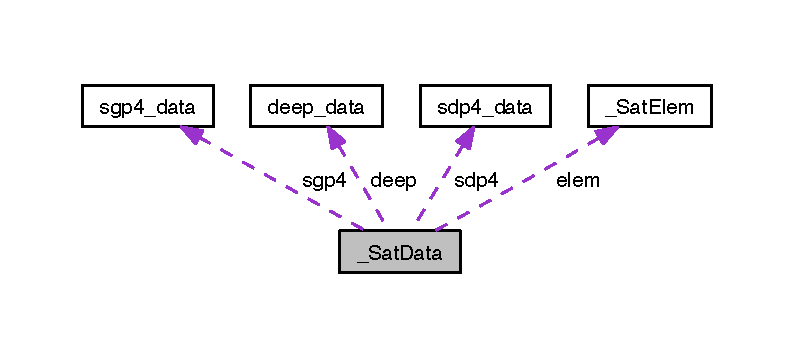
\includegraphics[width=350pt]{struct___sat_data__coll__graph}
\end{center}
\end{figure}
\subsection*{Data Fields}
\begin{DoxyCompactItemize}
\item 
struct \hyperlink{struct___sat_elem}{\-\_\-\-Sat\-Elem} $\ast$ \hyperlink{struct___sat_data_a8f6ca40e052cd0bac7ed283fa35147ef}{elem}
\item 
\begin{tabbing}
xx\=xx\=xx\=xx\=xx\=xx\=xx\=xx\=xx\=\kill
union \{\\
\>struct \hyperlink{structsgp4__data}{sgp4\_data} $\ast$ \hyperlink{struct___sat_data_a67d36020c0d25eb5a4684978b7fd3df6}{sgp4}\\
\>struct \hyperlink{structsdp4__data}{sdp4\_data} $\ast$ \hyperlink{struct___sat_data_ab7bfd91966db6411332426656d1a62f4}{sdp4}\\
\} \hyperlink{struct___sat_data_afdd865c8d5f71af2985b7292db552364}{prop}\\

\end{tabbing}\item 
struct \hyperlink{structdeep__data}{deep\-\_\-data} $\ast$ \hyperlink{struct___sat_data_aaa92af6491d38cb39ac15847e645d907}{deep}
\end{DoxyCompactItemize}


\subsection{Detailed Description}


Definition at line 189 of file satlib.\-h.



\subsection{Field Documentation}
\hypertarget{struct___sat_data_aaa92af6491d38cb39ac15847e645d907}{\index{\-\_\-\-Sat\-Data@{\-\_\-\-Sat\-Data}!deep@{deep}}
\index{deep@{deep}!_SatData@{\-\_\-\-Sat\-Data}}
\subsubsection[{deep}]{\setlength{\rightskip}{0pt plus 5cm}struct {\bf deep\-\_\-data}$\ast$ \-\_\-\-Sat\-Data\-::deep}}\label{struct___sat_data_aaa92af6491d38cb39ac15847e645d907}


Definition at line 195 of file satlib.\-h.

\hypertarget{struct___sat_data_a8f6ca40e052cd0bac7ed283fa35147ef}{\index{\-\_\-\-Sat\-Data@{\-\_\-\-Sat\-Data}!elem@{elem}}
\index{elem@{elem}!_SatData@{\-\_\-\-Sat\-Data}}
\subsubsection[{elem}]{\setlength{\rightskip}{0pt plus 5cm}struct {\bf \-\_\-\-Sat\-Elem}$\ast$ \-\_\-\-Sat\-Data\-::elem}}\label{struct___sat_data_a8f6ca40e052cd0bac7ed283fa35147ef}


Definition at line 190 of file satlib.\-h.

\hypertarget{struct___sat_data_afdd865c8d5f71af2985b7292db552364}{\index{\-\_\-\-Sat\-Data@{\-\_\-\-Sat\-Data}!prop@{prop}}
\index{prop@{prop}!_SatData@{\-\_\-\-Sat\-Data}}
\subsubsection[{prop}]{\setlength{\rightskip}{0pt plus 5cm}union \{ ... \}   \-\_\-\-Sat\-Data\-::prop}}\label{struct___sat_data_afdd865c8d5f71af2985b7292db552364}
\hypertarget{struct___sat_data_ab7bfd91966db6411332426656d1a62f4}{\index{\-\_\-\-Sat\-Data@{\-\_\-\-Sat\-Data}!sdp4@{sdp4}}
\index{sdp4@{sdp4}!_SatData@{\-\_\-\-Sat\-Data}}
\subsubsection[{sdp4}]{\setlength{\rightskip}{0pt plus 5cm}struct {\bf sdp4\-\_\-data}$\ast$ \-\_\-\-Sat\-Data\-::sdp4}}\label{struct___sat_data_ab7bfd91966db6411332426656d1a62f4}


Definition at line 193 of file satlib.\-h.

\hypertarget{struct___sat_data_a67d36020c0d25eb5a4684978b7fd3df6}{\index{\-\_\-\-Sat\-Data@{\-\_\-\-Sat\-Data}!sgp4@{sgp4}}
\index{sgp4@{sgp4}!_SatData@{\-\_\-\-Sat\-Data}}
\subsubsection[{sgp4}]{\setlength{\rightskip}{0pt plus 5cm}struct {\bf sgp4\-\_\-data}$\ast$ \-\_\-\-Sat\-Data\-::sgp4}}\label{struct___sat_data_a67d36020c0d25eb5a4684978b7fd3df6}


Definition at line 192 of file satlib.\-h.



The documentation for this struct was generated from the following file\-:\begin{DoxyCompactItemize}
\item 
libastro/\hyperlink{satlib_8h}{satlib.\-h}\end{DoxyCompactItemize}

\hypertarget{struct___sat_elem}{\section{\-\_\-\-Sat\-Elem Struct Reference}
\label{struct___sat_elem}\index{\-\_\-\-Sat\-Elem@{\-\_\-\-Sat\-Elem}}
}


{\ttfamily \#include $<$satlib.\-h$>$}

\subsection*{Data Fields}
\begin{DoxyCompactItemize}
\item 
float \hyperlink{struct___sat_elem_aa146285d54323061c76de2405e64c6bf}{se\-\_\-\-X\-M\-O}
\item 
float \hyperlink{struct___sat_elem_a74d35f2c9772d5951cb24aa631e3e4df}{se\-\_\-\-X\-N\-O\-D\-E\-O}
\item 
float \hyperlink{struct___sat_elem_af530e5942e833b59ba385cacbed189e0}{se\-\_\-\-O\-M\-E\-G\-A\-O}
\item 
float \hyperlink{struct___sat_elem_a11986bb255a52da8614cfacc1155bf89}{se\-\_\-\-E\-O}
\item 
float \hyperlink{struct___sat_elem_a5a9a336e24ea5df7051e5ce3b126a87e}{se\-\_\-\-X\-I\-N\-C\-L}
\item 
float \hyperlink{struct___sat_elem_aae09d71117e666583cbcf89186b10865}{se\-\_\-\-X\-N\-D\-D60}
\item 
float \hyperlink{struct___sat_elem_a282db948ea254d1ca2de2dfc9ee698c0}{se\-\_\-\-B\-S\-T\-A\-R}
\item 
float \hyperlink{struct___sat_elem_afdbc8e77fc81473ca1baa8f1f9b68f25}{pad1}
\item 
double \hyperlink{struct___sat_elem_aafa866947f4ac775274333db067aac77}{se\-\_\-\-X\-N\-O}
\item 
double \hyperlink{struct___sat_elem_a7dbd7b9b28a50bfbe0313592200f02b3}{se\-\_\-\-X\-N\-D\-T20}
\item 
double \hyperlink{struct___sat_elem_a31e22c4bf1c6745eaa88c19e1fb78cab}{se\-\_\-\-E\-P\-O\-C\-H}
\item 
\begin{tabbing}
xx\=xx\=xx\=xx\=xx\=xx\=xx\=xx\=xx\=\kill
struct \{\\
\>unsigned int \hyperlink{struct___sat_elem_a1bf11c0e76b4a6e2e34485990276cca6}{catno}: 21\\
\>unsigned int \hyperlink{struct___sat_elem_a99c4f0b298134a76356c70ae6cf13a26}{classif}: 5\\
\>unsigned int \hyperlink{struct___sat_elem_a8f27690ed10a4c11f8347d15cc339f03}{elnum}: 10\\
\>unsigned int \hyperlink{struct___sat_elem_a203379207f7fc2daca8632f639950974}{year}: 14\\
\>unsigned int \hyperlink{struct___sat_elem_a78bf01cbb8fcb2cbd6b896b6ca88ff0c}{launch}: 10\\
\>unsigned int \hyperlink{struct___sat_elem_a94bd5ae73f4c4bb55677d3a0e998eef2}{piece}: 15\\
\>unsigned int \hyperlink{struct___sat_elem_a84743e8c5b4eed8213b2402e1d5ef7f4}{ephtype}: 4\\
\>unsigned int \hyperlink{struct___sat_elem_a44123ee50a25e6ec959b8683803e561e}{orbit}: 17\\
\} \hyperlink{struct___sat_elem_af713f30c8d04002d6b3f7ac53c19740e}{se\_id}\\

\end{tabbing}\end{DoxyCompactItemize}


\subsection{Detailed Description}


Definition at line 6 of file satlib.\-h.



\subsection{Field Documentation}
\hypertarget{struct___sat_elem_a1bf11c0e76b4a6e2e34485990276cca6}{\index{\-\_\-\-Sat\-Elem@{\-\_\-\-Sat\-Elem}!catno@{catno}}
\index{catno@{catno}!_SatElem@{\-\_\-\-Sat\-Elem}}
\subsubsection[{catno}]{\setlength{\rightskip}{0pt plus 5cm}unsigned int \-\_\-\-Sat\-Elem\-::catno}}\label{struct___sat_elem_a1bf11c0e76b4a6e2e34485990276cca6}


Definition at line 19 of file satlib.\-h.

\hypertarget{struct___sat_elem_a99c4f0b298134a76356c70ae6cf13a26}{\index{\-\_\-\-Sat\-Elem@{\-\_\-\-Sat\-Elem}!classif@{classif}}
\index{classif@{classif}!_SatElem@{\-\_\-\-Sat\-Elem}}
\subsubsection[{classif}]{\setlength{\rightskip}{0pt plus 5cm}unsigned int \-\_\-\-Sat\-Elem\-::classif}}\label{struct___sat_elem_a99c4f0b298134a76356c70ae6cf13a26}


Definition at line 20 of file satlib.\-h.

\hypertarget{struct___sat_elem_a8f27690ed10a4c11f8347d15cc339f03}{\index{\-\_\-\-Sat\-Elem@{\-\_\-\-Sat\-Elem}!elnum@{elnum}}
\index{elnum@{elnum}!_SatElem@{\-\_\-\-Sat\-Elem}}
\subsubsection[{elnum}]{\setlength{\rightskip}{0pt plus 5cm}unsigned int \-\_\-\-Sat\-Elem\-::elnum}}\label{struct___sat_elem_a8f27690ed10a4c11f8347d15cc339f03}


Definition at line 21 of file satlib.\-h.

\hypertarget{struct___sat_elem_a84743e8c5b4eed8213b2402e1d5ef7f4}{\index{\-\_\-\-Sat\-Elem@{\-\_\-\-Sat\-Elem}!ephtype@{ephtype}}
\index{ephtype@{ephtype}!_SatElem@{\-\_\-\-Sat\-Elem}}
\subsubsection[{ephtype}]{\setlength{\rightskip}{0pt plus 5cm}unsigned int \-\_\-\-Sat\-Elem\-::ephtype}}\label{struct___sat_elem_a84743e8c5b4eed8213b2402e1d5ef7f4}


Definition at line 25 of file satlib.\-h.

\hypertarget{struct___sat_elem_a78bf01cbb8fcb2cbd6b896b6ca88ff0c}{\index{\-\_\-\-Sat\-Elem@{\-\_\-\-Sat\-Elem}!launch@{launch}}
\index{launch@{launch}!_SatElem@{\-\_\-\-Sat\-Elem}}
\subsubsection[{launch}]{\setlength{\rightskip}{0pt plus 5cm}unsigned int \-\_\-\-Sat\-Elem\-::launch}}\label{struct___sat_elem_a78bf01cbb8fcb2cbd6b896b6ca88ff0c}


Definition at line 23 of file satlib.\-h.

\hypertarget{struct___sat_elem_a44123ee50a25e6ec959b8683803e561e}{\index{\-\_\-\-Sat\-Elem@{\-\_\-\-Sat\-Elem}!orbit@{orbit}}
\index{orbit@{orbit}!_SatElem@{\-\_\-\-Sat\-Elem}}
\subsubsection[{orbit}]{\setlength{\rightskip}{0pt plus 5cm}unsigned int \-\_\-\-Sat\-Elem\-::orbit}}\label{struct___sat_elem_a44123ee50a25e6ec959b8683803e561e}


Definition at line 26 of file satlib.\-h.

\hypertarget{struct___sat_elem_afdbc8e77fc81473ca1baa8f1f9b68f25}{\index{\-\_\-\-Sat\-Elem@{\-\_\-\-Sat\-Elem}!pad1@{pad1}}
\index{pad1@{pad1}!_SatElem@{\-\_\-\-Sat\-Elem}}
\subsubsection[{pad1}]{\setlength{\rightskip}{0pt plus 5cm}float \-\_\-\-Sat\-Elem\-::pad1}}\label{struct___sat_elem_afdbc8e77fc81473ca1baa8f1f9b68f25}


Definition at line 14 of file satlib.\-h.

\hypertarget{struct___sat_elem_a94bd5ae73f4c4bb55677d3a0e998eef2}{\index{\-\_\-\-Sat\-Elem@{\-\_\-\-Sat\-Elem}!piece@{piece}}
\index{piece@{piece}!_SatElem@{\-\_\-\-Sat\-Elem}}
\subsubsection[{piece}]{\setlength{\rightskip}{0pt plus 5cm}unsigned int \-\_\-\-Sat\-Elem\-::piece}}\label{struct___sat_elem_a94bd5ae73f4c4bb55677d3a0e998eef2}


Definition at line 24 of file satlib.\-h.

\hypertarget{struct___sat_elem_a282db948ea254d1ca2de2dfc9ee698c0}{\index{\-\_\-\-Sat\-Elem@{\-\_\-\-Sat\-Elem}!se\-\_\-\-B\-S\-T\-A\-R@{se\-\_\-\-B\-S\-T\-A\-R}}
\index{se\-\_\-\-B\-S\-T\-A\-R@{se\-\_\-\-B\-S\-T\-A\-R}!_SatElem@{\-\_\-\-Sat\-Elem}}
\subsubsection[{se\-\_\-\-B\-S\-T\-A\-R}]{\setlength{\rightskip}{0pt plus 5cm}float \-\_\-\-Sat\-Elem\-::se\-\_\-\-B\-S\-T\-A\-R}}\label{struct___sat_elem_a282db948ea254d1ca2de2dfc9ee698c0}


Definition at line 13 of file satlib.\-h.

\hypertarget{struct___sat_elem_a11986bb255a52da8614cfacc1155bf89}{\index{\-\_\-\-Sat\-Elem@{\-\_\-\-Sat\-Elem}!se\-\_\-\-E\-O@{se\-\_\-\-E\-O}}
\index{se\-\_\-\-E\-O@{se\-\_\-\-E\-O}!_SatElem@{\-\_\-\-Sat\-Elem}}
\subsubsection[{se\-\_\-\-E\-O}]{\setlength{\rightskip}{0pt plus 5cm}float \-\_\-\-Sat\-Elem\-::se\-\_\-\-E\-O}}\label{struct___sat_elem_a11986bb255a52da8614cfacc1155bf89}


Definition at line 10 of file satlib.\-h.

\hypertarget{struct___sat_elem_a31e22c4bf1c6745eaa88c19e1fb78cab}{\index{\-\_\-\-Sat\-Elem@{\-\_\-\-Sat\-Elem}!se\-\_\-\-E\-P\-O\-C\-H@{se\-\_\-\-E\-P\-O\-C\-H}}
\index{se\-\_\-\-E\-P\-O\-C\-H@{se\-\_\-\-E\-P\-O\-C\-H}!_SatElem@{\-\_\-\-Sat\-Elem}}
\subsubsection[{se\-\_\-\-E\-P\-O\-C\-H}]{\setlength{\rightskip}{0pt plus 5cm}double \-\_\-\-Sat\-Elem\-::se\-\_\-\-E\-P\-O\-C\-H}}\label{struct___sat_elem_a31e22c4bf1c6745eaa88c19e1fb78cab}


Definition at line 17 of file satlib.\-h.

\hypertarget{struct___sat_elem_af713f30c8d04002d6b3f7ac53c19740e}{\index{\-\_\-\-Sat\-Elem@{\-\_\-\-Sat\-Elem}!se\-\_\-id@{se\-\_\-id}}
\index{se\-\_\-id@{se\-\_\-id}!_SatElem@{\-\_\-\-Sat\-Elem}}
\subsubsection[{se\-\_\-id}]{\setlength{\rightskip}{0pt plus 5cm}struct \{ ... \}   \-\_\-\-Sat\-Elem\-::se\-\_\-id}}\label{struct___sat_elem_af713f30c8d04002d6b3f7ac53c19740e}
\hypertarget{struct___sat_elem_af530e5942e833b59ba385cacbed189e0}{\index{\-\_\-\-Sat\-Elem@{\-\_\-\-Sat\-Elem}!se\-\_\-\-O\-M\-E\-G\-A\-O@{se\-\_\-\-O\-M\-E\-G\-A\-O}}
\index{se\-\_\-\-O\-M\-E\-G\-A\-O@{se\-\_\-\-O\-M\-E\-G\-A\-O}!_SatElem@{\-\_\-\-Sat\-Elem}}
\subsubsection[{se\-\_\-\-O\-M\-E\-G\-A\-O}]{\setlength{\rightskip}{0pt plus 5cm}float \-\_\-\-Sat\-Elem\-::se\-\_\-\-O\-M\-E\-G\-A\-O}}\label{struct___sat_elem_af530e5942e833b59ba385cacbed189e0}


Definition at line 9 of file satlib.\-h.

\hypertarget{struct___sat_elem_a5a9a336e24ea5df7051e5ce3b126a87e}{\index{\-\_\-\-Sat\-Elem@{\-\_\-\-Sat\-Elem}!se\-\_\-\-X\-I\-N\-C\-L@{se\-\_\-\-X\-I\-N\-C\-L}}
\index{se\-\_\-\-X\-I\-N\-C\-L@{se\-\_\-\-X\-I\-N\-C\-L}!_SatElem@{\-\_\-\-Sat\-Elem}}
\subsubsection[{se\-\_\-\-X\-I\-N\-C\-L}]{\setlength{\rightskip}{0pt plus 5cm}float \-\_\-\-Sat\-Elem\-::se\-\_\-\-X\-I\-N\-C\-L}}\label{struct___sat_elem_a5a9a336e24ea5df7051e5ce3b126a87e}


Definition at line 11 of file satlib.\-h.

\hypertarget{struct___sat_elem_aa146285d54323061c76de2405e64c6bf}{\index{\-\_\-\-Sat\-Elem@{\-\_\-\-Sat\-Elem}!se\-\_\-\-X\-M\-O@{se\-\_\-\-X\-M\-O}}
\index{se\-\_\-\-X\-M\-O@{se\-\_\-\-X\-M\-O}!_SatElem@{\-\_\-\-Sat\-Elem}}
\subsubsection[{se\-\_\-\-X\-M\-O}]{\setlength{\rightskip}{0pt plus 5cm}float \-\_\-\-Sat\-Elem\-::se\-\_\-\-X\-M\-O}}\label{struct___sat_elem_aa146285d54323061c76de2405e64c6bf}


Definition at line 7 of file satlib.\-h.

\hypertarget{struct___sat_elem_aae09d71117e666583cbcf89186b10865}{\index{\-\_\-\-Sat\-Elem@{\-\_\-\-Sat\-Elem}!se\-\_\-\-X\-N\-D\-D60@{se\-\_\-\-X\-N\-D\-D60}}
\index{se\-\_\-\-X\-N\-D\-D60@{se\-\_\-\-X\-N\-D\-D60}!_SatElem@{\-\_\-\-Sat\-Elem}}
\subsubsection[{se\-\_\-\-X\-N\-D\-D60}]{\setlength{\rightskip}{0pt plus 5cm}float \-\_\-\-Sat\-Elem\-::se\-\_\-\-X\-N\-D\-D60}}\label{struct___sat_elem_aae09d71117e666583cbcf89186b10865}


Definition at line 12 of file satlib.\-h.

\hypertarget{struct___sat_elem_a7dbd7b9b28a50bfbe0313592200f02b3}{\index{\-\_\-\-Sat\-Elem@{\-\_\-\-Sat\-Elem}!se\-\_\-\-X\-N\-D\-T20@{se\-\_\-\-X\-N\-D\-T20}}
\index{se\-\_\-\-X\-N\-D\-T20@{se\-\_\-\-X\-N\-D\-T20}!_SatElem@{\-\_\-\-Sat\-Elem}}
\subsubsection[{se\-\_\-\-X\-N\-D\-T20}]{\setlength{\rightskip}{0pt plus 5cm}double \-\_\-\-Sat\-Elem\-::se\-\_\-\-X\-N\-D\-T20}}\label{struct___sat_elem_a7dbd7b9b28a50bfbe0313592200f02b3}


Definition at line 16 of file satlib.\-h.

\hypertarget{struct___sat_elem_aafa866947f4ac775274333db067aac77}{\index{\-\_\-\-Sat\-Elem@{\-\_\-\-Sat\-Elem}!se\-\_\-\-X\-N\-O@{se\-\_\-\-X\-N\-O}}
\index{se\-\_\-\-X\-N\-O@{se\-\_\-\-X\-N\-O}!_SatElem@{\-\_\-\-Sat\-Elem}}
\subsubsection[{se\-\_\-\-X\-N\-O}]{\setlength{\rightskip}{0pt plus 5cm}double \-\_\-\-Sat\-Elem\-::se\-\_\-\-X\-N\-O}}\label{struct___sat_elem_aafa866947f4ac775274333db067aac77}


Definition at line 15 of file satlib.\-h.

\hypertarget{struct___sat_elem_a74d35f2c9772d5951cb24aa631e3e4df}{\index{\-\_\-\-Sat\-Elem@{\-\_\-\-Sat\-Elem}!se\-\_\-\-X\-N\-O\-D\-E\-O@{se\-\_\-\-X\-N\-O\-D\-E\-O}}
\index{se\-\_\-\-X\-N\-O\-D\-E\-O@{se\-\_\-\-X\-N\-O\-D\-E\-O}!_SatElem@{\-\_\-\-Sat\-Elem}}
\subsubsection[{se\-\_\-\-X\-N\-O\-D\-E\-O}]{\setlength{\rightskip}{0pt plus 5cm}float \-\_\-\-Sat\-Elem\-::se\-\_\-\-X\-N\-O\-D\-E\-O}}\label{struct___sat_elem_a74d35f2c9772d5951cb24aa631e3e4df}


Definition at line 8 of file satlib.\-h.

\hypertarget{struct___sat_elem_a203379207f7fc2daca8632f639950974}{\index{\-\_\-\-Sat\-Elem@{\-\_\-\-Sat\-Elem}!year@{year}}
\index{year@{year}!_SatElem@{\-\_\-\-Sat\-Elem}}
\subsubsection[{year}]{\setlength{\rightskip}{0pt plus 5cm}unsigned int \-\_\-\-Sat\-Elem\-::year}}\label{struct___sat_elem_a203379207f7fc2daca8632f639950974}


Definition at line 22 of file satlib.\-h.



The documentation for this struct was generated from the following file\-:\begin{DoxyCompactItemize}
\item 
libastro/\hyperlink{satlib_8h}{satlib.\-h}\end{DoxyCompactItemize}

\hypertarget{struct___vec3}{\section{\-\_\-\-Vec3 Struct Reference}
\label{struct___vec3}\index{\-\_\-\-Vec3@{\-\_\-\-Vec3}}
}


{\ttfamily \#include $<$sattypes.\-h$>$}

\subsection*{Data Fields}
\begin{DoxyCompactItemize}
\item 
double \hyperlink{struct___vec3_a89f05408b1ce51aa836cbf99bd79aaaa}{x}
\item 
double \hyperlink{struct___vec3_aadf0c086ad7cccecb4c84b540d60d490}{y}
\item 
double \hyperlink{struct___vec3_a00c51a769832f289d58ad4ec07331ab8}{z}
\end{DoxyCompactItemize}


\subsection{Detailed Description}


Definition at line 6 of file sattypes.\-h.



\subsection{Field Documentation}
\hypertarget{struct___vec3_a89f05408b1ce51aa836cbf99bd79aaaa}{\index{\-\_\-\-Vec3@{\-\_\-\-Vec3}!x@{x}}
\index{x@{x}!_Vec3@{\-\_\-\-Vec3}}
\subsubsection[{x}]{\setlength{\rightskip}{0pt plus 5cm}double \-\_\-\-Vec3\-::x}}\label{struct___vec3_a89f05408b1ce51aa836cbf99bd79aaaa}


Definition at line 7 of file sattypes.\-h.

\hypertarget{struct___vec3_aadf0c086ad7cccecb4c84b540d60d490}{\index{\-\_\-\-Vec3@{\-\_\-\-Vec3}!y@{y}}
\index{y@{y}!_Vec3@{\-\_\-\-Vec3}}
\subsubsection[{y}]{\setlength{\rightskip}{0pt plus 5cm}double \-\_\-\-Vec3\-::y}}\label{struct___vec3_aadf0c086ad7cccecb4c84b540d60d490}


Definition at line 7 of file sattypes.\-h.

\hypertarget{struct___vec3_a00c51a769832f289d58ad4ec07331ab8}{\index{\-\_\-\-Vec3@{\-\_\-\-Vec3}!z@{z}}
\index{z@{z}!_Vec3@{\-\_\-\-Vec3}}
\subsubsection[{z}]{\setlength{\rightskip}{0pt plus 5cm}double \-\_\-\-Vec3\-::z}}\label{struct___vec3_a00c51a769832f289d58ad4ec07331ab8}


Definition at line 7 of file sattypes.\-h.



The documentation for this struct was generated from the following file\-:\begin{DoxyCompactItemize}
\item 
libastro/\hyperlink{sattypes_8h}{sattypes.\-h}\end{DoxyCompactItemize}

\hypertarget{struct_bin_orbit}{\section{Bin\-Orbit Struct Reference}
\label{struct_bin_orbit}\index{Bin\-Orbit@{Bin\-Orbit}}
}


{\ttfamily \#include $<$astro.\-h$>$}

\subsection*{Data Fields}
\begin{DoxyCompactItemize}
\item 
float \hyperlink{struct_bin_orbit_a13a14fdb480f7e64a11a574f6c3a4c74}{bo\-\_\-\-T}
\item 
float \hyperlink{struct_bin_orbit_a153e76ae7fbba6c5d51db5c849712fd7}{bo\-\_\-e}
\item 
float \hyperlink{struct_bin_orbit_a7ed2ce32869bece7d6f19ad4513c8ca1}{bo\-\_\-o}
\item 
float \hyperlink{struct_bin_orbit_a4b329066d26ceae03acbcaf73b2eee9c}{bo\-\_\-\-O}
\item 
float \hyperlink{struct_bin_orbit_ac352c440ca03b4fb61318b7af937a272}{bo\-\_\-i}
\item 
float \hyperlink{struct_bin_orbit_a678bd2f8ce272811bbda8eb371bc9199}{bo\-\_\-a}
\item 
float \hyperlink{struct_bin_orbit_ada0bcef01f07cd152cf994e004276b25}{bo\-\_\-\-P}
\item 
float \hyperlink{struct_bin_orbit_ad3fedf474fce6b3a979767b6e87bcf89}{bo\-\_\-pa}
\item 
float \hyperlink{struct_bin_orbit_afbdda06daa8e30a7737c039351262e99}{bo\-\_\-sep}
\item 
float \hyperlink{struct_bin_orbit_a1d4a15be4410fce37882ba20ba589af0}{bo\-\_\-ra}
\item 
float \hyperlink{struct_bin_orbit_adbdb17536ddf22681e9d3ec9aa140ee2}{bo\-\_\-dec}
\end{DoxyCompactItemize}


\subsection{Detailed Description}


Definition at line 189 of file astro.\-h.



\subsection{Field Documentation}
\hypertarget{struct_bin_orbit_a678bd2f8ce272811bbda8eb371bc9199}{\index{Bin\-Orbit@{Bin\-Orbit}!bo\-\_\-a@{bo\-\_\-a}}
\index{bo\-\_\-a@{bo\-\_\-a}!BinOrbit@{Bin\-Orbit}}
\subsubsection[{bo\-\_\-a}]{\setlength{\rightskip}{0pt plus 5cm}float Bin\-Orbit\-::bo\-\_\-a}}\label{struct_bin_orbit_a678bd2f8ce272811bbda8eb371bc9199}


Definition at line 195 of file astro.\-h.

\hypertarget{struct_bin_orbit_adbdb17536ddf22681e9d3ec9aa140ee2}{\index{Bin\-Orbit@{Bin\-Orbit}!bo\-\_\-dec@{bo\-\_\-dec}}
\index{bo\-\_\-dec@{bo\-\_\-dec}!BinOrbit@{Bin\-Orbit}}
\subsubsection[{bo\-\_\-dec}]{\setlength{\rightskip}{0pt plus 5cm}float Bin\-Orbit\-::bo\-\_\-dec}}\label{struct_bin_orbit_adbdb17536ddf22681e9d3ec9aa140ee2}


Definition at line 202 of file astro.\-h.

\hypertarget{struct_bin_orbit_a153e76ae7fbba6c5d51db5c849712fd7}{\index{Bin\-Orbit@{Bin\-Orbit}!bo\-\_\-e@{bo\-\_\-e}}
\index{bo\-\_\-e@{bo\-\_\-e}!BinOrbit@{Bin\-Orbit}}
\subsubsection[{bo\-\_\-e}]{\setlength{\rightskip}{0pt plus 5cm}float Bin\-Orbit\-::bo\-\_\-e}}\label{struct_bin_orbit_a153e76ae7fbba6c5d51db5c849712fd7}


Definition at line 191 of file astro.\-h.

\hypertarget{struct_bin_orbit_ac352c440ca03b4fb61318b7af937a272}{\index{Bin\-Orbit@{Bin\-Orbit}!bo\-\_\-i@{bo\-\_\-i}}
\index{bo\-\_\-i@{bo\-\_\-i}!BinOrbit@{Bin\-Orbit}}
\subsubsection[{bo\-\_\-i}]{\setlength{\rightskip}{0pt plus 5cm}float Bin\-Orbit\-::bo\-\_\-i}}\label{struct_bin_orbit_ac352c440ca03b4fb61318b7af937a272}


Definition at line 194 of file astro.\-h.

\hypertarget{struct_bin_orbit_a7ed2ce32869bece7d6f19ad4513c8ca1}{\index{Bin\-Orbit@{Bin\-Orbit}!bo\-\_\-o@{bo\-\_\-o}}
\index{bo\-\_\-o@{bo\-\_\-o}!BinOrbit@{Bin\-Orbit}}
\subsubsection[{bo\-\_\-o}]{\setlength{\rightskip}{0pt plus 5cm}float Bin\-Orbit\-::bo\-\_\-o}}\label{struct_bin_orbit_a7ed2ce32869bece7d6f19ad4513c8ca1}


Definition at line 192 of file astro.\-h.

\hypertarget{struct_bin_orbit_a4b329066d26ceae03acbcaf73b2eee9c}{\index{Bin\-Orbit@{Bin\-Orbit}!bo\-\_\-\-O@{bo\-\_\-\-O}}
\index{bo\-\_\-\-O@{bo\-\_\-\-O}!BinOrbit@{Bin\-Orbit}}
\subsubsection[{bo\-\_\-\-O}]{\setlength{\rightskip}{0pt plus 5cm}float Bin\-Orbit\-::bo\-\_\-\-O}}\label{struct_bin_orbit_a4b329066d26ceae03acbcaf73b2eee9c}


Definition at line 193 of file astro.\-h.

\hypertarget{struct_bin_orbit_ada0bcef01f07cd152cf994e004276b25}{\index{Bin\-Orbit@{Bin\-Orbit}!bo\-\_\-\-P@{bo\-\_\-\-P}}
\index{bo\-\_\-\-P@{bo\-\_\-\-P}!BinOrbit@{Bin\-Orbit}}
\subsubsection[{bo\-\_\-\-P}]{\setlength{\rightskip}{0pt plus 5cm}float Bin\-Orbit\-::bo\-\_\-\-P}}\label{struct_bin_orbit_ada0bcef01f07cd152cf994e004276b25}


Definition at line 196 of file astro.\-h.

\hypertarget{struct_bin_orbit_ad3fedf474fce6b3a979767b6e87bcf89}{\index{Bin\-Orbit@{Bin\-Orbit}!bo\-\_\-pa@{bo\-\_\-pa}}
\index{bo\-\_\-pa@{bo\-\_\-pa}!BinOrbit@{Bin\-Orbit}}
\subsubsection[{bo\-\_\-pa}]{\setlength{\rightskip}{0pt plus 5cm}float Bin\-Orbit\-::bo\-\_\-pa}}\label{struct_bin_orbit_ad3fedf474fce6b3a979767b6e87bcf89}


Definition at line 199 of file astro.\-h.

\hypertarget{struct_bin_orbit_a1d4a15be4410fce37882ba20ba589af0}{\index{Bin\-Orbit@{Bin\-Orbit}!bo\-\_\-ra@{bo\-\_\-ra}}
\index{bo\-\_\-ra@{bo\-\_\-ra}!BinOrbit@{Bin\-Orbit}}
\subsubsection[{bo\-\_\-ra}]{\setlength{\rightskip}{0pt plus 5cm}float Bin\-Orbit\-::bo\-\_\-ra}}\label{struct_bin_orbit_a1d4a15be4410fce37882ba20ba589af0}


Definition at line 201 of file astro.\-h.

\hypertarget{struct_bin_orbit_afbdda06daa8e30a7737c039351262e99}{\index{Bin\-Orbit@{Bin\-Orbit}!bo\-\_\-sep@{bo\-\_\-sep}}
\index{bo\-\_\-sep@{bo\-\_\-sep}!BinOrbit@{Bin\-Orbit}}
\subsubsection[{bo\-\_\-sep}]{\setlength{\rightskip}{0pt plus 5cm}float Bin\-Orbit\-::bo\-\_\-sep}}\label{struct_bin_orbit_afbdda06daa8e30a7737c039351262e99}


Definition at line 200 of file astro.\-h.

\hypertarget{struct_bin_orbit_a13a14fdb480f7e64a11a574f6c3a4c74}{\index{Bin\-Orbit@{Bin\-Orbit}!bo\-\_\-\-T@{bo\-\_\-\-T}}
\index{bo\-\_\-\-T@{bo\-\_\-\-T}!BinOrbit@{Bin\-Orbit}}
\subsubsection[{bo\-\_\-\-T}]{\setlength{\rightskip}{0pt plus 5cm}float Bin\-Orbit\-::bo\-\_\-\-T}}\label{struct_bin_orbit_a13a14fdb480f7e64a11a574f6c3a4c74}


Definition at line 190 of file astro.\-h.



The documentation for this struct was generated from the following file\-:\begin{DoxyCompactItemize}
\item 
libastro/\hyperlink{astro_8h}{astro.\-h}\end{DoxyCompactItemize}

\hypertarget{struct_bin_pos}{\section{Bin\-Pos Struct Reference}
\label{struct_bin_pos}\index{Bin\-Pos@{Bin\-Pos}}
}


{\ttfamily \#include $<$astro.\-h$>$}

\subsection*{Data Fields}
\begin{DoxyCompactItemize}
\item 
float \hyperlink{struct_bin_pos_ac1be5dd479308de781c96b87e299d1a5}{bp\-\_\-ep}
\item 
float \hyperlink{struct_bin_pos_a5a2e7d4cb399601758b0c724ce5543d4}{bp\-\_\-pa}
\item 
float \hyperlink{struct_bin_pos_aa451101e51c051196ee5cc0f6d846f77}{bp\-\_\-sep}
\item 
float \hyperlink{struct_bin_pos_addd6fc5c935d61f90723a4848e70c86f}{bp\-\_\-ra}
\item 
float \hyperlink{struct_bin_pos_a39f7d71c18cff409e741dffc6fce94e4}{bp\-\_\-dec}
\end{DoxyCompactItemize}


\subsection{Detailed Description}


Definition at line 204 of file astro.\-h.



\subsection{Field Documentation}
\hypertarget{struct_bin_pos_a39f7d71c18cff409e741dffc6fce94e4}{\index{Bin\-Pos@{Bin\-Pos}!bp\-\_\-dec@{bp\-\_\-dec}}
\index{bp\-\_\-dec@{bp\-\_\-dec}!BinPos@{Bin\-Pos}}
\subsubsection[{bp\-\_\-dec}]{\setlength{\rightskip}{0pt plus 5cm}float Bin\-Pos\-::bp\-\_\-dec}}\label{struct_bin_pos_a39f7d71c18cff409e741dffc6fce94e4}


Definition at line 211 of file astro.\-h.

\hypertarget{struct_bin_pos_ac1be5dd479308de781c96b87e299d1a5}{\index{Bin\-Pos@{Bin\-Pos}!bp\-\_\-ep@{bp\-\_\-ep}}
\index{bp\-\_\-ep@{bp\-\_\-ep}!BinPos@{Bin\-Pos}}
\subsubsection[{bp\-\_\-ep}]{\setlength{\rightskip}{0pt plus 5cm}float Bin\-Pos\-::bp\-\_\-ep}}\label{struct_bin_pos_ac1be5dd479308de781c96b87e299d1a5}


Definition at line 205 of file astro.\-h.

\hypertarget{struct_bin_pos_a5a2e7d4cb399601758b0c724ce5543d4}{\index{Bin\-Pos@{Bin\-Pos}!bp\-\_\-pa@{bp\-\_\-pa}}
\index{bp\-\_\-pa@{bp\-\_\-pa}!BinPos@{Bin\-Pos}}
\subsubsection[{bp\-\_\-pa}]{\setlength{\rightskip}{0pt plus 5cm}float Bin\-Pos\-::bp\-\_\-pa}}\label{struct_bin_pos_a5a2e7d4cb399601758b0c724ce5543d4}


Definition at line 206 of file astro.\-h.

\hypertarget{struct_bin_pos_addd6fc5c935d61f90723a4848e70c86f}{\index{Bin\-Pos@{Bin\-Pos}!bp\-\_\-ra@{bp\-\_\-ra}}
\index{bp\-\_\-ra@{bp\-\_\-ra}!BinPos@{Bin\-Pos}}
\subsubsection[{bp\-\_\-ra}]{\setlength{\rightskip}{0pt plus 5cm}float Bin\-Pos\-::bp\-\_\-ra}}\label{struct_bin_pos_addd6fc5c935d61f90723a4848e70c86f}


Definition at line 210 of file astro.\-h.

\hypertarget{struct_bin_pos_aa451101e51c051196ee5cc0f6d846f77}{\index{Bin\-Pos@{Bin\-Pos}!bp\-\_\-sep@{bp\-\_\-sep}}
\index{bp\-\_\-sep@{bp\-\_\-sep}!BinPos@{Bin\-Pos}}
\subsubsection[{bp\-\_\-sep}]{\setlength{\rightskip}{0pt plus 5cm}float Bin\-Pos\-::bp\-\_\-sep}}\label{struct_bin_pos_aa451101e51c051196ee5cc0f6d846f77}


Definition at line 207 of file astro.\-h.



The documentation for this struct was generated from the following file\-:\begin{DoxyCompactItemize}
\item 
libastro/\hyperlink{astro_8h}{astro.\-h}\end{DoxyCompactItemize}

\hypertarget{structchap95__rec}{\section{chap95\-\_\-rec Struct Reference}
\label{structchap95__rec}\index{chap95\-\_\-rec@{chap95\-\_\-rec}}
}


{\ttfamily \#include $<$chap95.\-h$>$}

\subsection*{Data Fields}
\begin{DoxyCompactItemize}
\item 
short \hyperlink{structchap95__rec_aede2c143b0232546b6b72f5c1baea673}{n}
\item 
double \hyperlink{structchap95__rec_a6b9ff076ab6312d71d591cc708cec4df}{amp} \mbox{[}6\mbox{]}
\item 
double \hyperlink{structchap95__rec_aefec81036fd6d6df1517ead20178ddeb}{Nu}
\end{DoxyCompactItemize}


\subsection{Detailed Description}


Definition at line 50 of file chap95.\-h.



\subsection{Field Documentation}
\hypertarget{structchap95__rec_a6b9ff076ab6312d71d591cc708cec4df}{\index{chap95\-\_\-rec@{chap95\-\_\-rec}!amp@{amp}}
\index{amp@{amp}!chap95_rec@{chap95\-\_\-rec}}
\subsubsection[{amp}]{\setlength{\rightskip}{0pt plus 5cm}double chap95\-\_\-rec\-::amp\mbox{[}6\mbox{]}}}\label{structchap95__rec_a6b9ff076ab6312d71d591cc708cec4df}


Definition at line 52 of file chap95.\-h.

\hypertarget{structchap95__rec_aede2c143b0232546b6b72f5c1baea673}{\index{chap95\-\_\-rec@{chap95\-\_\-rec}!n@{n}}
\index{n@{n}!chap95_rec@{chap95\-\_\-rec}}
\subsubsection[{n}]{\setlength{\rightskip}{0pt plus 5cm}short chap95\-\_\-rec\-::n}}\label{structchap95__rec_aede2c143b0232546b6b72f5c1baea673}


Definition at line 51 of file chap95.\-h.

\hypertarget{structchap95__rec_aefec81036fd6d6df1517ead20178ddeb}{\index{chap95\-\_\-rec@{chap95\-\_\-rec}!Nu@{Nu}}
\index{Nu@{Nu}!chap95_rec@{chap95\-\_\-rec}}
\subsubsection[{Nu}]{\setlength{\rightskip}{0pt plus 5cm}double chap95\-\_\-rec\-::\-Nu}}\label{structchap95__rec_aefec81036fd6d6df1517ead20178ddeb}


Definition at line 54 of file chap95.\-h.



The documentation for this struct was generated from the following file\-:\begin{DoxyCompactItemize}
\item 
libastro/\hyperlink{chap95_8h}{chap95.\-h}\end{DoxyCompactItemize}

\hypertarget{struct_con_fig}{\section{Con\-Fig Struct Reference}
\label{struct_con_fig}\index{Con\-Fig@{Con\-Fig}}
}
\subsection*{Data Fields}
\begin{DoxyCompactItemize}
\item 
int \hyperlink{struct_con_fig_acdfcee925b73c274d6a567bfeb77a4bc}{drawcode}
\item 
float \hyperlink{struct_con_fig_a3f87e2c516969cd5f37dcdd271f7eac5}{ra}
\item 
float \hyperlink{struct_con_fig_abc829a867f9ac9922a92a81838e8827a}{dec}
\end{DoxyCompactItemize}


\subsection{Detailed Description}


Definition at line 1621 of file constel.\-c.



\subsection{Field Documentation}
\hypertarget{struct_con_fig_abc829a867f9ac9922a92a81838e8827a}{\index{Con\-Fig@{Con\-Fig}!dec@{dec}}
\index{dec@{dec}!ConFig@{Con\-Fig}}
\subsubsection[{dec}]{\setlength{\rightskip}{0pt plus 5cm}float Con\-Fig\-::dec}}\label{struct_con_fig_abc829a867f9ac9922a92a81838e8827a}


Definition at line 1624 of file constel.\-c.

\hypertarget{struct_con_fig_acdfcee925b73c274d6a567bfeb77a4bc}{\index{Con\-Fig@{Con\-Fig}!drawcode@{drawcode}}
\index{drawcode@{drawcode}!ConFig@{Con\-Fig}}
\subsubsection[{drawcode}]{\setlength{\rightskip}{0pt plus 5cm}int Con\-Fig\-::drawcode}}\label{struct_con_fig_acdfcee925b73c274d6a567bfeb77a4bc}


Definition at line 1622 of file constel.\-c.

\hypertarget{struct_con_fig_a3f87e2c516969cd5f37dcdd271f7eac5}{\index{Con\-Fig@{Con\-Fig}!ra@{ra}}
\index{ra@{ra}!ConFig@{Con\-Fig}}
\subsubsection[{ra}]{\setlength{\rightskip}{0pt plus 5cm}float Con\-Fig\-::ra}}\label{struct_con_fig_a3f87e2c516969cd5f37dcdd271f7eac5}


Definition at line 1623 of file constel.\-c.



The documentation for this struct was generated from the following file\-:\begin{DoxyCompactItemize}
\item 
libastro/\hyperlink{constel_8c}{constel.\-c}\end{DoxyCompactItemize}

\hypertarget{structdeep__data}{\section{deep\-\_\-data Struct Reference}
\label{structdeep__data}\index{deep\-\_\-data@{deep\-\_\-data}}
}


{\ttfamily \#include $<$satlib.\-h$>$}

\subsection*{Data Fields}
\begin{DoxyCompactItemize}
\item 
\begin{tabbing}
xx\=xx\=xx\=xx\=xx\=xx\=xx\=xx\=xx\=\kill
struct \{\\
\>unsigned int \hyperlink{structdeep__data_aa483e28efccb3251ed4ab9a8acc87cf1}{IRESFL}: 1\\
\>unsigned int \hyperlink{structdeep__data_a50c7c2c3f446f082e85caeebe42b6334}{ISYNFL}: 1\\
\} \hyperlink{structdeep__data_a000d674d79348a7f2df37166bc0c6852}{deep\_flags}\\

\end{tabbing}\item 
double \hyperlink{structdeep__data_a5479a146e76ceeeb6b39b8e2dc86423a}{deep\-\_\-s\-\_\-\-S\-I\-N\-I\-Q}
\item 
double \hyperlink{structdeep__data_aeb703feb0275a9df4c3f203f549cf68e}{deep\-\_\-s\-\_\-\-C\-O\-S\-I\-Q}
\item 
double \hyperlink{structdeep__data_a8f25fa88406d398af7e3dc77f5756492}{deep\-\_\-s\-\_\-\-O\-M\-G\-D\-T}
\item 
double \hyperlink{structdeep__data_a87e329466e9fc5dc95bca1bd0cbe036a}{deep\-\_\-\-A\-T\-I\-M\-E}
\item 
double \hyperlink{structdeep__data_ac16b78edb009129cc5ba63a684d7df06}{deep\-\_\-\-D2201}
\item 
double \hyperlink{structdeep__data_a0e6ac7d14886628f39b2dabbac5e9768}{deep\-\_\-\-D2211}
\item 
double \hyperlink{structdeep__data_a4d5d625f92b0af3ad25b4a12e4e13a7c}{deep\-\_\-\-D3210}
\item 
double \hyperlink{structdeep__data_ac121ab6ccd0b99df1566ff2348e75433}{deep\-\_\-\-D3222}
\item 
double \hyperlink{structdeep__data_a6777c25b08e398a519efa14ccc328b18}{deep\-\_\-\-D4410}
\item 
double \hyperlink{structdeep__data_a9ac99ac71a7e9d41e18e0b8d23881b27}{deep\-\_\-\-D4422}
\item 
double \hyperlink{structdeep__data_a070522e386b048a06c43a704492b63cd}{deep\-\_\-\-D5220}
\item 
double \hyperlink{structdeep__data_af6cb901bd696af94de75b2d78800db43}{deep\-\_\-\-D5232}
\item 
double \hyperlink{structdeep__data_a7f1d7113215d1faeeafcd818832f4da4}{deep\-\_\-\-D5421}
\item 
double \hyperlink{structdeep__data_ac7705b43b143e8a75b7a31f044000b19}{deep\-\_\-\-D5433}
\item 
double \hyperlink{structdeep__data_ae9e2a8ed7f2195320d1cd0fdb9b89dc4}{deep\-\_\-\-D\-E\-L1}
\item 
double \hyperlink{structdeep__data_aa6140563b789a280396850b260e6e33f}{deep\-\_\-\-D\-E\-L2}
\item 
double \hyperlink{structdeep__data_a1c596e0d8433da1dfb79124550ae55f3}{deep\-\_\-\-D\-E\-L3}
\item 
double \hyperlink{structdeep__data_a18bc60bed280f6304b0561e620a0fba1}{deep\-\_\-\-E3}
\item 
double \hyperlink{structdeep__data_ad56e8a78d8e4b1e77212692466325ea0}{deep\-\_\-\-E\-E2}
\item 
double \hyperlink{structdeep__data_a6860682a1c0a1bd96a6da624e58904f2}{deep\-\_\-\-F\-A\-S\-X2}
\item 
double \hyperlink{structdeep__data_a8da5269a610ed64efdb20ec003cedfff}{deep\-\_\-\-F\-A\-S\-X4}
\item 
double \hyperlink{structdeep__data_a7a83916118009f55fd5a3110f27cfc92}{deep\-\_\-\-F\-A\-S\-X6}
\item 
double \hyperlink{structdeep__data_a781f41e5be1a7461d09595a9f40ea031}{deep\-\_\-\-O\-M\-E\-G\-A\-Q}
\item 
double \hyperlink{structdeep__data_ab1c261ff7f2453a8e7215c61feaf0805}{deep\-\_\-\-P\-E}
\item 
double \hyperlink{structdeep__data_af2f5e518e3f3fce54ed26609f3c79b54}{deep\-\_\-\-P\-I\-N\-C}
\item 
double \hyperlink{structdeep__data_a442dfa180943989c1f3846c653ccb6c5}{deep\-\_\-\-P\-L}
\item 
double \hyperlink{structdeep__data_a5af5606eb1bc9ec16c675f2fcb423876}{deep\-\_\-\-S\-A\-V\-T\-S\-N}
\item 
double \hyperlink{structdeep__data_a9826bc9dbad9a08ab78bdde4226f62a4}{deep\-\_\-\-S\-E2}
\item 
double \hyperlink{structdeep__data_a51943594c08af647dcc680856232f977}{deep\-\_\-\-S\-E3}
\item 
double \hyperlink{structdeep__data_a3dad09351712388de9c2535bd390306e}{deep\-\_\-\-S\-G\-H2}
\item 
double \hyperlink{structdeep__data_aa2d221ae5138c88af2f6bc6264bad6bb}{deep\-\_\-\-S\-G\-H3}
\item 
double \hyperlink{structdeep__data_a2995096073c3888a1822bfee3c5f890e}{deep\-\_\-\-S\-G\-H4}
\item 
double \hyperlink{structdeep__data_ae984a8c27a04f6825c4807bc1770152b}{deep\-\_\-\-S\-G\-H\-L}
\item 
double \hyperlink{structdeep__data_a18636737b0c3986d3880001368545e81}{deep\-\_\-\-S\-G\-H\-S}
\item 
double \hyperlink{structdeep__data_adb5e294c6e5cb72a46bea2c7ea935404}{deep\-\_\-\-S\-H2}
\item 
double \hyperlink{structdeep__data_a05cd2fb4785ea30938072931dd06bf0f}{deep\-\_\-\-S\-H3}
\item 
double \hyperlink{structdeep__data_a9fcfc26f321c9c3fd73b31e3572192af}{deep\-\_\-\-S\-H\-S}
\item 
double \hyperlink{structdeep__data_a4c54b8017a129fc3d10cd282cd5105e5}{deep\-\_\-\-S\-H\-L}
\item 
double \hyperlink{structdeep__data_a22e1fdb5f1e1b6893d23d466062115bc}{deep\-\_\-\-S\-I2}
\item 
double \hyperlink{structdeep__data_a15d41fc01e18e7f105695db6ac96ea45}{deep\-\_\-\-S\-I3}
\item 
double \hyperlink{structdeep__data_aafa3e6b122e44975ef5999af692723f6}{deep\-\_\-\-S\-L2}
\item 
double \hyperlink{structdeep__data_a78441198b323f7f43844112b75526f47}{deep\-\_\-\-S\-L3}
\item 
double \hyperlink{structdeep__data_ac601da064b22841b0ccd0464f454e0aa}{deep\-\_\-\-S\-L4}
\item 
double \hyperlink{structdeep__data_a257e06c1b69de9fe2acfc435107e6b74}{deep\-\_\-\-S\-S\-E}
\item 
double \hyperlink{structdeep__data_a6093e8f162d848d6611bf4acaeb1af52}{deep\-\_\-\-S\-S\-G}
\item 
double \hyperlink{structdeep__data_aedb85dc9534d5c4bc49a95f7986e23c9}{deep\-\_\-\-S\-S\-H}
\item 
double \hyperlink{structdeep__data_a7089f2ba95f129f977cdcc81f190a4e2}{deep\-\_\-\-S\-S\-I}
\item 
double \hyperlink{structdeep__data_abf490744760034dc2d45f92b0983ee9c}{deep\-\_\-\-S\-S\-L}
\item 
double \hyperlink{structdeep__data_aff58d59a2247bd4af80e400f20a63280}{deep\-\_\-\-S\-T\-E\-P2}
\item 
double \hyperlink{structdeep__data_ac218806a36921a793c6612d9ae5b8f01}{deep\-\_\-\-S\-T\-E\-P\-N}
\item 
double \hyperlink{structdeep__data_a2792396e57de1566cc7d90b63fc20e92}{deep\-\_\-\-S\-T\-E\-P\-P}
\item 
double \hyperlink{structdeep__data_a590b06dca7a36cf5722d3cde0f56f352}{deep\-\_\-\-T\-H\-G\-R}
\item 
double \hyperlink{structdeep__data_a7756727ac74db8449a85298662f5ddcf}{deep\-\_\-\-X\-F\-A\-C\-T}
\item 
double \hyperlink{structdeep__data_ab64dcff20022accb1f7afd53fbfa2aed}{deep\-\_\-\-X\-G\-H2}
\item 
double \hyperlink{structdeep__data_a20230a11ef99251c480aa16953da7928}{deep\-\_\-\-X\-G\-H3}
\item 
double \hyperlink{structdeep__data_a398fc0a0c832d17508fbb26e6710d3a4}{deep\-\_\-\-X\-G\-H4}
\item 
double \hyperlink{structdeep__data_a63280ee1dc5e698456c6a16977179d8c}{deep\-\_\-\-X\-H2}
\item 
double \hyperlink{structdeep__data_aaf8480dd8ac697810f58897ad0d7a2e5}{deep\-\_\-\-X\-H3}
\item 
double \hyperlink{structdeep__data_af2047eab3acd9df1711d8b50012121ba}{deep\-\_\-\-X\-I2}
\item 
double \hyperlink{structdeep__data_aa51f990da4ac7d74cfd1515eea4581fd}{deep\-\_\-\-X\-I3}
\item 
double \hyperlink{structdeep__data_a0edbe1e981578d04f450c07fd8b8c4f1}{deep\-\_\-\-X\-L2}
\item 
double \hyperlink{structdeep__data_a1a7ad4a4863fcdadc6985073e5bc74db}{deep\-\_\-\-X\-L3}
\item 
double \hyperlink{structdeep__data_a61fd91e1b862a41ccf44565bdba236a5}{deep\-\_\-\-X\-L4}
\item 
double \hyperlink{structdeep__data_a87b3fc130401bf4182aed064313ade8c}{deep\-\_\-\-X\-L\-A\-M\-O}
\item 
double \hyperlink{structdeep__data_ae2c68ea75bc04a2ddd058500839946b3}{deep\-\_\-\-X\-L\-I}
\item 
double \hyperlink{structdeep__data_a7bc4544fec52dfd21f3189db105659b1}{deep\-\_\-\-X\-N\-I}
\item 
double \hyperlink{structdeep__data_a9d7f9bc3c1619481c324ea68cd9ddedd}{deep\-\_\-\-X\-N\-Q}
\item 
double \hyperlink{structdeep__data_abc6885cb9b8be05cf0807c87f99c6db3}{deep\-\_\-\-X\-Q\-N\-C\-L}
\item 
double \hyperlink{structdeep__data_a5a6e082590579cfe2583194a031b37a0}{deep\-\_\-\-Z\-M\-O\-L}
\item 
double \hyperlink{structdeep__data_af22009584dacba5c4a3bf97d94692731}{deep\-\_\-\-Z\-M\-O\-S}
\end{DoxyCompactItemize}


\subsection{Detailed Description}


Definition at line 74 of file satlib.\-h.



\subsection{Field Documentation}
\hypertarget{structdeep__data_a87e329466e9fc5dc95bca1bd0cbe036a}{\index{deep\-\_\-data@{deep\-\_\-data}!deep\-\_\-\-A\-T\-I\-M\-E@{deep\-\_\-\-A\-T\-I\-M\-E}}
\index{deep\-\_\-\-A\-T\-I\-M\-E@{deep\-\_\-\-A\-T\-I\-M\-E}!deep_data@{deep\-\_\-data}}
\subsubsection[{deep\-\_\-\-A\-T\-I\-M\-E}]{\setlength{\rightskip}{0pt plus 5cm}double deep\-\_\-data\-::deep\-\_\-\-A\-T\-I\-M\-E}}\label{structdeep__data_a87e329466e9fc5dc95bca1bd0cbe036a}


Definition at line 82 of file satlib.\-h.

\hypertarget{structdeep__data_ac16b78edb009129cc5ba63a684d7df06}{\index{deep\-\_\-data@{deep\-\_\-data}!deep\-\_\-\-D2201@{deep\-\_\-\-D2201}}
\index{deep\-\_\-\-D2201@{deep\-\_\-\-D2201}!deep_data@{deep\-\_\-data}}
\subsubsection[{deep\-\_\-\-D2201}]{\setlength{\rightskip}{0pt plus 5cm}double deep\-\_\-data\-::deep\-\_\-\-D2201}}\label{structdeep__data_ac16b78edb009129cc5ba63a684d7df06}


Definition at line 83 of file satlib.\-h.

\hypertarget{structdeep__data_a0e6ac7d14886628f39b2dabbac5e9768}{\index{deep\-\_\-data@{deep\-\_\-data}!deep\-\_\-\-D2211@{deep\-\_\-\-D2211}}
\index{deep\-\_\-\-D2211@{deep\-\_\-\-D2211}!deep_data@{deep\-\_\-data}}
\subsubsection[{deep\-\_\-\-D2211}]{\setlength{\rightskip}{0pt plus 5cm}double deep\-\_\-data\-::deep\-\_\-\-D2211}}\label{structdeep__data_a0e6ac7d14886628f39b2dabbac5e9768}


Definition at line 84 of file satlib.\-h.

\hypertarget{structdeep__data_a4d5d625f92b0af3ad25b4a12e4e13a7c}{\index{deep\-\_\-data@{deep\-\_\-data}!deep\-\_\-\-D3210@{deep\-\_\-\-D3210}}
\index{deep\-\_\-\-D3210@{deep\-\_\-\-D3210}!deep_data@{deep\-\_\-data}}
\subsubsection[{deep\-\_\-\-D3210}]{\setlength{\rightskip}{0pt plus 5cm}double deep\-\_\-data\-::deep\-\_\-\-D3210}}\label{structdeep__data_a4d5d625f92b0af3ad25b4a12e4e13a7c}


Definition at line 85 of file satlib.\-h.

\hypertarget{structdeep__data_ac121ab6ccd0b99df1566ff2348e75433}{\index{deep\-\_\-data@{deep\-\_\-data}!deep\-\_\-\-D3222@{deep\-\_\-\-D3222}}
\index{deep\-\_\-\-D3222@{deep\-\_\-\-D3222}!deep_data@{deep\-\_\-data}}
\subsubsection[{deep\-\_\-\-D3222}]{\setlength{\rightskip}{0pt plus 5cm}double deep\-\_\-data\-::deep\-\_\-\-D3222}}\label{structdeep__data_ac121ab6ccd0b99df1566ff2348e75433}


Definition at line 86 of file satlib.\-h.

\hypertarget{structdeep__data_a6777c25b08e398a519efa14ccc328b18}{\index{deep\-\_\-data@{deep\-\_\-data}!deep\-\_\-\-D4410@{deep\-\_\-\-D4410}}
\index{deep\-\_\-\-D4410@{deep\-\_\-\-D4410}!deep_data@{deep\-\_\-data}}
\subsubsection[{deep\-\_\-\-D4410}]{\setlength{\rightskip}{0pt plus 5cm}double deep\-\_\-data\-::deep\-\_\-\-D4410}}\label{structdeep__data_a6777c25b08e398a519efa14ccc328b18}


Definition at line 87 of file satlib.\-h.

\hypertarget{structdeep__data_a9ac99ac71a7e9d41e18e0b8d23881b27}{\index{deep\-\_\-data@{deep\-\_\-data}!deep\-\_\-\-D4422@{deep\-\_\-\-D4422}}
\index{deep\-\_\-\-D4422@{deep\-\_\-\-D4422}!deep_data@{deep\-\_\-data}}
\subsubsection[{deep\-\_\-\-D4422}]{\setlength{\rightskip}{0pt plus 5cm}double deep\-\_\-data\-::deep\-\_\-\-D4422}}\label{structdeep__data_a9ac99ac71a7e9d41e18e0b8d23881b27}


Definition at line 88 of file satlib.\-h.

\hypertarget{structdeep__data_a070522e386b048a06c43a704492b63cd}{\index{deep\-\_\-data@{deep\-\_\-data}!deep\-\_\-\-D5220@{deep\-\_\-\-D5220}}
\index{deep\-\_\-\-D5220@{deep\-\_\-\-D5220}!deep_data@{deep\-\_\-data}}
\subsubsection[{deep\-\_\-\-D5220}]{\setlength{\rightskip}{0pt plus 5cm}double deep\-\_\-data\-::deep\-\_\-\-D5220}}\label{structdeep__data_a070522e386b048a06c43a704492b63cd}


Definition at line 89 of file satlib.\-h.

\hypertarget{structdeep__data_af6cb901bd696af94de75b2d78800db43}{\index{deep\-\_\-data@{deep\-\_\-data}!deep\-\_\-\-D5232@{deep\-\_\-\-D5232}}
\index{deep\-\_\-\-D5232@{deep\-\_\-\-D5232}!deep_data@{deep\-\_\-data}}
\subsubsection[{deep\-\_\-\-D5232}]{\setlength{\rightskip}{0pt plus 5cm}double deep\-\_\-data\-::deep\-\_\-\-D5232}}\label{structdeep__data_af6cb901bd696af94de75b2d78800db43}


Definition at line 90 of file satlib.\-h.

\hypertarget{structdeep__data_a7f1d7113215d1faeeafcd818832f4da4}{\index{deep\-\_\-data@{deep\-\_\-data}!deep\-\_\-\-D5421@{deep\-\_\-\-D5421}}
\index{deep\-\_\-\-D5421@{deep\-\_\-\-D5421}!deep_data@{deep\-\_\-data}}
\subsubsection[{deep\-\_\-\-D5421}]{\setlength{\rightskip}{0pt plus 5cm}double deep\-\_\-data\-::deep\-\_\-\-D5421}}\label{structdeep__data_a7f1d7113215d1faeeafcd818832f4da4}


Definition at line 91 of file satlib.\-h.

\hypertarget{structdeep__data_ac7705b43b143e8a75b7a31f044000b19}{\index{deep\-\_\-data@{deep\-\_\-data}!deep\-\_\-\-D5433@{deep\-\_\-\-D5433}}
\index{deep\-\_\-\-D5433@{deep\-\_\-\-D5433}!deep_data@{deep\-\_\-data}}
\subsubsection[{deep\-\_\-\-D5433}]{\setlength{\rightskip}{0pt plus 5cm}double deep\-\_\-data\-::deep\-\_\-\-D5433}}\label{structdeep__data_ac7705b43b143e8a75b7a31f044000b19}


Definition at line 92 of file satlib.\-h.

\hypertarget{structdeep__data_ae9e2a8ed7f2195320d1cd0fdb9b89dc4}{\index{deep\-\_\-data@{deep\-\_\-data}!deep\-\_\-\-D\-E\-L1@{deep\-\_\-\-D\-E\-L1}}
\index{deep\-\_\-\-D\-E\-L1@{deep\-\_\-\-D\-E\-L1}!deep_data@{deep\-\_\-data}}
\subsubsection[{deep\-\_\-\-D\-E\-L1}]{\setlength{\rightskip}{0pt plus 5cm}double deep\-\_\-data\-::deep\-\_\-\-D\-E\-L1}}\label{structdeep__data_ae9e2a8ed7f2195320d1cd0fdb9b89dc4}


Definition at line 93 of file satlib.\-h.

\hypertarget{structdeep__data_aa6140563b789a280396850b260e6e33f}{\index{deep\-\_\-data@{deep\-\_\-data}!deep\-\_\-\-D\-E\-L2@{deep\-\_\-\-D\-E\-L2}}
\index{deep\-\_\-\-D\-E\-L2@{deep\-\_\-\-D\-E\-L2}!deep_data@{deep\-\_\-data}}
\subsubsection[{deep\-\_\-\-D\-E\-L2}]{\setlength{\rightskip}{0pt plus 5cm}double deep\-\_\-data\-::deep\-\_\-\-D\-E\-L2}}\label{structdeep__data_aa6140563b789a280396850b260e6e33f}


Definition at line 94 of file satlib.\-h.

\hypertarget{structdeep__data_a1c596e0d8433da1dfb79124550ae55f3}{\index{deep\-\_\-data@{deep\-\_\-data}!deep\-\_\-\-D\-E\-L3@{deep\-\_\-\-D\-E\-L3}}
\index{deep\-\_\-\-D\-E\-L3@{deep\-\_\-\-D\-E\-L3}!deep_data@{deep\-\_\-data}}
\subsubsection[{deep\-\_\-\-D\-E\-L3}]{\setlength{\rightskip}{0pt plus 5cm}double deep\-\_\-data\-::deep\-\_\-\-D\-E\-L3}}\label{structdeep__data_a1c596e0d8433da1dfb79124550ae55f3}


Definition at line 95 of file satlib.\-h.

\hypertarget{structdeep__data_a18bc60bed280f6304b0561e620a0fba1}{\index{deep\-\_\-data@{deep\-\_\-data}!deep\-\_\-\-E3@{deep\-\_\-\-E3}}
\index{deep\-\_\-\-E3@{deep\-\_\-\-E3}!deep_data@{deep\-\_\-data}}
\subsubsection[{deep\-\_\-\-E3}]{\setlength{\rightskip}{0pt plus 5cm}double deep\-\_\-data\-::deep\-\_\-\-E3}}\label{structdeep__data_a18bc60bed280f6304b0561e620a0fba1}


Definition at line 96 of file satlib.\-h.

\hypertarget{structdeep__data_ad56e8a78d8e4b1e77212692466325ea0}{\index{deep\-\_\-data@{deep\-\_\-data}!deep\-\_\-\-E\-E2@{deep\-\_\-\-E\-E2}}
\index{deep\-\_\-\-E\-E2@{deep\-\_\-\-E\-E2}!deep_data@{deep\-\_\-data}}
\subsubsection[{deep\-\_\-\-E\-E2}]{\setlength{\rightskip}{0pt plus 5cm}double deep\-\_\-data\-::deep\-\_\-\-E\-E2}}\label{structdeep__data_ad56e8a78d8e4b1e77212692466325ea0}


Definition at line 97 of file satlib.\-h.

\hypertarget{structdeep__data_a6860682a1c0a1bd96a6da624e58904f2}{\index{deep\-\_\-data@{deep\-\_\-data}!deep\-\_\-\-F\-A\-S\-X2@{deep\-\_\-\-F\-A\-S\-X2}}
\index{deep\-\_\-\-F\-A\-S\-X2@{deep\-\_\-\-F\-A\-S\-X2}!deep_data@{deep\-\_\-data}}
\subsubsection[{deep\-\_\-\-F\-A\-S\-X2}]{\setlength{\rightskip}{0pt plus 5cm}double deep\-\_\-data\-::deep\-\_\-\-F\-A\-S\-X2}}\label{structdeep__data_a6860682a1c0a1bd96a6da624e58904f2}


Definition at line 98 of file satlib.\-h.

\hypertarget{structdeep__data_a8da5269a610ed64efdb20ec003cedfff}{\index{deep\-\_\-data@{deep\-\_\-data}!deep\-\_\-\-F\-A\-S\-X4@{deep\-\_\-\-F\-A\-S\-X4}}
\index{deep\-\_\-\-F\-A\-S\-X4@{deep\-\_\-\-F\-A\-S\-X4}!deep_data@{deep\-\_\-data}}
\subsubsection[{deep\-\_\-\-F\-A\-S\-X4}]{\setlength{\rightskip}{0pt plus 5cm}double deep\-\_\-data\-::deep\-\_\-\-F\-A\-S\-X4}}\label{structdeep__data_a8da5269a610ed64efdb20ec003cedfff}


Definition at line 99 of file satlib.\-h.

\hypertarget{structdeep__data_a7a83916118009f55fd5a3110f27cfc92}{\index{deep\-\_\-data@{deep\-\_\-data}!deep\-\_\-\-F\-A\-S\-X6@{deep\-\_\-\-F\-A\-S\-X6}}
\index{deep\-\_\-\-F\-A\-S\-X6@{deep\-\_\-\-F\-A\-S\-X6}!deep_data@{deep\-\_\-data}}
\subsubsection[{deep\-\_\-\-F\-A\-S\-X6}]{\setlength{\rightskip}{0pt plus 5cm}double deep\-\_\-data\-::deep\-\_\-\-F\-A\-S\-X6}}\label{structdeep__data_a7a83916118009f55fd5a3110f27cfc92}


Definition at line 100 of file satlib.\-h.

\hypertarget{structdeep__data_a000d674d79348a7f2df37166bc0c6852}{\index{deep\-\_\-data@{deep\-\_\-data}!deep\-\_\-flags@{deep\-\_\-flags}}
\index{deep\-\_\-flags@{deep\-\_\-flags}!deep_data@{deep\-\_\-data}}
\subsubsection[{deep\-\_\-flags}]{\setlength{\rightskip}{0pt plus 5cm}struct \{ ... \}   deep\-\_\-data\-::deep\-\_\-flags}}\label{structdeep__data_a000d674d79348a7f2df37166bc0c6852}
\hypertarget{structdeep__data_a781f41e5be1a7461d09595a9f40ea031}{\index{deep\-\_\-data@{deep\-\_\-data}!deep\-\_\-\-O\-M\-E\-G\-A\-Q@{deep\-\_\-\-O\-M\-E\-G\-A\-Q}}
\index{deep\-\_\-\-O\-M\-E\-G\-A\-Q@{deep\-\_\-\-O\-M\-E\-G\-A\-Q}!deep_data@{deep\-\_\-data}}
\subsubsection[{deep\-\_\-\-O\-M\-E\-G\-A\-Q}]{\setlength{\rightskip}{0pt plus 5cm}double deep\-\_\-data\-::deep\-\_\-\-O\-M\-E\-G\-A\-Q}}\label{structdeep__data_a781f41e5be1a7461d09595a9f40ea031}


Definition at line 101 of file satlib.\-h.

\hypertarget{structdeep__data_ab1c261ff7f2453a8e7215c61feaf0805}{\index{deep\-\_\-data@{deep\-\_\-data}!deep\-\_\-\-P\-E@{deep\-\_\-\-P\-E}}
\index{deep\-\_\-\-P\-E@{deep\-\_\-\-P\-E}!deep_data@{deep\-\_\-data}}
\subsubsection[{deep\-\_\-\-P\-E}]{\setlength{\rightskip}{0pt plus 5cm}double deep\-\_\-data\-::deep\-\_\-\-P\-E}}\label{structdeep__data_ab1c261ff7f2453a8e7215c61feaf0805}


Definition at line 102 of file satlib.\-h.

\hypertarget{structdeep__data_af2f5e518e3f3fce54ed26609f3c79b54}{\index{deep\-\_\-data@{deep\-\_\-data}!deep\-\_\-\-P\-I\-N\-C@{deep\-\_\-\-P\-I\-N\-C}}
\index{deep\-\_\-\-P\-I\-N\-C@{deep\-\_\-\-P\-I\-N\-C}!deep_data@{deep\-\_\-data}}
\subsubsection[{deep\-\_\-\-P\-I\-N\-C}]{\setlength{\rightskip}{0pt plus 5cm}double deep\-\_\-data\-::deep\-\_\-\-P\-I\-N\-C}}\label{structdeep__data_af2f5e518e3f3fce54ed26609f3c79b54}


Definition at line 103 of file satlib.\-h.

\hypertarget{structdeep__data_a442dfa180943989c1f3846c653ccb6c5}{\index{deep\-\_\-data@{deep\-\_\-data}!deep\-\_\-\-P\-L@{deep\-\_\-\-P\-L}}
\index{deep\-\_\-\-P\-L@{deep\-\_\-\-P\-L}!deep_data@{deep\-\_\-data}}
\subsubsection[{deep\-\_\-\-P\-L}]{\setlength{\rightskip}{0pt plus 5cm}double deep\-\_\-data\-::deep\-\_\-\-P\-L}}\label{structdeep__data_a442dfa180943989c1f3846c653ccb6c5}


Definition at line 104 of file satlib.\-h.

\hypertarget{structdeep__data_aeb703feb0275a9df4c3f203f549cf68e}{\index{deep\-\_\-data@{deep\-\_\-data}!deep\-\_\-s\-\_\-\-C\-O\-S\-I\-Q@{deep\-\_\-s\-\_\-\-C\-O\-S\-I\-Q}}
\index{deep\-\_\-s\-\_\-\-C\-O\-S\-I\-Q@{deep\-\_\-s\-\_\-\-C\-O\-S\-I\-Q}!deep_data@{deep\-\_\-data}}
\subsubsection[{deep\-\_\-s\-\_\-\-C\-O\-S\-I\-Q}]{\setlength{\rightskip}{0pt plus 5cm}double deep\-\_\-data\-::deep\-\_\-s\-\_\-\-C\-O\-S\-I\-Q}}\label{structdeep__data_aeb703feb0275a9df4c3f203f549cf68e}


Definition at line 80 of file satlib.\-h.

\hypertarget{structdeep__data_a8f25fa88406d398af7e3dc77f5756492}{\index{deep\-\_\-data@{deep\-\_\-data}!deep\-\_\-s\-\_\-\-O\-M\-G\-D\-T@{deep\-\_\-s\-\_\-\-O\-M\-G\-D\-T}}
\index{deep\-\_\-s\-\_\-\-O\-M\-G\-D\-T@{deep\-\_\-s\-\_\-\-O\-M\-G\-D\-T}!deep_data@{deep\-\_\-data}}
\subsubsection[{deep\-\_\-s\-\_\-\-O\-M\-G\-D\-T}]{\setlength{\rightskip}{0pt plus 5cm}double deep\-\_\-data\-::deep\-\_\-s\-\_\-\-O\-M\-G\-D\-T}}\label{structdeep__data_a8f25fa88406d398af7e3dc77f5756492}


Definition at line 81 of file satlib.\-h.

\hypertarget{structdeep__data_a5479a146e76ceeeb6b39b8e2dc86423a}{\index{deep\-\_\-data@{deep\-\_\-data}!deep\-\_\-s\-\_\-\-S\-I\-N\-I\-Q@{deep\-\_\-s\-\_\-\-S\-I\-N\-I\-Q}}
\index{deep\-\_\-s\-\_\-\-S\-I\-N\-I\-Q@{deep\-\_\-s\-\_\-\-S\-I\-N\-I\-Q}!deep_data@{deep\-\_\-data}}
\subsubsection[{deep\-\_\-s\-\_\-\-S\-I\-N\-I\-Q}]{\setlength{\rightskip}{0pt plus 5cm}double deep\-\_\-data\-::deep\-\_\-s\-\_\-\-S\-I\-N\-I\-Q}}\label{structdeep__data_a5479a146e76ceeeb6b39b8e2dc86423a}


Definition at line 79 of file satlib.\-h.

\hypertarget{structdeep__data_a5af5606eb1bc9ec16c675f2fcb423876}{\index{deep\-\_\-data@{deep\-\_\-data}!deep\-\_\-\-S\-A\-V\-T\-S\-N@{deep\-\_\-\-S\-A\-V\-T\-S\-N}}
\index{deep\-\_\-\-S\-A\-V\-T\-S\-N@{deep\-\_\-\-S\-A\-V\-T\-S\-N}!deep_data@{deep\-\_\-data}}
\subsubsection[{deep\-\_\-\-S\-A\-V\-T\-S\-N}]{\setlength{\rightskip}{0pt plus 5cm}double deep\-\_\-data\-::deep\-\_\-\-S\-A\-V\-T\-S\-N}}\label{structdeep__data_a5af5606eb1bc9ec16c675f2fcb423876}


Definition at line 105 of file satlib.\-h.

\hypertarget{structdeep__data_a9826bc9dbad9a08ab78bdde4226f62a4}{\index{deep\-\_\-data@{deep\-\_\-data}!deep\-\_\-\-S\-E2@{deep\-\_\-\-S\-E2}}
\index{deep\-\_\-\-S\-E2@{deep\-\_\-\-S\-E2}!deep_data@{deep\-\_\-data}}
\subsubsection[{deep\-\_\-\-S\-E2}]{\setlength{\rightskip}{0pt plus 5cm}double deep\-\_\-data\-::deep\-\_\-\-S\-E2}}\label{structdeep__data_a9826bc9dbad9a08ab78bdde4226f62a4}


Definition at line 106 of file satlib.\-h.

\hypertarget{structdeep__data_a51943594c08af647dcc680856232f977}{\index{deep\-\_\-data@{deep\-\_\-data}!deep\-\_\-\-S\-E3@{deep\-\_\-\-S\-E3}}
\index{deep\-\_\-\-S\-E3@{deep\-\_\-\-S\-E3}!deep_data@{deep\-\_\-data}}
\subsubsection[{deep\-\_\-\-S\-E3}]{\setlength{\rightskip}{0pt plus 5cm}double deep\-\_\-data\-::deep\-\_\-\-S\-E3}}\label{structdeep__data_a51943594c08af647dcc680856232f977}


Definition at line 107 of file satlib.\-h.

\hypertarget{structdeep__data_a3dad09351712388de9c2535bd390306e}{\index{deep\-\_\-data@{deep\-\_\-data}!deep\-\_\-\-S\-G\-H2@{deep\-\_\-\-S\-G\-H2}}
\index{deep\-\_\-\-S\-G\-H2@{deep\-\_\-\-S\-G\-H2}!deep_data@{deep\-\_\-data}}
\subsubsection[{deep\-\_\-\-S\-G\-H2}]{\setlength{\rightskip}{0pt plus 5cm}double deep\-\_\-data\-::deep\-\_\-\-S\-G\-H2}}\label{structdeep__data_a3dad09351712388de9c2535bd390306e}


Definition at line 108 of file satlib.\-h.

\hypertarget{structdeep__data_aa2d221ae5138c88af2f6bc6264bad6bb}{\index{deep\-\_\-data@{deep\-\_\-data}!deep\-\_\-\-S\-G\-H3@{deep\-\_\-\-S\-G\-H3}}
\index{deep\-\_\-\-S\-G\-H3@{deep\-\_\-\-S\-G\-H3}!deep_data@{deep\-\_\-data}}
\subsubsection[{deep\-\_\-\-S\-G\-H3}]{\setlength{\rightskip}{0pt plus 5cm}double deep\-\_\-data\-::deep\-\_\-\-S\-G\-H3}}\label{structdeep__data_aa2d221ae5138c88af2f6bc6264bad6bb}


Definition at line 109 of file satlib.\-h.

\hypertarget{structdeep__data_a2995096073c3888a1822bfee3c5f890e}{\index{deep\-\_\-data@{deep\-\_\-data}!deep\-\_\-\-S\-G\-H4@{deep\-\_\-\-S\-G\-H4}}
\index{deep\-\_\-\-S\-G\-H4@{deep\-\_\-\-S\-G\-H4}!deep_data@{deep\-\_\-data}}
\subsubsection[{deep\-\_\-\-S\-G\-H4}]{\setlength{\rightskip}{0pt plus 5cm}double deep\-\_\-data\-::deep\-\_\-\-S\-G\-H4}}\label{structdeep__data_a2995096073c3888a1822bfee3c5f890e}


Definition at line 110 of file satlib.\-h.

\hypertarget{structdeep__data_ae984a8c27a04f6825c4807bc1770152b}{\index{deep\-\_\-data@{deep\-\_\-data}!deep\-\_\-\-S\-G\-H\-L@{deep\-\_\-\-S\-G\-H\-L}}
\index{deep\-\_\-\-S\-G\-H\-L@{deep\-\_\-\-S\-G\-H\-L}!deep_data@{deep\-\_\-data}}
\subsubsection[{deep\-\_\-\-S\-G\-H\-L}]{\setlength{\rightskip}{0pt plus 5cm}double deep\-\_\-data\-::deep\-\_\-\-S\-G\-H\-L}}\label{structdeep__data_ae984a8c27a04f6825c4807bc1770152b}


Definition at line 111 of file satlib.\-h.

\hypertarget{structdeep__data_a18636737b0c3986d3880001368545e81}{\index{deep\-\_\-data@{deep\-\_\-data}!deep\-\_\-\-S\-G\-H\-S@{deep\-\_\-\-S\-G\-H\-S}}
\index{deep\-\_\-\-S\-G\-H\-S@{deep\-\_\-\-S\-G\-H\-S}!deep_data@{deep\-\_\-data}}
\subsubsection[{deep\-\_\-\-S\-G\-H\-S}]{\setlength{\rightskip}{0pt plus 5cm}double deep\-\_\-data\-::deep\-\_\-\-S\-G\-H\-S}}\label{structdeep__data_a18636737b0c3986d3880001368545e81}


Definition at line 112 of file satlib.\-h.

\hypertarget{structdeep__data_adb5e294c6e5cb72a46bea2c7ea935404}{\index{deep\-\_\-data@{deep\-\_\-data}!deep\-\_\-\-S\-H2@{deep\-\_\-\-S\-H2}}
\index{deep\-\_\-\-S\-H2@{deep\-\_\-\-S\-H2}!deep_data@{deep\-\_\-data}}
\subsubsection[{deep\-\_\-\-S\-H2}]{\setlength{\rightskip}{0pt plus 5cm}double deep\-\_\-data\-::deep\-\_\-\-S\-H2}}\label{structdeep__data_adb5e294c6e5cb72a46bea2c7ea935404}


Definition at line 113 of file satlib.\-h.

\hypertarget{structdeep__data_a05cd2fb4785ea30938072931dd06bf0f}{\index{deep\-\_\-data@{deep\-\_\-data}!deep\-\_\-\-S\-H3@{deep\-\_\-\-S\-H3}}
\index{deep\-\_\-\-S\-H3@{deep\-\_\-\-S\-H3}!deep_data@{deep\-\_\-data}}
\subsubsection[{deep\-\_\-\-S\-H3}]{\setlength{\rightskip}{0pt plus 5cm}double deep\-\_\-data\-::deep\-\_\-\-S\-H3}}\label{structdeep__data_a05cd2fb4785ea30938072931dd06bf0f}


Definition at line 114 of file satlib.\-h.

\hypertarget{structdeep__data_a4c54b8017a129fc3d10cd282cd5105e5}{\index{deep\-\_\-data@{deep\-\_\-data}!deep\-\_\-\-S\-H\-L@{deep\-\_\-\-S\-H\-L}}
\index{deep\-\_\-\-S\-H\-L@{deep\-\_\-\-S\-H\-L}!deep_data@{deep\-\_\-data}}
\subsubsection[{deep\-\_\-\-S\-H\-L}]{\setlength{\rightskip}{0pt plus 5cm}double deep\-\_\-data\-::deep\-\_\-\-S\-H\-L}}\label{structdeep__data_a4c54b8017a129fc3d10cd282cd5105e5}


Definition at line 116 of file satlib.\-h.

\hypertarget{structdeep__data_a9fcfc26f321c9c3fd73b31e3572192af}{\index{deep\-\_\-data@{deep\-\_\-data}!deep\-\_\-\-S\-H\-S@{deep\-\_\-\-S\-H\-S}}
\index{deep\-\_\-\-S\-H\-S@{deep\-\_\-\-S\-H\-S}!deep_data@{deep\-\_\-data}}
\subsubsection[{deep\-\_\-\-S\-H\-S}]{\setlength{\rightskip}{0pt plus 5cm}double deep\-\_\-data\-::deep\-\_\-\-S\-H\-S}}\label{structdeep__data_a9fcfc26f321c9c3fd73b31e3572192af}


Definition at line 115 of file satlib.\-h.

\hypertarget{structdeep__data_a22e1fdb5f1e1b6893d23d466062115bc}{\index{deep\-\_\-data@{deep\-\_\-data}!deep\-\_\-\-S\-I2@{deep\-\_\-\-S\-I2}}
\index{deep\-\_\-\-S\-I2@{deep\-\_\-\-S\-I2}!deep_data@{deep\-\_\-data}}
\subsubsection[{deep\-\_\-\-S\-I2}]{\setlength{\rightskip}{0pt plus 5cm}double deep\-\_\-data\-::deep\-\_\-\-S\-I2}}\label{structdeep__data_a22e1fdb5f1e1b6893d23d466062115bc}


Definition at line 117 of file satlib.\-h.

\hypertarget{structdeep__data_a15d41fc01e18e7f105695db6ac96ea45}{\index{deep\-\_\-data@{deep\-\_\-data}!deep\-\_\-\-S\-I3@{deep\-\_\-\-S\-I3}}
\index{deep\-\_\-\-S\-I3@{deep\-\_\-\-S\-I3}!deep_data@{deep\-\_\-data}}
\subsubsection[{deep\-\_\-\-S\-I3}]{\setlength{\rightskip}{0pt plus 5cm}double deep\-\_\-data\-::deep\-\_\-\-S\-I3}}\label{structdeep__data_a15d41fc01e18e7f105695db6ac96ea45}


Definition at line 118 of file satlib.\-h.

\hypertarget{structdeep__data_aafa3e6b122e44975ef5999af692723f6}{\index{deep\-\_\-data@{deep\-\_\-data}!deep\-\_\-\-S\-L2@{deep\-\_\-\-S\-L2}}
\index{deep\-\_\-\-S\-L2@{deep\-\_\-\-S\-L2}!deep_data@{deep\-\_\-data}}
\subsubsection[{deep\-\_\-\-S\-L2}]{\setlength{\rightskip}{0pt plus 5cm}double deep\-\_\-data\-::deep\-\_\-\-S\-L2}}\label{structdeep__data_aafa3e6b122e44975ef5999af692723f6}


Definition at line 119 of file satlib.\-h.

\hypertarget{structdeep__data_a78441198b323f7f43844112b75526f47}{\index{deep\-\_\-data@{deep\-\_\-data}!deep\-\_\-\-S\-L3@{deep\-\_\-\-S\-L3}}
\index{deep\-\_\-\-S\-L3@{deep\-\_\-\-S\-L3}!deep_data@{deep\-\_\-data}}
\subsubsection[{deep\-\_\-\-S\-L3}]{\setlength{\rightskip}{0pt plus 5cm}double deep\-\_\-data\-::deep\-\_\-\-S\-L3}}\label{structdeep__data_a78441198b323f7f43844112b75526f47}


Definition at line 120 of file satlib.\-h.

\hypertarget{structdeep__data_ac601da064b22841b0ccd0464f454e0aa}{\index{deep\-\_\-data@{deep\-\_\-data}!deep\-\_\-\-S\-L4@{deep\-\_\-\-S\-L4}}
\index{deep\-\_\-\-S\-L4@{deep\-\_\-\-S\-L4}!deep_data@{deep\-\_\-data}}
\subsubsection[{deep\-\_\-\-S\-L4}]{\setlength{\rightskip}{0pt plus 5cm}double deep\-\_\-data\-::deep\-\_\-\-S\-L4}}\label{structdeep__data_ac601da064b22841b0ccd0464f454e0aa}


Definition at line 121 of file satlib.\-h.

\hypertarget{structdeep__data_a257e06c1b69de9fe2acfc435107e6b74}{\index{deep\-\_\-data@{deep\-\_\-data}!deep\-\_\-\-S\-S\-E@{deep\-\_\-\-S\-S\-E}}
\index{deep\-\_\-\-S\-S\-E@{deep\-\_\-\-S\-S\-E}!deep_data@{deep\-\_\-data}}
\subsubsection[{deep\-\_\-\-S\-S\-E}]{\setlength{\rightskip}{0pt plus 5cm}double deep\-\_\-data\-::deep\-\_\-\-S\-S\-E}}\label{structdeep__data_a257e06c1b69de9fe2acfc435107e6b74}


Definition at line 122 of file satlib.\-h.

\hypertarget{structdeep__data_a6093e8f162d848d6611bf4acaeb1af52}{\index{deep\-\_\-data@{deep\-\_\-data}!deep\-\_\-\-S\-S\-G@{deep\-\_\-\-S\-S\-G}}
\index{deep\-\_\-\-S\-S\-G@{deep\-\_\-\-S\-S\-G}!deep_data@{deep\-\_\-data}}
\subsubsection[{deep\-\_\-\-S\-S\-G}]{\setlength{\rightskip}{0pt plus 5cm}double deep\-\_\-data\-::deep\-\_\-\-S\-S\-G}}\label{structdeep__data_a6093e8f162d848d6611bf4acaeb1af52}


Definition at line 123 of file satlib.\-h.

\hypertarget{structdeep__data_aedb85dc9534d5c4bc49a95f7986e23c9}{\index{deep\-\_\-data@{deep\-\_\-data}!deep\-\_\-\-S\-S\-H@{deep\-\_\-\-S\-S\-H}}
\index{deep\-\_\-\-S\-S\-H@{deep\-\_\-\-S\-S\-H}!deep_data@{deep\-\_\-data}}
\subsubsection[{deep\-\_\-\-S\-S\-H}]{\setlength{\rightskip}{0pt plus 5cm}double deep\-\_\-data\-::deep\-\_\-\-S\-S\-H}}\label{structdeep__data_aedb85dc9534d5c4bc49a95f7986e23c9}


Definition at line 124 of file satlib.\-h.

\hypertarget{structdeep__data_a7089f2ba95f129f977cdcc81f190a4e2}{\index{deep\-\_\-data@{deep\-\_\-data}!deep\-\_\-\-S\-S\-I@{deep\-\_\-\-S\-S\-I}}
\index{deep\-\_\-\-S\-S\-I@{deep\-\_\-\-S\-S\-I}!deep_data@{deep\-\_\-data}}
\subsubsection[{deep\-\_\-\-S\-S\-I}]{\setlength{\rightskip}{0pt plus 5cm}double deep\-\_\-data\-::deep\-\_\-\-S\-S\-I}}\label{structdeep__data_a7089f2ba95f129f977cdcc81f190a4e2}


Definition at line 125 of file satlib.\-h.

\hypertarget{structdeep__data_abf490744760034dc2d45f92b0983ee9c}{\index{deep\-\_\-data@{deep\-\_\-data}!deep\-\_\-\-S\-S\-L@{deep\-\_\-\-S\-S\-L}}
\index{deep\-\_\-\-S\-S\-L@{deep\-\_\-\-S\-S\-L}!deep_data@{deep\-\_\-data}}
\subsubsection[{deep\-\_\-\-S\-S\-L}]{\setlength{\rightskip}{0pt plus 5cm}double deep\-\_\-data\-::deep\-\_\-\-S\-S\-L}}\label{structdeep__data_abf490744760034dc2d45f92b0983ee9c}


Definition at line 126 of file satlib.\-h.

\hypertarget{structdeep__data_aff58d59a2247bd4af80e400f20a63280}{\index{deep\-\_\-data@{deep\-\_\-data}!deep\-\_\-\-S\-T\-E\-P2@{deep\-\_\-\-S\-T\-E\-P2}}
\index{deep\-\_\-\-S\-T\-E\-P2@{deep\-\_\-\-S\-T\-E\-P2}!deep_data@{deep\-\_\-data}}
\subsubsection[{deep\-\_\-\-S\-T\-E\-P2}]{\setlength{\rightskip}{0pt plus 5cm}double deep\-\_\-data\-::deep\-\_\-\-S\-T\-E\-P2}}\label{structdeep__data_aff58d59a2247bd4af80e400f20a63280}


Definition at line 127 of file satlib.\-h.

\hypertarget{structdeep__data_ac218806a36921a793c6612d9ae5b8f01}{\index{deep\-\_\-data@{deep\-\_\-data}!deep\-\_\-\-S\-T\-E\-P\-N@{deep\-\_\-\-S\-T\-E\-P\-N}}
\index{deep\-\_\-\-S\-T\-E\-P\-N@{deep\-\_\-\-S\-T\-E\-P\-N}!deep_data@{deep\-\_\-data}}
\subsubsection[{deep\-\_\-\-S\-T\-E\-P\-N}]{\setlength{\rightskip}{0pt plus 5cm}double deep\-\_\-data\-::deep\-\_\-\-S\-T\-E\-P\-N}}\label{structdeep__data_ac218806a36921a793c6612d9ae5b8f01}


Definition at line 128 of file satlib.\-h.

\hypertarget{structdeep__data_a2792396e57de1566cc7d90b63fc20e92}{\index{deep\-\_\-data@{deep\-\_\-data}!deep\-\_\-\-S\-T\-E\-P\-P@{deep\-\_\-\-S\-T\-E\-P\-P}}
\index{deep\-\_\-\-S\-T\-E\-P\-P@{deep\-\_\-\-S\-T\-E\-P\-P}!deep_data@{deep\-\_\-data}}
\subsubsection[{deep\-\_\-\-S\-T\-E\-P\-P}]{\setlength{\rightskip}{0pt plus 5cm}double deep\-\_\-data\-::deep\-\_\-\-S\-T\-E\-P\-P}}\label{structdeep__data_a2792396e57de1566cc7d90b63fc20e92}


Definition at line 129 of file satlib.\-h.

\hypertarget{structdeep__data_a590b06dca7a36cf5722d3cde0f56f352}{\index{deep\-\_\-data@{deep\-\_\-data}!deep\-\_\-\-T\-H\-G\-R@{deep\-\_\-\-T\-H\-G\-R}}
\index{deep\-\_\-\-T\-H\-G\-R@{deep\-\_\-\-T\-H\-G\-R}!deep_data@{deep\-\_\-data}}
\subsubsection[{deep\-\_\-\-T\-H\-G\-R}]{\setlength{\rightskip}{0pt plus 5cm}double deep\-\_\-data\-::deep\-\_\-\-T\-H\-G\-R}}\label{structdeep__data_a590b06dca7a36cf5722d3cde0f56f352}


Definition at line 130 of file satlib.\-h.

\hypertarget{structdeep__data_a7756727ac74db8449a85298662f5ddcf}{\index{deep\-\_\-data@{deep\-\_\-data}!deep\-\_\-\-X\-F\-A\-C\-T@{deep\-\_\-\-X\-F\-A\-C\-T}}
\index{deep\-\_\-\-X\-F\-A\-C\-T@{deep\-\_\-\-X\-F\-A\-C\-T}!deep_data@{deep\-\_\-data}}
\subsubsection[{deep\-\_\-\-X\-F\-A\-C\-T}]{\setlength{\rightskip}{0pt plus 5cm}double deep\-\_\-data\-::deep\-\_\-\-X\-F\-A\-C\-T}}\label{structdeep__data_a7756727ac74db8449a85298662f5ddcf}


Definition at line 131 of file satlib.\-h.

\hypertarget{structdeep__data_ab64dcff20022accb1f7afd53fbfa2aed}{\index{deep\-\_\-data@{deep\-\_\-data}!deep\-\_\-\-X\-G\-H2@{deep\-\_\-\-X\-G\-H2}}
\index{deep\-\_\-\-X\-G\-H2@{deep\-\_\-\-X\-G\-H2}!deep_data@{deep\-\_\-data}}
\subsubsection[{deep\-\_\-\-X\-G\-H2}]{\setlength{\rightskip}{0pt plus 5cm}double deep\-\_\-data\-::deep\-\_\-\-X\-G\-H2}}\label{structdeep__data_ab64dcff20022accb1f7afd53fbfa2aed}


Definition at line 132 of file satlib.\-h.

\hypertarget{structdeep__data_a20230a11ef99251c480aa16953da7928}{\index{deep\-\_\-data@{deep\-\_\-data}!deep\-\_\-\-X\-G\-H3@{deep\-\_\-\-X\-G\-H3}}
\index{deep\-\_\-\-X\-G\-H3@{deep\-\_\-\-X\-G\-H3}!deep_data@{deep\-\_\-data}}
\subsubsection[{deep\-\_\-\-X\-G\-H3}]{\setlength{\rightskip}{0pt plus 5cm}double deep\-\_\-data\-::deep\-\_\-\-X\-G\-H3}}\label{structdeep__data_a20230a11ef99251c480aa16953da7928}


Definition at line 133 of file satlib.\-h.

\hypertarget{structdeep__data_a398fc0a0c832d17508fbb26e6710d3a4}{\index{deep\-\_\-data@{deep\-\_\-data}!deep\-\_\-\-X\-G\-H4@{deep\-\_\-\-X\-G\-H4}}
\index{deep\-\_\-\-X\-G\-H4@{deep\-\_\-\-X\-G\-H4}!deep_data@{deep\-\_\-data}}
\subsubsection[{deep\-\_\-\-X\-G\-H4}]{\setlength{\rightskip}{0pt plus 5cm}double deep\-\_\-data\-::deep\-\_\-\-X\-G\-H4}}\label{structdeep__data_a398fc0a0c832d17508fbb26e6710d3a4}


Definition at line 134 of file satlib.\-h.

\hypertarget{structdeep__data_a63280ee1dc5e698456c6a16977179d8c}{\index{deep\-\_\-data@{deep\-\_\-data}!deep\-\_\-\-X\-H2@{deep\-\_\-\-X\-H2}}
\index{deep\-\_\-\-X\-H2@{deep\-\_\-\-X\-H2}!deep_data@{deep\-\_\-data}}
\subsubsection[{deep\-\_\-\-X\-H2}]{\setlength{\rightskip}{0pt plus 5cm}double deep\-\_\-data\-::deep\-\_\-\-X\-H2}}\label{structdeep__data_a63280ee1dc5e698456c6a16977179d8c}


Definition at line 135 of file satlib.\-h.

\hypertarget{structdeep__data_aaf8480dd8ac697810f58897ad0d7a2e5}{\index{deep\-\_\-data@{deep\-\_\-data}!deep\-\_\-\-X\-H3@{deep\-\_\-\-X\-H3}}
\index{deep\-\_\-\-X\-H3@{deep\-\_\-\-X\-H3}!deep_data@{deep\-\_\-data}}
\subsubsection[{deep\-\_\-\-X\-H3}]{\setlength{\rightskip}{0pt plus 5cm}double deep\-\_\-data\-::deep\-\_\-\-X\-H3}}\label{structdeep__data_aaf8480dd8ac697810f58897ad0d7a2e5}


Definition at line 136 of file satlib.\-h.

\hypertarget{structdeep__data_af2047eab3acd9df1711d8b50012121ba}{\index{deep\-\_\-data@{deep\-\_\-data}!deep\-\_\-\-X\-I2@{deep\-\_\-\-X\-I2}}
\index{deep\-\_\-\-X\-I2@{deep\-\_\-\-X\-I2}!deep_data@{deep\-\_\-data}}
\subsubsection[{deep\-\_\-\-X\-I2}]{\setlength{\rightskip}{0pt plus 5cm}double deep\-\_\-data\-::deep\-\_\-\-X\-I2}}\label{structdeep__data_af2047eab3acd9df1711d8b50012121ba}


Definition at line 137 of file satlib.\-h.

\hypertarget{structdeep__data_aa51f990da4ac7d74cfd1515eea4581fd}{\index{deep\-\_\-data@{deep\-\_\-data}!deep\-\_\-\-X\-I3@{deep\-\_\-\-X\-I3}}
\index{deep\-\_\-\-X\-I3@{deep\-\_\-\-X\-I3}!deep_data@{deep\-\_\-data}}
\subsubsection[{deep\-\_\-\-X\-I3}]{\setlength{\rightskip}{0pt plus 5cm}double deep\-\_\-data\-::deep\-\_\-\-X\-I3}}\label{structdeep__data_aa51f990da4ac7d74cfd1515eea4581fd}


Definition at line 138 of file satlib.\-h.

\hypertarget{structdeep__data_a0edbe1e981578d04f450c07fd8b8c4f1}{\index{deep\-\_\-data@{deep\-\_\-data}!deep\-\_\-\-X\-L2@{deep\-\_\-\-X\-L2}}
\index{deep\-\_\-\-X\-L2@{deep\-\_\-\-X\-L2}!deep_data@{deep\-\_\-data}}
\subsubsection[{deep\-\_\-\-X\-L2}]{\setlength{\rightskip}{0pt plus 5cm}double deep\-\_\-data\-::deep\-\_\-\-X\-L2}}\label{structdeep__data_a0edbe1e981578d04f450c07fd8b8c4f1}


Definition at line 139 of file satlib.\-h.

\hypertarget{structdeep__data_a1a7ad4a4863fcdadc6985073e5bc74db}{\index{deep\-\_\-data@{deep\-\_\-data}!deep\-\_\-\-X\-L3@{deep\-\_\-\-X\-L3}}
\index{deep\-\_\-\-X\-L3@{deep\-\_\-\-X\-L3}!deep_data@{deep\-\_\-data}}
\subsubsection[{deep\-\_\-\-X\-L3}]{\setlength{\rightskip}{0pt plus 5cm}double deep\-\_\-data\-::deep\-\_\-\-X\-L3}}\label{structdeep__data_a1a7ad4a4863fcdadc6985073e5bc74db}


Definition at line 140 of file satlib.\-h.

\hypertarget{structdeep__data_a61fd91e1b862a41ccf44565bdba236a5}{\index{deep\-\_\-data@{deep\-\_\-data}!deep\-\_\-\-X\-L4@{deep\-\_\-\-X\-L4}}
\index{deep\-\_\-\-X\-L4@{deep\-\_\-\-X\-L4}!deep_data@{deep\-\_\-data}}
\subsubsection[{deep\-\_\-\-X\-L4}]{\setlength{\rightskip}{0pt plus 5cm}double deep\-\_\-data\-::deep\-\_\-\-X\-L4}}\label{structdeep__data_a61fd91e1b862a41ccf44565bdba236a5}


Definition at line 141 of file satlib.\-h.

\hypertarget{structdeep__data_a87b3fc130401bf4182aed064313ade8c}{\index{deep\-\_\-data@{deep\-\_\-data}!deep\-\_\-\-X\-L\-A\-M\-O@{deep\-\_\-\-X\-L\-A\-M\-O}}
\index{deep\-\_\-\-X\-L\-A\-M\-O@{deep\-\_\-\-X\-L\-A\-M\-O}!deep_data@{deep\-\_\-data}}
\subsubsection[{deep\-\_\-\-X\-L\-A\-M\-O}]{\setlength{\rightskip}{0pt plus 5cm}double deep\-\_\-data\-::deep\-\_\-\-X\-L\-A\-M\-O}}\label{structdeep__data_a87b3fc130401bf4182aed064313ade8c}


Definition at line 142 of file satlib.\-h.

\hypertarget{structdeep__data_ae2c68ea75bc04a2ddd058500839946b3}{\index{deep\-\_\-data@{deep\-\_\-data}!deep\-\_\-\-X\-L\-I@{deep\-\_\-\-X\-L\-I}}
\index{deep\-\_\-\-X\-L\-I@{deep\-\_\-\-X\-L\-I}!deep_data@{deep\-\_\-data}}
\subsubsection[{deep\-\_\-\-X\-L\-I}]{\setlength{\rightskip}{0pt plus 5cm}double deep\-\_\-data\-::deep\-\_\-\-X\-L\-I}}\label{structdeep__data_ae2c68ea75bc04a2ddd058500839946b3}


Definition at line 143 of file satlib.\-h.

\hypertarget{structdeep__data_a7bc4544fec52dfd21f3189db105659b1}{\index{deep\-\_\-data@{deep\-\_\-data}!deep\-\_\-\-X\-N\-I@{deep\-\_\-\-X\-N\-I}}
\index{deep\-\_\-\-X\-N\-I@{deep\-\_\-\-X\-N\-I}!deep_data@{deep\-\_\-data}}
\subsubsection[{deep\-\_\-\-X\-N\-I}]{\setlength{\rightskip}{0pt plus 5cm}double deep\-\_\-data\-::deep\-\_\-\-X\-N\-I}}\label{structdeep__data_a7bc4544fec52dfd21f3189db105659b1}


Definition at line 144 of file satlib.\-h.

\hypertarget{structdeep__data_a9d7f9bc3c1619481c324ea68cd9ddedd}{\index{deep\-\_\-data@{deep\-\_\-data}!deep\-\_\-\-X\-N\-Q@{deep\-\_\-\-X\-N\-Q}}
\index{deep\-\_\-\-X\-N\-Q@{deep\-\_\-\-X\-N\-Q}!deep_data@{deep\-\_\-data}}
\subsubsection[{deep\-\_\-\-X\-N\-Q}]{\setlength{\rightskip}{0pt plus 5cm}double deep\-\_\-data\-::deep\-\_\-\-X\-N\-Q}}\label{structdeep__data_a9d7f9bc3c1619481c324ea68cd9ddedd}


Definition at line 145 of file satlib.\-h.

\hypertarget{structdeep__data_abc6885cb9b8be05cf0807c87f99c6db3}{\index{deep\-\_\-data@{deep\-\_\-data}!deep\-\_\-\-X\-Q\-N\-C\-L@{deep\-\_\-\-X\-Q\-N\-C\-L}}
\index{deep\-\_\-\-X\-Q\-N\-C\-L@{deep\-\_\-\-X\-Q\-N\-C\-L}!deep_data@{deep\-\_\-data}}
\subsubsection[{deep\-\_\-\-X\-Q\-N\-C\-L}]{\setlength{\rightskip}{0pt plus 5cm}double deep\-\_\-data\-::deep\-\_\-\-X\-Q\-N\-C\-L}}\label{structdeep__data_abc6885cb9b8be05cf0807c87f99c6db3}


Definition at line 146 of file satlib.\-h.

\hypertarget{structdeep__data_a5a6e082590579cfe2583194a031b37a0}{\index{deep\-\_\-data@{deep\-\_\-data}!deep\-\_\-\-Z\-M\-O\-L@{deep\-\_\-\-Z\-M\-O\-L}}
\index{deep\-\_\-\-Z\-M\-O\-L@{deep\-\_\-\-Z\-M\-O\-L}!deep_data@{deep\-\_\-data}}
\subsubsection[{deep\-\_\-\-Z\-M\-O\-L}]{\setlength{\rightskip}{0pt plus 5cm}double deep\-\_\-data\-::deep\-\_\-\-Z\-M\-O\-L}}\label{structdeep__data_a5a6e082590579cfe2583194a031b37a0}


Definition at line 147 of file satlib.\-h.

\hypertarget{structdeep__data_af22009584dacba5c4a3bf97d94692731}{\index{deep\-\_\-data@{deep\-\_\-data}!deep\-\_\-\-Z\-M\-O\-S@{deep\-\_\-\-Z\-M\-O\-S}}
\index{deep\-\_\-\-Z\-M\-O\-S@{deep\-\_\-\-Z\-M\-O\-S}!deep_data@{deep\-\_\-data}}
\subsubsection[{deep\-\_\-\-Z\-M\-O\-S}]{\setlength{\rightskip}{0pt plus 5cm}double deep\-\_\-data\-::deep\-\_\-\-Z\-M\-O\-S}}\label{structdeep__data_af22009584dacba5c4a3bf97d94692731}


Definition at line 148 of file satlib.\-h.

\hypertarget{structdeep__data_aa483e28efccb3251ed4ab9a8acc87cf1}{\index{deep\-\_\-data@{deep\-\_\-data}!I\-R\-E\-S\-F\-L@{I\-R\-E\-S\-F\-L}}
\index{I\-R\-E\-S\-F\-L@{I\-R\-E\-S\-F\-L}!deep_data@{deep\-\_\-data}}
\subsubsection[{I\-R\-E\-S\-F\-L}]{\setlength{\rightskip}{0pt plus 5cm}unsigned int deep\-\_\-data\-::\-I\-R\-E\-S\-F\-L}}\label{structdeep__data_aa483e28efccb3251ed4ab9a8acc87cf1}


Definition at line 76 of file satlib.\-h.

\hypertarget{structdeep__data_a50c7c2c3f446f082e85caeebe42b6334}{\index{deep\-\_\-data@{deep\-\_\-data}!I\-S\-Y\-N\-F\-L@{I\-S\-Y\-N\-F\-L}}
\index{I\-S\-Y\-N\-F\-L@{I\-S\-Y\-N\-F\-L}!deep_data@{deep\-\_\-data}}
\subsubsection[{I\-S\-Y\-N\-F\-L}]{\setlength{\rightskip}{0pt plus 5cm}unsigned int deep\-\_\-data\-::\-I\-S\-Y\-N\-F\-L}}\label{structdeep__data_a50c7c2c3f446f082e85caeebe42b6334}


Definition at line 77 of file satlib.\-h.



The documentation for this struct was generated from the following file\-:\begin{DoxyCompactItemize}
\item 
libastro/\hyperlink{satlib_8h}{satlib.\-h}\end{DoxyCompactItemize}

\hypertarget{struct_mag}{\section{Mag Struct Reference}
\label{struct_mag}\index{Mag@{Mag}}
}


{\ttfamily \#include $<$astro.\-h$>$}

\subsection*{Data Fields}
\begin{DoxyCompactItemize}
\item 
float \hyperlink{struct_mag_ab82208f920dd8642ecf78218c585b089}{m1}
\item 
float \hyperlink{struct_mag_afffaacda7c721864254e456b0e9cf7be}{m2}
\item 
int \hyperlink{struct_mag_a6bd80ae4be8970271bf1e1d3b6096845}{whichm}
\end{DoxyCompactItemize}


\subsection{Detailed Description}


Definition at line 105 of file astro.\-h.



\subsection{Field Documentation}
\hypertarget{struct_mag_ab82208f920dd8642ecf78218c585b089}{\index{Mag@{Mag}!m1@{m1}}
\index{m1@{m1}!Mag@{Mag}}
\subsubsection[{m1}]{\setlength{\rightskip}{0pt plus 5cm}float Mag\-::m1}}\label{struct_mag_ab82208f920dd8642ecf78218c585b089}


Definition at line 106 of file astro.\-h.

\hypertarget{struct_mag_afffaacda7c721864254e456b0e9cf7be}{\index{Mag@{Mag}!m2@{m2}}
\index{m2@{m2}!Mag@{Mag}}
\subsubsection[{m2}]{\setlength{\rightskip}{0pt plus 5cm}float Mag\-::m2}}\label{struct_mag_afffaacda7c721864254e456b0e9cf7be}


Definition at line 106 of file astro.\-h.

\hypertarget{struct_mag_a6bd80ae4be8970271bf1e1d3b6096845}{\index{Mag@{Mag}!whichm@{whichm}}
\index{whichm@{whichm}!Mag@{Mag}}
\subsubsection[{whichm}]{\setlength{\rightskip}{0pt plus 5cm}int Mag\-::whichm}}\label{struct_mag_a6bd80ae4be8970271bf1e1d3b6096845}


Definition at line 107 of file astro.\-h.



The documentation for this struct was generated from the following file\-:\begin{DoxyCompactItemize}
\item 
libastro/\hyperlink{astro_8h}{astro.\-h}\end{DoxyCompactItemize}

\hypertarget{struct_moon_data}{\section{Moon\-Data Struct Reference}
\label{struct_moon_data}\index{Moon\-Data@{Moon\-Data}}
}


{\ttfamily \#include $<$astro.\-h$>$}

\subsection*{Data Fields}
\begin{DoxyCompactItemize}
\item 
char $\ast$ \hyperlink{struct_moon_data_aa024691b4ac16b92266ab38a60f577de}{full}
\item 
char $\ast$ \hyperlink{struct_moon_data_a020cf502b1c9d753437536a96e720e4f}{tag}
\item 
float \hyperlink{struct_moon_data_a110bde8aec53cfffb6c7d363132ac00e}{x}
\item 
float \hyperlink{struct_moon_data_ae881979990e1b8db4096669aeb9455c1}{y}
\item 
float \hyperlink{struct_moon_data_a12e475b14fd62a7f40c0a5bfa9bbe55e}{z}
\item 
float \hyperlink{struct_moon_data_a3421e5d46efb7f485229ca92e34d07f2}{ra}
\item 
float \hyperlink{struct_moon_data_a621f6392fbcb83e989409e8be3568282}{dec}
\item 
float \hyperlink{struct_moon_data_ab42a1f4af07b83748607e1a27f8ddb3a}{mag}
\item 
int \hyperlink{struct_moon_data_a24226b259db68849973b400bf537ea9b}{evis}
\item 
int \hyperlink{struct_moon_data_a773e32d49166a22e7a4360dc5839378a}{svis}
\item 
int \hyperlink{struct_moon_data_aa7bc2863bec73b5fff8da2801aaaf94a}{pshad}
\item 
int \hyperlink{struct_moon_data_abeabac896bfd13b42eaeb73319d045f8}{trans}
\item 
float \hyperlink{struct_moon_data_a5dd6074e04eef9733b4cf35ec2be9b15}{sx}
\item 
float \hyperlink{struct_moon_data_a1481727f5f0a7a2014ee88ee94e03b02}{sy}
\end{DoxyCompactItemize}


\subsection{Detailed Description}


Definition at line 532 of file astro.\-h.



\subsection{Field Documentation}
\hypertarget{struct_moon_data_a621f6392fbcb83e989409e8be3568282}{\index{Moon\-Data@{Moon\-Data}!dec@{dec}}
\index{dec@{dec}!MoonData@{Moon\-Data}}
\subsubsection[{dec}]{\setlength{\rightskip}{0pt plus 5cm}float Moon\-Data\-::dec}}\label{struct_moon_data_a621f6392fbcb83e989409e8be3568282}


Definition at line 536 of file astro.\-h.

\hypertarget{struct_moon_data_a24226b259db68849973b400bf537ea9b}{\index{Moon\-Data@{Moon\-Data}!evis@{evis}}
\index{evis@{evis}!MoonData@{Moon\-Data}}
\subsubsection[{evis}]{\setlength{\rightskip}{0pt plus 5cm}int Moon\-Data\-::evis}}\label{struct_moon_data_a24226b259db68849973b400bf537ea9b}


Definition at line 538 of file astro.\-h.

\hypertarget{struct_moon_data_aa024691b4ac16b92266ab38a60f577de}{\index{Moon\-Data@{Moon\-Data}!full@{full}}
\index{full@{full}!MoonData@{Moon\-Data}}
\subsubsection[{full}]{\setlength{\rightskip}{0pt plus 5cm}char$\ast$ Moon\-Data\-::full}}\label{struct_moon_data_aa024691b4ac16b92266ab38a60f577de}


Definition at line 533 of file astro.\-h.

\hypertarget{struct_moon_data_ab42a1f4af07b83748607e1a27f8ddb3a}{\index{Moon\-Data@{Moon\-Data}!mag@{mag}}
\index{mag@{mag}!MoonData@{Moon\-Data}}
\subsubsection[{mag}]{\setlength{\rightskip}{0pt plus 5cm}float Moon\-Data\-::mag}}\label{struct_moon_data_ab42a1f4af07b83748607e1a27f8ddb3a}


Definition at line 537 of file astro.\-h.

\hypertarget{struct_moon_data_aa7bc2863bec73b5fff8da2801aaaf94a}{\index{Moon\-Data@{Moon\-Data}!pshad@{pshad}}
\index{pshad@{pshad}!MoonData@{Moon\-Data}}
\subsubsection[{pshad}]{\setlength{\rightskip}{0pt plus 5cm}int Moon\-Data\-::pshad}}\label{struct_moon_data_aa7bc2863bec73b5fff8da2801aaaf94a}


Definition at line 540 of file astro.\-h.

\hypertarget{struct_moon_data_a3421e5d46efb7f485229ca92e34d07f2}{\index{Moon\-Data@{Moon\-Data}!ra@{ra}}
\index{ra@{ra}!MoonData@{Moon\-Data}}
\subsubsection[{ra}]{\setlength{\rightskip}{0pt plus 5cm}float Moon\-Data\-::ra}}\label{struct_moon_data_a3421e5d46efb7f485229ca92e34d07f2}


Definition at line 536 of file astro.\-h.

\hypertarget{struct_moon_data_a773e32d49166a22e7a4360dc5839378a}{\index{Moon\-Data@{Moon\-Data}!svis@{svis}}
\index{svis@{svis}!MoonData@{Moon\-Data}}
\subsubsection[{svis}]{\setlength{\rightskip}{0pt plus 5cm}int Moon\-Data\-::svis}}\label{struct_moon_data_a773e32d49166a22e7a4360dc5839378a}


Definition at line 539 of file astro.\-h.

\hypertarget{struct_moon_data_a5dd6074e04eef9733b4cf35ec2be9b15}{\index{Moon\-Data@{Moon\-Data}!sx@{sx}}
\index{sx@{sx}!MoonData@{Moon\-Data}}
\subsubsection[{sx}]{\setlength{\rightskip}{0pt plus 5cm}float Moon\-Data\-::sx}}\label{struct_moon_data_a5dd6074e04eef9733b4cf35ec2be9b15}


Definition at line 542 of file astro.\-h.

\hypertarget{struct_moon_data_a1481727f5f0a7a2014ee88ee94e03b02}{\index{Moon\-Data@{Moon\-Data}!sy@{sy}}
\index{sy@{sy}!MoonData@{Moon\-Data}}
\subsubsection[{sy}]{\setlength{\rightskip}{0pt plus 5cm}float Moon\-Data\-::sy}}\label{struct_moon_data_a1481727f5f0a7a2014ee88ee94e03b02}


Definition at line 542 of file astro.\-h.

\hypertarget{struct_moon_data_a020cf502b1c9d753437536a96e720e4f}{\index{Moon\-Data@{Moon\-Data}!tag@{tag}}
\index{tag@{tag}!MoonData@{Moon\-Data}}
\subsubsection[{tag}]{\setlength{\rightskip}{0pt plus 5cm}char$\ast$ Moon\-Data\-::tag}}\label{struct_moon_data_a020cf502b1c9d753437536a96e720e4f}


Definition at line 534 of file astro.\-h.

\hypertarget{struct_moon_data_abeabac896bfd13b42eaeb73319d045f8}{\index{Moon\-Data@{Moon\-Data}!trans@{trans}}
\index{trans@{trans}!MoonData@{Moon\-Data}}
\subsubsection[{trans}]{\setlength{\rightskip}{0pt plus 5cm}int Moon\-Data\-::trans}}\label{struct_moon_data_abeabac896bfd13b42eaeb73319d045f8}


Definition at line 541 of file astro.\-h.

\hypertarget{struct_moon_data_a110bde8aec53cfffb6c7d363132ac00e}{\index{Moon\-Data@{Moon\-Data}!x@{x}}
\index{x@{x}!MoonData@{Moon\-Data}}
\subsubsection[{x}]{\setlength{\rightskip}{0pt plus 5cm}float Moon\-Data\-::x}}\label{struct_moon_data_a110bde8aec53cfffb6c7d363132ac00e}


Definition at line 535 of file astro.\-h.

\hypertarget{struct_moon_data_ae881979990e1b8db4096669aeb9455c1}{\index{Moon\-Data@{Moon\-Data}!y@{y}}
\index{y@{y}!MoonData@{Moon\-Data}}
\subsubsection[{y}]{\setlength{\rightskip}{0pt plus 5cm}float Moon\-Data\-::y}}\label{struct_moon_data_ae881979990e1b8db4096669aeb9455c1}


Definition at line 535 of file astro.\-h.

\hypertarget{struct_moon_data_a12e475b14fd62a7f40c0a5bfa9bbe55e}{\index{Moon\-Data@{Moon\-Data}!z@{z}}
\index{z@{z}!MoonData@{Moon\-Data}}
\subsubsection[{z}]{\setlength{\rightskip}{0pt plus 5cm}float Moon\-Data\-::z}}\label{struct_moon_data_a12e475b14fd62a7f40c0a5bfa9bbe55e}


Definition at line 535 of file astro.\-h.



The documentation for this struct was generated from the following file\-:\begin{DoxyCompactItemize}
\item 
libastro/\hyperlink{astro_8h}{astro.\-h}\end{DoxyCompactItemize}

\hypertarget{struct_now}{\section{Now Struct Reference}
\label{struct_now}\index{Now@{Now}}
}


{\ttfamily \#include $<$astro.\-h$>$}

\subsection*{Data Fields}
\begin{DoxyCompactItemize}
\item 
double \hyperlink{struct_now_ae44989148c84e000810e7e8a4ef80ef3}{n\-\_\-mjd}
\item 
double \hyperlink{struct_now_aa5502c245b6c3692923dcd93d63dcda7}{n\-\_\-lat}
\item 
double \hyperlink{struct_now_ae87a9736998420f40706b01a26f057aa}{n\-\_\-lng}
\item 
double \hyperlink{struct_now_a383e1839a265aa16a9559da5b6e7e466}{n\-\_\-tz}
\item 
double \hyperlink{struct_now_ab415bd78ad14170324c47fc33e6f20f7}{n\-\_\-temp}
\item 
double \hyperlink{struct_now_a53069a0946078dc8e2c74a24253d486a}{n\-\_\-pressure}
\item 
double \hyperlink{struct_now_a9254b6d4060e2fdb3e396e6db10140ac}{n\-\_\-elev}
\item 
double \hyperlink{struct_now_a2743cdcb18ceaf8a143c49199e047c86}{n\-\_\-dip}
\item 
double \hyperlink{struct_now_add842a99c3f0bc6c8ef59270715cbbfd}{n\-\_\-epoch}
\item 
char \hyperlink{struct_now_a4de7465879314c2183d60680531d7f8e}{n\-\_\-tznm} \mbox{[}8\mbox{]}
\end{DoxyCompactItemize}


\subsection{Detailed Description}


Definition at line 71 of file astro.\-h.



\subsection{Field Documentation}
\hypertarget{struct_now_a2743cdcb18ceaf8a143c49199e047c86}{\index{Now@{Now}!n\-\_\-dip@{n\-\_\-dip}}
\index{n\-\_\-dip@{n\-\_\-dip}!Now@{Now}}
\subsubsection[{n\-\_\-dip}]{\setlength{\rightskip}{0pt plus 5cm}double Now\-::n\-\_\-dip}}\label{struct_now_a2743cdcb18ceaf8a143c49199e047c86}


Definition at line 83 of file astro.\-h.

\hypertarget{struct_now_a9254b6d4060e2fdb3e396e6db10140ac}{\index{Now@{Now}!n\-\_\-elev@{n\-\_\-elev}}
\index{n\-\_\-elev@{n\-\_\-elev}!Now@{Now}}
\subsubsection[{n\-\_\-elev}]{\setlength{\rightskip}{0pt plus 5cm}double Now\-::n\-\_\-elev}}\label{struct_now_a9254b6d4060e2fdb3e396e6db10140ac}


Definition at line 82 of file astro.\-h.

\hypertarget{struct_now_add842a99c3f0bc6c8ef59270715cbbfd}{\index{Now@{Now}!n\-\_\-epoch@{n\-\_\-epoch}}
\index{n\-\_\-epoch@{n\-\_\-epoch}!Now@{Now}}
\subsubsection[{n\-\_\-epoch}]{\setlength{\rightskip}{0pt plus 5cm}double Now\-::n\-\_\-epoch}}\label{struct_now_add842a99c3f0bc6c8ef59270715cbbfd}


Definition at line 84 of file astro.\-h.

\hypertarget{struct_now_aa5502c245b6c3692923dcd93d63dcda7}{\index{Now@{Now}!n\-\_\-lat@{n\-\_\-lat}}
\index{n\-\_\-lat@{n\-\_\-lat}!Now@{Now}}
\subsubsection[{n\-\_\-lat}]{\setlength{\rightskip}{0pt plus 5cm}double Now\-::n\-\_\-lat}}\label{struct_now_aa5502c245b6c3692923dcd93d63dcda7}


Definition at line 77 of file astro.\-h.

\hypertarget{struct_now_ae87a9736998420f40706b01a26f057aa}{\index{Now@{Now}!n\-\_\-lng@{n\-\_\-lng}}
\index{n\-\_\-lng@{n\-\_\-lng}!Now@{Now}}
\subsubsection[{n\-\_\-lng}]{\setlength{\rightskip}{0pt plus 5cm}double Now\-::n\-\_\-lng}}\label{struct_now_ae87a9736998420f40706b01a26f057aa}


Definition at line 78 of file astro.\-h.

\hypertarget{struct_now_ae44989148c84e000810e7e8a4ef80ef3}{\index{Now@{Now}!n\-\_\-mjd@{n\-\_\-mjd}}
\index{n\-\_\-mjd@{n\-\_\-mjd}!Now@{Now}}
\subsubsection[{n\-\_\-mjd}]{\setlength{\rightskip}{0pt plus 5cm}double Now\-::n\-\_\-mjd}}\label{struct_now_ae44989148c84e000810e7e8a4ef80ef3}


Definition at line 72 of file astro.\-h.

\hypertarget{struct_now_a53069a0946078dc8e2c74a24253d486a}{\index{Now@{Now}!n\-\_\-pressure@{n\-\_\-pressure}}
\index{n\-\_\-pressure@{n\-\_\-pressure}!Now@{Now}}
\subsubsection[{n\-\_\-pressure}]{\setlength{\rightskip}{0pt plus 5cm}double Now\-::n\-\_\-pressure}}\label{struct_now_a53069a0946078dc8e2c74a24253d486a}


Definition at line 81 of file astro.\-h.

\hypertarget{struct_now_ab415bd78ad14170324c47fc33e6f20f7}{\index{Now@{Now}!n\-\_\-temp@{n\-\_\-temp}}
\index{n\-\_\-temp@{n\-\_\-temp}!Now@{Now}}
\subsubsection[{n\-\_\-temp}]{\setlength{\rightskip}{0pt plus 5cm}double Now\-::n\-\_\-temp}}\label{struct_now_ab415bd78ad14170324c47fc33e6f20f7}


Definition at line 80 of file astro.\-h.

\hypertarget{struct_now_a383e1839a265aa16a9559da5b6e7e466}{\index{Now@{Now}!n\-\_\-tz@{n\-\_\-tz}}
\index{n\-\_\-tz@{n\-\_\-tz}!Now@{Now}}
\subsubsection[{n\-\_\-tz}]{\setlength{\rightskip}{0pt plus 5cm}double Now\-::n\-\_\-tz}}\label{struct_now_a383e1839a265aa16a9559da5b6e7e466}


Definition at line 79 of file astro.\-h.

\hypertarget{struct_now_a4de7465879314c2183d60680531d7f8e}{\index{Now@{Now}!n\-\_\-tznm@{n\-\_\-tznm}}
\index{n\-\_\-tznm@{n\-\_\-tznm}!Now@{Now}}
\subsubsection[{n\-\_\-tznm}]{\setlength{\rightskip}{0pt plus 5cm}char Now\-::n\-\_\-tznm\mbox{[}8\mbox{]}}}\label{struct_now_a4de7465879314c2183d60680531d7f8e}


Definition at line 85 of file astro.\-h.



The documentation for this struct was generated from the following file\-:\begin{DoxyCompactItemize}
\item 
libastro/\hyperlink{astro_8h}{astro.\-h}\end{DoxyCompactItemize}

\hypertarget{union_obj}{\section{Obj Union Reference}
\label{union_obj}\index{Obj@{Obj}}
}


{\ttfamily \#include $<$astro.\-h$>$}



Collaboration diagram for Obj\-:
\nopagebreak
\begin{figure}[H]
\begin{center}
\leavevmode
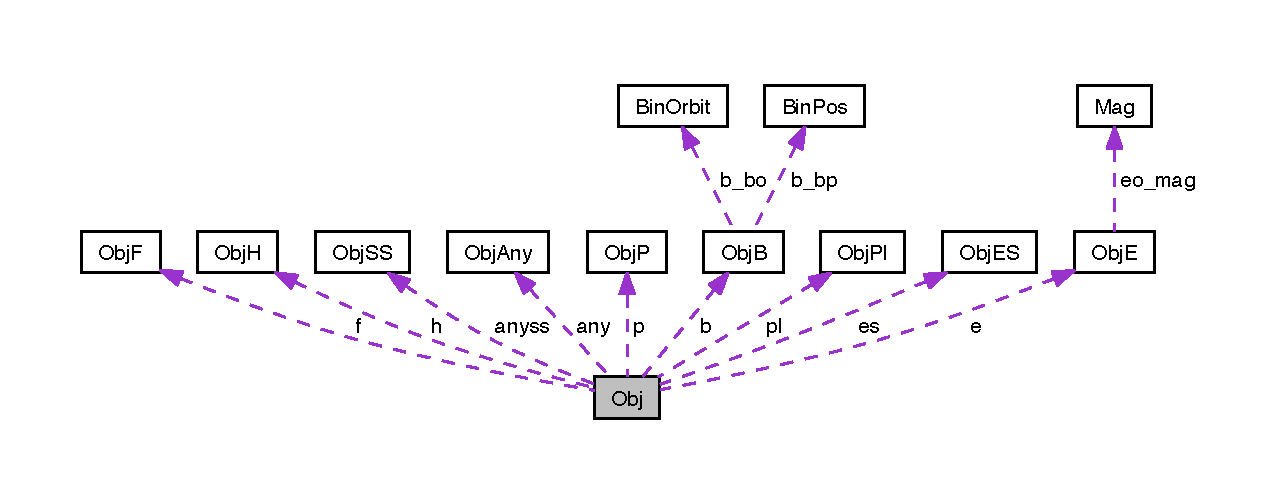
\includegraphics[width=350pt]{union_obj__coll__graph}
\end{center}
\end{figure}
\subsection*{Data Fields}
\begin{DoxyCompactItemize}
\item 
\hyperlink{struct_obj_any}{Obj\-Any} \hyperlink{union_obj_a3be70e47b7e45f1e509c5cb14b0b78ff}{any}
\item 
\hyperlink{struct_obj_s_s}{Obj\-S\-S} \hyperlink{union_obj_aa005251ef147fd79203485f59d44839a}{anyss}
\item 
\hyperlink{struct_obj_pl}{Obj\-Pl} \hyperlink{union_obj_a85c3757106e1ff2302aa87006eebc31e}{pl}
\item 
\hyperlink{struct_obj_f}{Obj\-F} \hyperlink{union_obj_a208e4a5dfb78b3b3e667b481694b155c}{f}
\item 
\hyperlink{struct_obj_b}{Obj\-B} \hyperlink{union_obj_acb73b50da4a37f11692fc44ef563a227}{b}
\item 
\hyperlink{struct_obj_e}{Obj\-E} \hyperlink{union_obj_ad9cbacafcfa52192f9e810aadd170941}{e}
\item 
\hyperlink{struct_obj_h}{Obj\-H} \hyperlink{union_obj_abbef64a85f55d6aaff88d47e2a9dc883}{h}
\item 
\hyperlink{struct_obj_p}{Obj\-P} \hyperlink{union_obj_a698977a8ec8db73cf433246f32a1c88c}{p}
\item 
\hyperlink{struct_obj_e_s}{Obj\-E\-S} \hyperlink{union_obj_abde2a9cfca01fb66e841ab82e343b710}{es}
\end{DoxyCompactItemize}


\subsection{Detailed Description}


Definition at line 332 of file astro.\-h.



\subsection{Field Documentation}
\hypertarget{union_obj_a3be70e47b7e45f1e509c5cb14b0b78ff}{\index{Obj@{Obj}!any@{any}}
\index{any@{any}!Obj@{Obj}}
\subsubsection[{any}]{\setlength{\rightskip}{0pt plus 5cm}{\bf Obj\-Any} Obj\-::any}}\label{union_obj_a3be70e47b7e45f1e509c5cb14b0b78ff}


Definition at line 333 of file astro.\-h.

\hypertarget{union_obj_aa005251ef147fd79203485f59d44839a}{\index{Obj@{Obj}!anyss@{anyss}}
\index{anyss@{anyss}!Obj@{Obj}}
\subsubsection[{anyss}]{\setlength{\rightskip}{0pt plus 5cm}{\bf Obj\-S\-S} Obj\-::anyss}}\label{union_obj_aa005251ef147fd79203485f59d44839a}


Definition at line 334 of file astro.\-h.

\hypertarget{union_obj_acb73b50da4a37f11692fc44ef563a227}{\index{Obj@{Obj}!b@{b}}
\index{b@{b}!Obj@{Obj}}
\subsubsection[{b}]{\setlength{\rightskip}{0pt plus 5cm}{\bf Obj\-B} Obj\-::b}}\label{union_obj_acb73b50da4a37f11692fc44ef563a227}


Definition at line 337 of file astro.\-h.

\hypertarget{union_obj_ad9cbacafcfa52192f9e810aadd170941}{\index{Obj@{Obj}!e@{e}}
\index{e@{e}!Obj@{Obj}}
\subsubsection[{e}]{\setlength{\rightskip}{0pt plus 5cm}{\bf Obj\-E} Obj\-::e}}\label{union_obj_ad9cbacafcfa52192f9e810aadd170941}


Definition at line 338 of file astro.\-h.

\hypertarget{union_obj_abde2a9cfca01fb66e841ab82e343b710}{\index{Obj@{Obj}!es@{es}}
\index{es@{es}!Obj@{Obj}}
\subsubsection[{es}]{\setlength{\rightskip}{0pt plus 5cm}{\bf Obj\-E\-S} Obj\-::es}}\label{union_obj_abde2a9cfca01fb66e841ab82e343b710}


Definition at line 341 of file astro.\-h.

\hypertarget{union_obj_a208e4a5dfb78b3b3e667b481694b155c}{\index{Obj@{Obj}!f@{f}}
\index{f@{f}!Obj@{Obj}}
\subsubsection[{f}]{\setlength{\rightskip}{0pt plus 5cm}{\bf Obj\-F} Obj\-::f}}\label{union_obj_a208e4a5dfb78b3b3e667b481694b155c}


Definition at line 336 of file astro.\-h.

\hypertarget{union_obj_abbef64a85f55d6aaff88d47e2a9dc883}{\index{Obj@{Obj}!h@{h}}
\index{h@{h}!Obj@{Obj}}
\subsubsection[{h}]{\setlength{\rightskip}{0pt plus 5cm}{\bf Obj\-H} Obj\-::h}}\label{union_obj_abbef64a85f55d6aaff88d47e2a9dc883}


Definition at line 339 of file astro.\-h.

\hypertarget{union_obj_a698977a8ec8db73cf433246f32a1c88c}{\index{Obj@{Obj}!p@{p}}
\index{p@{p}!Obj@{Obj}}
\subsubsection[{p}]{\setlength{\rightskip}{0pt plus 5cm}{\bf Obj\-P} Obj\-::p}}\label{union_obj_a698977a8ec8db73cf433246f32a1c88c}


Definition at line 340 of file astro.\-h.

\hypertarget{union_obj_a85c3757106e1ff2302aa87006eebc31e}{\index{Obj@{Obj}!pl@{pl}}
\index{pl@{pl}!Obj@{Obj}}
\subsubsection[{pl}]{\setlength{\rightskip}{0pt plus 5cm}{\bf Obj\-Pl} Obj\-::pl}}\label{union_obj_a85c3757106e1ff2302aa87006eebc31e}


Definition at line 335 of file astro.\-h.



The documentation for this union was generated from the following file\-:\begin{DoxyCompactItemize}
\item 
libastro/\hyperlink{astro_8h}{astro.\-h}\end{DoxyCompactItemize}

\hypertarget{struct_obj_any}{\section{Obj\-Any Struct Reference}
\label{struct_obj_any}\index{Obj\-Any@{Obj\-Any}}
}


{\ttfamily \#include $<$astro.\-h$>$}

\subsection*{Data Fields}
\begin{DoxyCompactItemize}
\item 
\hyperlink{struct_obj_any_a7f2257d4bcaa761474eebc5712819293}{O\-B\-J\-\_\-\-C\-O\-M\-M\-O\-N\-\_\-\-F\-L\-D\-S}
\end{DoxyCompactItemize}


\subsection{Detailed Description}


Definition at line 168 of file astro.\-h.



\subsection{Field Documentation}
\hypertarget{struct_obj_any_a7f2257d4bcaa761474eebc5712819293}{\index{Obj\-Any@{Obj\-Any}!O\-B\-J\-\_\-\-C\-O\-M\-M\-O\-N\-\_\-\-F\-L\-D\-S@{O\-B\-J\-\_\-\-C\-O\-M\-M\-O\-N\-\_\-\-F\-L\-D\-S}}
\index{O\-B\-J\-\_\-\-C\-O\-M\-M\-O\-N\-\_\-\-F\-L\-D\-S@{O\-B\-J\-\_\-\-C\-O\-M\-M\-O\-N\-\_\-\-F\-L\-D\-S}!ObjAny@{Obj\-Any}}
\subsubsection[{O\-B\-J\-\_\-\-C\-O\-M\-M\-O\-N\-\_\-\-F\-L\-D\-S}]{\setlength{\rightskip}{0pt plus 5cm}Obj\-Any\-::\-O\-B\-J\-\_\-\-C\-O\-M\-M\-O\-N\-\_\-\-F\-L\-D\-S}}\label{struct_obj_any_a7f2257d4bcaa761474eebc5712819293}


Definition at line 169 of file astro.\-h.



The documentation for this struct was generated from the following file\-:\begin{DoxyCompactItemize}
\item 
libastro/\hyperlink{astro_8h}{astro.\-h}\end{DoxyCompactItemize}

\hypertarget{struct_obj_b}{\section{Obj\-B Struct Reference}
\label{struct_obj_b}\index{Obj\-B@{Obj\-B}}
}


{\ttfamily \#include $<$astro.\-h$>$}



Collaboration diagram for Obj\-B\-:
\nopagebreak
\begin{figure}[H]
\begin{center}
\leavevmode
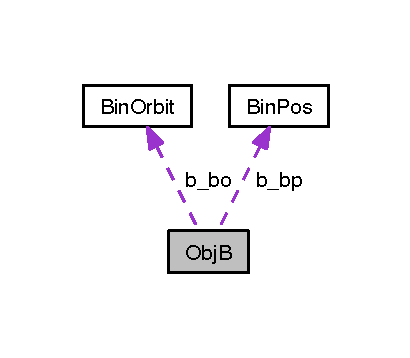
\includegraphics[width=197pt]{struct_obj_b__coll__graph}
\end{center}
\end{figure}
\subsection*{Data Fields}
\begin{DoxyCompactItemize}
\item 
\hyperlink{struct_obj_b_a1a35d318e044b682941c0030c856dbed}{O\-B\-J\-\_\-\-C\-O\-M\-M\-O\-N\-\_\-\-F\-L\-D\-S}
\item 
\hyperlink{struct_obj_b_aa756c8c241e67339e273e8d3a5215e1c}{O\-B\-J\-\_\-\-F\-I\-X\-E\-D\-\_\-\-F\-L\-D\-S}
\item 
\hyperlink{astro_8h_a0c8186d9b9b7880309c27230bbb5e69d}{byte} \hyperlink{struct_obj_b_a88427754346c50b349a50d472946644b}{b\-\_\-2compute}
\item 
\hyperlink{astro_8h_a0c8186d9b9b7880309c27230bbb5e69d}{byte} \hyperlink{struct_obj_b_a3314e81ed5e1a63b2bc9c91aa05161fe}{b\-\_\-nbp}
\item 
short \hyperlink{struct_obj_b_a16a3be87a937ea9c4387056771aa0add}{b\-\_\-2mag}
\item 
char \hyperlink{struct_obj_b_a4e3335adf18f2b6140f6f92e3e78a350}{b\-\_\-2spect} \mbox{[}2\mbox{]}
\item 
\begin{tabbing}
xx\=xx\=xx\=xx\=xx\=xx\=xx\=xx\=xx\=\kill
union \{\\
\>\hyperlink{struct_bin_orbit}{BinOrbit} \hyperlink{struct_obj_b_a5bc226e04f07466871691875560c91a9}{b\_bo}\\
\>\hyperlink{struct_bin_pos}{BinPos} \hyperlink{struct_obj_b_a7511eaac1e5e7c4f30ebb1cc5ba546a2}{b\_bp} \mbox{[}\hyperlink{astro_8h_ae71358c16a25f35949f4b21cb745790f}{MAXBINPOS}\mbox{]}\\
\} \hyperlink{struct_obj_b_a5a002e40b447bb980bb3375c58ab7d48}{u}\\

\end{tabbing}\end{DoxyCompactItemize}


\subsection{Detailed Description}


Definition at line 214 of file astro.\-h.



\subsection{Field Documentation}
\hypertarget{struct_obj_b_a88427754346c50b349a50d472946644b}{\index{Obj\-B@{Obj\-B}!b\-\_\-2compute@{b\-\_\-2compute}}
\index{b\-\_\-2compute@{b\-\_\-2compute}!ObjB@{Obj\-B}}
\subsubsection[{b\-\_\-2compute}]{\setlength{\rightskip}{0pt plus 5cm}{\bf byte} Obj\-B\-::b\-\_\-2compute}}\label{struct_obj_b_a88427754346c50b349a50d472946644b}


Definition at line 218 of file astro.\-h.

\hypertarget{struct_obj_b_a16a3be87a937ea9c4387056771aa0add}{\index{Obj\-B@{Obj\-B}!b\-\_\-2mag@{b\-\_\-2mag}}
\index{b\-\_\-2mag@{b\-\_\-2mag}!ObjB@{Obj\-B}}
\subsubsection[{b\-\_\-2mag}]{\setlength{\rightskip}{0pt plus 5cm}short Obj\-B\-::b\-\_\-2mag}}\label{struct_obj_b_a16a3be87a937ea9c4387056771aa0add}


Definition at line 220 of file astro.\-h.

\hypertarget{struct_obj_b_a4e3335adf18f2b6140f6f92e3e78a350}{\index{Obj\-B@{Obj\-B}!b\-\_\-2spect@{b\-\_\-2spect}}
\index{b\-\_\-2spect@{b\-\_\-2spect}!ObjB@{Obj\-B}}
\subsubsection[{b\-\_\-2spect}]{\setlength{\rightskip}{0pt plus 5cm}char Obj\-B\-::b\-\_\-2spect\mbox{[}2\mbox{]}}}\label{struct_obj_b_a4e3335adf18f2b6140f6f92e3e78a350}


Definition at line 221 of file astro.\-h.

\hypertarget{struct_obj_b_a5bc226e04f07466871691875560c91a9}{\index{Obj\-B@{Obj\-B}!b\-\_\-bo@{b\-\_\-bo}}
\index{b\-\_\-bo@{b\-\_\-bo}!ObjB@{Obj\-B}}
\subsubsection[{b\-\_\-bo}]{\setlength{\rightskip}{0pt plus 5cm}{\bf Bin\-Orbit} Obj\-B\-::b\-\_\-bo}}\label{struct_obj_b_a5bc226e04f07466871691875560c91a9}


Definition at line 225 of file astro.\-h.

\hypertarget{struct_obj_b_a7511eaac1e5e7c4f30ebb1cc5ba546a2}{\index{Obj\-B@{Obj\-B}!b\-\_\-bp@{b\-\_\-bp}}
\index{b\-\_\-bp@{b\-\_\-bp}!ObjB@{Obj\-B}}
\subsubsection[{b\-\_\-bp}]{\setlength{\rightskip}{0pt plus 5cm}{\bf Bin\-Pos} Obj\-B\-::b\-\_\-bp\mbox{[}{\bf M\-A\-X\-B\-I\-N\-P\-O\-S}\mbox{]}}}\label{struct_obj_b_a7511eaac1e5e7c4f30ebb1cc5ba546a2}


Definition at line 226 of file astro.\-h.

\hypertarget{struct_obj_b_a3314e81ed5e1a63b2bc9c91aa05161fe}{\index{Obj\-B@{Obj\-B}!b\-\_\-nbp@{b\-\_\-nbp}}
\index{b\-\_\-nbp@{b\-\_\-nbp}!ObjB@{Obj\-B}}
\subsubsection[{b\-\_\-nbp}]{\setlength{\rightskip}{0pt plus 5cm}{\bf byte} Obj\-B\-::b\-\_\-nbp}}\label{struct_obj_b_a3314e81ed5e1a63b2bc9c91aa05161fe}


Definition at line 219 of file astro.\-h.

\hypertarget{struct_obj_b_a1a35d318e044b682941c0030c856dbed}{\index{Obj\-B@{Obj\-B}!O\-B\-J\-\_\-\-C\-O\-M\-M\-O\-N\-\_\-\-F\-L\-D\-S@{O\-B\-J\-\_\-\-C\-O\-M\-M\-O\-N\-\_\-\-F\-L\-D\-S}}
\index{O\-B\-J\-\_\-\-C\-O\-M\-M\-O\-N\-\_\-\-F\-L\-D\-S@{O\-B\-J\-\_\-\-C\-O\-M\-M\-O\-N\-\_\-\-F\-L\-D\-S}!ObjB@{Obj\-B}}
\subsubsection[{O\-B\-J\-\_\-\-C\-O\-M\-M\-O\-N\-\_\-\-F\-L\-D\-S}]{\setlength{\rightskip}{0pt plus 5cm}Obj\-B\-::\-O\-B\-J\-\_\-\-C\-O\-M\-M\-O\-N\-\_\-\-F\-L\-D\-S}}\label{struct_obj_b_a1a35d318e044b682941c0030c856dbed}


Definition at line 215 of file astro.\-h.

\hypertarget{struct_obj_b_aa756c8c241e67339e273e8d3a5215e1c}{\index{Obj\-B@{Obj\-B}!O\-B\-J\-\_\-\-F\-I\-X\-E\-D\-\_\-\-F\-L\-D\-S@{O\-B\-J\-\_\-\-F\-I\-X\-E\-D\-\_\-\-F\-L\-D\-S}}
\index{O\-B\-J\-\_\-\-F\-I\-X\-E\-D\-\_\-\-F\-L\-D\-S@{O\-B\-J\-\_\-\-F\-I\-X\-E\-D\-\_\-\-F\-L\-D\-S}!ObjB@{Obj\-B}}
\subsubsection[{O\-B\-J\-\_\-\-F\-I\-X\-E\-D\-\_\-\-F\-L\-D\-S}]{\setlength{\rightskip}{0pt plus 5cm}Obj\-B\-::\-O\-B\-J\-\_\-\-F\-I\-X\-E\-D\-\_\-\-F\-L\-D\-S}}\label{struct_obj_b_aa756c8c241e67339e273e8d3a5215e1c}


Definition at line 216 of file astro.\-h.

\hypertarget{struct_obj_b_a5a002e40b447bb980bb3375c58ab7d48}{\index{Obj\-B@{Obj\-B}!u@{u}}
\index{u@{u}!ObjB@{Obj\-B}}
\subsubsection[{u}]{\setlength{\rightskip}{0pt plus 5cm}union \{ ... \}   Obj\-B\-::u}}\label{struct_obj_b_a5a002e40b447bb980bb3375c58ab7d48}


The documentation for this struct was generated from the following file\-:\begin{DoxyCompactItemize}
\item 
libastro/\hyperlink{astro_8h}{astro.\-h}\end{DoxyCompactItemize}

\hypertarget{struct_obj_e}{\section{Obj\-E Struct Reference}
\label{struct_obj_e}\index{Obj\-E@{Obj\-E}}
}


{\ttfamily \#include $<$astro.\-h$>$}



Collaboration diagram for Obj\-E\-:
\nopagebreak
\begin{figure}[H]
\begin{center}
\leavevmode
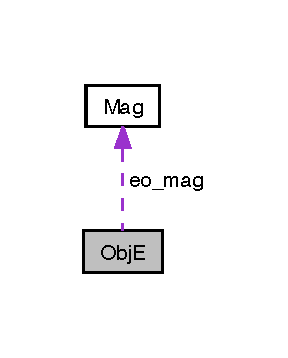
\includegraphics[width=138pt]{struct_obj_e__coll__graph}
\end{center}
\end{figure}
\subsection*{Data Fields}
\begin{DoxyCompactItemize}
\item 
\hyperlink{struct_obj_e_a99f83e9c2a725f3ac18aa4fa6a78b4c6}{O\-B\-J\-\_\-\-S\-O\-L\-S\-Y\-S\-\_\-\-F\-L\-D\-S}
\item 
float \hyperlink{struct_obj_e_ae56287dddc0ff0cee17a0c320cb231c4}{eo\-\_\-inc}
\item 
float \hyperlink{struct_obj_e_a705d0e32e827fb82f140f44259192a1d}{eo\-\_\-\-Om}
\item 
float \hyperlink{struct_obj_e_a141d2d2f867c980b6659d2107929503a}{eo\-\_\-om}
\item 
float \hyperlink{struct_obj_e_ac41c81ba9ecc8a7c26a386322dea5f55}{eo\-\_\-a}
\item 
float \hyperlink{struct_obj_e_abf1b3b9093196f05339af6b2c103b452}{eo\-\_\-\-M}
\item 
float \hyperlink{struct_obj_e_aa2b3a65ada0f743f8b09ef8794298fe7}{eo\-\_\-size}
\item 
float \hyperlink{struct_obj_e_a645f746b4ddffb8d9d4413bde196a12a}{eo\-\_\-startok}
\item 
float \hyperlink{struct_obj_e_a32f5f29577591f4c0565f678e2564062}{eo\-\_\-endok}
\item 
double \hyperlink{struct_obj_e_a0405fd0f0db7d32fa17673b2e7310739}{eo\-\_\-e}
\item 
double \hyperlink{struct_obj_e_a2b47b1a9a359291e845e24d6fdd0b389}{eo\-\_\-cepoch}
\item 
double \hyperlink{struct_obj_e_a616f7a6b3e8f5be54b889ed4127f51e4}{eo\-\_\-epoch}
\item 
\hyperlink{struct_mag}{Mag} \hyperlink{struct_obj_e_af226a2ba02b4f5af8848bbcf601272bc}{eo\-\_\-mag}
\end{DoxyCompactItemize}


\subsection{Detailed Description}


Definition at line 256 of file astro.\-h.



\subsection{Field Documentation}
\hypertarget{struct_obj_e_ac41c81ba9ecc8a7c26a386322dea5f55}{\index{Obj\-E@{Obj\-E}!eo\-\_\-a@{eo\-\_\-a}}
\index{eo\-\_\-a@{eo\-\_\-a}!ObjE@{Obj\-E}}
\subsubsection[{eo\-\_\-a}]{\setlength{\rightskip}{0pt plus 5cm}float Obj\-E\-::eo\-\_\-a}}\label{struct_obj_e_ac41c81ba9ecc8a7c26a386322dea5f55}


Definition at line 261 of file astro.\-h.

\hypertarget{struct_obj_e_a2b47b1a9a359291e845e24d6fdd0b389}{\index{Obj\-E@{Obj\-E}!eo\-\_\-cepoch@{eo\-\_\-cepoch}}
\index{eo\-\_\-cepoch@{eo\-\_\-cepoch}!ObjE@{Obj\-E}}
\subsubsection[{eo\-\_\-cepoch}]{\setlength{\rightskip}{0pt plus 5cm}double Obj\-E\-::eo\-\_\-cepoch}}\label{struct_obj_e_a2b47b1a9a359291e845e24d6fdd0b389}


Definition at line 267 of file astro.\-h.

\hypertarget{struct_obj_e_a0405fd0f0db7d32fa17673b2e7310739}{\index{Obj\-E@{Obj\-E}!eo\-\_\-e@{eo\-\_\-e}}
\index{eo\-\_\-e@{eo\-\_\-e}!ObjE@{Obj\-E}}
\subsubsection[{eo\-\_\-e}]{\setlength{\rightskip}{0pt plus 5cm}double Obj\-E\-::eo\-\_\-e}}\label{struct_obj_e_a0405fd0f0db7d32fa17673b2e7310739}


Definition at line 266 of file astro.\-h.

\hypertarget{struct_obj_e_a32f5f29577591f4c0565f678e2564062}{\index{Obj\-E@{Obj\-E}!eo\-\_\-endok@{eo\-\_\-endok}}
\index{eo\-\_\-endok@{eo\-\_\-endok}!ObjE@{Obj\-E}}
\subsubsection[{eo\-\_\-endok}]{\setlength{\rightskip}{0pt plus 5cm}float Obj\-E\-::eo\-\_\-endok}}\label{struct_obj_e_a32f5f29577591f4c0565f678e2564062}


Definition at line 265 of file astro.\-h.

\hypertarget{struct_obj_e_a616f7a6b3e8f5be54b889ed4127f51e4}{\index{Obj\-E@{Obj\-E}!eo\-\_\-epoch@{eo\-\_\-epoch}}
\index{eo\-\_\-epoch@{eo\-\_\-epoch}!ObjE@{Obj\-E}}
\subsubsection[{eo\-\_\-epoch}]{\setlength{\rightskip}{0pt plus 5cm}double Obj\-E\-::eo\-\_\-epoch}}\label{struct_obj_e_a616f7a6b3e8f5be54b889ed4127f51e4}


Definition at line 268 of file astro.\-h.

\hypertarget{struct_obj_e_ae56287dddc0ff0cee17a0c320cb231c4}{\index{Obj\-E@{Obj\-E}!eo\-\_\-inc@{eo\-\_\-inc}}
\index{eo\-\_\-inc@{eo\-\_\-inc}!ObjE@{Obj\-E}}
\subsubsection[{eo\-\_\-inc}]{\setlength{\rightskip}{0pt plus 5cm}float Obj\-E\-::eo\-\_\-inc}}\label{struct_obj_e_ae56287dddc0ff0cee17a0c320cb231c4}


Definition at line 258 of file astro.\-h.

\hypertarget{struct_obj_e_abf1b3b9093196f05339af6b2c103b452}{\index{Obj\-E@{Obj\-E}!eo\-\_\-\-M@{eo\-\_\-\-M}}
\index{eo\-\_\-\-M@{eo\-\_\-\-M}!ObjE@{Obj\-E}}
\subsubsection[{eo\-\_\-\-M}]{\setlength{\rightskip}{0pt plus 5cm}float Obj\-E\-::eo\-\_\-\-M}}\label{struct_obj_e_abf1b3b9093196f05339af6b2c103b452}


Definition at line 262 of file astro.\-h.

\hypertarget{struct_obj_e_af226a2ba02b4f5af8848bbcf601272bc}{\index{Obj\-E@{Obj\-E}!eo\-\_\-mag@{eo\-\_\-mag}}
\index{eo\-\_\-mag@{eo\-\_\-mag}!ObjE@{Obj\-E}}
\subsubsection[{eo\-\_\-mag}]{\setlength{\rightskip}{0pt plus 5cm}{\bf Mag} Obj\-E\-::eo\-\_\-mag}}\label{struct_obj_e_af226a2ba02b4f5af8848bbcf601272bc}


Definition at line 269 of file astro.\-h.

\hypertarget{struct_obj_e_a705d0e32e827fb82f140f44259192a1d}{\index{Obj\-E@{Obj\-E}!eo\-\_\-\-Om@{eo\-\_\-\-Om}}
\index{eo\-\_\-\-Om@{eo\-\_\-\-Om}!ObjE@{Obj\-E}}
\subsubsection[{eo\-\_\-\-Om}]{\setlength{\rightskip}{0pt plus 5cm}float Obj\-E\-::eo\-\_\-\-Om}}\label{struct_obj_e_a705d0e32e827fb82f140f44259192a1d}


Definition at line 259 of file astro.\-h.

\hypertarget{struct_obj_e_a141d2d2f867c980b6659d2107929503a}{\index{Obj\-E@{Obj\-E}!eo\-\_\-om@{eo\-\_\-om}}
\index{eo\-\_\-om@{eo\-\_\-om}!ObjE@{Obj\-E}}
\subsubsection[{eo\-\_\-om}]{\setlength{\rightskip}{0pt plus 5cm}float Obj\-E\-::eo\-\_\-om}}\label{struct_obj_e_a141d2d2f867c980b6659d2107929503a}


Definition at line 260 of file astro.\-h.

\hypertarget{struct_obj_e_aa2b3a65ada0f743f8b09ef8794298fe7}{\index{Obj\-E@{Obj\-E}!eo\-\_\-size@{eo\-\_\-size}}
\index{eo\-\_\-size@{eo\-\_\-size}!ObjE@{Obj\-E}}
\subsubsection[{eo\-\_\-size}]{\setlength{\rightskip}{0pt plus 5cm}float Obj\-E\-::eo\-\_\-size}}\label{struct_obj_e_aa2b3a65ada0f743f8b09ef8794298fe7}


Definition at line 263 of file astro.\-h.

\hypertarget{struct_obj_e_a645f746b4ddffb8d9d4413bde196a12a}{\index{Obj\-E@{Obj\-E}!eo\-\_\-startok@{eo\-\_\-startok}}
\index{eo\-\_\-startok@{eo\-\_\-startok}!ObjE@{Obj\-E}}
\subsubsection[{eo\-\_\-startok}]{\setlength{\rightskip}{0pt plus 5cm}float Obj\-E\-::eo\-\_\-startok}}\label{struct_obj_e_a645f746b4ddffb8d9d4413bde196a12a}


Definition at line 264 of file astro.\-h.

\hypertarget{struct_obj_e_a99f83e9c2a725f3ac18aa4fa6a78b4c6}{\index{Obj\-E@{Obj\-E}!O\-B\-J\-\_\-\-S\-O\-L\-S\-Y\-S\-\_\-\-F\-L\-D\-S@{O\-B\-J\-\_\-\-S\-O\-L\-S\-Y\-S\-\_\-\-F\-L\-D\-S}}
\index{O\-B\-J\-\_\-\-S\-O\-L\-S\-Y\-S\-\_\-\-F\-L\-D\-S@{O\-B\-J\-\_\-\-S\-O\-L\-S\-Y\-S\-\_\-\-F\-L\-D\-S}!ObjE@{Obj\-E}}
\subsubsection[{O\-B\-J\-\_\-\-S\-O\-L\-S\-Y\-S\-\_\-\-F\-L\-D\-S}]{\setlength{\rightskip}{0pt plus 5cm}Obj\-E\-::\-O\-B\-J\-\_\-\-S\-O\-L\-S\-Y\-S\-\_\-\-F\-L\-D\-S}}\label{struct_obj_e_a99f83e9c2a725f3ac18aa4fa6a78b4c6}


Definition at line 257 of file astro.\-h.



The documentation for this struct was generated from the following file\-:\begin{DoxyCompactItemize}
\item 
libastro/\hyperlink{astro_8h}{astro.\-h}\end{DoxyCompactItemize}

\hypertarget{struct_obj_e_s}{\section{Obj\-E\-S Struct Reference}
\label{struct_obj_e_s}\index{Obj\-E\-S@{Obj\-E\-S}}
}


{\ttfamily \#include $<$astro.\-h$>$}

\subsection*{Data Fields}
\begin{DoxyCompactItemize}
\item 
\hyperlink{struct_obj_e_s_aa17c09f5e88fab7e6a51c49354bb02ee}{O\-B\-J\-\_\-\-C\-O\-M\-M\-O\-N\-\_\-\-F\-L\-D\-S}
\item 
double \hyperlink{struct_obj_e_s_a802b004e0f70e92b5f802e2180f8e148}{eso\-\_\-epoch}
\item 
double \hyperlink{struct_obj_e_s_a0b9468f1fb373568988b87602681a7a1}{eso\-\_\-n}
\item 
float \hyperlink{struct_obj_e_s_ac838c1e7532b7f21df767d8592dcfc08}{eso\-\_\-startok}
\item 
float \hyperlink{struct_obj_e_s_acdad5e0584580a009d4df491f5ddcaa3}{eso\-\_\-endok}
\item 
float \hyperlink{struct_obj_e_s_ae8b1d0cd54db2151a4f3abce93867e34}{eso\-\_\-inc}
\item 
float \hyperlink{struct_obj_e_s_a2706cc4697ba62259e2c8d0a5355d983}{eso\-\_\-raan}
\item 
float \hyperlink{struct_obj_e_s_a4d259cf59761ca0815135a61a8c27fa7}{eso\-\_\-e}
\item 
float \hyperlink{struct_obj_e_s_ac284ba51510c470c5672dc49f72777d6}{eso\-\_\-ap}
\item 
float \hyperlink{struct_obj_e_s_ab1e0b35f063c6e34fa2a8e9bd917eecd}{eso\-\_\-\-M}
\item 
float \hyperlink{struct_obj_e_s_ad784c67228eff476b3ba6f807534889a}{eso\-\_\-decay}
\item 
float \hyperlink{struct_obj_e_s_a52ee31a4760f42b6cd3d3a135b432ddd}{eso\-\_\-drag}
\item 
int \hyperlink{struct_obj_e_s_a5447658f274c3195b450ee8ba9249590}{eso\-\_\-orbit}
\item 
float \hyperlink{struct_obj_e_s_a754520e026b1784fa73a11798ca0682f}{ess\-\_\-elev}
\item 
float \hyperlink{struct_obj_e_s_aa99b244fa218d755675be8a6bd4d50fb}{ess\-\_\-range}
\item 
float \hyperlink{struct_obj_e_s_a5fc85c3154a0491477936c63f7399664}{ess\-\_\-rangev}
\item 
float \hyperlink{struct_obj_e_s_a21073da516913e1888857e168ec25bf3}{ess\-\_\-sublat}
\item 
float \hyperlink{struct_obj_e_s_aea3fddbd7be1bbcbb13c6f8f1e468a6f}{ess\-\_\-sublng}
\item 
int \hyperlink{struct_obj_e_s_ac6d7c45b158ba372b583c2fe679f87f9}{ess\-\_\-eclipsed}
\end{DoxyCompactItemize}


\subsection{Detailed Description}


Definition at line 304 of file astro.\-h.



\subsection{Field Documentation}
\hypertarget{struct_obj_e_s_ac284ba51510c470c5672dc49f72777d6}{\index{Obj\-E\-S@{Obj\-E\-S}!eso\-\_\-ap@{eso\-\_\-ap}}
\index{eso\-\_\-ap@{eso\-\_\-ap}!ObjES@{Obj\-E\-S}}
\subsubsection[{eso\-\_\-ap}]{\setlength{\rightskip}{0pt plus 5cm}float Obj\-E\-S\-::eso\-\_\-ap}}\label{struct_obj_e_s_ac284ba51510c470c5672dc49f72777d6}


Definition at line 317 of file astro.\-h.

\hypertarget{struct_obj_e_s_ad784c67228eff476b3ba6f807534889a}{\index{Obj\-E\-S@{Obj\-E\-S}!eso\-\_\-decay@{eso\-\_\-decay}}
\index{eso\-\_\-decay@{eso\-\_\-decay}!ObjES@{Obj\-E\-S}}
\subsubsection[{eso\-\_\-decay}]{\setlength{\rightskip}{0pt plus 5cm}float Obj\-E\-S\-::eso\-\_\-decay}}\label{struct_obj_e_s_ad784c67228eff476b3ba6f807534889a}


Definition at line 319 of file astro.\-h.

\hypertarget{struct_obj_e_s_a52ee31a4760f42b6cd3d3a135b432ddd}{\index{Obj\-E\-S@{Obj\-E\-S}!eso\-\_\-drag@{eso\-\_\-drag}}
\index{eso\-\_\-drag@{eso\-\_\-drag}!ObjES@{Obj\-E\-S}}
\subsubsection[{eso\-\_\-drag}]{\setlength{\rightskip}{0pt plus 5cm}float Obj\-E\-S\-::eso\-\_\-drag}}\label{struct_obj_e_s_a52ee31a4760f42b6cd3d3a135b432ddd}


Definition at line 320 of file astro.\-h.

\hypertarget{struct_obj_e_s_a4d259cf59761ca0815135a61a8c27fa7}{\index{Obj\-E\-S@{Obj\-E\-S}!eso\-\_\-e@{eso\-\_\-e}}
\index{eso\-\_\-e@{eso\-\_\-e}!ObjES@{Obj\-E\-S}}
\subsubsection[{eso\-\_\-e}]{\setlength{\rightskip}{0pt plus 5cm}float Obj\-E\-S\-::eso\-\_\-e}}\label{struct_obj_e_s_a4d259cf59761ca0815135a61a8c27fa7}


Definition at line 316 of file astro.\-h.

\hypertarget{struct_obj_e_s_acdad5e0584580a009d4df491f5ddcaa3}{\index{Obj\-E\-S@{Obj\-E\-S}!eso\-\_\-endok@{eso\-\_\-endok}}
\index{eso\-\_\-endok@{eso\-\_\-endok}!ObjES@{Obj\-E\-S}}
\subsubsection[{eso\-\_\-endok}]{\setlength{\rightskip}{0pt plus 5cm}float Obj\-E\-S\-::eso\-\_\-endok}}\label{struct_obj_e_s_acdad5e0584580a009d4df491f5ddcaa3}


Definition at line 313 of file astro.\-h.

\hypertarget{struct_obj_e_s_a802b004e0f70e92b5f802e2180f8e148}{\index{Obj\-E\-S@{Obj\-E\-S}!eso\-\_\-epoch@{eso\-\_\-epoch}}
\index{eso\-\_\-epoch@{eso\-\_\-epoch}!ObjES@{Obj\-E\-S}}
\subsubsection[{eso\-\_\-epoch}]{\setlength{\rightskip}{0pt plus 5cm}double Obj\-E\-S\-::eso\-\_\-epoch}}\label{struct_obj_e_s_a802b004e0f70e92b5f802e2180f8e148}


Definition at line 306 of file astro.\-h.

\hypertarget{struct_obj_e_s_ae8b1d0cd54db2151a4f3abce93867e34}{\index{Obj\-E\-S@{Obj\-E\-S}!eso\-\_\-inc@{eso\-\_\-inc}}
\index{eso\-\_\-inc@{eso\-\_\-inc}!ObjES@{Obj\-E\-S}}
\subsubsection[{eso\-\_\-inc}]{\setlength{\rightskip}{0pt plus 5cm}float Obj\-E\-S\-::eso\-\_\-inc}}\label{struct_obj_e_s_ae8b1d0cd54db2151a4f3abce93867e34}


Definition at line 314 of file astro.\-h.

\hypertarget{struct_obj_e_s_ab1e0b35f063c6e34fa2a8e9bd917eecd}{\index{Obj\-E\-S@{Obj\-E\-S}!eso\-\_\-\-M@{eso\-\_\-\-M}}
\index{eso\-\_\-\-M@{eso\-\_\-\-M}!ObjES@{Obj\-E\-S}}
\subsubsection[{eso\-\_\-\-M}]{\setlength{\rightskip}{0pt plus 5cm}float Obj\-E\-S\-::eso\-\_\-\-M}}\label{struct_obj_e_s_ab1e0b35f063c6e34fa2a8e9bd917eecd}


Definition at line 318 of file astro.\-h.

\hypertarget{struct_obj_e_s_a0b9468f1fb373568988b87602681a7a1}{\index{Obj\-E\-S@{Obj\-E\-S}!eso\-\_\-n@{eso\-\_\-n}}
\index{eso\-\_\-n@{eso\-\_\-n}!ObjES@{Obj\-E\-S}}
\subsubsection[{eso\-\_\-n}]{\setlength{\rightskip}{0pt plus 5cm}double Obj\-E\-S\-::eso\-\_\-n}}\label{struct_obj_e_s_a0b9468f1fb373568988b87602681a7a1}


Definition at line 307 of file astro.\-h.

\hypertarget{struct_obj_e_s_a5447658f274c3195b450ee8ba9249590}{\index{Obj\-E\-S@{Obj\-E\-S}!eso\-\_\-orbit@{eso\-\_\-orbit}}
\index{eso\-\_\-orbit@{eso\-\_\-orbit}!ObjES@{Obj\-E\-S}}
\subsubsection[{eso\-\_\-orbit}]{\setlength{\rightskip}{0pt plus 5cm}int Obj\-E\-S\-::eso\-\_\-orbit}}\label{struct_obj_e_s_a5447658f274c3195b450ee8ba9249590}


Definition at line 321 of file astro.\-h.

\hypertarget{struct_obj_e_s_a2706cc4697ba62259e2c8d0a5355d983}{\index{Obj\-E\-S@{Obj\-E\-S}!eso\-\_\-raan@{eso\-\_\-raan}}
\index{eso\-\_\-raan@{eso\-\_\-raan}!ObjES@{Obj\-E\-S}}
\subsubsection[{eso\-\_\-raan}]{\setlength{\rightskip}{0pt plus 5cm}float Obj\-E\-S\-::eso\-\_\-raan}}\label{struct_obj_e_s_a2706cc4697ba62259e2c8d0a5355d983}


Definition at line 315 of file astro.\-h.

\hypertarget{struct_obj_e_s_ac838c1e7532b7f21df767d8592dcfc08}{\index{Obj\-E\-S@{Obj\-E\-S}!eso\-\_\-startok@{eso\-\_\-startok}}
\index{eso\-\_\-startok@{eso\-\_\-startok}!ObjES@{Obj\-E\-S}}
\subsubsection[{eso\-\_\-startok}]{\setlength{\rightskip}{0pt plus 5cm}float Obj\-E\-S\-::eso\-\_\-startok}}\label{struct_obj_e_s_ac838c1e7532b7f21df767d8592dcfc08}


Definition at line 312 of file astro.\-h.

\hypertarget{struct_obj_e_s_ac6d7c45b158ba372b583c2fe679f87f9}{\index{Obj\-E\-S@{Obj\-E\-S}!ess\-\_\-eclipsed@{ess\-\_\-eclipsed}}
\index{ess\-\_\-eclipsed@{ess\-\_\-eclipsed}!ObjES@{Obj\-E\-S}}
\subsubsection[{ess\-\_\-eclipsed}]{\setlength{\rightskip}{0pt plus 5cm}int Obj\-E\-S\-::ess\-\_\-eclipsed}}\label{struct_obj_e_s_ac6d7c45b158ba372b583c2fe679f87f9}


Definition at line 329 of file astro.\-h.

\hypertarget{struct_obj_e_s_a754520e026b1784fa73a11798ca0682f}{\index{Obj\-E\-S@{Obj\-E\-S}!ess\-\_\-elev@{ess\-\_\-elev}}
\index{ess\-\_\-elev@{ess\-\_\-elev}!ObjES@{Obj\-E\-S}}
\subsubsection[{ess\-\_\-elev}]{\setlength{\rightskip}{0pt plus 5cm}float Obj\-E\-S\-::ess\-\_\-elev}}\label{struct_obj_e_s_a754520e026b1784fa73a11798ca0682f}


Definition at line 324 of file astro.\-h.

\hypertarget{struct_obj_e_s_aa99b244fa218d755675be8a6bd4d50fb}{\index{Obj\-E\-S@{Obj\-E\-S}!ess\-\_\-range@{ess\-\_\-range}}
\index{ess\-\_\-range@{ess\-\_\-range}!ObjES@{Obj\-E\-S}}
\subsubsection[{ess\-\_\-range}]{\setlength{\rightskip}{0pt plus 5cm}float Obj\-E\-S\-::ess\-\_\-range}}\label{struct_obj_e_s_aa99b244fa218d755675be8a6bd4d50fb}


Definition at line 325 of file astro.\-h.

\hypertarget{struct_obj_e_s_a5fc85c3154a0491477936c63f7399664}{\index{Obj\-E\-S@{Obj\-E\-S}!ess\-\_\-rangev@{ess\-\_\-rangev}}
\index{ess\-\_\-rangev@{ess\-\_\-rangev}!ObjES@{Obj\-E\-S}}
\subsubsection[{ess\-\_\-rangev}]{\setlength{\rightskip}{0pt plus 5cm}float Obj\-E\-S\-::ess\-\_\-rangev}}\label{struct_obj_e_s_a5fc85c3154a0491477936c63f7399664}


Definition at line 326 of file astro.\-h.

\hypertarget{struct_obj_e_s_a21073da516913e1888857e168ec25bf3}{\index{Obj\-E\-S@{Obj\-E\-S}!ess\-\_\-sublat@{ess\-\_\-sublat}}
\index{ess\-\_\-sublat@{ess\-\_\-sublat}!ObjES@{Obj\-E\-S}}
\subsubsection[{ess\-\_\-sublat}]{\setlength{\rightskip}{0pt plus 5cm}float Obj\-E\-S\-::ess\-\_\-sublat}}\label{struct_obj_e_s_a21073da516913e1888857e168ec25bf3}


Definition at line 327 of file astro.\-h.

\hypertarget{struct_obj_e_s_aea3fddbd7be1bbcbb13c6f8f1e468a6f}{\index{Obj\-E\-S@{Obj\-E\-S}!ess\-\_\-sublng@{ess\-\_\-sublng}}
\index{ess\-\_\-sublng@{ess\-\_\-sublng}!ObjES@{Obj\-E\-S}}
\subsubsection[{ess\-\_\-sublng}]{\setlength{\rightskip}{0pt plus 5cm}float Obj\-E\-S\-::ess\-\_\-sublng}}\label{struct_obj_e_s_aea3fddbd7be1bbcbb13c6f8f1e468a6f}


Definition at line 328 of file astro.\-h.

\hypertarget{struct_obj_e_s_aa17c09f5e88fab7e6a51c49354bb02ee}{\index{Obj\-E\-S@{Obj\-E\-S}!O\-B\-J\-\_\-\-C\-O\-M\-M\-O\-N\-\_\-\-F\-L\-D\-S@{O\-B\-J\-\_\-\-C\-O\-M\-M\-O\-N\-\_\-\-F\-L\-D\-S}}
\index{O\-B\-J\-\_\-\-C\-O\-M\-M\-O\-N\-\_\-\-F\-L\-D\-S@{O\-B\-J\-\_\-\-C\-O\-M\-M\-O\-N\-\_\-\-F\-L\-D\-S}!ObjES@{Obj\-E\-S}}
\subsubsection[{O\-B\-J\-\_\-\-C\-O\-M\-M\-O\-N\-\_\-\-F\-L\-D\-S}]{\setlength{\rightskip}{0pt plus 5cm}Obj\-E\-S\-::\-O\-B\-J\-\_\-\-C\-O\-M\-M\-O\-N\-\_\-\-F\-L\-D\-S}}\label{struct_obj_e_s_aa17c09f5e88fab7e6a51c49354bb02ee}


Definition at line 305 of file astro.\-h.



The documentation for this struct was generated from the following file\-:\begin{DoxyCompactItemize}
\item 
libastro/\hyperlink{astro_8h}{astro.\-h}\end{DoxyCompactItemize}

\hypertarget{struct_obj_f}{\section{Obj\-F Struct Reference}
\label{struct_obj_f}\index{Obj\-F@{Obj\-F}}
}


{\ttfamily \#include $<$astro.\-h$>$}

\subsection*{Data Fields}
\begin{DoxyCompactItemize}
\item 
\hyperlink{struct_obj_f_ac06485a349b8c66de064f281140c3741}{O\-B\-J\-\_\-\-C\-O\-M\-M\-O\-N\-\_\-\-F\-L\-D\-S}
\item 
\hyperlink{struct_obj_f_a97411dd8e4c88e38ef9dd489836fe350}{O\-B\-J\-\_\-\-F\-I\-X\-E\-D\-\_\-\-F\-L\-D\-S}
\item 
\hyperlink{astro_8h_a0c8186d9b9b7880309c27230bbb5e69d}{byte} \hyperlink{struct_obj_f_a6411aff1d47e8f79b1b933e83925a249}{fo\-\_\-ratio}
\item 
\hyperlink{astro_8h_a0c8186d9b9b7880309c27230bbb5e69d}{byte} \hyperlink{struct_obj_f_a2b8b41f2c66491d316082f89072bc015}{fo\-\_\-pa}
\end{DoxyCompactItemize}


\subsection{Detailed Description}


Definition at line 179 of file astro.\-h.



\subsection{Field Documentation}
\hypertarget{struct_obj_f_a2b8b41f2c66491d316082f89072bc015}{\index{Obj\-F@{Obj\-F}!fo\-\_\-pa@{fo\-\_\-pa}}
\index{fo\-\_\-pa@{fo\-\_\-pa}!ObjF@{Obj\-F}}
\subsubsection[{fo\-\_\-pa}]{\setlength{\rightskip}{0pt plus 5cm}{\bf byte} Obj\-F\-::fo\-\_\-pa}}\label{struct_obj_f_a2b8b41f2c66491d316082f89072bc015}


Definition at line 185 of file astro.\-h.

\hypertarget{struct_obj_f_a6411aff1d47e8f79b1b933e83925a249}{\index{Obj\-F@{Obj\-F}!fo\-\_\-ratio@{fo\-\_\-ratio}}
\index{fo\-\_\-ratio@{fo\-\_\-ratio}!ObjF@{Obj\-F}}
\subsubsection[{fo\-\_\-ratio}]{\setlength{\rightskip}{0pt plus 5cm}{\bf byte} Obj\-F\-::fo\-\_\-ratio}}\label{struct_obj_f_a6411aff1d47e8f79b1b933e83925a249}


Definition at line 184 of file astro.\-h.

\hypertarget{struct_obj_f_ac06485a349b8c66de064f281140c3741}{\index{Obj\-F@{Obj\-F}!O\-B\-J\-\_\-\-C\-O\-M\-M\-O\-N\-\_\-\-F\-L\-D\-S@{O\-B\-J\-\_\-\-C\-O\-M\-M\-O\-N\-\_\-\-F\-L\-D\-S}}
\index{O\-B\-J\-\_\-\-C\-O\-M\-M\-O\-N\-\_\-\-F\-L\-D\-S@{O\-B\-J\-\_\-\-C\-O\-M\-M\-O\-N\-\_\-\-F\-L\-D\-S}!ObjF@{Obj\-F}}
\subsubsection[{O\-B\-J\-\_\-\-C\-O\-M\-M\-O\-N\-\_\-\-F\-L\-D\-S}]{\setlength{\rightskip}{0pt plus 5cm}Obj\-F\-::\-O\-B\-J\-\_\-\-C\-O\-M\-M\-O\-N\-\_\-\-F\-L\-D\-S}}\label{struct_obj_f_ac06485a349b8c66de064f281140c3741}


Definition at line 180 of file astro.\-h.

\hypertarget{struct_obj_f_a97411dd8e4c88e38ef9dd489836fe350}{\index{Obj\-F@{Obj\-F}!O\-B\-J\-\_\-\-F\-I\-X\-E\-D\-\_\-\-F\-L\-D\-S@{O\-B\-J\-\_\-\-F\-I\-X\-E\-D\-\_\-\-F\-L\-D\-S}}
\index{O\-B\-J\-\_\-\-F\-I\-X\-E\-D\-\_\-\-F\-L\-D\-S@{O\-B\-J\-\_\-\-F\-I\-X\-E\-D\-\_\-\-F\-L\-D\-S}!ObjF@{Obj\-F}}
\subsubsection[{O\-B\-J\-\_\-\-F\-I\-X\-E\-D\-\_\-\-F\-L\-D\-S}]{\setlength{\rightskip}{0pt plus 5cm}Obj\-F\-::\-O\-B\-J\-\_\-\-F\-I\-X\-E\-D\-\_\-\-F\-L\-D\-S}}\label{struct_obj_f_a97411dd8e4c88e38ef9dd489836fe350}


Definition at line 181 of file astro.\-h.



The documentation for this struct was generated from the following file\-:\begin{DoxyCompactItemize}
\item 
libastro/\hyperlink{astro_8h}{astro.\-h}\end{DoxyCompactItemize}

\hypertarget{struct_obj_h}{\section{Obj\-H Struct Reference}
\label{struct_obj_h}\index{Obj\-H@{Obj\-H}}
}


{\ttfamily \#include $<$astro.\-h$>$}

\subsection*{Data Fields}
\begin{DoxyCompactItemize}
\item 
\hyperlink{struct_obj_h_abb6e12c6ba111654831b0ace643d0e2c}{O\-B\-J\-\_\-\-S\-O\-L\-S\-Y\-S\-\_\-\-F\-L\-D\-S}
\item 
double \hyperlink{struct_obj_h_a2f0e63cb5deb63325a9df5488c1065c6}{ho\-\_\-epoch}
\item 
double \hyperlink{struct_obj_h_ad9185c53c71c2c98e49c888b72fbb716}{ho\-\_\-ep}
\item 
float \hyperlink{struct_obj_h_a09a9398b2a44b9a95d15284daa062da8}{ho\-\_\-startok}
\item 
float \hyperlink{struct_obj_h_a6058af1ea092b60bdc3e36c23429de3d}{ho\-\_\-endok}
\item 
float \hyperlink{struct_obj_h_ae6a3a975d680d5b55ffaa38cd2183476}{ho\-\_\-inc}
\item 
float \hyperlink{struct_obj_h_ad379f0625db7fcc67e51493110760de8}{ho\-\_\-\-Om}
\item 
float \hyperlink{struct_obj_h_a4a4312e20e35070f22625697e0da31ec}{ho\-\_\-om}
\item 
float \hyperlink{struct_obj_h_a71578b9d761dcb519aea89c67f87bf41}{ho\-\_\-e}
\item 
float \hyperlink{struct_obj_h_a89c7dcc10a5794cd1dc92c32a440433d}{ho\-\_\-qp}
\item 
float \hyperlink{struct_obj_h_a0d24d7f726f07bcbf17a8efd17d0fa52}{ho\-\_\-g}
\item 
float \hyperlink{struct_obj_h_a9c3656cdd0720d38c878fb01801e5fd5}{ho\-\_\-k}
\item 
float \hyperlink{struct_obj_h_a336096f873915f72ec8729ce4fe97623}{ho\-\_\-size}
\end{DoxyCompactItemize}


\subsection{Detailed Description}


Definition at line 273 of file astro.\-h.



\subsection{Field Documentation}
\hypertarget{struct_obj_h_a71578b9d761dcb519aea89c67f87bf41}{\index{Obj\-H@{Obj\-H}!ho\-\_\-e@{ho\-\_\-e}}
\index{ho\-\_\-e@{ho\-\_\-e}!ObjH@{Obj\-H}}
\subsubsection[{ho\-\_\-e}]{\setlength{\rightskip}{0pt plus 5cm}float Obj\-H\-::ho\-\_\-e}}\label{struct_obj_h_a71578b9d761dcb519aea89c67f87bf41}


Definition at line 282 of file astro.\-h.

\hypertarget{struct_obj_h_a6058af1ea092b60bdc3e36c23429de3d}{\index{Obj\-H@{Obj\-H}!ho\-\_\-endok@{ho\-\_\-endok}}
\index{ho\-\_\-endok@{ho\-\_\-endok}!ObjH@{Obj\-H}}
\subsubsection[{ho\-\_\-endok}]{\setlength{\rightskip}{0pt plus 5cm}float Obj\-H\-::ho\-\_\-endok}}\label{struct_obj_h_a6058af1ea092b60bdc3e36c23429de3d}


Definition at line 278 of file astro.\-h.

\hypertarget{struct_obj_h_ad9185c53c71c2c98e49c888b72fbb716}{\index{Obj\-H@{Obj\-H}!ho\-\_\-ep@{ho\-\_\-ep}}
\index{ho\-\_\-ep@{ho\-\_\-ep}!ObjH@{Obj\-H}}
\subsubsection[{ho\-\_\-ep}]{\setlength{\rightskip}{0pt plus 5cm}double Obj\-H\-::ho\-\_\-ep}}\label{struct_obj_h_ad9185c53c71c2c98e49c888b72fbb716}


Definition at line 276 of file astro.\-h.

\hypertarget{struct_obj_h_a2f0e63cb5deb63325a9df5488c1065c6}{\index{Obj\-H@{Obj\-H}!ho\-\_\-epoch@{ho\-\_\-epoch}}
\index{ho\-\_\-epoch@{ho\-\_\-epoch}!ObjH@{Obj\-H}}
\subsubsection[{ho\-\_\-epoch}]{\setlength{\rightskip}{0pt plus 5cm}double Obj\-H\-::ho\-\_\-epoch}}\label{struct_obj_h_a2f0e63cb5deb63325a9df5488c1065c6}


Definition at line 275 of file astro.\-h.

\hypertarget{struct_obj_h_a0d24d7f726f07bcbf17a8efd17d0fa52}{\index{Obj\-H@{Obj\-H}!ho\-\_\-g@{ho\-\_\-g}}
\index{ho\-\_\-g@{ho\-\_\-g}!ObjH@{Obj\-H}}
\subsubsection[{ho\-\_\-g}]{\setlength{\rightskip}{0pt plus 5cm}float Obj\-H\-::ho\-\_\-g}}\label{struct_obj_h_a0d24d7f726f07bcbf17a8efd17d0fa52}


Definition at line 284 of file astro.\-h.

\hypertarget{struct_obj_h_ae6a3a975d680d5b55ffaa38cd2183476}{\index{Obj\-H@{Obj\-H}!ho\-\_\-inc@{ho\-\_\-inc}}
\index{ho\-\_\-inc@{ho\-\_\-inc}!ObjH@{Obj\-H}}
\subsubsection[{ho\-\_\-inc}]{\setlength{\rightskip}{0pt plus 5cm}float Obj\-H\-::ho\-\_\-inc}}\label{struct_obj_h_ae6a3a975d680d5b55ffaa38cd2183476}


Definition at line 279 of file astro.\-h.

\hypertarget{struct_obj_h_a9c3656cdd0720d38c878fb01801e5fd5}{\index{Obj\-H@{Obj\-H}!ho\-\_\-k@{ho\-\_\-k}}
\index{ho\-\_\-k@{ho\-\_\-k}!ObjH@{Obj\-H}}
\subsubsection[{ho\-\_\-k}]{\setlength{\rightskip}{0pt plus 5cm}float Obj\-H\-::ho\-\_\-k}}\label{struct_obj_h_a9c3656cdd0720d38c878fb01801e5fd5}


Definition at line 284 of file astro.\-h.

\hypertarget{struct_obj_h_ad379f0625db7fcc67e51493110760de8}{\index{Obj\-H@{Obj\-H}!ho\-\_\-\-Om@{ho\-\_\-\-Om}}
\index{ho\-\_\-\-Om@{ho\-\_\-\-Om}!ObjH@{Obj\-H}}
\subsubsection[{ho\-\_\-\-Om}]{\setlength{\rightskip}{0pt plus 5cm}float Obj\-H\-::ho\-\_\-\-Om}}\label{struct_obj_h_ad379f0625db7fcc67e51493110760de8}


Definition at line 280 of file astro.\-h.

\hypertarget{struct_obj_h_a4a4312e20e35070f22625697e0da31ec}{\index{Obj\-H@{Obj\-H}!ho\-\_\-om@{ho\-\_\-om}}
\index{ho\-\_\-om@{ho\-\_\-om}!ObjH@{Obj\-H}}
\subsubsection[{ho\-\_\-om}]{\setlength{\rightskip}{0pt plus 5cm}float Obj\-H\-::ho\-\_\-om}}\label{struct_obj_h_a4a4312e20e35070f22625697e0da31ec}


Definition at line 281 of file astro.\-h.

\hypertarget{struct_obj_h_a89c7dcc10a5794cd1dc92c32a440433d}{\index{Obj\-H@{Obj\-H}!ho\-\_\-qp@{ho\-\_\-qp}}
\index{ho\-\_\-qp@{ho\-\_\-qp}!ObjH@{Obj\-H}}
\subsubsection[{ho\-\_\-qp}]{\setlength{\rightskip}{0pt plus 5cm}float Obj\-H\-::ho\-\_\-qp}}\label{struct_obj_h_a89c7dcc10a5794cd1dc92c32a440433d}


Definition at line 283 of file astro.\-h.

\hypertarget{struct_obj_h_a336096f873915f72ec8729ce4fe97623}{\index{Obj\-H@{Obj\-H}!ho\-\_\-size@{ho\-\_\-size}}
\index{ho\-\_\-size@{ho\-\_\-size}!ObjH@{Obj\-H}}
\subsubsection[{ho\-\_\-size}]{\setlength{\rightskip}{0pt plus 5cm}float Obj\-H\-::ho\-\_\-size}}\label{struct_obj_h_a336096f873915f72ec8729ce4fe97623}


Definition at line 285 of file astro.\-h.

\hypertarget{struct_obj_h_a09a9398b2a44b9a95d15284daa062da8}{\index{Obj\-H@{Obj\-H}!ho\-\_\-startok@{ho\-\_\-startok}}
\index{ho\-\_\-startok@{ho\-\_\-startok}!ObjH@{Obj\-H}}
\subsubsection[{ho\-\_\-startok}]{\setlength{\rightskip}{0pt plus 5cm}float Obj\-H\-::ho\-\_\-startok}}\label{struct_obj_h_a09a9398b2a44b9a95d15284daa062da8}


Definition at line 277 of file astro.\-h.

\hypertarget{struct_obj_h_abb6e12c6ba111654831b0ace643d0e2c}{\index{Obj\-H@{Obj\-H}!O\-B\-J\-\_\-\-S\-O\-L\-S\-Y\-S\-\_\-\-F\-L\-D\-S@{O\-B\-J\-\_\-\-S\-O\-L\-S\-Y\-S\-\_\-\-F\-L\-D\-S}}
\index{O\-B\-J\-\_\-\-S\-O\-L\-S\-Y\-S\-\_\-\-F\-L\-D\-S@{O\-B\-J\-\_\-\-S\-O\-L\-S\-Y\-S\-\_\-\-F\-L\-D\-S}!ObjH@{Obj\-H}}
\subsubsection[{O\-B\-J\-\_\-\-S\-O\-L\-S\-Y\-S\-\_\-\-F\-L\-D\-S}]{\setlength{\rightskip}{0pt plus 5cm}Obj\-H\-::\-O\-B\-J\-\_\-\-S\-O\-L\-S\-Y\-S\-\_\-\-F\-L\-D\-S}}\label{struct_obj_h_abb6e12c6ba111654831b0ace643d0e2c}


Definition at line 274 of file astro.\-h.



The documentation for this struct was generated from the following file\-:\begin{DoxyCompactItemize}
\item 
libastro/\hyperlink{astro_8h}{astro.\-h}\end{DoxyCompactItemize}

\hypertarget{struct_obj_p}{\section{Obj\-P Struct Reference}
\label{struct_obj_p}\index{Obj\-P@{Obj\-P}}
}


{\ttfamily \#include $<$astro.\-h$>$}

\subsection*{Data Fields}
\begin{DoxyCompactItemize}
\item 
\hyperlink{struct_obj_p_a0968b8e2f9329181eeb4849d07237de3}{O\-B\-J\-\_\-\-S\-O\-L\-S\-Y\-S\-\_\-\-F\-L\-D\-S}
\item 
double \hyperlink{struct_obj_p_a6c13f08ad6241fab117ee292f9bbca95}{po\-\_\-epoch}
\item 
double \hyperlink{struct_obj_p_a1e907a569eee1486b305a03428790303}{po\-\_\-ep}
\item 
float \hyperlink{struct_obj_p_a0132856d9b24cdbcffda2dc90bcf186d}{po\-\_\-startok}
\item 
float \hyperlink{struct_obj_p_a2bbfd945a0f2200354061badc00fc3c4}{po\-\_\-endok}
\item 
float \hyperlink{struct_obj_p_a71353598d3fe9268ce8c899e12b600e1}{po\-\_\-inc}
\item 
float \hyperlink{struct_obj_p_aa20fa9673689c91ce9da43cff2aa9d97}{po\-\_\-qp}
\item 
float \hyperlink{struct_obj_p_a9c8978a19f95ca5c35d7d1c5e8e066a0}{po\-\_\-om}
\item 
float \hyperlink{struct_obj_p_a4c734adac4a3687e537367dadb760404}{po\-\_\-\-Om}
\item 
float \hyperlink{struct_obj_p_a7c7ec666c7ba61378242bb981a2fa757}{po\-\_\-g}
\item 
float \hyperlink{struct_obj_p_a5195b4c594babe171ed9771cf3c2c39c}{po\-\_\-k}
\item 
float \hyperlink{struct_obj_p_aa7fc26e861e24141508546ae5d1a3d68}{po\-\_\-size}
\end{DoxyCompactItemize}


\subsection{Detailed Description}


Definition at line 289 of file astro.\-h.



\subsection{Field Documentation}
\hypertarget{struct_obj_p_a0968b8e2f9329181eeb4849d07237de3}{\index{Obj\-P@{Obj\-P}!O\-B\-J\-\_\-\-S\-O\-L\-S\-Y\-S\-\_\-\-F\-L\-D\-S@{O\-B\-J\-\_\-\-S\-O\-L\-S\-Y\-S\-\_\-\-F\-L\-D\-S}}
\index{O\-B\-J\-\_\-\-S\-O\-L\-S\-Y\-S\-\_\-\-F\-L\-D\-S@{O\-B\-J\-\_\-\-S\-O\-L\-S\-Y\-S\-\_\-\-F\-L\-D\-S}!ObjP@{Obj\-P}}
\subsubsection[{O\-B\-J\-\_\-\-S\-O\-L\-S\-Y\-S\-\_\-\-F\-L\-D\-S}]{\setlength{\rightskip}{0pt plus 5cm}Obj\-P\-::\-O\-B\-J\-\_\-\-S\-O\-L\-S\-Y\-S\-\_\-\-F\-L\-D\-S}}\label{struct_obj_p_a0968b8e2f9329181eeb4849d07237de3}


Definition at line 290 of file astro.\-h.

\hypertarget{struct_obj_p_a2bbfd945a0f2200354061badc00fc3c4}{\index{Obj\-P@{Obj\-P}!po\-\_\-endok@{po\-\_\-endok}}
\index{po\-\_\-endok@{po\-\_\-endok}!ObjP@{Obj\-P}}
\subsubsection[{po\-\_\-endok}]{\setlength{\rightskip}{0pt plus 5cm}float Obj\-P\-::po\-\_\-endok}}\label{struct_obj_p_a2bbfd945a0f2200354061badc00fc3c4}


Definition at line 294 of file astro.\-h.

\hypertarget{struct_obj_p_a1e907a569eee1486b305a03428790303}{\index{Obj\-P@{Obj\-P}!po\-\_\-ep@{po\-\_\-ep}}
\index{po\-\_\-ep@{po\-\_\-ep}!ObjP@{Obj\-P}}
\subsubsection[{po\-\_\-ep}]{\setlength{\rightskip}{0pt plus 5cm}double Obj\-P\-::po\-\_\-ep}}\label{struct_obj_p_a1e907a569eee1486b305a03428790303}


Definition at line 292 of file astro.\-h.

\hypertarget{struct_obj_p_a6c13f08ad6241fab117ee292f9bbca95}{\index{Obj\-P@{Obj\-P}!po\-\_\-epoch@{po\-\_\-epoch}}
\index{po\-\_\-epoch@{po\-\_\-epoch}!ObjP@{Obj\-P}}
\subsubsection[{po\-\_\-epoch}]{\setlength{\rightskip}{0pt plus 5cm}double Obj\-P\-::po\-\_\-epoch}}\label{struct_obj_p_a6c13f08ad6241fab117ee292f9bbca95}


Definition at line 291 of file astro.\-h.

\hypertarget{struct_obj_p_a7c7ec666c7ba61378242bb981a2fa757}{\index{Obj\-P@{Obj\-P}!po\-\_\-g@{po\-\_\-g}}
\index{po\-\_\-g@{po\-\_\-g}!ObjP@{Obj\-P}}
\subsubsection[{po\-\_\-g}]{\setlength{\rightskip}{0pt plus 5cm}float Obj\-P\-::po\-\_\-g}}\label{struct_obj_p_a7c7ec666c7ba61378242bb981a2fa757}


Definition at line 299 of file astro.\-h.

\hypertarget{struct_obj_p_a71353598d3fe9268ce8c899e12b600e1}{\index{Obj\-P@{Obj\-P}!po\-\_\-inc@{po\-\_\-inc}}
\index{po\-\_\-inc@{po\-\_\-inc}!ObjP@{Obj\-P}}
\subsubsection[{po\-\_\-inc}]{\setlength{\rightskip}{0pt plus 5cm}float Obj\-P\-::po\-\_\-inc}}\label{struct_obj_p_a71353598d3fe9268ce8c899e12b600e1}


Definition at line 295 of file astro.\-h.

\hypertarget{struct_obj_p_a5195b4c594babe171ed9771cf3c2c39c}{\index{Obj\-P@{Obj\-P}!po\-\_\-k@{po\-\_\-k}}
\index{po\-\_\-k@{po\-\_\-k}!ObjP@{Obj\-P}}
\subsubsection[{po\-\_\-k}]{\setlength{\rightskip}{0pt plus 5cm}float Obj\-P\-::po\-\_\-k}}\label{struct_obj_p_a5195b4c594babe171ed9771cf3c2c39c}


Definition at line 299 of file astro.\-h.

\hypertarget{struct_obj_p_a9c8978a19f95ca5c35d7d1c5e8e066a0}{\index{Obj\-P@{Obj\-P}!po\-\_\-om@{po\-\_\-om}}
\index{po\-\_\-om@{po\-\_\-om}!ObjP@{Obj\-P}}
\subsubsection[{po\-\_\-om}]{\setlength{\rightskip}{0pt plus 5cm}float Obj\-P\-::po\-\_\-om}}\label{struct_obj_p_a9c8978a19f95ca5c35d7d1c5e8e066a0}


Definition at line 297 of file astro.\-h.

\hypertarget{struct_obj_p_a4c734adac4a3687e537367dadb760404}{\index{Obj\-P@{Obj\-P}!po\-\_\-\-Om@{po\-\_\-\-Om}}
\index{po\-\_\-\-Om@{po\-\_\-\-Om}!ObjP@{Obj\-P}}
\subsubsection[{po\-\_\-\-Om}]{\setlength{\rightskip}{0pt plus 5cm}float Obj\-P\-::po\-\_\-\-Om}}\label{struct_obj_p_a4c734adac4a3687e537367dadb760404}


Definition at line 298 of file astro.\-h.

\hypertarget{struct_obj_p_aa20fa9673689c91ce9da43cff2aa9d97}{\index{Obj\-P@{Obj\-P}!po\-\_\-qp@{po\-\_\-qp}}
\index{po\-\_\-qp@{po\-\_\-qp}!ObjP@{Obj\-P}}
\subsubsection[{po\-\_\-qp}]{\setlength{\rightskip}{0pt plus 5cm}float Obj\-P\-::po\-\_\-qp}}\label{struct_obj_p_aa20fa9673689c91ce9da43cff2aa9d97}


Definition at line 296 of file astro.\-h.

\hypertarget{struct_obj_p_aa7fc26e861e24141508546ae5d1a3d68}{\index{Obj\-P@{Obj\-P}!po\-\_\-size@{po\-\_\-size}}
\index{po\-\_\-size@{po\-\_\-size}!ObjP@{Obj\-P}}
\subsubsection[{po\-\_\-size}]{\setlength{\rightskip}{0pt plus 5cm}float Obj\-P\-::po\-\_\-size}}\label{struct_obj_p_aa7fc26e861e24141508546ae5d1a3d68}


Definition at line 300 of file astro.\-h.

\hypertarget{struct_obj_p_a0132856d9b24cdbcffda2dc90bcf186d}{\index{Obj\-P@{Obj\-P}!po\-\_\-startok@{po\-\_\-startok}}
\index{po\-\_\-startok@{po\-\_\-startok}!ObjP@{Obj\-P}}
\subsubsection[{po\-\_\-startok}]{\setlength{\rightskip}{0pt plus 5cm}float Obj\-P\-::po\-\_\-startok}}\label{struct_obj_p_a0132856d9b24cdbcffda2dc90bcf186d}


Definition at line 293 of file astro.\-h.



The documentation for this struct was generated from the following file\-:\begin{DoxyCompactItemize}
\item 
libastro/\hyperlink{astro_8h}{astro.\-h}\end{DoxyCompactItemize}

\hypertarget{struct_obj_pl}{\section{Obj\-Pl Struct Reference}
\label{struct_obj_pl}\index{Obj\-Pl@{Obj\-Pl}}
}


{\ttfamily \#include $<$astro.\-h$>$}

\subsection*{Data Fields}
\begin{DoxyCompactItemize}
\item 
\hyperlink{struct_obj_pl_a758fc78bac5693d80061b5287111660b}{O\-B\-J\-\_\-\-S\-O\-L\-S\-Y\-S\-\_\-\-F\-L\-D\-S}
\item 
\hyperlink{astro_8h_a2a6f493a094887058ce904937bb27647}{P\-L\-Code} \hyperlink{struct_obj_pl_afb2477614c13497d5437e74077dfa1ee}{plo\-\_\-code}
\item 
\hyperlink{astro_8h_ac0d9b5d3144a9cf8616c62dad3579db7}{M\-Code} \hyperlink{struct_obj_pl_ae1eeda4bb29ca8b3a07fdc90900a01f7}{plo\-\_\-moon}
\item 
char \hyperlink{struct_obj_pl_abaec487e4acac909942b434c8236c0c9}{plo\-\_\-evis}
\item 
char \hyperlink{struct_obj_pl_a77100a6431b4b0ca583835503381d92c}{plo\-\_\-svis}
\item 
double \hyperlink{struct_obj_pl_a78fcdddb0a9533018c4dad44ad6f85c7}{plo\-\_\-x}
\item 
double \hyperlink{struct_obj_pl_a8fc64c88e1982858a9537489b405d73a}{plo\-\_\-y}
\item 
double \hyperlink{struct_obj_pl_acd4ef2a16d86c17de03a5da0f8fa6a6a}{plo\-\_\-z}
\item 
double \hyperlink{struct_obj_pl_a24eecaf3b6c18c76b37a7bdbe25aaf36}{plo\-\_\-aux1}
\item 
double \hyperlink{struct_obj_pl_a255117a42ec67b58e521a19136d27af2}{plo\-\_\-aux2}
\end{DoxyCompactItemize}


\subsection{Detailed Description}


Definition at line 246 of file astro.\-h.



\subsection{Field Documentation}
\hypertarget{struct_obj_pl_a758fc78bac5693d80061b5287111660b}{\index{Obj\-Pl@{Obj\-Pl}!O\-B\-J\-\_\-\-S\-O\-L\-S\-Y\-S\-\_\-\-F\-L\-D\-S@{O\-B\-J\-\_\-\-S\-O\-L\-S\-Y\-S\-\_\-\-F\-L\-D\-S}}
\index{O\-B\-J\-\_\-\-S\-O\-L\-S\-Y\-S\-\_\-\-F\-L\-D\-S@{O\-B\-J\-\_\-\-S\-O\-L\-S\-Y\-S\-\_\-\-F\-L\-D\-S}!ObjPl@{Obj\-Pl}}
\subsubsection[{O\-B\-J\-\_\-\-S\-O\-L\-S\-Y\-S\-\_\-\-F\-L\-D\-S}]{\setlength{\rightskip}{0pt plus 5cm}Obj\-Pl\-::\-O\-B\-J\-\_\-\-S\-O\-L\-S\-Y\-S\-\_\-\-F\-L\-D\-S}}\label{struct_obj_pl_a758fc78bac5693d80061b5287111660b}


Definition at line 247 of file astro.\-h.

\hypertarget{struct_obj_pl_a24eecaf3b6c18c76b37a7bdbe25aaf36}{\index{Obj\-Pl@{Obj\-Pl}!plo\-\_\-aux1@{plo\-\_\-aux1}}
\index{plo\-\_\-aux1@{plo\-\_\-aux1}!ObjPl@{Obj\-Pl}}
\subsubsection[{plo\-\_\-aux1}]{\setlength{\rightskip}{0pt plus 5cm}double Obj\-Pl\-::plo\-\_\-aux1}}\label{struct_obj_pl_a24eecaf3b6c18c76b37a7bdbe25aaf36}


Definition at line 252 of file astro.\-h.

\hypertarget{struct_obj_pl_a255117a42ec67b58e521a19136d27af2}{\index{Obj\-Pl@{Obj\-Pl}!plo\-\_\-aux2@{plo\-\_\-aux2}}
\index{plo\-\_\-aux2@{plo\-\_\-aux2}!ObjPl@{Obj\-Pl}}
\subsubsection[{plo\-\_\-aux2}]{\setlength{\rightskip}{0pt plus 5cm}double Obj\-Pl\-::plo\-\_\-aux2}}\label{struct_obj_pl_a255117a42ec67b58e521a19136d27af2}


Definition at line 252 of file astro.\-h.

\hypertarget{struct_obj_pl_afb2477614c13497d5437e74077dfa1ee}{\index{Obj\-Pl@{Obj\-Pl}!plo\-\_\-code@{plo\-\_\-code}}
\index{plo\-\_\-code@{plo\-\_\-code}!ObjPl@{Obj\-Pl}}
\subsubsection[{plo\-\_\-code}]{\setlength{\rightskip}{0pt plus 5cm}{\bf P\-L\-Code} Obj\-Pl\-::plo\-\_\-code}}\label{struct_obj_pl_afb2477614c13497d5437e74077dfa1ee}


Definition at line 248 of file astro.\-h.

\hypertarget{struct_obj_pl_abaec487e4acac909942b434c8236c0c9}{\index{Obj\-Pl@{Obj\-Pl}!plo\-\_\-evis@{plo\-\_\-evis}}
\index{plo\-\_\-evis@{plo\-\_\-evis}!ObjPl@{Obj\-Pl}}
\subsubsection[{plo\-\_\-evis}]{\setlength{\rightskip}{0pt plus 5cm}char Obj\-Pl\-::plo\-\_\-evis}}\label{struct_obj_pl_abaec487e4acac909942b434c8236c0c9}


Definition at line 250 of file astro.\-h.

\hypertarget{struct_obj_pl_ae1eeda4bb29ca8b3a07fdc90900a01f7}{\index{Obj\-Pl@{Obj\-Pl}!plo\-\_\-moon@{plo\-\_\-moon}}
\index{plo\-\_\-moon@{plo\-\_\-moon}!ObjPl@{Obj\-Pl}}
\subsubsection[{plo\-\_\-moon}]{\setlength{\rightskip}{0pt plus 5cm}{\bf M\-Code} Obj\-Pl\-::plo\-\_\-moon}}\label{struct_obj_pl_ae1eeda4bb29ca8b3a07fdc90900a01f7}


Definition at line 249 of file astro.\-h.

\hypertarget{struct_obj_pl_a77100a6431b4b0ca583835503381d92c}{\index{Obj\-Pl@{Obj\-Pl}!plo\-\_\-svis@{plo\-\_\-svis}}
\index{plo\-\_\-svis@{plo\-\_\-svis}!ObjPl@{Obj\-Pl}}
\subsubsection[{plo\-\_\-svis}]{\setlength{\rightskip}{0pt plus 5cm}char Obj\-Pl\-::plo\-\_\-svis}}\label{struct_obj_pl_a77100a6431b4b0ca583835503381d92c}


Definition at line 250 of file astro.\-h.

\hypertarget{struct_obj_pl_a78fcdddb0a9533018c4dad44ad6f85c7}{\index{Obj\-Pl@{Obj\-Pl}!plo\-\_\-x@{plo\-\_\-x}}
\index{plo\-\_\-x@{plo\-\_\-x}!ObjPl@{Obj\-Pl}}
\subsubsection[{plo\-\_\-x}]{\setlength{\rightskip}{0pt plus 5cm}double Obj\-Pl\-::plo\-\_\-x}}\label{struct_obj_pl_a78fcdddb0a9533018c4dad44ad6f85c7}


Definition at line 251 of file astro.\-h.

\hypertarget{struct_obj_pl_a8fc64c88e1982858a9537489b405d73a}{\index{Obj\-Pl@{Obj\-Pl}!plo\-\_\-y@{plo\-\_\-y}}
\index{plo\-\_\-y@{plo\-\_\-y}!ObjPl@{Obj\-Pl}}
\subsubsection[{plo\-\_\-y}]{\setlength{\rightskip}{0pt plus 5cm}double Obj\-Pl\-::plo\-\_\-y}}\label{struct_obj_pl_a8fc64c88e1982858a9537489b405d73a}


Definition at line 251 of file astro.\-h.

\hypertarget{struct_obj_pl_acd4ef2a16d86c17de03a5da0f8fa6a6a}{\index{Obj\-Pl@{Obj\-Pl}!plo\-\_\-z@{plo\-\_\-z}}
\index{plo\-\_\-z@{plo\-\_\-z}!ObjPl@{Obj\-Pl}}
\subsubsection[{plo\-\_\-z}]{\setlength{\rightskip}{0pt plus 5cm}double Obj\-Pl\-::plo\-\_\-z}}\label{struct_obj_pl_acd4ef2a16d86c17de03a5da0f8fa6a6a}


Definition at line 251 of file astro.\-h.



The documentation for this struct was generated from the following file\-:\begin{DoxyCompactItemize}
\item 
libastro/\hyperlink{astro_8h}{astro.\-h}\end{DoxyCompactItemize}

\hypertarget{struct_obj_s_s}{\section{Obj\-S\-S Struct Reference}
\label{struct_obj_s_s}\index{Obj\-S\-S@{Obj\-S\-S}}
}


{\ttfamily \#include $<$astro.\-h$>$}

\subsection*{Data Fields}
\begin{DoxyCompactItemize}
\item 
\hyperlink{struct_obj_s_s_a3e57d5f0c894378811f209e3eb96d8da}{O\-B\-J\-\_\-\-S\-O\-L\-S\-Y\-S\-\_\-\-F\-L\-D\-S}
\end{DoxyCompactItemize}


\subsection{Detailed Description}


Definition at line 173 of file astro.\-h.



\subsection{Field Documentation}
\hypertarget{struct_obj_s_s_a3e57d5f0c894378811f209e3eb96d8da}{\index{Obj\-S\-S@{Obj\-S\-S}!O\-B\-J\-\_\-\-S\-O\-L\-S\-Y\-S\-\_\-\-F\-L\-D\-S@{O\-B\-J\-\_\-\-S\-O\-L\-S\-Y\-S\-\_\-\-F\-L\-D\-S}}
\index{O\-B\-J\-\_\-\-S\-O\-L\-S\-Y\-S\-\_\-\-F\-L\-D\-S@{O\-B\-J\-\_\-\-S\-O\-L\-S\-Y\-S\-\_\-\-F\-L\-D\-S}!ObjSS@{Obj\-S\-S}}
\subsubsection[{O\-B\-J\-\_\-\-S\-O\-L\-S\-Y\-S\-\_\-\-F\-L\-D\-S}]{\setlength{\rightskip}{0pt plus 5cm}Obj\-S\-S\-::\-O\-B\-J\-\_\-\-S\-O\-L\-S\-Y\-S\-\_\-\-F\-L\-D\-S}}\label{struct_obj_s_s_a3e57d5f0c894378811f209e3eb96d8da}


Definition at line 174 of file astro.\-h.



The documentation for this struct was generated from the following file\-:\begin{DoxyCompactItemize}
\item 
libastro/\hyperlink{astro_8h}{astro.\-h}\end{DoxyCompactItemize}

\hypertarget{structplantbl}{\section{plantbl Struct Reference}
\label{structplantbl}\index{plantbl@{plantbl}}
}
\subsection*{Data Fields}
\begin{DoxyCompactItemize}
\item 
char \hyperlink{structplantbl_ac78decd8f4f44e8641dd629285f532ee}{max\-\_\-harmonic} \mbox{[}14\mbox{]}
\item 
char \hyperlink{structplantbl_a9c423e6b1a2ef97627cf3f593379a5d6}{max\-\_\-power\-\_\-of\-\_\-t}
\item 
\hyperlink{moon_8c_a35cd67ba7bb0db8105eb6267467535d7}{C\-H\-A\-R} $\ast$ \hyperlink{structplantbl_a9ceee9dfe0bb4ed99bc3b7b4b4c12af0}{arg\-\_\-tbl}
\item 
int $\ast$ \hyperlink{structplantbl_a893643004cfbecb46a1d3fd4b4857cd6}{lon\-\_\-tbl}
\item 
int $\ast$ \hyperlink{structplantbl_ad241ee68e54f70ef891439e93bc82096}{lat\-\_\-tbl}
\item 
int $\ast$ \hyperlink{structplantbl_a0ff08cc01d8950876d32a2c7c577d186}{rad\-\_\-tbl}
\item 
double \hyperlink{structplantbl_ab9acb040d8ff71d13c43e41b774af6e1}{distance}
\item 
double \hyperlink{structplantbl_a3e2d024d73e69f7b206e9897e2ef5899}{timescale}
\item 
double \hyperlink{structplantbl_a64f2717aa4612ef968d72e639702c543}{trunclvl}
\item 
long $\ast$ \hyperlink{structplantbl_ad51a63fde0dbefd2581ff16c96f95230}{lon\-\_\-tbl}
\item 
long $\ast$ \hyperlink{structplantbl_a5a3e52dc23c73a6016fe2ccdd30f4d4f}{lat\-\_\-tbl}
\item 
long $\ast$ \hyperlink{structplantbl_ad251398d26d585b019b815cf883bdf21}{rad\-\_\-tbl}
\end{DoxyCompactItemize}


\subsection{Detailed Description}


Definition at line 44 of file libration.\-c.



\subsection{Field Documentation}
\hypertarget{structplantbl_a9ceee9dfe0bb4ed99bc3b7b4b4c12af0}{\index{plantbl@{plantbl}!arg\-\_\-tbl@{arg\-\_\-tbl}}
\index{arg\-\_\-tbl@{arg\-\_\-tbl}!plantbl@{plantbl}}
\subsubsection[{arg\-\_\-tbl}]{\setlength{\rightskip}{0pt plus 5cm}{\bf C\-H\-A\-R} $\ast$ plantbl\-::arg\-\_\-tbl}}\label{structplantbl_a9ceee9dfe0bb4ed99bc3b7b4b4c12af0}


Definition at line 48 of file libration.\-c.

\hypertarget{structplantbl_ab9acb040d8ff71d13c43e41b774af6e1}{\index{plantbl@{plantbl}!distance@{distance}}
\index{distance@{distance}!plantbl@{plantbl}}
\subsubsection[{distance}]{\setlength{\rightskip}{0pt plus 5cm}double plantbl\-::distance}}\label{structplantbl_ab9acb040d8ff71d13c43e41b774af6e1}


Definition at line 52 of file libration.\-c.

\hypertarget{structplantbl_ad241ee68e54f70ef891439e93bc82096}{\index{plantbl@{plantbl}!lat\-\_\-tbl@{lat\-\_\-tbl}}
\index{lat\-\_\-tbl@{lat\-\_\-tbl}!plantbl@{plantbl}}
\subsubsection[{lat\-\_\-tbl}]{\setlength{\rightskip}{0pt plus 5cm}int$\ast$ plantbl\-::lat\-\_\-tbl}}\label{structplantbl_ad241ee68e54f70ef891439e93bc82096}


Definition at line 50 of file libration.\-c.

\hypertarget{structplantbl_a5a3e52dc23c73a6016fe2ccdd30f4d4f}{\index{plantbl@{plantbl}!lat\-\_\-tbl@{lat\-\_\-tbl}}
\index{lat\-\_\-tbl@{lat\-\_\-tbl}!plantbl@{plantbl}}
\subsubsection[{lat\-\_\-tbl}]{\setlength{\rightskip}{0pt plus 5cm}long$\ast$ plantbl\-::lat\-\_\-tbl}}\label{structplantbl_a5a3e52dc23c73a6016fe2ccdd30f4d4f}


Definition at line 79 of file moon.\-c.

\hypertarget{structplantbl_a893643004cfbecb46a1d3fd4b4857cd6}{\index{plantbl@{plantbl}!lon\-\_\-tbl@{lon\-\_\-tbl}}
\index{lon\-\_\-tbl@{lon\-\_\-tbl}!plantbl@{plantbl}}
\subsubsection[{lon\-\_\-tbl}]{\setlength{\rightskip}{0pt plus 5cm}int$\ast$ plantbl\-::lon\-\_\-tbl}}\label{structplantbl_a893643004cfbecb46a1d3fd4b4857cd6}


Definition at line 49 of file libration.\-c.

\hypertarget{structplantbl_ad51a63fde0dbefd2581ff16c96f95230}{\index{plantbl@{plantbl}!lon\-\_\-tbl@{lon\-\_\-tbl}}
\index{lon\-\_\-tbl@{lon\-\_\-tbl}!plantbl@{plantbl}}
\subsubsection[{lon\-\_\-tbl}]{\setlength{\rightskip}{0pt plus 5cm}long$\ast$ plantbl\-::lon\-\_\-tbl}}\label{structplantbl_ad51a63fde0dbefd2581ff16c96f95230}


Definition at line 78 of file moon.\-c.

\hypertarget{structplantbl_ac78decd8f4f44e8641dd629285f532ee}{\index{plantbl@{plantbl}!max\-\_\-harmonic@{max\-\_\-harmonic}}
\index{max\-\_\-harmonic@{max\-\_\-harmonic}!plantbl@{plantbl}}
\subsubsection[{max\-\_\-harmonic}]{\setlength{\rightskip}{0pt plus 5cm}char plantbl\-::max\-\_\-harmonic}}\label{structplantbl_ac78decd8f4f44e8641dd629285f532ee}


Definition at line 46 of file libration.\-c.

\hypertarget{structplantbl_a9c423e6b1a2ef97627cf3f593379a5d6}{\index{plantbl@{plantbl}!max\-\_\-power\-\_\-of\-\_\-t@{max\-\_\-power\-\_\-of\-\_\-t}}
\index{max\-\_\-power\-\_\-of\-\_\-t@{max\-\_\-power\-\_\-of\-\_\-t}!plantbl@{plantbl}}
\subsubsection[{max\-\_\-power\-\_\-of\-\_\-t}]{\setlength{\rightskip}{0pt plus 5cm}char plantbl\-::max\-\_\-power\-\_\-of\-\_\-t}}\label{structplantbl_a9c423e6b1a2ef97627cf3f593379a5d6}


Definition at line 47 of file libration.\-c.

\hypertarget{structplantbl_a0ff08cc01d8950876d32a2c7c577d186}{\index{plantbl@{plantbl}!rad\-\_\-tbl@{rad\-\_\-tbl}}
\index{rad\-\_\-tbl@{rad\-\_\-tbl}!plantbl@{plantbl}}
\subsubsection[{rad\-\_\-tbl}]{\setlength{\rightskip}{0pt plus 5cm}int$\ast$ plantbl\-::rad\-\_\-tbl}}\label{structplantbl_a0ff08cc01d8950876d32a2c7c577d186}


Definition at line 51 of file libration.\-c.

\hypertarget{structplantbl_ad251398d26d585b019b815cf883bdf21}{\index{plantbl@{plantbl}!rad\-\_\-tbl@{rad\-\_\-tbl}}
\index{rad\-\_\-tbl@{rad\-\_\-tbl}!plantbl@{plantbl}}
\subsubsection[{rad\-\_\-tbl}]{\setlength{\rightskip}{0pt plus 5cm}long$\ast$ plantbl\-::rad\-\_\-tbl}}\label{structplantbl_ad251398d26d585b019b815cf883bdf21}


Definition at line 80 of file moon.\-c.

\hypertarget{structplantbl_a3e2d024d73e69f7b206e9897e2ef5899}{\index{plantbl@{plantbl}!timescale@{timescale}}
\index{timescale@{timescale}!plantbl@{plantbl}}
\subsubsection[{timescale}]{\setlength{\rightskip}{0pt plus 5cm}double plantbl\-::timescale}}\label{structplantbl_a3e2d024d73e69f7b206e9897e2ef5899}


Definition at line 53 of file libration.\-c.

\hypertarget{structplantbl_a64f2717aa4612ef968d72e639702c543}{\index{plantbl@{plantbl}!trunclvl@{trunclvl}}
\index{trunclvl@{trunclvl}!plantbl@{plantbl}}
\subsubsection[{trunclvl}]{\setlength{\rightskip}{0pt plus 5cm}double plantbl\-::trunclvl}}\label{structplantbl_a64f2717aa4612ef968d72e639702c543}


Definition at line 54 of file libration.\-c.



The documentation for this struct was generated from the following files\-:\begin{DoxyCompactItemize}
\item 
libastro/\hyperlink{libration_8c}{libration.\-c}\item 
libastro/\hyperlink{moon_8c}{moon.\-c}\end{DoxyCompactItemize}

\hypertarget{struct_rise_set}{\section{Rise\-Set Struct Reference}
\label{struct_rise_set}\index{Rise\-Set@{Rise\-Set}}
}


{\ttfamily \#include $<$astro.\-h$>$}

\subsection*{Data Fields}
\begin{DoxyCompactItemize}
\item 
int \hyperlink{struct_rise_set_a905112ea42fd694c67ec3703b566a046}{rs\-\_\-flags}
\item 
double \hyperlink{struct_rise_set_a266796aca0a2f90dc748d9cb2ae8a42a}{rs\-\_\-risetm}
\item 
double \hyperlink{struct_rise_set_a5f7fc8d08178fb7aa9934d21770105fb}{rs\-\_\-riseaz}
\item 
double \hyperlink{struct_rise_set_a1cd5d4547fcea9ae11a8210ed9c39add}{rs\-\_\-trantm}
\item 
double \hyperlink{struct_rise_set_a59bfd7c06bdb640a9b1d15ef3351e8e0}{rs\-\_\-tranalt}
\item 
double \hyperlink{struct_rise_set_a8b1030e15f24d1125ebf411eb9257e66}{rs\-\_\-tranaz}
\item 
double \hyperlink{struct_rise_set_ae0401958f5ba594cf9f60e55dd5f7a88}{rs\-\_\-settm}
\item 
double \hyperlink{struct_rise_set_a56c063092c6dfe083013448c97300615}{rs\-\_\-setaz}
\end{DoxyCompactItemize}


\subsection{Detailed Description}


Definition at line 497 of file astro.\-h.



\subsection{Field Documentation}
\hypertarget{struct_rise_set_a905112ea42fd694c67ec3703b566a046}{\index{Rise\-Set@{Rise\-Set}!rs\-\_\-flags@{rs\-\_\-flags}}
\index{rs\-\_\-flags@{rs\-\_\-flags}!RiseSet@{Rise\-Set}}
\subsubsection[{rs\-\_\-flags}]{\setlength{\rightskip}{0pt plus 5cm}int Rise\-Set\-::rs\-\_\-flags}}\label{struct_rise_set_a905112ea42fd694c67ec3703b566a046}


Definition at line 498 of file astro.\-h.

\hypertarget{struct_rise_set_a5f7fc8d08178fb7aa9934d21770105fb}{\index{Rise\-Set@{Rise\-Set}!rs\-\_\-riseaz@{rs\-\_\-riseaz}}
\index{rs\-\_\-riseaz@{rs\-\_\-riseaz}!RiseSet@{Rise\-Set}}
\subsubsection[{rs\-\_\-riseaz}]{\setlength{\rightskip}{0pt plus 5cm}double Rise\-Set\-::rs\-\_\-riseaz}}\label{struct_rise_set_a5f7fc8d08178fb7aa9934d21770105fb}


Definition at line 502 of file astro.\-h.

\hypertarget{struct_rise_set_a266796aca0a2f90dc748d9cb2ae8a42a}{\index{Rise\-Set@{Rise\-Set}!rs\-\_\-risetm@{rs\-\_\-risetm}}
\index{rs\-\_\-risetm@{rs\-\_\-risetm}!RiseSet@{Rise\-Set}}
\subsubsection[{rs\-\_\-risetm}]{\setlength{\rightskip}{0pt plus 5cm}double Rise\-Set\-::rs\-\_\-risetm}}\label{struct_rise_set_a266796aca0a2f90dc748d9cb2ae8a42a}


Definition at line 501 of file astro.\-h.

\hypertarget{struct_rise_set_a56c063092c6dfe083013448c97300615}{\index{Rise\-Set@{Rise\-Set}!rs\-\_\-setaz@{rs\-\_\-setaz}}
\index{rs\-\_\-setaz@{rs\-\_\-setaz}!RiseSet@{Rise\-Set}}
\subsubsection[{rs\-\_\-setaz}]{\setlength{\rightskip}{0pt plus 5cm}double Rise\-Set\-::rs\-\_\-setaz}}\label{struct_rise_set_a56c063092c6dfe083013448c97300615}


Definition at line 507 of file astro.\-h.

\hypertarget{struct_rise_set_ae0401958f5ba594cf9f60e55dd5f7a88}{\index{Rise\-Set@{Rise\-Set}!rs\-\_\-settm@{rs\-\_\-settm}}
\index{rs\-\_\-settm@{rs\-\_\-settm}!RiseSet@{Rise\-Set}}
\subsubsection[{rs\-\_\-settm}]{\setlength{\rightskip}{0pt plus 5cm}double Rise\-Set\-::rs\-\_\-settm}}\label{struct_rise_set_ae0401958f5ba594cf9f60e55dd5f7a88}


Definition at line 506 of file astro.\-h.

\hypertarget{struct_rise_set_a59bfd7c06bdb640a9b1d15ef3351e8e0}{\index{Rise\-Set@{Rise\-Set}!rs\-\_\-tranalt@{rs\-\_\-tranalt}}
\index{rs\-\_\-tranalt@{rs\-\_\-tranalt}!RiseSet@{Rise\-Set}}
\subsubsection[{rs\-\_\-tranalt}]{\setlength{\rightskip}{0pt plus 5cm}double Rise\-Set\-::rs\-\_\-tranalt}}\label{struct_rise_set_a59bfd7c06bdb640a9b1d15ef3351e8e0}


Definition at line 504 of file astro.\-h.

\hypertarget{struct_rise_set_a8b1030e15f24d1125ebf411eb9257e66}{\index{Rise\-Set@{Rise\-Set}!rs\-\_\-tranaz@{rs\-\_\-tranaz}}
\index{rs\-\_\-tranaz@{rs\-\_\-tranaz}!RiseSet@{Rise\-Set}}
\subsubsection[{rs\-\_\-tranaz}]{\setlength{\rightskip}{0pt plus 5cm}double Rise\-Set\-::rs\-\_\-tranaz}}\label{struct_rise_set_a8b1030e15f24d1125ebf411eb9257e66}


Definition at line 505 of file astro.\-h.

\hypertarget{struct_rise_set_a1cd5d4547fcea9ae11a8210ed9c39add}{\index{Rise\-Set@{Rise\-Set}!rs\-\_\-trantm@{rs\-\_\-trantm}}
\index{rs\-\_\-trantm@{rs\-\_\-trantm}!RiseSet@{Rise\-Set}}
\subsubsection[{rs\-\_\-trantm}]{\setlength{\rightskip}{0pt plus 5cm}double Rise\-Set\-::rs\-\_\-trantm}}\label{struct_rise_set_a1cd5d4547fcea9ae11a8210ed9c39add}


Definition at line 503 of file astro.\-h.



The documentation for this struct was generated from the following file\-:\begin{DoxyCompactItemize}
\item 
libastro/\hyperlink{astro_8h}{astro.\-h}\end{DoxyCompactItemize}

\hypertarget{structsdp4__data}{\section{sdp4\-\_\-data Struct Reference}
\label{structsdp4__data}\index{sdp4\-\_\-data@{sdp4\-\_\-data}}
}


{\ttfamily \#include $<$satlib.\-h$>$}

\subsection*{Data Fields}
\begin{DoxyCompactItemize}
\item 
double \hyperlink{structsdp4__data_afbedc47b304f6362de6f565f215b110e}{sdp4\-\_\-\-A\-O\-D\-P}
\item 
double \hyperlink{structsdp4__data_ae1233bb05e56bb56bdd4eb199fbe8585}{sdp4\-\_\-\-A\-Y\-C\-O\-F}
\item 
double \hyperlink{structsdp4__data_a7fcb25a5006f55ea58d8d945a4d7d2aa}{sdp4\-\_\-\-B\-E\-T\-A\-O}
\item 
double \hyperlink{structsdp4__data_a762d0086b20cf47ac525795bcc1fcf83}{sdp4\-\_\-\-B\-E\-T\-A\-O2}
\item 
double \hyperlink{structsdp4__data_a5313edbdab20b808c9a5e3826d1a2b4b}{sdp4\-\_\-\-C1}
\item 
double \hyperlink{structsdp4__data_a9c417b3f30e3ca928f74615a629dfe09}{sdp4\-\_\-\-C4}
\item 
double \hyperlink{structsdp4__data_a1fddbda1c938312a11e100c3d8e3154a}{sdp4\-\_\-\-C\-O\-S\-G}
\item 
double \hyperlink{structsdp4__data_ad15763f5ab1823c9ce28f4200ee4015d}{sdp4\-\_\-\-C\-O\-S\-I\-O}
\item 
double \hyperlink{structsdp4__data_aec407c0dbe694c85a247151032b1bf75}{sdp4\-\_\-\-E\-O\-S\-Q}
\item 
double \hyperlink{structsdp4__data_a13026e5e9ea296934b2da9b986cdabb6}{sdp4\-\_\-\-O\-M\-G\-D\-O\-T}
\item 
double \hyperlink{structsdp4__data_a17ac570d54ff789e9af6f1e5006fb7e2}{sdp4\-\_\-\-S\-I\-N\-G}
\item 
double \hyperlink{structsdp4__data_ae8a456f92f719964531d38f98d05feb5}{sdp4\-\_\-\-S\-I\-N\-I\-O}
\item 
double \hyperlink{structsdp4__data_af66ee94a547f47c649fa781d16e17cc6}{sdp4\-\_\-\-T2\-C\-O\-F}
\item 
double \hyperlink{structsdp4__data_a161d70530daa8bd4db20b923a1483d42}{sdp4\-\_\-\-T\-H\-E\-T\-A2}
\item 
double \hyperlink{structsdp4__data_a7bd4f5f48657acaeb02ecd2b06543f7c}{sdp4\-\_\-\-X1\-M\-T\-H2}
\item 
double \hyperlink{structsdp4__data_ac2822d28386168be52e61de132419d35}{sdp4\-\_\-\-X3\-T\-H\-M1}
\item 
double \hyperlink{structsdp4__data_a04fc61c6b73948f030f0cba20af2a0b9}{sdp4\-\_\-\-X7\-T\-H\-M1}
\item 
double \hyperlink{structsdp4__data_a6262addda0a9c7c6f18e228fe56928d1}{sdp4\-\_\-\-X\-L\-C\-O\-F}
\item 
double \hyperlink{structsdp4__data_a6506c7b244edd99ce4592fdc285e22a5}{sdp4\-\_\-\-X\-M\-D\-O\-T}
\item 
double \hyperlink{structsdp4__data_ad30aed7cb81995cbec5b8a860e1f1464}{sdp4\-\_\-\-X\-N\-O\-D\-C\-F}
\item 
double \hyperlink{structsdp4__data_ad37f4d07e3a60b7b59fcfb2de095da4f}{sdp4\-\_\-\-X\-N\-O\-D\-O\-T}
\item 
double \hyperlink{structsdp4__data_ac869c664fde599dc5c467568d0ab4974}{sdp4\-\_\-\-X\-N\-O\-D\-P}
\item 
double \hyperlink{structsdp4__data_a5c90a848d6bdf6beb3a766d77e0e250c}{sdp4\-\_\-\-X\-M\-D\-F\-\_\-seco}
\item 
double \hyperlink{structsdp4__data_a0f1710142828c31b1ed8932b5827a3e2}{sdp4\-\_\-\-O\-M\-G\-A\-D\-F\-\_\-seco}
\item 
double \hyperlink{structsdp4__data_a5290f14b682ec0da52423219dfb4ce49}{sdp4\-\_\-\-X\-N\-O\-D\-E\-\_\-seco}
\item 
double \hyperlink{structsdp4__data_a190d3f5e55a0d373252664f5733532c9}{sdp4\-\_\-\-E\-M\-\_\-seco}
\item 
double \hyperlink{structsdp4__data_a3f9d92fb7fd3af258a6e5e195aad4155}{sdp4\-\_\-\-X\-I\-N\-C\-\_\-seco}
\item 
double \hyperlink{structsdp4__data_a2d0154dbe278519f871ff5d726a095b1}{sdp4\-\_\-\-X\-N\-\_\-seco}
\item 
double \hyperlink{structsdp4__data_a931df30aad000edfe6d749a7f973b72f}{sdp4\-\_\-\-E\-\_\-pero}
\item 
double \hyperlink{structsdp4__data_a6c35626ec01910d7ef0a51aff58412ea}{sdp4\-\_\-\-X\-I\-N\-C\-\_\-pero}
\item 
double \hyperlink{structsdp4__data_a9f123c63a37702abd13863ce502113a9}{sdp4\-\_\-\-O\-M\-G\-A\-D\-F\-\_\-pero}
\item 
double \hyperlink{structsdp4__data_aec215e13e431b1db9b8c4acd16d7741c}{sdp4\-\_\-\-X\-N\-O\-D\-E\-\_\-pero}
\item 
double \hyperlink{structsdp4__data_a4db782ac5e3b58c51f2aeb4af4793de8}{sdp4\-\_\-\-X\-M\-A\-M\-\_\-pero}
\end{DoxyCompactItemize}


\subsection{Detailed Description}


Definition at line 151 of file satlib.\-h.



\subsection{Field Documentation}
\hypertarget{structsdp4__data_afbedc47b304f6362de6f565f215b110e}{\index{sdp4\-\_\-data@{sdp4\-\_\-data}!sdp4\-\_\-\-A\-O\-D\-P@{sdp4\-\_\-\-A\-O\-D\-P}}
\index{sdp4\-\_\-\-A\-O\-D\-P@{sdp4\-\_\-\-A\-O\-D\-P}!sdp4_data@{sdp4\-\_\-data}}
\subsubsection[{sdp4\-\_\-\-A\-O\-D\-P}]{\setlength{\rightskip}{0pt plus 5cm}double sdp4\-\_\-data\-::sdp4\-\_\-\-A\-O\-D\-P}}\label{structsdp4__data_afbedc47b304f6362de6f565f215b110e}


Definition at line 152 of file satlib.\-h.

\hypertarget{structsdp4__data_ae1233bb05e56bb56bdd4eb199fbe8585}{\index{sdp4\-\_\-data@{sdp4\-\_\-data}!sdp4\-\_\-\-A\-Y\-C\-O\-F@{sdp4\-\_\-\-A\-Y\-C\-O\-F}}
\index{sdp4\-\_\-\-A\-Y\-C\-O\-F@{sdp4\-\_\-\-A\-Y\-C\-O\-F}!sdp4_data@{sdp4\-\_\-data}}
\subsubsection[{sdp4\-\_\-\-A\-Y\-C\-O\-F}]{\setlength{\rightskip}{0pt plus 5cm}double sdp4\-\_\-data\-::sdp4\-\_\-\-A\-Y\-C\-O\-F}}\label{structsdp4__data_ae1233bb05e56bb56bdd4eb199fbe8585}


Definition at line 153 of file satlib.\-h.

\hypertarget{structsdp4__data_a7fcb25a5006f55ea58d8d945a4d7d2aa}{\index{sdp4\-\_\-data@{sdp4\-\_\-data}!sdp4\-\_\-\-B\-E\-T\-A\-O@{sdp4\-\_\-\-B\-E\-T\-A\-O}}
\index{sdp4\-\_\-\-B\-E\-T\-A\-O@{sdp4\-\_\-\-B\-E\-T\-A\-O}!sdp4_data@{sdp4\-\_\-data}}
\subsubsection[{sdp4\-\_\-\-B\-E\-T\-A\-O}]{\setlength{\rightskip}{0pt plus 5cm}double sdp4\-\_\-data\-::sdp4\-\_\-\-B\-E\-T\-A\-O}}\label{structsdp4__data_a7fcb25a5006f55ea58d8d945a4d7d2aa}


Definition at line 154 of file satlib.\-h.

\hypertarget{structsdp4__data_a762d0086b20cf47ac525795bcc1fcf83}{\index{sdp4\-\_\-data@{sdp4\-\_\-data}!sdp4\-\_\-\-B\-E\-T\-A\-O2@{sdp4\-\_\-\-B\-E\-T\-A\-O2}}
\index{sdp4\-\_\-\-B\-E\-T\-A\-O2@{sdp4\-\_\-\-B\-E\-T\-A\-O2}!sdp4_data@{sdp4\-\_\-data}}
\subsubsection[{sdp4\-\_\-\-B\-E\-T\-A\-O2}]{\setlength{\rightskip}{0pt plus 5cm}double sdp4\-\_\-data\-::sdp4\-\_\-\-B\-E\-T\-A\-O2}}\label{structsdp4__data_a762d0086b20cf47ac525795bcc1fcf83}


Definition at line 155 of file satlib.\-h.

\hypertarget{structsdp4__data_a5313edbdab20b808c9a5e3826d1a2b4b}{\index{sdp4\-\_\-data@{sdp4\-\_\-data}!sdp4\-\_\-\-C1@{sdp4\-\_\-\-C1}}
\index{sdp4\-\_\-\-C1@{sdp4\-\_\-\-C1}!sdp4_data@{sdp4\-\_\-data}}
\subsubsection[{sdp4\-\_\-\-C1}]{\setlength{\rightskip}{0pt plus 5cm}double sdp4\-\_\-data\-::sdp4\-\_\-\-C1}}\label{structsdp4__data_a5313edbdab20b808c9a5e3826d1a2b4b}


Definition at line 156 of file satlib.\-h.

\hypertarget{structsdp4__data_a9c417b3f30e3ca928f74615a629dfe09}{\index{sdp4\-\_\-data@{sdp4\-\_\-data}!sdp4\-\_\-\-C4@{sdp4\-\_\-\-C4}}
\index{sdp4\-\_\-\-C4@{sdp4\-\_\-\-C4}!sdp4_data@{sdp4\-\_\-data}}
\subsubsection[{sdp4\-\_\-\-C4}]{\setlength{\rightskip}{0pt plus 5cm}double sdp4\-\_\-data\-::sdp4\-\_\-\-C4}}\label{structsdp4__data_a9c417b3f30e3ca928f74615a629dfe09}


Definition at line 157 of file satlib.\-h.

\hypertarget{structsdp4__data_a1fddbda1c938312a11e100c3d8e3154a}{\index{sdp4\-\_\-data@{sdp4\-\_\-data}!sdp4\-\_\-\-C\-O\-S\-G@{sdp4\-\_\-\-C\-O\-S\-G}}
\index{sdp4\-\_\-\-C\-O\-S\-G@{sdp4\-\_\-\-C\-O\-S\-G}!sdp4_data@{sdp4\-\_\-data}}
\subsubsection[{sdp4\-\_\-\-C\-O\-S\-G}]{\setlength{\rightskip}{0pt plus 5cm}double sdp4\-\_\-data\-::sdp4\-\_\-\-C\-O\-S\-G}}\label{structsdp4__data_a1fddbda1c938312a11e100c3d8e3154a}


Definition at line 158 of file satlib.\-h.

\hypertarget{structsdp4__data_ad15763f5ab1823c9ce28f4200ee4015d}{\index{sdp4\-\_\-data@{sdp4\-\_\-data}!sdp4\-\_\-\-C\-O\-S\-I\-O@{sdp4\-\_\-\-C\-O\-S\-I\-O}}
\index{sdp4\-\_\-\-C\-O\-S\-I\-O@{sdp4\-\_\-\-C\-O\-S\-I\-O}!sdp4_data@{sdp4\-\_\-data}}
\subsubsection[{sdp4\-\_\-\-C\-O\-S\-I\-O}]{\setlength{\rightskip}{0pt plus 5cm}double sdp4\-\_\-data\-::sdp4\-\_\-\-C\-O\-S\-I\-O}}\label{structsdp4__data_ad15763f5ab1823c9ce28f4200ee4015d}


Definition at line 159 of file satlib.\-h.

\hypertarget{structsdp4__data_a931df30aad000edfe6d749a7f973b72f}{\index{sdp4\-\_\-data@{sdp4\-\_\-data}!sdp4\-\_\-\-E\-\_\-pero@{sdp4\-\_\-\-E\-\_\-pero}}
\index{sdp4\-\_\-\-E\-\_\-pero@{sdp4\-\_\-\-E\-\_\-pero}!sdp4_data@{sdp4\-\_\-data}}
\subsubsection[{sdp4\-\_\-\-E\-\_\-pero}]{\setlength{\rightskip}{0pt plus 5cm}double sdp4\-\_\-data\-::sdp4\-\_\-\-E\-\_\-pero}}\label{structsdp4__data_a931df30aad000edfe6d749a7f973b72f}


Definition at line 182 of file satlib.\-h.

\hypertarget{structsdp4__data_a190d3f5e55a0d373252664f5733532c9}{\index{sdp4\-\_\-data@{sdp4\-\_\-data}!sdp4\-\_\-\-E\-M\-\_\-seco@{sdp4\-\_\-\-E\-M\-\_\-seco}}
\index{sdp4\-\_\-\-E\-M\-\_\-seco@{sdp4\-\_\-\-E\-M\-\_\-seco}!sdp4_data@{sdp4\-\_\-data}}
\subsubsection[{sdp4\-\_\-\-E\-M\-\_\-seco}]{\setlength{\rightskip}{0pt plus 5cm}double sdp4\-\_\-data\-::sdp4\-\_\-\-E\-M\-\_\-seco}}\label{structsdp4__data_a190d3f5e55a0d373252664f5733532c9}


Definition at line 178 of file satlib.\-h.

\hypertarget{structsdp4__data_aec407c0dbe694c85a247151032b1bf75}{\index{sdp4\-\_\-data@{sdp4\-\_\-data}!sdp4\-\_\-\-E\-O\-S\-Q@{sdp4\-\_\-\-E\-O\-S\-Q}}
\index{sdp4\-\_\-\-E\-O\-S\-Q@{sdp4\-\_\-\-E\-O\-S\-Q}!sdp4_data@{sdp4\-\_\-data}}
\subsubsection[{sdp4\-\_\-\-E\-O\-S\-Q}]{\setlength{\rightskip}{0pt plus 5cm}double sdp4\-\_\-data\-::sdp4\-\_\-\-E\-O\-S\-Q}}\label{structsdp4__data_aec407c0dbe694c85a247151032b1bf75}


Definition at line 160 of file satlib.\-h.

\hypertarget{structsdp4__data_a9f123c63a37702abd13863ce502113a9}{\index{sdp4\-\_\-data@{sdp4\-\_\-data}!sdp4\-\_\-\-O\-M\-G\-A\-D\-F\-\_\-pero@{sdp4\-\_\-\-O\-M\-G\-A\-D\-F\-\_\-pero}}
\index{sdp4\-\_\-\-O\-M\-G\-A\-D\-F\-\_\-pero@{sdp4\-\_\-\-O\-M\-G\-A\-D\-F\-\_\-pero}!sdp4_data@{sdp4\-\_\-data}}
\subsubsection[{sdp4\-\_\-\-O\-M\-G\-A\-D\-F\-\_\-pero}]{\setlength{\rightskip}{0pt plus 5cm}double sdp4\-\_\-data\-::sdp4\-\_\-\-O\-M\-G\-A\-D\-F\-\_\-pero}}\label{structsdp4__data_a9f123c63a37702abd13863ce502113a9}


Definition at line 184 of file satlib.\-h.

\hypertarget{structsdp4__data_a0f1710142828c31b1ed8932b5827a3e2}{\index{sdp4\-\_\-data@{sdp4\-\_\-data}!sdp4\-\_\-\-O\-M\-G\-A\-D\-F\-\_\-seco@{sdp4\-\_\-\-O\-M\-G\-A\-D\-F\-\_\-seco}}
\index{sdp4\-\_\-\-O\-M\-G\-A\-D\-F\-\_\-seco@{sdp4\-\_\-\-O\-M\-G\-A\-D\-F\-\_\-seco}!sdp4_data@{sdp4\-\_\-data}}
\subsubsection[{sdp4\-\_\-\-O\-M\-G\-A\-D\-F\-\_\-seco}]{\setlength{\rightskip}{0pt plus 5cm}double sdp4\-\_\-data\-::sdp4\-\_\-\-O\-M\-G\-A\-D\-F\-\_\-seco}}\label{structsdp4__data_a0f1710142828c31b1ed8932b5827a3e2}


Definition at line 176 of file satlib.\-h.

\hypertarget{structsdp4__data_a13026e5e9ea296934b2da9b986cdabb6}{\index{sdp4\-\_\-data@{sdp4\-\_\-data}!sdp4\-\_\-\-O\-M\-G\-D\-O\-T@{sdp4\-\_\-\-O\-M\-G\-D\-O\-T}}
\index{sdp4\-\_\-\-O\-M\-G\-D\-O\-T@{sdp4\-\_\-\-O\-M\-G\-D\-O\-T}!sdp4_data@{sdp4\-\_\-data}}
\subsubsection[{sdp4\-\_\-\-O\-M\-G\-D\-O\-T}]{\setlength{\rightskip}{0pt plus 5cm}double sdp4\-\_\-data\-::sdp4\-\_\-\-O\-M\-G\-D\-O\-T}}\label{structsdp4__data_a13026e5e9ea296934b2da9b986cdabb6}


Definition at line 161 of file satlib.\-h.

\hypertarget{structsdp4__data_a17ac570d54ff789e9af6f1e5006fb7e2}{\index{sdp4\-\_\-data@{sdp4\-\_\-data}!sdp4\-\_\-\-S\-I\-N\-G@{sdp4\-\_\-\-S\-I\-N\-G}}
\index{sdp4\-\_\-\-S\-I\-N\-G@{sdp4\-\_\-\-S\-I\-N\-G}!sdp4_data@{sdp4\-\_\-data}}
\subsubsection[{sdp4\-\_\-\-S\-I\-N\-G}]{\setlength{\rightskip}{0pt plus 5cm}double sdp4\-\_\-data\-::sdp4\-\_\-\-S\-I\-N\-G}}\label{structsdp4__data_a17ac570d54ff789e9af6f1e5006fb7e2}


Definition at line 162 of file satlib.\-h.

\hypertarget{structsdp4__data_ae8a456f92f719964531d38f98d05feb5}{\index{sdp4\-\_\-data@{sdp4\-\_\-data}!sdp4\-\_\-\-S\-I\-N\-I\-O@{sdp4\-\_\-\-S\-I\-N\-I\-O}}
\index{sdp4\-\_\-\-S\-I\-N\-I\-O@{sdp4\-\_\-\-S\-I\-N\-I\-O}!sdp4_data@{sdp4\-\_\-data}}
\subsubsection[{sdp4\-\_\-\-S\-I\-N\-I\-O}]{\setlength{\rightskip}{0pt plus 5cm}double sdp4\-\_\-data\-::sdp4\-\_\-\-S\-I\-N\-I\-O}}\label{structsdp4__data_ae8a456f92f719964531d38f98d05feb5}


Definition at line 163 of file satlib.\-h.

\hypertarget{structsdp4__data_af66ee94a547f47c649fa781d16e17cc6}{\index{sdp4\-\_\-data@{sdp4\-\_\-data}!sdp4\-\_\-\-T2\-C\-O\-F@{sdp4\-\_\-\-T2\-C\-O\-F}}
\index{sdp4\-\_\-\-T2\-C\-O\-F@{sdp4\-\_\-\-T2\-C\-O\-F}!sdp4_data@{sdp4\-\_\-data}}
\subsubsection[{sdp4\-\_\-\-T2\-C\-O\-F}]{\setlength{\rightskip}{0pt plus 5cm}double sdp4\-\_\-data\-::sdp4\-\_\-\-T2\-C\-O\-F}}\label{structsdp4__data_af66ee94a547f47c649fa781d16e17cc6}


Definition at line 164 of file satlib.\-h.

\hypertarget{structsdp4__data_a161d70530daa8bd4db20b923a1483d42}{\index{sdp4\-\_\-data@{sdp4\-\_\-data}!sdp4\-\_\-\-T\-H\-E\-T\-A2@{sdp4\-\_\-\-T\-H\-E\-T\-A2}}
\index{sdp4\-\_\-\-T\-H\-E\-T\-A2@{sdp4\-\_\-\-T\-H\-E\-T\-A2}!sdp4_data@{sdp4\-\_\-data}}
\subsubsection[{sdp4\-\_\-\-T\-H\-E\-T\-A2}]{\setlength{\rightskip}{0pt plus 5cm}double sdp4\-\_\-data\-::sdp4\-\_\-\-T\-H\-E\-T\-A2}}\label{structsdp4__data_a161d70530daa8bd4db20b923a1483d42}


Definition at line 165 of file satlib.\-h.

\hypertarget{structsdp4__data_a7bd4f5f48657acaeb02ecd2b06543f7c}{\index{sdp4\-\_\-data@{sdp4\-\_\-data}!sdp4\-\_\-\-X1\-M\-T\-H2@{sdp4\-\_\-\-X1\-M\-T\-H2}}
\index{sdp4\-\_\-\-X1\-M\-T\-H2@{sdp4\-\_\-\-X1\-M\-T\-H2}!sdp4_data@{sdp4\-\_\-data}}
\subsubsection[{sdp4\-\_\-\-X1\-M\-T\-H2}]{\setlength{\rightskip}{0pt plus 5cm}double sdp4\-\_\-data\-::sdp4\-\_\-\-X1\-M\-T\-H2}}\label{structsdp4__data_a7bd4f5f48657acaeb02ecd2b06543f7c}


Definition at line 166 of file satlib.\-h.

\hypertarget{structsdp4__data_ac2822d28386168be52e61de132419d35}{\index{sdp4\-\_\-data@{sdp4\-\_\-data}!sdp4\-\_\-\-X3\-T\-H\-M1@{sdp4\-\_\-\-X3\-T\-H\-M1}}
\index{sdp4\-\_\-\-X3\-T\-H\-M1@{sdp4\-\_\-\-X3\-T\-H\-M1}!sdp4_data@{sdp4\-\_\-data}}
\subsubsection[{sdp4\-\_\-\-X3\-T\-H\-M1}]{\setlength{\rightskip}{0pt plus 5cm}double sdp4\-\_\-data\-::sdp4\-\_\-\-X3\-T\-H\-M1}}\label{structsdp4__data_ac2822d28386168be52e61de132419d35}


Definition at line 167 of file satlib.\-h.

\hypertarget{structsdp4__data_a04fc61c6b73948f030f0cba20af2a0b9}{\index{sdp4\-\_\-data@{sdp4\-\_\-data}!sdp4\-\_\-\-X7\-T\-H\-M1@{sdp4\-\_\-\-X7\-T\-H\-M1}}
\index{sdp4\-\_\-\-X7\-T\-H\-M1@{sdp4\-\_\-\-X7\-T\-H\-M1}!sdp4_data@{sdp4\-\_\-data}}
\subsubsection[{sdp4\-\_\-\-X7\-T\-H\-M1}]{\setlength{\rightskip}{0pt plus 5cm}double sdp4\-\_\-data\-::sdp4\-\_\-\-X7\-T\-H\-M1}}\label{structsdp4__data_a04fc61c6b73948f030f0cba20af2a0b9}


Definition at line 168 of file satlib.\-h.

\hypertarget{structsdp4__data_a6c35626ec01910d7ef0a51aff58412ea}{\index{sdp4\-\_\-data@{sdp4\-\_\-data}!sdp4\-\_\-\-X\-I\-N\-C\-\_\-pero@{sdp4\-\_\-\-X\-I\-N\-C\-\_\-pero}}
\index{sdp4\-\_\-\-X\-I\-N\-C\-\_\-pero@{sdp4\-\_\-\-X\-I\-N\-C\-\_\-pero}!sdp4_data@{sdp4\-\_\-data}}
\subsubsection[{sdp4\-\_\-\-X\-I\-N\-C\-\_\-pero}]{\setlength{\rightskip}{0pt plus 5cm}double sdp4\-\_\-data\-::sdp4\-\_\-\-X\-I\-N\-C\-\_\-pero}}\label{structsdp4__data_a6c35626ec01910d7ef0a51aff58412ea}


Definition at line 183 of file satlib.\-h.

\hypertarget{structsdp4__data_a3f9d92fb7fd3af258a6e5e195aad4155}{\index{sdp4\-\_\-data@{sdp4\-\_\-data}!sdp4\-\_\-\-X\-I\-N\-C\-\_\-seco@{sdp4\-\_\-\-X\-I\-N\-C\-\_\-seco}}
\index{sdp4\-\_\-\-X\-I\-N\-C\-\_\-seco@{sdp4\-\_\-\-X\-I\-N\-C\-\_\-seco}!sdp4_data@{sdp4\-\_\-data}}
\subsubsection[{sdp4\-\_\-\-X\-I\-N\-C\-\_\-seco}]{\setlength{\rightskip}{0pt plus 5cm}double sdp4\-\_\-data\-::sdp4\-\_\-\-X\-I\-N\-C\-\_\-seco}}\label{structsdp4__data_a3f9d92fb7fd3af258a6e5e195aad4155}


Definition at line 179 of file satlib.\-h.

\hypertarget{structsdp4__data_a6262addda0a9c7c6f18e228fe56928d1}{\index{sdp4\-\_\-data@{sdp4\-\_\-data}!sdp4\-\_\-\-X\-L\-C\-O\-F@{sdp4\-\_\-\-X\-L\-C\-O\-F}}
\index{sdp4\-\_\-\-X\-L\-C\-O\-F@{sdp4\-\_\-\-X\-L\-C\-O\-F}!sdp4_data@{sdp4\-\_\-data}}
\subsubsection[{sdp4\-\_\-\-X\-L\-C\-O\-F}]{\setlength{\rightskip}{0pt plus 5cm}double sdp4\-\_\-data\-::sdp4\-\_\-\-X\-L\-C\-O\-F}}\label{structsdp4__data_a6262addda0a9c7c6f18e228fe56928d1}


Definition at line 169 of file satlib.\-h.

\hypertarget{structsdp4__data_a4db782ac5e3b58c51f2aeb4af4793de8}{\index{sdp4\-\_\-data@{sdp4\-\_\-data}!sdp4\-\_\-\-X\-M\-A\-M\-\_\-pero@{sdp4\-\_\-\-X\-M\-A\-M\-\_\-pero}}
\index{sdp4\-\_\-\-X\-M\-A\-M\-\_\-pero@{sdp4\-\_\-\-X\-M\-A\-M\-\_\-pero}!sdp4_data@{sdp4\-\_\-data}}
\subsubsection[{sdp4\-\_\-\-X\-M\-A\-M\-\_\-pero}]{\setlength{\rightskip}{0pt plus 5cm}double sdp4\-\_\-data\-::sdp4\-\_\-\-X\-M\-A\-M\-\_\-pero}}\label{structsdp4__data_a4db782ac5e3b58c51f2aeb4af4793de8}


Definition at line 186 of file satlib.\-h.

\hypertarget{structsdp4__data_a5c90a848d6bdf6beb3a766d77e0e250c}{\index{sdp4\-\_\-data@{sdp4\-\_\-data}!sdp4\-\_\-\-X\-M\-D\-F\-\_\-seco@{sdp4\-\_\-\-X\-M\-D\-F\-\_\-seco}}
\index{sdp4\-\_\-\-X\-M\-D\-F\-\_\-seco@{sdp4\-\_\-\-X\-M\-D\-F\-\_\-seco}!sdp4_data@{sdp4\-\_\-data}}
\subsubsection[{sdp4\-\_\-\-X\-M\-D\-F\-\_\-seco}]{\setlength{\rightskip}{0pt plus 5cm}double sdp4\-\_\-data\-::sdp4\-\_\-\-X\-M\-D\-F\-\_\-seco}}\label{structsdp4__data_a5c90a848d6bdf6beb3a766d77e0e250c}


Definition at line 175 of file satlib.\-h.

\hypertarget{structsdp4__data_a6506c7b244edd99ce4592fdc285e22a5}{\index{sdp4\-\_\-data@{sdp4\-\_\-data}!sdp4\-\_\-\-X\-M\-D\-O\-T@{sdp4\-\_\-\-X\-M\-D\-O\-T}}
\index{sdp4\-\_\-\-X\-M\-D\-O\-T@{sdp4\-\_\-\-X\-M\-D\-O\-T}!sdp4_data@{sdp4\-\_\-data}}
\subsubsection[{sdp4\-\_\-\-X\-M\-D\-O\-T}]{\setlength{\rightskip}{0pt plus 5cm}double sdp4\-\_\-data\-::sdp4\-\_\-\-X\-M\-D\-O\-T}}\label{structsdp4__data_a6506c7b244edd99ce4592fdc285e22a5}


Definition at line 170 of file satlib.\-h.

\hypertarget{structsdp4__data_a2d0154dbe278519f871ff5d726a095b1}{\index{sdp4\-\_\-data@{sdp4\-\_\-data}!sdp4\-\_\-\-X\-N\-\_\-seco@{sdp4\-\_\-\-X\-N\-\_\-seco}}
\index{sdp4\-\_\-\-X\-N\-\_\-seco@{sdp4\-\_\-\-X\-N\-\_\-seco}!sdp4_data@{sdp4\-\_\-data}}
\subsubsection[{sdp4\-\_\-\-X\-N\-\_\-seco}]{\setlength{\rightskip}{0pt plus 5cm}double sdp4\-\_\-data\-::sdp4\-\_\-\-X\-N\-\_\-seco}}\label{structsdp4__data_a2d0154dbe278519f871ff5d726a095b1}


Definition at line 180 of file satlib.\-h.

\hypertarget{structsdp4__data_ad30aed7cb81995cbec5b8a860e1f1464}{\index{sdp4\-\_\-data@{sdp4\-\_\-data}!sdp4\-\_\-\-X\-N\-O\-D\-C\-F@{sdp4\-\_\-\-X\-N\-O\-D\-C\-F}}
\index{sdp4\-\_\-\-X\-N\-O\-D\-C\-F@{sdp4\-\_\-\-X\-N\-O\-D\-C\-F}!sdp4_data@{sdp4\-\_\-data}}
\subsubsection[{sdp4\-\_\-\-X\-N\-O\-D\-C\-F}]{\setlength{\rightskip}{0pt plus 5cm}double sdp4\-\_\-data\-::sdp4\-\_\-\-X\-N\-O\-D\-C\-F}}\label{structsdp4__data_ad30aed7cb81995cbec5b8a860e1f1464}


Definition at line 171 of file satlib.\-h.

\hypertarget{structsdp4__data_aec215e13e431b1db9b8c4acd16d7741c}{\index{sdp4\-\_\-data@{sdp4\-\_\-data}!sdp4\-\_\-\-X\-N\-O\-D\-E\-\_\-pero@{sdp4\-\_\-\-X\-N\-O\-D\-E\-\_\-pero}}
\index{sdp4\-\_\-\-X\-N\-O\-D\-E\-\_\-pero@{sdp4\-\_\-\-X\-N\-O\-D\-E\-\_\-pero}!sdp4_data@{sdp4\-\_\-data}}
\subsubsection[{sdp4\-\_\-\-X\-N\-O\-D\-E\-\_\-pero}]{\setlength{\rightskip}{0pt plus 5cm}double sdp4\-\_\-data\-::sdp4\-\_\-\-X\-N\-O\-D\-E\-\_\-pero}}\label{structsdp4__data_aec215e13e431b1db9b8c4acd16d7741c}


Definition at line 185 of file satlib.\-h.

\hypertarget{structsdp4__data_a5290f14b682ec0da52423219dfb4ce49}{\index{sdp4\-\_\-data@{sdp4\-\_\-data}!sdp4\-\_\-\-X\-N\-O\-D\-E\-\_\-seco@{sdp4\-\_\-\-X\-N\-O\-D\-E\-\_\-seco}}
\index{sdp4\-\_\-\-X\-N\-O\-D\-E\-\_\-seco@{sdp4\-\_\-\-X\-N\-O\-D\-E\-\_\-seco}!sdp4_data@{sdp4\-\_\-data}}
\subsubsection[{sdp4\-\_\-\-X\-N\-O\-D\-E\-\_\-seco}]{\setlength{\rightskip}{0pt plus 5cm}double sdp4\-\_\-data\-::sdp4\-\_\-\-X\-N\-O\-D\-E\-\_\-seco}}\label{structsdp4__data_a5290f14b682ec0da52423219dfb4ce49}


Definition at line 177 of file satlib.\-h.

\hypertarget{structsdp4__data_ad37f4d07e3a60b7b59fcfb2de095da4f}{\index{sdp4\-\_\-data@{sdp4\-\_\-data}!sdp4\-\_\-\-X\-N\-O\-D\-O\-T@{sdp4\-\_\-\-X\-N\-O\-D\-O\-T}}
\index{sdp4\-\_\-\-X\-N\-O\-D\-O\-T@{sdp4\-\_\-\-X\-N\-O\-D\-O\-T}!sdp4_data@{sdp4\-\_\-data}}
\subsubsection[{sdp4\-\_\-\-X\-N\-O\-D\-O\-T}]{\setlength{\rightskip}{0pt plus 5cm}double sdp4\-\_\-data\-::sdp4\-\_\-\-X\-N\-O\-D\-O\-T}}\label{structsdp4__data_ad37f4d07e3a60b7b59fcfb2de095da4f}


Definition at line 172 of file satlib.\-h.

\hypertarget{structsdp4__data_ac869c664fde599dc5c467568d0ab4974}{\index{sdp4\-\_\-data@{sdp4\-\_\-data}!sdp4\-\_\-\-X\-N\-O\-D\-P@{sdp4\-\_\-\-X\-N\-O\-D\-P}}
\index{sdp4\-\_\-\-X\-N\-O\-D\-P@{sdp4\-\_\-\-X\-N\-O\-D\-P}!sdp4_data@{sdp4\-\_\-data}}
\subsubsection[{sdp4\-\_\-\-X\-N\-O\-D\-P}]{\setlength{\rightskip}{0pt plus 5cm}double sdp4\-\_\-data\-::sdp4\-\_\-\-X\-N\-O\-D\-P}}\label{structsdp4__data_ac869c664fde599dc5c467568d0ab4974}


Definition at line 173 of file satlib.\-h.



The documentation for this struct was generated from the following file\-:\begin{DoxyCompactItemize}
\item 
libastro/\hyperlink{satlib_8h}{satlib.\-h}\end{DoxyCompactItemize}

\hypertarget{structsgp4__data}{\section{sgp4\-\_\-data Struct Reference}
\label{structsgp4__data}\index{sgp4\-\_\-data@{sgp4\-\_\-data}}
}


{\ttfamily \#include $<$satlib.\-h$>$}

\subsection*{Data Fields}
\begin{DoxyCompactItemize}
\item 
unsigned int \hyperlink{structsgp4__data_ad2c653bf404da1f8cd71b1570435c988}{sgp4\-\_\-flags}
\item 
unsigned int \hyperlink{structsgp4__data_a2117bfe04c91b6b4232bafd5ef928561}{pad}
\item 
double \hyperlink{structsgp4__data_aa2d4b2dec5c1e4516155d62f60f00802}{sgp4\-\_\-\-A\-O\-D\-P}
\item 
double \hyperlink{structsgp4__data_acc26c407f2444fb3f8fb139c285ba3ca}{sgp4\-\_\-\-A\-Y\-C\-O\-F}
\item 
double \hyperlink{structsgp4__data_a79b7bc60972ac0c469516ce93e1399d2}{sgp4\-\_\-\-C1}
\item 
double \hyperlink{structsgp4__data_aa12851802bc654472e447da7fc48088b}{sgp4\-\_\-\-C4}
\item 
double \hyperlink{structsgp4__data_a208d5c222fb10621dfe6fad7c2c78abe}{sgp4\-\_\-\-C5}
\item 
double \hyperlink{structsgp4__data_a5d43c67edb80a3e15b251f6792c6b222}{sgp4\-\_\-\-C\-O\-S\-I\-O}
\item 
double \hyperlink{structsgp4__data_afc21e64f4c8ce2fb1163ffdac7fdc9b8}{sgp4\-\_\-\-D2}
\item 
double \hyperlink{structsgp4__data_a711e799a5f092af2739fc0240c716b5b}{sgp4\-\_\-\-D3}
\item 
double \hyperlink{structsgp4__data_ad992dcf93a4683e135e901c6ed08886e}{sgp4\-\_\-\-D4}
\item 
double \hyperlink{structsgp4__data_ab590ea761a20f350d40ee7475493c6af}{sgp4\-\_\-\-D\-E\-L\-M\-O}
\item 
double \hyperlink{structsgp4__data_ac5cf1b16a0d7d907e601090f97d66f4a}{sgp4\-\_\-\-E\-T\-A}
\item 
double \hyperlink{structsgp4__data_a547296bc502e383ce1141540bf4e384e}{sgp4\-\_\-\-O\-M\-G\-C\-O\-F}
\item 
double \hyperlink{structsgp4__data_aaf1896c52cd17ee52c5c78709b98a063}{sgp4\-\_\-\-O\-M\-G\-D\-O\-T}
\item 
double \hyperlink{structsgp4__data_ad05b71a577cb5e1131329a2c2bae5bd7}{sgp4\-\_\-\-S\-I\-N\-I\-O}
\item 
double \hyperlink{structsgp4__data_ae7c778337c2df4ee1331959013bf6133}{sgp4\-\_\-\-S\-I\-N\-M\-O}
\item 
double \hyperlink{structsgp4__data_a8af827479f36be8131cb3723946559fd}{sgp4\-\_\-\-T2\-C\-O\-F}
\item 
double \hyperlink{structsgp4__data_a19e836b31fd51a6e99ddb36ae3f27eb8}{sgp4\-\_\-\-T3\-C\-O\-F}
\item 
double \hyperlink{structsgp4__data_a8cdd605b7feada1a85d8888a4deed744}{sgp4\-\_\-\-T4\-C\-O\-F}
\item 
double \hyperlink{structsgp4__data_a8139850f778b9001dc8a264e5aaa1fa0}{sgp4\-\_\-\-T5\-C\-O\-F}
\item 
double \hyperlink{structsgp4__data_a904322d83f088e67547a4b1a1a746860}{sgp4\-\_\-\-X1\-M\-T\-H2}
\item 
double \hyperlink{structsgp4__data_aa8f9e6a5b5dc5f2f4f2dde1a7b4e308f}{sgp4\-\_\-\-X3\-T\-H\-M1}
\item 
double \hyperlink{structsgp4__data_af0a4991bd8b347a636712f4bc46cbebc}{sgp4\-\_\-\-X7\-T\-H\-M1}
\item 
double \hyperlink{structsgp4__data_aab16f57889d7d7cd0c1eb3a9edb6972b}{sgp4\-\_\-\-X\-L\-C\-O\-F}
\item 
double \hyperlink{structsgp4__data_acd188cc36233d0d726b79ee167d17742}{sgp4\-\_\-\-X\-M\-C\-O\-F}
\item 
double \hyperlink{structsgp4__data_a229f05e18a9bda018ea8572a2d52eef9}{sgp4\-\_\-\-X\-M\-D\-O\-T}
\item 
double \hyperlink{structsgp4__data_a24e3ca073a4b8974e2b460793e7355df}{sgp4\-\_\-\-X\-N\-O\-D\-C\-F}
\item 
double \hyperlink{structsgp4__data_a1df1672740828f8481b6d7d26b1ebdfe}{sgp4\-\_\-\-X\-N\-O\-D\-O\-T}
\item 
double \hyperlink{structsgp4__data_aeb109a0e09007ac3446353b14f6e7162}{sgp4\-\_\-\-X\-N\-O\-D\-P}
\end{DoxyCompactItemize}


\subsection{Detailed Description}


Definition at line 41 of file satlib.\-h.



\subsection{Field Documentation}
\hypertarget{structsgp4__data_a2117bfe04c91b6b4232bafd5ef928561}{\index{sgp4\-\_\-data@{sgp4\-\_\-data}!pad@{pad}}
\index{pad@{pad}!sgp4_data@{sgp4\-\_\-data}}
\subsubsection[{pad}]{\setlength{\rightskip}{0pt plus 5cm}unsigned int sgp4\-\_\-data\-::pad}}\label{structsgp4__data_a2117bfe04c91b6b4232bafd5ef928561}


Definition at line 43 of file satlib.\-h.

\hypertarget{structsgp4__data_aa2d4b2dec5c1e4516155d62f60f00802}{\index{sgp4\-\_\-data@{sgp4\-\_\-data}!sgp4\-\_\-\-A\-O\-D\-P@{sgp4\-\_\-\-A\-O\-D\-P}}
\index{sgp4\-\_\-\-A\-O\-D\-P@{sgp4\-\_\-\-A\-O\-D\-P}!sgp4_data@{sgp4\-\_\-data}}
\subsubsection[{sgp4\-\_\-\-A\-O\-D\-P}]{\setlength{\rightskip}{0pt plus 5cm}double sgp4\-\_\-data\-::sgp4\-\_\-\-A\-O\-D\-P}}\label{structsgp4__data_aa2d4b2dec5c1e4516155d62f60f00802}


Definition at line 44 of file satlib.\-h.

\hypertarget{structsgp4__data_acc26c407f2444fb3f8fb139c285ba3ca}{\index{sgp4\-\_\-data@{sgp4\-\_\-data}!sgp4\-\_\-\-A\-Y\-C\-O\-F@{sgp4\-\_\-\-A\-Y\-C\-O\-F}}
\index{sgp4\-\_\-\-A\-Y\-C\-O\-F@{sgp4\-\_\-\-A\-Y\-C\-O\-F}!sgp4_data@{sgp4\-\_\-data}}
\subsubsection[{sgp4\-\_\-\-A\-Y\-C\-O\-F}]{\setlength{\rightskip}{0pt plus 5cm}double sgp4\-\_\-data\-::sgp4\-\_\-\-A\-Y\-C\-O\-F}}\label{structsgp4__data_acc26c407f2444fb3f8fb139c285ba3ca}


Definition at line 45 of file satlib.\-h.

\hypertarget{structsgp4__data_a79b7bc60972ac0c469516ce93e1399d2}{\index{sgp4\-\_\-data@{sgp4\-\_\-data}!sgp4\-\_\-\-C1@{sgp4\-\_\-\-C1}}
\index{sgp4\-\_\-\-C1@{sgp4\-\_\-\-C1}!sgp4_data@{sgp4\-\_\-data}}
\subsubsection[{sgp4\-\_\-\-C1}]{\setlength{\rightskip}{0pt plus 5cm}double sgp4\-\_\-data\-::sgp4\-\_\-\-C1}}\label{structsgp4__data_a79b7bc60972ac0c469516ce93e1399d2}


Definition at line 46 of file satlib.\-h.

\hypertarget{structsgp4__data_aa12851802bc654472e447da7fc48088b}{\index{sgp4\-\_\-data@{sgp4\-\_\-data}!sgp4\-\_\-\-C4@{sgp4\-\_\-\-C4}}
\index{sgp4\-\_\-\-C4@{sgp4\-\_\-\-C4}!sgp4_data@{sgp4\-\_\-data}}
\subsubsection[{sgp4\-\_\-\-C4}]{\setlength{\rightskip}{0pt plus 5cm}double sgp4\-\_\-data\-::sgp4\-\_\-\-C4}}\label{structsgp4__data_aa12851802bc654472e447da7fc48088b}


Definition at line 47 of file satlib.\-h.

\hypertarget{structsgp4__data_a208d5c222fb10621dfe6fad7c2c78abe}{\index{sgp4\-\_\-data@{sgp4\-\_\-data}!sgp4\-\_\-\-C5@{sgp4\-\_\-\-C5}}
\index{sgp4\-\_\-\-C5@{sgp4\-\_\-\-C5}!sgp4_data@{sgp4\-\_\-data}}
\subsubsection[{sgp4\-\_\-\-C5}]{\setlength{\rightskip}{0pt plus 5cm}double sgp4\-\_\-data\-::sgp4\-\_\-\-C5}}\label{structsgp4__data_a208d5c222fb10621dfe6fad7c2c78abe}


Definition at line 48 of file satlib.\-h.

\hypertarget{structsgp4__data_a5d43c67edb80a3e15b251f6792c6b222}{\index{sgp4\-\_\-data@{sgp4\-\_\-data}!sgp4\-\_\-\-C\-O\-S\-I\-O@{sgp4\-\_\-\-C\-O\-S\-I\-O}}
\index{sgp4\-\_\-\-C\-O\-S\-I\-O@{sgp4\-\_\-\-C\-O\-S\-I\-O}!sgp4_data@{sgp4\-\_\-data}}
\subsubsection[{sgp4\-\_\-\-C\-O\-S\-I\-O}]{\setlength{\rightskip}{0pt plus 5cm}double sgp4\-\_\-data\-::sgp4\-\_\-\-C\-O\-S\-I\-O}}\label{structsgp4__data_a5d43c67edb80a3e15b251f6792c6b222}


Definition at line 49 of file satlib.\-h.

\hypertarget{structsgp4__data_afc21e64f4c8ce2fb1163ffdac7fdc9b8}{\index{sgp4\-\_\-data@{sgp4\-\_\-data}!sgp4\-\_\-\-D2@{sgp4\-\_\-\-D2}}
\index{sgp4\-\_\-\-D2@{sgp4\-\_\-\-D2}!sgp4_data@{sgp4\-\_\-data}}
\subsubsection[{sgp4\-\_\-\-D2}]{\setlength{\rightskip}{0pt plus 5cm}double sgp4\-\_\-data\-::sgp4\-\_\-\-D2}}\label{structsgp4__data_afc21e64f4c8ce2fb1163ffdac7fdc9b8}


Definition at line 50 of file satlib.\-h.

\hypertarget{structsgp4__data_a711e799a5f092af2739fc0240c716b5b}{\index{sgp4\-\_\-data@{sgp4\-\_\-data}!sgp4\-\_\-\-D3@{sgp4\-\_\-\-D3}}
\index{sgp4\-\_\-\-D3@{sgp4\-\_\-\-D3}!sgp4_data@{sgp4\-\_\-data}}
\subsubsection[{sgp4\-\_\-\-D3}]{\setlength{\rightskip}{0pt plus 5cm}double sgp4\-\_\-data\-::sgp4\-\_\-\-D3}}\label{structsgp4__data_a711e799a5f092af2739fc0240c716b5b}


Definition at line 51 of file satlib.\-h.

\hypertarget{structsgp4__data_ad992dcf93a4683e135e901c6ed08886e}{\index{sgp4\-\_\-data@{sgp4\-\_\-data}!sgp4\-\_\-\-D4@{sgp4\-\_\-\-D4}}
\index{sgp4\-\_\-\-D4@{sgp4\-\_\-\-D4}!sgp4_data@{sgp4\-\_\-data}}
\subsubsection[{sgp4\-\_\-\-D4}]{\setlength{\rightskip}{0pt plus 5cm}double sgp4\-\_\-data\-::sgp4\-\_\-\-D4}}\label{structsgp4__data_ad992dcf93a4683e135e901c6ed08886e}


Definition at line 52 of file satlib.\-h.

\hypertarget{structsgp4__data_ab590ea761a20f350d40ee7475493c6af}{\index{sgp4\-\_\-data@{sgp4\-\_\-data}!sgp4\-\_\-\-D\-E\-L\-M\-O@{sgp4\-\_\-\-D\-E\-L\-M\-O}}
\index{sgp4\-\_\-\-D\-E\-L\-M\-O@{sgp4\-\_\-\-D\-E\-L\-M\-O}!sgp4_data@{sgp4\-\_\-data}}
\subsubsection[{sgp4\-\_\-\-D\-E\-L\-M\-O}]{\setlength{\rightskip}{0pt plus 5cm}double sgp4\-\_\-data\-::sgp4\-\_\-\-D\-E\-L\-M\-O}}\label{structsgp4__data_ab590ea761a20f350d40ee7475493c6af}


Definition at line 53 of file satlib.\-h.

\hypertarget{structsgp4__data_ac5cf1b16a0d7d907e601090f97d66f4a}{\index{sgp4\-\_\-data@{sgp4\-\_\-data}!sgp4\-\_\-\-E\-T\-A@{sgp4\-\_\-\-E\-T\-A}}
\index{sgp4\-\_\-\-E\-T\-A@{sgp4\-\_\-\-E\-T\-A}!sgp4_data@{sgp4\-\_\-data}}
\subsubsection[{sgp4\-\_\-\-E\-T\-A}]{\setlength{\rightskip}{0pt plus 5cm}double sgp4\-\_\-data\-::sgp4\-\_\-\-E\-T\-A}}\label{structsgp4__data_ac5cf1b16a0d7d907e601090f97d66f4a}


Definition at line 54 of file satlib.\-h.

\hypertarget{structsgp4__data_ad2c653bf404da1f8cd71b1570435c988}{\index{sgp4\-\_\-data@{sgp4\-\_\-data}!sgp4\-\_\-flags@{sgp4\-\_\-flags}}
\index{sgp4\-\_\-flags@{sgp4\-\_\-flags}!sgp4_data@{sgp4\-\_\-data}}
\subsubsection[{sgp4\-\_\-flags}]{\setlength{\rightskip}{0pt plus 5cm}unsigned int sgp4\-\_\-data\-::sgp4\-\_\-flags}}\label{structsgp4__data_ad2c653bf404da1f8cd71b1570435c988}


Definition at line 42 of file satlib.\-h.

\hypertarget{structsgp4__data_a547296bc502e383ce1141540bf4e384e}{\index{sgp4\-\_\-data@{sgp4\-\_\-data}!sgp4\-\_\-\-O\-M\-G\-C\-O\-F@{sgp4\-\_\-\-O\-M\-G\-C\-O\-F}}
\index{sgp4\-\_\-\-O\-M\-G\-C\-O\-F@{sgp4\-\_\-\-O\-M\-G\-C\-O\-F}!sgp4_data@{sgp4\-\_\-data}}
\subsubsection[{sgp4\-\_\-\-O\-M\-G\-C\-O\-F}]{\setlength{\rightskip}{0pt plus 5cm}double sgp4\-\_\-data\-::sgp4\-\_\-\-O\-M\-G\-C\-O\-F}}\label{structsgp4__data_a547296bc502e383ce1141540bf4e384e}


Definition at line 55 of file satlib.\-h.

\hypertarget{structsgp4__data_aaf1896c52cd17ee52c5c78709b98a063}{\index{sgp4\-\_\-data@{sgp4\-\_\-data}!sgp4\-\_\-\-O\-M\-G\-D\-O\-T@{sgp4\-\_\-\-O\-M\-G\-D\-O\-T}}
\index{sgp4\-\_\-\-O\-M\-G\-D\-O\-T@{sgp4\-\_\-\-O\-M\-G\-D\-O\-T}!sgp4_data@{sgp4\-\_\-data}}
\subsubsection[{sgp4\-\_\-\-O\-M\-G\-D\-O\-T}]{\setlength{\rightskip}{0pt plus 5cm}double sgp4\-\_\-data\-::sgp4\-\_\-\-O\-M\-G\-D\-O\-T}}\label{structsgp4__data_aaf1896c52cd17ee52c5c78709b98a063}


Definition at line 56 of file satlib.\-h.

\hypertarget{structsgp4__data_ad05b71a577cb5e1131329a2c2bae5bd7}{\index{sgp4\-\_\-data@{sgp4\-\_\-data}!sgp4\-\_\-\-S\-I\-N\-I\-O@{sgp4\-\_\-\-S\-I\-N\-I\-O}}
\index{sgp4\-\_\-\-S\-I\-N\-I\-O@{sgp4\-\_\-\-S\-I\-N\-I\-O}!sgp4_data@{sgp4\-\_\-data}}
\subsubsection[{sgp4\-\_\-\-S\-I\-N\-I\-O}]{\setlength{\rightskip}{0pt plus 5cm}double sgp4\-\_\-data\-::sgp4\-\_\-\-S\-I\-N\-I\-O}}\label{structsgp4__data_ad05b71a577cb5e1131329a2c2bae5bd7}


Definition at line 57 of file satlib.\-h.

\hypertarget{structsgp4__data_ae7c778337c2df4ee1331959013bf6133}{\index{sgp4\-\_\-data@{sgp4\-\_\-data}!sgp4\-\_\-\-S\-I\-N\-M\-O@{sgp4\-\_\-\-S\-I\-N\-M\-O}}
\index{sgp4\-\_\-\-S\-I\-N\-M\-O@{sgp4\-\_\-\-S\-I\-N\-M\-O}!sgp4_data@{sgp4\-\_\-data}}
\subsubsection[{sgp4\-\_\-\-S\-I\-N\-M\-O}]{\setlength{\rightskip}{0pt plus 5cm}double sgp4\-\_\-data\-::sgp4\-\_\-\-S\-I\-N\-M\-O}}\label{structsgp4__data_ae7c778337c2df4ee1331959013bf6133}


Definition at line 58 of file satlib.\-h.

\hypertarget{structsgp4__data_a8af827479f36be8131cb3723946559fd}{\index{sgp4\-\_\-data@{sgp4\-\_\-data}!sgp4\-\_\-\-T2\-C\-O\-F@{sgp4\-\_\-\-T2\-C\-O\-F}}
\index{sgp4\-\_\-\-T2\-C\-O\-F@{sgp4\-\_\-\-T2\-C\-O\-F}!sgp4_data@{sgp4\-\_\-data}}
\subsubsection[{sgp4\-\_\-\-T2\-C\-O\-F}]{\setlength{\rightskip}{0pt plus 5cm}double sgp4\-\_\-data\-::sgp4\-\_\-\-T2\-C\-O\-F}}\label{structsgp4__data_a8af827479f36be8131cb3723946559fd}


Definition at line 59 of file satlib.\-h.

\hypertarget{structsgp4__data_a19e836b31fd51a6e99ddb36ae3f27eb8}{\index{sgp4\-\_\-data@{sgp4\-\_\-data}!sgp4\-\_\-\-T3\-C\-O\-F@{sgp4\-\_\-\-T3\-C\-O\-F}}
\index{sgp4\-\_\-\-T3\-C\-O\-F@{sgp4\-\_\-\-T3\-C\-O\-F}!sgp4_data@{sgp4\-\_\-data}}
\subsubsection[{sgp4\-\_\-\-T3\-C\-O\-F}]{\setlength{\rightskip}{0pt plus 5cm}double sgp4\-\_\-data\-::sgp4\-\_\-\-T3\-C\-O\-F}}\label{structsgp4__data_a19e836b31fd51a6e99ddb36ae3f27eb8}


Definition at line 60 of file satlib.\-h.

\hypertarget{structsgp4__data_a8cdd605b7feada1a85d8888a4deed744}{\index{sgp4\-\_\-data@{sgp4\-\_\-data}!sgp4\-\_\-\-T4\-C\-O\-F@{sgp4\-\_\-\-T4\-C\-O\-F}}
\index{sgp4\-\_\-\-T4\-C\-O\-F@{sgp4\-\_\-\-T4\-C\-O\-F}!sgp4_data@{sgp4\-\_\-data}}
\subsubsection[{sgp4\-\_\-\-T4\-C\-O\-F}]{\setlength{\rightskip}{0pt plus 5cm}double sgp4\-\_\-data\-::sgp4\-\_\-\-T4\-C\-O\-F}}\label{structsgp4__data_a8cdd605b7feada1a85d8888a4deed744}


Definition at line 61 of file satlib.\-h.

\hypertarget{structsgp4__data_a8139850f778b9001dc8a264e5aaa1fa0}{\index{sgp4\-\_\-data@{sgp4\-\_\-data}!sgp4\-\_\-\-T5\-C\-O\-F@{sgp4\-\_\-\-T5\-C\-O\-F}}
\index{sgp4\-\_\-\-T5\-C\-O\-F@{sgp4\-\_\-\-T5\-C\-O\-F}!sgp4_data@{sgp4\-\_\-data}}
\subsubsection[{sgp4\-\_\-\-T5\-C\-O\-F}]{\setlength{\rightskip}{0pt plus 5cm}double sgp4\-\_\-data\-::sgp4\-\_\-\-T5\-C\-O\-F}}\label{structsgp4__data_a8139850f778b9001dc8a264e5aaa1fa0}


Definition at line 62 of file satlib.\-h.

\hypertarget{structsgp4__data_a904322d83f088e67547a4b1a1a746860}{\index{sgp4\-\_\-data@{sgp4\-\_\-data}!sgp4\-\_\-\-X1\-M\-T\-H2@{sgp4\-\_\-\-X1\-M\-T\-H2}}
\index{sgp4\-\_\-\-X1\-M\-T\-H2@{sgp4\-\_\-\-X1\-M\-T\-H2}!sgp4_data@{sgp4\-\_\-data}}
\subsubsection[{sgp4\-\_\-\-X1\-M\-T\-H2}]{\setlength{\rightskip}{0pt plus 5cm}double sgp4\-\_\-data\-::sgp4\-\_\-\-X1\-M\-T\-H2}}\label{structsgp4__data_a904322d83f088e67547a4b1a1a746860}


Definition at line 63 of file satlib.\-h.

\hypertarget{structsgp4__data_aa8f9e6a5b5dc5f2f4f2dde1a7b4e308f}{\index{sgp4\-\_\-data@{sgp4\-\_\-data}!sgp4\-\_\-\-X3\-T\-H\-M1@{sgp4\-\_\-\-X3\-T\-H\-M1}}
\index{sgp4\-\_\-\-X3\-T\-H\-M1@{sgp4\-\_\-\-X3\-T\-H\-M1}!sgp4_data@{sgp4\-\_\-data}}
\subsubsection[{sgp4\-\_\-\-X3\-T\-H\-M1}]{\setlength{\rightskip}{0pt plus 5cm}double sgp4\-\_\-data\-::sgp4\-\_\-\-X3\-T\-H\-M1}}\label{structsgp4__data_aa8f9e6a5b5dc5f2f4f2dde1a7b4e308f}


Definition at line 64 of file satlib.\-h.

\hypertarget{structsgp4__data_af0a4991bd8b347a636712f4bc46cbebc}{\index{sgp4\-\_\-data@{sgp4\-\_\-data}!sgp4\-\_\-\-X7\-T\-H\-M1@{sgp4\-\_\-\-X7\-T\-H\-M1}}
\index{sgp4\-\_\-\-X7\-T\-H\-M1@{sgp4\-\_\-\-X7\-T\-H\-M1}!sgp4_data@{sgp4\-\_\-data}}
\subsubsection[{sgp4\-\_\-\-X7\-T\-H\-M1}]{\setlength{\rightskip}{0pt plus 5cm}double sgp4\-\_\-data\-::sgp4\-\_\-\-X7\-T\-H\-M1}}\label{structsgp4__data_af0a4991bd8b347a636712f4bc46cbebc}


Definition at line 65 of file satlib.\-h.

\hypertarget{structsgp4__data_aab16f57889d7d7cd0c1eb3a9edb6972b}{\index{sgp4\-\_\-data@{sgp4\-\_\-data}!sgp4\-\_\-\-X\-L\-C\-O\-F@{sgp4\-\_\-\-X\-L\-C\-O\-F}}
\index{sgp4\-\_\-\-X\-L\-C\-O\-F@{sgp4\-\_\-\-X\-L\-C\-O\-F}!sgp4_data@{sgp4\-\_\-data}}
\subsubsection[{sgp4\-\_\-\-X\-L\-C\-O\-F}]{\setlength{\rightskip}{0pt plus 5cm}double sgp4\-\_\-data\-::sgp4\-\_\-\-X\-L\-C\-O\-F}}\label{structsgp4__data_aab16f57889d7d7cd0c1eb3a9edb6972b}


Definition at line 66 of file satlib.\-h.

\hypertarget{structsgp4__data_acd188cc36233d0d726b79ee167d17742}{\index{sgp4\-\_\-data@{sgp4\-\_\-data}!sgp4\-\_\-\-X\-M\-C\-O\-F@{sgp4\-\_\-\-X\-M\-C\-O\-F}}
\index{sgp4\-\_\-\-X\-M\-C\-O\-F@{sgp4\-\_\-\-X\-M\-C\-O\-F}!sgp4_data@{sgp4\-\_\-data}}
\subsubsection[{sgp4\-\_\-\-X\-M\-C\-O\-F}]{\setlength{\rightskip}{0pt plus 5cm}double sgp4\-\_\-data\-::sgp4\-\_\-\-X\-M\-C\-O\-F}}\label{structsgp4__data_acd188cc36233d0d726b79ee167d17742}


Definition at line 67 of file satlib.\-h.

\hypertarget{structsgp4__data_a229f05e18a9bda018ea8572a2d52eef9}{\index{sgp4\-\_\-data@{sgp4\-\_\-data}!sgp4\-\_\-\-X\-M\-D\-O\-T@{sgp4\-\_\-\-X\-M\-D\-O\-T}}
\index{sgp4\-\_\-\-X\-M\-D\-O\-T@{sgp4\-\_\-\-X\-M\-D\-O\-T}!sgp4_data@{sgp4\-\_\-data}}
\subsubsection[{sgp4\-\_\-\-X\-M\-D\-O\-T}]{\setlength{\rightskip}{0pt plus 5cm}double sgp4\-\_\-data\-::sgp4\-\_\-\-X\-M\-D\-O\-T}}\label{structsgp4__data_a229f05e18a9bda018ea8572a2d52eef9}


Definition at line 68 of file satlib.\-h.

\hypertarget{structsgp4__data_a24e3ca073a4b8974e2b460793e7355df}{\index{sgp4\-\_\-data@{sgp4\-\_\-data}!sgp4\-\_\-\-X\-N\-O\-D\-C\-F@{sgp4\-\_\-\-X\-N\-O\-D\-C\-F}}
\index{sgp4\-\_\-\-X\-N\-O\-D\-C\-F@{sgp4\-\_\-\-X\-N\-O\-D\-C\-F}!sgp4_data@{sgp4\-\_\-data}}
\subsubsection[{sgp4\-\_\-\-X\-N\-O\-D\-C\-F}]{\setlength{\rightskip}{0pt plus 5cm}double sgp4\-\_\-data\-::sgp4\-\_\-\-X\-N\-O\-D\-C\-F}}\label{structsgp4__data_a24e3ca073a4b8974e2b460793e7355df}


Definition at line 69 of file satlib.\-h.

\hypertarget{structsgp4__data_a1df1672740828f8481b6d7d26b1ebdfe}{\index{sgp4\-\_\-data@{sgp4\-\_\-data}!sgp4\-\_\-\-X\-N\-O\-D\-O\-T@{sgp4\-\_\-\-X\-N\-O\-D\-O\-T}}
\index{sgp4\-\_\-\-X\-N\-O\-D\-O\-T@{sgp4\-\_\-\-X\-N\-O\-D\-O\-T}!sgp4_data@{sgp4\-\_\-data}}
\subsubsection[{sgp4\-\_\-\-X\-N\-O\-D\-O\-T}]{\setlength{\rightskip}{0pt plus 5cm}double sgp4\-\_\-data\-::sgp4\-\_\-\-X\-N\-O\-D\-O\-T}}\label{structsgp4__data_a1df1672740828f8481b6d7d26b1ebdfe}


Definition at line 70 of file satlib.\-h.

\hypertarget{structsgp4__data_aeb109a0e09007ac3446353b14f6e7162}{\index{sgp4\-\_\-data@{sgp4\-\_\-data}!sgp4\-\_\-\-X\-N\-O\-D\-P@{sgp4\-\_\-\-X\-N\-O\-D\-P}}
\index{sgp4\-\_\-\-X\-N\-O\-D\-P@{sgp4\-\_\-\-X\-N\-O\-D\-P}!sgp4_data@{sgp4\-\_\-data}}
\subsubsection[{sgp4\-\_\-\-X\-N\-O\-D\-P}]{\setlength{\rightskip}{0pt plus 5cm}double sgp4\-\_\-data\-::sgp4\-\_\-\-X\-N\-O\-D\-P}}\label{structsgp4__data_aeb109a0e09007ac3446353b14f6e7162}


Definition at line 71 of file satlib.\-h.



The documentation for this struct was generated from the following file\-:\begin{DoxyCompactItemize}
\item 
libastro/\hyperlink{satlib_8h}{satlib.\-h}\end{DoxyCompactItemize}

\chapter{File Documentation}
\hypertarget{aa__hadec_8c}{\section{libastro/aa\-\_\-hadec.c File Reference}
\label{aa__hadec_8c}\index{libastro/aa\-\_\-hadec.\-c@{libastro/aa\-\_\-hadec.\-c}}
}
{\ttfamily \#include $<$stdio.\-h$>$}\\*
{\ttfamily \#include $<$math.\-h$>$}\\*
{\ttfamily \#include \char`\"{}astro.\-h\char`\"{}}\\*
Include dependency graph for aa\-\_\-hadec.\-c\-:
\nopagebreak
\begin{figure}[H]
\begin{center}
\leavevmode
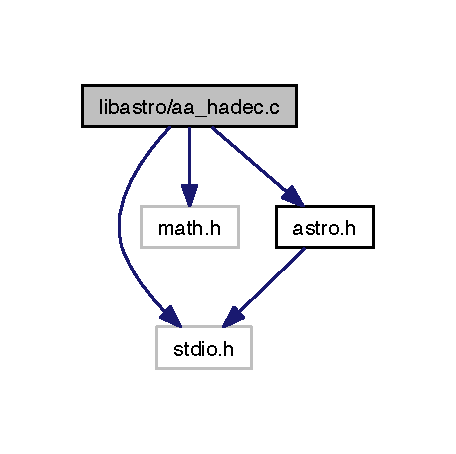
\includegraphics[width=219pt]{aa__hadec_8c__incl}
\end{center}
\end{figure}
\subsection*{Functions}
\begin{DoxyCompactItemize}
\item 
static void \hyperlink{aa__hadec_8c_a11564f6f3dea0f39fe5e59f3ee90b6aa}{aaha\-\_\-aux} (double lt, double x, double y, double $\ast$p, double $\ast$q)
\item 
void \hyperlink{aa__hadec_8c_afb4e9b19dfbf97eaf03b05111e9e919d}{aa\-\_\-hadec} (double lt, double alt, double az, double $\ast$ha, double $\ast$\hyperlink{constel_8c_a69b9a761071ef54b54c6970eb304268f}{dec})
\item 
void \hyperlink{aa__hadec_8c_a8ce2fb9152b3b6d728cda9ac4962378e}{hadec\-\_\-aa} (double lt, double ha, double \hyperlink{constel_8c_a69b9a761071ef54b54c6970eb304268f}{dec}, double $\ast$alt, double $\ast$az)
\end{DoxyCompactItemize}
\subsection*{Variables}
\begin{DoxyCompactItemize}
\item 
static char $\ast$ \hyperlink{aa__hadec_8c_ae037a79cb31f056d04153837887f5813}{rcsid} \mbox{[}2\mbox{]} = \{(char $\ast$)rcsid, \char`\"{}@(\#) \$R\-C\-Sfile\-: \hyperlink{circum_8c_aafc737ea9ef91f59cf9acd287fb8d085}{aa\-\_\-hadec.\-c},v \$ \$Date\-: 2003/03/20 08\-:51\-:37 \$ \$Revision\-: 1.\-3 \$ \$Name\-: \$\char`\"{}\}
\end{DoxyCompactItemize}


\subsection{Function Documentation}
\hypertarget{aa__hadec_8c_afb4e9b19dfbf97eaf03b05111e9e919d}{\index{aa\-\_\-hadec.\-c@{aa\-\_\-hadec.\-c}!aa\-\_\-hadec@{aa\-\_\-hadec}}
\index{aa\-\_\-hadec@{aa\-\_\-hadec}!aa_hadec.c@{aa\-\_\-hadec.\-c}}
\subsubsection[{aa\-\_\-hadec}]{\setlength{\rightskip}{0pt plus 5cm}void aa\-\_\-hadec (
\begin{DoxyParamCaption}
\item[{double}]{lt, }
\item[{double}]{alt, }
\item[{double}]{az, }
\item[{double $\ast$}]{ha, }
\item[{double $\ast$}]{dec}
\end{DoxyParamCaption}
)}}\label{aa__hadec_8c_afb4e9b19dfbf97eaf03b05111e9e919d}


Definition at line 16 of file aa\-\_\-hadec.\-c.



Here is the call graph for this function\-:
\nopagebreak
\begin{figure}[H]
\begin{center}
\leavevmode
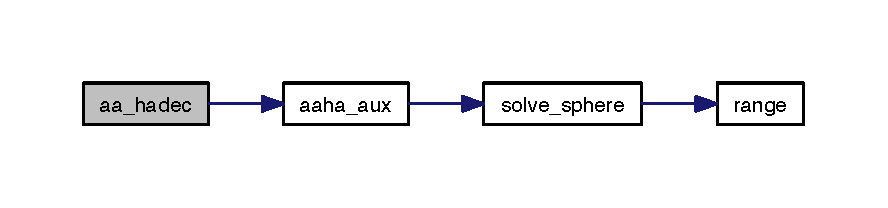
\includegraphics[width=350pt]{aa__hadec_8c_afb4e9b19dfbf97eaf03b05111e9e919d_cgraph}
\end{center}
\end{figure}




Here is the caller graph for this function\-:
\nopagebreak
\begin{figure}[H]
\begin{center}
\leavevmode
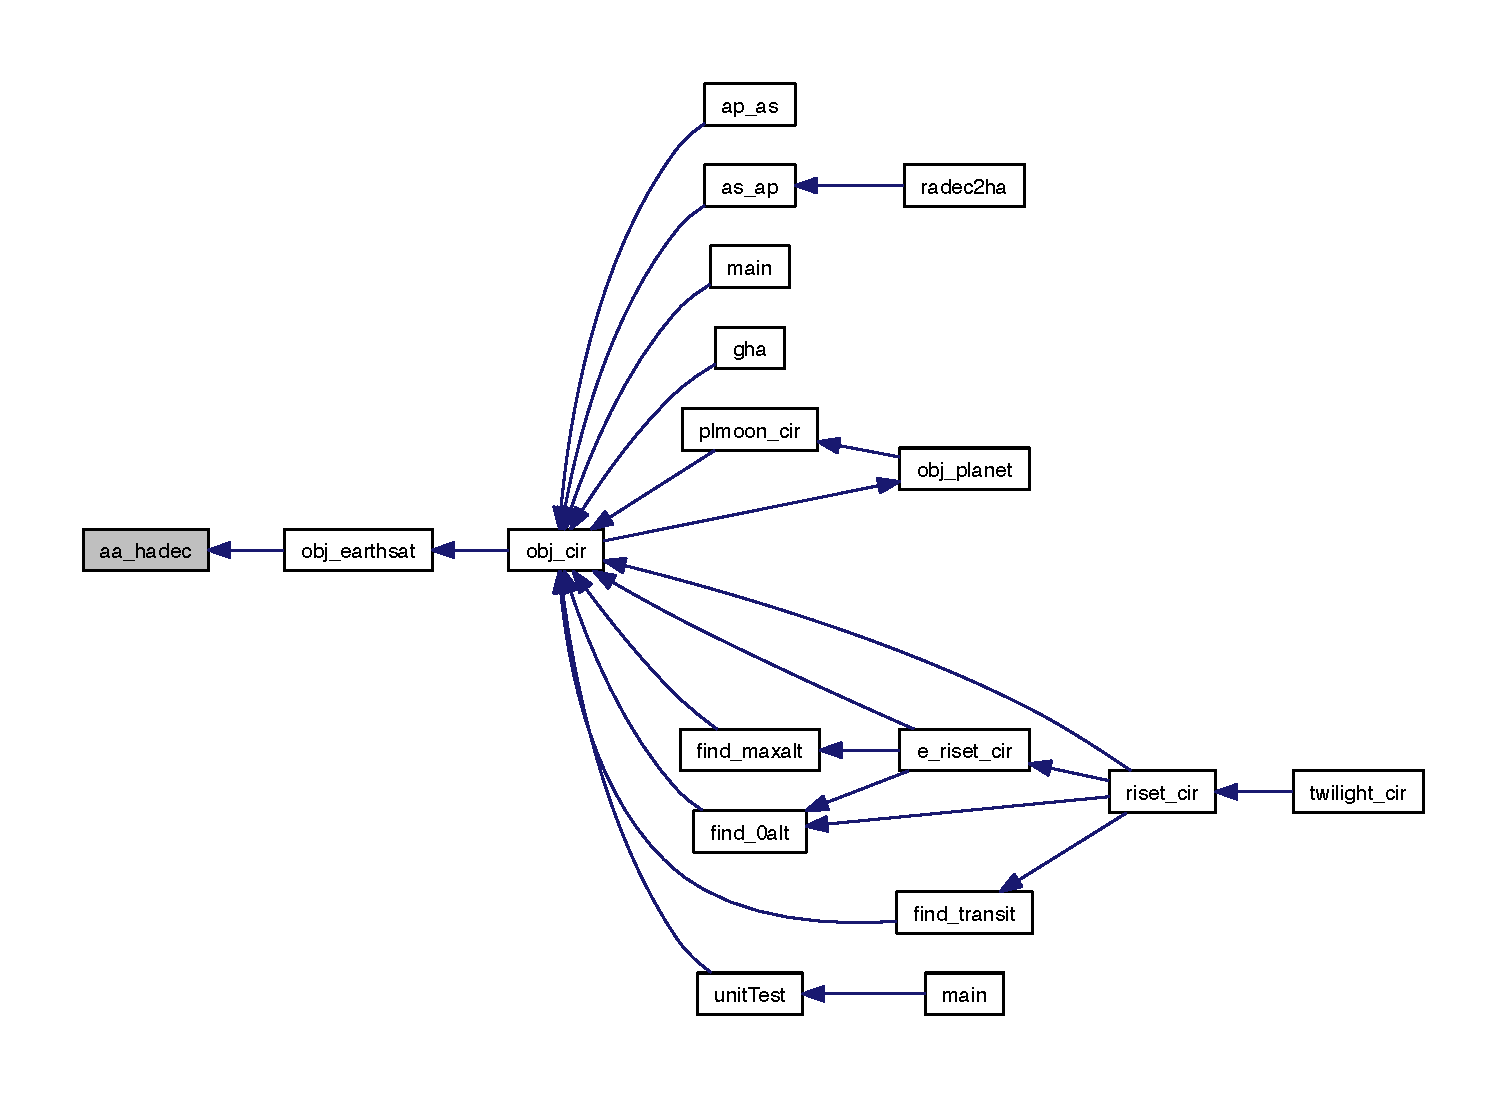
\includegraphics[width=350pt]{aa__hadec_8c_afb4e9b19dfbf97eaf03b05111e9e919d_icgraph}
\end{center}
\end{figure}


\hypertarget{aa__hadec_8c_a11564f6f3dea0f39fe5e59f3ee90b6aa}{\index{aa\-\_\-hadec.\-c@{aa\-\_\-hadec.\-c}!aaha\-\_\-aux@{aaha\-\_\-aux}}
\index{aaha\-\_\-aux@{aaha\-\_\-aux}!aa_hadec.c@{aa\-\_\-hadec.\-c}}
\subsubsection[{aaha\-\_\-aux}]{\setlength{\rightskip}{0pt plus 5cm}static void aaha\-\_\-aux (
\begin{DoxyParamCaption}
\item[{double}]{lt, }
\item[{double}]{x, }
\item[{double}]{y, }
\item[{double $\ast$}]{p, }
\item[{double $\ast$}]{q}
\end{DoxyParamCaption}
)\hspace{0.3cm}{\ttfamily [static]}}}\label{aa__hadec_8c_a11564f6f3dea0f39fe5e59f3ee90b6aa}


Definition at line 57 of file aa\-\_\-hadec.\-c.



Here is the call graph for this function\-:
\nopagebreak
\begin{figure}[H]
\begin{center}
\leavevmode
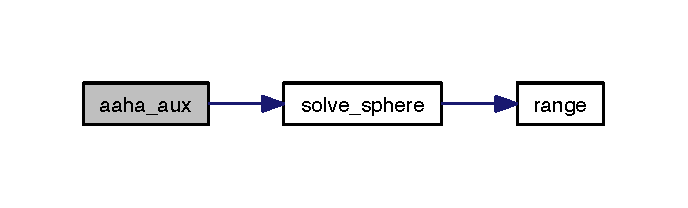
\includegraphics[width=330pt]{aa__hadec_8c_a11564f6f3dea0f39fe5e59f3ee90b6aa_cgraph}
\end{center}
\end{figure}




Here is the caller graph for this function\-:
\nopagebreak
\begin{figure}[H]
\begin{center}
\leavevmode
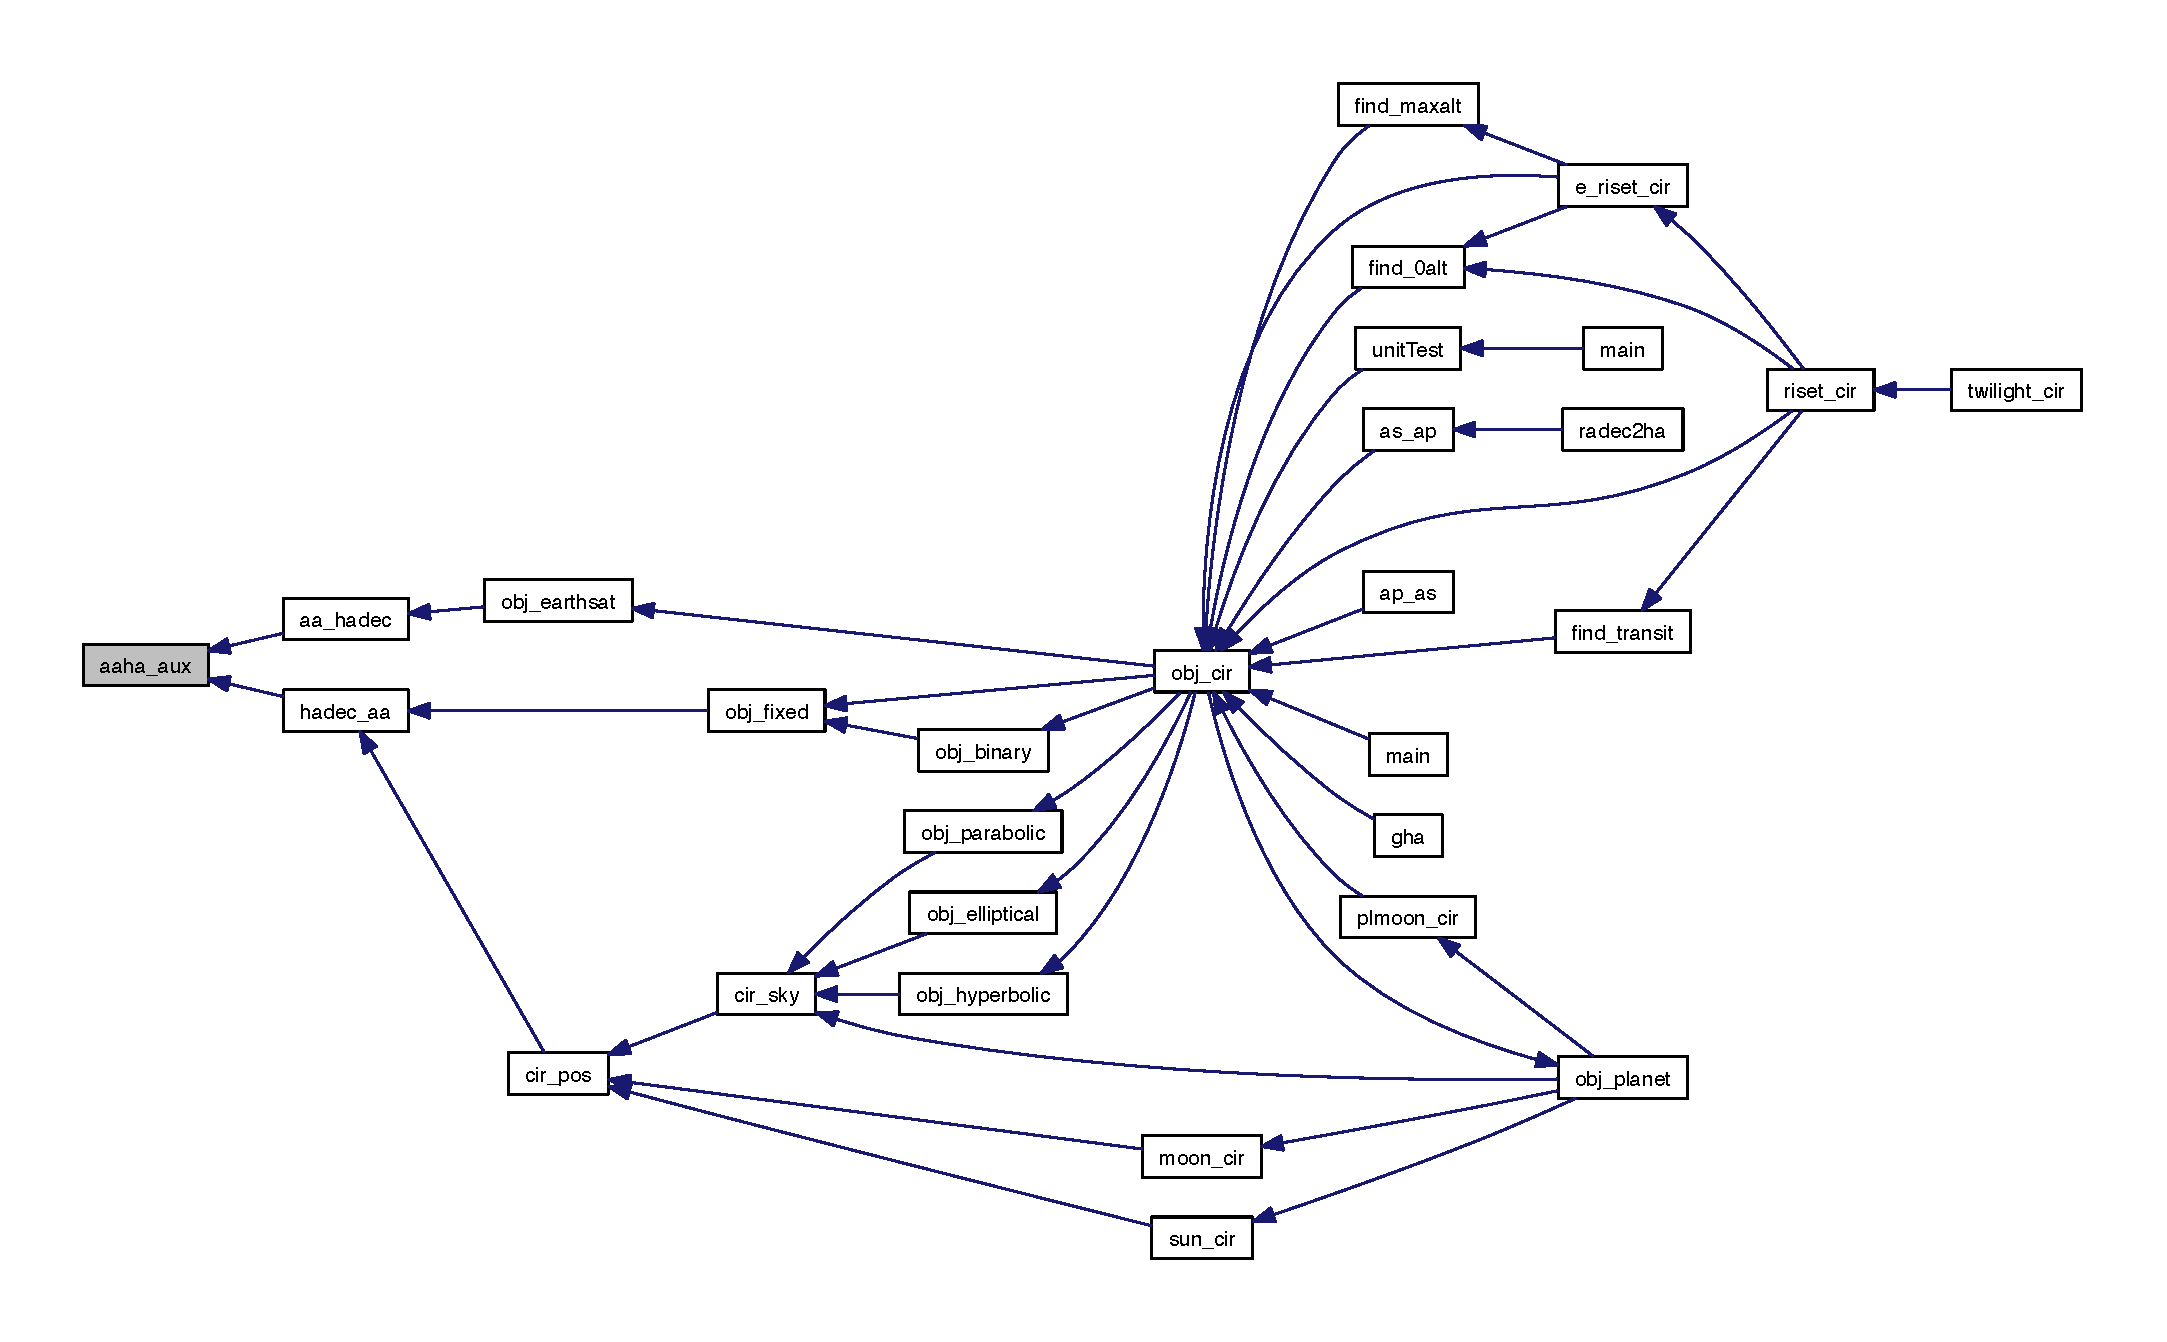
\includegraphics[width=350pt]{aa__hadec_8c_a11564f6f3dea0f39fe5e59f3ee90b6aa_icgraph}
\end{center}
\end{figure}


\hypertarget{aa__hadec_8c_a8ce2fb9152b3b6d728cda9ac4962378e}{\index{aa\-\_\-hadec.\-c@{aa\-\_\-hadec.\-c}!hadec\-\_\-aa@{hadec\-\_\-aa}}
\index{hadec\-\_\-aa@{hadec\-\_\-aa}!aa_hadec.c@{aa\-\_\-hadec.\-c}}
\subsubsection[{hadec\-\_\-aa}]{\setlength{\rightskip}{0pt plus 5cm}void hadec\-\_\-aa (
\begin{DoxyParamCaption}
\item[{double}]{lt, }
\item[{double}]{ha, }
\item[{double}]{dec, }
\item[{double $\ast$}]{alt, }
\item[{double $\ast$}]{az}
\end{DoxyParamCaption}
)}}\label{aa__hadec_8c_a8ce2fb9152b3b6d728cda9ac4962378e}


Definition at line 31 of file aa\-\_\-hadec.\-c.



Here is the call graph for this function\-:
\nopagebreak
\begin{figure}[H]
\begin{center}
\leavevmode
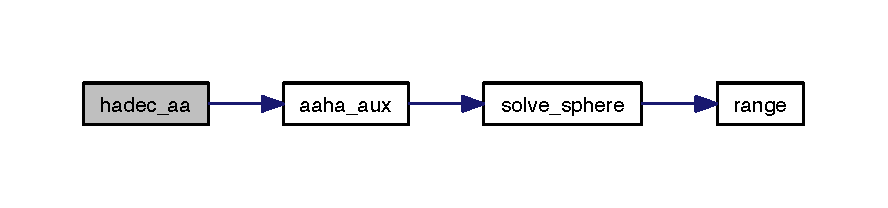
\includegraphics[width=350pt]{aa__hadec_8c_a8ce2fb9152b3b6d728cda9ac4962378e_cgraph}
\end{center}
\end{figure}




Here is the caller graph for this function\-:
\nopagebreak
\begin{figure}[H]
\begin{center}
\leavevmode
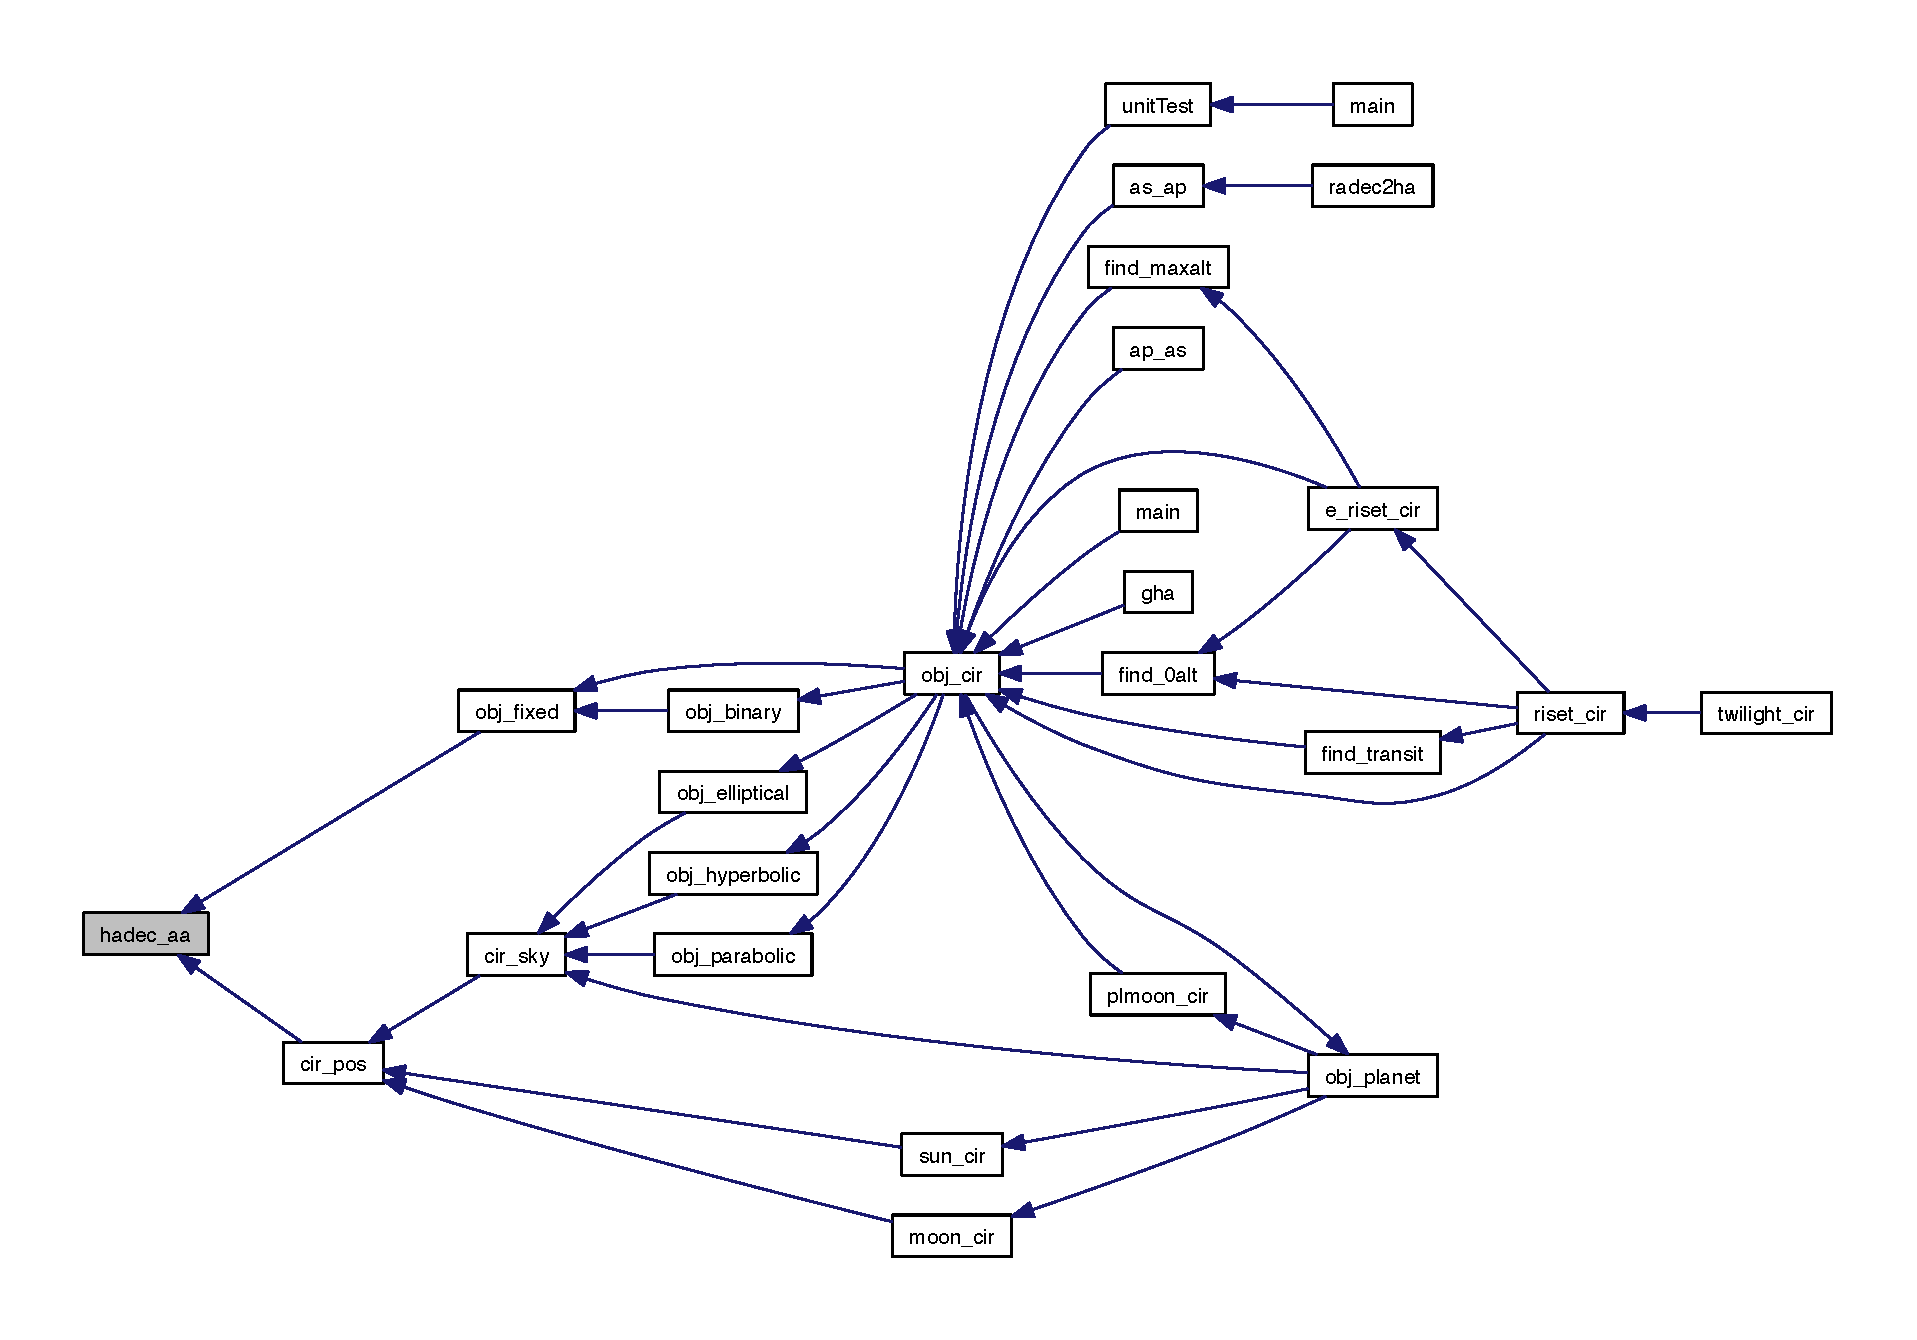
\includegraphics[width=350pt]{aa__hadec_8c_a8ce2fb9152b3b6d728cda9ac4962378e_icgraph}
\end{center}
\end{figure}




\subsection{Variable Documentation}
\hypertarget{aa__hadec_8c_ae037a79cb31f056d04153837887f5813}{\index{aa\-\_\-hadec.\-c@{aa\-\_\-hadec.\-c}!rcsid@{rcsid}}
\index{rcsid@{rcsid}!aa_hadec.c@{aa\-\_\-hadec.\-c}}
\subsubsection[{rcsid}]{\setlength{\rightskip}{0pt plus 5cm}char$\ast$ rcsid\mbox{[}2\mbox{]} = \{(char $\ast$)rcsid, \char`\"{}@(\#) \$R\-C\-Sfile\-: {\bf aa\-\_\-hadec.\-c},v \$ \$Date\-: 2003/03/20 08\-:51\-:37 \$ \$Revision\-: 1.\-3 \$ \$Name\-: \$\char`\"{}\}\hspace{0.3cm}{\ttfamily [static]}}}\label{aa__hadec_8c_ae037a79cb31f056d04153837887f5813}


Definition at line 77 of file aa\-\_\-hadec.\-c.


\hypertarget{aberration_8c}{\section{libastro/aberration.c File Reference}
\label{aberration_8c}\index{libastro/aberration.\-c@{libastro/aberration.\-c}}
}
{\ttfamily \#include $<$stdio.\-h$>$}\\*
{\ttfamily \#include $<$math.\-h$>$}\\*
{\ttfamily \#include $<$stdlib.\-h$>$}\\*
{\ttfamily \#include \char`\"{}astro.\-h\char`\"{}}\\*
Include dependency graph for aberration.\-c\-:
\nopagebreak
\begin{figure}[H]
\begin{center}
\leavevmode
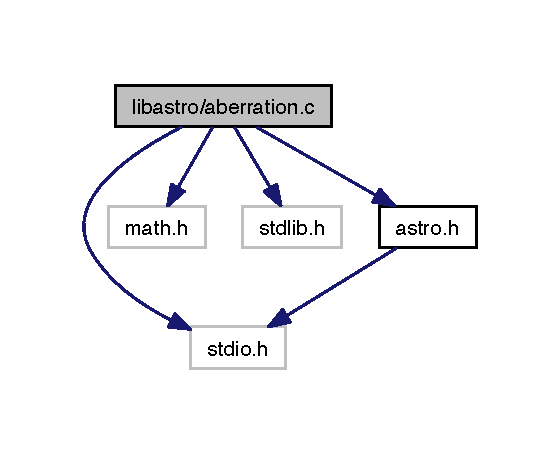
\includegraphics[width=268pt]{aberration_8c__incl}
\end{center}
\end{figure}
\subsection*{Macros}
\begin{DoxyCompactItemize}
\item 
\#define \hyperlink{aberration_8c_a611277b15b655248eab0728261ebcab2}{A\-B\-E\-R\-R\-\_\-\-C\-O\-N\-S\-T}~(20.\-49552/3600./180.$\ast$\hyperlink{twobody_8c_a598a3330b3c21701223ee0ca14316eca}{P\-I})  /$\ast$ aberr const in rad $\ast$/
\item 
\#define \hyperlink{aberration_8c_a382cb1176f2f63a3a7d590e0d4f276e3}{A\-B\-\_\-\-E\-C\-L\-\_\-\-E\-O\-D}~0
\item 
\#define \hyperlink{aberration_8c_ac504414c7ed784d95dcff73337dd3ead}{A\-B\-\_\-\-E\-Q\-\_\-\-E\-O\-D}~1
\end{DoxyCompactItemize}
\subsection*{Functions}
\begin{DoxyCompactItemize}
\item 
static void \hyperlink{aberration_8c_aa11d6eb5cd66a91726a712ee4c6da790}{ab\-\_\-aux} (double mj, double $\ast$x, double $\ast$y, double lsn, int mode)
\item 
void \hyperlink{aberration_8c_ae7956416613e0710a66903afc8d58639}{ab\-\_\-ecl} (double mj, double lsn, double $\ast$lam, double $\ast$bet)
\item 
void \hyperlink{aberration_8c_a0a01774c4e097c9ef5e17054c4509fc0}{ab\-\_\-eq} (double mj, double lsn, double $\ast$\hyperlink{constel_8c_aeb704957d1ce8d0299718c60f3cd3a4c}{ra}, double $\ast$\hyperlink{constel_8c_a69b9a761071ef54b54c6970eb304268f}{dec})
\end{DoxyCompactItemize}
\subsection*{Variables}
\begin{DoxyCompactItemize}
\item 
static char $\ast$ \hyperlink{aberration_8c_ae037a79cb31f056d04153837887f5813}{rcsid} \mbox{[}2\mbox{]} = \{(char $\ast$)rcsid, \char`\"{}@(\#) \$R\-C\-Sfile\-: \hyperlink{circum_8c_aafc737ea9ef91f59cf9acd287fb8d085}{aberration.\-c},v \$ \$Date\-: 2006/08/28 00\-:22\-:26 \$ \$Revision\-: 1.\-6 \$ \$Name\-: \$\char`\"{}\}
\end{DoxyCompactItemize}


\subsection{Macro Definition Documentation}
\hypertarget{aberration_8c_a382cb1176f2f63a3a7d590e0d4f276e3}{\index{aberration.\-c@{aberration.\-c}!A\-B\-\_\-\-E\-C\-L\-\_\-\-E\-O\-D@{A\-B\-\_\-\-E\-C\-L\-\_\-\-E\-O\-D}}
\index{A\-B\-\_\-\-E\-C\-L\-\_\-\-E\-O\-D@{A\-B\-\_\-\-E\-C\-L\-\_\-\-E\-O\-D}!aberration.c@{aberration.\-c}}
\subsubsection[{A\-B\-\_\-\-E\-C\-L\-\_\-\-E\-O\-D}]{\setlength{\rightskip}{0pt plus 5cm}\#define A\-B\-\_\-\-E\-C\-L\-\_\-\-E\-O\-D~0}}\label{aberration_8c_a382cb1176f2f63a3a7d590e0d4f276e3}


Definition at line 15 of file aberration.\-c.

\hypertarget{aberration_8c_ac504414c7ed784d95dcff73337dd3ead}{\index{aberration.\-c@{aberration.\-c}!A\-B\-\_\-\-E\-Q\-\_\-\-E\-O\-D@{A\-B\-\_\-\-E\-Q\-\_\-\-E\-O\-D}}
\index{A\-B\-\_\-\-E\-Q\-\_\-\-E\-O\-D@{A\-B\-\_\-\-E\-Q\-\_\-\-E\-O\-D}!aberration.c@{aberration.\-c}}
\subsubsection[{A\-B\-\_\-\-E\-Q\-\_\-\-E\-O\-D}]{\setlength{\rightskip}{0pt plus 5cm}\#define A\-B\-\_\-\-E\-Q\-\_\-\-E\-O\-D~1}}\label{aberration_8c_ac504414c7ed784d95dcff73337dd3ead}


Definition at line 16 of file aberration.\-c.

\hypertarget{aberration_8c_a611277b15b655248eab0728261ebcab2}{\index{aberration.\-c@{aberration.\-c}!A\-B\-E\-R\-R\-\_\-\-C\-O\-N\-S\-T@{A\-B\-E\-R\-R\-\_\-\-C\-O\-N\-S\-T}}
\index{A\-B\-E\-R\-R\-\_\-\-C\-O\-N\-S\-T@{A\-B\-E\-R\-R\-\_\-\-C\-O\-N\-S\-T}!aberration.c@{aberration.\-c}}
\subsubsection[{A\-B\-E\-R\-R\-\_\-\-C\-O\-N\-S\-T}]{\setlength{\rightskip}{0pt plus 5cm}\#define A\-B\-E\-R\-R\-\_\-\-C\-O\-N\-S\-T~(20.\-49552/3600./180.$\ast${\bf P\-I})  /$\ast$ aberr const in rad $\ast$/}}\label{aberration_8c_a611277b15b655248eab0728261ebcab2}


Definition at line 14 of file aberration.\-c.



\subsection{Function Documentation}
\hypertarget{aberration_8c_aa11d6eb5cd66a91726a712ee4c6da790}{\index{aberration.\-c@{aberration.\-c}!ab\-\_\-aux@{ab\-\_\-aux}}
\index{ab\-\_\-aux@{ab\-\_\-aux}!aberration.c@{aberration.\-c}}
\subsubsection[{ab\-\_\-aux}]{\setlength{\rightskip}{0pt plus 5cm}static void ab\-\_\-aux (
\begin{DoxyParamCaption}
\item[{double}]{mj, }
\item[{double $\ast$}]{x, }
\item[{double $\ast$}]{y, }
\item[{double}]{lsn, }
\item[{int}]{mode}
\end{DoxyParamCaption}
)\hspace{0.3cm}{\ttfamily [static]}}}\label{aberration_8c_aa11d6eb5cd66a91726a712ee4c6da790}


Definition at line 80 of file aberration.\-c.



Here is the call graph for this function\-:
\nopagebreak
\begin{figure}[H]
\begin{center}
\leavevmode
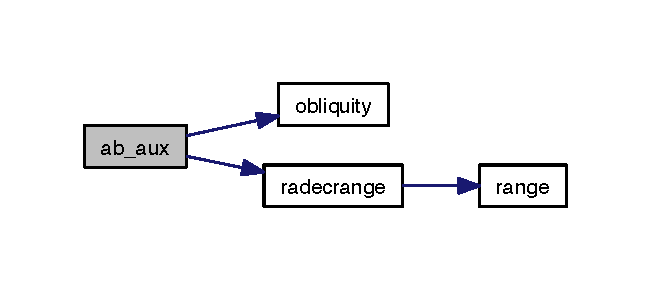
\includegraphics[width=312pt]{aberration_8c_aa11d6eb5cd66a91726a712ee4c6da790_cgraph}
\end{center}
\end{figure}




Here is the caller graph for this function\-:
\nopagebreak
\begin{figure}[H]
\begin{center}
\leavevmode
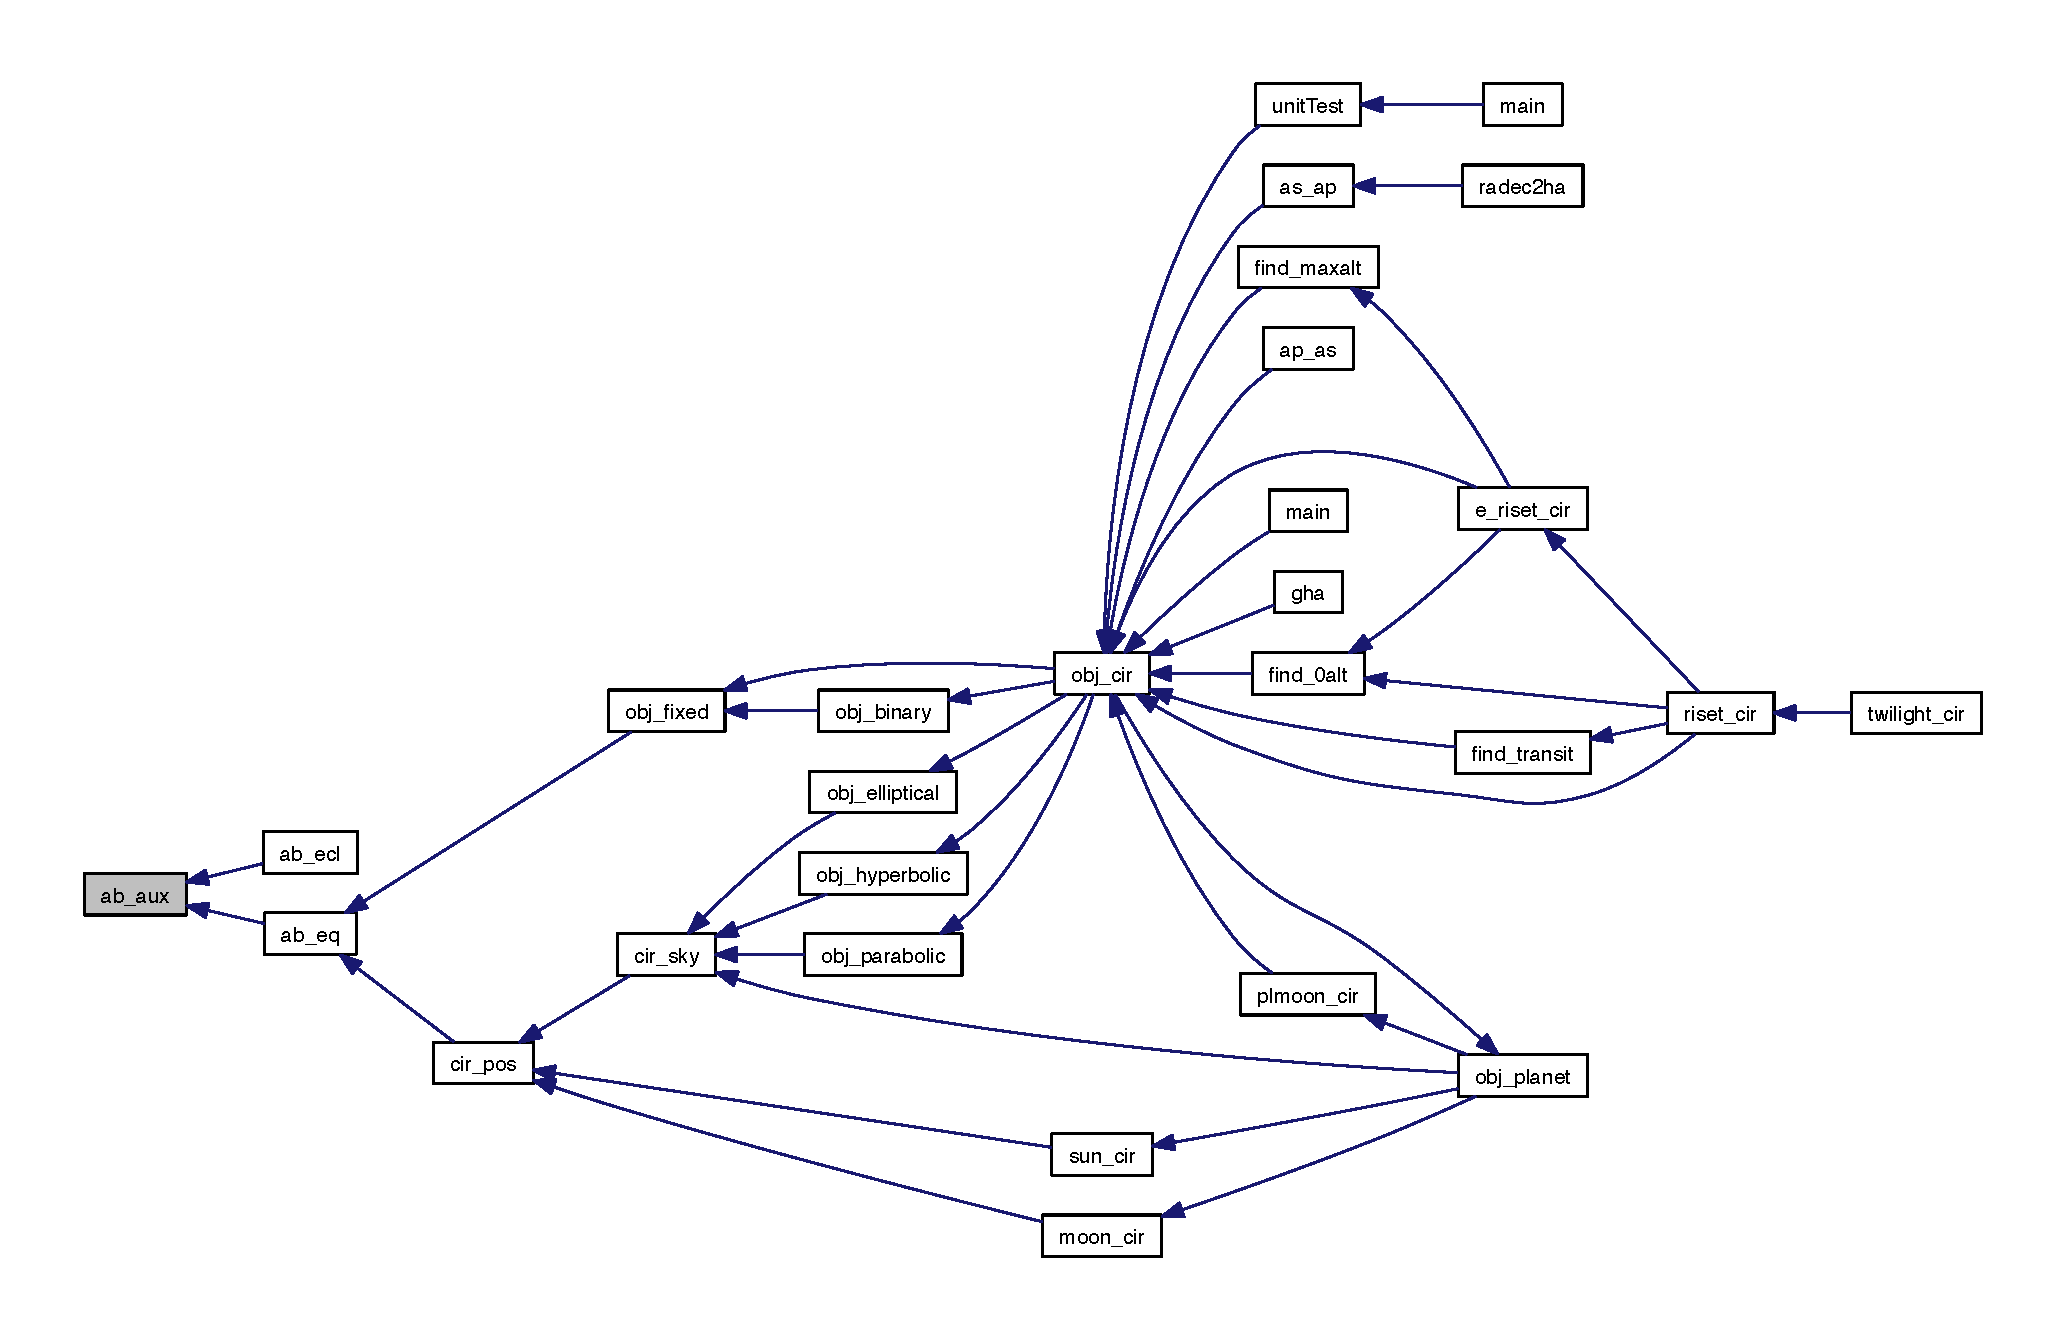
\includegraphics[width=350pt]{aberration_8c_aa11d6eb5cd66a91726a712ee4c6da790_icgraph}
\end{center}
\end{figure}


\hypertarget{aberration_8c_ae7956416613e0710a66903afc8d58639}{\index{aberration.\-c@{aberration.\-c}!ab\-\_\-ecl@{ab\-\_\-ecl}}
\index{ab\-\_\-ecl@{ab\-\_\-ecl}!aberration.c@{aberration.\-c}}
\subsubsection[{ab\-\_\-ecl}]{\setlength{\rightskip}{0pt plus 5cm}void ab\-\_\-ecl (
\begin{DoxyParamCaption}
\item[{double}]{mj, }
\item[{double}]{lsn, }
\item[{double $\ast$}]{lam, }
\item[{double $\ast$}]{bet}
\end{DoxyParamCaption}
)}}\label{aberration_8c_ae7956416613e0710a66903afc8d58639}


Definition at line 25 of file aberration.\-c.



Here is the call graph for this function\-:
\nopagebreak
\begin{figure}[H]
\begin{center}
\leavevmode
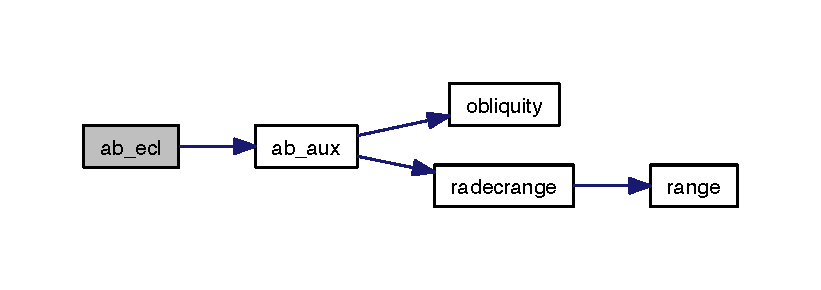
\includegraphics[width=350pt]{aberration_8c_ae7956416613e0710a66903afc8d58639_cgraph}
\end{center}
\end{figure}


\hypertarget{aberration_8c_a0a01774c4e097c9ef5e17054c4509fc0}{\index{aberration.\-c@{aberration.\-c}!ab\-\_\-eq@{ab\-\_\-eq}}
\index{ab\-\_\-eq@{ab\-\_\-eq}!aberration.c@{aberration.\-c}}
\subsubsection[{ab\-\_\-eq}]{\setlength{\rightskip}{0pt plus 5cm}void ab\-\_\-eq (
\begin{DoxyParamCaption}
\item[{double}]{mj, }
\item[{double}]{lsn, }
\item[{double $\ast$}]{ra, }
\item[{double $\ast$}]{dec}
\end{DoxyParamCaption}
)}}\label{aberration_8c_a0a01774c4e097c9ef5e17054c4509fc0}


Definition at line 35 of file aberration.\-c.



Here is the call graph for this function\-:
\nopagebreak
\begin{figure}[H]
\begin{center}
\leavevmode
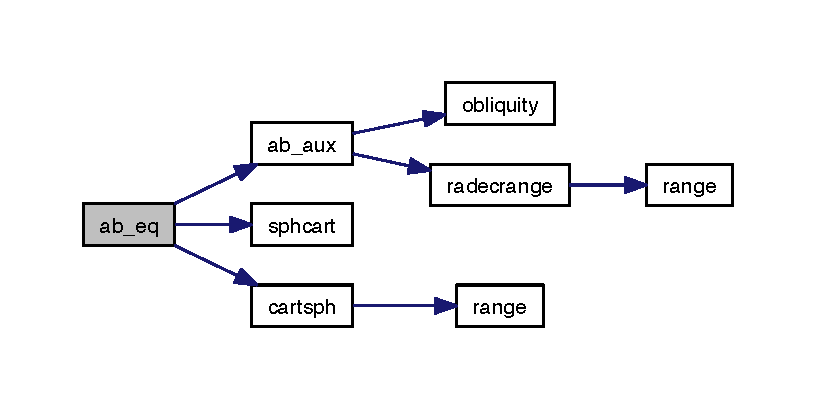
\includegraphics[width=350pt]{aberration_8c_a0a01774c4e097c9ef5e17054c4509fc0_cgraph}
\end{center}
\end{figure}




Here is the caller graph for this function\-:
\nopagebreak
\begin{figure}[H]
\begin{center}
\leavevmode
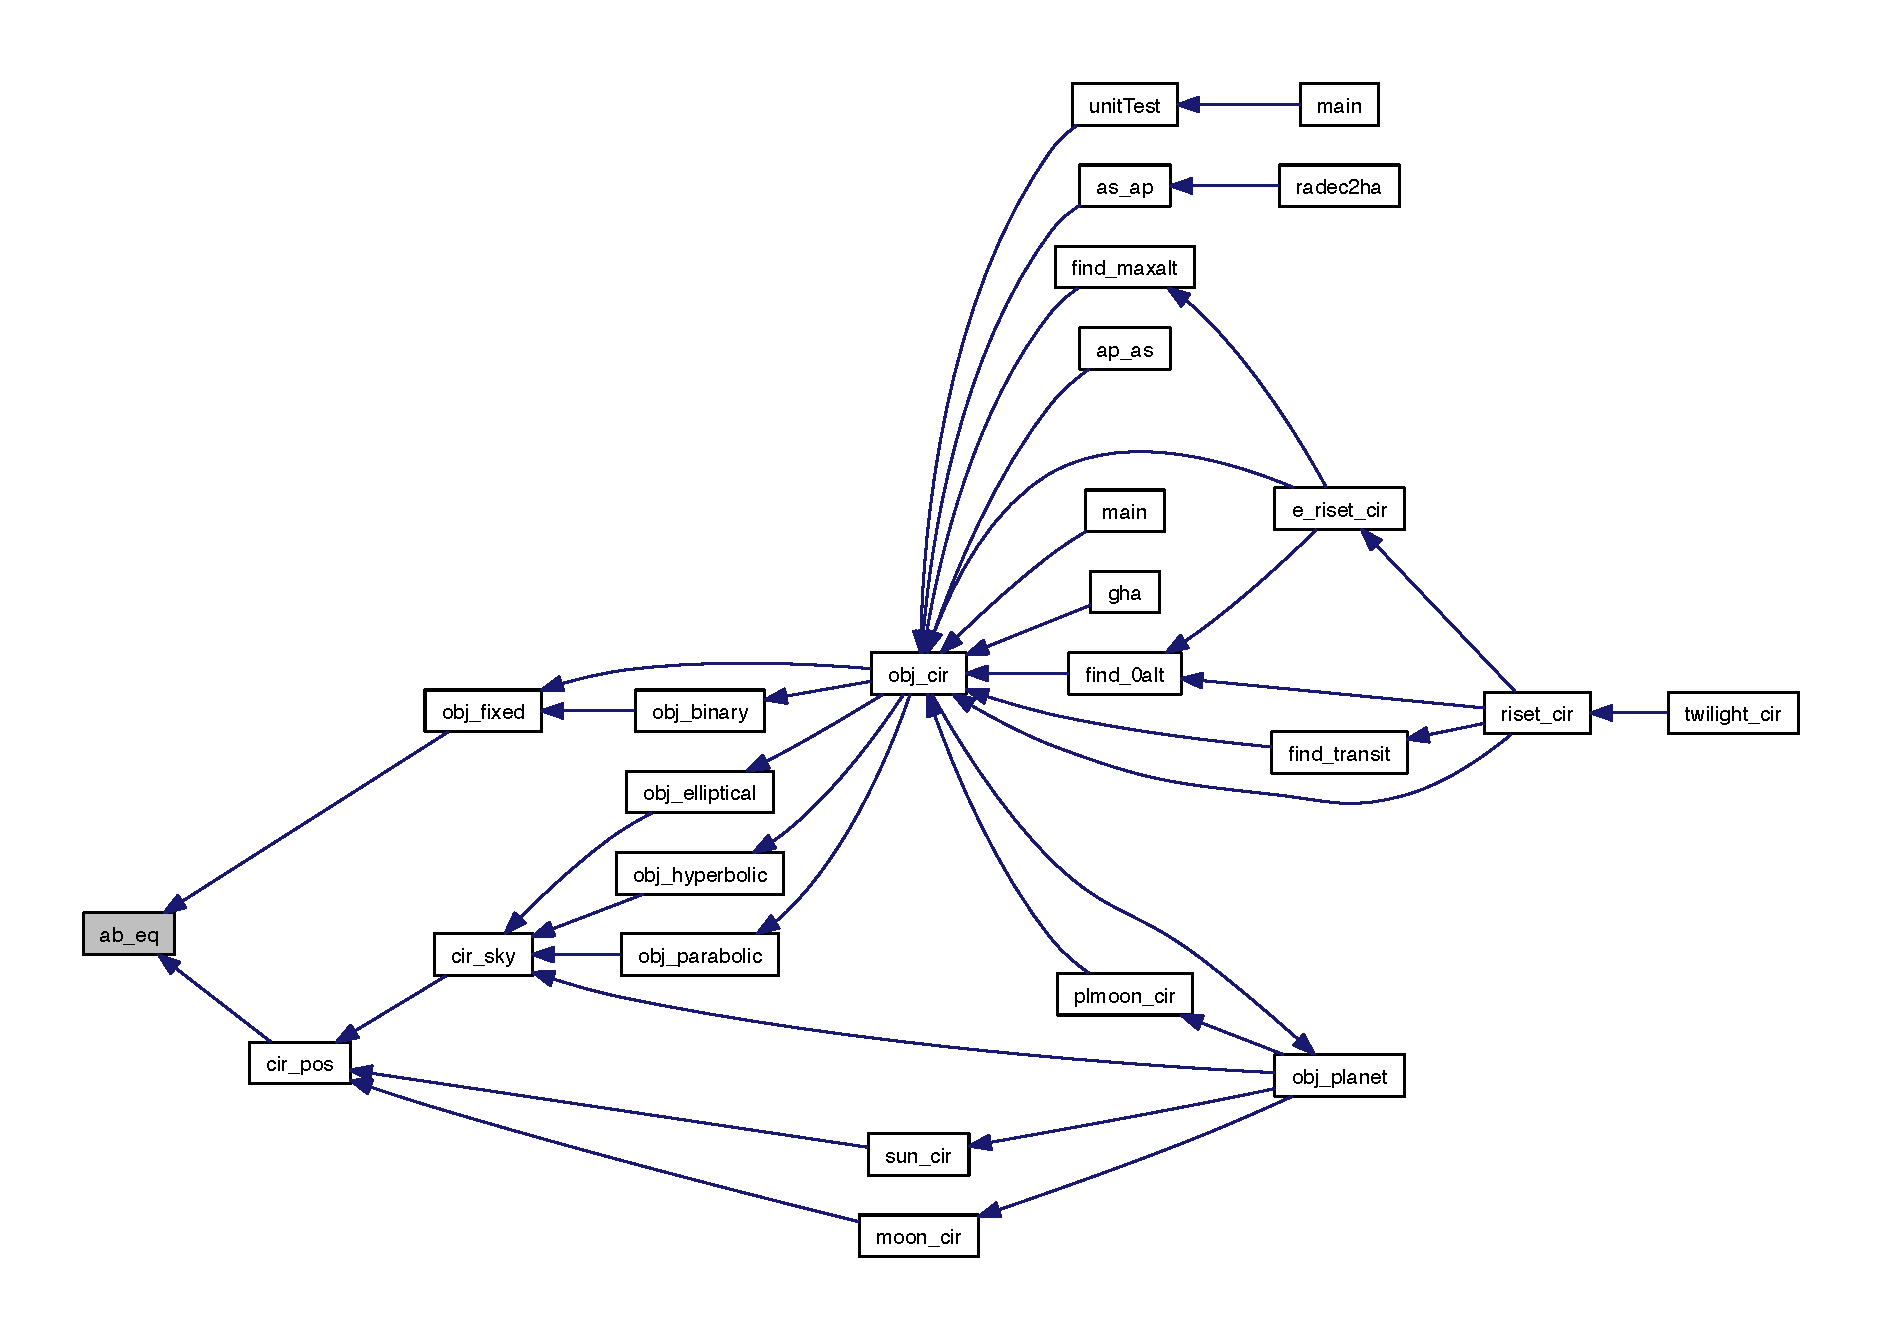
\includegraphics[width=350pt]{aberration_8c_a0a01774c4e097c9ef5e17054c4509fc0_icgraph}
\end{center}
\end{figure}




\subsection{Variable Documentation}
\hypertarget{aberration_8c_ae037a79cb31f056d04153837887f5813}{\index{aberration.\-c@{aberration.\-c}!rcsid@{rcsid}}
\index{rcsid@{rcsid}!aberration.c@{aberration.\-c}}
\subsubsection[{rcsid}]{\setlength{\rightskip}{0pt plus 5cm}char$\ast$ rcsid\mbox{[}2\mbox{]} = \{(char $\ast$)rcsid, \char`\"{}@(\#) \$R\-C\-Sfile\-: {\bf aberration.\-c},v \$ \$Date\-: 2006/08/28 00\-:22\-:26 \$ \$Revision\-: 1.\-6 \$ \$Name\-: \$\char`\"{}\}\hspace{0.3cm}{\ttfamily [static]}}}\label{aberration_8c_ae037a79cb31f056d04153837887f5813}


Definition at line 161 of file aberration.\-c.


\hypertarget{actan_8c}{\section{libastro/actan.c File Reference}
\label{actan_8c}\index{libastro/actan.\-c@{libastro/actan.\-c}}
}
{\ttfamily \#include $<$math.\-h$>$}\\*
Include dependency graph for actan.\-c\-:
\nopagebreak
\begin{figure}[H]
\begin{center}
\leavevmode
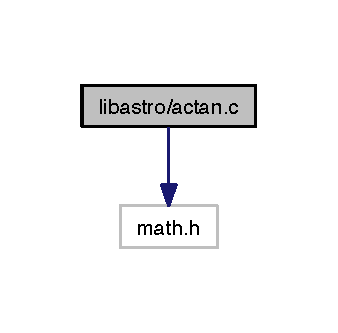
\includegraphics[width=162pt]{actan_8c__incl}
\end{center}
\end{figure}
\subsection*{Macros}
\begin{DoxyCompactItemize}
\item 
\#define \hyperlink{actan_8c_ae71449b1cc6e6250b91f539153a7a0d3}{M\-\_\-\-P\-I}~3.\-14159265358979323846
\item 
\#define \hyperlink{actan_8c_a958e4508ed28ee5cc04249144312c15f}{M\-\_\-\-P\-I\-\_\-2}~1.\-57079632679489661923
\end{DoxyCompactItemize}
\subsection*{Functions}
\begin{DoxyCompactItemize}
\item 
double \hyperlink{actan_8c_a8f64856d35ec46cef389467fb299d35e}{actan} (double sinx, double cosx)
\end{DoxyCompactItemize}
\subsection*{Variables}
\begin{DoxyCompactItemize}
\item 
static char $\ast$ \hyperlink{actan_8c_ae037a79cb31f056d04153837887f5813}{rcsid} \mbox{[}2\mbox{]} = \{(char $\ast$)rcsid, \char`\"{}@(\#) \$R\-C\-Sfile\-: \hyperlink{circum_8c_aafc737ea9ef91f59cf9acd287fb8d085}{actan.\-c},v \$ \$Date\-: 2001/01/10 16\-:32\-:21 \$ \$Revision\-: 1.\-3 \$ \$Name\-: \$\char`\"{}\}
\end{DoxyCompactItemize}


\subsection{Macro Definition Documentation}
\hypertarget{actan_8c_ae71449b1cc6e6250b91f539153a7a0d3}{\index{actan.\-c@{actan.\-c}!M\-\_\-\-P\-I@{M\-\_\-\-P\-I}}
\index{M\-\_\-\-P\-I@{M\-\_\-\-P\-I}!actan.c@{actan.\-c}}
\subsubsection[{M\-\_\-\-P\-I}]{\setlength{\rightskip}{0pt plus 5cm}\#define M\-\_\-\-P\-I~3.\-14159265358979323846}}\label{actan_8c_ae71449b1cc6e6250b91f539153a7a0d3}


Definition at line 7 of file actan.\-c.

\hypertarget{actan_8c_a958e4508ed28ee5cc04249144312c15f}{\index{actan.\-c@{actan.\-c}!M\-\_\-\-P\-I\-\_\-2@{M\-\_\-\-P\-I\-\_\-2}}
\index{M\-\_\-\-P\-I\-\_\-2@{M\-\_\-\-P\-I\-\_\-2}!actan.c@{actan.\-c}}
\subsubsection[{M\-\_\-\-P\-I\-\_\-2}]{\setlength{\rightskip}{0pt plus 5cm}\#define M\-\_\-\-P\-I\-\_\-2~1.\-57079632679489661923}}\label{actan_8c_a958e4508ed28ee5cc04249144312c15f}


Definition at line 8 of file actan.\-c.



\subsection{Function Documentation}
\hypertarget{actan_8c_a8f64856d35ec46cef389467fb299d35e}{\index{actan.\-c@{actan.\-c}!actan@{actan}}
\index{actan@{actan}!actan.c@{actan.\-c}}
\subsubsection[{actan}]{\setlength{\rightskip}{0pt plus 5cm}double actan (
\begin{DoxyParamCaption}
\item[{double}]{sinx, }
\item[{double}]{cosx}
\end{DoxyParamCaption}
)}}\label{actan_8c_a8f64856d35ec46cef389467fb299d35e}


Definition at line 12 of file actan.\-c.



Here is the caller graph for this function\-:
\nopagebreak
\begin{figure}[H]
\begin{center}
\leavevmode
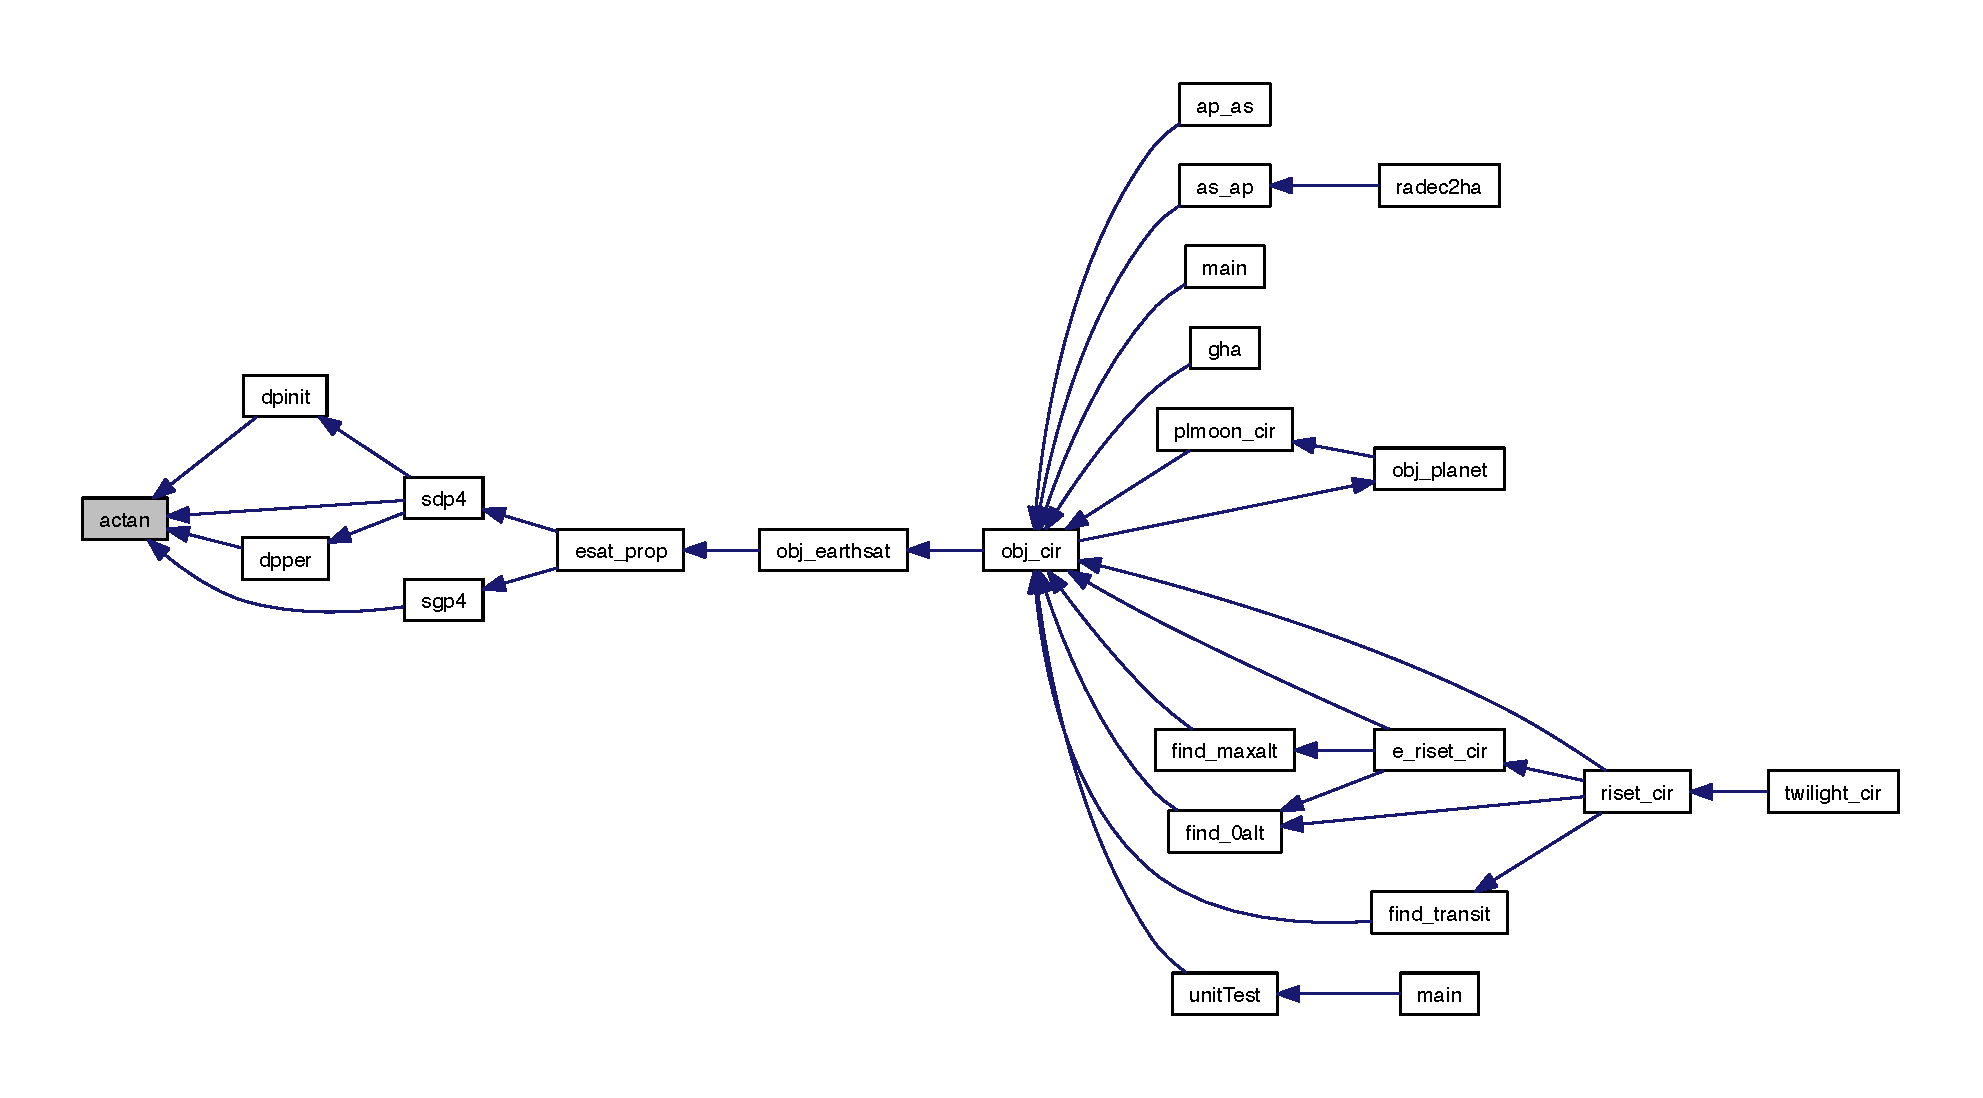
\includegraphics[width=350pt]{actan_8c_a8f64856d35ec46cef389467fb299d35e_icgraph}
\end{center}
\end{figure}




\subsection{Variable Documentation}
\hypertarget{actan_8c_ae037a79cb31f056d04153837887f5813}{\index{actan.\-c@{actan.\-c}!rcsid@{rcsid}}
\index{rcsid@{rcsid}!actan.c@{actan.\-c}}
\subsubsection[{rcsid}]{\setlength{\rightskip}{0pt plus 5cm}char$\ast$ rcsid\mbox{[}2\mbox{]} = \{(char $\ast$)rcsid, \char`\"{}@(\#) \$R\-C\-Sfile\-: {\bf actan.\-c},v \$ \$Date\-: 2001/01/10 16\-:32\-:21 \$ \$Revision\-: 1.\-3 \$ \$Name\-: \$\char`\"{}\}\hspace{0.3cm}{\ttfamily [static]}}}\label{actan_8c_ae037a79cb31f056d04153837887f5813}


Definition at line 67 of file actan.\-c.


\hypertarget{airmass_8c}{\section{libastro/airmass.c File Reference}
\label{airmass_8c}\index{libastro/airmass.\-c@{libastro/airmass.\-c}}
}
{\ttfamily \#include $<$math.\-h$>$}\\*
{\ttfamily \#include \char`\"{}astro.\-h\char`\"{}}\\*
Include dependency graph for airmass.\-c\-:
\nopagebreak
\begin{figure}[H]
\begin{center}
\leavevmode
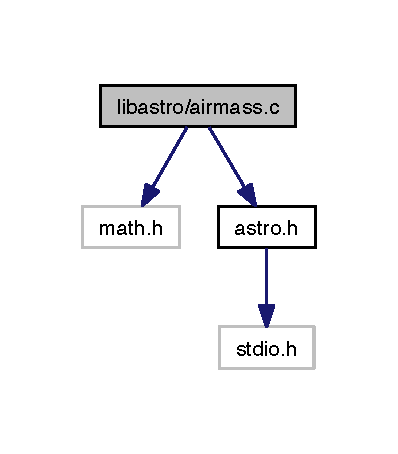
\includegraphics[width=191pt]{airmass_8c__incl}
\end{center}
\end{figure}
\subsection*{Functions}
\begin{DoxyCompactItemize}
\item 
void \hyperlink{airmass_8c_a0149c681dca5872a5194adc30048833e}{airmass} (double aa, double $\ast$Xp)
\end{DoxyCompactItemize}
\subsection*{Variables}
\begin{DoxyCompactItemize}
\item 
static char $\ast$ \hyperlink{airmass_8c_ae037a79cb31f056d04153837887f5813}{rcsid} \mbox{[}2\mbox{]} = \{(char $\ast$)rcsid, \char`\"{}@(\#) \$R\-C\-Sfile\-: \hyperlink{circum_8c_aafc737ea9ef91f59cf9acd287fb8d085}{airmass.\-c},v \$ \$Date\-: 2003/03/20 08\-:51\-:37 \$ \$Revision\-: 1.\-3 \$ \$Name\-: \$\char`\"{}\}
\end{DoxyCompactItemize}


\subsection{Function Documentation}
\hypertarget{airmass_8c_a0149c681dca5872a5194adc30048833e}{\index{airmass.\-c@{airmass.\-c}!airmass@{airmass}}
\index{airmass@{airmass}!airmass.c@{airmass.\-c}}
\subsubsection[{airmass}]{\setlength{\rightskip}{0pt plus 5cm}void airmass (
\begin{DoxyParamCaption}
\item[{double}]{aa, }
\item[{double $\ast$}]{Xp}
\end{DoxyParamCaption}
)}}\label{airmass_8c_a0149c681dca5872a5194adc30048833e}


Definition at line 11 of file airmass.\-c.



\subsection{Variable Documentation}
\hypertarget{airmass_8c_ae037a79cb31f056d04153837887f5813}{\index{airmass.\-c@{airmass.\-c}!rcsid@{rcsid}}
\index{rcsid@{rcsid}!airmass.c@{airmass.\-c}}
\subsubsection[{rcsid}]{\setlength{\rightskip}{0pt plus 5cm}char$\ast$ rcsid\mbox{[}2\mbox{]} = \{(char $\ast$)rcsid, \char`\"{}@(\#) \$R\-C\-Sfile\-: {\bf airmass.\-c},v \$ \$Date\-: 2003/03/20 08\-:51\-:37 \$ \$Revision\-: 1.\-3 \$ \$Name\-: \$\char`\"{}\}\hspace{0.3cm}{\ttfamily [static]}}}\label{airmass_8c_ae037a79cb31f056d04153837887f5813}


Definition at line 26 of file airmass.\-c.


\hypertarget{anomaly_8c}{\section{libastro/anomaly.c File Reference}
\label{anomaly_8c}\index{libastro/anomaly.\-c@{libastro/anomaly.\-c}}
}
{\ttfamily \#include $<$stdio.\-h$>$}\\*
{\ttfamily \#include $<$math.\-h$>$}\\*
{\ttfamily \#include \char`\"{}astro.\-h\char`\"{}}\\*
Include dependency graph for anomaly.\-c\-:
\nopagebreak
\begin{figure}[H]
\begin{center}
\leavevmode
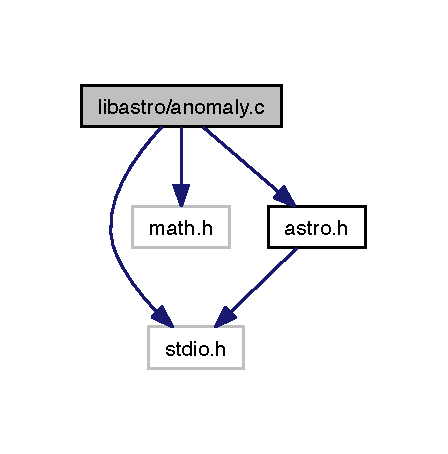
\includegraphics[width=215pt]{anomaly_8c__incl}
\end{center}
\end{figure}
\subsection*{Macros}
\begin{DoxyCompactItemize}
\item 
\#define \hyperlink{anomaly_8c_a4912c64aec0c943b7985db6cb61ff83a}{T\-W\-O\-P\-I}~(2$\ast$\hyperlink{twobody_8c_a598a3330b3c21701223ee0ca14316eca}{P\-I})
\item 
\#define \hyperlink{anomaly_8c_abc50633cd54df8c19edafaab298d8616}{S\-T\-O\-P\-E\-R\-R}~(1e-\/8)
\end{DoxyCompactItemize}
\subsection*{Functions}
\begin{DoxyCompactItemize}
\item 
void \hyperlink{anomaly_8c_ab35408588a03873bb6cfc73b8b7aa349}{anomaly} (double ma, double s, double $\ast$nu, double $\ast$ea)
\end{DoxyCompactItemize}
\subsection*{Variables}
\begin{DoxyCompactItemize}
\item 
static char $\ast$ \hyperlink{anomaly_8c_ae037a79cb31f056d04153837887f5813}{rcsid} \mbox{[}2\mbox{]} = \{(char $\ast$)rcsid, \char`\"{}@(\#) \$R\-C\-Sfile\-: \hyperlink{circum_8c_aafc737ea9ef91f59cf9acd287fb8d085}{anomaly.\-c},v \$ \$Date\-: 2003/03/20 08\-:51\-:37 \$ \$Revision\-: 1.\-3 \$ \$Name\-: \$\char`\"{}\}
\end{DoxyCompactItemize}


\subsection{Macro Definition Documentation}
\hypertarget{anomaly_8c_abc50633cd54df8c19edafaab298d8616}{\index{anomaly.\-c@{anomaly.\-c}!S\-T\-O\-P\-E\-R\-R@{S\-T\-O\-P\-E\-R\-R}}
\index{S\-T\-O\-P\-E\-R\-R@{S\-T\-O\-P\-E\-R\-R}!anomaly.c@{anomaly.\-c}}
\subsubsection[{S\-T\-O\-P\-E\-R\-R}]{\setlength{\rightskip}{0pt plus 5cm}\#define S\-T\-O\-P\-E\-R\-R~(1e-\/8)}}\label{anomaly_8c_abc50633cd54df8c19edafaab298d8616}


Definition at line 10 of file anomaly.\-c.

\hypertarget{anomaly_8c_a4912c64aec0c943b7985db6cb61ff83a}{\index{anomaly.\-c@{anomaly.\-c}!T\-W\-O\-P\-I@{T\-W\-O\-P\-I}}
\index{T\-W\-O\-P\-I@{T\-W\-O\-P\-I}!anomaly.c@{anomaly.\-c}}
\subsubsection[{T\-W\-O\-P\-I}]{\setlength{\rightskip}{0pt plus 5cm}\#define T\-W\-O\-P\-I~(2$\ast${\bf P\-I})}}\label{anomaly_8c_a4912c64aec0c943b7985db6cb61ff83a}


Definition at line 9 of file anomaly.\-c.



\subsection{Function Documentation}
\hypertarget{anomaly_8c_ab35408588a03873bb6cfc73b8b7aa349}{\index{anomaly.\-c@{anomaly.\-c}!anomaly@{anomaly}}
\index{anomaly@{anomaly}!anomaly.c@{anomaly.\-c}}
\subsubsection[{anomaly}]{\setlength{\rightskip}{0pt plus 5cm}void anomaly (
\begin{DoxyParamCaption}
\item[{double}]{ma, }
\item[{double}]{s, }
\item[{double $\ast$}]{nu, }
\item[{double $\ast$}]{ea}
\end{DoxyParamCaption}
)}}\label{anomaly_8c_ab35408588a03873bb6cfc73b8b7aa349}


Definition at line 17 of file anomaly.\-c.



Here is the call graph for this function\-:
\nopagebreak
\begin{figure}[H]
\begin{center}
\leavevmode
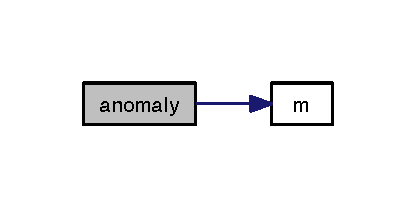
\includegraphics[width=200pt]{anomaly_8c_ab35408588a03873bb6cfc73b8b7aa349_cgraph}
\end{center}
\end{figure}




Here is the caller graph for this function\-:
\nopagebreak
\begin{figure}[H]
\begin{center}
\leavevmode
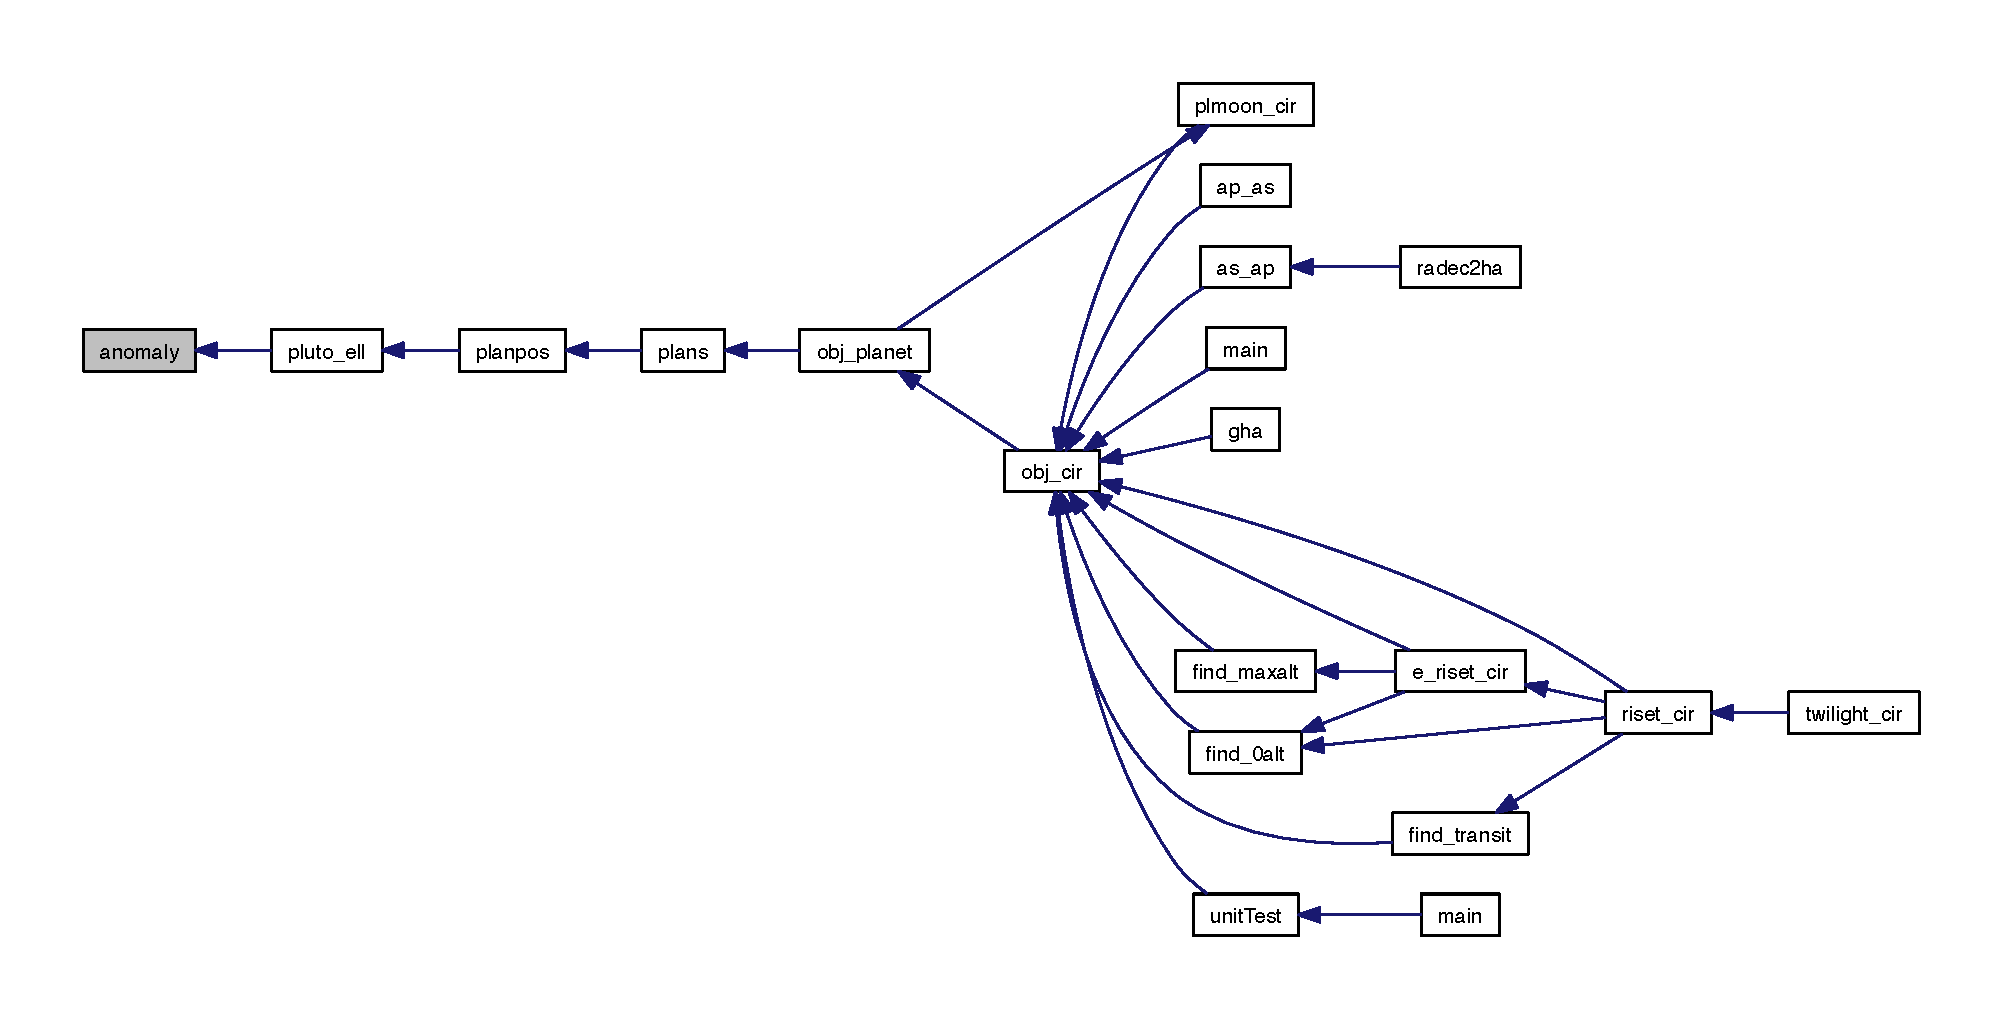
\includegraphics[width=350pt]{anomaly_8c_ab35408588a03873bb6cfc73b8b7aa349_icgraph}
\end{center}
\end{figure}




\subsection{Variable Documentation}
\hypertarget{anomaly_8c_ae037a79cb31f056d04153837887f5813}{\index{anomaly.\-c@{anomaly.\-c}!rcsid@{rcsid}}
\index{rcsid@{rcsid}!anomaly.c@{anomaly.\-c}}
\subsubsection[{rcsid}]{\setlength{\rightskip}{0pt plus 5cm}char$\ast$ rcsid\mbox{[}2\mbox{]} = \{(char $\ast$)rcsid, \char`\"{}@(\#) \$R\-C\-Sfile\-: {\bf anomaly.\-c},v \$ \$Date\-: 2003/03/20 08\-:51\-:37 \$ \$Revision\-: 1.\-3 \$ \$Name\-: \$\char`\"{}\}\hspace{0.3cm}{\ttfamily [static]}}}\label{anomaly_8c_ae037a79cb31f056d04153837887f5813}


Definition at line 63 of file anomaly.\-c.


\hypertarget{ap__as_8c}{\section{libastro/ap\-\_\-as.c File Reference}
\label{ap__as_8c}\index{libastro/ap\-\_\-as.\-c@{libastro/ap\-\_\-as.\-c}}
}
{\ttfamily \#include $<$string.\-h$>$}\\*
{\ttfamily \#include $<$math.\-h$>$}\\*
{\ttfamily \#include \char`\"{}astro.\-h\char`\"{}}\\*
Include dependency graph for ap\-\_\-as.\-c\-:
\nopagebreak
\begin{figure}[H]
\begin{center}
\leavevmode
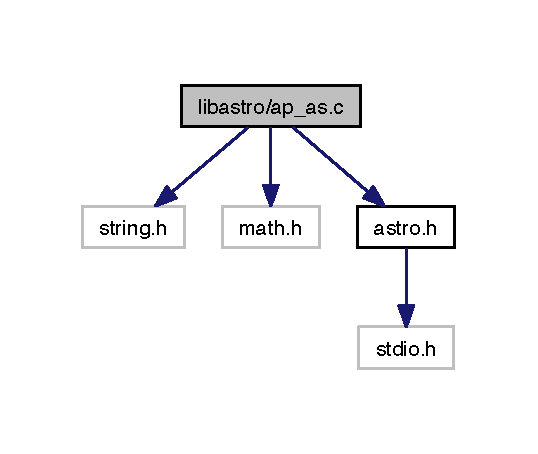
\includegraphics[width=258pt]{ap__as_8c__incl}
\end{center}
\end{figure}
\subsection*{Functions}
\begin{DoxyCompactItemize}
\item 
void \hyperlink{ap__as_8c_a11919b10760f866b904d4d154eede26e}{ap\-\_\-as} (\hyperlink{struct_now}{Now} $\ast$np, double Mjd, double $\ast$rap, double $\ast$decp)
\item 
void \hyperlink{ap__as_8c_a7aca2af85728e9b6336700b2753c6790}{as\-\_\-ap} (\hyperlink{struct_now}{Now} $\ast$np, double Mjd, double $\ast$rap, double $\ast$decp)
\end{DoxyCompactItemize}
\subsection*{Variables}
\begin{DoxyCompactItemize}
\item 
static char $\ast$ \hyperlink{ap__as_8c_ae037a79cb31f056d04153837887f5813}{rcsid} \mbox{[}2\mbox{]} = \{(char $\ast$)rcsid, \char`\"{}@(\#) \$R\-C\-Sfile\-: \hyperlink{circum_8c_aafc737ea9ef91f59cf9acd287fb8d085}{ap\-\_\-as.\-c},v \$ \$Date\-: 2006/08/28 00\-:20\-:58 \$ \$Revision\-: 1.\-8 \$ \$Name\-: \$\char`\"{}\}
\end{DoxyCompactItemize}


\subsection{Function Documentation}
\hypertarget{ap__as_8c_a11919b10760f866b904d4d154eede26e}{\index{ap\-\_\-as.\-c@{ap\-\_\-as.\-c}!ap\-\_\-as@{ap\-\_\-as}}
\index{ap\-\_\-as@{ap\-\_\-as}!ap_as.c@{ap\-\_\-as.\-c}}
\subsubsection[{ap\-\_\-as}]{\setlength{\rightskip}{0pt plus 5cm}void ap\-\_\-as (
\begin{DoxyParamCaption}
\item[{{\bf Now} $\ast$}]{np, }
\item[{double}]{Mjd, }
\item[{double $\ast$}]{rap, }
\item[{double $\ast$}]{decp}
\end{DoxyParamCaption}
)}}\label{ap__as_8c_a11919b10760f866b904d4d154eede26e}


Definition at line 12 of file ap\-\_\-as.\-c.



Here is the call graph for this function\-:
\nopagebreak
\begin{figure}[H]
\begin{center}
\leavevmode
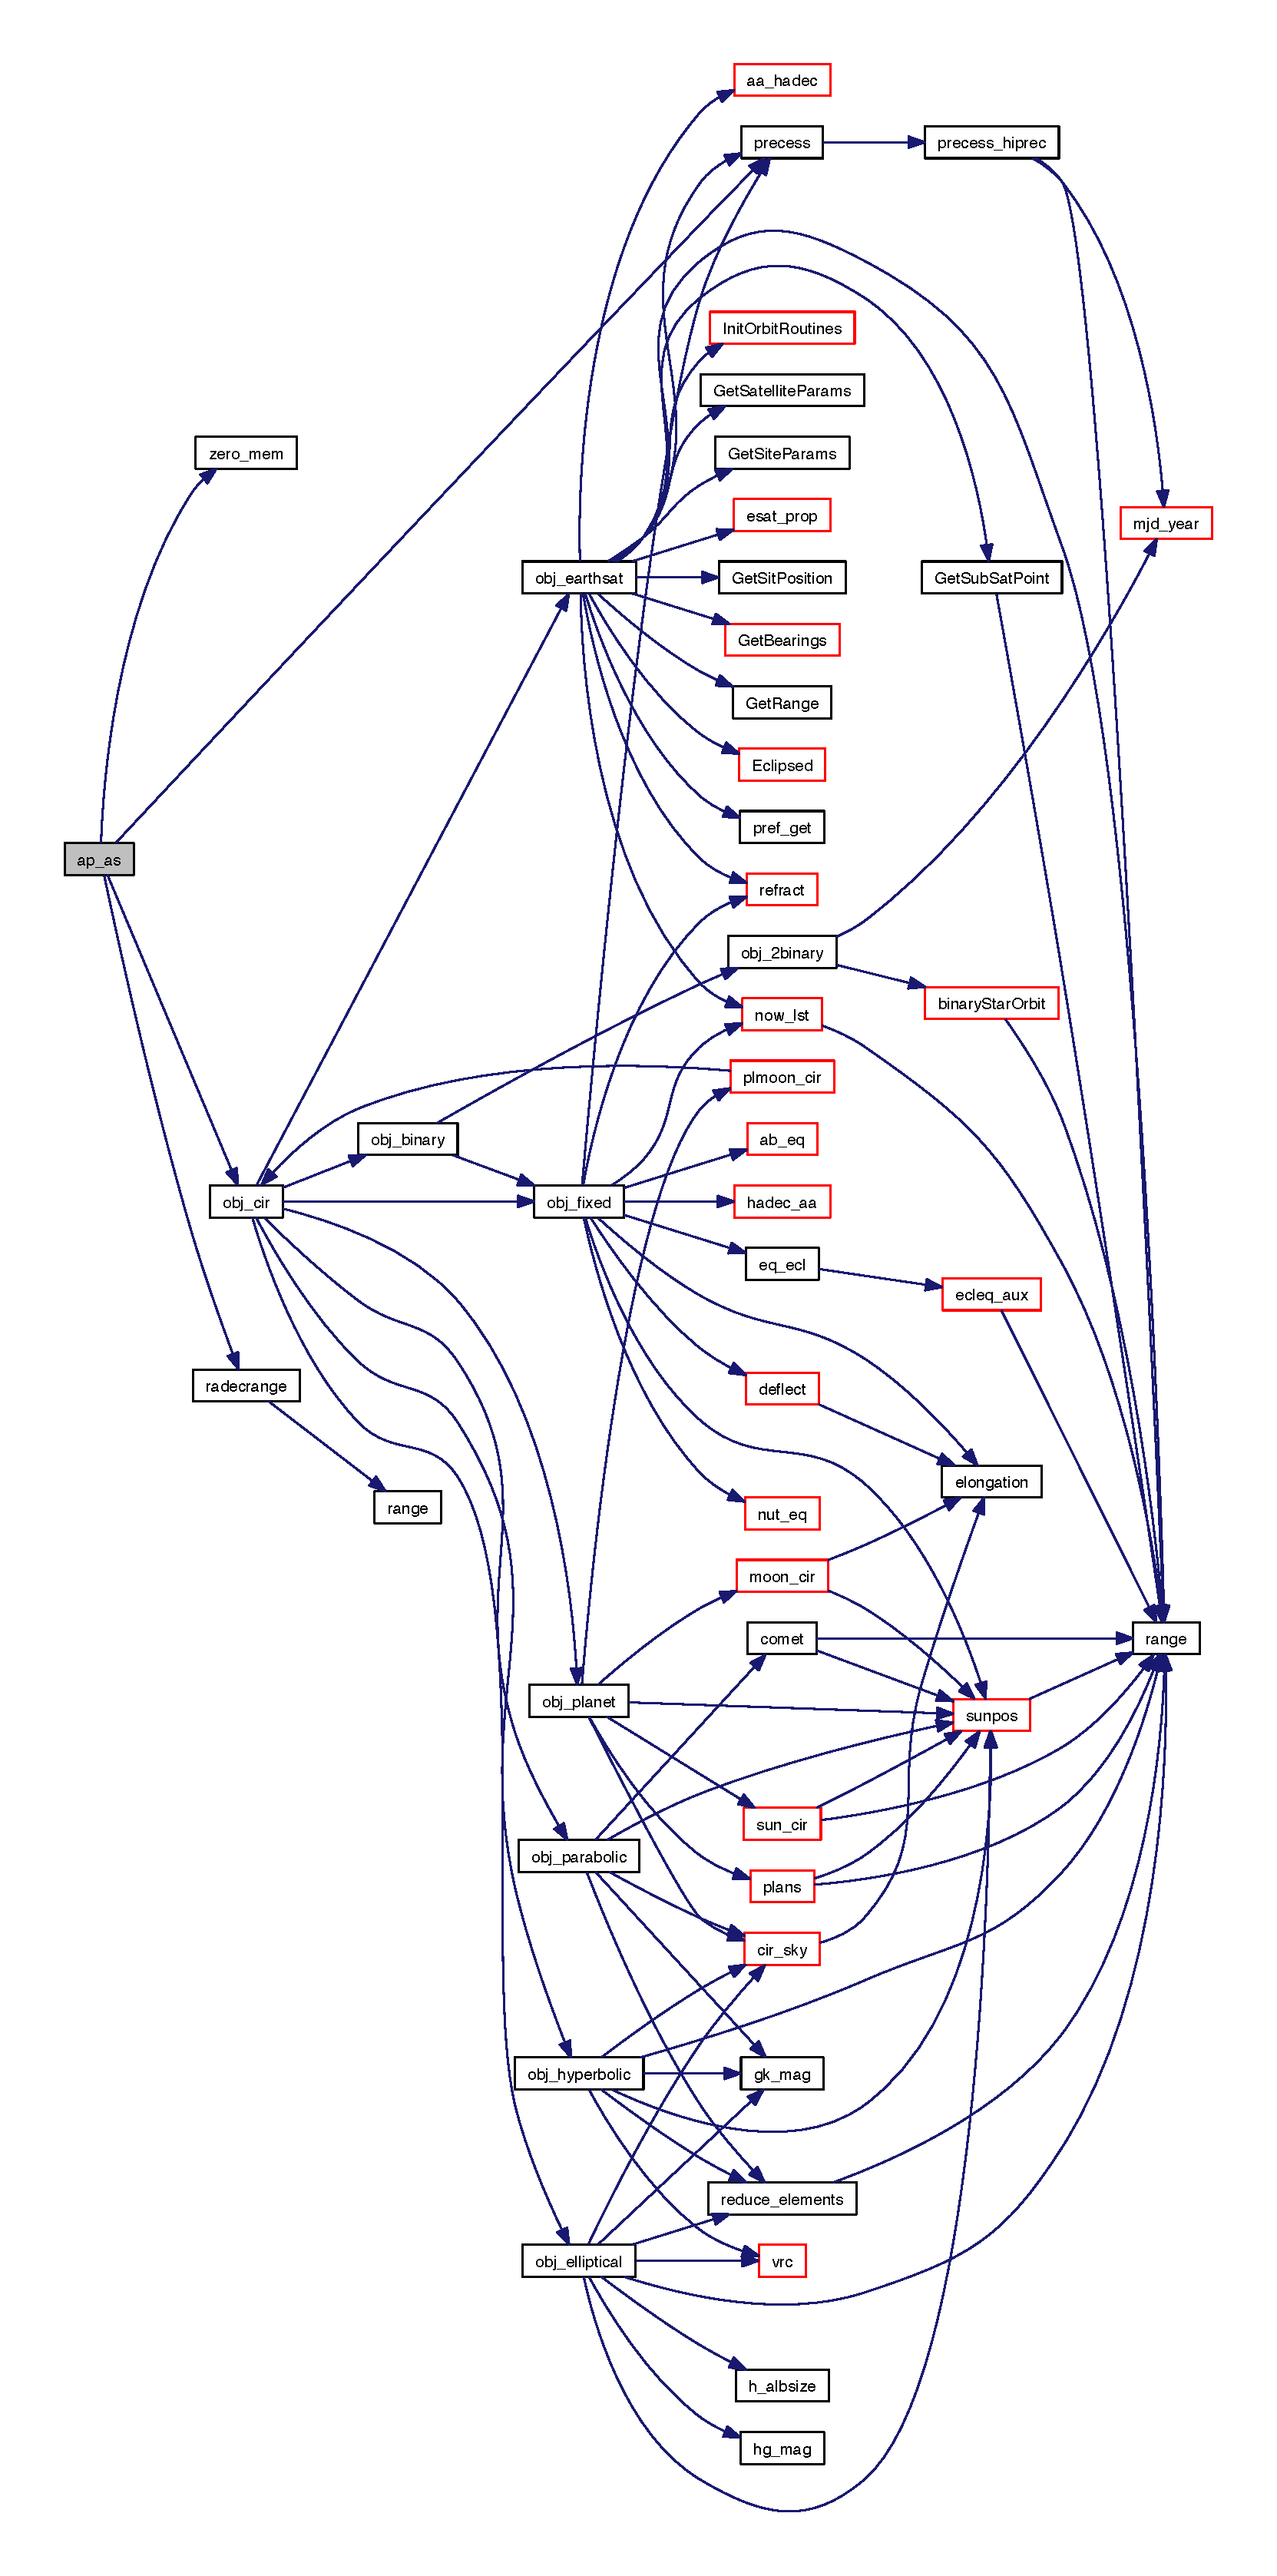
\includegraphics[height=550pt]{ap__as_8c_a11919b10760f866b904d4d154eede26e_cgraph}
\end{center}
\end{figure}


\hypertarget{ap__as_8c_a7aca2af85728e9b6336700b2753c6790}{\index{ap\-\_\-as.\-c@{ap\-\_\-as.\-c}!as\-\_\-ap@{as\-\_\-ap}}
\index{as\-\_\-ap@{as\-\_\-ap}!ap_as.c@{ap\-\_\-as.\-c}}
\subsubsection[{as\-\_\-ap}]{\setlength{\rightskip}{0pt plus 5cm}void as\-\_\-ap (
\begin{DoxyParamCaption}
\item[{{\bf Now} $\ast$}]{np, }
\item[{double}]{Mjd, }
\item[{double $\ast$}]{rap, }
\item[{double $\ast$}]{decp}
\end{DoxyParamCaption}
)}}\label{ap__as_8c_a7aca2af85728e9b6336700b2753c6790}


Definition at line 50 of file ap\-\_\-as.\-c.



Here is the call graph for this function\-:
\nopagebreak
\begin{figure}[H]
\begin{center}
\leavevmode
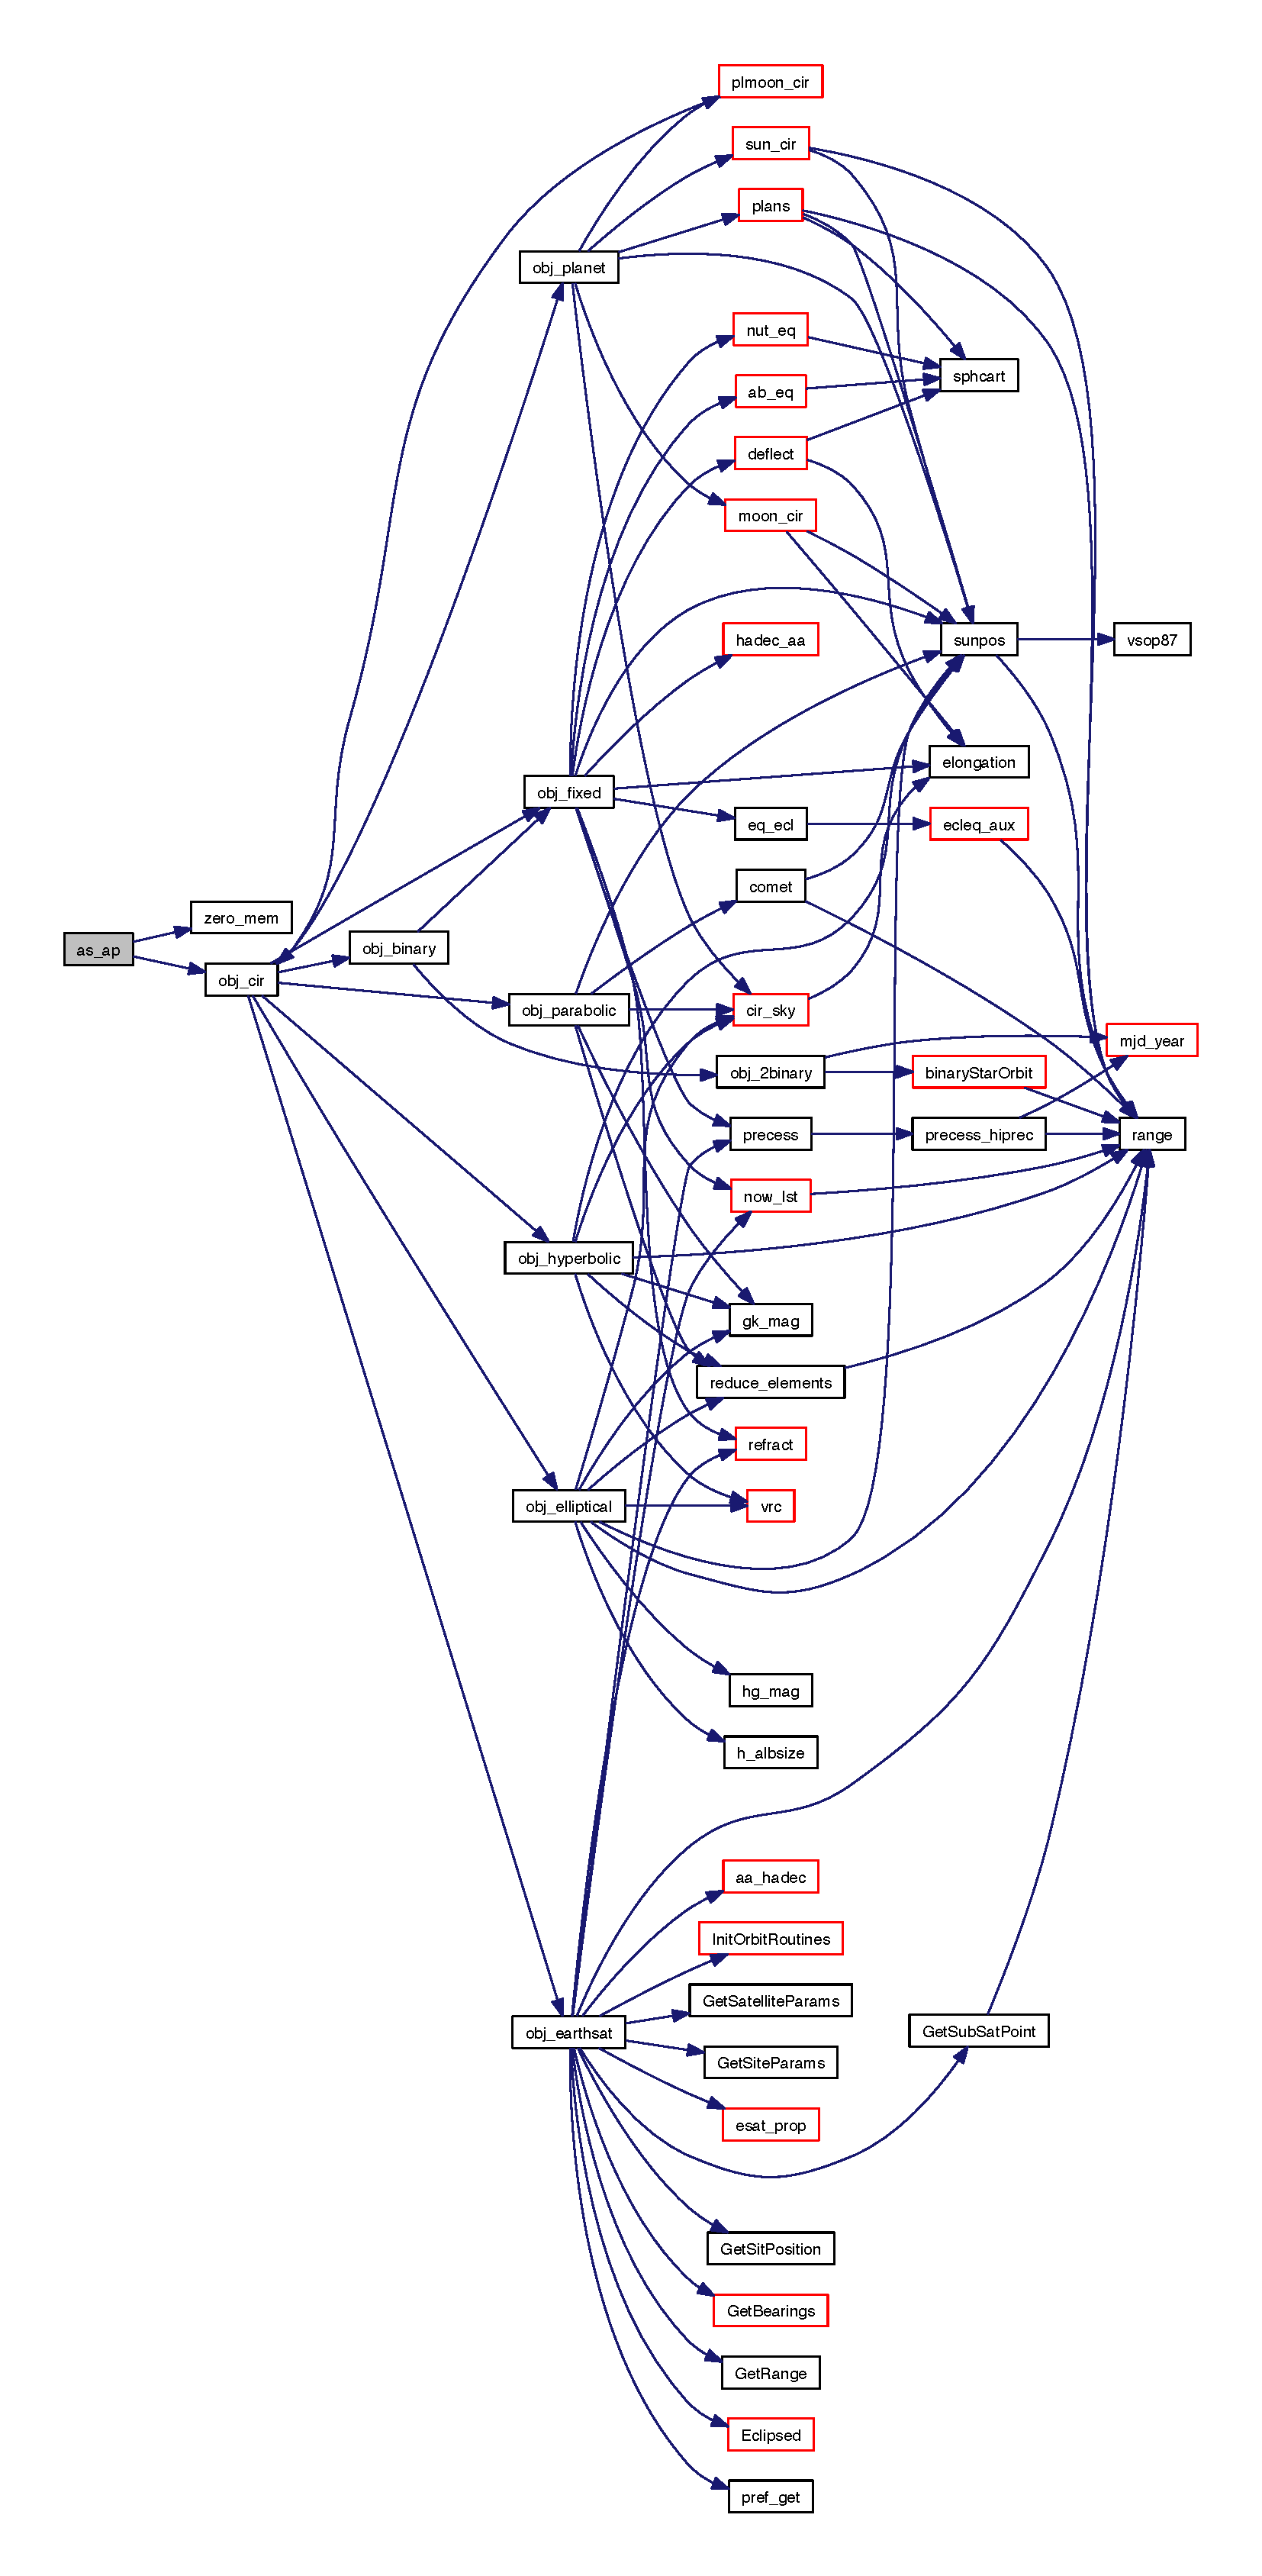
\includegraphics[height=550pt]{ap__as_8c_a7aca2af85728e9b6336700b2753c6790_cgraph}
\end{center}
\end{figure}




Here is the caller graph for this function\-:
\nopagebreak
\begin{figure}[H]
\begin{center}
\leavevmode
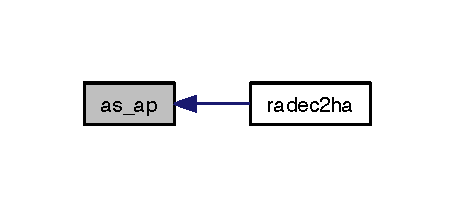
\includegraphics[width=218pt]{ap__as_8c_a7aca2af85728e9b6336700b2753c6790_icgraph}
\end{center}
\end{figure}




\subsection{Variable Documentation}
\hypertarget{ap__as_8c_ae037a79cb31f056d04153837887f5813}{\index{ap\-\_\-as.\-c@{ap\-\_\-as.\-c}!rcsid@{rcsid}}
\index{rcsid@{rcsid}!ap_as.c@{ap\-\_\-as.\-c}}
\subsubsection[{rcsid}]{\setlength{\rightskip}{0pt plus 5cm}char$\ast$ rcsid\mbox{[}2\mbox{]} = \{(char $\ast$)rcsid, \char`\"{}@(\#) \$R\-C\-Sfile\-: {\bf ap\-\_\-as.\-c},v \$ \$Date\-: 2006/08/28 00\-:20\-:58 \$ \$Revision\-: 1.\-8 \$ \$Name\-: \$\char`\"{}\}\hspace{0.3cm}{\ttfamily [static]}}}\label{ap__as_8c_ae037a79cb31f056d04153837887f5813}


Definition at line 68 of file ap\-\_\-as.\-c.


\hypertarget{astro_8h}{\section{libastro/astro.h File Reference}
\label{astro_8h}\index{libastro/astro.\-h@{libastro/astro.\-h}}
}
{\ttfamily \#include $<$stdio.\-h$>$}\\*
Include dependency graph for astro.\-h\-:
\nopagebreak
\begin{figure}[H]
\begin{center}
\leavevmode
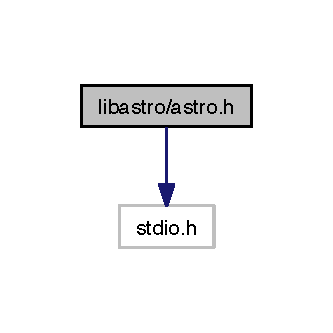
\includegraphics[width=160pt]{astro_8h__incl}
\end{center}
\end{figure}
This graph shows which files directly or indirectly include this file\-:
\nopagebreak
\begin{figure}[H]
\begin{center}
\leavevmode

\includegraphics[width=350pt]{astro_8h__dep__incl}
\end{center}
\end{figure}
\subsection*{Data Structures}
\begin{DoxyCompactItemize}
\item 
struct \hyperlink{struct_now}{Now}
\item 
struct \hyperlink{struct_mag}{Mag}
\item 
struct \hyperlink{struct_obj_any}{Obj\-Any}
\item 
struct \hyperlink{struct_obj_s_s}{Obj\-S\-S}
\item 
struct \hyperlink{struct_obj_f}{Obj\-F}
\item 
struct \hyperlink{struct_bin_orbit}{Bin\-Orbit}
\item 
struct \hyperlink{struct_bin_pos}{Bin\-Pos}
\item 
struct \hyperlink{struct_obj_b}{Obj\-B}
\item 
struct \hyperlink{struct_obj_pl}{Obj\-Pl}
\item 
struct \hyperlink{struct_obj_e}{Obj\-E}
\item 
struct \hyperlink{struct_obj_h}{Obj\-H}
\item 
struct \hyperlink{struct_obj_p}{Obj\-P}
\item 
struct \hyperlink{struct_obj_e_s}{Obj\-E\-S}
\item 
union \hyperlink{union_obj}{Obj}
\item 
struct \hyperlink{struct_rise_set}{Rise\-Set}
\item 
struct \hyperlink{struct_moon_data}{Moon\-Data}
\end{DoxyCompactItemize}
\subsection*{Macros}
\begin{DoxyCompactItemize}
\item 
\#define \hyperlink{astro_8h_a598a3330b3c21701223ee0ca14316eca}{P\-I}~3.\-141592653589793
\item 
\#define \hyperlink{astro_8h_a4f290ef8550589b60e07c92fe19e06cd}{degrad}(x)~((x)$\ast$\hyperlink{twobody_8c_a598a3330b3c21701223ee0ca14316eca}{P\-I}/180.)
\item 
\#define \hyperlink{astro_8h_a14e9da27d3ef91d14d3f049dc591f220}{raddeg}(x)~((x)$\ast$180./\hyperlink{twobody_8c_a598a3330b3c21701223ee0ca14316eca}{P\-I})
\item 
\#define \hyperlink{astro_8h_ae118c4a78016f5ff238c297ee568bfe1}{hrdeg}(x)~((x)$\ast$15.)
\item 
\#define \hyperlink{astro_8h_a23e7b5b636d7d8a44548f25b991a0562}{deghr}(x)~((x)/15.)
\item 
\#define \hyperlink{astro_8h_a6decddc4963c95defff0266089716730}{hrrad}(x)~\hyperlink{astro_8h_a4f290ef8550589b60e07c92fe19e06cd}{degrad}(\hyperlink{astro_8h_ae118c4a78016f5ff238c297ee568bfe1}{hrdeg}(x))
\item 
\#define \hyperlink{astro_8h_a64bcc0020d85100174c95e50e916b15a}{radhr}(x)~\hyperlink{astro_8h_a23e7b5b636d7d8a44548f25b991a0562}{deghr}(\hyperlink{astro_8h_a14e9da27d3ef91d14d3f049dc591f220}{raddeg}(x))
\item 
\#define \hyperlink{astro_8h_a339259d0a0e3e4de8593894ac41b2313}{S\-I\-D\-R\-A\-T\-E}~.\-9972695677
\item 
\#define \hyperlink{astro_8h_a17c22d077b2c872fa05d3482ea45caac}{M\-J\-D0}~2415020.\-0
\item 
\#define \hyperlink{astro_8h_afd09200b4253bfff7b9a890591e09292}{J2000}~(2451545.\-0 -\/ \hyperlink{astro_8h_a17c22d077b2c872fa05d3482ea45caac}{M\-J\-D0})      /$\ast$ yes, 2000 January 1 at 12h $\ast$/
\item 
\#define \hyperlink{astro_8h_a3fee30674709bf7cf2601f2e499372cf}{S\-P\-D}~(24.\-0$\ast$3600.\-0)	/$\ast$ seconds per day $\ast$/
\item 
\#define \hyperlink{astro_8h_a7557387e45810961ee3cd28325824c7a}{M\-A\-U}~(1.\-4959787e11)	/$\ast$ m / au $\ast$/
\item 
\#define \hyperlink{astro_8h_ad0b65ec0520704459f81adcd9b3bfd9e}{L\-T\-A\-U}~499.\-005		/$\ast$ seconds light takes to travel 1 A\-U $\ast$/
\item 
\#define \hyperlink{astro_8h_ac05ee1b3197f351a084ba3cc9c4a209e}{E\-R\-A\-D}~(6.\-37816e6)	/$\ast$ earth equitorial radius, m $\ast$/
\item 
\#define \hyperlink{astro_8h_a337cb0c78f1d499fd8aa81a37b42f12e}{M\-R\-A\-D}~(1.\-740e6)	/$\ast$ moon equitorial radius, m $\ast$/
\item 
\#define \hyperlink{astro_8h_a8f26fd9f2eaef9bce4fcddaf753071b2}{S\-R\-A\-D}~(6.\-95e8)	/$\ast$ sun equitorial radius, m $\ast$/
\item 
\#define \hyperlink{astro_8h_a29960b76786a31a4e7f1dceadad9484a}{F\-T\-P\-M}~3.\-28084		/$\ast$ ft per \hyperlink{moonnf_8c_a0da0a4863fcd4c1f629fc7fc6e6a4dad}{m} $\ast$/
\item 
\#define \hyperlink{astro_8h_a15315568b23fd0ed71c9e598c5479bcd}{E\-S\-A\-T\-\_\-\-M\-A\-G}~2	/$\ast$ default satellite magnitude $\ast$/
\item 
\#define \hyperlink{astro_8h_af164ea015f59ccf102e491ad38f91039}{F\-A\-S\-T\-\_\-\-S\-A\-T\-\_\-\-R\-P\-D}~0.\-25	/$\ast$ max earth sat rev/day considered \char`\"{}fast\char`\"{} $\ast$/
\item 
\#define \hyperlink{astro_8h_aadfef2133d5ca6910927f6970409757a}{E\-O\-D}~(-\/9786)		/$\ast$ special \hyperlink{astro_8h_a4c24e0950312168f5850003ab500781c}{epoch} flag\-: use \hyperlink{astro_8h_a4c24e0950312168f5850003ab500781c}{epoch} of date $\ast$/
\item 
\#define \hyperlink{astro_8h_ac251477d3eccad937eaee9382c458a54}{mjd}~np-\/$>$n\-\_\-mjd
\item 
\#define \hyperlink{astro_8h_ab5d040dac43192670c3e01def1373714}{lat}~np-\/$>$n\-\_\-lat
\item 
\#define \hyperlink{astro_8h_ab97e38355833c469f5594714736e2492}{lng}~np-\/$>$n\-\_\-lng
\item 
\#define \hyperlink{astro_8h_aa990489b3ee70b6559eb8bf3da0831f6}{tz}~np-\/$>$n\-\_\-tz
\item 
\#define \hyperlink{astro_8h_a5905d48604152cf57aa6bfa087b49173}{temp}~np-\/$>$n\-\_\-temp
\item 
\#define \hyperlink{astro_8h_a90ef800f5a07e95c920b0c41f83b8a83}{pressure}~np-\/$>$n\-\_\-pressure
\item 
\#define \hyperlink{astro_8h_aefadc5fcf8b90d116fe741b4a53f8bc2}{elev}~np-\/$>$n\-\_\-elev
\item 
\#define \hyperlink{astro_8h_aaab00957fa136736b0c2df6b5f97e689}{dip}~np-\/$>$n\-\_\-dip
\item 
\#define \hyperlink{astro_8h_a4c24e0950312168f5850003ab500781c}{epoch}~np-\/$>$n\-\_\-epoch
\item 
\#define \hyperlink{astro_8h_ab049f379bda0c1debfe19e9cce29ef78}{tznm}~np-\/$>$n\-\_\-tznm
\item 
\#define \hyperlink{astro_8h_a18dd39b8c91751aad12d89959e97adfd}{mjed}~\hyperlink{auxil_8c_a56ed70df83f91389b30f9f219fc20a2c}{mm\-\_\-mjed}(np)
\item 
\#define \hyperlink{astro_8h_a31021f1b77f916735a5e8bf4b50791ee}{M\-A\-G\-\_\-\-H\-G}~0       /$\ast$ using 0 makes H\-G the initial default $\ast$/
\item 
\#define \hyperlink{astro_8h_af749c3011548f2b8664f178f6dede939}{M\-A\-G\-\_\-gk}~1
\item 
\#define \hyperlink{astro_8h_a458557cd990d4a2729cb7903f6974e4c}{M\-A\-G\-S\-C\-A\-L\-E}~100.\-0
\item 
\#define \hyperlink{astro_8h_a82c893a7ea6253775028986a8e46d486}{set\-\_\-smag}(op, \hyperlink{moonnf_8c_a0da0a4863fcd4c1f629fc7fc6e6a4dad}{m})~((op)-\/$>$\hyperlink{astro_8h_ac46810f440573cbda4b300c17ba5451e}{s\-\_\-mag} = (short)floor((\hyperlink{moonnf_8c_a0da0a4863fcd4c1f629fc7fc6e6a4dad}{m})$\ast$\hyperlink{astro_8h_a458557cd990d4a2729cb7903f6974e4c}{M\-A\-G\-S\-C\-A\-L\-E} + 0.\-5))
\item 
\#define \hyperlink{astro_8h_a6bcfef436e5333f45947496d4038998e}{set\-\_\-fmag}(op, \hyperlink{moonnf_8c_a0da0a4863fcd4c1f629fc7fc6e6a4dad}{m})~((op)-\/$>$\hyperlink{astro_8h_a1ceb1a9f11396716c55e1ea11077750e}{f\-\_\-mag} = (short)floor((\hyperlink{moonnf_8c_a0da0a4863fcd4c1f629fc7fc6e6a4dad}{m})$\ast$\hyperlink{astro_8h_a458557cd990d4a2729cb7903f6974e4c}{M\-A\-G\-S\-C\-A\-L\-E} + 0.\-5))
\item 
\#define \hyperlink{astro_8h_a22d3705b08d8fc5d3bd0905d1093ca4a}{get\-\_\-mag}(op)~((op)-\/$>$\hyperlink{astro_8h_ac46810f440573cbda4b300c17ba5451e}{s\-\_\-mag} / \hyperlink{astro_8h_a458557cd990d4a2729cb7903f6974e4c}{M\-A\-G\-S\-C\-A\-L\-E})
\item 
\#define \hyperlink{astro_8h_a3f0c0ca2567b92718e065d6960f5b1d3}{get\-\_\-fmag}(op)~((op)-\/$>$\hyperlink{astro_8h_a1ceb1a9f11396716c55e1ea11077750e}{f\-\_\-mag} / \hyperlink{astro_8h_a458557cd990d4a2729cb7903f6974e4c}{M\-A\-G\-S\-C\-A\-L\-E})
\item 
\#define \hyperlink{astro_8h_a26811676b2cbf5d687ff3e45be6ebbc8}{M\-A\-X\-N\-M}~21
\item 
\#define \hyperlink{astro_8h_a0325bf42bbe8a6314a9e0b12e528750b}{O\-B\-J\-\_\-\-C\-O\-M\-M\-O\-N\-\_\-\-F\-L\-D\-S}
\item 
\#define \hyperlink{astro_8h_ae9e9e6f4befc4953ede9fddf1781eade}{O\-B\-J\-\_\-\-S\-O\-L\-S\-Y\-S\-\_\-\-F\-L\-D\-S}
\item 
\#define \hyperlink{astro_8h_a9fd6b91a020642cb3625e7c223eccbb2}{O\-B\-J\-\_\-\-F\-I\-X\-E\-D\-\_\-\-F\-L\-D\-S}
\item 
\#define \hyperlink{astro_8h_ae71358c16a25f35949f4b21cb745790f}{M\-A\-X\-B\-I\-N\-P\-O\-S}~2	/$\ast$ max discrete epochs to store when no elements $\ast$/
\item 
\#define \hyperlink{astro_8h_aa2afb569ac7e5f1c50bb3d06cac1b55d}{fo\-\_\-mag}~co\-\_\-mag	/$\ast$ pseudonym for so\-\_\-mag since it is not computed $\ast$/
\item 
\#define \hyperlink{astro_8h_a08fe41746df9944d37e14d7765e6a89c}{fo\-\_\-size}~co\-\_\-size	/$\ast$ pseudonym for so\-\_\-size since it is not computed $\ast$/
\item 
\#define \hyperlink{astro_8h_a374f72dda40eca8739307632edbc81ab}{S\-R\-S\-C\-A\-L\-E}~255.\-0		/$\ast$ galaxy size ratio scale $\ast$/
\item 
\#define \hyperlink{astro_8h_a8a6661277c6c9c71441756adf3201b92}{P\-A\-S\-C\-A\-L\-E}~(255.\-0/(2$\ast$\hyperlink{twobody_8c_a598a3330b3c21701223ee0ca14316eca}{P\-I}))	/$\ast$ pos angle scale factor $\ast$/
\item 
\#define \hyperlink{astro_8h_a09b45117e19ca6ff394bc0a04bdd0655}{get\-\_\-ratio}(op)~(((int)(op)-\/$>$\hyperlink{astro_8h_aa3bb0fcc0bdacb725af6f5d87992bd3c}{f\-\_\-ratio})/\hyperlink{astro_8h_a374f72dda40eca8739307632edbc81ab}{S\-R\-S\-C\-A\-L\-E})
\item 
\#define \hyperlink{astro_8h_afa7a6534302fe037b2b82925e1484850}{set\-\_\-ratio}(op, maj, min)
\item 
\#define \hyperlink{astro_8h_a45f780dca678f5f5ee84edd04c0624c6}{get\-\_\-pa}(op)~((double)(op)-\/$>$\hyperlink{astro_8h_a9c1bffbd16752ff2c9dff4d3b34897a4}{f\-\_\-pa}/\hyperlink{astro_8h_a8a6661277c6c9c71441756adf3201b92}{P\-A\-S\-C\-A\-L\-E})
\item 
\#define \hyperlink{astro_8h_a2b3eb3d719411e547b6b2ad22f90df93}{set\-\_\-pa}(op, s)~((op)-\/$>$\hyperlink{astro_8h_a9c1bffbd16752ff2c9dff4d3b34897a4}{f\-\_\-pa} = (\hyperlink{astro_8h_a0c8186d9b9b7880309c27230bbb5e69d}{byte})((s)$\ast$\hyperlink{astro_8h_a8a6661277c6c9c71441756adf3201b92}{P\-A\-S\-C\-A\-L\-E} + 0.\-5))
\item 
\#define \hyperlink{astro_8h_a2ed957184ded3d1a8b6fed065b1cbe4b}{N\-C\-L\-A\-S\-S\-E\-S}~128 /$\ast$ \hyperlink{atlas_8c_a76f11d9a0a47b94f72c2d0e77fb32240}{n} potential fo\-\_\-classes -\/-\/ allow for all A\-S\-C\-I\-I $\ast$/
\item 
\#define \hyperlink{astro_8h_a48c0d537d616c4cbc8dca877ffd4d042}{F\-U\-S\-E\-R0}~0x01
\item 
\#define \hyperlink{astro_8h_a706235faaf123f74486336dae4c0064e}{F\-U\-S\-E\-R1}~0x02
\item 
\#define \hyperlink{astro_8h_a05744378a551584a8f3ac09e4030dee7}{F\-U\-S\-E\-R2}~0x04
\item 
\#define \hyperlink{astro_8h_ac3ff6d196c7f006688d567cd70a27d16}{F\-U\-S\-E\-R3}~0x08
\item 
\#define \hyperlink{astro_8h_af960c036bc5c2c53cab7d7558764acd8}{F\-U\-S\-E\-R4}~0x10
\item 
\#define \hyperlink{astro_8h_acdc887c41fb6097951c22e5f169cc205}{F\-U\-S\-E\-R5}~0x20
\item 
\#define \hyperlink{astro_8h_a50b5dcec59cb476a872a4724a9b068b0}{F\-U\-S\-E\-R6}~0x40
\item 
\#define \hyperlink{astro_8h_ac9ca7315416f91322ca2d2811fb5041f}{F\-U\-S\-E\-R7}~0x80
\item 
\#define \hyperlink{astro_8h_a330f4d42b52a3b43493ca96ac3f533f3}{F\-L\-D\-S\-T\-A\-R}~\hyperlink{astro_8h_ac3ff6d196c7f006688d567cd70a27d16}{F\-U\-S\-E\-R3}
\item 
\#define \hyperlink{astro_8h_ae6a409c9e61d5623e6c8b5986936b859}{N\-O\-C\-I\-R\-C\-U\-M}~\hyperlink{astro_8h_ac9ca7315416f91322ca2d2811fb5041f}{F\-U\-S\-E\-R7}
\item 
\#define \hyperlink{astro_8h_aa4d460b75825255aa2d86a7bdb89a9bf}{o\-\_\-type}~any.\-co\-\_\-type
\item 
\#define \hyperlink{astro_8h_a6e24a43b9adfbb3aa0bce49d3289af0a}{o\-\_\-name}~any.\-co\-\_\-name
\item 
\#define \hyperlink{astro_8h_a7c3004ea726b65b35c8b6d5ca347ae3f}{o\-\_\-flags}~any.\-co\-\_\-flags
\item 
\#define \hyperlink{astro_8h_a59e093ddab315fbaa191f2d94af660cf}{o\-\_\-age}~any.\-co\-\_\-age
\item 
\#define \hyperlink{astro_8h_a88c52b0f5138bd5dec43abd14079cb80}{s\-\_\-ra}~any.\-co\-\_\-ra
\item 
\#define \hyperlink{astro_8h_acf76ca483317f2ed745ed64c6fa0e250}{s\-\_\-dec}~any.\-co\-\_\-dec
\item 
\#define \hyperlink{astro_8h_a23fe29cb74d4b900cac4222171cc4c09}{s\-\_\-gaera}~any.\-co\-\_\-gaera
\item 
\#define \hyperlink{astro_8h_a6c70fe914a113daed5e6b54b2741b7bb}{s\-\_\-gaedec}~any.\-co\-\_\-gaedec
\item 
\#define \hyperlink{astro_8h_ae38afb419abe7b5a06096eaf7b95d54c}{s\-\_\-az}~any.\-co\-\_\-az
\item 
\#define \hyperlink{astro_8h_a5b82aae89c214fcfdc7e14b3574005a9}{s\-\_\-alt}~any.\-co\-\_\-alt
\item 
\#define \hyperlink{astro_8h_ac0cea80a3859369ab8515ac400597ea7}{s\-\_\-elong}~any.\-co\-\_\-elong
\item 
\#define \hyperlink{astro_8h_ab1511090cdcf8fc6d8c0b80f38e95856}{s\-\_\-size}~any.\-co\-\_\-size
\item 
\#define \hyperlink{astro_8h_ac46810f440573cbda4b300c17ba5451e}{s\-\_\-mag}~any.\-co\-\_\-mag
\item 
\#define \hyperlink{astro_8h_a43a3efce2c06f414f59a1d1719145e9b}{s\-\_\-sdist}~anyss.\-so\-\_\-sdist
\item 
\#define \hyperlink{astro_8h_a4ba36f67cdc0e5f01831a4b688b40cf6}{s\-\_\-edist}~anyss.\-so\-\_\-edist
\item 
\#define \hyperlink{astro_8h_a33fc7786b51dede6f6eb257fd7b09bc0}{s\-\_\-hlong}~anyss.\-so\-\_\-hlong
\item 
\#define \hyperlink{astro_8h_ae50e688f986d07a60a3be1ac4d75dcd5}{s\-\_\-hlat}~anyss.\-so\-\_\-hlat
\item 
\#define \hyperlink{astro_8h_a50af373c994a8d453adebd7dc5caa053}{s\-\_\-phase}~anyss.\-so\-\_\-phase
\item 
\#define \hyperlink{astro_8h_ad684b582e96e10f683b3f4e1490cb784}{s\-\_\-elev}~es.\-ess\-\_\-elev
\item 
\#define \hyperlink{astro_8h_aa9584143783ffc9dc7d60ebc0ee93822}{s\-\_\-range}~es.\-ess\-\_\-range
\item 
\#define \hyperlink{astro_8h_ada4ad7331e78770e041090ae0ffff53d}{s\-\_\-rangev}~es.\-ess\-\_\-rangev
\item 
\#define \hyperlink{astro_8h_ac5f643b560cab75e23ddf44c164522f3}{s\-\_\-sublat}~es.\-ess\-\_\-sublat
\item 
\#define \hyperlink{astro_8h_ae55788447ae9b297d83eff08bba280cd}{s\-\_\-sublng}~es.\-ess\-\_\-sublng
\item 
\#define \hyperlink{astro_8h_a0718a3e605470f303e5ba6dd8e431f1a}{s\-\_\-eclipsed}~es.\-ess\-\_\-eclipsed
\item 
\#define \hyperlink{astro_8h_ad1aaedbf16c0fa870ca6b5e002253a2b}{f\-\_\-class}~f.\-fo\-\_\-class
\item 
\#define \hyperlink{astro_8h_ae06a6f74b32c16463083d6b1c2e69479}{f\-\_\-spect}~f.\-fo\-\_\-spect
\item 
\#define \hyperlink{astro_8h_aa3bb0fcc0bdacb725af6f5d87992bd3c}{f\-\_\-ratio}~f.\-fo\-\_\-ratio
\item 
\#define \hyperlink{astro_8h_a9c1bffbd16752ff2c9dff4d3b34897a4}{f\-\_\-pa}~f.\-fo\-\_\-pa
\item 
\#define \hyperlink{astro_8h_aa3f15a20d4878b4e545956815dd958ad}{f\-\_\-epoch}~f.\-fo\-\_\-epoch
\item 
\#define \hyperlink{astro_8h_a8eaea87023c8e358015d3a54cb18b654}{f\-\_\-\-R\-A}~f.\-fo\-\_\-ra
\item 
\#define \hyperlink{astro_8h_a01dd206b89f1e008314d0792f9c7572a}{f\-\_\-pm\-R\-A}~f.\-fo\-\_\-pmra
\item 
\#define \hyperlink{astro_8h_a090b3e18d661f917568dc8d524174974}{f\-\_\-dec}~f.\-fo\-\_\-dec
\item 
\#define \hyperlink{astro_8h_a4b07406c73abe53efdc8b1e8bd06dff8}{f\-\_\-pmdec}~f.\-fo\-\_\-pmdec
\item 
\#define \hyperlink{astro_8h_a1ceb1a9f11396716c55e1ea11077750e}{f\-\_\-mag}~\hyperlink{astro_8h_aa2afb569ac7e5f1c50bb3d06cac1b55d}{f.\-fo\-\_\-mag}
\item 
\#define \hyperlink{astro_8h_a7a6c8bbb9618d8207e5ece24cbeb7dd8}{f\-\_\-size}~\hyperlink{astro_8h_a08fe41746df9944d37e14d7765e6a89c}{f.\-fo\-\_\-size}
\item 
\#define \hyperlink{astro_8h_ae376d882d02f0d6180e60d19f08e609e}{e\-\_\-cepoch}~e.\-eo\-\_\-cepoch
\item 
\#define \hyperlink{astro_8h_a229d129dc1bc9d33e47d8784a3dc1067}{e\-\_\-epoch}~e.\-eo\-\_\-epoch
\item 
\#define \hyperlink{astro_8h_ae52d2c69b5930fe978d334cd6a88ff33}{e\-\_\-startok}~e.\-eo\-\_\-startok
\item 
\#define \hyperlink{astro_8h_a806920e5d0b431c0c3bfa6890c49689b}{e\-\_\-endok}~e.\-eo\-\_\-endok
\item 
\#define \hyperlink{astro_8h_ac2e714d19aabbb9480c5e6ca37ca2382}{e\-\_\-inc}~e.\-eo\-\_\-inc
\item 
\#define \hyperlink{astro_8h_a19e6fde0c6aef514974fa46948db81cd}{e\-\_\-\-Om}~e.\-eo\-\_\-\-Om
\item 
\#define \hyperlink{astro_8h_adf26fc82f62588f39655d35f52536ffa}{e\-\_\-om}~e.\-eo\-\_\-om
\item 
\#define \hyperlink{astro_8h_aa4d778733b85a101fe5eca8bd2f83529}{e\-\_\-a}~e.\-eo\-\_\-a
\item 
\#define \hyperlink{astro_8h_ab702265dcbc97082662fe81c7f9bccb2}{e\-\_\-e}~e.\-eo\-\_\-e
\item 
\#define \hyperlink{astro_8h_ac754a3117cea7cb766f8502ee01772f7}{e\-\_\-\-M}~e.\-eo\-\_\-\-M
\item 
\#define \hyperlink{astro_8h_a736baa4b38e1bb4cc3654b85f1d81b3b}{e\-\_\-size}~e.\-eo\-\_\-size
\item 
\#define \hyperlink{astro_8h_a2e56f5a881827efa3e4ac5c058b861cf}{e\-\_\-mag}~e.\-eo\-\_\-mag
\item 
\#define \hyperlink{astro_8h_acfa9643c32c5aa168b46034ae3362160}{h\-\_\-epoch}~h.\-ho\-\_\-epoch
\item 
\#define \hyperlink{astro_8h_add1910d52059deb5c31cf32e6096eb73}{h\-\_\-startok}~h.\-ho\-\_\-startok
\item 
\#define \hyperlink{astro_8h_aba7f977bd3bc3d191bc8c33f223e008e}{h\-\_\-endok}~h.\-ho\-\_\-endok
\item 
\#define \hyperlink{astro_8h_a4550021606496e21cd6bfc71e67f1f6e}{h\-\_\-ep}~h.\-ho\-\_\-ep
\item 
\#define \hyperlink{astro_8h_abc1790cf8da85931058674cad95a21e3}{h\-\_\-inc}~h.\-ho\-\_\-inc
\item 
\#define \hyperlink{astro_8h_af9cadcbb840737176b1d7f3b1eb9bdf1}{h\-\_\-\-Om}~h.\-ho\-\_\-\-Om
\item 
\#define \hyperlink{astro_8h_a6e7ab4443735a29db6245a431fa08c26}{h\-\_\-om}~h.\-ho\-\_\-om
\item 
\#define \hyperlink{astro_8h_a3464cdf57953ded536bfd8fcefcb4a6f}{h\-\_\-e}~h.\-ho\-\_\-e
\item 
\#define \hyperlink{astro_8h_a4960a8d3568b48f1e5c6c5bbf317d2fd}{h\-\_\-qp}~h.\-ho\-\_\-qp
\item 
\#define \hyperlink{astro_8h_a00f8317cb2bbbb5d632ea919bbbcce63}{h\-\_\-g}~h.\-ho\-\_\-g
\item 
\#define \hyperlink{astro_8h_af0d9d9b940860a5887604cfd18c273e1}{h\-\_\-k}~h.\-ho\-\_\-k
\item 
\#define \hyperlink{astro_8h_af621ff4c1cf8fef1df24449df441713a}{h\-\_\-size}~h.\-ho\-\_\-size
\item 
\#define \hyperlink{astro_8h_a8572bac21b2fcaa27135da208581a305}{p\-\_\-epoch}~p.\-po\-\_\-epoch
\item 
\#define \hyperlink{astro_8h_a7122abf0a28d14977135baa8e5e6560d}{p\-\_\-startok}~p.\-po\-\_\-startok
\item 
\#define \hyperlink{astro_8h_a1d046c01ce236ba275c9f6f5c893ecff}{p\-\_\-endok}~p.\-po\-\_\-endok
\item 
\#define \hyperlink{astro_8h_ac45e1e0f4cca0461597e4be58467ecd6}{p\-\_\-ep}~p.\-po\-\_\-ep
\item 
\#define \hyperlink{astro_8h_a039704364f9934bc9797fa1c66e731b7}{p\-\_\-inc}~p.\-po\-\_\-inc
\item 
\#define \hyperlink{astro_8h_a70e63b2b04f96510bc11fa73c1e73eab}{p\-\_\-qp}~p.\-po\-\_\-qp
\item 
\#define \hyperlink{astro_8h_a0431ff164f02bba454dd38539e02c262}{p\-\_\-om}~p.\-po\-\_\-om
\item 
\#define \hyperlink{astro_8h_a06d342b724ea9f3315a8761aefb2e186}{p\-\_\-\-Om}~p.\-po\-\_\-\-Om
\item 
\#define \hyperlink{astro_8h_a15d64c863c6ad50a90f8a0a44cb2b407}{p\-\_\-g}~p.\-po\-\_\-g
\item 
\#define \hyperlink{astro_8h_a74c47bf86b9573cf1b618c2d96a82bb7}{p\-\_\-k}~p.\-po\-\_\-k
\item 
\#define \hyperlink{astro_8h_aab7283e1766701945a0229c8a356fe3f}{p\-\_\-size}~p.\-po\-\_\-size
\item 
\#define \hyperlink{astro_8h_aa67b0b514f83a71d817997e7dc8b5b5f}{es\-\_\-epoch}~es.\-eso\-\_\-epoch
\item 
\#define \hyperlink{astro_8h_a3f3539ac4db30514561ab26df4f4dbd4}{es\-\_\-startok}~es.\-eso\-\_\-startok
\item 
\#define \hyperlink{astro_8h_ab49a6f18b0389ee60388fdca67e858d4}{es\-\_\-endok}~es.\-eso\-\_\-endok
\item 
\#define \hyperlink{astro_8h_aa71b7aa3331aafeb1c1c86c26055e2fa}{es\-\_\-inc}~es.\-eso\-\_\-inc
\item 
\#define \hyperlink{astro_8h_aca951aeec56d3414794f1af585d2d33b}{es\-\_\-raan}~es.\-eso\-\_\-raan
\item 
\#define \hyperlink{astro_8h_ab1ced82d29674ff13a876369255ac783}{es\-\_\-e}~es.\-eso\-\_\-e
\item 
\#define \hyperlink{astro_8h_aac01c40c086ab58f00012be4d638df7c}{es\-\_\-ap}~es.\-eso\-\_\-ap
\item 
\#define \hyperlink{astro_8h_ad76354ec6b712a78199d73645b32bd7a}{es\-\_\-\-M}~es.\-eso\-\_\-\-M
\item 
\#define \hyperlink{astro_8h_a497056dc43ee9af32b7910eb0965df94}{es\-\_\-n}~es.\-eso\-\_\-n
\item 
\#define \hyperlink{astro_8h_ab26a3f5792c1a214e856568cafd1cd9e}{es\-\_\-decay}~es.\-eso\-\_\-decay
\item 
\#define \hyperlink{astro_8h_ae4d728dbf3871403ba6f1c0f9d0300c9}{es\-\_\-drag}~es.\-eso\-\_\-drag
\item 
\#define \hyperlink{astro_8h_aca05a3570275df3508c6f2af6882ddb7}{es\-\_\-orbit}~es.\-eso\-\_\-orbit
\item 
\#define \hyperlink{astro_8h_ac8475d861ac77f99a2481f6cd9bf009b}{pl\-\_\-code}~pl.\-plo\-\_\-code
\item 
\#define \hyperlink{astro_8h_a36662e3b3ca1b1a54e0d4c9542303937}{pl\-\_\-moon}~pl.\-plo\-\_\-moon
\item 
\#define \hyperlink{astro_8h_aade26bee74208e1e2eb0ea0f4e46a4ed}{pl\-\_\-evis}~pl.\-plo\-\_\-evis
\item 
\#define \hyperlink{astro_8h_a7534cde2bb2d1e5696cc9aa574172801}{pl\-\_\-svis}~pl.\-plo\-\_\-svis
\item 
\#define \hyperlink{astro_8h_ad292b6983d7cb8501ddbeae890cfd791}{pl\-\_\-x}~pl.\-plo\-\_\-x
\item 
\#define \hyperlink{astro_8h_ab8eccb6563746cde3da0d5e3e4cd4f8b}{pl\-\_\-y}~pl.\-plo\-\_\-y
\item 
\#define \hyperlink{astro_8h_a693c4eb41bd7393c3439f0659c5c4ae1}{pl\-\_\-z}~pl.\-plo\-\_\-z
\item 
\#define \hyperlink{astro_8h_ac66b61108441009fd5ec156cf6f3e17a}{pl\-\_\-aux1}~pl.\-plo\-\_\-aux1
\item 
\#define \hyperlink{astro_8h_a9f8f469aee1c7a43818641028ddcd835}{pl\-\_\-aux2}~pl.\-plo\-\_\-aux2
\item 
\#define \hyperlink{astro_8h_a1339078188969a144692da6f16356ca8}{b\-\_\-2compute}~b.\-b\-\_\-2compute
\item 
\#define \hyperlink{astro_8h_a751ca9a91eb871cd86b02279618ecd75}{b\-\_\-2spect}~b.\-b\-\_\-2spect
\item 
\#define \hyperlink{astro_8h_ae108310000b33de13274fb5bb7beeffb}{b\-\_\-2mag}~b.\-b\-\_\-2mag
\item 
\#define \hyperlink{astro_8h_a241a26c6c0401f55e8e41200e4e152a8}{b\-\_\-bo}~b.\-u.\-b\-\_\-bo
\item 
\#define \hyperlink{astro_8h_a326447a174850a0b911e6019c636afee}{b\-\_\-bp}~b.\-u.\-b\-\_\-bp
\item 
\#define \hyperlink{astro_8h_a2e3127c8c0aa24abb3bd35e7f8fe5cd9}{b\-\_\-nbp}~b.\-b\-\_\-nbp
\item 
\#define \hyperlink{astro_8h_a3302e8745576939ae7887d6bdad13937}{O\-B\-J\-T\-Y\-P\-E2\-M\-A\-S\-K}(t)~(1$<$$<$(t))
\item 
\#define \hyperlink{astro_8h_a8c6e2cff30345ba1bc359aa843ae08d6}{F\-I\-X\-E\-D\-M}~\hyperlink{astro_8h_a3302e8745576939ae7887d6bdad13937}{O\-B\-J\-T\-Y\-P\-E2\-M\-A\-S\-K}(\hyperlink{astro_8h_a21ada50c882656c2a4723dde25f56d4aa9b5eccb7f8f027c46f2018d07c74f384}{F\-I\-X\-E\-D})
\item 
\#define \hyperlink{astro_8h_a7911cb8621a8bd4403cea554531a13c5}{B\-I\-N\-A\-R\-Y\-S\-T\-A\-R\-M}~\hyperlink{astro_8h_a3302e8745576939ae7887d6bdad13937}{O\-B\-J\-T\-Y\-P\-E2\-M\-A\-S\-K}(\hyperlink{astro_8h_a21ada50c882656c2a4723dde25f56d4aa7a30a935b97f376b1c22695e6a83c993}{B\-I\-N\-A\-R\-Y\-S\-T\-A\-R})
\item 
\#define \hyperlink{astro_8h_abdb4745aea6540dc811709d5550f398e}{E\-L\-L\-I\-P\-T\-I\-C\-A\-L\-M}~\hyperlink{astro_8h_a3302e8745576939ae7887d6bdad13937}{O\-B\-J\-T\-Y\-P\-E2\-M\-A\-S\-K}(\hyperlink{astro_8h_a21ada50c882656c2a4723dde25f56d4aac6bcc2946fcd74ccf710812b92b8875a}{E\-L\-L\-I\-P\-T\-I\-C\-A\-L})
\item 
\#define \hyperlink{astro_8h_a8cdca67e09f961e2275cce0942fbf653}{H\-Y\-P\-E\-R\-B\-O\-L\-I\-C\-M}~\hyperlink{astro_8h_a3302e8745576939ae7887d6bdad13937}{O\-B\-J\-T\-Y\-P\-E2\-M\-A\-S\-K}(\hyperlink{astro_8h_a21ada50c882656c2a4723dde25f56d4aad7b12016a7a43c287f88e56a8d3e9550}{H\-Y\-P\-E\-R\-B\-O\-L\-I\-C})
\item 
\#define \hyperlink{astro_8h_ad96ece423218566db175cc782cc1734c}{P\-A\-R\-A\-B\-O\-L\-I\-C\-M}~\hyperlink{astro_8h_a3302e8745576939ae7887d6bdad13937}{O\-B\-J\-T\-Y\-P\-E2\-M\-A\-S\-K}(\hyperlink{astro_8h_a21ada50c882656c2a4723dde25f56d4aa6aaa4cbf733e3a4c6556b1f2ff8840a9}{P\-A\-R\-A\-B\-O\-L\-I\-C})
\item 
\#define \hyperlink{astro_8h_af4358234847ef84c8221828dc4fd3bb8}{E\-A\-R\-T\-H\-S\-A\-T\-M}~\hyperlink{astro_8h_a3302e8745576939ae7887d6bdad13937}{O\-B\-J\-T\-Y\-P\-E2\-M\-A\-S\-K}(\hyperlink{astro_8h_a21ada50c882656c2a4723dde25f56d4aa10f8ec1a64299d5c71fd586543294eb5}{E\-A\-R\-T\-H\-S\-A\-T})
\item 
\#define \hyperlink{astro_8h_a676bde761bdfa53d03f5e1e8fbee23fa}{P\-L\-A\-N\-E\-T\-M}~\hyperlink{astro_8h_a3302e8745576939ae7887d6bdad13937}{O\-B\-J\-T\-Y\-P\-E2\-M\-A\-S\-K}(\hyperlink{astro_8h_a21ada50c882656c2a4723dde25f56d4aa71085833d5414e6afbae581f3b792dc8}{P\-L\-A\-N\-E\-T})
\item 
\#define \hyperlink{astro_8h_ab6948f9a6aeab5f006b241b90e05cdd0}{A\-L\-L\-M}~($\sim$0)
\item 
\#define \hyperlink{astro_8h_a9d5d2fe2b683c0fe0c0c7a443abbe452}{R\-S\-\_\-\-N\-O\-R\-I\-S\-E}~0x0001	/$\ast$ object does not rise as such today $\ast$/
\item 
\#define \hyperlink{astro_8h_a279f1ddf7b739cc7ba754bcbc7ecb8ba}{R\-S\-\_\-\-N\-O\-S\-E\-T}~0x0002	/$\ast$ object does not set as such today $\ast$/
\item 
\#define \hyperlink{astro_8h_a2726888175bc810c782af118a4dee4c9}{R\-S\-\_\-\-N\-O\-T\-R\-A\-N\-S}~0x0004	/$\ast$ object does not transit as such today $\ast$/
\item 
\#define \hyperlink{astro_8h_aa74acc5ea8fad74bce3358828bfe9627}{R\-S\-\_\-\-C\-I\-R\-C\-U\-M\-P\-O\-L\-A\-R}~0x0010	/$\ast$ object stays up all day today $\ast$/
\item 
\#define \hyperlink{astro_8h_a1908ac344fdbedb1dfa0c19e068f5dd9}{R\-S\-\_\-\-N\-E\-V\-E\-R\-U\-P}~0x0020	/$\ast$ object never up at all today $\ast$/
\item 
\#define \hyperlink{astro_8h_a9c5922cc8c392ae3543d9f4a906f6cea}{R\-S\-\_\-\-E\-R\-R\-O\-R}~0x1000	/$\ast$ can't figure out anything! $\ast$/
\item 
\#define \hyperlink{astro_8h_a9709d65b70000b233aba1a616a84b291}{R\-S\-\_\-\-R\-I\-S\-E\-R\-R}~(0x0100$\vert$\-R\-S\-\_\-\-E\-R\-R\-O\-R) /$\ast$ error computing rise $\ast$/
\item 
\#define \hyperlink{astro_8h_aa244564b6d5a0599f75d2a937a34d3a6}{R\-S\-\_\-\-S\-E\-T\-E\-R\-R}~(0x0200$\vert$\-R\-S\-\_\-\-E\-R\-R\-O\-R) /$\ast$ error computing set $\ast$/
\item 
\#define \hyperlink{astro_8h_ae72c5310ee9bcbcfb13d2bc1df300202}{R\-S\-\_\-\-T\-R\-A\-N\-S\-E\-R\-R}~(0x0400$\vert$\-R\-S\-\_\-\-E\-R\-R\-O\-R) /$\ast$ error computing transit $\ast$/
\item 
\#define \hyperlink{astro_8h_a813ba7946895d411deb5649bbd71ec1e}{is\-\_\-type}(op, \hyperlink{moonnf_8c_a0da0a4863fcd4c1f629fc7fc6e6a4dad}{m})~(\hyperlink{astro_8h_a3302e8745576939ae7887d6bdad13937}{O\-B\-J\-T\-Y\-P\-E2\-M\-A\-S\-K}((op)-\/$>$\hyperlink{astro_8h_aa4d460b75825255aa2d86a7bdb89a9bf}{o\-\_\-type}) \& (\hyperlink{moonnf_8c_a0da0a4863fcd4c1f629fc7fc6e6a4dad}{m}))
\item 
\#define \hyperlink{astro_8h_ad1b6ec090d5ed1b3b2061000b6bdc906}{is\-\_\-planet}(op, p)~(\hyperlink{astro_8h_a813ba7946895d411deb5649bbd71ec1e}{is\-\_\-type}(op,\hyperlink{astro_8h_a676bde761bdfa53d03f5e1e8fbee23fa}{P\-L\-A\-N\-E\-T\-M}) \&\& op-\/$>$\hyperlink{astro_8h_ac8475d861ac77f99a2481f6cd9bf009b}{pl\-\_\-code} == (p))
\item 
\#define \hyperlink{astro_8h_aa5d80d2813d76fb12822ec62fdba0687}{is\-\_\-ssobj}(op)~\hyperlink{astro_8h_a813ba7946895d411deb5649bbd71ec1e}{is\-\_\-type}(op,\hyperlink{astro_8h_a676bde761bdfa53d03f5e1e8fbee23fa}{P\-L\-A\-N\-E\-T\-M}$\vert$\hyperlink{astro_8h_a8cdca67e09f961e2275cce0942fbf653}{H\-Y\-P\-E\-R\-B\-O\-L\-I\-C\-M}$\vert$\hyperlink{astro_8h_ad96ece423218566db175cc782cc1734c}{P\-A\-R\-A\-B\-O\-L\-I\-C\-M}$\vert$\hyperlink{astro_8h_abdb4745aea6540dc811709d5550f398e}{E\-L\-L\-I\-P\-T\-I\-C\-A\-L\-M})
\item 
\#define \hyperlink{astro_8h_a070944892f635e1c5865ff0c0a79223f}{X\-\_\-\-M\-A\-X\-N\-M\-O\-O\-N\-S}~\hyperlink{astro_8h_a5878d29a6316d7d762b6326a0949faafa3058927e9687af8253fc6ec7cce9cc3e}{S\-\_\-\-N\-M\-O\-O\-N\-S}		/$\ast$ N.\-B. chosen by hand $\ast$/
\item 
\#define \hyperlink{astro_8h_ac5cded70557e19515ee4438a77c2884f}{N\-C\-N\-S}~89
\end{DoxyCompactItemize}
\subsection*{Typedefs}
\begin{DoxyCompactItemize}
\item 
typedef unsigned char \hyperlink{astro_8h_ae672b2b5ac326921aa475fa826b072ba}{Obj\-Type\-\_\-t}
\item 
typedef unsigned char \hyperlink{astro_8h_a5e6b41594eab21893fc3248d9ecd74c2}{Obj\-Age\-\_\-t}
\item 
typedef unsigned char \hyperlink{astro_8h_a0c8186d9b9b7880309c27230bbb5e69d}{byte}
\end{DoxyCompactItemize}
\subsection*{Enumerations}
\begin{DoxyCompactItemize}
\item 
enum \hyperlink{astro_8h_a2a6f493a094887058ce904937bb27647}{P\-L\-Code} \{ \\*
\hyperlink{astro_8h_a2a6f493a094887058ce904937bb27647a2a817d820a01a599d5a7b8d4c1efdcd1}{M\-E\-R\-C\-U\-R\-Y}, 
\hyperlink{astro_8h_a2a6f493a094887058ce904937bb27647a3cad57d681b42e9c2cad588c91fdfe86}{V\-E\-N\-U\-S}, 
\hyperlink{astro_8h_a2a6f493a094887058ce904937bb27647a83bbeb6e2f14b3da41dfd9c0387d253f}{M\-A\-R\-S}, 
\hyperlink{astro_8h_a2a6f493a094887058ce904937bb27647a8a6646a7e2b61b5c5618a3f7fe85f753}{J\-U\-P\-I\-T\-E\-R}, 
\\*
\hyperlink{astro_8h_a2a6f493a094887058ce904937bb27647a2eebce8d3bf5836b06a77fa835b4fe6f}{S\-A\-T\-U\-R\-N}, 
\hyperlink{astro_8h_a2a6f493a094887058ce904937bb27647a3e928779f4d4e6121eb8b8a9b75ff0c9}{U\-R\-A\-N\-U\-S}, 
\hyperlink{astro_8h_a2a6f493a094887058ce904937bb27647a519e60bb67177b86592a42967c226690}{N\-E\-P\-T\-U\-N\-E}, 
\hyperlink{astro_8h_a2a6f493a094887058ce904937bb27647ab345c5970ddbe5fe989958760dac118e}{P\-L\-U\-T\-O}, 
\\*
\hyperlink{astro_8h_a2a6f493a094887058ce904937bb27647ad740e028dfaa7a9a6bcd70b41b2d6598}{S\-U\-N}, 
\hyperlink{astro_8h_a2a6f493a094887058ce904937bb27647a913c111f07d4331db94d8a5f4e5f0bc8}{M\-O\-O\-N}, 
\hyperlink{astro_8h_a2a6f493a094887058ce904937bb27647ad51498f3267f8b12e29941d0b378c643}{N\-O\-B\-J}
 \}
\item 
enum \hyperlink{astro_8h_ac0d9b5d3144a9cf8616c62dad3579db7}{M\-Code} \{ \\*
\hyperlink{astro_8h_ac0d9b5d3144a9cf8616c62dad3579db7aa68e1f172492990f60dd1bc45c292f71}{X\-\_\-\-P\-L\-A\-N\-E\-T} = 0, 
\hyperlink{astro_8h_ac0d9b5d3144a9cf8616c62dad3579db7a1933b67b544085153ac600d3a1ef00e6}{P\-H\-O\-B\-O\-S} = N\-O\-B\-J, 
\hyperlink{astro_8h_ac0d9b5d3144a9cf8616c62dad3579db7a431dfed3109c5f06e5b5fe1d8123f9f0}{D\-E\-I\-M\-O\-S}, 
\hyperlink{astro_8h_ac0d9b5d3144a9cf8616c62dad3579db7aedd9974ef2207e0a03e0717dcb9e2269}{I\-O}, 
\\*
\hyperlink{astro_8h_ac0d9b5d3144a9cf8616c62dad3579db7a7855e26aab3183575b5c5bc4f03a7573}{E\-U\-R\-O\-P\-A}, 
\hyperlink{astro_8h_ac0d9b5d3144a9cf8616c62dad3579db7aca42cd5e60f06e5e184535ba1a592bb8}{G\-A\-N\-Y\-M\-E\-D\-E}, 
\hyperlink{astro_8h_ac0d9b5d3144a9cf8616c62dad3579db7abf891e500d6db7b2d086a306f6cf3e0c}{C\-A\-L\-L\-I\-S\-T\-O}, 
\hyperlink{astro_8h_ac0d9b5d3144a9cf8616c62dad3579db7a1cab80fbab18e82cbb2ec45afc3c8737}{M\-I\-M\-A\-S}, 
\\*
\hyperlink{astro_8h_ac0d9b5d3144a9cf8616c62dad3579db7af0549f68e334a8e2c571d29065d7d0bc}{E\-N\-C\-E\-L\-A\-D\-U\-S}, 
\hyperlink{astro_8h_ac0d9b5d3144a9cf8616c62dad3579db7ab5ffe67f3916df389a9b780b5cf390e9}{T\-E\-T\-H\-Y\-S}, 
\hyperlink{astro_8h_ac0d9b5d3144a9cf8616c62dad3579db7aaa35aeab0d4eb1a38bbe79d085d71b37}{D\-I\-O\-N\-E}, 
\hyperlink{astro_8h_ac0d9b5d3144a9cf8616c62dad3579db7a58c58ba3feba755a26fa2a752fa25e57}{R\-H\-E\-A}, 
\\*
\hyperlink{astro_8h_ac0d9b5d3144a9cf8616c62dad3579db7a35f0d23a5e13a3edc09320ac9ca20dff}{T\-I\-T\-A\-N}, 
\hyperlink{astro_8h_ac0d9b5d3144a9cf8616c62dad3579db7adff8ebc38d18ad0879934dc8804e84b8}{H\-Y\-P\-E\-R\-I\-O\-N}, 
\hyperlink{astro_8h_ac0d9b5d3144a9cf8616c62dad3579db7a63b32cad913d0baf3f897aeae478f9e1}{I\-A\-P\-E\-T\-U\-S}, 
\hyperlink{astro_8h_ac0d9b5d3144a9cf8616c62dad3579db7a76c8ae8d4ebc1f73bddb0c7f599b6d70}{A\-R\-I\-E\-L}, 
\\*
\hyperlink{astro_8h_ac0d9b5d3144a9cf8616c62dad3579db7a5c832550bbaa1a5879cc816b8f1557e0}{U\-M\-B\-R\-I\-E\-L}, 
\hyperlink{astro_8h_ac0d9b5d3144a9cf8616c62dad3579db7a8955211a0c5423a183c1fe62a8c534a3}{T\-I\-T\-A\-N\-I\-A}, 
\hyperlink{astro_8h_ac0d9b5d3144a9cf8616c62dad3579db7a5fdb0dc0264b2283628dd23fd6ce7197}{O\-B\-E\-R\-O\-N}, 
\hyperlink{astro_8h_ac0d9b5d3144a9cf8616c62dad3579db7a1830fb3e9a0a9f7006a741b4bc3199ed}{M\-I\-R\-A\-N\-D\-A}, 
\\*
\hyperlink{astro_8h_ac0d9b5d3144a9cf8616c62dad3579db7a19ec060f4bd05c6c95a15f8e0a7c92a7}{N\-B\-U\-I\-L\-T\-I\-N}
 \}
\item 
enum \hyperlink{astro_8h_a21ada50c882656c2a4723dde25f56d4a}{Obj\-Type} \{ \\*
\hyperlink{astro_8h_a21ada50c882656c2a4723dde25f56d4aaadfec66ebf4a626c173c6ec484621241}{U\-N\-D\-E\-F\-O\-B\-J} =0, 
\hyperlink{astro_8h_a21ada50c882656c2a4723dde25f56d4aa9b5eccb7f8f027c46f2018d07c74f384}{F\-I\-X\-E\-D}, 
\hyperlink{astro_8h_a21ada50c882656c2a4723dde25f56d4aa7a30a935b97f376b1c22695e6a83c993}{B\-I\-N\-A\-R\-Y\-S\-T\-A\-R}, 
\hyperlink{astro_8h_a21ada50c882656c2a4723dde25f56d4aac6bcc2946fcd74ccf710812b92b8875a}{E\-L\-L\-I\-P\-T\-I\-C\-A\-L}, 
\\*
\hyperlink{astro_8h_a21ada50c882656c2a4723dde25f56d4aad7b12016a7a43c287f88e56a8d3e9550}{H\-Y\-P\-E\-R\-B\-O\-L\-I\-C}, 
\hyperlink{astro_8h_a21ada50c882656c2a4723dde25f56d4aa6aaa4cbf733e3a4c6556b1f2ff8840a9}{P\-A\-R\-A\-B\-O\-L\-I\-C}, 
\hyperlink{astro_8h_a21ada50c882656c2a4723dde25f56d4aa10f8ec1a64299d5c71fd586543294eb5}{E\-A\-R\-T\-H\-S\-A\-T}, 
\hyperlink{astro_8h_a21ada50c882656c2a4723dde25f56d4aa71085833d5414e6afbae581f3b792dc8}{P\-L\-A\-N\-E\-T}, 
\\*
\hyperlink{astro_8h_a21ada50c882656c2a4723dde25f56d4aac02d945b64b0bf01819db6643f13841d}{N\-O\-B\-J\-T\-Y\-P\-E\-S}
 \}
\item 
enum \hyperlink{astro_8h_afaeec18bba1a4b2238c56ff864c7a674}{\-\_\-marsmoons} \{ \hyperlink{astro_8h_afaeec18bba1a4b2238c56ff864c7a674a53546844a154084357808c8b21366b88}{M\-\_\-\-M\-A\-R\-S} = 0, 
\hyperlink{astro_8h_afaeec18bba1a4b2238c56ff864c7a674af2282eab426256dd53dd289ffb93280e}{M\-\_\-\-P\-H\-O\-B\-O\-S}, 
\hyperlink{astro_8h_afaeec18bba1a4b2238c56ff864c7a674a54bc5c3ff2b8f2a84148dfef9af6aa7c}{M\-\_\-\-D\-E\-I\-M\-O\-S}, 
\hyperlink{astro_8h_afaeec18bba1a4b2238c56ff864c7a674ab48935852a8ec737103a71d2d6df9b83}{M\-\_\-\-N\-M\-O\-O\-N\-S}
 \}
\item 
enum \hyperlink{astro_8h_a68d8fcc7d6fb107812e1afbb4100a61f}{\-\_\-jupmoons} \{ \\*
\hyperlink{astro_8h_a68d8fcc7d6fb107812e1afbb4100a61fa73c736a3ced29790db752d36082bb2c9}{J\-\_\-\-J\-U\-P\-I\-T\-E\-R} = 0, 
\hyperlink{astro_8h_a68d8fcc7d6fb107812e1afbb4100a61fa94cf28bcf7ab27a308fb84a6ae2b83ce}{J\-\_\-\-I\-O}, 
\hyperlink{astro_8h_a68d8fcc7d6fb107812e1afbb4100a61faf1ac12d01d3b7197749a73f80a1fde5f}{J\-\_\-\-E\-U\-R\-O\-P\-A}, 
\hyperlink{astro_8h_a68d8fcc7d6fb107812e1afbb4100a61fa294271970d7f0a47b5d3ff57afb49305}{J\-\_\-\-G\-A\-N\-Y\-M\-E\-D\-E}, 
\\*
\hyperlink{astro_8h_a68d8fcc7d6fb107812e1afbb4100a61fa219b8ae262a0256d51c5eec2ecf6a1e9}{J\-\_\-\-C\-A\-L\-L\-I\-S\-T\-O}, 
\hyperlink{astro_8h_a68d8fcc7d6fb107812e1afbb4100a61fac735d88505905bf3ba8309a38e0ae7ef}{J\-\_\-\-N\-M\-O\-O\-N\-S}
 \}
\item 
enum \hyperlink{astro_8h_a5878d29a6316d7d762b6326a0949faaf}{\-\_\-satmoons} \{ \\*
\hyperlink{astro_8h_a5878d29a6316d7d762b6326a0949faafa7cdf4cc5e775a7688f4f2d1107dc87a9}{S\-\_\-\-S\-A\-T\-U\-R\-N} = 0, 
\hyperlink{astro_8h_a5878d29a6316d7d762b6326a0949faafaae3062c66fa9f8bb6e3e61aea5a830be}{S\-\_\-\-M\-I\-M\-A\-S}, 
\hyperlink{astro_8h_a5878d29a6316d7d762b6326a0949faafa3dc0f12b864c3719ee7539ce3d580a79}{S\-\_\-\-E\-N\-C\-E\-L\-A\-D\-U\-S}, 
\hyperlink{astro_8h_a5878d29a6316d7d762b6326a0949faafa348a15cba9d19a58584f2f7b464beaec}{S\-\_\-\-T\-E\-T\-H\-Y\-S}, 
\\*
\hyperlink{astro_8h_a5878d29a6316d7d762b6326a0949faafa9fd00212a9199ddbda395da011d1d976}{S\-\_\-\-D\-I\-O\-N\-E}, 
\hyperlink{astro_8h_a5878d29a6316d7d762b6326a0949faafa3b71503ed5de8f358865f6cbd1a63cbf}{S\-\_\-\-R\-H\-E\-A}, 
\hyperlink{astro_8h_a5878d29a6316d7d762b6326a0949faafae4cd3b709a5c9e41f7a214707d5eeea5}{S\-\_\-\-T\-I\-T\-A\-N}, 
\hyperlink{astro_8h_a5878d29a6316d7d762b6326a0949faafadae41bca9743ac3d0719d5d7348a6a2f}{S\-\_\-\-H\-Y\-P\-E\-R\-I\-O\-N}, 
\\*
\hyperlink{astro_8h_a5878d29a6316d7d762b6326a0949faafad051b2bfd312cc3f69a2e235d375e9a3}{S\-\_\-\-I\-A\-P\-E\-T\-U\-S}, 
\hyperlink{astro_8h_a5878d29a6316d7d762b6326a0949faafa3058927e9687af8253fc6ec7cce9cc3e}{S\-\_\-\-N\-M\-O\-O\-N\-S}
 \}
\item 
enum \hyperlink{astro_8h_a19cf1f394aeb15ac823c4343c241ea42}{\-\_\-uramoons} \{ \\*
\hyperlink{astro_8h_a19cf1f394aeb15ac823c4343c241ea42a262d38960a0c2873b74a65fd5f2c5400}{U\-\_\-\-U\-R\-A\-N\-U\-S} = 0, 
\hyperlink{astro_8h_a19cf1f394aeb15ac823c4343c241ea42a9cba1f103c01c9684153da99b81cd25c}{U\-\_\-\-A\-R\-I\-E\-L}, 
\hyperlink{astro_8h_a19cf1f394aeb15ac823c4343c241ea42a8b4f6ec59c9328aa6d94569400119371}{U\-\_\-\-U\-M\-B\-R\-I\-E\-L}, 
\hyperlink{astro_8h_a19cf1f394aeb15ac823c4343c241ea42a6d9686c5e62d3c668e5b0da7e3f39743}{U\-\_\-\-T\-I\-T\-A\-N\-I\-A}, 
\\*
\hyperlink{astro_8h_a19cf1f394aeb15ac823c4343c241ea42a49138e687d23dcebaaf984a792099ed5}{U\-\_\-\-O\-B\-E\-R\-O\-N}, 
\hyperlink{astro_8h_a19cf1f394aeb15ac823c4343c241ea42a2035172d8467259fcd982993e0bddf6f}{U\-\_\-\-M\-I\-R\-A\-N\-D\-A}, 
\hyperlink{astro_8h_a19cf1f394aeb15ac823c4343c241ea42a5e13c0a645171c94f216d7a68b67fa4d}{U\-\_\-\-N\-M\-O\-O\-N\-S}
 \}
\end{DoxyCompactItemize}
\subsection*{Functions}
\begin{DoxyCompactItemize}
\item 
void \hyperlink{astro_8h_afb4e9b19dfbf97eaf03b05111e9e919d}{aa\-\_\-hadec} (double lt, double alt, double az, double $\ast$ha, double $\ast$\hyperlink{constel_8c_a69b9a761071ef54b54c6970eb304268f}{dec})
\item 
void \hyperlink{astro_8h_a8ce2fb9152b3b6d728cda9ac4962378e}{hadec\-\_\-aa} (double lt, double ha, double \hyperlink{constel_8c_a69b9a761071ef54b54c6970eb304268f}{dec}, double $\ast$alt, double $\ast$az)
\item 
void \hyperlink{astro_8h_abef08d899770c40423cbf24280ab10cf}{ab\-\_\-ecl} (double \hyperlink{moonnf_8c_a0da0a4863fcd4c1f629fc7fc6e6a4dad}{m}, double lsn, double $\ast$lam, double $\ast$bet)
\item 
void \hyperlink{astro_8h_aee075aa543ef48c790c4b6b7c965db1b}{ab\-\_\-eq} (double \hyperlink{moonnf_8c_a0da0a4863fcd4c1f629fc7fc6e6a4dad}{m}, double lsn, double $\ast$\hyperlink{constel_8c_aeb704957d1ce8d0299718c60f3cd3a4c}{ra}, double $\ast$\hyperlink{constel_8c_a69b9a761071ef54b54c6970eb304268f}{dec})
\item 
void \hyperlink{astro_8h_a0149c681dca5872a5194adc30048833e}{airmass} (double aa, double $\ast$Xp)
\item 
void \hyperlink{astro_8h_ab35408588a03873bb6cfc73b8b7aa349}{anomaly} (double ma, double s, double $\ast$nu, double $\ast$ea)
\item 
void \hyperlink{astro_8h_a11919b10760f866b904d4d154eede26e}{ap\-\_\-as} (\hyperlink{struct_now}{Now} $\ast$np, double Mjd, double $\ast$rap, double $\ast$decp)
\item 
void \hyperlink{astro_8h_a7aca2af85728e9b6336700b2753c6790}{as\-\_\-ap} (\hyperlink{struct_now}{Now} $\ast$np, double Mjd, double $\ast$rap, double $\ast$decp)
\item 
char $\ast$ \hyperlink{astro_8h_ab8f78a0e6c0ea713b73c04f88e270480}{um\-\_\-atlas} (double \hyperlink{constel_8c_aeb704957d1ce8d0299718c60f3cd3a4c}{ra}, double \hyperlink{constel_8c_a69b9a761071ef54b54c6970eb304268f}{dec})
\item 
char $\ast$ \hyperlink{astro_8h_aefd0669ddbff5634f9d0fca4df003d52}{u2k\-\_\-atlas} (double \hyperlink{constel_8c_aeb704957d1ce8d0299718c60f3cd3a4c}{ra}, double \hyperlink{constel_8c_a69b9a761071ef54b54c6970eb304268f}{dec})
\item 
char $\ast$ \hyperlink{astro_8h_ad9b069df7c280a1584d54cd0be01c585}{msa\-\_\-atlas} (double \hyperlink{constel_8c_aeb704957d1ce8d0299718c60f3cd3a4c}{ra}, double \hyperlink{constel_8c_a69b9a761071ef54b54c6970eb304268f}{dec})
\item 
double \hyperlink{astro_8h_a56ed70df83f91389b30f9f219fc20a2c}{mm\-\_\-mjed} (\hyperlink{struct_now}{Now} $\ast$np)
\item 
int \hyperlink{astro_8h_a3c04fc909e750cb1784cadf3101bddcc}{chap95} (double \hyperlink{moonnf_8c_a0da0a4863fcd4c1f629fc7fc6e6a4dad}{m}, int obj, double prec, double $\ast$ret)
\item 
int \hyperlink{astro_8h_a88029bd0976d52e82ec40e1b9230d54a}{obj\-\_\-cir} (\hyperlink{struct_now}{Now} $\ast$np, \hyperlink{union_obj}{Obj} $\ast$op)
\item 
void \hyperlink{astro_8h_ae42663ccffbb2741a6b27abdfd032a72}{comet} (double \hyperlink{moonnf_8c_a0da0a4863fcd4c1f629fc7fc6e6a4dad}{m}, double ep, double inc, double ap, double qp, double om, double $\ast$lpd, double $\ast$psi, double $\ast$rp, double $\ast$rho, double $\ast$lam, double $\ast$bet)
\item 
int \hyperlink{astro_8h_a76033e94f3dda39f889bf9f0999e1287}{cns\-\_\-pick} (double r, double d, double e)
\item 
int \hyperlink{astro_8h_a2fa52e582fb3bc39427f1724a1945003}{cns\-\_\-id} (char $\ast$abbrev)
\item 
char $\ast$ \hyperlink{astro_8h_ac2ebcab9bbbcb07dd26dbcfc2e7a5571}{cns\-\_\-name} (int id)
\item 
int \hyperlink{astro_8h_a03e1b115ca90718115d025bc167ce6a8}{cns\-\_\-edges} (double e, double $\ast$$\ast$ra0p, double $\ast$$\ast$dec0p, double $\ast$$\ast$ra1p, double $\ast$$\ast$dec1p)
\item 
int \hyperlink{astro_8h_aa91f0872a2f28f469bddcb9463a7b023}{cns\-\_\-list} (double \hyperlink{constel_8c_aeb704957d1ce8d0299718c60f3cd3a4c}{ra}, double \hyperlink{constel_8c_a69b9a761071ef54b54c6970eb304268f}{dec}, double e, double rad, int ids\mbox{[}$\,$\mbox{]})
\item 
int \hyperlink{astro_8h_aa8601bb074905861837ddfda3f2bf0b1}{cns\-\_\-figure} (int id, double e, double \hyperlink{constel_8c_aeb704957d1ce8d0299718c60f3cd3a4c}{ra}\mbox{[}$\,$\mbox{]}, double \hyperlink{constel_8c_a69b9a761071ef54b54c6970eb304268f}{dec}\mbox{[}$\,$\mbox{]}, int dcodes\mbox{[}$\,$\mbox{]})
\item 
int \hyperlink{astro_8h_ad19382c8e4f542e3a181dc74221f3e15}{cns\-\_\-loadfigs} (F\-I\-L\-E $\ast$fp, char msg\mbox{[}$\,$\mbox{]})
\item 
int \hyperlink{astro_8h_a3fcb82977d6cff1781d5977a04a041fc}{db\-\_\-crack\-\_\-line} (char s\mbox{[}$\,$\mbox{]}, \hyperlink{union_obj}{Obj} $\ast$op, char nm\mbox{[}$\,$\mbox{]}\mbox{[}\hyperlink{astro_8h_a26811676b2cbf5d687ff3e45be6ebbc8}{M\-A\-X\-N\-M}\mbox{]}, int nnm, char whynot\mbox{[}$\,$\mbox{]})
\item 
void \hyperlink{astro_8h_ab95713b7a3c2f31f438e5f5c70b72a7c}{db\-\_\-write\-\_\-line} (\hyperlink{union_obj}{Obj} $\ast$op, char $\ast$lp)
\item 
int \hyperlink{astro_8h_ae88d15395987f2a4b5b389fa9e01b6a6}{dbline\-\_\-candidate} (char line\mbox{[}$\,$\mbox{]})
\item 
int \hyperlink{astro_8h_af9cb216dc50fbdba951f4dbe7f4c098e}{get\-\_\-fields} (char $\ast$s, int delim, char $\ast$fields\mbox{[}$\,$\mbox{]})
\item 
int \hyperlink{astro_8h_a2eb175e79f59960b46a5a2acc1063283}{db\-\_\-tle} (char $\ast$name, char $\ast$l1, char $\ast$l2, \hyperlink{union_obj}{Obj} $\ast$op)
\item 
int \hyperlink{astro_8h_a2cc4d4c161efb870b5b32ee2df721cc7}{date\-Range\-O\-K} (\hyperlink{struct_now}{Now} $\ast$np, \hyperlink{union_obj}{Obj} $\ast$op)
\item 
double \hyperlink{astro_8h_a890258e26664da3fc40d14e45396c5bc}{deltat} (double \hyperlink{moonnf_8c_a0da0a4863fcd4c1f629fc7fc6e6a4dad}{m})
\item 
int \hyperlink{astro_8h_a33e16bf55d33a63934a19835b20784f0}{obj\-\_\-earthsat} (\hyperlink{struct_now}{Now} $\ast$np, \hyperlink{union_obj}{Obj} $\ast$op)
\item 
void \hyperlink{astro_8h_a92df2886db0f3b8b7f02e7ae3c074a58}{eq\-\_\-ecl} (double \hyperlink{moonnf_8c_a0da0a4863fcd4c1f629fc7fc6e6a4dad}{m}, double \hyperlink{constel_8c_aeb704957d1ce8d0299718c60f3cd3a4c}{ra}, double \hyperlink{constel_8c_a69b9a761071ef54b54c6970eb304268f}{dec}, double $\ast$lt, double $\ast$lg)
\item 
void \hyperlink{astro_8h_a88b86fd88353155b80e3a0578eae61f1}{ecl\-\_\-eq} (double \hyperlink{moonnf_8c_a0da0a4863fcd4c1f629fc7fc6e6a4dad}{m}, double lt, double lg, double $\ast$\hyperlink{constel_8c_aeb704957d1ce8d0299718c60f3cd3a4c}{ra}, double $\ast$\hyperlink{constel_8c_a69b9a761071ef54b54c6970eb304268f}{dec})
\item 
void \hyperlink{astro_8h_a5a46db0cce1e03d715e082e0468b3762}{eq\-\_\-gal} (double \hyperlink{moonnf_8c_a0da0a4863fcd4c1f629fc7fc6e6a4dad}{m}, double \hyperlink{constel_8c_aeb704957d1ce8d0299718c60f3cd3a4c}{ra}, double \hyperlink{constel_8c_a69b9a761071ef54b54c6970eb304268f}{dec}, double $\ast$lt, double $\ast$lg)
\item 
void \hyperlink{astro_8h_a2c1a6a7369f932ae047ea0f6b54ef12a}{gal\-\_\-eq} (double \hyperlink{moonnf_8c_a0da0a4863fcd4c1f629fc7fc6e6a4dad}{m}, double lt, double lg, double $\ast$\hyperlink{constel_8c_aeb704957d1ce8d0299718c60f3cd3a4c}{ra}, double $\ast$\hyperlink{constel_8c_a69b9a761071ef54b54c6970eb304268f}{dec})
\item 
int \hyperlink{astro_8h_ad1d4abef28e1ebc8198d6d667f947516}{fs\-\_\-sexa} (char $\ast$out, double a, int w, int fracbase)
\item 
int \hyperlink{astro_8h_aad19fd4c699b772ab5155ff79df50d48}{fs\-\_\-date} (char out\mbox{[}$\,$\mbox{]}, int format, double jd)
\item 
int \hyperlink{astro_8h_a3e9af80e9b2eb79ff71bd053e53d4f82}{f\-\_\-scansexa} (const char $\ast$str, double $\ast$dp)
\item 
void \hyperlink{astro_8h_acb4c0000fa5b94721c8e2534b0d58396}{f\-\_\-sscandate} (char $\ast$bp, int pref, int $\ast$\hyperlink{moonnf_8c_a0da0a4863fcd4c1f629fc7fc6e6a4dad}{m}, double $\ast$d, int $\ast$y)
\item 
void \hyperlink{astro_8h_a2362d7460a3a9f46007e0faf2e913bd1}{heliocorr} (double jd, double \hyperlink{constel_8c_aeb704957d1ce8d0299718c60f3cd3a4c}{ra}, double \hyperlink{constel_8c_a69b9a761071ef54b54c6970eb304268f}{dec}, double $\ast$hcp)
\item 
void \hyperlink{astro_8h_a28756dff51966b2e9c4c54abca24df6b}{jupiter\-\_\-data} (double Mjd, char dir\mbox{[}$\,$\mbox{]}, \hyperlink{union_obj}{Obj} $\ast$sop, \hyperlink{union_obj}{Obj} $\ast$jop, double $\ast$jupsize, double $\ast$cml\-I, double $\ast$cml\-I\-I, double $\ast$polera, double $\ast$poledec, \hyperlink{struct_moon_data}{Moon\-Data} md\mbox{[}\hyperlink{astro_8h_a68d8fcc7d6fb107812e1afbb4100a61fac735d88505905bf3ba8309a38e0ae7ef}{J\-\_\-\-N\-M\-O\-O\-N\-S}\mbox{]})
\item 
void \hyperlink{astro_8h_a42d82e732568f68846d2a138e7bce05f}{llibration} (double J\-D, double $\ast$llatp, double $\ast$llonp)
\item 
int \hyperlink{astro_8h_a35dd39f63546ec1e293505bf953ac983}{magdecl} (double \hyperlink{atlas_8c_a59e80b8ba32c12c6d0a868f17a19ae48}{l}, double L, double e, double y, char $\ast$dir, double $\ast$dp, char $\ast$err)
\item 
void \hyperlink{astro_8h_af45e2db2d4f8e60cbc95eed7d14e1619}{marsm\-\_\-data} (double Mjd, char dir\mbox{[}$\,$\mbox{]}, \hyperlink{union_obj}{Obj} $\ast$sop, \hyperlink{union_obj}{Obj} $\ast$mop, double $\ast$marssize, double $\ast$polera, double $\ast$poledec, \hyperlink{struct_moon_data}{Moon\-Data} md\mbox{[}\hyperlink{astro_8h_afaeec18bba1a4b2238c56ff864c7a674ab48935852a8ec737103a71d2d6df9b83}{M\-\_\-\-N\-M\-O\-O\-N\-S}\mbox{]})
\item 
void \hyperlink{astro_8h_a9cd2e9e57c391b6d1d3bb20af232bdd6}{zero\-\_\-mem} (void $\ast$loc, unsigned len)
\item 
int \hyperlink{astro_8h_a36ff4e1da9f9f833b1256ab3ae9050df}{tickmarks} (double min, double max, int numdiv, double ticks\mbox{[}$\,$\mbox{]})
\item 
int \hyperlink{astro_8h_a444e1490c6862e31db0cd54fb2fd9534}{lc} (int cx, int cy, int cw, int x1, int y1, int x2, int y2, int $\ast$sx1, int $\ast$sy1, int $\ast$sx2, int $\ast$sy2)
\item 
void \hyperlink{astro_8h_a2138a902426608f08fbba29150ad7541}{hg\-\_\-mag} (double h, double g, double rp, double rho, double rsn, double $\ast$mp)
\item 
int \hyperlink{astro_8h_a21e061ae8563510de4bf8344d28ca66b}{magdiam} (int fmag, int magstp, double scale, double mag, double size)
\item 
void \hyperlink{astro_8h_a5e139c87095944a279aaded2b007dc0f}{gk\-\_\-mag} (double g, double k, double rp, double rho, double $\ast$mp)
\item 
double \hyperlink{astro_8h_aa6d912aad096356910df21a7371278b6}{atod} (char $\ast$buf)
\item 
void \hyperlink{astro_8h_a168c47c3557b97703bb5300b9a2ef470}{solve\-\_\-sphere} (double A, double b, double \hyperlink{moon_8c_a1312c8e1d34158f8e3fe0cffb3308cb5}{cc}, double sc, double $\ast$cap, double $\ast$Bp)
\item 
double \hyperlink{astro_8h_a8da023a45b428e345a893ef645591742}{delra} (double dra)
\item 
void \hyperlink{astro_8h_a523b0a2df5b35cd9da39a4d5bd1ff1d6}{now\-\_\-lst} (\hyperlink{struct_now}{Now} $\ast$np, double $\ast$lstp)
\item 
void \hyperlink{astro_8h_a44d4b3df87d6ef5556b4d7b2d65b105f}{radec2ha} (\hyperlink{struct_now}{Now} $\ast$np, double \hyperlink{constel_8c_aeb704957d1ce8d0299718c60f3cd3a4c}{ra}, double \hyperlink{constel_8c_a69b9a761071ef54b54c6970eb304268f}{dec}, double $\ast$hap)
\item 
void \hyperlink{astro_8h_a6efd883b3f96c6bc244d5da7fe50e8f8}{gha} (\hyperlink{struct_now}{Now} $\ast$np, \hyperlink{union_obj}{Obj} $\ast$op, double $\ast$ghap)
\item 
char $\ast$ \hyperlink{astro_8h_ac4299d6955dec032146edcdb03d20f82}{obj\-\_\-description} (\hyperlink{union_obj}{Obj} $\ast$op)
\item 
int \hyperlink{astro_8h_ab3dce3d5ba37b8fdcea3d9396f2632e3}{is\-\_\-deepsky} (\hyperlink{union_obj}{Obj} $\ast$op)
\item 
void \hyperlink{astro_8h_adfefefa5bc6c1d3a4d06cc4a88608dac}{cal\-\_\-mjd} (int mn, double dy, int yr, double $\ast$\hyperlink{moonnf_8c_a0da0a4863fcd4c1f629fc7fc6e6a4dad}{m})
\item 
void \hyperlink{astro_8h_ad60136599f12f591b12426c97833b446}{mjd\-\_\-cal} (double \hyperlink{moonnf_8c_a0da0a4863fcd4c1f629fc7fc6e6a4dad}{m}, int $\ast$mn, double $\ast$dy, int $\ast$yr)
\item 
int \hyperlink{astro_8h_a2c0aa6510622ae4d96d8170cf87161c6}{mjd\-\_\-dow} (double \hyperlink{moonnf_8c_a0da0a4863fcd4c1f629fc7fc6e6a4dad}{m}, int $\ast$dow)
\item 
int \hyperlink{astro_8h_a42b0c880525bbb93e777c9b9b41df324}{isleapyear} (int year)
\item 
void \hyperlink{astro_8h_a440f08f6a390485f18aab9eb99e14617}{mjd\-\_\-dpm} (double \hyperlink{moonnf_8c_a0da0a4863fcd4c1f629fc7fc6e6a4dad}{m}, int $\ast$ndays)
\item 
void \hyperlink{astro_8h_afe66e4f206d9a07bb390e71fc3522986}{mjd\-\_\-year} (double \hyperlink{moonnf_8c_a0da0a4863fcd4c1f629fc7fc6e6a4dad}{m}, double $\ast$yr)
\item 
void \hyperlink{astro_8h_a3686033f3b383085cdac2a5b6d6a7fef}{year\-\_\-mjd} (double y, double $\ast$\hyperlink{moonnf_8c_a0da0a4863fcd4c1f629fc7fc6e6a4dad}{m})
\item 
void \hyperlink{astro_8h_aefd72441a582356b512d04442aef5a48}{rnd\-\_\-second} (double $\ast$t)
\item 
void \hyperlink{astro_8h_a9c71d7ce9aff1e4d84228c0e14eb2658}{mjd\-\_\-dayno} (double jd, int $\ast$yr, double $\ast$dy)
\item 
double \hyperlink{astro_8h_a3cf3e9c878a1800e4b4bfe551d1ec392}{mjd\-\_\-day} (double jd)
\item 
double \hyperlink{astro_8h_aa287e7d7be3e88eed3610d15deaaea5b}{mjd\-\_\-hr} (double jd)
\item 
void \hyperlink{astro_8h_a95f97bc2c6a39966a664c3b924d5eacb}{range} (double $\ast$v, double r)
\item 
void \hyperlink{astro_8h_a922ecef3048b96251931d5c9ebb3f25e}{radecrange} (double $\ast$\hyperlink{constel_8c_aeb704957d1ce8d0299718c60f3cd3a4c}{ra}, double $\ast$\hyperlink{constel_8c_a69b9a761071ef54b54c6970eb304268f}{dec})
\item 
void \hyperlink{astro_8h_a2ea945b83e3df3636a5562d0ba819194}{moon} (double \hyperlink{moonnf_8c_a0da0a4863fcd4c1f629fc7fc6e6a4dad}{m}, double $\ast$lam, double $\ast$bet, double $\ast$rho, double $\ast$msp, double $\ast$mdp)
\item 
void \hyperlink{astro_8h_a2b580af984adcdec784ee9fd6e556cde}{moon\-\_\-colong} (double jd, double lt, double lg, double $\ast$cp, double $\ast$kp, double $\ast$ap, double $\ast$sp)
\item 
void \hyperlink{astro_8h_a8aea5265249503f0a0687b4b7350e8ea}{moonnf} (double mj, double $\ast$mjn, double $\ast$mjf)
\item 
void \hyperlink{astro_8h_a96bb2600a9686001e9137555bd49ae16}{nutation} (double \hyperlink{moonnf_8c_a0da0a4863fcd4c1f629fc7fc6e6a4dad}{m}, double $\ast$deps, double $\ast$dpsi)
\item 
void \hyperlink{astro_8h_a49fad3f928496f345c65181417d89f2c}{nut\-\_\-eq} (double \hyperlink{moonnf_8c_a0da0a4863fcd4c1f629fc7fc6e6a4dad}{m}, double $\ast$\hyperlink{constel_8c_aeb704957d1ce8d0299718c60f3cd3a4c}{ra}, double $\ast$\hyperlink{constel_8c_a69b9a761071ef54b54c6970eb304268f}{dec})
\item 
void \hyperlink{astro_8h_a3ac3532b3e3aa09dc34aaf1936cf4696}{obliquity} (double \hyperlink{moonnf_8c_a0da0a4863fcd4c1f629fc7fc6e6a4dad}{m}, double $\ast$eps)
\item 
void \hyperlink{astro_8h_a6f4e89746c8e08bd437f39f289c86a02}{ta\-\_\-par} (double tha, double tdec, double phi, double ht, double $\ast$rho, double $\ast$aha, double $\ast$adec)
\item 
double \hyperlink{astro_8h_a2dcca251440294005ba00eb2b9ab1212}{parallactic\-L\-D\-A} (double lt, double \hyperlink{constel_8c_a69b9a761071ef54b54c6970eb304268f}{dec}, double alt)
\item 
double \hyperlink{astro_8h_a30305ab30562e9a007ba6f523dec061d}{parallactic\-L\-H\-D} (double lt, double ha, double \hyperlink{constel_8c_a69b9a761071ef54b54c6970eb304268f}{dec})
\item 
void \hyperlink{astro_8h_a401578b91af35b8739feb623657cd9ee}{plans} (double \hyperlink{moonnf_8c_a0da0a4863fcd4c1f629fc7fc6e6a4dad}{m}, \hyperlink{astro_8h_a2a6f493a094887058ce904937bb27647}{P\-L\-Code} p, double $\ast$lpd0, double $\ast$psi0, double $\ast$rp0, double $\ast$rho0, double $\ast$lam, double $\ast$bet, double $\ast$dia, double $\ast$mag)
\item 
int \hyperlink{astro_8h_a260684a186196c6eb829f4f9dfe358c0}{plshadow} (\hyperlink{union_obj}{Obj} $\ast$op, \hyperlink{union_obj}{Obj} $\ast$sop, double polera, double poledec, double x, double y, double z, float $\ast$sxp, float $\ast$syp)
\item 
int \hyperlink{astro_8h_a36bf9219baa35c252d1962dd7396e9f7}{plmoon\-\_\-cir} (\hyperlink{struct_now}{Now} $\ast$np, \hyperlink{union_obj}{Obj} $\ast$moonop)
\item 
int \hyperlink{astro_8h_a402a3716f4b9767a1503543aa416bc10}{get\-Built\-In\-Objs} (\hyperlink{union_obj}{Obj} $\ast$$\ast$opp)
\item 
void \hyperlink{astro_8h_a28f32fd63eeeb239f4c68d43f13ba5e0}{set\-Moon\-Dir} (char $\ast$dir)
\item 
void \hyperlink{astro_8h_a9f5e4e6f7eb27a864f2620d9a2b9b855}{precess} (double mjd1, double mjd2, double $\ast$\hyperlink{constel_8c_aeb704957d1ce8d0299718c60f3cd3a4c}{ra}, double $\ast$\hyperlink{constel_8c_a69b9a761071ef54b54c6970eb304268f}{dec})
\item 
void \hyperlink{astro_8h_a97093cca0512f40ca35743efbc85284d}{reduce\-\_\-elements} (double mjd0, double \hyperlink{moonnf_8c_a0da0a4863fcd4c1f629fc7fc6e6a4dad}{m}, double inc0, double ap0, double om0, double $\ast$inc, double $\ast$ap, double $\ast$om)
\item 
void \hyperlink{astro_8h_a4a6c54019b5a6bfb74fa06ca9d180d10}{unrefract} (double pr, double tr, double aa, double $\ast$ta)
\item 
void \hyperlink{astro_8h_ab1fcc7b515c9676616d119cf02b775e3}{refract} (double pr, double tr, double ta, double $\ast$aa)
\item 
void \hyperlink{astro_8h_a9c0ca5565dae34b08d33a8b63c18ebe2}{satrings} (double sb, double sl, double sr, double el, double er, double J\-D, double $\ast$etiltp, double $\ast$stiltp)
\item 
void \hyperlink{astro_8h_a1938d30974236cb7403cc1e4565c0d5b}{riset} (double \hyperlink{constel_8c_aeb704957d1ce8d0299718c60f3cd3a4c}{ra}, double \hyperlink{constel_8c_a69b9a761071ef54b54c6970eb304268f}{dec}, double lt, double dis, double $\ast$lstr, double $\ast$lsts, double $\ast$azr, double $\ast$azs, int $\ast$status)
\item 
void \hyperlink{astro_8h_af8e6c7c17b7ac05ea2867fd998963863}{riset\-\_\-cir} (\hyperlink{struct_now}{Now} $\ast$np, \hyperlink{union_obj}{Obj} $\ast$op, double dis, \hyperlink{struct_rise_set}{Rise\-Set} $\ast$rp)
\item 
void \hyperlink{astro_8h_a6a98467ec72d49825b57dcccb77a2f78}{twilight\-\_\-cir} (\hyperlink{struct_now}{Now} $\ast$np, double dis, double $\ast$dawn, double $\ast$dusk, int $\ast$status)
\item 
void \hyperlink{astro_8h_a191c855edde68a0f232cb98b2d2f58d8}{saturn\-\_\-data} (double Mjd, char dir\mbox{[}$\,$\mbox{]}, \hyperlink{union_obj}{Obj} $\ast$eop, \hyperlink{union_obj}{Obj} $\ast$sop, double $\ast$satsize, double $\ast$etilt, double $\ast$stlit, double $\ast$polera, double $\ast$poledec, \hyperlink{struct_moon_data}{Moon\-Data} md\mbox{[}\hyperlink{astro_8h_a5878d29a6316d7d762b6326a0949faafa3058927e9687af8253fc6ec7cce9cc3e}{S\-\_\-\-N\-M\-O\-O\-N\-S}\mbox{]})
\item 
void \hyperlink{astro_8h_ac93b6c144099a2b5ed5cecca1c509f84}{sphcart} (double \hyperlink{atlas_8c_a59e80b8ba32c12c6d0a868f17a19ae48}{l}, double b, double r, double $\ast$x, double $\ast$y, double $\ast$z)
\item 
void \hyperlink{astro_8h_a3deb7d78e5b24bcab18d469cdbc7bcc2}{cartsph} (double x, double y, double z, double $\ast$\hyperlink{atlas_8c_a59e80b8ba32c12c6d0a868f17a19ae48}{l}, double $\ast$b, double $\ast$r)
\item 
void \hyperlink{astro_8h_ad6851806440652ef1548680f77972599}{sunpos} (double \hyperlink{moonnf_8c_a0da0a4863fcd4c1f629fc7fc6e6a4dad}{m}, double $\ast$lsn, double $\ast$rsn, double $\ast$bsn)
\item 
int \hyperlink{astro_8h_ab9eea3f2a27e7d34c0806766dab7cce0}{vrc} (double $\ast$v, double $\ast$r, double tp, double e, double q)
\item 
void \hyperlink{astro_8h_aed7c81d9b5e0a3c029176eb669bb16c4}{uranus\-\_\-data} (double Mjd, char dir\mbox{[}$\,$\mbox{]}, \hyperlink{union_obj}{Obj} $\ast$sop, \hyperlink{union_obj}{Obj} $\ast$uop, double $\ast$usize, double $\ast$polera, double $\ast$poledec, \hyperlink{struct_moon_data}{Moon\-Data} md\mbox{[}\hyperlink{astro_8h_a19cf1f394aeb15ac823c4343c241ea42a5e13c0a645171c94f216d7a68b67fa4d}{U\-\_\-\-N\-M\-O\-O\-N\-S}\mbox{]})
\item 
void \hyperlink{astro_8h_abb0bc74b150250775c0b44d4d063ad07}{utc\-\_\-gst} (double \hyperlink{moonnf_8c_a0da0a4863fcd4c1f629fc7fc6e6a4dad}{m}, double utc, double $\ast$gst)
\item 
void \hyperlink{astro_8h_a948bae37b3103770aaeb0b98b919449c}{gst\-\_\-utc} (double \hyperlink{moonnf_8c_a0da0a4863fcd4c1f629fc7fc6e6a4dad}{m}, double gst, double $\ast$utc)
\item 
int \hyperlink{astro_8h_a6d747d92b397d60255c1a3ad57ffd371}{vsop87} (double \hyperlink{moonnf_8c_a0da0a4863fcd4c1f629fc7fc6e6a4dad}{m}, int obj, double prec, double $\ast$ret)
\end{DoxyCompactItemize}


\subsection{Macro Definition Documentation}
\hypertarget{astro_8h_ab6948f9a6aeab5f006b241b90e05cdd0}{\index{astro.\-h@{astro.\-h}!A\-L\-L\-M@{A\-L\-L\-M}}
\index{A\-L\-L\-M@{A\-L\-L\-M}!astro.h@{astro.\-h}}
\subsubsection[{A\-L\-L\-M}]{\setlength{\rightskip}{0pt plus 5cm}\#define A\-L\-L\-M~($\sim$0)}}\label{astro_8h_ab6948f9a6aeab5f006b241b90e05cdd0}


Definition at line 493 of file astro.\-h.

\hypertarget{astro_8h_a1339078188969a144692da6f16356ca8}{\index{astro.\-h@{astro.\-h}!b\-\_\-2compute@{b\-\_\-2compute}}
\index{b\-\_\-2compute@{b\-\_\-2compute}!astro.h@{astro.\-h}}
\subsubsection[{b\-\_\-2compute}]{\setlength{\rightskip}{0pt plus 5cm}\#define b\-\_\-2compute~b.\-b\-\_\-2compute}}\label{astro_8h_a1339078188969a144692da6f16356ca8}


Definition at line 461 of file astro.\-h.

\hypertarget{astro_8h_ae108310000b33de13274fb5bb7beeffb}{\index{astro.\-h@{astro.\-h}!b\-\_\-2mag@{b\-\_\-2mag}}
\index{b\-\_\-2mag@{b\-\_\-2mag}!astro.h@{astro.\-h}}
\subsubsection[{b\-\_\-2mag}]{\setlength{\rightskip}{0pt plus 5cm}\#define b\-\_\-2mag~b.\-b\-\_\-2mag}}\label{astro_8h_ae108310000b33de13274fb5bb7beeffb}


Definition at line 463 of file astro.\-h.

\hypertarget{astro_8h_a751ca9a91eb871cd86b02279618ecd75}{\index{astro.\-h@{astro.\-h}!b\-\_\-2spect@{b\-\_\-2spect}}
\index{b\-\_\-2spect@{b\-\_\-2spect}!astro.h@{astro.\-h}}
\subsubsection[{b\-\_\-2spect}]{\setlength{\rightskip}{0pt plus 5cm}\#define b\-\_\-2spect~b.\-b\-\_\-2spect}}\label{astro_8h_a751ca9a91eb871cd86b02279618ecd75}


Definition at line 462 of file astro.\-h.

\hypertarget{astro_8h_a241a26c6c0401f55e8e41200e4e152a8}{\index{astro.\-h@{astro.\-h}!b\-\_\-bo@{b\-\_\-bo}}
\index{b\-\_\-bo@{b\-\_\-bo}!astro.h@{astro.\-h}}
\subsubsection[{b\-\_\-bo}]{\setlength{\rightskip}{0pt plus 5cm}\#define b\-\_\-bo~b.\-u.\-b\-\_\-bo}}\label{astro_8h_a241a26c6c0401f55e8e41200e4e152a8}


Definition at line 464 of file astro.\-h.

\hypertarget{astro_8h_a326447a174850a0b911e6019c636afee}{\index{astro.\-h@{astro.\-h}!b\-\_\-bp@{b\-\_\-bp}}
\index{b\-\_\-bp@{b\-\_\-bp}!astro.h@{astro.\-h}}
\subsubsection[{b\-\_\-bp}]{\setlength{\rightskip}{0pt plus 5cm}\#define b\-\_\-bp~b.\-u.\-b\-\_\-bp}}\label{astro_8h_a326447a174850a0b911e6019c636afee}


Definition at line 465 of file astro.\-h.

\hypertarget{astro_8h_a2e3127c8c0aa24abb3bd35e7f8fe5cd9}{\index{astro.\-h@{astro.\-h}!b\-\_\-nbp@{b\-\_\-nbp}}
\index{b\-\_\-nbp@{b\-\_\-nbp}!astro.h@{astro.\-h}}
\subsubsection[{b\-\_\-nbp}]{\setlength{\rightskip}{0pt plus 5cm}\#define b\-\_\-nbp~b.\-b\-\_\-nbp}}\label{astro_8h_a2e3127c8c0aa24abb3bd35e7f8fe5cd9}


Definition at line 466 of file astro.\-h.

\hypertarget{astro_8h_a7911cb8621a8bd4403cea554531a13c5}{\index{astro.\-h@{astro.\-h}!B\-I\-N\-A\-R\-Y\-S\-T\-A\-R\-M@{B\-I\-N\-A\-R\-Y\-S\-T\-A\-R\-M}}
\index{B\-I\-N\-A\-R\-Y\-S\-T\-A\-R\-M@{B\-I\-N\-A\-R\-Y\-S\-T\-A\-R\-M}!astro.h@{astro.\-h}}
\subsubsection[{B\-I\-N\-A\-R\-Y\-S\-T\-A\-R\-M}]{\setlength{\rightskip}{0pt plus 5cm}\#define B\-I\-N\-A\-R\-Y\-S\-T\-A\-R\-M~{\bf O\-B\-J\-T\-Y\-P\-E2\-M\-A\-S\-K}({\bf B\-I\-N\-A\-R\-Y\-S\-T\-A\-R})}}\label{astro_8h_a7911cb8621a8bd4403cea554531a13c5}


Definition at line 487 of file astro.\-h.

\hypertarget{astro_8h_a23e7b5b636d7d8a44548f25b991a0562}{\index{astro.\-h@{astro.\-h}!deghr@{deghr}}
\index{deghr@{deghr}!astro.h@{astro.\-h}}
\subsubsection[{deghr}]{\setlength{\rightskip}{0pt plus 5cm}\#define deghr(
\begin{DoxyParamCaption}
\item[{}]{x}
\end{DoxyParamCaption}
)~((x)/15.)}}\label{astro_8h_a23e7b5b636d7d8a44548f25b991a0562}


Definition at line 14 of file astro.\-h.

\hypertarget{astro_8h_a4f290ef8550589b60e07c92fe19e06cd}{\index{astro.\-h@{astro.\-h}!degrad@{degrad}}
\index{degrad@{degrad}!astro.h@{astro.\-h}}
\subsubsection[{degrad}]{\setlength{\rightskip}{0pt plus 5cm}\#define degrad(
\begin{DoxyParamCaption}
\item[{}]{x}
\end{DoxyParamCaption}
)~((x)$\ast${\bf P\-I}/180.)}}\label{astro_8h_a4f290ef8550589b60e07c92fe19e06cd}


Definition at line 11 of file astro.\-h.

\hypertarget{astro_8h_aaab00957fa136736b0c2df6b5f97e689}{\index{astro.\-h@{astro.\-h}!dip@{dip}}
\index{dip@{dip}!astro.h@{astro.\-h}}
\subsubsection[{dip}]{\setlength{\rightskip}{0pt plus 5cm}\#define dip~np-\/$>$n\-\_\-dip}}\label{astro_8h_aaab00957fa136736b0c2df6b5f97e689}


Definition at line 96 of file astro.\-h.

\hypertarget{astro_8h_aa4d778733b85a101fe5eca8bd2f83529}{\index{astro.\-h@{astro.\-h}!e\-\_\-a@{e\-\_\-a}}
\index{e\-\_\-a@{e\-\_\-a}!astro.h@{astro.\-h}}
\subsubsection[{e\-\_\-a}]{\setlength{\rightskip}{0pt plus 5cm}\#define e\-\_\-a~e.\-eo\-\_\-a}}\label{astro_8h_aa4d778733b85a101fe5eca8bd2f83529}


Definition at line 407 of file astro.\-h.

\hypertarget{astro_8h_ae376d882d02f0d6180e60d19f08e609e}{\index{astro.\-h@{astro.\-h}!e\-\_\-cepoch@{e\-\_\-cepoch}}
\index{e\-\_\-cepoch@{e\-\_\-cepoch}!astro.h@{astro.\-h}}
\subsubsection[{e\-\_\-cepoch}]{\setlength{\rightskip}{0pt plus 5cm}\#define e\-\_\-cepoch~e.\-eo\-\_\-cepoch}}\label{astro_8h_ae376d882d02f0d6180e60d19f08e609e}


Definition at line 400 of file astro.\-h.

\hypertarget{astro_8h_ab702265dcbc97082662fe81c7f9bccb2}{\index{astro.\-h@{astro.\-h}!e\-\_\-e@{e\-\_\-e}}
\index{e\-\_\-e@{e\-\_\-e}!astro.h@{astro.\-h}}
\subsubsection[{e\-\_\-e}]{\setlength{\rightskip}{0pt plus 5cm}\#define e\-\_\-e~e.\-eo\-\_\-e}}\label{astro_8h_ab702265dcbc97082662fe81c7f9bccb2}


Definition at line 408 of file astro.\-h.

\hypertarget{astro_8h_a806920e5d0b431c0c3bfa6890c49689b}{\index{astro.\-h@{astro.\-h}!e\-\_\-endok@{e\-\_\-endok}}
\index{e\-\_\-endok@{e\-\_\-endok}!astro.h@{astro.\-h}}
\subsubsection[{e\-\_\-endok}]{\setlength{\rightskip}{0pt plus 5cm}\#define e\-\_\-endok~e.\-eo\-\_\-endok}}\label{astro_8h_a806920e5d0b431c0c3bfa6890c49689b}


Definition at line 403 of file astro.\-h.

\hypertarget{astro_8h_a229d129dc1bc9d33e47d8784a3dc1067}{\index{astro.\-h@{astro.\-h}!e\-\_\-epoch@{e\-\_\-epoch}}
\index{e\-\_\-epoch@{e\-\_\-epoch}!astro.h@{astro.\-h}}
\subsubsection[{e\-\_\-epoch}]{\setlength{\rightskip}{0pt plus 5cm}\#define e\-\_\-epoch~e.\-eo\-\_\-epoch}}\label{astro_8h_a229d129dc1bc9d33e47d8784a3dc1067}


Definition at line 401 of file astro.\-h.

\hypertarget{astro_8h_ac2e714d19aabbb9480c5e6ca37ca2382}{\index{astro.\-h@{astro.\-h}!e\-\_\-inc@{e\-\_\-inc}}
\index{e\-\_\-inc@{e\-\_\-inc}!astro.h@{astro.\-h}}
\subsubsection[{e\-\_\-inc}]{\setlength{\rightskip}{0pt plus 5cm}\#define e\-\_\-inc~e.\-eo\-\_\-inc}}\label{astro_8h_ac2e714d19aabbb9480c5e6ca37ca2382}


Definition at line 404 of file astro.\-h.

\hypertarget{astro_8h_ac754a3117cea7cb766f8502ee01772f7}{\index{astro.\-h@{astro.\-h}!e\-\_\-\-M@{e\-\_\-\-M}}
\index{e\-\_\-\-M@{e\-\_\-\-M}!astro.h@{astro.\-h}}
\subsubsection[{e\-\_\-\-M}]{\setlength{\rightskip}{0pt plus 5cm}\#define e\-\_\-\-M~e.\-eo\-\_\-\-M}}\label{astro_8h_ac754a3117cea7cb766f8502ee01772f7}


Definition at line 409 of file astro.\-h.

\hypertarget{astro_8h_a2e56f5a881827efa3e4ac5c058b861cf}{\index{astro.\-h@{astro.\-h}!e\-\_\-mag@{e\-\_\-mag}}
\index{e\-\_\-mag@{e\-\_\-mag}!astro.h@{astro.\-h}}
\subsubsection[{e\-\_\-mag}]{\setlength{\rightskip}{0pt plus 5cm}\#define e\-\_\-mag~e.\-eo\-\_\-mag}}\label{astro_8h_a2e56f5a881827efa3e4ac5c058b861cf}


Definition at line 411 of file astro.\-h.

\hypertarget{astro_8h_a19e6fde0c6aef514974fa46948db81cd}{\index{astro.\-h@{astro.\-h}!e\-\_\-\-Om@{e\-\_\-\-Om}}
\index{e\-\_\-\-Om@{e\-\_\-\-Om}!astro.h@{astro.\-h}}
\subsubsection[{e\-\_\-\-Om}]{\setlength{\rightskip}{0pt plus 5cm}\#define e\-\_\-\-Om~e.\-eo\-\_\-\-Om}}\label{astro_8h_a19e6fde0c6aef514974fa46948db81cd}


Definition at line 405 of file astro.\-h.

\hypertarget{astro_8h_adf26fc82f62588f39655d35f52536ffa}{\index{astro.\-h@{astro.\-h}!e\-\_\-om@{e\-\_\-om}}
\index{e\-\_\-om@{e\-\_\-om}!astro.h@{astro.\-h}}
\subsubsection[{e\-\_\-om}]{\setlength{\rightskip}{0pt plus 5cm}\#define e\-\_\-om~e.\-eo\-\_\-om}}\label{astro_8h_adf26fc82f62588f39655d35f52536ffa}


Definition at line 406 of file astro.\-h.

\hypertarget{astro_8h_a736baa4b38e1bb4cc3654b85f1d81b3b}{\index{astro.\-h@{astro.\-h}!e\-\_\-size@{e\-\_\-size}}
\index{e\-\_\-size@{e\-\_\-size}!astro.h@{astro.\-h}}
\subsubsection[{e\-\_\-size}]{\setlength{\rightskip}{0pt plus 5cm}\#define e\-\_\-size~e.\-eo\-\_\-size}}\label{astro_8h_a736baa4b38e1bb4cc3654b85f1d81b3b}


Definition at line 410 of file astro.\-h.

\hypertarget{astro_8h_ae52d2c69b5930fe978d334cd6a88ff33}{\index{astro.\-h@{astro.\-h}!e\-\_\-startok@{e\-\_\-startok}}
\index{e\-\_\-startok@{e\-\_\-startok}!astro.h@{astro.\-h}}
\subsubsection[{e\-\_\-startok}]{\setlength{\rightskip}{0pt plus 5cm}\#define e\-\_\-startok~e.\-eo\-\_\-startok}}\label{astro_8h_ae52d2c69b5930fe978d334cd6a88ff33}


Definition at line 402 of file astro.\-h.

\hypertarget{astro_8h_af4358234847ef84c8221828dc4fd3bb8}{\index{astro.\-h@{astro.\-h}!E\-A\-R\-T\-H\-S\-A\-T\-M@{E\-A\-R\-T\-H\-S\-A\-T\-M}}
\index{E\-A\-R\-T\-H\-S\-A\-T\-M@{E\-A\-R\-T\-H\-S\-A\-T\-M}!astro.h@{astro.\-h}}
\subsubsection[{E\-A\-R\-T\-H\-S\-A\-T\-M}]{\setlength{\rightskip}{0pt plus 5cm}\#define E\-A\-R\-T\-H\-S\-A\-T\-M~{\bf O\-B\-J\-T\-Y\-P\-E2\-M\-A\-S\-K}({\bf E\-A\-R\-T\-H\-S\-A\-T})}}\label{astro_8h_af4358234847ef84c8221828dc4fd3bb8}


Definition at line 491 of file astro.\-h.

\hypertarget{astro_8h_aefadc5fcf8b90d116fe741b4a53f8bc2}{\index{astro.\-h@{astro.\-h}!elev@{elev}}
\index{elev@{elev}!astro.h@{astro.\-h}}
\subsubsection[{elev}]{\setlength{\rightskip}{0pt plus 5cm}\#define elev~np-\/$>$n\-\_\-elev}}\label{astro_8h_aefadc5fcf8b90d116fe741b4a53f8bc2}


Definition at line 95 of file astro.\-h.

\hypertarget{astro_8h_abdb4745aea6540dc811709d5550f398e}{\index{astro.\-h@{astro.\-h}!E\-L\-L\-I\-P\-T\-I\-C\-A\-L\-M@{E\-L\-L\-I\-P\-T\-I\-C\-A\-L\-M}}
\index{E\-L\-L\-I\-P\-T\-I\-C\-A\-L\-M@{E\-L\-L\-I\-P\-T\-I\-C\-A\-L\-M}!astro.h@{astro.\-h}}
\subsubsection[{E\-L\-L\-I\-P\-T\-I\-C\-A\-L\-M}]{\setlength{\rightskip}{0pt plus 5cm}\#define E\-L\-L\-I\-P\-T\-I\-C\-A\-L\-M~{\bf O\-B\-J\-T\-Y\-P\-E2\-M\-A\-S\-K}({\bf E\-L\-L\-I\-P\-T\-I\-C\-A\-L})}}\label{astro_8h_abdb4745aea6540dc811709d5550f398e}


Definition at line 488 of file astro.\-h.

\hypertarget{astro_8h_aadfef2133d5ca6910927f6970409757a}{\index{astro.\-h@{astro.\-h}!E\-O\-D@{E\-O\-D}}
\index{E\-O\-D@{E\-O\-D}!astro.h@{astro.\-h}}
\subsubsection[{E\-O\-D}]{\setlength{\rightskip}{0pt plus 5cm}\#define E\-O\-D~(-\/9786)		/$\ast$ special {\bf epoch} flag\-: use {\bf epoch} of date $\ast$/}}\label{astro_8h_aadfef2133d5ca6910927f6970409757a}


Definition at line 68 of file astro.\-h.

\hypertarget{astro_8h_a4c24e0950312168f5850003ab500781c}{\index{astro.\-h@{astro.\-h}!epoch@{epoch}}
\index{epoch@{epoch}!astro.h@{astro.\-h}}
\subsubsection[{epoch}]{\setlength{\rightskip}{0pt plus 5cm}\#define epoch~np-\/$>$n\-\_\-epoch}}\label{astro_8h_a4c24e0950312168f5850003ab500781c}


Definition at line 97 of file astro.\-h.

\hypertarget{astro_8h_ac05ee1b3197f351a084ba3cc9c4a209e}{\index{astro.\-h@{astro.\-h}!E\-R\-A\-D@{E\-R\-A\-D}}
\index{E\-R\-A\-D@{E\-R\-A\-D}!astro.h@{astro.\-h}}
\subsubsection[{E\-R\-A\-D}]{\setlength{\rightskip}{0pt plus 5cm}\#define E\-R\-A\-D~(6.\-37816e6)	/$\ast$ earth equitorial radius, m $\ast$/}}\label{astro_8h_ac05ee1b3197f351a084ba3cc9c4a209e}


Definition at line 61 of file astro.\-h.

\hypertarget{astro_8h_aac01c40c086ab58f00012be4d638df7c}{\index{astro.\-h@{astro.\-h}!es\-\_\-ap@{es\-\_\-ap}}
\index{es\-\_\-ap@{es\-\_\-ap}!astro.h@{astro.\-h}}
\subsubsection[{es\-\_\-ap}]{\setlength{\rightskip}{0pt plus 5cm}\#define es\-\_\-ap~es.\-eso\-\_\-ap}}\label{astro_8h_aac01c40c086ab58f00012be4d638df7c}


Definition at line 444 of file astro.\-h.

\hypertarget{astro_8h_ab26a3f5792c1a214e856568cafd1cd9e}{\index{astro.\-h@{astro.\-h}!es\-\_\-decay@{es\-\_\-decay}}
\index{es\-\_\-decay@{es\-\_\-decay}!astro.h@{astro.\-h}}
\subsubsection[{es\-\_\-decay}]{\setlength{\rightskip}{0pt plus 5cm}\#define es\-\_\-decay~es.\-eso\-\_\-decay}}\label{astro_8h_ab26a3f5792c1a214e856568cafd1cd9e}


Definition at line 447 of file astro.\-h.

\hypertarget{astro_8h_ae4d728dbf3871403ba6f1c0f9d0300c9}{\index{astro.\-h@{astro.\-h}!es\-\_\-drag@{es\-\_\-drag}}
\index{es\-\_\-drag@{es\-\_\-drag}!astro.h@{astro.\-h}}
\subsubsection[{es\-\_\-drag}]{\setlength{\rightskip}{0pt plus 5cm}\#define es\-\_\-drag~es.\-eso\-\_\-drag}}\label{astro_8h_ae4d728dbf3871403ba6f1c0f9d0300c9}


Definition at line 448 of file astro.\-h.

\hypertarget{astro_8h_ab1ced82d29674ff13a876369255ac783}{\index{astro.\-h@{astro.\-h}!es\-\_\-e@{es\-\_\-e}}
\index{es\-\_\-e@{es\-\_\-e}!astro.h@{astro.\-h}}
\subsubsection[{es\-\_\-e}]{\setlength{\rightskip}{0pt plus 5cm}\#define es\-\_\-e~es.\-eso\-\_\-e}}\label{astro_8h_ab1ced82d29674ff13a876369255ac783}


Definition at line 443 of file astro.\-h.

\hypertarget{astro_8h_ab49a6f18b0389ee60388fdca67e858d4}{\index{astro.\-h@{astro.\-h}!es\-\_\-endok@{es\-\_\-endok}}
\index{es\-\_\-endok@{es\-\_\-endok}!astro.h@{astro.\-h}}
\subsubsection[{es\-\_\-endok}]{\setlength{\rightskip}{0pt plus 5cm}\#define es\-\_\-endok~es.\-eso\-\_\-endok}}\label{astro_8h_ab49a6f18b0389ee60388fdca67e858d4}


Definition at line 440 of file astro.\-h.

\hypertarget{astro_8h_aa67b0b514f83a71d817997e7dc8b5b5f}{\index{astro.\-h@{astro.\-h}!es\-\_\-epoch@{es\-\_\-epoch}}
\index{es\-\_\-epoch@{es\-\_\-epoch}!astro.h@{astro.\-h}}
\subsubsection[{es\-\_\-epoch}]{\setlength{\rightskip}{0pt plus 5cm}\#define es\-\_\-epoch~es.\-eso\-\_\-epoch}}\label{astro_8h_aa67b0b514f83a71d817997e7dc8b5b5f}


Definition at line 438 of file astro.\-h.

\hypertarget{astro_8h_aa71b7aa3331aafeb1c1c86c26055e2fa}{\index{astro.\-h@{astro.\-h}!es\-\_\-inc@{es\-\_\-inc}}
\index{es\-\_\-inc@{es\-\_\-inc}!astro.h@{astro.\-h}}
\subsubsection[{es\-\_\-inc}]{\setlength{\rightskip}{0pt plus 5cm}\#define es\-\_\-inc~es.\-eso\-\_\-inc}}\label{astro_8h_aa71b7aa3331aafeb1c1c86c26055e2fa}


Definition at line 441 of file astro.\-h.

\hypertarget{astro_8h_ad76354ec6b712a78199d73645b32bd7a}{\index{astro.\-h@{astro.\-h}!es\-\_\-\-M@{es\-\_\-\-M}}
\index{es\-\_\-\-M@{es\-\_\-\-M}!astro.h@{astro.\-h}}
\subsubsection[{es\-\_\-\-M}]{\setlength{\rightskip}{0pt plus 5cm}\#define es\-\_\-\-M~es.\-eso\-\_\-\-M}}\label{astro_8h_ad76354ec6b712a78199d73645b32bd7a}


Definition at line 445 of file astro.\-h.

\hypertarget{astro_8h_a497056dc43ee9af32b7910eb0965df94}{\index{astro.\-h@{astro.\-h}!es\-\_\-n@{es\-\_\-n}}
\index{es\-\_\-n@{es\-\_\-n}!astro.h@{astro.\-h}}
\subsubsection[{es\-\_\-n}]{\setlength{\rightskip}{0pt plus 5cm}\#define es\-\_\-n~es.\-eso\-\_\-n}}\label{astro_8h_a497056dc43ee9af32b7910eb0965df94}


Definition at line 446 of file astro.\-h.

\hypertarget{astro_8h_aca05a3570275df3508c6f2af6882ddb7}{\index{astro.\-h@{astro.\-h}!es\-\_\-orbit@{es\-\_\-orbit}}
\index{es\-\_\-orbit@{es\-\_\-orbit}!astro.h@{astro.\-h}}
\subsubsection[{es\-\_\-orbit}]{\setlength{\rightskip}{0pt plus 5cm}\#define es\-\_\-orbit~es.\-eso\-\_\-orbit}}\label{astro_8h_aca05a3570275df3508c6f2af6882ddb7}


Definition at line 449 of file astro.\-h.

\hypertarget{astro_8h_aca951aeec56d3414794f1af585d2d33b}{\index{astro.\-h@{astro.\-h}!es\-\_\-raan@{es\-\_\-raan}}
\index{es\-\_\-raan@{es\-\_\-raan}!astro.h@{astro.\-h}}
\subsubsection[{es\-\_\-raan}]{\setlength{\rightskip}{0pt plus 5cm}\#define es\-\_\-raan~es.\-eso\-\_\-raan}}\label{astro_8h_aca951aeec56d3414794f1af585d2d33b}


Definition at line 442 of file astro.\-h.

\hypertarget{astro_8h_a3f3539ac4db30514561ab26df4f4dbd4}{\index{astro.\-h@{astro.\-h}!es\-\_\-startok@{es\-\_\-startok}}
\index{es\-\_\-startok@{es\-\_\-startok}!astro.h@{astro.\-h}}
\subsubsection[{es\-\_\-startok}]{\setlength{\rightskip}{0pt plus 5cm}\#define es\-\_\-startok~es.\-eso\-\_\-startok}}\label{astro_8h_a3f3539ac4db30514561ab26df4f4dbd4}


Definition at line 439 of file astro.\-h.

\hypertarget{astro_8h_a15315568b23fd0ed71c9e598c5479bcd}{\index{astro.\-h@{astro.\-h}!E\-S\-A\-T\-\_\-\-M\-A\-G@{E\-S\-A\-T\-\_\-\-M\-A\-G}}
\index{E\-S\-A\-T\-\_\-\-M\-A\-G@{E\-S\-A\-T\-\_\-\-M\-A\-G}!astro.h@{astro.\-h}}
\subsubsection[{E\-S\-A\-T\-\_\-\-M\-A\-G}]{\setlength{\rightskip}{0pt plus 5cm}\#define E\-S\-A\-T\-\_\-\-M\-A\-G~2	/$\ast$ default satellite magnitude $\ast$/}}\label{astro_8h_a15315568b23fd0ed71c9e598c5479bcd}


Definition at line 65 of file astro.\-h.

\hypertarget{astro_8h_ad1aaedbf16c0fa870ca6b5e002253a2b}{\index{astro.\-h@{astro.\-h}!f\-\_\-class@{f\-\_\-class}}
\index{f\-\_\-class@{f\-\_\-class}!astro.h@{astro.\-h}}
\subsubsection[{f\-\_\-class}]{\setlength{\rightskip}{0pt plus 5cm}\#define f\-\_\-class~f.\-fo\-\_\-class}}\label{astro_8h_ad1aaedbf16c0fa870ca6b5e002253a2b}


Definition at line 388 of file astro.\-h.

\hypertarget{astro_8h_a090b3e18d661f917568dc8d524174974}{\index{astro.\-h@{astro.\-h}!f\-\_\-dec@{f\-\_\-dec}}
\index{f\-\_\-dec@{f\-\_\-dec}!astro.h@{astro.\-h}}
\subsubsection[{f\-\_\-dec}]{\setlength{\rightskip}{0pt plus 5cm}\#define f\-\_\-dec~f.\-fo\-\_\-dec}}\label{astro_8h_a090b3e18d661f917568dc8d524174974}


Definition at line 395 of file astro.\-h.

\hypertarget{astro_8h_aa3f15a20d4878b4e545956815dd958ad}{\index{astro.\-h@{astro.\-h}!f\-\_\-epoch@{f\-\_\-epoch}}
\index{f\-\_\-epoch@{f\-\_\-epoch}!astro.h@{astro.\-h}}
\subsubsection[{f\-\_\-epoch}]{\setlength{\rightskip}{0pt plus 5cm}\#define f\-\_\-epoch~f.\-fo\-\_\-epoch}}\label{astro_8h_aa3f15a20d4878b4e545956815dd958ad}


Definition at line 392 of file astro.\-h.

\hypertarget{astro_8h_a1ceb1a9f11396716c55e1ea11077750e}{\index{astro.\-h@{astro.\-h}!f\-\_\-mag@{f\-\_\-mag}}
\index{f\-\_\-mag@{f\-\_\-mag}!astro.h@{astro.\-h}}
\subsubsection[{f\-\_\-mag}]{\setlength{\rightskip}{0pt plus 5cm}\#define f\-\_\-mag~{\bf f.\-fo\-\_\-mag}}}\label{astro_8h_a1ceb1a9f11396716c55e1ea11077750e}


Definition at line 397 of file astro.\-h.

\hypertarget{astro_8h_a9c1bffbd16752ff2c9dff4d3b34897a4}{\index{astro.\-h@{astro.\-h}!f\-\_\-pa@{f\-\_\-pa}}
\index{f\-\_\-pa@{f\-\_\-pa}!astro.h@{astro.\-h}}
\subsubsection[{f\-\_\-pa}]{\setlength{\rightskip}{0pt plus 5cm}\#define f\-\_\-pa~f.\-fo\-\_\-pa}}\label{astro_8h_a9c1bffbd16752ff2c9dff4d3b34897a4}


Definition at line 391 of file astro.\-h.

\hypertarget{astro_8h_a4b07406c73abe53efdc8b1e8bd06dff8}{\index{astro.\-h@{astro.\-h}!f\-\_\-pmdec@{f\-\_\-pmdec}}
\index{f\-\_\-pmdec@{f\-\_\-pmdec}!astro.h@{astro.\-h}}
\subsubsection[{f\-\_\-pmdec}]{\setlength{\rightskip}{0pt plus 5cm}\#define f\-\_\-pmdec~f.\-fo\-\_\-pmdec}}\label{astro_8h_a4b07406c73abe53efdc8b1e8bd06dff8}


Definition at line 396 of file astro.\-h.

\hypertarget{astro_8h_a01dd206b89f1e008314d0792f9c7572a}{\index{astro.\-h@{astro.\-h}!f\-\_\-pm\-R\-A@{f\-\_\-pm\-R\-A}}
\index{f\-\_\-pm\-R\-A@{f\-\_\-pm\-R\-A}!astro.h@{astro.\-h}}
\subsubsection[{f\-\_\-pm\-R\-A}]{\setlength{\rightskip}{0pt plus 5cm}\#define f\-\_\-pm\-R\-A~f.\-fo\-\_\-pmra}}\label{astro_8h_a01dd206b89f1e008314d0792f9c7572a}


Definition at line 394 of file astro.\-h.

\hypertarget{astro_8h_a8eaea87023c8e358015d3a54cb18b654}{\index{astro.\-h@{astro.\-h}!f\-\_\-\-R\-A@{f\-\_\-\-R\-A}}
\index{f\-\_\-\-R\-A@{f\-\_\-\-R\-A}!astro.h@{astro.\-h}}
\subsubsection[{f\-\_\-\-R\-A}]{\setlength{\rightskip}{0pt plus 5cm}\#define f\-\_\-\-R\-A~f.\-fo\-\_\-ra}}\label{astro_8h_a8eaea87023c8e358015d3a54cb18b654}


Definition at line 393 of file astro.\-h.

\hypertarget{astro_8h_aa3bb0fcc0bdacb725af6f5d87992bd3c}{\index{astro.\-h@{astro.\-h}!f\-\_\-ratio@{f\-\_\-ratio}}
\index{f\-\_\-ratio@{f\-\_\-ratio}!astro.h@{astro.\-h}}
\subsubsection[{f\-\_\-ratio}]{\setlength{\rightskip}{0pt plus 5cm}\#define f\-\_\-ratio~f.\-fo\-\_\-ratio}}\label{astro_8h_aa3bb0fcc0bdacb725af6f5d87992bd3c}


Definition at line 390 of file astro.\-h.

\hypertarget{astro_8h_a7a6c8bbb9618d8207e5ece24cbeb7dd8}{\index{astro.\-h@{astro.\-h}!f\-\_\-size@{f\-\_\-size}}
\index{f\-\_\-size@{f\-\_\-size}!astro.h@{astro.\-h}}
\subsubsection[{f\-\_\-size}]{\setlength{\rightskip}{0pt plus 5cm}\#define f\-\_\-size~{\bf f.\-fo\-\_\-size}}}\label{astro_8h_a7a6c8bbb9618d8207e5ece24cbeb7dd8}


Definition at line 398 of file astro.\-h.

\hypertarget{astro_8h_ae06a6f74b32c16463083d6b1c2e69479}{\index{astro.\-h@{astro.\-h}!f\-\_\-spect@{f\-\_\-spect}}
\index{f\-\_\-spect@{f\-\_\-spect}!astro.h@{astro.\-h}}
\subsubsection[{f\-\_\-spect}]{\setlength{\rightskip}{0pt plus 5cm}\#define f\-\_\-spect~f.\-fo\-\_\-spect}}\label{astro_8h_ae06a6f74b32c16463083d6b1c2e69479}


Definition at line 389 of file astro.\-h.

\hypertarget{astro_8h_af164ea015f59ccf102e491ad38f91039}{\index{astro.\-h@{astro.\-h}!F\-A\-S\-T\-\_\-\-S\-A\-T\-\_\-\-R\-P\-D@{F\-A\-S\-T\-\_\-\-S\-A\-T\-\_\-\-R\-P\-D}}
\index{F\-A\-S\-T\-\_\-\-S\-A\-T\-\_\-\-R\-P\-D@{F\-A\-S\-T\-\_\-\-S\-A\-T\-\_\-\-R\-P\-D}!astro.h@{astro.\-h}}
\subsubsection[{F\-A\-S\-T\-\_\-\-S\-A\-T\-\_\-\-R\-P\-D}]{\setlength{\rightskip}{0pt plus 5cm}\#define F\-A\-S\-T\-\_\-\-S\-A\-T\-\_\-\-R\-P\-D~0.\-25	/$\ast$ max earth sat rev/day considered \char`\"{}fast\char`\"{} $\ast$/}}\label{astro_8h_af164ea015f59ccf102e491ad38f91039}


Definition at line 66 of file astro.\-h.

\hypertarget{astro_8h_a8c6e2cff30345ba1bc359aa843ae08d6}{\index{astro.\-h@{astro.\-h}!F\-I\-X\-E\-D\-M@{F\-I\-X\-E\-D\-M}}
\index{F\-I\-X\-E\-D\-M@{F\-I\-X\-E\-D\-M}!astro.h@{astro.\-h}}
\subsubsection[{F\-I\-X\-E\-D\-M}]{\setlength{\rightskip}{0pt plus 5cm}\#define F\-I\-X\-E\-D\-M~{\bf O\-B\-J\-T\-Y\-P\-E2\-M\-A\-S\-K}({\bf F\-I\-X\-E\-D})}}\label{astro_8h_a8c6e2cff30345ba1bc359aa843ae08d6}


Definition at line 486 of file astro.\-h.

\hypertarget{astro_8h_a330f4d42b52a3b43493ca96ac3f533f3}{\index{astro.\-h@{astro.\-h}!F\-L\-D\-S\-T\-A\-R@{F\-L\-D\-S\-T\-A\-R}}
\index{F\-L\-D\-S\-T\-A\-R@{F\-L\-D\-S\-T\-A\-R}!astro.h@{astro.\-h}}
\subsubsection[{F\-L\-D\-S\-T\-A\-R}]{\setlength{\rightskip}{0pt plus 5cm}\#define F\-L\-D\-S\-T\-A\-R~{\bf F\-U\-S\-E\-R3}}}\label{astro_8h_a330f4d42b52a3b43493ca96ac3f533f3}


Definition at line 356 of file astro.\-h.

\hypertarget{astro_8h_aa2afb569ac7e5f1c50bb3d06cac1b55d}{\index{astro.\-h@{astro.\-h}!fo\-\_\-mag@{fo\-\_\-mag}}
\index{fo\-\_\-mag@{fo\-\_\-mag}!astro.h@{astro.\-h}}
\subsubsection[{fo\-\_\-mag}]{\setlength{\rightskip}{0pt plus 5cm}\#define fo\-\_\-mag~co\-\_\-mag	/$\ast$ pseudonym for so\-\_\-mag since it is not computed $\ast$/}}\label{astro_8h_aa2afb569ac7e5f1c50bb3d06cac1b55d}


Definition at line 230 of file astro.\-h.

\hypertarget{astro_8h_a08fe41746df9944d37e14d7765e6a89c}{\index{astro.\-h@{astro.\-h}!fo\-\_\-size@{fo\-\_\-size}}
\index{fo\-\_\-size@{fo\-\_\-size}!astro.h@{astro.\-h}}
\subsubsection[{fo\-\_\-size}]{\setlength{\rightskip}{0pt plus 5cm}\#define fo\-\_\-size~co\-\_\-size	/$\ast$ pseudonym for so\-\_\-size since it is not computed $\ast$/}}\label{astro_8h_a08fe41746df9944d37e14d7765e6a89c}


Definition at line 231 of file astro.\-h.

\hypertarget{astro_8h_a29960b76786a31a4e7f1dceadad9484a}{\index{astro.\-h@{astro.\-h}!F\-T\-P\-M@{F\-T\-P\-M}}
\index{F\-T\-P\-M@{F\-T\-P\-M}!astro.h@{astro.\-h}}
\subsubsection[{F\-T\-P\-M}]{\setlength{\rightskip}{0pt plus 5cm}\#define F\-T\-P\-M~3.\-28084		/$\ast$ ft per {\bf m} $\ast$/}}\label{astro_8h_a29960b76786a31a4e7f1dceadad9484a}


Definition at line 64 of file astro.\-h.

\hypertarget{astro_8h_a48c0d537d616c4cbc8dca877ffd4d042}{\index{astro.\-h@{astro.\-h}!F\-U\-S\-E\-R0@{F\-U\-S\-E\-R0}}
\index{F\-U\-S\-E\-R0@{F\-U\-S\-E\-R0}!astro.h@{astro.\-h}}
\subsubsection[{F\-U\-S\-E\-R0}]{\setlength{\rightskip}{0pt plus 5cm}\#define F\-U\-S\-E\-R0~0x01}}\label{astro_8h_a48c0d537d616c4cbc8dca877ffd4d042}


Definition at line 346 of file astro.\-h.

\hypertarget{astro_8h_a706235faaf123f74486336dae4c0064e}{\index{astro.\-h@{astro.\-h}!F\-U\-S\-E\-R1@{F\-U\-S\-E\-R1}}
\index{F\-U\-S\-E\-R1@{F\-U\-S\-E\-R1}!astro.h@{astro.\-h}}
\subsubsection[{F\-U\-S\-E\-R1}]{\setlength{\rightskip}{0pt plus 5cm}\#define F\-U\-S\-E\-R1~0x02}}\label{astro_8h_a706235faaf123f74486336dae4c0064e}


Definition at line 347 of file astro.\-h.

\hypertarget{astro_8h_a05744378a551584a8f3ac09e4030dee7}{\index{astro.\-h@{astro.\-h}!F\-U\-S\-E\-R2@{F\-U\-S\-E\-R2}}
\index{F\-U\-S\-E\-R2@{F\-U\-S\-E\-R2}!astro.h@{astro.\-h}}
\subsubsection[{F\-U\-S\-E\-R2}]{\setlength{\rightskip}{0pt plus 5cm}\#define F\-U\-S\-E\-R2~0x04}}\label{astro_8h_a05744378a551584a8f3ac09e4030dee7}


Definition at line 348 of file astro.\-h.

\hypertarget{astro_8h_ac3ff6d196c7f006688d567cd70a27d16}{\index{astro.\-h@{astro.\-h}!F\-U\-S\-E\-R3@{F\-U\-S\-E\-R3}}
\index{F\-U\-S\-E\-R3@{F\-U\-S\-E\-R3}!astro.h@{astro.\-h}}
\subsubsection[{F\-U\-S\-E\-R3}]{\setlength{\rightskip}{0pt plus 5cm}\#define F\-U\-S\-E\-R3~0x08}}\label{astro_8h_ac3ff6d196c7f006688d567cd70a27d16}


Definition at line 349 of file astro.\-h.

\hypertarget{astro_8h_af960c036bc5c2c53cab7d7558764acd8}{\index{astro.\-h@{astro.\-h}!F\-U\-S\-E\-R4@{F\-U\-S\-E\-R4}}
\index{F\-U\-S\-E\-R4@{F\-U\-S\-E\-R4}!astro.h@{astro.\-h}}
\subsubsection[{F\-U\-S\-E\-R4}]{\setlength{\rightskip}{0pt plus 5cm}\#define F\-U\-S\-E\-R4~0x10}}\label{astro_8h_af960c036bc5c2c53cab7d7558764acd8}


Definition at line 350 of file astro.\-h.

\hypertarget{astro_8h_acdc887c41fb6097951c22e5f169cc205}{\index{astro.\-h@{astro.\-h}!F\-U\-S\-E\-R5@{F\-U\-S\-E\-R5}}
\index{F\-U\-S\-E\-R5@{F\-U\-S\-E\-R5}!astro.h@{astro.\-h}}
\subsubsection[{F\-U\-S\-E\-R5}]{\setlength{\rightskip}{0pt plus 5cm}\#define F\-U\-S\-E\-R5~0x20}}\label{astro_8h_acdc887c41fb6097951c22e5f169cc205}


Definition at line 351 of file astro.\-h.

\hypertarget{astro_8h_a50b5dcec59cb476a872a4724a9b068b0}{\index{astro.\-h@{astro.\-h}!F\-U\-S\-E\-R6@{F\-U\-S\-E\-R6}}
\index{F\-U\-S\-E\-R6@{F\-U\-S\-E\-R6}!astro.h@{astro.\-h}}
\subsubsection[{F\-U\-S\-E\-R6}]{\setlength{\rightskip}{0pt plus 5cm}\#define F\-U\-S\-E\-R6~0x40}}\label{astro_8h_a50b5dcec59cb476a872a4724a9b068b0}


Definition at line 352 of file astro.\-h.

\hypertarget{astro_8h_ac9ca7315416f91322ca2d2811fb5041f}{\index{astro.\-h@{astro.\-h}!F\-U\-S\-E\-R7@{F\-U\-S\-E\-R7}}
\index{F\-U\-S\-E\-R7@{F\-U\-S\-E\-R7}!astro.h@{astro.\-h}}
\subsubsection[{F\-U\-S\-E\-R7}]{\setlength{\rightskip}{0pt plus 5cm}\#define F\-U\-S\-E\-R7~0x80}}\label{astro_8h_ac9ca7315416f91322ca2d2811fb5041f}


Definition at line 353 of file astro.\-h.

\hypertarget{astro_8h_a3f0c0ca2567b92718e065d6960f5b1d3}{\index{astro.\-h@{astro.\-h}!get\-\_\-fmag@{get\-\_\-fmag}}
\index{get\-\_\-fmag@{get\-\_\-fmag}!astro.h@{astro.\-h}}
\subsubsection[{get\-\_\-fmag}]{\setlength{\rightskip}{0pt plus 5cm}\#define get\-\_\-fmag(
\begin{DoxyParamCaption}
\item[{}]{op}
\end{DoxyParamCaption}
)~((op)-\/$>${\bf f\-\_\-mag} / {\bf M\-A\-G\-S\-C\-A\-L\-E})}}\label{astro_8h_a3f0c0ca2567b92718e065d6960f5b1d3}


Definition at line 119 of file astro.\-h.

\hypertarget{astro_8h_a22d3705b08d8fc5d3bd0905d1093ca4a}{\index{astro.\-h@{astro.\-h}!get\-\_\-mag@{get\-\_\-mag}}
\index{get\-\_\-mag@{get\-\_\-mag}!astro.h@{astro.\-h}}
\subsubsection[{get\-\_\-mag}]{\setlength{\rightskip}{0pt plus 5cm}\#define get\-\_\-mag(
\begin{DoxyParamCaption}
\item[{}]{op}
\end{DoxyParamCaption}
)~((op)-\/$>${\bf s\-\_\-mag} / {\bf M\-A\-G\-S\-C\-A\-L\-E})}}\label{astro_8h_a22d3705b08d8fc5d3bd0905d1093ca4a}


Definition at line 118 of file astro.\-h.

\hypertarget{astro_8h_a45f780dca678f5f5ee84edd04c0624c6}{\index{astro.\-h@{astro.\-h}!get\-\_\-pa@{get\-\_\-pa}}
\index{get\-\_\-pa@{get\-\_\-pa}!astro.h@{astro.\-h}}
\subsubsection[{get\-\_\-pa}]{\setlength{\rightskip}{0pt plus 5cm}\#define get\-\_\-pa(
\begin{DoxyParamCaption}
\item[{}]{op}
\end{DoxyParamCaption}
)~((double)(op)-\/$>${\bf f\-\_\-pa}/{\bf P\-A\-S\-C\-A\-L\-E})}}\label{astro_8h_a45f780dca678f5f5ee84edd04c0624c6}


Definition at line 240 of file astro.\-h.

\hypertarget{astro_8h_a09b45117e19ca6ff394bc0a04bdd0655}{\index{astro.\-h@{astro.\-h}!get\-\_\-ratio@{get\-\_\-ratio}}
\index{get\-\_\-ratio@{get\-\_\-ratio}!astro.h@{astro.\-h}}
\subsubsection[{get\-\_\-ratio}]{\setlength{\rightskip}{0pt plus 5cm}\#define get\-\_\-ratio(
\begin{DoxyParamCaption}
\item[{}]{op}
\end{DoxyParamCaption}
)~(((int)(op)-\/$>${\bf f\-\_\-ratio})/{\bf S\-R\-S\-C\-A\-L\-E})}}\label{astro_8h_a09b45117e19ca6ff394bc0a04bdd0655}


Definition at line 236 of file astro.\-h.

\hypertarget{astro_8h_a3464cdf57953ded536bfd8fcefcb4a6f}{\index{astro.\-h@{astro.\-h}!h\-\_\-e@{h\-\_\-e}}
\index{h\-\_\-e@{h\-\_\-e}!astro.h@{astro.\-h}}
\subsubsection[{h\-\_\-e}]{\setlength{\rightskip}{0pt plus 5cm}\#define h\-\_\-e~h.\-ho\-\_\-e}}\label{astro_8h_a3464cdf57953ded536bfd8fcefcb4a6f}


Definition at line 420 of file astro.\-h.

\hypertarget{astro_8h_aba7f977bd3bc3d191bc8c33f223e008e}{\index{astro.\-h@{astro.\-h}!h\-\_\-endok@{h\-\_\-endok}}
\index{h\-\_\-endok@{h\-\_\-endok}!astro.h@{astro.\-h}}
\subsubsection[{h\-\_\-endok}]{\setlength{\rightskip}{0pt plus 5cm}\#define h\-\_\-endok~h.\-ho\-\_\-endok}}\label{astro_8h_aba7f977bd3bc3d191bc8c33f223e008e}


Definition at line 415 of file astro.\-h.

\hypertarget{astro_8h_a4550021606496e21cd6bfc71e67f1f6e}{\index{astro.\-h@{astro.\-h}!h\-\_\-ep@{h\-\_\-ep}}
\index{h\-\_\-ep@{h\-\_\-ep}!astro.h@{astro.\-h}}
\subsubsection[{h\-\_\-ep}]{\setlength{\rightskip}{0pt plus 5cm}\#define h\-\_\-ep~h.\-ho\-\_\-ep}}\label{astro_8h_a4550021606496e21cd6bfc71e67f1f6e}


Definition at line 416 of file astro.\-h.

\hypertarget{astro_8h_acfa9643c32c5aa168b46034ae3362160}{\index{astro.\-h@{astro.\-h}!h\-\_\-epoch@{h\-\_\-epoch}}
\index{h\-\_\-epoch@{h\-\_\-epoch}!astro.h@{astro.\-h}}
\subsubsection[{h\-\_\-epoch}]{\setlength{\rightskip}{0pt plus 5cm}\#define h\-\_\-epoch~h.\-ho\-\_\-epoch}}\label{astro_8h_acfa9643c32c5aa168b46034ae3362160}


Definition at line 413 of file astro.\-h.

\hypertarget{astro_8h_a00f8317cb2bbbb5d632ea919bbbcce63}{\index{astro.\-h@{astro.\-h}!h\-\_\-g@{h\-\_\-g}}
\index{h\-\_\-g@{h\-\_\-g}!astro.h@{astro.\-h}}
\subsubsection[{h\-\_\-g}]{\setlength{\rightskip}{0pt plus 5cm}\#define h\-\_\-g~h.\-ho\-\_\-g}}\label{astro_8h_a00f8317cb2bbbb5d632ea919bbbcce63}


Definition at line 422 of file astro.\-h.

\hypertarget{astro_8h_abc1790cf8da85931058674cad95a21e3}{\index{astro.\-h@{astro.\-h}!h\-\_\-inc@{h\-\_\-inc}}
\index{h\-\_\-inc@{h\-\_\-inc}!astro.h@{astro.\-h}}
\subsubsection[{h\-\_\-inc}]{\setlength{\rightskip}{0pt plus 5cm}\#define h\-\_\-inc~h.\-ho\-\_\-inc}}\label{astro_8h_abc1790cf8da85931058674cad95a21e3}


Definition at line 417 of file astro.\-h.

\hypertarget{astro_8h_af0d9d9b940860a5887604cfd18c273e1}{\index{astro.\-h@{astro.\-h}!h\-\_\-k@{h\-\_\-k}}
\index{h\-\_\-k@{h\-\_\-k}!astro.h@{astro.\-h}}
\subsubsection[{h\-\_\-k}]{\setlength{\rightskip}{0pt plus 5cm}\#define h\-\_\-k~h.\-ho\-\_\-k}}\label{astro_8h_af0d9d9b940860a5887604cfd18c273e1}


Definition at line 423 of file astro.\-h.

\hypertarget{astro_8h_af9cadcbb840737176b1d7f3b1eb9bdf1}{\index{astro.\-h@{astro.\-h}!h\-\_\-\-Om@{h\-\_\-\-Om}}
\index{h\-\_\-\-Om@{h\-\_\-\-Om}!astro.h@{astro.\-h}}
\subsubsection[{h\-\_\-\-Om}]{\setlength{\rightskip}{0pt plus 5cm}\#define h\-\_\-\-Om~h.\-ho\-\_\-\-Om}}\label{astro_8h_af9cadcbb840737176b1d7f3b1eb9bdf1}


Definition at line 418 of file astro.\-h.

\hypertarget{astro_8h_a6e7ab4443735a29db6245a431fa08c26}{\index{astro.\-h@{astro.\-h}!h\-\_\-om@{h\-\_\-om}}
\index{h\-\_\-om@{h\-\_\-om}!astro.h@{astro.\-h}}
\subsubsection[{h\-\_\-om}]{\setlength{\rightskip}{0pt plus 5cm}\#define h\-\_\-om~h.\-ho\-\_\-om}}\label{astro_8h_a6e7ab4443735a29db6245a431fa08c26}


Definition at line 419 of file astro.\-h.

\hypertarget{astro_8h_a4960a8d3568b48f1e5c6c5bbf317d2fd}{\index{astro.\-h@{astro.\-h}!h\-\_\-qp@{h\-\_\-qp}}
\index{h\-\_\-qp@{h\-\_\-qp}!astro.h@{astro.\-h}}
\subsubsection[{h\-\_\-qp}]{\setlength{\rightskip}{0pt plus 5cm}\#define h\-\_\-qp~h.\-ho\-\_\-qp}}\label{astro_8h_a4960a8d3568b48f1e5c6c5bbf317d2fd}


Definition at line 421 of file astro.\-h.

\hypertarget{astro_8h_af621ff4c1cf8fef1df24449df441713a}{\index{astro.\-h@{astro.\-h}!h\-\_\-size@{h\-\_\-size}}
\index{h\-\_\-size@{h\-\_\-size}!astro.h@{astro.\-h}}
\subsubsection[{h\-\_\-size}]{\setlength{\rightskip}{0pt plus 5cm}\#define h\-\_\-size~h.\-ho\-\_\-size}}\label{astro_8h_af621ff4c1cf8fef1df24449df441713a}


Definition at line 424 of file astro.\-h.

\hypertarget{astro_8h_add1910d52059deb5c31cf32e6096eb73}{\index{astro.\-h@{astro.\-h}!h\-\_\-startok@{h\-\_\-startok}}
\index{h\-\_\-startok@{h\-\_\-startok}!astro.h@{astro.\-h}}
\subsubsection[{h\-\_\-startok}]{\setlength{\rightskip}{0pt plus 5cm}\#define h\-\_\-startok~h.\-ho\-\_\-startok}}\label{astro_8h_add1910d52059deb5c31cf32e6096eb73}


Definition at line 414 of file astro.\-h.

\hypertarget{astro_8h_ae118c4a78016f5ff238c297ee568bfe1}{\index{astro.\-h@{astro.\-h}!hrdeg@{hrdeg}}
\index{hrdeg@{hrdeg}!astro.h@{astro.\-h}}
\subsubsection[{hrdeg}]{\setlength{\rightskip}{0pt plus 5cm}\#define hrdeg(
\begin{DoxyParamCaption}
\item[{}]{x}
\end{DoxyParamCaption}
)~((x)$\ast$15.)}}\label{astro_8h_ae118c4a78016f5ff238c297ee568bfe1}


Definition at line 13 of file astro.\-h.

\hypertarget{astro_8h_a6decddc4963c95defff0266089716730}{\index{astro.\-h@{astro.\-h}!hrrad@{hrrad}}
\index{hrrad@{hrrad}!astro.h@{astro.\-h}}
\subsubsection[{hrrad}]{\setlength{\rightskip}{0pt plus 5cm}\#define hrrad(
\begin{DoxyParamCaption}
\item[{}]{x}
\end{DoxyParamCaption}
)~{\bf degrad}({\bf hrdeg}(x))}}\label{astro_8h_a6decddc4963c95defff0266089716730}


Definition at line 15 of file astro.\-h.

\hypertarget{astro_8h_a8cdca67e09f961e2275cce0942fbf653}{\index{astro.\-h@{astro.\-h}!H\-Y\-P\-E\-R\-B\-O\-L\-I\-C\-M@{H\-Y\-P\-E\-R\-B\-O\-L\-I\-C\-M}}
\index{H\-Y\-P\-E\-R\-B\-O\-L\-I\-C\-M@{H\-Y\-P\-E\-R\-B\-O\-L\-I\-C\-M}!astro.h@{astro.\-h}}
\subsubsection[{H\-Y\-P\-E\-R\-B\-O\-L\-I\-C\-M}]{\setlength{\rightskip}{0pt plus 5cm}\#define H\-Y\-P\-E\-R\-B\-O\-L\-I\-C\-M~{\bf O\-B\-J\-T\-Y\-P\-E2\-M\-A\-S\-K}({\bf H\-Y\-P\-E\-R\-B\-O\-L\-I\-C})}}\label{astro_8h_a8cdca67e09f961e2275cce0942fbf653}


Definition at line 489 of file astro.\-h.

\hypertarget{astro_8h_ad1b6ec090d5ed1b3b2061000b6bdc906}{\index{astro.\-h@{astro.\-h}!is\-\_\-planet@{is\-\_\-planet}}
\index{is\-\_\-planet@{is\-\_\-planet}!astro.h@{astro.\-h}}
\subsubsection[{is\-\_\-planet}]{\setlength{\rightskip}{0pt plus 5cm}\#define is\-\_\-planet(
\begin{DoxyParamCaption}
\item[{}]{op, }
\item[{}]{p}
\end{DoxyParamCaption}
)~({\bf is\-\_\-type}(op,{\bf P\-L\-A\-N\-E\-T\-M}) \&\& op-\/$>${\bf pl\-\_\-code} == (p))}}\label{astro_8h_ad1b6ec090d5ed1b3b2061000b6bdc906}


Definition at line 524 of file astro.\-h.

\hypertarget{astro_8h_aa5d80d2813d76fb12822ec62fdba0687}{\index{astro.\-h@{astro.\-h}!is\-\_\-ssobj@{is\-\_\-ssobj}}
\index{is\-\_\-ssobj@{is\-\_\-ssobj}!astro.h@{astro.\-h}}
\subsubsection[{is\-\_\-ssobj}]{\setlength{\rightskip}{0pt plus 5cm}\#define is\-\_\-ssobj(
\begin{DoxyParamCaption}
\item[{}]{op}
\end{DoxyParamCaption}
)~{\bf is\-\_\-type}(op,{\bf P\-L\-A\-N\-E\-T\-M}$\vert${\bf H\-Y\-P\-E\-R\-B\-O\-L\-I\-C\-M}$\vert${\bf P\-A\-R\-A\-B\-O\-L\-I\-C\-M}$\vert${\bf E\-L\-L\-I\-P\-T\-I\-C\-A\-L\-M})}}\label{astro_8h_aa5d80d2813d76fb12822ec62fdba0687}


Definition at line 527 of file astro.\-h.

\hypertarget{astro_8h_a813ba7946895d411deb5649bbd71ec1e}{\index{astro.\-h@{astro.\-h}!is\-\_\-type@{is\-\_\-type}}
\index{is\-\_\-type@{is\-\_\-type}!astro.h@{astro.\-h}}
\subsubsection[{is\-\_\-type}]{\setlength{\rightskip}{0pt plus 5cm}\#define is\-\_\-type(
\begin{DoxyParamCaption}
\item[{}]{op, }
\item[{}]{{\bf m}}
\end{DoxyParamCaption}
)~({\bf O\-B\-J\-T\-Y\-P\-E2\-M\-A\-S\-K}((op)-\/$>${\bf o\-\_\-type}) \& ({\bf m}))}}\label{astro_8h_a813ba7946895d411deb5649bbd71ec1e}


Definition at line 521 of file astro.\-h.

\hypertarget{astro_8h_afd09200b4253bfff7b9a890591e09292}{\index{astro.\-h@{astro.\-h}!J2000@{J2000}}
\index{J2000@{J2000}!astro.h@{astro.\-h}}
\subsubsection[{J2000}]{\setlength{\rightskip}{0pt plus 5cm}\#define J2000~(2451545.\-0 -\/ {\bf M\-J\-D0})      /$\ast$ yes, 2000 January 1 at 12h $\ast$/}}\label{astro_8h_afd09200b4253bfff7b9a890591e09292}


Definition at line 52 of file astro.\-h.

\hypertarget{astro_8h_ab5d040dac43192670c3e01def1373714}{\index{astro.\-h@{astro.\-h}!lat@{lat}}
\index{lat@{lat}!astro.h@{astro.\-h}}
\subsubsection[{lat}]{\setlength{\rightskip}{0pt plus 5cm}\#define lat~np-\/$>$n\-\_\-lat}}\label{astro_8h_ab5d040dac43192670c3e01def1373714}


Definition at line 90 of file astro.\-h.

\hypertarget{astro_8h_ab97e38355833c469f5594714736e2492}{\index{astro.\-h@{astro.\-h}!lng@{lng}}
\index{lng@{lng}!astro.h@{astro.\-h}}
\subsubsection[{lng}]{\setlength{\rightskip}{0pt plus 5cm}\#define lng~np-\/$>$n\-\_\-lng}}\label{astro_8h_ab97e38355833c469f5594714736e2492}


Definition at line 91 of file astro.\-h.

\hypertarget{astro_8h_ad0b65ec0520704459f81adcd9b3bfd9e}{\index{astro.\-h@{astro.\-h}!L\-T\-A\-U@{L\-T\-A\-U}}
\index{L\-T\-A\-U@{L\-T\-A\-U}!astro.h@{astro.\-h}}
\subsubsection[{L\-T\-A\-U}]{\setlength{\rightskip}{0pt plus 5cm}\#define L\-T\-A\-U~499.\-005		/$\ast$ seconds light takes to travel 1 A\-U $\ast$/}}\label{astro_8h_ad0b65ec0520704459f81adcd9b3bfd9e}


Definition at line 60 of file astro.\-h.

\hypertarget{astro_8h_af749c3011548f2b8664f178f6dede939}{\index{astro.\-h@{astro.\-h}!M\-A\-G\-\_\-gk@{M\-A\-G\-\_\-gk}}
\index{M\-A\-G\-\_\-gk@{M\-A\-G\-\_\-gk}!astro.h@{astro.\-h}}
\subsubsection[{M\-A\-G\-\_\-gk}]{\setlength{\rightskip}{0pt plus 5cm}\#define M\-A\-G\-\_\-gk~1}}\label{astro_8h_af749c3011548f2b8664f178f6dede939}


Definition at line 112 of file astro.\-h.

\hypertarget{astro_8h_a31021f1b77f916735a5e8bf4b50791ee}{\index{astro.\-h@{astro.\-h}!M\-A\-G\-\_\-\-H\-G@{M\-A\-G\-\_\-\-H\-G}}
\index{M\-A\-G\-\_\-\-H\-G@{M\-A\-G\-\_\-\-H\-G}!astro.h@{astro.\-h}}
\subsubsection[{M\-A\-G\-\_\-\-H\-G}]{\setlength{\rightskip}{0pt plus 5cm}\#define M\-A\-G\-\_\-\-H\-G~0       /$\ast$ using 0 makes H\-G the initial default $\ast$/}}\label{astro_8h_a31021f1b77f916735a5e8bf4b50791ee}


Definition at line 111 of file astro.\-h.

\hypertarget{astro_8h_a458557cd990d4a2729cb7903f6974e4c}{\index{astro.\-h@{astro.\-h}!M\-A\-G\-S\-C\-A\-L\-E@{M\-A\-G\-S\-C\-A\-L\-E}}
\index{M\-A\-G\-S\-C\-A\-L\-E@{M\-A\-G\-S\-C\-A\-L\-E}!astro.h@{astro.\-h}}
\subsubsection[{M\-A\-G\-S\-C\-A\-L\-E}]{\setlength{\rightskip}{0pt plus 5cm}\#define M\-A\-G\-S\-C\-A\-L\-E~100.\-0}}\label{astro_8h_a458557cd990d4a2729cb7903f6974e4c}


Definition at line 115 of file astro.\-h.

\hypertarget{astro_8h_a7557387e45810961ee3cd28325824c7a}{\index{astro.\-h@{astro.\-h}!M\-A\-U@{M\-A\-U}}
\index{M\-A\-U@{M\-A\-U}!astro.h@{astro.\-h}}
\subsubsection[{M\-A\-U}]{\setlength{\rightskip}{0pt plus 5cm}\#define M\-A\-U~(1.\-4959787e11)	/$\ast$ m / au $\ast$/}}\label{astro_8h_a7557387e45810961ee3cd28325824c7a}


Definition at line 59 of file astro.\-h.

\hypertarget{astro_8h_ae71358c16a25f35949f4b21cb745790f}{\index{astro.\-h@{astro.\-h}!M\-A\-X\-B\-I\-N\-P\-O\-S@{M\-A\-X\-B\-I\-N\-P\-O\-S}}
\index{M\-A\-X\-B\-I\-N\-P\-O\-S@{M\-A\-X\-B\-I\-N\-P\-O\-S}!astro.h@{astro.\-h}}
\subsubsection[{M\-A\-X\-B\-I\-N\-P\-O\-S}]{\setlength{\rightskip}{0pt plus 5cm}\#define M\-A\-X\-B\-I\-N\-P\-O\-S~2	/$\ast$ max discrete epochs to store when no elements $\ast$/}}\label{astro_8h_ae71358c16a25f35949f4b21cb745790f}


Definition at line 213 of file astro.\-h.

\hypertarget{astro_8h_a26811676b2cbf5d687ff3e45be6ebbc8}{\index{astro.\-h@{astro.\-h}!M\-A\-X\-N\-M@{M\-A\-X\-N\-M}}
\index{M\-A\-X\-N\-M@{M\-A\-X\-N\-M}!astro.h@{astro.\-h}}
\subsubsection[{M\-A\-X\-N\-M}]{\setlength{\rightskip}{0pt plus 5cm}\#define M\-A\-X\-N\-M~21}}\label{astro_8h_a26811676b2cbf5d687ff3e45be6ebbc8}


Definition at line 122 of file astro.\-h.

\hypertarget{astro_8h_ac251477d3eccad937eaee9382c458a54}{\index{astro.\-h@{astro.\-h}!mjd@{mjd}}
\index{mjd@{mjd}!astro.h@{astro.\-h}}
\subsubsection[{mjd}]{\setlength{\rightskip}{0pt plus 5cm}\#define mjd~np-\/$>$n\-\_\-mjd}}\label{astro_8h_ac251477d3eccad937eaee9382c458a54}


Definition at line 89 of file astro.\-h.

\hypertarget{astro_8h_a17c22d077b2c872fa05d3482ea45caac}{\index{astro.\-h@{astro.\-h}!M\-J\-D0@{M\-J\-D0}}
\index{M\-J\-D0@{M\-J\-D0}!astro.h@{astro.\-h}}
\subsubsection[{M\-J\-D0}]{\setlength{\rightskip}{0pt plus 5cm}\#define M\-J\-D0~2415020.\-0}}\label{astro_8h_a17c22d077b2c872fa05d3482ea45caac}


Definition at line 51 of file astro.\-h.

\hypertarget{astro_8h_a18dd39b8c91751aad12d89959e97adfd}{\index{astro.\-h@{astro.\-h}!mjed@{mjed}}
\index{mjed@{mjed}!astro.h@{astro.\-h}}
\subsubsection[{mjed}]{\setlength{\rightskip}{0pt plus 5cm}\#define mjed~{\bf mm\-\_\-mjed}(np)}}\label{astro_8h_a18dd39b8c91751aad12d89959e97adfd}


Definition at line 99 of file astro.\-h.

\hypertarget{astro_8h_a337cb0c78f1d499fd8aa81a37b42f12e}{\index{astro.\-h@{astro.\-h}!M\-R\-A\-D@{M\-R\-A\-D}}
\index{M\-R\-A\-D@{M\-R\-A\-D}!astro.h@{astro.\-h}}
\subsubsection[{M\-R\-A\-D}]{\setlength{\rightskip}{0pt plus 5cm}\#define M\-R\-A\-D~(1.\-740e6)	/$\ast$ moon equitorial radius, m $\ast$/}}\label{astro_8h_a337cb0c78f1d499fd8aa81a37b42f12e}


Definition at line 62 of file astro.\-h.

\hypertarget{astro_8h_a2ed957184ded3d1a8b6fed065b1cbe4b}{\index{astro.\-h@{astro.\-h}!N\-C\-L\-A\-S\-S\-E\-S@{N\-C\-L\-A\-S\-S\-E\-S}}
\index{N\-C\-L\-A\-S\-S\-E\-S@{N\-C\-L\-A\-S\-S\-E\-S}!astro.h@{astro.\-h}}
\subsubsection[{N\-C\-L\-A\-S\-S\-E\-S}]{\setlength{\rightskip}{0pt plus 5cm}\#define N\-C\-L\-A\-S\-S\-E\-S~128 /$\ast$ {\bf n} potential fo\-\_\-classes -\/-\/ allow for all A\-S\-C\-I\-I $\ast$/}}\label{astro_8h_a2ed957184ded3d1a8b6fed065b1cbe4b}


Definition at line 243 of file astro.\-h.

\hypertarget{astro_8h_ac5cded70557e19515ee4438a77c2884f}{\index{astro.\-h@{astro.\-h}!N\-C\-N\-S@{N\-C\-N\-S}}
\index{N\-C\-N\-S@{N\-C\-N\-S}!astro.h@{astro.\-h}}
\subsubsection[{N\-C\-N\-S}]{\setlength{\rightskip}{0pt plus 5cm}\#define N\-C\-N\-S~89}}\label{astro_8h_ac5cded70557e19515ee4438a77c2884f}


Definition at line 621 of file astro.\-h.

\hypertarget{astro_8h_ae6a409c9e61d5623e6c8b5986936b859}{\index{astro.\-h@{astro.\-h}!N\-O\-C\-I\-R\-C\-U\-M@{N\-O\-C\-I\-R\-C\-U\-M}}
\index{N\-O\-C\-I\-R\-C\-U\-M@{N\-O\-C\-I\-R\-C\-U\-M}!astro.h@{astro.\-h}}
\subsubsection[{N\-O\-C\-I\-R\-C\-U\-M}]{\setlength{\rightskip}{0pt plus 5cm}\#define N\-O\-C\-I\-R\-C\-U\-M~{\bf F\-U\-S\-E\-R7}}}\label{astro_8h_ae6a409c9e61d5623e6c8b5986936b859}


Definition at line 358 of file astro.\-h.

\hypertarget{astro_8h_a59e093ddab315fbaa191f2d94af660cf}{\index{astro.\-h@{astro.\-h}!o\-\_\-age@{o\-\_\-age}}
\index{o\-\_\-age@{o\-\_\-age}!astro.h@{astro.\-h}}
\subsubsection[{o\-\_\-age}]{\setlength{\rightskip}{0pt plus 5cm}\#define o\-\_\-age~any.\-co\-\_\-age}}\label{astro_8h_a59e093ddab315fbaa191f2d94af660cf}


Definition at line 364 of file astro.\-h.

\hypertarget{astro_8h_a7c3004ea726b65b35c8b6d5ca347ae3f}{\index{astro.\-h@{astro.\-h}!o\-\_\-flags@{o\-\_\-flags}}
\index{o\-\_\-flags@{o\-\_\-flags}!astro.h@{astro.\-h}}
\subsubsection[{o\-\_\-flags}]{\setlength{\rightskip}{0pt plus 5cm}\#define o\-\_\-flags~any.\-co\-\_\-flags}}\label{astro_8h_a7c3004ea726b65b35c8b6d5ca347ae3f}


Definition at line 363 of file astro.\-h.

\hypertarget{astro_8h_a6e24a43b9adfbb3aa0bce49d3289af0a}{\index{astro.\-h@{astro.\-h}!o\-\_\-name@{o\-\_\-name}}
\index{o\-\_\-name@{o\-\_\-name}!astro.h@{astro.\-h}}
\subsubsection[{o\-\_\-name}]{\setlength{\rightskip}{0pt plus 5cm}\#define o\-\_\-name~any.\-co\-\_\-name}}\label{astro_8h_a6e24a43b9adfbb3aa0bce49d3289af0a}


Definition at line 362 of file astro.\-h.

\hypertarget{astro_8h_aa4d460b75825255aa2d86a7bdb89a9bf}{\index{astro.\-h@{astro.\-h}!o\-\_\-type@{o\-\_\-type}}
\index{o\-\_\-type@{o\-\_\-type}!astro.h@{astro.\-h}}
\subsubsection[{o\-\_\-type}]{\setlength{\rightskip}{0pt plus 5cm}\#define o\-\_\-type~any.\-co\-\_\-type}}\label{astro_8h_aa4d460b75825255aa2d86a7bdb89a9bf}


Definition at line 361 of file astro.\-h.

\hypertarget{astro_8h_a0325bf42bbe8a6314a9e0b12e528750b}{\index{astro.\-h@{astro.\-h}!O\-B\-J\-\_\-\-C\-O\-M\-M\-O\-N\-\_\-\-F\-L\-D\-S@{O\-B\-J\-\_\-\-C\-O\-M\-M\-O\-N\-\_\-\-F\-L\-D\-S}}
\index{O\-B\-J\-\_\-\-C\-O\-M\-M\-O\-N\-\_\-\-F\-L\-D\-S@{O\-B\-J\-\_\-\-C\-O\-M\-M\-O\-N\-\_\-\-F\-L\-D\-S}!astro.h@{astro.\-h}}
\subsubsection[{O\-B\-J\-\_\-\-C\-O\-M\-M\-O\-N\-\_\-\-F\-L\-D\-S}]{\setlength{\rightskip}{0pt plus 5cm}\#define O\-B\-J\-\_\-\-C\-O\-M\-M\-O\-N\-\_\-\-F\-L\-D\-S}}\label{astro_8h_a0325bf42bbe8a6314a9e0b12e528750b}
{\bfseries Value\-:}
\begin{DoxyCode}
\hyperlink{astro_8h_ae672b2b5ac326921aa475fa826b072ba}{ObjType\_t} co\_type; \textcolor{comment}{/* current object type; see flags, below */} \hyperlink{astro_8h_a0c8186d9b9b7880309c27230bbb5e69d}{\(\backslash\)}
\hyperlink{astro_8h_a0c8186d9b9b7880309c27230bbb5e69d}{    byte} co\_flags;  \textcolor{comment}{/* FUSER*... used by others */}          \hyperlink{astro_8h_a5e6b41594eab21893fc3248d9ecd74c2}{\(\backslash\)}
\hyperlink{astro_8h_a5e6b41594eab21893fc3248d9ecd74c2}{    ObjAge\_t} co\_age;    \textcolor{comment}{/* update aging code; see db.c */}       \(\backslash\)
    char co\_name[\hyperlink{astro_8h_a26811676b2cbf5d687ff3e45be6ebbc8}{MAXNM}];\textcolor{comment}{/* name, including \(\backslash\)0 */}           \(\backslash\)
    float co\_ra;    \textcolor{comment}{/* geo/topo app/mean ra, rads */}        \(\backslash\)
    float co\_dec;   \textcolor{comment}{/* geo/topo app/mean dec, rads */}       \(\backslash\)
    float co\_gaera; \textcolor{comment}{/* geo apparent ra, rads */}         \(\backslash\)
    float co\_gaedec;    \textcolor{comment}{/* geo apparent dec, rads */}            \(\backslash\)
    float co\_az;    \textcolor{comment}{/* azimuth, >0 e of n, rads */}          \(\backslash\)
    float co\_alt;   \textcolor{comment}{/* altitude above topocentric horizon, rads */}  \(\backslash\)
    float co\_elong; \textcolor{comment}{/* angular sep btwen obj and sun, >0 E, degs */} \(\backslash\)
    float co\_size;  \textcolor{comment}{/* angular size, arc secs */}            \(\backslash\)
    short co\_mag    \textcolor{comment}{/* visual magnitude * MAGSCALE */}
\end{DoxyCode}


Definition at line 133 of file astro.\-h.

\hypertarget{astro_8h_a9fd6b91a020642cb3625e7c223eccbb2}{\index{astro.\-h@{astro.\-h}!O\-B\-J\-\_\-\-F\-I\-X\-E\-D\-\_\-\-F\-L\-D\-S@{O\-B\-J\-\_\-\-F\-I\-X\-E\-D\-\_\-\-F\-L\-D\-S}}
\index{O\-B\-J\-\_\-\-F\-I\-X\-E\-D\-\_\-\-F\-L\-D\-S@{O\-B\-J\-\_\-\-F\-I\-X\-E\-D\-\_\-\-F\-L\-D\-S}!astro.h@{astro.\-h}}
\subsubsection[{O\-B\-J\-\_\-\-F\-I\-X\-E\-D\-\_\-\-F\-L\-D\-S}]{\setlength{\rightskip}{0pt plus 5cm}\#define O\-B\-J\-\_\-\-F\-I\-X\-E\-D\-\_\-\-F\-L\-D\-S}}\label{astro_8h_a9fd6b91a020642cb3625e7c223eccbb2}
{\bfseries Value\-:}
\begin{DoxyCode}
\textcolor{keywordtype}{char}  fo\_spect[2];  \textcolor{comment}{/* spectral codes, if appropriate */}        \(\backslash\)
    float fo\_epoch; \textcolor{comment}{/* eq of ra/dec and time when pm=0; mjd */}  \(\backslash\)
    float fo\_ra;    \textcolor{comment}{/* ra, rads, in epoch frame */}          \(\backslash\)
    float fo\_dec;   \textcolor{comment}{/* dec, rads, in epoch frame */}         \(\backslash\)
    float fo\_pmra;  \textcolor{comment}{/* ra proper motion, rads/day/cos(dec) */}   \(\backslash\)
    float fo\_pmdec; \textcolor{comment}{/* dec proper motion, rads/day */}       \(\backslash\)
    char  fo\_class  \textcolor{comment}{/* object class */}
\end{DoxyCode}


Definition at line 158 of file astro.\-h.

\hypertarget{astro_8h_ae9e9e6f4befc4953ede9fddf1781eade}{\index{astro.\-h@{astro.\-h}!O\-B\-J\-\_\-\-S\-O\-L\-S\-Y\-S\-\_\-\-F\-L\-D\-S@{O\-B\-J\-\_\-\-S\-O\-L\-S\-Y\-S\-\_\-\-F\-L\-D\-S}}
\index{O\-B\-J\-\_\-\-S\-O\-L\-S\-Y\-S\-\_\-\-F\-L\-D\-S@{O\-B\-J\-\_\-\-S\-O\-L\-S\-Y\-S\-\_\-\-F\-L\-D\-S}!astro.h@{astro.\-h}}
\subsubsection[{O\-B\-J\-\_\-\-S\-O\-L\-S\-Y\-S\-\_\-\-F\-L\-D\-S}]{\setlength{\rightskip}{0pt plus 5cm}\#define O\-B\-J\-\_\-\-S\-O\-L\-S\-Y\-S\-\_\-\-F\-L\-D\-S}}\label{astro_8h_ae9e9e6f4befc4953ede9fddf1781eade}
{\bfseries Value\-:}
\begin{DoxyCode}
\hyperlink{astro_8h_a0325bf42bbe8a6314a9e0b12e528750b}{OBJ\_COMMON\_FLDS}; \textcolor{comment}{/* all the fixed ones plus ... */}       \(\backslash\)
    float so\_sdist; \textcolor{comment}{/* dist from object to sun, au */}       \(\backslash\)
    float so\_edist; \textcolor{comment}{/* dist from object to earth, au */}     \(\backslash\)
    float so\_hlong; \textcolor{comment}{/* heliocentric longitude, rads */}      \(\backslash\)
    float so\_hlat;  \textcolor{comment}{/* heliocentric latitude, rads */}       \(\backslash\)
    float so\_phase  \textcolor{comment}{/* phase, % */}
\end{DoxyCode}


Definition at line 149 of file astro.\-h.

\hypertarget{astro_8h_a3302e8745576939ae7887d6bdad13937}{\index{astro.\-h@{astro.\-h}!O\-B\-J\-T\-Y\-P\-E2\-M\-A\-S\-K@{O\-B\-J\-T\-Y\-P\-E2\-M\-A\-S\-K}}
\index{O\-B\-J\-T\-Y\-P\-E2\-M\-A\-S\-K@{O\-B\-J\-T\-Y\-P\-E2\-M\-A\-S\-K}!astro.h@{astro.\-h}}
\subsubsection[{O\-B\-J\-T\-Y\-P\-E2\-M\-A\-S\-K}]{\setlength{\rightskip}{0pt plus 5cm}\#define O\-B\-J\-T\-Y\-P\-E2\-M\-A\-S\-K(
\begin{DoxyParamCaption}
\item[{}]{t}
\end{DoxyParamCaption}
)~(1$<$$<$(t))}}\label{astro_8h_a3302e8745576939ae7887d6bdad13937}


Definition at line 485 of file astro.\-h.

\hypertarget{astro_8h_a1d046c01ce236ba275c9f6f5c893ecff}{\index{astro.\-h@{astro.\-h}!p\-\_\-endok@{p\-\_\-endok}}
\index{p\-\_\-endok@{p\-\_\-endok}!astro.h@{astro.\-h}}
\subsubsection[{p\-\_\-endok}]{\setlength{\rightskip}{0pt plus 5cm}\#define p\-\_\-endok~p.\-po\-\_\-endok}}\label{astro_8h_a1d046c01ce236ba275c9f6f5c893ecff}


Definition at line 428 of file astro.\-h.

\hypertarget{astro_8h_ac45e1e0f4cca0461597e4be58467ecd6}{\index{astro.\-h@{astro.\-h}!p\-\_\-ep@{p\-\_\-ep}}
\index{p\-\_\-ep@{p\-\_\-ep}!astro.h@{astro.\-h}}
\subsubsection[{p\-\_\-ep}]{\setlength{\rightskip}{0pt plus 5cm}\#define p\-\_\-ep~p.\-po\-\_\-ep}}\label{astro_8h_ac45e1e0f4cca0461597e4be58467ecd6}


Definition at line 429 of file astro.\-h.

\hypertarget{astro_8h_a8572bac21b2fcaa27135da208581a305}{\index{astro.\-h@{astro.\-h}!p\-\_\-epoch@{p\-\_\-epoch}}
\index{p\-\_\-epoch@{p\-\_\-epoch}!astro.h@{astro.\-h}}
\subsubsection[{p\-\_\-epoch}]{\setlength{\rightskip}{0pt plus 5cm}\#define p\-\_\-epoch~p.\-po\-\_\-epoch}}\label{astro_8h_a8572bac21b2fcaa27135da208581a305}


Definition at line 426 of file astro.\-h.

\hypertarget{astro_8h_a15d64c863c6ad50a90f8a0a44cb2b407}{\index{astro.\-h@{astro.\-h}!p\-\_\-g@{p\-\_\-g}}
\index{p\-\_\-g@{p\-\_\-g}!astro.h@{astro.\-h}}
\subsubsection[{p\-\_\-g}]{\setlength{\rightskip}{0pt plus 5cm}\#define p\-\_\-g~p.\-po\-\_\-g}}\label{astro_8h_a15d64c863c6ad50a90f8a0a44cb2b407}


Definition at line 434 of file astro.\-h.

\hypertarget{astro_8h_a039704364f9934bc9797fa1c66e731b7}{\index{astro.\-h@{astro.\-h}!p\-\_\-inc@{p\-\_\-inc}}
\index{p\-\_\-inc@{p\-\_\-inc}!astro.h@{astro.\-h}}
\subsubsection[{p\-\_\-inc}]{\setlength{\rightskip}{0pt plus 5cm}\#define p\-\_\-inc~p.\-po\-\_\-inc}}\label{astro_8h_a039704364f9934bc9797fa1c66e731b7}


Definition at line 430 of file astro.\-h.

\hypertarget{astro_8h_a74c47bf86b9573cf1b618c2d96a82bb7}{\index{astro.\-h@{astro.\-h}!p\-\_\-k@{p\-\_\-k}}
\index{p\-\_\-k@{p\-\_\-k}!astro.h@{astro.\-h}}
\subsubsection[{p\-\_\-k}]{\setlength{\rightskip}{0pt plus 5cm}\#define p\-\_\-k~p.\-po\-\_\-k}}\label{astro_8h_a74c47bf86b9573cf1b618c2d96a82bb7}


Definition at line 435 of file astro.\-h.

\hypertarget{astro_8h_a0431ff164f02bba454dd38539e02c262}{\index{astro.\-h@{astro.\-h}!p\-\_\-om@{p\-\_\-om}}
\index{p\-\_\-om@{p\-\_\-om}!astro.h@{astro.\-h}}
\subsubsection[{p\-\_\-om}]{\setlength{\rightskip}{0pt plus 5cm}\#define p\-\_\-om~p.\-po\-\_\-om}}\label{astro_8h_a0431ff164f02bba454dd38539e02c262}


Definition at line 432 of file astro.\-h.

\hypertarget{astro_8h_a06d342b724ea9f3315a8761aefb2e186}{\index{astro.\-h@{astro.\-h}!p\-\_\-\-Om@{p\-\_\-\-Om}}
\index{p\-\_\-\-Om@{p\-\_\-\-Om}!astro.h@{astro.\-h}}
\subsubsection[{p\-\_\-\-Om}]{\setlength{\rightskip}{0pt plus 5cm}\#define p\-\_\-\-Om~p.\-po\-\_\-\-Om}}\label{astro_8h_a06d342b724ea9f3315a8761aefb2e186}


Definition at line 433 of file astro.\-h.

\hypertarget{astro_8h_a70e63b2b04f96510bc11fa73c1e73eab}{\index{astro.\-h@{astro.\-h}!p\-\_\-qp@{p\-\_\-qp}}
\index{p\-\_\-qp@{p\-\_\-qp}!astro.h@{astro.\-h}}
\subsubsection[{p\-\_\-qp}]{\setlength{\rightskip}{0pt plus 5cm}\#define p\-\_\-qp~p.\-po\-\_\-qp}}\label{astro_8h_a70e63b2b04f96510bc11fa73c1e73eab}


Definition at line 431 of file astro.\-h.

\hypertarget{astro_8h_aab7283e1766701945a0229c8a356fe3f}{\index{astro.\-h@{astro.\-h}!p\-\_\-size@{p\-\_\-size}}
\index{p\-\_\-size@{p\-\_\-size}!astro.h@{astro.\-h}}
\subsubsection[{p\-\_\-size}]{\setlength{\rightskip}{0pt plus 5cm}\#define p\-\_\-size~p.\-po\-\_\-size}}\label{astro_8h_aab7283e1766701945a0229c8a356fe3f}


Definition at line 436 of file astro.\-h.

\hypertarget{astro_8h_a7122abf0a28d14977135baa8e5e6560d}{\index{astro.\-h@{astro.\-h}!p\-\_\-startok@{p\-\_\-startok}}
\index{p\-\_\-startok@{p\-\_\-startok}!astro.h@{astro.\-h}}
\subsubsection[{p\-\_\-startok}]{\setlength{\rightskip}{0pt plus 5cm}\#define p\-\_\-startok~p.\-po\-\_\-startok}}\label{astro_8h_a7122abf0a28d14977135baa8e5e6560d}


Definition at line 427 of file astro.\-h.

\hypertarget{astro_8h_ad96ece423218566db175cc782cc1734c}{\index{astro.\-h@{astro.\-h}!P\-A\-R\-A\-B\-O\-L\-I\-C\-M@{P\-A\-R\-A\-B\-O\-L\-I\-C\-M}}
\index{P\-A\-R\-A\-B\-O\-L\-I\-C\-M@{P\-A\-R\-A\-B\-O\-L\-I\-C\-M}!astro.h@{astro.\-h}}
\subsubsection[{P\-A\-R\-A\-B\-O\-L\-I\-C\-M}]{\setlength{\rightskip}{0pt plus 5cm}\#define P\-A\-R\-A\-B\-O\-L\-I\-C\-M~{\bf O\-B\-J\-T\-Y\-P\-E2\-M\-A\-S\-K}({\bf P\-A\-R\-A\-B\-O\-L\-I\-C})}}\label{astro_8h_ad96ece423218566db175cc782cc1734c}


Definition at line 490 of file astro.\-h.

\hypertarget{astro_8h_a8a6661277c6c9c71441756adf3201b92}{\index{astro.\-h@{astro.\-h}!P\-A\-S\-C\-A\-L\-E@{P\-A\-S\-C\-A\-L\-E}}
\index{P\-A\-S\-C\-A\-L\-E@{P\-A\-S\-C\-A\-L\-E}!astro.h@{astro.\-h}}
\subsubsection[{P\-A\-S\-C\-A\-L\-E}]{\setlength{\rightskip}{0pt plus 5cm}\#define P\-A\-S\-C\-A\-L\-E~(255.\-0/(2$\ast${\bf P\-I}))	/$\ast$ pos angle scale factor $\ast$/}}\label{astro_8h_a8a6661277c6c9c71441756adf3201b92}


Definition at line 235 of file astro.\-h.

\hypertarget{astro_8h_a598a3330b3c21701223ee0ca14316eca}{\index{astro.\-h@{astro.\-h}!P\-I@{P\-I}}
\index{P\-I@{P\-I}!astro.h@{astro.\-h}}
\subsubsection[{P\-I}]{\setlength{\rightskip}{0pt plus 5cm}\#define P\-I~3.\-141592653589793}}\label{astro_8h_a598a3330b3c21701223ee0ca14316eca}


Definition at line 7 of file astro.\-h.

\hypertarget{astro_8h_ac66b61108441009fd5ec156cf6f3e17a}{\index{astro.\-h@{astro.\-h}!pl\-\_\-aux1@{pl\-\_\-aux1}}
\index{pl\-\_\-aux1@{pl\-\_\-aux1}!astro.h@{astro.\-h}}
\subsubsection[{pl\-\_\-aux1}]{\setlength{\rightskip}{0pt plus 5cm}\#define pl\-\_\-aux1~pl.\-plo\-\_\-aux1}}\label{astro_8h_ac66b61108441009fd5ec156cf6f3e17a}


Definition at line 458 of file astro.\-h.

\hypertarget{astro_8h_a9f8f469aee1c7a43818641028ddcd835}{\index{astro.\-h@{astro.\-h}!pl\-\_\-aux2@{pl\-\_\-aux2}}
\index{pl\-\_\-aux2@{pl\-\_\-aux2}!astro.h@{astro.\-h}}
\subsubsection[{pl\-\_\-aux2}]{\setlength{\rightskip}{0pt plus 5cm}\#define pl\-\_\-aux2~pl.\-plo\-\_\-aux2}}\label{astro_8h_a9f8f469aee1c7a43818641028ddcd835}


Definition at line 459 of file astro.\-h.

\hypertarget{astro_8h_ac8475d861ac77f99a2481f6cd9bf009b}{\index{astro.\-h@{astro.\-h}!pl\-\_\-code@{pl\-\_\-code}}
\index{pl\-\_\-code@{pl\-\_\-code}!astro.h@{astro.\-h}}
\subsubsection[{pl\-\_\-code}]{\setlength{\rightskip}{0pt plus 5cm}\#define pl\-\_\-code~pl.\-plo\-\_\-code}}\label{astro_8h_ac8475d861ac77f99a2481f6cd9bf009b}


Definition at line 451 of file astro.\-h.

\hypertarget{astro_8h_aade26bee74208e1e2eb0ea0f4e46a4ed}{\index{astro.\-h@{astro.\-h}!pl\-\_\-evis@{pl\-\_\-evis}}
\index{pl\-\_\-evis@{pl\-\_\-evis}!astro.h@{astro.\-h}}
\subsubsection[{pl\-\_\-evis}]{\setlength{\rightskip}{0pt plus 5cm}\#define pl\-\_\-evis~pl.\-plo\-\_\-evis}}\label{astro_8h_aade26bee74208e1e2eb0ea0f4e46a4ed}


Definition at line 453 of file astro.\-h.

\hypertarget{astro_8h_a36662e3b3ca1b1a54e0d4c9542303937}{\index{astro.\-h@{astro.\-h}!pl\-\_\-moon@{pl\-\_\-moon}}
\index{pl\-\_\-moon@{pl\-\_\-moon}!astro.h@{astro.\-h}}
\subsubsection[{pl\-\_\-moon}]{\setlength{\rightskip}{0pt plus 5cm}\#define pl\-\_\-moon~pl.\-plo\-\_\-moon}}\label{astro_8h_a36662e3b3ca1b1a54e0d4c9542303937}


Definition at line 452 of file astro.\-h.

\hypertarget{astro_8h_a7534cde2bb2d1e5696cc9aa574172801}{\index{astro.\-h@{astro.\-h}!pl\-\_\-svis@{pl\-\_\-svis}}
\index{pl\-\_\-svis@{pl\-\_\-svis}!astro.h@{astro.\-h}}
\subsubsection[{pl\-\_\-svis}]{\setlength{\rightskip}{0pt plus 5cm}\#define pl\-\_\-svis~pl.\-plo\-\_\-svis}}\label{astro_8h_a7534cde2bb2d1e5696cc9aa574172801}


Definition at line 454 of file astro.\-h.

\hypertarget{astro_8h_ad292b6983d7cb8501ddbeae890cfd791}{\index{astro.\-h@{astro.\-h}!pl\-\_\-x@{pl\-\_\-x}}
\index{pl\-\_\-x@{pl\-\_\-x}!astro.h@{astro.\-h}}
\subsubsection[{pl\-\_\-x}]{\setlength{\rightskip}{0pt plus 5cm}\#define pl\-\_\-x~pl.\-plo\-\_\-x}}\label{astro_8h_ad292b6983d7cb8501ddbeae890cfd791}


Definition at line 455 of file astro.\-h.

\hypertarget{astro_8h_ab8eccb6563746cde3da0d5e3e4cd4f8b}{\index{astro.\-h@{astro.\-h}!pl\-\_\-y@{pl\-\_\-y}}
\index{pl\-\_\-y@{pl\-\_\-y}!astro.h@{astro.\-h}}
\subsubsection[{pl\-\_\-y}]{\setlength{\rightskip}{0pt plus 5cm}\#define pl\-\_\-y~pl.\-plo\-\_\-y}}\label{astro_8h_ab8eccb6563746cde3da0d5e3e4cd4f8b}


Definition at line 456 of file astro.\-h.

\hypertarget{astro_8h_a693c4eb41bd7393c3439f0659c5c4ae1}{\index{astro.\-h@{astro.\-h}!pl\-\_\-z@{pl\-\_\-z}}
\index{pl\-\_\-z@{pl\-\_\-z}!astro.h@{astro.\-h}}
\subsubsection[{pl\-\_\-z}]{\setlength{\rightskip}{0pt plus 5cm}\#define pl\-\_\-z~pl.\-plo\-\_\-z}}\label{astro_8h_a693c4eb41bd7393c3439f0659c5c4ae1}


Definition at line 457 of file astro.\-h.

\hypertarget{astro_8h_a676bde761bdfa53d03f5e1e8fbee23fa}{\index{astro.\-h@{astro.\-h}!P\-L\-A\-N\-E\-T\-M@{P\-L\-A\-N\-E\-T\-M}}
\index{P\-L\-A\-N\-E\-T\-M@{P\-L\-A\-N\-E\-T\-M}!astro.h@{astro.\-h}}
\subsubsection[{P\-L\-A\-N\-E\-T\-M}]{\setlength{\rightskip}{0pt plus 5cm}\#define P\-L\-A\-N\-E\-T\-M~{\bf O\-B\-J\-T\-Y\-P\-E2\-M\-A\-S\-K}({\bf P\-L\-A\-N\-E\-T})}}\label{astro_8h_a676bde761bdfa53d03f5e1e8fbee23fa}


Definition at line 492 of file astro.\-h.

\hypertarget{astro_8h_a90ef800f5a07e95c920b0c41f83b8a83}{\index{astro.\-h@{astro.\-h}!pressure@{pressure}}
\index{pressure@{pressure}!astro.h@{astro.\-h}}
\subsubsection[{pressure}]{\setlength{\rightskip}{0pt plus 5cm}\#define pressure~np-\/$>$n\-\_\-pressure}}\label{astro_8h_a90ef800f5a07e95c920b0c41f83b8a83}


Definition at line 94 of file astro.\-h.

\hypertarget{astro_8h_a14e9da27d3ef91d14d3f049dc591f220}{\index{astro.\-h@{astro.\-h}!raddeg@{raddeg}}
\index{raddeg@{raddeg}!astro.h@{astro.\-h}}
\subsubsection[{raddeg}]{\setlength{\rightskip}{0pt plus 5cm}\#define raddeg(
\begin{DoxyParamCaption}
\item[{}]{x}
\end{DoxyParamCaption}
)~((x)$\ast$180./{\bf P\-I})}}\label{astro_8h_a14e9da27d3ef91d14d3f049dc591f220}


Definition at line 12 of file astro.\-h.

\hypertarget{astro_8h_a64bcc0020d85100174c95e50e916b15a}{\index{astro.\-h@{astro.\-h}!radhr@{radhr}}
\index{radhr@{radhr}!astro.h@{astro.\-h}}
\subsubsection[{radhr}]{\setlength{\rightskip}{0pt plus 5cm}\#define radhr(
\begin{DoxyParamCaption}
\item[{}]{x}
\end{DoxyParamCaption}
)~{\bf deghr}({\bf raddeg}(x))}}\label{astro_8h_a64bcc0020d85100174c95e50e916b15a}


Definition at line 16 of file astro.\-h.

\hypertarget{astro_8h_aa74acc5ea8fad74bce3358828bfe9627}{\index{astro.\-h@{astro.\-h}!R\-S\-\_\-\-C\-I\-R\-C\-U\-M\-P\-O\-L\-A\-R@{R\-S\-\_\-\-C\-I\-R\-C\-U\-M\-P\-O\-L\-A\-R}}
\index{R\-S\-\_\-\-C\-I\-R\-C\-U\-M\-P\-O\-L\-A\-R@{R\-S\-\_\-\-C\-I\-R\-C\-U\-M\-P\-O\-L\-A\-R}!astro.h@{astro.\-h}}
\subsubsection[{R\-S\-\_\-\-C\-I\-R\-C\-U\-M\-P\-O\-L\-A\-R}]{\setlength{\rightskip}{0pt plus 5cm}\#define R\-S\-\_\-\-C\-I\-R\-C\-U\-M\-P\-O\-L\-A\-R~0x0010	/$\ast$ object stays up all day today $\ast$/}}\label{astro_8h_aa74acc5ea8fad74bce3358828bfe9627}


Definition at line 514 of file astro.\-h.

\hypertarget{astro_8h_a9c5922cc8c392ae3543d9f4a906f6cea}{\index{astro.\-h@{astro.\-h}!R\-S\-\_\-\-E\-R\-R\-O\-R@{R\-S\-\_\-\-E\-R\-R\-O\-R}}
\index{R\-S\-\_\-\-E\-R\-R\-O\-R@{R\-S\-\_\-\-E\-R\-R\-O\-R}!astro.h@{astro.\-h}}
\subsubsection[{R\-S\-\_\-\-E\-R\-R\-O\-R}]{\setlength{\rightskip}{0pt plus 5cm}\#define R\-S\-\_\-\-E\-R\-R\-O\-R~0x1000	/$\ast$ can't figure out anything! $\ast$/}}\label{astro_8h_a9c5922cc8c392ae3543d9f4a906f6cea}


Definition at line 516 of file astro.\-h.

\hypertarget{astro_8h_a1908ac344fdbedb1dfa0c19e068f5dd9}{\index{astro.\-h@{astro.\-h}!R\-S\-\_\-\-N\-E\-V\-E\-R\-U\-P@{R\-S\-\_\-\-N\-E\-V\-E\-R\-U\-P}}
\index{R\-S\-\_\-\-N\-E\-V\-E\-R\-U\-P@{R\-S\-\_\-\-N\-E\-V\-E\-R\-U\-P}!astro.h@{astro.\-h}}
\subsubsection[{R\-S\-\_\-\-N\-E\-V\-E\-R\-U\-P}]{\setlength{\rightskip}{0pt plus 5cm}\#define R\-S\-\_\-\-N\-E\-V\-E\-R\-U\-P~0x0020	/$\ast$ object never up at all today $\ast$/}}\label{astro_8h_a1908ac344fdbedb1dfa0c19e068f5dd9}


Definition at line 515 of file astro.\-h.

\hypertarget{astro_8h_a9d5d2fe2b683c0fe0c0c7a443abbe452}{\index{astro.\-h@{astro.\-h}!R\-S\-\_\-\-N\-O\-R\-I\-S\-E@{R\-S\-\_\-\-N\-O\-R\-I\-S\-E}}
\index{R\-S\-\_\-\-N\-O\-R\-I\-S\-E@{R\-S\-\_\-\-N\-O\-R\-I\-S\-E}!astro.h@{astro.\-h}}
\subsubsection[{R\-S\-\_\-\-N\-O\-R\-I\-S\-E}]{\setlength{\rightskip}{0pt plus 5cm}\#define R\-S\-\_\-\-N\-O\-R\-I\-S\-E~0x0001	/$\ast$ object does not rise as such today $\ast$/}}\label{astro_8h_a9d5d2fe2b683c0fe0c0c7a443abbe452}


Definition at line 511 of file astro.\-h.

\hypertarget{astro_8h_a279f1ddf7b739cc7ba754bcbc7ecb8ba}{\index{astro.\-h@{astro.\-h}!R\-S\-\_\-\-N\-O\-S\-E\-T@{R\-S\-\_\-\-N\-O\-S\-E\-T}}
\index{R\-S\-\_\-\-N\-O\-S\-E\-T@{R\-S\-\_\-\-N\-O\-S\-E\-T}!astro.h@{astro.\-h}}
\subsubsection[{R\-S\-\_\-\-N\-O\-S\-E\-T}]{\setlength{\rightskip}{0pt plus 5cm}\#define R\-S\-\_\-\-N\-O\-S\-E\-T~0x0002	/$\ast$ object does not set as such today $\ast$/}}\label{astro_8h_a279f1ddf7b739cc7ba754bcbc7ecb8ba}


Definition at line 512 of file astro.\-h.

\hypertarget{astro_8h_a2726888175bc810c782af118a4dee4c9}{\index{astro.\-h@{astro.\-h}!R\-S\-\_\-\-N\-O\-T\-R\-A\-N\-S@{R\-S\-\_\-\-N\-O\-T\-R\-A\-N\-S}}
\index{R\-S\-\_\-\-N\-O\-T\-R\-A\-N\-S@{R\-S\-\_\-\-N\-O\-T\-R\-A\-N\-S}!astro.h@{astro.\-h}}
\subsubsection[{R\-S\-\_\-\-N\-O\-T\-R\-A\-N\-S}]{\setlength{\rightskip}{0pt plus 5cm}\#define R\-S\-\_\-\-N\-O\-T\-R\-A\-N\-S~0x0004	/$\ast$ object does not transit as such today $\ast$/}}\label{astro_8h_a2726888175bc810c782af118a4dee4c9}


Definition at line 513 of file astro.\-h.

\hypertarget{astro_8h_a9709d65b70000b233aba1a616a84b291}{\index{astro.\-h@{astro.\-h}!R\-S\-\_\-\-R\-I\-S\-E\-R\-R@{R\-S\-\_\-\-R\-I\-S\-E\-R\-R}}
\index{R\-S\-\_\-\-R\-I\-S\-E\-R\-R@{R\-S\-\_\-\-R\-I\-S\-E\-R\-R}!astro.h@{astro.\-h}}
\subsubsection[{R\-S\-\_\-\-R\-I\-S\-E\-R\-R}]{\setlength{\rightskip}{0pt plus 5cm}\#define R\-S\-\_\-\-R\-I\-S\-E\-R\-R~(0x0100$\vert$\-R\-S\-\_\-\-E\-R\-R\-O\-R) /$\ast$ error computing rise $\ast$/}}\label{astro_8h_a9709d65b70000b233aba1a616a84b291}


Definition at line 517 of file astro.\-h.

\hypertarget{astro_8h_aa244564b6d5a0599f75d2a937a34d3a6}{\index{astro.\-h@{astro.\-h}!R\-S\-\_\-\-S\-E\-T\-E\-R\-R@{R\-S\-\_\-\-S\-E\-T\-E\-R\-R}}
\index{R\-S\-\_\-\-S\-E\-T\-E\-R\-R@{R\-S\-\_\-\-S\-E\-T\-E\-R\-R}!astro.h@{astro.\-h}}
\subsubsection[{R\-S\-\_\-\-S\-E\-T\-E\-R\-R}]{\setlength{\rightskip}{0pt plus 5cm}\#define R\-S\-\_\-\-S\-E\-T\-E\-R\-R~(0x0200$\vert$\-R\-S\-\_\-\-E\-R\-R\-O\-R) /$\ast$ error computing set $\ast$/}}\label{astro_8h_aa244564b6d5a0599f75d2a937a34d3a6}


Definition at line 518 of file astro.\-h.

\hypertarget{astro_8h_ae72c5310ee9bcbcfb13d2bc1df300202}{\index{astro.\-h@{astro.\-h}!R\-S\-\_\-\-T\-R\-A\-N\-S\-E\-R\-R@{R\-S\-\_\-\-T\-R\-A\-N\-S\-E\-R\-R}}
\index{R\-S\-\_\-\-T\-R\-A\-N\-S\-E\-R\-R@{R\-S\-\_\-\-T\-R\-A\-N\-S\-E\-R\-R}!astro.h@{astro.\-h}}
\subsubsection[{R\-S\-\_\-\-T\-R\-A\-N\-S\-E\-R\-R}]{\setlength{\rightskip}{0pt plus 5cm}\#define R\-S\-\_\-\-T\-R\-A\-N\-S\-E\-R\-R~(0x0400$\vert$\-R\-S\-\_\-\-E\-R\-R\-O\-R) /$\ast$ error computing transit $\ast$/}}\label{astro_8h_ae72c5310ee9bcbcfb13d2bc1df300202}


Definition at line 519 of file astro.\-h.

\hypertarget{astro_8h_a5b82aae89c214fcfdc7e14b3574005a9}{\index{astro.\-h@{astro.\-h}!s\-\_\-alt@{s\-\_\-alt}}
\index{s\-\_\-alt@{s\-\_\-alt}!astro.h@{astro.\-h}}
\subsubsection[{s\-\_\-alt}]{\setlength{\rightskip}{0pt plus 5cm}\#define s\-\_\-alt~any.\-co\-\_\-alt}}\label{astro_8h_a5b82aae89c214fcfdc7e14b3574005a9}


Definition at line 370 of file astro.\-h.

\hypertarget{astro_8h_ae38afb419abe7b5a06096eaf7b95d54c}{\index{astro.\-h@{astro.\-h}!s\-\_\-az@{s\-\_\-az}}
\index{s\-\_\-az@{s\-\_\-az}!astro.h@{astro.\-h}}
\subsubsection[{s\-\_\-az}]{\setlength{\rightskip}{0pt plus 5cm}\#define s\-\_\-az~any.\-co\-\_\-az}}\label{astro_8h_ae38afb419abe7b5a06096eaf7b95d54c}


Definition at line 369 of file astro.\-h.

\hypertarget{astro_8h_acf76ca483317f2ed745ed64c6fa0e250}{\index{astro.\-h@{astro.\-h}!s\-\_\-dec@{s\-\_\-dec}}
\index{s\-\_\-dec@{s\-\_\-dec}!astro.h@{astro.\-h}}
\subsubsection[{s\-\_\-dec}]{\setlength{\rightskip}{0pt plus 5cm}\#define s\-\_\-dec~any.\-co\-\_\-dec}}\label{astro_8h_acf76ca483317f2ed745ed64c6fa0e250}


Definition at line 366 of file astro.\-h.

\hypertarget{astro_8h_a0718a3e605470f303e5ba6dd8e431f1a}{\index{astro.\-h@{astro.\-h}!s\-\_\-eclipsed@{s\-\_\-eclipsed}}
\index{s\-\_\-eclipsed@{s\-\_\-eclipsed}!astro.h@{astro.\-h}}
\subsubsection[{s\-\_\-eclipsed}]{\setlength{\rightskip}{0pt plus 5cm}\#define s\-\_\-eclipsed~es.\-ess\-\_\-eclipsed}}\label{astro_8h_a0718a3e605470f303e5ba6dd8e431f1a}


Definition at line 386 of file astro.\-h.

\hypertarget{astro_8h_a4ba36f67cdc0e5f01831a4b688b40cf6}{\index{astro.\-h@{astro.\-h}!s\-\_\-edist@{s\-\_\-edist}}
\index{s\-\_\-edist@{s\-\_\-edist}!astro.h@{astro.\-h}}
\subsubsection[{s\-\_\-edist}]{\setlength{\rightskip}{0pt plus 5cm}\#define s\-\_\-edist~anyss.\-so\-\_\-edist}}\label{astro_8h_a4ba36f67cdc0e5f01831a4b688b40cf6}


Definition at line 376 of file astro.\-h.

\hypertarget{astro_8h_ad684b582e96e10f683b3f4e1490cb784}{\index{astro.\-h@{astro.\-h}!s\-\_\-elev@{s\-\_\-elev}}
\index{s\-\_\-elev@{s\-\_\-elev}!astro.h@{astro.\-h}}
\subsubsection[{s\-\_\-elev}]{\setlength{\rightskip}{0pt plus 5cm}\#define s\-\_\-elev~es.\-ess\-\_\-elev}}\label{astro_8h_ad684b582e96e10f683b3f4e1490cb784}


Definition at line 381 of file astro.\-h.

\hypertarget{astro_8h_ac0cea80a3859369ab8515ac400597ea7}{\index{astro.\-h@{astro.\-h}!s\-\_\-elong@{s\-\_\-elong}}
\index{s\-\_\-elong@{s\-\_\-elong}!astro.h@{astro.\-h}}
\subsubsection[{s\-\_\-elong}]{\setlength{\rightskip}{0pt plus 5cm}\#define s\-\_\-elong~any.\-co\-\_\-elong}}\label{astro_8h_ac0cea80a3859369ab8515ac400597ea7}


Definition at line 371 of file astro.\-h.

\hypertarget{astro_8h_a6c70fe914a113daed5e6b54b2741b7bb}{\index{astro.\-h@{astro.\-h}!s\-\_\-gaedec@{s\-\_\-gaedec}}
\index{s\-\_\-gaedec@{s\-\_\-gaedec}!astro.h@{astro.\-h}}
\subsubsection[{s\-\_\-gaedec}]{\setlength{\rightskip}{0pt plus 5cm}\#define s\-\_\-gaedec~any.\-co\-\_\-gaedec}}\label{astro_8h_a6c70fe914a113daed5e6b54b2741b7bb}


Definition at line 368 of file astro.\-h.

\hypertarget{astro_8h_a23fe29cb74d4b900cac4222171cc4c09}{\index{astro.\-h@{astro.\-h}!s\-\_\-gaera@{s\-\_\-gaera}}
\index{s\-\_\-gaera@{s\-\_\-gaera}!astro.h@{astro.\-h}}
\subsubsection[{s\-\_\-gaera}]{\setlength{\rightskip}{0pt plus 5cm}\#define s\-\_\-gaera~any.\-co\-\_\-gaera}}\label{astro_8h_a23fe29cb74d4b900cac4222171cc4c09}


Definition at line 367 of file astro.\-h.

\hypertarget{astro_8h_ae50e688f986d07a60a3be1ac4d75dcd5}{\index{astro.\-h@{astro.\-h}!s\-\_\-hlat@{s\-\_\-hlat}}
\index{s\-\_\-hlat@{s\-\_\-hlat}!astro.h@{astro.\-h}}
\subsubsection[{s\-\_\-hlat}]{\setlength{\rightskip}{0pt plus 5cm}\#define s\-\_\-hlat~anyss.\-so\-\_\-hlat}}\label{astro_8h_ae50e688f986d07a60a3be1ac4d75dcd5}


Definition at line 378 of file astro.\-h.

\hypertarget{astro_8h_a33fc7786b51dede6f6eb257fd7b09bc0}{\index{astro.\-h@{astro.\-h}!s\-\_\-hlong@{s\-\_\-hlong}}
\index{s\-\_\-hlong@{s\-\_\-hlong}!astro.h@{astro.\-h}}
\subsubsection[{s\-\_\-hlong}]{\setlength{\rightskip}{0pt plus 5cm}\#define s\-\_\-hlong~anyss.\-so\-\_\-hlong}}\label{astro_8h_a33fc7786b51dede6f6eb257fd7b09bc0}


Definition at line 377 of file astro.\-h.

\hypertarget{astro_8h_ac46810f440573cbda4b300c17ba5451e}{\index{astro.\-h@{astro.\-h}!s\-\_\-mag@{s\-\_\-mag}}
\index{s\-\_\-mag@{s\-\_\-mag}!astro.h@{astro.\-h}}
\subsubsection[{s\-\_\-mag}]{\setlength{\rightskip}{0pt plus 5cm}\#define s\-\_\-mag~any.\-co\-\_\-mag}}\label{astro_8h_ac46810f440573cbda4b300c17ba5451e}


Definition at line 373 of file astro.\-h.

\hypertarget{astro_8h_a50af373c994a8d453adebd7dc5caa053}{\index{astro.\-h@{astro.\-h}!s\-\_\-phase@{s\-\_\-phase}}
\index{s\-\_\-phase@{s\-\_\-phase}!astro.h@{astro.\-h}}
\subsubsection[{s\-\_\-phase}]{\setlength{\rightskip}{0pt plus 5cm}\#define s\-\_\-phase~anyss.\-so\-\_\-phase}}\label{astro_8h_a50af373c994a8d453adebd7dc5caa053}


Definition at line 379 of file astro.\-h.

\hypertarget{astro_8h_a88c52b0f5138bd5dec43abd14079cb80}{\index{astro.\-h@{astro.\-h}!s\-\_\-ra@{s\-\_\-ra}}
\index{s\-\_\-ra@{s\-\_\-ra}!astro.h@{astro.\-h}}
\subsubsection[{s\-\_\-ra}]{\setlength{\rightskip}{0pt plus 5cm}\#define s\-\_\-ra~any.\-co\-\_\-ra}}\label{astro_8h_a88c52b0f5138bd5dec43abd14079cb80}


Definition at line 365 of file astro.\-h.

\hypertarget{astro_8h_aa9584143783ffc9dc7d60ebc0ee93822}{\index{astro.\-h@{astro.\-h}!s\-\_\-range@{s\-\_\-range}}
\index{s\-\_\-range@{s\-\_\-range}!astro.h@{astro.\-h}}
\subsubsection[{s\-\_\-range}]{\setlength{\rightskip}{0pt plus 5cm}\#define s\-\_\-range~es.\-ess\-\_\-range}}\label{astro_8h_aa9584143783ffc9dc7d60ebc0ee93822}


Definition at line 382 of file astro.\-h.

\hypertarget{astro_8h_ada4ad7331e78770e041090ae0ffff53d}{\index{astro.\-h@{astro.\-h}!s\-\_\-rangev@{s\-\_\-rangev}}
\index{s\-\_\-rangev@{s\-\_\-rangev}!astro.h@{astro.\-h}}
\subsubsection[{s\-\_\-rangev}]{\setlength{\rightskip}{0pt plus 5cm}\#define s\-\_\-rangev~es.\-ess\-\_\-rangev}}\label{astro_8h_ada4ad7331e78770e041090ae0ffff53d}


Definition at line 383 of file astro.\-h.

\hypertarget{astro_8h_a43a3efce2c06f414f59a1d1719145e9b}{\index{astro.\-h@{astro.\-h}!s\-\_\-sdist@{s\-\_\-sdist}}
\index{s\-\_\-sdist@{s\-\_\-sdist}!astro.h@{astro.\-h}}
\subsubsection[{s\-\_\-sdist}]{\setlength{\rightskip}{0pt plus 5cm}\#define s\-\_\-sdist~anyss.\-so\-\_\-sdist}}\label{astro_8h_a43a3efce2c06f414f59a1d1719145e9b}


Definition at line 375 of file astro.\-h.

\hypertarget{astro_8h_ab1511090cdcf8fc6d8c0b80f38e95856}{\index{astro.\-h@{astro.\-h}!s\-\_\-size@{s\-\_\-size}}
\index{s\-\_\-size@{s\-\_\-size}!astro.h@{astro.\-h}}
\subsubsection[{s\-\_\-size}]{\setlength{\rightskip}{0pt plus 5cm}\#define s\-\_\-size~any.\-co\-\_\-size}}\label{astro_8h_ab1511090cdcf8fc6d8c0b80f38e95856}


Definition at line 372 of file astro.\-h.

\hypertarget{astro_8h_ac5f643b560cab75e23ddf44c164522f3}{\index{astro.\-h@{astro.\-h}!s\-\_\-sublat@{s\-\_\-sublat}}
\index{s\-\_\-sublat@{s\-\_\-sublat}!astro.h@{astro.\-h}}
\subsubsection[{s\-\_\-sublat}]{\setlength{\rightskip}{0pt plus 5cm}\#define s\-\_\-sublat~es.\-ess\-\_\-sublat}}\label{astro_8h_ac5f643b560cab75e23ddf44c164522f3}


Definition at line 384 of file astro.\-h.

\hypertarget{astro_8h_ae55788447ae9b297d83eff08bba280cd}{\index{astro.\-h@{astro.\-h}!s\-\_\-sublng@{s\-\_\-sublng}}
\index{s\-\_\-sublng@{s\-\_\-sublng}!astro.h@{astro.\-h}}
\subsubsection[{s\-\_\-sublng}]{\setlength{\rightskip}{0pt plus 5cm}\#define s\-\_\-sublng~es.\-ess\-\_\-sublng}}\label{astro_8h_ae55788447ae9b297d83eff08bba280cd}


Definition at line 385 of file astro.\-h.

\hypertarget{astro_8h_a6bcfef436e5333f45947496d4038998e}{\index{astro.\-h@{astro.\-h}!set\-\_\-fmag@{set\-\_\-fmag}}
\index{set\-\_\-fmag@{set\-\_\-fmag}!astro.h@{astro.\-h}}
\subsubsection[{set\-\_\-fmag}]{\setlength{\rightskip}{0pt plus 5cm}\#define set\-\_\-fmag(
\begin{DoxyParamCaption}
\item[{}]{op, }
\item[{}]{{\bf m}}
\end{DoxyParamCaption}
)~((op)-\/$>${\bf f\-\_\-mag} = (short)floor(({\bf m})$\ast${\bf M\-A\-G\-S\-C\-A\-L\-E} + 0.\-5))}}\label{astro_8h_a6bcfef436e5333f45947496d4038998e}


Definition at line 117 of file astro.\-h.

\hypertarget{astro_8h_a2b3eb3d719411e547b6b2ad22f90df93}{\index{astro.\-h@{astro.\-h}!set\-\_\-pa@{set\-\_\-pa}}
\index{set\-\_\-pa@{set\-\_\-pa}!astro.h@{astro.\-h}}
\subsubsection[{set\-\_\-pa}]{\setlength{\rightskip}{0pt plus 5cm}\#define set\-\_\-pa(
\begin{DoxyParamCaption}
\item[{}]{op, }
\item[{}]{s}
\end{DoxyParamCaption}
)~((op)-\/$>${\bf f\-\_\-pa} = ({\bf byte})((s)$\ast${\bf P\-A\-S\-C\-A\-L\-E} + 0.\-5))}}\label{astro_8h_a2b3eb3d719411e547b6b2ad22f90df93}


Definition at line 241 of file astro.\-h.

\hypertarget{astro_8h_afa7a6534302fe037b2b82925e1484850}{\index{astro.\-h@{astro.\-h}!set\-\_\-ratio@{set\-\_\-ratio}}
\index{set\-\_\-ratio@{set\-\_\-ratio}!astro.h@{astro.\-h}}
\subsubsection[{set\-\_\-ratio}]{\setlength{\rightskip}{0pt plus 5cm}\#define set\-\_\-ratio(
\begin{DoxyParamCaption}
\item[{}]{op, }
\item[{}]{maj, }
\item[{}]{min}
\end{DoxyParamCaption}
)}}\label{astro_8h_afa7a6534302fe037b2b82925e1484850}
{\bfseries Value\-:}
\begin{DoxyCode}
((op)->\hyperlink{astro_8h_aa3bb0fcc0bdacb725af6f5d87992bd3c}{f\_ratio} = (\hyperlink{astro_8h_a0c8186d9b9b7880309c27230bbb5e69d}{byte})(((maj) > 0)      \(\backslash\)
                    ? ((min)*\hyperlink{astro_8h_a374f72dda40eca8739307632edbc81ab}{SRSCALE}/(\textcolor{keywordtype}{double})(maj)+0.5) \(\backslash\)
                    : 0))
\end{DoxyCode}


Definition at line 237 of file astro.\-h.

\hypertarget{astro_8h_a82c893a7ea6253775028986a8e46d486}{\index{astro.\-h@{astro.\-h}!set\-\_\-smag@{set\-\_\-smag}}
\index{set\-\_\-smag@{set\-\_\-smag}!astro.h@{astro.\-h}}
\subsubsection[{set\-\_\-smag}]{\setlength{\rightskip}{0pt plus 5cm}\#define set\-\_\-smag(
\begin{DoxyParamCaption}
\item[{}]{op, }
\item[{}]{{\bf m}}
\end{DoxyParamCaption}
)~((op)-\/$>${\bf s\-\_\-mag} = (short)floor(({\bf m})$\ast${\bf M\-A\-G\-S\-C\-A\-L\-E} + 0.\-5))}}\label{astro_8h_a82c893a7ea6253775028986a8e46d486}


Definition at line 116 of file astro.\-h.

\hypertarget{astro_8h_a339259d0a0e3e4de8593894ac41b2313}{\index{astro.\-h@{astro.\-h}!S\-I\-D\-R\-A\-T\-E@{S\-I\-D\-R\-A\-T\-E}}
\index{S\-I\-D\-R\-A\-T\-E@{S\-I\-D\-R\-A\-T\-E}!astro.h@{astro.\-h}}
\subsubsection[{S\-I\-D\-R\-A\-T\-E}]{\setlength{\rightskip}{0pt plus 5cm}\#define S\-I\-D\-R\-A\-T\-E~.\-9972695677}}\label{astro_8h_a339259d0a0e3e4de8593894ac41b2313}


Definition at line 19 of file astro.\-h.

\hypertarget{astro_8h_a3fee30674709bf7cf2601f2e499372cf}{\index{astro.\-h@{astro.\-h}!S\-P\-D@{S\-P\-D}}
\index{S\-P\-D@{S\-P\-D}!astro.h@{astro.\-h}}
\subsubsection[{S\-P\-D}]{\setlength{\rightskip}{0pt plus 5cm}\#define S\-P\-D~(24.\-0$\ast$3600.\-0)	/$\ast$ seconds per day $\ast$/}}\label{astro_8h_a3fee30674709bf7cf2601f2e499372cf}


Definition at line 58 of file astro.\-h.

\hypertarget{astro_8h_a8f26fd9f2eaef9bce4fcddaf753071b2}{\index{astro.\-h@{astro.\-h}!S\-R\-A\-D@{S\-R\-A\-D}}
\index{S\-R\-A\-D@{S\-R\-A\-D}!astro.h@{astro.\-h}}
\subsubsection[{S\-R\-A\-D}]{\setlength{\rightskip}{0pt plus 5cm}\#define S\-R\-A\-D~(6.\-95e8)	/$\ast$ sun equitorial radius, m $\ast$/}}\label{astro_8h_a8f26fd9f2eaef9bce4fcddaf753071b2}


Definition at line 63 of file astro.\-h.

\hypertarget{astro_8h_a374f72dda40eca8739307632edbc81ab}{\index{astro.\-h@{astro.\-h}!S\-R\-S\-C\-A\-L\-E@{S\-R\-S\-C\-A\-L\-E}}
\index{S\-R\-S\-C\-A\-L\-E@{S\-R\-S\-C\-A\-L\-E}!astro.h@{astro.\-h}}
\subsubsection[{S\-R\-S\-C\-A\-L\-E}]{\setlength{\rightskip}{0pt plus 5cm}\#define S\-R\-S\-C\-A\-L\-E~255.\-0		/$\ast$ galaxy size ratio scale $\ast$/}}\label{astro_8h_a374f72dda40eca8739307632edbc81ab}


Definition at line 234 of file astro.\-h.

\hypertarget{astro_8h_a5905d48604152cf57aa6bfa087b49173}{\index{astro.\-h@{astro.\-h}!temp@{temp}}
\index{temp@{temp}!astro.h@{astro.\-h}}
\subsubsection[{temp}]{\setlength{\rightskip}{0pt plus 5cm}\#define temp~np-\/$>$n\-\_\-temp}}\label{astro_8h_a5905d48604152cf57aa6bfa087b49173}


Definition at line 93 of file astro.\-h.

\hypertarget{astro_8h_aa990489b3ee70b6559eb8bf3da0831f6}{\index{astro.\-h@{astro.\-h}!tz@{tz}}
\index{tz@{tz}!astro.h@{astro.\-h}}
\subsubsection[{tz}]{\setlength{\rightskip}{0pt plus 5cm}\#define tz~np-\/$>$n\-\_\-tz}}\label{astro_8h_aa990489b3ee70b6559eb8bf3da0831f6}


Definition at line 92 of file astro.\-h.

\hypertarget{astro_8h_ab049f379bda0c1debfe19e9cce29ef78}{\index{astro.\-h@{astro.\-h}!tznm@{tznm}}
\index{tznm@{tznm}!astro.h@{astro.\-h}}
\subsubsection[{tznm}]{\setlength{\rightskip}{0pt plus 5cm}\#define tznm~np-\/$>$n\-\_\-tznm}}\label{astro_8h_ab049f379bda0c1debfe19e9cce29ef78}


Definition at line 98 of file astro.\-h.

\hypertarget{astro_8h_a070944892f635e1c5865ff0c0a79223f}{\index{astro.\-h@{astro.\-h}!X\-\_\-\-M\-A\-X\-N\-M\-O\-O\-N\-S@{X\-\_\-\-M\-A\-X\-N\-M\-O\-O\-N\-S}}
\index{X\-\_\-\-M\-A\-X\-N\-M\-O\-O\-N\-S@{X\-\_\-\-M\-A\-X\-N\-M\-O\-O\-N\-S}!astro.h@{astro.\-h}}
\subsubsection[{X\-\_\-\-M\-A\-X\-N\-M\-O\-O\-N\-S}]{\setlength{\rightskip}{0pt plus 5cm}\#define X\-\_\-\-M\-A\-X\-N\-M\-O\-O\-N\-S~{\bf S\-\_\-\-N\-M\-O\-O\-N\-S}		/$\ast$ N.\-B. chosen by hand $\ast$/}}\label{astro_8h_a070944892f635e1c5865ff0c0a79223f}


Definition at line 573 of file astro.\-h.



\subsection{Typedef Documentation}
\hypertarget{astro_8h_a0c8186d9b9b7880309c27230bbb5e69d}{\index{astro.\-h@{astro.\-h}!byte@{byte}}
\index{byte@{byte}!astro.h@{astro.\-h}}
\subsubsection[{byte}]{\setlength{\rightskip}{0pt plus 5cm}typedef unsigned char {\bf byte}}}\label{astro_8h_a0c8186d9b9b7880309c27230bbb5e69d}


Definition at line 126 of file astro.\-h.

\hypertarget{astro_8h_a5e6b41594eab21893fc3248d9ecd74c2}{\index{astro.\-h@{astro.\-h}!Obj\-Age\-\_\-t@{Obj\-Age\-\_\-t}}
\index{Obj\-Age\-\_\-t@{Obj\-Age\-\_\-t}!astro.h@{astro.\-h}}
\subsubsection[{Obj\-Age\-\_\-t}]{\setlength{\rightskip}{0pt plus 5cm}typedef unsigned char {\bf Obj\-Age\-\_\-t}}}\label{astro_8h_a5e6b41594eab21893fc3248d9ecd74c2}


Definition at line 125 of file astro.\-h.

\hypertarget{astro_8h_ae672b2b5ac326921aa475fa826b072ba}{\index{astro.\-h@{astro.\-h}!Obj\-Type\-\_\-t@{Obj\-Type\-\_\-t}}
\index{Obj\-Type\-\_\-t@{Obj\-Type\-\_\-t}!astro.h@{astro.\-h}}
\subsubsection[{Obj\-Type\-\_\-t}]{\setlength{\rightskip}{0pt plus 5cm}typedef unsigned char {\bf Obj\-Type\-\_\-t}}}\label{astro_8h_ae672b2b5ac326921aa475fa826b072ba}


Definition at line 124 of file astro.\-h.



\subsection{Enumeration Type Documentation}
\hypertarget{astro_8h_a68d8fcc7d6fb107812e1afbb4100a61f}{\index{astro.\-h@{astro.\-h}!\-\_\-jupmoons@{\-\_\-jupmoons}}
\index{\-\_\-jupmoons@{\-\_\-jupmoons}!astro.h@{astro.\-h}}
\subsubsection[{\-\_\-jupmoons}]{\setlength{\rightskip}{0pt plus 5cm}enum {\bf \-\_\-jupmoons}}}\label{astro_8h_a68d8fcc7d6fb107812e1afbb4100a61f}
\begin{Desc}
\item[Enumerator]\par
\begin{description}
\index{J\-\_\-\-J\-U\-P\-I\-T\-E\-R@{J\-\_\-\-J\-U\-P\-I\-T\-E\-R}!astro.\-h@{astro.\-h}}\index{astro.\-h@{astro.\-h}!J\-\_\-\-J\-U\-P\-I\-T\-E\-R@{J\-\_\-\-J\-U\-P\-I\-T\-E\-R}}\item[{\em 
\hypertarget{astro_8h_a68d8fcc7d6fb107812e1afbb4100a61fa73c736a3ced29790db752d36082bb2c9}{J\-\_\-\-J\-U\-P\-I\-T\-E\-R}\label{astro_8h_a68d8fcc7d6fb107812e1afbb4100a61fa73c736a3ced29790db752d36082bb2c9}
}]\index{J\-\_\-\-I\-O@{J\-\_\-\-I\-O}!astro.\-h@{astro.\-h}}\index{astro.\-h@{astro.\-h}!J\-\_\-\-I\-O@{J\-\_\-\-I\-O}}\item[{\em 
\hypertarget{astro_8h_a68d8fcc7d6fb107812e1afbb4100a61fa94cf28bcf7ab27a308fb84a6ae2b83ce}{J\-\_\-\-I\-O}\label{astro_8h_a68d8fcc7d6fb107812e1afbb4100a61fa94cf28bcf7ab27a308fb84a6ae2b83ce}
}]\index{J\-\_\-\-E\-U\-R\-O\-P\-A@{J\-\_\-\-E\-U\-R\-O\-P\-A}!astro.\-h@{astro.\-h}}\index{astro.\-h@{astro.\-h}!J\-\_\-\-E\-U\-R\-O\-P\-A@{J\-\_\-\-E\-U\-R\-O\-P\-A}}\item[{\em 
\hypertarget{astro_8h_a68d8fcc7d6fb107812e1afbb4100a61faf1ac12d01d3b7197749a73f80a1fde5f}{J\-\_\-\-E\-U\-R\-O\-P\-A}\label{astro_8h_a68d8fcc7d6fb107812e1afbb4100a61faf1ac12d01d3b7197749a73f80a1fde5f}
}]\index{J\-\_\-\-G\-A\-N\-Y\-M\-E\-D\-E@{J\-\_\-\-G\-A\-N\-Y\-M\-E\-D\-E}!astro.\-h@{astro.\-h}}\index{astro.\-h@{astro.\-h}!J\-\_\-\-G\-A\-N\-Y\-M\-E\-D\-E@{J\-\_\-\-G\-A\-N\-Y\-M\-E\-D\-E}}\item[{\em 
\hypertarget{astro_8h_a68d8fcc7d6fb107812e1afbb4100a61fa294271970d7f0a47b5d3ff57afb49305}{J\-\_\-\-G\-A\-N\-Y\-M\-E\-D\-E}\label{astro_8h_a68d8fcc7d6fb107812e1afbb4100a61fa294271970d7f0a47b5d3ff57afb49305}
}]\index{J\-\_\-\-C\-A\-L\-L\-I\-S\-T\-O@{J\-\_\-\-C\-A\-L\-L\-I\-S\-T\-O}!astro.\-h@{astro.\-h}}\index{astro.\-h@{astro.\-h}!J\-\_\-\-C\-A\-L\-L\-I\-S\-T\-O@{J\-\_\-\-C\-A\-L\-L\-I\-S\-T\-O}}\item[{\em 
\hypertarget{astro_8h_a68d8fcc7d6fb107812e1afbb4100a61fa219b8ae262a0256d51c5eec2ecf6a1e9}{J\-\_\-\-C\-A\-L\-L\-I\-S\-T\-O}\label{astro_8h_a68d8fcc7d6fb107812e1afbb4100a61fa219b8ae262a0256d51c5eec2ecf6a1e9}
}]\index{J\-\_\-\-N\-M\-O\-O\-N\-S@{J\-\_\-\-N\-M\-O\-O\-N\-S}!astro.\-h@{astro.\-h}}\index{astro.\-h@{astro.\-h}!J\-\_\-\-N\-M\-O\-O\-N\-S@{J\-\_\-\-N\-M\-O\-O\-N\-S}}\item[{\em 
\hypertarget{astro_8h_a68d8fcc7d6fb107812e1afbb4100a61fac735d88505905bf3ba8309a38e0ae7ef}{J\-\_\-\-N\-M\-O\-O\-N\-S}\label{astro_8h_a68d8fcc7d6fb107812e1afbb4100a61fac735d88505905bf3ba8309a38e0ae7ef}
}]\end{description}
\end{Desc}


Definition at line 554 of file astro.\-h.

\hypertarget{astro_8h_afaeec18bba1a4b2238c56ff864c7a674}{\index{astro.\-h@{astro.\-h}!\-\_\-marsmoons@{\-\_\-marsmoons}}
\index{\-\_\-marsmoons@{\-\_\-marsmoons}!astro.h@{astro.\-h}}
\subsubsection[{\-\_\-marsmoons}]{\setlength{\rightskip}{0pt plus 5cm}enum {\bf \-\_\-marsmoons}}}\label{astro_8h_afaeec18bba1a4b2238c56ff864c7a674}
\begin{Desc}
\item[Enumerator]\par
\begin{description}
\index{M\-\_\-\-M\-A\-R\-S@{M\-\_\-\-M\-A\-R\-S}!astro.\-h@{astro.\-h}}\index{astro.\-h@{astro.\-h}!M\-\_\-\-M\-A\-R\-S@{M\-\_\-\-M\-A\-R\-S}}\item[{\em 
\hypertarget{astro_8h_afaeec18bba1a4b2238c56ff864c7a674a53546844a154084357808c8b21366b88}{M\-\_\-\-M\-A\-R\-S}\label{astro_8h_afaeec18bba1a4b2238c56ff864c7a674a53546844a154084357808c8b21366b88}
}]\index{M\-\_\-\-P\-H\-O\-B\-O\-S@{M\-\_\-\-P\-H\-O\-B\-O\-S}!astro.\-h@{astro.\-h}}\index{astro.\-h@{astro.\-h}!M\-\_\-\-P\-H\-O\-B\-O\-S@{M\-\_\-\-P\-H\-O\-B\-O\-S}}\item[{\em 
\hypertarget{astro_8h_afaeec18bba1a4b2238c56ff864c7a674af2282eab426256dd53dd289ffb93280e}{M\-\_\-\-P\-H\-O\-B\-O\-S}\label{astro_8h_afaeec18bba1a4b2238c56ff864c7a674af2282eab426256dd53dd289ffb93280e}
}]\index{M\-\_\-\-D\-E\-I\-M\-O\-S@{M\-\_\-\-D\-E\-I\-M\-O\-S}!astro.\-h@{astro.\-h}}\index{astro.\-h@{astro.\-h}!M\-\_\-\-D\-E\-I\-M\-O\-S@{M\-\_\-\-D\-E\-I\-M\-O\-S}}\item[{\em 
\hypertarget{astro_8h_afaeec18bba1a4b2238c56ff864c7a674a54bc5c3ff2b8f2a84148dfef9af6aa7c}{M\-\_\-\-D\-E\-I\-M\-O\-S}\label{astro_8h_afaeec18bba1a4b2238c56ff864c7a674a54bc5c3ff2b8f2a84148dfef9af6aa7c}
}]\index{M\-\_\-\-N\-M\-O\-O\-N\-S@{M\-\_\-\-N\-M\-O\-O\-N\-S}!astro.\-h@{astro.\-h}}\index{astro.\-h@{astro.\-h}!M\-\_\-\-N\-M\-O\-O\-N\-S@{M\-\_\-\-N\-M\-O\-O\-N\-S}}\item[{\em 
\hypertarget{astro_8h_afaeec18bba1a4b2238c56ff864c7a674ab48935852a8ec737103a71d2d6df9b83}{M\-\_\-\-N\-M\-O\-O\-N\-S}\label{astro_8h_afaeec18bba1a4b2238c56ff864c7a674ab48935852a8ec737103a71d2d6df9b83}
}]\end{description}
\end{Desc}


Definition at line 548 of file astro.\-h.

\hypertarget{astro_8h_a5878d29a6316d7d762b6326a0949faaf}{\index{astro.\-h@{astro.\-h}!\-\_\-satmoons@{\-\_\-satmoons}}
\index{\-\_\-satmoons@{\-\_\-satmoons}!astro.h@{astro.\-h}}
\subsubsection[{\-\_\-satmoons}]{\setlength{\rightskip}{0pt plus 5cm}enum {\bf \-\_\-satmoons}}}\label{astro_8h_a5878d29a6316d7d762b6326a0949faaf}
\begin{Desc}
\item[Enumerator]\par
\begin{description}
\index{S\-\_\-\-S\-A\-T\-U\-R\-N@{S\-\_\-\-S\-A\-T\-U\-R\-N}!astro.\-h@{astro.\-h}}\index{astro.\-h@{astro.\-h}!S\-\_\-\-S\-A\-T\-U\-R\-N@{S\-\_\-\-S\-A\-T\-U\-R\-N}}\item[{\em 
\hypertarget{astro_8h_a5878d29a6316d7d762b6326a0949faafa7cdf4cc5e775a7688f4f2d1107dc87a9}{S\-\_\-\-S\-A\-T\-U\-R\-N}\label{astro_8h_a5878d29a6316d7d762b6326a0949faafa7cdf4cc5e775a7688f4f2d1107dc87a9}
}]\index{S\-\_\-\-M\-I\-M\-A\-S@{S\-\_\-\-M\-I\-M\-A\-S}!astro.\-h@{astro.\-h}}\index{astro.\-h@{astro.\-h}!S\-\_\-\-M\-I\-M\-A\-S@{S\-\_\-\-M\-I\-M\-A\-S}}\item[{\em 
\hypertarget{astro_8h_a5878d29a6316d7d762b6326a0949faafaae3062c66fa9f8bb6e3e61aea5a830be}{S\-\_\-\-M\-I\-M\-A\-S}\label{astro_8h_a5878d29a6316d7d762b6326a0949faafaae3062c66fa9f8bb6e3e61aea5a830be}
}]\index{S\-\_\-\-E\-N\-C\-E\-L\-A\-D\-U\-S@{S\-\_\-\-E\-N\-C\-E\-L\-A\-D\-U\-S}!astro.\-h@{astro.\-h}}\index{astro.\-h@{astro.\-h}!S\-\_\-\-E\-N\-C\-E\-L\-A\-D\-U\-S@{S\-\_\-\-E\-N\-C\-E\-L\-A\-D\-U\-S}}\item[{\em 
\hypertarget{astro_8h_a5878d29a6316d7d762b6326a0949faafa3dc0f12b864c3719ee7539ce3d580a79}{S\-\_\-\-E\-N\-C\-E\-L\-A\-D\-U\-S}\label{astro_8h_a5878d29a6316d7d762b6326a0949faafa3dc0f12b864c3719ee7539ce3d580a79}
}]\index{S\-\_\-\-T\-E\-T\-H\-Y\-S@{S\-\_\-\-T\-E\-T\-H\-Y\-S}!astro.\-h@{astro.\-h}}\index{astro.\-h@{astro.\-h}!S\-\_\-\-T\-E\-T\-H\-Y\-S@{S\-\_\-\-T\-E\-T\-H\-Y\-S}}\item[{\em 
\hypertarget{astro_8h_a5878d29a6316d7d762b6326a0949faafa348a15cba9d19a58584f2f7b464beaec}{S\-\_\-\-T\-E\-T\-H\-Y\-S}\label{astro_8h_a5878d29a6316d7d762b6326a0949faafa348a15cba9d19a58584f2f7b464beaec}
}]\index{S\-\_\-\-D\-I\-O\-N\-E@{S\-\_\-\-D\-I\-O\-N\-E}!astro.\-h@{astro.\-h}}\index{astro.\-h@{astro.\-h}!S\-\_\-\-D\-I\-O\-N\-E@{S\-\_\-\-D\-I\-O\-N\-E}}\item[{\em 
\hypertarget{astro_8h_a5878d29a6316d7d762b6326a0949faafa9fd00212a9199ddbda395da011d1d976}{S\-\_\-\-D\-I\-O\-N\-E}\label{astro_8h_a5878d29a6316d7d762b6326a0949faafa9fd00212a9199ddbda395da011d1d976}
}]\index{S\-\_\-\-R\-H\-E\-A@{S\-\_\-\-R\-H\-E\-A}!astro.\-h@{astro.\-h}}\index{astro.\-h@{astro.\-h}!S\-\_\-\-R\-H\-E\-A@{S\-\_\-\-R\-H\-E\-A}}\item[{\em 
\hypertarget{astro_8h_a5878d29a6316d7d762b6326a0949faafa3b71503ed5de8f358865f6cbd1a63cbf}{S\-\_\-\-R\-H\-E\-A}\label{astro_8h_a5878d29a6316d7d762b6326a0949faafa3b71503ed5de8f358865f6cbd1a63cbf}
}]\index{S\-\_\-\-T\-I\-T\-A\-N@{S\-\_\-\-T\-I\-T\-A\-N}!astro.\-h@{astro.\-h}}\index{astro.\-h@{astro.\-h}!S\-\_\-\-T\-I\-T\-A\-N@{S\-\_\-\-T\-I\-T\-A\-N}}\item[{\em 
\hypertarget{astro_8h_a5878d29a6316d7d762b6326a0949faafae4cd3b709a5c9e41f7a214707d5eeea5}{S\-\_\-\-T\-I\-T\-A\-N}\label{astro_8h_a5878d29a6316d7d762b6326a0949faafae4cd3b709a5c9e41f7a214707d5eeea5}
}]\index{S\-\_\-\-H\-Y\-P\-E\-R\-I\-O\-N@{S\-\_\-\-H\-Y\-P\-E\-R\-I\-O\-N}!astro.\-h@{astro.\-h}}\index{astro.\-h@{astro.\-h}!S\-\_\-\-H\-Y\-P\-E\-R\-I\-O\-N@{S\-\_\-\-H\-Y\-P\-E\-R\-I\-O\-N}}\item[{\em 
\hypertarget{astro_8h_a5878d29a6316d7d762b6326a0949faafadae41bca9743ac3d0719d5d7348a6a2f}{S\-\_\-\-H\-Y\-P\-E\-R\-I\-O\-N}\label{astro_8h_a5878d29a6316d7d762b6326a0949faafadae41bca9743ac3d0719d5d7348a6a2f}
}]\index{S\-\_\-\-I\-A\-P\-E\-T\-U\-S@{S\-\_\-\-I\-A\-P\-E\-T\-U\-S}!astro.\-h@{astro.\-h}}\index{astro.\-h@{astro.\-h}!S\-\_\-\-I\-A\-P\-E\-T\-U\-S@{S\-\_\-\-I\-A\-P\-E\-T\-U\-S}}\item[{\em 
\hypertarget{astro_8h_a5878d29a6316d7d762b6326a0949faafad051b2bfd312cc3f69a2e235d375e9a3}{S\-\_\-\-I\-A\-P\-E\-T\-U\-S}\label{astro_8h_a5878d29a6316d7d762b6326a0949faafad051b2bfd312cc3f69a2e235d375e9a3}
}]\index{S\-\_\-\-N\-M\-O\-O\-N\-S@{S\-\_\-\-N\-M\-O\-O\-N\-S}!astro.\-h@{astro.\-h}}\index{astro.\-h@{astro.\-h}!S\-\_\-\-N\-M\-O\-O\-N\-S@{S\-\_\-\-N\-M\-O\-O\-N\-S}}\item[{\em 
\hypertarget{astro_8h_a5878d29a6316d7d762b6326a0949faafa3058927e9687af8253fc6ec7cce9cc3e}{S\-\_\-\-N\-M\-O\-O\-N\-S}\label{astro_8h_a5878d29a6316d7d762b6326a0949faafa3058927e9687af8253fc6ec7cce9cc3e}
}]\end{description}
\end{Desc}


Definition at line 560 of file astro.\-h.

\hypertarget{astro_8h_a19cf1f394aeb15ac823c4343c241ea42}{\index{astro.\-h@{astro.\-h}!\-\_\-uramoons@{\-\_\-uramoons}}
\index{\-\_\-uramoons@{\-\_\-uramoons}!astro.h@{astro.\-h}}
\subsubsection[{\-\_\-uramoons}]{\setlength{\rightskip}{0pt plus 5cm}enum {\bf \-\_\-uramoons}}}\label{astro_8h_a19cf1f394aeb15ac823c4343c241ea42}
\begin{Desc}
\item[Enumerator]\par
\begin{description}
\index{U\-\_\-\-U\-R\-A\-N\-U\-S@{U\-\_\-\-U\-R\-A\-N\-U\-S}!astro.\-h@{astro.\-h}}\index{astro.\-h@{astro.\-h}!U\-\_\-\-U\-R\-A\-N\-U\-S@{U\-\_\-\-U\-R\-A\-N\-U\-S}}\item[{\em 
\hypertarget{astro_8h_a19cf1f394aeb15ac823c4343c241ea42a262d38960a0c2873b74a65fd5f2c5400}{U\-\_\-\-U\-R\-A\-N\-U\-S}\label{astro_8h_a19cf1f394aeb15ac823c4343c241ea42a262d38960a0c2873b74a65fd5f2c5400}
}]\index{U\-\_\-\-A\-R\-I\-E\-L@{U\-\_\-\-A\-R\-I\-E\-L}!astro.\-h@{astro.\-h}}\index{astro.\-h@{astro.\-h}!U\-\_\-\-A\-R\-I\-E\-L@{U\-\_\-\-A\-R\-I\-E\-L}}\item[{\em 
\hypertarget{astro_8h_a19cf1f394aeb15ac823c4343c241ea42a9cba1f103c01c9684153da99b81cd25c}{U\-\_\-\-A\-R\-I\-E\-L}\label{astro_8h_a19cf1f394aeb15ac823c4343c241ea42a9cba1f103c01c9684153da99b81cd25c}
}]\index{U\-\_\-\-U\-M\-B\-R\-I\-E\-L@{U\-\_\-\-U\-M\-B\-R\-I\-E\-L}!astro.\-h@{astro.\-h}}\index{astro.\-h@{astro.\-h}!U\-\_\-\-U\-M\-B\-R\-I\-E\-L@{U\-\_\-\-U\-M\-B\-R\-I\-E\-L}}\item[{\em 
\hypertarget{astro_8h_a19cf1f394aeb15ac823c4343c241ea42a8b4f6ec59c9328aa6d94569400119371}{U\-\_\-\-U\-M\-B\-R\-I\-E\-L}\label{astro_8h_a19cf1f394aeb15ac823c4343c241ea42a8b4f6ec59c9328aa6d94569400119371}
}]\index{U\-\_\-\-T\-I\-T\-A\-N\-I\-A@{U\-\_\-\-T\-I\-T\-A\-N\-I\-A}!astro.\-h@{astro.\-h}}\index{astro.\-h@{astro.\-h}!U\-\_\-\-T\-I\-T\-A\-N\-I\-A@{U\-\_\-\-T\-I\-T\-A\-N\-I\-A}}\item[{\em 
\hypertarget{astro_8h_a19cf1f394aeb15ac823c4343c241ea42a6d9686c5e62d3c668e5b0da7e3f39743}{U\-\_\-\-T\-I\-T\-A\-N\-I\-A}\label{astro_8h_a19cf1f394aeb15ac823c4343c241ea42a6d9686c5e62d3c668e5b0da7e3f39743}
}]\index{U\-\_\-\-O\-B\-E\-R\-O\-N@{U\-\_\-\-O\-B\-E\-R\-O\-N}!astro.\-h@{astro.\-h}}\index{astro.\-h@{astro.\-h}!U\-\_\-\-O\-B\-E\-R\-O\-N@{U\-\_\-\-O\-B\-E\-R\-O\-N}}\item[{\em 
\hypertarget{astro_8h_a19cf1f394aeb15ac823c4343c241ea42a49138e687d23dcebaaf984a792099ed5}{U\-\_\-\-O\-B\-E\-R\-O\-N}\label{astro_8h_a19cf1f394aeb15ac823c4343c241ea42a49138e687d23dcebaaf984a792099ed5}
}]\index{U\-\_\-\-M\-I\-R\-A\-N\-D\-A@{U\-\_\-\-M\-I\-R\-A\-N\-D\-A}!astro.\-h@{astro.\-h}}\index{astro.\-h@{astro.\-h}!U\-\_\-\-M\-I\-R\-A\-N\-D\-A@{U\-\_\-\-M\-I\-R\-A\-N\-D\-A}}\item[{\em 
\hypertarget{astro_8h_a19cf1f394aeb15ac823c4343c241ea42a2035172d8467259fcd982993e0bddf6f}{U\-\_\-\-M\-I\-R\-A\-N\-D\-A}\label{astro_8h_a19cf1f394aeb15ac823c4343c241ea42a2035172d8467259fcd982993e0bddf6f}
}]\index{U\-\_\-\-N\-M\-O\-O\-N\-S@{U\-\_\-\-N\-M\-O\-O\-N\-S}!astro.\-h@{astro.\-h}}\index{astro.\-h@{astro.\-h}!U\-\_\-\-N\-M\-O\-O\-N\-S@{U\-\_\-\-N\-M\-O\-O\-N\-S}}\item[{\em 
\hypertarget{astro_8h_a19cf1f394aeb15ac823c4343c241ea42a5e13c0a645171c94f216d7a68b67fa4d}{U\-\_\-\-N\-M\-O\-O\-N\-S}\label{astro_8h_a19cf1f394aeb15ac823c4343c241ea42a5e13c0a645171c94f216d7a68b67fa4d}
}]\end{description}
\end{Desc}


Definition at line 567 of file astro.\-h.

\hypertarget{astro_8h_ac0d9b5d3144a9cf8616c62dad3579db7}{\index{astro.\-h@{astro.\-h}!M\-Code@{M\-Code}}
\index{M\-Code@{M\-Code}!astro.h@{astro.\-h}}
\subsubsection[{M\-Code}]{\setlength{\rightskip}{0pt plus 5cm}enum {\bf M\-Code}}}\label{astro_8h_ac0d9b5d3144a9cf8616c62dad3579db7}
\begin{Desc}
\item[Enumerator]\par
\begin{description}
\index{X\-\_\-\-P\-L\-A\-N\-E\-T@{X\-\_\-\-P\-L\-A\-N\-E\-T}!astro.\-h@{astro.\-h}}\index{astro.\-h@{astro.\-h}!X\-\_\-\-P\-L\-A\-N\-E\-T@{X\-\_\-\-P\-L\-A\-N\-E\-T}}\item[{\em 
\hypertarget{astro_8h_ac0d9b5d3144a9cf8616c62dad3579db7aa68e1f172492990f60dd1bc45c292f71}{X\-\_\-\-P\-L\-A\-N\-E\-T}\label{astro_8h_ac0d9b5d3144a9cf8616c62dad3579db7aa68e1f172492990f60dd1bc45c292f71}
}]\index{P\-H\-O\-B\-O\-S@{P\-H\-O\-B\-O\-S}!astro.\-h@{astro.\-h}}\index{astro.\-h@{astro.\-h}!P\-H\-O\-B\-O\-S@{P\-H\-O\-B\-O\-S}}\item[{\em 
\hypertarget{astro_8h_ac0d9b5d3144a9cf8616c62dad3579db7a1933b67b544085153ac600d3a1ef00e6}{P\-H\-O\-B\-O\-S}\label{astro_8h_ac0d9b5d3144a9cf8616c62dad3579db7a1933b67b544085153ac600d3a1ef00e6}
}]\index{D\-E\-I\-M\-O\-S@{D\-E\-I\-M\-O\-S}!astro.\-h@{astro.\-h}}\index{astro.\-h@{astro.\-h}!D\-E\-I\-M\-O\-S@{D\-E\-I\-M\-O\-S}}\item[{\em 
\hypertarget{astro_8h_ac0d9b5d3144a9cf8616c62dad3579db7a431dfed3109c5f06e5b5fe1d8123f9f0}{D\-E\-I\-M\-O\-S}\label{astro_8h_ac0d9b5d3144a9cf8616c62dad3579db7a431dfed3109c5f06e5b5fe1d8123f9f0}
}]\index{I\-O@{I\-O}!astro.\-h@{astro.\-h}}\index{astro.\-h@{astro.\-h}!I\-O@{I\-O}}\item[{\em 
\hypertarget{astro_8h_ac0d9b5d3144a9cf8616c62dad3579db7aedd9974ef2207e0a03e0717dcb9e2269}{I\-O}\label{astro_8h_ac0d9b5d3144a9cf8616c62dad3579db7aedd9974ef2207e0a03e0717dcb9e2269}
}]\index{E\-U\-R\-O\-P\-A@{E\-U\-R\-O\-P\-A}!astro.\-h@{astro.\-h}}\index{astro.\-h@{astro.\-h}!E\-U\-R\-O\-P\-A@{E\-U\-R\-O\-P\-A}}\item[{\em 
\hypertarget{astro_8h_ac0d9b5d3144a9cf8616c62dad3579db7a7855e26aab3183575b5c5bc4f03a7573}{E\-U\-R\-O\-P\-A}\label{astro_8h_ac0d9b5d3144a9cf8616c62dad3579db7a7855e26aab3183575b5c5bc4f03a7573}
}]\index{G\-A\-N\-Y\-M\-E\-D\-E@{G\-A\-N\-Y\-M\-E\-D\-E}!astro.\-h@{astro.\-h}}\index{astro.\-h@{astro.\-h}!G\-A\-N\-Y\-M\-E\-D\-E@{G\-A\-N\-Y\-M\-E\-D\-E}}\item[{\em 
\hypertarget{astro_8h_ac0d9b5d3144a9cf8616c62dad3579db7aca42cd5e60f06e5e184535ba1a592bb8}{G\-A\-N\-Y\-M\-E\-D\-E}\label{astro_8h_ac0d9b5d3144a9cf8616c62dad3579db7aca42cd5e60f06e5e184535ba1a592bb8}
}]\index{C\-A\-L\-L\-I\-S\-T\-O@{C\-A\-L\-L\-I\-S\-T\-O}!astro.\-h@{astro.\-h}}\index{astro.\-h@{astro.\-h}!C\-A\-L\-L\-I\-S\-T\-O@{C\-A\-L\-L\-I\-S\-T\-O}}\item[{\em 
\hypertarget{astro_8h_ac0d9b5d3144a9cf8616c62dad3579db7abf891e500d6db7b2d086a306f6cf3e0c}{C\-A\-L\-L\-I\-S\-T\-O}\label{astro_8h_ac0d9b5d3144a9cf8616c62dad3579db7abf891e500d6db7b2d086a306f6cf3e0c}
}]\index{M\-I\-M\-A\-S@{M\-I\-M\-A\-S}!astro.\-h@{astro.\-h}}\index{astro.\-h@{astro.\-h}!M\-I\-M\-A\-S@{M\-I\-M\-A\-S}}\item[{\em 
\hypertarget{astro_8h_ac0d9b5d3144a9cf8616c62dad3579db7a1cab80fbab18e82cbb2ec45afc3c8737}{M\-I\-M\-A\-S}\label{astro_8h_ac0d9b5d3144a9cf8616c62dad3579db7a1cab80fbab18e82cbb2ec45afc3c8737}
}]\index{E\-N\-C\-E\-L\-A\-D\-U\-S@{E\-N\-C\-E\-L\-A\-D\-U\-S}!astro.\-h@{astro.\-h}}\index{astro.\-h@{astro.\-h}!E\-N\-C\-E\-L\-A\-D\-U\-S@{E\-N\-C\-E\-L\-A\-D\-U\-S}}\item[{\em 
\hypertarget{astro_8h_ac0d9b5d3144a9cf8616c62dad3579db7af0549f68e334a8e2c571d29065d7d0bc}{E\-N\-C\-E\-L\-A\-D\-U\-S}\label{astro_8h_ac0d9b5d3144a9cf8616c62dad3579db7af0549f68e334a8e2c571d29065d7d0bc}
}]\index{T\-E\-T\-H\-Y\-S@{T\-E\-T\-H\-Y\-S}!astro.\-h@{astro.\-h}}\index{astro.\-h@{astro.\-h}!T\-E\-T\-H\-Y\-S@{T\-E\-T\-H\-Y\-S}}\item[{\em 
\hypertarget{astro_8h_ac0d9b5d3144a9cf8616c62dad3579db7ab5ffe67f3916df389a9b780b5cf390e9}{T\-E\-T\-H\-Y\-S}\label{astro_8h_ac0d9b5d3144a9cf8616c62dad3579db7ab5ffe67f3916df389a9b780b5cf390e9}
}]\index{D\-I\-O\-N\-E@{D\-I\-O\-N\-E}!astro.\-h@{astro.\-h}}\index{astro.\-h@{astro.\-h}!D\-I\-O\-N\-E@{D\-I\-O\-N\-E}}\item[{\em 
\hypertarget{astro_8h_ac0d9b5d3144a9cf8616c62dad3579db7aaa35aeab0d4eb1a38bbe79d085d71b37}{D\-I\-O\-N\-E}\label{astro_8h_ac0d9b5d3144a9cf8616c62dad3579db7aaa35aeab0d4eb1a38bbe79d085d71b37}
}]\index{R\-H\-E\-A@{R\-H\-E\-A}!astro.\-h@{astro.\-h}}\index{astro.\-h@{astro.\-h}!R\-H\-E\-A@{R\-H\-E\-A}}\item[{\em 
\hypertarget{astro_8h_ac0d9b5d3144a9cf8616c62dad3579db7a58c58ba3feba755a26fa2a752fa25e57}{R\-H\-E\-A}\label{astro_8h_ac0d9b5d3144a9cf8616c62dad3579db7a58c58ba3feba755a26fa2a752fa25e57}
}]\index{T\-I\-T\-A\-N@{T\-I\-T\-A\-N}!astro.\-h@{astro.\-h}}\index{astro.\-h@{astro.\-h}!T\-I\-T\-A\-N@{T\-I\-T\-A\-N}}\item[{\em 
\hypertarget{astro_8h_ac0d9b5d3144a9cf8616c62dad3579db7a35f0d23a5e13a3edc09320ac9ca20dff}{T\-I\-T\-A\-N}\label{astro_8h_ac0d9b5d3144a9cf8616c62dad3579db7a35f0d23a5e13a3edc09320ac9ca20dff}
}]\index{H\-Y\-P\-E\-R\-I\-O\-N@{H\-Y\-P\-E\-R\-I\-O\-N}!astro.\-h@{astro.\-h}}\index{astro.\-h@{astro.\-h}!H\-Y\-P\-E\-R\-I\-O\-N@{H\-Y\-P\-E\-R\-I\-O\-N}}\item[{\em 
\hypertarget{astro_8h_ac0d9b5d3144a9cf8616c62dad3579db7adff8ebc38d18ad0879934dc8804e84b8}{H\-Y\-P\-E\-R\-I\-O\-N}\label{astro_8h_ac0d9b5d3144a9cf8616c62dad3579db7adff8ebc38d18ad0879934dc8804e84b8}
}]\index{I\-A\-P\-E\-T\-U\-S@{I\-A\-P\-E\-T\-U\-S}!astro.\-h@{astro.\-h}}\index{astro.\-h@{astro.\-h}!I\-A\-P\-E\-T\-U\-S@{I\-A\-P\-E\-T\-U\-S}}\item[{\em 
\hypertarget{astro_8h_ac0d9b5d3144a9cf8616c62dad3579db7a63b32cad913d0baf3f897aeae478f9e1}{I\-A\-P\-E\-T\-U\-S}\label{astro_8h_ac0d9b5d3144a9cf8616c62dad3579db7a63b32cad913d0baf3f897aeae478f9e1}
}]\index{A\-R\-I\-E\-L@{A\-R\-I\-E\-L}!astro.\-h@{astro.\-h}}\index{astro.\-h@{astro.\-h}!A\-R\-I\-E\-L@{A\-R\-I\-E\-L}}\item[{\em 
\hypertarget{astro_8h_ac0d9b5d3144a9cf8616c62dad3579db7a76c8ae8d4ebc1f73bddb0c7f599b6d70}{A\-R\-I\-E\-L}\label{astro_8h_ac0d9b5d3144a9cf8616c62dad3579db7a76c8ae8d4ebc1f73bddb0c7f599b6d70}
}]\index{U\-M\-B\-R\-I\-E\-L@{U\-M\-B\-R\-I\-E\-L}!astro.\-h@{astro.\-h}}\index{astro.\-h@{astro.\-h}!U\-M\-B\-R\-I\-E\-L@{U\-M\-B\-R\-I\-E\-L}}\item[{\em 
\hypertarget{astro_8h_ac0d9b5d3144a9cf8616c62dad3579db7a5c832550bbaa1a5879cc816b8f1557e0}{U\-M\-B\-R\-I\-E\-L}\label{astro_8h_ac0d9b5d3144a9cf8616c62dad3579db7a5c832550bbaa1a5879cc816b8f1557e0}
}]\index{T\-I\-T\-A\-N\-I\-A@{T\-I\-T\-A\-N\-I\-A}!astro.\-h@{astro.\-h}}\index{astro.\-h@{astro.\-h}!T\-I\-T\-A\-N\-I\-A@{T\-I\-T\-A\-N\-I\-A}}\item[{\em 
\hypertarget{astro_8h_ac0d9b5d3144a9cf8616c62dad3579db7a8955211a0c5423a183c1fe62a8c534a3}{T\-I\-T\-A\-N\-I\-A}\label{astro_8h_ac0d9b5d3144a9cf8616c62dad3579db7a8955211a0c5423a183c1fe62a8c534a3}
}]\index{O\-B\-E\-R\-O\-N@{O\-B\-E\-R\-O\-N}!astro.\-h@{astro.\-h}}\index{astro.\-h@{astro.\-h}!O\-B\-E\-R\-O\-N@{O\-B\-E\-R\-O\-N}}\item[{\em 
\hypertarget{astro_8h_ac0d9b5d3144a9cf8616c62dad3579db7a5fdb0dc0264b2283628dd23fd6ce7197}{O\-B\-E\-R\-O\-N}\label{astro_8h_ac0d9b5d3144a9cf8616c62dad3579db7a5fdb0dc0264b2283628dd23fd6ce7197}
}]\index{M\-I\-R\-A\-N\-D\-A@{M\-I\-R\-A\-N\-D\-A}!astro.\-h@{astro.\-h}}\index{astro.\-h@{astro.\-h}!M\-I\-R\-A\-N\-D\-A@{M\-I\-R\-A\-N\-D\-A}}\item[{\em 
\hypertarget{astro_8h_ac0d9b5d3144a9cf8616c62dad3579db7a1830fb3e9a0a9f7006a741b4bc3199ed}{M\-I\-R\-A\-N\-D\-A}\label{astro_8h_ac0d9b5d3144a9cf8616c62dad3579db7a1830fb3e9a0a9f7006a741b4bc3199ed}
}]\index{N\-B\-U\-I\-L\-T\-I\-N@{N\-B\-U\-I\-L\-T\-I\-N}!astro.\-h@{astro.\-h}}\index{astro.\-h@{astro.\-h}!N\-B\-U\-I\-L\-T\-I\-N@{N\-B\-U\-I\-L\-T\-I\-N}}\item[{\em 
\hypertarget{astro_8h_ac0d9b5d3144a9cf8616c62dad3579db7a19ec060f4bd05c6c95a15f8e0a7c92a7}{N\-B\-U\-I\-L\-T\-I\-N}\label{astro_8h_ac0d9b5d3144a9cf8616c62dad3579db7a19ec060f4bd05c6c95a15f8e0a7c92a7}
}]\end{description}
\end{Desc}


Definition at line 40 of file astro.\-h.

\hypertarget{astro_8h_a21ada50c882656c2a4723dde25f56d4a}{\index{astro.\-h@{astro.\-h}!Obj\-Type@{Obj\-Type}}
\index{Obj\-Type@{Obj\-Type}!astro.h@{astro.\-h}}
\subsubsection[{Obj\-Type}]{\setlength{\rightskip}{0pt plus 5cm}enum {\bf Obj\-Type}}}\label{astro_8h_a21ada50c882656c2a4723dde25f56d4a}
\begin{Desc}
\item[Enumerator]\par
\begin{description}
\index{U\-N\-D\-E\-F\-O\-B\-J@{U\-N\-D\-E\-F\-O\-B\-J}!astro.\-h@{astro.\-h}}\index{astro.\-h@{astro.\-h}!U\-N\-D\-E\-F\-O\-B\-J@{U\-N\-D\-E\-F\-O\-B\-J}}\item[{\em 
\hypertarget{astro_8h_a21ada50c882656c2a4723dde25f56d4aaadfec66ebf4a626c173c6ec484621241}{U\-N\-D\-E\-F\-O\-B\-J}\label{astro_8h_a21ada50c882656c2a4723dde25f56d4aaadfec66ebf4a626c173c6ec484621241}
}]\index{F\-I\-X\-E\-D@{F\-I\-X\-E\-D}!astro.\-h@{astro.\-h}}\index{astro.\-h@{astro.\-h}!F\-I\-X\-E\-D@{F\-I\-X\-E\-D}}\item[{\em 
\hypertarget{astro_8h_a21ada50c882656c2a4723dde25f56d4aa9b5eccb7f8f027c46f2018d07c74f384}{F\-I\-X\-E\-D}\label{astro_8h_a21ada50c882656c2a4723dde25f56d4aa9b5eccb7f8f027c46f2018d07c74f384}
}]\index{B\-I\-N\-A\-R\-Y\-S\-T\-A\-R@{B\-I\-N\-A\-R\-Y\-S\-T\-A\-R}!astro.\-h@{astro.\-h}}\index{astro.\-h@{astro.\-h}!B\-I\-N\-A\-R\-Y\-S\-T\-A\-R@{B\-I\-N\-A\-R\-Y\-S\-T\-A\-R}}\item[{\em 
\hypertarget{astro_8h_a21ada50c882656c2a4723dde25f56d4aa7a30a935b97f376b1c22695e6a83c993}{B\-I\-N\-A\-R\-Y\-S\-T\-A\-R}\label{astro_8h_a21ada50c882656c2a4723dde25f56d4aa7a30a935b97f376b1c22695e6a83c993}
}]\index{E\-L\-L\-I\-P\-T\-I\-C\-A\-L@{E\-L\-L\-I\-P\-T\-I\-C\-A\-L}!astro.\-h@{astro.\-h}}\index{astro.\-h@{astro.\-h}!E\-L\-L\-I\-P\-T\-I\-C\-A\-L@{E\-L\-L\-I\-P\-T\-I\-C\-A\-L}}\item[{\em 
\hypertarget{astro_8h_a21ada50c882656c2a4723dde25f56d4aac6bcc2946fcd74ccf710812b92b8875a}{E\-L\-L\-I\-P\-T\-I\-C\-A\-L}\label{astro_8h_a21ada50c882656c2a4723dde25f56d4aac6bcc2946fcd74ccf710812b92b8875a}
}]\index{H\-Y\-P\-E\-R\-B\-O\-L\-I\-C@{H\-Y\-P\-E\-R\-B\-O\-L\-I\-C}!astro.\-h@{astro.\-h}}\index{astro.\-h@{astro.\-h}!H\-Y\-P\-E\-R\-B\-O\-L\-I\-C@{H\-Y\-P\-E\-R\-B\-O\-L\-I\-C}}\item[{\em 
\hypertarget{astro_8h_a21ada50c882656c2a4723dde25f56d4aad7b12016a7a43c287f88e56a8d3e9550}{H\-Y\-P\-E\-R\-B\-O\-L\-I\-C}\label{astro_8h_a21ada50c882656c2a4723dde25f56d4aad7b12016a7a43c287f88e56a8d3e9550}
}]\index{P\-A\-R\-A\-B\-O\-L\-I\-C@{P\-A\-R\-A\-B\-O\-L\-I\-C}!astro.\-h@{astro.\-h}}\index{astro.\-h@{astro.\-h}!P\-A\-R\-A\-B\-O\-L\-I\-C@{P\-A\-R\-A\-B\-O\-L\-I\-C}}\item[{\em 
\hypertarget{astro_8h_a21ada50c882656c2a4723dde25f56d4aa6aaa4cbf733e3a4c6556b1f2ff8840a9}{P\-A\-R\-A\-B\-O\-L\-I\-C}\label{astro_8h_a21ada50c882656c2a4723dde25f56d4aa6aaa4cbf733e3a4c6556b1f2ff8840a9}
}]\index{E\-A\-R\-T\-H\-S\-A\-T@{E\-A\-R\-T\-H\-S\-A\-T}!astro.\-h@{astro.\-h}}\index{astro.\-h@{astro.\-h}!E\-A\-R\-T\-H\-S\-A\-T@{E\-A\-R\-T\-H\-S\-A\-T}}\item[{\em 
\hypertarget{astro_8h_a21ada50c882656c2a4723dde25f56d4aa10f8ec1a64299d5c71fd586543294eb5}{E\-A\-R\-T\-H\-S\-A\-T}\label{astro_8h_a21ada50c882656c2a4723dde25f56d4aa10f8ec1a64299d5c71fd586543294eb5}
}]\index{P\-L\-A\-N\-E\-T@{P\-L\-A\-N\-E\-T}!astro.\-h@{astro.\-h}}\index{astro.\-h@{astro.\-h}!P\-L\-A\-N\-E\-T@{P\-L\-A\-N\-E\-T}}\item[{\em 
\hypertarget{astro_8h_a21ada50c882656c2a4723dde25f56d4aa71085833d5414e6afbae581f3b792dc8}{P\-L\-A\-N\-E\-T}\label{astro_8h_a21ada50c882656c2a4723dde25f56d4aa71085833d5414e6afbae581f3b792dc8}
}]\index{N\-O\-B\-J\-T\-Y\-P\-E\-S@{N\-O\-B\-J\-T\-Y\-P\-E\-S}!astro.\-h@{astro.\-h}}\index{astro.\-h@{astro.\-h}!N\-O\-B\-J\-T\-Y\-P\-E\-S@{N\-O\-B\-J\-T\-Y\-P\-E\-S}}\item[{\em 
\hypertarget{astro_8h_a21ada50c882656c2a4723dde25f56d4aac02d945b64b0bf01819db6643f13841d}{N\-O\-B\-J\-T\-Y\-P\-E\-S}\label{astro_8h_a21ada50c882656c2a4723dde25f56d4aac02d945b64b0bf01819db6643f13841d}
}]\end{description}
\end{Desc}


Definition at line 478 of file astro.\-h.

\hypertarget{astro_8h_a2a6f493a094887058ce904937bb27647}{\index{astro.\-h@{astro.\-h}!P\-L\-Code@{P\-L\-Code}}
\index{P\-L\-Code@{P\-L\-Code}!astro.h@{astro.\-h}}
\subsubsection[{P\-L\-Code}]{\setlength{\rightskip}{0pt plus 5cm}enum {\bf P\-L\-Code}}}\label{astro_8h_a2a6f493a094887058ce904937bb27647}
\begin{Desc}
\item[Enumerator]\par
\begin{description}
\index{M\-E\-R\-C\-U\-R\-Y@{M\-E\-R\-C\-U\-R\-Y}!astro.\-h@{astro.\-h}}\index{astro.\-h@{astro.\-h}!M\-E\-R\-C\-U\-R\-Y@{M\-E\-R\-C\-U\-R\-Y}}\item[{\em 
\hypertarget{astro_8h_a2a6f493a094887058ce904937bb27647a2a817d820a01a599d5a7b8d4c1efdcd1}{M\-E\-R\-C\-U\-R\-Y}\label{astro_8h_a2a6f493a094887058ce904937bb27647a2a817d820a01a599d5a7b8d4c1efdcd1}
}]\index{V\-E\-N\-U\-S@{V\-E\-N\-U\-S}!astro.\-h@{astro.\-h}}\index{astro.\-h@{astro.\-h}!V\-E\-N\-U\-S@{V\-E\-N\-U\-S}}\item[{\em 
\hypertarget{astro_8h_a2a6f493a094887058ce904937bb27647a3cad57d681b42e9c2cad588c91fdfe86}{V\-E\-N\-U\-S}\label{astro_8h_a2a6f493a094887058ce904937bb27647a3cad57d681b42e9c2cad588c91fdfe86}
}]\index{M\-A\-R\-S@{M\-A\-R\-S}!astro.\-h@{astro.\-h}}\index{astro.\-h@{astro.\-h}!M\-A\-R\-S@{M\-A\-R\-S}}\item[{\em 
\hypertarget{astro_8h_a2a6f493a094887058ce904937bb27647a83bbeb6e2f14b3da41dfd9c0387d253f}{M\-A\-R\-S}\label{astro_8h_a2a6f493a094887058ce904937bb27647a83bbeb6e2f14b3da41dfd9c0387d253f}
}]\index{J\-U\-P\-I\-T\-E\-R@{J\-U\-P\-I\-T\-E\-R}!astro.\-h@{astro.\-h}}\index{astro.\-h@{astro.\-h}!J\-U\-P\-I\-T\-E\-R@{J\-U\-P\-I\-T\-E\-R}}\item[{\em 
\hypertarget{astro_8h_a2a6f493a094887058ce904937bb27647a8a6646a7e2b61b5c5618a3f7fe85f753}{J\-U\-P\-I\-T\-E\-R}\label{astro_8h_a2a6f493a094887058ce904937bb27647a8a6646a7e2b61b5c5618a3f7fe85f753}
}]\index{S\-A\-T\-U\-R\-N@{S\-A\-T\-U\-R\-N}!astro.\-h@{astro.\-h}}\index{astro.\-h@{astro.\-h}!S\-A\-T\-U\-R\-N@{S\-A\-T\-U\-R\-N}}\item[{\em 
\hypertarget{astro_8h_a2a6f493a094887058ce904937bb27647a2eebce8d3bf5836b06a77fa835b4fe6f}{S\-A\-T\-U\-R\-N}\label{astro_8h_a2a6f493a094887058ce904937bb27647a2eebce8d3bf5836b06a77fa835b4fe6f}
}]\index{U\-R\-A\-N\-U\-S@{U\-R\-A\-N\-U\-S}!astro.\-h@{astro.\-h}}\index{astro.\-h@{astro.\-h}!U\-R\-A\-N\-U\-S@{U\-R\-A\-N\-U\-S}}\item[{\em 
\hypertarget{astro_8h_a2a6f493a094887058ce904937bb27647a3e928779f4d4e6121eb8b8a9b75ff0c9}{U\-R\-A\-N\-U\-S}\label{astro_8h_a2a6f493a094887058ce904937bb27647a3e928779f4d4e6121eb8b8a9b75ff0c9}
}]\index{N\-E\-P\-T\-U\-N\-E@{N\-E\-P\-T\-U\-N\-E}!astro.\-h@{astro.\-h}}\index{astro.\-h@{astro.\-h}!N\-E\-P\-T\-U\-N\-E@{N\-E\-P\-T\-U\-N\-E}}\item[{\em 
\hypertarget{astro_8h_a2a6f493a094887058ce904937bb27647a519e60bb67177b86592a42967c226690}{N\-E\-P\-T\-U\-N\-E}\label{astro_8h_a2a6f493a094887058ce904937bb27647a519e60bb67177b86592a42967c226690}
}]\index{P\-L\-U\-T\-O@{P\-L\-U\-T\-O}!astro.\-h@{astro.\-h}}\index{astro.\-h@{astro.\-h}!P\-L\-U\-T\-O@{P\-L\-U\-T\-O}}\item[{\em 
\hypertarget{astro_8h_a2a6f493a094887058ce904937bb27647ab345c5970ddbe5fe989958760dac118e}{P\-L\-U\-T\-O}\label{astro_8h_a2a6f493a094887058ce904937bb27647ab345c5970ddbe5fe989958760dac118e}
}]\index{S\-U\-N@{S\-U\-N}!astro.\-h@{astro.\-h}}\index{astro.\-h@{astro.\-h}!S\-U\-N@{S\-U\-N}}\item[{\em 
\hypertarget{astro_8h_a2a6f493a094887058ce904937bb27647ad740e028dfaa7a9a6bcd70b41b2d6598}{S\-U\-N}\label{astro_8h_a2a6f493a094887058ce904937bb27647ad740e028dfaa7a9a6bcd70b41b2d6598}
}]\index{M\-O\-O\-N@{M\-O\-O\-N}!astro.\-h@{astro.\-h}}\index{astro.\-h@{astro.\-h}!M\-O\-O\-N@{M\-O\-O\-N}}\item[{\em 
\hypertarget{astro_8h_a2a6f493a094887058ce904937bb27647a913c111f07d4331db94d8a5f4e5f0bc8}{M\-O\-O\-N}\label{astro_8h_a2a6f493a094887058ce904937bb27647a913c111f07d4331db94d8a5f4e5f0bc8}
}]\index{N\-O\-B\-J@{N\-O\-B\-J}!astro.\-h@{astro.\-h}}\index{astro.\-h@{astro.\-h}!N\-O\-B\-J@{N\-O\-B\-J}}\item[{\em 
\hypertarget{astro_8h_a2a6f493a094887058ce904937bb27647ad51498f3267f8b12e29941d0b378c643}{N\-O\-B\-J}\label{astro_8h_a2a6f493a094887058ce904937bb27647ad51498f3267f8b12e29941d0b378c643}
}]\end{description}
\end{Desc}


Definition at line 25 of file astro.\-h.



\subsection{Function Documentation}
\hypertarget{astro_8h_afb4e9b19dfbf97eaf03b05111e9e919d}{\index{astro.\-h@{astro.\-h}!aa\-\_\-hadec@{aa\-\_\-hadec}}
\index{aa\-\_\-hadec@{aa\-\_\-hadec}!astro.h@{astro.\-h}}
\subsubsection[{aa\-\_\-hadec}]{\setlength{\rightskip}{0pt plus 5cm}void aa\-\_\-hadec (
\begin{DoxyParamCaption}
\item[{double}]{lt, }
\item[{double}]{alt, }
\item[{double}]{az, }
\item[{double $\ast$}]{ha, }
\item[{double $\ast$}]{dec}
\end{DoxyParamCaption}
)}}\label{astro_8h_afb4e9b19dfbf97eaf03b05111e9e919d}


Definition at line 16 of file aa\-\_\-hadec.\-c.



Here is the call graph for this function\-:
\nopagebreak
\begin{figure}[H]
\begin{center}
\leavevmode
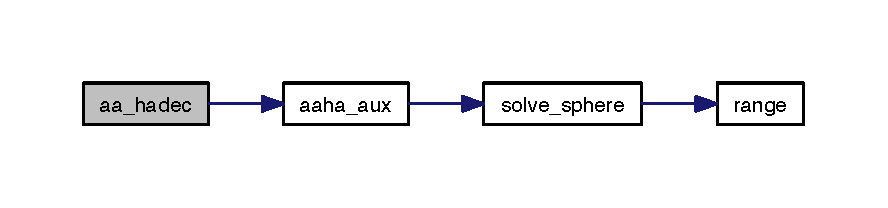
\includegraphics[width=350pt]{astro_8h_afb4e9b19dfbf97eaf03b05111e9e919d_cgraph}
\end{center}
\end{figure}




Here is the caller graph for this function\-:
\nopagebreak
\begin{figure}[H]
\begin{center}
\leavevmode
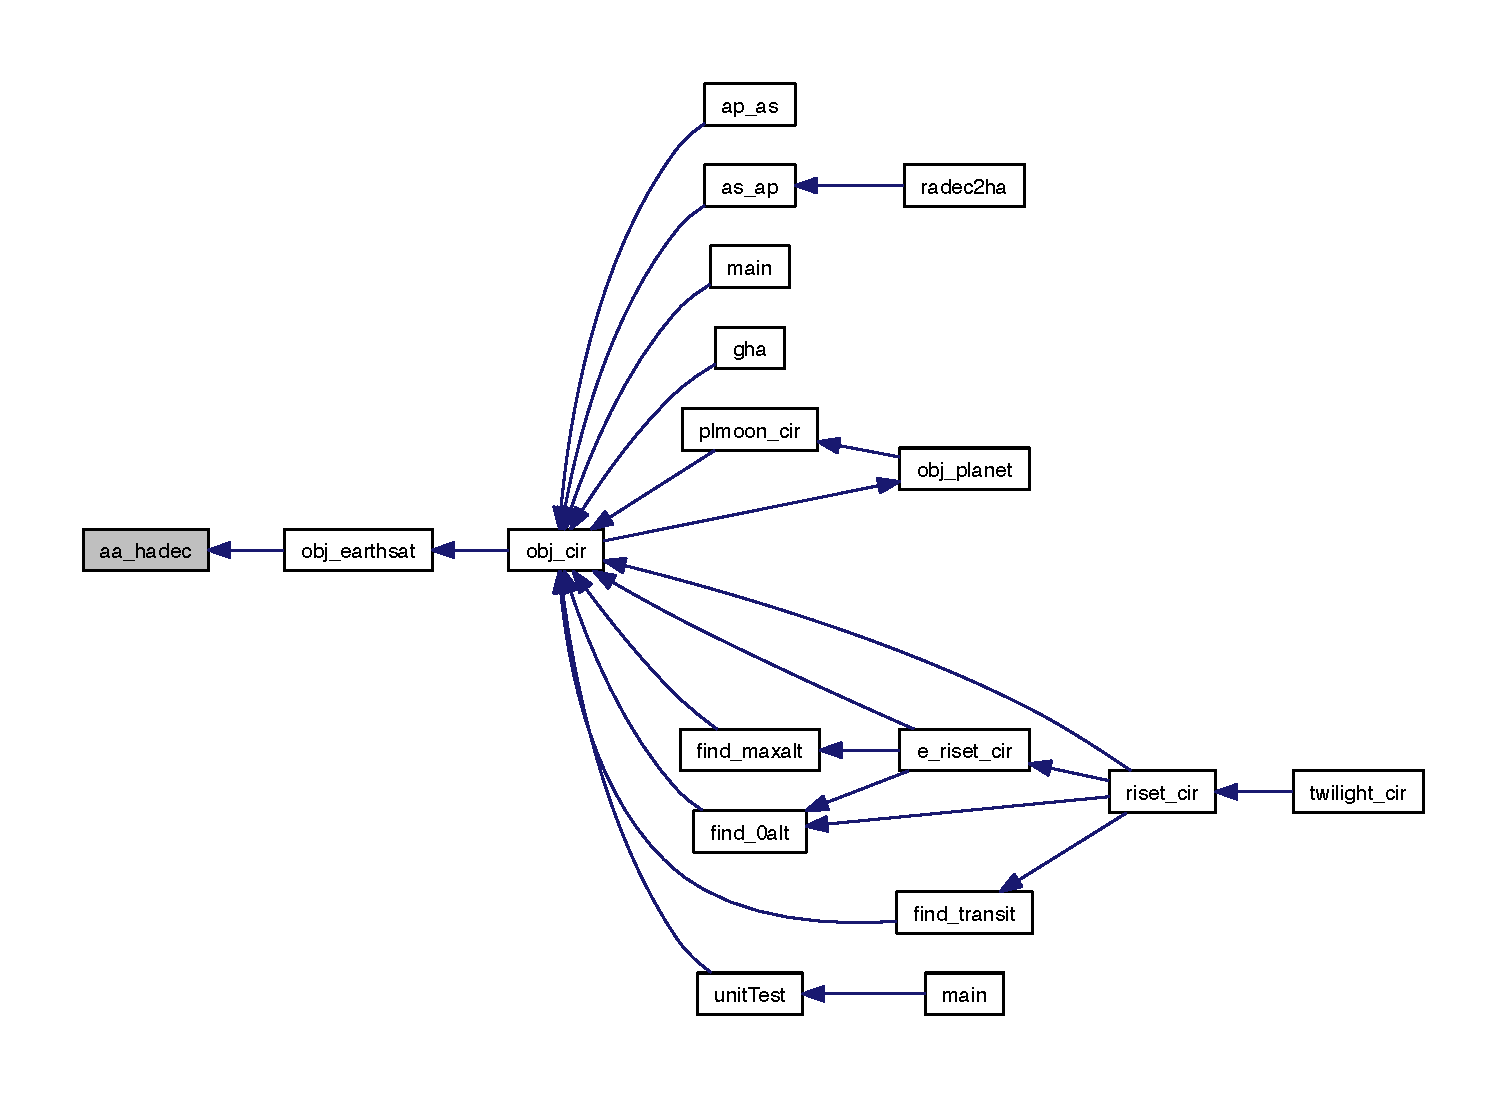
\includegraphics[width=350pt]{astro_8h_afb4e9b19dfbf97eaf03b05111e9e919d_icgraph}
\end{center}
\end{figure}


\hypertarget{astro_8h_abef08d899770c40423cbf24280ab10cf}{\index{astro.\-h@{astro.\-h}!ab\-\_\-ecl@{ab\-\_\-ecl}}
\index{ab\-\_\-ecl@{ab\-\_\-ecl}!astro.h@{astro.\-h}}
\subsubsection[{ab\-\_\-ecl}]{\setlength{\rightskip}{0pt plus 5cm}void ab\-\_\-ecl (
\begin{DoxyParamCaption}
\item[{double}]{m, }
\item[{double}]{lsn, }
\item[{double $\ast$}]{lam, }
\item[{double $\ast$}]{bet}
\end{DoxyParamCaption}
)}}\label{astro_8h_abef08d899770c40423cbf24280ab10cf}


Definition at line 25 of file aberration.\-c.



Here is the call graph for this function\-:
\nopagebreak
\begin{figure}[H]
\begin{center}
\leavevmode
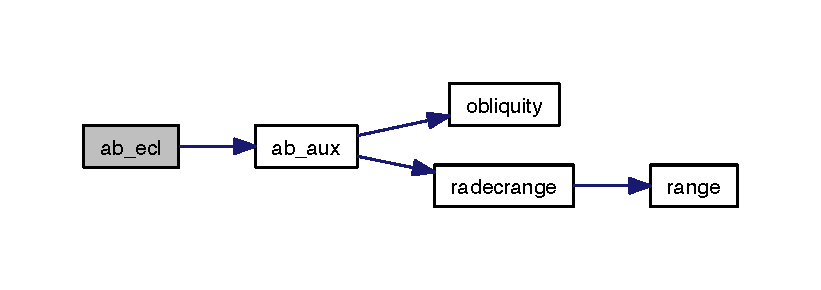
\includegraphics[width=350pt]{astro_8h_abef08d899770c40423cbf24280ab10cf_cgraph}
\end{center}
\end{figure}


\hypertarget{astro_8h_aee075aa543ef48c790c4b6b7c965db1b}{\index{astro.\-h@{astro.\-h}!ab\-\_\-eq@{ab\-\_\-eq}}
\index{ab\-\_\-eq@{ab\-\_\-eq}!astro.h@{astro.\-h}}
\subsubsection[{ab\-\_\-eq}]{\setlength{\rightskip}{0pt plus 5cm}void ab\-\_\-eq (
\begin{DoxyParamCaption}
\item[{double}]{m, }
\item[{double}]{lsn, }
\item[{double $\ast$}]{ra, }
\item[{double $\ast$}]{dec}
\end{DoxyParamCaption}
)}}\label{astro_8h_aee075aa543ef48c790c4b6b7c965db1b}


Definition at line 35 of file aberration.\-c.



Here is the call graph for this function\-:
\nopagebreak
\begin{figure}[H]
\begin{center}
\leavevmode
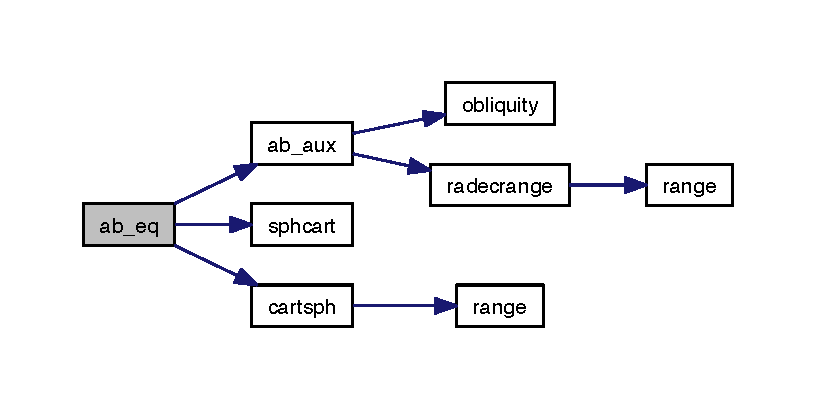
\includegraphics[width=350pt]{astro_8h_aee075aa543ef48c790c4b6b7c965db1b_cgraph}
\end{center}
\end{figure}




Here is the caller graph for this function\-:
\nopagebreak
\begin{figure}[H]
\begin{center}
\leavevmode
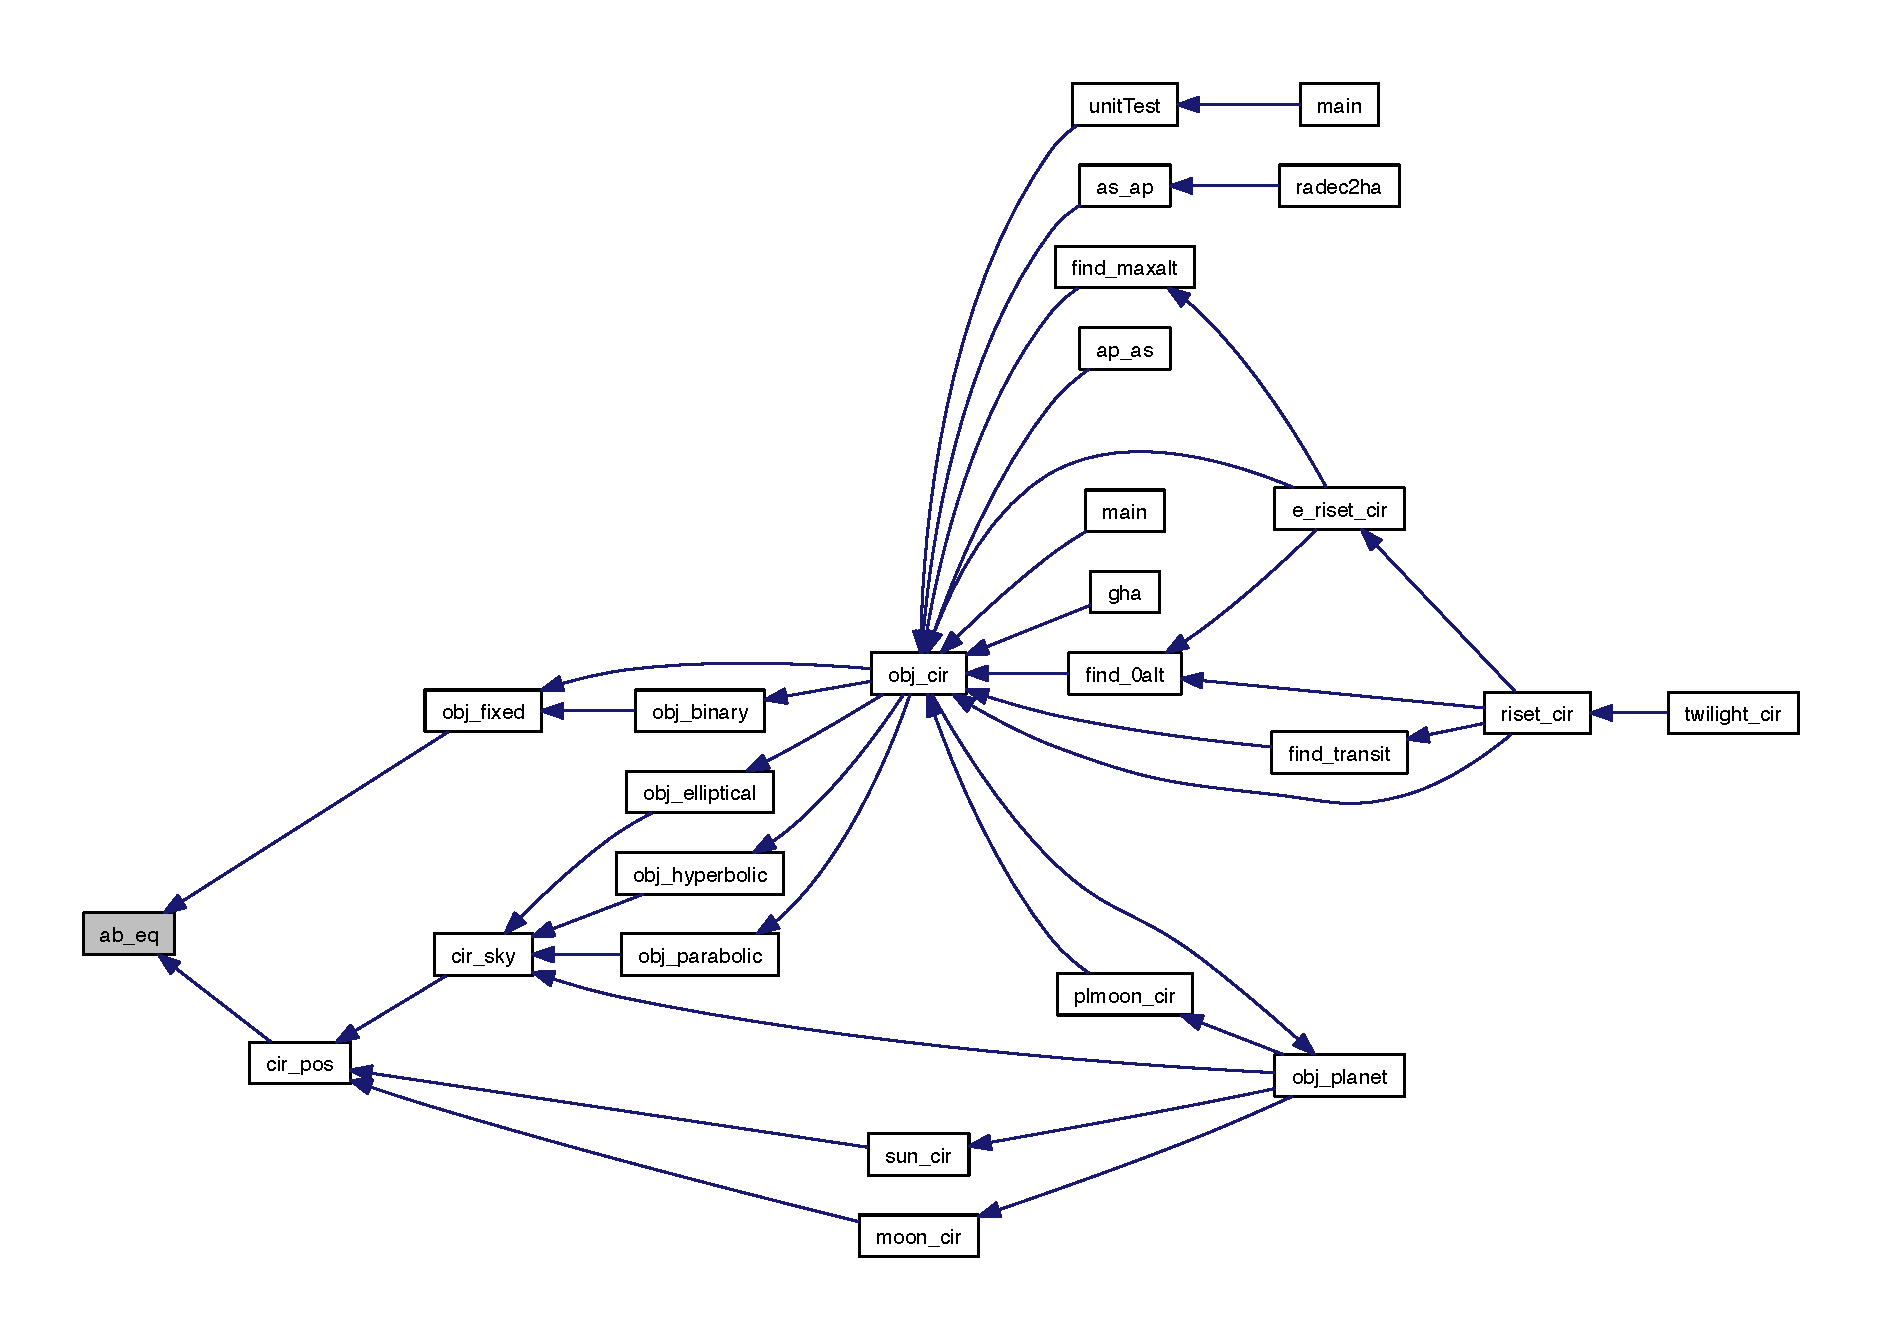
\includegraphics[width=350pt]{astro_8h_aee075aa543ef48c790c4b6b7c965db1b_icgraph}
\end{center}
\end{figure}


\hypertarget{astro_8h_a0149c681dca5872a5194adc30048833e}{\index{astro.\-h@{astro.\-h}!airmass@{airmass}}
\index{airmass@{airmass}!astro.h@{astro.\-h}}
\subsubsection[{airmass}]{\setlength{\rightskip}{0pt plus 5cm}void airmass (
\begin{DoxyParamCaption}
\item[{double}]{aa, }
\item[{double $\ast$}]{Xp}
\end{DoxyParamCaption}
)}}\label{astro_8h_a0149c681dca5872a5194adc30048833e}


Definition at line 11 of file airmass.\-c.

\hypertarget{astro_8h_ab35408588a03873bb6cfc73b8b7aa349}{\index{astro.\-h@{astro.\-h}!anomaly@{anomaly}}
\index{anomaly@{anomaly}!astro.h@{astro.\-h}}
\subsubsection[{anomaly}]{\setlength{\rightskip}{0pt plus 5cm}void anomaly (
\begin{DoxyParamCaption}
\item[{double}]{ma, }
\item[{double}]{s, }
\item[{double $\ast$}]{nu, }
\item[{double $\ast$}]{ea}
\end{DoxyParamCaption}
)}}\label{astro_8h_ab35408588a03873bb6cfc73b8b7aa349}


Definition at line 17 of file anomaly.\-c.



Here is the call graph for this function\-:
\nopagebreak
\begin{figure}[H]
\begin{center}
\leavevmode
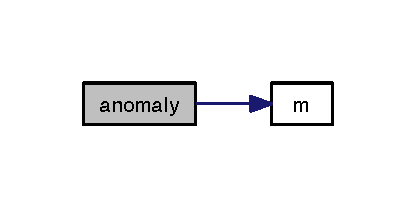
\includegraphics[width=200pt]{astro_8h_ab35408588a03873bb6cfc73b8b7aa349_cgraph}
\end{center}
\end{figure}




Here is the caller graph for this function\-:
\nopagebreak
\begin{figure}[H]
\begin{center}
\leavevmode
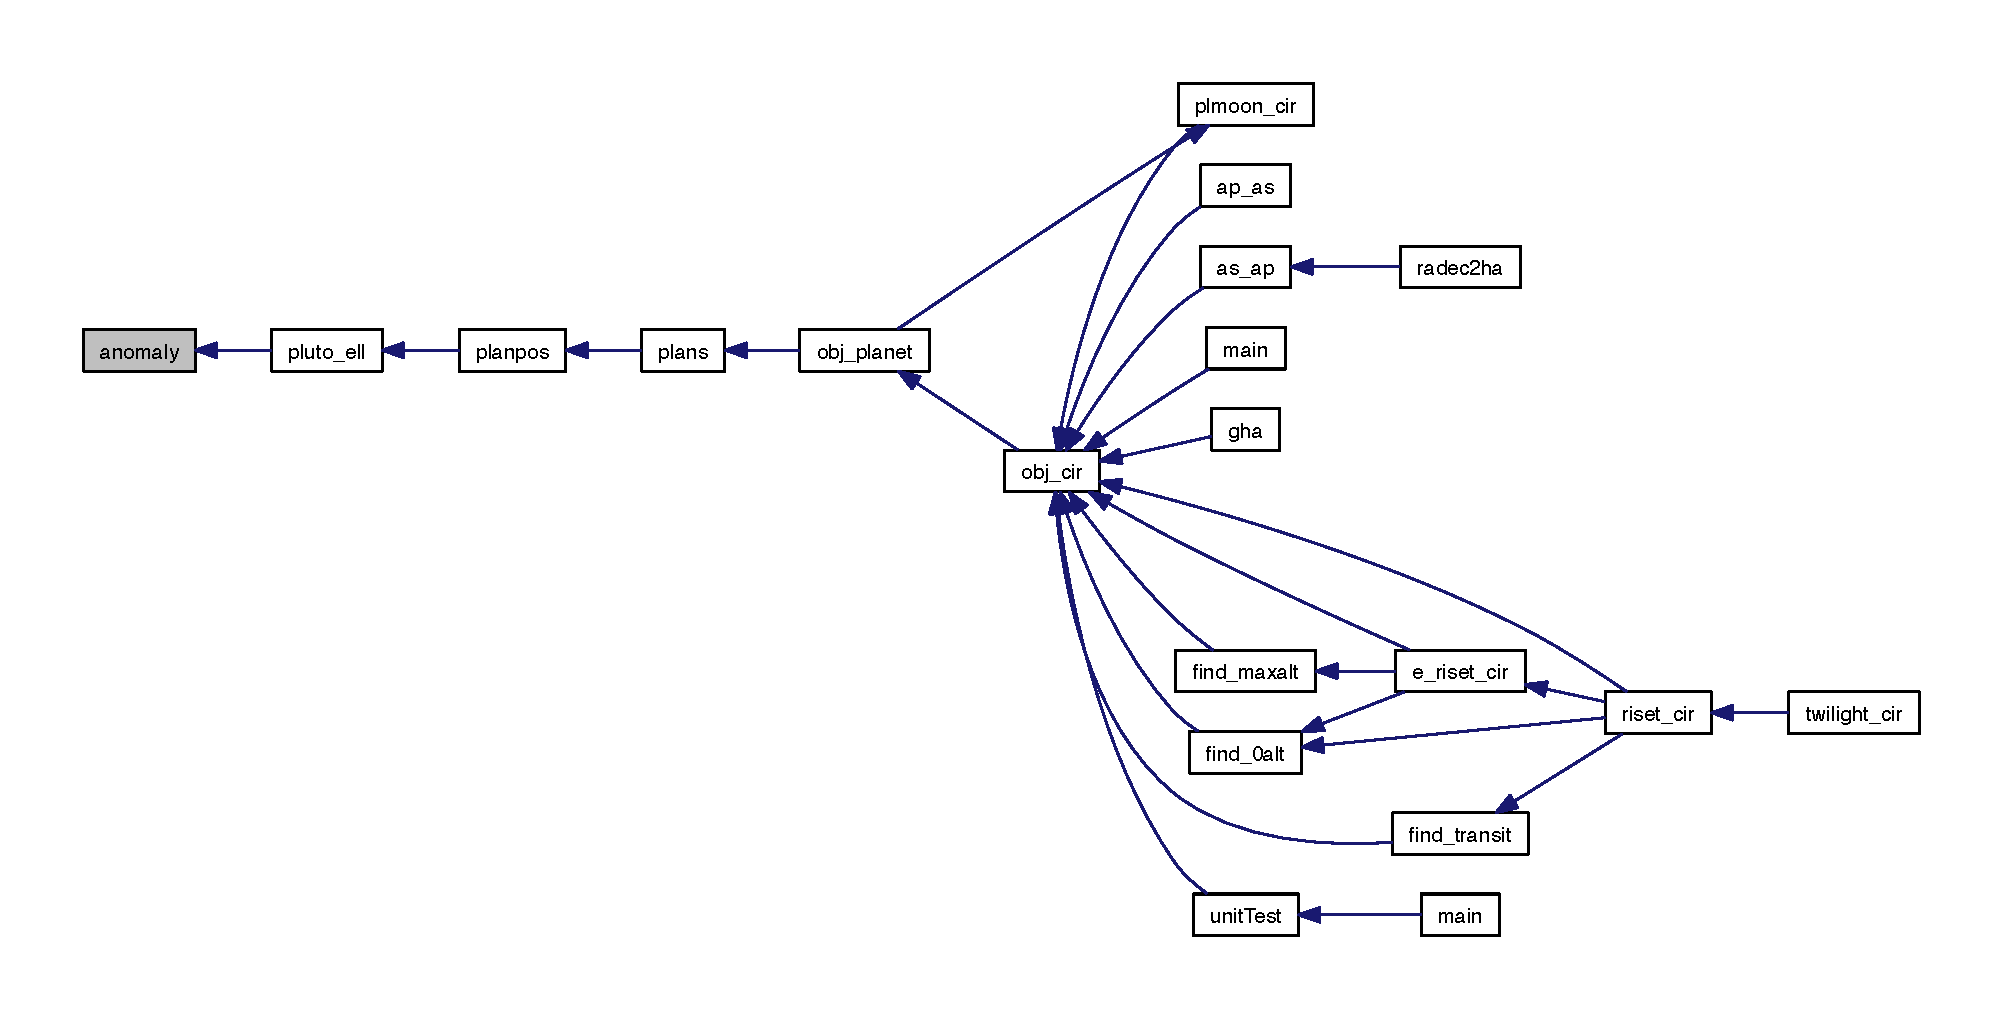
\includegraphics[width=350pt]{astro_8h_ab35408588a03873bb6cfc73b8b7aa349_icgraph}
\end{center}
\end{figure}


\hypertarget{astro_8h_a11919b10760f866b904d4d154eede26e}{\index{astro.\-h@{astro.\-h}!ap\-\_\-as@{ap\-\_\-as}}
\index{ap\-\_\-as@{ap\-\_\-as}!astro.h@{astro.\-h}}
\subsubsection[{ap\-\_\-as}]{\setlength{\rightskip}{0pt plus 5cm}void ap\-\_\-as (
\begin{DoxyParamCaption}
\item[{{\bf Now} $\ast$}]{np, }
\item[{double}]{Mjd, }
\item[{double $\ast$}]{rap, }
\item[{double $\ast$}]{decp}
\end{DoxyParamCaption}
)}}\label{astro_8h_a11919b10760f866b904d4d154eede26e}


Definition at line 12 of file ap\-\_\-as.\-c.



Here is the call graph for this function\-:
\nopagebreak
\begin{figure}[H]
\begin{center}
\leavevmode
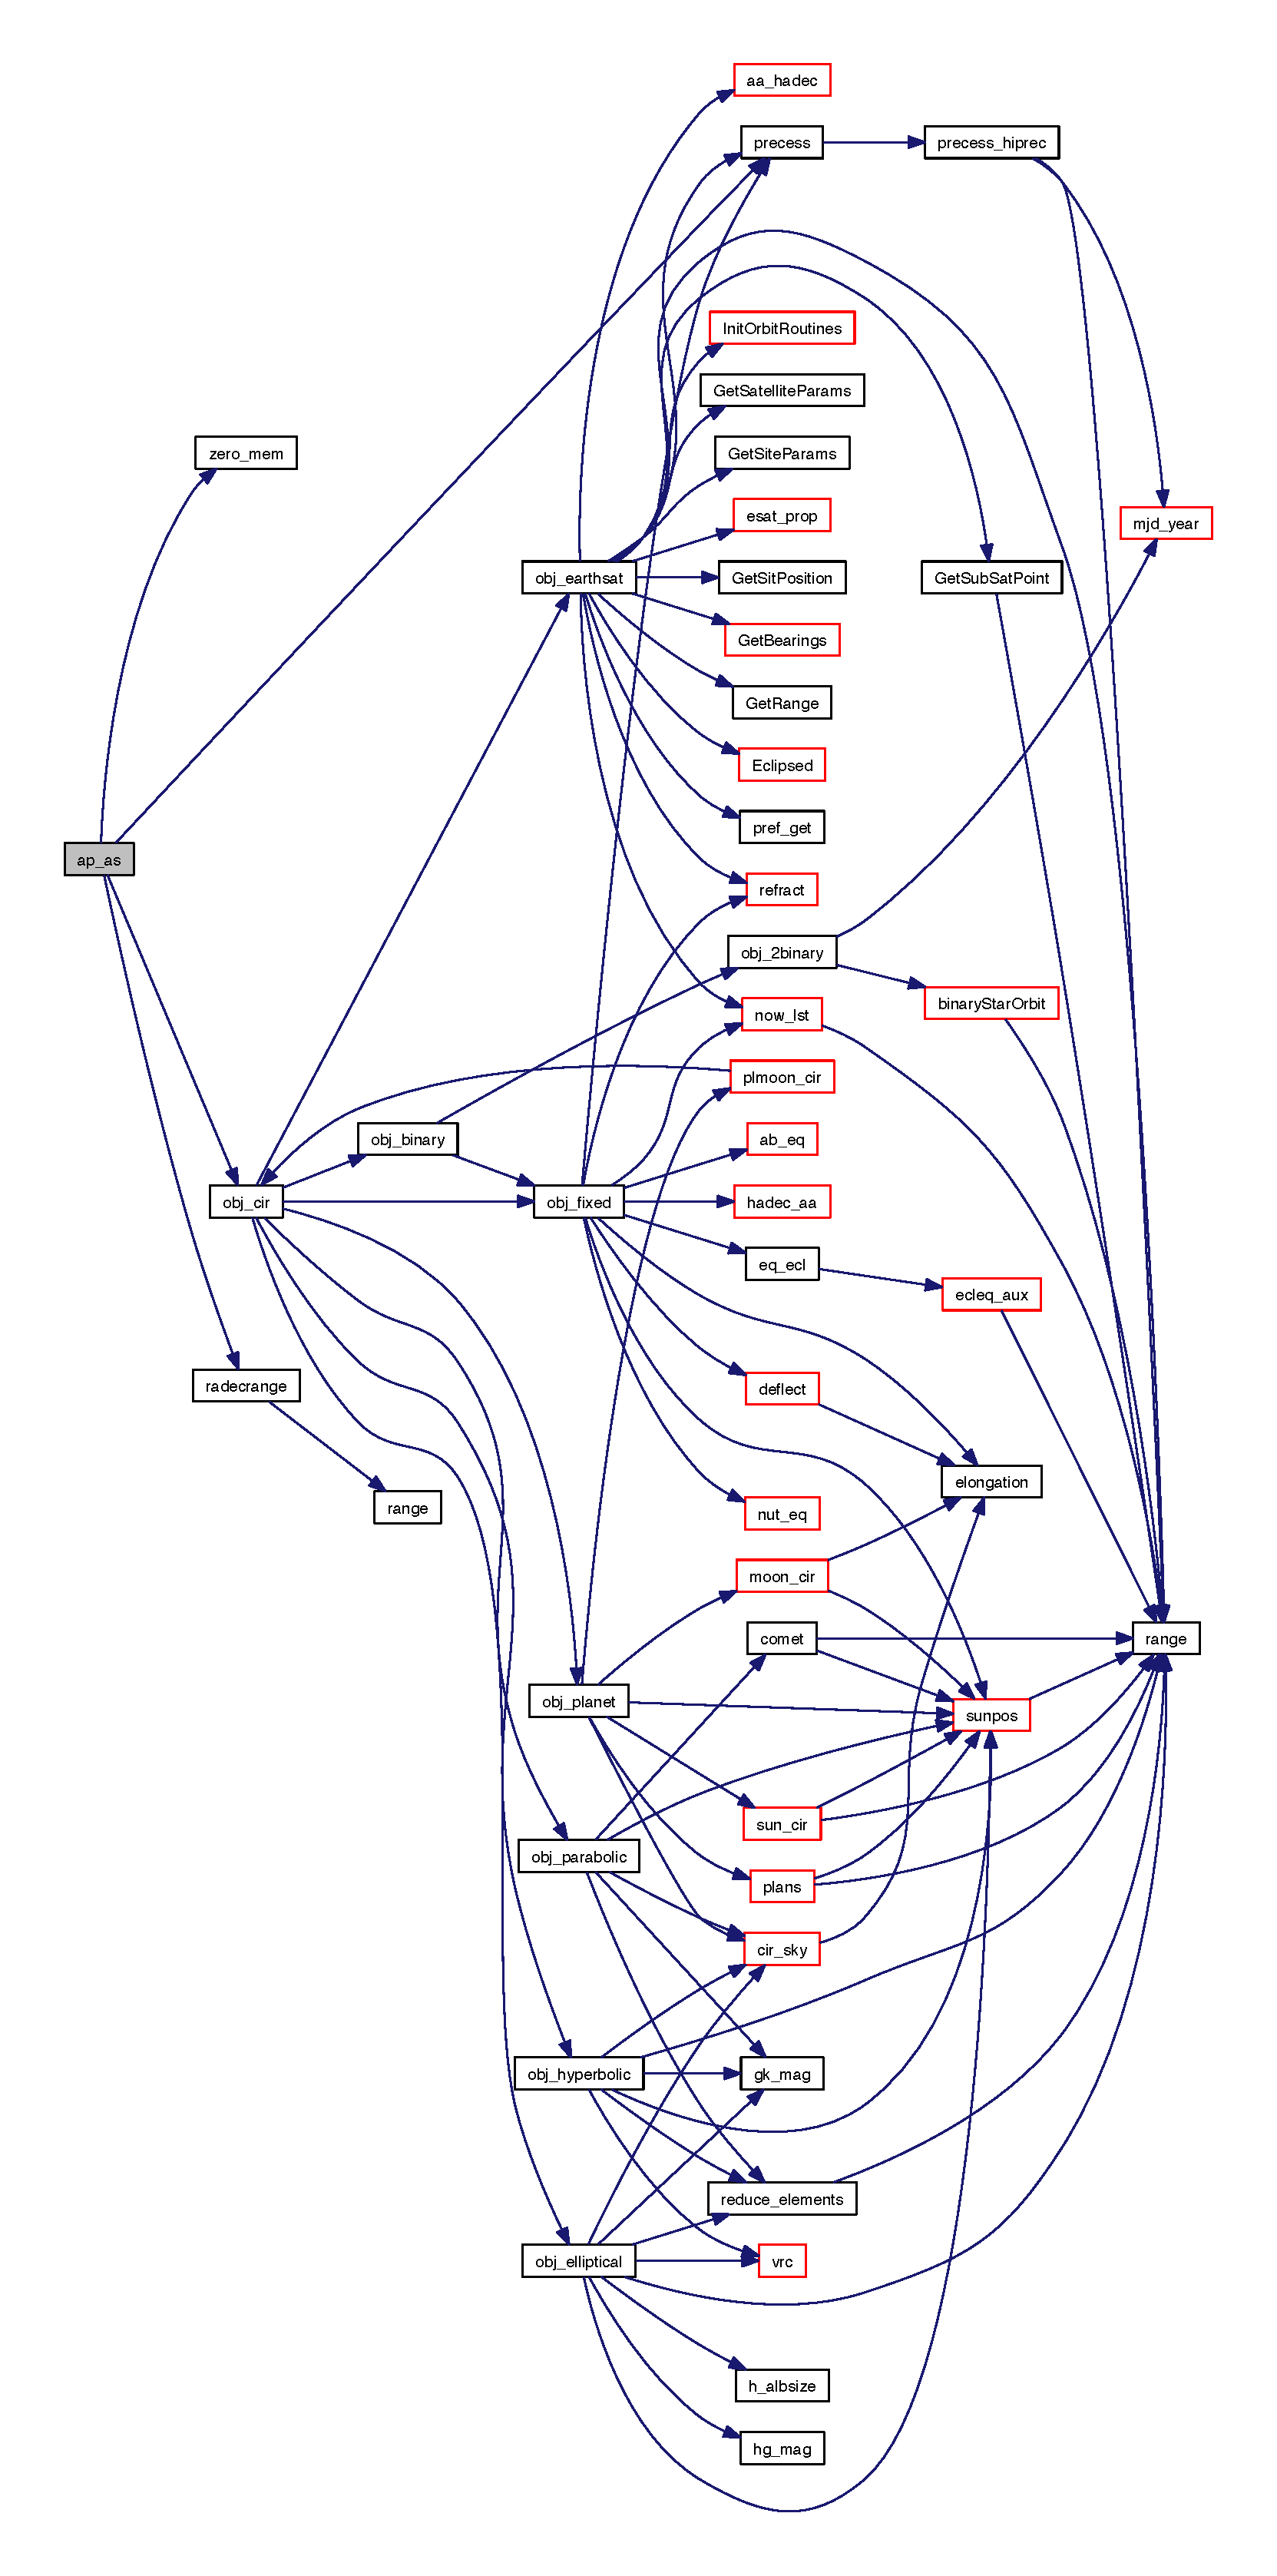
\includegraphics[height=550pt]{astro_8h_a11919b10760f866b904d4d154eede26e_cgraph}
\end{center}
\end{figure}


\hypertarget{astro_8h_a7aca2af85728e9b6336700b2753c6790}{\index{astro.\-h@{astro.\-h}!as\-\_\-ap@{as\-\_\-ap}}
\index{as\-\_\-ap@{as\-\_\-ap}!astro.h@{astro.\-h}}
\subsubsection[{as\-\_\-ap}]{\setlength{\rightskip}{0pt plus 5cm}void as\-\_\-ap (
\begin{DoxyParamCaption}
\item[{{\bf Now} $\ast$}]{np, }
\item[{double}]{Mjd, }
\item[{double $\ast$}]{rap, }
\item[{double $\ast$}]{decp}
\end{DoxyParamCaption}
)}}\label{astro_8h_a7aca2af85728e9b6336700b2753c6790}


Definition at line 50 of file ap\-\_\-as.\-c.



Here is the call graph for this function\-:
\nopagebreak
\begin{figure}[H]
\begin{center}
\leavevmode
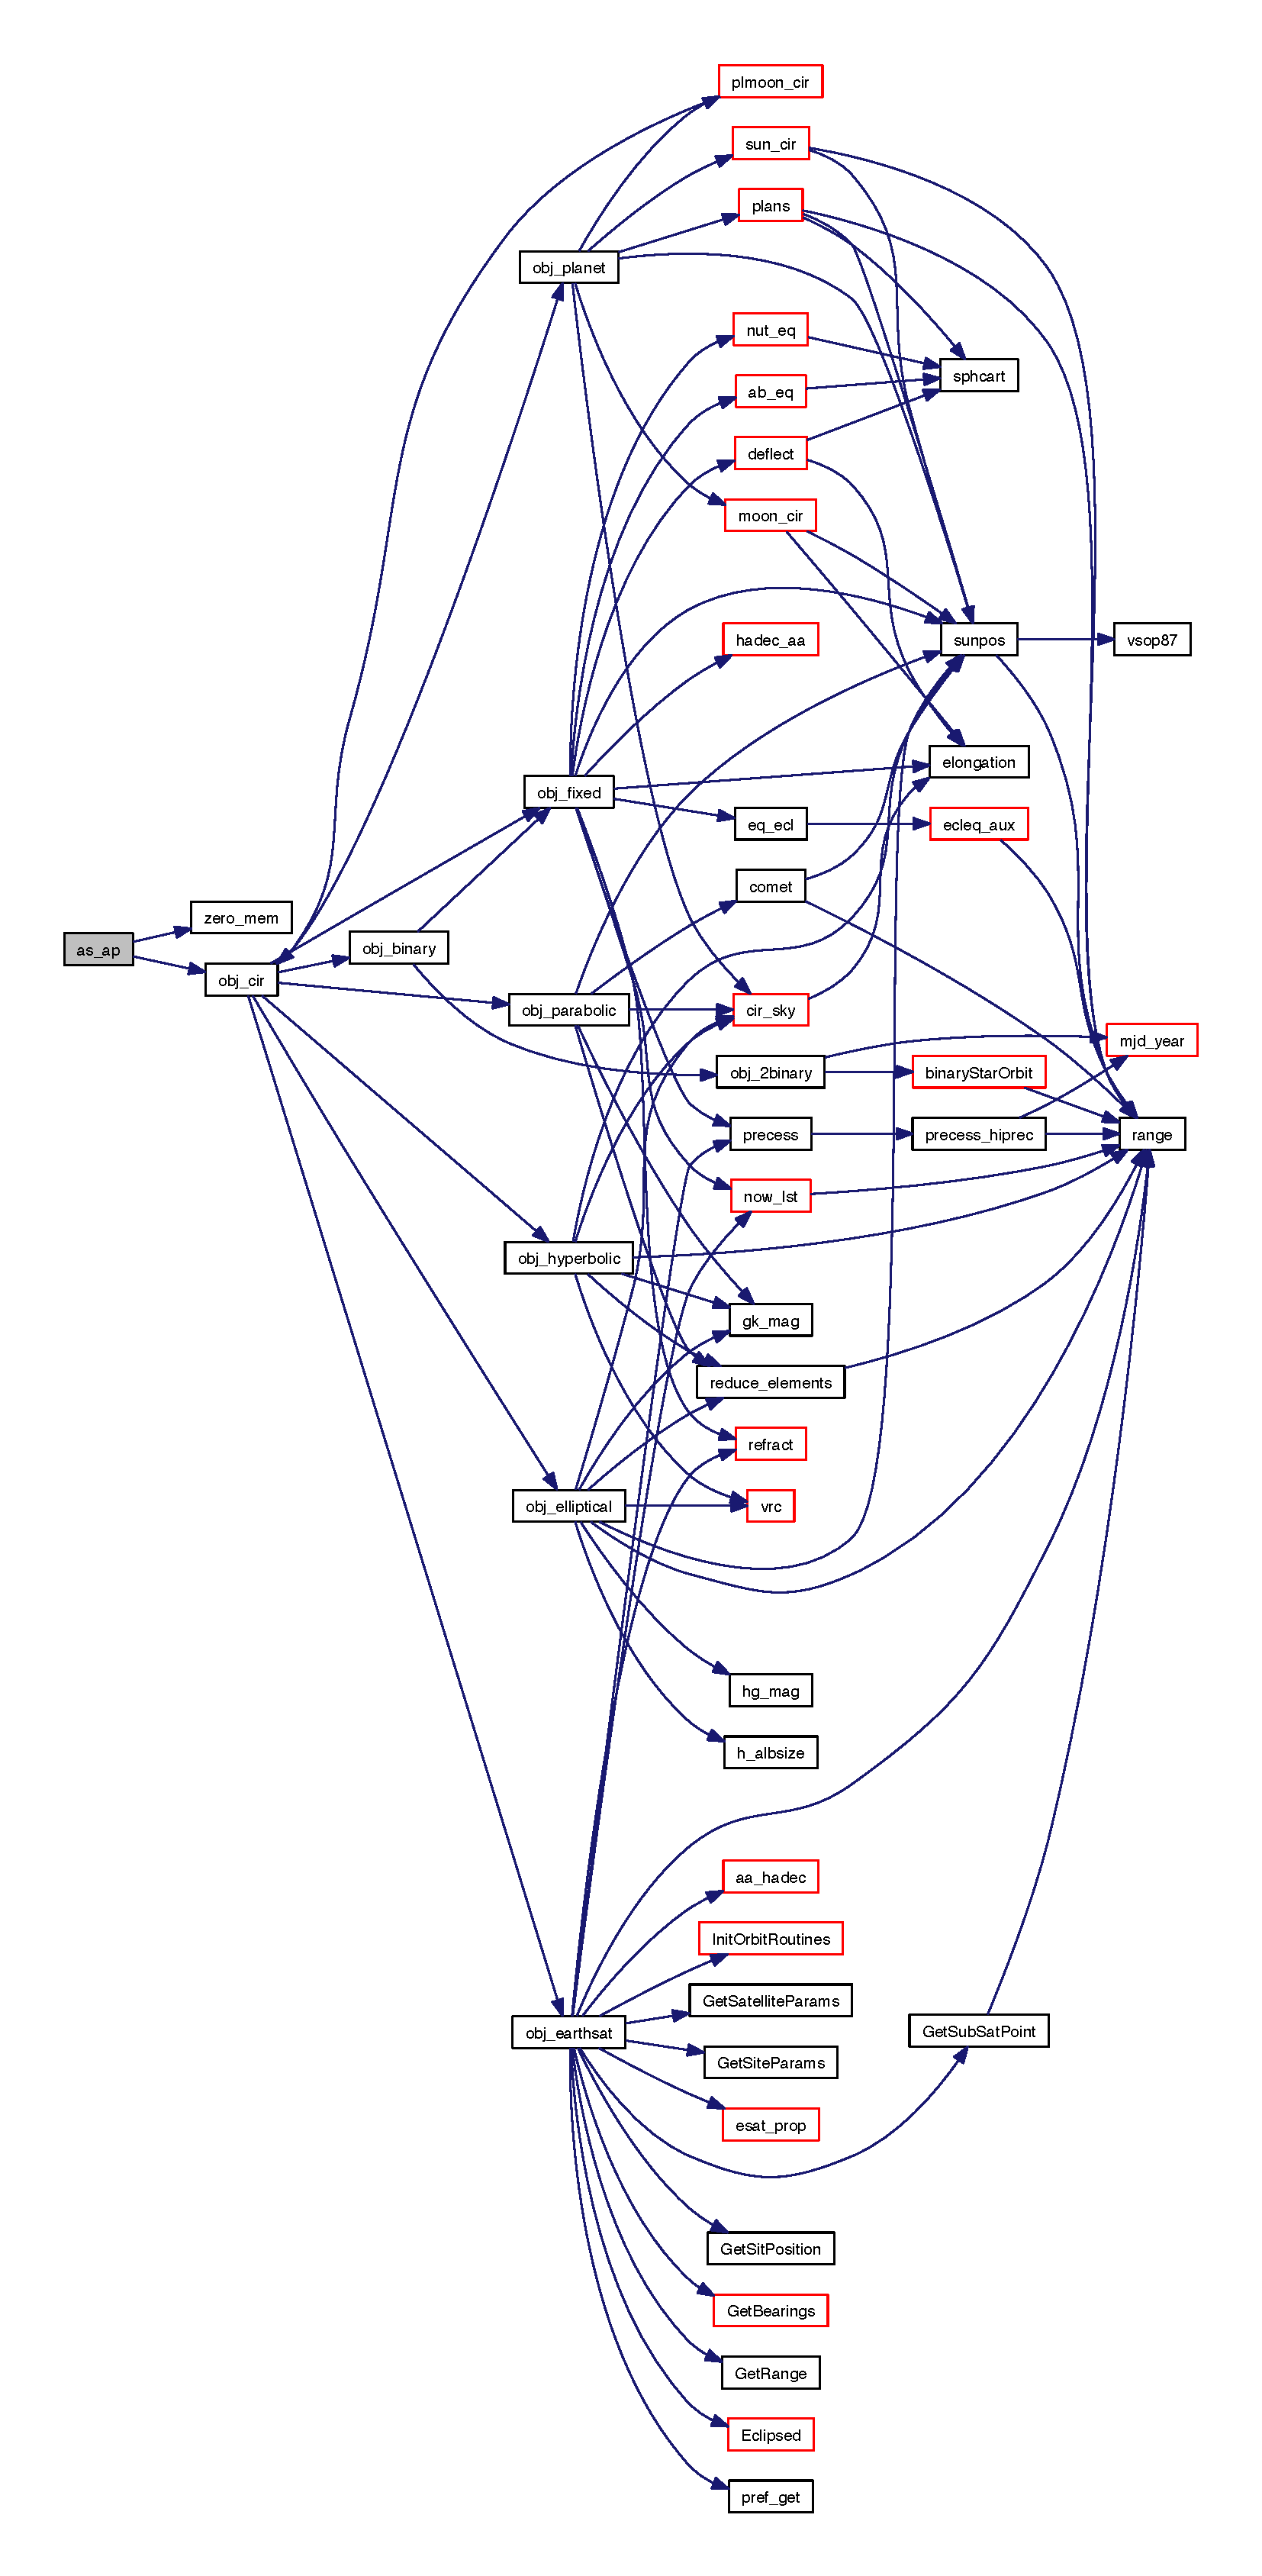
\includegraphics[height=550pt]{astro_8h_a7aca2af85728e9b6336700b2753c6790_cgraph}
\end{center}
\end{figure}




Here is the caller graph for this function\-:
\nopagebreak
\begin{figure}[H]
\begin{center}
\leavevmode
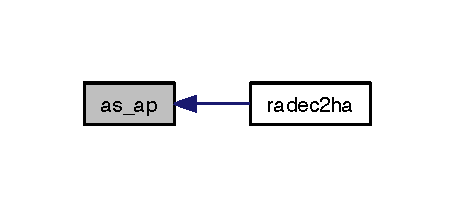
\includegraphics[width=218pt]{astro_8h_a7aca2af85728e9b6336700b2753c6790_icgraph}
\end{center}
\end{figure}


\hypertarget{astro_8h_aa6d912aad096356910df21a7371278b6}{\index{astro.\-h@{astro.\-h}!atod@{atod}}
\index{atod@{atod}!astro.h@{astro.\-h}}
\subsubsection[{atod}]{\setlength{\rightskip}{0pt plus 5cm}double atod (
\begin{DoxyParamCaption}
\item[{char $\ast$}]{buf}
\end{DoxyParamCaption}
)}}\label{astro_8h_aa6d912aad096356910df21a7371278b6}


Definition at line 357 of file misc.\-c.



Here is the caller graph for this function\-:
\nopagebreak
\begin{figure}[H]
\begin{center}
\leavevmode
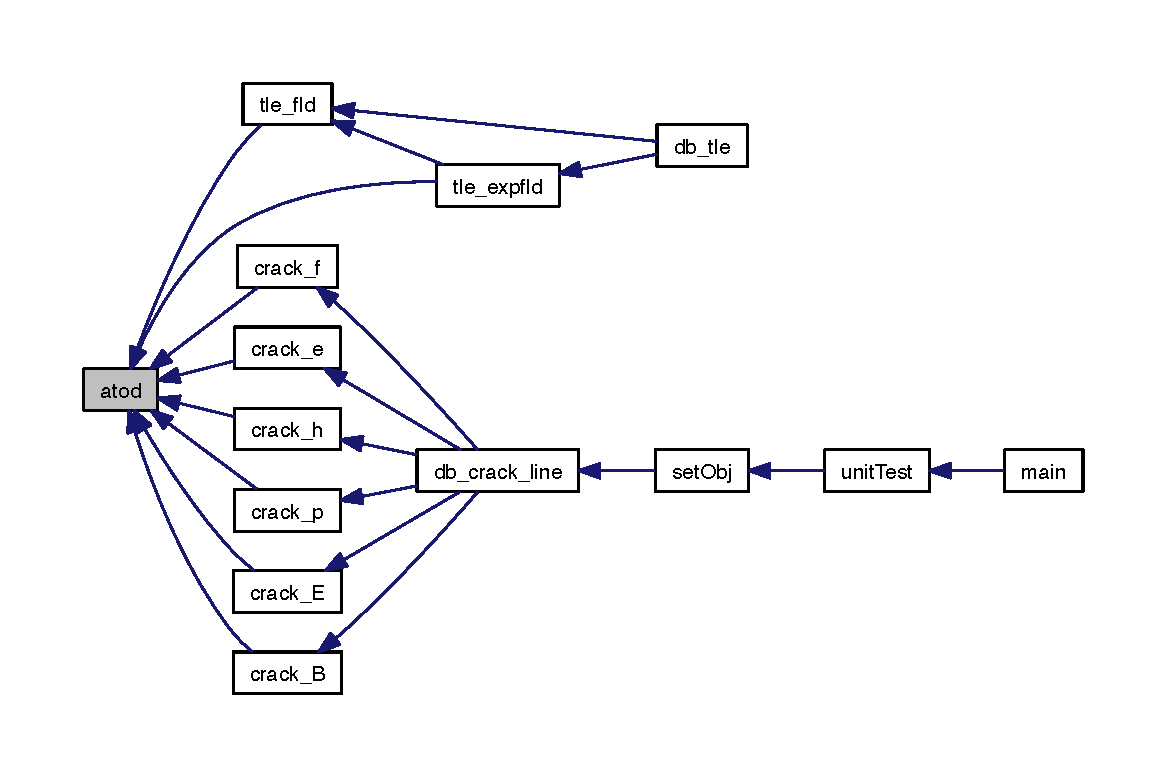
\includegraphics[width=350pt]{astro_8h_aa6d912aad096356910df21a7371278b6_icgraph}
\end{center}
\end{figure}


\hypertarget{astro_8h_adfefefa5bc6c1d3a4d06cc4a88608dac}{\index{astro.\-h@{astro.\-h}!cal\-\_\-mjd@{cal\-\_\-mjd}}
\index{cal\-\_\-mjd@{cal\-\_\-mjd}!astro.h@{astro.\-h}}
\subsubsection[{cal\-\_\-mjd}]{\setlength{\rightskip}{0pt plus 5cm}void cal\-\_\-mjd (
\begin{DoxyParamCaption}
\item[{int}]{mn, }
\item[{double}]{dy, }
\item[{int}]{yr, }
\item[{double $\ast$}]{m}
\end{DoxyParamCaption}
)}}\label{astro_8h_adfefefa5bc6c1d3a4d06cc4a88608dac}


Definition at line 13 of file mjd.\-c.



Here is the call graph for this function\-:
\nopagebreak
\begin{figure}[H]
\begin{center}
\leavevmode
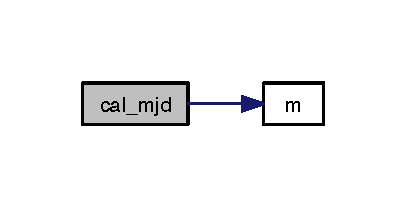
\includegraphics[width=196pt]{astro_8h_adfefefa5bc6c1d3a4d06cc4a88608dac_cgraph}
\end{center}
\end{figure}




Here is the caller graph for this function\-:
\nopagebreak
\begin{figure}[H]
\begin{center}
\leavevmode
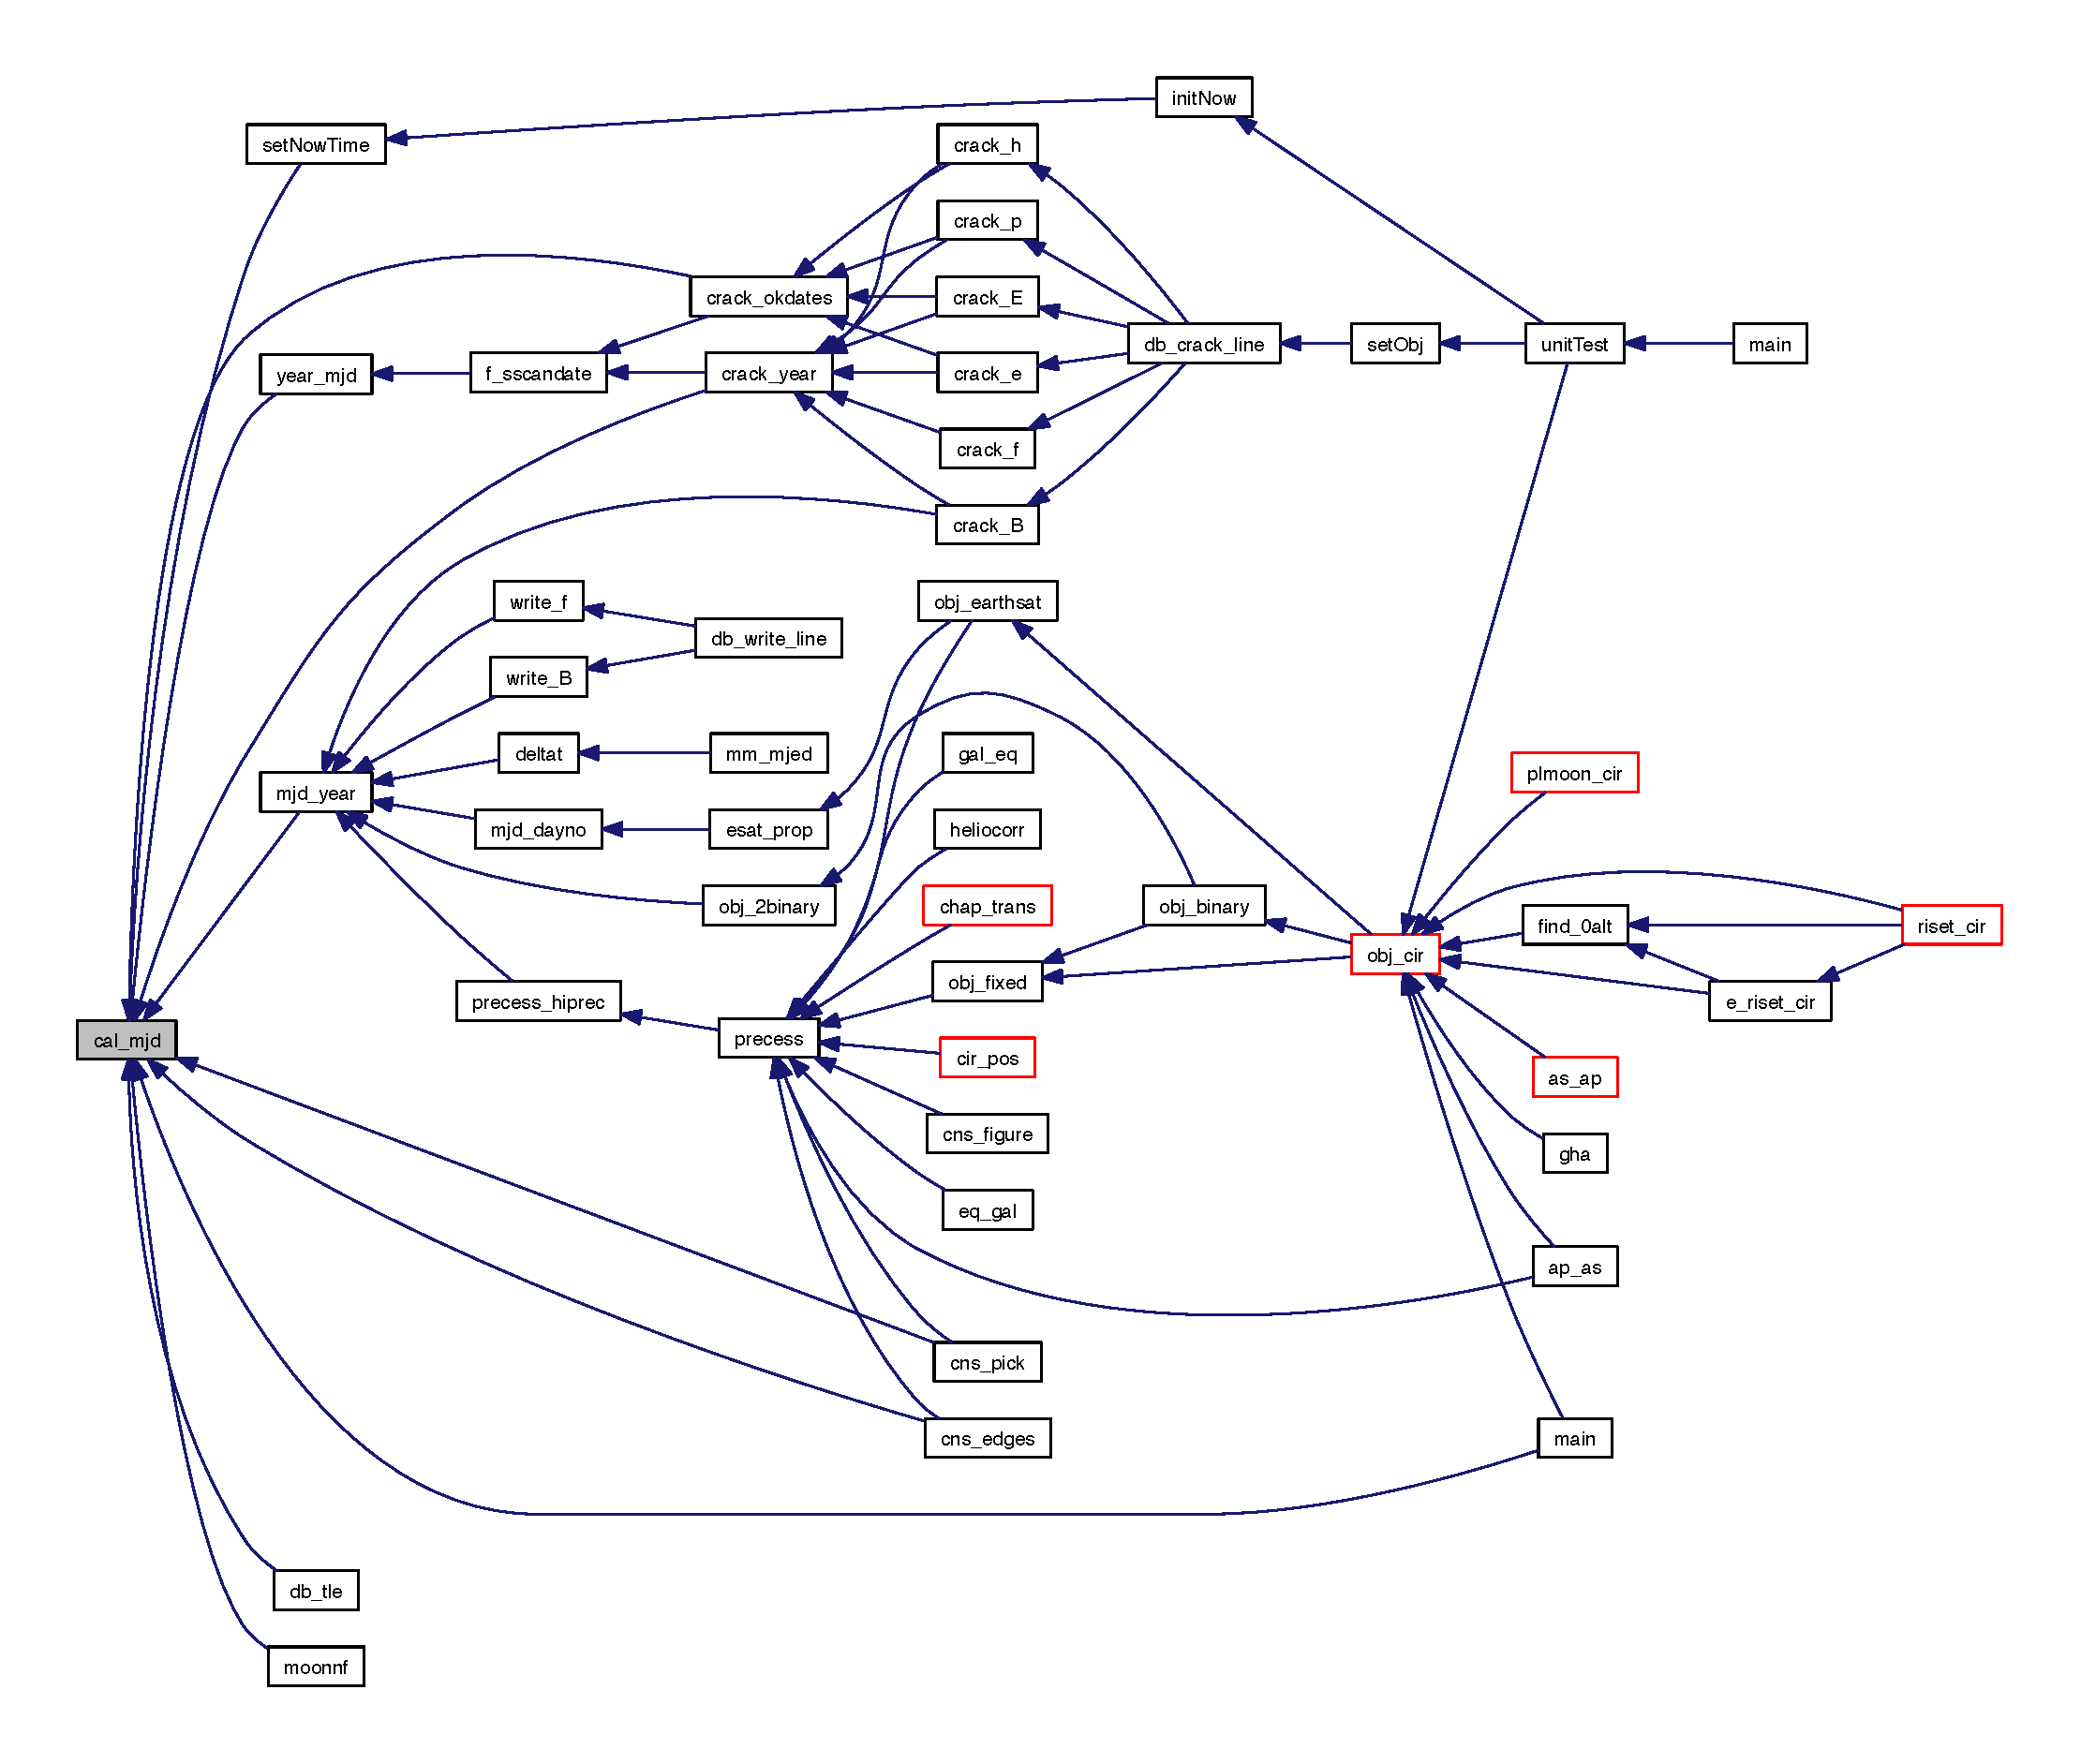
\includegraphics[width=350pt]{astro_8h_adfefefa5bc6c1d3a4d06cc4a88608dac_icgraph}
\end{center}
\end{figure}


\hypertarget{astro_8h_a3deb7d78e5b24bcab18d469cdbc7bcc2}{\index{astro.\-h@{astro.\-h}!cartsph@{cartsph}}
\index{cartsph@{cartsph}!astro.h@{astro.\-h}}
\subsubsection[{cartsph}]{\setlength{\rightskip}{0pt plus 5cm}void cartsph (
\begin{DoxyParamCaption}
\item[{double}]{x, }
\item[{double}]{y, }
\item[{double}]{z, }
\item[{double $\ast$}]{l, }
\item[{double $\ast$}]{b, }
\item[{double $\ast$}]{r}
\end{DoxyParamCaption}
)}}\label{astro_8h_a3deb7d78e5b24bcab18d469cdbc7bcc2}


Definition at line 21 of file sphcart.\-c.



Here is the call graph for this function\-:
\nopagebreak
\begin{figure}[H]
\begin{center}
\leavevmode
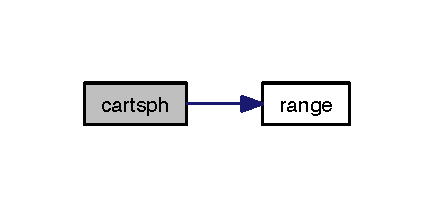
\includegraphics[width=208pt]{astro_8h_a3deb7d78e5b24bcab18d469cdbc7bcc2_cgraph}
\end{center}
\end{figure}




Here is the caller graph for this function\-:
\nopagebreak
\begin{figure}[H]
\begin{center}
\leavevmode
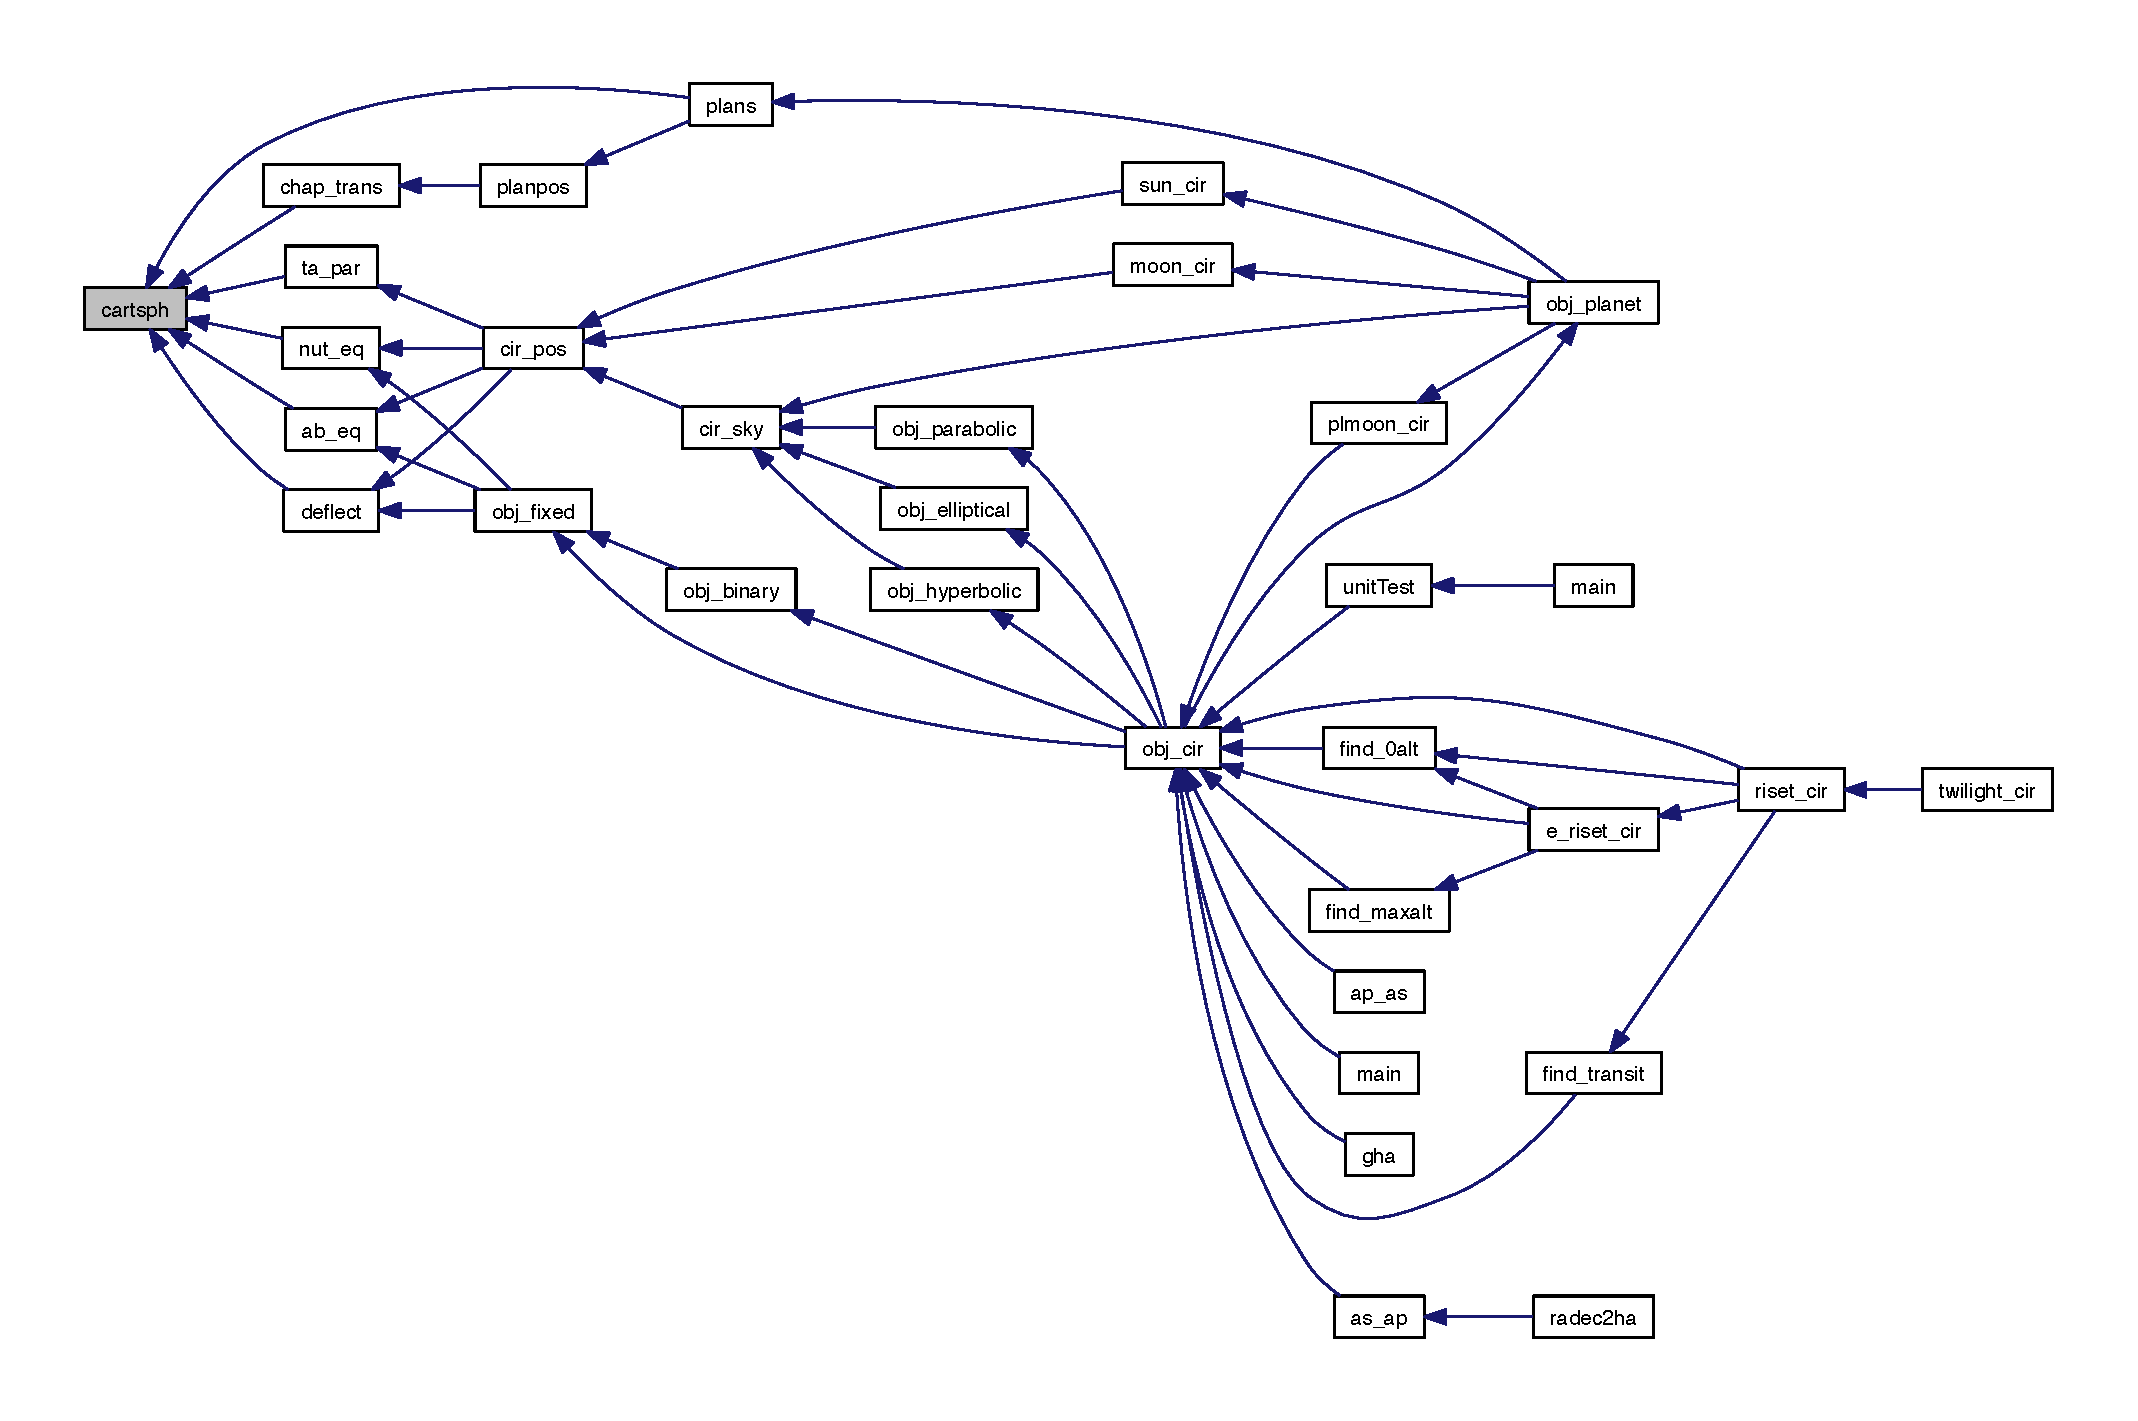
\includegraphics[width=350pt]{astro_8h_a3deb7d78e5b24bcab18d469cdbc7bcc2_icgraph}
\end{center}
\end{figure}


\hypertarget{astro_8h_a3c04fc909e750cb1784cadf3101bddcc}{\index{astro.\-h@{astro.\-h}!chap95@{chap95}}
\index{chap95@{chap95}!astro.h@{astro.\-h}}
\subsubsection[{chap95}]{\setlength{\rightskip}{0pt plus 5cm}int chap95 (
\begin{DoxyParamCaption}
\item[{double}]{m, }
\item[{int}]{obj, }
\item[{double}]{prec, }
\item[{double $\ast$}]{ret}
\end{DoxyParamCaption}
)}}\label{astro_8h_a3c04fc909e750cb1784cadf3101bddcc}


Definition at line 50 of file chap95.\-c.



Here is the caller graph for this function\-:
\nopagebreak
\begin{figure}[H]
\begin{center}
\leavevmode
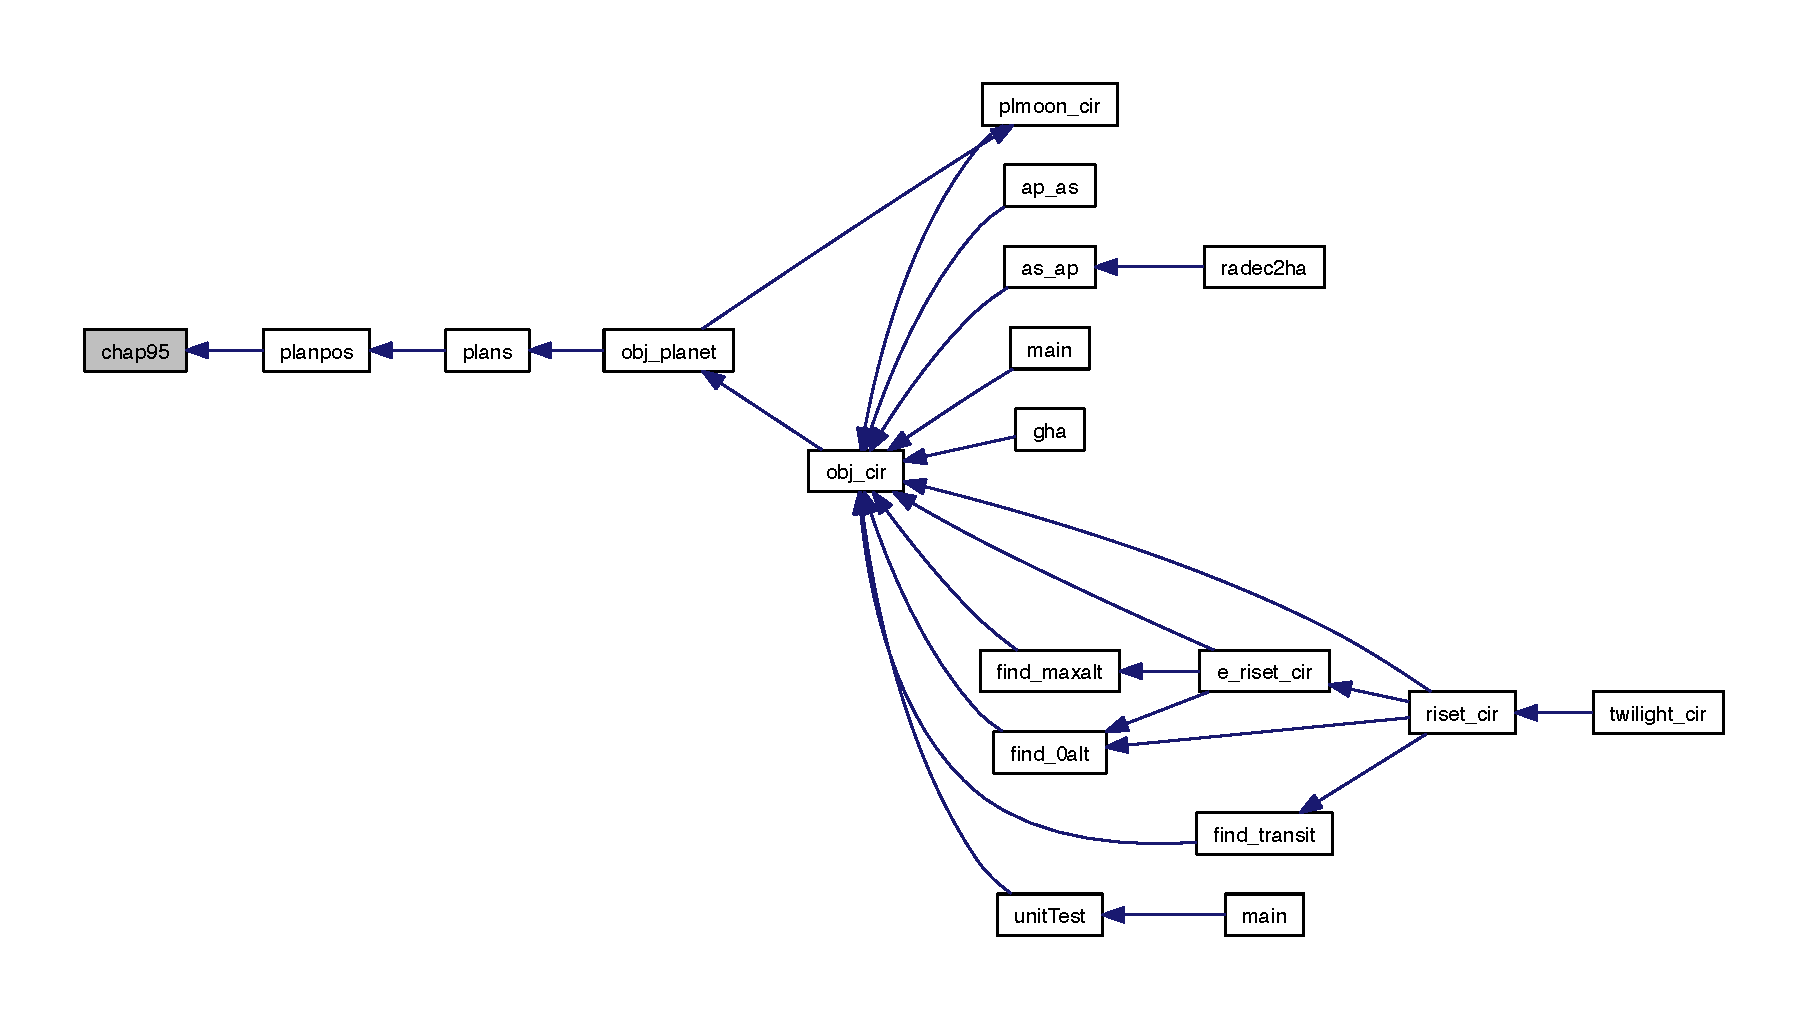
\includegraphics[width=350pt]{astro_8h_a3c04fc909e750cb1784cadf3101bddcc_icgraph}
\end{center}
\end{figure}


\hypertarget{astro_8h_a03e1b115ca90718115d025bc167ce6a8}{\index{astro.\-h@{astro.\-h}!cns\-\_\-edges@{cns\-\_\-edges}}
\index{cns\-\_\-edges@{cns\-\_\-edges}!astro.h@{astro.\-h}}
\subsubsection[{cns\-\_\-edges}]{\setlength{\rightskip}{0pt plus 5cm}int cns\-\_\-edges (
\begin{DoxyParamCaption}
\item[{double}]{e, }
\item[{double $\ast$$\ast$}]{ra0p, }
\item[{double $\ast$$\ast$}]{dec0p, }
\item[{double $\ast$$\ast$}]{ra1p, }
\item[{double $\ast$$\ast$}]{dec1p}
\end{DoxyParamCaption}
)}}\label{astro_8h_a03e1b115ca90718115d025bc167ce6a8}


Definition at line 1519 of file constel.\-c.



Here is the call graph for this function\-:
\nopagebreak
\begin{figure}[H]
\begin{center}
\leavevmode
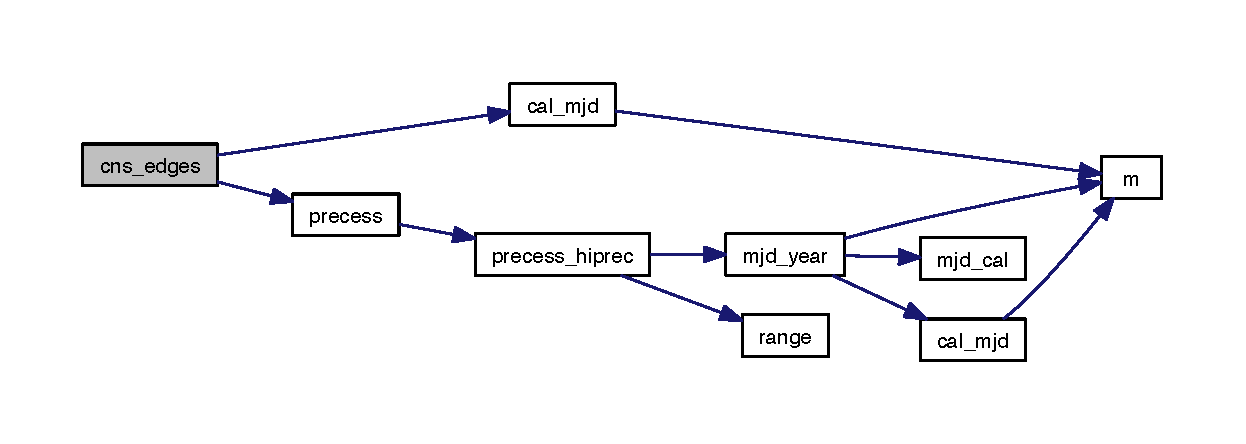
\includegraphics[width=350pt]{astro_8h_a03e1b115ca90718115d025bc167ce6a8_cgraph}
\end{center}
\end{figure}


\hypertarget{astro_8h_aa8601bb074905861837ddfda3f2bf0b1}{\index{astro.\-h@{astro.\-h}!cns\-\_\-figure@{cns\-\_\-figure}}
\index{cns\-\_\-figure@{cns\-\_\-figure}!astro.h@{astro.\-h}}
\subsubsection[{cns\-\_\-figure}]{\setlength{\rightskip}{0pt plus 5cm}int cns\-\_\-figure (
\begin{DoxyParamCaption}
\item[{int}]{id, }
\item[{double}]{e, }
\item[{double}]{ra\mbox{[}$\,$\mbox{]}, }
\item[{double}]{dec\mbox{[}$\,$\mbox{]}, }
\item[{int}]{dcodes\mbox{[}$\,$\mbox{]}}
\end{DoxyParamCaption}
)}}\label{astro_8h_aa8601bb074905861837ddfda3f2bf0b1}


Definition at line 1783 of file constel.\-c.



Here is the call graph for this function\-:
\nopagebreak
\begin{figure}[H]
\begin{center}
\leavevmode
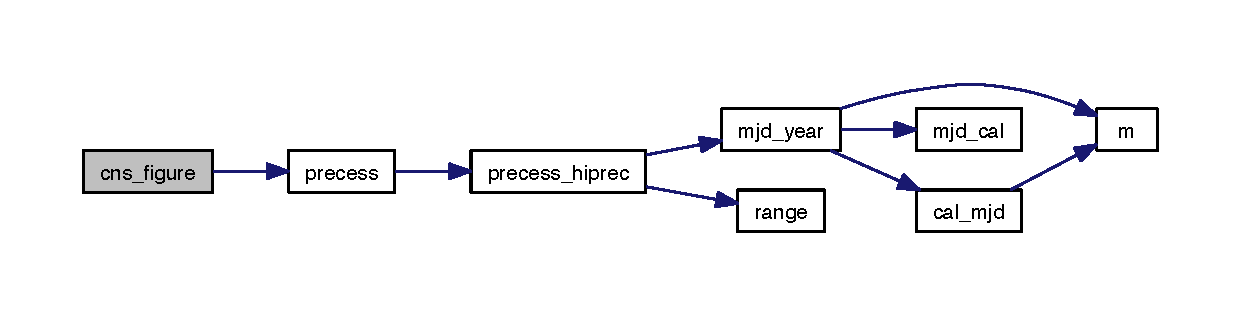
\includegraphics[width=350pt]{astro_8h_aa8601bb074905861837ddfda3f2bf0b1_cgraph}
\end{center}
\end{figure}


\hypertarget{astro_8h_a2fa52e582fb3bc39427f1724a1945003}{\index{astro.\-h@{astro.\-h}!cns\-\_\-id@{cns\-\_\-id}}
\index{cns\-\_\-id@{cns\-\_\-id}!astro.h@{astro.\-h}}
\subsubsection[{cns\-\_\-id}]{\setlength{\rightskip}{0pt plus 5cm}int cns\-\_\-id (
\begin{DoxyParamCaption}
\item[{char $\ast$}]{abbrev}
\end{DoxyParamCaption}
)}}\label{astro_8h_a2fa52e582fb3bc39427f1724a1945003}


Definition at line 697 of file constel.\-c.

\hypertarget{astro_8h_aa91f0872a2f28f469bddcb9463a7b023}{\index{astro.\-h@{astro.\-h}!cns\-\_\-list@{cns\-\_\-list}}
\index{cns\-\_\-list@{cns\-\_\-list}!astro.h@{astro.\-h}}
\subsubsection[{cns\-\_\-list}]{\setlength{\rightskip}{0pt plus 5cm}int cns\-\_\-list (
\begin{DoxyParamCaption}
\item[{double}]{ra, }
\item[{double}]{dec, }
\item[{double}]{e, }
\item[{double}]{rad, }
\item[{int}]{ids\mbox{[}$\,$\mbox{]}}
\end{DoxyParamCaption}
)}}\label{astro_8h_aa91f0872a2f28f469bddcb9463a7b023}


Definition at line 1608 of file constel.\-c.

\hypertarget{astro_8h_ad19382c8e4f542e3a181dc74221f3e15}{\index{astro.\-h@{astro.\-h}!cns\-\_\-loadfigs@{cns\-\_\-loadfigs}}
\index{cns\-\_\-loadfigs@{cns\-\_\-loadfigs}!astro.h@{astro.\-h}}
\subsubsection[{cns\-\_\-loadfigs}]{\setlength{\rightskip}{0pt plus 5cm}int cns\-\_\-loadfigs (
\begin{DoxyParamCaption}
\item[{F\-I\-L\-E $\ast$}]{fp, }
\item[{char}]{msg\mbox{[}$\,$\mbox{]}}
\end{DoxyParamCaption}
)}}\label{astro_8h_ad19382c8e4f542e3a181dc74221f3e15}
\hypertarget{astro_8h_ac2ebcab9bbbcb07dd26dbcfc2e7a5571}{\index{astro.\-h@{astro.\-h}!cns\-\_\-name@{cns\-\_\-name}}
\index{cns\-\_\-name@{cns\-\_\-name}!astro.h@{astro.\-h}}
\subsubsection[{cns\-\_\-name}]{\setlength{\rightskip}{0pt plus 5cm}char$\ast$ cns\-\_\-name (
\begin{DoxyParamCaption}
\item[{int}]{id}
\end{DoxyParamCaption}
)}}\label{astro_8h_ac2ebcab9bbbcb07dd26dbcfc2e7a5571}


Definition at line 687 of file constel.\-c.

\hypertarget{astro_8h_a76033e94f3dda39f889bf9f0999e1287}{\index{astro.\-h@{astro.\-h}!cns\-\_\-pick@{cns\-\_\-pick}}
\index{cns\-\_\-pick@{cns\-\_\-pick}!astro.h@{astro.\-h}}
\subsubsection[{cns\-\_\-pick}]{\setlength{\rightskip}{0pt plus 5cm}int cns\-\_\-pick (
\begin{DoxyParamCaption}
\item[{double}]{r, }
\item[{double}]{d, }
\item[{double}]{e}
\end{DoxyParamCaption}
)}}\label{astro_8h_a76033e94f3dda39f889bf9f0999e1287}


Definition at line 658 of file constel.\-c.



Here is the call graph for this function\-:
\nopagebreak
\begin{figure}[H]
\begin{center}
\leavevmode
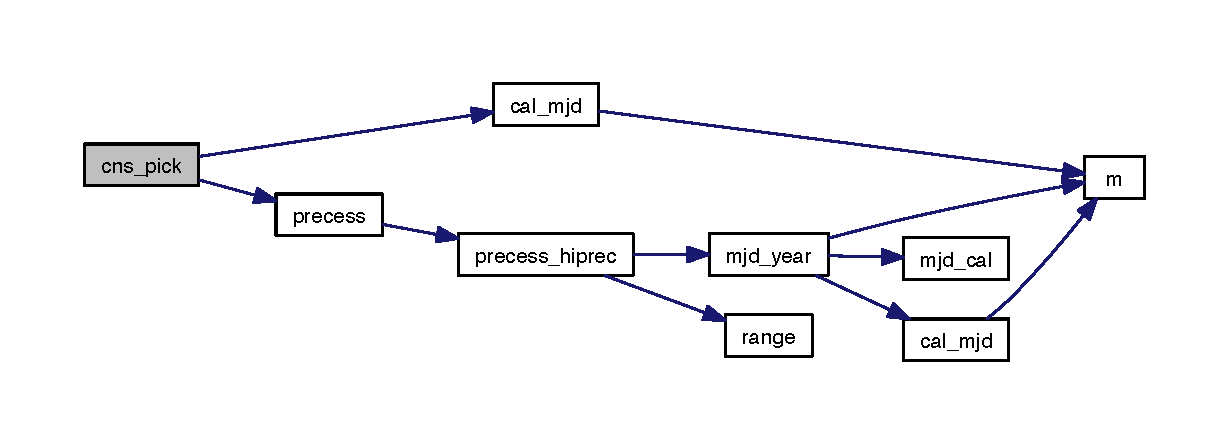
\includegraphics[width=350pt]{astro_8h_a76033e94f3dda39f889bf9f0999e1287_cgraph}
\end{center}
\end{figure}


\hypertarget{astro_8h_ae42663ccffbb2741a6b27abdfd032a72}{\index{astro.\-h@{astro.\-h}!comet@{comet}}
\index{comet@{comet}!astro.h@{astro.\-h}}
\subsubsection[{comet}]{\setlength{\rightskip}{0pt plus 5cm}void comet (
\begin{DoxyParamCaption}
\item[{double}]{m, }
\item[{double}]{ep, }
\item[{double}]{inc, }
\item[{double}]{ap, }
\item[{double}]{qp, }
\item[{double}]{om, }
\item[{double $\ast$}]{lpd, }
\item[{double $\ast$}]{psi, }
\item[{double $\ast$}]{rp, }
\item[{double $\ast$}]{rho, }
\item[{double $\ast$}]{lam, }
\item[{double $\ast$}]{bet}
\end{DoxyParamCaption}
)}}\label{astro_8h_ae42663ccffbb2741a6b27abdfd032a72}


Definition at line 31 of file comet.\-c.



Here is the call graph for this function\-:
\nopagebreak
\begin{figure}[H]
\begin{center}
\leavevmode
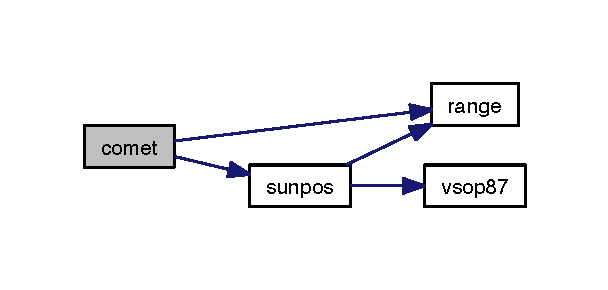
\includegraphics[width=292pt]{astro_8h_ae42663ccffbb2741a6b27abdfd032a72_cgraph}
\end{center}
\end{figure}




Here is the caller graph for this function\-:
\nopagebreak
\begin{figure}[H]
\begin{center}
\leavevmode
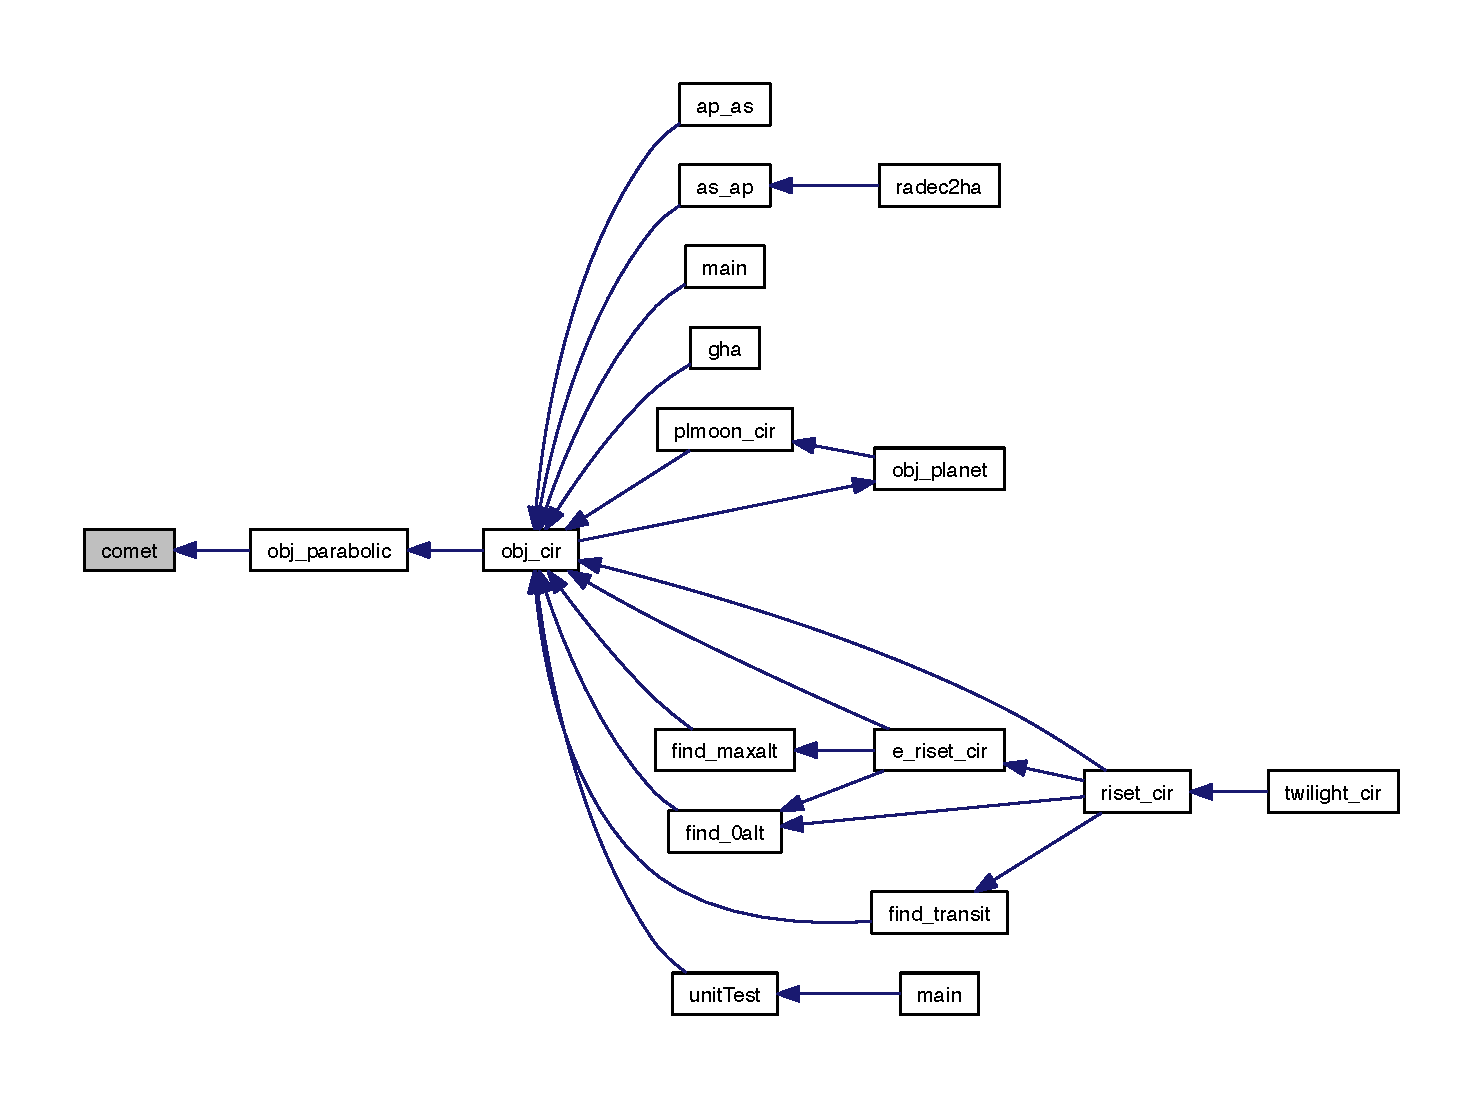
\includegraphics[width=350pt]{astro_8h_ae42663ccffbb2741a6b27abdfd032a72_icgraph}
\end{center}
\end{figure}


\hypertarget{astro_8h_a2cc4d4c161efb870b5b32ee2df721cc7}{\index{astro.\-h@{astro.\-h}!date\-Range\-O\-K@{date\-Range\-O\-K}}
\index{date\-Range\-O\-K@{date\-Range\-O\-K}!astro.h@{astro.\-h}}
\subsubsection[{date\-Range\-O\-K}]{\setlength{\rightskip}{0pt plus 5cm}int date\-Range\-O\-K (
\begin{DoxyParamCaption}
\item[{{\bf Now} $\ast$}]{np, }
\item[{{\bf Obj} $\ast$}]{op}
\end{DoxyParamCaption}
)}}\label{astro_8h_a2cc4d4c161efb870b5b32ee2df721cc7}


Definition at line 270 of file dbfmt.\-c.

\hypertarget{astro_8h_a3fcb82977d6cff1781d5977a04a041fc}{\index{astro.\-h@{astro.\-h}!db\-\_\-crack\-\_\-line@{db\-\_\-crack\-\_\-line}}
\index{db\-\_\-crack\-\_\-line@{db\-\_\-crack\-\_\-line}!astro.h@{astro.\-h}}
\subsubsection[{db\-\_\-crack\-\_\-line}]{\setlength{\rightskip}{0pt plus 5cm}int db\-\_\-crack\-\_\-line (
\begin{DoxyParamCaption}
\item[{char}]{s\mbox{[}$\,$\mbox{]}, }
\item[{{\bf Obj} $\ast$}]{op, }
\item[{char}]{nm\mbox{[}$\,$\mbox{]}\mbox{[}\-M\-A\-X\-N\-M\mbox{]}, }
\item[{int}]{nnm, }
\item[{char}]{whynot\mbox{[}$\,$\mbox{]}}
\end{DoxyParamCaption}
)}}\label{astro_8h_a3fcb82977d6cff1781d5977a04a041fc}


Definition at line 60 of file dbfmt.\-c.



Here is the call graph for this function\-:
\nopagebreak
\begin{figure}[H]
\begin{center}
\leavevmode
\includegraphics[width=350pt]{astro_8h_a3fcb82977d6cff1781d5977a04a041fc_cgraph}
\end{center}
\end{figure}




Here is the caller graph for this function\-:
\nopagebreak
\begin{figure}[H]
\begin{center}
\leavevmode
\includegraphics[width=350pt]{astro_8h_a3fcb82977d6cff1781d5977a04a041fc_icgraph}
\end{center}
\end{figure}


\hypertarget{astro_8h_a2eb175e79f59960b46a5a2acc1063283}{\index{astro.\-h@{astro.\-h}!db\-\_\-tle@{db\-\_\-tle}}
\index{db\-\_\-tle@{db\-\_\-tle}!astro.h@{astro.\-h}}
\subsubsection[{db\-\_\-tle}]{\setlength{\rightskip}{0pt plus 5cm}int db\-\_\-tle (
\begin{DoxyParamCaption}
\item[{char $\ast$}]{name, }
\item[{char $\ast$}]{l1, }
\item[{char $\ast$}]{l2, }
\item[{{\bf Obj} $\ast$}]{op}
\end{DoxyParamCaption}
)}}\label{astro_8h_a2eb175e79f59960b46a5a2acc1063283}


Definition at line 191 of file dbfmt.\-c.



Here is the call graph for this function\-:
\nopagebreak
\begin{figure}[H]
\begin{center}
\leavevmode
\includegraphics[width=350pt]{astro_8h_a2eb175e79f59960b46a5a2acc1063283_cgraph}
\end{center}
\end{figure}


\hypertarget{astro_8h_ab95713b7a3c2f31f438e5f5c70b72a7c}{\index{astro.\-h@{astro.\-h}!db\-\_\-write\-\_\-line@{db\-\_\-write\-\_\-line}}
\index{db\-\_\-write\-\_\-line@{db\-\_\-write\-\_\-line}!astro.h@{astro.\-h}}
\subsubsection[{db\-\_\-write\-\_\-line}]{\setlength{\rightskip}{0pt plus 5cm}void db\-\_\-write\-\_\-line (
\begin{DoxyParamCaption}
\item[{{\bf Obj} $\ast$}]{op, }
\item[{char $\ast$}]{lp}
\end{DoxyParamCaption}
)}}\label{astro_8h_ab95713b7a3c2f31f438e5f5c70b72a7c}
\hypertarget{astro_8h_ae88d15395987f2a4b5b389fa9e01b6a6}{\index{astro.\-h@{astro.\-h}!dbline\-\_\-candidate@{dbline\-\_\-candidate}}
\index{dbline\-\_\-candidate@{dbline\-\_\-candidate}!astro.h@{astro.\-h}}
\subsubsection[{dbline\-\_\-candidate}]{\setlength{\rightskip}{0pt plus 5cm}int dbline\-\_\-candidate (
\begin{DoxyParamCaption}
\item[{char}]{line\mbox{[}$\,$\mbox{]}}
\end{DoxyParamCaption}
)}}\label{astro_8h_ae88d15395987f2a4b5b389fa9e01b6a6}
\hypertarget{astro_8h_a8da023a45b428e345a893ef645591742}{\index{astro.\-h@{astro.\-h}!delra@{delra}}
\index{delra@{delra}!astro.h@{astro.\-h}}
\subsubsection[{delra}]{\setlength{\rightskip}{0pt plus 5cm}double delra (
\begin{DoxyParamCaption}
\item[{double}]{dra}
\end{DoxyParamCaption}
)}}\label{astro_8h_a8da023a45b428e345a893ef645591742}


Definition at line 467 of file misc.\-c.

\hypertarget{astro_8h_a890258e26664da3fc40d14e45396c5bc}{\index{astro.\-h@{astro.\-h}!deltat@{deltat}}
\index{deltat@{deltat}!astro.h@{astro.\-h}}
\subsubsection[{deltat}]{\setlength{\rightskip}{0pt plus 5cm}double deltat (
\begin{DoxyParamCaption}
\item[{double}]{m}
\end{DoxyParamCaption}
)}}\label{astro_8h_a890258e26664da3fc40d14e45396c5bc}


Definition at line 148 of file deltat.\-c.



Here is the call graph for this function\-:
\nopagebreak
\begin{figure}[H]
\begin{center}
\leavevmode
\includegraphics[width=350pt]{astro_8h_a890258e26664da3fc40d14e45396c5bc_cgraph}
\end{center}
\end{figure}




Here is the caller graph for this function\-:
\nopagebreak
\begin{figure}[H]
\begin{center}
\leavevmode
\includegraphics[width=216pt]{astro_8h_a890258e26664da3fc40d14e45396c5bc_icgraph}
\end{center}
\end{figure}


\hypertarget{astro_8h_a88b86fd88353155b80e3a0578eae61f1}{\index{astro.\-h@{astro.\-h}!ecl\-\_\-eq@{ecl\-\_\-eq}}
\index{ecl\-\_\-eq@{ecl\-\_\-eq}!astro.h@{astro.\-h}}
\subsubsection[{ecl\-\_\-eq}]{\setlength{\rightskip}{0pt plus 5cm}void ecl\-\_\-eq (
\begin{DoxyParamCaption}
\item[{double}]{m, }
\item[{double}]{lt, }
\item[{double}]{lg, }
\item[{double $\ast$}]{ra, }
\item[{double $\ast$}]{dec}
\end{DoxyParamCaption}
)}}\label{astro_8h_a88b86fd88353155b80e3a0578eae61f1}


Definition at line 32 of file eq\-\_\-ecl.\-c.



Here is the call graph for this function\-:
\nopagebreak
\begin{figure}[H]
\begin{center}
\leavevmode
\includegraphics[width=314pt]{astro_8h_a88b86fd88353155b80e3a0578eae61f1_cgraph}
\end{center}
\end{figure}




Here is the caller graph for this function\-:
\nopagebreak
\begin{figure}[H]
\begin{center}
\leavevmode
\includegraphics[width=350pt]{astro_8h_a88b86fd88353155b80e3a0578eae61f1_icgraph}
\end{center}
\end{figure}


\hypertarget{astro_8h_a92df2886db0f3b8b7f02e7ae3c074a58}{\index{astro.\-h@{astro.\-h}!eq\-\_\-ecl@{eq\-\_\-ecl}}
\index{eq\-\_\-ecl@{eq\-\_\-ecl}!astro.h@{astro.\-h}}
\subsubsection[{eq\-\_\-ecl}]{\setlength{\rightskip}{0pt plus 5cm}void eq\-\_\-ecl (
\begin{DoxyParamCaption}
\item[{double}]{m, }
\item[{double}]{ra, }
\item[{double}]{dec, }
\item[{double $\ast$}]{lt, }
\item[{double $\ast$}]{lg}
\end{DoxyParamCaption}
)}}\label{astro_8h_a92df2886db0f3b8b7f02e7ae3c074a58}


Definition at line 20 of file eq\-\_\-ecl.\-c.



Here is the call graph for this function\-:
\nopagebreak
\begin{figure}[H]
\begin{center}
\leavevmode
\includegraphics[width=314pt]{astro_8h_a92df2886db0f3b8b7f02e7ae3c074a58_cgraph}
\end{center}
\end{figure}




Here is the caller graph for this function\-:
\nopagebreak
\begin{figure}[H]
\begin{center}
\leavevmode
\includegraphics[width=350pt]{astro_8h_a92df2886db0f3b8b7f02e7ae3c074a58_icgraph}
\end{center}
\end{figure}


\hypertarget{astro_8h_a5a46db0cce1e03d715e082e0468b3762}{\index{astro.\-h@{astro.\-h}!eq\-\_\-gal@{eq\-\_\-gal}}
\index{eq\-\_\-gal@{eq\-\_\-gal}!astro.h@{astro.\-h}}
\subsubsection[{eq\-\_\-gal}]{\setlength{\rightskip}{0pt plus 5cm}void eq\-\_\-gal (
\begin{DoxyParamCaption}
\item[{double}]{m, }
\item[{double}]{ra, }
\item[{double}]{dec, }
\item[{double $\ast$}]{lt, }
\item[{double $\ast$}]{lg}
\end{DoxyParamCaption}
)}}\label{astro_8h_a5a46db0cce1e03d715e082e0468b3762}


Definition at line 27 of file eq\-\_\-gal.\-c.



Here is the call graph for this function\-:
\nopagebreak
\begin{figure}[H]
\begin{center}
\leavevmode
\includegraphics[width=350pt]{astro_8h_a5a46db0cce1e03d715e082e0468b3762_cgraph}
\end{center}
\end{figure}


\hypertarget{astro_8h_a3e9af80e9b2eb79ff71bd053e53d4f82}{\index{astro.\-h@{astro.\-h}!f\-\_\-scansexa@{f\-\_\-scansexa}}
\index{f\-\_\-scansexa@{f\-\_\-scansexa}!astro.h@{astro.\-h}}
\subsubsection[{f\-\_\-scansexa}]{\setlength{\rightskip}{0pt plus 5cm}int f\-\_\-scansexa (
\begin{DoxyParamCaption}
\item[{const char $\ast$}]{str, }
\item[{double $\ast$}]{dp}
\end{DoxyParamCaption}
)}}\label{astro_8h_a3e9af80e9b2eb79ff71bd053e53d4f82}


Definition at line 122 of file formats.\-c.



Here is the caller graph for this function\-:
\nopagebreak
\begin{figure}[H]
\begin{center}
\leavevmode
\includegraphics[width=350pt]{astro_8h_a3e9af80e9b2eb79ff71bd053e53d4f82_icgraph}
\end{center}
\end{figure}


\hypertarget{astro_8h_acb4c0000fa5b94721c8e2534b0d58396}{\index{astro.\-h@{astro.\-h}!f\-\_\-sscandate@{f\-\_\-sscandate}}
\index{f\-\_\-sscandate@{f\-\_\-sscandate}!astro.h@{astro.\-h}}
\subsubsection[{f\-\_\-sscandate}]{\setlength{\rightskip}{0pt plus 5cm}void f\-\_\-sscandate (
\begin{DoxyParamCaption}
\item[{char $\ast$}]{bp, }
\item[{int}]{pref, }
\item[{int $\ast$}]{m, }
\item[{double $\ast$}]{d, }
\item[{int $\ast$}]{y}
\end{DoxyParamCaption}
)}}\label{astro_8h_acb4c0000fa5b94721c8e2534b0d58396}


Definition at line 163 of file formats.\-c.



Here is the call graph for this function\-:
\nopagebreak
\begin{figure}[H]
\begin{center}
\leavevmode
\includegraphics[width=350pt]{astro_8h_acb4c0000fa5b94721c8e2534b0d58396_cgraph}
\end{center}
\end{figure}




Here is the caller graph for this function\-:
\nopagebreak
\begin{figure}[H]
\begin{center}
\leavevmode
\includegraphics[width=350pt]{astro_8h_acb4c0000fa5b94721c8e2534b0d58396_icgraph}
\end{center}
\end{figure}


\hypertarget{astro_8h_aad19fd4c699b772ab5155ff79df50d48}{\index{astro.\-h@{astro.\-h}!fs\-\_\-date@{fs\-\_\-date}}
\index{fs\-\_\-date@{fs\-\_\-date}!astro.h@{astro.\-h}}
\subsubsection[{fs\-\_\-date}]{\setlength{\rightskip}{0pt plus 5cm}int fs\-\_\-date (
\begin{DoxyParamCaption}
\item[{char}]{out\mbox{[}$\,$\mbox{]}, }
\item[{int}]{format, }
\item[{double}]{jd}
\end{DoxyParamCaption}
)}}\label{astro_8h_aad19fd4c699b772ab5155ff79df50d48}


Definition at line 84 of file formats.\-c.



Here is the call graph for this function\-:
\nopagebreak
\begin{figure}[H]
\begin{center}
\leavevmode
\includegraphics[width=220pt]{astro_8h_aad19fd4c699b772ab5155ff79df50d48_cgraph}
\end{center}
\end{figure}




Here is the caller graph for this function\-:
\nopagebreak
\begin{figure}[H]
\begin{center}
\leavevmode
\includegraphics[width=350pt]{astro_8h_aad19fd4c699b772ab5155ff79df50d48_icgraph}
\end{center}
\end{figure}


\hypertarget{astro_8h_ad1d4abef28e1ebc8198d6d667f947516}{\index{astro.\-h@{astro.\-h}!fs\-\_\-sexa@{fs\-\_\-sexa}}
\index{fs\-\_\-sexa@{fs\-\_\-sexa}!astro.h@{astro.\-h}}
\subsubsection[{fs\-\_\-sexa}]{\setlength{\rightskip}{0pt plus 5cm}int fs\-\_\-sexa (
\begin{DoxyParamCaption}
\item[{char $\ast$}]{out, }
\item[{double}]{a, }
\item[{int}]{w, }
\item[{int}]{fracbase}
\end{DoxyParamCaption}
)}}\label{astro_8h_ad1d4abef28e1ebc8198d6d667f947516}


Definition at line 21 of file formats.\-c.



Here is the call graph for this function\-:
\nopagebreak
\begin{figure}[H]
\begin{center}
\leavevmode
\includegraphics[width=196pt]{astro_8h_ad1d4abef28e1ebc8198d6d667f947516_cgraph}
\end{center}
\end{figure}




Here is the caller graph for this function\-:
\nopagebreak
\begin{figure}[H]
\begin{center}
\leavevmode
\includegraphics[width=350pt]{astro_8h_ad1d4abef28e1ebc8198d6d667f947516_icgraph}
\end{center}
\end{figure}


\hypertarget{astro_8h_a2c1a6a7369f932ae047ea0f6b54ef12a}{\index{astro.\-h@{astro.\-h}!gal\-\_\-eq@{gal\-\_\-eq}}
\index{gal\-\_\-eq@{gal\-\_\-eq}!astro.h@{astro.\-h}}
\subsubsection[{gal\-\_\-eq}]{\setlength{\rightskip}{0pt plus 5cm}void gal\-\_\-eq (
\begin{DoxyParamCaption}
\item[{double}]{m, }
\item[{double}]{lt, }
\item[{double}]{lg, }
\item[{double $\ast$}]{ra, }
\item[{double $\ast$}]{dec}
\end{DoxyParamCaption}
)}}\label{astro_8h_a2c1a6a7369f932ae047ea0f6b54ef12a}


Definition at line 39 of file eq\-\_\-gal.\-c.



Here is the call graph for this function\-:
\nopagebreak
\begin{figure}[H]
\begin{center}
\leavevmode
\includegraphics[width=350pt]{astro_8h_a2c1a6a7369f932ae047ea0f6b54ef12a_cgraph}
\end{center}
\end{figure}


\hypertarget{astro_8h_af9cb216dc50fbdba951f4dbe7f4c098e}{\index{astro.\-h@{astro.\-h}!get\-\_\-fields@{get\-\_\-fields}}
\index{get\-\_\-fields@{get\-\_\-fields}!astro.h@{astro.\-h}}
\subsubsection[{get\-\_\-fields}]{\setlength{\rightskip}{0pt plus 5cm}int get\-\_\-fields (
\begin{DoxyParamCaption}
\item[{char $\ast$}]{s, }
\item[{int}]{delim, }
\item[{char $\ast$}]{fields\mbox{[}$\,$\mbox{]}}
\end{DoxyParamCaption}
)}}\label{astro_8h_af9cb216dc50fbdba951f4dbe7f4c098e}


Definition at line 307 of file dbfmt.\-c.



Here is the caller graph for this function\-:
\nopagebreak
\begin{figure}[H]
\begin{center}
\leavevmode
\includegraphics[width=350pt]{astro_8h_af9cb216dc50fbdba951f4dbe7f4c098e_icgraph}
\end{center}
\end{figure}


\hypertarget{astro_8h_a402a3716f4b9767a1503543aa416bc10}{\index{astro.\-h@{astro.\-h}!get\-Built\-In\-Objs@{get\-Built\-In\-Objs}}
\index{get\-Built\-In\-Objs@{get\-Built\-In\-Objs}!astro.h@{astro.\-h}}
\subsubsection[{get\-Built\-In\-Objs}]{\setlength{\rightskip}{0pt plus 5cm}int get\-Built\-In\-Objs (
\begin{DoxyParamCaption}
\item[{{\bf Obj} $\ast$$\ast$}]{opp}
\end{DoxyParamCaption}
)}}\label{astro_8h_a402a3716f4b9767a1503543aa416bc10}


Definition at line 40 of file plmoon.\-c.



Here is the call graph for this function\-:
\nopagebreak
\begin{figure}[H]
\begin{center}
\leavevmode
\includegraphics[width=350pt]{astro_8h_a402a3716f4b9767a1503543aa416bc10_cgraph}
\end{center}
\end{figure}




Here is the caller graph for this function\-:
\nopagebreak
\begin{figure}[H]
\begin{center}
\leavevmode
\includegraphics[width=350pt]{astro_8h_a402a3716f4b9767a1503543aa416bc10_icgraph}
\end{center}
\end{figure}


\hypertarget{astro_8h_a6efd883b3f96c6bc244d5da7fe50e8f8}{\index{astro.\-h@{astro.\-h}!gha@{gha}}
\index{gha@{gha}!astro.h@{astro.\-h}}
\subsubsection[{gha}]{\setlength{\rightskip}{0pt plus 5cm}void gha (
\begin{DoxyParamCaption}
\item[{{\bf Now} $\ast$}]{np, }
\item[{{\bf Obj} $\ast$}]{op, }
\item[{double $\ast$}]{ghap}
\end{DoxyParamCaption}
)}}\label{astro_8h_a6efd883b3f96c6bc244d5da7fe50e8f8}


Definition at line 202 of file misc.\-c.



Here is the call graph for this function\-:
\nopagebreak
\begin{figure}[H]
\begin{center}
\leavevmode
\includegraphics[height=550pt]{astro_8h_a6efd883b3f96c6bc244d5da7fe50e8f8_cgraph}
\end{center}
\end{figure}


\hypertarget{astro_8h_a5e139c87095944a279aaded2b007dc0f}{\index{astro.\-h@{astro.\-h}!gk\-\_\-mag@{gk\-\_\-mag}}
\index{gk\-\_\-mag@{gk\-\_\-mag}!astro.h@{astro.\-h}}
\subsubsection[{gk\-\_\-mag}]{\setlength{\rightskip}{0pt plus 5cm}void gk\-\_\-mag (
\begin{DoxyParamCaption}
\item[{double}]{g, }
\item[{double}]{k, }
\item[{double}]{rp, }
\item[{double}]{rho, }
\item[{double $\ast$}]{mp}
\end{DoxyParamCaption}
)}}\label{astro_8h_a5e139c87095944a279aaded2b007dc0f}


Definition at line 343 of file misc.\-c.



Here is the caller graph for this function\-:
\nopagebreak
\begin{figure}[H]
\begin{center}
\leavevmode
\includegraphics[width=350pt]{astro_8h_a5e139c87095944a279aaded2b007dc0f_icgraph}
\end{center}
\end{figure}


\hypertarget{astro_8h_a948bae37b3103770aaeb0b98b919449c}{\index{astro.\-h@{astro.\-h}!gst\-\_\-utc@{gst\-\_\-utc}}
\index{gst\-\_\-utc@{gst\-\_\-utc}!astro.h@{astro.\-h}}
\subsubsection[{gst\-\_\-utc}]{\setlength{\rightskip}{0pt plus 5cm}void gst\-\_\-utc (
\begin{DoxyParamCaption}
\item[{double}]{m, }
\item[{double}]{gst, }
\item[{double $\ast$}]{utc}
\end{DoxyParamCaption}
)}}\label{astro_8h_a948bae37b3103770aaeb0b98b919449c}


Definition at line 28 of file utc\-\_\-gst.\-c.



Here is the call graph for this function\-:
\nopagebreak
\begin{figure}[H]
\begin{center}
\leavevmode
\includegraphics[width=286pt]{astro_8h_a948bae37b3103770aaeb0b98b919449c_cgraph}
\end{center}
\end{figure}


\hypertarget{astro_8h_a8ce2fb9152b3b6d728cda9ac4962378e}{\index{astro.\-h@{astro.\-h}!hadec\-\_\-aa@{hadec\-\_\-aa}}
\index{hadec\-\_\-aa@{hadec\-\_\-aa}!astro.h@{astro.\-h}}
\subsubsection[{hadec\-\_\-aa}]{\setlength{\rightskip}{0pt plus 5cm}void hadec\-\_\-aa (
\begin{DoxyParamCaption}
\item[{double}]{lt, }
\item[{double}]{ha, }
\item[{double}]{dec, }
\item[{double $\ast$}]{alt, }
\item[{double $\ast$}]{az}
\end{DoxyParamCaption}
)}}\label{astro_8h_a8ce2fb9152b3b6d728cda9ac4962378e}


Definition at line 31 of file aa\-\_\-hadec.\-c.



Here is the call graph for this function\-:
\nopagebreak
\begin{figure}[H]
\begin{center}
\leavevmode
\includegraphics[width=350pt]{astro_8h_a8ce2fb9152b3b6d728cda9ac4962378e_cgraph}
\end{center}
\end{figure}




Here is the caller graph for this function\-:
\nopagebreak
\begin{figure}[H]
\begin{center}
\leavevmode
\includegraphics[width=350pt]{astro_8h_a8ce2fb9152b3b6d728cda9ac4962378e_icgraph}
\end{center}
\end{figure}


\hypertarget{astro_8h_a2362d7460a3a9f46007e0faf2e913bd1}{\index{astro.\-h@{astro.\-h}!heliocorr@{heliocorr}}
\index{heliocorr@{heliocorr}!astro.h@{astro.\-h}}
\subsubsection[{heliocorr}]{\setlength{\rightskip}{0pt plus 5cm}void heliocorr (
\begin{DoxyParamCaption}
\item[{double}]{jd, }
\item[{double}]{ra, }
\item[{double}]{dec, }
\item[{double $\ast$}]{hcp}
\end{DoxyParamCaption}
)}}\label{astro_8h_a2362d7460a3a9f46007e0faf2e913bd1}


Definition at line 13 of file helio.\-c.



Here is the call graph for this function\-:
\nopagebreak
\begin{figure}[H]
\begin{center}
\leavevmode
\includegraphics[width=350pt]{astro_8h_a2362d7460a3a9f46007e0faf2e913bd1_cgraph}
\end{center}
\end{figure}


\hypertarget{astro_8h_a2138a902426608f08fbba29150ad7541}{\index{astro.\-h@{astro.\-h}!hg\-\_\-mag@{hg\-\_\-mag}}
\index{hg\-\_\-mag@{hg\-\_\-mag}!astro.h@{astro.\-h}}
\subsubsection[{hg\-\_\-mag}]{\setlength{\rightskip}{0pt plus 5cm}void hg\-\_\-mag (
\begin{DoxyParamCaption}
\item[{double}]{h, }
\item[{double}]{g, }
\item[{double}]{rp, }
\item[{double}]{rho, }
\item[{double}]{rsn, }
\item[{double $\ast$}]{mp}
\end{DoxyParamCaption}
)}}\label{astro_8h_a2138a902426608f08fbba29150ad7541}


Definition at line 287 of file misc.\-c.



Here is the caller graph for this function\-:
\nopagebreak
\begin{figure}[H]
\begin{center}
\leavevmode
\includegraphics[width=350pt]{astro_8h_a2138a902426608f08fbba29150ad7541_icgraph}
\end{center}
\end{figure}


\hypertarget{astro_8h_ab3dce3d5ba37b8fdcea3d9396f2632e3}{\index{astro.\-h@{astro.\-h}!is\-\_\-deepsky@{is\-\_\-deepsky}}
\index{is\-\_\-deepsky@{is\-\_\-deepsky}!astro.h@{astro.\-h}}
\subsubsection[{is\-\_\-deepsky}]{\setlength{\rightskip}{0pt plus 5cm}int is\-\_\-deepsky (
\begin{DoxyParamCaption}
\item[{{\bf Obj} $\ast$}]{op}
\end{DoxyParamCaption}
)}}\label{astro_8h_ab3dce3d5ba37b8fdcea3d9396f2632e3}


Definition at line 480 of file misc.\-c.

\hypertarget{astro_8h_a42b0c880525bbb93e777c9b9b41df324}{\index{astro.\-h@{astro.\-h}!isleapyear@{isleapyear}}
\index{isleapyear@{isleapyear}!astro.h@{astro.\-h}}
\subsubsection[{isleapyear}]{\setlength{\rightskip}{0pt plus 5cm}int isleapyear (
\begin{DoxyParamCaption}
\item[{int}]{year}
\end{DoxyParamCaption}
)}}\label{astro_8h_a42b0c880525bbb93e777c9b9b41df324}


Definition at line 142 of file mjd.\-c.



Here is the caller graph for this function\-:
\nopagebreak
\begin{figure}[H]
\begin{center}
\leavevmode
\includegraphics[width=350pt]{astro_8h_a42b0c880525bbb93e777c9b9b41df324_icgraph}
\end{center}
\end{figure}


\hypertarget{astro_8h_a28756dff51966b2e9c4c54abca24df6b}{\index{astro.\-h@{astro.\-h}!jupiter\-\_\-data@{jupiter\-\_\-data}}
\index{jupiter\-\_\-data@{jupiter\-\_\-data}!astro.h@{astro.\-h}}
\subsubsection[{jupiter\-\_\-data}]{\setlength{\rightskip}{0pt plus 5cm}void jupiter\-\_\-data (
\begin{DoxyParamCaption}
\item[{double}]{Mjd, }
\item[{char}]{dir\mbox{[}$\,$\mbox{]}, }
\item[{{\bf Obj} $\ast$}]{sop, }
\item[{{\bf Obj} $\ast$}]{jop, }
\item[{double $\ast$}]{jupsize, }
\item[{double $\ast$}]{cml\-I, }
\item[{double $\ast$}]{cml\-I\-I, }
\item[{double $\ast$}]{polera, }
\item[{double $\ast$}]{poledec, }
\item[{{\bf Moon\-Data}}]{md\mbox{[}\-J\-\_\-\-N\-M\-O\-O\-N\-S\mbox{]}}
\end{DoxyParamCaption}
)}}\label{astro_8h_a28756dff51966b2e9c4c54abca24df6b}


Definition at line 47 of file jupmoon.\-c.



Here is the call graph for this function\-:
\nopagebreak
\begin{figure}[H]
\begin{center}
\leavevmode
\includegraphics[width=350pt]{astro_8h_a28756dff51966b2e9c4c54abca24df6b_cgraph}
\end{center}
\end{figure}




Here is the caller graph for this function\-:
\nopagebreak
\begin{figure}[H]
\begin{center}
\leavevmode
\includegraphics[width=350pt]{astro_8h_a28756dff51966b2e9c4c54abca24df6b_icgraph}
\end{center}
\end{figure}


\hypertarget{astro_8h_a444e1490c6862e31db0cd54fb2fd9534}{\index{astro.\-h@{astro.\-h}!lc@{lc}}
\index{lc@{lc}!astro.h@{astro.\-h}}
\subsubsection[{lc}]{\setlength{\rightskip}{0pt plus 5cm}int lc (
\begin{DoxyParamCaption}
\item[{int}]{cx, }
\item[{int}]{cy, }
\item[{int}]{cw, }
\item[{int}]{x1, }
\item[{int}]{y1, }
\item[{int}]{x2, }
\item[{int}]{y2, }
\item[{int $\ast$}]{sx1, }
\item[{int $\ast$}]{sy1, }
\item[{int $\ast$}]{sx2, }
\item[{int $\ast$}]{sy2}
\end{DoxyParamCaption}
)}}\label{astro_8h_a444e1490c6862e31db0cd54fb2fd9534}


Definition at line 229 of file misc.\-c.

\hypertarget{astro_8h_a42d82e732568f68846d2a138e7bce05f}{\index{astro.\-h@{astro.\-h}!llibration@{llibration}}
\index{llibration@{llibration}!astro.h@{astro.\-h}}
\subsubsection[{llibration}]{\setlength{\rightskip}{0pt plus 5cm}void llibration (
\begin{DoxyParamCaption}
\item[{double}]{J\-D, }
\item[{double $\ast$}]{llatp, }
\item[{double $\ast$}]{llonp}
\end{DoxyParamCaption}
)}}\label{astro_8h_a42d82e732568f68846d2a138e7bce05f}


Definition at line 2201 of file libration.\-c.



Here is the call graph for this function\-:
\nopagebreak
\begin{figure}[H]
\begin{center}
\leavevmode
\includegraphics[width=350pt]{astro_8h_a42d82e732568f68846d2a138e7bce05f_cgraph}
\end{center}
\end{figure}


\hypertarget{astro_8h_a35dd39f63546ec1e293505bf953ac983}{\index{astro.\-h@{astro.\-h}!magdecl@{magdecl}}
\index{magdecl@{magdecl}!astro.h@{astro.\-h}}
\subsubsection[{magdecl}]{\setlength{\rightskip}{0pt plus 5cm}int magdecl (
\begin{DoxyParamCaption}
\item[{double}]{l, }
\item[{double}]{L, }
\item[{double}]{e, }
\item[{double}]{y, }
\item[{char $\ast$}]{dir, }
\item[{double $\ast$}]{dp, }
\item[{char $\ast$}]{err}
\end{DoxyParamCaption}
)}}\label{astro_8h_a35dd39f63546ec1e293505bf953ac983}


Definition at line 27 of file magdecl.\-c.



Here is the call graph for this function\-:
\nopagebreak
\begin{figure}[H]
\begin{center}
\leavevmode
\includegraphics[width=350pt]{astro_8h_a35dd39f63546ec1e293505bf953ac983_cgraph}
\end{center}
\end{figure}


\hypertarget{astro_8h_a21e061ae8563510de4bf8344d28ca66b}{\index{astro.\-h@{astro.\-h}!magdiam@{magdiam}}
\index{magdiam@{magdiam}!astro.h@{astro.\-h}}
\subsubsection[{magdiam}]{\setlength{\rightskip}{0pt plus 5cm}int magdiam (
\begin{DoxyParamCaption}
\item[{int}]{fmag, }
\item[{int}]{magstp, }
\item[{double}]{scale, }
\item[{double}]{mag, }
\item[{double}]{size}
\end{DoxyParamCaption}
)}}\label{astro_8h_a21e061ae8563510de4bf8344d28ca66b}


Definition at line 321 of file misc.\-c.

\hypertarget{astro_8h_af45e2db2d4f8e60cbc95eed7d14e1619}{\index{astro.\-h@{astro.\-h}!marsm\-\_\-data@{marsm\-\_\-data}}
\index{marsm\-\_\-data@{marsm\-\_\-data}!astro.h@{astro.\-h}}
\subsubsection[{marsm\-\_\-data}]{\setlength{\rightskip}{0pt plus 5cm}void marsm\-\_\-data (
\begin{DoxyParamCaption}
\item[{double}]{Mjd, }
\item[{char}]{dir\mbox{[}$\,$\mbox{]}, }
\item[{{\bf Obj} $\ast$}]{sop, }
\item[{{\bf Obj} $\ast$}]{mop, }
\item[{double $\ast$}]{marssize, }
\item[{double $\ast$}]{polera, }
\item[{double $\ast$}]{poledec, }
\item[{{\bf Moon\-Data}}]{md\mbox{[}\-M\-\_\-\-N\-M\-O\-O\-N\-S\mbox{]}}
\end{DoxyParamCaption}
)}}\label{astro_8h_af45e2db2d4f8e60cbc95eed7d14e1619}


Definition at line 41 of file marsmoon.\-c.



Here is the call graph for this function\-:
\nopagebreak
\begin{figure}[H]
\begin{center}
\leavevmode
\includegraphics[width=350pt]{astro_8h_af45e2db2d4f8e60cbc95eed7d14e1619_cgraph}
\end{center}
\end{figure}




Here is the caller graph for this function\-:
\nopagebreak
\begin{figure}[H]
\begin{center}
\leavevmode
\includegraphics[width=350pt]{astro_8h_af45e2db2d4f8e60cbc95eed7d14e1619_icgraph}
\end{center}
\end{figure}


\hypertarget{astro_8h_ad60136599f12f591b12426c97833b446}{\index{astro.\-h@{astro.\-h}!mjd\-\_\-cal@{mjd\-\_\-cal}}
\index{mjd\-\_\-cal@{mjd\-\_\-cal}!astro.h@{astro.\-h}}
\subsubsection[{mjd\-\_\-cal}]{\setlength{\rightskip}{0pt plus 5cm}void mjd\-\_\-cal (
\begin{DoxyParamCaption}
\item[{double}]{m, }
\item[{int $\ast$}]{mn, }
\item[{double $\ast$}]{dy, }
\item[{int $\ast$}]{yr}
\end{DoxyParamCaption}
)}}\label{astro_8h_ad60136599f12f591b12426c97833b446}


Definition at line 59 of file mjd.\-c.



Here is the caller graph for this function\-:
\nopagebreak
\begin{figure}[H]
\begin{center}
\leavevmode
\includegraphics[width=350pt]{astro_8h_ad60136599f12f591b12426c97833b446_icgraph}
\end{center}
\end{figure}


\hypertarget{astro_8h_a3cf3e9c878a1800e4b4bfe551d1ec392}{\index{astro.\-h@{astro.\-h}!mjd\-\_\-day@{mjd\-\_\-day}}
\index{mjd\-\_\-day@{mjd\-\_\-day}!astro.h@{astro.\-h}}
\subsubsection[{mjd\-\_\-day}]{\setlength{\rightskip}{0pt plus 5cm}double mjd\-\_\-day (
\begin{DoxyParamCaption}
\item[{double}]{jd}
\end{DoxyParamCaption}
)}}\label{astro_8h_a3cf3e9c878a1800e4b4bfe551d1ec392}


Definition at line 219 of file mjd.\-c.



Here is the caller graph for this function\-:
\nopagebreak
\begin{figure}[H]
\begin{center}
\leavevmode
\includegraphics[width=350pt]{astro_8h_a3cf3e9c878a1800e4b4bfe551d1ec392_icgraph}
\end{center}
\end{figure}


\hypertarget{astro_8h_a9c71d7ce9aff1e4d84228c0e14eb2658}{\index{astro.\-h@{astro.\-h}!mjd\-\_\-dayno@{mjd\-\_\-dayno}}
\index{mjd\-\_\-dayno@{mjd\-\_\-dayno}!astro.h@{astro.\-h}}
\subsubsection[{mjd\-\_\-dayno}]{\setlength{\rightskip}{0pt plus 5cm}void mjd\-\_\-dayno (
\begin{DoxyParamCaption}
\item[{double}]{jd, }
\item[{int $\ast$}]{yr, }
\item[{double $\ast$}]{dy}
\end{DoxyParamCaption}
)}}\label{astro_8h_a9c71d7ce9aff1e4d84228c0e14eb2658}


Definition at line 161 of file mjd.\-c.



Here is the call graph for this function\-:
\nopagebreak
\begin{figure}[H]
\begin{center}
\leavevmode
\includegraphics[width=350pt]{astro_8h_a9c71d7ce9aff1e4d84228c0e14eb2658_cgraph}
\end{center}
\end{figure}




Here is the caller graph for this function\-:
\nopagebreak
\begin{figure}[H]
\begin{center}
\leavevmode
\includegraphics[width=350pt]{astro_8h_a9c71d7ce9aff1e4d84228c0e14eb2658_icgraph}
\end{center}
\end{figure}


\hypertarget{astro_8h_a2c0aa6510622ae4d96d8170cf87161c6}{\index{astro.\-h@{astro.\-h}!mjd\-\_\-dow@{mjd\-\_\-dow}}
\index{mjd\-\_\-dow@{mjd\-\_\-dow}!astro.h@{astro.\-h}}
\subsubsection[{mjd\-\_\-dow}]{\setlength{\rightskip}{0pt plus 5cm}int mjd\-\_\-dow (
\begin{DoxyParamCaption}
\item[{double}]{m, }
\item[{int $\ast$}]{dow}
\end{DoxyParamCaption}
)}}\label{astro_8h_a2c0aa6510622ae4d96d8170cf87161c6}


Definition at line 121 of file mjd.\-c.

\hypertarget{astro_8h_a440f08f6a390485f18aab9eb99e14617}{\index{astro.\-h@{astro.\-h}!mjd\-\_\-dpm@{mjd\-\_\-dpm}}
\index{mjd\-\_\-dpm@{mjd\-\_\-dpm}!astro.h@{astro.\-h}}
\subsubsection[{mjd\-\_\-dpm}]{\setlength{\rightskip}{0pt plus 5cm}void mjd\-\_\-dpm (
\begin{DoxyParamCaption}
\item[{double}]{m, }
\item[{int $\ast$}]{ndays}
\end{DoxyParamCaption}
)}}\label{astro_8h_a440f08f6a390485f18aab9eb99e14617}


Definition at line 149 of file mjd.\-c.



Here is the call graph for this function\-:
\nopagebreak
\begin{figure}[H]
\begin{center}
\leavevmode
\includegraphics[width=236pt]{astro_8h_a440f08f6a390485f18aab9eb99e14617_cgraph}
\end{center}
\end{figure}


\hypertarget{astro_8h_aa287e7d7be3e88eed3610d15deaaea5b}{\index{astro.\-h@{astro.\-h}!mjd\-\_\-hr@{mjd\-\_\-hr}}
\index{mjd\-\_\-hr@{mjd\-\_\-hr}!astro.h@{astro.\-h}}
\subsubsection[{mjd\-\_\-hr}]{\setlength{\rightskip}{0pt plus 5cm}double mjd\-\_\-hr (
\begin{DoxyParamCaption}
\item[{double}]{jd}
\end{DoxyParamCaption}
)}}\label{astro_8h_aa287e7d7be3e88eed3610d15deaaea5b}


Definition at line 226 of file mjd.\-c.



Here is the call graph for this function\-:
\nopagebreak
\begin{figure}[H]
\begin{center}
\leavevmode
\includegraphics[width=218pt]{astro_8h_aa287e7d7be3e88eed3610d15deaaea5b_cgraph}
\end{center}
\end{figure}




Here is the caller graph for this function\-:
\nopagebreak
\begin{figure}[H]
\begin{center}
\leavevmode
\includegraphics[width=350pt]{astro_8h_aa287e7d7be3e88eed3610d15deaaea5b_icgraph}
\end{center}
\end{figure}


\hypertarget{astro_8h_afe66e4f206d9a07bb390e71fc3522986}{\index{astro.\-h@{astro.\-h}!mjd\-\_\-year@{mjd\-\_\-year}}
\index{mjd\-\_\-year@{mjd\-\_\-year}!astro.h@{astro.\-h}}
\subsubsection[{mjd\-\_\-year}]{\setlength{\rightskip}{0pt plus 5cm}void mjd\-\_\-year (
\begin{DoxyParamCaption}
\item[{double}]{m, }
\item[{double $\ast$}]{yr}
\end{DoxyParamCaption}
)}}\label{astro_8h_afe66e4f206d9a07bb390e71fc3522986}


Definition at line 175 of file mjd.\-c.



Here is the call graph for this function\-:
\nopagebreak
\begin{figure}[H]
\begin{center}
\leavevmode
\includegraphics[width=290pt]{astro_8h_afe66e4f206d9a07bb390e71fc3522986_cgraph}
\end{center}
\end{figure}




Here is the caller graph for this function\-:
\nopagebreak
\begin{figure}[H]
\begin{center}
\leavevmode
\includegraphics[width=350pt]{astro_8h_afe66e4f206d9a07bb390e71fc3522986_icgraph}
\end{center}
\end{figure}


\hypertarget{astro_8h_a56ed70df83f91389b30f9f219fc20a2c}{\index{astro.\-h@{astro.\-h}!mm\-\_\-mjed@{mm\-\_\-mjed}}
\index{mm\-\_\-mjed@{mm\-\_\-mjed}!astro.h@{astro.\-h}}
\subsubsection[{mm\-\_\-mjed}]{\setlength{\rightskip}{0pt plus 5cm}double mm\-\_\-mjed (
\begin{DoxyParamCaption}
\item[{{\bf Now} $\ast$}]{np}
\end{DoxyParamCaption}
)}}\label{astro_8h_a56ed70df83f91389b30f9f219fc20a2c}


Definition at line 36 of file auxil.\-c.



Here is the call graph for this function\-:
\nopagebreak
\begin{figure}[H]
\begin{center}
\leavevmode
\includegraphics[width=350pt]{astro_8h_a56ed70df83f91389b30f9f219fc20a2c_cgraph}
\end{center}
\end{figure}


\hypertarget{astro_8h_a2ea945b83e3df3636a5562d0ba819194}{\index{astro.\-h@{astro.\-h}!moon@{moon}}
\index{moon@{moon}!astro.h@{astro.\-h}}
\subsubsection[{moon}]{\setlength{\rightskip}{0pt plus 5cm}void moon (
\begin{DoxyParamCaption}
\item[{double}]{m, }
\item[{double $\ast$}]{lam, }
\item[{double $\ast$}]{bet, }
\item[{double $\ast$}]{rho, }
\item[{double $\ast$}]{msp, }
\item[{double $\ast$}]{mdp}
\end{DoxyParamCaption}
)}}\label{astro_8h_a2ea945b83e3df3636a5562d0ba819194}


Definition at line 3440 of file moon.\-c.



Here is the call graph for this function\-:
\nopagebreak
\begin{figure}[H]
\begin{center}
\leavevmode
\includegraphics[width=300pt]{astro_8h_a2ea945b83e3df3636a5562d0ba819194_cgraph}
\end{center}
\end{figure}




Here is the caller graph for this function\-:
\nopagebreak
\begin{figure}[H]
\begin{center}
\leavevmode
\includegraphics[width=350pt]{astro_8h_a2ea945b83e3df3636a5562d0ba819194_icgraph}
\end{center}
\end{figure}


\hypertarget{astro_8h_a2b580af984adcdec784ee9fd6e556cde}{\index{astro.\-h@{astro.\-h}!moon\-\_\-colong@{moon\-\_\-colong}}
\index{moon\-\_\-colong@{moon\-\_\-colong}!astro.h@{astro.\-h}}
\subsubsection[{moon\-\_\-colong}]{\setlength{\rightskip}{0pt plus 5cm}void moon\-\_\-colong (
\begin{DoxyParamCaption}
\item[{double}]{jd, }
\item[{double}]{lt, }
\item[{double}]{lg, }
\item[{double $\ast$}]{cp, }
\item[{double $\ast$}]{kp, }
\item[{double $\ast$}]{ap, }
\item[{double $\ast$}]{sp}
\end{DoxyParamCaption}
)}}\label{astro_8h_a2b580af984adcdec784ee9fd6e556cde}


Definition at line 25 of file mooncolong.\-c.



Here is the call graph for this function\-:
\nopagebreak
\begin{figure}[H]
\begin{center}
\leavevmode
\includegraphics[width=252pt]{astro_8h_a2b580af984adcdec784ee9fd6e556cde_cgraph}
\end{center}
\end{figure}


\hypertarget{astro_8h_a8aea5265249503f0a0687b4b7350e8ea}{\index{astro.\-h@{astro.\-h}!moonnf@{moonnf}}
\index{moonnf@{moonnf}!astro.h@{astro.\-h}}
\subsubsection[{moonnf}]{\setlength{\rightskip}{0pt plus 5cm}void moonnf (
\begin{DoxyParamCaption}
\item[{double}]{mj, }
\item[{double $\ast$}]{mjn, }
\item[{double $\ast$}]{mjf}
\end{DoxyParamCaption}
)}}\label{astro_8h_a8aea5265249503f0a0687b4b7350e8ea}


Definition at line 17 of file moonnf.\-c.



Here is the call graph for this function\-:
\nopagebreak
\begin{figure}[H]
\begin{center}
\leavevmode
\includegraphics[width=282pt]{astro_8h_a8aea5265249503f0a0687b4b7350e8ea_cgraph}
\end{center}
\end{figure}


\hypertarget{astro_8h_ad9b069df7c280a1584d54cd0be01c585}{\index{astro.\-h@{astro.\-h}!msa\-\_\-atlas@{msa\-\_\-atlas}}
\index{msa\-\_\-atlas@{msa\-\_\-atlas}!astro.h@{astro.\-h}}
\subsubsection[{msa\-\_\-atlas}]{\setlength{\rightskip}{0pt plus 5cm}char$\ast$ msa\-\_\-atlas (
\begin{DoxyParamCaption}
\item[{double}]{ra, }
\item[{double}]{dec}
\end{DoxyParamCaption}
)}}\label{astro_8h_ad9b069df7c280a1584d54cd0be01c585}


Definition at line 30 of file atlas.\-c.

\hypertarget{astro_8h_a523b0a2df5b35cd9da39a4d5bd1ff1d6}{\index{astro.\-h@{astro.\-h}!now\-\_\-lst@{now\-\_\-lst}}
\index{now\-\_\-lst@{now\-\_\-lst}!astro.h@{astro.\-h}}
\subsubsection[{now\-\_\-lst}]{\setlength{\rightskip}{0pt plus 5cm}void now\-\_\-lst (
\begin{DoxyParamCaption}
\item[{{\bf Now} $\ast$}]{np, }
\item[{double $\ast$}]{lstp}
\end{DoxyParamCaption}
)}}\label{astro_8h_a523b0a2df5b35cd9da39a4d5bd1ff1d6}


Definition at line 158 of file misc.\-c.



Here is the call graph for this function\-:
\nopagebreak
\begin{figure}[H]
\begin{center}
\leavevmode
\includegraphics[width=350pt]{astro_8h_a523b0a2df5b35cd9da39a4d5bd1ff1d6_cgraph}
\end{center}
\end{figure}




Here is the caller graph for this function\-:
\nopagebreak
\begin{figure}[H]
\begin{center}
\leavevmode
\includegraphics[width=350pt]{astro_8h_a523b0a2df5b35cd9da39a4d5bd1ff1d6_icgraph}
\end{center}
\end{figure}


\hypertarget{astro_8h_a49fad3f928496f345c65181417d89f2c}{\index{astro.\-h@{astro.\-h}!nut\-\_\-eq@{nut\-\_\-eq}}
\index{nut\-\_\-eq@{nut\-\_\-eq}!astro.h@{astro.\-h}}
\subsubsection[{nut\-\_\-eq}]{\setlength{\rightskip}{0pt plus 5cm}void nut\-\_\-eq (
\begin{DoxyParamCaption}
\item[{double}]{m, }
\item[{double $\ast$}]{ra, }
\item[{double $\ast$}]{dec}
\end{DoxyParamCaption}
)}}\label{astro_8h_a49fad3f928496f345c65181417d89f2c}


Definition at line 373 of file nutation.\-c.



Here is the call graph for this function\-:
\nopagebreak
\begin{figure}[H]
\begin{center}
\leavevmode
\includegraphics[width=296pt]{astro_8h_a49fad3f928496f345c65181417d89f2c_cgraph}
\end{center}
\end{figure}




Here is the caller graph for this function\-:
\nopagebreak
\begin{figure}[H]
\begin{center}
\leavevmode
\includegraphics[width=350pt]{astro_8h_a49fad3f928496f345c65181417d89f2c_icgraph}
\end{center}
\end{figure}


\hypertarget{astro_8h_a96bb2600a9686001e9137555bd49ae16}{\index{astro.\-h@{astro.\-h}!nutation@{nutation}}
\index{nutation@{nutation}!astro.h@{astro.\-h}}
\subsubsection[{nutation}]{\setlength{\rightskip}{0pt plus 5cm}void nutation (
\begin{DoxyParamCaption}
\item[{double}]{m, }
\item[{double $\ast$}]{deps, }
\item[{double $\ast$}]{dpsi}
\end{DoxyParamCaption}
)}}\label{astro_8h_a96bb2600a9686001e9137555bd49ae16}


Definition at line 274 of file nutation.\-c.



Here is the caller graph for this function\-:
\nopagebreak
\begin{figure}[H]
\begin{center}
\leavevmode
\includegraphics[width=350pt]{astro_8h_a96bb2600a9686001e9137555bd49ae16_icgraph}
\end{center}
\end{figure}


\hypertarget{astro_8h_a88029bd0976d52e82ec40e1b9230d54a}{\index{astro.\-h@{astro.\-h}!obj\-\_\-cir@{obj\-\_\-cir}}
\index{obj\-\_\-cir@{obj\-\_\-cir}!astro.h@{astro.\-h}}
\subsubsection[{obj\-\_\-cir}]{\setlength{\rightskip}{0pt plus 5cm}int obj\-\_\-cir (
\begin{DoxyParamCaption}
\item[{{\bf Now} $\ast$}]{np, }
\item[{{\bf Obj} $\ast$}]{op}
\end{DoxyParamCaption}
)}}\label{astro_8h_a88029bd0976d52e82ec40e1b9230d54a}


Definition at line 41 of file circum.\-c.



Here is the call graph for this function\-:
\nopagebreak
\begin{figure}[H]
\begin{center}
\leavevmode
\includegraphics[height=550pt]{astro_8h_a88029bd0976d52e82ec40e1b9230d54a_cgraph}
\end{center}
\end{figure}




Here is the caller graph for this function\-:
\nopagebreak
\begin{figure}[H]
\begin{center}
\leavevmode
\includegraphics[width=350pt]{astro_8h_a88029bd0976d52e82ec40e1b9230d54a_icgraph}
\end{center}
\end{figure}


\hypertarget{astro_8h_ac4299d6955dec032146edcdb03d20f82}{\index{astro.\-h@{astro.\-h}!obj\-\_\-description@{obj\-\_\-description}}
\index{obj\-\_\-description@{obj\-\_\-description}!astro.h@{astro.\-h}}
\subsubsection[{obj\-\_\-description}]{\setlength{\rightskip}{0pt plus 5cm}char$\ast$ obj\-\_\-description (
\begin{DoxyParamCaption}
\item[{{\bf Obj} $\ast$}]{op}
\end{DoxyParamCaption}
)}}\label{astro_8h_ac4299d6955dec032146edcdb03d20f82}


Definition at line 57 of file misc.\-c.



Here is the call graph for this function\-:
\nopagebreak
\begin{figure}[H]
\begin{center}
\leavevmode
\includegraphics[width=350pt]{astro_8h_ac4299d6955dec032146edcdb03d20f82_cgraph}
\end{center}
\end{figure}


\hypertarget{astro_8h_a33e16bf55d33a63934a19835b20784f0}{\index{astro.\-h@{astro.\-h}!obj\-\_\-earthsat@{obj\-\_\-earthsat}}
\index{obj\-\_\-earthsat@{obj\-\_\-earthsat}!astro.h@{astro.\-h}}
\subsubsection[{obj\-\_\-earthsat}]{\setlength{\rightskip}{0pt plus 5cm}int obj\-\_\-earthsat (
\begin{DoxyParamCaption}
\item[{{\bf Now} $\ast$}]{np, }
\item[{{\bf Obj} $\ast$}]{op}
\end{DoxyParamCaption}
)}}\label{astro_8h_a33e16bf55d33a63934a19835b20784f0}


Definition at line 133 of file earthsat.\-c.



Here is the call graph for this function\-:
\nopagebreak
\begin{figure}[H]
\begin{center}
\leavevmode
\includegraphics[width=350pt]{astro_8h_a33e16bf55d33a63934a19835b20784f0_cgraph}
\end{center}
\end{figure}




Here is the caller graph for this function\-:
\nopagebreak
\begin{figure}[H]
\begin{center}
\leavevmode
\includegraphics[width=350pt]{astro_8h_a33e16bf55d33a63934a19835b20784f0_icgraph}
\end{center}
\end{figure}


\hypertarget{astro_8h_a3ac3532b3e3aa09dc34aaf1936cf4696}{\index{astro.\-h@{astro.\-h}!obliquity@{obliquity}}
\index{obliquity@{obliquity}!astro.h@{astro.\-h}}
\subsubsection[{obliquity}]{\setlength{\rightskip}{0pt plus 5cm}void obliquity (
\begin{DoxyParamCaption}
\item[{double}]{m, }
\item[{double $\ast$}]{eps}
\end{DoxyParamCaption}
)}}\label{astro_8h_a3ac3532b3e3aa09dc34aaf1936cf4696}


Definition at line 11 of file obliq.\-c.



Here is the caller graph for this function\-:
\nopagebreak
\begin{figure}[H]
\begin{center}
\leavevmode
\includegraphics[width=350pt]{astro_8h_a3ac3532b3e3aa09dc34aaf1936cf4696_icgraph}
\end{center}
\end{figure}


\hypertarget{astro_8h_a2dcca251440294005ba00eb2b9ab1212}{\index{astro.\-h@{astro.\-h}!parallactic\-L\-D\-A@{parallactic\-L\-D\-A}}
\index{parallactic\-L\-D\-A@{parallactic\-L\-D\-A}!astro.h@{astro.\-h}}
\subsubsection[{parallactic\-L\-D\-A}]{\setlength{\rightskip}{0pt plus 5cm}double parallactic\-L\-D\-A (
\begin{DoxyParamCaption}
\item[{double}]{lt, }
\item[{double}]{dec, }
\item[{double}]{alt}
\end{DoxyParamCaption}
)}}\label{astro_8h_a2dcca251440294005ba00eb2b9ab1212}


Definition at line 15 of file parallactic.\-c.



Here is the caller graph for this function\-:
\nopagebreak
\begin{figure}[H]
\begin{center}
\leavevmode
\includegraphics[width=350pt]{astro_8h_a2dcca251440294005ba00eb2b9ab1212_icgraph}
\end{center}
\end{figure}


\hypertarget{astro_8h_a30305ab30562e9a007ba6f523dec061d}{\index{astro.\-h@{astro.\-h}!parallactic\-L\-H\-D@{parallactic\-L\-H\-D}}
\index{parallactic\-L\-H\-D@{parallactic\-L\-H\-D}!astro.h@{astro.\-h}}
\subsubsection[{parallactic\-L\-H\-D}]{\setlength{\rightskip}{0pt plus 5cm}double parallactic\-L\-H\-D (
\begin{DoxyParamCaption}
\item[{double}]{lt, }
\item[{double}]{ha, }
\item[{double}]{dec}
\end{DoxyParamCaption}
)}}\label{astro_8h_a30305ab30562e9a007ba6f523dec061d}


Definition at line 38 of file parallactic.\-c.



Here is the call graph for this function\-:
\nopagebreak
\begin{figure}[H]
\begin{center}
\leavevmode
\includegraphics[width=350pt]{astro_8h_a30305ab30562e9a007ba6f523dec061d_cgraph}
\end{center}
\end{figure}


\hypertarget{astro_8h_a401578b91af35b8739feb623657cd9ee}{\index{astro.\-h@{astro.\-h}!plans@{plans}}
\index{plans@{plans}!astro.h@{astro.\-h}}
\subsubsection[{plans}]{\setlength{\rightskip}{0pt plus 5cm}void plans (
\begin{DoxyParamCaption}
\item[{double}]{m, }
\item[{{\bf P\-L\-Code}}]{p, }
\item[{double $\ast$}]{lpd0, }
\item[{double $\ast$}]{psi0, }
\item[{double $\ast$}]{rp0, }
\item[{double $\ast$}]{rho0, }
\item[{double $\ast$}]{lam, }
\item[{double $\ast$}]{bet, }
\item[{double $\ast$}]{dia, }
\item[{double $\ast$}]{mag}
\end{DoxyParamCaption}
)}}\label{astro_8h_a401578b91af35b8739feb623657cd9ee}


Definition at line 145 of file plans.\-c.



Here is the call graph for this function\-:
\nopagebreak
\begin{figure}[H]
\begin{center}
\leavevmode
\includegraphics[width=350pt]{astro_8h_a401578b91af35b8739feb623657cd9ee_cgraph}
\end{center}
\end{figure}




Here is the caller graph for this function\-:
\nopagebreak
\begin{figure}[H]
\begin{center}
\leavevmode
\includegraphics[width=350pt]{astro_8h_a401578b91af35b8739feb623657cd9ee_icgraph}
\end{center}
\end{figure}


\hypertarget{astro_8h_a36bf9219baa35c252d1962dd7396e9f7}{\index{astro.\-h@{astro.\-h}!plmoon\-\_\-cir@{plmoon\-\_\-cir}}
\index{plmoon\-\_\-cir@{plmoon\-\_\-cir}!astro.h@{astro.\-h}}
\subsubsection[{plmoon\-\_\-cir}]{\setlength{\rightskip}{0pt plus 5cm}int plmoon\-\_\-cir (
\begin{DoxyParamCaption}
\item[{{\bf Now} $\ast$}]{np, }
\item[{{\bf Obj} $\ast$}]{moonop}
\end{DoxyParamCaption}
)}}\label{astro_8h_a36bf9219baa35c252d1962dd7396e9f7}


Definition at line 102 of file plmoon.\-c.



Here is the call graph for this function\-:
\nopagebreak
\begin{figure}[H]
\begin{center}
\leavevmode
\includegraphics[height=550pt]{astro_8h_a36bf9219baa35c252d1962dd7396e9f7_cgraph}
\end{center}
\end{figure}




Here is the caller graph for this function\-:
\nopagebreak
\begin{figure}[H]
\begin{center}
\leavevmode
\includegraphics[width=350pt]{astro_8h_a36bf9219baa35c252d1962dd7396e9f7_icgraph}
\end{center}
\end{figure}


\hypertarget{astro_8h_a260684a186196c6eb829f4f9dfe358c0}{\index{astro.\-h@{astro.\-h}!plshadow@{plshadow}}
\index{plshadow@{plshadow}!astro.h@{astro.\-h}}
\subsubsection[{plshadow}]{\setlength{\rightskip}{0pt plus 5cm}int plshadow (
\begin{DoxyParamCaption}
\item[{{\bf Obj} $\ast$}]{op, }
\item[{{\bf Obj} $\ast$}]{sop, }
\item[{double}]{polera, }
\item[{double}]{poledec, }
\item[{double}]{x, }
\item[{double}]{y, }
\item[{double}]{z, }
\item[{float $\ast$}]{sxp, }
\item[{float $\ast$}]{syp}
\end{DoxyParamCaption}
)}}\label{astro_8h_a260684a186196c6eb829f4f9dfe358c0}


Definition at line 14 of file plshadow.\-c.



Here is the caller graph for this function\-:
\nopagebreak
\begin{figure}[H]
\begin{center}
\leavevmode
\includegraphics[width=350pt]{astro_8h_a260684a186196c6eb829f4f9dfe358c0_icgraph}
\end{center}
\end{figure}


\hypertarget{astro_8h_a9f5e4e6f7eb27a864f2620d9a2b9b855}{\index{astro.\-h@{astro.\-h}!precess@{precess}}
\index{precess@{precess}!astro.h@{astro.\-h}}
\subsubsection[{precess}]{\setlength{\rightskip}{0pt plus 5cm}void precess (
\begin{DoxyParamCaption}
\item[{double}]{mjd1, }
\item[{double}]{mjd2, }
\item[{double $\ast$}]{ra, }
\item[{double $\ast$}]{dec}
\end{DoxyParamCaption}
)}}\label{astro_8h_a9f5e4e6f7eb27a864f2620d9a2b9b855}


Definition at line 19 of file precess.\-c.



Here is the call graph for this function\-:
\nopagebreak
\begin{figure}[H]
\begin{center}
\leavevmode
\includegraphics[width=350pt]{astro_8h_a9f5e4e6f7eb27a864f2620d9a2b9b855_cgraph}
\end{center}
\end{figure}




Here is the caller graph for this function\-:
\nopagebreak
\begin{figure}[H]
\begin{center}
\leavevmode
\includegraphics[width=350pt]{astro_8h_a9f5e4e6f7eb27a864f2620d9a2b9b855_icgraph}
\end{center}
\end{figure}


\hypertarget{astro_8h_a44d4b3df87d6ef5556b4d7b2d65b105f}{\index{astro.\-h@{astro.\-h}!radec2ha@{radec2ha}}
\index{radec2ha@{radec2ha}!astro.h@{astro.\-h}}
\subsubsection[{radec2ha}]{\setlength{\rightskip}{0pt plus 5cm}void radec2ha (
\begin{DoxyParamCaption}
\item[{{\bf Now} $\ast$}]{np, }
\item[{double}]{ra, }
\item[{double}]{dec, }
\item[{double $\ast$}]{hap}
\end{DoxyParamCaption}
)}}\label{astro_8h_a44d4b3df87d6ef5556b4d7b2d65b105f}


Definition at line 186 of file misc.\-c.



Here is the call graph for this function\-:
\nopagebreak
\begin{figure}[H]
\begin{center}
\leavevmode
\includegraphics[width=350pt]{astro_8h_a44d4b3df87d6ef5556b4d7b2d65b105f_cgraph}
\end{center}
\end{figure}


\hypertarget{astro_8h_a922ecef3048b96251931d5c9ebb3f25e}{\index{astro.\-h@{astro.\-h}!radecrange@{radecrange}}
\index{radecrange@{radecrange}!astro.h@{astro.\-h}}
\subsubsection[{radecrange}]{\setlength{\rightskip}{0pt plus 5cm}void radecrange (
\begin{DoxyParamCaption}
\item[{double $\ast$}]{ra, }
\item[{double $\ast$}]{dec}
\end{DoxyParamCaption}
)}}\label{astro_8h_a922ecef3048b96251931d5c9ebb3f25e}


Definition at line 243 of file mjd.\-c.



Here is the call graph for this function\-:
\nopagebreak
\begin{figure}[H]
\begin{center}
\leavevmode
\includegraphics[width=226pt]{astro_8h_a922ecef3048b96251931d5c9ebb3f25e_cgraph}
\end{center}
\end{figure}




Here is the caller graph for this function\-:
\nopagebreak
\begin{figure}[H]
\begin{center}
\leavevmode
\includegraphics[width=350pt]{astro_8h_a922ecef3048b96251931d5c9ebb3f25e_icgraph}
\end{center}
\end{figure}


\hypertarget{astro_8h_a95f97bc2c6a39966a664c3b924d5eacb}{\index{astro.\-h@{astro.\-h}!range@{range}}
\index{range@{range}!astro.h@{astro.\-h}}
\subsubsection[{range}]{\setlength{\rightskip}{0pt plus 5cm}void range (
\begin{DoxyParamCaption}
\item[{double $\ast$}]{v, }
\item[{double}]{r}
\end{DoxyParamCaption}
)}}\label{astro_8h_a95f97bc2c6a39966a664c3b924d5eacb}


Definition at line 234 of file mjd.\-c.



Here is the caller graph for this function\-:
\nopagebreak
\begin{figure}[H]
\begin{center}
\leavevmode
\includegraphics[width=350pt]{astro_8h_a95f97bc2c6a39966a664c3b924d5eacb_icgraph}
\end{center}
\end{figure}


\hypertarget{astro_8h_a97093cca0512f40ca35743efbc85284d}{\index{astro.\-h@{astro.\-h}!reduce\-\_\-elements@{reduce\-\_\-elements}}
\index{reduce\-\_\-elements@{reduce\-\_\-elements}!astro.h@{astro.\-h}}
\subsubsection[{reduce\-\_\-elements}]{\setlength{\rightskip}{0pt plus 5cm}void reduce\-\_\-elements (
\begin{DoxyParamCaption}
\item[{double}]{mjd0, }
\item[{double}]{m, }
\item[{double}]{inc0, }
\item[{double}]{ap0, }
\item[{double}]{om0, }
\item[{double $\ast$}]{inc, }
\item[{double $\ast$}]{ap, }
\item[{double $\ast$}]{om}
\end{DoxyParamCaption}
)}}\label{astro_8h_a97093cca0512f40ca35743efbc85284d}


Definition at line 10 of file reduce.\-c.



Here is the call graph for this function\-:
\nopagebreak
\begin{figure}[H]
\begin{center}
\leavevmode
\includegraphics[width=252pt]{astro_8h_a97093cca0512f40ca35743efbc85284d_cgraph}
\end{center}
\end{figure}




Here is the caller graph for this function\-:
\nopagebreak
\begin{figure}[H]
\begin{center}
\leavevmode
\includegraphics[width=350pt]{astro_8h_a97093cca0512f40ca35743efbc85284d_icgraph}
\end{center}
\end{figure}


\hypertarget{astro_8h_ab1fcc7b515c9676616d119cf02b775e3}{\index{astro.\-h@{astro.\-h}!refract@{refract}}
\index{refract@{refract}!astro.h@{astro.\-h}}
\subsubsection[{refract}]{\setlength{\rightskip}{0pt plus 5cm}void refract (
\begin{DoxyParamCaption}
\item[{double}]{pr, }
\item[{double}]{tr, }
\item[{double}]{ta, }
\item[{double $\ast$}]{aa}
\end{DoxyParamCaption}
)}}\label{astro_8h_ab1fcc7b515c9676616d119cf02b775e3}


Definition at line 59 of file refract.\-c.



Here is the call graph for this function\-:
\nopagebreak
\begin{figure}[H]
\begin{center}
\leavevmode
\includegraphics[width=334pt]{astro_8h_ab1fcc7b515c9676616d119cf02b775e3_cgraph}
\end{center}
\end{figure}




Here is the caller graph for this function\-:
\nopagebreak
\begin{figure}[H]
\begin{center}
\leavevmode
\includegraphics[width=350pt]{astro_8h_ab1fcc7b515c9676616d119cf02b775e3_icgraph}
\end{center}
\end{figure}


\hypertarget{astro_8h_a1938d30974236cb7403cc1e4565c0d5b}{\index{astro.\-h@{astro.\-h}!riset@{riset}}
\index{riset@{riset}!astro.h@{astro.\-h}}
\subsubsection[{riset}]{\setlength{\rightskip}{0pt plus 5cm}void riset (
\begin{DoxyParamCaption}
\item[{double}]{ra, }
\item[{double}]{dec, }
\item[{double}]{lt, }
\item[{double}]{dis, }
\item[{double $\ast$}]{lstr, }
\item[{double $\ast$}]{lsts, }
\item[{double $\ast$}]{azr, }
\item[{double $\ast$}]{azs, }
\item[{int $\ast$}]{status}
\end{DoxyParamCaption}
)}}\label{astro_8h_a1938d30974236cb7403cc1e4565c0d5b}


Definition at line 26 of file riset.\-c.



Here is the call graph for this function\-:
\nopagebreak
\begin{figure}[H]
\begin{center}
\leavevmode
\includegraphics[width=194pt]{astro_8h_a1938d30974236cb7403cc1e4565c0d5b_cgraph}
\end{center}
\end{figure}




Here is the caller graph for this function\-:
\nopagebreak
\begin{figure}[H]
\begin{center}
\leavevmode
\includegraphics[width=304pt]{astro_8h_a1938d30974236cb7403cc1e4565c0d5b_icgraph}
\end{center}
\end{figure}


\hypertarget{astro_8h_af8e6c7c17b7ac05ea2867fd998963863}{\index{astro.\-h@{astro.\-h}!riset\-\_\-cir@{riset\-\_\-cir}}
\index{riset\-\_\-cir@{riset\-\_\-cir}!astro.h@{astro.\-h}}
\subsubsection[{riset\-\_\-cir}]{\setlength{\rightskip}{0pt plus 5cm}void riset\-\_\-cir (
\begin{DoxyParamCaption}
\item[{{\bf Now} $\ast$}]{np, }
\item[{{\bf Obj} $\ast$}]{op, }
\item[{double}]{dis, }
\item[{{\bf Rise\-Set} $\ast$}]{rp}
\end{DoxyParamCaption}
)}}\label{astro_8h_af8e6c7c17b7ac05ea2867fd998963863}


Definition at line 23 of file riset\-\_\-cir.\-c.



Here is the call graph for this function\-:
\nopagebreak
\begin{figure}[H]
\begin{center}
\leavevmode
\includegraphics[width=350pt]{astro_8h_af8e6c7c17b7ac05ea2867fd998963863_cgraph}
\end{center}
\end{figure}




Here is the caller graph for this function\-:
\nopagebreak
\begin{figure}[H]
\begin{center}
\leavevmode
\includegraphics[width=232pt]{astro_8h_af8e6c7c17b7ac05ea2867fd998963863_icgraph}
\end{center}
\end{figure}


\hypertarget{astro_8h_aefd72441a582356b512d04442aef5a48}{\index{astro.\-h@{astro.\-h}!rnd\-\_\-second@{rnd\-\_\-second}}
\index{rnd\-\_\-second@{rnd\-\_\-second}!astro.h@{astro.\-h}}
\subsubsection[{rnd\-\_\-second}]{\setlength{\rightskip}{0pt plus 5cm}void rnd\-\_\-second (
\begin{DoxyParamCaption}
\item[{double $\ast$}]{t}
\end{DoxyParamCaption}
)}}\label{astro_8h_aefd72441a582356b512d04442aef5a48}


Definition at line 212 of file mjd.\-c.

\hypertarget{astro_8h_a9c0ca5565dae34b08d33a8b63c18ebe2}{\index{astro.\-h@{astro.\-h}!satrings@{satrings}}
\index{satrings@{satrings}!astro.h@{astro.\-h}}
\subsubsection[{satrings}]{\setlength{\rightskip}{0pt plus 5cm}void satrings (
\begin{DoxyParamCaption}
\item[{double}]{sb, }
\item[{double}]{sl, }
\item[{double}]{sr, }
\item[{double}]{el, }
\item[{double}]{er, }
\item[{double}]{J\-D, }
\item[{double $\ast$}]{etiltp, }
\item[{double $\ast$}]{stiltp}
\end{DoxyParamCaption}
)}}\label{astro_8h_a9c0ca5565dae34b08d33a8b63c18ebe2}


Definition at line 12 of file rings.\-c.



Here is the caller graph for this function\-:
\nopagebreak
\begin{figure}[H]
\begin{center}
\leavevmode
\includegraphics[width=350pt]{astro_8h_a9c0ca5565dae34b08d33a8b63c18ebe2_icgraph}
\end{center}
\end{figure}


\hypertarget{astro_8h_a191c855edde68a0f232cb98b2d2f58d8}{\index{astro.\-h@{astro.\-h}!saturn\-\_\-data@{saturn\-\_\-data}}
\index{saturn\-\_\-data@{saturn\-\_\-data}!astro.h@{astro.\-h}}
\subsubsection[{saturn\-\_\-data}]{\setlength{\rightskip}{0pt plus 5cm}void saturn\-\_\-data (
\begin{DoxyParamCaption}
\item[{double}]{Mjd, }
\item[{char}]{dir\mbox{[}$\,$\mbox{]}, }
\item[{{\bf Obj} $\ast$}]{eop, }
\item[{{\bf Obj} $\ast$}]{sop, }
\item[{double $\ast$}]{satsize, }
\item[{double $\ast$}]{etilt, }
\item[{double $\ast$}]{stlit, }
\item[{double $\ast$}]{polera, }
\item[{double $\ast$}]{poledec, }
\item[{{\bf Moon\-Data}}]{md\mbox{[}\-S\-\_\-\-N\-M\-O\-O\-N\-S\mbox{]}}
\end{DoxyParamCaption}
)}}\label{astro_8h_a191c855edde68a0f232cb98b2d2f58d8}


Definition at line 50 of file satmoon.\-c.



Here is the call graph for this function\-:
\nopagebreak
\begin{figure}[H]
\begin{center}
\leavevmode
\includegraphics[width=350pt]{astro_8h_a191c855edde68a0f232cb98b2d2f58d8_cgraph}
\end{center}
\end{figure}




Here is the caller graph for this function\-:
\nopagebreak
\begin{figure}[H]
\begin{center}
\leavevmode
\includegraphics[width=350pt]{astro_8h_a191c855edde68a0f232cb98b2d2f58d8_icgraph}
\end{center}
\end{figure}


\hypertarget{astro_8h_a28f32fd63eeeb239f4c68d43f13ba5e0}{\index{astro.\-h@{astro.\-h}!set\-Moon\-Dir@{set\-Moon\-Dir}}
\index{set\-Moon\-Dir@{set\-Moon\-Dir}!astro.h@{astro.\-h}}
\subsubsection[{set\-Moon\-Dir}]{\setlength{\rightskip}{0pt plus 5cm}void set\-Moon\-Dir (
\begin{DoxyParamCaption}
\item[{char $\ast$}]{dir}
\end{DoxyParamCaption}
)}}\label{astro_8h_a28f32fd63eeeb239f4c68d43f13ba5e0}


Definition at line 31 of file plmoon.\-c.

\hypertarget{astro_8h_a168c47c3557b97703bb5300b9a2ef470}{\index{astro.\-h@{astro.\-h}!solve\-\_\-sphere@{solve\-\_\-sphere}}
\index{solve\-\_\-sphere@{solve\-\_\-sphere}!astro.h@{astro.\-h}}
\subsubsection[{solve\-\_\-sphere}]{\setlength{\rightskip}{0pt plus 5cm}void solve\-\_\-sphere (
\begin{DoxyParamCaption}
\item[{double}]{A, }
\item[{double}]{b, }
\item[{double}]{cc, }
\item[{double}]{sc, }
\item[{double $\ast$}]{cap, }
\item[{double $\ast$}]{Bp}
\end{DoxyParamCaption}
)}}\label{astro_8h_a168c47c3557b97703bb5300b9a2ef470}


Definition at line 378 of file misc.\-c.



Here is the call graph for this function\-:
\nopagebreak
\begin{figure}[H]
\begin{center}
\leavevmode
\includegraphics[width=234pt]{astro_8h_a168c47c3557b97703bb5300b9a2ef470_cgraph}
\end{center}
\end{figure}




Here is the caller graph for this function\-:
\nopagebreak
\begin{figure}[H]
\begin{center}
\leavevmode
\includegraphics[width=350pt]{astro_8h_a168c47c3557b97703bb5300b9a2ef470_icgraph}
\end{center}
\end{figure}


\hypertarget{astro_8h_ac93b6c144099a2b5ed5cecca1c509f84}{\index{astro.\-h@{astro.\-h}!sphcart@{sphcart}}
\index{sphcart@{sphcart}!astro.h@{astro.\-h}}
\subsubsection[{sphcart}]{\setlength{\rightskip}{0pt plus 5cm}void sphcart (
\begin{DoxyParamCaption}
\item[{double}]{l, }
\item[{double}]{b, }
\item[{double}]{r, }
\item[{double $\ast$}]{x, }
\item[{double $\ast$}]{y, }
\item[{double $\ast$}]{z}
\end{DoxyParamCaption}
)}}\label{astro_8h_ac93b6c144099a2b5ed5cecca1c509f84}


Definition at line 8 of file sphcart.\-c.



Here is the caller graph for this function\-:
\nopagebreak
\begin{figure}[H]
\begin{center}
\leavevmode
\includegraphics[width=350pt]{astro_8h_ac93b6c144099a2b5ed5cecca1c509f84_icgraph}
\end{center}
\end{figure}


\hypertarget{astro_8h_ad6851806440652ef1548680f77972599}{\index{astro.\-h@{astro.\-h}!sunpos@{sunpos}}
\index{sunpos@{sunpos}!astro.h@{astro.\-h}}
\subsubsection[{sunpos}]{\setlength{\rightskip}{0pt plus 5cm}void sunpos (
\begin{DoxyParamCaption}
\item[{double}]{m, }
\item[{double $\ast$}]{lsn, }
\item[{double $\ast$}]{rsn, }
\item[{double $\ast$}]{bsn}
\end{DoxyParamCaption}
)}}\label{astro_8h_ad6851806440652ef1548680f77972599}


Definition at line 18 of file sun.\-c.



Here is the call graph for this function\-:
\nopagebreak
\begin{figure}[H]
\begin{center}
\leavevmode
\includegraphics[width=212pt]{astro_8h_ad6851806440652ef1548680f77972599_cgraph}
\end{center}
\end{figure}




Here is the caller graph for this function\-:
\nopagebreak
\begin{figure}[H]
\begin{center}
\leavevmode
\includegraphics[width=350pt]{astro_8h_ad6851806440652ef1548680f77972599_icgraph}
\end{center}
\end{figure}


\hypertarget{astro_8h_a6f4e89746c8e08bd437f39f289c86a02}{\index{astro.\-h@{astro.\-h}!ta\-\_\-par@{ta\-\_\-par}}
\index{ta\-\_\-par@{ta\-\_\-par}!astro.h@{astro.\-h}}
\subsubsection[{ta\-\_\-par}]{\setlength{\rightskip}{0pt plus 5cm}void ta\-\_\-par (
\begin{DoxyParamCaption}
\item[{double}]{tha, }
\item[{double}]{tdec, }
\item[{double}]{phi, }
\item[{double}]{ht, }
\item[{double $\ast$}]{rho, }
\item[{double $\ast$}]{aha, }
\item[{double $\ast$}]{adec}
\end{DoxyParamCaption}
)}}\label{astro_8h_a6f4e89746c8e08bd437f39f289c86a02}


Definition at line 15 of file parallax.\-c.



Here is the call graph for this function\-:
\nopagebreak
\begin{figure}[H]
\begin{center}
\leavevmode
\includegraphics[width=288pt]{astro_8h_a6f4e89746c8e08bd437f39f289c86a02_cgraph}
\end{center}
\end{figure}




Here is the caller graph for this function\-:
\nopagebreak
\begin{figure}[H]
\begin{center}
\leavevmode
\includegraphics[width=350pt]{astro_8h_a6f4e89746c8e08bd437f39f289c86a02_icgraph}
\end{center}
\end{figure}


\hypertarget{astro_8h_a36ff4e1da9f9f833b1256ab3ae9050df}{\index{astro.\-h@{astro.\-h}!tickmarks@{tickmarks}}
\index{tickmarks@{tickmarks}!astro.h@{astro.\-h}}
\subsubsection[{tickmarks}]{\setlength{\rightskip}{0pt plus 5cm}int tickmarks (
\begin{DoxyParamCaption}
\item[{double}]{min, }
\item[{double}]{max, }
\item[{int}]{numdiv, }
\item[{double}]{ticks\mbox{[}$\,$\mbox{]}}
\end{DoxyParamCaption}
)}}\label{astro_8h_a36ff4e1da9f9f833b1256ab3ae9050df}


Definition at line 26 of file misc.\-c.

\hypertarget{astro_8h_a6a98467ec72d49825b57dcccb77a2f78}{\index{astro.\-h@{astro.\-h}!twilight\-\_\-cir@{twilight\-\_\-cir}}
\index{twilight\-\_\-cir@{twilight\-\_\-cir}!astro.h@{astro.\-h}}
\subsubsection[{twilight\-\_\-cir}]{\setlength{\rightskip}{0pt plus 5cm}void twilight\-\_\-cir (
\begin{DoxyParamCaption}
\item[{{\bf Now} $\ast$}]{np, }
\item[{double}]{dis, }
\item[{double $\ast$}]{dawn, }
\item[{double $\ast$}]{dusk, }
\item[{int $\ast$}]{status}
\end{DoxyParamCaption}
)}}\label{astro_8h_a6a98467ec72d49825b57dcccb77a2f78}


Definition at line 136 of file riset\-\_\-cir.\-c.



Here is the call graph for this function\-:
\nopagebreak
\begin{figure}[H]
\begin{center}
\leavevmode
\includegraphics[width=350pt]{astro_8h_a6a98467ec72d49825b57dcccb77a2f78_cgraph}
\end{center}
\end{figure}


\hypertarget{astro_8h_aefd0669ddbff5634f9d0fca4df003d52}{\index{astro.\-h@{astro.\-h}!u2k\-\_\-atlas@{u2k\-\_\-atlas}}
\index{u2k\-\_\-atlas@{u2k\-\_\-atlas}!astro.h@{astro.\-h}}
\subsubsection[{u2k\-\_\-atlas}]{\setlength{\rightskip}{0pt plus 5cm}char$\ast$ u2k\-\_\-atlas (
\begin{DoxyParamCaption}
\item[{double}]{ra, }
\item[{double}]{dec}
\end{DoxyParamCaption}
)}}\label{astro_8h_aefd0669ddbff5634f9d0fca4df003d52}


Definition at line 138 of file atlas.\-c.

\hypertarget{astro_8h_ab8f78a0e6c0ea713b73c04f88e270480}{\index{astro.\-h@{astro.\-h}!um\-\_\-atlas@{um\-\_\-atlas}}
\index{um\-\_\-atlas@{um\-\_\-atlas}!astro.h@{astro.\-h}}
\subsubsection[{um\-\_\-atlas}]{\setlength{\rightskip}{0pt plus 5cm}char$\ast$ um\-\_\-atlas (
\begin{DoxyParamCaption}
\item[{double}]{ra, }
\item[{double}]{dec}
\end{DoxyParamCaption}
)}}\label{astro_8h_ab8f78a0e6c0ea713b73c04f88e270480}


Definition at line 73 of file atlas.\-c.

\hypertarget{astro_8h_a4a6c54019b5a6bfb74fa06ca9d180d10}{\index{astro.\-h@{astro.\-h}!unrefract@{unrefract}}
\index{unrefract@{unrefract}!astro.h@{astro.\-h}}
\subsubsection[{unrefract}]{\setlength{\rightskip}{0pt plus 5cm}void unrefract (
\begin{DoxyParamCaption}
\item[{double}]{pr, }
\item[{double}]{tr, }
\item[{double}]{aa, }
\item[{double $\ast$}]{ta}
\end{DoxyParamCaption}
)}}\label{astro_8h_a4a6c54019b5a6bfb74fa06ca9d180d10}


Definition at line 10 of file refract.\-c.



Here is the call graph for this function\-:
\nopagebreak
\begin{figure}[H]
\begin{center}
\leavevmode
\includegraphics[width=254pt]{astro_8h_a4a6c54019b5a6bfb74fa06ca9d180d10_cgraph}
\end{center}
\end{figure}




Here is the caller graph for this function\-:
\nopagebreak
\begin{figure}[H]
\begin{center}
\leavevmode
\includegraphics[width=350pt]{astro_8h_a4a6c54019b5a6bfb74fa06ca9d180d10_icgraph}
\end{center}
\end{figure}


\hypertarget{astro_8h_aed7c81d9b5e0a3c029176eb669bb16c4}{\index{astro.\-h@{astro.\-h}!uranus\-\_\-data@{uranus\-\_\-data}}
\index{uranus\-\_\-data@{uranus\-\_\-data}!astro.h@{astro.\-h}}
\subsubsection[{uranus\-\_\-data}]{\setlength{\rightskip}{0pt plus 5cm}void uranus\-\_\-data (
\begin{DoxyParamCaption}
\item[{double}]{Mjd, }
\item[{char}]{dir\mbox{[}$\,$\mbox{]}, }
\item[{{\bf Obj} $\ast$}]{sop, }
\item[{{\bf Obj} $\ast$}]{uop, }
\item[{double $\ast$}]{usize, }
\item[{double $\ast$}]{polera, }
\item[{double $\ast$}]{poledec, }
\item[{{\bf Moon\-Data}}]{md\mbox{[}\-U\-\_\-\-N\-M\-O\-O\-N\-S\mbox{]}}
\end{DoxyParamCaption}
)}}\label{astro_8h_aed7c81d9b5e0a3c029176eb669bb16c4}


Definition at line 43 of file umoon.\-c.



Here is the call graph for this function\-:
\nopagebreak
\begin{figure}[H]
\begin{center}
\leavevmode
\includegraphics[width=350pt]{astro_8h_aed7c81d9b5e0a3c029176eb669bb16c4_cgraph}
\end{center}
\end{figure}




Here is the caller graph for this function\-:
\nopagebreak
\begin{figure}[H]
\begin{center}
\leavevmode
\includegraphics[width=350pt]{astro_8h_aed7c81d9b5e0a3c029176eb669bb16c4_icgraph}
\end{center}
\end{figure}


\hypertarget{astro_8h_abb0bc74b150250775c0b44d4d063ad07}{\index{astro.\-h@{astro.\-h}!utc\-\_\-gst@{utc\-\_\-gst}}
\index{utc\-\_\-gst@{utc\-\_\-gst}!astro.h@{astro.\-h}}
\subsubsection[{utc\-\_\-gst}]{\setlength{\rightskip}{0pt plus 5cm}void utc\-\_\-gst (
\begin{DoxyParamCaption}
\item[{double}]{m, }
\item[{double}]{utc, }
\item[{double $\ast$}]{gst}
\end{DoxyParamCaption}
)}}\label{astro_8h_abb0bc74b150250775c0b44d4d063ad07}


Definition at line 10 of file utc\-\_\-gst.\-c.



Here is the call graph for this function\-:
\nopagebreak
\begin{figure}[H]
\begin{center}
\leavevmode
\includegraphics[width=286pt]{astro_8h_abb0bc74b150250775c0b44d4d063ad07_cgraph}
\end{center}
\end{figure}




Here is the caller graph for this function\-:
\nopagebreak
\begin{figure}[H]
\begin{center}
\leavevmode
\includegraphics[width=350pt]{astro_8h_abb0bc74b150250775c0b44d4d063ad07_icgraph}
\end{center}
\end{figure}


\hypertarget{astro_8h_ab9eea3f2a27e7d34c0806766dab7cce0}{\index{astro.\-h@{astro.\-h}!vrc@{vrc}}
\index{vrc@{vrc}!astro.h@{astro.\-h}}
\subsubsection[{vrc}]{\setlength{\rightskip}{0pt plus 5cm}int vrc (
\begin{DoxyParamCaption}
\item[{double $\ast$}]{v, }
\item[{double $\ast$}]{r, }
\item[{double}]{tp, }
\item[{double}]{e, }
\item[{double}]{q}
\end{DoxyParamCaption}
)}}\label{astro_8h_ab9eea3f2a27e7d34c0806766dab7cce0}


Definition at line 131 of file twobody.\-c.



Here is the call graph for this function\-:
\nopagebreak
\begin{figure}[H]
\begin{center}
\leavevmode
\includegraphics[width=350pt]{astro_8h_ab9eea3f2a27e7d34c0806766dab7cce0_cgraph}
\end{center}
\end{figure}




Here is the caller graph for this function\-:
\nopagebreak
\begin{figure}[H]
\begin{center}
\leavevmode
\includegraphics[width=350pt]{astro_8h_ab9eea3f2a27e7d34c0806766dab7cce0_icgraph}
\end{center}
\end{figure}


\hypertarget{astro_8h_a6d747d92b397d60255c1a3ad57ffd371}{\index{astro.\-h@{astro.\-h}!vsop87@{vsop87}}
\index{vsop87@{vsop87}!astro.h@{astro.\-h}}
\subsubsection[{vsop87}]{\setlength{\rightskip}{0pt plus 5cm}int vsop87 (
\begin{DoxyParamCaption}
\item[{double}]{m, }
\item[{int}]{obj, }
\item[{double}]{prec, }
\item[{double $\ast$}]{ret}
\end{DoxyParamCaption}
)}}\label{astro_8h_a6d747d92b397d60255c1a3ad57ffd371}


Definition at line 100 of file vsop87.\-c.



Here is the caller graph for this function\-:
\nopagebreak
\begin{figure}[H]
\begin{center}
\leavevmode
\includegraphics[width=350pt]{astro_8h_a6d747d92b397d60255c1a3ad57ffd371_icgraph}
\end{center}
\end{figure}


\hypertarget{astro_8h_a3686033f3b383085cdac2a5b6d6a7fef}{\index{astro.\-h@{astro.\-h}!year\-\_\-mjd@{year\-\_\-mjd}}
\index{year\-\_\-mjd@{year\-\_\-mjd}!astro.h@{astro.\-h}}
\subsubsection[{year\-\_\-mjd}]{\setlength{\rightskip}{0pt plus 5cm}void year\-\_\-mjd (
\begin{DoxyParamCaption}
\item[{double}]{y, }
\item[{double $\ast$}]{m}
\end{DoxyParamCaption}
)}}\label{astro_8h_a3686033f3b383085cdac2a5b6d6a7fef}


Definition at line 199 of file mjd.\-c.



Here is the call graph for this function\-:
\nopagebreak
\begin{figure}[H]
\begin{center}
\leavevmode
\includegraphics[width=290pt]{astro_8h_a3686033f3b383085cdac2a5b6d6a7fef_cgraph}
\end{center}
\end{figure}




Here is the caller graph for this function\-:
\nopagebreak
\begin{figure}[H]
\begin{center}
\leavevmode
\includegraphics[width=350pt]{astro_8h_a3686033f3b383085cdac2a5b6d6a7fef_icgraph}
\end{center}
\end{figure}


\hypertarget{astro_8h_a9cd2e9e57c391b6d1d3bb20af232bdd6}{\index{astro.\-h@{astro.\-h}!zero\-\_\-mem@{zero\-\_\-mem}}
\index{zero\-\_\-mem@{zero\-\_\-mem}!astro.h@{astro.\-h}}
\subsubsection[{zero\-\_\-mem}]{\setlength{\rightskip}{0pt plus 5cm}void zero\-\_\-mem (
\begin{DoxyParamCaption}
\item[{void $\ast$}]{loc, }
\item[{unsigned}]{len}
\end{DoxyParamCaption}
)}}\label{astro_8h_a9cd2e9e57c391b6d1d3bb20af232bdd6}


Definition at line 15 of file misc.\-c.



Here is the caller graph for this function\-:
\nopagebreak
\begin{figure}[H]
\begin{center}
\leavevmode
\includegraphics[width=350pt]{astro_8h_a9cd2e9e57c391b6d1d3bb20af232bdd6_icgraph}
\end{center}
\end{figure}



\hypertarget{atlas_8c}{\section{libastro/atlas.c File Reference}
\label{atlas_8c}\index{libastro/atlas.\-c@{libastro/atlas.\-c}}
}
{\ttfamily \#include $<$stdio.\-h$>$}\\*
{\ttfamily \#include $<$string.\-h$>$}\\*
{\ttfamily \#include \char`\"{}astro.\-h\char`\"{}}\\*
Include dependency graph for atlas.\-c\-:
\nopagebreak
\begin{figure}[H]
\begin{center}
\leavevmode
\includegraphics[width=208pt]{atlas_8c__incl}
\end{center}
\end{figure}
\subsection*{Functions}
\begin{DoxyCompactItemize}
\item 
char $\ast$ \hyperlink{atlas_8c_ad9b069df7c280a1584d54cd0be01c585}{msa\-\_\-atlas} (double \hyperlink{constel_8c_aeb704957d1ce8d0299718c60f3cd3a4c}{ra}, double \hyperlink{constel_8c_a69b9a761071ef54b54c6970eb304268f}{dec})
\item 
char $\ast$ \hyperlink{atlas_8c_ab8f78a0e6c0ea713b73c04f88e270480}{um\-\_\-atlas} (double \hyperlink{constel_8c_aeb704957d1ce8d0299718c60f3cd3a4c}{ra}, double \hyperlink{constel_8c_a69b9a761071ef54b54c6970eb304268f}{dec})
\item 
char $\ast$ \hyperlink{atlas_8c_aefd0669ddbff5634f9d0fca4df003d52}{u2k\-\_\-atlas} (double \hyperlink{constel_8c_aeb704957d1ce8d0299718c60f3cd3a4c}{ra}, double \hyperlink{constel_8c_a69b9a761071ef54b54c6970eb304268f}{dec})
\end{DoxyCompactItemize}
\subsection*{Variables}
\begin{DoxyCompactItemize}
\item 
static int \hyperlink{atlas_8c_a7e1bfa42f2dc3eb01ee1dc5d6a72c3e2}{msa\-\_\-charts} \mbox{[}$\,$\mbox{]}
\item 
\begin{tabbing}
xx\=xx\=xx\=xx\=xx\=xx\=xx\=xx\=xx\=\kill
struct \{\\
\>double \hyperlink{atlas_8c_a59e80b8ba32c12c6d0a868f17a19ae48}{l}\\
\>int \hyperlink{atlas_8c_a76f11d9a0a47b94f72c2d0e77fb32240}{n}\\
\} \hyperlink{atlas_8c_a4faebabf32a40a9e44ee7ecff7cf4f8f}{um\_zones} \mbox{[}$\,$\mbox{]}\\

\end{tabbing}\item 
\begin{tabbing}
xx\=xx\=xx\=xx\=xx\=xx\=xx\=xx\=xx\=\kill
struct \{\\
\>double \hyperlink{atlas_8c_a628a15a751ba4ee28dddd0c0c8f89a62}{lowDec}\\
\>int \hyperlink{atlas_8c_a1c21731780763f64edfdd3ae39da7004}{numZones}\\
\} \hyperlink{atlas_8c_a0e4d00e97efeee58692eca6aec8e22fa}{u2k\_zones} \mbox{[}$\,$\mbox{]}\\

\end{tabbing}\item 
static char $\ast$ \hyperlink{atlas_8c_ae037a79cb31f056d04153837887f5813}{rcsid} \mbox{[}2\mbox{]} = \{(char $\ast$)rcsid, \char`\"{}@(\#) \$R\-C\-Sfile\-: \hyperlink{circum_8c_aafc737ea9ef91f59cf9acd287fb8d085}{atlas.\-c},v \$ \$Date\-: 2003/03/20 08\-:51\-:37 \$ \$Revision\-: 1.\-8 \$ \$Name\-: \$\char`\"{}\}
\end{DoxyCompactItemize}


\subsection{Function Documentation}
\hypertarget{atlas_8c_ad9b069df7c280a1584d54cd0be01c585}{\index{atlas.\-c@{atlas.\-c}!msa\-\_\-atlas@{msa\-\_\-atlas}}
\index{msa\-\_\-atlas@{msa\-\_\-atlas}!atlas.c@{atlas.\-c}}
\subsubsection[{msa\-\_\-atlas}]{\setlength{\rightskip}{0pt plus 5cm}char$\ast$ msa\-\_\-atlas (
\begin{DoxyParamCaption}
\item[{double}]{ra, }
\item[{double}]{dec}
\end{DoxyParamCaption}
)}}\label{atlas_8c_ad9b069df7c280a1584d54cd0be01c585}


Definition at line 30 of file atlas.\-c.

\hypertarget{atlas_8c_aefd0669ddbff5634f9d0fca4df003d52}{\index{atlas.\-c@{atlas.\-c}!u2k\-\_\-atlas@{u2k\-\_\-atlas}}
\index{u2k\-\_\-atlas@{u2k\-\_\-atlas}!atlas.c@{atlas.\-c}}
\subsubsection[{u2k\-\_\-atlas}]{\setlength{\rightskip}{0pt plus 5cm}char$\ast$ u2k\-\_\-atlas (
\begin{DoxyParamCaption}
\item[{double}]{ra, }
\item[{double}]{dec}
\end{DoxyParamCaption}
)}}\label{atlas_8c_aefd0669ddbff5634f9d0fca4df003d52}


Definition at line 138 of file atlas.\-c.

\hypertarget{atlas_8c_ab8f78a0e6c0ea713b73c04f88e270480}{\index{atlas.\-c@{atlas.\-c}!um\-\_\-atlas@{um\-\_\-atlas}}
\index{um\-\_\-atlas@{um\-\_\-atlas}!atlas.c@{atlas.\-c}}
\subsubsection[{um\-\_\-atlas}]{\setlength{\rightskip}{0pt plus 5cm}char$\ast$ um\-\_\-atlas (
\begin{DoxyParamCaption}
\item[{double}]{ra, }
\item[{double}]{dec}
\end{DoxyParamCaption}
)}}\label{atlas_8c_ab8f78a0e6c0ea713b73c04f88e270480}


Definition at line 73 of file atlas.\-c.



\subsection{Variable Documentation}
\hypertarget{atlas_8c_a59e80b8ba32c12c6d0a868f17a19ae48}{\index{atlas.\-c@{atlas.\-c}!l@{l}}
\index{l@{l}!atlas.c@{atlas.\-c}}
\subsubsection[{l}]{\setlength{\rightskip}{0pt plus 5cm}double l}}\label{atlas_8c_a59e80b8ba32c12c6d0a868f17a19ae48}


Definition at line 52 of file atlas.\-c.

\hypertarget{atlas_8c_a628a15a751ba4ee28dddd0c0c8f89a62}{\index{atlas.\-c@{atlas.\-c}!low\-Dec@{low\-Dec}}
\index{low\-Dec@{low\-Dec}!atlas.c@{atlas.\-c}}
\subsubsection[{low\-Dec}]{\setlength{\rightskip}{0pt plus 5cm}double low\-Dec}}\label{atlas_8c_a628a15a751ba4ee28dddd0c0c8f89a62}


Definition at line 117 of file atlas.\-c.

\hypertarget{atlas_8c_a7e1bfa42f2dc3eb01ee1dc5d6a72c3e2}{\index{atlas.\-c@{atlas.\-c}!msa\-\_\-charts@{msa\-\_\-charts}}
\index{msa\-\_\-charts@{msa\-\_\-charts}!atlas.c@{atlas.\-c}}
\subsubsection[{msa\-\_\-charts}]{\setlength{\rightskip}{0pt plus 5cm}int msa\-\_\-charts\mbox{[}$\,$\mbox{]}\hspace{0.3cm}{\ttfamily [static]}}}\label{atlas_8c_a7e1bfa42f2dc3eb01ee1dc5d6a72c3e2}
{\bfseries Initial value\-:}
\begin{DoxyCode}
= \{
      2,   4,   8,  10,  12,
     14,  16,  20,  20,  22,
     22,  24,  24,  24,  24,
     24,
     24,  24,  24,  24,  22,
     22,  20,  20,  16,  14,
     12,  10,   8,   4,   2
\}
\end{DoxyCode}


Definition at line 14 of file atlas.\-c.

\hypertarget{atlas_8c_a76f11d9a0a47b94f72c2d0e77fb32240}{\index{atlas.\-c@{atlas.\-c}!n@{n}}
\index{n@{n}!atlas.c@{atlas.\-c}}
\subsubsection[{n}]{\setlength{\rightskip}{0pt plus 5cm}int n}}\label{atlas_8c_a76f11d9a0a47b94f72c2d0e77fb32240}


Definition at line 53 of file atlas.\-c.

\hypertarget{atlas_8c_a1c21731780763f64edfdd3ae39da7004}{\index{atlas.\-c@{atlas.\-c}!num\-Zones@{num\-Zones}}
\index{num\-Zones@{num\-Zones}!atlas.c@{atlas.\-c}}
\subsubsection[{num\-Zones}]{\setlength{\rightskip}{0pt plus 5cm}int num\-Zones}}\label{atlas_8c_a1c21731780763f64edfdd3ae39da7004}


Definition at line 118 of file atlas.\-c.

\hypertarget{atlas_8c_ae037a79cb31f056d04153837887f5813}{\index{atlas.\-c@{atlas.\-c}!rcsid@{rcsid}}
\index{rcsid@{rcsid}!atlas.c@{atlas.\-c}}
\subsubsection[{rcsid}]{\setlength{\rightskip}{0pt plus 5cm}char$\ast$ rcsid\mbox{[}2\mbox{]} = \{(char $\ast$)rcsid, \char`\"{}@(\#) \$R\-C\-Sfile\-: {\bf atlas.\-c},v \$ \$Date\-: 2003/03/20 08\-:51\-:37 \$ \$Revision\-: 1.\-8 \$ \$Name\-: \$\char`\"{}\}\hspace{0.3cm}{\ttfamily [static]}}}\label{atlas_8c_ae037a79cb31f056d04153837887f5813}


Definition at line 196 of file atlas.\-c.

\hypertarget{atlas_8c_a0e4d00e97efeee58692eca6aec8e22fa}{\index{atlas.\-c@{atlas.\-c}!u2k\-\_\-zones@{u2k\-\_\-zones}}
\index{u2k\-\_\-zones@{u2k\-\_\-zones}!atlas.c@{atlas.\-c}}
\subsubsection[{u2k\-\_\-zones}]{\setlength{\rightskip}{0pt plus 5cm}struct \{ ... \}   u2k\-\_\-zones\mbox{[}$\,$\mbox{]}\hspace{0.3cm}{\ttfamily [static]}}}\label{atlas_8c_a0e4d00e97efeee58692eca6aec8e22fa}
{\bfseries Initial value\-:}
\begin{DoxyCode}
= \{ 
     \{ 84.5,  1\}, 
     \{ 73.5,  6\},
     \{ 62.0, 10\},
     \{ 51.0, 12\},
     \{ 40.0, 15\},
     \{ 29.0, 18\},
     \{ 17.0, 18\},
     \{  5.5, 20\},
     \{  0.0, 20\},
                  \{  0.0,  0\} 
\}
\end{DoxyCode}
\hypertarget{atlas_8c_a4faebabf32a40a9e44ee7ecff7cf4f8f}{\index{atlas.\-c@{atlas.\-c}!um\-\_\-zones@{um\-\_\-zones}}
\index{um\-\_\-zones@{um\-\_\-zones}!atlas.c@{atlas.\-c}}
\subsubsection[{um\-\_\-zones}]{\setlength{\rightskip}{0pt plus 5cm}struct \{ ... \}   um\-\_\-zones\mbox{[}$\,$\mbox{]}\hspace{0.3cm}{\ttfamily [static]}}}\label{atlas_8c_a4faebabf32a40a9e44ee7ecff7cf4f8f}
{\bfseries Initial value\-:}
\begin{DoxyCode}
= \{
     \{ 84.5,  2\},
     \{ 72.5, 12\},
     \{ 61.0, 20\},
     \{ 50.0, 24\},
     \{ 39.0, 30\},
     \{ 28.0, 36\},
     \{ 17.0, 45\},
     \{  5.5, 45\},
     \{  0.0, 45\},
          \{  0.0,  0\}
\}
\end{DoxyCode}

\hypertarget{auxil_8c}{\section{libastro/auxil.c File Reference}
\label{auxil_8c}\index{libastro/auxil.\-c@{libastro/auxil.\-c}}
}
{\ttfamily \#include $<$stdio.\-h$>$}\\*
{\ttfamily \#include $<$stdlib.\-h$>$}\\*
{\ttfamily \#include \char`\"{}astro.\-h\char`\"{}}\\*
{\ttfamily \#include \char`\"{}preferences.\-h\char`\"{}}\\*
Include dependency graph for auxil.\-c\-:
\nopagebreak
\begin{figure}[H]
\begin{center}
\leavevmode
\includegraphics[width=299pt]{auxil_8c__incl}
\end{center}
\end{figure}
\subsection*{Functions}
\begin{DoxyCompactItemize}
\item 
int \hyperlink{auxil_8c_aeb02823236c174da4b590869214f40a7}{pref\-\_\-get} (\hyperlink{preferences_8h_a35afd8b056c1450f185f88b835fb1976}{Preferences} pref)
\item 
int \hyperlink{auxil_8c_adbbe129554255d53fbc37a4e546b2604}{pref\-\_\-set} (\hyperlink{preferences_8h_a35afd8b056c1450f185f88b835fb1976}{Preferences} pref, int newp)
\item 
double \hyperlink{auxil_8c_a56ed70df83f91389b30f9f219fc20a2c}{mm\-\_\-mjed} (\hyperlink{struct_now}{Now} $\ast$np)
\end{DoxyCompactItemize}
\subsection*{Variables}
\begin{DoxyCompactItemize}
\item 
static int \hyperlink{auxil_8c_abdf6d0f523df1c342adad5c574a051e4}{prefs} \mbox{[}\hyperlink{preferences_8h_a35afd8b056c1450f185f88b835fb1976ae53c7d348a9e56798e445e813e08e811}{N\-P\-R\-E\-F\-S}\mbox{]}
\item 
static char $\ast$ \hyperlink{auxil_8c_ae037a79cb31f056d04153837887f5813}{rcsid} \mbox{[}2\mbox{]} = \{(char $\ast$)rcsid, \char`\"{}@(\#) \$R\-C\-Sfile\-: \hyperlink{circum_8c_aafc737ea9ef91f59cf9acd287fb8d085}{auxil.\-c},v \$ \$Date\-: 2003/05/04 04\-:41\-:57 \$ \$Revision\-: 1.\-8 \$ \$Name\-: \$\char`\"{}\}
\end{DoxyCompactItemize}


\subsection{Function Documentation}
\hypertarget{auxil_8c_a56ed70df83f91389b30f9f219fc20a2c}{\index{auxil.\-c@{auxil.\-c}!mm\-\_\-mjed@{mm\-\_\-mjed}}
\index{mm\-\_\-mjed@{mm\-\_\-mjed}!auxil.c@{auxil.\-c}}
\subsubsection[{mm\-\_\-mjed}]{\setlength{\rightskip}{0pt plus 5cm}double mm\-\_\-mjed (
\begin{DoxyParamCaption}
\item[{{\bf Now} $\ast$}]{np}
\end{DoxyParamCaption}
)}}\label{auxil_8c_a56ed70df83f91389b30f9f219fc20a2c}


Definition at line 36 of file auxil.\-c.



Here is the call graph for this function\-:
\nopagebreak
\begin{figure}[H]
\begin{center}
\leavevmode
\includegraphics[width=350pt]{auxil_8c_a56ed70df83f91389b30f9f219fc20a2c_cgraph}
\end{center}
\end{figure}


\hypertarget{auxil_8c_aeb02823236c174da4b590869214f40a7}{\index{auxil.\-c@{auxil.\-c}!pref\-\_\-get@{pref\-\_\-get}}
\index{pref\-\_\-get@{pref\-\_\-get}!auxil.c@{auxil.\-c}}
\subsubsection[{pref\-\_\-get}]{\setlength{\rightskip}{0pt plus 5cm}int pref\-\_\-get (
\begin{DoxyParamCaption}
\item[{{\bf Preferences}}]{pref}
\end{DoxyParamCaption}
)}}\label{auxil_8c_aeb02823236c174da4b590869214f40a7}


Definition at line 19 of file auxil.\-c.



Here is the caller graph for this function\-:
\nopagebreak
\begin{figure}[H]
\begin{center}
\leavevmode
\includegraphics[width=350pt]{auxil_8c_aeb02823236c174da4b590869214f40a7_icgraph}
\end{center}
\end{figure}


\hypertarget{auxil_8c_adbbe129554255d53fbc37a4e546b2604}{\index{auxil.\-c@{auxil.\-c}!pref\-\_\-set@{pref\-\_\-set}}
\index{pref\-\_\-set@{pref\-\_\-set}!auxil.c@{auxil.\-c}}
\subsubsection[{pref\-\_\-set}]{\setlength{\rightskip}{0pt plus 5cm}int pref\-\_\-set (
\begin{DoxyParamCaption}
\item[{{\bf Preferences}}]{pref, }
\item[{int}]{newp}
\end{DoxyParamCaption}
)}}\label{auxil_8c_adbbe129554255d53fbc37a4e546b2604}


Definition at line 27 of file auxil.\-c.



Here is the call graph for this function\-:
\nopagebreak
\begin{figure}[H]
\begin{center}
\leavevmode
\includegraphics[width=222pt]{auxil_8c_adbbe129554255d53fbc37a4e546b2604_cgraph}
\end{center}
\end{figure}




Here is the caller graph for this function\-:
\nopagebreak
\begin{figure}[H]
\begin{center}
\leavevmode
\includegraphics[width=350pt]{auxil_8c_adbbe129554255d53fbc37a4e546b2604_icgraph}
\end{center}
\end{figure}




\subsection{Variable Documentation}
\hypertarget{auxil_8c_abdf6d0f523df1c342adad5c574a051e4}{\index{auxil.\-c@{auxil.\-c}!prefs@{prefs}}
\index{prefs@{prefs}!auxil.c@{auxil.\-c}}
\subsubsection[{prefs}]{\setlength{\rightskip}{0pt plus 5cm}int prefs\mbox{[}{\bf N\-P\-R\-E\-F\-S}\mbox{]}\hspace{0.3cm}{\ttfamily [static]}}}\label{auxil_8c_abdf6d0f523df1c342adad5c574a051e4}
{\bfseries Initial value\-:}
\begin{DoxyCode}
= \{
    \hyperlink{preferences_8h_ae22abfa5ded9739a446b298c134b4705a62975d4fca28c7876745c3f035c0bb82}{PREF\_TOPO}, \hyperlink{preferences_8h_a58b61e0ad66832b834e23e8b89524af7a41db2f11ecdcefe6ed6a0b4bde05836b}{PREF\_METRIC}, \hyperlink{preferences_8h_adff6c9e13839e0381773400fbfa574f7af1e804d23fc9ab2bbc9a84ac0bed2d83}{PREF\_MDY}, \hyperlink{preferences_8h_abf5844fc3fe2cf6eec8e0bae631d3730ad1041c60af220a334cded9d5ef6c7de7}{PREF\_UTCTZ}, 
      \hyperlink{preferences_8h_aac42e8ffc489877ae6c2c0ee52666eebaa6485affbc9efd21a97657a3f5664a77}{PREF\_HIPREC}, \hyperlink{preferences_8h_a7cdfa7b0dda89e43a262b07bea92635ba4d17af1e69a8cded848bcb1dc0fd6fe2}{PREF\_NOMSGBELL},
    \hyperlink{preferences_8h_ab7b002e530dd1352a0ed6d84964bc217ae20bda4c8ab51a950aa590ec4d2812ad}{PREF\_PREFILL}, \hyperlink{preferences_8h_a05e379603dab3dbe4416470c73518222ab0a012bf487f8c02b0b9751ff8054cef}{PREF\_TIPSON}, \hyperlink{preferences_8h_aa050eeed7f77d11bd9a4e36e4bccb86fa548d9d6f6eb09562413cdf3dafdf1fec}{PREF\_CONFIRMON}, 
      \hyperlink{preferences_8h_a561b233a95181d701557d264060b90bcac8f4e9ee0ed9bbd45cd5e992edbd0aa2}{PREF\_SUN}
\}
\end{DoxyCode}


Definition at line 11 of file auxil.\-c.

\hypertarget{auxil_8c_ae037a79cb31f056d04153837887f5813}{\index{auxil.\-c@{auxil.\-c}!rcsid@{rcsid}}
\index{rcsid@{rcsid}!auxil.c@{auxil.\-c}}
\subsubsection[{rcsid}]{\setlength{\rightskip}{0pt plus 5cm}char$\ast$ rcsid\mbox{[}2\mbox{]} = \{(char $\ast$)rcsid, \char`\"{}@(\#) \$R\-C\-Sfile\-: {\bf auxil.\-c},v \$ \$Date\-: 2003/05/04 04\-:41\-:57 \$ \$Revision\-: 1.\-8 \$ \$Name\-: \$\char`\"{}\}\hspace{0.3cm}{\ttfamily [static]}}}\label{auxil_8c_ae037a79cb31f056d04153837887f5813}


Definition at line 42 of file auxil.\-c.


\hypertarget{bdl_8c}{\section{libastro/bdl.c File Reference}
\label{bdl_8c}\index{libastro/bdl.\-c@{libastro/bdl.\-c}}
}
{\ttfamily \#include $<$stdio.\-h$>$}\\*
{\ttfamily \#include $<$stdlib.\-h$>$}\\*
{\ttfamily \#include $<$string.\-h$>$}\\*
{\ttfamily \#include $<$math.\-h$>$}\\*
{\ttfamily \#include $<$unistd.\-h$>$}\\*
{\ttfamily \#include \char`\"{}astro.\-h\char`\"{}}\\*
{\ttfamily \#include \char`\"{}bdl.\-h\char`\"{}}\\*
Include dependency graph for bdl.\-c\-:
\nopagebreak
\begin{figure}[H]
\begin{center}
\leavevmode
\includegraphics[width=350pt]{bdl_8c__incl}
\end{center}
\end{figure}
\subsection*{Macros}
\begin{DoxyCompactItemize}
\item 
\#define \hyperlink{bdl_8c_aa185de2ad4cc8d037b0586b46a10b154}{S\-C\-A\-N\-F\-L\-D}(f, w, vp)~if(\hyperlink{bdl_8c_aebf44bfa2723362c7c933f1ca7af8b39}{read\-Field}(fp,f,w,(void $\ast$)vp,ynot)$<$0) return (-\/1)
\end{DoxyCompactItemize}
\subsection*{Enumerations}
\begin{DoxyCompactItemize}
\item 
enum \hyperlink{bdl_8c_ae5946ed4b15008a587172896601a9027}{Scan\-Type} \{ \hyperlink{bdl_8c_ae5946ed4b15008a587172896601a9027ad091b8e376f7cf432dc367e1eda65e85}{I}, 
\hyperlink{bdl_8c_ae5946ed4b15008a587172896601a9027af382a63cc3d6491bf26b59e66f46826d}{F}, 
\hyperlink{bdl_8c_ae5946ed4b15008a587172896601a9027aeba10cd0b438b1f9094fa3d1fc88193e}{N\-L}
 \}
\end{DoxyCompactItemize}
\subsection*{Functions}
\begin{DoxyCompactItemize}
\item 
static int \hyperlink{bdl_8c_aebf44bfa2723362c7c933f1ca7af8b39}{read\-Field} (F\-I\-L\-E $\ast$fp, \hyperlink{bdl_8c_ae5946ed4b15008a587172896601a9027}{Scan\-Type} f, int w, void $\ast$ptr, char ynot\mbox{[}$\,$\mbox{]})
\item 
static int \hyperlink{bdl_8c_a4331f3afd3bdac68ba5033db106fe193}{read\-Rec} (F\-I\-L\-E $\ast$fp, double $\ast$t0, double cmx\mbox{[}$\,$\mbox{]}, double cfx\mbox{[}$\,$\mbox{]}, double cmy\mbox{[}$\,$\mbox{]}, double cfy\mbox{[}$\,$\mbox{]}, double cmz\mbox{[}$\,$\mbox{]}, double cfz\mbox{[}$\,$\mbox{]}, char ynot\mbox{[}$\,$\mbox{]})
\item 
int \hyperlink{bdl_8c_a51d019786fd99bb73ac95005d81d979e}{read\-\_\-bdl} (F\-I\-L\-E $\ast$fp, double jd, double $\ast$xp, double $\ast$yp, double $\ast$zp, char ynot\mbox{[}$\,$\mbox{]})
\end{DoxyCompactItemize}
\subsection*{Variables}
\begin{DoxyCompactItemize}
\item 
static char $\ast$ \hyperlink{bdl_8c_ae037a79cb31f056d04153837887f5813}{rcsid} \mbox{[}2\mbox{]} = \{(char $\ast$)rcsid, \char`\"{}@(\#) \$R\-C\-Sfile\-: \hyperlink{circum_8c_aafc737ea9ef91f59cf9acd287fb8d085}{bdl.\-c},v \$ \$Date\-: 2008/04/20 08\-:11\-:35 \$ \$Revision\-: 1.\-6 \$ \$Name\-: \$\char`\"{}\}
\end{DoxyCompactItemize}


\subsection{Macro Definition Documentation}
\hypertarget{bdl_8c_aa185de2ad4cc8d037b0586b46a10b154}{\index{bdl.\-c@{bdl.\-c}!S\-C\-A\-N\-F\-L\-D@{S\-C\-A\-N\-F\-L\-D}}
\index{S\-C\-A\-N\-F\-L\-D@{S\-C\-A\-N\-F\-L\-D}!bdl.c@{bdl.\-c}}
\subsubsection[{S\-C\-A\-N\-F\-L\-D}]{\setlength{\rightskip}{0pt plus 5cm}\#define S\-C\-A\-N\-F\-L\-D(
\begin{DoxyParamCaption}
\item[{}]{f, }
\item[{}]{w, }
\item[{}]{vp}
\end{DoxyParamCaption}
)~if({\bf read\-Field}(fp,f,w,(void $\ast$)vp,ynot)$<$0) return (-\/1)}}\label{bdl_8c_aa185de2ad4cc8d037b0586b46a10b154}


Definition at line 13 of file bdl.\-c.



\subsection{Enumeration Type Documentation}
\hypertarget{bdl_8c_ae5946ed4b15008a587172896601a9027}{\index{bdl.\-c@{bdl.\-c}!Scan\-Type@{Scan\-Type}}
\index{Scan\-Type@{Scan\-Type}!bdl.c@{bdl.\-c}}
\subsubsection[{Scan\-Type}]{\setlength{\rightskip}{0pt plus 5cm}enum {\bf Scan\-Type}}}\label{bdl_8c_ae5946ed4b15008a587172896601a9027}
\begin{Desc}
\item[Enumerator]\par
\begin{description}
\index{I@{I}!bdl.\-c@{bdl.\-c}}\index{bdl.\-c@{bdl.\-c}!I@{I}}\item[{\em 
\hypertarget{bdl_8c_ae5946ed4b15008a587172896601a9027ad091b8e376f7cf432dc367e1eda65e85}{I}\label{bdl_8c_ae5946ed4b15008a587172896601a9027ad091b8e376f7cf432dc367e1eda65e85}
}]\index{F@{F}!bdl.\-c@{bdl.\-c}}\index{bdl.\-c@{bdl.\-c}!F@{F}}\item[{\em 
\hypertarget{bdl_8c_ae5946ed4b15008a587172896601a9027af382a63cc3d6491bf26b59e66f46826d}{F}\label{bdl_8c_ae5946ed4b15008a587172896601a9027af382a63cc3d6491bf26b59e66f46826d}
}]\index{N\-L@{N\-L}!bdl.\-c@{bdl.\-c}}\index{bdl.\-c@{bdl.\-c}!N\-L@{N\-L}}\item[{\em 
\hypertarget{bdl_8c_ae5946ed4b15008a587172896601a9027aeba10cd0b438b1f9094fa3d1fc88193e}{N\-L}\label{bdl_8c_ae5946ed4b15008a587172896601a9027aeba10cd0b438b1f9094fa3d1fc88193e}
}]\end{description}
\end{Desc}


Definition at line 12 of file bdl.\-c.



\subsection{Function Documentation}
\hypertarget{bdl_8c_a51d019786fd99bb73ac95005d81d979e}{\index{bdl.\-c@{bdl.\-c}!read\-\_\-bdl@{read\-\_\-bdl}}
\index{read\-\_\-bdl@{read\-\_\-bdl}!bdl.c@{bdl.\-c}}
\subsubsection[{read\-\_\-bdl}]{\setlength{\rightskip}{0pt plus 5cm}int read\-\_\-bdl (
\begin{DoxyParamCaption}
\item[{F\-I\-L\-E $\ast$}]{fp, }
\item[{double}]{jd, }
\item[{double $\ast$}]{xp, }
\item[{double $\ast$}]{yp, }
\item[{double $\ast$}]{zp, }
\item[{char}]{ynot\mbox{[}$\,$\mbox{]}}
\end{DoxyParamCaption}
)}}\label{bdl_8c_a51d019786fd99bb73ac95005d81d979e}


Definition at line 27 of file bdl.\-c.



Here is the call graph for this function\-:
\nopagebreak
\begin{figure}[H]
\begin{center}
\leavevmode
\includegraphics[width=226pt]{bdl_8c_a51d019786fd99bb73ac95005d81d979e_cgraph}
\end{center}
\end{figure}




Here is the caller graph for this function\-:
\nopagebreak
\begin{figure}[H]
\begin{center}
\leavevmode
\includegraphics[width=224pt]{bdl_8c_a51d019786fd99bb73ac95005d81d979e_icgraph}
\end{center}
\end{figure}


\hypertarget{bdl_8c_aebf44bfa2723362c7c933f1ca7af8b39}{\index{bdl.\-c@{bdl.\-c}!read\-Field@{read\-Field}}
\index{read\-Field@{read\-Field}!bdl.c@{bdl.\-c}}
\subsubsection[{read\-Field}]{\setlength{\rightskip}{0pt plus 5cm}static int read\-Field (
\begin{DoxyParamCaption}
\item[{F\-I\-L\-E $\ast$}]{fp, }
\item[{{\bf Scan\-Type}}]{f, }
\item[{int}]{w, }
\item[{void $\ast$}]{ptr, }
\item[{char}]{ynot\mbox{[}$\,$\mbox{]}}
\end{DoxyParamCaption}
)\hspace{0.3cm}{\ttfamily [static]}}}\label{bdl_8c_aebf44bfa2723362c7c933f1ca7af8b39}


Definition at line 112 of file bdl.\-c.

\hypertarget{bdl_8c_a4331f3afd3bdac68ba5033db106fe193}{\index{bdl.\-c@{bdl.\-c}!read\-Rec@{read\-Rec}}
\index{read\-Rec@{read\-Rec}!bdl.c@{bdl.\-c}}
\subsubsection[{read\-Rec}]{\setlength{\rightskip}{0pt plus 5cm}static int read\-Rec (
\begin{DoxyParamCaption}
\item[{F\-I\-L\-E $\ast$}]{fp, }
\item[{double $\ast$}]{t0, }
\item[{double}]{cmx\mbox{[}$\,$\mbox{]}, }
\item[{double}]{cfx\mbox{[}$\,$\mbox{]}, }
\item[{double}]{cmy\mbox{[}$\,$\mbox{]}, }
\item[{double}]{cfy\mbox{[}$\,$\mbox{]}, }
\item[{double}]{cmz\mbox{[}$\,$\mbox{]}, }
\item[{double}]{cfz\mbox{[}$\,$\mbox{]}, }
\item[{char}]{ynot\mbox{[}$\,$\mbox{]}}
\end{DoxyParamCaption}
)\hspace{0.3cm}{\ttfamily [static]}}}\label{bdl_8c_a4331f3afd3bdac68ba5033db106fe193}


Definition at line 153 of file bdl.\-c.



Here is the caller graph for this function\-:
\nopagebreak
\begin{figure}[H]
\begin{center}
\leavevmode
\includegraphics[width=314pt]{bdl_8c_a4331f3afd3bdac68ba5033db106fe193_icgraph}
\end{center}
\end{figure}




\subsection{Variable Documentation}
\hypertarget{bdl_8c_ae037a79cb31f056d04153837887f5813}{\index{bdl.\-c@{bdl.\-c}!rcsid@{rcsid}}
\index{rcsid@{rcsid}!bdl.c@{bdl.\-c}}
\subsubsection[{rcsid}]{\setlength{\rightskip}{0pt plus 5cm}char$\ast$ rcsid\mbox{[}2\mbox{]} = \{(char $\ast$)rcsid, \char`\"{}@(\#) \$R\-C\-Sfile\-: {\bf bdl.\-c},v \$ \$Date\-: 2008/04/20 08\-:11\-:35 \$ \$Revision\-: 1.\-6 \$ \$Name\-: \$\char`\"{}\}\hspace{0.3cm}{\ttfamily [static]}}}\label{bdl_8c_ae037a79cb31f056d04153837887f5813}


Definition at line 238 of file bdl.\-c.


\hypertarget{bdl_8h}{\section{libastro/bdl.h File Reference}
\label{bdl_8h}\index{libastro/bdl.\-h@{libastro/bdl.\-h}}
}
This graph shows which files directly or indirectly include this file\-:
\nopagebreak
\begin{figure}[H]
\begin{center}
\leavevmode
\includegraphics[width=350pt]{bdl_8h__dep__incl}
\end{center}
\end{figure}
\subsection*{Functions}
\begin{DoxyCompactItemize}
\item 
int \hyperlink{bdl_8h_a51d019786fd99bb73ac95005d81d979e}{read\-\_\-bdl} (F\-I\-L\-E $\ast$fp, double jd, double $\ast$xp, double $\ast$yp, double $\ast$zp, char ynot\mbox{[}$\,$\mbox{]})
\end{DoxyCompactItemize}


\subsection{Function Documentation}
\hypertarget{bdl_8h_a51d019786fd99bb73ac95005d81d979e}{\index{bdl.\-h@{bdl.\-h}!read\-\_\-bdl@{read\-\_\-bdl}}
\index{read\-\_\-bdl@{read\-\_\-bdl}!bdl.h@{bdl.\-h}}
\subsubsection[{read\-\_\-bdl}]{\setlength{\rightskip}{0pt plus 5cm}int read\-\_\-bdl (
\begin{DoxyParamCaption}
\item[{F\-I\-L\-E $\ast$}]{fp, }
\item[{double}]{jd, }
\item[{double $\ast$}]{xp, }
\item[{double $\ast$}]{yp, }
\item[{double $\ast$}]{zp, }
\item[{char}]{ynot\mbox{[}$\,$\mbox{]}}
\end{DoxyParamCaption}
)}}\label{bdl_8h_a51d019786fd99bb73ac95005d81d979e}


Definition at line 27 of file bdl.\-c.



Here is the call graph for this function\-:
\nopagebreak
\begin{figure}[H]
\begin{center}
\leavevmode
\includegraphics[width=226pt]{bdl_8h_a51d019786fd99bb73ac95005d81d979e_cgraph}
\end{center}
\end{figure}




Here is the caller graph for this function\-:
\nopagebreak
\begin{figure}[H]
\begin{center}
\leavevmode
\includegraphics[width=224pt]{bdl_8h_a51d019786fd99bb73ac95005d81d979e_icgraph}
\end{center}
\end{figure}



\hypertarget{chap95_8c}{\section{libastro/chap95.c File Reference}
\label{chap95_8c}\index{libastro/chap95.\-c@{libastro/chap95.\-c}}
}
{\ttfamily \#include $<$math.\-h$>$}\\*
{\ttfamily \#include \char`\"{}astro.\-h\char`\"{}}\\*
{\ttfamily \#include \char`\"{}chap95.\-h\char`\"{}}\\*
Include dependency graph for chap95.\-c\-:
\nopagebreak
\begin{figure}[H]
\begin{center}
\leavevmode
\includegraphics[width=266pt]{chap95_8c__incl}
\end{center}
\end{figure}
\subsection*{Macros}
\begin{DoxyCompactItemize}
\item 
\#define \hyperlink{chap95_8c_a662737892434bf3f13f73dc5c89f784c}{C\-H\-A\-P\-\_\-\-M\-A\-X\-T\-P\-O\-W}~2	/$\ast$ N\-B\-: valid for all 5 outer planets $\ast$/
\end{DoxyCompactItemize}
\subsection*{Functions}
\begin{DoxyCompactItemize}
\item 
int \hyperlink{chap95_8c_a3c04fc909e750cb1784cadf3101bddcc}{chap95} (double \hyperlink{moonnf_8c_a0da0a4863fcd4c1f629fc7fc6e6a4dad}{m}, int obj, double prec, double $\ast$ret)
\end{DoxyCompactItemize}
\subsection*{Variables}
\begin{DoxyCompactItemize}
\item 
static char $\ast$ \hyperlink{chap95_8c_ae037a79cb31f056d04153837887f5813}{rcsid} \mbox{[}2\mbox{]} = \{(char $\ast$)rcsid, \char`\"{}@(\#) \$R\-C\-Sfile\-: \hyperlink{circum_8c_aafc737ea9ef91f59cf9acd287fb8d085}{chap95.\-c},v \$ \$Date\-: 2003/03/20 08\-:51\-:37 \$ \$Revision\-: 1.\-3 \$ \$Name\-: \$\char`\"{}\}
\end{DoxyCompactItemize}


\subsection{Macro Definition Documentation}
\hypertarget{chap95_8c_a662737892434bf3f13f73dc5c89f784c}{\index{chap95.\-c@{chap95.\-c}!C\-H\-A\-P\-\_\-\-M\-A\-X\-T\-P\-O\-W@{C\-H\-A\-P\-\_\-\-M\-A\-X\-T\-P\-O\-W}}
\index{C\-H\-A\-P\-\_\-\-M\-A\-X\-T\-P\-O\-W@{C\-H\-A\-P\-\_\-\-M\-A\-X\-T\-P\-O\-W}!chap95.c@{chap95.\-c}}
\subsubsection[{C\-H\-A\-P\-\_\-\-M\-A\-X\-T\-P\-O\-W}]{\setlength{\rightskip}{0pt plus 5cm}\#define C\-H\-A\-P\-\_\-\-M\-A\-X\-T\-P\-O\-W~2	/$\ast$ N\-B\-: valid for all 5 outer planets $\ast$/}}\label{chap95_8c_a662737892434bf3f13f73dc5c89f784c}


Definition at line 25 of file chap95.\-c.



\subsection{Function Documentation}
\hypertarget{chap95_8c_a3c04fc909e750cb1784cadf3101bddcc}{\index{chap95.\-c@{chap95.\-c}!chap95@{chap95}}
\index{chap95@{chap95}!chap95.c@{chap95.\-c}}
\subsubsection[{chap95}]{\setlength{\rightskip}{0pt plus 5cm}int chap95 (
\begin{DoxyParamCaption}
\item[{double}]{m, }
\item[{int}]{obj, }
\item[{double}]{prec, }
\item[{double $\ast$}]{ret}
\end{DoxyParamCaption}
)}}\label{chap95_8c_a3c04fc909e750cb1784cadf3101bddcc}


Definition at line 50 of file chap95.\-c.



Here is the call graph for this function\-:
\nopagebreak
\begin{figure}[H]
\begin{center}
\leavevmode
\includegraphics[width=230pt]{chap95_8c_a3c04fc909e750cb1784cadf3101bddcc_cgraph}
\end{center}
\end{figure}




Here is the caller graph for this function\-:
\nopagebreak
\begin{figure}[H]
\begin{center}
\leavevmode
\includegraphics[width=350pt]{chap95_8c_a3c04fc909e750cb1784cadf3101bddcc_icgraph}
\end{center}
\end{figure}




\subsection{Variable Documentation}
\hypertarget{chap95_8c_ae037a79cb31f056d04153837887f5813}{\index{chap95.\-c@{chap95.\-c}!rcsid@{rcsid}}
\index{rcsid@{rcsid}!chap95.c@{chap95.\-c}}
\subsubsection[{rcsid}]{\setlength{\rightskip}{0pt plus 5cm}char$\ast$ rcsid\mbox{[}2\mbox{]} = \{(char $\ast$)rcsid, \char`\"{}@(\#) \$R\-C\-Sfile\-: {\bf chap95.\-c},v \$ \$Date\-: 2003/03/20 08\-:51\-:37 \$ \$Revision\-: 1.\-3 \$ \$Name\-: \$\char`\"{}\}\hspace{0.3cm}{\ttfamily [static]}}}\label{chap95_8c_ae037a79cb31f056d04153837887f5813}


Definition at line 174 of file chap95.\-c.


\hypertarget{chap95_8h}{\section{libastro/chap95.h File Reference}
\label{chap95_8h}\index{libastro/chap95.\-h@{libastro/chap95.\-h}}
}
This graph shows which files directly or indirectly include this file\-:
\nopagebreak
\begin{figure}[H]
\begin{center}
\leavevmode
\includegraphics[width=350pt]{chap95_8h__dep__incl}
\end{center}
\end{figure}
\subsection*{Data Structures}
\begin{DoxyCompactItemize}
\item 
struct \hyperlink{structchap95__rec}{chap95\-\_\-rec}
\end{DoxyCompactItemize}
\subsection*{Macros}
\begin{DoxyCompactItemize}
\item 
\#define \hyperlink{chap95_8h_ae4fd51708cc5641d6d1c9fc30f3b7697}{C\-H\-A\-P\-\_\-\-S\-C\-A\-L\-E}~1e10
\item 
\#define \hyperlink{chap95_8h_ab98c42529941bdbd142e3ffb7496207d}{C\-H\-A\-P\-\_\-\-B\-E\-G\-I\-N}~(2338032.\-5 -\/ \hyperlink{astro_8h_a17c22d077b2c872fa05d3482ea45caac}{M\-J\-D0})	/$\ast$ 1689/3/19 $\ast$/
\item 
\#define \hyperlink{chap95_8h_a1911faad7e68c2a8bde5484a403b4c46}{C\-H\-A\-P\-\_\-\-E\-N\-D}~(2542032.\-5 -\/ \hyperlink{astro_8h_a17c22d077b2c872fa05d3482ea45caac}{M\-J\-D0})	/$\ast$ 2247/10/1 $\ast$/
\item 
\#define \hyperlink{chap95_8h_a9590a0e93ffff929e8a1522b84d67d5c}{C\-H\-A\-P\-\_\-\-G\-E\-T\-R\-A\-T\-E}~1
\end{DoxyCompactItemize}
\subsection*{Functions}
\begin{DoxyCompactItemize}
\item 
int \hyperlink{chap95_8h_a3c04fc909e750cb1784cadf3101bddcc}{chap95} (double \hyperlink{moonnf_8c_a0da0a4863fcd4c1f629fc7fc6e6a4dad}{m}, int obj, double prec, double $\ast$ret)
\end{DoxyCompactItemize}
\subsection*{Variables}
\begin{DoxyCompactItemize}
\item 
\hyperlink{structchap95__rec}{chap95\-\_\-rec} \hyperlink{chap95_8h_af9580e4d084f9605fe3e5c1c591d4b12}{chap95\-\_\-jupiter} \mbox{[}$\,$\mbox{]}
\item 
\hyperlink{structchap95__rec}{chap95\-\_\-rec} \hyperlink{chap95_8h_a3b4a36beca00eed16c2e80c22ae295f9}{chap95\-\_\-saturn} \mbox{[}$\,$\mbox{]}
\item 
\hyperlink{structchap95__rec}{chap95\-\_\-rec} \hyperlink{chap95_8h_ade3cf0cc08f8c0f35d99ce03a9bdc5f8}{chap95\-\_\-uranus} \mbox{[}$\,$\mbox{]}
\item 
\hyperlink{structchap95__rec}{chap95\-\_\-rec} \hyperlink{chap95_8h_af6216bcb3a77877effdcc5b079dd2ac8}{chap95\-\_\-neptune} \mbox{[}$\,$\mbox{]}
\item 
\hyperlink{structchap95__rec}{chap95\-\_\-rec} \hyperlink{chap95_8h_ad10fcc79620b03b6d8e2afaf4e5be575}{chap95\-\_\-pluto} \mbox{[}$\,$\mbox{]}
\end{DoxyCompactItemize}


\subsection{Macro Definition Documentation}
\hypertarget{chap95_8h_ab98c42529941bdbd142e3ffb7496207d}{\index{chap95.\-h@{chap95.\-h}!C\-H\-A\-P\-\_\-\-B\-E\-G\-I\-N@{C\-H\-A\-P\-\_\-\-B\-E\-G\-I\-N}}
\index{C\-H\-A\-P\-\_\-\-B\-E\-G\-I\-N@{C\-H\-A\-P\-\_\-\-B\-E\-G\-I\-N}!chap95.h@{chap95.\-h}}
\subsubsection[{C\-H\-A\-P\-\_\-\-B\-E\-G\-I\-N}]{\setlength{\rightskip}{0pt plus 5cm}\#define C\-H\-A\-P\-\_\-\-B\-E\-G\-I\-N~(2338032.\-5 -\/ {\bf M\-J\-D0})	/$\ast$ 1689/3/19 $\ast$/}}\label{chap95_8h_ab98c42529941bdbd142e3ffb7496207d}


Definition at line 39 of file chap95.\-h.

\hypertarget{chap95_8h_a1911faad7e68c2a8bde5484a403b4c46}{\index{chap95.\-h@{chap95.\-h}!C\-H\-A\-P\-\_\-\-E\-N\-D@{C\-H\-A\-P\-\_\-\-E\-N\-D}}
\index{C\-H\-A\-P\-\_\-\-E\-N\-D@{C\-H\-A\-P\-\_\-\-E\-N\-D}!chap95.h@{chap95.\-h}}
\subsubsection[{C\-H\-A\-P\-\_\-\-E\-N\-D}]{\setlength{\rightskip}{0pt plus 5cm}\#define C\-H\-A\-P\-\_\-\-E\-N\-D~(2542032.\-5 -\/ {\bf M\-J\-D0})	/$\ast$ 2247/10/1 $\ast$/}}\label{chap95_8h_a1911faad7e68c2a8bde5484a403b4c46}


Definition at line 40 of file chap95.\-h.

\hypertarget{chap95_8h_a9590a0e93ffff929e8a1522b84d67d5c}{\index{chap95.\-h@{chap95.\-h}!C\-H\-A\-P\-\_\-\-G\-E\-T\-R\-A\-T\-E@{C\-H\-A\-P\-\_\-\-G\-E\-T\-R\-A\-T\-E}}
\index{C\-H\-A\-P\-\_\-\-G\-E\-T\-R\-A\-T\-E@{C\-H\-A\-P\-\_\-\-G\-E\-T\-R\-A\-T\-E}!chap95.h@{chap95.\-h}}
\subsubsection[{C\-H\-A\-P\-\_\-\-G\-E\-T\-R\-A\-T\-E}]{\setlength{\rightskip}{0pt plus 5cm}\#define C\-H\-A\-P\-\_\-\-G\-E\-T\-R\-A\-T\-E~1}}\label{chap95_8h_a9590a0e93ffff929e8a1522b84d67d5c}


Definition at line 48 of file chap95.\-h.

\hypertarget{chap95_8h_ae4fd51708cc5641d6d1c9fc30f3b7697}{\index{chap95.\-h@{chap95.\-h}!C\-H\-A\-P\-\_\-\-S\-C\-A\-L\-E@{C\-H\-A\-P\-\_\-\-S\-C\-A\-L\-E}}
\index{C\-H\-A\-P\-\_\-\-S\-C\-A\-L\-E@{C\-H\-A\-P\-\_\-\-S\-C\-A\-L\-E}!chap95.h@{chap95.\-h}}
\subsubsection[{C\-H\-A\-P\-\_\-\-S\-C\-A\-L\-E}]{\setlength{\rightskip}{0pt plus 5cm}\#define C\-H\-A\-P\-\_\-\-S\-C\-A\-L\-E~1e10}}\label{chap95_8h_ae4fd51708cc5641d6d1c9fc30f3b7697}


Definition at line 36 of file chap95.\-h.



\subsection{Function Documentation}
\hypertarget{chap95_8h_a3c04fc909e750cb1784cadf3101bddcc}{\index{chap95.\-h@{chap95.\-h}!chap95@{chap95}}
\index{chap95@{chap95}!chap95.h@{chap95.\-h}}
\subsubsection[{chap95}]{\setlength{\rightskip}{0pt plus 5cm}int chap95 (
\begin{DoxyParamCaption}
\item[{double}]{m, }
\item[{int}]{obj, }
\item[{double}]{prec, }
\item[{double $\ast$}]{ret}
\end{DoxyParamCaption}
)}}\label{chap95_8h_a3c04fc909e750cb1784cadf3101bddcc}


Definition at line 50 of file chap95.\-c.



Here is the call graph for this function\-:
\nopagebreak
\begin{figure}[H]
\begin{center}
\leavevmode
\includegraphics[width=230pt]{chap95_8h_a3c04fc909e750cb1784cadf3101bddcc_cgraph}
\end{center}
\end{figure}




\subsection{Variable Documentation}
\hypertarget{chap95_8h_af9580e4d084f9605fe3e5c1c591d4b12}{\index{chap95.\-h@{chap95.\-h}!chap95\-\_\-jupiter@{chap95\-\_\-jupiter}}
\index{chap95\-\_\-jupiter@{chap95\-\_\-jupiter}!chap95.h@{chap95.\-h}}
\subsubsection[{chap95\-\_\-jupiter}]{\setlength{\rightskip}{0pt plus 5cm}{\bf chap95\-\_\-rec} chap95\-\_\-jupiter\mbox{[}$\,$\mbox{]}}}\label{chap95_8h_af9580e4d084f9605fe3e5c1c591d4b12}


Definition at line 9 of file chap95\-\_\-data.\-c.

\hypertarget{chap95_8h_af6216bcb3a77877effdcc5b079dd2ac8}{\index{chap95.\-h@{chap95.\-h}!chap95\-\_\-neptune@{chap95\-\_\-neptune}}
\index{chap95\-\_\-neptune@{chap95\-\_\-neptune}!chap95.h@{chap95.\-h}}
\subsubsection[{chap95\-\_\-neptune}]{\setlength{\rightskip}{0pt plus 5cm}{\bf chap95\-\_\-rec} chap95\-\_\-neptune\mbox{[}$\,$\mbox{]}}}\label{chap95_8h_af6216bcb3a77877effdcc5b079dd2ac8}


Definition at line 558 of file chap95\-\_\-data.\-c.

\hypertarget{chap95_8h_ad10fcc79620b03b6d8e2afaf4e5be575}{\index{chap95.\-h@{chap95.\-h}!chap95\-\_\-pluto@{chap95\-\_\-pluto}}
\index{chap95\-\_\-pluto@{chap95\-\_\-pluto}!chap95.h@{chap95.\-h}}
\subsubsection[{chap95\-\_\-pluto}]{\setlength{\rightskip}{0pt plus 5cm}{\bf chap95\-\_\-rec} chap95\-\_\-pluto\mbox{[}$\,$\mbox{]}}}\label{chap95_8h_ad10fcc79620b03b6d8e2afaf4e5be575}


Definition at line 679 of file chap95\-\_\-data.\-c.

\hypertarget{chap95_8h_a3b4a36beca00eed16c2e80c22ae295f9}{\index{chap95.\-h@{chap95.\-h}!chap95\-\_\-saturn@{chap95\-\_\-saturn}}
\index{chap95\-\_\-saturn@{chap95\-\_\-saturn}!chap95.h@{chap95.\-h}}
\subsubsection[{chap95\-\_\-saturn}]{\setlength{\rightskip}{0pt plus 5cm}{\bf chap95\-\_\-rec} chap95\-\_\-saturn\mbox{[}$\,$\mbox{]}}}\label{chap95_8h_a3b4a36beca00eed16c2e80c22ae295f9}


Definition at line 229 of file chap95\-\_\-data.\-c.

\hypertarget{chap95_8h_ade3cf0cc08f8c0f35d99ce03a9bdc5f8}{\index{chap95.\-h@{chap95.\-h}!chap95\-\_\-uranus@{chap95\-\_\-uranus}}
\index{chap95\-\_\-uranus@{chap95\-\_\-uranus}!chap95.h@{chap95.\-h}}
\subsubsection[{chap95\-\_\-uranus}]{\setlength{\rightskip}{0pt plus 5cm}{\bf chap95\-\_\-rec} chap95\-\_\-uranus\mbox{[}$\,$\mbox{]}}}\label{chap95_8h_ade3cf0cc08f8c0f35d99ce03a9bdc5f8}


Definition at line 425 of file chap95\-\_\-data.\-c.


\hypertarget{chap95__data_8c}{\section{libastro/chap95\-\_\-data.c File Reference}
\label{chap95__data_8c}\index{libastro/chap95\-\_\-data.\-c@{libastro/chap95\-\_\-data.\-c}}
}
{\ttfamily \#include \char`\"{}chap95.\-h\char`\"{}}\\*
Include dependency graph for chap95\-\_\-data.\-c\-:
\nopagebreak
\begin{figure}[H]
\begin{center}
\leavevmode
\includegraphics[width=196pt]{chap95__data_8c__incl}
\end{center}
\end{figure}
\subsection*{Variables}
\begin{DoxyCompactItemize}
\item 
\hyperlink{structchap95__rec}{chap95\-\_\-rec} \hyperlink{chap95__data_8c_af9580e4d084f9605fe3e5c1c591d4b12}{chap95\-\_\-jupiter} \mbox{[}$\,$\mbox{]}
\item 
\hyperlink{structchap95__rec}{chap95\-\_\-rec} \hyperlink{chap95__data_8c_a3b4a36beca00eed16c2e80c22ae295f9}{chap95\-\_\-saturn} \mbox{[}$\,$\mbox{]}
\item 
\hyperlink{structchap95__rec}{chap95\-\_\-rec} \hyperlink{chap95__data_8c_ade3cf0cc08f8c0f35d99ce03a9bdc5f8}{chap95\-\_\-uranus} \mbox{[}$\,$\mbox{]}
\item 
\hyperlink{structchap95__rec}{chap95\-\_\-rec} \hyperlink{chap95__data_8c_af6216bcb3a77877effdcc5b079dd2ac8}{chap95\-\_\-neptune} \mbox{[}$\,$\mbox{]}
\item 
\hyperlink{structchap95__rec}{chap95\-\_\-rec} \hyperlink{chap95__data_8c_ad10fcc79620b03b6d8e2afaf4e5be575}{chap95\-\_\-pluto} \mbox{[}$\,$\mbox{]}
\item 
static char $\ast$ \hyperlink{chap95__data_8c_ae037a79cb31f056d04153837887f5813}{rcsid} \mbox{[}2\mbox{]} = \{(char $\ast$)rcsid, \char`\"{}@(\#) \$R\-C\-Sfile\-: \hyperlink{circum_8c_aafc737ea9ef91f59cf9acd287fb8d085}{chap95\-\_\-data.\-c},v \$ \$Date\-: 1997/05/19 18\-:21\-:12 \$ \$Revision\-: 1.\-1 \$ \$Name\-: \$\char`\"{}\}
\end{DoxyCompactItemize}


\subsection{Variable Documentation}
\hypertarget{chap95__data_8c_af9580e4d084f9605fe3e5c1c591d4b12}{\index{chap95\-\_\-data.\-c@{chap95\-\_\-data.\-c}!chap95\-\_\-jupiter@{chap95\-\_\-jupiter}}
\index{chap95\-\_\-jupiter@{chap95\-\_\-jupiter}!chap95_data.c@{chap95\-\_\-data.\-c}}
\subsubsection[{chap95\-\_\-jupiter}]{\setlength{\rightskip}{0pt plus 5cm}{\bf chap95\-\_\-rec} chap95\-\_\-jupiter\mbox{[}$\,$\mbox{]}}}\label{chap95__data_8c_af9580e4d084f9605fe3e5c1c591d4b12}


Definition at line 9 of file chap95\-\_\-data.\-c.

\hypertarget{chap95__data_8c_af6216bcb3a77877effdcc5b079dd2ac8}{\index{chap95\-\_\-data.\-c@{chap95\-\_\-data.\-c}!chap95\-\_\-neptune@{chap95\-\_\-neptune}}
\index{chap95\-\_\-neptune@{chap95\-\_\-neptune}!chap95_data.c@{chap95\-\_\-data.\-c}}
\subsubsection[{chap95\-\_\-neptune}]{\setlength{\rightskip}{0pt plus 5cm}{\bf chap95\-\_\-rec} chap95\-\_\-neptune\mbox{[}$\,$\mbox{]}}}\label{chap95__data_8c_af6216bcb3a77877effdcc5b079dd2ac8}


Definition at line 558 of file chap95\-\_\-data.\-c.

\hypertarget{chap95__data_8c_ad10fcc79620b03b6d8e2afaf4e5be575}{\index{chap95\-\_\-data.\-c@{chap95\-\_\-data.\-c}!chap95\-\_\-pluto@{chap95\-\_\-pluto}}
\index{chap95\-\_\-pluto@{chap95\-\_\-pluto}!chap95_data.c@{chap95\-\_\-data.\-c}}
\subsubsection[{chap95\-\_\-pluto}]{\setlength{\rightskip}{0pt plus 5cm}{\bf chap95\-\_\-rec} chap95\-\_\-pluto\mbox{[}$\,$\mbox{]}}}\label{chap95__data_8c_ad10fcc79620b03b6d8e2afaf4e5be575}


Definition at line 679 of file chap95\-\_\-data.\-c.

\hypertarget{chap95__data_8c_a3b4a36beca00eed16c2e80c22ae295f9}{\index{chap95\-\_\-data.\-c@{chap95\-\_\-data.\-c}!chap95\-\_\-saturn@{chap95\-\_\-saturn}}
\index{chap95\-\_\-saturn@{chap95\-\_\-saturn}!chap95_data.c@{chap95\-\_\-data.\-c}}
\subsubsection[{chap95\-\_\-saturn}]{\setlength{\rightskip}{0pt plus 5cm}{\bf chap95\-\_\-rec} chap95\-\_\-saturn\mbox{[}$\,$\mbox{]}}}\label{chap95__data_8c_a3b4a36beca00eed16c2e80c22ae295f9}


Definition at line 229 of file chap95\-\_\-data.\-c.

\hypertarget{chap95__data_8c_ade3cf0cc08f8c0f35d99ce03a9bdc5f8}{\index{chap95\-\_\-data.\-c@{chap95\-\_\-data.\-c}!chap95\-\_\-uranus@{chap95\-\_\-uranus}}
\index{chap95\-\_\-uranus@{chap95\-\_\-uranus}!chap95_data.c@{chap95\-\_\-data.\-c}}
\subsubsection[{chap95\-\_\-uranus}]{\setlength{\rightskip}{0pt plus 5cm}{\bf chap95\-\_\-rec} chap95\-\_\-uranus\mbox{[}$\,$\mbox{]}}}\label{chap95__data_8c_ade3cf0cc08f8c0f35d99ce03a9bdc5f8}


Definition at line 425 of file chap95\-\_\-data.\-c.

\hypertarget{chap95__data_8c_ae037a79cb31f056d04153837887f5813}{\index{chap95\-\_\-data.\-c@{chap95\-\_\-data.\-c}!rcsid@{rcsid}}
\index{rcsid@{rcsid}!chap95_data.c@{chap95\-\_\-data.\-c}}
\subsubsection[{rcsid}]{\setlength{\rightskip}{0pt plus 5cm}char$\ast$ rcsid\mbox{[}2\mbox{]} = \{(char $\ast$)rcsid, \char`\"{}@(\#) \$R\-C\-Sfile\-: {\bf chap95\-\_\-data.\-c},v \$ \$Date\-: 1997/05/19 18\-:21\-:12 \$ \$Revision\-: 1.\-1 \$ \$Name\-: \$\char`\"{}\}\hspace{0.3cm}{\ttfamily [static]}}}\label{chap95__data_8c_ae037a79cb31f056d04153837887f5813}


Definition at line 783 of file chap95\-\_\-data.\-c.


\hypertarget{circum_8c}{\section{libastro/circum.c File Reference}
\label{circum_8c}\index{libastro/circum.\-c@{libastro/circum.\-c}}
}
{\ttfamily \#include $<$stdio.\-h$>$}\\*
{\ttfamily \#include $<$math.\-h$>$}\\*
{\ttfamily \#include $<$stdlib.\-h$>$}\\*
{\ttfamily \#include \char`\"{}astro.\-h\char`\"{}}\\*
{\ttfamily \#include \char`\"{}preferences.\-h\char`\"{}}\\*
Include dependency graph for circum.\-c\-:
\nopagebreak
\begin{figure}[H]
\begin{center}
\leavevmode
\includegraphics[width=350pt]{circum_8c__incl}
\end{center}
\end{figure}
\subsection*{Macros}
\begin{DoxyCompactItemize}
\item 
\#define \hyperlink{circum_8c_aed9ea78689ecce0b7264c02c7f8a9a54}{G}~1.\-32712438e20	/$\ast$ heliocentric grav const; in m$^\wedge$3$\ast$s$^\wedge$-\/2 $\ast$/
\item 
\#define \hyperlink{circum_8c_aafc737ea9ef91f59cf9acd287fb8d085}{c}~299792458.\-0	/$\ast$ speed of light in \hyperlink{moonnf_8c_a0da0a4863fcd4c1f629fc7fc6e6a4dad}{m}/s $\ast$/
\end{DoxyCompactItemize}
\subsection*{Functions}
\begin{DoxyCompactItemize}
\item 
static int \hyperlink{circum_8c_a8918cfa34631c99b8e0a216a9df405e9}{obj\-\_\-planet} (\hyperlink{struct_now}{Now} $\ast$np, \hyperlink{union_obj}{Obj} $\ast$op)
\item 
static int \hyperlink{circum_8c_a4ddddf150bbe9f8dbbec4921cc420d8d}{obj\-\_\-binary} (\hyperlink{struct_now}{Now} $\ast$np, \hyperlink{union_obj}{Obj} $\ast$op)
\item 
static int \hyperlink{circum_8c_aec974235d305daa006e1d353d454130d}{obj\-\_\-2binary} (\hyperlink{struct_now}{Now} $\ast$np, \hyperlink{union_obj}{Obj} $\ast$op)
\item 
static int \hyperlink{circum_8c_a57488973ace6632bf1da1323fdfaa809}{obj\-\_\-fixed} (\hyperlink{struct_now}{Now} $\ast$np, \hyperlink{union_obj}{Obj} $\ast$op)
\item 
static int \hyperlink{circum_8c_a680495c015fdec011421c87e00c44ff9}{obj\-\_\-elliptical} (\hyperlink{struct_now}{Now} $\ast$np, \hyperlink{union_obj}{Obj} $\ast$op)
\item 
static int \hyperlink{circum_8c_a6a63eaf7b724886a5bf3f8544d3e454c}{obj\-\_\-hyperbolic} (\hyperlink{struct_now}{Now} $\ast$np, \hyperlink{union_obj}{Obj} $\ast$op)
\item 
static int \hyperlink{circum_8c_a7a5909a2d1f9435fe3f2812991d28146}{obj\-\_\-parabolic} (\hyperlink{struct_now}{Now} $\ast$np, \hyperlink{union_obj}{Obj} $\ast$op)
\item 
static int \hyperlink{circum_8c_af9c557934690d0724fdcd181f4628aec}{sun\-\_\-cir} (\hyperlink{struct_now}{Now} $\ast$np, \hyperlink{union_obj}{Obj} $\ast$op)
\item 
static int \hyperlink{circum_8c_a6da841ac5a67295535f42040504d7d08}{moon\-\_\-cir} (\hyperlink{struct_now}{Now} $\ast$np, \hyperlink{union_obj}{Obj} $\ast$op)
\item 
static double \hyperlink{circum_8c_afd684eac057e93b880036f3f27a7b324}{solve\-Kepler} (double M, double e)
\item 
static void \hyperlink{circum_8c_ace763630e325fdddbc8535031982d6d3}{binary\-Star\-Orbit} (double t, double \hyperlink{moon_8c_ac94a6e5794c2d7b59588b14025cfba20}{T}, double e, double o, double O, double i, double a, double P, double $\ast$thetap, double $\ast$rhop)
\item 
static void \hyperlink{circum_8c_a405a35549fca217604950217696faaca}{cir\-\_\-sky} (\hyperlink{struct_now}{Now} $\ast$np, double lpd, double psi, double rp, double $\ast$rho, double lam, double bet, double lsn, double rsn, \hyperlink{union_obj}{Obj} $\ast$op)
\item 
static void \hyperlink{circum_8c_a803dddc9489f871a7c4ed3b77ee59d24}{cir\-\_\-pos} (\hyperlink{struct_now}{Now} $\ast$np, double bet, double lam, double $\ast$rho, \hyperlink{union_obj}{Obj} $\ast$op)
\item 
static void \hyperlink{circum_8c_a00fc2c4ad9b8a575929f8b2afcfac425}{elongation} (double lam, double bet, double lsn, double $\ast$el)
\item 
static void \hyperlink{circum_8c_a09d88c693435e13facc11293839a9024}{deflect} (double mjd1, double lpd, double psi, double rsn, double lsn, double rho, double $\ast$\hyperlink{constel_8c_aeb704957d1ce8d0299718c60f3cd3a4c}{ra}, double $\ast$\hyperlink{constel_8c_a69b9a761071ef54b54c6970eb304268f}{dec})
\item 
static double \hyperlink{circum_8c_a6b1a7b381a2e7f6dfe858f2116ac3b1d}{h\-\_\-albsize} (double H)
\item 
int \hyperlink{circum_8c_a88029bd0976d52e82ec40e1b9230d54a}{obj\-\_\-cir} (\hyperlink{struct_now}{Now} $\ast$np, \hyperlink{union_obj}{Obj} $\ast$op)
\end{DoxyCompactItemize}
\subsection*{Variables}
\begin{DoxyCompactItemize}
\item 
static char $\ast$ \hyperlink{circum_8c_ae037a79cb31f056d04153837887f5813}{rcsid} \mbox{[}2\mbox{]} = \{(char $\ast$)rcsid, \char`\"{}@(\#) \$R\-C\-Sfile\-: \hyperlink{circum_8c_aafc737ea9ef91f59cf9acd287fb8d085}{circum.\-c},v \$ \$Date\-: 2004/11/25 20\-:49\-:44 \$ \$Revision\-: 1.\-18 \$ \$Name\-: \$\char`\"{}\}
\end{DoxyCompactItemize}


\subsection{Macro Definition Documentation}
\hypertarget{circum_8c_aafc737ea9ef91f59cf9acd287fb8d085}{\index{circum.\-c@{circum.\-c}!c@{c}}
\index{c@{c}!circum.c@{circum.\-c}}
\subsubsection[{c}]{\setlength{\rightskip}{0pt plus 5cm}\#define c~299792458.\-0	/$\ast$ speed of light in {\bf m}/s $\ast$/}}\label{circum_8c_aafc737ea9ef91f59cf9acd287fb8d085}
\hypertarget{circum_8c_aed9ea78689ecce0b7264c02c7f8a9a54}{\index{circum.\-c@{circum.\-c}!G@{G}}
\index{G@{G}!circum.c@{circum.\-c}}
\subsubsection[{G}]{\setlength{\rightskip}{0pt plus 5cm}\#define G~1.\-32712438e20	/$\ast$ heliocentric grav const; in m$^\wedge$3$\ast$s$^\wedge$-\/2 $\ast$/}}\label{circum_8c_aed9ea78689ecce0b7264c02c7f8a9a54}


\subsection{Function Documentation}
\hypertarget{circum_8c_ace763630e325fdddbc8535031982d6d3}{\index{circum.\-c@{circum.\-c}!binary\-Star\-Orbit@{binary\-Star\-Orbit}}
\index{binary\-Star\-Orbit@{binary\-Star\-Orbit}!circum.c@{circum.\-c}}
\subsubsection[{binary\-Star\-Orbit}]{\setlength{\rightskip}{0pt plus 5cm}static void binary\-Star\-Orbit (
\begin{DoxyParamCaption}
\item[{double}]{t, }
\item[{double}]{T, }
\item[{double}]{e, }
\item[{double}]{o, }
\item[{double}]{O, }
\item[{double}]{i, }
\item[{double}]{a, }
\item[{double}]{P, }
\item[{double $\ast$}]{thetap, }
\item[{double $\ast$}]{rhop}
\end{DoxyParamCaption}
)\hspace{0.3cm}{\ttfamily [static]}}}\label{circum_8c_ace763630e325fdddbc8535031982d6d3}


Definition at line 148 of file circum.\-c.



Here is the call graph for this function\-:
\nopagebreak
\begin{figure}[H]
\begin{center}
\leavevmode
\includegraphics[width=268pt]{circum_8c_ace763630e325fdddbc8535031982d6d3_cgraph}
\end{center}
\end{figure}




Here is the caller graph for this function\-:
\nopagebreak
\begin{figure}[H]
\begin{center}
\leavevmode
\includegraphics[width=350pt]{circum_8c_ace763630e325fdddbc8535031982d6d3_icgraph}
\end{center}
\end{figure}


\hypertarget{circum_8c_a803dddc9489f871a7c4ed3b77ee59d24}{\index{circum.\-c@{circum.\-c}!cir\-\_\-pos@{cir\-\_\-pos}}
\index{cir\-\_\-pos@{cir\-\_\-pos}!circum.c@{circum.\-c}}
\subsubsection[{cir\-\_\-pos}]{\setlength{\rightskip}{0pt plus 5cm}static void cir\-\_\-pos (
\begin{DoxyParamCaption}
\item[{{\bf Now} $\ast$}]{np, }
\item[{double}]{bet, }
\item[{double}]{lam, }
\item[{double $\ast$}]{rho, }
\item[{{\bf Obj} $\ast$}]{op}
\end{DoxyParamCaption}
)\hspace{0.3cm}{\ttfamily [static]}}}\label{circum_8c_a803dddc9489f871a7c4ed3b77ee59d24}


Definition at line 673 of file circum.\-c.



Here is the call graph for this function\-:
\nopagebreak
\begin{figure}[H]
\begin{center}
\leavevmode
\includegraphics[width=350pt]{circum_8c_a803dddc9489f871a7c4ed3b77ee59d24_cgraph}
\end{center}
\end{figure}




Here is the caller graph for this function\-:
\nopagebreak
\begin{figure}[H]
\begin{center}
\leavevmode
\includegraphics[width=350pt]{circum_8c_a803dddc9489f871a7c4ed3b77ee59d24_icgraph}
\end{center}
\end{figure}


\hypertarget{circum_8c_a405a35549fca217604950217696faaca}{\index{circum.\-c@{circum.\-c}!cir\-\_\-sky@{cir\-\_\-sky}}
\index{cir\-\_\-sky@{cir\-\_\-sky}!circum.c@{circum.\-c}}
\subsubsection[{cir\-\_\-sky}]{\setlength{\rightskip}{0pt plus 5cm}static void cir\-\_\-sky (
\begin{DoxyParamCaption}
\item[{{\bf Now} $\ast$}]{np, }
\item[{double}]{lpd, }
\item[{double}]{psi, }
\item[{double}]{rp, }
\item[{double $\ast$}]{rho, }
\item[{double}]{lam, }
\item[{double}]{bet, }
\item[{double}]{lsn, }
\item[{double}]{rsn, }
\item[{{\bf Obj} $\ast$}]{op}
\end{DoxyParamCaption}
)\hspace{0.3cm}{\ttfamily [static]}}}\label{circum_8c_a405a35549fca217604950217696faaca}


Definition at line 612 of file circum.\-c.



Here is the call graph for this function\-:
\nopagebreak
\begin{figure}[H]
\begin{center}
\leavevmode
\includegraphics[width=350pt]{circum_8c_a405a35549fca217604950217696faaca_cgraph}
\end{center}
\end{figure}




Here is the caller graph for this function\-:
\nopagebreak
\begin{figure}[H]
\begin{center}
\leavevmode
\includegraphics[width=350pt]{circum_8c_a405a35549fca217604950217696faaca_icgraph}
\end{center}
\end{figure}


\hypertarget{circum_8c_a09d88c693435e13facc11293839a9024}{\index{circum.\-c@{circum.\-c}!deflect@{deflect}}
\index{deflect@{deflect}!circum.c@{circum.\-c}}
\subsubsection[{deflect}]{\setlength{\rightskip}{0pt plus 5cm}static void deflect (
\begin{DoxyParamCaption}
\item[{double}]{mjd1, }
\item[{double}]{lpd, }
\item[{double}]{psi, }
\item[{double}]{rsn, }
\item[{double}]{lsn, }
\item[{double}]{rho, }
\item[{double $\ast$}]{ra, }
\item[{double $\ast$}]{dec}
\end{DoxyParamCaption}
)\hspace{0.3cm}{\ttfamily [static]}}}\label{circum_8c_a09d88c693435e13facc11293839a9024}


Definition at line 789 of file circum.\-c.



Here is the call graph for this function\-:
\nopagebreak
\begin{figure}[H]
\begin{center}
\leavevmode
\includegraphics[width=350pt]{circum_8c_a09d88c693435e13facc11293839a9024_cgraph}
\end{center}
\end{figure}




Here is the caller graph for this function\-:
\nopagebreak
\begin{figure}[H]
\begin{center}
\leavevmode
\includegraphics[width=350pt]{circum_8c_a09d88c693435e13facc11293839a9024_icgraph}
\end{center}
\end{figure}


\hypertarget{circum_8c_a00fc2c4ad9b8a575929f8b2afcfac425}{\index{circum.\-c@{circum.\-c}!elongation@{elongation}}
\index{elongation@{elongation}!circum.c@{circum.\-c}}
\subsubsection[{elongation}]{\setlength{\rightskip}{0pt plus 5cm}static void elongation (
\begin{DoxyParamCaption}
\item[{double}]{lam, }
\item[{double}]{bet, }
\item[{double}]{lsn, }
\item[{double $\ast$}]{el}
\end{DoxyParamCaption}
)\hspace{0.3cm}{\ttfamily [static]}}}\label{circum_8c_a00fc2c4ad9b8a575929f8b2afcfac425}


Definition at line 765 of file circum.\-c.



Here is the caller graph for this function\-:
\nopagebreak
\begin{figure}[H]
\begin{center}
\leavevmode
\includegraphics[width=350pt]{circum_8c_a00fc2c4ad9b8a575929f8b2afcfac425_icgraph}
\end{center}
\end{figure}


\hypertarget{circum_8c_a6b1a7b381a2e7f6dfe858f2116ac3b1d}{\index{circum.\-c@{circum.\-c}!h\-\_\-albsize@{h\-\_\-albsize}}
\index{h\-\_\-albsize@{h\-\_\-albsize}!circum.c@{circum.\-c}}
\subsubsection[{h\-\_\-albsize}]{\setlength{\rightskip}{0pt plus 5cm}static double h\-\_\-albsize (
\begin{DoxyParamCaption}
\item[{double}]{H}
\end{DoxyParamCaption}
)\hspace{0.3cm}{\ttfamily [static]}}}\label{circum_8c_a6b1a7b381a2e7f6dfe858f2116ac3b1d}


Definition at line 857 of file circum.\-c.



Here is the caller graph for this function\-:
\nopagebreak
\begin{figure}[H]
\begin{center}
\leavevmode
\includegraphics[width=350pt]{circum_8c_a6b1a7b381a2e7f6dfe858f2116ac3b1d_icgraph}
\end{center}
\end{figure}


\hypertarget{circum_8c_a6da841ac5a67295535f42040504d7d08}{\index{circum.\-c@{circum.\-c}!moon\-\_\-cir@{moon\-\_\-cir}}
\index{moon\-\_\-cir@{moon\-\_\-cir}!circum.c@{circum.\-c}}
\subsubsection[{moon\-\_\-cir}]{\setlength{\rightskip}{0pt plus 5cm}static int moon\-\_\-cir (
\begin{DoxyParamCaption}
\item[{{\bf Now} $\ast$}]{np, }
\item[{{\bf Obj} $\ast$}]{op}
\end{DoxyParamCaption}
)\hspace{0.3cm}{\ttfamily [static]}}}\label{circum_8c_a6da841ac5a67295535f42040504d7d08}


Definition at line 564 of file circum.\-c.



Here is the call graph for this function\-:
\nopagebreak
\begin{figure}[H]
\begin{center}
\leavevmode
\includegraphics[width=350pt]{circum_8c_a6da841ac5a67295535f42040504d7d08_cgraph}
\end{center}
\end{figure}




Here is the caller graph for this function\-:
\nopagebreak
\begin{figure}[H]
\begin{center}
\leavevmode
\includegraphics[width=350pt]{circum_8c_a6da841ac5a67295535f42040504d7d08_icgraph}
\end{center}
\end{figure}


\hypertarget{circum_8c_aec974235d305daa006e1d353d454130d}{\index{circum.\-c@{circum.\-c}!obj\-\_\-2binary@{obj\-\_\-2binary}}
\index{obj\-\_\-2binary@{obj\-\_\-2binary}!circum.c@{circum.\-c}}
\subsubsection[{obj\-\_\-2binary}]{\setlength{\rightskip}{0pt plus 5cm}static int obj\-\_\-2binary (
\begin{DoxyParamCaption}
\item[{{\bf Now} $\ast$}]{np, }
\item[{{\bf Obj} $\ast$}]{op}
\end{DoxyParamCaption}
)\hspace{0.3cm}{\ttfamily [static]}}}\label{circum_8c_aec974235d305daa006e1d353d454130d}


Definition at line 119 of file circum.\-c.



Here is the call graph for this function\-:
\nopagebreak
\begin{figure}[H]
\begin{center}
\leavevmode
\includegraphics[width=350pt]{circum_8c_aec974235d305daa006e1d353d454130d_cgraph}
\end{center}
\end{figure}




Here is the caller graph for this function\-:
\nopagebreak
\begin{figure}[H]
\begin{center}
\leavevmode
\includegraphics[width=350pt]{circum_8c_aec974235d305daa006e1d353d454130d_icgraph}
\end{center}
\end{figure}


\hypertarget{circum_8c_a4ddddf150bbe9f8dbbec4921cc420d8d}{\index{circum.\-c@{circum.\-c}!obj\-\_\-binary@{obj\-\_\-binary}}
\index{obj\-\_\-binary@{obj\-\_\-binary}!circum.c@{circum.\-c}}
\subsubsection[{obj\-\_\-binary}]{\setlength{\rightskip}{0pt plus 5cm}static int obj\-\_\-binary (
\begin{DoxyParamCaption}
\item[{{\bf Now} $\ast$}]{np, }
\item[{{\bf Obj} $\ast$}]{op}
\end{DoxyParamCaption}
)\hspace{0.3cm}{\ttfamily [static]}}}\label{circum_8c_a4ddddf150bbe9f8dbbec4921cc420d8d}


Definition at line 104 of file circum.\-c.



Here is the call graph for this function\-:
\nopagebreak
\begin{figure}[H]
\begin{center}
\leavevmode
\includegraphics[width=350pt]{circum_8c_a4ddddf150bbe9f8dbbec4921cc420d8d_cgraph}
\end{center}
\end{figure}




Here is the caller graph for this function\-:
\nopagebreak
\begin{figure}[H]
\begin{center}
\leavevmode
\includegraphics[width=350pt]{circum_8c_a4ddddf150bbe9f8dbbec4921cc420d8d_icgraph}
\end{center}
\end{figure}


\hypertarget{circum_8c_a88029bd0976d52e82ec40e1b9230d54a}{\index{circum.\-c@{circum.\-c}!obj\-\_\-cir@{obj\-\_\-cir}}
\index{obj\-\_\-cir@{obj\-\_\-cir}!circum.c@{circum.\-c}}
\subsubsection[{obj\-\_\-cir}]{\setlength{\rightskip}{0pt plus 5cm}int obj\-\_\-cir (
\begin{DoxyParamCaption}
\item[{{\bf Now} $\ast$}]{np, }
\item[{{\bf Obj} $\ast$}]{op}
\end{DoxyParamCaption}
)}}\label{circum_8c_a88029bd0976d52e82ec40e1b9230d54a}


Definition at line 41 of file circum.\-c.



Here is the call graph for this function\-:
\nopagebreak
\begin{figure}[H]
\begin{center}
\leavevmode
\includegraphics[height=550pt]{circum_8c_a88029bd0976d52e82ec40e1b9230d54a_cgraph}
\end{center}
\end{figure}




Here is the caller graph for this function\-:
\nopagebreak
\begin{figure}[H]
\begin{center}
\leavevmode
\includegraphics[width=350pt]{circum_8c_a88029bd0976d52e82ec40e1b9230d54a_icgraph}
\end{center}
\end{figure}


\hypertarget{circum_8c_a680495c015fdec011421c87e00c44ff9}{\index{circum.\-c@{circum.\-c}!obj\-\_\-elliptical@{obj\-\_\-elliptical}}
\index{obj\-\_\-elliptical@{obj\-\_\-elliptical}!circum.c@{circum.\-c}}
\subsubsection[{obj\-\_\-elliptical}]{\setlength{\rightskip}{0pt plus 5cm}static int obj\-\_\-elliptical (
\begin{DoxyParamCaption}
\item[{{\bf Now} $\ast$}]{np, }
\item[{{\bf Obj} $\ast$}]{op}
\end{DoxyParamCaption}
)\hspace{0.3cm}{\ttfamily [static]}}}\label{circum_8c_a680495c015fdec011421c87e00c44ff9}


Definition at line 304 of file circum.\-c.



Here is the call graph for this function\-:
\nopagebreak
\begin{figure}[H]
\begin{center}
\leavevmode
\includegraphics[width=350pt]{circum_8c_a680495c015fdec011421c87e00c44ff9_cgraph}
\end{center}
\end{figure}




Here is the caller graph for this function\-:
\nopagebreak
\begin{figure}[H]
\begin{center}
\leavevmode
\includegraphics[width=350pt]{circum_8c_a680495c015fdec011421c87e00c44ff9_icgraph}
\end{center}
\end{figure}


\hypertarget{circum_8c_a57488973ace6632bf1da1323fdfaa809}{\index{circum.\-c@{circum.\-c}!obj\-\_\-fixed@{obj\-\_\-fixed}}
\index{obj\-\_\-fixed@{obj\-\_\-fixed}!circum.c@{circum.\-c}}
\subsubsection[{obj\-\_\-fixed}]{\setlength{\rightskip}{0pt plus 5cm}static int obj\-\_\-fixed (
\begin{DoxyParamCaption}
\item[{{\bf Now} $\ast$}]{np, }
\item[{{\bf Obj} $\ast$}]{op}
\end{DoxyParamCaption}
)\hspace{0.3cm}{\ttfamily [static]}}}\label{circum_8c_a57488973ace6632bf1da1323fdfaa809}


Definition at line 208 of file circum.\-c.



Here is the call graph for this function\-:
\nopagebreak
\begin{figure}[H]
\begin{center}
\leavevmode
\includegraphics[width=350pt]{circum_8c_a57488973ace6632bf1da1323fdfaa809_cgraph}
\end{center}
\end{figure}




Here is the caller graph for this function\-:
\nopagebreak
\begin{figure}[H]
\begin{center}
\leavevmode
\includegraphics[width=350pt]{circum_8c_a57488973ace6632bf1da1323fdfaa809_icgraph}
\end{center}
\end{figure}


\hypertarget{circum_8c_a6a63eaf7b724886a5bf3f8544d3e454c}{\index{circum.\-c@{circum.\-c}!obj\-\_\-hyperbolic@{obj\-\_\-hyperbolic}}
\index{obj\-\_\-hyperbolic@{obj\-\_\-hyperbolic}!circum.c@{circum.\-c}}
\subsubsection[{obj\-\_\-hyperbolic}]{\setlength{\rightskip}{0pt plus 5cm}static int obj\-\_\-hyperbolic (
\begin{DoxyParamCaption}
\item[{{\bf Now} $\ast$}]{np, }
\item[{{\bf Obj} $\ast$}]{op}
\end{DoxyParamCaption}
)\hspace{0.3cm}{\ttfamily [static]}}}\label{circum_8c_a6a63eaf7b724886a5bf3f8544d3e454c}


Definition at line 407 of file circum.\-c.



Here is the call graph for this function\-:
\nopagebreak
\begin{figure}[H]
\begin{center}
\leavevmode
\includegraphics[width=350pt]{circum_8c_a6a63eaf7b724886a5bf3f8544d3e454c_cgraph}
\end{center}
\end{figure}




Here is the caller graph for this function\-:
\nopagebreak
\begin{figure}[H]
\begin{center}
\leavevmode
\includegraphics[width=350pt]{circum_8c_a6a63eaf7b724886a5bf3f8544d3e454c_icgraph}
\end{center}
\end{figure}


\hypertarget{circum_8c_a7a5909a2d1f9435fe3f2812991d28146}{\index{circum.\-c@{circum.\-c}!obj\-\_\-parabolic@{obj\-\_\-parabolic}}
\index{obj\-\_\-parabolic@{obj\-\_\-parabolic}!circum.c@{circum.\-c}}
\subsubsection[{obj\-\_\-parabolic}]{\setlength{\rightskip}{0pt plus 5cm}static int obj\-\_\-parabolic (
\begin{DoxyParamCaption}
\item[{{\bf Now} $\ast$}]{np, }
\item[{{\bf Obj} $\ast$}]{op}
\end{DoxyParamCaption}
)\hspace{0.3cm}{\ttfamily [static]}}}\label{circum_8c_a7a5909a2d1f9435fe3f2812991d28146}


Definition at line 498 of file circum.\-c.



Here is the call graph for this function\-:
\nopagebreak
\begin{figure}[H]
\begin{center}
\leavevmode
\includegraphics[width=350pt]{circum_8c_a7a5909a2d1f9435fe3f2812991d28146_cgraph}
\end{center}
\end{figure}




Here is the caller graph for this function\-:
\nopagebreak
\begin{figure}[H]
\begin{center}
\leavevmode
\includegraphics[width=350pt]{circum_8c_a7a5909a2d1f9435fe3f2812991d28146_icgraph}
\end{center}
\end{figure}


\hypertarget{circum_8c_a8918cfa34631c99b8e0a216a9df405e9}{\index{circum.\-c@{circum.\-c}!obj\-\_\-planet@{obj\-\_\-planet}}
\index{obj\-\_\-planet@{obj\-\_\-planet}!circum.c@{circum.\-c}}
\subsubsection[{obj\-\_\-planet}]{\setlength{\rightskip}{0pt plus 5cm}static int obj\-\_\-planet (
\begin{DoxyParamCaption}
\item[{{\bf Now} $\ast$}]{np, }
\item[{{\bf Obj} $\ast$}]{op}
\end{DoxyParamCaption}
)\hspace{0.3cm}{\ttfamily [static]}}}\label{circum_8c_a8918cfa34631c99b8e0a216a9df405e9}


Definition at line 60 of file circum.\-c.



Here is the call graph for this function\-:
\nopagebreak
\begin{figure}[H]
\begin{center}
\leavevmode
\includegraphics[width=350pt]{circum_8c_a8918cfa34631c99b8e0a216a9df405e9_cgraph}
\end{center}
\end{figure}




Here is the caller graph for this function\-:
\nopagebreak
\begin{figure}[H]
\begin{center}
\leavevmode
\includegraphics[width=350pt]{circum_8c_a8918cfa34631c99b8e0a216a9df405e9_icgraph}
\end{center}
\end{figure}


\hypertarget{circum_8c_afd684eac057e93b880036f3f27a7b324}{\index{circum.\-c@{circum.\-c}!solve\-Kepler@{solve\-Kepler}}
\index{solve\-Kepler@{solve\-Kepler}!circum.c@{circum.\-c}}
\subsubsection[{solve\-Kepler}]{\setlength{\rightskip}{0pt plus 5cm}static double solve\-Kepler (
\begin{DoxyParamCaption}
\item[{double}]{M, }
\item[{double}]{e}
\end{DoxyParamCaption}
)\hspace{0.3cm}{\ttfamily [static]}}}\label{circum_8c_afd684eac057e93b880036f3f27a7b324}


Definition at line 194 of file circum.\-c.



Here is the caller graph for this function\-:
\nopagebreak
\begin{figure}[H]
\begin{center}
\leavevmode
\includegraphics[width=350pt]{circum_8c_afd684eac057e93b880036f3f27a7b324_icgraph}
\end{center}
\end{figure}


\hypertarget{circum_8c_af9c557934690d0724fdcd181f4628aec}{\index{circum.\-c@{circum.\-c}!sun\-\_\-cir@{sun\-\_\-cir}}
\index{sun\-\_\-cir@{sun\-\_\-cir}!circum.c@{circum.\-c}}
\subsubsection[{sun\-\_\-cir}]{\setlength{\rightskip}{0pt plus 5cm}static int sun\-\_\-cir (
\begin{DoxyParamCaption}
\item[{{\bf Now} $\ast$}]{np, }
\item[{{\bf Obj} $\ast$}]{op}
\end{DoxyParamCaption}
)\hspace{0.3cm}{\ttfamily [static]}}}\label{circum_8c_af9c557934690d0724fdcd181f4628aec}


Definition at line 536 of file circum.\-c.



Here is the call graph for this function\-:
\nopagebreak
\begin{figure}[H]
\begin{center}
\leavevmode
\includegraphics[width=350pt]{circum_8c_af9c557934690d0724fdcd181f4628aec_cgraph}
\end{center}
\end{figure}




Here is the caller graph for this function\-:
\nopagebreak
\begin{figure}[H]
\begin{center}
\leavevmode
\includegraphics[width=350pt]{circum_8c_af9c557934690d0724fdcd181f4628aec_icgraph}
\end{center}
\end{figure}




\subsection{Variable Documentation}
\hypertarget{circum_8c_ae037a79cb31f056d04153837887f5813}{\index{circum.\-c@{circum.\-c}!rcsid@{rcsid}}
\index{rcsid@{rcsid}!circum.c@{circum.\-c}}
\subsubsection[{rcsid}]{\setlength{\rightskip}{0pt plus 5cm}char$\ast$ rcsid\mbox{[}2\mbox{]} = \{(char $\ast$)rcsid, \char`\"{}@(\#) \$R\-C\-Sfile\-: {\bf circum.\-c},v \$ \$Date\-: 2004/11/25 20\-:49\-:44 \$ \$Revision\-: 1.\-18 \$ \$Name\-: \$\char`\"{}\}\hspace{0.3cm}{\ttfamily [static]}}}\label{circum_8c_ae037a79cb31f056d04153837887f5813}


Definition at line 863 of file circum.\-c.


\hypertarget{comet_8c}{\section{libastro/comet.c File Reference}
\label{comet_8c}\index{libastro/comet.\-c@{libastro/comet.\-c}}
}
{\ttfamily \#include $<$math.\-h$>$}\\*
{\ttfamily \#include \char`\"{}astro.\-h\char`\"{}}\\*
Include dependency graph for comet.\-c\-:
\nopagebreak
\begin{figure}[H]
\begin{center}
\leavevmode
\includegraphics[width=191pt]{comet_8c__incl}
\end{center}
\end{figure}
\subsection*{Macros}
\begin{DoxyCompactItemize}
\item 
\#define \hyperlink{comet_8c_a961babf66dc24f5177fe8f31829f57c1}{E\-R\-R\-L\-M\-T}~0.\-0001
\end{DoxyCompactItemize}
\subsection*{Functions}
\begin{DoxyCompactItemize}
\item 
void \hyperlink{comet_8c_ad2b2c368c9f7c55c4fb98869690fc734}{comet} (double mj, double ep, double inc, double ap, double qp, double om, double $\ast$lpd, double $\ast$psi, double $\ast$rp, double $\ast$rho, double $\ast$lam, double $\ast$bet)
\end{DoxyCompactItemize}
\subsection*{Variables}
\begin{DoxyCompactItemize}
\item 
static char $\ast$ \hyperlink{comet_8c_ae037a79cb31f056d04153837887f5813}{rcsid} \mbox{[}2\mbox{]} = \{(char $\ast$)rcsid, \char`\"{}@(\#) \$R\-C\-Sfile\-: \hyperlink{circum_8c_aafc737ea9ef91f59cf9acd287fb8d085}{comet.\-c},v \$ \$Date\-: 2003/03/20 08\-:51\-:37 \$ \$Revision\-: 1.\-3 \$ \$Name\-: \$\char`\"{}\}
\end{DoxyCompactItemize}


\subsection{Macro Definition Documentation}
\hypertarget{comet_8c_a961babf66dc24f5177fe8f31829f57c1}{\index{comet.\-c@{comet.\-c}!E\-R\-R\-L\-M\-T@{E\-R\-R\-L\-M\-T}}
\index{E\-R\-R\-L\-M\-T@{E\-R\-R\-L\-M\-T}!comet.c@{comet.\-c}}
\subsubsection[{E\-R\-R\-L\-M\-T}]{\setlength{\rightskip}{0pt plus 5cm}\#define E\-R\-R\-L\-M\-T~0.\-0001}}\label{comet_8c_a961babf66dc24f5177fe8f31829f57c1}


\subsection{Function Documentation}
\hypertarget{comet_8c_ad2b2c368c9f7c55c4fb98869690fc734}{\index{comet.\-c@{comet.\-c}!comet@{comet}}
\index{comet@{comet}!comet.c@{comet.\-c}}
\subsubsection[{comet}]{\setlength{\rightskip}{0pt plus 5cm}void comet (
\begin{DoxyParamCaption}
\item[{double}]{mj, }
\item[{double}]{ep, }
\item[{double}]{inc, }
\item[{double}]{ap, }
\item[{double}]{qp, }
\item[{double}]{om, }
\item[{double $\ast$}]{lpd, }
\item[{double $\ast$}]{psi, }
\item[{double $\ast$}]{rp, }
\item[{double $\ast$}]{rho, }
\item[{double $\ast$}]{lam, }
\item[{double $\ast$}]{bet}
\end{DoxyParamCaption}
)}}\label{comet_8c_ad2b2c368c9f7c55c4fb98869690fc734}


Definition at line 31 of file comet.\-c.



Here is the call graph for this function\-:
\nopagebreak
\begin{figure}[H]
\begin{center}
\leavevmode
\includegraphics[width=292pt]{comet_8c_ad2b2c368c9f7c55c4fb98869690fc734_cgraph}
\end{center}
\end{figure}




Here is the caller graph for this function\-:
\nopagebreak
\begin{figure}[H]
\begin{center}
\leavevmode
\includegraphics[width=350pt]{comet_8c_ad2b2c368c9f7c55c4fb98869690fc734_icgraph}
\end{center}
\end{figure}




\subsection{Variable Documentation}
\hypertarget{comet_8c_ae037a79cb31f056d04153837887f5813}{\index{comet.\-c@{comet.\-c}!rcsid@{rcsid}}
\index{rcsid@{rcsid}!comet.c@{comet.\-c}}
\subsubsection[{rcsid}]{\setlength{\rightskip}{0pt plus 5cm}char$\ast$ rcsid\mbox{[}2\mbox{]} = \{(char $\ast$)rcsid, \char`\"{}@(\#) \$R\-C\-Sfile\-: {\bf comet.\-c},v \$ \$Date\-: 2003/03/20 08\-:51\-:37 \$ \$Revision\-: 1.\-3 \$ \$Name\-: \$\char`\"{}\}\hspace{0.3cm}{\ttfamily [static]}}}\label{comet_8c_ae037a79cb31f056d04153837887f5813}


Definition at line 83 of file comet.\-c.


\hypertarget{constel_8c}{\section{libastro/constel.c File Reference}
\label{constel_8c}\index{libastro/constel.\-c@{libastro/constel.\-c}}
}
{\ttfamily \#include $<$stdio.\-h$>$}\\*
{\ttfamily \#include $<$stdlib.\-h$>$}\\*
{\ttfamily \#include $<$string.\-h$>$}\\*
{\ttfamily \#include $<$ctype.\-h$>$}\\*
{\ttfamily \#include $<$math.\-h$>$}\\*
{\ttfamily \#include \char`\"{}astro.\-h\char`\"{}}\\*
Include dependency graph for constel.\-c\-:
\nopagebreak
\begin{figure}[H]
\begin{center}
\leavevmode
\includegraphics[width=350pt]{constel_8c__incl}
\end{center}
\end{figure}
\subsection*{Data Structures}
\begin{DoxyCompactItemize}
\item 
struct \hyperlink{struct_con_fig}{Con\-Fig}
\end{DoxyCompactItemize}
\subsection*{Macros}
\begin{DoxyCompactItemize}
\item 
\#define \hyperlink{constel_8c_afec5402d2287326809af25825c44323d}{N\-B\-O\-U\-N\-D\-S}~357
\item 
\#define \hyperlink{constel_8c_ac6eed5dbfee898c2a9813e9afbadd89a}{And}~0
\item 
\#define \hyperlink{constel_8c_a75401438505ee0e30d75194c33093020}{Ant}~1
\item 
\#define \hyperlink{constel_8c_ad69c61806901aee71cbfe2f07c3ca359}{Aps}~2
\item 
\#define \hyperlink{constel_8c_afe5de33156a92cc4d99525cdf6a337f1}{Aql}~3
\item 
\#define \hyperlink{constel_8c_a2af6554843c98086c23162723e0d3316}{Aqr}~4
\item 
\#define \hyperlink{constel_8c_a8d72ec75479896d1dccda86a82158d57}{Ara}~5
\item 
\#define \hyperlink{constel_8c_aa931982c6943c64c4c430c965d0f465c}{Ari}~6
\item 
\#define \hyperlink{constel_8c_a42d7e7e0d7899a862c66606dee2abc23}{Aur}~7
\item 
\#define \hyperlink{constel_8c_a1ad2b8030d260431ba61cc834155b8b0}{Boo}~8
\item 
\#define \hyperlink{constel_8c_a99abb8662b065a0efe985bc577798a12}{C\-Ma}~9
\item 
\#define \hyperlink{constel_8c_a26eae82c379bf40bdb8339067518df86}{C\-Mi}~10
\item 
\#define \hyperlink{constel_8c_a9980539c10564943e3732fbf119150af}{C\-Vn}~11
\item 
\#define \hyperlink{constel_8c_a360719021eb4e3ceba075bb7baf3427f}{Cae}~12
\item 
\#define \hyperlink{constel_8c_ad6ce5aba48c823bd6c460da267effac9}{Cam}~13
\item 
\#define \hyperlink{constel_8c_a743e837262d72f061f110322b305ea91}{Cap}~14
\item 
\#define \hyperlink{constel_8c_a69413a9495deeac94f23535bdde2e49c}{Car}~15
\item 
\#define \hyperlink{constel_8c_a903b453a193ef9996777d2c445847a67}{Cas}~16
\item 
\#define \hyperlink{constel_8c_aea08ca16309f1333045ab5891747c968}{Cen}~17
\item 
\#define \hyperlink{constel_8c_ae82fcd9884b56678a2d3658746a3ad30}{Cep}~18
\item 
\#define \hyperlink{constel_8c_a99eb7290c8c7788061eea4467bbaa035}{Cet}~19
\item 
\#define \hyperlink{constel_8c_ab8c8a71401cf2787ea767db36f458c49}{Cha}~20
\item 
\#define \hyperlink{constel_8c_a7385c3f58a73692197480e02a8d90ace}{Cir}~21
\item 
\#define \hyperlink{constel_8c_ab88da283bee108818f0112fbd980a28e}{Cnc}~22
\item 
\#define \hyperlink{constel_8c_a4ec00b1920fd854afa2b021f76d355fb}{Col}~23
\item 
\#define \hyperlink{constel_8c_a814853e0fc89638b7c3abcf242097891}{Com}~24
\item 
\#define \hyperlink{constel_8c_a2770f7e733628192b0232cc441e6c0d1}{Cr\-A}~25
\item 
\#define \hyperlink{constel_8c_a8b816dd03d7f8639f3130e7a4552f2e2}{Cr\-B}~26
\item 
\#define \hyperlink{constel_8c_a77031cbdb7fd87167000fb431c624ad2}{Crt}~27
\item 
\#define \hyperlink{constel_8c_a5fd8a794ad29234acf426c48b1b62c7f}{Cru}~28
\item 
\#define \hyperlink{constel_8c_acd9fcf090b6105d18fa0aea34e584832}{Crv}~29
\item 
\#define \hyperlink{constel_8c_a47ae7815f62eaa11322db9a893c2b3a5}{Cyg}~30
\item 
\#define \hyperlink{constel_8c_ab1a08beea0b467be1e7b7045ece38782}{Del}~31
\item 
\#define \hyperlink{constel_8c_af640c119962ff15b7c0065276bbe39eb}{Dor}~32
\item 
\#define \hyperlink{constel_8c_ae6ea56aadc9bd84809bce683a38fd4b5}{Dra}~33
\item 
\#define \hyperlink{constel_8c_a46e7fab4ff4a14936911018511eae790}{Equ}~34
\item 
\#define \hyperlink{constel_8c_a24251434a140bc224ccae33d0868c96b}{Eri}~35
\item 
\#define \hyperlink{constel_8c_a03c0574a019b27c1f007d4d7f99e24c6}{For}~36
\item 
\#define \hyperlink{constel_8c_ab5e4a8f7b6e6b2c3e77f4792e8a22a24}{Gem}~37
\item 
\#define \hyperlink{constel_8c_ada1269f4176dc77ffee521535262f035}{Gru}~38
\item 
\#define \hyperlink{constel_8c_ac30ff7d33df0b80a9b1ec9a3c130f296}{Her}~39
\item 
\#define \hyperlink{constel_8c_a87686038d63a12128cbb0804a026e1d9}{Hor}~40
\item 
\#define \hyperlink{constel_8c_ab2511baf5acc86dd3ed2a618e89d8e6c}{Hya}~41
\item 
\#define \hyperlink{constel_8c_a43efa25f2829c14ca9123a6b08b50349}{Hyi}~42
\item 
\#define \hyperlink{constel_8c_ab516f955ec6e3def1f7da89335d2726b}{Ind}~43
\item 
\#define \hyperlink{constel_8c_a17728a620e24d9402d4080d3b21614b6}{L\-Mi}~44
\item 
\#define \hyperlink{constel_8c_af2316cdef00a62a0794cfa66155ea304}{Lac}~45
\item 
\#define \hyperlink{constel_8c_a27a568706abe2bbde69974124828f505}{Leo}~46
\item 
\#define \hyperlink{constel_8c_a48d0dd536548bed4b80fa41179749be3}{Lep}~47
\item 
\#define \hyperlink{constel_8c_ae0efa53158861702bb948d97cf2e155b}{Lib}~48
\item 
\#define \hyperlink{constel_8c_ac0d5350e80a2b0d37efd90fb172d8d0f}{Lup}~49
\item 
\#define \hyperlink{constel_8c_ad9dc64bd91f0dc07ad61eceadef5fa1e}{Lyn}~50
\item 
\#define \hyperlink{constel_8c_a5d645fcda013260bff73dce4ff541bf1}{Lyr}~51
\item 
\#define \hyperlink{constel_8c_a84644c1e67b5b849a835c4beec14eb2e}{Men}~52
\item 
\#define \hyperlink{constel_8c_a54d2c5b896f52ec82e12223c168d422c}{Mic}~53
\item 
\#define \hyperlink{constel_8c_ad22be04b5caf7fbbdfe65244627a1acd}{Mon}~54
\item 
\#define \hyperlink{constel_8c_a66493c79ebeaa0168af2494ed88d913b}{Mus}~55
\item 
\#define \hyperlink{constel_8c_a2e66d7cd616fad2bbccb56bc778bf0ec}{Nor}~56
\item 
\#define \hyperlink{constel_8c_a232cab68c39e8b6ebd209f41b15214a4}{Oct}~57
\item 
\#define \hyperlink{constel_8c_a0413c82124ff1bdde4f02682de0ca539}{Oph}~58
\item 
\#define \hyperlink{constel_8c_aa4acab6ac0f86ff5a7459694c452b626}{Ori}~59
\item 
\#define \hyperlink{constel_8c_a0ca23f282e5ed0c83d1ffed454692720}{Pav}~60
\item 
\#define \hyperlink{constel_8c_a356aa222e19e209cc6285e17c0c76214}{Peg}~61
\item 
\#define \hyperlink{constel_8c_a6da81ae12c11c9bdc0033539baaabbcf}{Per}~62
\item 
\#define \hyperlink{constel_8c_a901a3c1911fd01512ebe53e0e3ae50ca}{Phe}~63
\item 
\#define \hyperlink{constel_8c_a925390427a5ce1d6fd68173cfaa232c7}{Pic}~64
\item 
\#define \hyperlink{constel_8c_a2c5d772e3ffce8d4e69c8c53a2e5fd81}{Ps\-A}~65
\item 
\#define \hyperlink{constel_8c_abbcd958400de097c45667795a50d0a60}{Psc}~66
\item 
\#define \hyperlink{constel_8c_a8fc047d73cb0c7283c4f3ba55dd2aee6}{Pup}~67
\item 
\#define \hyperlink{constel_8c_a8ca54f8414c9acc0e7d1eb6dc92859fa}{Pyx}~68
\item 
\#define \hyperlink{constel_8c_a59344cfd8e79906139f38ff25173a1a1}{Ret}~69
\item 
\#define \hyperlink{constel_8c_aad929ddfa0d50e4c94455c747944daf7}{Scl}~70
\item 
\#define \hyperlink{constel_8c_a7d704d8202a73aea66227f7be86facf7}{Sco}~71
\item 
\#define \hyperlink{constel_8c_a352275cf2405d21f43907f0ddf00af08}{Sct}~72
\item 
\#define \hyperlink{constel_8c_a3875ebb5aa967a7ef7af8e61e4e8252e}{Se1}~73
\item 
\#define \hyperlink{constel_8c_a904d1fcb3200eea7d0a8933536295bf5}{Sex}~74
\item 
\#define \hyperlink{constel_8c_a878987631d2cd5d7b7ab6d8efdffbc4e}{Sge}~75
\item 
\#define \hyperlink{constel_8c_a6660c6ba7e82d943b119cb0caa7acd76}{Sgr}~76
\item 
\#define \hyperlink{constel_8c_ae3f326d8245af69fb6dbb78cbca4a8b3}{Tau}~77
\item 
\#define \hyperlink{constel_8c_aff331cbc715c1768b5f1df0bc0815571}{Tel}~78
\item 
\#define \hyperlink{constel_8c_a7681727334b135e213d5b4113229ee8d}{Tr\-A}~79
\item 
\#define \hyperlink{constel_8c_a6e027f092e06550622687c9bf0b4a9e4}{Tri}~80
\item 
\#define \hyperlink{constel_8c_ad223eea1a5e70edf8f98f9a51585c4ac}{Tuc}~81
\item 
\#define \hyperlink{constel_8c_af15ea5a3a34b65df999c572fe2b50f00}{U\-Ma}~82
\item 
\#define \hyperlink{constel_8c_a3fec08e18ff206625a20bc087783b587}{U\-Mi}~83
\item 
\#define \hyperlink{constel_8c_af02934fcf5848d729595b90eb083f505}{Vel}~84
\item 
\#define \hyperlink{constel_8c_a882fbd03b294d4222d140dcea9b83ba2}{Vir}~85
\item 
\#define \hyperlink{constel_8c_ab58d2b162778b7be7ee607e26de24fc4}{Vol}~86
\item 
\#define \hyperlink{constel_8c_a99154af8ceec3c67e48e08c61a52403f}{Vul}~87
\item 
\#define \hyperlink{constel_8c_a25824ba62c25d57b121209eda0d1d6f2}{Se2}~88
\item 
\#define \hyperlink{constel_8c_aed45460a683bf984280a1db3dff4e8f4}{N\-R\-A}~((int)(sizeof(\hyperlink{constel_8c_a84e6d4ea2499d93813ea4e99c0aac253}{ra\-\_\-edges})/sizeof(\hyperlink{constel_8c_a84e6d4ea2499d93813ea4e99c0aac253}{ra\-\_\-edges}\mbox{[}0\mbox{]})))
\item 
\#define \hyperlink{constel_8c_a40a35c2cd8b7967bde3c1eafd236c18d}{N\-D\-E\-C}~((int)(sizeof(\hyperlink{constel_8c_a4596eabdf86b4e01933ae69bd9cf338c}{dec\-\_\-edges})/sizeof(\hyperlink{constel_8c_a4596eabdf86b4e01933ae69bd9cf338c}{dec\-\_\-edges}\mbox{[}0\mbox{]})))
\item 
\#define \hyperlink{constel_8c_ae7ff4a0c9041b1e3b56ad781908a5bf0}{N\-E\-D\-G\-E\-S}~(\hyperlink{constel_8c_aed45460a683bf984280a1db3dff4e8f4}{N\-R\-A}+\hyperlink{constel_8c_a40a35c2cd8b7967bde3c1eafd236c18d}{N\-D\-E\-C})
\end{DoxyCompactItemize}
\subsection*{Functions}
\begin{DoxyCompactItemize}
\item 
int \hyperlink{constel_8c_a76033e94f3dda39f889bf9f0999e1287}{cns\-\_\-pick} (double r, double d, double e)
\item 
char $\ast$ \hyperlink{constel_8c_ac2ebcab9bbbcb07dd26dbcfc2e7a5571}{cns\-\_\-name} (int id)
\item 
int \hyperlink{constel_8c_a2fa52e582fb3bc39427f1724a1945003}{cns\-\_\-id} (char $\ast$abbrev)
\item 
int \hyperlink{constel_8c_a03e1b115ca90718115d025bc167ce6a8}{cns\-\_\-edges} (double e, double $\ast$$\ast$ra0p, double $\ast$$\ast$dec0p, double $\ast$$\ast$ra1p, double $\ast$$\ast$dec1p)
\item 
int \hyperlink{constel_8c_aa91f0872a2f28f469bddcb9463a7b023}{cns\-\_\-list} (double \hyperlink{constel_8c_aeb704957d1ce8d0299718c60f3cd3a4c}{ra}, double \hyperlink{constel_8c_a69b9a761071ef54b54c6970eb304268f}{dec}, double e, double rad, int ids\mbox{[}$\,$\mbox{]})
\item 
static void \hyperlink{constel_8c_a2e7b83416e09854b884522578f8f3fd1}{add\-Fig\-List} (\hyperlink{struct_con_fig}{Con\-Fig} $\ast$$\ast$new, int $\ast$nused, int \hyperlink{circum_8c_aafc737ea9ef91f59cf9acd287fb8d085}{c}, int drawcode, double \hyperlink{constel_8c_aeb704957d1ce8d0299718c60f3cd3a4c}{ra}, double \hyperlink{constel_8c_a69b9a761071ef54b54c6970eb304268f}{dec})
\item 
int \hyperlink{constel_8c_a97bcc0bb23d7ce8f030a37a13ee3984b}{cns\-\_\-loadfigs} (F\-I\-L\-E $\ast$fp, char $\ast$msg)
\item 
int \hyperlink{constel_8c_aa8601bb074905861837ddfda3f2bf0b1}{cns\-\_\-figure} (int id, double e, double \hyperlink{constel_8c_aeb704957d1ce8d0299718c60f3cd3a4c}{ra}\mbox{[}$\,$\mbox{]}, double \hyperlink{constel_8c_a69b9a761071ef54b54c6970eb304268f}{dec}\mbox{[}$\,$\mbox{]}, int dcodes\mbox{[}$\,$\mbox{]})
\end{DoxyCompactItemize}
\subsection*{Variables}
\begin{DoxyCompactItemize}
\item 
static char $\ast$ \hyperlink{constel_8c_ad26de1b1c5b3540ca6296c1722327195}{cns\-\_\-namemap} \mbox{[}\hyperlink{astro_8h_ac5cded70557e19515ee4438a77c2884f}{N\-C\-N\-S}\mbox{]}
\item 
\begin{tabbing}
xx\=xx\=xx\=xx\=xx\=xx\=xx\=xx\=xx\=\kill
struct \{\\
\>unsigned short \hyperlink{constel_8c_a6e58061e39215b4dee2ab90bf86d8172}{lower\_ra}\\
\>unsigned short \hyperlink{constel_8c_a83444cc1154df81e86d2f27594174f1a}{upper\_ra}\\
\>short \hyperlink{constel_8c_a13e46bc188926b84428e58900954a6f3}{lower\_dec}\\
\>short \hyperlink{constel_8c_a1b460e0e8374e88d858e8362e40a4d36}{index}\\
\} \hyperlink{constel_8c_a03585e5f163d842983bbcff45703eb59}{cbound} \mbox{[}\hyperlink{constel_8c_afec5402d2287326809af25825c44323d}{NBOUNDS}\mbox{]}\\

\end{tabbing}\item 
static short \hyperlink{constel_8c_a10660a12dcc522823429e038f77dec69}{start} \mbox{[}$\,$\mbox{]}
\item 
\begin{tabbing}
xx\=xx\=xx\=xx\=xx\=xx\=xx\=xx\=xx\=\kill
struct \{\\
\>unsigned short \hyperlink{constel_8c_aeb704957d1ce8d0299718c60f3cd3a4c}{ra}\\
\>short \hyperlink{constel_8c_aba79a1d9a79c8847c5659ca90753c8ce}{dec0}\\
\>short \hyperlink{constel_8c_affab04f24788932bd46dd7341fa57c31}{dec1}\\
\} \hyperlink{constel_8c_a84e6d4ea2499d93813ea4e99c0aac253}{ra\_edges} \mbox{[}$\,$\mbox{]}\\

\end{tabbing}\item 
\begin{tabbing}
xx\=xx\=xx\=xx\=xx\=xx\=xx\=xx\=xx\=\kill
struct \{\\
\>short \hyperlink{constel_8c_a69b9a761071ef54b54c6970eb304268f}{dec}\\
\>unsigned short \hyperlink{constel_8c_a76e27139069bef23bedafe2b4b8346c4}{ra0}\\
\>unsigned short \hyperlink{constel_8c_a19d3244a052a9d183c1782dfec2802d1}{ra1}\\
\} \hyperlink{constel_8c_a4596eabdf86b4e01933ae69bd9cf338c}{dec\_edges} \mbox{[}$\,$\mbox{]}\\

\end{tabbing}\item 
static \hyperlink{struct_con_fig}{Con\-Fig} $\ast$ \hyperlink{constel_8c_a27d2e2bbd32f8724bbcbc3a1f1a27dd7}{figmap} \mbox{[}\hyperlink{astro_8h_ac5cded70557e19515ee4438a77c2884f}{N\-C\-N\-S}\mbox{]}
\item 
static char $\ast$ \hyperlink{constel_8c_ae037a79cb31f056d04153837887f5813}{rcsid} \mbox{[}2\mbox{]} = \{(char $\ast$)rcsid, \char`\"{}@(\#) \$R\-C\-Sfile\-: \hyperlink{circum_8c_aafc737ea9ef91f59cf9acd287fb8d085}{constel.\-c},v \$ \$Date\-: 2005/03/05 06\-:55\-:22 \$ \$Revision\-: 1.\-13 \$ \$Name\-: \$\char`\"{}\}
\end{DoxyCompactItemize}


\subsection{Macro Definition Documentation}
\hypertarget{constel_8c_ac6eed5dbfee898c2a9813e9afbadd89a}{\index{constel.\-c@{constel.\-c}!And@{And}}
\index{And@{And}!constel.c@{constel.\-c}}
\subsubsection[{And}]{\setlength{\rightskip}{0pt plus 5cm}\#define And~0}}\label{constel_8c_ac6eed5dbfee898c2a9813e9afbadd89a}


Definition at line 60 of file constel.\-c.

\hypertarget{constel_8c_a75401438505ee0e30d75194c33093020}{\index{constel.\-c@{constel.\-c}!Ant@{Ant}}
\index{Ant@{Ant}!constel.c@{constel.\-c}}
\subsubsection[{Ant}]{\setlength{\rightskip}{0pt plus 5cm}\#define Ant~1}}\label{constel_8c_a75401438505ee0e30d75194c33093020}


Definition at line 61 of file constel.\-c.

\hypertarget{constel_8c_ad69c61806901aee71cbfe2f07c3ca359}{\index{constel.\-c@{constel.\-c}!Aps@{Aps}}
\index{Aps@{Aps}!constel.c@{constel.\-c}}
\subsubsection[{Aps}]{\setlength{\rightskip}{0pt plus 5cm}\#define Aps~2}}\label{constel_8c_ad69c61806901aee71cbfe2f07c3ca359}


Definition at line 62 of file constel.\-c.

\hypertarget{constel_8c_afe5de33156a92cc4d99525cdf6a337f1}{\index{constel.\-c@{constel.\-c}!Aql@{Aql}}
\index{Aql@{Aql}!constel.c@{constel.\-c}}
\subsubsection[{Aql}]{\setlength{\rightskip}{0pt plus 5cm}\#define Aql~3}}\label{constel_8c_afe5de33156a92cc4d99525cdf6a337f1}


Definition at line 63 of file constel.\-c.

\hypertarget{constel_8c_a2af6554843c98086c23162723e0d3316}{\index{constel.\-c@{constel.\-c}!Aqr@{Aqr}}
\index{Aqr@{Aqr}!constel.c@{constel.\-c}}
\subsubsection[{Aqr}]{\setlength{\rightskip}{0pt plus 5cm}\#define Aqr~4}}\label{constel_8c_a2af6554843c98086c23162723e0d3316}


Definition at line 64 of file constel.\-c.

\hypertarget{constel_8c_a8d72ec75479896d1dccda86a82158d57}{\index{constel.\-c@{constel.\-c}!Ara@{Ara}}
\index{Ara@{Ara}!constel.c@{constel.\-c}}
\subsubsection[{Ara}]{\setlength{\rightskip}{0pt plus 5cm}\#define Ara~5}}\label{constel_8c_a8d72ec75479896d1dccda86a82158d57}


Definition at line 65 of file constel.\-c.

\hypertarget{constel_8c_aa931982c6943c64c4c430c965d0f465c}{\index{constel.\-c@{constel.\-c}!Ari@{Ari}}
\index{Ari@{Ari}!constel.c@{constel.\-c}}
\subsubsection[{Ari}]{\setlength{\rightskip}{0pt plus 5cm}\#define Ari~6}}\label{constel_8c_aa931982c6943c64c4c430c965d0f465c}


Definition at line 66 of file constel.\-c.

\hypertarget{constel_8c_a42d7e7e0d7899a862c66606dee2abc23}{\index{constel.\-c@{constel.\-c}!Aur@{Aur}}
\index{Aur@{Aur}!constel.c@{constel.\-c}}
\subsubsection[{Aur}]{\setlength{\rightskip}{0pt plus 5cm}\#define Aur~7}}\label{constel_8c_a42d7e7e0d7899a862c66606dee2abc23}


Definition at line 67 of file constel.\-c.

\hypertarget{constel_8c_a1ad2b8030d260431ba61cc834155b8b0}{\index{constel.\-c@{constel.\-c}!Boo@{Boo}}
\index{Boo@{Boo}!constel.c@{constel.\-c}}
\subsubsection[{Boo}]{\setlength{\rightskip}{0pt plus 5cm}\#define Boo~8}}\label{constel_8c_a1ad2b8030d260431ba61cc834155b8b0}


Definition at line 68 of file constel.\-c.

\hypertarget{constel_8c_a360719021eb4e3ceba075bb7baf3427f}{\index{constel.\-c@{constel.\-c}!Cae@{Cae}}
\index{Cae@{Cae}!constel.c@{constel.\-c}}
\subsubsection[{Cae}]{\setlength{\rightskip}{0pt plus 5cm}\#define Cae~12}}\label{constel_8c_a360719021eb4e3ceba075bb7baf3427f}


Definition at line 72 of file constel.\-c.

\hypertarget{constel_8c_ad6ce5aba48c823bd6c460da267effac9}{\index{constel.\-c@{constel.\-c}!Cam@{Cam}}
\index{Cam@{Cam}!constel.c@{constel.\-c}}
\subsubsection[{Cam}]{\setlength{\rightskip}{0pt plus 5cm}\#define Cam~13}}\label{constel_8c_ad6ce5aba48c823bd6c460da267effac9}


Definition at line 73 of file constel.\-c.

\hypertarget{constel_8c_a743e837262d72f061f110322b305ea91}{\index{constel.\-c@{constel.\-c}!Cap@{Cap}}
\index{Cap@{Cap}!constel.c@{constel.\-c}}
\subsubsection[{Cap}]{\setlength{\rightskip}{0pt plus 5cm}\#define Cap~14}}\label{constel_8c_a743e837262d72f061f110322b305ea91}


Definition at line 74 of file constel.\-c.

\hypertarget{constel_8c_a69413a9495deeac94f23535bdde2e49c}{\index{constel.\-c@{constel.\-c}!Car@{Car}}
\index{Car@{Car}!constel.c@{constel.\-c}}
\subsubsection[{Car}]{\setlength{\rightskip}{0pt plus 5cm}\#define Car~15}}\label{constel_8c_a69413a9495deeac94f23535bdde2e49c}


Definition at line 75 of file constel.\-c.

\hypertarget{constel_8c_a903b453a193ef9996777d2c445847a67}{\index{constel.\-c@{constel.\-c}!Cas@{Cas}}
\index{Cas@{Cas}!constel.c@{constel.\-c}}
\subsubsection[{Cas}]{\setlength{\rightskip}{0pt plus 5cm}\#define Cas~16}}\label{constel_8c_a903b453a193ef9996777d2c445847a67}


Definition at line 76 of file constel.\-c.

\hypertarget{constel_8c_aea08ca16309f1333045ab5891747c968}{\index{constel.\-c@{constel.\-c}!Cen@{Cen}}
\index{Cen@{Cen}!constel.c@{constel.\-c}}
\subsubsection[{Cen}]{\setlength{\rightskip}{0pt plus 5cm}\#define Cen~17}}\label{constel_8c_aea08ca16309f1333045ab5891747c968}


Definition at line 77 of file constel.\-c.

\hypertarget{constel_8c_ae82fcd9884b56678a2d3658746a3ad30}{\index{constel.\-c@{constel.\-c}!Cep@{Cep}}
\index{Cep@{Cep}!constel.c@{constel.\-c}}
\subsubsection[{Cep}]{\setlength{\rightskip}{0pt plus 5cm}\#define Cep~18}}\label{constel_8c_ae82fcd9884b56678a2d3658746a3ad30}


Definition at line 78 of file constel.\-c.

\hypertarget{constel_8c_a99eb7290c8c7788061eea4467bbaa035}{\index{constel.\-c@{constel.\-c}!Cet@{Cet}}
\index{Cet@{Cet}!constel.c@{constel.\-c}}
\subsubsection[{Cet}]{\setlength{\rightskip}{0pt plus 5cm}\#define Cet~19}}\label{constel_8c_a99eb7290c8c7788061eea4467bbaa035}


Definition at line 79 of file constel.\-c.

\hypertarget{constel_8c_ab8c8a71401cf2787ea767db36f458c49}{\index{constel.\-c@{constel.\-c}!Cha@{Cha}}
\index{Cha@{Cha}!constel.c@{constel.\-c}}
\subsubsection[{Cha}]{\setlength{\rightskip}{0pt plus 5cm}\#define Cha~20}}\label{constel_8c_ab8c8a71401cf2787ea767db36f458c49}


Definition at line 80 of file constel.\-c.

\hypertarget{constel_8c_a7385c3f58a73692197480e02a8d90ace}{\index{constel.\-c@{constel.\-c}!Cir@{Cir}}
\index{Cir@{Cir}!constel.c@{constel.\-c}}
\subsubsection[{Cir}]{\setlength{\rightskip}{0pt plus 5cm}\#define Cir~21}}\label{constel_8c_a7385c3f58a73692197480e02a8d90ace}


Definition at line 81 of file constel.\-c.

\hypertarget{constel_8c_a99abb8662b065a0efe985bc577798a12}{\index{constel.\-c@{constel.\-c}!C\-Ma@{C\-Ma}}
\index{C\-Ma@{C\-Ma}!constel.c@{constel.\-c}}
\subsubsection[{C\-Ma}]{\setlength{\rightskip}{0pt plus 5cm}\#define C\-Ma~9}}\label{constel_8c_a99abb8662b065a0efe985bc577798a12}


Definition at line 69 of file constel.\-c.

\hypertarget{constel_8c_a26eae82c379bf40bdb8339067518df86}{\index{constel.\-c@{constel.\-c}!C\-Mi@{C\-Mi}}
\index{C\-Mi@{C\-Mi}!constel.c@{constel.\-c}}
\subsubsection[{C\-Mi}]{\setlength{\rightskip}{0pt plus 5cm}\#define C\-Mi~10}}\label{constel_8c_a26eae82c379bf40bdb8339067518df86}


Definition at line 70 of file constel.\-c.

\hypertarget{constel_8c_ab88da283bee108818f0112fbd980a28e}{\index{constel.\-c@{constel.\-c}!Cnc@{Cnc}}
\index{Cnc@{Cnc}!constel.c@{constel.\-c}}
\subsubsection[{Cnc}]{\setlength{\rightskip}{0pt plus 5cm}\#define Cnc~22}}\label{constel_8c_ab88da283bee108818f0112fbd980a28e}


Definition at line 82 of file constel.\-c.

\hypertarget{constel_8c_a4ec00b1920fd854afa2b021f76d355fb}{\index{constel.\-c@{constel.\-c}!Col@{Col}}
\index{Col@{Col}!constel.c@{constel.\-c}}
\subsubsection[{Col}]{\setlength{\rightskip}{0pt plus 5cm}\#define Col~23}}\label{constel_8c_a4ec00b1920fd854afa2b021f76d355fb}


Definition at line 83 of file constel.\-c.

\hypertarget{constel_8c_a814853e0fc89638b7c3abcf242097891}{\index{constel.\-c@{constel.\-c}!Com@{Com}}
\index{Com@{Com}!constel.c@{constel.\-c}}
\subsubsection[{Com}]{\setlength{\rightskip}{0pt plus 5cm}\#define Com~24}}\label{constel_8c_a814853e0fc89638b7c3abcf242097891}


Definition at line 84 of file constel.\-c.

\hypertarget{constel_8c_a2770f7e733628192b0232cc441e6c0d1}{\index{constel.\-c@{constel.\-c}!Cr\-A@{Cr\-A}}
\index{Cr\-A@{Cr\-A}!constel.c@{constel.\-c}}
\subsubsection[{Cr\-A}]{\setlength{\rightskip}{0pt plus 5cm}\#define Cr\-A~25}}\label{constel_8c_a2770f7e733628192b0232cc441e6c0d1}


Definition at line 85 of file constel.\-c.

\hypertarget{constel_8c_a8b816dd03d7f8639f3130e7a4552f2e2}{\index{constel.\-c@{constel.\-c}!Cr\-B@{Cr\-B}}
\index{Cr\-B@{Cr\-B}!constel.c@{constel.\-c}}
\subsubsection[{Cr\-B}]{\setlength{\rightskip}{0pt plus 5cm}\#define Cr\-B~26}}\label{constel_8c_a8b816dd03d7f8639f3130e7a4552f2e2}


Definition at line 86 of file constel.\-c.

\hypertarget{constel_8c_a77031cbdb7fd87167000fb431c624ad2}{\index{constel.\-c@{constel.\-c}!Crt@{Crt}}
\index{Crt@{Crt}!constel.c@{constel.\-c}}
\subsubsection[{Crt}]{\setlength{\rightskip}{0pt plus 5cm}\#define Crt~27}}\label{constel_8c_a77031cbdb7fd87167000fb431c624ad2}


Definition at line 87 of file constel.\-c.

\hypertarget{constel_8c_a5fd8a794ad29234acf426c48b1b62c7f}{\index{constel.\-c@{constel.\-c}!Cru@{Cru}}
\index{Cru@{Cru}!constel.c@{constel.\-c}}
\subsubsection[{Cru}]{\setlength{\rightskip}{0pt plus 5cm}\#define Cru~28}}\label{constel_8c_a5fd8a794ad29234acf426c48b1b62c7f}


Definition at line 88 of file constel.\-c.

\hypertarget{constel_8c_acd9fcf090b6105d18fa0aea34e584832}{\index{constel.\-c@{constel.\-c}!Crv@{Crv}}
\index{Crv@{Crv}!constel.c@{constel.\-c}}
\subsubsection[{Crv}]{\setlength{\rightskip}{0pt plus 5cm}\#define Crv~29}}\label{constel_8c_acd9fcf090b6105d18fa0aea34e584832}


Definition at line 89 of file constel.\-c.

\hypertarget{constel_8c_a9980539c10564943e3732fbf119150af}{\index{constel.\-c@{constel.\-c}!C\-Vn@{C\-Vn}}
\index{C\-Vn@{C\-Vn}!constel.c@{constel.\-c}}
\subsubsection[{C\-Vn}]{\setlength{\rightskip}{0pt plus 5cm}\#define C\-Vn~11}}\label{constel_8c_a9980539c10564943e3732fbf119150af}


Definition at line 71 of file constel.\-c.

\hypertarget{constel_8c_a47ae7815f62eaa11322db9a893c2b3a5}{\index{constel.\-c@{constel.\-c}!Cyg@{Cyg}}
\index{Cyg@{Cyg}!constel.c@{constel.\-c}}
\subsubsection[{Cyg}]{\setlength{\rightskip}{0pt plus 5cm}\#define Cyg~30}}\label{constel_8c_a47ae7815f62eaa11322db9a893c2b3a5}


Definition at line 90 of file constel.\-c.

\hypertarget{constel_8c_ab1a08beea0b467be1e7b7045ece38782}{\index{constel.\-c@{constel.\-c}!Del@{Del}}
\index{Del@{Del}!constel.c@{constel.\-c}}
\subsubsection[{Del}]{\setlength{\rightskip}{0pt plus 5cm}\#define Del~31}}\label{constel_8c_ab1a08beea0b467be1e7b7045ece38782}


Definition at line 91 of file constel.\-c.

\hypertarget{constel_8c_af640c119962ff15b7c0065276bbe39eb}{\index{constel.\-c@{constel.\-c}!Dor@{Dor}}
\index{Dor@{Dor}!constel.c@{constel.\-c}}
\subsubsection[{Dor}]{\setlength{\rightskip}{0pt plus 5cm}\#define Dor~32}}\label{constel_8c_af640c119962ff15b7c0065276bbe39eb}


Definition at line 92 of file constel.\-c.

\hypertarget{constel_8c_ae6ea56aadc9bd84809bce683a38fd4b5}{\index{constel.\-c@{constel.\-c}!Dra@{Dra}}
\index{Dra@{Dra}!constel.c@{constel.\-c}}
\subsubsection[{Dra}]{\setlength{\rightskip}{0pt plus 5cm}\#define Dra~33}}\label{constel_8c_ae6ea56aadc9bd84809bce683a38fd4b5}


Definition at line 93 of file constel.\-c.

\hypertarget{constel_8c_a46e7fab4ff4a14936911018511eae790}{\index{constel.\-c@{constel.\-c}!Equ@{Equ}}
\index{Equ@{Equ}!constel.c@{constel.\-c}}
\subsubsection[{Equ}]{\setlength{\rightskip}{0pt plus 5cm}\#define Equ~34}}\label{constel_8c_a46e7fab4ff4a14936911018511eae790}


Definition at line 94 of file constel.\-c.

\hypertarget{constel_8c_a24251434a140bc224ccae33d0868c96b}{\index{constel.\-c@{constel.\-c}!Eri@{Eri}}
\index{Eri@{Eri}!constel.c@{constel.\-c}}
\subsubsection[{Eri}]{\setlength{\rightskip}{0pt plus 5cm}\#define Eri~35}}\label{constel_8c_a24251434a140bc224ccae33d0868c96b}


Definition at line 95 of file constel.\-c.

\hypertarget{constel_8c_a03c0574a019b27c1f007d4d7f99e24c6}{\index{constel.\-c@{constel.\-c}!For@{For}}
\index{For@{For}!constel.c@{constel.\-c}}
\subsubsection[{For}]{\setlength{\rightskip}{0pt plus 5cm}\#define For~36}}\label{constel_8c_a03c0574a019b27c1f007d4d7f99e24c6}


Definition at line 96 of file constel.\-c.

\hypertarget{constel_8c_ab5e4a8f7b6e6b2c3e77f4792e8a22a24}{\index{constel.\-c@{constel.\-c}!Gem@{Gem}}
\index{Gem@{Gem}!constel.c@{constel.\-c}}
\subsubsection[{Gem}]{\setlength{\rightskip}{0pt plus 5cm}\#define Gem~37}}\label{constel_8c_ab5e4a8f7b6e6b2c3e77f4792e8a22a24}


Definition at line 97 of file constel.\-c.

\hypertarget{constel_8c_ada1269f4176dc77ffee521535262f035}{\index{constel.\-c@{constel.\-c}!Gru@{Gru}}
\index{Gru@{Gru}!constel.c@{constel.\-c}}
\subsubsection[{Gru}]{\setlength{\rightskip}{0pt plus 5cm}\#define Gru~38}}\label{constel_8c_ada1269f4176dc77ffee521535262f035}


Definition at line 98 of file constel.\-c.

\hypertarget{constel_8c_ac30ff7d33df0b80a9b1ec9a3c130f296}{\index{constel.\-c@{constel.\-c}!Her@{Her}}
\index{Her@{Her}!constel.c@{constel.\-c}}
\subsubsection[{Her}]{\setlength{\rightskip}{0pt plus 5cm}\#define Her~39}}\label{constel_8c_ac30ff7d33df0b80a9b1ec9a3c130f296}


Definition at line 99 of file constel.\-c.

\hypertarget{constel_8c_a87686038d63a12128cbb0804a026e1d9}{\index{constel.\-c@{constel.\-c}!Hor@{Hor}}
\index{Hor@{Hor}!constel.c@{constel.\-c}}
\subsubsection[{Hor}]{\setlength{\rightskip}{0pt plus 5cm}\#define Hor~40}}\label{constel_8c_a87686038d63a12128cbb0804a026e1d9}


Definition at line 100 of file constel.\-c.

\hypertarget{constel_8c_ab2511baf5acc86dd3ed2a618e89d8e6c}{\index{constel.\-c@{constel.\-c}!Hya@{Hya}}
\index{Hya@{Hya}!constel.c@{constel.\-c}}
\subsubsection[{Hya}]{\setlength{\rightskip}{0pt plus 5cm}\#define Hya~41}}\label{constel_8c_ab2511baf5acc86dd3ed2a618e89d8e6c}


Definition at line 101 of file constel.\-c.

\hypertarget{constel_8c_a43efa25f2829c14ca9123a6b08b50349}{\index{constel.\-c@{constel.\-c}!Hyi@{Hyi}}
\index{Hyi@{Hyi}!constel.c@{constel.\-c}}
\subsubsection[{Hyi}]{\setlength{\rightskip}{0pt plus 5cm}\#define Hyi~42}}\label{constel_8c_a43efa25f2829c14ca9123a6b08b50349}


Definition at line 102 of file constel.\-c.

\hypertarget{constel_8c_ab516f955ec6e3def1f7da89335d2726b}{\index{constel.\-c@{constel.\-c}!Ind@{Ind}}
\index{Ind@{Ind}!constel.c@{constel.\-c}}
\subsubsection[{Ind}]{\setlength{\rightskip}{0pt plus 5cm}\#define Ind~43}}\label{constel_8c_ab516f955ec6e3def1f7da89335d2726b}


Definition at line 103 of file constel.\-c.

\hypertarget{constel_8c_af2316cdef00a62a0794cfa66155ea304}{\index{constel.\-c@{constel.\-c}!Lac@{Lac}}
\index{Lac@{Lac}!constel.c@{constel.\-c}}
\subsubsection[{Lac}]{\setlength{\rightskip}{0pt plus 5cm}\#define Lac~45}}\label{constel_8c_af2316cdef00a62a0794cfa66155ea304}


Definition at line 105 of file constel.\-c.

\hypertarget{constel_8c_a27a568706abe2bbde69974124828f505}{\index{constel.\-c@{constel.\-c}!Leo@{Leo}}
\index{Leo@{Leo}!constel.c@{constel.\-c}}
\subsubsection[{Leo}]{\setlength{\rightskip}{0pt plus 5cm}\#define Leo~46}}\label{constel_8c_a27a568706abe2bbde69974124828f505}


Definition at line 106 of file constel.\-c.

\hypertarget{constel_8c_a48d0dd536548bed4b80fa41179749be3}{\index{constel.\-c@{constel.\-c}!Lep@{Lep}}
\index{Lep@{Lep}!constel.c@{constel.\-c}}
\subsubsection[{Lep}]{\setlength{\rightskip}{0pt plus 5cm}\#define Lep~47}}\label{constel_8c_a48d0dd536548bed4b80fa41179749be3}


Definition at line 107 of file constel.\-c.

\hypertarget{constel_8c_ae0efa53158861702bb948d97cf2e155b}{\index{constel.\-c@{constel.\-c}!Lib@{Lib}}
\index{Lib@{Lib}!constel.c@{constel.\-c}}
\subsubsection[{Lib}]{\setlength{\rightskip}{0pt plus 5cm}\#define Lib~48}}\label{constel_8c_ae0efa53158861702bb948d97cf2e155b}


Definition at line 108 of file constel.\-c.

\hypertarget{constel_8c_a17728a620e24d9402d4080d3b21614b6}{\index{constel.\-c@{constel.\-c}!L\-Mi@{L\-Mi}}
\index{L\-Mi@{L\-Mi}!constel.c@{constel.\-c}}
\subsubsection[{L\-Mi}]{\setlength{\rightskip}{0pt plus 5cm}\#define L\-Mi~44}}\label{constel_8c_a17728a620e24d9402d4080d3b21614b6}


Definition at line 104 of file constel.\-c.

\hypertarget{constel_8c_ac0d5350e80a2b0d37efd90fb172d8d0f}{\index{constel.\-c@{constel.\-c}!Lup@{Lup}}
\index{Lup@{Lup}!constel.c@{constel.\-c}}
\subsubsection[{Lup}]{\setlength{\rightskip}{0pt plus 5cm}\#define Lup~49}}\label{constel_8c_ac0d5350e80a2b0d37efd90fb172d8d0f}


Definition at line 109 of file constel.\-c.

\hypertarget{constel_8c_ad9dc64bd91f0dc07ad61eceadef5fa1e}{\index{constel.\-c@{constel.\-c}!Lyn@{Lyn}}
\index{Lyn@{Lyn}!constel.c@{constel.\-c}}
\subsubsection[{Lyn}]{\setlength{\rightskip}{0pt plus 5cm}\#define Lyn~50}}\label{constel_8c_ad9dc64bd91f0dc07ad61eceadef5fa1e}


Definition at line 110 of file constel.\-c.

\hypertarget{constel_8c_a5d645fcda013260bff73dce4ff541bf1}{\index{constel.\-c@{constel.\-c}!Lyr@{Lyr}}
\index{Lyr@{Lyr}!constel.c@{constel.\-c}}
\subsubsection[{Lyr}]{\setlength{\rightskip}{0pt plus 5cm}\#define Lyr~51}}\label{constel_8c_a5d645fcda013260bff73dce4ff541bf1}


Definition at line 111 of file constel.\-c.

\hypertarget{constel_8c_a84644c1e67b5b849a835c4beec14eb2e}{\index{constel.\-c@{constel.\-c}!Men@{Men}}
\index{Men@{Men}!constel.c@{constel.\-c}}
\subsubsection[{Men}]{\setlength{\rightskip}{0pt plus 5cm}\#define Men~52}}\label{constel_8c_a84644c1e67b5b849a835c4beec14eb2e}


Definition at line 112 of file constel.\-c.

\hypertarget{constel_8c_a54d2c5b896f52ec82e12223c168d422c}{\index{constel.\-c@{constel.\-c}!Mic@{Mic}}
\index{Mic@{Mic}!constel.c@{constel.\-c}}
\subsubsection[{Mic}]{\setlength{\rightskip}{0pt plus 5cm}\#define Mic~53}}\label{constel_8c_a54d2c5b896f52ec82e12223c168d422c}


Definition at line 113 of file constel.\-c.

\hypertarget{constel_8c_ad22be04b5caf7fbbdfe65244627a1acd}{\index{constel.\-c@{constel.\-c}!Mon@{Mon}}
\index{Mon@{Mon}!constel.c@{constel.\-c}}
\subsubsection[{Mon}]{\setlength{\rightskip}{0pt plus 5cm}\#define Mon~54}}\label{constel_8c_ad22be04b5caf7fbbdfe65244627a1acd}


Definition at line 114 of file constel.\-c.

\hypertarget{constel_8c_a66493c79ebeaa0168af2494ed88d913b}{\index{constel.\-c@{constel.\-c}!Mus@{Mus}}
\index{Mus@{Mus}!constel.c@{constel.\-c}}
\subsubsection[{Mus}]{\setlength{\rightskip}{0pt plus 5cm}\#define Mus~55}}\label{constel_8c_a66493c79ebeaa0168af2494ed88d913b}


Definition at line 115 of file constel.\-c.

\hypertarget{constel_8c_afec5402d2287326809af25825c44323d}{\index{constel.\-c@{constel.\-c}!N\-B\-O\-U\-N\-D\-S@{N\-B\-O\-U\-N\-D\-S}}
\index{N\-B\-O\-U\-N\-D\-S@{N\-B\-O\-U\-N\-D\-S}!constel.c@{constel.\-c}}
\subsubsection[{N\-B\-O\-U\-N\-D\-S}]{\setlength{\rightskip}{0pt plus 5cm}\#define N\-B\-O\-U\-N\-D\-S~357}}\label{constel_8c_afec5402d2287326809af25825c44323d}


Definition at line 57 of file constel.\-c.

\hypertarget{constel_8c_a40a35c2cd8b7967bde3c1eafd236c18d}{\index{constel.\-c@{constel.\-c}!N\-D\-E\-C@{N\-D\-E\-C}}
\index{N\-D\-E\-C@{N\-D\-E\-C}!constel.c@{constel.\-c}}
\subsubsection[{N\-D\-E\-C}]{\setlength{\rightskip}{0pt plus 5cm}\#define N\-D\-E\-C~((int)(sizeof({\bf dec\-\_\-edges})/sizeof({\bf dec\-\_\-edges}\mbox{[}0\mbox{]})))}}\label{constel_8c_a40a35c2cd8b7967bde3c1eafd236c18d}


Definition at line 1512 of file constel.\-c.

\hypertarget{constel_8c_ae7ff4a0c9041b1e3b56ad781908a5bf0}{\index{constel.\-c@{constel.\-c}!N\-E\-D\-G\-E\-S@{N\-E\-D\-G\-E\-S}}
\index{N\-E\-D\-G\-E\-S@{N\-E\-D\-G\-E\-S}!constel.c@{constel.\-c}}
\subsubsection[{N\-E\-D\-G\-E\-S}]{\setlength{\rightskip}{0pt plus 5cm}\#define N\-E\-D\-G\-E\-S~({\bf N\-R\-A}+{\bf N\-D\-E\-C})}}\label{constel_8c_ae7ff4a0c9041b1e3b56ad781908a5bf0}
\hypertarget{constel_8c_a2e66d7cd616fad2bbccb56bc778bf0ec}{\index{constel.\-c@{constel.\-c}!Nor@{Nor}}
\index{Nor@{Nor}!constel.c@{constel.\-c}}
\subsubsection[{Nor}]{\setlength{\rightskip}{0pt plus 5cm}\#define Nor~56}}\label{constel_8c_a2e66d7cd616fad2bbccb56bc778bf0ec}


Definition at line 116 of file constel.\-c.

\hypertarget{constel_8c_aed45460a683bf984280a1db3dff4e8f4}{\index{constel.\-c@{constel.\-c}!N\-R\-A@{N\-R\-A}}
\index{N\-R\-A@{N\-R\-A}!constel.c@{constel.\-c}}
\subsubsection[{N\-R\-A}]{\setlength{\rightskip}{0pt plus 5cm}\#define N\-R\-A~((int)(sizeof({\bf ra\-\_\-edges})/sizeof({\bf ra\-\_\-edges}\mbox{[}0\mbox{]})))}}\label{constel_8c_aed45460a683bf984280a1db3dff4e8f4}


Definition at line 1103 of file constel.\-c.

\hypertarget{constel_8c_a232cab68c39e8b6ebd209f41b15214a4}{\index{constel.\-c@{constel.\-c}!Oct@{Oct}}
\index{Oct@{Oct}!constel.c@{constel.\-c}}
\subsubsection[{Oct}]{\setlength{\rightskip}{0pt plus 5cm}\#define Oct~57}}\label{constel_8c_a232cab68c39e8b6ebd209f41b15214a4}


Definition at line 117 of file constel.\-c.

\hypertarget{constel_8c_a0413c82124ff1bdde4f02682de0ca539}{\index{constel.\-c@{constel.\-c}!Oph@{Oph}}
\index{Oph@{Oph}!constel.c@{constel.\-c}}
\subsubsection[{Oph}]{\setlength{\rightskip}{0pt plus 5cm}\#define Oph~58}}\label{constel_8c_a0413c82124ff1bdde4f02682de0ca539}


Definition at line 118 of file constel.\-c.

\hypertarget{constel_8c_aa4acab6ac0f86ff5a7459694c452b626}{\index{constel.\-c@{constel.\-c}!Ori@{Ori}}
\index{Ori@{Ori}!constel.c@{constel.\-c}}
\subsubsection[{Ori}]{\setlength{\rightskip}{0pt plus 5cm}\#define Ori~59}}\label{constel_8c_aa4acab6ac0f86ff5a7459694c452b626}


Definition at line 119 of file constel.\-c.

\hypertarget{constel_8c_a0ca23f282e5ed0c83d1ffed454692720}{\index{constel.\-c@{constel.\-c}!Pav@{Pav}}
\index{Pav@{Pav}!constel.c@{constel.\-c}}
\subsubsection[{Pav}]{\setlength{\rightskip}{0pt plus 5cm}\#define Pav~60}}\label{constel_8c_a0ca23f282e5ed0c83d1ffed454692720}


Definition at line 120 of file constel.\-c.

\hypertarget{constel_8c_a356aa222e19e209cc6285e17c0c76214}{\index{constel.\-c@{constel.\-c}!Peg@{Peg}}
\index{Peg@{Peg}!constel.c@{constel.\-c}}
\subsubsection[{Peg}]{\setlength{\rightskip}{0pt plus 5cm}\#define Peg~61}}\label{constel_8c_a356aa222e19e209cc6285e17c0c76214}


Definition at line 121 of file constel.\-c.

\hypertarget{constel_8c_a6da81ae12c11c9bdc0033539baaabbcf}{\index{constel.\-c@{constel.\-c}!Per@{Per}}
\index{Per@{Per}!constel.c@{constel.\-c}}
\subsubsection[{Per}]{\setlength{\rightskip}{0pt plus 5cm}\#define Per~62}}\label{constel_8c_a6da81ae12c11c9bdc0033539baaabbcf}


Definition at line 122 of file constel.\-c.

\hypertarget{constel_8c_a901a3c1911fd01512ebe53e0e3ae50ca}{\index{constel.\-c@{constel.\-c}!Phe@{Phe}}
\index{Phe@{Phe}!constel.c@{constel.\-c}}
\subsubsection[{Phe}]{\setlength{\rightskip}{0pt plus 5cm}\#define Phe~63}}\label{constel_8c_a901a3c1911fd01512ebe53e0e3ae50ca}


Definition at line 123 of file constel.\-c.

\hypertarget{constel_8c_a925390427a5ce1d6fd68173cfaa232c7}{\index{constel.\-c@{constel.\-c}!Pic@{Pic}}
\index{Pic@{Pic}!constel.c@{constel.\-c}}
\subsubsection[{Pic}]{\setlength{\rightskip}{0pt plus 5cm}\#define Pic~64}}\label{constel_8c_a925390427a5ce1d6fd68173cfaa232c7}


Definition at line 124 of file constel.\-c.

\hypertarget{constel_8c_a2c5d772e3ffce8d4e69c8c53a2e5fd81}{\index{constel.\-c@{constel.\-c}!Ps\-A@{Ps\-A}}
\index{Ps\-A@{Ps\-A}!constel.c@{constel.\-c}}
\subsubsection[{Ps\-A}]{\setlength{\rightskip}{0pt plus 5cm}\#define Ps\-A~65}}\label{constel_8c_a2c5d772e3ffce8d4e69c8c53a2e5fd81}


Definition at line 125 of file constel.\-c.

\hypertarget{constel_8c_abbcd958400de097c45667795a50d0a60}{\index{constel.\-c@{constel.\-c}!Psc@{Psc}}
\index{Psc@{Psc}!constel.c@{constel.\-c}}
\subsubsection[{Psc}]{\setlength{\rightskip}{0pt plus 5cm}\#define Psc~66}}\label{constel_8c_abbcd958400de097c45667795a50d0a60}


Definition at line 126 of file constel.\-c.

\hypertarget{constel_8c_a8fc047d73cb0c7283c4f3ba55dd2aee6}{\index{constel.\-c@{constel.\-c}!Pup@{Pup}}
\index{Pup@{Pup}!constel.c@{constel.\-c}}
\subsubsection[{Pup}]{\setlength{\rightskip}{0pt plus 5cm}\#define Pup~67}}\label{constel_8c_a8fc047d73cb0c7283c4f3ba55dd2aee6}


Definition at line 127 of file constel.\-c.

\hypertarget{constel_8c_a8ca54f8414c9acc0e7d1eb6dc92859fa}{\index{constel.\-c@{constel.\-c}!Pyx@{Pyx}}
\index{Pyx@{Pyx}!constel.c@{constel.\-c}}
\subsubsection[{Pyx}]{\setlength{\rightskip}{0pt plus 5cm}\#define Pyx~68}}\label{constel_8c_a8ca54f8414c9acc0e7d1eb6dc92859fa}


Definition at line 128 of file constel.\-c.

\hypertarget{constel_8c_a59344cfd8e79906139f38ff25173a1a1}{\index{constel.\-c@{constel.\-c}!Ret@{Ret}}
\index{Ret@{Ret}!constel.c@{constel.\-c}}
\subsubsection[{Ret}]{\setlength{\rightskip}{0pt plus 5cm}\#define Ret~69}}\label{constel_8c_a59344cfd8e79906139f38ff25173a1a1}


Definition at line 129 of file constel.\-c.

\hypertarget{constel_8c_aad929ddfa0d50e4c94455c747944daf7}{\index{constel.\-c@{constel.\-c}!Scl@{Scl}}
\index{Scl@{Scl}!constel.c@{constel.\-c}}
\subsubsection[{Scl}]{\setlength{\rightskip}{0pt plus 5cm}\#define Scl~70}}\label{constel_8c_aad929ddfa0d50e4c94455c747944daf7}


Definition at line 130 of file constel.\-c.

\hypertarget{constel_8c_a7d704d8202a73aea66227f7be86facf7}{\index{constel.\-c@{constel.\-c}!Sco@{Sco}}
\index{Sco@{Sco}!constel.c@{constel.\-c}}
\subsubsection[{Sco}]{\setlength{\rightskip}{0pt plus 5cm}\#define Sco~71}}\label{constel_8c_a7d704d8202a73aea66227f7be86facf7}


Definition at line 131 of file constel.\-c.

\hypertarget{constel_8c_a352275cf2405d21f43907f0ddf00af08}{\index{constel.\-c@{constel.\-c}!Sct@{Sct}}
\index{Sct@{Sct}!constel.c@{constel.\-c}}
\subsubsection[{Sct}]{\setlength{\rightskip}{0pt plus 5cm}\#define Sct~72}}\label{constel_8c_a352275cf2405d21f43907f0ddf00af08}


Definition at line 132 of file constel.\-c.

\hypertarget{constel_8c_a3875ebb5aa967a7ef7af8e61e4e8252e}{\index{constel.\-c@{constel.\-c}!Se1@{Se1}}
\index{Se1@{Se1}!constel.c@{constel.\-c}}
\subsubsection[{Se1}]{\setlength{\rightskip}{0pt plus 5cm}\#define Se1~73}}\label{constel_8c_a3875ebb5aa967a7ef7af8e61e4e8252e}


Definition at line 133 of file constel.\-c.

\hypertarget{constel_8c_a25824ba62c25d57b121209eda0d1d6f2}{\index{constel.\-c@{constel.\-c}!Se2@{Se2}}
\index{Se2@{Se2}!constel.c@{constel.\-c}}
\subsubsection[{Se2}]{\setlength{\rightskip}{0pt plus 5cm}\#define Se2~88}}\label{constel_8c_a25824ba62c25d57b121209eda0d1d6f2}


Definition at line 148 of file constel.\-c.

\hypertarget{constel_8c_a904d1fcb3200eea7d0a8933536295bf5}{\index{constel.\-c@{constel.\-c}!Sex@{Sex}}
\index{Sex@{Sex}!constel.c@{constel.\-c}}
\subsubsection[{Sex}]{\setlength{\rightskip}{0pt plus 5cm}\#define Sex~74}}\label{constel_8c_a904d1fcb3200eea7d0a8933536295bf5}


Definition at line 134 of file constel.\-c.

\hypertarget{constel_8c_a878987631d2cd5d7b7ab6d8efdffbc4e}{\index{constel.\-c@{constel.\-c}!Sge@{Sge}}
\index{Sge@{Sge}!constel.c@{constel.\-c}}
\subsubsection[{Sge}]{\setlength{\rightskip}{0pt plus 5cm}\#define Sge~75}}\label{constel_8c_a878987631d2cd5d7b7ab6d8efdffbc4e}


Definition at line 135 of file constel.\-c.

\hypertarget{constel_8c_a6660c6ba7e82d943b119cb0caa7acd76}{\index{constel.\-c@{constel.\-c}!Sgr@{Sgr}}
\index{Sgr@{Sgr}!constel.c@{constel.\-c}}
\subsubsection[{Sgr}]{\setlength{\rightskip}{0pt plus 5cm}\#define Sgr~76}}\label{constel_8c_a6660c6ba7e82d943b119cb0caa7acd76}


Definition at line 136 of file constel.\-c.

\hypertarget{constel_8c_ae3f326d8245af69fb6dbb78cbca4a8b3}{\index{constel.\-c@{constel.\-c}!Tau@{Tau}}
\index{Tau@{Tau}!constel.c@{constel.\-c}}
\subsubsection[{Tau}]{\setlength{\rightskip}{0pt plus 5cm}\#define Tau~77}}\label{constel_8c_ae3f326d8245af69fb6dbb78cbca4a8b3}


Definition at line 137 of file constel.\-c.

\hypertarget{constel_8c_aff331cbc715c1768b5f1df0bc0815571}{\index{constel.\-c@{constel.\-c}!Tel@{Tel}}
\index{Tel@{Tel}!constel.c@{constel.\-c}}
\subsubsection[{Tel}]{\setlength{\rightskip}{0pt plus 5cm}\#define Tel~78}}\label{constel_8c_aff331cbc715c1768b5f1df0bc0815571}


Definition at line 138 of file constel.\-c.

\hypertarget{constel_8c_a7681727334b135e213d5b4113229ee8d}{\index{constel.\-c@{constel.\-c}!Tr\-A@{Tr\-A}}
\index{Tr\-A@{Tr\-A}!constel.c@{constel.\-c}}
\subsubsection[{Tr\-A}]{\setlength{\rightskip}{0pt plus 5cm}\#define Tr\-A~79}}\label{constel_8c_a7681727334b135e213d5b4113229ee8d}


Definition at line 139 of file constel.\-c.

\hypertarget{constel_8c_a6e027f092e06550622687c9bf0b4a9e4}{\index{constel.\-c@{constel.\-c}!Tri@{Tri}}
\index{Tri@{Tri}!constel.c@{constel.\-c}}
\subsubsection[{Tri}]{\setlength{\rightskip}{0pt plus 5cm}\#define Tri~80}}\label{constel_8c_a6e027f092e06550622687c9bf0b4a9e4}


Definition at line 140 of file constel.\-c.

\hypertarget{constel_8c_ad223eea1a5e70edf8f98f9a51585c4ac}{\index{constel.\-c@{constel.\-c}!Tuc@{Tuc}}
\index{Tuc@{Tuc}!constel.c@{constel.\-c}}
\subsubsection[{Tuc}]{\setlength{\rightskip}{0pt plus 5cm}\#define Tuc~81}}\label{constel_8c_ad223eea1a5e70edf8f98f9a51585c4ac}


Definition at line 141 of file constel.\-c.

\hypertarget{constel_8c_af15ea5a3a34b65df999c572fe2b50f00}{\index{constel.\-c@{constel.\-c}!U\-Ma@{U\-Ma}}
\index{U\-Ma@{U\-Ma}!constel.c@{constel.\-c}}
\subsubsection[{U\-Ma}]{\setlength{\rightskip}{0pt plus 5cm}\#define U\-Ma~82}}\label{constel_8c_af15ea5a3a34b65df999c572fe2b50f00}


Definition at line 142 of file constel.\-c.

\hypertarget{constel_8c_a3fec08e18ff206625a20bc087783b587}{\index{constel.\-c@{constel.\-c}!U\-Mi@{U\-Mi}}
\index{U\-Mi@{U\-Mi}!constel.c@{constel.\-c}}
\subsubsection[{U\-Mi}]{\setlength{\rightskip}{0pt plus 5cm}\#define U\-Mi~83}}\label{constel_8c_a3fec08e18ff206625a20bc087783b587}


Definition at line 143 of file constel.\-c.

\hypertarget{constel_8c_af02934fcf5848d729595b90eb083f505}{\index{constel.\-c@{constel.\-c}!Vel@{Vel}}
\index{Vel@{Vel}!constel.c@{constel.\-c}}
\subsubsection[{Vel}]{\setlength{\rightskip}{0pt plus 5cm}\#define Vel~84}}\label{constel_8c_af02934fcf5848d729595b90eb083f505}


Definition at line 144 of file constel.\-c.

\hypertarget{constel_8c_a882fbd03b294d4222d140dcea9b83ba2}{\index{constel.\-c@{constel.\-c}!Vir@{Vir}}
\index{Vir@{Vir}!constel.c@{constel.\-c}}
\subsubsection[{Vir}]{\setlength{\rightskip}{0pt plus 5cm}\#define Vir~85}}\label{constel_8c_a882fbd03b294d4222d140dcea9b83ba2}


Definition at line 145 of file constel.\-c.

\hypertarget{constel_8c_ab58d2b162778b7be7ee607e26de24fc4}{\index{constel.\-c@{constel.\-c}!Vol@{Vol}}
\index{Vol@{Vol}!constel.c@{constel.\-c}}
\subsubsection[{Vol}]{\setlength{\rightskip}{0pt plus 5cm}\#define Vol~86}}\label{constel_8c_ab58d2b162778b7be7ee607e26de24fc4}


Definition at line 146 of file constel.\-c.

\hypertarget{constel_8c_a99154af8ceec3c67e48e08c61a52403f}{\index{constel.\-c@{constel.\-c}!Vul@{Vul}}
\index{Vul@{Vul}!constel.c@{constel.\-c}}
\subsubsection[{Vul}]{\setlength{\rightskip}{0pt plus 5cm}\#define Vul~87}}\label{constel_8c_a99154af8ceec3c67e48e08c61a52403f}


Definition at line 147 of file constel.\-c.



\subsection{Function Documentation}
\hypertarget{constel_8c_a2e7b83416e09854b884522578f8f3fd1}{\index{constel.\-c@{constel.\-c}!add\-Fig\-List@{add\-Fig\-List}}
\index{add\-Fig\-List@{add\-Fig\-List}!constel.c@{constel.\-c}}
\subsubsection[{add\-Fig\-List}]{\setlength{\rightskip}{0pt plus 5cm}static void add\-Fig\-List (
\begin{DoxyParamCaption}
\item[{{\bf Con\-Fig} $\ast$$\ast$}]{new, }
\item[{int $\ast$}]{nused, }
\item[{int}]{c, }
\item[{int}]{drawcode, }
\item[{double}]{ra, }
\item[{double}]{dec}
\end{DoxyParamCaption}
)\hspace{0.3cm}{\ttfamily [static]}}}\label{constel_8c_a2e7b83416e09854b884522578f8f3fd1}


Definition at line 1633 of file constel.\-c.



Here is the caller graph for this function\-:
\nopagebreak
\begin{figure}[H]
\begin{center}
\leavevmode
\includegraphics[width=250pt]{constel_8c_a2e7b83416e09854b884522578f8f3fd1_icgraph}
\end{center}
\end{figure}


\hypertarget{constel_8c_a03e1b115ca90718115d025bc167ce6a8}{\index{constel.\-c@{constel.\-c}!cns\-\_\-edges@{cns\-\_\-edges}}
\index{cns\-\_\-edges@{cns\-\_\-edges}!constel.c@{constel.\-c}}
\subsubsection[{cns\-\_\-edges}]{\setlength{\rightskip}{0pt plus 5cm}int cns\-\_\-edges (
\begin{DoxyParamCaption}
\item[{double}]{e, }
\item[{double $\ast$$\ast$}]{ra0p, }
\item[{double $\ast$$\ast$}]{dec0p, }
\item[{double $\ast$$\ast$}]{ra1p, }
\item[{double $\ast$$\ast$}]{dec1p}
\end{DoxyParamCaption}
)}}\label{constel_8c_a03e1b115ca90718115d025bc167ce6a8}


Definition at line 1519 of file constel.\-c.



Here is the call graph for this function\-:
\nopagebreak
\begin{figure}[H]
\begin{center}
\leavevmode
\includegraphics[width=350pt]{constel_8c_a03e1b115ca90718115d025bc167ce6a8_cgraph}
\end{center}
\end{figure}


\hypertarget{constel_8c_aa8601bb074905861837ddfda3f2bf0b1}{\index{constel.\-c@{constel.\-c}!cns\-\_\-figure@{cns\-\_\-figure}}
\index{cns\-\_\-figure@{cns\-\_\-figure}!constel.c@{constel.\-c}}
\subsubsection[{cns\-\_\-figure}]{\setlength{\rightskip}{0pt plus 5cm}int cns\-\_\-figure (
\begin{DoxyParamCaption}
\item[{int}]{id, }
\item[{double}]{e, }
\item[{double}]{ra\mbox{[}$\,$\mbox{]}, }
\item[{double}]{dec\mbox{[}$\,$\mbox{]}, }
\item[{int}]{dcodes\mbox{[}$\,$\mbox{]}}
\end{DoxyParamCaption}
)}}\label{constel_8c_aa8601bb074905861837ddfda3f2bf0b1}


Definition at line 1783 of file constel.\-c.



Here is the call graph for this function\-:
\nopagebreak
\begin{figure}[H]
\begin{center}
\leavevmode
\includegraphics[width=350pt]{constel_8c_aa8601bb074905861837ddfda3f2bf0b1_cgraph}
\end{center}
\end{figure}


\hypertarget{constel_8c_a2fa52e582fb3bc39427f1724a1945003}{\index{constel.\-c@{constel.\-c}!cns\-\_\-id@{cns\-\_\-id}}
\index{cns\-\_\-id@{cns\-\_\-id}!constel.c@{constel.\-c}}
\subsubsection[{cns\-\_\-id}]{\setlength{\rightskip}{0pt plus 5cm}int cns\-\_\-id (
\begin{DoxyParamCaption}
\item[{char $\ast$}]{abbrev}
\end{DoxyParamCaption}
)}}\label{constel_8c_a2fa52e582fb3bc39427f1724a1945003}


Definition at line 697 of file constel.\-c.

\hypertarget{constel_8c_aa91f0872a2f28f469bddcb9463a7b023}{\index{constel.\-c@{constel.\-c}!cns\-\_\-list@{cns\-\_\-list}}
\index{cns\-\_\-list@{cns\-\_\-list}!constel.c@{constel.\-c}}
\subsubsection[{cns\-\_\-list}]{\setlength{\rightskip}{0pt plus 5cm}int cns\-\_\-list (
\begin{DoxyParamCaption}
\item[{double}]{ra, }
\item[{double}]{dec, }
\item[{double}]{e, }
\item[{double}]{rad, }
\item[{int}]{ids\mbox{[}$\,$\mbox{]}}
\end{DoxyParamCaption}
)}}\label{constel_8c_aa91f0872a2f28f469bddcb9463a7b023}


Definition at line 1608 of file constel.\-c.

\hypertarget{constel_8c_a97bcc0bb23d7ce8f030a37a13ee3984b}{\index{constel.\-c@{constel.\-c}!cns\-\_\-loadfigs@{cns\-\_\-loadfigs}}
\index{cns\-\_\-loadfigs@{cns\-\_\-loadfigs}!constel.c@{constel.\-c}}
\subsubsection[{cns\-\_\-loadfigs}]{\setlength{\rightskip}{0pt plus 5cm}int cns\-\_\-loadfigs (
\begin{DoxyParamCaption}
\item[{F\-I\-L\-E $\ast$}]{fp, }
\item[{char $\ast$}]{msg}
\end{DoxyParamCaption}
)}}\label{constel_8c_a97bcc0bb23d7ce8f030a37a13ee3984b}


Definition at line 1648 of file constel.\-c.



Here is the call graph for this function\-:
\nopagebreak
\begin{figure}[H]
\begin{center}
\leavevmode
\includegraphics[width=256pt]{constel_8c_a97bcc0bb23d7ce8f030a37a13ee3984b_cgraph}
\end{center}
\end{figure}


\hypertarget{constel_8c_ac2ebcab9bbbcb07dd26dbcfc2e7a5571}{\index{constel.\-c@{constel.\-c}!cns\-\_\-name@{cns\-\_\-name}}
\index{cns\-\_\-name@{cns\-\_\-name}!constel.c@{constel.\-c}}
\subsubsection[{cns\-\_\-name}]{\setlength{\rightskip}{0pt plus 5cm}char$\ast$ cns\-\_\-name (
\begin{DoxyParamCaption}
\item[{int}]{id}
\end{DoxyParamCaption}
)}}\label{constel_8c_ac2ebcab9bbbcb07dd26dbcfc2e7a5571}


Definition at line 687 of file constel.\-c.

\hypertarget{constel_8c_a76033e94f3dda39f889bf9f0999e1287}{\index{constel.\-c@{constel.\-c}!cns\-\_\-pick@{cns\-\_\-pick}}
\index{cns\-\_\-pick@{cns\-\_\-pick}!constel.c@{constel.\-c}}
\subsubsection[{cns\-\_\-pick}]{\setlength{\rightskip}{0pt plus 5cm}int cns\-\_\-pick (
\begin{DoxyParamCaption}
\item[{double}]{r, }
\item[{double}]{d, }
\item[{double}]{e}
\end{DoxyParamCaption}
)}}\label{constel_8c_a76033e94f3dda39f889bf9f0999e1287}


Definition at line 658 of file constel.\-c.



Here is the call graph for this function\-:
\nopagebreak
\begin{figure}[H]
\begin{center}
\leavevmode
\includegraphics[width=350pt]{constel_8c_a76033e94f3dda39f889bf9f0999e1287_cgraph}
\end{center}
\end{figure}




\subsection{Variable Documentation}
\hypertarget{constel_8c_a03585e5f163d842983bbcff45703eb59}{\index{constel.\-c@{constel.\-c}!cbound@{cbound}}
\index{cbound@{cbound}!constel.c@{constel.\-c}}
\subsubsection[{cbound}]{\setlength{\rightskip}{0pt plus 5cm}struct \{ ... \}   cbound\mbox{[} {\bf N\-B\-O\-U\-N\-D\-S} \mbox{]}\hspace{0.3cm}{\ttfamily [static]}}}\label{constel_8c_a03585e5f163d842983bbcff45703eb59}
\hypertarget{constel_8c_ad26de1b1c5b3540ca6296c1722327195}{\index{constel.\-c@{constel.\-c}!cns\-\_\-namemap@{cns\-\_\-namemap}}
\index{cns\-\_\-namemap@{cns\-\_\-namemap}!constel.c@{constel.\-c}}
\subsubsection[{cns\-\_\-namemap}]{\setlength{\rightskip}{0pt plus 5cm}char$\ast$ cns\-\_\-namemap\mbox{[}{\bf N\-C\-N\-S}\mbox{]}\hspace{0.3cm}{\ttfamily [static]}}}\label{constel_8c_ad26de1b1c5b3540ca6296c1722327195}


Definition at line 150 of file constel.\-c.

\hypertarget{constel_8c_a69b9a761071ef54b54c6970eb304268f}{\index{constel.\-c@{constel.\-c}!dec@{dec}}
\index{dec@{dec}!constel.c@{constel.\-c}}
\subsubsection[{dec}]{\setlength{\rightskip}{0pt plus 5cm}short dec}}\label{constel_8c_a69b9a761071ef54b54c6970eb304268f}


Definition at line 1107 of file constel.\-c.

\hypertarget{constel_8c_aba79a1d9a79c8847c5659ca90753c8ce}{\index{constel.\-c@{constel.\-c}!dec0@{dec0}}
\index{dec0@{dec0}!constel.c@{constel.\-c}}
\subsubsection[{dec0}]{\setlength{\rightskip}{0pt plus 5cm}short dec0}}\label{constel_8c_aba79a1d9a79c8847c5659ca90753c8ce}


Definition at line 710 of file constel.\-c.

\hypertarget{constel_8c_affab04f24788932bd46dd7341fa57c31}{\index{constel.\-c@{constel.\-c}!dec1@{dec1}}
\index{dec1@{dec1}!constel.c@{constel.\-c}}
\subsubsection[{dec1}]{\setlength{\rightskip}{0pt plus 5cm}short dec1}}\label{constel_8c_affab04f24788932bd46dd7341fa57c31}


Definition at line 710 of file constel.\-c.

\hypertarget{constel_8c_a4596eabdf86b4e01933ae69bd9cf338c}{\index{constel.\-c@{constel.\-c}!dec\-\_\-edges@{dec\-\_\-edges}}
\index{dec\-\_\-edges@{dec\-\_\-edges}!constel.c@{constel.\-c}}
\subsubsection[{dec\-\_\-edges}]{\setlength{\rightskip}{0pt plus 5cm}struct \{ ... \}   dec\-\_\-edges\mbox{[}$\,$\mbox{]}\hspace{0.3cm}{\ttfamily [static]}}}\label{constel_8c_a4596eabdf86b4e01933ae69bd9cf338c}
\hypertarget{constel_8c_a27d2e2bbd32f8724bbcbc3a1f1a27dd7}{\index{constel.\-c@{constel.\-c}!figmap@{figmap}}
\index{figmap@{figmap}!constel.c@{constel.\-c}}
\subsubsection[{figmap}]{\setlength{\rightskip}{0pt plus 5cm}{\bf Con\-Fig}$\ast$ figmap\mbox{[}{\bf N\-C\-N\-S}\mbox{]}\hspace{0.3cm}{\ttfamily [static]}}}\label{constel_8c_a27d2e2bbd32f8724bbcbc3a1f1a27dd7}


Definition at line 1629 of file constel.\-c.

\hypertarget{constel_8c_a1b460e0e8374e88d858e8362e40a4d36}{\index{constel.\-c@{constel.\-c}!index@{index}}
\index{index@{index}!constel.c@{constel.\-c}}
\subsubsection[{index}]{\setlength{\rightskip}{0pt plus 5cm}short index}}\label{constel_8c_a1b460e0e8374e88d858e8362e40a4d36}


Definition at line 246 of file constel.\-c.

\hypertarget{constel_8c_a13e46bc188926b84428e58900954a6f3}{\index{constel.\-c@{constel.\-c}!lower\-\_\-dec@{lower\-\_\-dec}}
\index{lower\-\_\-dec@{lower\-\_\-dec}!constel.c@{constel.\-c}}
\subsubsection[{lower\-\_\-dec}]{\setlength{\rightskip}{0pt plus 5cm}short lower\-\_\-dec}}\label{constel_8c_a13e46bc188926b84428e58900954a6f3}


Definition at line 245 of file constel.\-c.

\hypertarget{constel_8c_a6e58061e39215b4dee2ab90bf86d8172}{\index{constel.\-c@{constel.\-c}!lower\-\_\-ra@{lower\-\_\-ra}}
\index{lower\-\_\-ra@{lower\-\_\-ra}!constel.c@{constel.\-c}}
\subsubsection[{lower\-\_\-ra}]{\setlength{\rightskip}{0pt plus 5cm}unsigned short lower\-\_\-ra}}\label{constel_8c_a6e58061e39215b4dee2ab90bf86d8172}


Definition at line 243 of file constel.\-c.

\hypertarget{constel_8c_aeb704957d1ce8d0299718c60f3cd3a4c}{\index{constel.\-c@{constel.\-c}!ra@{ra}}
\index{ra@{ra}!constel.c@{constel.\-c}}
\subsubsection[{ra}]{\setlength{\rightskip}{0pt plus 5cm}unsigned short ra}}\label{constel_8c_aeb704957d1ce8d0299718c60f3cd3a4c}


Definition at line 709 of file constel.\-c.

\hypertarget{constel_8c_a76e27139069bef23bedafe2b4b8346c4}{\index{constel.\-c@{constel.\-c}!ra0@{ra0}}
\index{ra0@{ra0}!constel.c@{constel.\-c}}
\subsubsection[{ra0}]{\setlength{\rightskip}{0pt plus 5cm}unsigned short ra0}}\label{constel_8c_a76e27139069bef23bedafe2b4b8346c4}


Definition at line 1108 of file constel.\-c.

\hypertarget{constel_8c_a19d3244a052a9d183c1782dfec2802d1}{\index{constel.\-c@{constel.\-c}!ra1@{ra1}}
\index{ra1@{ra1}!constel.c@{constel.\-c}}
\subsubsection[{ra1}]{\setlength{\rightskip}{0pt plus 5cm}unsigned short ra1}}\label{constel_8c_a19d3244a052a9d183c1782dfec2802d1}


Definition at line 1108 of file constel.\-c.

\hypertarget{constel_8c_a84e6d4ea2499d93813ea4e99c0aac253}{\index{constel.\-c@{constel.\-c}!ra\-\_\-edges@{ra\-\_\-edges}}
\index{ra\-\_\-edges@{ra\-\_\-edges}!constel.c@{constel.\-c}}
\subsubsection[{ra\-\_\-edges}]{\setlength{\rightskip}{0pt plus 5cm}struct \{ ... \}   ra\-\_\-edges\mbox{[}$\,$\mbox{]}\hspace{0.3cm}{\ttfamily [static]}}}\label{constel_8c_a84e6d4ea2499d93813ea4e99c0aac253}
\hypertarget{constel_8c_ae037a79cb31f056d04153837887f5813}{\index{constel.\-c@{constel.\-c}!rcsid@{rcsid}}
\index{rcsid@{rcsid}!constel.c@{constel.\-c}}
\subsubsection[{rcsid}]{\setlength{\rightskip}{0pt plus 5cm}char$\ast$ rcsid\mbox{[}2\mbox{]} = \{(char $\ast$)rcsid, \char`\"{}@(\#) \$R\-C\-Sfile\-: {\bf constel.\-c},v \$ \$Date\-: 2005/03/05 06\-:55\-:22 \$ \$Revision\-: 1.\-13 \$ \$Name\-: \$\char`\"{}\}\hspace{0.3cm}{\ttfamily [static]}}}\label{constel_8c_ae037a79cb31f056d04153837887f5813}


Definition at line 1803 of file constel.\-c.

\hypertarget{constel_8c_a10660a12dcc522823429e038f77dec69}{\index{constel.\-c@{constel.\-c}!start@{start}}
\index{start@{start}!constel.c@{constel.\-c}}
\subsubsection[{start}]{\setlength{\rightskip}{0pt plus 5cm}short start\mbox{[}$\,$\mbox{]}\hspace{0.3cm}{\ttfamily [static]}}}\label{constel_8c_a10660a12dcc522823429e038f77dec69}
{\bfseries Initial value\-:}
\begin{DoxyCode}
= \{
   355, 352, 343, 340, 332, 320,
   303, 288, 277, 266, 257, 251,
   239, 229, 221, 211, 203, 189,
   177, 163, 149, 136, 124, 104,
    87,  75,  69,  54,  43,  29,
    23,  16,  12,   6,   4,   0,   0
\}
\end{DoxyCode}


Definition at line 607 of file constel.\-c.

\hypertarget{constel_8c_a83444cc1154df81e86d2f27594174f1a}{\index{constel.\-c@{constel.\-c}!upper\-\_\-ra@{upper\-\_\-ra}}
\index{upper\-\_\-ra@{upper\-\_\-ra}!constel.c@{constel.\-c}}
\subsubsection[{upper\-\_\-ra}]{\setlength{\rightskip}{0pt plus 5cm}unsigned short upper\-\_\-ra}}\label{constel_8c_a83444cc1154df81e86d2f27594174f1a}


Definition at line 244 of file constel.\-c.


\hypertarget{dbfmt_8c}{\section{libastro/dbfmt.c File Reference}
\label{dbfmt_8c}\index{libastro/dbfmt.\-c@{libastro/dbfmt.\-c}}
}
{\ttfamily \#include $<$stdio.\-h$>$}\\*
{\ttfamily \#include $<$ctype.\-h$>$}\\*
{\ttfamily \#include $<$math.\-h$>$}\\*
{\ttfamily \#include $<$stdlib.\-h$>$}\\*
{\ttfamily \#include $<$string.\-h$>$}\\*
{\ttfamily \#include \char`\"{}astro.\-h\char`\"{}}\\*
{\ttfamily \#include \char`\"{}preferences.\-h\char`\"{}}\\*
Include dependency graph for dbfmt.\-c\-:
\nopagebreak
\begin{figure}[H]
\begin{center}
\leavevmode
\includegraphics[width=350pt]{dbfmt_8c__incl}
\end{center}
\end{figure}
\subsection*{Macros}
\begin{DoxyCompactItemize}
\item 
\#define \hyperlink{dbfmt_8c_a7d27dd270e7fce303c33fb684da33adf}{M\-A\-X\-D\-B\-L\-I\-N\-E}~512     /$\ast$ longest allowed db line $\ast$/
\item 
\#define \hyperlink{dbfmt_8c_acc75e7a6ae3dfef7c9480ace7a0a99b2}{F\-L\-D\-S\-E\-P}~','     /$\ast$ major field separator $\ast$/
\item 
\#define \hyperlink{dbfmt_8c_af1c1a8c57f2dad89924752c68f14669f}{S\-U\-B\-F\-L\-D}~'$\vert$'     /$\ast$ subfield separator $\ast$/
\item 
\#define \hyperlink{dbfmt_8c_a782a087e1e7eaee9a5a610b0844740ab}{M\-A\-X\-F\-L\-D\-S}~20              /$\ast$ must be more than on any expected line $\ast$/
\item 
\#define \hyperlink{dbfmt_8c_a67cc016e12d6e25118e8956e6d91b36f}{M\-A\-X\-E\-S\-G\-O\-O\-D}~100	/$\ast$ max earth satellite good, days $\ast$/
\end{DoxyCompactItemize}
\subsection*{Functions}
\begin{DoxyCompactItemize}
\item 
int \hyperlink{dbfmt_8c_af9cb216dc50fbdba951f4dbe7f4c098e}{get\-\_\-fields} (char $\ast$s, int delim, char $\ast$fields\mbox{[}$\,$\mbox{]})
\item 
static char $\ast$ \hyperlink{dbfmt_8c_a9270000835cdad973d487e7f1460015b}{enm} (char $\ast$flds\mbox{[}\hyperlink{dbfmt_8c_a782a087e1e7eaee9a5a610b0844740ab}{M\-A\-X\-F\-L\-D\-S}\mbox{]})
\item 
static int \hyperlink{dbfmt_8c_ad17e5f2d5282d42341ce65fd9cba2643}{crack\-\_\-f} (\hyperlink{union_obj}{Obj} $\ast$op, char $\ast$flds\mbox{[}\hyperlink{dbfmt_8c_a782a087e1e7eaee9a5a610b0844740ab}{M\-A\-X\-F\-L\-D\-S}\mbox{]}, int nf, char whynot\mbox{[}$\,$\mbox{]})
\item 
static int \hyperlink{dbfmt_8c_a34b5d48ba833a6ce516d6bfba83043a3}{crack\-\_\-e} (\hyperlink{union_obj}{Obj} $\ast$op, char $\ast$flds\mbox{[}\hyperlink{dbfmt_8c_a782a087e1e7eaee9a5a610b0844740ab}{M\-A\-X\-F\-L\-D\-S}\mbox{]}, int nf, char whynot\mbox{[}$\,$\mbox{]})
\item 
static int \hyperlink{dbfmt_8c_a24751ec0c9fd2431d14c04547f0f4bb8}{crack\-\_\-h} (\hyperlink{union_obj}{Obj} $\ast$op, char $\ast$flds\mbox{[}\hyperlink{dbfmt_8c_a782a087e1e7eaee9a5a610b0844740ab}{M\-A\-X\-F\-L\-D\-S}\mbox{]}, int nf, char whynot\mbox{[}$\,$\mbox{]})
\item 
static int \hyperlink{dbfmt_8c_adde257ae114b9d07007143390de318f2}{crack\-\_\-p} (\hyperlink{union_obj}{Obj} $\ast$op, char $\ast$flds\mbox{[}\hyperlink{dbfmt_8c_a782a087e1e7eaee9a5a610b0844740ab}{M\-A\-X\-F\-L\-D\-S}\mbox{]}, int nf, char whynot\mbox{[}$\,$\mbox{]})
\item 
static int \hyperlink{dbfmt_8c_a42f89b83f7f316d7a1fd2181f74d6354}{crack\-\_\-\-E} (\hyperlink{union_obj}{Obj} $\ast$op, char $\ast$flds\mbox{[}\hyperlink{dbfmt_8c_a782a087e1e7eaee9a5a610b0844740ab}{M\-A\-X\-F\-L\-D\-S}\mbox{]}, int nf, char whynot\mbox{[}$\,$\mbox{]})
\item 
static int \hyperlink{dbfmt_8c_a00249fa3acceada721cdbeb105cc5b4f}{crack\-\_\-\-P} (\hyperlink{union_obj}{Obj} $\ast$op, char $\ast$flds\mbox{[}\hyperlink{dbfmt_8c_a782a087e1e7eaee9a5a610b0844740ab}{M\-A\-X\-F\-L\-D\-S}\mbox{]}, int nf, char whynot\mbox{[}$\,$\mbox{]})
\item 
static int \hyperlink{dbfmt_8c_a1c4e4f94758549d2efb7a950375222cd}{crack\-\_\-\-B} (\hyperlink{union_obj}{Obj} $\ast$op, char $\ast$flds\mbox{[}\hyperlink{dbfmt_8c_a782a087e1e7eaee9a5a610b0844740ab}{M\-A\-X\-F\-L\-D\-S}\mbox{]}, int nf, char whynot\mbox{[}$\,$\mbox{]})
\item 
static int \hyperlink{dbfmt_8c_a91f248fb4eb245d71d9a371267aae03f}{crack\-\_\-name} (\hyperlink{union_obj}{Obj} $\ast$op, char $\ast$flds\mbox{[}\hyperlink{dbfmt_8c_a782a087e1e7eaee9a5a610b0844740ab}{M\-A\-X\-F\-L\-D\-S}\mbox{]}, int nf, char nm\mbox{[}$\,$\mbox{]}\mbox{[}\hyperlink{astro_8h_a26811676b2cbf5d687ff3e45be6ebbc8}{M\-A\-X\-N\-M}\mbox{]}, int nnm)
\item 
static void \hyperlink{dbfmt_8c_ae820c26fbda0b1fcd8268d7e3869d24e}{crack\-\_\-year} (char $\ast$bp, double $\ast$p)
\item 
static void \hyperlink{dbfmt_8c_ae4ac8fd5965bc944641ddb68b4323ab7}{crack\-\_\-okdates} (char $\ast$fld, float $\ast$startok, float $\ast$endok)
\item 
static int \hyperlink{dbfmt_8c_a6d7870458b7aaeeaf09f9443334e7619}{get\-\_\-okdates} (char $\ast$lp, float $\ast$sp, float $\ast$ep)
\item 
static int \hyperlink{dbfmt_8c_a3ff1fa67ee04f582101d0422298c3be0}{tle\-\_\-sum} (char $\ast$\hyperlink{atlas_8c_a59e80b8ba32c12c6d0a868f17a19ae48}{l})
\item 
static double \hyperlink{dbfmt_8c_a4823c027bd59a5a5e55cea75afce7064}{tle\-\_\-fld} (char $\ast$\hyperlink{atlas_8c_a59e80b8ba32c12c6d0a868f17a19ae48}{l}, int from, int thru)
\item 
static double \hyperlink{dbfmt_8c_a871879ebf17d8240e5f30628f348c0f1}{tle\-\_\-expfld} (char $\ast$\hyperlink{atlas_8c_a59e80b8ba32c12c6d0a868f17a19ae48}{l}, int \hyperlink{constel_8c_a10660a12dcc522823429e038f77dec69}{start})
\item 
static void \hyperlink{dbfmt_8c_a84b17da44322d9e3af2084c94f4647d8}{write\-\_\-f} (\hyperlink{union_obj}{Obj} $\ast$op, char lp\mbox{[}$\,$\mbox{]})
\item 
static void \hyperlink{dbfmt_8c_a8aa667d04f24a19189ef60273a8976da}{write\-\_\-e} (\hyperlink{union_obj}{Obj} $\ast$op, char lp\mbox{[}$\,$\mbox{]})
\item 
static void \hyperlink{dbfmt_8c_ae094de840ec08bff84dcaf5a0a5df1a3}{write\-\_\-h} (\hyperlink{union_obj}{Obj} $\ast$op, char lp\mbox{[}$\,$\mbox{]})
\item 
static void \hyperlink{dbfmt_8c_aa7106d45d2efe5027cd8915c76f6a558}{write\-\_\-p} (\hyperlink{union_obj}{Obj} $\ast$op, char lp\mbox{[}$\,$\mbox{]})
\item 
static void \hyperlink{dbfmt_8c_ad67ab5861587bfad1439d859710721a5}{write\-\_\-\-E} (\hyperlink{union_obj}{Obj} $\ast$op, char lp\mbox{[}$\,$\mbox{]})
\item 
static void \hyperlink{dbfmt_8c_a685e3f6cfc4925dd9679695a137d6f67}{write\-\_\-\-P} (\hyperlink{union_obj}{Obj} $\ast$op, char lp\mbox{[}$\,$\mbox{]})
\item 
static void \hyperlink{dbfmt_8c_aadf21197fd0398ed525aab5a7076d04c}{write\-\_\-\-B} (\hyperlink{union_obj}{Obj} $\ast$op, char lp\mbox{[}$\,$\mbox{]})
\item 
int \hyperlink{dbfmt_8c_a3fcb82977d6cff1781d5977a04a041fc}{db\-\_\-crack\-\_\-line} (char s\mbox{[}$\,$\mbox{]}, \hyperlink{union_obj}{Obj} $\ast$op, char nm\mbox{[}$\,$\mbox{]}\mbox{[}\hyperlink{astro_8h_a26811676b2cbf5d687ff3e45be6ebbc8}{M\-A\-X\-N\-M}\mbox{]}, int nnm, char whynot\mbox{[}$\,$\mbox{]})
\item 
void \hyperlink{dbfmt_8c_ada7310f8d18d525f927495e5157b7490}{db\-\_\-write\-\_\-line} (\hyperlink{union_obj}{Obj} $\ast$op, char lp\mbox{[}$\,$\mbox{]})
\item 
int \hyperlink{dbfmt_8c_a2eb175e79f59960b46a5a2acc1063283}{db\-\_\-tle} (char $\ast$name, char $\ast$l1, char $\ast$l2, \hyperlink{union_obj}{Obj} $\ast$op)
\item 
int \hyperlink{dbfmt_8c_a2cc4d4c161efb870b5b32ee2df721cc7}{date\-Range\-O\-K} (\hyperlink{struct_now}{Now} $\ast$np, \hyperlink{union_obj}{Obj} $\ast$op)
\item 
int \hyperlink{dbfmt_8c_a2650fbf7565f36524b49a12e4092dff5}{dbline\-\_\-candidate} (char $\ast$buf)
\end{DoxyCompactItemize}
\subsection*{Variables}
\begin{DoxyCompactItemize}
\item 
static char $\ast$ \hyperlink{dbfmt_8c_ae037a79cb31f056d04153837887f5813}{rcsid} \mbox{[}2\mbox{]} = \{(char $\ast$)rcsid, \char`\"{}@(\#) \$R\-C\-Sfile\-: \hyperlink{circum_8c_aafc737ea9ef91f59cf9acd287fb8d085}{dbfmt.\-c},v \$ \$Date\-: 2009/10/09 21\-:28\-:11 \$ \$Revision\-: 1.\-45 \$ \$Name\-: \$\char`\"{}\}
\end{DoxyCompactItemize}


\subsection{Macro Definition Documentation}
\hypertarget{dbfmt_8c_acc75e7a6ae3dfef7c9480ace7a0a99b2}{\index{dbfmt.\-c@{dbfmt.\-c}!F\-L\-D\-S\-E\-P@{F\-L\-D\-S\-E\-P}}
\index{F\-L\-D\-S\-E\-P@{F\-L\-D\-S\-E\-P}!dbfmt.c@{dbfmt.\-c}}
\subsubsection[{F\-L\-D\-S\-E\-P}]{\setlength{\rightskip}{0pt plus 5cm}\#define F\-L\-D\-S\-E\-P~','     /$\ast$ major field separator $\ast$/}}\label{dbfmt_8c_acc75e7a6ae3dfef7c9480ace7a0a99b2}


Definition at line 17 of file dbfmt.\-c.

\hypertarget{dbfmt_8c_a7d27dd270e7fce303c33fb684da33adf}{\index{dbfmt.\-c@{dbfmt.\-c}!M\-A\-X\-D\-B\-L\-I\-N\-E@{M\-A\-X\-D\-B\-L\-I\-N\-E}}
\index{M\-A\-X\-D\-B\-L\-I\-N\-E@{M\-A\-X\-D\-B\-L\-I\-N\-E}!dbfmt.c@{dbfmt.\-c}}
\subsubsection[{M\-A\-X\-D\-B\-L\-I\-N\-E}]{\setlength{\rightskip}{0pt plus 5cm}\#define M\-A\-X\-D\-B\-L\-I\-N\-E~512     /$\ast$ longest allowed db line $\ast$/}}\label{dbfmt_8c_a7d27dd270e7fce303c33fb684da33adf}


Definition at line 15 of file dbfmt.\-c.

\hypertarget{dbfmt_8c_a67cc016e12d6e25118e8956e6d91b36f}{\index{dbfmt.\-c@{dbfmt.\-c}!M\-A\-X\-E\-S\-G\-O\-O\-D@{M\-A\-X\-E\-S\-G\-O\-O\-D}}
\index{M\-A\-X\-E\-S\-G\-O\-O\-D@{M\-A\-X\-E\-S\-G\-O\-O\-D}!dbfmt.c@{dbfmt.\-c}}
\subsubsection[{M\-A\-X\-E\-S\-G\-O\-O\-D}]{\setlength{\rightskip}{0pt plus 5cm}\#define M\-A\-X\-E\-S\-G\-O\-O\-D~100	/$\ast$ max earth satellite good, days $\ast$/}}\label{dbfmt_8c_a67cc016e12d6e25118e8956e6d91b36f}


Definition at line 20 of file dbfmt.\-c.

\hypertarget{dbfmt_8c_a782a087e1e7eaee9a5a610b0844740ab}{\index{dbfmt.\-c@{dbfmt.\-c}!M\-A\-X\-F\-L\-D\-S@{M\-A\-X\-F\-L\-D\-S}}
\index{M\-A\-X\-F\-L\-D\-S@{M\-A\-X\-F\-L\-D\-S}!dbfmt.c@{dbfmt.\-c}}
\subsubsection[{M\-A\-X\-F\-L\-D\-S}]{\setlength{\rightskip}{0pt plus 5cm}\#define M\-A\-X\-F\-L\-D\-S~20              /$\ast$ must be more than on any expected line $\ast$/}}\label{dbfmt_8c_a782a087e1e7eaee9a5a610b0844740ab}


Definition at line 19 of file dbfmt.\-c.

\hypertarget{dbfmt_8c_af1c1a8c57f2dad89924752c68f14669f}{\index{dbfmt.\-c@{dbfmt.\-c}!S\-U\-B\-F\-L\-D@{S\-U\-B\-F\-L\-D}}
\index{S\-U\-B\-F\-L\-D@{S\-U\-B\-F\-L\-D}!dbfmt.c@{dbfmt.\-c}}
\subsubsection[{S\-U\-B\-F\-L\-D}]{\setlength{\rightskip}{0pt plus 5cm}\#define S\-U\-B\-F\-L\-D~'$\vert$'     /$\ast$ subfield separator $\ast$/}}\label{dbfmt_8c_af1c1a8c57f2dad89924752c68f14669f}


Definition at line 18 of file dbfmt.\-c.



\subsection{Function Documentation}
\hypertarget{dbfmt_8c_a1c4e4f94758549d2efb7a950375222cd}{\index{dbfmt.\-c@{dbfmt.\-c}!crack\-\_\-\-B@{crack\-\_\-\-B}}
\index{crack\-\_\-\-B@{crack\-\_\-\-B}!dbfmt.c@{dbfmt.\-c}}
\subsubsection[{crack\-\_\-\-B}]{\setlength{\rightskip}{0pt plus 5cm}static int crack\-\_\-\-B (
\begin{DoxyParamCaption}
\item[{{\bf Obj} $\ast$}]{op, }
\item[{char $\ast$}]{flds\mbox{[}\-M\-A\-X\-F\-L\-D\-S\mbox{]}, }
\item[{int}]{nf, }
\item[{char}]{whynot\mbox{[}$\,$\mbox{]}}
\end{DoxyParamCaption}
)\hspace{0.3cm}{\ttfamily [static]}}}\label{dbfmt_8c_a1c4e4f94758549d2efb7a950375222cd}


Definition at line 632 of file dbfmt.\-c.



Here is the call graph for this function\-:
\nopagebreak
\begin{figure}[H]
\begin{center}
\leavevmode
\includegraphics[width=350pt]{dbfmt_8c_a1c4e4f94758549d2efb7a950375222cd_cgraph}
\end{center}
\end{figure}




Here is the caller graph for this function\-:
\nopagebreak
\begin{figure}[H]
\begin{center}
\leavevmode
\includegraphics[width=350pt]{dbfmt_8c_a1c4e4f94758549d2efb7a950375222cd_icgraph}
\end{center}
\end{figure}


\hypertarget{dbfmt_8c_a34b5d48ba833a6ce516d6bfba83043a3}{\index{dbfmt.\-c@{dbfmt.\-c}!crack\-\_\-e@{crack\-\_\-e}}
\index{crack\-\_\-e@{crack\-\_\-e}!dbfmt.c@{dbfmt.\-c}}
\subsubsection[{crack\-\_\-e}]{\setlength{\rightskip}{0pt plus 5cm}static int crack\-\_\-e (
\begin{DoxyParamCaption}
\item[{{\bf Obj} $\ast$}]{op, }
\item[{char $\ast$}]{flds\mbox{[}\-M\-A\-X\-F\-L\-D\-S\mbox{]}, }
\item[{int}]{nf, }
\item[{char}]{whynot\mbox{[}$\,$\mbox{]}}
\end{DoxyParamCaption}
)\hspace{0.3cm}{\ttfamily [static]}}}\label{dbfmt_8c_a34b5d48ba833a6ce516d6bfba83043a3}


Definition at line 470 of file dbfmt.\-c.



Here is the call graph for this function\-:
\nopagebreak
\begin{figure}[H]
\begin{center}
\leavevmode
\includegraphics[width=350pt]{dbfmt_8c_a34b5d48ba833a6ce516d6bfba83043a3_cgraph}
\end{center}
\end{figure}




Here is the caller graph for this function\-:
\nopagebreak
\begin{figure}[H]
\begin{center}
\leavevmode
\includegraphics[width=350pt]{dbfmt_8c_a34b5d48ba833a6ce516d6bfba83043a3_icgraph}
\end{center}
\end{figure}


\hypertarget{dbfmt_8c_a42f89b83f7f316d7a1fd2181f74d6354}{\index{dbfmt.\-c@{dbfmt.\-c}!crack\-\_\-\-E@{crack\-\_\-\-E}}
\index{crack\-\_\-\-E@{crack\-\_\-\-E}!dbfmt.c@{dbfmt.\-c}}
\subsubsection[{crack\-\_\-\-E}]{\setlength{\rightskip}{0pt plus 5cm}static int crack\-\_\-\-E (
\begin{DoxyParamCaption}
\item[{{\bf Obj} $\ast$}]{op, }
\item[{char $\ast$}]{flds\mbox{[}\-M\-A\-X\-F\-L\-D\-S\mbox{]}, }
\item[{int}]{nf, }
\item[{char}]{whynot\mbox{[}$\,$\mbox{]}}
\end{DoxyParamCaption}
)\hspace{0.3cm}{\ttfamily [static]}}}\label{dbfmt_8c_a42f89b83f7f316d7a1fd2181f74d6354}


Definition at line 570 of file dbfmt.\-c.



Here is the call graph for this function\-:
\nopagebreak
\begin{figure}[H]
\begin{center}
\leavevmode
\includegraphics[width=350pt]{dbfmt_8c_a42f89b83f7f316d7a1fd2181f74d6354_cgraph}
\end{center}
\end{figure}




Here is the caller graph for this function\-:
\nopagebreak
\begin{figure}[H]
\begin{center}
\leavevmode
\includegraphics[width=350pt]{dbfmt_8c_a42f89b83f7f316d7a1fd2181f74d6354_icgraph}
\end{center}
\end{figure}


\hypertarget{dbfmt_8c_ad17e5f2d5282d42341ce65fd9cba2643}{\index{dbfmt.\-c@{dbfmt.\-c}!crack\-\_\-f@{crack\-\_\-f}}
\index{crack\-\_\-f@{crack\-\_\-f}!dbfmt.c@{dbfmt.\-c}}
\subsubsection[{crack\-\_\-f}]{\setlength{\rightskip}{0pt plus 5cm}static int crack\-\_\-f (
\begin{DoxyParamCaption}
\item[{{\bf Obj} $\ast$}]{op, }
\item[{char $\ast$}]{flds\mbox{[}\-M\-A\-X\-F\-L\-D\-S\mbox{]}, }
\item[{int}]{nf, }
\item[{char}]{whynot\mbox{[}$\,$\mbox{]}}
\end{DoxyParamCaption}
)\hspace{0.3cm}{\ttfamily [static]}}}\label{dbfmt_8c_ad17e5f2d5282d42341ce65fd9cba2643}


Definition at line 386 of file dbfmt.\-c.



Here is the call graph for this function\-:
\nopagebreak
\begin{figure}[H]
\begin{center}
\leavevmode
\includegraphics[width=350pt]{dbfmt_8c_ad17e5f2d5282d42341ce65fd9cba2643_cgraph}
\end{center}
\end{figure}




Here is the caller graph for this function\-:
\nopagebreak
\begin{figure}[H]
\begin{center}
\leavevmode
\includegraphics[width=350pt]{dbfmt_8c_ad17e5f2d5282d42341ce65fd9cba2643_icgraph}
\end{center}
\end{figure}


\hypertarget{dbfmt_8c_a24751ec0c9fd2431d14c04547f0f4bb8}{\index{dbfmt.\-c@{dbfmt.\-c}!crack\-\_\-h@{crack\-\_\-h}}
\index{crack\-\_\-h@{crack\-\_\-h}!dbfmt.c@{dbfmt.\-c}}
\subsubsection[{crack\-\_\-h}]{\setlength{\rightskip}{0pt plus 5cm}static int crack\-\_\-h (
\begin{DoxyParamCaption}
\item[{{\bf Obj} $\ast$}]{op, }
\item[{char $\ast$}]{flds\mbox{[}\-M\-A\-X\-F\-L\-D\-S\mbox{]}, }
\item[{int}]{nf, }
\item[{char}]{whynot\mbox{[}$\,$\mbox{]}}
\end{DoxyParamCaption}
)\hspace{0.3cm}{\ttfamily [static]}}}\label{dbfmt_8c_a24751ec0c9fd2431d14c04547f0f4bb8}


Definition at line 511 of file dbfmt.\-c.



Here is the call graph for this function\-:
\nopagebreak
\begin{figure}[H]
\begin{center}
\leavevmode
\includegraphics[width=350pt]{dbfmt_8c_a24751ec0c9fd2431d14c04547f0f4bb8_cgraph}
\end{center}
\end{figure}




Here is the caller graph for this function\-:
\nopagebreak
\begin{figure}[H]
\begin{center}
\leavevmode
\includegraphics[width=350pt]{dbfmt_8c_a24751ec0c9fd2431d14c04547f0f4bb8_icgraph}
\end{center}
\end{figure}


\hypertarget{dbfmt_8c_a91f248fb4eb245d71d9a371267aae03f}{\index{dbfmt.\-c@{dbfmt.\-c}!crack\-\_\-name@{crack\-\_\-name}}
\index{crack\-\_\-name@{crack\-\_\-name}!dbfmt.c@{dbfmt.\-c}}
\subsubsection[{crack\-\_\-name}]{\setlength{\rightskip}{0pt plus 5cm}static int crack\-\_\-name (
\begin{DoxyParamCaption}
\item[{{\bf Obj} $\ast$}]{op, }
\item[{char $\ast$}]{flds\mbox{[}\-M\-A\-X\-F\-L\-D\-S\mbox{]}, }
\item[{int}]{nf, }
\item[{char}]{nm\mbox{[}$\,$\mbox{]}\mbox{[}\-M\-A\-X\-N\-M\mbox{]}, }
\item[{int}]{nnm}
\end{DoxyParamCaption}
)\hspace{0.3cm}{\ttfamily [static]}}}\label{dbfmt_8c_a91f248fb4eb245d71d9a371267aae03f}


Definition at line 778 of file dbfmt.\-c.



Here is the call graph for this function\-:
\nopagebreak
\begin{figure}[H]
\begin{center}
\leavevmode
\includegraphics[width=246pt]{dbfmt_8c_a91f248fb4eb245d71d9a371267aae03f_cgraph}
\end{center}
\end{figure}




Here is the caller graph for this function\-:
\nopagebreak
\begin{figure}[H]
\begin{center}
\leavevmode
\includegraphics[width=350pt]{dbfmt_8c_a91f248fb4eb245d71d9a371267aae03f_icgraph}
\end{center}
\end{figure}


\hypertarget{dbfmt_8c_ae4ac8fd5965bc944641ddb68b4323ab7}{\index{dbfmt.\-c@{dbfmt.\-c}!crack\-\_\-okdates@{crack\-\_\-okdates}}
\index{crack\-\_\-okdates@{crack\-\_\-okdates}!dbfmt.c@{dbfmt.\-c}}
\subsubsection[{crack\-\_\-okdates}]{\setlength{\rightskip}{0pt plus 5cm}static void crack\-\_\-okdates (
\begin{DoxyParamCaption}
\item[{char $\ast$}]{fld, }
\item[{float $\ast$}]{startok, }
\item[{float $\ast$}]{endok}
\end{DoxyParamCaption}
)\hspace{0.3cm}{\ttfamily [static]}}}\label{dbfmt_8c_ae4ac8fd5965bc944641ddb68b4323ab7}


Definition at line 820 of file dbfmt.\-c.



Here is the call graph for this function\-:
\nopagebreak
\begin{figure}[H]
\begin{center}
\leavevmode
\includegraphics[width=350pt]{dbfmt_8c_ae4ac8fd5965bc944641ddb68b4323ab7_cgraph}
\end{center}
\end{figure}




Here is the caller graph for this function\-:
\nopagebreak
\begin{figure}[H]
\begin{center}
\leavevmode
\includegraphics[width=350pt]{dbfmt_8c_ae4ac8fd5965bc944641ddb68b4323ab7_icgraph}
\end{center}
\end{figure}


\hypertarget{dbfmt_8c_adde257ae114b9d07007143390de318f2}{\index{dbfmt.\-c@{dbfmt.\-c}!crack\-\_\-p@{crack\-\_\-p}}
\index{crack\-\_\-p@{crack\-\_\-p}!dbfmt.c@{dbfmt.\-c}}
\subsubsection[{crack\-\_\-p}]{\setlength{\rightskip}{0pt plus 5cm}static int crack\-\_\-p (
\begin{DoxyParamCaption}
\item[{{\bf Obj} $\ast$}]{op, }
\item[{char $\ast$}]{flds\mbox{[}\-M\-A\-X\-F\-L\-D\-S\mbox{]}, }
\item[{int}]{nf, }
\item[{char}]{whynot\mbox{[}$\,$\mbox{]}}
\end{DoxyParamCaption}
)\hspace{0.3cm}{\ttfamily [static]}}}\label{dbfmt_8c_adde257ae114b9d07007143390de318f2}


Definition at line 541 of file dbfmt.\-c.



Here is the call graph for this function\-:
\nopagebreak
\begin{figure}[H]
\begin{center}
\leavevmode
\includegraphics[width=350pt]{dbfmt_8c_adde257ae114b9d07007143390de318f2_cgraph}
\end{center}
\end{figure}




Here is the caller graph for this function\-:
\nopagebreak
\begin{figure}[H]
\begin{center}
\leavevmode
\includegraphics[width=350pt]{dbfmt_8c_adde257ae114b9d07007143390de318f2_icgraph}
\end{center}
\end{figure}


\hypertarget{dbfmt_8c_a00249fa3acceada721cdbeb105cc5b4f}{\index{dbfmt.\-c@{dbfmt.\-c}!crack\-\_\-\-P@{crack\-\_\-\-P}}
\index{crack\-\_\-\-P@{crack\-\_\-\-P}!dbfmt.c@{dbfmt.\-c}}
\subsubsection[{crack\-\_\-\-P}]{\setlength{\rightskip}{0pt plus 5cm}static int crack\-\_\-\-P (
\begin{DoxyParamCaption}
\item[{{\bf Obj} $\ast$}]{op, }
\item[{char $\ast$}]{flds\mbox{[}\-M\-A\-X\-F\-L\-D\-S\mbox{]}, }
\item[{int}]{nf, }
\item[{char}]{whynot\mbox{[}$\,$\mbox{]}}
\end{DoxyParamCaption}
)\hspace{0.3cm}{\ttfamily [static]}}}\label{dbfmt_8c_a00249fa3acceada721cdbeb105cc5b4f}


Definition at line 610 of file dbfmt.\-c.



Here is the call graph for this function\-:
\nopagebreak
\begin{figure}[H]
\begin{center}
\leavevmode
\includegraphics[width=350pt]{dbfmt_8c_a00249fa3acceada721cdbeb105cc5b4f_cgraph}
\end{center}
\end{figure}




Here is the caller graph for this function\-:
\nopagebreak
\begin{figure}[H]
\begin{center}
\leavevmode
\includegraphics[width=350pt]{dbfmt_8c_a00249fa3acceada721cdbeb105cc5b4f_icgraph}
\end{center}
\end{figure}


\hypertarget{dbfmt_8c_ae820c26fbda0b1fcd8268d7e3869d24e}{\index{dbfmt.\-c@{dbfmt.\-c}!crack\-\_\-year@{crack\-\_\-year}}
\index{crack\-\_\-year@{crack\-\_\-year}!dbfmt.c@{dbfmt.\-c}}
\subsubsection[{crack\-\_\-year}]{\setlength{\rightskip}{0pt plus 5cm}static void crack\-\_\-year (
\begin{DoxyParamCaption}
\item[{char $\ast$}]{bp, }
\item[{double $\ast$}]{p}
\end{DoxyParamCaption}
)\hspace{0.3cm}{\ttfamily [static]}}}\label{dbfmt_8c_ae820c26fbda0b1fcd8268d7e3869d24e}


Definition at line 806 of file dbfmt.\-c.



Here is the call graph for this function\-:
\nopagebreak
\begin{figure}[H]
\begin{center}
\leavevmode
\includegraphics[width=350pt]{dbfmt_8c_ae820c26fbda0b1fcd8268d7e3869d24e_cgraph}
\end{center}
\end{figure}




Here is the caller graph for this function\-:
\nopagebreak
\begin{figure}[H]
\begin{center}
\leavevmode
\includegraphics[width=350pt]{dbfmt_8c_ae820c26fbda0b1fcd8268d7e3869d24e_icgraph}
\end{center}
\end{figure}


\hypertarget{dbfmt_8c_a2cc4d4c161efb870b5b32ee2df721cc7}{\index{dbfmt.\-c@{dbfmt.\-c}!date\-Range\-O\-K@{date\-Range\-O\-K}}
\index{date\-Range\-O\-K@{date\-Range\-O\-K}!dbfmt.c@{dbfmt.\-c}}
\subsubsection[{date\-Range\-O\-K}]{\setlength{\rightskip}{0pt plus 5cm}int date\-Range\-O\-K (
\begin{DoxyParamCaption}
\item[{{\bf Now} $\ast$}]{np, }
\item[{{\bf Obj} $\ast$}]{op}
\end{DoxyParamCaption}
)}}\label{dbfmt_8c_a2cc4d4c161efb870b5b32ee2df721cc7}


Definition at line 270 of file dbfmt.\-c.

\hypertarget{dbfmt_8c_a3fcb82977d6cff1781d5977a04a041fc}{\index{dbfmt.\-c@{dbfmt.\-c}!db\-\_\-crack\-\_\-line@{db\-\_\-crack\-\_\-line}}
\index{db\-\_\-crack\-\_\-line@{db\-\_\-crack\-\_\-line}!dbfmt.c@{dbfmt.\-c}}
\subsubsection[{db\-\_\-crack\-\_\-line}]{\setlength{\rightskip}{0pt plus 5cm}int db\-\_\-crack\-\_\-line (
\begin{DoxyParamCaption}
\item[{char}]{s\mbox{[}$\,$\mbox{]}, }
\item[{{\bf Obj} $\ast$}]{op, }
\item[{char}]{nm\mbox{[}$\,$\mbox{]}\mbox{[}\-M\-A\-X\-N\-M\mbox{]}, }
\item[{int}]{nnm, }
\item[{char}]{whynot\mbox{[}$\,$\mbox{]}}
\end{DoxyParamCaption}
)}}\label{dbfmt_8c_a3fcb82977d6cff1781d5977a04a041fc}


Definition at line 60 of file dbfmt.\-c.



Here is the call graph for this function\-:
\nopagebreak
\begin{figure}[H]
\begin{center}
\leavevmode
\includegraphics[width=350pt]{dbfmt_8c_a3fcb82977d6cff1781d5977a04a041fc_cgraph}
\end{center}
\end{figure}




Here is the caller graph for this function\-:
\nopagebreak
\begin{figure}[H]
\begin{center}
\leavevmode
\includegraphics[width=350pt]{dbfmt_8c_a3fcb82977d6cff1781d5977a04a041fc_icgraph}
\end{center}
\end{figure}


\hypertarget{dbfmt_8c_a2eb175e79f59960b46a5a2acc1063283}{\index{dbfmt.\-c@{dbfmt.\-c}!db\-\_\-tle@{db\-\_\-tle}}
\index{db\-\_\-tle@{db\-\_\-tle}!dbfmt.c@{dbfmt.\-c}}
\subsubsection[{db\-\_\-tle}]{\setlength{\rightskip}{0pt plus 5cm}int db\-\_\-tle (
\begin{DoxyParamCaption}
\item[{char $\ast$}]{name, }
\item[{char $\ast$}]{l1, }
\item[{char $\ast$}]{l2, }
\item[{{\bf Obj} $\ast$}]{op}
\end{DoxyParamCaption}
)}}\label{dbfmt_8c_a2eb175e79f59960b46a5a2acc1063283}


Definition at line 191 of file dbfmt.\-c.



Here is the call graph for this function\-:
\nopagebreak
\begin{figure}[H]
\begin{center}
\leavevmode
\includegraphics[width=350pt]{dbfmt_8c_a2eb175e79f59960b46a5a2acc1063283_cgraph}
\end{center}
\end{figure}


\hypertarget{dbfmt_8c_ada7310f8d18d525f927495e5157b7490}{\index{dbfmt.\-c@{dbfmt.\-c}!db\-\_\-write\-\_\-line@{db\-\_\-write\-\_\-line}}
\index{db\-\_\-write\-\_\-line@{db\-\_\-write\-\_\-line}!dbfmt.c@{dbfmt.\-c}}
\subsubsection[{db\-\_\-write\-\_\-line}]{\setlength{\rightskip}{0pt plus 5cm}void db\-\_\-write\-\_\-line (
\begin{DoxyParamCaption}
\item[{{\bf Obj} $\ast$}]{op, }
\item[{char}]{lp\mbox{[}$\,$\mbox{]}}
\end{DoxyParamCaption}
)}}\label{dbfmt_8c_ada7310f8d18d525f927495e5157b7490}


Definition at line 144 of file dbfmt.\-c.



Here is the call graph for this function\-:
\nopagebreak
\begin{figure}[H]
\begin{center}
\leavevmode
\includegraphics[width=350pt]{dbfmt_8c_ada7310f8d18d525f927495e5157b7490_cgraph}
\end{center}
\end{figure}


\hypertarget{dbfmt_8c_a2650fbf7565f36524b49a12e4092dff5}{\index{dbfmt.\-c@{dbfmt.\-c}!dbline\-\_\-candidate@{dbline\-\_\-candidate}}
\index{dbline\-\_\-candidate@{dbline\-\_\-candidate}!dbfmt.c@{dbfmt.\-c}}
\subsubsection[{dbline\-\_\-candidate}]{\setlength{\rightskip}{0pt plus 5cm}int dbline\-\_\-candidate (
\begin{DoxyParamCaption}
\item[{char $\ast$}]{buf}
\end{DoxyParamCaption}
)}}\label{dbfmt_8c_a2650fbf7565f36524b49a12e4092dff5}


Definition at line 330 of file dbfmt.\-c.



Here is the caller graph for this function\-:
\nopagebreak
\begin{figure}[H]
\begin{center}
\leavevmode
\includegraphics[width=350pt]{dbfmt_8c_a2650fbf7565f36524b49a12e4092dff5_icgraph}
\end{center}
\end{figure}


\hypertarget{dbfmt_8c_a9270000835cdad973d487e7f1460015b}{\index{dbfmt.\-c@{dbfmt.\-c}!enm@{enm}}
\index{enm@{enm}!dbfmt.c@{dbfmt.\-c}}
\subsubsection[{enm}]{\setlength{\rightskip}{0pt plus 5cm}static char $\ast$ enm (
\begin{DoxyParamCaption}
\item[{char $\ast$}]{flds\mbox{[}\-M\-A\-X\-F\-L\-D\-S\mbox{]}}
\end{DoxyParamCaption}
)\hspace{0.3cm}{\ttfamily [static]}}}\label{dbfmt_8c_a9270000835cdad973d487e7f1460015b}


Definition at line 795 of file dbfmt.\-c.



Here is the call graph for this function\-:
\nopagebreak
\begin{figure}[H]
\begin{center}
\leavevmode
\includegraphics[width=212pt]{dbfmt_8c_a9270000835cdad973d487e7f1460015b_cgraph}
\end{center}
\end{figure}




Here is the caller graph for this function\-:
\nopagebreak
\begin{figure}[H]
\begin{center}
\leavevmode
\includegraphics[width=350pt]{dbfmt_8c_a9270000835cdad973d487e7f1460015b_icgraph}
\end{center}
\end{figure}


\hypertarget{dbfmt_8c_af9cb216dc50fbdba951f4dbe7f4c098e}{\index{dbfmt.\-c@{dbfmt.\-c}!get\-\_\-fields@{get\-\_\-fields}}
\index{get\-\_\-fields@{get\-\_\-fields}!dbfmt.c@{dbfmt.\-c}}
\subsubsection[{get\-\_\-fields}]{\setlength{\rightskip}{0pt plus 5cm}int get\-\_\-fields (
\begin{DoxyParamCaption}
\item[{char $\ast$}]{s, }
\item[{int}]{delim, }
\item[{char $\ast$}]{fields\mbox{[}$\,$\mbox{]}}
\end{DoxyParamCaption}
)}}\label{dbfmt_8c_af9cb216dc50fbdba951f4dbe7f4c098e}


Definition at line 307 of file dbfmt.\-c.



Here is the caller graph for this function\-:
\nopagebreak
\begin{figure}[H]
\begin{center}
\leavevmode
\includegraphics[width=350pt]{dbfmt_8c_af9cb216dc50fbdba951f4dbe7f4c098e_icgraph}
\end{center}
\end{figure}


\hypertarget{dbfmt_8c_a6d7870458b7aaeeaf09f9443334e7619}{\index{dbfmt.\-c@{dbfmt.\-c}!get\-\_\-okdates@{get\-\_\-okdates}}
\index{get\-\_\-okdates@{get\-\_\-okdates}!dbfmt.c@{dbfmt.\-c}}
\subsubsection[{get\-\_\-okdates}]{\setlength{\rightskip}{0pt plus 5cm}static int get\-\_\-okdates (
\begin{DoxyParamCaption}
\item[{char $\ast$}]{lp, }
\item[{float $\ast$}]{sp, }
\item[{float $\ast$}]{ep}
\end{DoxyParamCaption}
)\hspace{0.3cm}{\ttfamily [static]}}}\label{dbfmt_8c_a6d7870458b7aaeeaf09f9443334e7619}


Definition at line 848 of file dbfmt.\-c.



Here is the call graph for this function\-:
\nopagebreak
\begin{figure}[H]
\begin{center}
\leavevmode
\includegraphics[width=326pt]{dbfmt_8c_a6d7870458b7aaeeaf09f9443334e7619_cgraph}
\end{center}
\end{figure}




Here is the caller graph for this function\-:
\nopagebreak
\begin{figure}[H]
\begin{center}
\leavevmode
\includegraphics[width=348pt]{dbfmt_8c_a6d7870458b7aaeeaf09f9443334e7619_icgraph}
\end{center}
\end{figure}


\hypertarget{dbfmt_8c_a871879ebf17d8240e5f30628f348c0f1}{\index{dbfmt.\-c@{dbfmt.\-c}!tle\-\_\-expfld@{tle\-\_\-expfld}}
\index{tle\-\_\-expfld@{tle\-\_\-expfld}!dbfmt.c@{dbfmt.\-c}}
\subsubsection[{tle\-\_\-expfld}]{\setlength{\rightskip}{0pt plus 5cm}static double tle\-\_\-expfld (
\begin{DoxyParamCaption}
\item[{char $\ast$}]{l, }
\item[{int}]{start}
\end{DoxyParamCaption}
)\hspace{0.3cm}{\ttfamily [static]}}}\label{dbfmt_8c_a871879ebf17d8240e5f30628f348c0f1}


Definition at line 373 of file dbfmt.\-c.



Here is the call graph for this function\-:
\nopagebreak
\begin{figure}[H]
\begin{center}
\leavevmode
\includegraphics[width=292pt]{dbfmt_8c_a871879ebf17d8240e5f30628f348c0f1_cgraph}
\end{center}
\end{figure}




Here is the caller graph for this function\-:
\nopagebreak
\begin{figure}[H]
\begin{center}
\leavevmode
\includegraphics[width=220pt]{dbfmt_8c_a871879ebf17d8240e5f30628f348c0f1_icgraph}
\end{center}
\end{figure}


\hypertarget{dbfmt_8c_a4823c027bd59a5a5e55cea75afce7064}{\index{dbfmt.\-c@{dbfmt.\-c}!tle\-\_\-fld@{tle\-\_\-fld}}
\index{tle\-\_\-fld@{tle\-\_\-fld}!dbfmt.c@{dbfmt.\-c}}
\subsubsection[{tle\-\_\-fld}]{\setlength{\rightskip}{0pt plus 5cm}static double tle\-\_\-fld (
\begin{DoxyParamCaption}
\item[{char $\ast$}]{l, }
\item[{int}]{from, }
\item[{int}]{thru}
\end{DoxyParamCaption}
)\hspace{0.3cm}{\ttfamily [static]}}}\label{dbfmt_8c_a4823c027bd59a5a5e55cea75afce7064}


Definition at line 361 of file dbfmt.\-c.



Here is the call graph for this function\-:
\nopagebreak
\begin{figure}[H]
\begin{center}
\leavevmode
\includegraphics[width=196pt]{dbfmt_8c_a4823c027bd59a5a5e55cea75afce7064_cgraph}
\end{center}
\end{figure}




Here is the caller graph for this function\-:
\nopagebreak
\begin{figure}[H]
\begin{center}
\leavevmode
\includegraphics[width=300pt]{dbfmt_8c_a4823c027bd59a5a5e55cea75afce7064_icgraph}
\end{center}
\end{figure}


\hypertarget{dbfmt_8c_a3ff1fa67ee04f582101d0422298c3be0}{\index{dbfmt.\-c@{dbfmt.\-c}!tle\-\_\-sum@{tle\-\_\-sum}}
\index{tle\-\_\-sum@{tle\-\_\-sum}!dbfmt.c@{dbfmt.\-c}}
\subsubsection[{tle\-\_\-sum}]{\setlength{\rightskip}{0pt plus 5cm}static int tle\-\_\-sum (
\begin{DoxyParamCaption}
\item[{char $\ast$}]{l}
\end{DoxyParamCaption}
)\hspace{0.3cm}{\ttfamily [static]}}}\label{dbfmt_8c_a3ff1fa67ee04f582101d0422298c3be0}


Definition at line 339 of file dbfmt.\-c.



Here is the caller graph for this function\-:
\nopagebreak
\begin{figure}[H]
\begin{center}
\leavevmode
\includegraphics[width=212pt]{dbfmt_8c_a3ff1fa67ee04f582101d0422298c3be0_icgraph}
\end{center}
\end{figure}


\hypertarget{dbfmt_8c_aadf21197fd0398ed525aab5a7076d04c}{\index{dbfmt.\-c@{dbfmt.\-c}!write\-\_\-\-B@{write\-\_\-\-B}}
\index{write\-\_\-\-B@{write\-\_\-\-B}!dbfmt.c@{dbfmt.\-c}}
\subsubsection[{write\-\_\-\-B}]{\setlength{\rightskip}{0pt plus 5cm}static void write\-\_\-\-B (
\begin{DoxyParamCaption}
\item[{{\bf Obj} $\ast$}]{op, }
\item[{char}]{lp\mbox{[}$\,$\mbox{]}}
\end{DoxyParamCaption}
)\hspace{0.3cm}{\ttfamily [static]}}}\label{dbfmt_8c_aadf21197fd0398ed525aab5a7076d04c}


Definition at line 978 of file dbfmt.\-c.



Here is the call graph for this function\-:
\nopagebreak
\begin{figure}[H]
\begin{center}
\leavevmode
\includegraphics[width=350pt]{dbfmt_8c_aadf21197fd0398ed525aab5a7076d04c_cgraph}
\end{center}
\end{figure}




Here is the caller graph for this function\-:
\nopagebreak
\begin{figure}[H]
\begin{center}
\leavevmode
\includegraphics[width=242pt]{dbfmt_8c_aadf21197fd0398ed525aab5a7076d04c_icgraph}
\end{center}
\end{figure}


\hypertarget{dbfmt_8c_a8aa667d04f24a19189ef60273a8976da}{\index{dbfmt.\-c@{dbfmt.\-c}!write\-\_\-e@{write\-\_\-e}}
\index{write\-\_\-e@{write\-\_\-e}!dbfmt.c@{dbfmt.\-c}}
\subsubsection[{write\-\_\-e}]{\setlength{\rightskip}{0pt plus 5cm}static void write\-\_\-e (
\begin{DoxyParamCaption}
\item[{{\bf Obj} $\ast$}]{op, }
\item[{char}]{lp\mbox{[}$\,$\mbox{]}}
\end{DoxyParamCaption}
)\hspace{0.3cm}{\ttfamily [static]}}}\label{dbfmt_8c_a8aa667d04f24a19189ef60273a8976da}


Definition at line 893 of file dbfmt.\-c.



Here is the call graph for this function\-:
\nopagebreak
\begin{figure}[H]
\begin{center}
\leavevmode
\includegraphics[width=350pt]{dbfmt_8c_a8aa667d04f24a19189ef60273a8976da_cgraph}
\end{center}
\end{figure}




Here is the caller graph for this function\-:
\nopagebreak
\begin{figure}[H]
\begin{center}
\leavevmode
\includegraphics[width=240pt]{dbfmt_8c_a8aa667d04f24a19189ef60273a8976da_icgraph}
\end{center}
\end{figure}


\hypertarget{dbfmt_8c_ad67ab5861587bfad1439d859710721a5}{\index{dbfmt.\-c@{dbfmt.\-c}!write\-\_\-\-E@{write\-\_\-\-E}}
\index{write\-\_\-\-E@{write\-\_\-\-E}!dbfmt.c@{dbfmt.\-c}}
\subsubsection[{write\-\_\-\-E}]{\setlength{\rightskip}{0pt plus 5cm}static void write\-\_\-\-E (
\begin{DoxyParamCaption}
\item[{{\bf Obj} $\ast$}]{op, }
\item[{char}]{lp\mbox{[}$\,$\mbox{]}}
\end{DoxyParamCaption}
)\hspace{0.3cm}{\ttfamily [static]}}}\label{dbfmt_8c_ad67ab5861587bfad1439d859710721a5}


Definition at line 956 of file dbfmt.\-c.



Here is the call graph for this function\-:
\nopagebreak
\begin{figure}[H]
\begin{center}
\leavevmode
\includegraphics[width=350pt]{dbfmt_8c_ad67ab5861587bfad1439d859710721a5_cgraph}
\end{center}
\end{figure}




Here is the caller graph for this function\-:
\nopagebreak
\begin{figure}[H]
\begin{center}
\leavevmode
\includegraphics[width=242pt]{dbfmt_8c_ad67ab5861587bfad1439d859710721a5_icgraph}
\end{center}
\end{figure}


\hypertarget{dbfmt_8c_a84b17da44322d9e3af2084c94f4647d8}{\index{dbfmt.\-c@{dbfmt.\-c}!write\-\_\-f@{write\-\_\-f}}
\index{write\-\_\-f@{write\-\_\-f}!dbfmt.c@{dbfmt.\-c}}
\subsubsection[{write\-\_\-f}]{\setlength{\rightskip}{0pt plus 5cm}static void write\-\_\-f (
\begin{DoxyParamCaption}
\item[{{\bf Obj} $\ast$}]{op, }
\item[{char}]{lp\mbox{[}$\,$\mbox{]}}
\end{DoxyParamCaption}
)\hspace{0.3cm}{\ttfamily [static]}}}\label{dbfmt_8c_a84b17da44322d9e3af2084c94f4647d8}


Definition at line 866 of file dbfmt.\-c.



Here is the call graph for this function\-:
\nopagebreak
\begin{figure}[H]
\begin{center}
\leavevmode
\includegraphics[width=350pt]{dbfmt_8c_a84b17da44322d9e3af2084c94f4647d8_cgraph}
\end{center}
\end{figure}




Here is the caller graph for this function\-:
\nopagebreak
\begin{figure}[H]
\begin{center}
\leavevmode
\includegraphics[width=238pt]{dbfmt_8c_a84b17da44322d9e3af2084c94f4647d8_icgraph}
\end{center}
\end{figure}


\hypertarget{dbfmt_8c_ae094de840ec08bff84dcaf5a0a5df1a3}{\index{dbfmt.\-c@{dbfmt.\-c}!write\-\_\-h@{write\-\_\-h}}
\index{write\-\_\-h@{write\-\_\-h}!dbfmt.c@{dbfmt.\-c}}
\subsubsection[{write\-\_\-h}]{\setlength{\rightskip}{0pt plus 5cm}static void write\-\_\-h (
\begin{DoxyParamCaption}
\item[{{\bf Obj} $\ast$}]{op, }
\item[{char}]{lp\mbox{[}$\,$\mbox{]}}
\end{DoxyParamCaption}
)\hspace{0.3cm}{\ttfamily [static]}}}\label{dbfmt_8c_ae094de840ec08bff84dcaf5a0a5df1a3}


Definition at line 919 of file dbfmt.\-c.



Here is the call graph for this function\-:
\nopagebreak
\begin{figure}[H]
\begin{center}
\leavevmode
\includegraphics[width=350pt]{dbfmt_8c_ae094de840ec08bff84dcaf5a0a5df1a3_cgraph}
\end{center}
\end{figure}




Here is the caller graph for this function\-:
\nopagebreak
\begin{figure}[H]
\begin{center}
\leavevmode
\includegraphics[width=240pt]{dbfmt_8c_ae094de840ec08bff84dcaf5a0a5df1a3_icgraph}
\end{center}
\end{figure}


\hypertarget{dbfmt_8c_aa7106d45d2efe5027cd8915c76f6a558}{\index{dbfmt.\-c@{dbfmt.\-c}!write\-\_\-p@{write\-\_\-p}}
\index{write\-\_\-p@{write\-\_\-p}!dbfmt.c@{dbfmt.\-c}}
\subsubsection[{write\-\_\-p}]{\setlength{\rightskip}{0pt plus 5cm}static void write\-\_\-p (
\begin{DoxyParamCaption}
\item[{{\bf Obj} $\ast$}]{op, }
\item[{char}]{lp\mbox{[}$\,$\mbox{]}}
\end{DoxyParamCaption}
)\hspace{0.3cm}{\ttfamily [static]}}}\label{dbfmt_8c_aa7106d45d2efe5027cd8915c76f6a558}


Definition at line 938 of file dbfmt.\-c.



Here is the call graph for this function\-:
\nopagebreak
\begin{figure}[H]
\begin{center}
\leavevmode
\includegraphics[width=350pt]{dbfmt_8c_aa7106d45d2efe5027cd8915c76f6a558_cgraph}
\end{center}
\end{figure}




Here is the caller graph for this function\-:
\nopagebreak
\begin{figure}[H]
\begin{center}
\leavevmode
\includegraphics[width=240pt]{dbfmt_8c_aa7106d45d2efe5027cd8915c76f6a558_icgraph}
\end{center}
\end{figure}


\hypertarget{dbfmt_8c_a685e3f6cfc4925dd9679695a137d6f67}{\index{dbfmt.\-c@{dbfmt.\-c}!write\-\_\-\-P@{write\-\_\-\-P}}
\index{write\-\_\-\-P@{write\-\_\-\-P}!dbfmt.c@{dbfmt.\-c}}
\subsubsection[{write\-\_\-\-P}]{\setlength{\rightskip}{0pt plus 5cm}static void write\-\_\-\-P (
\begin{DoxyParamCaption}
\item[{{\bf Obj} $\ast$}]{op, }
\item[{char}]{lp\mbox{[}$\,$\mbox{]}}
\end{DoxyParamCaption}
)\hspace{0.3cm}{\ttfamily [static]}}}\label{dbfmt_8c_a685e3f6cfc4925dd9679695a137d6f67}


Definition at line 1022 of file dbfmt.\-c.



Here is the caller graph for this function\-:
\nopagebreak
\begin{figure}[H]
\begin{center}
\leavevmode
\includegraphics[width=242pt]{dbfmt_8c_a685e3f6cfc4925dd9679695a137d6f67_icgraph}
\end{center}
\end{figure}




\subsection{Variable Documentation}
\hypertarget{dbfmt_8c_ae037a79cb31f056d04153837887f5813}{\index{dbfmt.\-c@{dbfmt.\-c}!rcsid@{rcsid}}
\index{rcsid@{rcsid}!dbfmt.c@{dbfmt.\-c}}
\subsubsection[{rcsid}]{\setlength{\rightskip}{0pt plus 5cm}char$\ast$ rcsid\mbox{[}2\mbox{]} = \{(char $\ast$)rcsid, \char`\"{}@(\#) \$R\-C\-Sfile\-: {\bf dbfmt.\-c},v \$ \$Date\-: 2009/10/09 21\-:28\-:11 \$ \$Revision\-: 1.\-45 \$ \$Name\-: \$\char`\"{}\}\hspace{0.3cm}{\ttfamily [static]}}}\label{dbfmt_8c_ae037a79cb31f056d04153837887f5813}


Definition at line 1029 of file dbfmt.\-c.


\hypertarget{deep_8c}{\section{libastro/deep.c File Reference}
\label{deep_8c}\index{libastro/deep.\-c@{libastro/deep.\-c}}
}
{\ttfamily \#include $<$stdlib.\-h$>$}\\*
{\ttfamily \#include $<$math.\-h$>$}\\*
{\ttfamily \#include \char`\"{}deepconst.\-h\char`\"{}}\\*
{\ttfamily \#include \char`\"{}satspec.\-h\char`\"{}}\\*
Include dependency graph for deep.\-c\-:
\nopagebreak
\begin{figure}[H]
\begin{center}
\leavevmode
\includegraphics[width=350pt]{deep_8c__incl}
\end{center}
\end{figure}
\subsection*{Macros}
\begin{DoxyCompactItemize}
\item 
\#define \hyperlink{deep_8c_acc36d10349aba51a39c734c78971db4a}{X\-M\-O}~(sat-\/$>$elem-\/$>$se\-\_\-\-X\-M\-O)
\item 
\#define \hyperlink{deep_8c_a2d64b24a79f25ec1011d73750667046a}{X\-N\-O\-D\-E\-O}~(sat-\/$>$elem-\/$>$se\-\_\-\-X\-N\-O\-D\-E\-O)
\item 
\#define \hyperlink{deep_8c_a0ee9cbd3ee68c033928abd105f2c1c0d}{O\-M\-E\-G\-A\-O}~(sat-\/$>$elem-\/$>$se\-\_\-\-O\-M\-E\-G\-A\-O)
\item 
\#define \hyperlink{deep_8c_a480811ee866af438f0c349695b519aeb}{E\-O}~(sat-\/$>$elem-\/$>$se\-\_\-\-E\-O)
\item 
\#define \hyperlink{deep_8c_a6b1225780ad91988d3615e97cfb7c479}{X\-I\-N\-C\-L}~(sat-\/$>$elem-\/$>$se\-\_\-\-X\-I\-N\-C\-L)
\item 
\#define \hyperlink{deep_8c_ad6196913c77cda307a7b8933ac7af1a9}{X\-N\-O}~(sat-\/$>$elem-\/$>$se\-\_\-\-X\-N\-O)
\item 
\#define \hyperlink{deep_8c_ad32d3af57886f3f3f316121cbf81ea82}{X\-N\-D\-T20}~(sat-\/$>$elem-\/$>$se\-\_\-\-X\-N\-D\-T20)
\item 
\#define \hyperlink{deep_8c_ac84a934a6a44c7e04baa360084dfb2a1}{X\-N\-D\-D60}~(sat-\/$>$elem-\/$>$se\-\_\-\-X\-N\-D\-D60)
\item 
\#define \hyperlink{deep_8c_a2864174262f5e99d4ce236181eba6355}{B\-S\-T\-A\-R}~(sat-\/$>$elem-\/$>$se\-\_\-\-B\-S\-T\-A\-R)
\item 
\#define \hyperlink{deep_8c_a0ac447c7f69530e0caadc891c59d7244}{E\-P\-O\-C\-H}~(sat-\/$>$elem-\/$>$se\-\_\-\-E\-P\-O\-C\-H)
\item 
\#define \hyperlink{deep_8c_a438cc3f9bbbb524cdf53c7343c028aea}{Z\-N\-S}~(1.\-19459\-E-\/5)
\item 
\#define \hyperlink{deep_8c_a88001eddaa4aa715999c98502e0e4d7f}{C1\-S\-S}~(2.\-9864797\-E-\/6)
\item 
\#define \hyperlink{deep_8c_acb65527ac3ba82b424d643b367db6de2}{Z\-E\-S}~(.\-01675)
\item 
\#define \hyperlink{deep_8c_aca9d2eb4419b6eb3066d39a414ea3c75}{Z\-N\-L}~(1.\-5835218\-E-\/4)
\item 
\#define \hyperlink{deep_8c_af1d487019e73ab7b05117d538e0fb4ef}{C1\-L}~(4.\-7968065\-E-\/7)
\item 
\#define \hyperlink{deep_8c_a7e1bd265cd0978ce8228815552572ada}{Z\-E\-L}~(.\-05490)
\item 
\#define \hyperlink{deep_8c_a165c8457d6ccbe709f2a1f297337cc13}{Z\-C\-O\-S\-I\-S}~(.\-91744867)
\item 
\#define \hyperlink{deep_8c_a3e1cdc97598bb69b6889b8c94badf527}{Z\-S\-I\-N\-I\-S}~(.\-39785416)
\item 
\#define \hyperlink{deep_8c_ad1391f1406c94d31cf32e819ff4aa69d}{Z\-S\-I\-N\-G\-S}~(-\/.\-98088458)
\item 
\#define \hyperlink{deep_8c_a6372f59a1a9b827f28c7694290fca4ad}{Z\-C\-O\-S\-G\-S}~(.\-1945905)
\item 
\#define \hyperlink{deep_8c_a44cbfaf1bca4a8dc4ba7dd14d7d087aa}{Z\-C\-O\-S\-H\-S}~(1.\-0)
\item 
\#define \hyperlink{deep_8c_aa7ea1d6bf69ac3779ed76da43872949b}{Z\-S\-I\-N\-H\-S}~(0.\-0)
\item 
\#define \hyperlink{deep_8c_ae92799bea6457224d138516adeeb30c1}{Q22}~(1.\-7891679\-E-\/6)
\item 
\#define \hyperlink{deep_8c_a44e06cb0d727905464985fb3f9fc806d}{Q31}~(2.\-1460748\-E-\/6)
\item 
\#define \hyperlink{deep_8c_a94b905b284d9b36f3ea6e6146bf92a76}{Q33}~(2.\-2123015\-E-\/7)
\item 
\#define \hyperlink{deep_8c_acbaf2ba6f8b6ad685148a4fb9739f68e}{G22}~(5.\-7686396)
\item 
\#define \hyperlink{deep_8c_a39592f73e00ba9d4035c4a9c848485d7}{G32}~(0.\-95240898)
\item 
\#define \hyperlink{deep_8c_ace55b55709d2a5684ad03cd964681c8b}{G44}~(1.\-8014998)
\item 
\#define \hyperlink{deep_8c_a37cc769199d337bf6c93d2748190c6e3}{G52}~(1.\-0508330)
\item 
\#define \hyperlink{deep_8c_a745dd04ac9473a32db6ce70dd453cf91}{G54}~(4.\-4108898)
\item 
\#define \hyperlink{deep_8c_a733b6db0101ebb6f07b0af40c39d1789}{R\-O\-O\-T22}~(1.\-7891679\-E-\/6)
\item 
\#define \hyperlink{deep_8c_a9dbe910a35d3d71905ccc4f5667dde78}{R\-O\-O\-T32}~(3.\-7393792\-E-\/7)
\item 
\#define \hyperlink{deep_8c_acb28c90991e423b20cad51ee3e8c3fd2}{R\-O\-O\-T44}~(7.\-3636953\-E-\/9)
\item 
\#define \hyperlink{deep_8c_a24d63c2c06d6f046eae4fc223ea405e4}{R\-O\-O\-T52}~(1.\-1428639\-E-\/7)
\item 
\#define \hyperlink{deep_8c_a7929239350643b7841586ef31d9635c3}{R\-O\-O\-T54}~(2.\-1765803\-E-\/9)
\item 
\#define \hyperlink{deep_8c_a250d7ed00e5beea54f8affbf5f979f97}{T\-H\-D\-T}~(4.\-3752691\-E-\/3)
\item 
\#define \hyperlink{deep_8c_a1c93ade532746811be06335e29b596ff}{I\-R\-E\-S\-F\-L}~(sat-\/$>$deep-\/$>$deep\-\_\-flags.\-I\-R\-E\-S\-F\-L)
\item 
\#define \hyperlink{deep_8c_a0a06d95f264d7c90bb4bb8150d04c40b}{I\-S\-Y\-N\-F\-L}~(sat-\/$>$deep-\/$>$deep\-\_\-flags.\-I\-S\-Y\-N\-F\-L)
\item 
\#define \hyperlink{deep_8c_af71d7b24fcdd7e30283a4efc21f247ea}{s\-\_\-\-S\-I\-N\-I\-Q}~(sat-\/$>$deep-\/$>$deep\-\_\-s\-\_\-\-S\-I\-N\-I\-Q)
\item 
\#define \hyperlink{deep_8c_a6165554056043dc00268c47b9d849f9d}{s\-\_\-\-C\-O\-S\-I\-Q}~(sat-\/$>$deep-\/$>$deep\-\_\-s\-\_\-\-C\-O\-S\-I\-Q)
\item 
\#define \hyperlink{deep_8c_ab2b63216e808eae6683c59f86c54de0e}{s\-\_\-\-O\-M\-G\-D\-T}~(sat-\/$>$deep-\/$>$deep\-\_\-s\-\_\-\-O\-M\-G\-D\-T)
\item 
\#define \hyperlink{deep_8c_a8361b4e7e1d2f9e1719397fa85ee761c}{A\-T\-I\-M\-E}~(sat-\/$>$deep-\/$>$deep\-\_\-\-A\-T\-I\-M\-E)
\item 
\#define \hyperlink{deep_8c_a6b7335826683faf04d92b8955b6dcf06}{D2201}~(sat-\/$>$deep-\/$>$deep\-\_\-\-D2201)
\item 
\#define \hyperlink{deep_8c_ab2530c4a4ecd1cea37d66d92b63d95b6}{D2211}~(sat-\/$>$deep-\/$>$deep\-\_\-\-D2211)
\item 
\#define \hyperlink{deep_8c_a10d8a5b0621936696d2b54985ad47728}{D3210}~(sat-\/$>$deep-\/$>$deep\-\_\-\-D3210)
\item 
\#define \hyperlink{deep_8c_a053cd70a2b8a1d2c1d5c1fbb4f51374a}{D3222}~(sat-\/$>$deep-\/$>$deep\-\_\-\-D3222)
\item 
\#define \hyperlink{deep_8c_ac97c2f3a02408c44f28d07ba32f352b5}{D4410}~(sat-\/$>$deep-\/$>$deep\-\_\-\-D4410)
\item 
\#define \hyperlink{deep_8c_a6ba201b6dcaf33311426a2475de197bf}{D4422}~(sat-\/$>$deep-\/$>$deep\-\_\-\-D4422)
\item 
\#define \hyperlink{deep_8c_af06dfd49da5119590ff7c624adc23d9e}{D5220}~(sat-\/$>$deep-\/$>$deep\-\_\-\-D5220)
\item 
\#define \hyperlink{deep_8c_a9c338489989fed09daa88553572dea0a}{D5232}~(sat-\/$>$deep-\/$>$deep\-\_\-\-D5232)
\item 
\#define \hyperlink{deep_8c_ab9a1231d954b7fff208285b6093e8348}{D5421}~(sat-\/$>$deep-\/$>$deep\-\_\-\-D5421)
\item 
\#define \hyperlink{deep_8c_ac144436d499829bf47a25e0f3e72fb89}{D5433}~(sat-\/$>$deep-\/$>$deep\-\_\-\-D5433)
\item 
\#define \hyperlink{deep_8c_a9006e92d6a4d6f16b583e37c3f33f30e}{D\-E\-L1}~(sat-\/$>$deep-\/$>$deep\-\_\-\-D\-E\-L1)
\item 
\#define \hyperlink{deep_8c_a71e68286c924b841c35961253f0267bd}{D\-E\-L2}~(sat-\/$>$deep-\/$>$deep\-\_\-\-D\-E\-L2)
\item 
\#define \hyperlink{deep_8c_a3671cf14b9eb18cd41809a26e619633a}{D\-E\-L3}~(sat-\/$>$deep-\/$>$deep\-\_\-\-D\-E\-L3)
\item 
\#define \hyperlink{deep_8c_a31cbade3f8edb728b06a18b804010544}{E3}~(sat-\/$>$deep-\/$>$deep\-\_\-\-E3)
\item 
\#define \hyperlink{deep_8c_a6987e5e1661ffcefebe700d8479767db}{E\-E2}~(sat-\/$>$deep-\/$>$deep\-\_\-\-E\-E2)
\item 
\#define \hyperlink{deep_8c_a8e914235db3e5bad1eb113d0e13b4863}{F\-A\-S\-X2}~(sat-\/$>$deep-\/$>$deep\-\_\-\-F\-A\-S\-X2)
\item 
\#define \hyperlink{deep_8c_a83d9604cba336aa1288e867427438195}{F\-A\-S\-X4}~(sat-\/$>$deep-\/$>$deep\-\_\-\-F\-A\-S\-X4)
\item 
\#define \hyperlink{deep_8c_a87655d37725894bf61785ab51aed6bbb}{F\-A\-S\-X6}~(sat-\/$>$deep-\/$>$deep\-\_\-\-F\-A\-S\-X6)
\item 
\#define \hyperlink{deep_8c_a2894319a2e9527de61ebb671ec8c348f}{O\-M\-E\-G\-A\-Q}~(sat-\/$>$deep-\/$>$deep\-\_\-\-O\-M\-E\-G\-A\-Q)
\item 
\#define \hyperlink{deep_8c_a211238ffe3627f42ca7b04bc96cc8fa6}{P\-E}~(sat-\/$>$deep-\/$>$deep\-\_\-\-P\-E)
\item 
\#define \hyperlink{deep_8c_a0545e73dc7ae14b1f62293c1feba3983}{P\-I\-N\-C}~(sat-\/$>$deep-\/$>$deep\-\_\-\-P\-I\-N\-C)
\item 
\#define \hyperlink{deep_8c_a726f623ff633b7060a6bbacefe6b5c5a}{P\-L}~(sat-\/$>$deep-\/$>$deep\-\_\-\-P\-L)
\item 
\#define \hyperlink{deep_8c_a61e1b39f666c7526adf962fe63157ba3}{S\-A\-V\-T\-S\-N}~(sat-\/$>$deep-\/$>$deep\-\_\-\-S\-A\-V\-T\-S\-N)
\item 
\#define \hyperlink{deep_8c_ac2128d3bed6a6960cf94619669ed614d}{S\-E2}~(sat-\/$>$deep-\/$>$deep\-\_\-\-S\-E2)
\item 
\#define \hyperlink{deep_8c_a7dd8ae7072f0a7131b85bebdc0d7062a}{S\-E3}~(sat-\/$>$deep-\/$>$deep\-\_\-\-S\-E3)
\item 
\#define \hyperlink{deep_8c_a2fb58fa78a34bfe120019ce5e5d75013}{S\-G\-H2}~(sat-\/$>$deep-\/$>$deep\-\_\-\-S\-G\-H2)
\item 
\#define \hyperlink{deep_8c_a84cd5dd2b96f36babaed03c2fe8edebb}{S\-G\-H3}~(sat-\/$>$deep-\/$>$deep\-\_\-\-S\-G\-H3)
\item 
\#define \hyperlink{deep_8c_a250d7ffde1665dc2f3e74349d114d4bd}{S\-G\-H4}~(sat-\/$>$deep-\/$>$deep\-\_\-\-S\-G\-H4)
\item 
\#define \hyperlink{deep_8c_ab0245cc53cf3613370e019a0fc968fc9}{S\-G\-H\-L}~(sat-\/$>$deep-\/$>$deep\-\_\-\-S\-G\-H\-L)
\item 
\#define \hyperlink{deep_8c_ad9f86f3caa0e04e04d7f93dd7e364193}{S\-G\-H\-S}~(sat-\/$>$deep-\/$>$deep\-\_\-\-S\-G\-H\-S)
\item 
\#define \hyperlink{deep_8c_a02c9faf50f77b5fc5095ca8f90b2f8a4}{S\-H2}~(sat-\/$>$deep-\/$>$deep\-\_\-\-S\-H2)
\item 
\#define \hyperlink{deep_8c_ac229dd35cafb9be386f3f693e3d929ef}{S\-H3}~(sat-\/$>$deep-\/$>$deep\-\_\-\-S\-H3)
\item 
\#define \hyperlink{deep_8c_af1d58223a45c2ac7c16446e95b82183b}{S\-H\-S}~(sat-\/$>$deep-\/$>$deep\-\_\-\-S\-H\-S)
\item 
\#define \hyperlink{deep_8c_a3162cf2e5ee7fa6947b4fba2427158f2}{S\-H\-L}~(sat-\/$>$deep-\/$>$deep\-\_\-\-S\-H\-L)
\item 
\#define \hyperlink{deep_8c_aa1fda2f29992525c415b62e5d6568ee2}{S\-I2}~(sat-\/$>$deep-\/$>$deep\-\_\-\-S\-I2)
\item 
\#define \hyperlink{deep_8c_ac6e6e28e441220e52edbe68c4652291e}{S\-I3}~(sat-\/$>$deep-\/$>$deep\-\_\-\-S\-I3)
\item 
\#define \hyperlink{deep_8c_af783c8962c292b3c92f6aaff72b10a93}{S\-L2}~(sat-\/$>$deep-\/$>$deep\-\_\-\-S\-L2)
\item 
\#define \hyperlink{deep_8c_af0a7e00642e86b250242a4e561c36140}{S\-L3}~(sat-\/$>$deep-\/$>$deep\-\_\-\-S\-L3)
\item 
\#define \hyperlink{deep_8c_aa9936c463985fa56831f57700542c988}{S\-L4}~(sat-\/$>$deep-\/$>$deep\-\_\-\-S\-L4)
\item 
\#define \hyperlink{deep_8c_ad518177eb0b052ffed6ce4d0d63e6ae4}{S\-S\-E}~(sat-\/$>$deep-\/$>$deep\-\_\-\-S\-S\-E)
\item 
\#define \hyperlink{deep_8c_a41f0c015eecf2d8dd771cd257d788503}{S\-S\-G}~(sat-\/$>$deep-\/$>$deep\-\_\-\-S\-S\-G)
\item 
\#define \hyperlink{deep_8c_a4fd18ead06e273bf1ff1bd7a60f5d048}{S\-S\-H}~(sat-\/$>$deep-\/$>$deep\-\_\-\-S\-S\-H)
\item 
\#define \hyperlink{deep_8c_a5b9615ac5bb07a63e566a69535df389c}{S\-S\-I}~(sat-\/$>$deep-\/$>$deep\-\_\-\-S\-S\-I)
\item 
\#define \hyperlink{deep_8c_adc3d9d4ae62abe565893e214a6e6401e}{S\-S\-L}~(sat-\/$>$deep-\/$>$deep\-\_\-\-S\-S\-L)
\item 
\#define \hyperlink{deep_8c_ad6138f70b4a60e8b031ce44d728a898d}{S\-T\-E\-P2}~(sat-\/$>$deep-\/$>$deep\-\_\-\-S\-T\-E\-P2)
\item 
\#define \hyperlink{deep_8c_a6770a27a37cf8195861cb5592278eba4}{S\-T\-E\-P\-N}~(sat-\/$>$deep-\/$>$deep\-\_\-\-S\-T\-E\-P\-N)
\item 
\#define \hyperlink{deep_8c_ad7e5a0b87fc8f5cfe8b161a5c2b520e9}{S\-T\-E\-P\-P}~(sat-\/$>$deep-\/$>$deep\-\_\-\-S\-T\-E\-P\-P)
\item 
\#define \hyperlink{deep_8c_a98c27cc2aaf2599d5a9210efa3b66c1a}{T\-H\-G\-R}~(sat-\/$>$deep-\/$>$deep\-\_\-\-T\-H\-G\-R)
\item 
\#define \hyperlink{deep_8c_a67027a9cddec1bd34d5393428722fade}{X\-F\-A\-C\-T}~(sat-\/$>$deep-\/$>$deep\-\_\-\-X\-F\-A\-C\-T)
\item 
\#define \hyperlink{deep_8c_aeb06dfc9a2072d33de7919432210107b}{X\-G\-H2}~(sat-\/$>$deep-\/$>$deep\-\_\-\-X\-G\-H2)
\item 
\#define \hyperlink{deep_8c_a7cba43f2f979ad1163b0e3136decb01c}{X\-G\-H3}~(sat-\/$>$deep-\/$>$deep\-\_\-\-X\-G\-H3)
\item 
\#define \hyperlink{deep_8c_a09c24daa91c236b6a0afc36302b31660}{X\-G\-H4}~(sat-\/$>$deep-\/$>$deep\-\_\-\-X\-G\-H4)
\item 
\#define \hyperlink{deep_8c_a15536b0df7803614b1402f12c2621f12}{X\-H2}~(sat-\/$>$deep-\/$>$deep\-\_\-\-X\-H2)
\item 
\#define \hyperlink{deep_8c_a083194f37488663db653328cf762e5fa}{X\-H3}~(sat-\/$>$deep-\/$>$deep\-\_\-\-X\-H3)
\item 
\#define \hyperlink{deep_8c_a591258c721a79e08c1ffce4dc104345e}{X\-I2}~(sat-\/$>$deep-\/$>$deep\-\_\-\-X\-I2)
\item 
\#define \hyperlink{deep_8c_a9688a38a2f858e4397a559285743c22c}{X\-I3}~(sat-\/$>$deep-\/$>$deep\-\_\-\-X\-I3)
\item 
\#define \hyperlink{deep_8c_af3fa93a31198115e04d8a7764fbe23e3}{X\-L2}~(sat-\/$>$deep-\/$>$deep\-\_\-\-X\-L2)
\item 
\#define \hyperlink{deep_8c_ac59d274a9fbb93c45b4fce713ddcd8aa}{X\-L3}~(sat-\/$>$deep-\/$>$deep\-\_\-\-X\-L3)
\item 
\#define \hyperlink{deep_8c_a05679cab1fe3f847a44619d834fafc24}{X\-L4}~(sat-\/$>$deep-\/$>$deep\-\_\-\-X\-L4)
\item 
\#define \hyperlink{deep_8c_a6ecc50ad9a36f6c1971506132c061bd9}{X\-L\-A\-M\-O}~(sat-\/$>$deep-\/$>$deep\-\_\-\-X\-L\-A\-M\-O)
\item 
\#define \hyperlink{deep_8c_ae948a3f15bf00aea6f3f1360a3f1c89d}{X\-L\-I}~(sat-\/$>$deep-\/$>$deep\-\_\-\-X\-L\-I)
\item 
\#define \hyperlink{deep_8c_a4323265bae54f9a2f05f118488e68ac3}{X\-N\-I}~(sat-\/$>$deep-\/$>$deep\-\_\-\-X\-N\-I)
\item 
\#define \hyperlink{deep_8c_a3a97d532ceda912fe6b1433b276fa9cc}{X\-N\-Q}~(sat-\/$>$deep-\/$>$deep\-\_\-\-X\-N\-Q)
\item 
\#define \hyperlink{deep_8c_a821b2aa053bc9731e3a3a16591b14cce}{X\-Q\-N\-C\-L}~(sat-\/$>$deep-\/$>$deep\-\_\-\-X\-Q\-N\-C\-L)
\item 
\#define \hyperlink{deep_8c_acbf514495470b07ce9cc7a17b8fa255e}{Z\-M\-O\-L}~(sat-\/$>$deep-\/$>$deep\-\_\-\-Z\-M\-O\-L)
\item 
\#define \hyperlink{deep_8c_abb404ed50b2976d0bb96bfeea1de67fe}{Z\-M\-O\-S}~(sat-\/$>$deep-\/$>$deep\-\_\-\-Z\-M\-O\-S)
\end{DoxyCompactItemize}
\subsection*{Functions}
\begin{DoxyCompactItemize}
\item 
void \hyperlink{deep_8c_a29630154aab8f09525df6db6a5d93255}{dpinit} (\hyperlink{satlib_8h_ac57fcb0b9c96573ce3cab0b5de5c0e7f}{Sat\-Data} $\ast$sat, double E\-Q\-S\-Q, double S\-I\-N\-I\-Q, double C\-O\-S\-I\-Q, double R\-T\-E\-Q\-S\-Q, double A\-O, double C\-O\-S\-Q2, double S\-I\-N\-O\-M\-O, double C\-O\-S\-O\-M\-O, double B\-S\-Q, double X\-L\-L\-D\-O\-T, double O\-M\-G\-D\-T, double \hyperlink{sgp4_8c_a62b3086d7973b35924294995be4ef198}{X\-N\-O\-D\-O\-T}, double \hyperlink{sgp4_8c_acba739d1b9c250745858870abfc6688a}{X\-N\-O\-D\-P})
\item 
void \hyperlink{deep_8c_a83540349db5755bd5658b630dc6d6e44}{dpsec} (\hyperlink{satlib_8h_ac57fcb0b9c96573ce3cab0b5de5c0e7f}{Sat\-Data} $\ast$sat, double $\ast$X\-L\-L, double $\ast$O\-M\-G\-A\-S\-M, double $\ast$X\-N\-O\-D\-E\-S, double $\ast$E\-M, double $\ast$X\-I\-N\-C, double $\ast$X\-N, double \hyperlink{moon_8c_ac94a6e5794c2d7b59588b14025cfba20}{T})
\item 
void \hyperlink{deep_8c_a533103975f23d3e03ac4e7fb561464b5}{dpper} (\hyperlink{satlib_8h_ac57fcb0b9c96573ce3cab0b5de5c0e7f}{Sat\-Data} $\ast$sat, double $\ast$E\-M, double $\ast$X\-I\-N\-C, double $\ast$O\-M\-G\-A\-S\-M, double $\ast$X\-N\-O\-D\-E\-S, double $\ast$X\-L\-L, double \hyperlink{moon_8c_ac94a6e5794c2d7b59588b14025cfba20}{T})
\end{DoxyCompactItemize}
\subsection*{Variables}
\begin{DoxyCompactItemize}
\item 
static char $\ast$ \hyperlink{deep_8c_ae037a79cb31f056d04153837887f5813}{rcsid} \mbox{[}2\mbox{]} = \{(char $\ast$)rcsid, \char`\"{}@(\#) \$R\-C\-Sfile\-: \hyperlink{circum_8c_aafc737ea9ef91f59cf9acd287fb8d085}{deep.\-c},v \$ \$Date\-: 2000/09/25 19\-:43\-:03 \$ \$Revision\-: 1.\-2 \$ \$Name\-: \$\char`\"{}\}
\end{DoxyCompactItemize}


\subsection{Macro Definition Documentation}
\hypertarget{deep_8c_a8361b4e7e1d2f9e1719397fa85ee761c}{\index{deep.\-c@{deep.\-c}!A\-T\-I\-M\-E@{A\-T\-I\-M\-E}}
\index{A\-T\-I\-M\-E@{A\-T\-I\-M\-E}!deep.c@{deep.\-c}}
\subsubsection[{A\-T\-I\-M\-E}]{\setlength{\rightskip}{0pt plus 5cm}\#define A\-T\-I\-M\-E~(sat-\/$>$deep-\/$>$deep\-\_\-\-A\-T\-I\-M\-E)}}\label{deep_8c_a8361b4e7e1d2f9e1719397fa85ee761c}


Definition at line 79 of file deep.\-c.

\hypertarget{deep_8c_a2864174262f5e99d4ce236181eba6355}{\index{deep.\-c@{deep.\-c}!B\-S\-T\-A\-R@{B\-S\-T\-A\-R}}
\index{B\-S\-T\-A\-R@{B\-S\-T\-A\-R}!deep.c@{deep.\-c}}
\subsubsection[{B\-S\-T\-A\-R}]{\setlength{\rightskip}{0pt plus 5cm}\#define B\-S\-T\-A\-R~(sat-\/$>$elem-\/$>$se\-\_\-\-B\-S\-T\-A\-R)}}\label{deep_8c_a2864174262f5e99d4ce236181eba6355}


Definition at line 42 of file deep.\-c.

\hypertarget{deep_8c_af1d487019e73ab7b05117d538e0fb4ef}{\index{deep.\-c@{deep.\-c}!C1\-L@{C1\-L}}
\index{C1\-L@{C1\-L}!deep.c@{deep.\-c}}
\subsubsection[{C1\-L}]{\setlength{\rightskip}{0pt plus 5cm}\#define C1\-L~(4.\-7968065\-E-\/7)}}\label{deep_8c_af1d487019e73ab7b05117d538e0fb4ef}


Definition at line 49 of file deep.\-c.

\hypertarget{deep_8c_a88001eddaa4aa715999c98502e0e4d7f}{\index{deep.\-c@{deep.\-c}!C1\-S\-S@{C1\-S\-S}}
\index{C1\-S\-S@{C1\-S\-S}!deep.c@{deep.\-c}}
\subsubsection[{C1\-S\-S}]{\setlength{\rightskip}{0pt plus 5cm}\#define C1\-S\-S~(2.\-9864797\-E-\/6)}}\label{deep_8c_a88001eddaa4aa715999c98502e0e4d7f}


Definition at line 46 of file deep.\-c.

\hypertarget{deep_8c_a6b7335826683faf04d92b8955b6dcf06}{\index{deep.\-c@{deep.\-c}!D2201@{D2201}}
\index{D2201@{D2201}!deep.c@{deep.\-c}}
\subsubsection[{D2201}]{\setlength{\rightskip}{0pt plus 5cm}\#define D2201~(sat-\/$>$deep-\/$>$deep\-\_\-\-D2201)}}\label{deep_8c_a6b7335826683faf04d92b8955b6dcf06}


Definition at line 80 of file deep.\-c.

\hypertarget{deep_8c_ab2530c4a4ecd1cea37d66d92b63d95b6}{\index{deep.\-c@{deep.\-c}!D2211@{D2211}}
\index{D2211@{D2211}!deep.c@{deep.\-c}}
\subsubsection[{D2211}]{\setlength{\rightskip}{0pt plus 5cm}\#define D2211~(sat-\/$>$deep-\/$>$deep\-\_\-\-D2211)}}\label{deep_8c_ab2530c4a4ecd1cea37d66d92b63d95b6}


Definition at line 81 of file deep.\-c.

\hypertarget{deep_8c_a10d8a5b0621936696d2b54985ad47728}{\index{deep.\-c@{deep.\-c}!D3210@{D3210}}
\index{D3210@{D3210}!deep.c@{deep.\-c}}
\subsubsection[{D3210}]{\setlength{\rightskip}{0pt plus 5cm}\#define D3210~(sat-\/$>$deep-\/$>$deep\-\_\-\-D3210)}}\label{deep_8c_a10d8a5b0621936696d2b54985ad47728}


Definition at line 82 of file deep.\-c.

\hypertarget{deep_8c_a053cd70a2b8a1d2c1d5c1fbb4f51374a}{\index{deep.\-c@{deep.\-c}!D3222@{D3222}}
\index{D3222@{D3222}!deep.c@{deep.\-c}}
\subsubsection[{D3222}]{\setlength{\rightskip}{0pt plus 5cm}\#define D3222~(sat-\/$>$deep-\/$>$deep\-\_\-\-D3222)}}\label{deep_8c_a053cd70a2b8a1d2c1d5c1fbb4f51374a}


Definition at line 83 of file deep.\-c.

\hypertarget{deep_8c_ac97c2f3a02408c44f28d07ba32f352b5}{\index{deep.\-c@{deep.\-c}!D4410@{D4410}}
\index{D4410@{D4410}!deep.c@{deep.\-c}}
\subsubsection[{D4410}]{\setlength{\rightskip}{0pt plus 5cm}\#define D4410~(sat-\/$>$deep-\/$>$deep\-\_\-\-D4410)}}\label{deep_8c_ac97c2f3a02408c44f28d07ba32f352b5}


Definition at line 84 of file deep.\-c.

\hypertarget{deep_8c_a6ba201b6dcaf33311426a2475de197bf}{\index{deep.\-c@{deep.\-c}!D4422@{D4422}}
\index{D4422@{D4422}!deep.c@{deep.\-c}}
\subsubsection[{D4422}]{\setlength{\rightskip}{0pt plus 5cm}\#define D4422~(sat-\/$>$deep-\/$>$deep\-\_\-\-D4422)}}\label{deep_8c_a6ba201b6dcaf33311426a2475de197bf}


Definition at line 85 of file deep.\-c.

\hypertarget{deep_8c_af06dfd49da5119590ff7c624adc23d9e}{\index{deep.\-c@{deep.\-c}!D5220@{D5220}}
\index{D5220@{D5220}!deep.c@{deep.\-c}}
\subsubsection[{D5220}]{\setlength{\rightskip}{0pt plus 5cm}\#define D5220~(sat-\/$>$deep-\/$>$deep\-\_\-\-D5220)}}\label{deep_8c_af06dfd49da5119590ff7c624adc23d9e}


Definition at line 86 of file deep.\-c.

\hypertarget{deep_8c_a9c338489989fed09daa88553572dea0a}{\index{deep.\-c@{deep.\-c}!D5232@{D5232}}
\index{D5232@{D5232}!deep.c@{deep.\-c}}
\subsubsection[{D5232}]{\setlength{\rightskip}{0pt plus 5cm}\#define D5232~(sat-\/$>$deep-\/$>$deep\-\_\-\-D5232)}}\label{deep_8c_a9c338489989fed09daa88553572dea0a}


Definition at line 87 of file deep.\-c.

\hypertarget{deep_8c_ab9a1231d954b7fff208285b6093e8348}{\index{deep.\-c@{deep.\-c}!D5421@{D5421}}
\index{D5421@{D5421}!deep.c@{deep.\-c}}
\subsubsection[{D5421}]{\setlength{\rightskip}{0pt plus 5cm}\#define D5421~(sat-\/$>$deep-\/$>$deep\-\_\-\-D5421)}}\label{deep_8c_ab9a1231d954b7fff208285b6093e8348}


Definition at line 88 of file deep.\-c.

\hypertarget{deep_8c_ac144436d499829bf47a25e0f3e72fb89}{\index{deep.\-c@{deep.\-c}!D5433@{D5433}}
\index{D5433@{D5433}!deep.c@{deep.\-c}}
\subsubsection[{D5433}]{\setlength{\rightskip}{0pt plus 5cm}\#define D5433~(sat-\/$>$deep-\/$>$deep\-\_\-\-D5433)}}\label{deep_8c_ac144436d499829bf47a25e0f3e72fb89}


Definition at line 89 of file deep.\-c.

\hypertarget{deep_8c_a9006e92d6a4d6f16b583e37c3f33f30e}{\index{deep.\-c@{deep.\-c}!D\-E\-L1@{D\-E\-L1}}
\index{D\-E\-L1@{D\-E\-L1}!deep.c@{deep.\-c}}
\subsubsection[{D\-E\-L1}]{\setlength{\rightskip}{0pt plus 5cm}\#define D\-E\-L1~(sat-\/$>$deep-\/$>$deep\-\_\-\-D\-E\-L1)}}\label{deep_8c_a9006e92d6a4d6f16b583e37c3f33f30e}


Definition at line 90 of file deep.\-c.

\hypertarget{deep_8c_a71e68286c924b841c35961253f0267bd}{\index{deep.\-c@{deep.\-c}!D\-E\-L2@{D\-E\-L2}}
\index{D\-E\-L2@{D\-E\-L2}!deep.c@{deep.\-c}}
\subsubsection[{D\-E\-L2}]{\setlength{\rightskip}{0pt plus 5cm}\#define D\-E\-L2~(sat-\/$>$deep-\/$>$deep\-\_\-\-D\-E\-L2)}}\label{deep_8c_a71e68286c924b841c35961253f0267bd}


Definition at line 91 of file deep.\-c.

\hypertarget{deep_8c_a3671cf14b9eb18cd41809a26e619633a}{\index{deep.\-c@{deep.\-c}!D\-E\-L3@{D\-E\-L3}}
\index{D\-E\-L3@{D\-E\-L3}!deep.c@{deep.\-c}}
\subsubsection[{D\-E\-L3}]{\setlength{\rightskip}{0pt plus 5cm}\#define D\-E\-L3~(sat-\/$>$deep-\/$>$deep\-\_\-\-D\-E\-L3)}}\label{deep_8c_a3671cf14b9eb18cd41809a26e619633a}


Definition at line 92 of file deep.\-c.

\hypertarget{deep_8c_a31cbade3f8edb728b06a18b804010544}{\index{deep.\-c@{deep.\-c}!E3@{E3}}
\index{E3@{E3}!deep.c@{deep.\-c}}
\subsubsection[{E3}]{\setlength{\rightskip}{0pt plus 5cm}\#define E3~(sat-\/$>$deep-\/$>$deep\-\_\-\-E3)}}\label{deep_8c_a31cbade3f8edb728b06a18b804010544}


Definition at line 93 of file deep.\-c.

\hypertarget{deep_8c_a6987e5e1661ffcefebe700d8479767db}{\index{deep.\-c@{deep.\-c}!E\-E2@{E\-E2}}
\index{E\-E2@{E\-E2}!deep.c@{deep.\-c}}
\subsubsection[{E\-E2}]{\setlength{\rightskip}{0pt plus 5cm}\#define E\-E2~(sat-\/$>$deep-\/$>$deep\-\_\-\-E\-E2)}}\label{deep_8c_a6987e5e1661ffcefebe700d8479767db}


Definition at line 94 of file deep.\-c.

\hypertarget{deep_8c_a480811ee866af438f0c349695b519aeb}{\index{deep.\-c@{deep.\-c}!E\-O@{E\-O}}
\index{E\-O@{E\-O}!deep.c@{deep.\-c}}
\subsubsection[{E\-O}]{\setlength{\rightskip}{0pt plus 5cm}\#define E\-O~(sat-\/$>$elem-\/$>$se\-\_\-\-E\-O)}}\label{deep_8c_a480811ee866af438f0c349695b519aeb}


Definition at line 37 of file deep.\-c.

\hypertarget{deep_8c_a0ac447c7f69530e0caadc891c59d7244}{\index{deep.\-c@{deep.\-c}!E\-P\-O\-C\-H@{E\-P\-O\-C\-H}}
\index{E\-P\-O\-C\-H@{E\-P\-O\-C\-H}!deep.c@{deep.\-c}}
\subsubsection[{E\-P\-O\-C\-H}]{\setlength{\rightskip}{0pt plus 5cm}\#define E\-P\-O\-C\-H~(sat-\/$>$elem-\/$>$se\-\_\-\-E\-P\-O\-C\-H)}}\label{deep_8c_a0ac447c7f69530e0caadc891c59d7244}


Definition at line 43 of file deep.\-c.

\hypertarget{deep_8c_a8e914235db3e5bad1eb113d0e13b4863}{\index{deep.\-c@{deep.\-c}!F\-A\-S\-X2@{F\-A\-S\-X2}}
\index{F\-A\-S\-X2@{F\-A\-S\-X2}!deep.c@{deep.\-c}}
\subsubsection[{F\-A\-S\-X2}]{\setlength{\rightskip}{0pt plus 5cm}\#define F\-A\-S\-X2~(sat-\/$>$deep-\/$>$deep\-\_\-\-F\-A\-S\-X2)}}\label{deep_8c_a8e914235db3e5bad1eb113d0e13b4863}


Definition at line 95 of file deep.\-c.

\hypertarget{deep_8c_a83d9604cba336aa1288e867427438195}{\index{deep.\-c@{deep.\-c}!F\-A\-S\-X4@{F\-A\-S\-X4}}
\index{F\-A\-S\-X4@{F\-A\-S\-X4}!deep.c@{deep.\-c}}
\subsubsection[{F\-A\-S\-X4}]{\setlength{\rightskip}{0pt plus 5cm}\#define F\-A\-S\-X4~(sat-\/$>$deep-\/$>$deep\-\_\-\-F\-A\-S\-X4)}}\label{deep_8c_a83d9604cba336aa1288e867427438195}


Definition at line 96 of file deep.\-c.

\hypertarget{deep_8c_a87655d37725894bf61785ab51aed6bbb}{\index{deep.\-c@{deep.\-c}!F\-A\-S\-X6@{F\-A\-S\-X6}}
\index{F\-A\-S\-X6@{F\-A\-S\-X6}!deep.c@{deep.\-c}}
\subsubsection[{F\-A\-S\-X6}]{\setlength{\rightskip}{0pt plus 5cm}\#define F\-A\-S\-X6~(sat-\/$>$deep-\/$>$deep\-\_\-\-F\-A\-S\-X6)}}\label{deep_8c_a87655d37725894bf61785ab51aed6bbb}


Definition at line 97 of file deep.\-c.

\hypertarget{deep_8c_acbaf2ba6f8b6ad685148a4fb9739f68e}{\index{deep.\-c@{deep.\-c}!G22@{G22}}
\index{G22@{G22}!deep.c@{deep.\-c}}
\subsubsection[{G22}]{\setlength{\rightskip}{0pt plus 5cm}\#define G22~(5.\-7686396)}}\label{deep_8c_acbaf2ba6f8b6ad685148a4fb9739f68e}


Definition at line 61 of file deep.\-c.

\hypertarget{deep_8c_a39592f73e00ba9d4035c4a9c848485d7}{\index{deep.\-c@{deep.\-c}!G32@{G32}}
\index{G32@{G32}!deep.c@{deep.\-c}}
\subsubsection[{G32}]{\setlength{\rightskip}{0pt plus 5cm}\#define G32~(0.\-95240898)}}\label{deep_8c_a39592f73e00ba9d4035c4a9c848485d7}


Definition at line 62 of file deep.\-c.

\hypertarget{deep_8c_ace55b55709d2a5684ad03cd964681c8b}{\index{deep.\-c@{deep.\-c}!G44@{G44}}
\index{G44@{G44}!deep.c@{deep.\-c}}
\subsubsection[{G44}]{\setlength{\rightskip}{0pt plus 5cm}\#define G44~(1.\-8014998)}}\label{deep_8c_ace55b55709d2a5684ad03cd964681c8b}


Definition at line 63 of file deep.\-c.

\hypertarget{deep_8c_a37cc769199d337bf6c93d2748190c6e3}{\index{deep.\-c@{deep.\-c}!G52@{G52}}
\index{G52@{G52}!deep.c@{deep.\-c}}
\subsubsection[{G52}]{\setlength{\rightskip}{0pt plus 5cm}\#define G52~(1.\-0508330)}}\label{deep_8c_a37cc769199d337bf6c93d2748190c6e3}


Definition at line 64 of file deep.\-c.

\hypertarget{deep_8c_a745dd04ac9473a32db6ce70dd453cf91}{\index{deep.\-c@{deep.\-c}!G54@{G54}}
\index{G54@{G54}!deep.c@{deep.\-c}}
\subsubsection[{G54}]{\setlength{\rightskip}{0pt plus 5cm}\#define G54~(4.\-4108898)}}\label{deep_8c_a745dd04ac9473a32db6ce70dd453cf91}


Definition at line 65 of file deep.\-c.

\hypertarget{deep_8c_a1c93ade532746811be06335e29b596ff}{\index{deep.\-c@{deep.\-c}!I\-R\-E\-S\-F\-L@{I\-R\-E\-S\-F\-L}}
\index{I\-R\-E\-S\-F\-L@{I\-R\-E\-S\-F\-L}!deep.c@{deep.\-c}}
\subsubsection[{I\-R\-E\-S\-F\-L}]{\setlength{\rightskip}{0pt plus 5cm}\#define I\-R\-E\-S\-F\-L~(sat-\/$>$deep-\/$>$deep\-\_\-flags.\-I\-R\-E\-S\-F\-L)}}\label{deep_8c_a1c93ade532746811be06335e29b596ff}


Definition at line 73 of file deep.\-c.

\hypertarget{deep_8c_a0a06d95f264d7c90bb4bb8150d04c40b}{\index{deep.\-c@{deep.\-c}!I\-S\-Y\-N\-F\-L@{I\-S\-Y\-N\-F\-L}}
\index{I\-S\-Y\-N\-F\-L@{I\-S\-Y\-N\-F\-L}!deep.c@{deep.\-c}}
\subsubsection[{I\-S\-Y\-N\-F\-L}]{\setlength{\rightskip}{0pt plus 5cm}\#define I\-S\-Y\-N\-F\-L~(sat-\/$>$deep-\/$>$deep\-\_\-flags.\-I\-S\-Y\-N\-F\-L)}}\label{deep_8c_a0a06d95f264d7c90bb4bb8150d04c40b}


Definition at line 74 of file deep.\-c.

\hypertarget{deep_8c_a0ee9cbd3ee68c033928abd105f2c1c0d}{\index{deep.\-c@{deep.\-c}!O\-M\-E\-G\-A\-O@{O\-M\-E\-G\-A\-O}}
\index{O\-M\-E\-G\-A\-O@{O\-M\-E\-G\-A\-O}!deep.c@{deep.\-c}}
\subsubsection[{O\-M\-E\-G\-A\-O}]{\setlength{\rightskip}{0pt plus 5cm}\#define O\-M\-E\-G\-A\-O~(sat-\/$>$elem-\/$>$se\-\_\-\-O\-M\-E\-G\-A\-O)}}\label{deep_8c_a0ee9cbd3ee68c033928abd105f2c1c0d}


Definition at line 36 of file deep.\-c.

\hypertarget{deep_8c_a2894319a2e9527de61ebb671ec8c348f}{\index{deep.\-c@{deep.\-c}!O\-M\-E\-G\-A\-Q@{O\-M\-E\-G\-A\-Q}}
\index{O\-M\-E\-G\-A\-Q@{O\-M\-E\-G\-A\-Q}!deep.c@{deep.\-c}}
\subsubsection[{O\-M\-E\-G\-A\-Q}]{\setlength{\rightskip}{0pt plus 5cm}\#define O\-M\-E\-G\-A\-Q~(sat-\/$>$deep-\/$>$deep\-\_\-\-O\-M\-E\-G\-A\-Q)}}\label{deep_8c_a2894319a2e9527de61ebb671ec8c348f}


Definition at line 98 of file deep.\-c.

\hypertarget{deep_8c_a211238ffe3627f42ca7b04bc96cc8fa6}{\index{deep.\-c@{deep.\-c}!P\-E@{P\-E}}
\index{P\-E@{P\-E}!deep.c@{deep.\-c}}
\subsubsection[{P\-E}]{\setlength{\rightskip}{0pt plus 5cm}\#define P\-E~(sat-\/$>$deep-\/$>$deep\-\_\-\-P\-E)}}\label{deep_8c_a211238ffe3627f42ca7b04bc96cc8fa6}


Definition at line 99 of file deep.\-c.

\hypertarget{deep_8c_a0545e73dc7ae14b1f62293c1feba3983}{\index{deep.\-c@{deep.\-c}!P\-I\-N\-C@{P\-I\-N\-C}}
\index{P\-I\-N\-C@{P\-I\-N\-C}!deep.c@{deep.\-c}}
\subsubsection[{P\-I\-N\-C}]{\setlength{\rightskip}{0pt plus 5cm}\#define P\-I\-N\-C~(sat-\/$>$deep-\/$>$deep\-\_\-\-P\-I\-N\-C)}}\label{deep_8c_a0545e73dc7ae14b1f62293c1feba3983}


Definition at line 100 of file deep.\-c.

\hypertarget{deep_8c_a726f623ff633b7060a6bbacefe6b5c5a}{\index{deep.\-c@{deep.\-c}!P\-L@{P\-L}}
\index{P\-L@{P\-L}!deep.c@{deep.\-c}}
\subsubsection[{P\-L}]{\setlength{\rightskip}{0pt plus 5cm}\#define P\-L~(sat-\/$>$deep-\/$>$deep\-\_\-\-P\-L)}}\label{deep_8c_a726f623ff633b7060a6bbacefe6b5c5a}


Definition at line 101 of file deep.\-c.

\hypertarget{deep_8c_ae92799bea6457224d138516adeeb30c1}{\index{deep.\-c@{deep.\-c}!Q22@{Q22}}
\index{Q22@{Q22}!deep.c@{deep.\-c}}
\subsubsection[{Q22}]{\setlength{\rightskip}{0pt plus 5cm}\#define Q22~(1.\-7891679\-E-\/6)}}\label{deep_8c_ae92799bea6457224d138516adeeb30c1}


Definition at line 58 of file deep.\-c.

\hypertarget{deep_8c_a44e06cb0d727905464985fb3f9fc806d}{\index{deep.\-c@{deep.\-c}!Q31@{Q31}}
\index{Q31@{Q31}!deep.c@{deep.\-c}}
\subsubsection[{Q31}]{\setlength{\rightskip}{0pt plus 5cm}\#define Q31~(2.\-1460748\-E-\/6)}}\label{deep_8c_a44e06cb0d727905464985fb3f9fc806d}


Definition at line 59 of file deep.\-c.

\hypertarget{deep_8c_a94b905b284d9b36f3ea6e6146bf92a76}{\index{deep.\-c@{deep.\-c}!Q33@{Q33}}
\index{Q33@{Q33}!deep.c@{deep.\-c}}
\subsubsection[{Q33}]{\setlength{\rightskip}{0pt plus 5cm}\#define Q33~(2.\-2123015\-E-\/7)}}\label{deep_8c_a94b905b284d9b36f3ea6e6146bf92a76}


Definition at line 60 of file deep.\-c.

\hypertarget{deep_8c_a733b6db0101ebb6f07b0af40c39d1789}{\index{deep.\-c@{deep.\-c}!R\-O\-O\-T22@{R\-O\-O\-T22}}
\index{R\-O\-O\-T22@{R\-O\-O\-T22}!deep.c@{deep.\-c}}
\subsubsection[{R\-O\-O\-T22}]{\setlength{\rightskip}{0pt plus 5cm}\#define R\-O\-O\-T22~(1.\-7891679\-E-\/6)}}\label{deep_8c_a733b6db0101ebb6f07b0af40c39d1789}


Definition at line 66 of file deep.\-c.

\hypertarget{deep_8c_a9dbe910a35d3d71905ccc4f5667dde78}{\index{deep.\-c@{deep.\-c}!R\-O\-O\-T32@{R\-O\-O\-T32}}
\index{R\-O\-O\-T32@{R\-O\-O\-T32}!deep.c@{deep.\-c}}
\subsubsection[{R\-O\-O\-T32}]{\setlength{\rightskip}{0pt plus 5cm}\#define R\-O\-O\-T32~(3.\-7393792\-E-\/7)}}\label{deep_8c_a9dbe910a35d3d71905ccc4f5667dde78}


Definition at line 67 of file deep.\-c.

\hypertarget{deep_8c_acb28c90991e423b20cad51ee3e8c3fd2}{\index{deep.\-c@{deep.\-c}!R\-O\-O\-T44@{R\-O\-O\-T44}}
\index{R\-O\-O\-T44@{R\-O\-O\-T44}!deep.c@{deep.\-c}}
\subsubsection[{R\-O\-O\-T44}]{\setlength{\rightskip}{0pt plus 5cm}\#define R\-O\-O\-T44~(7.\-3636953\-E-\/9)}}\label{deep_8c_acb28c90991e423b20cad51ee3e8c3fd2}


Definition at line 68 of file deep.\-c.

\hypertarget{deep_8c_a24d63c2c06d6f046eae4fc223ea405e4}{\index{deep.\-c@{deep.\-c}!R\-O\-O\-T52@{R\-O\-O\-T52}}
\index{R\-O\-O\-T52@{R\-O\-O\-T52}!deep.c@{deep.\-c}}
\subsubsection[{R\-O\-O\-T52}]{\setlength{\rightskip}{0pt plus 5cm}\#define R\-O\-O\-T52~(1.\-1428639\-E-\/7)}}\label{deep_8c_a24d63c2c06d6f046eae4fc223ea405e4}


Definition at line 69 of file deep.\-c.

\hypertarget{deep_8c_a7929239350643b7841586ef31d9635c3}{\index{deep.\-c@{deep.\-c}!R\-O\-O\-T54@{R\-O\-O\-T54}}
\index{R\-O\-O\-T54@{R\-O\-O\-T54}!deep.c@{deep.\-c}}
\subsubsection[{R\-O\-O\-T54}]{\setlength{\rightskip}{0pt plus 5cm}\#define R\-O\-O\-T54~(2.\-1765803\-E-\/9)}}\label{deep_8c_a7929239350643b7841586ef31d9635c3}


Definition at line 70 of file deep.\-c.

\hypertarget{deep_8c_a6165554056043dc00268c47b9d849f9d}{\index{deep.\-c@{deep.\-c}!s\-\_\-\-C\-O\-S\-I\-Q@{s\-\_\-\-C\-O\-S\-I\-Q}}
\index{s\-\_\-\-C\-O\-S\-I\-Q@{s\-\_\-\-C\-O\-S\-I\-Q}!deep.c@{deep.\-c}}
\subsubsection[{s\-\_\-\-C\-O\-S\-I\-Q}]{\setlength{\rightskip}{0pt plus 5cm}\#define s\-\_\-\-C\-O\-S\-I\-Q~(sat-\/$>$deep-\/$>$deep\-\_\-s\-\_\-\-C\-O\-S\-I\-Q)}}\label{deep_8c_a6165554056043dc00268c47b9d849f9d}


Definition at line 77 of file deep.\-c.

\hypertarget{deep_8c_ab2b63216e808eae6683c59f86c54de0e}{\index{deep.\-c@{deep.\-c}!s\-\_\-\-O\-M\-G\-D\-T@{s\-\_\-\-O\-M\-G\-D\-T}}
\index{s\-\_\-\-O\-M\-G\-D\-T@{s\-\_\-\-O\-M\-G\-D\-T}!deep.c@{deep.\-c}}
\subsubsection[{s\-\_\-\-O\-M\-G\-D\-T}]{\setlength{\rightskip}{0pt plus 5cm}\#define s\-\_\-\-O\-M\-G\-D\-T~(sat-\/$>$deep-\/$>$deep\-\_\-s\-\_\-\-O\-M\-G\-D\-T)}}\label{deep_8c_ab2b63216e808eae6683c59f86c54de0e}


Definition at line 78 of file deep.\-c.

\hypertarget{deep_8c_af71d7b24fcdd7e30283a4efc21f247ea}{\index{deep.\-c@{deep.\-c}!s\-\_\-\-S\-I\-N\-I\-Q@{s\-\_\-\-S\-I\-N\-I\-Q}}
\index{s\-\_\-\-S\-I\-N\-I\-Q@{s\-\_\-\-S\-I\-N\-I\-Q}!deep.c@{deep.\-c}}
\subsubsection[{s\-\_\-\-S\-I\-N\-I\-Q}]{\setlength{\rightskip}{0pt plus 5cm}\#define s\-\_\-\-S\-I\-N\-I\-Q~(sat-\/$>$deep-\/$>$deep\-\_\-s\-\_\-\-S\-I\-N\-I\-Q)}}\label{deep_8c_af71d7b24fcdd7e30283a4efc21f247ea}


Definition at line 76 of file deep.\-c.

\hypertarget{deep_8c_a61e1b39f666c7526adf962fe63157ba3}{\index{deep.\-c@{deep.\-c}!S\-A\-V\-T\-S\-N@{S\-A\-V\-T\-S\-N}}
\index{S\-A\-V\-T\-S\-N@{S\-A\-V\-T\-S\-N}!deep.c@{deep.\-c}}
\subsubsection[{S\-A\-V\-T\-S\-N}]{\setlength{\rightskip}{0pt plus 5cm}\#define S\-A\-V\-T\-S\-N~(sat-\/$>$deep-\/$>$deep\-\_\-\-S\-A\-V\-T\-S\-N)}}\label{deep_8c_a61e1b39f666c7526adf962fe63157ba3}


Definition at line 102 of file deep.\-c.

\hypertarget{deep_8c_ac2128d3bed6a6960cf94619669ed614d}{\index{deep.\-c@{deep.\-c}!S\-E2@{S\-E2}}
\index{S\-E2@{S\-E2}!deep.c@{deep.\-c}}
\subsubsection[{S\-E2}]{\setlength{\rightskip}{0pt plus 5cm}\#define S\-E2~(sat-\/$>$deep-\/$>$deep\-\_\-\-S\-E2)}}\label{deep_8c_ac2128d3bed6a6960cf94619669ed614d}


Definition at line 103 of file deep.\-c.

\hypertarget{deep_8c_a7dd8ae7072f0a7131b85bebdc0d7062a}{\index{deep.\-c@{deep.\-c}!S\-E3@{S\-E3}}
\index{S\-E3@{S\-E3}!deep.c@{deep.\-c}}
\subsubsection[{S\-E3}]{\setlength{\rightskip}{0pt plus 5cm}\#define S\-E3~(sat-\/$>$deep-\/$>$deep\-\_\-\-S\-E3)}}\label{deep_8c_a7dd8ae7072f0a7131b85bebdc0d7062a}


Definition at line 104 of file deep.\-c.

\hypertarget{deep_8c_a2fb58fa78a34bfe120019ce5e5d75013}{\index{deep.\-c@{deep.\-c}!S\-G\-H2@{S\-G\-H2}}
\index{S\-G\-H2@{S\-G\-H2}!deep.c@{deep.\-c}}
\subsubsection[{S\-G\-H2}]{\setlength{\rightskip}{0pt plus 5cm}\#define S\-G\-H2~(sat-\/$>$deep-\/$>$deep\-\_\-\-S\-G\-H2)}}\label{deep_8c_a2fb58fa78a34bfe120019ce5e5d75013}


Definition at line 105 of file deep.\-c.

\hypertarget{deep_8c_a84cd5dd2b96f36babaed03c2fe8edebb}{\index{deep.\-c@{deep.\-c}!S\-G\-H3@{S\-G\-H3}}
\index{S\-G\-H3@{S\-G\-H3}!deep.c@{deep.\-c}}
\subsubsection[{S\-G\-H3}]{\setlength{\rightskip}{0pt plus 5cm}\#define S\-G\-H3~(sat-\/$>$deep-\/$>$deep\-\_\-\-S\-G\-H3)}}\label{deep_8c_a84cd5dd2b96f36babaed03c2fe8edebb}


Definition at line 106 of file deep.\-c.

\hypertarget{deep_8c_a250d7ffde1665dc2f3e74349d114d4bd}{\index{deep.\-c@{deep.\-c}!S\-G\-H4@{S\-G\-H4}}
\index{S\-G\-H4@{S\-G\-H4}!deep.c@{deep.\-c}}
\subsubsection[{S\-G\-H4}]{\setlength{\rightskip}{0pt plus 5cm}\#define S\-G\-H4~(sat-\/$>$deep-\/$>$deep\-\_\-\-S\-G\-H4)}}\label{deep_8c_a250d7ffde1665dc2f3e74349d114d4bd}


Definition at line 107 of file deep.\-c.

\hypertarget{deep_8c_ab0245cc53cf3613370e019a0fc968fc9}{\index{deep.\-c@{deep.\-c}!S\-G\-H\-L@{S\-G\-H\-L}}
\index{S\-G\-H\-L@{S\-G\-H\-L}!deep.c@{deep.\-c}}
\subsubsection[{S\-G\-H\-L}]{\setlength{\rightskip}{0pt plus 5cm}\#define S\-G\-H\-L~(sat-\/$>$deep-\/$>$deep\-\_\-\-S\-G\-H\-L)}}\label{deep_8c_ab0245cc53cf3613370e019a0fc968fc9}


Definition at line 108 of file deep.\-c.

\hypertarget{deep_8c_ad9f86f3caa0e04e04d7f93dd7e364193}{\index{deep.\-c@{deep.\-c}!S\-G\-H\-S@{S\-G\-H\-S}}
\index{S\-G\-H\-S@{S\-G\-H\-S}!deep.c@{deep.\-c}}
\subsubsection[{S\-G\-H\-S}]{\setlength{\rightskip}{0pt plus 5cm}\#define S\-G\-H\-S~(sat-\/$>$deep-\/$>$deep\-\_\-\-S\-G\-H\-S)}}\label{deep_8c_ad9f86f3caa0e04e04d7f93dd7e364193}


Definition at line 109 of file deep.\-c.

\hypertarget{deep_8c_a02c9faf50f77b5fc5095ca8f90b2f8a4}{\index{deep.\-c@{deep.\-c}!S\-H2@{S\-H2}}
\index{S\-H2@{S\-H2}!deep.c@{deep.\-c}}
\subsubsection[{S\-H2}]{\setlength{\rightskip}{0pt plus 5cm}\#define S\-H2~(sat-\/$>$deep-\/$>$deep\-\_\-\-S\-H2)}}\label{deep_8c_a02c9faf50f77b5fc5095ca8f90b2f8a4}


Definition at line 110 of file deep.\-c.

\hypertarget{deep_8c_ac229dd35cafb9be386f3f693e3d929ef}{\index{deep.\-c@{deep.\-c}!S\-H3@{S\-H3}}
\index{S\-H3@{S\-H3}!deep.c@{deep.\-c}}
\subsubsection[{S\-H3}]{\setlength{\rightskip}{0pt plus 5cm}\#define S\-H3~(sat-\/$>$deep-\/$>$deep\-\_\-\-S\-H3)}}\label{deep_8c_ac229dd35cafb9be386f3f693e3d929ef}


Definition at line 111 of file deep.\-c.

\hypertarget{deep_8c_a3162cf2e5ee7fa6947b4fba2427158f2}{\index{deep.\-c@{deep.\-c}!S\-H\-L@{S\-H\-L}}
\index{S\-H\-L@{S\-H\-L}!deep.c@{deep.\-c}}
\subsubsection[{S\-H\-L}]{\setlength{\rightskip}{0pt plus 5cm}\#define S\-H\-L~(sat-\/$>$deep-\/$>$deep\-\_\-\-S\-H\-L)}}\label{deep_8c_a3162cf2e5ee7fa6947b4fba2427158f2}


Definition at line 113 of file deep.\-c.

\hypertarget{deep_8c_af1d58223a45c2ac7c16446e95b82183b}{\index{deep.\-c@{deep.\-c}!S\-H\-S@{S\-H\-S}}
\index{S\-H\-S@{S\-H\-S}!deep.c@{deep.\-c}}
\subsubsection[{S\-H\-S}]{\setlength{\rightskip}{0pt plus 5cm}\#define S\-H\-S~(sat-\/$>$deep-\/$>$deep\-\_\-\-S\-H\-S)}}\label{deep_8c_af1d58223a45c2ac7c16446e95b82183b}


Definition at line 112 of file deep.\-c.

\hypertarget{deep_8c_aa1fda2f29992525c415b62e5d6568ee2}{\index{deep.\-c@{deep.\-c}!S\-I2@{S\-I2}}
\index{S\-I2@{S\-I2}!deep.c@{deep.\-c}}
\subsubsection[{S\-I2}]{\setlength{\rightskip}{0pt plus 5cm}\#define S\-I2~(sat-\/$>$deep-\/$>$deep\-\_\-\-S\-I2)}}\label{deep_8c_aa1fda2f29992525c415b62e5d6568ee2}


Definition at line 114 of file deep.\-c.

\hypertarget{deep_8c_ac6e6e28e441220e52edbe68c4652291e}{\index{deep.\-c@{deep.\-c}!S\-I3@{S\-I3}}
\index{S\-I3@{S\-I3}!deep.c@{deep.\-c}}
\subsubsection[{S\-I3}]{\setlength{\rightskip}{0pt plus 5cm}\#define S\-I3~(sat-\/$>$deep-\/$>$deep\-\_\-\-S\-I3)}}\label{deep_8c_ac6e6e28e441220e52edbe68c4652291e}


Definition at line 115 of file deep.\-c.

\hypertarget{deep_8c_af783c8962c292b3c92f6aaff72b10a93}{\index{deep.\-c@{deep.\-c}!S\-L2@{S\-L2}}
\index{S\-L2@{S\-L2}!deep.c@{deep.\-c}}
\subsubsection[{S\-L2}]{\setlength{\rightskip}{0pt plus 5cm}\#define S\-L2~(sat-\/$>$deep-\/$>$deep\-\_\-\-S\-L2)}}\label{deep_8c_af783c8962c292b3c92f6aaff72b10a93}


Definition at line 116 of file deep.\-c.

\hypertarget{deep_8c_af0a7e00642e86b250242a4e561c36140}{\index{deep.\-c@{deep.\-c}!S\-L3@{S\-L3}}
\index{S\-L3@{S\-L3}!deep.c@{deep.\-c}}
\subsubsection[{S\-L3}]{\setlength{\rightskip}{0pt plus 5cm}\#define S\-L3~(sat-\/$>$deep-\/$>$deep\-\_\-\-S\-L3)}}\label{deep_8c_af0a7e00642e86b250242a4e561c36140}


Definition at line 117 of file deep.\-c.

\hypertarget{deep_8c_aa9936c463985fa56831f57700542c988}{\index{deep.\-c@{deep.\-c}!S\-L4@{S\-L4}}
\index{S\-L4@{S\-L4}!deep.c@{deep.\-c}}
\subsubsection[{S\-L4}]{\setlength{\rightskip}{0pt plus 5cm}\#define S\-L4~(sat-\/$>$deep-\/$>$deep\-\_\-\-S\-L4)}}\label{deep_8c_aa9936c463985fa56831f57700542c988}


Definition at line 118 of file deep.\-c.

\hypertarget{deep_8c_ad518177eb0b052ffed6ce4d0d63e6ae4}{\index{deep.\-c@{deep.\-c}!S\-S\-E@{S\-S\-E}}
\index{S\-S\-E@{S\-S\-E}!deep.c@{deep.\-c}}
\subsubsection[{S\-S\-E}]{\setlength{\rightskip}{0pt plus 5cm}\#define S\-S\-E~(sat-\/$>$deep-\/$>$deep\-\_\-\-S\-S\-E)}}\label{deep_8c_ad518177eb0b052ffed6ce4d0d63e6ae4}


Definition at line 119 of file deep.\-c.

\hypertarget{deep_8c_a41f0c015eecf2d8dd771cd257d788503}{\index{deep.\-c@{deep.\-c}!S\-S\-G@{S\-S\-G}}
\index{S\-S\-G@{S\-S\-G}!deep.c@{deep.\-c}}
\subsubsection[{S\-S\-G}]{\setlength{\rightskip}{0pt plus 5cm}\#define S\-S\-G~(sat-\/$>$deep-\/$>$deep\-\_\-\-S\-S\-G)}}\label{deep_8c_a41f0c015eecf2d8dd771cd257d788503}


Definition at line 120 of file deep.\-c.

\hypertarget{deep_8c_a4fd18ead06e273bf1ff1bd7a60f5d048}{\index{deep.\-c@{deep.\-c}!S\-S\-H@{S\-S\-H}}
\index{S\-S\-H@{S\-S\-H}!deep.c@{deep.\-c}}
\subsubsection[{S\-S\-H}]{\setlength{\rightskip}{0pt plus 5cm}\#define S\-S\-H~(sat-\/$>$deep-\/$>$deep\-\_\-\-S\-S\-H)}}\label{deep_8c_a4fd18ead06e273bf1ff1bd7a60f5d048}


Definition at line 121 of file deep.\-c.

\hypertarget{deep_8c_a5b9615ac5bb07a63e566a69535df389c}{\index{deep.\-c@{deep.\-c}!S\-S\-I@{S\-S\-I}}
\index{S\-S\-I@{S\-S\-I}!deep.c@{deep.\-c}}
\subsubsection[{S\-S\-I}]{\setlength{\rightskip}{0pt plus 5cm}\#define S\-S\-I~(sat-\/$>$deep-\/$>$deep\-\_\-\-S\-S\-I)}}\label{deep_8c_a5b9615ac5bb07a63e566a69535df389c}


Definition at line 122 of file deep.\-c.

\hypertarget{deep_8c_adc3d9d4ae62abe565893e214a6e6401e}{\index{deep.\-c@{deep.\-c}!S\-S\-L@{S\-S\-L}}
\index{S\-S\-L@{S\-S\-L}!deep.c@{deep.\-c}}
\subsubsection[{S\-S\-L}]{\setlength{\rightskip}{0pt plus 5cm}\#define S\-S\-L~(sat-\/$>$deep-\/$>$deep\-\_\-\-S\-S\-L)}}\label{deep_8c_adc3d9d4ae62abe565893e214a6e6401e}


Definition at line 123 of file deep.\-c.

\hypertarget{deep_8c_ad6138f70b4a60e8b031ce44d728a898d}{\index{deep.\-c@{deep.\-c}!S\-T\-E\-P2@{S\-T\-E\-P2}}
\index{S\-T\-E\-P2@{S\-T\-E\-P2}!deep.c@{deep.\-c}}
\subsubsection[{S\-T\-E\-P2}]{\setlength{\rightskip}{0pt plus 5cm}\#define S\-T\-E\-P2~(sat-\/$>$deep-\/$>$deep\-\_\-\-S\-T\-E\-P2)}}\label{deep_8c_ad6138f70b4a60e8b031ce44d728a898d}


Definition at line 124 of file deep.\-c.

\hypertarget{deep_8c_a6770a27a37cf8195861cb5592278eba4}{\index{deep.\-c@{deep.\-c}!S\-T\-E\-P\-N@{S\-T\-E\-P\-N}}
\index{S\-T\-E\-P\-N@{S\-T\-E\-P\-N}!deep.c@{deep.\-c}}
\subsubsection[{S\-T\-E\-P\-N}]{\setlength{\rightskip}{0pt plus 5cm}\#define S\-T\-E\-P\-N~(sat-\/$>$deep-\/$>$deep\-\_\-\-S\-T\-E\-P\-N)}}\label{deep_8c_a6770a27a37cf8195861cb5592278eba4}


Definition at line 125 of file deep.\-c.

\hypertarget{deep_8c_ad7e5a0b87fc8f5cfe8b161a5c2b520e9}{\index{deep.\-c@{deep.\-c}!S\-T\-E\-P\-P@{S\-T\-E\-P\-P}}
\index{S\-T\-E\-P\-P@{S\-T\-E\-P\-P}!deep.c@{deep.\-c}}
\subsubsection[{S\-T\-E\-P\-P}]{\setlength{\rightskip}{0pt plus 5cm}\#define S\-T\-E\-P\-P~(sat-\/$>$deep-\/$>$deep\-\_\-\-S\-T\-E\-P\-P)}}\label{deep_8c_ad7e5a0b87fc8f5cfe8b161a5c2b520e9}


Definition at line 126 of file deep.\-c.

\hypertarget{deep_8c_a250d7ed00e5beea54f8affbf5f979f97}{\index{deep.\-c@{deep.\-c}!T\-H\-D\-T@{T\-H\-D\-T}}
\index{T\-H\-D\-T@{T\-H\-D\-T}!deep.c@{deep.\-c}}
\subsubsection[{T\-H\-D\-T}]{\setlength{\rightskip}{0pt plus 5cm}\#define T\-H\-D\-T~(4.\-3752691\-E-\/3)}}\label{deep_8c_a250d7ed00e5beea54f8affbf5f979f97}


Definition at line 71 of file deep.\-c.

\hypertarget{deep_8c_a98c27cc2aaf2599d5a9210efa3b66c1a}{\index{deep.\-c@{deep.\-c}!T\-H\-G\-R@{T\-H\-G\-R}}
\index{T\-H\-G\-R@{T\-H\-G\-R}!deep.c@{deep.\-c}}
\subsubsection[{T\-H\-G\-R}]{\setlength{\rightskip}{0pt plus 5cm}\#define T\-H\-G\-R~(sat-\/$>$deep-\/$>$deep\-\_\-\-T\-H\-G\-R)}}\label{deep_8c_a98c27cc2aaf2599d5a9210efa3b66c1a}


Definition at line 127 of file deep.\-c.

\hypertarget{deep_8c_a67027a9cddec1bd34d5393428722fade}{\index{deep.\-c@{deep.\-c}!X\-F\-A\-C\-T@{X\-F\-A\-C\-T}}
\index{X\-F\-A\-C\-T@{X\-F\-A\-C\-T}!deep.c@{deep.\-c}}
\subsubsection[{X\-F\-A\-C\-T}]{\setlength{\rightskip}{0pt plus 5cm}\#define X\-F\-A\-C\-T~(sat-\/$>$deep-\/$>$deep\-\_\-\-X\-F\-A\-C\-T)}}\label{deep_8c_a67027a9cddec1bd34d5393428722fade}


Definition at line 128 of file deep.\-c.

\hypertarget{deep_8c_aeb06dfc9a2072d33de7919432210107b}{\index{deep.\-c@{deep.\-c}!X\-G\-H2@{X\-G\-H2}}
\index{X\-G\-H2@{X\-G\-H2}!deep.c@{deep.\-c}}
\subsubsection[{X\-G\-H2}]{\setlength{\rightskip}{0pt plus 5cm}\#define X\-G\-H2~(sat-\/$>$deep-\/$>$deep\-\_\-\-X\-G\-H2)}}\label{deep_8c_aeb06dfc9a2072d33de7919432210107b}


Definition at line 129 of file deep.\-c.

\hypertarget{deep_8c_a7cba43f2f979ad1163b0e3136decb01c}{\index{deep.\-c@{deep.\-c}!X\-G\-H3@{X\-G\-H3}}
\index{X\-G\-H3@{X\-G\-H3}!deep.c@{deep.\-c}}
\subsubsection[{X\-G\-H3}]{\setlength{\rightskip}{0pt plus 5cm}\#define X\-G\-H3~(sat-\/$>$deep-\/$>$deep\-\_\-\-X\-G\-H3)}}\label{deep_8c_a7cba43f2f979ad1163b0e3136decb01c}


Definition at line 130 of file deep.\-c.

\hypertarget{deep_8c_a09c24daa91c236b6a0afc36302b31660}{\index{deep.\-c@{deep.\-c}!X\-G\-H4@{X\-G\-H4}}
\index{X\-G\-H4@{X\-G\-H4}!deep.c@{deep.\-c}}
\subsubsection[{X\-G\-H4}]{\setlength{\rightskip}{0pt plus 5cm}\#define X\-G\-H4~(sat-\/$>$deep-\/$>$deep\-\_\-\-X\-G\-H4)}}\label{deep_8c_a09c24daa91c236b6a0afc36302b31660}


Definition at line 131 of file deep.\-c.

\hypertarget{deep_8c_a15536b0df7803614b1402f12c2621f12}{\index{deep.\-c@{deep.\-c}!X\-H2@{X\-H2}}
\index{X\-H2@{X\-H2}!deep.c@{deep.\-c}}
\subsubsection[{X\-H2}]{\setlength{\rightskip}{0pt plus 5cm}\#define X\-H2~(sat-\/$>$deep-\/$>$deep\-\_\-\-X\-H2)}}\label{deep_8c_a15536b0df7803614b1402f12c2621f12}


Definition at line 132 of file deep.\-c.

\hypertarget{deep_8c_a083194f37488663db653328cf762e5fa}{\index{deep.\-c@{deep.\-c}!X\-H3@{X\-H3}}
\index{X\-H3@{X\-H3}!deep.c@{deep.\-c}}
\subsubsection[{X\-H3}]{\setlength{\rightskip}{0pt plus 5cm}\#define X\-H3~(sat-\/$>$deep-\/$>$deep\-\_\-\-X\-H3)}}\label{deep_8c_a083194f37488663db653328cf762e5fa}


Definition at line 133 of file deep.\-c.

\hypertarget{deep_8c_a591258c721a79e08c1ffce4dc104345e}{\index{deep.\-c@{deep.\-c}!X\-I2@{X\-I2}}
\index{X\-I2@{X\-I2}!deep.c@{deep.\-c}}
\subsubsection[{X\-I2}]{\setlength{\rightskip}{0pt plus 5cm}\#define X\-I2~(sat-\/$>$deep-\/$>$deep\-\_\-\-X\-I2)}}\label{deep_8c_a591258c721a79e08c1ffce4dc104345e}


Definition at line 134 of file deep.\-c.

\hypertarget{deep_8c_a9688a38a2f858e4397a559285743c22c}{\index{deep.\-c@{deep.\-c}!X\-I3@{X\-I3}}
\index{X\-I3@{X\-I3}!deep.c@{deep.\-c}}
\subsubsection[{X\-I3}]{\setlength{\rightskip}{0pt plus 5cm}\#define X\-I3~(sat-\/$>$deep-\/$>$deep\-\_\-\-X\-I3)}}\label{deep_8c_a9688a38a2f858e4397a559285743c22c}


Definition at line 135 of file deep.\-c.

\hypertarget{deep_8c_a6b1225780ad91988d3615e97cfb7c479}{\index{deep.\-c@{deep.\-c}!X\-I\-N\-C\-L@{X\-I\-N\-C\-L}}
\index{X\-I\-N\-C\-L@{X\-I\-N\-C\-L}!deep.c@{deep.\-c}}
\subsubsection[{X\-I\-N\-C\-L}]{\setlength{\rightskip}{0pt plus 5cm}\#define X\-I\-N\-C\-L~(sat-\/$>$elem-\/$>$se\-\_\-\-X\-I\-N\-C\-L)}}\label{deep_8c_a6b1225780ad91988d3615e97cfb7c479}


Definition at line 38 of file deep.\-c.

\hypertarget{deep_8c_af3fa93a31198115e04d8a7764fbe23e3}{\index{deep.\-c@{deep.\-c}!X\-L2@{X\-L2}}
\index{X\-L2@{X\-L2}!deep.c@{deep.\-c}}
\subsubsection[{X\-L2}]{\setlength{\rightskip}{0pt plus 5cm}\#define X\-L2~(sat-\/$>$deep-\/$>$deep\-\_\-\-X\-L2)}}\label{deep_8c_af3fa93a31198115e04d8a7764fbe23e3}


Definition at line 136 of file deep.\-c.

\hypertarget{deep_8c_ac59d274a9fbb93c45b4fce713ddcd8aa}{\index{deep.\-c@{deep.\-c}!X\-L3@{X\-L3}}
\index{X\-L3@{X\-L3}!deep.c@{deep.\-c}}
\subsubsection[{X\-L3}]{\setlength{\rightskip}{0pt plus 5cm}\#define X\-L3~(sat-\/$>$deep-\/$>$deep\-\_\-\-X\-L3)}}\label{deep_8c_ac59d274a9fbb93c45b4fce713ddcd8aa}


Definition at line 137 of file deep.\-c.

\hypertarget{deep_8c_a05679cab1fe3f847a44619d834fafc24}{\index{deep.\-c@{deep.\-c}!X\-L4@{X\-L4}}
\index{X\-L4@{X\-L4}!deep.c@{deep.\-c}}
\subsubsection[{X\-L4}]{\setlength{\rightskip}{0pt plus 5cm}\#define X\-L4~(sat-\/$>$deep-\/$>$deep\-\_\-\-X\-L4)}}\label{deep_8c_a05679cab1fe3f847a44619d834fafc24}


Definition at line 138 of file deep.\-c.

\hypertarget{deep_8c_a6ecc50ad9a36f6c1971506132c061bd9}{\index{deep.\-c@{deep.\-c}!X\-L\-A\-M\-O@{X\-L\-A\-M\-O}}
\index{X\-L\-A\-M\-O@{X\-L\-A\-M\-O}!deep.c@{deep.\-c}}
\subsubsection[{X\-L\-A\-M\-O}]{\setlength{\rightskip}{0pt plus 5cm}\#define X\-L\-A\-M\-O~(sat-\/$>$deep-\/$>$deep\-\_\-\-X\-L\-A\-M\-O)}}\label{deep_8c_a6ecc50ad9a36f6c1971506132c061bd9}


Definition at line 139 of file deep.\-c.

\hypertarget{deep_8c_ae948a3f15bf00aea6f3f1360a3f1c89d}{\index{deep.\-c@{deep.\-c}!X\-L\-I@{X\-L\-I}}
\index{X\-L\-I@{X\-L\-I}!deep.c@{deep.\-c}}
\subsubsection[{X\-L\-I}]{\setlength{\rightskip}{0pt plus 5cm}\#define X\-L\-I~(sat-\/$>$deep-\/$>$deep\-\_\-\-X\-L\-I)}}\label{deep_8c_ae948a3f15bf00aea6f3f1360a3f1c89d}


Definition at line 140 of file deep.\-c.

\hypertarget{deep_8c_acc36d10349aba51a39c734c78971db4a}{\index{deep.\-c@{deep.\-c}!X\-M\-O@{X\-M\-O}}
\index{X\-M\-O@{X\-M\-O}!deep.c@{deep.\-c}}
\subsubsection[{X\-M\-O}]{\setlength{\rightskip}{0pt plus 5cm}\#define X\-M\-O~(sat-\/$>$elem-\/$>$se\-\_\-\-X\-M\-O)}}\label{deep_8c_acc36d10349aba51a39c734c78971db4a}


Definition at line 34 of file deep.\-c.

\hypertarget{deep_8c_ac84a934a6a44c7e04baa360084dfb2a1}{\index{deep.\-c@{deep.\-c}!X\-N\-D\-D60@{X\-N\-D\-D60}}
\index{X\-N\-D\-D60@{X\-N\-D\-D60}!deep.c@{deep.\-c}}
\subsubsection[{X\-N\-D\-D60}]{\setlength{\rightskip}{0pt plus 5cm}\#define X\-N\-D\-D60~(sat-\/$>$elem-\/$>$se\-\_\-\-X\-N\-D\-D60)}}\label{deep_8c_ac84a934a6a44c7e04baa360084dfb2a1}


Definition at line 41 of file deep.\-c.

\hypertarget{deep_8c_ad32d3af57886f3f3f316121cbf81ea82}{\index{deep.\-c@{deep.\-c}!X\-N\-D\-T20@{X\-N\-D\-T20}}
\index{X\-N\-D\-T20@{X\-N\-D\-T20}!deep.c@{deep.\-c}}
\subsubsection[{X\-N\-D\-T20}]{\setlength{\rightskip}{0pt plus 5cm}\#define X\-N\-D\-T20~(sat-\/$>$elem-\/$>$se\-\_\-\-X\-N\-D\-T20)}}\label{deep_8c_ad32d3af57886f3f3f316121cbf81ea82}


Definition at line 40 of file deep.\-c.

\hypertarget{deep_8c_a4323265bae54f9a2f05f118488e68ac3}{\index{deep.\-c@{deep.\-c}!X\-N\-I@{X\-N\-I}}
\index{X\-N\-I@{X\-N\-I}!deep.c@{deep.\-c}}
\subsubsection[{X\-N\-I}]{\setlength{\rightskip}{0pt plus 5cm}\#define X\-N\-I~(sat-\/$>$deep-\/$>$deep\-\_\-\-X\-N\-I)}}\label{deep_8c_a4323265bae54f9a2f05f118488e68ac3}


Definition at line 141 of file deep.\-c.

\hypertarget{deep_8c_ad6196913c77cda307a7b8933ac7af1a9}{\index{deep.\-c@{deep.\-c}!X\-N\-O@{X\-N\-O}}
\index{X\-N\-O@{X\-N\-O}!deep.c@{deep.\-c}}
\subsubsection[{X\-N\-O}]{\setlength{\rightskip}{0pt plus 5cm}\#define X\-N\-O~(sat-\/$>$elem-\/$>$se\-\_\-\-X\-N\-O)}}\label{deep_8c_ad6196913c77cda307a7b8933ac7af1a9}


Definition at line 39 of file deep.\-c.

\hypertarget{deep_8c_a2d64b24a79f25ec1011d73750667046a}{\index{deep.\-c@{deep.\-c}!X\-N\-O\-D\-E\-O@{X\-N\-O\-D\-E\-O}}
\index{X\-N\-O\-D\-E\-O@{X\-N\-O\-D\-E\-O}!deep.c@{deep.\-c}}
\subsubsection[{X\-N\-O\-D\-E\-O}]{\setlength{\rightskip}{0pt plus 5cm}\#define X\-N\-O\-D\-E\-O~(sat-\/$>$elem-\/$>$se\-\_\-\-X\-N\-O\-D\-E\-O)}}\label{deep_8c_a2d64b24a79f25ec1011d73750667046a}


Definition at line 35 of file deep.\-c.

\hypertarget{deep_8c_a3a97d532ceda912fe6b1433b276fa9cc}{\index{deep.\-c@{deep.\-c}!X\-N\-Q@{X\-N\-Q}}
\index{X\-N\-Q@{X\-N\-Q}!deep.c@{deep.\-c}}
\subsubsection[{X\-N\-Q}]{\setlength{\rightskip}{0pt plus 5cm}\#define X\-N\-Q~(sat-\/$>$deep-\/$>$deep\-\_\-\-X\-N\-Q)}}\label{deep_8c_a3a97d532ceda912fe6b1433b276fa9cc}


Definition at line 142 of file deep.\-c.

\hypertarget{deep_8c_a821b2aa053bc9731e3a3a16591b14cce}{\index{deep.\-c@{deep.\-c}!X\-Q\-N\-C\-L@{X\-Q\-N\-C\-L}}
\index{X\-Q\-N\-C\-L@{X\-Q\-N\-C\-L}!deep.c@{deep.\-c}}
\subsubsection[{X\-Q\-N\-C\-L}]{\setlength{\rightskip}{0pt plus 5cm}\#define X\-Q\-N\-C\-L~(sat-\/$>$deep-\/$>$deep\-\_\-\-X\-Q\-N\-C\-L)}}\label{deep_8c_a821b2aa053bc9731e3a3a16591b14cce}


Definition at line 143 of file deep.\-c.

\hypertarget{deep_8c_a6372f59a1a9b827f28c7694290fca4ad}{\index{deep.\-c@{deep.\-c}!Z\-C\-O\-S\-G\-S@{Z\-C\-O\-S\-G\-S}}
\index{Z\-C\-O\-S\-G\-S@{Z\-C\-O\-S\-G\-S}!deep.c@{deep.\-c}}
\subsubsection[{Z\-C\-O\-S\-G\-S}]{\setlength{\rightskip}{0pt plus 5cm}\#define Z\-C\-O\-S\-G\-S~(.\-1945905)}}\label{deep_8c_a6372f59a1a9b827f28c7694290fca4ad}


Definition at line 54 of file deep.\-c.

\hypertarget{deep_8c_a44cbfaf1bca4a8dc4ba7dd14d7d087aa}{\index{deep.\-c@{deep.\-c}!Z\-C\-O\-S\-H\-S@{Z\-C\-O\-S\-H\-S}}
\index{Z\-C\-O\-S\-H\-S@{Z\-C\-O\-S\-H\-S}!deep.c@{deep.\-c}}
\subsubsection[{Z\-C\-O\-S\-H\-S}]{\setlength{\rightskip}{0pt plus 5cm}\#define Z\-C\-O\-S\-H\-S~(1.\-0)}}\label{deep_8c_a44cbfaf1bca4a8dc4ba7dd14d7d087aa}


Definition at line 55 of file deep.\-c.

\hypertarget{deep_8c_a165c8457d6ccbe709f2a1f297337cc13}{\index{deep.\-c@{deep.\-c}!Z\-C\-O\-S\-I\-S@{Z\-C\-O\-S\-I\-S}}
\index{Z\-C\-O\-S\-I\-S@{Z\-C\-O\-S\-I\-S}!deep.c@{deep.\-c}}
\subsubsection[{Z\-C\-O\-S\-I\-S}]{\setlength{\rightskip}{0pt plus 5cm}\#define Z\-C\-O\-S\-I\-S~(.\-91744867)}}\label{deep_8c_a165c8457d6ccbe709f2a1f297337cc13}


Definition at line 51 of file deep.\-c.

\hypertarget{deep_8c_a7e1bd265cd0978ce8228815552572ada}{\index{deep.\-c@{deep.\-c}!Z\-E\-L@{Z\-E\-L}}
\index{Z\-E\-L@{Z\-E\-L}!deep.c@{deep.\-c}}
\subsubsection[{Z\-E\-L}]{\setlength{\rightskip}{0pt plus 5cm}\#define Z\-E\-L~(.\-05490)}}\label{deep_8c_a7e1bd265cd0978ce8228815552572ada}


Definition at line 50 of file deep.\-c.

\hypertarget{deep_8c_acb65527ac3ba82b424d643b367db6de2}{\index{deep.\-c@{deep.\-c}!Z\-E\-S@{Z\-E\-S}}
\index{Z\-E\-S@{Z\-E\-S}!deep.c@{deep.\-c}}
\subsubsection[{Z\-E\-S}]{\setlength{\rightskip}{0pt plus 5cm}\#define Z\-E\-S~(.\-01675)}}\label{deep_8c_acb65527ac3ba82b424d643b367db6de2}


Definition at line 47 of file deep.\-c.

\hypertarget{deep_8c_acbf514495470b07ce9cc7a17b8fa255e}{\index{deep.\-c@{deep.\-c}!Z\-M\-O\-L@{Z\-M\-O\-L}}
\index{Z\-M\-O\-L@{Z\-M\-O\-L}!deep.c@{deep.\-c}}
\subsubsection[{Z\-M\-O\-L}]{\setlength{\rightskip}{0pt plus 5cm}\#define Z\-M\-O\-L~(sat-\/$>$deep-\/$>$deep\-\_\-\-Z\-M\-O\-L)}}\label{deep_8c_acbf514495470b07ce9cc7a17b8fa255e}


Definition at line 144 of file deep.\-c.

\hypertarget{deep_8c_abb404ed50b2976d0bb96bfeea1de67fe}{\index{deep.\-c@{deep.\-c}!Z\-M\-O\-S@{Z\-M\-O\-S}}
\index{Z\-M\-O\-S@{Z\-M\-O\-S}!deep.c@{deep.\-c}}
\subsubsection[{Z\-M\-O\-S}]{\setlength{\rightskip}{0pt plus 5cm}\#define Z\-M\-O\-S~(sat-\/$>$deep-\/$>$deep\-\_\-\-Z\-M\-O\-S)}}\label{deep_8c_abb404ed50b2976d0bb96bfeea1de67fe}


Definition at line 145 of file deep.\-c.

\hypertarget{deep_8c_aca9d2eb4419b6eb3066d39a414ea3c75}{\index{deep.\-c@{deep.\-c}!Z\-N\-L@{Z\-N\-L}}
\index{Z\-N\-L@{Z\-N\-L}!deep.c@{deep.\-c}}
\subsubsection[{Z\-N\-L}]{\setlength{\rightskip}{0pt plus 5cm}\#define Z\-N\-L~(1.\-5835218\-E-\/4)}}\label{deep_8c_aca9d2eb4419b6eb3066d39a414ea3c75}


Definition at line 48 of file deep.\-c.

\hypertarget{deep_8c_a438cc3f9bbbb524cdf53c7343c028aea}{\index{deep.\-c@{deep.\-c}!Z\-N\-S@{Z\-N\-S}}
\index{Z\-N\-S@{Z\-N\-S}!deep.c@{deep.\-c}}
\subsubsection[{Z\-N\-S}]{\setlength{\rightskip}{0pt plus 5cm}\#define Z\-N\-S~(1.\-19459\-E-\/5)}}\label{deep_8c_a438cc3f9bbbb524cdf53c7343c028aea}


Definition at line 45 of file deep.\-c.

\hypertarget{deep_8c_ad1391f1406c94d31cf32e819ff4aa69d}{\index{deep.\-c@{deep.\-c}!Z\-S\-I\-N\-G\-S@{Z\-S\-I\-N\-G\-S}}
\index{Z\-S\-I\-N\-G\-S@{Z\-S\-I\-N\-G\-S}!deep.c@{deep.\-c}}
\subsubsection[{Z\-S\-I\-N\-G\-S}]{\setlength{\rightskip}{0pt plus 5cm}\#define Z\-S\-I\-N\-G\-S~(-\/.\-98088458)}}\label{deep_8c_ad1391f1406c94d31cf32e819ff4aa69d}


Definition at line 53 of file deep.\-c.

\hypertarget{deep_8c_aa7ea1d6bf69ac3779ed76da43872949b}{\index{deep.\-c@{deep.\-c}!Z\-S\-I\-N\-H\-S@{Z\-S\-I\-N\-H\-S}}
\index{Z\-S\-I\-N\-H\-S@{Z\-S\-I\-N\-H\-S}!deep.c@{deep.\-c}}
\subsubsection[{Z\-S\-I\-N\-H\-S}]{\setlength{\rightskip}{0pt plus 5cm}\#define Z\-S\-I\-N\-H\-S~(0.\-0)}}\label{deep_8c_aa7ea1d6bf69ac3779ed76da43872949b}


Definition at line 56 of file deep.\-c.

\hypertarget{deep_8c_a3e1cdc97598bb69b6889b8c94badf527}{\index{deep.\-c@{deep.\-c}!Z\-S\-I\-N\-I\-S@{Z\-S\-I\-N\-I\-S}}
\index{Z\-S\-I\-N\-I\-S@{Z\-S\-I\-N\-I\-S}!deep.c@{deep.\-c}}
\subsubsection[{Z\-S\-I\-N\-I\-S}]{\setlength{\rightskip}{0pt plus 5cm}\#define Z\-S\-I\-N\-I\-S~(.\-39785416)}}\label{deep_8c_a3e1cdc97598bb69b6889b8c94badf527}


Definition at line 52 of file deep.\-c.



\subsection{Function Documentation}
\hypertarget{deep_8c_a29630154aab8f09525df6db6a5d93255}{\index{deep.\-c@{deep.\-c}!dpinit@{dpinit}}
\index{dpinit@{dpinit}!deep.c@{deep.\-c}}
\subsubsection[{dpinit}]{\setlength{\rightskip}{0pt plus 5cm}void dpinit (
\begin{DoxyParamCaption}
\item[{{\bf Sat\-Data} $\ast$}]{sat, }
\item[{double}]{E\-Q\-S\-Q, }
\item[{double}]{S\-I\-N\-I\-Q, }
\item[{double}]{C\-O\-S\-I\-Q, }
\item[{double}]{R\-T\-E\-Q\-S\-Q, }
\item[{double}]{A\-O, }
\item[{double}]{C\-O\-S\-Q2, }
\item[{double}]{S\-I\-N\-O\-M\-O, }
\item[{double}]{C\-O\-S\-O\-M\-O, }
\item[{double}]{B\-S\-Q, }
\item[{double}]{X\-L\-L\-D\-O\-T, }
\item[{double}]{O\-M\-G\-D\-T, }
\item[{double}]{X\-N\-O\-D\-O\-T, }
\item[{double}]{X\-N\-O\-D\-P}
\end{DoxyParamCaption}
)}}\label{deep_8c_a29630154aab8f09525df6db6a5d93255}


Definition at line 153 of file deep.\-c.



Here is the call graph for this function\-:
\nopagebreak
\begin{figure}[H]
\begin{center}
\leavevmode
\includegraphics[width=200pt]{deep_8c_a29630154aab8f09525df6db6a5d93255_cgraph}
\end{center}
\end{figure}




Here is the caller graph for this function\-:
\nopagebreak
\begin{figure}[H]
\begin{center}
\leavevmode
\includegraphics[width=350pt]{deep_8c_a29630154aab8f09525df6db6a5d93255_icgraph}
\end{center}
\end{figure}


\hypertarget{deep_8c_a533103975f23d3e03ac4e7fb561464b5}{\index{deep.\-c@{deep.\-c}!dpper@{dpper}}
\index{dpper@{dpper}!deep.c@{deep.\-c}}
\subsubsection[{dpper}]{\setlength{\rightskip}{0pt plus 5cm}void dpper (
\begin{DoxyParamCaption}
\item[{{\bf Sat\-Data} $\ast$}]{sat, }
\item[{double $\ast$}]{E\-M, }
\item[{double $\ast$}]{X\-I\-N\-C, }
\item[{double $\ast$}]{O\-M\-G\-A\-S\-M, }
\item[{double $\ast$}]{X\-N\-O\-D\-E\-S, }
\item[{double $\ast$}]{X\-L\-L, }
\item[{double}]{T}
\end{DoxyParamCaption}
)}}\label{deep_8c_a533103975f23d3e03ac4e7fb561464b5}


Definition at line 700 of file deep.\-c.



Here is the call graph for this function\-:
\nopagebreak
\begin{figure}[H]
\begin{center}
\leavevmode
\includegraphics[width=198pt]{deep_8c_a533103975f23d3e03ac4e7fb561464b5_cgraph}
\end{center}
\end{figure}




Here is the caller graph for this function\-:
\nopagebreak
\begin{figure}[H]
\begin{center}
\leavevmode
\includegraphics[width=350pt]{deep_8c_a533103975f23d3e03ac4e7fb561464b5_icgraph}
\end{center}
\end{figure}


\hypertarget{deep_8c_a83540349db5755bd5658b630dc6d6e44}{\index{deep.\-c@{deep.\-c}!dpsec@{dpsec}}
\index{dpsec@{dpsec}!deep.c@{deep.\-c}}
\subsubsection[{dpsec}]{\setlength{\rightskip}{0pt plus 5cm}void dpsec (
\begin{DoxyParamCaption}
\item[{{\bf Sat\-Data} $\ast$}]{sat, }
\item[{double $\ast$}]{X\-L\-L, }
\item[{double $\ast$}]{O\-M\-G\-A\-S\-M, }
\item[{double $\ast$}]{X\-N\-O\-D\-E\-S, }
\item[{double $\ast$}]{E\-M, }
\item[{double $\ast$}]{X\-I\-N\-C, }
\item[{double $\ast$}]{X\-N, }
\item[{double}]{T}
\end{DoxyParamCaption}
)}}\label{deep_8c_a83540349db5755bd5658b630dc6d6e44}


Definition at line 504 of file deep.\-c.



Here is the caller graph for this function\-:
\nopagebreak
\begin{figure}[H]
\begin{center}
\leavevmode
\includegraphics[width=350pt]{deep_8c_a83540349db5755bd5658b630dc6d6e44_icgraph}
\end{center}
\end{figure}




\subsection{Variable Documentation}
\hypertarget{deep_8c_ae037a79cb31f056d04153837887f5813}{\index{deep.\-c@{deep.\-c}!rcsid@{rcsid}}
\index{rcsid@{rcsid}!deep.c@{deep.\-c}}
\subsubsection[{rcsid}]{\setlength{\rightskip}{0pt plus 5cm}char$\ast$ rcsid\mbox{[}2\mbox{]} = \{(char $\ast$)rcsid, \char`\"{}@(\#) \$R\-C\-Sfile\-: {\bf deep.\-c},v \$ \$Date\-: 2000/09/25 19\-:43\-:03 \$ \$Revision\-: 1.\-2 \$ \$Name\-: \$\char`\"{}\}\hspace{0.3cm}{\ttfamily [static]}}}\label{deep_8c_ae037a79cb31f056d04153837887f5813}


Definition at line 790 of file deep.\-c.


\hypertarget{deepconst_8h}{\section{libastro/deepconst.h File Reference}
\label{deepconst_8h}\index{libastro/deepconst.\-h@{libastro/deepconst.\-h}}
}
This graph shows which files directly or indirectly include this file\-:
\nopagebreak
\begin{figure}[H]
\begin{center}
\leavevmode
\includegraphics[width=265pt]{deepconst_8h__dep__incl}
\end{center}
\end{figure}
\subsection*{Macros}
\begin{DoxyCompactItemize}
\item 
\#define \hyperlink{deepconst_8h_a38a01c8e60e89c1d671a68259085288f}{G\-E}~(3.\-986005\-E14)
\item 
\#define \hyperlink{deepconst_8h_a598a3330b3c21701223ee0ca14316eca}{P\-I}~(3.\-1415926535897932385)
\item 
\#define \hyperlink{deepconst_8h_ad3e66bcce67579b4b411a70928de7d1a}{X\-K\-E}~(7.\-43669161\-E-\/2)
\item 
\#define \hyperlink{deepconst_8h_a83a59f4d0c1e64d90ff241b801015f1b}{C\-K2}~(5.\-413080\-E-\/4)
\item 
\#define \hyperlink{deepconst_8h_ac3eda9f7e575754f8b916dbbdea88463}{C\-K4}~(6.\-2098875\-E-\/7)
\item 
\#define \hyperlink{deepconst_8h_a9cb87d7c8e4c729f61502bcaef6ca0a4}{E6\-A}~(10\-E6)
\item 
\#define \hyperlink{deepconst_8h_a98278b7ad47a972a3ddea96c3b5c8f94}{Q\-O\-M\-S2\-T}~(1.\-88027916\-E-\/9)
\item 
\#define \hyperlink{deepconst_8h_af933676109efed7ab34cea71d748a517}{S}~(1.\-01222928)
\item 
\#define \hyperlink{deepconst_8h_aff90f43d9ca7e4fb49224bc035e4278e}{T\-O\-T\-H\-R\-D}~(2.\-0/3.\-0) /$\ast$ 6.\-6666666666666666667\-E-\/1 $\ast$/
\item 
\#define \hyperlink{deepconst_8h_a0fc33ac2e66531df69695590c1c1ff41}{X\-J3}~(-\/2.\-53881\-E-\/6)
\item 
\#define \hyperlink{deepconst_8h_a90005b838a7bf67ae53ade3ed4f8c01f}{X\-K\-M\-P\-E\-R}~(6378.\-135)
\item 
\#define \hyperlink{deepconst_8h_a6d4167c0bcb7dd17df08e8958785b7eb}{X\-M\-N\-P\-D\-A}~(1440.\-0)
\item 
\#define \hyperlink{deepconst_8h_a158b080acb83ee02d2ff57bb9d16b888}{A\-E}~(1.\-0)
\item 
\#define \hyperlink{deepconst_8h_a0a16d0bedb570cfecd4fd7470caa5bf0}{D\-E2\-R\-A}~(1.\-7453292519943295769\-E-\/2)
\item 
\#define \hyperlink{deepconst_8h_a51748a840c42f3194f8bd1f991b9a0ad}{P\-I\-O2}~(1.\-57079632679489661925)	/$\ast$ \hyperlink{twobody_8c_a598a3330b3c21701223ee0ca14316eca}{P\-I}/2 $\ast$/
\item 
\#define \hyperlink{deepconst_8h_a4912c64aec0c943b7985db6cb61ff83a}{T\-W\-O\-P\-I}~(6.\-2831853071795864770)
\item 
\#define \hyperlink{deepconst_8h_a8e02e78dce7db0de58dd3cbfe27da586}{X3\-P\-I\-O2}~(4.\-7123889803846898578)	/$\ast$ 3$\ast$\hyperlink{twobody_8c_a598a3330b3c21701223ee0ca14316eca}{P\-I}/2 $\ast$/
\item 
\#define \hyperlink{deepconst_8h_a3bf4402b9e2ae88e4462c3689f5d22b8}{R\-H\-O}~(0.\-15696590235)
\end{DoxyCompactItemize}


\subsection{Macro Definition Documentation}
\hypertarget{deepconst_8h_a158b080acb83ee02d2ff57bb9d16b888}{\index{deepconst.\-h@{deepconst.\-h}!A\-E@{A\-E}}
\index{A\-E@{A\-E}!deepconst.h@{deepconst.\-h}}
\subsubsection[{A\-E}]{\setlength{\rightskip}{0pt plus 5cm}\#define A\-E~(1.\-0)}}\label{deepconst_8h_a158b080acb83ee02d2ff57bb9d16b888}


Definition at line 22 of file deepconst.\-h.

\hypertarget{deepconst_8h_a83a59f4d0c1e64d90ff241b801015f1b}{\index{deepconst.\-h@{deepconst.\-h}!C\-K2@{C\-K2}}
\index{C\-K2@{C\-K2}!deepconst.h@{deepconst.\-h}}
\subsubsection[{C\-K2}]{\setlength{\rightskip}{0pt plus 5cm}\#define C\-K2~(5.\-413080\-E-\/4)}}\label{deepconst_8h_a83a59f4d0c1e64d90ff241b801015f1b}


Definition at line 12 of file deepconst.\-h.

\hypertarget{deepconst_8h_ac3eda9f7e575754f8b916dbbdea88463}{\index{deepconst.\-h@{deepconst.\-h}!C\-K4@{C\-K4}}
\index{C\-K4@{C\-K4}!deepconst.h@{deepconst.\-h}}
\subsubsection[{C\-K4}]{\setlength{\rightskip}{0pt plus 5cm}\#define C\-K4~(6.\-2098875\-E-\/7)}}\label{deepconst_8h_ac3eda9f7e575754f8b916dbbdea88463}


Definition at line 13 of file deepconst.\-h.

\hypertarget{deepconst_8h_a0a16d0bedb570cfecd4fd7470caa5bf0}{\index{deepconst.\-h@{deepconst.\-h}!D\-E2\-R\-A@{D\-E2\-R\-A}}
\index{D\-E2\-R\-A@{D\-E2\-R\-A}!deepconst.h@{deepconst.\-h}}
\subsubsection[{D\-E2\-R\-A}]{\setlength{\rightskip}{0pt plus 5cm}\#define D\-E2\-R\-A~(1.\-7453292519943295769\-E-\/2)}}\label{deepconst_8h_a0a16d0bedb570cfecd4fd7470caa5bf0}


Definition at line 23 of file deepconst.\-h.

\hypertarget{deepconst_8h_a9cb87d7c8e4c729f61502bcaef6ca0a4}{\index{deepconst.\-h@{deepconst.\-h}!E6\-A@{E6\-A}}
\index{E6\-A@{E6\-A}!deepconst.h@{deepconst.\-h}}
\subsubsection[{E6\-A}]{\setlength{\rightskip}{0pt plus 5cm}\#define E6\-A~(10\-E6)}}\label{deepconst_8h_a9cb87d7c8e4c729f61502bcaef6ca0a4}


Definition at line 14 of file deepconst.\-h.

\hypertarget{deepconst_8h_a38a01c8e60e89c1d671a68259085288f}{\index{deepconst.\-h@{deepconst.\-h}!G\-E@{G\-E}}
\index{G\-E@{G\-E}!deepconst.h@{deepconst.\-h}}
\subsubsection[{G\-E}]{\setlength{\rightskip}{0pt plus 5cm}\#define G\-E~(3.\-986005\-E14)}}\label{deepconst_8h_a38a01c8e60e89c1d671a68259085288f}


Definition at line 7 of file deepconst.\-h.

\hypertarget{deepconst_8h_a598a3330b3c21701223ee0ca14316eca}{\index{deepconst.\-h@{deepconst.\-h}!P\-I@{P\-I}}
\index{P\-I@{P\-I}!deepconst.h@{deepconst.\-h}}
\subsubsection[{P\-I}]{\setlength{\rightskip}{0pt plus 5cm}\#define P\-I~(3.\-1415926535897932385)}}\label{deepconst_8h_a598a3330b3c21701223ee0ca14316eca}


Definition at line 9 of file deepconst.\-h.

\hypertarget{deepconst_8h_a51748a840c42f3194f8bd1f991b9a0ad}{\index{deepconst.\-h@{deepconst.\-h}!P\-I\-O2@{P\-I\-O2}}
\index{P\-I\-O2@{P\-I\-O2}!deepconst.h@{deepconst.\-h}}
\subsubsection[{P\-I\-O2}]{\setlength{\rightskip}{0pt plus 5cm}\#define P\-I\-O2~(1.\-57079632679489661925)	/$\ast$ {\bf P\-I}/2 $\ast$/}}\label{deepconst_8h_a51748a840c42f3194f8bd1f991b9a0ad}


Definition at line 24 of file deepconst.\-h.

\hypertarget{deepconst_8h_a98278b7ad47a972a3ddea96c3b5c8f94}{\index{deepconst.\-h@{deepconst.\-h}!Q\-O\-M\-S2\-T@{Q\-O\-M\-S2\-T}}
\index{Q\-O\-M\-S2\-T@{Q\-O\-M\-S2\-T}!deepconst.h@{deepconst.\-h}}
\subsubsection[{Q\-O\-M\-S2\-T}]{\setlength{\rightskip}{0pt plus 5cm}\#define Q\-O\-M\-S2\-T~(1.\-88027916\-E-\/9)}}\label{deepconst_8h_a98278b7ad47a972a3ddea96c3b5c8f94}


Definition at line 15 of file deepconst.\-h.

\hypertarget{deepconst_8h_a3bf4402b9e2ae88e4462c3689f5d22b8}{\index{deepconst.\-h@{deepconst.\-h}!R\-H\-O@{R\-H\-O}}
\index{R\-H\-O@{R\-H\-O}!deepconst.h@{deepconst.\-h}}
\subsubsection[{R\-H\-O}]{\setlength{\rightskip}{0pt plus 5cm}\#define R\-H\-O~(0.\-15696590235)}}\label{deepconst_8h_a3bf4402b9e2ae88e4462c3689f5d22b8}


Definition at line 28 of file deepconst.\-h.

\hypertarget{deepconst_8h_af933676109efed7ab34cea71d748a517}{\index{deepconst.\-h@{deepconst.\-h}!S@{S}}
\index{S@{S}!deepconst.h@{deepconst.\-h}}
\subsubsection[{S}]{\setlength{\rightskip}{0pt plus 5cm}\#define S~(1.\-01222928)}}\label{deepconst_8h_af933676109efed7ab34cea71d748a517}


Definition at line 16 of file deepconst.\-h.

\hypertarget{deepconst_8h_aff90f43d9ca7e4fb49224bc035e4278e}{\index{deepconst.\-h@{deepconst.\-h}!T\-O\-T\-H\-R\-D@{T\-O\-T\-H\-R\-D}}
\index{T\-O\-T\-H\-R\-D@{T\-O\-T\-H\-R\-D}!deepconst.h@{deepconst.\-h}}
\subsubsection[{T\-O\-T\-H\-R\-D}]{\setlength{\rightskip}{0pt plus 5cm}\#define T\-O\-T\-H\-R\-D~(2.\-0/3.\-0) /$\ast$ 6.\-6666666666666666667\-E-\/1 $\ast$/}}\label{deepconst_8h_aff90f43d9ca7e4fb49224bc035e4278e}


Definition at line 17 of file deepconst.\-h.

\hypertarget{deepconst_8h_a4912c64aec0c943b7985db6cb61ff83a}{\index{deepconst.\-h@{deepconst.\-h}!T\-W\-O\-P\-I@{T\-W\-O\-P\-I}}
\index{T\-W\-O\-P\-I@{T\-W\-O\-P\-I}!deepconst.h@{deepconst.\-h}}
\subsubsection[{T\-W\-O\-P\-I}]{\setlength{\rightskip}{0pt plus 5cm}\#define T\-W\-O\-P\-I~(6.\-2831853071795864770)}}\label{deepconst_8h_a4912c64aec0c943b7985db6cb61ff83a}


Definition at line 25 of file deepconst.\-h.

\hypertarget{deepconst_8h_a8e02e78dce7db0de58dd3cbfe27da586}{\index{deepconst.\-h@{deepconst.\-h}!X3\-P\-I\-O2@{X3\-P\-I\-O2}}
\index{X3\-P\-I\-O2@{X3\-P\-I\-O2}!deepconst.h@{deepconst.\-h}}
\subsubsection[{X3\-P\-I\-O2}]{\setlength{\rightskip}{0pt plus 5cm}\#define X3\-P\-I\-O2~(4.\-7123889803846898578)	/$\ast$ 3$\ast${\bf P\-I}/2 $\ast$/}}\label{deepconst_8h_a8e02e78dce7db0de58dd3cbfe27da586}


Definition at line 26 of file deepconst.\-h.

\hypertarget{deepconst_8h_a0fc33ac2e66531df69695590c1c1ff41}{\index{deepconst.\-h@{deepconst.\-h}!X\-J3@{X\-J3}}
\index{X\-J3@{X\-J3}!deepconst.h@{deepconst.\-h}}
\subsubsection[{X\-J3}]{\setlength{\rightskip}{0pt plus 5cm}\#define X\-J3~(-\/2.\-53881\-E-\/6)}}\label{deepconst_8h_a0fc33ac2e66531df69695590c1c1ff41}


Definition at line 18 of file deepconst.\-h.

\hypertarget{deepconst_8h_ad3e66bcce67579b4b411a70928de7d1a}{\index{deepconst.\-h@{deepconst.\-h}!X\-K\-E@{X\-K\-E}}
\index{X\-K\-E@{X\-K\-E}!deepconst.h@{deepconst.\-h}}
\subsubsection[{X\-K\-E}]{\setlength{\rightskip}{0pt plus 5cm}\#define X\-K\-E~(7.\-43669161\-E-\/2)}}\label{deepconst_8h_ad3e66bcce67579b4b411a70928de7d1a}


Definition at line 11 of file deepconst.\-h.

\hypertarget{deepconst_8h_a90005b838a7bf67ae53ade3ed4f8c01f}{\index{deepconst.\-h@{deepconst.\-h}!X\-K\-M\-P\-E\-R@{X\-K\-M\-P\-E\-R}}
\index{X\-K\-M\-P\-E\-R@{X\-K\-M\-P\-E\-R}!deepconst.h@{deepconst.\-h}}
\subsubsection[{X\-K\-M\-P\-E\-R}]{\setlength{\rightskip}{0pt plus 5cm}\#define X\-K\-M\-P\-E\-R~(6378.\-135)}}\label{deepconst_8h_a90005b838a7bf67ae53ade3ed4f8c01f}


Definition at line 20 of file deepconst.\-h.

\hypertarget{deepconst_8h_a6d4167c0bcb7dd17df08e8958785b7eb}{\index{deepconst.\-h@{deepconst.\-h}!X\-M\-N\-P\-D\-A@{X\-M\-N\-P\-D\-A}}
\index{X\-M\-N\-P\-D\-A@{X\-M\-N\-P\-D\-A}!deepconst.h@{deepconst.\-h}}
\subsubsection[{X\-M\-N\-P\-D\-A}]{\setlength{\rightskip}{0pt plus 5cm}\#define X\-M\-N\-P\-D\-A~(1440.\-0)}}\label{deepconst_8h_a6d4167c0bcb7dd17df08e8958785b7eb}


Definition at line 21 of file deepconst.\-h.


\hypertarget{deltat_8c}{\section{libastro/deltat.c File Reference}
\label{deltat_8c}\index{libastro/deltat.\-c@{libastro/deltat.\-c}}
}
{\ttfamily \#include $<$math.\-h$>$}\\*
{\ttfamily \#include \char`\"{}astro.\-h\char`\"{}}\\*
Include dependency graph for deltat.\-c\-:
\nopagebreak
\begin{figure}[H]
\begin{center}
\leavevmode
\includegraphics[width=191pt]{deltat_8c__incl}
\end{center}
\end{figure}
\subsection*{Macros}
\begin{DoxyCompactItemize}
\item 
\#define \hyperlink{deltat_8c_a9de9f0145a98c2a1ff2638f5c00c1ea8}{T\-A\-B\-S\-T\-A\-R\-T}~1620
\item 
\#define \hyperlink{deltat_8c_a5bd2153578264221482b1e3d3b81bae6}{T\-A\-B\-E\-N\-D}~2011
\item 
\#define \hyperlink{deltat_8c_ac7510a0420de6716bf0177686f5025f8}{T\-A\-B\-S\-I\-Z}~(\hyperlink{deltat_8c_a5bd2153578264221482b1e3d3b81bae6}{T\-A\-B\-E\-N\-D} -\/ \hyperlink{deltat_8c_a9de9f0145a98c2a1ff2638f5c00c1ea8}{T\-A\-B\-S\-T\-A\-R\-T} + 1)
\item 
\#define \hyperlink{deltat_8c_a4d1ae83e684e9846e8b007401be72461}{M\-S\-\_\-\-S\-I\-Z}~28
\end{DoxyCompactItemize}
\subsection*{Functions}
\begin{DoxyCompactItemize}
\item 
double \hyperlink{deltat_8c_a35dc9e84c487f7b5da96376267950f39}{deltat} (double mj)
\end{DoxyCompactItemize}
\subsection*{Variables}
\begin{DoxyCompactItemize}
\item 
short \hyperlink{deltat_8c_a6142a0ceec0255ef7c4bc1c87a3d6f8c}{m\-\_\-s} \mbox{[}\hyperlink{deltat_8c_a4d1ae83e684e9846e8b007401be72461}{M\-S\-\_\-\-S\-I\-Z}\mbox{]}
\item 
short \hyperlink{deltat_8c_a364a5e6dbd1915b980097296b5d69b85}{dt} \mbox{[}\hyperlink{deltat_8c_ac7510a0420de6716bf0177686f5025f8}{T\-A\-B\-S\-I\-Z}\mbox{]}
\end{DoxyCompactItemize}


\subsection{Macro Definition Documentation}
\hypertarget{deltat_8c_a4d1ae83e684e9846e8b007401be72461}{\index{deltat.\-c@{deltat.\-c}!M\-S\-\_\-\-S\-I\-Z@{M\-S\-\_\-\-S\-I\-Z}}
\index{M\-S\-\_\-\-S\-I\-Z@{M\-S\-\_\-\-S\-I\-Z}!deltat.c@{deltat.\-c}}
\subsubsection[{M\-S\-\_\-\-S\-I\-Z}]{\setlength{\rightskip}{0pt plus 5cm}\#define M\-S\-\_\-\-S\-I\-Z~28}}\label{deltat_8c_a4d1ae83e684e9846e8b007401be72461}


Definition at line 62 of file deltat.\-c.

\hypertarget{deltat_8c_a5bd2153578264221482b1e3d3b81bae6}{\index{deltat.\-c@{deltat.\-c}!T\-A\-B\-E\-N\-D@{T\-A\-B\-E\-N\-D}}
\index{T\-A\-B\-E\-N\-D@{T\-A\-B\-E\-N\-D}!deltat.c@{deltat.\-c}}
\subsubsection[{T\-A\-B\-E\-N\-D}]{\setlength{\rightskip}{0pt plus 5cm}\#define T\-A\-B\-E\-N\-D~2011}}\label{deltat_8c_a5bd2153578264221482b1e3d3b81bae6}


Definition at line 50 of file deltat.\-c.

\hypertarget{deltat_8c_ac7510a0420de6716bf0177686f5025f8}{\index{deltat.\-c@{deltat.\-c}!T\-A\-B\-S\-I\-Z@{T\-A\-B\-S\-I\-Z}}
\index{T\-A\-B\-S\-I\-Z@{T\-A\-B\-S\-I\-Z}!deltat.c@{deltat.\-c}}
\subsubsection[{T\-A\-B\-S\-I\-Z}]{\setlength{\rightskip}{0pt plus 5cm}\#define T\-A\-B\-S\-I\-Z~({\bf T\-A\-B\-E\-N\-D} -\/ {\bf T\-A\-B\-S\-T\-A\-R\-T} + 1)}}\label{deltat_8c_ac7510a0420de6716bf0177686f5025f8}


Definition at line 51 of file deltat.\-c.

\hypertarget{deltat_8c_a9de9f0145a98c2a1ff2638f5c00c1ea8}{\index{deltat.\-c@{deltat.\-c}!T\-A\-B\-S\-T\-A\-R\-T@{T\-A\-B\-S\-T\-A\-R\-T}}
\index{T\-A\-B\-S\-T\-A\-R\-T@{T\-A\-B\-S\-T\-A\-R\-T}!deltat.c@{deltat.\-c}}
\subsubsection[{T\-A\-B\-S\-T\-A\-R\-T}]{\setlength{\rightskip}{0pt plus 5cm}\#define T\-A\-B\-S\-T\-A\-R\-T~1620}}\label{deltat_8c_a9de9f0145a98c2a1ff2638f5c00c1ea8}


Definition at line 49 of file deltat.\-c.



\subsection{Function Documentation}
\hypertarget{deltat_8c_a35dc9e84c487f7b5da96376267950f39}{\index{deltat.\-c@{deltat.\-c}!deltat@{deltat}}
\index{deltat@{deltat}!deltat.c@{deltat.\-c}}
\subsubsection[{deltat}]{\setlength{\rightskip}{0pt plus 5cm}double deltat (
\begin{DoxyParamCaption}
\item[{double}]{mj}
\end{DoxyParamCaption}
)}}\label{deltat_8c_a35dc9e84c487f7b5da96376267950f39}


Definition at line 148 of file deltat.\-c.



Here is the call graph for this function\-:
\nopagebreak
\begin{figure}[H]
\begin{center}
\leavevmode
\includegraphics[width=350pt]{deltat_8c_a35dc9e84c487f7b5da96376267950f39_cgraph}
\end{center}
\end{figure}




Here is the caller graph for this function\-:
\nopagebreak
\begin{figure}[H]
\begin{center}
\leavevmode
\includegraphics[width=216pt]{deltat_8c_a35dc9e84c487f7b5da96376267950f39_icgraph}
\end{center}
\end{figure}




\subsection{Variable Documentation}
\hypertarget{deltat_8c_a364a5e6dbd1915b980097296b5d69b85}{\index{deltat.\-c@{deltat.\-c}!dt@{dt}}
\index{dt@{dt}!deltat.c@{deltat.\-c}}
\subsubsection[{dt}]{\setlength{\rightskip}{0pt plus 5cm}short dt\mbox{[}{\bf T\-A\-B\-S\-I\-Z}\mbox{]}}}\label{deltat_8c_a364a5e6dbd1915b980097296b5d69b85}


Definition at line 79 of file deltat.\-c.

\hypertarget{deltat_8c_a6142a0ceec0255ef7c4bc1c87a3d6f8c}{\index{deltat.\-c@{deltat.\-c}!m\-\_\-s@{m\-\_\-s}}
\index{m\-\_\-s@{m\-\_\-s}!deltat.c@{deltat.\-c}}
\subsubsection[{m\-\_\-s}]{\setlength{\rightskip}{0pt plus 5cm}short m\-\_\-s\mbox{[}{\bf M\-S\-\_\-\-S\-I\-Z}\mbox{]}}}\label{deltat_8c_a6142a0ceec0255ef7c4bc1c87a3d6f8c}
{\bfseries Initial value\-:}
\begin{DoxyCode}
= \{
    
    25428, 23700, 22000, 21000, 19040, 17190, 15530, 14080, 12790, 11640,

    
    10580, 9600, 8640, 7680, 6700, 5710, 4740, 3810, 2960, 2200,

    
    1570, 1090, 740, 490, 320, 200, 120, 9,
\}
\end{DoxyCode}


Definition at line 63 of file deltat.\-c.


\hypertarget{earthsat_8c}{\section{libastro/earthsat.c File Reference}
\label{earthsat_8c}\index{libastro/earthsat.\-c@{libastro/earthsat.\-c}}
}
{\ttfamily \#include $<$stdio.\-h$>$}\\*
{\ttfamily \#include $<$math.\-h$>$}\\*
{\ttfamily \#include $<$string.\-h$>$}\\*
{\ttfamily \#include $<$stdlib.\-h$>$}\\*
{\ttfamily \#include \char`\"{}astro.\-h\char`\"{}}\\*
{\ttfamily \#include \char`\"{}preferences.\-h\char`\"{}}\\*
{\ttfamily \#include \char`\"{}vector.\-h\char`\"{}}\\*
{\ttfamily \#include \char`\"{}sattypes.\-h\char`\"{}}\\*
{\ttfamily \#include \char`\"{}satlib.\-h\char`\"{}}\\*
Include dependency graph for earthsat.\-c\-:
\nopagebreak
\begin{figure}[H]
\begin{center}
\leavevmode
\includegraphics[width=350pt]{earthsat_8c__incl}
\end{center}
\end{figure}
\subsection*{Macros}
\begin{DoxyCompactItemize}
\item 
\#define \hyperlink{earthsat_8c_a15315568b23fd0ed71c9e598c5479bcd}{E\-S\-A\-T\-\_\-\-M\-A\-G}~2       /$\ast$ fake satellite magnitude $\ast$/
\item 
\#define \hyperlink{earthsat_8c_a2750dfdda752269a036f487a4a34b849}{P\-I2}~(\hyperlink{twobody_8c_a598a3330b3c21701223ee0ca14316eca}{P\-I}$\ast$2)
\item 
\#define \hyperlink{earthsat_8c_a3dcc93573a3cbbf3d772b99ce5263d13}{Minutes\-Per\-Day}~(24$\ast$60.\-0)
\item 
\#define \hyperlink{earthsat_8c_a58d4adff8213e131ddee9de379ebd54a}{Seconds\-Per\-Day}~(60$\ast$\hyperlink{earthsat_8c_a3dcc93573a3cbbf3d772b99ce5263d13}{Minutes\-Per\-Day})
\item 
\#define \hyperlink{earthsat_8c_aa1681b5e3dece1b695d700a471154944}{Half\-Second}~(0.\-5/\hyperlink{earthsat_8c_a58d4adff8213e131ddee9de379ebd54a}{Seconds\-Per\-Day})
\item 
\#define \hyperlink{earthsat_8c_a7e26bb7ee3b2d75f69cbf3a614125211}{Earth\-Radius}~6378.\-16             /$\ast$ Kilometers           $\ast$/
\item 
\#define \hyperlink{earthsat_8c_ac4cf4b2ab929bd23951a8676eeac086b}{C}~2.\-997925e5                    /$\ast$ Kilometers/\-Second    $\ast$/
\item 
\#define \hyperlink{earthsat_8c_a6d29f52d88d5ca4ca87a0c18ea341816}{Radians\-Per\-Degree}~(\hyperlink{twobody_8c_a598a3330b3c21701223ee0ca14316eca}{P\-I}/180)
\item 
\#define \hyperlink{earthsat_8c_a996f7be338ccb40d1a2a5abc1ad61759}{A\-B\-S}(x)~((x) $<$ 0 ? (-\/(x)) \-: (x))
\item 
\#define \hyperlink{earthsat_8c_aa7866fa5e4e0ee9b034e9dab6599a9cc}{S\-Q\-R}(x)~((x)$\ast$(x))
\item 
\#define \hyperlink{earthsat_8c_af103a9b0f894f41d8c458fba8f3d7938}{Earth\-Flat}~(1/298.\-25)            /$\ast$ Earth Flattening Coeff. $\ast$/
\item 
\#define \hyperlink{earthsat_8c_a6b30ee720c1427a219a5bbe5b32a93e5}{Sidereal\-Solar}~1.\-0027379093
\item 
\#define \hyperlink{earthsat_8c_acfb5d247845900c926e7255d76d6e86f}{Sid\-Rate}~(\hyperlink{earthsat_8c_a2750dfdda752269a036f487a4a34b849}{P\-I2}$\ast$\hyperlink{earthsat_8c_a6b30ee720c1427a219a5bbe5b32a93e5}{Sidereal\-Solar}/\hyperlink{earthsat_8c_a58d4adff8213e131ddee9de379ebd54a}{Seconds\-Per\-Day})	/$\ast$ radians/second $\ast$/
\item 
\#define \hyperlink{earthsat_8c_a225f033481a4247d0a2853d327cc6f65}{G\-M}~398600			/$\ast$ Kilometers$^\wedge$3/seconds$^\wedge$2 $\ast$/
\item 
\#define \hyperlink{earthsat_8c_a374328334281d6863559da9b44f127e0}{Epsilon}~(\hyperlink{earthsat_8c_a6d29f52d88d5ca4ca87a0c18ea341816}{Radians\-Per\-Degree}/3600)     /$\ast$ 1 arc second $\ast$/
\item 
\#define \hyperlink{earthsat_8c_a920320945e3e5cb6d5259c3a69874aa2}{Sun\-Radius}~695000
\item 
\#define \hyperlink{earthsat_8c_ad48716e1a9dfcdfa54d0ac27d95b4335}{Sun\-Semi\-Major\-Axis}~149598845.\-0  	    /$\ast$ Kilometers 		   $\ast$/
\item 
\#define \hyperlink{earthsat_8c_a78167862a3cde5a54d88f7556d8a3db2}{M\-P\-D}~1440.\-0		/$\ast$ minutes per day $\ast$/
\item 
\#define \hyperlink{earthsat_8c_a562a204c6e70ae4e3812364825580863}{S\-S\-P\-E\-L\-L\-I\-P\-S\-E}
\end{DoxyCompactItemize}
\subsection*{Typedefs}
\begin{DoxyCompactItemize}
\item 
typedef double \hyperlink{earthsat_8c_abefbfcf4ace20376a8e913278d5927dd}{M\-A\-T3x3} \mbox{[}3\mbox{]}\mbox{[}3\mbox{]}
\end{DoxyCompactItemize}
\subsection*{Functions}
\begin{DoxyCompactItemize}
\item 
static int \hyperlink{earthsat_8c_acd5a1a525e32c6e1dfeb1c48f23af03d}{crazy\-Op} (\hyperlink{struct_now}{Now} $\ast$np, \hyperlink{union_obj}{Obj} $\ast$op)
\item 
static void \hyperlink{earthsat_8c_a00b33c7151c61372f445e59d4c629c20}{esat\-\_\-prop} (\hyperlink{struct_now}{Now} $\ast$np, \hyperlink{union_obj}{Obj} $\ast$op, double $\ast$Sat\-X, double $\ast$Sat\-Y, double $\ast$Sat\-Z, double $\ast$Sat\-V\-X, double $\ast$Sat\-V\-Y, double $\ast$Sat\-V\-Z)
\item 
static void \hyperlink{earthsat_8c_a67d1bce8693822fae12a1212366e2509}{Get\-Satellite\-Params} (\hyperlink{union_obj}{Obj} $\ast$op)
\item 
static void \hyperlink{earthsat_8c_a4d31f9d276b42b2a64839b681b18226a}{Get\-Site\-Params} (\hyperlink{struct_now}{Now} $\ast$np)
\item 
static double \hyperlink{earthsat_8c_a72d0a441dad77e08a07019c8b6124d48}{Kepler} (double Mean\-Anomaly, double \hyperlink{earthsat_8c_a9e8627236231ee5feff425a382c3cc0d}{Eccentricity})
\item 
static void \hyperlink{earthsat_8c_ad2c83cef6ceaa0b65ba31eb5c1627c1f}{Get\-Sub\-Sat\-Point} (double Sat\-X, double Sat\-Y, double Sat\-Z, double \hyperlink{moon_8c_ac94a6e5794c2d7b59588b14025cfba20}{T}, double $\ast$Latitude, double $\ast$Longitude, double $\ast$Height)
\item 
static void \hyperlink{earthsat_8c_a2ee73cc32016dff700f6a220961c91fd}{Get\-Sat\-Position} (double Epoch\-Time, double \hyperlink{earthsat_8c_ab03ff6acc31cc4453b913eaadaebca63}{Epoch\-R\-A\-A\-N}, double \hyperlink{earthsat_8c_ae1bef94e75c75cf186184d02ca7bcf51}{Epoch\-Arg\-Perigee}, double Semi\-Major\-Axis, double \hyperlink{earthsat_8c_adc4143d3dcc5a8a32498a8d172e0d394}{Inclination}, double \hyperlink{earthsat_8c_a9e8627236231ee5feff425a382c3cc0d}{Eccentricity}, double R\-A\-A\-N\-Precession, double Perigee\-Precession, double \hyperlink{moon_8c_ac94a6e5794c2d7b59588b14025cfba20}{T}, double True\-Anomaly, double $\ast$\hyperlink{sgp4_8c_a207fd5507206d307cd63f95374fcd00d}{X}, double $\ast$\hyperlink{sgp4_8c_a798e4073d613ca5ba9618e1b3253df14}{Y}, double $\ast$\hyperlink{sgp4_8c_a51591cf51bdd6c1f6015532422e7770e}{Z}, double $\ast$Radius, double $\ast$V\-X, double $\ast$V\-Y, double $\ast$V\-Z)
\item 
static void \hyperlink{earthsat_8c_aaee68dd9a6be2cf2ce4d407fadcd1854}{Get\-Sit\-Position} (double \hyperlink{earthsat_8c_aaa9678b4f379c240d452a1e8fe202292}{Site\-Lat}, double \hyperlink{earthsat_8c_aea36a67ba51fc52a5bb52129531234f4}{Site\-Long}, double Site\-Elevation, double Crnt\-Time, double $\ast$Site\-X, double $\ast$Site\-Y, double $\ast$Site\-Z, double $\ast$Site\-V\-X, double $\ast$Site\-V\-Y, \hyperlink{earthsat_8c_abefbfcf4ace20376a8e913278d5927dd}{M\-A\-T3x3} Site\-Matrix)
\item 
static void \hyperlink{earthsat_8c_affbbd08603375ebf32cfe64cee26b567}{Get\-Range} (double Site\-X, double Site\-Y, double Site\-Z, double Site\-V\-X, double Site\-V\-Y, double Sat\-X, double Sat\-Y, double Sat\-Z, double Sat\-V\-X, double Sat\-V\-Y, double Sat\-V\-Z, double $\ast$Range, double $\ast$Range\-Rate)
\item 
static void \hyperlink{earthsat_8c_a24358fa929cc2abd3bf25a715c863b8f}{Get\-Topocentric} (double Sat\-X, double Sat\-Y, double Sat\-Z, double Site\-X, double Site\-Y, double Site\-Z, \hyperlink{earthsat_8c_abefbfcf4ace20376a8e913278d5927dd}{M\-A\-T3x3} Site\-Matrix, double $\ast$\hyperlink{sgp4_8c_a207fd5507206d307cd63f95374fcd00d}{X}, double $\ast$\hyperlink{sgp4_8c_a798e4073d613ca5ba9618e1b3253df14}{Y}, double $\ast$\hyperlink{sgp4_8c_a51591cf51bdd6c1f6015532422e7770e}{Z})
\item 
static void \hyperlink{earthsat_8c_a7b575639753d8b194ddf29ea7a98bc02}{Get\-Bearings} (double Sat\-X, double Sat\-Y, double Sat\-Z, double Site\-X, double Site\-Y, double Site\-Z, \hyperlink{earthsat_8c_abefbfcf4ace20376a8e913278d5927dd}{M\-A\-T3x3} Site\-Matrix, double $\ast$Azimuth, double $\ast$Elevation)
\item 
static int \hyperlink{earthsat_8c_a688e4abe4d8c36075450d2b1de9db843}{Eclipsed} (double Sat\-X, double Sat\-Y, double Sat\-Z, double Sat\-Radius, double Crnt\-Time)
\item 
static void \hyperlink{earthsat_8c_ad4bf84e2ec5df2ad81214b66ebf7ad6c}{Init\-Orbit\-Routines} (double \hyperlink{earthsat_8c_abea003ffa5c826c64d67f75c3fb9e0bf}{Epoch\-Day}, int At\-Eod)
\item 
int \hyperlink{earthsat_8c_a33e16bf55d33a63934a19835b20784f0}{obj\-\_\-earthsat} (\hyperlink{struct_now}{Now} $\ast$np, \hyperlink{union_obj}{Obj} $\ast$op)
\end{DoxyCompactItemize}
\subsection*{Variables}
\begin{DoxyCompactItemize}
\item 
static double \hyperlink{earthsat_8c_abea003ffa5c826c64d67f75c3fb9e0bf}{Epoch\-Day}
\item 
static double \hyperlink{earthsat_8c_a5952ce20e4ab0a57bee67a2e950d0b44}{Epoch\-Mean\-Anomaly}
\item 
static long \hyperlink{earthsat_8c_aed8775b4d8f50058baa40c017f701a7f}{Epoch\-Orbit\-Num}
\item 
static double \hyperlink{earthsat_8c_ab03ff6acc31cc4453b913eaadaebca63}{Epoch\-R\-A\-A\-N}
\item 
static double \hyperlink{earthsat_8c_a6ffd166a640e104fc8f8cfaf6b331dde}{epoch\-Mean\-Motion}
\item 
static double \hyperlink{earthsat_8c_a703ca737ebbe5834750146f7e43b07aa}{Orbital\-Decay}
\item 
static double \hyperlink{earthsat_8c_ae1bef94e75c75cf186184d02ca7bcf51}{Epoch\-Arg\-Perigee}
\item 
static double \hyperlink{earthsat_8c_a9e8627236231ee5feff425a382c3cc0d}{Eccentricity}
\item 
static double \hyperlink{earthsat_8c_adc4143d3dcc5a8a32498a8d172e0d394}{Inclination}
\item 
static double \hyperlink{earthsat_8c_aaa9678b4f379c240d452a1e8fe202292}{Site\-Lat}
\item 
static double \hyperlink{earthsat_8c_aea36a67ba51fc52a5bb52129531234f4}{Site\-Long}
\item 
static double \hyperlink{earthsat_8c_a29935943b70882f7c9eaecb7dadfa138}{Site\-Altitude}
\item 
static double \hyperlink{earthsat_8c_af07cbf1e637badbbb49bd65dcf3d60f5}{Sid\-Day}
\item 
static double \hyperlink{earthsat_8c_a815c3c05b997fd02525a5cf1c06bdfd5}{Sid\-Reference}
\item 
static double \hyperlink{earthsat_8c_a45ea83fe5eb3c5e44769179da6019583}{Sun\-Epoch\-Time}
\item 
static double \hyperlink{earthsat_8c_a2458f7e62ea75be9ea969108bcd044a1}{Sun\-Inclination}
\item 
static double \hyperlink{earthsat_8c_aa316e37f8f62cec5d9394f24de6230eb}{Sun\-R\-A\-A\-N}
\item 
static double \hyperlink{earthsat_8c_af46c41460c39169571751471657ffe36}{Sun\-Eccentricity}
\item 
static double \hyperlink{earthsat_8c_a788921496f0bbf0852719bea0933526f}{Sun\-Arg\-Perigee}
\item 
static double \hyperlink{earthsat_8c_a488b4bee5103ca5108716027d991563a}{Sun\-Mean\-Anomaly}
\item 
static double \hyperlink{earthsat_8c_add2848a89fce6a2fc61b036412a8627a}{Sun\-Mean\-Motion}
\item 
static double \hyperlink{earthsat_8c_a6f8084e801dbd473b4627112e9116a64}{Sin\-Penumbra}
\item 
static double \hyperlink{earthsat_8c_afd1eddd70c7eceecc1dbe4312cdc8cc7}{Cos\-Penumbra}
\item 
static char $\ast$ \hyperlink{earthsat_8c_ae037a79cb31f056d04153837887f5813}{rcsid} \mbox{[}2\mbox{]} = \{(char $\ast$)rcsid, \char`\"{}@(\#) \$R\-C\-Sfile\-: \hyperlink{circum_8c_aafc737ea9ef91f59cf9acd287fb8d085}{earthsat.\-c},v \$ \$Date\-: 2012/10/01 00\-:05\-:10 \$ \$Revision\-: 1.\-13 \$ \$Name\-: \$\char`\"{}\}
\end{DoxyCompactItemize}


\subsection{Macro Definition Documentation}
\hypertarget{earthsat_8c_a996f7be338ccb40d1a2a5abc1ad61759}{\index{earthsat.\-c@{earthsat.\-c}!A\-B\-S@{A\-B\-S}}
\index{A\-B\-S@{A\-B\-S}!earthsat.c@{earthsat.\-c}}
\subsubsection[{A\-B\-S}]{\setlength{\rightskip}{0pt plus 5cm}\#define A\-B\-S(
\begin{DoxyParamCaption}
\item[{}]{x}
\end{DoxyParamCaption}
)~((x) $<$ 0 ? (-\/(x)) \-: (x))}}\label{earthsat_8c_a996f7be338ccb40d1a2a5abc1ad61759}


Definition at line 89 of file earthsat.\-c.

\hypertarget{earthsat_8c_ac4cf4b2ab929bd23951a8676eeac086b}{\index{earthsat.\-c@{earthsat.\-c}!C@{C}}
\index{C@{C}!earthsat.c@{earthsat.\-c}}
\subsubsection[{C}]{\setlength{\rightskip}{0pt plus 5cm}\#define C~2.\-997925e5                    /$\ast$ Kilometers/\-Second    $\ast$/}}\label{earthsat_8c_ac4cf4b2ab929bd23951a8676eeac086b}


Definition at line 87 of file earthsat.\-c.

\hypertarget{earthsat_8c_af103a9b0f894f41d8c458fba8f3d7938}{\index{earthsat.\-c@{earthsat.\-c}!Earth\-Flat@{Earth\-Flat}}
\index{Earth\-Flat@{Earth\-Flat}!earthsat.c@{earthsat.\-c}}
\subsubsection[{Earth\-Flat}]{\setlength{\rightskip}{0pt plus 5cm}\#define Earth\-Flat~(1/298.\-25)            /$\ast$ Earth Flattening Coeff. $\ast$/}}\label{earthsat_8c_af103a9b0f894f41d8c458fba8f3d7938}


Definition at line 92 of file earthsat.\-c.

\hypertarget{earthsat_8c_a7e26bb7ee3b2d75f69cbf3a614125211}{\index{earthsat.\-c@{earthsat.\-c}!Earth\-Radius@{Earth\-Radius}}
\index{Earth\-Radius@{Earth\-Radius}!earthsat.c@{earthsat.\-c}}
\subsubsection[{Earth\-Radius}]{\setlength{\rightskip}{0pt plus 5cm}\#define Earth\-Radius~6378.\-16             /$\ast$ Kilometers           $\ast$/}}\label{earthsat_8c_a7e26bb7ee3b2d75f69cbf3a614125211}


Definition at line 86 of file earthsat.\-c.

\hypertarget{earthsat_8c_a374328334281d6863559da9b44f127e0}{\index{earthsat.\-c@{earthsat.\-c}!Epsilon@{Epsilon}}
\index{Epsilon@{Epsilon}!earthsat.c@{earthsat.\-c}}
\subsubsection[{Epsilon}]{\setlength{\rightskip}{0pt plus 5cm}\#define Epsilon~({\bf Radians\-Per\-Degree}/3600)     /$\ast$ 1 arc second $\ast$/}}\label{earthsat_8c_a374328334281d6863559da9b44f127e0}


Definition at line 97 of file earthsat.\-c.

\hypertarget{earthsat_8c_a15315568b23fd0ed71c9e598c5479bcd}{\index{earthsat.\-c@{earthsat.\-c}!E\-S\-A\-T\-\_\-\-M\-A\-G@{E\-S\-A\-T\-\_\-\-M\-A\-G}}
\index{E\-S\-A\-T\-\_\-\-M\-A\-G@{E\-S\-A\-T\-\_\-\-M\-A\-G}!earthsat.c@{earthsat.\-c}}
\subsubsection[{E\-S\-A\-T\-\_\-\-M\-A\-G}]{\setlength{\rightskip}{0pt plus 5cm}\#define E\-S\-A\-T\-\_\-\-M\-A\-G~2       /$\ast$ fake satellite magnitude $\ast$/}}\label{earthsat_8c_a15315568b23fd0ed71c9e598c5479bcd}


Definition at line 35 of file earthsat.\-c.

\hypertarget{earthsat_8c_a225f033481a4247d0a2853d327cc6f65}{\index{earthsat.\-c@{earthsat.\-c}!G\-M@{G\-M}}
\index{G\-M@{G\-M}!earthsat.c@{earthsat.\-c}}
\subsubsection[{G\-M}]{\setlength{\rightskip}{0pt plus 5cm}\#define G\-M~398600			/$\ast$ Kilometers$^\wedge$3/seconds$^\wedge$2 $\ast$/}}\label{earthsat_8c_a225f033481a4247d0a2853d327cc6f65}


Definition at line 95 of file earthsat.\-c.

\hypertarget{earthsat_8c_aa1681b5e3dece1b695d700a471154944}{\index{earthsat.\-c@{earthsat.\-c}!Half\-Second@{Half\-Second}}
\index{Half\-Second@{Half\-Second}!earthsat.c@{earthsat.\-c}}
\subsubsection[{Half\-Second}]{\setlength{\rightskip}{0pt plus 5cm}\#define Half\-Second~(0.\-5/{\bf Seconds\-Per\-Day})}}\label{earthsat_8c_aa1681b5e3dece1b695d700a471154944}


Definition at line 85 of file earthsat.\-c.

\hypertarget{earthsat_8c_a3dcc93573a3cbbf3d772b99ce5263d13}{\index{earthsat.\-c@{earthsat.\-c}!Minutes\-Per\-Day@{Minutes\-Per\-Day}}
\index{Minutes\-Per\-Day@{Minutes\-Per\-Day}!earthsat.c@{earthsat.\-c}}
\subsubsection[{Minutes\-Per\-Day}]{\setlength{\rightskip}{0pt plus 5cm}\#define Minutes\-Per\-Day~(24$\ast$60.\-0)}}\label{earthsat_8c_a3dcc93573a3cbbf3d772b99ce5263d13}


Definition at line 83 of file earthsat.\-c.

\hypertarget{earthsat_8c_a78167862a3cde5a54d88f7556d8a3db2}{\index{earthsat.\-c@{earthsat.\-c}!M\-P\-D@{M\-P\-D}}
\index{M\-P\-D@{M\-P\-D}!earthsat.c@{earthsat.\-c}}
\subsubsection[{M\-P\-D}]{\setlength{\rightskip}{0pt plus 5cm}\#define M\-P\-D~1440.\-0		/$\ast$ minutes per day $\ast$/}}\label{earthsat_8c_a78167862a3cde5a54d88f7556d8a3db2}
\hypertarget{earthsat_8c_a2750dfdda752269a036f487a4a34b849}{\index{earthsat.\-c@{earthsat.\-c}!P\-I2@{P\-I2}}
\index{P\-I2@{P\-I2}!earthsat.c@{earthsat.\-c}}
\subsubsection[{P\-I2}]{\setlength{\rightskip}{0pt plus 5cm}\#define P\-I2~({\bf P\-I}$\ast$2)}}\label{earthsat_8c_a2750dfdda752269a036f487a4a34b849}


Definition at line 81 of file earthsat.\-c.

\hypertarget{earthsat_8c_a6d29f52d88d5ca4ca87a0c18ea341816}{\index{earthsat.\-c@{earthsat.\-c}!Radians\-Per\-Degree@{Radians\-Per\-Degree}}
\index{Radians\-Per\-Degree@{Radians\-Per\-Degree}!earthsat.c@{earthsat.\-c}}
\subsubsection[{Radians\-Per\-Degree}]{\setlength{\rightskip}{0pt plus 5cm}\#define Radians\-Per\-Degree~({\bf P\-I}/180)}}\label{earthsat_8c_a6d29f52d88d5ca4ca87a0c18ea341816}


Definition at line 88 of file earthsat.\-c.

\hypertarget{earthsat_8c_a58d4adff8213e131ddee9de379ebd54a}{\index{earthsat.\-c@{earthsat.\-c}!Seconds\-Per\-Day@{Seconds\-Per\-Day}}
\index{Seconds\-Per\-Day@{Seconds\-Per\-Day}!earthsat.c@{earthsat.\-c}}
\subsubsection[{Seconds\-Per\-Day}]{\setlength{\rightskip}{0pt plus 5cm}\#define Seconds\-Per\-Day~(60$\ast${\bf Minutes\-Per\-Day})}}\label{earthsat_8c_a58d4adff8213e131ddee9de379ebd54a}


Definition at line 84 of file earthsat.\-c.

\hypertarget{earthsat_8c_a6b30ee720c1427a219a5bbe5b32a93e5}{\index{earthsat.\-c@{earthsat.\-c}!Sidereal\-Solar@{Sidereal\-Solar}}
\index{Sidereal\-Solar@{Sidereal\-Solar}!earthsat.c@{earthsat.\-c}}
\subsubsection[{Sidereal\-Solar}]{\setlength{\rightskip}{0pt plus 5cm}\#define Sidereal\-Solar~1.\-0027379093}}\label{earthsat_8c_a6b30ee720c1427a219a5bbe5b32a93e5}


Definition at line 93 of file earthsat.\-c.

\hypertarget{earthsat_8c_acfb5d247845900c926e7255d76d6e86f}{\index{earthsat.\-c@{earthsat.\-c}!Sid\-Rate@{Sid\-Rate}}
\index{Sid\-Rate@{Sid\-Rate}!earthsat.c@{earthsat.\-c}}
\subsubsection[{Sid\-Rate}]{\setlength{\rightskip}{0pt plus 5cm}\#define Sid\-Rate~({\bf P\-I2}$\ast${\bf Sidereal\-Solar}/{\bf Seconds\-Per\-Day})	/$\ast$ radians/second $\ast$/}}\label{earthsat_8c_acfb5d247845900c926e7255d76d6e86f}


Definition at line 94 of file earthsat.\-c.

\hypertarget{earthsat_8c_aa7866fa5e4e0ee9b034e9dab6599a9cc}{\index{earthsat.\-c@{earthsat.\-c}!S\-Q\-R@{S\-Q\-R}}
\index{S\-Q\-R@{S\-Q\-R}!earthsat.c@{earthsat.\-c}}
\subsubsection[{S\-Q\-R}]{\setlength{\rightskip}{0pt plus 5cm}\#define S\-Q\-R(
\begin{DoxyParamCaption}
\item[{}]{x}
\end{DoxyParamCaption}
)~((x)$\ast$(x))}}\label{earthsat_8c_aa7866fa5e4e0ee9b034e9dab6599a9cc}


Definition at line 90 of file earthsat.\-c.

\hypertarget{earthsat_8c_a562a204c6e70ae4e3812364825580863}{\index{earthsat.\-c@{earthsat.\-c}!S\-S\-P\-E\-L\-L\-I\-P\-S\-E@{S\-S\-P\-E\-L\-L\-I\-P\-S\-E}}
\index{S\-S\-P\-E\-L\-L\-I\-P\-S\-E@{S\-S\-P\-E\-L\-L\-I\-P\-S\-E}!earthsat.c@{earthsat.\-c}}
\subsubsection[{S\-S\-P\-E\-L\-L\-I\-P\-S\-E}]{\setlength{\rightskip}{0pt plus 5cm}\#define S\-S\-P\-E\-L\-L\-I\-P\-S\-E}}\label{earthsat_8c_a562a204c6e70ae4e3812364825580863}
\hypertarget{earthsat_8c_a920320945e3e5cb6d5259c3a69874aa2}{\index{earthsat.\-c@{earthsat.\-c}!Sun\-Radius@{Sun\-Radius}}
\index{Sun\-Radius@{Sun\-Radius}!earthsat.c@{earthsat.\-c}}
\subsubsection[{Sun\-Radius}]{\setlength{\rightskip}{0pt plus 5cm}\#define Sun\-Radius~695000}}\label{earthsat_8c_a920320945e3e5cb6d5259c3a69874aa2}


Definition at line 98 of file earthsat.\-c.

\hypertarget{earthsat_8c_ad48716e1a9dfcdfa54d0ac27d95b4335}{\index{earthsat.\-c@{earthsat.\-c}!Sun\-Semi\-Major\-Axis@{Sun\-Semi\-Major\-Axis}}
\index{Sun\-Semi\-Major\-Axis@{Sun\-Semi\-Major\-Axis}!earthsat.c@{earthsat.\-c}}
\subsubsection[{Sun\-Semi\-Major\-Axis}]{\setlength{\rightskip}{0pt plus 5cm}\#define Sun\-Semi\-Major\-Axis~149598845.\-0  	    /$\ast$ Kilometers 		   $\ast$/}}\label{earthsat_8c_ad48716e1a9dfcdfa54d0ac27d95b4335}


Definition at line 99 of file earthsat.\-c.



\subsection{Typedef Documentation}
\hypertarget{earthsat_8c_abefbfcf4ace20376a8e913278d5927dd}{\index{earthsat.\-c@{earthsat.\-c}!M\-A\-T3x3@{M\-A\-T3x3}}
\index{M\-A\-T3x3@{M\-A\-T3x3}!earthsat.c@{earthsat.\-c}}
\subsubsection[{M\-A\-T3x3}]{\setlength{\rightskip}{0pt plus 5cm}typedef double M\-A\-T3x3\mbox{[}3\mbox{]}\mbox{[}3\mbox{]}}}\label{earthsat_8c_abefbfcf4ace20376a8e913278d5927dd}


Definition at line 37 of file earthsat.\-c.



\subsection{Function Documentation}
\hypertarget{earthsat_8c_acd5a1a525e32c6e1dfeb1c48f23af03d}{\index{earthsat.\-c@{earthsat.\-c}!crazy\-Op@{crazy\-Op}}
\index{crazy\-Op@{crazy\-Op}!earthsat.c@{earthsat.\-c}}
\subsubsection[{crazy\-Op}]{\setlength{\rightskip}{0pt plus 5cm}static int crazy\-Op (
\begin{DoxyParamCaption}
\item[{{\bf Now} $\ast$}]{np, }
\item[{{\bf Obj} $\ast$}]{op}
\end{DoxyParamCaption}
)\hspace{0.3cm}{\ttfamily [static]}}}\label{earthsat_8c_acd5a1a525e32c6e1dfeb1c48f23af03d}


Definition at line 397 of file earthsat.\-c.



Here is the caller graph for this function\-:
\nopagebreak
\begin{figure}[H]
\begin{center}
\leavevmode
\includegraphics[width=350pt]{earthsat_8c_acd5a1a525e32c6e1dfeb1c48f23af03d_icgraph}
\end{center}
\end{figure}


\hypertarget{earthsat_8c_a688e4abe4d8c36075450d2b1de9db843}{\index{earthsat.\-c@{earthsat.\-c}!Eclipsed@{Eclipsed}}
\index{Eclipsed@{Eclipsed}!earthsat.c@{earthsat.\-c}}
\subsubsection[{Eclipsed}]{\setlength{\rightskip}{0pt plus 5cm}static int Eclipsed (
\begin{DoxyParamCaption}
\item[{double}]{Sat\-X, }
\item[{double}]{Sat\-Y, }
\item[{double}]{Sat\-Z, }
\item[{double}]{Sat\-Radius, }
\item[{double}]{Crnt\-Time}
\end{DoxyParamCaption}
)\hspace{0.3cm}{\ttfamily [static]}}}\label{earthsat_8c_a688e4abe4d8c36075450d2b1de9db843}


Definition at line 714 of file earthsat.\-c.



Here is the call graph for this function\-:
\nopagebreak
\begin{figure}[H]
\begin{center}
\leavevmode
\includegraphics[width=254pt]{earthsat_8c_a688e4abe4d8c36075450d2b1de9db843_cgraph}
\end{center}
\end{figure}




Here is the caller graph for this function\-:
\nopagebreak
\begin{figure}[H]
\begin{center}
\leavevmode
\includegraphics[width=350pt]{earthsat_8c_a688e4abe4d8c36075450d2b1de9db843_icgraph}
\end{center}
\end{figure}


\hypertarget{earthsat_8c_a00b33c7151c61372f445e59d4c629c20}{\index{earthsat.\-c@{earthsat.\-c}!esat\-\_\-prop@{esat\-\_\-prop}}
\index{esat\-\_\-prop@{esat\-\_\-prop}!earthsat.c@{earthsat.\-c}}
\subsubsection[{esat\-\_\-prop}]{\setlength{\rightskip}{0pt plus 5cm}static void esat\-\_\-prop (
\begin{DoxyParamCaption}
\item[{{\bf Now} $\ast$}]{np, }
\item[{{\bf Obj} $\ast$}]{op, }
\item[{double $\ast$}]{Sat\-X, }
\item[{double $\ast$}]{Sat\-Y, }
\item[{double $\ast$}]{Sat\-Z, }
\item[{double $\ast$}]{Sat\-V\-X, }
\item[{double $\ast$}]{Sat\-V\-Y, }
\item[{double $\ast$}]{Sat\-V\-Z}
\end{DoxyParamCaption}
)\hspace{0.3cm}{\ttfamily [static]}}}\label{earthsat_8c_a00b33c7151c61372f445e59d4c629c20}


Definition at line 263 of file earthsat.\-c.



Here is the call graph for this function\-:
\nopagebreak
\begin{figure}[H]
\begin{center}
\leavevmode
\includegraphics[width=350pt]{earthsat_8c_a00b33c7151c61372f445e59d4c629c20_cgraph}
\end{center}
\end{figure}




Here is the caller graph for this function\-:
\nopagebreak
\begin{figure}[H]
\begin{center}
\leavevmode
\includegraphics[width=350pt]{earthsat_8c_a00b33c7151c61372f445e59d4c629c20_icgraph}
\end{center}
\end{figure}


\hypertarget{earthsat_8c_a7b575639753d8b194ddf29ea7a98bc02}{\index{earthsat.\-c@{earthsat.\-c}!Get\-Bearings@{Get\-Bearings}}
\index{Get\-Bearings@{Get\-Bearings}!earthsat.c@{earthsat.\-c}}
\subsubsection[{Get\-Bearings}]{\setlength{\rightskip}{0pt plus 5cm}static void Get\-Bearings (
\begin{DoxyParamCaption}
\item[{double}]{Sat\-X, }
\item[{double}]{Sat\-Y, }
\item[{double}]{Sat\-Z, }
\item[{double}]{Site\-X, }
\item[{double}]{Site\-Y, }
\item[{double}]{Site\-Z, }
\item[{{\bf M\-A\-T3x3}}]{Site\-Matrix, }
\item[{double $\ast$}]{Azimuth, }
\item[{double $\ast$}]{Elevation}
\end{DoxyParamCaption}
)\hspace{0.3cm}{\ttfamily [static]}}}\label{earthsat_8c_a7b575639753d8b194ddf29ea7a98bc02}


Definition at line 697 of file earthsat.\-c.



Here is the call graph for this function\-:
\nopagebreak
\begin{figure}[H]
\begin{center}
\leavevmode
\includegraphics[width=272pt]{earthsat_8c_a7b575639753d8b194ddf29ea7a98bc02_cgraph}
\end{center}
\end{figure}




Here is the caller graph for this function\-:
\nopagebreak
\begin{figure}[H]
\begin{center}
\leavevmode
\includegraphics[width=350pt]{earthsat_8c_a7b575639753d8b194ddf29ea7a98bc02_icgraph}
\end{center}
\end{figure}


\hypertarget{earthsat_8c_affbbd08603375ebf32cfe64cee26b567}{\index{earthsat.\-c@{earthsat.\-c}!Get\-Range@{Get\-Range}}
\index{Get\-Range@{Get\-Range}!earthsat.c@{earthsat.\-c}}
\subsubsection[{Get\-Range}]{\setlength{\rightskip}{0pt plus 5cm}static void Get\-Range (
\begin{DoxyParamCaption}
\item[{double}]{Site\-X, }
\item[{double}]{Site\-Y, }
\item[{double}]{Site\-Z, }
\item[{double}]{Site\-V\-X, }
\item[{double}]{Site\-V\-Y, }
\item[{double}]{Sat\-X, }
\item[{double}]{Sat\-Y, }
\item[{double}]{Sat\-Z, }
\item[{double}]{Sat\-V\-X, }
\item[{double}]{Sat\-V\-Y, }
\item[{double}]{Sat\-V\-Z, }
\item[{double $\ast$}]{Range, }
\item[{double $\ast$}]{Range\-Rate}
\end{DoxyParamCaption}
)\hspace{0.3cm}{\ttfamily [static]}}}\label{earthsat_8c_affbbd08603375ebf32cfe64cee26b567}


Definition at line 662 of file earthsat.\-c.



Here is the caller graph for this function\-:
\nopagebreak
\begin{figure}[H]
\begin{center}
\leavevmode
\includegraphics[width=350pt]{earthsat_8c_affbbd08603375ebf32cfe64cee26b567_icgraph}
\end{center}
\end{figure}


\hypertarget{earthsat_8c_a67d1bce8693822fae12a1212366e2509}{\index{earthsat.\-c@{earthsat.\-c}!Get\-Satellite\-Params@{Get\-Satellite\-Params}}
\index{Get\-Satellite\-Params@{Get\-Satellite\-Params}!earthsat.c@{earthsat.\-c}}
\subsubsection[{Get\-Satellite\-Params}]{\setlength{\rightskip}{0pt plus 5cm}static void Get\-Satellite\-Params (
\begin{DoxyParamCaption}
\item[{{\bf Obj} $\ast$}]{op}
\end{DoxyParamCaption}
)\hspace{0.3cm}{\ttfamily [static]}}}\label{earthsat_8c_a67d1bce8693822fae12a1212366e2509}


Definition at line 406 of file earthsat.\-c.



Here is the caller graph for this function\-:
\nopagebreak
\begin{figure}[H]
\begin{center}
\leavevmode
\includegraphics[width=350pt]{earthsat_8c_a67d1bce8693822fae12a1212366e2509_icgraph}
\end{center}
\end{figure}


\hypertarget{earthsat_8c_a2ee73cc32016dff700f6a220961c91fd}{\index{earthsat.\-c@{earthsat.\-c}!Get\-Sat\-Position@{Get\-Sat\-Position}}
\index{Get\-Sat\-Position@{Get\-Sat\-Position}!earthsat.c@{earthsat.\-c}}
\subsubsection[{Get\-Sat\-Position}]{\setlength{\rightskip}{0pt plus 5cm}static void Get\-Sat\-Position (
\begin{DoxyParamCaption}
\item[{double}]{Epoch\-Time, }
\item[{double}]{Epoch\-R\-A\-A\-N, }
\item[{double}]{Epoch\-Arg\-Perigee, }
\item[{double}]{Semi\-Major\-Axis, }
\item[{double}]{Inclination, }
\item[{double}]{Eccentricity, }
\item[{double}]{R\-A\-A\-N\-Precession, }
\item[{double}]{Perigee\-Precession, }
\item[{double}]{T, }
\item[{double}]{True\-Anomaly, }
\item[{double $\ast$}]{X, }
\item[{double $\ast$}]{Y, }
\item[{double $\ast$}]{Z, }
\item[{double $\ast$}]{Radius, }
\item[{double $\ast$}]{V\-X, }
\item[{double $\ast$}]{V\-Y, }
\item[{double $\ast$}]{V\-Z}
\end{DoxyParamCaption}
)\hspace{0.3cm}{\ttfamily [static]}}}\label{earthsat_8c_a2ee73cc32016dff700f6a220961c91fd}


Definition at line 550 of file earthsat.\-c.



Here is the caller graph for this function\-:
\nopagebreak
\begin{figure}[H]
\begin{center}
\leavevmode
\includegraphics[width=350pt]{earthsat_8c_a2ee73cc32016dff700f6a220961c91fd_icgraph}
\end{center}
\end{figure}


\hypertarget{earthsat_8c_a4d31f9d276b42b2a64839b681b18226a}{\index{earthsat.\-c@{earthsat.\-c}!Get\-Site\-Params@{Get\-Site\-Params}}
\index{Get\-Site\-Params@{Get\-Site\-Params}!earthsat.c@{earthsat.\-c}}
\subsubsection[{Get\-Site\-Params}]{\setlength{\rightskip}{0pt plus 5cm}static void Get\-Site\-Params (
\begin{DoxyParamCaption}
\item[{{\bf Now} $\ast$}]{np}
\end{DoxyParamCaption}
)\hspace{0.3cm}{\ttfamily [static]}}}\label{earthsat_8c_a4d31f9d276b42b2a64839b681b18226a}


Definition at line 438 of file earthsat.\-c.



Here is the caller graph for this function\-:
\nopagebreak
\begin{figure}[H]
\begin{center}
\leavevmode
\includegraphics[width=350pt]{earthsat_8c_a4d31f9d276b42b2a64839b681b18226a_icgraph}
\end{center}
\end{figure}


\hypertarget{earthsat_8c_aaee68dd9a6be2cf2ce4d407fadcd1854}{\index{earthsat.\-c@{earthsat.\-c}!Get\-Sit\-Position@{Get\-Sit\-Position}}
\index{Get\-Sit\-Position@{Get\-Sit\-Position}!earthsat.c@{earthsat.\-c}}
\subsubsection[{Get\-Sit\-Position}]{\setlength{\rightskip}{0pt plus 5cm}static void Get\-Sit\-Position (
\begin{DoxyParamCaption}
\item[{double}]{Site\-Lat, }
\item[{double}]{Site\-Long, }
\item[{double}]{Site\-Elevation, }
\item[{double}]{Crnt\-Time, }
\item[{double $\ast$}]{Site\-X, }
\item[{double $\ast$}]{Site\-Y, }
\item[{double $\ast$}]{Site\-Z, }
\item[{double $\ast$}]{Site\-V\-X, }
\item[{double $\ast$}]{Site\-V\-Y, }
\item[{{\bf M\-A\-T3x3}}]{Site\-Matrix}
\end{DoxyParamCaption}
)\hspace{0.3cm}{\ttfamily [static]}}}\label{earthsat_8c_aaee68dd9a6be2cf2ce4d407fadcd1854}


Definition at line 610 of file earthsat.\-c.



Here is the caller graph for this function\-:
\nopagebreak
\begin{figure}[H]
\begin{center}
\leavevmode
\includegraphics[width=350pt]{earthsat_8c_aaee68dd9a6be2cf2ce4d407fadcd1854_icgraph}
\end{center}
\end{figure}


\hypertarget{earthsat_8c_ad2c83cef6ceaa0b65ba31eb5c1627c1f}{\index{earthsat.\-c@{earthsat.\-c}!Get\-Sub\-Sat\-Point@{Get\-Sub\-Sat\-Point}}
\index{Get\-Sub\-Sat\-Point@{Get\-Sub\-Sat\-Point}!earthsat.c@{earthsat.\-c}}
\subsubsection[{Get\-Sub\-Sat\-Point}]{\setlength{\rightskip}{0pt plus 5cm}static void Get\-Sub\-Sat\-Point (
\begin{DoxyParamCaption}
\item[{double}]{Sat\-X, }
\item[{double}]{Sat\-Y, }
\item[{double}]{Sat\-Z, }
\item[{double}]{T, }
\item[{double $\ast$}]{Latitude, }
\item[{double $\ast$}]{Longitude, }
\item[{double $\ast$}]{Height}
\end{DoxyParamCaption}
)\hspace{0.3cm}{\ttfamily [static]}}}\label{earthsat_8c_ad2c83cef6ceaa0b65ba31eb5c1627c1f}


Definition at line 500 of file earthsat.\-c.



Here is the call graph for this function\-:
\nopagebreak
\begin{figure}[H]
\begin{center}
\leavevmode
\includegraphics[width=246pt]{earthsat_8c_ad2c83cef6ceaa0b65ba31eb5c1627c1f_cgraph}
\end{center}
\end{figure}




Here is the caller graph for this function\-:
\nopagebreak
\begin{figure}[H]
\begin{center}
\leavevmode
\includegraphics[width=350pt]{earthsat_8c_ad2c83cef6ceaa0b65ba31eb5c1627c1f_icgraph}
\end{center}
\end{figure}


\hypertarget{earthsat_8c_a24358fa929cc2abd3bf25a715c863b8f}{\index{earthsat.\-c@{earthsat.\-c}!Get\-Topocentric@{Get\-Topocentric}}
\index{Get\-Topocentric@{Get\-Topocentric}!earthsat.c@{earthsat.\-c}}
\subsubsection[{Get\-Topocentric}]{\setlength{\rightskip}{0pt plus 5cm}static void Get\-Topocentric (
\begin{DoxyParamCaption}
\item[{double}]{Sat\-X, }
\item[{double}]{Sat\-Y, }
\item[{double}]{Sat\-Z, }
\item[{double}]{Site\-X, }
\item[{double}]{Site\-Y, }
\item[{double}]{Site\-Z, }
\item[{{\bf M\-A\-T3x3}}]{Site\-Matrix, }
\item[{double $\ast$}]{X, }
\item[{double $\ast$}]{Y, }
\item[{double $\ast$}]{Z}
\end{DoxyParamCaption}
)\hspace{0.3cm}{\ttfamily [static]}}}\label{earthsat_8c_a24358fa929cc2abd3bf25a715c863b8f}


Definition at line 680 of file earthsat.\-c.



Here is the caller graph for this function\-:
\nopagebreak
\begin{figure}[H]
\begin{center}
\leavevmode
\includegraphics[width=350pt]{earthsat_8c_a24358fa929cc2abd3bf25a715c863b8f_icgraph}
\end{center}
\end{figure}


\hypertarget{earthsat_8c_ad4bf84e2ec5df2ad81214b66ebf7ad6c}{\index{earthsat.\-c@{earthsat.\-c}!Init\-Orbit\-Routines@{Init\-Orbit\-Routines}}
\index{Init\-Orbit\-Routines@{Init\-Orbit\-Routines}!earthsat.c@{earthsat.\-c}}
\subsubsection[{Init\-Orbit\-Routines}]{\setlength{\rightskip}{0pt plus 5cm}static void Init\-Orbit\-Routines (
\begin{DoxyParamCaption}
\item[{double}]{Epoch\-Day, }
\item[{int}]{At\-Eod}
\end{DoxyParamCaption}
)\hspace{0.3cm}{\ttfamily [static]}}}\label{earthsat_8c_ad4bf84e2ec5df2ad81214b66ebf7ad6c}


Definition at line 745 of file earthsat.\-c.



Here is the call graph for this function\-:
\nopagebreak
\begin{figure}[H]
\begin{center}
\leavevmode
\includegraphics[width=252pt]{earthsat_8c_ad4bf84e2ec5df2ad81214b66ebf7ad6c_cgraph}
\end{center}
\end{figure}




Here is the caller graph for this function\-:
\nopagebreak
\begin{figure}[H]
\begin{center}
\leavevmode
\includegraphics[width=350pt]{earthsat_8c_ad4bf84e2ec5df2ad81214b66ebf7ad6c_icgraph}
\end{center}
\end{figure}


\hypertarget{earthsat_8c_a72d0a441dad77e08a07019c8b6124d48}{\index{earthsat.\-c@{earthsat.\-c}!Kepler@{Kepler}}
\index{Kepler@{Kepler}!earthsat.c@{earthsat.\-c}}
\subsubsection[{Kepler}]{\setlength{\rightskip}{0pt plus 5cm}static double Kepler (
\begin{DoxyParamCaption}
\item[{double}]{Mean\-Anomaly, }
\item[{double}]{Eccentricity}
\end{DoxyParamCaption}
)\hspace{0.3cm}{\ttfamily [static]}}}\label{earthsat_8c_a72d0a441dad77e08a07019c8b6124d48}


Definition at line 473 of file earthsat.\-c.



Here is the caller graph for this function\-:
\nopagebreak
\begin{figure}[H]
\begin{center}
\leavevmode
\includegraphics[width=350pt]{earthsat_8c_a72d0a441dad77e08a07019c8b6124d48_icgraph}
\end{center}
\end{figure}


\hypertarget{earthsat_8c_a33e16bf55d33a63934a19835b20784f0}{\index{earthsat.\-c@{earthsat.\-c}!obj\-\_\-earthsat@{obj\-\_\-earthsat}}
\index{obj\-\_\-earthsat@{obj\-\_\-earthsat}!earthsat.c@{earthsat.\-c}}
\subsubsection[{obj\-\_\-earthsat}]{\setlength{\rightskip}{0pt plus 5cm}int obj\-\_\-earthsat (
\begin{DoxyParamCaption}
\item[{{\bf Now} $\ast$}]{np, }
\item[{{\bf Obj} $\ast$}]{op}
\end{DoxyParamCaption}
)}}\label{earthsat_8c_a33e16bf55d33a63934a19835b20784f0}


Definition at line 133 of file earthsat.\-c.



Here is the call graph for this function\-:
\nopagebreak
\begin{figure}[H]
\begin{center}
\leavevmode
\includegraphics[width=350pt]{earthsat_8c_a33e16bf55d33a63934a19835b20784f0_cgraph}
\end{center}
\end{figure}




Here is the caller graph for this function\-:
\nopagebreak
\begin{figure}[H]
\begin{center}
\leavevmode
\includegraphics[width=350pt]{earthsat_8c_a33e16bf55d33a63934a19835b20784f0_icgraph}
\end{center}
\end{figure}




\subsection{Variable Documentation}
\hypertarget{earthsat_8c_afd1eddd70c7eceecc1dbe4312cdc8cc7}{\index{earthsat.\-c@{earthsat.\-c}!Cos\-Penumbra@{Cos\-Penumbra}}
\index{Cos\-Penumbra@{Cos\-Penumbra}!earthsat.c@{earthsat.\-c}}
\subsubsection[{Cos\-Penumbra}]{\setlength{\rightskip}{0pt plus 5cm}double Cos\-Penumbra\hspace{0.3cm}{\ttfamily [static]}}}\label{earthsat_8c_afd1eddd70c7eceecc1dbe4312cdc8cc7}


Definition at line 123 of file earthsat.\-c.

\hypertarget{earthsat_8c_a9e8627236231ee5feff425a382c3cc0d}{\index{earthsat.\-c@{earthsat.\-c}!Eccentricity@{Eccentricity}}
\index{Eccentricity@{Eccentricity}!earthsat.c@{earthsat.\-c}}
\subsubsection[{Eccentricity}]{\setlength{\rightskip}{0pt plus 5cm}double Eccentricity\hspace{0.3cm}{\ttfamily [static]}}}\label{earthsat_8c_a9e8627236231ee5feff425a382c3cc0d}


Definition at line 109 of file earthsat.\-c.

\hypertarget{earthsat_8c_ae1bef94e75c75cf186184d02ca7bcf51}{\index{earthsat.\-c@{earthsat.\-c}!Epoch\-Arg\-Perigee@{Epoch\-Arg\-Perigee}}
\index{Epoch\-Arg\-Perigee@{Epoch\-Arg\-Perigee}!earthsat.c@{earthsat.\-c}}
\subsubsection[{Epoch\-Arg\-Perigee}]{\setlength{\rightskip}{0pt plus 5cm}double Epoch\-Arg\-Perigee\hspace{0.3cm}{\ttfamily [static]}}}\label{earthsat_8c_ae1bef94e75c75cf186184d02ca7bcf51}


Definition at line 108 of file earthsat.\-c.

\hypertarget{earthsat_8c_abea003ffa5c826c64d67f75c3fb9e0bf}{\index{earthsat.\-c@{earthsat.\-c}!Epoch\-Day@{Epoch\-Day}}
\index{Epoch\-Day@{Epoch\-Day}!earthsat.c@{earthsat.\-c}}
\subsubsection[{Epoch\-Day}]{\setlength{\rightskip}{0pt plus 5cm}double Epoch\-Day\hspace{0.3cm}{\ttfamily [static]}}}\label{earthsat_8c_abea003ffa5c826c64d67f75c3fb9e0bf}


Definition at line 102 of file earthsat.\-c.

\hypertarget{earthsat_8c_a5952ce20e4ab0a57bee67a2e950d0b44}{\index{earthsat.\-c@{earthsat.\-c}!Epoch\-Mean\-Anomaly@{Epoch\-Mean\-Anomaly}}
\index{Epoch\-Mean\-Anomaly@{Epoch\-Mean\-Anomaly}!earthsat.c@{earthsat.\-c}}
\subsubsection[{Epoch\-Mean\-Anomaly}]{\setlength{\rightskip}{0pt plus 5cm}double Epoch\-Mean\-Anomaly\hspace{0.3cm}{\ttfamily [static]}}}\label{earthsat_8c_a5952ce20e4ab0a57bee67a2e950d0b44}


Definition at line 103 of file earthsat.\-c.

\hypertarget{earthsat_8c_a6ffd166a640e104fc8f8cfaf6b331dde}{\index{earthsat.\-c@{earthsat.\-c}!epoch\-Mean\-Motion@{epoch\-Mean\-Motion}}
\index{epoch\-Mean\-Motion@{epoch\-Mean\-Motion}!earthsat.c@{earthsat.\-c}}
\subsubsection[{epoch\-Mean\-Motion}]{\setlength{\rightskip}{0pt plus 5cm}double epoch\-Mean\-Motion\hspace{0.3cm}{\ttfamily [static]}}}\label{earthsat_8c_a6ffd166a640e104fc8f8cfaf6b331dde}


Definition at line 106 of file earthsat.\-c.

\hypertarget{earthsat_8c_aed8775b4d8f50058baa40c017f701a7f}{\index{earthsat.\-c@{earthsat.\-c}!Epoch\-Orbit\-Num@{Epoch\-Orbit\-Num}}
\index{Epoch\-Orbit\-Num@{Epoch\-Orbit\-Num}!earthsat.c@{earthsat.\-c}}
\subsubsection[{Epoch\-Orbit\-Num}]{\setlength{\rightskip}{0pt plus 5cm}long Epoch\-Orbit\-Num\hspace{0.3cm}{\ttfamily [static]}}}\label{earthsat_8c_aed8775b4d8f50058baa40c017f701a7f}


Definition at line 104 of file earthsat.\-c.

\hypertarget{earthsat_8c_ab03ff6acc31cc4453b913eaadaebca63}{\index{earthsat.\-c@{earthsat.\-c}!Epoch\-R\-A\-A\-N@{Epoch\-R\-A\-A\-N}}
\index{Epoch\-R\-A\-A\-N@{Epoch\-R\-A\-A\-N}!earthsat.c@{earthsat.\-c}}
\subsubsection[{Epoch\-R\-A\-A\-N}]{\setlength{\rightskip}{0pt plus 5cm}double Epoch\-R\-A\-A\-N\hspace{0.3cm}{\ttfamily [static]}}}\label{earthsat_8c_ab03ff6acc31cc4453b913eaadaebca63}


Definition at line 105 of file earthsat.\-c.

\hypertarget{earthsat_8c_adc4143d3dcc5a8a32498a8d172e0d394}{\index{earthsat.\-c@{earthsat.\-c}!Inclination@{Inclination}}
\index{Inclination@{Inclination}!earthsat.c@{earthsat.\-c}}
\subsubsection[{Inclination}]{\setlength{\rightskip}{0pt plus 5cm}double Inclination\hspace{0.3cm}{\ttfamily [static]}}}\label{earthsat_8c_adc4143d3dcc5a8a32498a8d172e0d394}


Definition at line 110 of file earthsat.\-c.

\hypertarget{earthsat_8c_a703ca737ebbe5834750146f7e43b07aa}{\index{earthsat.\-c@{earthsat.\-c}!Orbital\-Decay@{Orbital\-Decay}}
\index{Orbital\-Decay@{Orbital\-Decay}!earthsat.c@{earthsat.\-c}}
\subsubsection[{Orbital\-Decay}]{\setlength{\rightskip}{0pt plus 5cm}double Orbital\-Decay\hspace{0.3cm}{\ttfamily [static]}}}\label{earthsat_8c_a703ca737ebbe5834750146f7e43b07aa}


Definition at line 107 of file earthsat.\-c.

\hypertarget{earthsat_8c_ae037a79cb31f056d04153837887f5813}{\index{earthsat.\-c@{earthsat.\-c}!rcsid@{rcsid}}
\index{rcsid@{rcsid}!earthsat.c@{earthsat.\-c}}
\subsubsection[{rcsid}]{\setlength{\rightskip}{0pt plus 5cm}char$\ast$ rcsid\mbox{[}2\mbox{]} = \{(char $\ast$)rcsid, \char`\"{}@(\#) \$R\-C\-Sfile\-: {\bf earthsat.\-c},v \$ \$Date\-: 2012/10/01 00\-:05\-:10 \$ \$Revision\-: 1.\-13 \$ \$Name\-: \$\char`\"{}\}\hspace{0.3cm}{\ttfamily [static]}}}\label{earthsat_8c_ae037a79cb31f056d04153837887f5813}


Definition at line 789 of file earthsat.\-c.

\hypertarget{earthsat_8c_af07cbf1e637badbbb49bd65dcf3d60f5}{\index{earthsat.\-c@{earthsat.\-c}!Sid\-Day@{Sid\-Day}}
\index{Sid\-Day@{Sid\-Day}!earthsat.c@{earthsat.\-c}}
\subsubsection[{Sid\-Day}]{\setlength{\rightskip}{0pt plus 5cm}double Sid\-Day\hspace{0.3cm}{\ttfamily [static]}}}\label{earthsat_8c_af07cbf1e637badbbb49bd65dcf3d60f5}


Definition at line 116 of file earthsat.\-c.

\hypertarget{earthsat_8c_a815c3c05b997fd02525a5cf1c06bdfd5}{\index{earthsat.\-c@{earthsat.\-c}!Sid\-Reference@{Sid\-Reference}}
\index{Sid\-Reference@{Sid\-Reference}!earthsat.c@{earthsat.\-c}}
\subsubsection[{Sid\-Reference}]{\setlength{\rightskip}{0pt plus 5cm}double Sid\-Reference\hspace{0.3cm}{\ttfamily [static]}}}\label{earthsat_8c_a815c3c05b997fd02525a5cf1c06bdfd5}


Definition at line 116 of file earthsat.\-c.

\hypertarget{earthsat_8c_a6f8084e801dbd473b4627112e9116a64}{\index{earthsat.\-c@{earthsat.\-c}!Sin\-Penumbra@{Sin\-Penumbra}}
\index{Sin\-Penumbra@{Sin\-Penumbra}!earthsat.c@{earthsat.\-c}}
\subsubsection[{Sin\-Penumbra}]{\setlength{\rightskip}{0pt plus 5cm}double Sin\-Penumbra\hspace{0.3cm}{\ttfamily [static]}}}\label{earthsat_8c_a6f8084e801dbd473b4627112e9116a64}


Definition at line 123 of file earthsat.\-c.

\hypertarget{earthsat_8c_a29935943b70882f7c9eaecb7dadfa138}{\index{earthsat.\-c@{earthsat.\-c}!Site\-Altitude@{Site\-Altitude}}
\index{Site\-Altitude@{Site\-Altitude}!earthsat.c@{earthsat.\-c}}
\subsubsection[{Site\-Altitude}]{\setlength{\rightskip}{0pt plus 5cm}double Site\-Altitude\hspace{0.3cm}{\ttfamily [static]}}}\label{earthsat_8c_a29935943b70882f7c9eaecb7dadfa138}


Definition at line 113 of file earthsat.\-c.

\hypertarget{earthsat_8c_aaa9678b4f379c240d452a1e8fe202292}{\index{earthsat.\-c@{earthsat.\-c}!Site\-Lat@{Site\-Lat}}
\index{Site\-Lat@{Site\-Lat}!earthsat.c@{earthsat.\-c}}
\subsubsection[{Site\-Lat}]{\setlength{\rightskip}{0pt plus 5cm}double Site\-Lat\hspace{0.3cm}{\ttfamily [static]}}}\label{earthsat_8c_aaa9678b4f379c240d452a1e8fe202292}


Definition at line 113 of file earthsat.\-c.

\hypertarget{earthsat_8c_aea36a67ba51fc52a5bb52129531234f4}{\index{earthsat.\-c@{earthsat.\-c}!Site\-Long@{Site\-Long}}
\index{Site\-Long@{Site\-Long}!earthsat.c@{earthsat.\-c}}
\subsubsection[{Site\-Long}]{\setlength{\rightskip}{0pt plus 5cm}double Site\-Long\hspace{0.3cm}{\ttfamily [static]}}}\label{earthsat_8c_aea36a67ba51fc52a5bb52129531234f4}


Definition at line 113 of file earthsat.\-c.

\hypertarget{earthsat_8c_a788921496f0bbf0852719bea0933526f}{\index{earthsat.\-c@{earthsat.\-c}!Sun\-Arg\-Perigee@{Sun\-Arg\-Perigee}}
\index{Sun\-Arg\-Perigee@{Sun\-Arg\-Perigee}!earthsat.c@{earthsat.\-c}}
\subsubsection[{Sun\-Arg\-Perigee}]{\setlength{\rightskip}{0pt plus 5cm}double Sun\-Arg\-Perigee\hspace{0.3cm}{\ttfamily [static]}}}\label{earthsat_8c_a788921496f0bbf0852719bea0933526f}


Definition at line 119 of file earthsat.\-c.

\hypertarget{earthsat_8c_af46c41460c39169571751471657ffe36}{\index{earthsat.\-c@{earthsat.\-c}!Sun\-Eccentricity@{Sun\-Eccentricity}}
\index{Sun\-Eccentricity@{Sun\-Eccentricity}!earthsat.c@{earthsat.\-c}}
\subsubsection[{Sun\-Eccentricity}]{\setlength{\rightskip}{0pt plus 5cm}double Sun\-Eccentricity\hspace{0.3cm}{\ttfamily [static]}}}\label{earthsat_8c_af46c41460c39169571751471657ffe36}


Definition at line 119 of file earthsat.\-c.

\hypertarget{earthsat_8c_a45ea83fe5eb3c5e44769179da6019583}{\index{earthsat.\-c@{earthsat.\-c}!Sun\-Epoch\-Time@{Sun\-Epoch\-Time}}
\index{Sun\-Epoch\-Time@{Sun\-Epoch\-Time}!earthsat.c@{earthsat.\-c}}
\subsubsection[{Sun\-Epoch\-Time}]{\setlength{\rightskip}{0pt plus 5cm}double Sun\-Epoch\-Time\hspace{0.3cm}{\ttfamily [static]}}}\label{earthsat_8c_a45ea83fe5eb3c5e44769179da6019583}


Definition at line 119 of file earthsat.\-c.

\hypertarget{earthsat_8c_a2458f7e62ea75be9ea969108bcd044a1}{\index{earthsat.\-c@{earthsat.\-c}!Sun\-Inclination@{Sun\-Inclination}}
\index{Sun\-Inclination@{Sun\-Inclination}!earthsat.c@{earthsat.\-c}}
\subsubsection[{Sun\-Inclination}]{\setlength{\rightskip}{0pt plus 5cm}double Sun\-Inclination\hspace{0.3cm}{\ttfamily [static]}}}\label{earthsat_8c_a2458f7e62ea75be9ea969108bcd044a1}


Definition at line 119 of file earthsat.\-c.

\hypertarget{earthsat_8c_a488b4bee5103ca5108716027d991563a}{\index{earthsat.\-c@{earthsat.\-c}!Sun\-Mean\-Anomaly@{Sun\-Mean\-Anomaly}}
\index{Sun\-Mean\-Anomaly@{Sun\-Mean\-Anomaly}!earthsat.c@{earthsat.\-c}}
\subsubsection[{Sun\-Mean\-Anomaly}]{\setlength{\rightskip}{0pt plus 5cm}double Sun\-Mean\-Anomaly\hspace{0.3cm}{\ttfamily [static]}}}\label{earthsat_8c_a488b4bee5103ca5108716027d991563a}


Definition at line 119 of file earthsat.\-c.

\hypertarget{earthsat_8c_add2848a89fce6a2fc61b036412a8627a}{\index{earthsat.\-c@{earthsat.\-c}!Sun\-Mean\-Motion@{Sun\-Mean\-Motion}}
\index{Sun\-Mean\-Motion@{Sun\-Mean\-Motion}!earthsat.c@{earthsat.\-c}}
\subsubsection[{Sun\-Mean\-Motion}]{\setlength{\rightskip}{0pt plus 5cm}double Sun\-Mean\-Motion\hspace{0.3cm}{\ttfamily [static]}}}\label{earthsat_8c_add2848a89fce6a2fc61b036412a8627a}


Definition at line 119 of file earthsat.\-c.

\hypertarget{earthsat_8c_aa316e37f8f62cec5d9394f24de6230eb}{\index{earthsat.\-c@{earthsat.\-c}!Sun\-R\-A\-A\-N@{Sun\-R\-A\-A\-N}}
\index{Sun\-R\-A\-A\-N@{Sun\-R\-A\-A\-N}!earthsat.c@{earthsat.\-c}}
\subsubsection[{Sun\-R\-A\-A\-N}]{\setlength{\rightskip}{0pt plus 5cm}double Sun\-R\-A\-A\-N\hspace{0.3cm}{\ttfamily [static]}}}\label{earthsat_8c_aa316e37f8f62cec5d9394f24de6230eb}


Definition at line 119 of file earthsat.\-c.


\hypertarget{eq__ecl_8c}{\section{libastro/eq\-\_\-ecl.c File Reference}
\label{eq__ecl_8c}\index{libastro/eq\-\_\-ecl.\-c@{libastro/eq\-\_\-ecl.\-c}}
}
{\ttfamily \#include $<$stdio.\-h$>$}\\*
{\ttfamily \#include $<$math.\-h$>$}\\*
{\ttfamily \#include \char`\"{}astro.\-h\char`\"{}}\\*
Include dependency graph for eq\-\_\-ecl.\-c\-:
\nopagebreak
\begin{figure}[H]
\begin{center}
\leavevmode
\includegraphics[width=212pt]{eq__ecl_8c__incl}
\end{center}
\end{figure}
\subsection*{Macros}
\begin{DoxyCompactItemize}
\item 
\#define \hyperlink{eq__ecl_8c_a666ef2ca74cedbd16dea418e46884cff}{E\-Qto\-E\-C\-L}~1
\item 
\#define \hyperlink{eq__ecl_8c_ae3fa176cccac1b3d00384e98427c674a}{E\-C\-Lto\-E\-Q}~(-\/1)
\end{DoxyCompactItemize}
\subsection*{Functions}
\begin{DoxyCompactItemize}
\item 
static void \hyperlink{eq__ecl_8c_ab94e450cc69df2ce80350d2353c4b959}{ecleq\-\_\-aux} (int sw, double mj, double x, double y, double $\ast$p, double $\ast$q)
\item 
void \hyperlink{eq__ecl_8c_a55d1f452cc97d89ed1ccbcf068dd56c0}{eq\-\_\-ecl} (double mj, double \hyperlink{constel_8c_aeb704957d1ce8d0299718c60f3cd3a4c}{ra}, double \hyperlink{constel_8c_a69b9a761071ef54b54c6970eb304268f}{dec}, double $\ast$lt, double $\ast$lg)
\item 
void \hyperlink{eq__ecl_8c_ae39e9d995dbc7ce237baf07f81d4acb0}{ecl\-\_\-eq} (double mj, double lt, double lg, double $\ast$\hyperlink{constel_8c_aeb704957d1ce8d0299718c60f3cd3a4c}{ra}, double $\ast$\hyperlink{constel_8c_a69b9a761071ef54b54c6970eb304268f}{dec})
\end{DoxyCompactItemize}
\subsection*{Variables}
\begin{DoxyCompactItemize}
\item 
static char $\ast$ \hyperlink{eq__ecl_8c_ae037a79cb31f056d04153837887f5813}{rcsid} \mbox{[}2\mbox{]} = \{(char $\ast$)rcsid, \char`\"{}@(\#) \$R\-C\-Sfile\-: \hyperlink{circum_8c_aafc737ea9ef91f59cf9acd287fb8d085}{eq\-\_\-ecl.\-c},v \$ \$Date\-: 2003/03/20 08\-:51\-:37 \$ \$Revision\-: 1.\-4 \$ \$Name\-: \$\char`\"{}\}
\end{DoxyCompactItemize}


\subsection{Macro Definition Documentation}
\hypertarget{eq__ecl_8c_ae3fa176cccac1b3d00384e98427c674a}{\index{eq\-\_\-ecl.\-c@{eq\-\_\-ecl.\-c}!E\-C\-Lto\-E\-Q@{E\-C\-Lto\-E\-Q}}
\index{E\-C\-Lto\-E\-Q@{E\-C\-Lto\-E\-Q}!eq_ecl.c@{eq\-\_\-ecl.\-c}}
\subsubsection[{E\-C\-Lto\-E\-Q}]{\setlength{\rightskip}{0pt plus 5cm}\#define E\-C\-Lto\-E\-Q~(-\/1)}}\label{eq__ecl_8c_ae3fa176cccac1b3d00384e98427c674a}


Definition at line 10 of file eq\-\_\-ecl.\-c.

\hypertarget{eq__ecl_8c_a666ef2ca74cedbd16dea418e46884cff}{\index{eq\-\_\-ecl.\-c@{eq\-\_\-ecl.\-c}!E\-Qto\-E\-C\-L@{E\-Qto\-E\-C\-L}}
\index{E\-Qto\-E\-C\-L@{E\-Qto\-E\-C\-L}!eq_ecl.c@{eq\-\_\-ecl.\-c}}
\subsubsection[{E\-Qto\-E\-C\-L}]{\setlength{\rightskip}{0pt plus 5cm}\#define E\-Qto\-E\-C\-L~1}}\label{eq__ecl_8c_a666ef2ca74cedbd16dea418e46884cff}


Definition at line 9 of file eq\-\_\-ecl.\-c.



\subsection{Function Documentation}
\hypertarget{eq__ecl_8c_ae39e9d995dbc7ce237baf07f81d4acb0}{\index{eq\-\_\-ecl.\-c@{eq\-\_\-ecl.\-c}!ecl\-\_\-eq@{ecl\-\_\-eq}}
\index{ecl\-\_\-eq@{ecl\-\_\-eq}!eq_ecl.c@{eq\-\_\-ecl.\-c}}
\subsubsection[{ecl\-\_\-eq}]{\setlength{\rightskip}{0pt plus 5cm}void ecl\-\_\-eq (
\begin{DoxyParamCaption}
\item[{double}]{mj, }
\item[{double}]{lt, }
\item[{double}]{lg, }
\item[{double $\ast$}]{ra, }
\item[{double $\ast$}]{dec}
\end{DoxyParamCaption}
)}}\label{eq__ecl_8c_ae39e9d995dbc7ce237baf07f81d4acb0}


Definition at line 32 of file eq\-\_\-ecl.\-c.



Here is the call graph for this function\-:
\nopagebreak
\begin{figure}[H]
\begin{center}
\leavevmode
\includegraphics[width=314pt]{eq__ecl_8c_ae39e9d995dbc7ce237baf07f81d4acb0_cgraph}
\end{center}
\end{figure}




Here is the caller graph for this function\-:
\nopagebreak
\begin{figure}[H]
\begin{center}
\leavevmode
\includegraphics[width=350pt]{eq__ecl_8c_ae39e9d995dbc7ce237baf07f81d4acb0_icgraph}
\end{center}
\end{figure}


\hypertarget{eq__ecl_8c_ab94e450cc69df2ce80350d2353c4b959}{\index{eq\-\_\-ecl.\-c@{eq\-\_\-ecl.\-c}!ecleq\-\_\-aux@{ecleq\-\_\-aux}}
\index{ecleq\-\_\-aux@{ecleq\-\_\-aux}!eq_ecl.c@{eq\-\_\-ecl.\-c}}
\subsubsection[{ecleq\-\_\-aux}]{\setlength{\rightskip}{0pt plus 5cm}static void ecleq\-\_\-aux (
\begin{DoxyParamCaption}
\item[{int}]{sw, }
\item[{double}]{mj, }
\item[{double}]{x, }
\item[{double}]{y, }
\item[{double $\ast$}]{p, }
\item[{double $\ast$}]{q}
\end{DoxyParamCaption}
)\hspace{0.3cm}{\ttfamily [static]}}}\label{eq__ecl_8c_ab94e450cc69df2ce80350d2353c4b959}


Definition at line 38 of file eq\-\_\-ecl.\-c.



Here is the call graph for this function\-:
\nopagebreak
\begin{figure}[H]
\begin{center}
\leavevmode
\includegraphics[width=232pt]{eq__ecl_8c_ab94e450cc69df2ce80350d2353c4b959_cgraph}
\end{center}
\end{figure}




Here is the caller graph for this function\-:
\nopagebreak
\begin{figure}[H]
\begin{center}
\leavevmode
\includegraphics[width=350pt]{eq__ecl_8c_ab94e450cc69df2ce80350d2353c4b959_icgraph}
\end{center}
\end{figure}


\hypertarget{eq__ecl_8c_a55d1f452cc97d89ed1ccbcf068dd56c0}{\index{eq\-\_\-ecl.\-c@{eq\-\_\-ecl.\-c}!eq\-\_\-ecl@{eq\-\_\-ecl}}
\index{eq\-\_\-ecl@{eq\-\_\-ecl}!eq_ecl.c@{eq\-\_\-ecl.\-c}}
\subsubsection[{eq\-\_\-ecl}]{\setlength{\rightskip}{0pt plus 5cm}void eq\-\_\-ecl (
\begin{DoxyParamCaption}
\item[{double}]{mj, }
\item[{double}]{ra, }
\item[{double}]{dec, }
\item[{double $\ast$}]{lt, }
\item[{double $\ast$}]{lg}
\end{DoxyParamCaption}
)}}\label{eq__ecl_8c_a55d1f452cc97d89ed1ccbcf068dd56c0}


Definition at line 20 of file eq\-\_\-ecl.\-c.



Here is the call graph for this function\-:
\nopagebreak
\begin{figure}[H]
\begin{center}
\leavevmode
\includegraphics[width=314pt]{eq__ecl_8c_a55d1f452cc97d89ed1ccbcf068dd56c0_cgraph}
\end{center}
\end{figure}




Here is the caller graph for this function\-:
\nopagebreak
\begin{figure}[H]
\begin{center}
\leavevmode
\includegraphics[width=350pt]{eq__ecl_8c_a55d1f452cc97d89ed1ccbcf068dd56c0_icgraph}
\end{center}
\end{figure}




\subsection{Variable Documentation}
\hypertarget{eq__ecl_8c_ae037a79cb31f056d04153837887f5813}{\index{eq\-\_\-ecl.\-c@{eq\-\_\-ecl.\-c}!rcsid@{rcsid}}
\index{rcsid@{rcsid}!eq_ecl.c@{eq\-\_\-ecl.\-c}}
\subsubsection[{rcsid}]{\setlength{\rightskip}{0pt plus 5cm}char$\ast$ rcsid\mbox{[}2\mbox{]} = \{(char $\ast$)rcsid, \char`\"{}@(\#) \$R\-C\-Sfile\-: {\bf eq\-\_\-ecl.\-c},v \$ \$Date\-: 2003/03/20 08\-:51\-:37 \$ \$Revision\-: 1.\-4 \$ \$Name\-: \$\char`\"{}\}\hspace{0.3cm}{\ttfamily [static]}}}\label{eq__ecl_8c_ae037a79cb31f056d04153837887f5813}


Definition at line 72 of file eq\-\_\-ecl.\-c.


\hypertarget{eq__gal_8c}{\section{libastro/eq\-\_\-gal.c File Reference}
\label{eq__gal_8c}\index{libastro/eq\-\_\-gal.\-c@{libastro/eq\-\_\-gal.\-c}}
}
{\ttfamily \#include $<$stdio.\-h$>$}\\*
{\ttfamily \#include $<$math.\-h$>$}\\*
{\ttfamily \#include \char`\"{}astro.\-h\char`\"{}}\\*
Include dependency graph for eq\-\_\-gal.\-c\-:
\nopagebreak
\begin{figure}[H]
\begin{center}
\leavevmode
\includegraphics[width=212pt]{eq__gal_8c__incl}
\end{center}
\end{figure}
\subsection*{Macros}
\begin{DoxyCompactItemize}
\item 
\#define \hyperlink{eq__gal_8c_a663a202d2899b09f225e672d0766e0a7}{E\-Qto\-G\-A\-L}~1
\item 
\#define \hyperlink{eq__gal_8c_ab82085ada2042e01f2268d4d42c74030}{G\-A\-Lto\-E\-Q}~(-\/1)
\item 
\#define \hyperlink{eq__gal_8c_a09c78d2f8feb311dd9fc969a0bf84979}{S\-M\-A\-L\-L}~(1e-\/20)
\end{DoxyCompactItemize}
\subsection*{Functions}
\begin{DoxyCompactItemize}
\item 
static void \hyperlink{eq__gal_8c_adf8c30860ed84095d96835c19cd60c81}{galeq\-\_\-aux} (int sw, double x, double y, double $\ast$p, double $\ast$q)
\item 
static void \hyperlink{eq__gal_8c_a5862050738a8529c167fc673bfdcd50d}{galeq\-\_\-init} (void)
\item 
void \hyperlink{eq__gal_8c_ac46ced3e9cb4623ec20beebc283b3fec}{eq\-\_\-gal} (double mj, double \hyperlink{constel_8c_aeb704957d1ce8d0299718c60f3cd3a4c}{ra}, double \hyperlink{constel_8c_a69b9a761071ef54b54c6970eb304268f}{dec}, double $\ast$lt, double $\ast$lg)
\item 
void \hyperlink{eq__gal_8c_a4af420eaf36a9b946d445b26bb1aa90c}{gal\-\_\-eq} (double mj, double lt, double lg, double $\ast$\hyperlink{constel_8c_aeb704957d1ce8d0299718c60f3cd3a4c}{ra}, double $\ast$\hyperlink{constel_8c_a69b9a761071ef54b54c6970eb304268f}{dec})
\end{DoxyCompactItemize}
\subsection*{Variables}
\begin{DoxyCompactItemize}
\item 
static double \hyperlink{eq__gal_8c_ad356e0181e33fb3c1d6bf220ce45f961}{an} = \hyperlink{astro_8h_a4f290ef8550589b60e07c92fe19e06cd}{degrad}(32.\-93192)
\item 
static double \hyperlink{eq__gal_8c_af8e1234c248fc7cb691b0f7150556c43}{gpr} = \hyperlink{astro_8h_a4f290ef8550589b60e07c92fe19e06cd}{degrad}(192.\-85948)
\item 
static double \hyperlink{eq__gal_8c_a52a4fa17e8a2c3d30f1a6082fa5b3b50}{gpd} = \hyperlink{astro_8h_a4f290ef8550589b60e07c92fe19e06cd}{degrad}(27.\-12825)
\item 
static double \hyperlink{eq__gal_8c_a7bfc1254488ee6577db4580b4f291508}{cgpd}
\item 
static double \hyperlink{eq__gal_8c_a78d9f182c01ec336a913d2b84f9a5c65}{sgpd}
\item 
static double \hyperlink{eq__gal_8c_a7d885ca7876dedcb18c4618c4e6b05d4}{mj2000}
\item 
static int \hyperlink{eq__gal_8c_a98f0e62710c1bdbf9a7b509ba35ca006}{before}
\item 
static char $\ast$ \hyperlink{eq__gal_8c_ae037a79cb31f056d04153837887f5813}{rcsid} \mbox{[}2\mbox{]} = \{(char $\ast$)rcsid, \char`\"{}@(\#) \$R\-C\-Sfile\-: \hyperlink{circum_8c_aafc737ea9ef91f59cf9acd287fb8d085}{eq\-\_\-gal.\-c},v \$ \$Date\-: 2003/03/20 08\-:51\-:37 \$ \$Revision\-: 1.\-4 \$ \$Name\-: \$\char`\"{}\}
\end{DoxyCompactItemize}


\subsection{Macro Definition Documentation}
\hypertarget{eq__gal_8c_a663a202d2899b09f225e672d0766e0a7}{\index{eq\-\_\-gal.\-c@{eq\-\_\-gal.\-c}!E\-Qto\-G\-A\-L@{E\-Qto\-G\-A\-L}}
\index{E\-Qto\-G\-A\-L@{E\-Qto\-G\-A\-L}!eq_gal.c@{eq\-\_\-gal.\-c}}
\subsubsection[{E\-Qto\-G\-A\-L}]{\setlength{\rightskip}{0pt plus 5cm}\#define E\-Qto\-G\-A\-L~1}}\label{eq__gal_8c_a663a202d2899b09f225e672d0766e0a7}


Definition at line 11 of file eq\-\_\-gal.\-c.

\hypertarget{eq__gal_8c_ab82085ada2042e01f2268d4d42c74030}{\index{eq\-\_\-gal.\-c@{eq\-\_\-gal.\-c}!G\-A\-Lto\-E\-Q@{G\-A\-Lto\-E\-Q}}
\index{G\-A\-Lto\-E\-Q@{G\-A\-Lto\-E\-Q}!eq_gal.c@{eq\-\_\-gal.\-c}}
\subsubsection[{G\-A\-Lto\-E\-Q}]{\setlength{\rightskip}{0pt plus 5cm}\#define G\-A\-Lto\-E\-Q~(-\/1)}}\label{eq__gal_8c_ab82085ada2042e01f2268d4d42c74030}


Definition at line 12 of file eq\-\_\-gal.\-c.

\hypertarget{eq__gal_8c_a09c78d2f8feb311dd9fc969a0bf84979}{\index{eq\-\_\-gal.\-c@{eq\-\_\-gal.\-c}!S\-M\-A\-L\-L@{S\-M\-A\-L\-L}}
\index{S\-M\-A\-L\-L@{S\-M\-A\-L\-L}!eq_gal.c@{eq\-\_\-gal.\-c}}
\subsubsection[{S\-M\-A\-L\-L}]{\setlength{\rightskip}{0pt plus 5cm}\#define S\-M\-A\-L\-L~(1e-\/20)}}\label{eq__gal_8c_a09c78d2f8feb311dd9fc969a0bf84979}


Definition at line 13 of file eq\-\_\-gal.\-c.



\subsection{Function Documentation}
\hypertarget{eq__gal_8c_ac46ced3e9cb4623ec20beebc283b3fec}{\index{eq\-\_\-gal.\-c@{eq\-\_\-gal.\-c}!eq\-\_\-gal@{eq\-\_\-gal}}
\index{eq\-\_\-gal@{eq\-\_\-gal}!eq_gal.c@{eq\-\_\-gal.\-c}}
\subsubsection[{eq\-\_\-gal}]{\setlength{\rightskip}{0pt plus 5cm}void eq\-\_\-gal (
\begin{DoxyParamCaption}
\item[{double}]{mj, }
\item[{double}]{ra, }
\item[{double}]{dec, }
\item[{double $\ast$}]{lt, }
\item[{double $\ast$}]{lg}
\end{DoxyParamCaption}
)}}\label{eq__gal_8c_ac46ced3e9cb4623ec20beebc283b3fec}


Definition at line 27 of file eq\-\_\-gal.\-c.



Here is the call graph for this function\-:
\nopagebreak
\begin{figure}[H]
\begin{center}
\leavevmode
\includegraphics[width=350pt]{eq__gal_8c_ac46ced3e9cb4623ec20beebc283b3fec_cgraph}
\end{center}
\end{figure}


\hypertarget{eq__gal_8c_a4af420eaf36a9b946d445b26bb1aa90c}{\index{eq\-\_\-gal.\-c@{eq\-\_\-gal.\-c}!gal\-\_\-eq@{gal\-\_\-eq}}
\index{gal\-\_\-eq@{gal\-\_\-eq}!eq_gal.c@{eq\-\_\-gal.\-c}}
\subsubsection[{gal\-\_\-eq}]{\setlength{\rightskip}{0pt plus 5cm}void gal\-\_\-eq (
\begin{DoxyParamCaption}
\item[{double}]{mj, }
\item[{double}]{lt, }
\item[{double}]{lg, }
\item[{double $\ast$}]{ra, }
\item[{double $\ast$}]{dec}
\end{DoxyParamCaption}
)}}\label{eq__gal_8c_a4af420eaf36a9b946d445b26bb1aa90c}


Definition at line 39 of file eq\-\_\-gal.\-c.



Here is the call graph for this function\-:
\nopagebreak
\begin{figure}[H]
\begin{center}
\leavevmode
\includegraphics[width=350pt]{eq__gal_8c_a4af420eaf36a9b946d445b26bb1aa90c_cgraph}
\end{center}
\end{figure}


\hypertarget{eq__gal_8c_adf8c30860ed84095d96835c19cd60c81}{\index{eq\-\_\-gal.\-c@{eq\-\_\-gal.\-c}!galeq\-\_\-aux@{galeq\-\_\-aux}}
\index{galeq\-\_\-aux@{galeq\-\_\-aux}!eq_gal.c@{eq\-\_\-gal.\-c}}
\subsubsection[{galeq\-\_\-aux}]{\setlength{\rightskip}{0pt plus 5cm}static void galeq\-\_\-aux (
\begin{DoxyParamCaption}
\item[{int}]{sw, }
\item[{double}]{x, }
\item[{double}]{y, }
\item[{double $\ast$}]{p, }
\item[{double $\ast$}]{q}
\end{DoxyParamCaption}
)\hspace{0.3cm}{\ttfamily [static]}}}\label{eq__gal_8c_adf8c30860ed84095d96835c19cd60c81}


Definition at line 47 of file eq\-\_\-gal.\-c.



Here is the caller graph for this function\-:
\nopagebreak
\begin{figure}[H]
\begin{center}
\leavevmode
\includegraphics[width=224pt]{eq__gal_8c_adf8c30860ed84095d96835c19cd60c81_icgraph}
\end{center}
\end{figure}


\hypertarget{eq__gal_8c_a5862050738a8529c167fc673bfdcd50d}{\index{eq\-\_\-gal.\-c@{eq\-\_\-gal.\-c}!galeq\-\_\-init@{galeq\-\_\-init}}
\index{galeq\-\_\-init@{galeq\-\_\-init}!eq_gal.c@{eq\-\_\-gal.\-c}}
\subsubsection[{galeq\-\_\-init}]{\setlength{\rightskip}{0pt plus 5cm}static void galeq\-\_\-init (
\begin{DoxyParamCaption}
\item[{void}]{}
\end{DoxyParamCaption}
)\hspace{0.3cm}{\ttfamily [static]}}}\label{eq__gal_8c_a5862050738a8529c167fc673bfdcd50d}


Definition at line 88 of file eq\-\_\-gal.\-c.



Here is the caller graph for this function\-:
\nopagebreak
\begin{figure}[H]
\begin{center}
\leavevmode
\includegraphics[width=222pt]{eq__gal_8c_a5862050738a8529c167fc673bfdcd50d_icgraph}
\end{center}
\end{figure}




\subsection{Variable Documentation}
\hypertarget{eq__gal_8c_ad356e0181e33fb3c1d6bf220ce45f961}{\index{eq\-\_\-gal.\-c@{eq\-\_\-gal.\-c}!an@{an}}
\index{an@{an}!eq_gal.c@{eq\-\_\-gal.\-c}}
\subsubsection[{an}]{\setlength{\rightskip}{0pt plus 5cm}double an = {\bf degrad}(32.\-93192)\hspace{0.3cm}{\ttfamily [static]}}}\label{eq__gal_8c_ad356e0181e33fb3c1d6bf220ce45f961}


Definition at line 15 of file eq\-\_\-gal.\-c.

\hypertarget{eq__gal_8c_a98f0e62710c1bdbf9a7b509ba35ca006}{\index{eq\-\_\-gal.\-c@{eq\-\_\-gal.\-c}!before@{before}}
\index{before@{before}!eq_gal.c@{eq\-\_\-gal.\-c}}
\subsubsection[{before}]{\setlength{\rightskip}{0pt plus 5cm}int before\hspace{0.3cm}{\ttfamily [static]}}}\label{eq__gal_8c_a98f0e62710c1bdbf9a7b509ba35ca006}


Definition at line 20 of file eq\-\_\-gal.\-c.

\hypertarget{eq__gal_8c_a7bfc1254488ee6577db4580b4f291508}{\index{eq\-\_\-gal.\-c@{eq\-\_\-gal.\-c}!cgpd@{cgpd}}
\index{cgpd@{cgpd}!eq_gal.c@{eq\-\_\-gal.\-c}}
\subsubsection[{cgpd}]{\setlength{\rightskip}{0pt plus 5cm}double cgpd\hspace{0.3cm}{\ttfamily [static]}}}\label{eq__gal_8c_a7bfc1254488ee6577db4580b4f291508}


Definition at line 18 of file eq\-\_\-gal.\-c.

\hypertarget{eq__gal_8c_a52a4fa17e8a2c3d30f1a6082fa5b3b50}{\index{eq\-\_\-gal.\-c@{eq\-\_\-gal.\-c}!gpd@{gpd}}
\index{gpd@{gpd}!eq_gal.c@{eq\-\_\-gal.\-c}}
\subsubsection[{gpd}]{\setlength{\rightskip}{0pt plus 5cm}double gpd = {\bf degrad}(27.\-12825)\hspace{0.3cm}{\ttfamily [static]}}}\label{eq__gal_8c_a52a4fa17e8a2c3d30f1a6082fa5b3b50}


Definition at line 17 of file eq\-\_\-gal.\-c.

\hypertarget{eq__gal_8c_af8e1234c248fc7cb691b0f7150556c43}{\index{eq\-\_\-gal.\-c@{eq\-\_\-gal.\-c}!gpr@{gpr}}
\index{gpr@{gpr}!eq_gal.c@{eq\-\_\-gal.\-c}}
\subsubsection[{gpr}]{\setlength{\rightskip}{0pt plus 5cm}double gpr = {\bf degrad}(192.\-85948)\hspace{0.3cm}{\ttfamily [static]}}}\label{eq__gal_8c_af8e1234c248fc7cb691b0f7150556c43}


Definition at line 16 of file eq\-\_\-gal.\-c.

\hypertarget{eq__gal_8c_a7d885ca7876dedcb18c4618c4e6b05d4}{\index{eq\-\_\-gal.\-c@{eq\-\_\-gal.\-c}!mj2000@{mj2000}}
\index{mj2000@{mj2000}!eq_gal.c@{eq\-\_\-gal.\-c}}
\subsubsection[{mj2000}]{\setlength{\rightskip}{0pt plus 5cm}double mj2000\hspace{0.3cm}{\ttfamily [static]}}}\label{eq__gal_8c_a7d885ca7876dedcb18c4618c4e6b05d4}


Definition at line 19 of file eq\-\_\-gal.\-c.

\hypertarget{eq__gal_8c_ae037a79cb31f056d04153837887f5813}{\index{eq\-\_\-gal.\-c@{eq\-\_\-gal.\-c}!rcsid@{rcsid}}
\index{rcsid@{rcsid}!eq_gal.c@{eq\-\_\-gal.\-c}}
\subsubsection[{rcsid}]{\setlength{\rightskip}{0pt plus 5cm}char$\ast$ rcsid\mbox{[}2\mbox{]} = \{(char $\ast$)rcsid, \char`\"{}@(\#) \$R\-C\-Sfile\-: {\bf eq\-\_\-gal.\-c},v \$ \$Date\-: 2003/03/20 08\-:51\-:37 \$ \$Revision\-: 1.\-4 \$ \$Name\-: \$\char`\"{}\}\hspace{0.3cm}{\ttfamily [static]}}}\label{eq__gal_8c_ae037a79cb31f056d04153837887f5813}


Definition at line 99 of file eq\-\_\-gal.\-c.

\hypertarget{eq__gal_8c_a78d9f182c01ec336a913d2b84f9a5c65}{\index{eq\-\_\-gal.\-c@{eq\-\_\-gal.\-c}!sgpd@{sgpd}}
\index{sgpd@{sgpd}!eq_gal.c@{eq\-\_\-gal.\-c}}
\subsubsection[{sgpd}]{\setlength{\rightskip}{0pt plus 5cm}double sgpd\hspace{0.3cm}{\ttfamily [static]}}}\label{eq__gal_8c_a78d9f182c01ec336a913d2b84f9a5c65}


Definition at line 18 of file eq\-\_\-gal.\-c.


\hypertarget{formats_8c}{\section{libastro/formats.c File Reference}
\label{formats_8c}\index{libastro/formats.\-c@{libastro/formats.\-c}}
}
{\ttfamily \#include $<$stdio.\-h$>$}\\*
{\ttfamily \#include $<$math.\-h$>$}\\*
{\ttfamily \#include $<$ctype.\-h$>$}\\*
{\ttfamily \#include $<$stdlib.\-h$>$}\\*
{\ttfamily \#include $<$string.\-h$>$}\\*
{\ttfamily \#include \char`\"{}astro.\-h\char`\"{}}\\*
{\ttfamily \#include \char`\"{}preferences.\-h\char`\"{}}\\*
Include dependency graph for formats.\-c\-:
\nopagebreak
\begin{figure}[H]
\begin{center}
\leavevmode
\includegraphics[width=350pt]{formats_8c__incl}
\end{center}
\end{figure}
\subsection*{Functions}
\begin{DoxyCompactItemize}
\item 
int \hyperlink{formats_8c_ad1d4abef28e1ebc8198d6d667f947516}{fs\-\_\-sexa} (char $\ast$out, double a, int w, int fracbase)
\item 
int \hyperlink{formats_8c_aad19fd4c699b772ab5155ff79df50d48}{fs\-\_\-date} (char out\mbox{[}$\,$\mbox{]}, int format, double jd)
\item 
int \hyperlink{formats_8c_a20bb727f60cdbaf5578ddf92b0222fb6}{f\-\_\-scansexa} (const char $\ast$str0, double $\ast$dp)
\item 
void \hyperlink{formats_8c_acb4c0000fa5b94721c8e2534b0d58396}{f\-\_\-sscandate} (char $\ast$bp, int pref, int $\ast$\hyperlink{moonnf_8c_a0da0a4863fcd4c1f629fc7fc6e6a4dad}{m}, double $\ast$d, int $\ast$y)
\end{DoxyCompactItemize}
\subsection*{Variables}
\begin{DoxyCompactItemize}
\item 
static char $\ast$ \hyperlink{formats_8c_ae037a79cb31f056d04153837887f5813}{rcsid} \mbox{[}2\mbox{]} = \{(char $\ast$)rcsid, \char`\"{}@(\#) \$R\-C\-Sfile\-: \hyperlink{circum_8c_aafc737ea9ef91f59cf9acd287fb8d085}{formats.\-c},v \$ \$Date\-: 2006/04/10 09\-:00\-:06 \$ \$Revision\-: 1.\-17 \$ \$Name\-: \$\char`\"{}\}
\end{DoxyCompactItemize}


\subsection{Function Documentation}
\hypertarget{formats_8c_a20bb727f60cdbaf5578ddf92b0222fb6}{\index{formats.\-c@{formats.\-c}!f\-\_\-scansexa@{f\-\_\-scansexa}}
\index{f\-\_\-scansexa@{f\-\_\-scansexa}!formats.c@{formats.\-c}}
\subsubsection[{f\-\_\-scansexa}]{\setlength{\rightskip}{0pt plus 5cm}int f\-\_\-scansexa (
\begin{DoxyParamCaption}
\item[{const char $\ast$}]{str0, }
\item[{double $\ast$}]{dp}
\end{DoxyParamCaption}
)}}\label{formats_8c_a20bb727f60cdbaf5578ddf92b0222fb6}


Definition at line 122 of file formats.\-c.



Here is the caller graph for this function\-:
\nopagebreak
\begin{figure}[H]
\begin{center}
\leavevmode
\includegraphics[width=350pt]{formats_8c_a20bb727f60cdbaf5578ddf92b0222fb6_icgraph}
\end{center}
\end{figure}


\hypertarget{formats_8c_acb4c0000fa5b94721c8e2534b0d58396}{\index{formats.\-c@{formats.\-c}!f\-\_\-sscandate@{f\-\_\-sscandate}}
\index{f\-\_\-sscandate@{f\-\_\-sscandate}!formats.c@{formats.\-c}}
\subsubsection[{f\-\_\-sscandate}]{\setlength{\rightskip}{0pt plus 5cm}void f\-\_\-sscandate (
\begin{DoxyParamCaption}
\item[{char $\ast$}]{bp, }
\item[{int}]{pref, }
\item[{int $\ast$}]{m, }
\item[{double $\ast$}]{d, }
\item[{int $\ast$}]{y}
\end{DoxyParamCaption}
)}}\label{formats_8c_acb4c0000fa5b94721c8e2534b0d58396}


Definition at line 163 of file formats.\-c.



Here is the call graph for this function\-:
\nopagebreak
\begin{figure}[H]
\begin{center}
\leavevmode
\includegraphics[width=350pt]{formats_8c_acb4c0000fa5b94721c8e2534b0d58396_cgraph}
\end{center}
\end{figure}




Here is the caller graph for this function\-:
\nopagebreak
\begin{figure}[H]
\begin{center}
\leavevmode
\includegraphics[width=350pt]{formats_8c_acb4c0000fa5b94721c8e2534b0d58396_icgraph}
\end{center}
\end{figure}


\hypertarget{formats_8c_aad19fd4c699b772ab5155ff79df50d48}{\index{formats.\-c@{formats.\-c}!fs\-\_\-date@{fs\-\_\-date}}
\index{fs\-\_\-date@{fs\-\_\-date}!formats.c@{formats.\-c}}
\subsubsection[{fs\-\_\-date}]{\setlength{\rightskip}{0pt plus 5cm}int fs\-\_\-date (
\begin{DoxyParamCaption}
\item[{char}]{out\mbox{[}$\,$\mbox{]}, }
\item[{int}]{format, }
\item[{double}]{jd}
\end{DoxyParamCaption}
)}}\label{formats_8c_aad19fd4c699b772ab5155ff79df50d48}


Definition at line 84 of file formats.\-c.



Here is the call graph for this function\-:
\nopagebreak
\begin{figure}[H]
\begin{center}
\leavevmode
\includegraphics[width=220pt]{formats_8c_aad19fd4c699b772ab5155ff79df50d48_cgraph}
\end{center}
\end{figure}




Here is the caller graph for this function\-:
\nopagebreak
\begin{figure}[H]
\begin{center}
\leavevmode
\includegraphics[width=350pt]{formats_8c_aad19fd4c699b772ab5155ff79df50d48_icgraph}
\end{center}
\end{figure}


\hypertarget{formats_8c_ad1d4abef28e1ebc8198d6d667f947516}{\index{formats.\-c@{formats.\-c}!fs\-\_\-sexa@{fs\-\_\-sexa}}
\index{fs\-\_\-sexa@{fs\-\_\-sexa}!formats.c@{formats.\-c}}
\subsubsection[{fs\-\_\-sexa}]{\setlength{\rightskip}{0pt plus 5cm}int fs\-\_\-sexa (
\begin{DoxyParamCaption}
\item[{char $\ast$}]{out, }
\item[{double}]{a, }
\item[{int}]{w, }
\item[{int}]{fracbase}
\end{DoxyParamCaption}
)}}\label{formats_8c_ad1d4abef28e1ebc8198d6d667f947516}


Definition at line 21 of file formats.\-c.



Here is the call graph for this function\-:
\nopagebreak
\begin{figure}[H]
\begin{center}
\leavevmode
\includegraphics[width=196pt]{formats_8c_ad1d4abef28e1ebc8198d6d667f947516_cgraph}
\end{center}
\end{figure}




Here is the caller graph for this function\-:
\nopagebreak
\begin{figure}[H]
\begin{center}
\leavevmode
\includegraphics[width=350pt]{formats_8c_ad1d4abef28e1ebc8198d6d667f947516_icgraph}
\end{center}
\end{figure}




\subsection{Variable Documentation}
\hypertarget{formats_8c_ae037a79cb31f056d04153837887f5813}{\index{formats.\-c@{formats.\-c}!rcsid@{rcsid}}
\index{rcsid@{rcsid}!formats.c@{formats.\-c}}
\subsubsection[{rcsid}]{\setlength{\rightskip}{0pt plus 5cm}char$\ast$ rcsid\mbox{[}2\mbox{]} = \{(char $\ast$)rcsid, \char`\"{}@(\#) \$R\-C\-Sfile\-: {\bf formats.\-c},v \$ \$Date\-: 2006/04/10 09\-:00\-:06 \$ \$Revision\-: 1.\-17 \$ \$Name\-: \$\char`\"{}\}\hspace{0.3cm}{\ttfamily [static]}}}\label{formats_8c_ae037a79cb31f056d04153837887f5813}


Definition at line 212 of file formats.\-c.


\hypertarget{helio_8c}{\section{libastro/helio.c File Reference}
\label{helio_8c}\index{libastro/helio.\-c@{libastro/helio.\-c}}
}
{\ttfamily \#include $<$stdlib.\-h$>$}\\*
{\ttfamily \#include $<$math.\-h$>$}\\*
{\ttfamily \#include \char`\"{}astro.\-h\char`\"{}}\\*
Include dependency graph for helio.\-c\-:
\nopagebreak
\begin{figure}[H]
\begin{center}
\leavevmode
\includegraphics[width=256pt]{helio_8c__incl}
\end{center}
\end{figure}
\subsection*{Functions}
\begin{DoxyCompactItemize}
\item 
void \hyperlink{helio_8c_a2362d7460a3a9f46007e0faf2e913bd1}{heliocorr} (double jd, double \hyperlink{constel_8c_aeb704957d1ce8d0299718c60f3cd3a4c}{ra}, double \hyperlink{constel_8c_a69b9a761071ef54b54c6970eb304268f}{dec}, double $\ast$hcp)
\end{DoxyCompactItemize}
\subsection*{Variables}
\begin{DoxyCompactItemize}
\item 
static char $\ast$ \hyperlink{helio_8c_ae037a79cb31f056d04153837887f5813}{rcsid} \mbox{[}2\mbox{]} = \{(char $\ast$)rcsid, \char`\"{}@(\#) \$R\-C\-Sfile\-: \hyperlink{circum_8c_aafc737ea9ef91f59cf9acd287fb8d085}{helio.\-c},v \$ \$Date\-: 2003/03/20 08\-:51\-:37 \$ \$Revision\-: 1.\-3 \$ \$Name\-: \$\char`\"{}\}
\end{DoxyCompactItemize}


\subsection{Function Documentation}
\hypertarget{helio_8c_a2362d7460a3a9f46007e0faf2e913bd1}{\index{helio.\-c@{helio.\-c}!heliocorr@{heliocorr}}
\index{heliocorr@{heliocorr}!helio.c@{helio.\-c}}
\subsubsection[{heliocorr}]{\setlength{\rightskip}{0pt plus 5cm}void heliocorr (
\begin{DoxyParamCaption}
\item[{double}]{jd, }
\item[{double}]{ra, }
\item[{double}]{dec, }
\item[{double $\ast$}]{hcp}
\end{DoxyParamCaption}
)}}\label{helio_8c_a2362d7460a3a9f46007e0faf2e913bd1}


Definition at line 13 of file helio.\-c.



Here is the call graph for this function\-:
\nopagebreak
\begin{figure}[H]
\begin{center}
\leavevmode
\includegraphics[width=350pt]{helio_8c_a2362d7460a3a9f46007e0faf2e913bd1_cgraph}
\end{center}
\end{figure}




\subsection{Variable Documentation}
\hypertarget{helio_8c_ae037a79cb31f056d04153837887f5813}{\index{helio.\-c@{helio.\-c}!rcsid@{rcsid}}
\index{rcsid@{rcsid}!helio.c@{helio.\-c}}
\subsubsection[{rcsid}]{\setlength{\rightskip}{0pt plus 5cm}char$\ast$ rcsid\mbox{[}2\mbox{]} = \{(char $\ast$)rcsid, \char`\"{}@(\#) \$R\-C\-Sfile\-: {\bf helio.\-c},v \$ \$Date\-: 2003/03/20 08\-:51\-:37 \$ \$Revision\-: 1.\-3 \$ \$Name\-: \$\char`\"{}\}\hspace{0.3cm}{\ttfamily [static]}}}\label{helio_8c_ae037a79cb31f056d04153837887f5813}


Definition at line 51 of file helio.\-c.


\hypertarget{jupmoon_8c}{\section{libastro/jupmoon.c File Reference}
\label{jupmoon_8c}\index{libastro/jupmoon.\-c@{libastro/jupmoon.\-c}}
}
{\ttfamily \#include $<$stdio.\-h$>$}\\*
{\ttfamily \#include $<$stdlib.\-h$>$}\\*
{\ttfamily \#include $<$string.\-h$>$}\\*
{\ttfamily \#include $<$errno.\-h$>$}\\*
{\ttfamily \#include $<$math.\-h$>$}\\*
{\ttfamily \#include \char`\"{}astro.\-h\char`\"{}}\\*
{\ttfamily \#include \char`\"{}bdl.\-h\char`\"{}}\\*
Include dependency graph for jupmoon.\-c\-:
\nopagebreak
\begin{figure}[H]
\begin{center}
\leavevmode
\includegraphics[width=350pt]{jupmoon_8c__incl}
\end{center}
\end{figure}
\subsection*{Macros}
\begin{DoxyCompactItemize}
\item 
\#define \hyperlink{jupmoon_8c_a83a6f96ccb90e690856b0f23796d7a53}{P\-O\-L\-E\-\_\-\-R\-A}~\hyperlink{astro_8h_a4f290ef8550589b60e07c92fe19e06cd}{degrad}(268.\-05)	 /$\ast$ R\-A of Jupiter's north pole $\ast$/
\item 
\#define \hyperlink{jupmoon_8c_a63c891b0f07cc4d4dc78cb23820e7b6c}{P\-O\-L\-E\-\_\-\-D\-E\-C}~\hyperlink{astro_8h_a4f290ef8550589b60e07c92fe19e06cd}{degrad}(64.\-50)		/$\ast$ Dec of Jupiter's north pole $\ast$/
\item 
\#define \hyperlink{jupmoon_8c_a02b5970fb30bcdd0fedb62f54dbf442a}{J\-U\-P\-R\-A\-U}~.\-0004769108	/$\ast$ jupiter radius, A\-U $\ast$/
\item 
\#define \hyperlink{jupmoon_8c_a21f12547076a01c64d80b01904dc1ee9}{dsin}(x)~sin(\hyperlink{astro_8h_a4f290ef8550589b60e07c92fe19e06cd}{degrad}(x))
\item 
\#define \hyperlink{jupmoon_8c_abde757cf04fd623e837d047bf53ec15b}{dcos}(x)~cos(\hyperlink{astro_8h_a4f290ef8550589b60e07c92fe19e06cd}{degrad}(x))
\end{DoxyCompactItemize}
\subsection*{Functions}
\begin{DoxyCompactItemize}
\item 
static int \hyperlink{jupmoon_8c_a363aa7b4b034d8fef73c58b88e9635b4}{use\-\_\-bdl} (double jd, char $\ast$dir, \hyperlink{struct_moon_data}{Moon\-Data} md\mbox{[}\hyperlink{astro_8h_a68d8fcc7d6fb107812e1afbb4100a61fac735d88505905bf3ba8309a38e0ae7ef}{J\-\_\-\-N\-M\-O\-O\-N\-S}\mbox{]})
\item 
static void \hyperlink{jupmoon_8c_a6a34bd9cfe6d6e003ed5d9b795a45cf2}{meeus\-\_\-jupiter} (double d, double $\ast$cml\-I, double $\ast$cml\-I\-I, \hyperlink{struct_moon_data}{Moon\-Data} md\mbox{[}\hyperlink{astro_8h_a68d8fcc7d6fb107812e1afbb4100a61fac735d88505905bf3ba8309a38e0ae7ef}{J\-\_\-\-N\-M\-O\-O\-N\-S}\mbox{]})
\item 
static void \hyperlink{jupmoon_8c_a3118f284248e6cfb9e51dc42355551ea}{moonradec} (double jupsize, \hyperlink{struct_moon_data}{Moon\-Data} md\mbox{[}\hyperlink{astro_8h_a68d8fcc7d6fb107812e1afbb4100a61fac735d88505905bf3ba8309a38e0ae7ef}{J\-\_\-\-N\-M\-O\-O\-N\-S}\mbox{]})
\item 
static void \hyperlink{jupmoon_8c_a233175cb9ac979465a5cbf3e99d02414}{moon\-S\-Vis} (\hyperlink{union_obj}{Obj} $\ast$sop, \hyperlink{union_obj}{Obj} $\ast$jop, \hyperlink{struct_moon_data}{Moon\-Data} md\mbox{[}\hyperlink{astro_8h_a68d8fcc7d6fb107812e1afbb4100a61fac735d88505905bf3ba8309a38e0ae7ef}{J\-\_\-\-N\-M\-O\-O\-N\-S}\mbox{]})
\item 
static void \hyperlink{jupmoon_8c_ae0a54aac22ead72aa9a21ee06d6d6b7c}{moon\-E\-Vis} (\hyperlink{struct_moon_data}{Moon\-Data} md\mbox{[}\hyperlink{astro_8h_a68d8fcc7d6fb107812e1afbb4100a61fac735d88505905bf3ba8309a38e0ae7ef}{J\-\_\-\-N\-M\-O\-O\-N\-S}\mbox{]})
\item 
static void \hyperlink{jupmoon_8c_a42d3fa802be3207caedae42328431ad9}{moon\-P\-Shad} (\hyperlink{union_obj}{Obj} $\ast$sop, \hyperlink{union_obj}{Obj} $\ast$jop, \hyperlink{struct_moon_data}{Moon\-Data} md\mbox{[}\hyperlink{astro_8h_a68d8fcc7d6fb107812e1afbb4100a61fac735d88505905bf3ba8309a38e0ae7ef}{J\-\_\-\-N\-M\-O\-O\-N\-S}\mbox{]})
\item 
static void \hyperlink{jupmoon_8c_a02fe88398aa81552fd5623d6931ce6b0}{moon\-Trans} (\hyperlink{struct_moon_data}{Moon\-Data} md\mbox{[}\hyperlink{astro_8h_a68d8fcc7d6fb107812e1afbb4100a61fac735d88505905bf3ba8309a38e0ae7ef}{J\-\_\-\-N\-M\-O\-O\-N\-S}\mbox{]})
\item 
void \hyperlink{jupmoon_8c_ac9c4fd29e19e9d565aaa282773623a67}{jupiter\-\_\-data} (double Mjd, char dir\mbox{[}$\,$\mbox{]}, \hyperlink{union_obj}{Obj} $\ast$sop, \hyperlink{union_obj}{Obj} $\ast$jop, double $\ast$sizep, double $\ast$cml\-I, double $\ast$cml\-I\-I, double $\ast$polera, double $\ast$poledec, \hyperlink{struct_moon_data}{Moon\-Data} md\mbox{[}\hyperlink{astro_8h_a68d8fcc7d6fb107812e1afbb4100a61fac735d88505905bf3ba8309a38e0ae7ef}{J\-\_\-\-N\-M\-O\-O\-N\-S}\mbox{]})
\item 
static int \hyperlink{jupmoon_8c_a3fe0eb1f7e2b5e4e418b6b43e8dc7ca8}{use\-\_\-bdl} (double J\-D, char dir\mbox{[}$\,$\mbox{]}, \hyperlink{struct_moon_data}{Moon\-Data} md\mbox{[}\hyperlink{astro_8h_a68d8fcc7d6fb107812e1afbb4100a61fac735d88505905bf3ba8309a38e0ae7ef}{J\-\_\-\-N\-M\-O\-O\-N\-S}\mbox{]})
\end{DoxyCompactItemize}
\subsection*{Variables}
\begin{DoxyCompactItemize}
\item 
static double \hyperlink{jupmoon_8c_a512ed1be102fd7b33fd9cfb75acb9d39}{mdmjd} = -\/123456
\item 
static \hyperlink{struct_moon_data}{Moon\-Data} \hyperlink{jupmoon_8c_afe0f0e79d91fc9dfc952a12ce938ec62}{jmd} \mbox{[}\hyperlink{astro_8h_a68d8fcc7d6fb107812e1afbb4100a61fac735d88505905bf3ba8309a38e0ae7ef}{J\-\_\-\-N\-M\-O\-O\-N\-S}\mbox{]}
\item 
static double \hyperlink{jupmoon_8c_ab8ab7b4495f6c38e333b804d69144a89}{sizemjd}
\item 
static double \hyperlink{jupmoon_8c_a886504e6b0ff9f1a9dc99e2c277520ea}{cml\-Imjd}
\item 
static double \hyperlink{jupmoon_8c_ace9022cd2d6939e87a12f733b8e1da6f}{cml\-I\-Imjd}
\item 
static char $\ast$ \hyperlink{jupmoon_8c_ae037a79cb31f056d04153837887f5813}{rcsid} \mbox{[}2\mbox{]} = \{(char $\ast$)rcsid, \char`\"{}@(\#) \$R\-C\-Sfile\-: \hyperlink{circum_8c_aafc737ea9ef91f59cf9acd287fb8d085}{jupmoon.\-c},v \$ \$Date\-: 2006/08/29 03\-:16\-:47 \$ \$Revision\-: 1.\-7 \$ \$Name\-: \$\char`\"{}\}
\end{DoxyCompactItemize}


\subsection{Macro Definition Documentation}
\hypertarget{jupmoon_8c_abde757cf04fd623e837d047bf53ec15b}{\index{jupmoon.\-c@{jupmoon.\-c}!dcos@{dcos}}
\index{dcos@{dcos}!jupmoon.c@{jupmoon.\-c}}
\subsubsection[{dcos}]{\setlength{\rightskip}{0pt plus 5cm}\#define dcos(
\begin{DoxyParamCaption}
\item[{}]{x}
\end{DoxyParamCaption}
)~cos({\bf degrad}(x))}}\label{jupmoon_8c_abde757cf04fd623e837d047bf53ec15b}
\hypertarget{jupmoon_8c_a21f12547076a01c64d80b01904dc1ee9}{\index{jupmoon.\-c@{jupmoon.\-c}!dsin@{dsin}}
\index{dsin@{dsin}!jupmoon.c@{jupmoon.\-c}}
\subsubsection[{dsin}]{\setlength{\rightskip}{0pt plus 5cm}\#define dsin(
\begin{DoxyParamCaption}
\item[{}]{x}
\end{DoxyParamCaption}
)~sin({\bf degrad}(x))}}\label{jupmoon_8c_a21f12547076a01c64d80b01904dc1ee9}
\hypertarget{jupmoon_8c_a02b5970fb30bcdd0fedb62f54dbf442a}{\index{jupmoon.\-c@{jupmoon.\-c}!J\-U\-P\-R\-A\-U@{J\-U\-P\-R\-A\-U}}
\index{J\-U\-P\-R\-A\-U@{J\-U\-P\-R\-A\-U}!jupmoon.c@{jupmoon.\-c}}
\subsubsection[{J\-U\-P\-R\-A\-U}]{\setlength{\rightskip}{0pt plus 5cm}\#define J\-U\-P\-R\-A\-U~.\-0004769108	/$\ast$ jupiter radius, A\-U $\ast$/}}\label{jupmoon_8c_a02b5970fb30bcdd0fedb62f54dbf442a}
\hypertarget{jupmoon_8c_a63c891b0f07cc4d4dc78cb23820e7b6c}{\index{jupmoon.\-c@{jupmoon.\-c}!P\-O\-L\-E\-\_\-\-D\-E\-C@{P\-O\-L\-E\-\_\-\-D\-E\-C}}
\index{P\-O\-L\-E\-\_\-\-D\-E\-C@{P\-O\-L\-E\-\_\-\-D\-E\-C}!jupmoon.c@{jupmoon.\-c}}
\subsubsection[{P\-O\-L\-E\-\_\-\-D\-E\-C}]{\setlength{\rightskip}{0pt plus 5cm}\#define P\-O\-L\-E\-\_\-\-D\-E\-C~{\bf degrad}(64.\-50)		/$\ast$ Dec of Jupiter's north pole $\ast$/}}\label{jupmoon_8c_a63c891b0f07cc4d4dc78cb23820e7b6c}


Definition at line 38 of file jupmoon.\-c.

\hypertarget{jupmoon_8c_a83a6f96ccb90e690856b0f23796d7a53}{\index{jupmoon.\-c@{jupmoon.\-c}!P\-O\-L\-E\-\_\-\-R\-A@{P\-O\-L\-E\-\_\-\-R\-A}}
\index{P\-O\-L\-E\-\_\-\-R\-A@{P\-O\-L\-E\-\_\-\-R\-A}!jupmoon.c@{jupmoon.\-c}}
\subsubsection[{P\-O\-L\-E\-\_\-\-R\-A}]{\setlength{\rightskip}{0pt plus 5cm}\#define P\-O\-L\-E\-\_\-\-R\-A~{\bf degrad}(268.\-05)	 /$\ast$ R\-A of Jupiter's north pole $\ast$/}}\label{jupmoon_8c_a83a6f96ccb90e690856b0f23796d7a53}


Definition at line 37 of file jupmoon.\-c.



\subsection{Function Documentation}
\hypertarget{jupmoon_8c_ac9c4fd29e19e9d565aaa282773623a67}{\index{jupmoon.\-c@{jupmoon.\-c}!jupiter\-\_\-data@{jupiter\-\_\-data}}
\index{jupiter\-\_\-data@{jupiter\-\_\-data}!jupmoon.c@{jupmoon.\-c}}
\subsubsection[{jupiter\-\_\-data}]{\setlength{\rightskip}{0pt plus 5cm}void jupiter\-\_\-data (
\begin{DoxyParamCaption}
\item[{double}]{Mjd, }
\item[{char}]{dir\mbox{[}$\,$\mbox{]}, }
\item[{{\bf Obj} $\ast$}]{sop, }
\item[{{\bf Obj} $\ast$}]{jop, }
\item[{double $\ast$}]{sizep, }
\item[{double $\ast$}]{cml\-I, }
\item[{double $\ast$}]{cml\-I\-I, }
\item[{double $\ast$}]{polera, }
\item[{double $\ast$}]{poledec, }
\item[{{\bf Moon\-Data}}]{md\mbox{[}\-J\-\_\-\-N\-M\-O\-O\-N\-S\mbox{]}}
\end{DoxyParamCaption}
)}}\label{jupmoon_8c_ac9c4fd29e19e9d565aaa282773623a67}


Definition at line 47 of file jupmoon.\-c.



Here is the call graph for this function\-:
\nopagebreak
\begin{figure}[H]
\begin{center}
\leavevmode
\includegraphics[width=350pt]{jupmoon_8c_ac9c4fd29e19e9d565aaa282773623a67_cgraph}
\end{center}
\end{figure}




Here is the caller graph for this function\-:
\nopagebreak
\begin{figure}[H]
\begin{center}
\leavevmode
\includegraphics[width=350pt]{jupmoon_8c_ac9c4fd29e19e9d565aaa282773623a67_icgraph}
\end{center}
\end{figure}


\hypertarget{jupmoon_8c_a6a34bd9cfe6d6e003ed5d9b795a45cf2}{\index{jupmoon.\-c@{jupmoon.\-c}!meeus\-\_\-jupiter@{meeus\-\_\-jupiter}}
\index{meeus\-\_\-jupiter@{meeus\-\_\-jupiter}!jupmoon.c@{jupmoon.\-c}}
\subsubsection[{meeus\-\_\-jupiter}]{\setlength{\rightskip}{0pt plus 5cm}static void meeus\-\_\-jupiter (
\begin{DoxyParamCaption}
\item[{double}]{d, }
\item[{double $\ast$}]{cml\-I, }
\item[{double $\ast$}]{cml\-I\-I, }
\item[{{\bf Moon\-Data}}]{md\mbox{[}\-J\-\_\-\-N\-M\-O\-O\-N\-S\mbox{]}}
\end{DoxyParamCaption}
)\hspace{0.3cm}{\ttfamily [static]}}}\label{jupmoon_8c_a6a34bd9cfe6d6e003ed5d9b795a45cf2}


Definition at line 186 of file jupmoon.\-c.



Here is the call graph for this function\-:
\nopagebreak
\begin{figure}[H]
\begin{center}
\leavevmode
\includegraphics[width=238pt]{jupmoon_8c_a6a34bd9cfe6d6e003ed5d9b795a45cf2_cgraph}
\end{center}
\end{figure}




Here is the caller graph for this function\-:
\nopagebreak
\begin{figure}[H]
\begin{center}
\leavevmode
\includegraphics[width=350pt]{jupmoon_8c_a6a34bd9cfe6d6e003ed5d9b795a45cf2_icgraph}
\end{center}
\end{figure}


\hypertarget{jupmoon_8c_ae0a54aac22ead72aa9a21ee06d6d6b7c}{\index{jupmoon.\-c@{jupmoon.\-c}!moon\-E\-Vis@{moon\-E\-Vis}}
\index{moon\-E\-Vis@{moon\-E\-Vis}!jupmoon.c@{jupmoon.\-c}}
\subsubsection[{moon\-E\-Vis}]{\setlength{\rightskip}{0pt plus 5cm}static void moon\-E\-Vis (
\begin{DoxyParamCaption}
\item[{{\bf Moon\-Data}}]{md\mbox{[}\-J\-\_\-\-N\-M\-O\-O\-N\-S\mbox{]}}
\end{DoxyParamCaption}
)\hspace{0.3cm}{\ttfamily [static]}}}\label{jupmoon_8c_ae0a54aac22ead72aa9a21ee06d6d6b7c}


Definition at line 350 of file jupmoon.\-c.



Here is the caller graph for this function\-:
\nopagebreak
\begin{figure}[H]
\begin{center}
\leavevmode
\includegraphics[width=350pt]{jupmoon_8c_ae0a54aac22ead72aa9a21ee06d6d6b7c_icgraph}
\end{center}
\end{figure}


\hypertarget{jupmoon_8c_a42d3fa802be3207caedae42328431ad9}{\index{jupmoon.\-c@{jupmoon.\-c}!moon\-P\-Shad@{moon\-P\-Shad}}
\index{moon\-P\-Shad@{moon\-P\-Shad}!jupmoon.c@{jupmoon.\-c}}
\subsubsection[{moon\-P\-Shad}]{\setlength{\rightskip}{0pt plus 5cm}static void moon\-P\-Shad (
\begin{DoxyParamCaption}
\item[{{\bf Obj} $\ast$}]{sop, }
\item[{{\bf Obj} $\ast$}]{jop, }
\item[{{\bf Moon\-Data}}]{md\mbox{[}\-J\-\_\-\-N\-M\-O\-O\-N\-S\mbox{]}}
\end{DoxyParamCaption}
)\hspace{0.3cm}{\ttfamily [static]}}}\label{jupmoon_8c_a42d3fa802be3207caedae42328431ad9}


Definition at line 364 of file jupmoon.\-c.



Here is the call graph for this function\-:
\nopagebreak
\begin{figure}[H]
\begin{center}
\leavevmode
\includegraphics[width=246pt]{jupmoon_8c_a42d3fa802be3207caedae42328431ad9_cgraph}
\end{center}
\end{figure}




Here is the caller graph for this function\-:
\nopagebreak
\begin{figure}[H]
\begin{center}
\leavevmode
\includegraphics[width=350pt]{jupmoon_8c_a42d3fa802be3207caedae42328431ad9_icgraph}
\end{center}
\end{figure}


\hypertarget{jupmoon_8c_a3118f284248e6cfb9e51dc42355551ea}{\index{jupmoon.\-c@{jupmoon.\-c}!moonradec@{moonradec}}
\index{moonradec@{moonradec}!jupmoon.c@{jupmoon.\-c}}
\subsubsection[{moonradec}]{\setlength{\rightskip}{0pt plus 5cm}static void moonradec (
\begin{DoxyParamCaption}
\item[{double}]{jupsize, }
\item[{{\bf Moon\-Data}}]{md\mbox{[}\-J\-\_\-\-N\-M\-O\-O\-N\-S\mbox{]}}
\end{DoxyParamCaption}
)\hspace{0.3cm}{\ttfamily [static]}}}\label{jupmoon_8c_a3118f284248e6cfb9e51dc42355551ea}


Definition at line 299 of file jupmoon.\-c.



Here is the caller graph for this function\-:
\nopagebreak
\begin{figure}[H]
\begin{center}
\leavevmode
\includegraphics[width=350pt]{jupmoon_8c_a3118f284248e6cfb9e51dc42355551ea_icgraph}
\end{center}
\end{figure}


\hypertarget{jupmoon_8c_a233175cb9ac979465a5cbf3e99d02414}{\index{jupmoon.\-c@{jupmoon.\-c}!moon\-S\-Vis@{moon\-S\-Vis}}
\index{moon\-S\-Vis@{moon\-S\-Vis}!jupmoon.c@{jupmoon.\-c}}
\subsubsection[{moon\-S\-Vis}]{\setlength{\rightskip}{0pt plus 5cm}static void moon\-S\-Vis (
\begin{DoxyParamCaption}
\item[{{\bf Obj} $\ast$}]{sop, }
\item[{{\bf Obj} $\ast$}]{jop, }
\item[{{\bf Moon\-Data}}]{md\mbox{[}\-J\-\_\-\-N\-M\-O\-O\-N\-S\mbox{]}}
\end{DoxyParamCaption}
)\hspace{0.3cm}{\ttfamily [static]}}}\label{jupmoon_8c_a233175cb9ac979465a5cbf3e99d02414}


Definition at line 318 of file jupmoon.\-c.



Here is the caller graph for this function\-:
\nopagebreak
\begin{figure}[H]
\begin{center}
\leavevmode
\includegraphics[width=350pt]{jupmoon_8c_a233175cb9ac979465a5cbf3e99d02414_icgraph}
\end{center}
\end{figure}


\hypertarget{jupmoon_8c_a02fe88398aa81552fd5623d6931ce6b0}{\index{jupmoon.\-c@{jupmoon.\-c}!moon\-Trans@{moon\-Trans}}
\index{moon\-Trans@{moon\-Trans}!jupmoon.c@{jupmoon.\-c}}
\subsubsection[{moon\-Trans}]{\setlength{\rightskip}{0pt plus 5cm}static void moon\-Trans (
\begin{DoxyParamCaption}
\item[{{\bf Moon\-Data}}]{md\mbox{[}\-J\-\_\-\-N\-M\-O\-O\-N\-S\mbox{]}}
\end{DoxyParamCaption}
)\hspace{0.3cm}{\ttfamily [static]}}}\label{jupmoon_8c_a02fe88398aa81552fd5623d6931ce6b0}


Definition at line 380 of file jupmoon.\-c.



Here is the caller graph for this function\-:
\nopagebreak
\begin{figure}[H]
\begin{center}
\leavevmode
\includegraphics[width=350pt]{jupmoon_8c_a02fe88398aa81552fd5623d6931ce6b0_icgraph}
\end{center}
\end{figure}


\hypertarget{jupmoon_8c_a363aa7b4b034d8fef73c58b88e9635b4}{\index{jupmoon.\-c@{jupmoon.\-c}!use\-\_\-bdl@{use\-\_\-bdl}}
\index{use\-\_\-bdl@{use\-\_\-bdl}!jupmoon.c@{jupmoon.\-c}}
\subsubsection[{use\-\_\-bdl}]{\setlength{\rightskip}{0pt plus 5cm}static int use\-\_\-bdl (
\begin{DoxyParamCaption}
\item[{double}]{jd, }
\item[{char $\ast$}]{dir, }
\item[{{\bf Moon\-Data}}]{md\mbox{[}\-J\-\_\-\-N\-M\-O\-O\-N\-S\mbox{]}}
\end{DoxyParamCaption}
)\hspace{0.3cm}{\ttfamily [static]}}}\label{jupmoon_8c_a363aa7b4b034d8fef73c58b88e9635b4}


Here is the caller graph for this function\-:
\nopagebreak
\begin{figure}[H]
\begin{center}
\leavevmode
\includegraphics[width=350pt]{jupmoon_8c_a363aa7b4b034d8fef73c58b88e9635b4_icgraph}
\end{center}
\end{figure}


\hypertarget{jupmoon_8c_a3fe0eb1f7e2b5e4e418b6b43e8dc7ca8}{\index{jupmoon.\-c@{jupmoon.\-c}!use\-\_\-bdl@{use\-\_\-bdl}}
\index{use\-\_\-bdl@{use\-\_\-bdl}!jupmoon.c@{jupmoon.\-c}}
\subsubsection[{use\-\_\-bdl}]{\setlength{\rightskip}{0pt plus 5cm}static int use\-\_\-bdl (
\begin{DoxyParamCaption}
\item[{double}]{J\-D, }
\item[{char}]{dir\mbox{[}$\,$\mbox{]}, }
\item[{{\bf Moon\-Data}}]{md\mbox{[}\-J\-\_\-\-N\-M\-O\-O\-N\-S\mbox{]}}
\end{DoxyParamCaption}
)\hspace{0.3cm}{\ttfamily [static]}}}\label{jupmoon_8c_a3fe0eb1f7e2b5e4e418b6b43e8dc7ca8}


Definition at line 125 of file jupmoon.\-c.



Here is the call graph for this function\-:
\nopagebreak
\begin{figure}[H]
\begin{center}
\leavevmode
\includegraphics[width=314pt]{jupmoon_8c_a3fe0eb1f7e2b5e4e418b6b43e8dc7ca8_cgraph}
\end{center}
\end{figure}




\subsection{Variable Documentation}
\hypertarget{jupmoon_8c_ace9022cd2d6939e87a12f733b8e1da6f}{\index{jupmoon.\-c@{jupmoon.\-c}!cml\-I\-Imjd@{cml\-I\-Imjd}}
\index{cml\-I\-Imjd@{cml\-I\-Imjd}!jupmoon.c@{jupmoon.\-c}}
\subsubsection[{cml\-I\-Imjd}]{\setlength{\rightskip}{0pt plus 5cm}double cml\-I\-Imjd\hspace{0.3cm}{\ttfamily [static]}}}\label{jupmoon_8c_ace9022cd2d6939e87a12f733b8e1da6f}


Definition at line 32 of file jupmoon.\-c.

\hypertarget{jupmoon_8c_a886504e6b0ff9f1a9dc99e2c277520ea}{\index{jupmoon.\-c@{jupmoon.\-c}!cml\-Imjd@{cml\-Imjd}}
\index{cml\-Imjd@{cml\-Imjd}!jupmoon.c@{jupmoon.\-c}}
\subsubsection[{cml\-Imjd}]{\setlength{\rightskip}{0pt plus 5cm}double cml\-Imjd\hspace{0.3cm}{\ttfamily [static]}}}\label{jupmoon_8c_a886504e6b0ff9f1a9dc99e2c277520ea}


Definition at line 31 of file jupmoon.\-c.

\hypertarget{jupmoon_8c_afe0f0e79d91fc9dfc952a12ce938ec62}{\index{jupmoon.\-c@{jupmoon.\-c}!jmd@{jmd}}
\index{jmd@{jmd}!jupmoon.c@{jupmoon.\-c}}
\subsubsection[{jmd}]{\setlength{\rightskip}{0pt plus 5cm}{\bf Moon\-Data} jmd\mbox{[}{\bf J\-\_\-\-N\-M\-O\-O\-N\-S}\mbox{]}\hspace{0.3cm}{\ttfamily [static]}}}\label{jupmoon_8c_afe0f0e79d91fc9dfc952a12ce938ec62}
{\bfseries Initial value\-:}
\begin{DoxyCode}
= \{
    \{\textcolor{stringliteral}{"Jupiter"}, NULL\},
    \{\textcolor{stringliteral}{"Io"}, \textcolor{stringliteral}{"I"}\},
    \{\textcolor{stringliteral}{"Europa"}, \textcolor{stringliteral}{"II"}\},
    \{\textcolor{stringliteral}{"Ganymede"}, \textcolor{stringliteral}{"III"}\},
    \{\textcolor{stringliteral}{"Callisto"}, \textcolor{stringliteral}{"IV"}\}
\}
\end{DoxyCode}


Definition at line 23 of file jupmoon.\-c.

\hypertarget{jupmoon_8c_a512ed1be102fd7b33fd9cfb75acb9d39}{\index{jupmoon.\-c@{jupmoon.\-c}!mdmjd@{mdmjd}}
\index{mdmjd@{mdmjd}!jupmoon.c@{jupmoon.\-c}}
\subsubsection[{mdmjd}]{\setlength{\rightskip}{0pt plus 5cm}double mdmjd = -\/123456\hspace{0.3cm}{\ttfamily [static]}}}\label{jupmoon_8c_a512ed1be102fd7b33fd9cfb75acb9d39}


Definition at line 22 of file jupmoon.\-c.

\hypertarget{jupmoon_8c_ae037a79cb31f056d04153837887f5813}{\index{jupmoon.\-c@{jupmoon.\-c}!rcsid@{rcsid}}
\index{rcsid@{rcsid}!jupmoon.c@{jupmoon.\-c}}
\subsubsection[{rcsid}]{\setlength{\rightskip}{0pt plus 5cm}char$\ast$ rcsid\mbox{[}2\mbox{]} = \{(char $\ast$)rcsid, \char`\"{}@(\#) \$R\-C\-Sfile\-: {\bf jupmoon.\-c},v \$ \$Date\-: 2006/08/29 03\-:16\-:47 \$ \$Revision\-: 1.\-7 \$ \$Name\-: \$\char`\"{}\}\hspace{0.3cm}{\ttfamily [static]}}}\label{jupmoon_8c_ae037a79cb31f056d04153837887f5813}


Definition at line 391 of file jupmoon.\-c.

\hypertarget{jupmoon_8c_ab8ab7b4495f6c38e333b804d69144a89}{\index{jupmoon.\-c@{jupmoon.\-c}!sizemjd@{sizemjd}}
\index{sizemjd@{sizemjd}!jupmoon.c@{jupmoon.\-c}}
\subsubsection[{sizemjd}]{\setlength{\rightskip}{0pt plus 5cm}double sizemjd\hspace{0.3cm}{\ttfamily [static]}}}\label{jupmoon_8c_ab8ab7b4495f6c38e333b804d69144a89}


Definition at line 30 of file jupmoon.\-c.


\hypertarget{libastro__sample_8c}{\section{libastro/libastro\-\_\-sample.c File Reference}
\label{libastro__sample_8c}\index{libastro/libastro\-\_\-sample.\-c@{libastro/libastro\-\_\-sample.\-c}}
}
{\ttfamily \#include $<$stdio.\-h$>$}\\*
{\ttfamily \#include $<$stdlib.\-h$>$}\\*
{\ttfamily \#include $<$string.\-h$>$}\\*
{\ttfamily \#include \char`\"{}astro.\-h\char`\"{}}\\*
{\ttfamily \#include \char`\"{}preferences.\-h\char`\"{}}\\*
Include dependency graph for libastro\-\_\-sample.\-c\-:
\nopagebreak
\begin{figure}[H]
\begin{center}
\leavevmode
\includegraphics[width=350pt]{libastro__sample_8c__incl}
\end{center}
\end{figure}
\subsection*{Functions}
\begin{DoxyCompactItemize}
\item 
static void \hyperlink{libastro__sample_8c_af31ec1ba167b961e854e31b8052fec47}{report\-Position} (\hyperlink{struct_now}{Now} $\ast$np, \hyperlink{union_obj}{Obj} $\ast$op)
\item 
int \hyperlink{libastro__sample_8c_adacbe0175a79dff748855d8c9839f82b}{main} (int ac, char $\ast$av\mbox{[}$\,$\mbox{]})
\end{DoxyCompactItemize}


\subsection{Function Documentation}
\hypertarget{libastro__sample_8c_adacbe0175a79dff748855d8c9839f82b}{\index{libastro\-\_\-sample.\-c@{libastro\-\_\-sample.\-c}!main@{main}}
\index{main@{main}!libastro_sample.c@{libastro\-\_\-sample.\-c}}
\subsubsection[{main}]{\setlength{\rightskip}{0pt plus 5cm}int main (
\begin{DoxyParamCaption}
\item[{int}]{ac, }
\item[{char $\ast$}]{av\mbox{[}$\,$\mbox{]}}
\end{DoxyParamCaption}
)}}\label{libastro__sample_8c_adacbe0175a79dff748855d8c9839f82b}


Definition at line 14 of file libastro\-\_\-sample.\-c.



Here is the call graph for this function\-:
\nopagebreak
\begin{figure}[H]
\begin{center}
\leavevmode
\includegraphics[height=550pt]{libastro__sample_8c_adacbe0175a79dff748855d8c9839f82b_cgraph}
\end{center}
\end{figure}


\hypertarget{libastro__sample_8c_af31ec1ba167b961e854e31b8052fec47}{\index{libastro\-\_\-sample.\-c@{libastro\-\_\-sample.\-c}!report\-Position@{report\-Position}}
\index{report\-Position@{report\-Position}!libastro_sample.c@{libastro\-\_\-sample.\-c}}
\subsubsection[{report\-Position}]{\setlength{\rightskip}{0pt plus 5cm}static void report\-Position (
\begin{DoxyParamCaption}
\item[{{\bf Now} $\ast$}]{np, }
\item[{{\bf Obj} $\ast$}]{op}
\end{DoxyParamCaption}
)\hspace{0.3cm}{\ttfamily [static]}}}\label{libastro__sample_8c_af31ec1ba167b961e854e31b8052fec47}


Definition at line 57 of file libastro\-\_\-sample.\-c.



Here is the call graph for this function\-:
\nopagebreak
\begin{figure}[H]
\begin{center}
\leavevmode
\includegraphics[width=310pt]{libastro__sample_8c_af31ec1ba167b961e854e31b8052fec47_cgraph}
\end{center}
\end{figure}




Here is the caller graph for this function\-:
\nopagebreak
\begin{figure}[H]
\begin{center}
\leavevmode
\includegraphics[width=232pt]{libastro__sample_8c_af31ec1ba167b961e854e31b8052fec47_icgraph}
\end{center}
\end{figure}



\hypertarget{libration_8c}{\section{libastro/libration.c File Reference}
\label{libration_8c}\index{libastro/libration.\-c@{libastro/libration.\-c}}
}
{\ttfamily \#include $<$stdio.\-h$>$}\\*
{\ttfamily \#include $<$math.\-h$>$}\\*
{\ttfamily \#include \char`\"{}astro.\-h\char`\"{}}\\*
Include dependency graph for libration.\-c\-:
\nopagebreak
\begin{figure}[H]
\begin{center}
\leavevmode
\includegraphics[width=214pt]{libration_8c__incl}
\end{center}
\end{figure}
\subsection*{Data Structures}
\begin{DoxyCompactItemize}
\item 
struct \hyperlink{structplantbl}{plantbl}
\end{DoxyCompactItemize}
\subsection*{Macros}
\begin{DoxyCompactItemize}
\item 
\#define \hyperlink{libration_8c_a35cd67ba7bb0db8105eb6267467535d7}{C\-H\-A\-R}~short
\end{DoxyCompactItemize}
\subsection*{Functions}
\begin{DoxyCompactItemize}
\item 
static double \hyperlink{libration_8c_a131d4b6e19ef668d9d3be5b03f767890}{mods3600} (double x)
\item 
static int \hyperlink{libration_8c_a8b353c6ad0158b5d2904d3f613f48e5d}{sscc} (int k, double arg, int \hyperlink{atlas_8c_a76f11d9a0a47b94f72c2d0e77fb32240}{n})
\item 
static int \hyperlink{libration_8c_a0ef86e7d8643ee4fa6cdc7740b00b331}{dargs} (double J, struct \hyperlink{structplantbl}{plantbl} $\ast$plan)
\item 
static double \hyperlink{libration_8c_ad3909906b99a9c0258063e23ef79e474}{gplan} (double J, struct \hyperlink{structplantbl}{plantbl} $\ast$plan)
\item 
void \hyperlink{libration_8c_a42d82e732568f68846d2a138e7bce05f}{llibration} (double J\-D, double $\ast$llatp, double $\ast$llonp)
\end{DoxyCompactItemize}
\subsection*{Variables}
\begin{DoxyCompactItemize}
\item 
static double \hyperlink{libration_8c_a64a52c784e0f6d7c18ca20aa92a26245}{J\-D2000} = 2451545.\-0
\item 
static double \hyperlink{libration_8c_ac9810ff13cf14f87cd30da00cd23fb2e}{S\-T\-R} = 4.\-8481368110953599359e-\/6
\item 
static double \hyperlink{libration_8c_a058c605d07d05839a8416d5e2b47e17d}{ss} \mbox{[}14\mbox{]}\mbox{[}24\mbox{]}
\item 
static double \hyperlink{libration_8c_a1f3b89bffdf6ac5023a5bbb12f50202a}{cc} \mbox{[}14\mbox{]}\mbox{[}24\mbox{]}
\item 
static double \hyperlink{libration_8c_a16271014249f131ba682ba1329937f4e}{Jlast} = -\/1.\-0e38
\item 
static double \hyperlink{libration_8c_ac94a6e5794c2d7b59588b14025cfba20}{T}
\item 
static int \hyperlink{libration_8c_a8fb0f87399056da2864d9741cc3bd160}{lattabr} \mbox{[}$\,$\mbox{]} = \{-\/1\}
\item 
static int \hyperlink{libration_8c_a2ab27ba9de387c89889272cd56008b3e}{lattabb} \mbox{[}$\,$\mbox{]} = \{-\/1\}
\item 
static int \hyperlink{libration_8c_a4145ee7086c99750534a63e5bdf590dc}{lattabl} \mbox{[}$\,$\mbox{]}
\item 
static \hyperlink{moon_8c_a35cd67ba7bb0db8105eb6267467535d7}{C\-H\-A\-R} \hyperlink{libration_8c_af1775e45d087887e522c6bc7c908334d}{latargs} \mbox{[}$\,$\mbox{]}
\item 
static struct \hyperlink{structplantbl}{plantbl} \hyperlink{libration_8c_a1718ee01089182f631ea305a396e2254}{liblat}
\item 
static int \hyperlink{libration_8c_aeaf8c150757c1040ed83fa8881d65298}{lontabr} \mbox{[}$\,$\mbox{]} = \{-\/1\}
\item 
static int \hyperlink{libration_8c_a7832443e2cb4e982526c923a51bb0f8a}{lontabb} \mbox{[}$\,$\mbox{]} = \{-\/1\}
\item 
static int \hyperlink{libration_8c_acad7d4bc9e53235c1868df9953206aa9}{lontabl} \mbox{[}$\,$\mbox{]}
\item 
static \hyperlink{moon_8c_a35cd67ba7bb0db8105eb6267467535d7}{C\-H\-A\-R} \hyperlink{libration_8c_a85184b18b30972bf93482bc9aa3cfc21}{lonargs} \mbox{[}$\,$\mbox{]}
\item 
static struct \hyperlink{structplantbl}{plantbl} \hyperlink{libration_8c_a4d51c899712184a27cb226b146650799}{liblon}
\item 
static char $\ast$ \hyperlink{libration_8c_ae037a79cb31f056d04153837887f5813}{rcsid} \mbox{[}2\mbox{]} = \{(char $\ast$)rcsid, \char`\"{}@(\#) \$R\-C\-Sfile\-: \hyperlink{circum_8c_aafc737ea9ef91f59cf9acd287fb8d085}{libration.\-c},v \$ \$Date\-: 2003/03/20 08\-:51\-:37 \$ \$Revision\-: 1.\-4 \$ \$Name\-: \$\char`\"{}\}
\end{DoxyCompactItemize}


\subsection{Macro Definition Documentation}
\hypertarget{libration_8c_a35cd67ba7bb0db8105eb6267467535d7}{\index{libration.\-c@{libration.\-c}!C\-H\-A\-R@{C\-H\-A\-R}}
\index{C\-H\-A\-R@{C\-H\-A\-R}!libration.c@{libration.\-c}}
\subsubsection[{C\-H\-A\-R}]{\setlength{\rightskip}{0pt plus 5cm}\#define C\-H\-A\-R~short}}\label{libration_8c_a35cd67ba7bb0db8105eb6267467535d7}


Definition at line 39 of file libration.\-c.



\subsection{Function Documentation}
\hypertarget{libration_8c_a0ef86e7d8643ee4fa6cdc7740b00b331}{\index{libration.\-c@{libration.\-c}!dargs@{dargs}}
\index{dargs@{dargs}!libration.c@{libration.\-c}}
\subsubsection[{dargs}]{\setlength{\rightskip}{0pt plus 5cm}static int dargs (
\begin{DoxyParamCaption}
\item[{double}]{J, }
\item[{struct {\bf plantbl} $\ast$}]{plan}
\end{DoxyParamCaption}
)\hspace{0.3cm}{\ttfamily [static]}}}\label{libration_8c_a0ef86e7d8643ee4fa6cdc7740b00b331}


Definition at line 118 of file libration.\-c.



Here is the call graph for this function\-:
\nopagebreak
\begin{figure}[H]
\begin{center}
\leavevmode
\includegraphics[width=222pt]{libration_8c_a0ef86e7d8643ee4fa6cdc7740b00b331_cgraph}
\end{center}
\end{figure}




Here is the caller graph for this function\-:
\nopagebreak
\begin{figure}[H]
\begin{center}
\leavevmode
\includegraphics[width=288pt]{libration_8c_a0ef86e7d8643ee4fa6cdc7740b00b331_icgraph}
\end{center}
\end{figure}


\hypertarget{libration_8c_ad3909906b99a9c0258063e23ef79e474}{\index{libration.\-c@{libration.\-c}!gplan@{gplan}}
\index{gplan@{gplan}!libration.c@{libration.\-c}}
\subsubsection[{gplan}]{\setlength{\rightskip}{0pt plus 5cm}static double gplan (
\begin{DoxyParamCaption}
\item[{double}]{J, }
\item[{struct {\bf plantbl} $\ast$}]{plan}
\end{DoxyParamCaption}
)\hspace{0.3cm}{\ttfamily [static]}}}\label{libration_8c_ad3909906b99a9c0258063e23ef79e474}


Definition at line 222 of file libration.\-c.



Here is the call graph for this function\-:
\nopagebreak
\begin{figure}[H]
\begin{center}
\leavevmode
\includegraphics[width=298pt]{libration_8c_ad3909906b99a9c0258063e23ef79e474_cgraph}
\end{center}
\end{figure}




Here is the caller graph for this function\-:
\nopagebreak
\begin{figure}[H]
\begin{center}
\leavevmode
\includegraphics[width=210pt]{libration_8c_ad3909906b99a9c0258063e23ef79e474_icgraph}
\end{center}
\end{figure}


\hypertarget{libration_8c_a42d82e732568f68846d2a138e7bce05f}{\index{libration.\-c@{libration.\-c}!llibration@{llibration}}
\index{llibration@{llibration}!libration.c@{libration.\-c}}
\subsubsection[{llibration}]{\setlength{\rightskip}{0pt plus 5cm}void llibration (
\begin{DoxyParamCaption}
\item[{double}]{J\-D, }
\item[{double $\ast$}]{llatp, }
\item[{double $\ast$}]{llonp}
\end{DoxyParamCaption}
)}}\label{libration_8c_a42d82e732568f68846d2a138e7bce05f}


Definition at line 2201 of file libration.\-c.



Here is the call graph for this function\-:
\nopagebreak
\begin{figure}[H]
\begin{center}
\leavevmode
\includegraphics[width=350pt]{libration_8c_a42d82e732568f68846d2a138e7bce05f_cgraph}
\end{center}
\end{figure}


\hypertarget{libration_8c_a131d4b6e19ef668d9d3be5b03f767890}{\index{libration.\-c@{libration.\-c}!mods3600@{mods3600}}
\index{mods3600@{mods3600}!libration.c@{libration.\-c}}
\subsubsection[{mods3600}]{\setlength{\rightskip}{0pt plus 5cm}static double mods3600 (
\begin{DoxyParamCaption}
\item[{double}]{x}
\end{DoxyParamCaption}
)\hspace{0.3cm}{\ttfamily [static]}}}\label{libration_8c_a131d4b6e19ef668d9d3be5b03f767890}


Definition at line 70 of file libration.\-c.



Here is the caller graph for this function\-:
\nopagebreak
\begin{figure}[H]
\begin{center}
\leavevmode
\includegraphics[width=350pt]{libration_8c_a131d4b6e19ef668d9d3be5b03f767890_icgraph}
\end{center}
\end{figure}


\hypertarget{libration_8c_a8b353c6ad0158b5d2904d3f613f48e5d}{\index{libration.\-c@{libration.\-c}!sscc@{sscc}}
\index{sscc@{sscc}!libration.c@{libration.\-c}}
\subsubsection[{sscc}]{\setlength{\rightskip}{0pt plus 5cm}static int sscc (
\begin{DoxyParamCaption}
\item[{int}]{k, }
\item[{double}]{arg, }
\item[{int}]{n}
\end{DoxyParamCaption}
)\hspace{0.3cm}{\ttfamily [static]}}}\label{libration_8c_a8b353c6ad0158b5d2904d3f613f48e5d}


Definition at line 83 of file libration.\-c.



Here is the caller graph for this function\-:
\nopagebreak
\begin{figure}[H]
\begin{center}
\leavevmode
\includegraphics[width=350pt]{libration_8c_a8b353c6ad0158b5d2904d3f613f48e5d_icgraph}
\end{center}
\end{figure}




\subsection{Variable Documentation}
\hypertarget{libration_8c_a1f3b89bffdf6ac5023a5bbb12f50202a}{\index{libration.\-c@{libration.\-c}!cc@{cc}}
\index{cc@{cc}!libration.c@{libration.\-c}}
\subsubsection[{cc}]{\setlength{\rightskip}{0pt plus 5cm}double cc\mbox{[}14\mbox{]}\mbox{[}24\mbox{]}\hspace{0.3cm}{\ttfamily [static]}}}\label{libration_8c_a1f3b89bffdf6ac5023a5bbb12f50202a}


Definition at line 65 of file libration.\-c.

\hypertarget{libration_8c_a64a52c784e0f6d7c18ca20aa92a26245}{\index{libration.\-c@{libration.\-c}!J\-D2000@{J\-D2000}}
\index{J\-D2000@{J\-D2000}!libration.c@{libration.\-c}}
\subsubsection[{J\-D2000}]{\setlength{\rightskip}{0pt plus 5cm}double J\-D2000 = 2451545.\-0\hspace{0.3cm}{\ttfamily [static]}}}\label{libration_8c_a64a52c784e0f6d7c18ca20aa92a26245}


Definition at line 60 of file libration.\-c.

\hypertarget{libration_8c_a16271014249f131ba682ba1329937f4e}{\index{libration.\-c@{libration.\-c}!Jlast@{Jlast}}
\index{Jlast@{Jlast}!libration.c@{libration.\-c}}
\subsubsection[{Jlast}]{\setlength{\rightskip}{0pt plus 5cm}double Jlast = -\/1.\-0e38\hspace{0.3cm}{\ttfamily [static]}}}\label{libration_8c_a16271014249f131ba682ba1329937f4e}


Definition at line 114 of file libration.\-c.

\hypertarget{libration_8c_af1775e45d087887e522c6bc7c908334d}{\index{libration.\-c@{libration.\-c}!latargs@{latargs}}
\index{latargs@{latargs}!libration.c@{libration.\-c}}
\subsubsection[{latargs}]{\setlength{\rightskip}{0pt plus 5cm}{\bf C\-H\-A\-R} latargs\mbox{[}$\,$\mbox{]}\hspace{0.3cm}{\ttfamily [static]}}}\label{libration_8c_af1775e45d087887e522c6bc7c908334d}


Definition at line 831 of file libration.\-c.

\hypertarget{libration_8c_a2ab27ba9de387c89889272cd56008b3e}{\index{libration.\-c@{libration.\-c}!lattabb@{lattabb}}
\index{lattabb@{lattabb}!libration.c@{libration.\-c}}
\subsubsection[{lattabb}]{\setlength{\rightskip}{0pt plus 5cm}int lattabb\mbox{[}$\,$\mbox{]} = \{-\/1\}\hspace{0.3cm}{\ttfamily [static]}}}\label{libration_8c_a2ab27ba9de387c89889272cd56008b3e}


Definition at line 319 of file libration.\-c.

\hypertarget{libration_8c_a4145ee7086c99750534a63e5bdf590dc}{\index{libration.\-c@{libration.\-c}!lattabl@{lattabl}}
\index{lattabl@{lattabl}!libration.c@{libration.\-c}}
\subsubsection[{lattabl}]{\setlength{\rightskip}{0pt plus 5cm}int lattabl\mbox{[}$\,$\mbox{]}\hspace{0.3cm}{\ttfamily [static]}}}\label{libration_8c_a4145ee7086c99750534a63e5bdf590dc}


Definition at line 320 of file libration.\-c.

\hypertarget{libration_8c_a8fb0f87399056da2864d9741cc3bd160}{\index{libration.\-c@{libration.\-c}!lattabr@{lattabr}}
\index{lattabr@{lattabr}!libration.c@{libration.\-c}}
\subsubsection[{lattabr}]{\setlength{\rightskip}{0pt plus 5cm}int lattabr\mbox{[}$\,$\mbox{]} = \{-\/1\}\hspace{0.3cm}{\ttfamily [static]}}}\label{libration_8c_a8fb0f87399056da2864d9741cc3bd160}


Definition at line 318 of file libration.\-c.

\hypertarget{libration_8c_a1718ee01089182f631ea305a396e2254}{\index{libration.\-c@{libration.\-c}!liblat@{liblat}}
\index{liblat@{liblat}!libration.c@{libration.\-c}}
\subsubsection[{liblat}]{\setlength{\rightskip}{0pt plus 5cm}struct {\bf plantbl} liblat\hspace{0.3cm}{\ttfamily [static]}}}\label{libration_8c_a1718ee01089182f631ea305a396e2254}
{\bfseries Initial value\-:}
\begin{DoxyCode}
= \{
  
  
  \{  0, 18, 18, 20,  4,  2,  0,  0,  0,  9, 16,  7,  9,  9,\},
 2,
 \hyperlink{libration_8c_af1775e45d087887e522c6bc7c908334d}{latargs},
 \hyperlink{libration_8c_a4145ee7086c99750534a63e5bdf590dc}{lattabl},
 \hyperlink{libration_8c_a2ab27ba9de387c89889272cd56008b3e}{lattabb},
 \hyperlink{libration_8c_a8fb0f87399056da2864d9741cc3bd160}{lattabr},
 3.850000e+05,
 36525.0,
 1.0e-4,
\}
\end{DoxyCode}


Definition at line 1090 of file libration.\-c.

\hypertarget{libration_8c_a4d51c899712184a27cb226b146650799}{\index{libration.\-c@{libration.\-c}!liblon@{liblon}}
\index{liblon@{liblon}!libration.c@{libration.\-c}}
\subsubsection[{liblon}]{\setlength{\rightskip}{0pt plus 5cm}struct {\bf plantbl} liblon\hspace{0.3cm}{\ttfamily [static]}}}\label{libration_8c_a4d51c899712184a27cb226b146650799}
{\bfseries Initial value\-:}
\begin{DoxyCode}
= \{
  
  
  \{  0, 18, 18, 20,  4,  2,  0,  0,  0,  9, 16,  7,  9,  9,\},
 2,
 \hyperlink{libration_8c_a85184b18b30972bf93482bc9aa3cfc21}{lonargs},
 \hyperlink{libration_8c_acad7d4bc9e53235c1868df9953206aa9}{lontabl},
 \hyperlink{libration_8c_a7832443e2cb4e982526c923a51bb0f8a}{lontabb},
 \hyperlink{libration_8c_aeaf8c150757c1040ed83fa8881d65298}{lontabr},
 3.850000e+05,
 36525.0,
 1.0e-4,
\}
\end{DoxyCode}


Definition at line 2183 of file libration.\-c.

\hypertarget{libration_8c_a85184b18b30972bf93482bc9aa3cfc21}{\index{libration.\-c@{libration.\-c}!lonargs@{lonargs}}
\index{lonargs@{lonargs}!libration.c@{libration.\-c}}
\subsubsection[{lonargs}]{\setlength{\rightskip}{0pt plus 5cm}{\bf C\-H\-A\-R} lonargs\mbox{[}$\,$\mbox{]}\hspace{0.3cm}{\ttfamily [static]}}}\label{libration_8c_a85184b18b30972bf93482bc9aa3cfc21}


Definition at line 1822 of file libration.\-c.

\hypertarget{libration_8c_a7832443e2cb4e982526c923a51bb0f8a}{\index{libration.\-c@{libration.\-c}!lontabb@{lontabb}}
\index{lontabb@{lontabb}!libration.c@{libration.\-c}}
\subsubsection[{lontabb}]{\setlength{\rightskip}{0pt plus 5cm}int lontabb\mbox{[}$\,$\mbox{]} = \{-\/1\}\hspace{0.3cm}{\ttfamily [static]}}}\label{libration_8c_a7832443e2cb4e982526c923a51bb0f8a}


Definition at line 1106 of file libration.\-c.

\hypertarget{libration_8c_acad7d4bc9e53235c1868df9953206aa9}{\index{libration.\-c@{libration.\-c}!lontabl@{lontabl}}
\index{lontabl@{lontabl}!libration.c@{libration.\-c}}
\subsubsection[{lontabl}]{\setlength{\rightskip}{0pt plus 5cm}int lontabl\mbox{[}$\,$\mbox{]}\hspace{0.3cm}{\ttfamily [static]}}}\label{libration_8c_acad7d4bc9e53235c1868df9953206aa9}


Definition at line 1107 of file libration.\-c.

\hypertarget{libration_8c_aeaf8c150757c1040ed83fa8881d65298}{\index{libration.\-c@{libration.\-c}!lontabr@{lontabr}}
\index{lontabr@{lontabr}!libration.c@{libration.\-c}}
\subsubsection[{lontabr}]{\setlength{\rightskip}{0pt plus 5cm}int lontabr\mbox{[}$\,$\mbox{]} = \{-\/1\}\hspace{0.3cm}{\ttfamily [static]}}}\label{libration_8c_aeaf8c150757c1040ed83fa8881d65298}


Definition at line 1105 of file libration.\-c.

\hypertarget{libration_8c_ae037a79cb31f056d04153837887f5813}{\index{libration.\-c@{libration.\-c}!rcsid@{rcsid}}
\index{rcsid@{rcsid}!libration.c@{libration.\-c}}
\subsubsection[{rcsid}]{\setlength{\rightskip}{0pt plus 5cm}char$\ast$ rcsid\mbox{[}2\mbox{]} = \{(char $\ast$)rcsid, \char`\"{}@(\#) \$R\-C\-Sfile\-: {\bf libration.\-c},v \$ \$Date\-: 2003/03/20 08\-:51\-:37 \$ \$Revision\-: 1.\-4 \$ \$Name\-: \$\char`\"{}\}\hspace{0.3cm}{\ttfamily [static]}}}\label{libration_8c_ae037a79cb31f056d04153837887f5813}


Definition at line 2213 of file libration.\-c.

\hypertarget{libration_8c_a058c605d07d05839a8416d5e2b47e17d}{\index{libration.\-c@{libration.\-c}!ss@{ss}}
\index{ss@{ss}!libration.c@{libration.\-c}}
\subsubsection[{ss}]{\setlength{\rightskip}{0pt plus 5cm}double ss\mbox{[}14\mbox{]}\mbox{[}24\mbox{]}\hspace{0.3cm}{\ttfamily [static]}}}\label{libration_8c_a058c605d07d05839a8416d5e2b47e17d}


Definition at line 64 of file libration.\-c.

\hypertarget{libration_8c_ac9810ff13cf14f87cd30da00cd23fb2e}{\index{libration.\-c@{libration.\-c}!S\-T\-R@{S\-T\-R}}
\index{S\-T\-R@{S\-T\-R}!libration.c@{libration.\-c}}
\subsubsection[{S\-T\-R}]{\setlength{\rightskip}{0pt plus 5cm}double S\-T\-R = 4.\-8481368110953599359e-\/6\hspace{0.3cm}{\ttfamily [static]}}}\label{libration_8c_ac9810ff13cf14f87cd30da00cd23fb2e}


Definition at line 62 of file libration.\-c.

\hypertarget{libration_8c_ac94a6e5794c2d7b59588b14025cfba20}{\index{libration.\-c@{libration.\-c}!T@{T}}
\index{T@{T}!libration.c@{libration.\-c}}
\subsubsection[{T}]{\setlength{\rightskip}{0pt plus 5cm}double T\hspace{0.3cm}{\ttfamily [static]}}}\label{libration_8c_ac94a6e5794c2d7b59588b14025cfba20}


Definition at line 115 of file libration.\-c.


\hypertarget{magdecl_8c}{\section{libastro/magdecl.c File Reference}
\label{magdecl_8c}\index{libastro/magdecl.\-c@{libastro/magdecl.\-c}}
}
{\ttfamily \#include $<$math.\-h$>$}\\*
{\ttfamily \#include $<$stdio.\-h$>$}\\*
{\ttfamily \#include $<$string.\-h$>$}\\*
{\ttfamily \#include $<$errno.\-h$>$}\\*
{\ttfamily \#include \char`\"{}astro.\-h\char`\"{}}\\*
Include dependency graph for magdecl.\-c\-:
\nopagebreak
\begin{figure}[H]
\begin{center}
\leavevmode
\includegraphics[width=350pt]{magdecl_8c__incl}
\end{center}
\end{figure}
\subsection*{Functions}
\begin{DoxyCompactItemize}
\item 
static int \hyperlink{magdecl_8c_a853ba2eb9b7cd078844f60b12a927d2d}{geomag} (F\-I\-L\-E $\ast$wmmdat, int $\ast$maxdeg)
\item 
static int \hyperlink{magdecl_8c_a4a92c8e017bbdff326efe067af9ce01c}{geomg1} (F\-I\-L\-E $\ast$wmmdat, float alt, float glat, float glon, float t, float $\ast$\hyperlink{constel_8c_a69b9a761071ef54b54c6970eb304268f}{dec}, float $\ast$mdp, float $\ast$ti, float $\ast$gv)
\item 
int \hyperlink{magdecl_8c_ab59a2c744ed105416019b0280edf432d}{magdecl} (double \hyperlink{atlas_8c_a59e80b8ba32c12c6d0a868f17a19ae48}{l}, double L, double e, double y, char $\ast$dir, double $\ast$mdp, char $\ast$err)
\item 
static int \hyperlink{magdecl_8c_ae3780b047d149bcae5fa92677e3819f6}{E0000} (F\-I\-L\-E $\ast$wmmdat, int I\-E\-N\-T\-R\-Y, int $\ast$maxdeg, float alt, float glat, float glon, float t, float $\ast$\hyperlink{constel_8c_a69b9a761071ef54b54c6970eb304268f}{dec}, float $\ast$mdp, float $\ast$ti, float $\ast$gv)
\end{DoxyCompactItemize}
\subsection*{Variables}
\begin{DoxyCompactItemize}
\item 
static char \hyperlink{magdecl_8c_a2f540022d9da8446ddfe90070ce2ba67}{mfn} \mbox{[}$\,$\mbox{]} = \char`\"{}wmm.\-cof\char`\"{}
\item 
static char $\ast$ \hyperlink{magdecl_8c_ae037a79cb31f056d04153837887f5813}{rcsid} \mbox{[}2\mbox{]} = \{(char $\ast$)rcsid, \char`\"{}@(\#) \$R\-C\-Sfile\-: \hyperlink{circum_8c_aafc737ea9ef91f59cf9acd287fb8d085}{magdecl.\-c},v \$ \$Date\-: 2004/10/12 15\-:21\-:48 \$ \$Revision\-: 1.\-6 \$ \$Name\-: \$\char`\"{}\}
\end{DoxyCompactItemize}


\subsection{Function Documentation}
\hypertarget{magdecl_8c_ae3780b047d149bcae5fa92677e3819f6}{\index{magdecl.\-c@{magdecl.\-c}!E0000@{E0000}}
\index{E0000@{E0000}!magdecl.c@{magdecl.\-c}}
\subsubsection[{E0000}]{\setlength{\rightskip}{0pt plus 5cm}static int E0000 (
\begin{DoxyParamCaption}
\item[{F\-I\-L\-E $\ast$}]{wmmdat, }
\item[{int}]{I\-E\-N\-T\-R\-Y, }
\item[{int $\ast$}]{maxdeg, }
\item[{float}]{alt, }
\item[{float}]{glat, }
\item[{float}]{glon, }
\item[{float}]{t, }
\item[{float $\ast$}]{dec, }
\item[{float $\ast$}]{mdp, }
\item[{float $\ast$}]{ti, }
\item[{float $\ast$}]{gv}
\end{DoxyParamCaption}
)\hspace{0.3cm}{\ttfamily [static]}}}\label{magdecl_8c_ae3780b047d149bcae5fa92677e3819f6}


Definition at line 114 of file magdecl.\-c.



Here is the call graph for this function\-:
\nopagebreak
\begin{figure}[H]
\begin{center}
\leavevmode
\includegraphics[width=192pt]{magdecl_8c_ae3780b047d149bcae5fa92677e3819f6_cgraph}
\end{center}
\end{figure}




Here is the caller graph for this function\-:
\nopagebreak
\begin{figure}[H]
\begin{center}
\leavevmode
\includegraphics[width=304pt]{magdecl_8c_ae3780b047d149bcae5fa92677e3819f6_icgraph}
\end{center}
\end{figure}


\hypertarget{magdecl_8c_a853ba2eb9b7cd078844f60b12a927d2d}{\index{magdecl.\-c@{magdecl.\-c}!geomag@{geomag}}
\index{geomag@{geomag}!magdecl.c@{magdecl.\-c}}
\subsubsection[{geomag}]{\setlength{\rightskip}{0pt plus 5cm}static int geomag (
\begin{DoxyParamCaption}
\item[{F\-I\-L\-E $\ast$}]{wmmdat, }
\item[{int $\ast$}]{maxdeg}
\end{DoxyParamCaption}
)\hspace{0.3cm}{\ttfamily [static]}}}\label{magdecl_8c_a853ba2eb9b7cd078844f60b12a927d2d}


Definition at line 366 of file magdecl.\-c.



Here is the call graph for this function\-:
\nopagebreak
\begin{figure}[H]
\begin{center}
\leavevmode
\includegraphics[width=280pt]{magdecl_8c_a853ba2eb9b7cd078844f60b12a927d2d_cgraph}
\end{center}
\end{figure}




Here is the caller graph for this function\-:
\nopagebreak
\begin{figure}[H]
\begin{center}
\leavevmode
\includegraphics[width=222pt]{magdecl_8c_a853ba2eb9b7cd078844f60b12a927d2d_icgraph}
\end{center}
\end{figure}


\hypertarget{magdecl_8c_a4a92c8e017bbdff326efe067af9ce01c}{\index{magdecl.\-c@{magdecl.\-c}!geomg1@{geomg1}}
\index{geomg1@{geomg1}!magdecl.c@{magdecl.\-c}}
\subsubsection[{geomg1}]{\setlength{\rightskip}{0pt plus 5cm}static int geomg1 (
\begin{DoxyParamCaption}
\item[{F\-I\-L\-E $\ast$}]{wmmdat, }
\item[{float}]{alt, }
\item[{float}]{glat, }
\item[{float}]{glon, }
\item[{float}]{t, }
\item[{float $\ast$}]{dec, }
\item[{float $\ast$}]{mdp, }
\item[{float $\ast$}]{ti, }
\item[{float $\ast$}]{gv}
\end{DoxyParamCaption}
)\hspace{0.3cm}{\ttfamily [static]}}}\label{magdecl_8c_a4a92c8e017bbdff326efe067af9ce01c}


Definition at line 374 of file magdecl.\-c.



Here is the call graph for this function\-:
\nopagebreak
\begin{figure}[H]
\begin{center}
\leavevmode
\includegraphics[width=280pt]{magdecl_8c_a4a92c8e017bbdff326efe067af9ce01c_cgraph}
\end{center}
\end{figure}




Here is the caller graph for this function\-:
\nopagebreak
\begin{figure}[H]
\begin{center}
\leavevmode
\includegraphics[width=222pt]{magdecl_8c_a4a92c8e017bbdff326efe067af9ce01c_icgraph}
\end{center}
\end{figure}


\hypertarget{magdecl_8c_ab59a2c744ed105416019b0280edf432d}{\index{magdecl.\-c@{magdecl.\-c}!magdecl@{magdecl}}
\index{magdecl@{magdecl}!magdecl.c@{magdecl.\-c}}
\subsubsection[{magdecl}]{\setlength{\rightskip}{0pt plus 5cm}int magdecl (
\begin{DoxyParamCaption}
\item[{double}]{l, }
\item[{double}]{L, }
\item[{double}]{e, }
\item[{double}]{y, }
\item[{char $\ast$}]{dir, }
\item[{double $\ast$}]{mdp, }
\item[{char $\ast$}]{err}
\end{DoxyParamCaption}
)}}\label{magdecl_8c_ab59a2c744ed105416019b0280edf432d}


Definition at line 27 of file magdecl.\-c.



Here is the call graph for this function\-:
\nopagebreak
\begin{figure}[H]
\begin{center}
\leavevmode
\includegraphics[width=350pt]{magdecl_8c_ab59a2c744ed105416019b0280edf432d_cgraph}
\end{center}
\end{figure}




\subsection{Variable Documentation}
\hypertarget{magdecl_8c_a2f540022d9da8446ddfe90070ce2ba67}{\index{magdecl.\-c@{magdecl.\-c}!mfn@{mfn}}
\index{mfn@{mfn}!magdecl.c@{magdecl.\-c}}
\subsubsection[{mfn}]{\setlength{\rightskip}{0pt plus 5cm}char mfn\mbox{[}$\,$\mbox{]} = \char`\"{}wmm.\-cof\char`\"{}\hspace{0.3cm}{\ttfamily [static]}}}\label{magdecl_8c_a2f540022d9da8446ddfe90070ce2ba67}


Definition at line 15 of file magdecl.\-c.

\hypertarget{magdecl_8c_ae037a79cb31f056d04153837887f5813}{\index{magdecl.\-c@{magdecl.\-c}!rcsid@{rcsid}}
\index{rcsid@{rcsid}!magdecl.c@{magdecl.\-c}}
\subsubsection[{rcsid}]{\setlength{\rightskip}{0pt plus 5cm}char$\ast$ rcsid\mbox{[}2\mbox{]} = \{(char $\ast$)rcsid, \char`\"{}@(\#) \$R\-C\-Sfile\-: {\bf magdecl.\-c},v \$ \$Date\-: 2004/10/12 15\-:21\-:48 \$ \$Revision\-: 1.\-6 \$ \$Name\-: \$\char`\"{}\}\hspace{0.3cm}{\ttfamily [static]}}}\label{magdecl_8c_ae037a79cb31f056d04153837887f5813}


Definition at line 381 of file magdecl.\-c.


\hypertarget{marsmoon_8c}{\section{libastro/marsmoon.c File Reference}
\label{marsmoon_8c}\index{libastro/marsmoon.\-c@{libastro/marsmoon.\-c}}
}
{\ttfamily \#include $<$stdio.\-h$>$}\\*
{\ttfamily \#include $<$stdlib.\-h$>$}\\*
{\ttfamily \#include $<$string.\-h$>$}\\*
{\ttfamily \#include $<$errno.\-h$>$}\\*
{\ttfamily \#include $<$math.\-h$>$}\\*
{\ttfamily \#include \char`\"{}astro.\-h\char`\"{}}\\*
{\ttfamily \#include \char`\"{}bdl.\-h\char`\"{}}\\*
Include dependency graph for marsmoon.\-c\-:
\nopagebreak
\begin{figure}[H]
\begin{center}
\leavevmode
\includegraphics[width=350pt]{marsmoon_8c__incl}
\end{center}
\end{figure}
\subsection*{Macros}
\begin{DoxyCompactItemize}
\item 
\#define \hyperlink{marsmoon_8c_a83a6f96ccb90e690856b0f23796d7a53}{P\-O\-L\-E\-\_\-\-R\-A}~\hyperlink{astro_8h_a4f290ef8550589b60e07c92fe19e06cd}{degrad}(317.\-61)
\item 
\#define \hyperlink{marsmoon_8c_a63c891b0f07cc4d4dc78cb23820e7b6c}{P\-O\-L\-E\-\_\-\-D\-E\-C}~\hyperlink{astro_8h_a4f290ef8550589b60e07c92fe19e06cd}{degrad}(52.\-85)
\item 
\#define \hyperlink{marsmoon_8c_a67c4126c17fbe14e801b9110a51468c7}{M\-R\-A\-U}~.\-00002269       /$\ast$ Mars radius, A\-U $\ast$/
\end{DoxyCompactItemize}
\subsection*{Functions}
\begin{DoxyCompactItemize}
\item 
static int \hyperlink{marsmoon_8c_ab7a20d196c0510abfb6fafb48fe41727}{use\-\_\-bdl} (double J\-D, char $\ast$dir, \hyperlink{struct_moon_data}{Moon\-Data} md\mbox{[}\hyperlink{astro_8h_afaeec18bba1a4b2238c56ff864c7a674ab48935852a8ec737103a71d2d6df9b83}{M\-\_\-\-N\-M\-O\-O\-N\-S}\mbox{]})
\item 
static void \hyperlink{marsmoon_8c_ab9422970b62ba33cdfb42f479ff0d8e6}{moonradec} (double msize, \hyperlink{struct_moon_data}{Moon\-Data} md\mbox{[}\hyperlink{astro_8h_afaeec18bba1a4b2238c56ff864c7a674ab48935852a8ec737103a71d2d6df9b83}{M\-\_\-\-N\-M\-O\-O\-N\-S}\mbox{]})
\item 
static void \hyperlink{marsmoon_8c_a310a8355bde8fd579173ae9aba6ecb24}{moon\-S\-Vis} (\hyperlink{union_obj}{Obj} $\ast$sop, \hyperlink{union_obj}{Obj} $\ast$mop, \hyperlink{struct_moon_data}{Moon\-Data} md\mbox{[}\hyperlink{astro_8h_afaeec18bba1a4b2238c56ff864c7a674ab48935852a8ec737103a71d2d6df9b83}{M\-\_\-\-N\-M\-O\-O\-N\-S}\mbox{]})
\item 
static void \hyperlink{marsmoon_8c_ac588d3bbb399e8edbb10fd001e97e78b}{moon\-E\-Vis} (\hyperlink{struct_moon_data}{Moon\-Data} md\mbox{[}\hyperlink{astro_8h_afaeec18bba1a4b2238c56ff864c7a674ab48935852a8ec737103a71d2d6df9b83}{M\-\_\-\-N\-M\-O\-O\-N\-S}\mbox{]})
\item 
static void \hyperlink{marsmoon_8c_a94e664a5e269fd19b45ce02affe5bfd6}{moon\-P\-Shad} (\hyperlink{union_obj}{Obj} $\ast$sop, \hyperlink{union_obj}{Obj} $\ast$mop, \hyperlink{struct_moon_data}{Moon\-Data} md\mbox{[}\hyperlink{astro_8h_afaeec18bba1a4b2238c56ff864c7a674ab48935852a8ec737103a71d2d6df9b83}{M\-\_\-\-N\-M\-O\-O\-N\-S}\mbox{]})
\item 
static void \hyperlink{marsmoon_8c_ad312e4e7d38a9c890d2251a56458cecd}{moon\-Trans} (\hyperlink{struct_moon_data}{Moon\-Data} md\mbox{[}\hyperlink{astro_8h_afaeec18bba1a4b2238c56ff864c7a674ab48935852a8ec737103a71d2d6df9b83}{M\-\_\-\-N\-M\-O\-O\-N\-S}\mbox{]})
\item 
void \hyperlink{marsmoon_8c_acfe41456d3f422ad2c540df040227966}{marsm\-\_\-data} (double Mjd, char dir\mbox{[}$\,$\mbox{]}, \hyperlink{union_obj}{Obj} $\ast$sop, \hyperlink{union_obj}{Obj} $\ast$mop, double $\ast$sizep, double $\ast$polera, double $\ast$poledec, \hyperlink{struct_moon_data}{Moon\-Data} md\mbox{[}\hyperlink{astro_8h_afaeec18bba1a4b2238c56ff864c7a674ab48935852a8ec737103a71d2d6df9b83}{M\-\_\-\-N\-M\-O\-O\-N\-S}\mbox{]})
\item 
static int \hyperlink{marsmoon_8c_a19b8eda51665c988b3344d041448f745}{use\-\_\-bdl} (double J\-D, char dir\mbox{[}$\,$\mbox{]}, \hyperlink{struct_moon_data}{Moon\-Data} md\mbox{[}\hyperlink{astro_8h_afaeec18bba1a4b2238c56ff864c7a674ab48935852a8ec737103a71d2d6df9b83}{M\-\_\-\-N\-M\-O\-O\-N\-S}\mbox{]})
\end{DoxyCompactItemize}
\subsection*{Variables}
\begin{DoxyCompactItemize}
\item 
static double \hyperlink{marsmoon_8c_a512ed1be102fd7b33fd9cfb75acb9d39}{mdmjd} = -\/123456
\item 
static \hyperlink{struct_moon_data}{Moon\-Data} \hyperlink{marsmoon_8c_a19a928b479e6c58795cf23a81e959702}{mmd} \mbox{[}\hyperlink{astro_8h_afaeec18bba1a4b2238c56ff864c7a674ab48935852a8ec737103a71d2d6df9b83}{M\-\_\-\-N\-M\-O\-O\-N\-S}\mbox{]}
\item 
static double \hyperlink{marsmoon_8c_ab8ab7b4495f6c38e333b804d69144a89}{sizemjd}
\item 
static char $\ast$ \hyperlink{marsmoon_8c_ae037a79cb31f056d04153837887f5813}{rcsid} \mbox{[}2\mbox{]} = \{(char $\ast$)rcsid, \char`\"{}@(\#) \$R\-C\-Sfile\-: \hyperlink{circum_8c_aafc737ea9ef91f59cf9acd287fb8d085}{marsmoon.\-c},v \$ \$Date\-: 2006/08/29 03\-:16\-:47 \$ \$Revision\-: 1.\-8 \$ \$Name\-: \$\char`\"{}\}
\end{DoxyCompactItemize}


\subsection{Macro Definition Documentation}
\hypertarget{marsmoon_8c_a67c4126c17fbe14e801b9110a51468c7}{\index{marsmoon.\-c@{marsmoon.\-c}!M\-R\-A\-U@{M\-R\-A\-U}}
\index{M\-R\-A\-U@{M\-R\-A\-U}!marsmoon.c@{marsmoon.\-c}}
\subsubsection[{M\-R\-A\-U}]{\setlength{\rightskip}{0pt plus 5cm}\#define M\-R\-A\-U~.\-00002269       /$\ast$ Mars radius, A\-U $\ast$/}}\label{marsmoon_8c_a67c4126c17fbe14e801b9110a51468c7}
\hypertarget{marsmoon_8c_a63c891b0f07cc4d4dc78cb23820e7b6c}{\index{marsmoon.\-c@{marsmoon.\-c}!P\-O\-L\-E\-\_\-\-D\-E\-C@{P\-O\-L\-E\-\_\-\-D\-E\-C}}
\index{P\-O\-L\-E\-\_\-\-D\-E\-C@{P\-O\-L\-E\-\_\-\-D\-E\-C}!marsmoon.c@{marsmoon.\-c}}
\subsubsection[{P\-O\-L\-E\-\_\-\-D\-E\-C}]{\setlength{\rightskip}{0pt plus 5cm}\#define P\-O\-L\-E\-\_\-\-D\-E\-C~{\bf degrad}(52.\-85)}}\label{marsmoon_8c_a63c891b0f07cc4d4dc78cb23820e7b6c}


Definition at line 32 of file marsmoon.\-c.

\hypertarget{marsmoon_8c_a83a6f96ccb90e690856b0f23796d7a53}{\index{marsmoon.\-c@{marsmoon.\-c}!P\-O\-L\-E\-\_\-\-R\-A@{P\-O\-L\-E\-\_\-\-R\-A}}
\index{P\-O\-L\-E\-\_\-\-R\-A@{P\-O\-L\-E\-\_\-\-R\-A}!marsmoon.c@{marsmoon.\-c}}
\subsubsection[{P\-O\-L\-E\-\_\-\-R\-A}]{\setlength{\rightskip}{0pt plus 5cm}\#define P\-O\-L\-E\-\_\-\-R\-A~{\bf degrad}(317.\-61)}}\label{marsmoon_8c_a83a6f96ccb90e690856b0f23796d7a53}


Definition at line 31 of file marsmoon.\-c.



\subsection{Function Documentation}
\hypertarget{marsmoon_8c_acfe41456d3f422ad2c540df040227966}{\index{marsmoon.\-c@{marsmoon.\-c}!marsm\-\_\-data@{marsm\-\_\-data}}
\index{marsm\-\_\-data@{marsm\-\_\-data}!marsmoon.c@{marsmoon.\-c}}
\subsubsection[{marsm\-\_\-data}]{\setlength{\rightskip}{0pt plus 5cm}void marsm\-\_\-data (
\begin{DoxyParamCaption}
\item[{double}]{Mjd, }
\item[{char}]{dir\mbox{[}$\,$\mbox{]}, }
\item[{{\bf Obj} $\ast$}]{sop, }
\item[{{\bf Obj} $\ast$}]{mop, }
\item[{double $\ast$}]{sizep, }
\item[{double $\ast$}]{polera, }
\item[{double $\ast$}]{poledec, }
\item[{{\bf Moon\-Data}}]{md\mbox{[}\-M\-\_\-\-N\-M\-O\-O\-N\-S\mbox{]}}
\end{DoxyParamCaption}
)}}\label{marsmoon_8c_acfe41456d3f422ad2c540df040227966}


Definition at line 41 of file marsmoon.\-c.



Here is the call graph for this function\-:
\nopagebreak
\begin{figure}[H]
\begin{center}
\leavevmode
\includegraphics[width=350pt]{marsmoon_8c_acfe41456d3f422ad2c540df040227966_cgraph}
\end{center}
\end{figure}




Here is the caller graph for this function\-:
\nopagebreak
\begin{figure}[H]
\begin{center}
\leavevmode
\includegraphics[width=350pt]{marsmoon_8c_acfe41456d3f422ad2c540df040227966_icgraph}
\end{center}
\end{figure}


\hypertarget{marsmoon_8c_ac588d3bbb399e8edbb10fd001e97e78b}{\index{marsmoon.\-c@{marsmoon.\-c}!moon\-E\-Vis@{moon\-E\-Vis}}
\index{moon\-E\-Vis@{moon\-E\-Vis}!marsmoon.c@{marsmoon.\-c}}
\subsubsection[{moon\-E\-Vis}]{\setlength{\rightskip}{0pt plus 5cm}static void moon\-E\-Vis (
\begin{DoxyParamCaption}
\item[{{\bf Moon\-Data}}]{md\mbox{[}\-M\-\_\-\-N\-M\-O\-O\-N\-S\mbox{]}}
\end{DoxyParamCaption}
)\hspace{0.3cm}{\ttfamily [static]}}}\label{marsmoon_8c_ac588d3bbb399e8edbb10fd001e97e78b}


Definition at line 223 of file marsmoon.\-c.



Here is the caller graph for this function\-:
\nopagebreak
\begin{figure}[H]
\begin{center}
\leavevmode
\includegraphics[width=350pt]{marsmoon_8c_ac588d3bbb399e8edbb10fd001e97e78b_icgraph}
\end{center}
\end{figure}


\hypertarget{marsmoon_8c_a94e664a5e269fd19b45ce02affe5bfd6}{\index{marsmoon.\-c@{marsmoon.\-c}!moon\-P\-Shad@{moon\-P\-Shad}}
\index{moon\-P\-Shad@{moon\-P\-Shad}!marsmoon.c@{marsmoon.\-c}}
\subsubsection[{moon\-P\-Shad}]{\setlength{\rightskip}{0pt plus 5cm}static void moon\-P\-Shad (
\begin{DoxyParamCaption}
\item[{{\bf Obj} $\ast$}]{sop, }
\item[{{\bf Obj} $\ast$}]{mop, }
\item[{{\bf Moon\-Data}}]{md\mbox{[}\-M\-\_\-\-N\-M\-O\-O\-N\-S\mbox{]}}
\end{DoxyParamCaption}
)\hspace{0.3cm}{\ttfamily [static]}}}\label{marsmoon_8c_a94e664a5e269fd19b45ce02affe5bfd6}


Definition at line 237 of file marsmoon.\-c.



Here is the call graph for this function\-:
\nopagebreak
\begin{figure}[H]
\begin{center}
\leavevmode
\includegraphics[width=246pt]{marsmoon_8c_a94e664a5e269fd19b45ce02affe5bfd6_cgraph}
\end{center}
\end{figure}




Here is the caller graph for this function\-:
\nopagebreak
\begin{figure}[H]
\begin{center}
\leavevmode
\includegraphics[width=350pt]{marsmoon_8c_a94e664a5e269fd19b45ce02affe5bfd6_icgraph}
\end{center}
\end{figure}


\hypertarget{marsmoon_8c_ab9422970b62ba33cdfb42f479ff0d8e6}{\index{marsmoon.\-c@{marsmoon.\-c}!moonradec@{moonradec}}
\index{moonradec@{moonradec}!marsmoon.c@{marsmoon.\-c}}
\subsubsection[{moonradec}]{\setlength{\rightskip}{0pt plus 5cm}static void moonradec (
\begin{DoxyParamCaption}
\item[{double}]{msize, }
\item[{{\bf Moon\-Data}}]{md\mbox{[}\-M\-\_\-\-N\-M\-O\-O\-N\-S\mbox{]}}
\end{DoxyParamCaption}
)\hspace{0.3cm}{\ttfamily [static]}}}\label{marsmoon_8c_ab9422970b62ba33cdfb42f479ff0d8e6}


Definition at line 172 of file marsmoon.\-c.



Here is the caller graph for this function\-:
\nopagebreak
\begin{figure}[H]
\begin{center}
\leavevmode
\includegraphics[width=350pt]{marsmoon_8c_ab9422970b62ba33cdfb42f479ff0d8e6_icgraph}
\end{center}
\end{figure}


\hypertarget{marsmoon_8c_a310a8355bde8fd579173ae9aba6ecb24}{\index{marsmoon.\-c@{marsmoon.\-c}!moon\-S\-Vis@{moon\-S\-Vis}}
\index{moon\-S\-Vis@{moon\-S\-Vis}!marsmoon.c@{marsmoon.\-c}}
\subsubsection[{moon\-S\-Vis}]{\setlength{\rightskip}{0pt plus 5cm}static void moon\-S\-Vis (
\begin{DoxyParamCaption}
\item[{{\bf Obj} $\ast$}]{sop, }
\item[{{\bf Obj} $\ast$}]{mop, }
\item[{{\bf Moon\-Data}}]{md\mbox{[}\-M\-\_\-\-N\-M\-O\-O\-N\-S\mbox{]}}
\end{DoxyParamCaption}
)\hspace{0.3cm}{\ttfamily [static]}}}\label{marsmoon_8c_a310a8355bde8fd579173ae9aba6ecb24}


Definition at line 191 of file marsmoon.\-c.



Here is the caller graph for this function\-:
\nopagebreak
\begin{figure}[H]
\begin{center}
\leavevmode
\includegraphics[width=350pt]{marsmoon_8c_a310a8355bde8fd579173ae9aba6ecb24_icgraph}
\end{center}
\end{figure}


\hypertarget{marsmoon_8c_ad312e4e7d38a9c890d2251a56458cecd}{\index{marsmoon.\-c@{marsmoon.\-c}!moon\-Trans@{moon\-Trans}}
\index{moon\-Trans@{moon\-Trans}!marsmoon.c@{marsmoon.\-c}}
\subsubsection[{moon\-Trans}]{\setlength{\rightskip}{0pt plus 5cm}static void moon\-Trans (
\begin{DoxyParamCaption}
\item[{{\bf Moon\-Data}}]{md\mbox{[}\-M\-\_\-\-N\-M\-O\-O\-N\-S\mbox{]}}
\end{DoxyParamCaption}
)\hspace{0.3cm}{\ttfamily [static]}}}\label{marsmoon_8c_ad312e4e7d38a9c890d2251a56458cecd}


Definition at line 253 of file marsmoon.\-c.



Here is the caller graph for this function\-:
\nopagebreak
\begin{figure}[H]
\begin{center}
\leavevmode
\includegraphics[width=350pt]{marsmoon_8c_ad312e4e7d38a9c890d2251a56458cecd_icgraph}
\end{center}
\end{figure}


\hypertarget{marsmoon_8c_ab7a20d196c0510abfb6fafb48fe41727}{\index{marsmoon.\-c@{marsmoon.\-c}!use\-\_\-bdl@{use\-\_\-bdl}}
\index{use\-\_\-bdl@{use\-\_\-bdl}!marsmoon.c@{marsmoon.\-c}}
\subsubsection[{use\-\_\-bdl}]{\setlength{\rightskip}{0pt plus 5cm}static int use\-\_\-bdl (
\begin{DoxyParamCaption}
\item[{double}]{J\-D, }
\item[{char $\ast$}]{dir, }
\item[{{\bf Moon\-Data}}]{md\mbox{[}\-M\-\_\-\-N\-M\-O\-O\-N\-S\mbox{]}}
\end{DoxyParamCaption}
)\hspace{0.3cm}{\ttfamily [static]}}}\label{marsmoon_8c_ab7a20d196c0510abfb6fafb48fe41727}


Here is the caller graph for this function\-:
\nopagebreak
\begin{figure}[H]
\begin{center}
\leavevmode
\includegraphics[width=350pt]{marsmoon_8c_ab7a20d196c0510abfb6fafb48fe41727_icgraph}
\end{center}
\end{figure}


\hypertarget{marsmoon_8c_a19b8eda51665c988b3344d041448f745}{\index{marsmoon.\-c@{marsmoon.\-c}!use\-\_\-bdl@{use\-\_\-bdl}}
\index{use\-\_\-bdl@{use\-\_\-bdl}!marsmoon.c@{marsmoon.\-c}}
\subsubsection[{use\-\_\-bdl}]{\setlength{\rightskip}{0pt plus 5cm}static int use\-\_\-bdl (
\begin{DoxyParamCaption}
\item[{double}]{J\-D, }
\item[{char}]{dir\mbox{[}$\,$\mbox{]}, }
\item[{{\bf Moon\-Data}}]{md\mbox{[}\-M\-\_\-\-N\-M\-O\-O\-N\-S\mbox{]}}
\end{DoxyParamCaption}
)\hspace{0.3cm}{\ttfamily [static]}}}\label{marsmoon_8c_a19b8eda51665c988b3344d041448f745}


Definition at line 113 of file marsmoon.\-c.



Here is the call graph for this function\-:
\nopagebreak
\begin{figure}[H]
\begin{center}
\leavevmode
\includegraphics[width=314pt]{marsmoon_8c_a19b8eda51665c988b3344d041448f745_cgraph}
\end{center}
\end{figure}




\subsection{Variable Documentation}
\hypertarget{marsmoon_8c_a512ed1be102fd7b33fd9cfb75acb9d39}{\index{marsmoon.\-c@{marsmoon.\-c}!mdmjd@{mdmjd}}
\index{mdmjd@{mdmjd}!marsmoon.c@{marsmoon.\-c}}
\subsubsection[{mdmjd}]{\setlength{\rightskip}{0pt plus 5cm}double mdmjd = -\/123456\hspace{0.3cm}{\ttfamily [static]}}}\label{marsmoon_8c_a512ed1be102fd7b33fd9cfb75acb9d39}


Definition at line 20 of file marsmoon.\-c.

\hypertarget{marsmoon_8c_a19a928b479e6c58795cf23a81e959702}{\index{marsmoon.\-c@{marsmoon.\-c}!mmd@{mmd}}
\index{mmd@{mmd}!marsmoon.c@{marsmoon.\-c}}
\subsubsection[{mmd}]{\setlength{\rightskip}{0pt plus 5cm}{\bf Moon\-Data} mmd\mbox{[}{\bf M\-\_\-\-N\-M\-O\-O\-N\-S}\mbox{]}\hspace{0.3cm}{\ttfamily [static]}}}\label{marsmoon_8c_a19a928b479e6c58795cf23a81e959702}
{\bfseries Initial value\-:}
\begin{DoxyCode}
= \{
    \{\textcolor{stringliteral}{"Mars"}, NULL\},
    \{\textcolor{stringliteral}{"Phobos"}, \textcolor{stringliteral}{"I"}\},
    \{\textcolor{stringliteral}{"Deimos"}, \textcolor{stringliteral}{"II"}\},
\}
\end{DoxyCode}


Definition at line 21 of file marsmoon.\-c.

\hypertarget{marsmoon_8c_ae037a79cb31f056d04153837887f5813}{\index{marsmoon.\-c@{marsmoon.\-c}!rcsid@{rcsid}}
\index{rcsid@{rcsid}!marsmoon.c@{marsmoon.\-c}}
\subsubsection[{rcsid}]{\setlength{\rightskip}{0pt plus 5cm}char$\ast$ rcsid\mbox{[}2\mbox{]} = \{(char $\ast$)rcsid, \char`\"{}@(\#) \$R\-C\-Sfile\-: {\bf marsmoon.\-c},v \$ \$Date\-: 2006/08/29 03\-:16\-:47 \$ \$Revision\-: 1.\-8 \$ \$Name\-: \$\char`\"{}\}\hspace{0.3cm}{\ttfamily [static]}}}\label{marsmoon_8c_ae037a79cb31f056d04153837887f5813}


Definition at line 265 of file marsmoon.\-c.

\hypertarget{marsmoon_8c_ab8ab7b4495f6c38e333b804d69144a89}{\index{marsmoon.\-c@{marsmoon.\-c}!sizemjd@{sizemjd}}
\index{sizemjd@{sizemjd}!marsmoon.c@{marsmoon.\-c}}
\subsubsection[{sizemjd}]{\setlength{\rightskip}{0pt plus 5cm}double sizemjd\hspace{0.3cm}{\ttfamily [static]}}}\label{marsmoon_8c_ab8ab7b4495f6c38e333b804d69144a89}


Definition at line 26 of file marsmoon.\-c.


\hypertarget{misc_8c}{\section{libastro/misc.c File Reference}
\label{misc_8c}\index{libastro/misc.\-c@{libastro/misc.\-c}}
}
{\ttfamily \#include $<$stdio.\-h$>$}\\*
{\ttfamily \#include $<$math.\-h$>$}\\*
{\ttfamily \#include $<$stdlib.\-h$>$}\\*
{\ttfamily \#include $<$string.\-h$>$}\\*
{\ttfamily \#include \char`\"{}astro.\-h\char`\"{}}\\*
Include dependency graph for misc.\-c\-:
\nopagebreak
\begin{figure}[H]
\begin{center}
\leavevmode
\includegraphics[width=337pt]{misc_8c__incl}
\end{center}
\end{figure}
\subsection*{Macros}
\begin{DoxyCompactItemize}
\item 
\#define \hyperlink{misc_8c_a539a1f8e2ffa1a4568533d977dc7e243}{N\-F\-C\-M}~((int)(sizeof(fixed\-\_\-class\-\_\-map)/sizeof(fixed\-\_\-class\-\_\-map\mbox{[}0\mbox{]})))
\item 
\#define \hyperlink{misc_8c_a4044b1642824d22cc6d7a8bd9cb4ab10}{N\-B\-C\-M}~((int)(sizeof(binary\-\_\-class\-\_\-map)/sizeof(binary\-\_\-class\-\_\-map\mbox{[}0\mbox{]})))
\end{DoxyCompactItemize}
\subsection*{Functions}
\begin{DoxyCompactItemize}
\item 
void \hyperlink{misc_8c_a9cd2e9e57c391b6d1d3bb20af232bdd6}{zero\-\_\-mem} (void $\ast$loc, unsigned len)
\item 
int \hyperlink{misc_8c_a36ff4e1da9f9f833b1256ab3ae9050df}{tickmarks} (double min, double max, int numdiv, double ticks\mbox{[}$\,$\mbox{]})
\item 
char $\ast$ \hyperlink{misc_8c_ac4299d6955dec032146edcdb03d20f82}{obj\-\_\-description} (\hyperlink{union_obj}{Obj} $\ast$op)
\item 
void \hyperlink{misc_8c_a523b0a2df5b35cd9da39a4d5bd1ff1d6}{now\-\_\-lst} (\hyperlink{struct_now}{Now} $\ast$np, double $\ast$lstp)
\item 
void \hyperlink{misc_8c_a44d4b3df87d6ef5556b4d7b2d65b105f}{radec2ha} (\hyperlink{struct_now}{Now} $\ast$np, double \hyperlink{constel_8c_aeb704957d1ce8d0299718c60f3cd3a4c}{ra}, double \hyperlink{constel_8c_a69b9a761071ef54b54c6970eb304268f}{dec}, double $\ast$hap)
\item 
void \hyperlink{misc_8c_a6efd883b3f96c6bc244d5da7fe50e8f8}{gha} (\hyperlink{struct_now}{Now} $\ast$np, \hyperlink{union_obj}{Obj} $\ast$op, double $\ast$ghap)
\item 
int \hyperlink{misc_8c_a444e1490c6862e31db0cd54fb2fd9534}{lc} (int cx, int cy, int cw, int x1, int y1, int x2, int y2, int $\ast$sx1, int $\ast$sy1, int $\ast$sx2, int $\ast$sy2)
\item 
void \hyperlink{misc_8c_a2138a902426608f08fbba29150ad7541}{hg\-\_\-mag} (double h, double g, double rp, double rho, double rsn, double $\ast$mp)
\item 
int \hyperlink{misc_8c_a21e061ae8563510de4bf8344d28ca66b}{magdiam} (int fmag, int magstp, double scale, double mag, double size)
\item 
void \hyperlink{misc_8c_a5e139c87095944a279aaded2b007dc0f}{gk\-\_\-mag} (double g, double k, double rp, double rho, double $\ast$mp)
\item 
double \hyperlink{misc_8c_aa6d912aad096356910df21a7371278b6}{atod} (char $\ast$buf)
\item 
void \hyperlink{misc_8c_a168c47c3557b97703bb5300b9a2ef470}{solve\-\_\-sphere} (double A, double b, double \hyperlink{moon_8c_a1312c8e1d34158f8e3fe0cffb3308cb5}{cc}, double sc, double $\ast$cap, double $\ast$Bp)
\item 
double \hyperlink{misc_8c_a8da023a45b428e345a893ef645591742}{delra} (double dra)
\item 
int \hyperlink{misc_8c_ab3dce3d5ba37b8fdcea3d9396f2632e3}{is\-\_\-deepsky} (\hyperlink{union_obj}{Obj} $\ast$op)
\end{DoxyCompactItemize}
\subsection*{Variables}
\begin{DoxyCompactItemize}
\item 
static char $\ast$ \hyperlink{misc_8c_ae037a79cb31f056d04153837887f5813}{rcsid} \mbox{[}2\mbox{]} = \{(char $\ast$)rcsid, \char`\"{}@(\#) \$R\-C\-Sfile\-: \hyperlink{circum_8c_aafc737ea9ef91f59cf9acd287fb8d085}{misc.\-c},v \$ \$Date\-: 2005/03/11 16\-:47\-:46 \$ \$Revision\-: 1.\-18 \$ \$Name\-: \$\char`\"{}\}
\end{DoxyCompactItemize}


\subsection{Macro Definition Documentation}
\hypertarget{misc_8c_a4044b1642824d22cc6d7a8bd9cb4ab10}{\index{misc.\-c@{misc.\-c}!N\-B\-C\-M@{N\-B\-C\-M}}
\index{N\-B\-C\-M@{N\-B\-C\-M}!misc.c@{misc.\-c}}
\subsubsection[{N\-B\-C\-M}]{\setlength{\rightskip}{0pt plus 5cm}\#define N\-B\-C\-M~((int)(sizeof(binary\-\_\-class\-\_\-map)/sizeof(binary\-\_\-class\-\_\-map\mbox{[}0\mbox{]})))}}\label{misc_8c_a4044b1642824d22cc6d7a8bd9cb4ab10}
\hypertarget{misc_8c_a539a1f8e2ffa1a4568533d977dc7e243}{\index{misc.\-c@{misc.\-c}!N\-F\-C\-M@{N\-F\-C\-M}}
\index{N\-F\-C\-M@{N\-F\-C\-M}!misc.c@{misc.\-c}}
\subsubsection[{N\-F\-C\-M}]{\setlength{\rightskip}{0pt plus 5cm}\#define N\-F\-C\-M~((int)(sizeof(fixed\-\_\-class\-\_\-map)/sizeof(fixed\-\_\-class\-\_\-map\mbox{[}0\mbox{]})))}}\label{misc_8c_a539a1f8e2ffa1a4568533d977dc7e243}


\subsection{Function Documentation}
\hypertarget{misc_8c_aa6d912aad096356910df21a7371278b6}{\index{misc.\-c@{misc.\-c}!atod@{atod}}
\index{atod@{atod}!misc.c@{misc.\-c}}
\subsubsection[{atod}]{\setlength{\rightskip}{0pt plus 5cm}double atod (
\begin{DoxyParamCaption}
\item[{char $\ast$}]{buf}
\end{DoxyParamCaption}
)}}\label{misc_8c_aa6d912aad096356910df21a7371278b6}


Definition at line 357 of file misc.\-c.



Here is the caller graph for this function\-:
\nopagebreak
\begin{figure}[H]
\begin{center}
\leavevmode
\includegraphics[width=350pt]{misc_8c_aa6d912aad096356910df21a7371278b6_icgraph}
\end{center}
\end{figure}


\hypertarget{misc_8c_a8da023a45b428e345a893ef645591742}{\index{misc.\-c@{misc.\-c}!delra@{delra}}
\index{delra@{delra}!misc.c@{misc.\-c}}
\subsubsection[{delra}]{\setlength{\rightskip}{0pt plus 5cm}double delra (
\begin{DoxyParamCaption}
\item[{double}]{dra}
\end{DoxyParamCaption}
)}}\label{misc_8c_a8da023a45b428e345a893ef645591742}


Definition at line 467 of file misc.\-c.

\hypertarget{misc_8c_a6efd883b3f96c6bc244d5da7fe50e8f8}{\index{misc.\-c@{misc.\-c}!gha@{gha}}
\index{gha@{gha}!misc.c@{misc.\-c}}
\subsubsection[{gha}]{\setlength{\rightskip}{0pt plus 5cm}void gha (
\begin{DoxyParamCaption}
\item[{{\bf Now} $\ast$}]{np, }
\item[{{\bf Obj} $\ast$}]{op, }
\item[{double $\ast$}]{ghap}
\end{DoxyParamCaption}
)}}\label{misc_8c_a6efd883b3f96c6bc244d5da7fe50e8f8}


Definition at line 202 of file misc.\-c.



Here is the call graph for this function\-:
\nopagebreak
\begin{figure}[H]
\begin{center}
\leavevmode
\includegraphics[height=550pt]{misc_8c_a6efd883b3f96c6bc244d5da7fe50e8f8_cgraph}
\end{center}
\end{figure}


\hypertarget{misc_8c_a5e139c87095944a279aaded2b007dc0f}{\index{misc.\-c@{misc.\-c}!gk\-\_\-mag@{gk\-\_\-mag}}
\index{gk\-\_\-mag@{gk\-\_\-mag}!misc.c@{misc.\-c}}
\subsubsection[{gk\-\_\-mag}]{\setlength{\rightskip}{0pt plus 5cm}void gk\-\_\-mag (
\begin{DoxyParamCaption}
\item[{double}]{g, }
\item[{double}]{k, }
\item[{double}]{rp, }
\item[{double}]{rho, }
\item[{double $\ast$}]{mp}
\end{DoxyParamCaption}
)}}\label{misc_8c_a5e139c87095944a279aaded2b007dc0f}


Definition at line 343 of file misc.\-c.



Here is the caller graph for this function\-:
\nopagebreak
\begin{figure}[H]
\begin{center}
\leavevmode
\includegraphics[width=350pt]{misc_8c_a5e139c87095944a279aaded2b007dc0f_icgraph}
\end{center}
\end{figure}


\hypertarget{misc_8c_a2138a902426608f08fbba29150ad7541}{\index{misc.\-c@{misc.\-c}!hg\-\_\-mag@{hg\-\_\-mag}}
\index{hg\-\_\-mag@{hg\-\_\-mag}!misc.c@{misc.\-c}}
\subsubsection[{hg\-\_\-mag}]{\setlength{\rightskip}{0pt plus 5cm}void hg\-\_\-mag (
\begin{DoxyParamCaption}
\item[{double}]{h, }
\item[{double}]{g, }
\item[{double}]{rp, }
\item[{double}]{rho, }
\item[{double}]{rsn, }
\item[{double $\ast$}]{mp}
\end{DoxyParamCaption}
)}}\label{misc_8c_a2138a902426608f08fbba29150ad7541}


Definition at line 287 of file misc.\-c.



Here is the caller graph for this function\-:
\nopagebreak
\begin{figure}[H]
\begin{center}
\leavevmode
\includegraphics[width=350pt]{misc_8c_a2138a902426608f08fbba29150ad7541_icgraph}
\end{center}
\end{figure}


\hypertarget{misc_8c_ab3dce3d5ba37b8fdcea3d9396f2632e3}{\index{misc.\-c@{misc.\-c}!is\-\_\-deepsky@{is\-\_\-deepsky}}
\index{is\-\_\-deepsky@{is\-\_\-deepsky}!misc.c@{misc.\-c}}
\subsubsection[{is\-\_\-deepsky}]{\setlength{\rightskip}{0pt plus 5cm}int is\-\_\-deepsky (
\begin{DoxyParamCaption}
\item[{{\bf Obj} $\ast$}]{op}
\end{DoxyParamCaption}
)}}\label{misc_8c_ab3dce3d5ba37b8fdcea3d9396f2632e3}


Definition at line 480 of file misc.\-c.

\hypertarget{misc_8c_a444e1490c6862e31db0cd54fb2fd9534}{\index{misc.\-c@{misc.\-c}!lc@{lc}}
\index{lc@{lc}!misc.c@{misc.\-c}}
\subsubsection[{lc}]{\setlength{\rightskip}{0pt plus 5cm}int lc (
\begin{DoxyParamCaption}
\item[{int}]{cx, }
\item[{int}]{cy, }
\item[{int}]{cw, }
\item[{int}]{x1, }
\item[{int}]{y1, }
\item[{int}]{x2, }
\item[{int}]{y2, }
\item[{int $\ast$}]{sx1, }
\item[{int $\ast$}]{sy1, }
\item[{int $\ast$}]{sx2, }
\item[{int $\ast$}]{sy2}
\end{DoxyParamCaption}
)}}\label{misc_8c_a444e1490c6862e31db0cd54fb2fd9534}


Definition at line 229 of file misc.\-c.

\hypertarget{misc_8c_a21e061ae8563510de4bf8344d28ca66b}{\index{misc.\-c@{misc.\-c}!magdiam@{magdiam}}
\index{magdiam@{magdiam}!misc.c@{misc.\-c}}
\subsubsection[{magdiam}]{\setlength{\rightskip}{0pt plus 5cm}int magdiam (
\begin{DoxyParamCaption}
\item[{int}]{fmag, }
\item[{int}]{magstp, }
\item[{double}]{scale, }
\item[{double}]{mag, }
\item[{double}]{size}
\end{DoxyParamCaption}
)}}\label{misc_8c_a21e061ae8563510de4bf8344d28ca66b}


Definition at line 321 of file misc.\-c.

\hypertarget{misc_8c_a523b0a2df5b35cd9da39a4d5bd1ff1d6}{\index{misc.\-c@{misc.\-c}!now\-\_\-lst@{now\-\_\-lst}}
\index{now\-\_\-lst@{now\-\_\-lst}!misc.c@{misc.\-c}}
\subsubsection[{now\-\_\-lst}]{\setlength{\rightskip}{0pt plus 5cm}void now\-\_\-lst (
\begin{DoxyParamCaption}
\item[{{\bf Now} $\ast$}]{np, }
\item[{double $\ast$}]{lstp}
\end{DoxyParamCaption}
)}}\label{misc_8c_a523b0a2df5b35cd9da39a4d5bd1ff1d6}


Definition at line 158 of file misc.\-c.



Here is the call graph for this function\-:
\nopagebreak
\begin{figure}[H]
\begin{center}
\leavevmode
\includegraphics[width=350pt]{misc_8c_a523b0a2df5b35cd9da39a4d5bd1ff1d6_cgraph}
\end{center}
\end{figure}




Here is the caller graph for this function\-:
\nopagebreak
\begin{figure}[H]
\begin{center}
\leavevmode
\includegraphics[width=350pt]{misc_8c_a523b0a2df5b35cd9da39a4d5bd1ff1d6_icgraph}
\end{center}
\end{figure}


\hypertarget{misc_8c_ac4299d6955dec032146edcdb03d20f82}{\index{misc.\-c@{misc.\-c}!obj\-\_\-description@{obj\-\_\-description}}
\index{obj\-\_\-description@{obj\-\_\-description}!misc.c@{misc.\-c}}
\subsubsection[{obj\-\_\-description}]{\setlength{\rightskip}{0pt plus 5cm}char$\ast$ obj\-\_\-description (
\begin{DoxyParamCaption}
\item[{{\bf Obj} $\ast$}]{op}
\end{DoxyParamCaption}
)}}\label{misc_8c_ac4299d6955dec032146edcdb03d20f82}


Definition at line 57 of file misc.\-c.



Here is the call graph for this function\-:
\nopagebreak
\begin{figure}[H]
\begin{center}
\leavevmode
\includegraphics[width=350pt]{misc_8c_ac4299d6955dec032146edcdb03d20f82_cgraph}
\end{center}
\end{figure}


\hypertarget{misc_8c_a44d4b3df87d6ef5556b4d7b2d65b105f}{\index{misc.\-c@{misc.\-c}!radec2ha@{radec2ha}}
\index{radec2ha@{radec2ha}!misc.c@{misc.\-c}}
\subsubsection[{radec2ha}]{\setlength{\rightskip}{0pt plus 5cm}void radec2ha (
\begin{DoxyParamCaption}
\item[{{\bf Now} $\ast$}]{np, }
\item[{double}]{ra, }
\item[{double}]{dec, }
\item[{double $\ast$}]{hap}
\end{DoxyParamCaption}
)}}\label{misc_8c_a44d4b3df87d6ef5556b4d7b2d65b105f}


Definition at line 186 of file misc.\-c.



Here is the call graph for this function\-:
\nopagebreak
\begin{figure}[H]
\begin{center}
\leavevmode
\includegraphics[width=350pt]{misc_8c_a44d4b3df87d6ef5556b4d7b2d65b105f_cgraph}
\end{center}
\end{figure}


\hypertarget{misc_8c_a168c47c3557b97703bb5300b9a2ef470}{\index{misc.\-c@{misc.\-c}!solve\-\_\-sphere@{solve\-\_\-sphere}}
\index{solve\-\_\-sphere@{solve\-\_\-sphere}!misc.c@{misc.\-c}}
\subsubsection[{solve\-\_\-sphere}]{\setlength{\rightskip}{0pt plus 5cm}void solve\-\_\-sphere (
\begin{DoxyParamCaption}
\item[{double}]{A, }
\item[{double}]{b, }
\item[{double}]{cc, }
\item[{double}]{sc, }
\item[{double $\ast$}]{cap, }
\item[{double $\ast$}]{Bp}
\end{DoxyParamCaption}
)}}\label{misc_8c_a168c47c3557b97703bb5300b9a2ef470}


Definition at line 378 of file misc.\-c.



Here is the call graph for this function\-:
\nopagebreak
\begin{figure}[H]
\begin{center}
\leavevmode
\includegraphics[width=234pt]{misc_8c_a168c47c3557b97703bb5300b9a2ef470_cgraph}
\end{center}
\end{figure}




Here is the caller graph for this function\-:
\nopagebreak
\begin{figure}[H]
\begin{center}
\leavevmode
\includegraphics[width=350pt]{misc_8c_a168c47c3557b97703bb5300b9a2ef470_icgraph}
\end{center}
\end{figure}


\hypertarget{misc_8c_a36ff4e1da9f9f833b1256ab3ae9050df}{\index{misc.\-c@{misc.\-c}!tickmarks@{tickmarks}}
\index{tickmarks@{tickmarks}!misc.c@{misc.\-c}}
\subsubsection[{tickmarks}]{\setlength{\rightskip}{0pt plus 5cm}int tickmarks (
\begin{DoxyParamCaption}
\item[{double}]{min, }
\item[{double}]{max, }
\item[{int}]{numdiv, }
\item[{double}]{ticks\mbox{[}$\,$\mbox{]}}
\end{DoxyParamCaption}
)}}\label{misc_8c_a36ff4e1da9f9f833b1256ab3ae9050df}


Definition at line 26 of file misc.\-c.

\hypertarget{misc_8c_a9cd2e9e57c391b6d1d3bb20af232bdd6}{\index{misc.\-c@{misc.\-c}!zero\-\_\-mem@{zero\-\_\-mem}}
\index{zero\-\_\-mem@{zero\-\_\-mem}!misc.c@{misc.\-c}}
\subsubsection[{zero\-\_\-mem}]{\setlength{\rightskip}{0pt plus 5cm}void zero\-\_\-mem (
\begin{DoxyParamCaption}
\item[{void $\ast$}]{loc, }
\item[{unsigned}]{len}
\end{DoxyParamCaption}
)}}\label{misc_8c_a9cd2e9e57c391b6d1d3bb20af232bdd6}


Definition at line 15 of file misc.\-c.



Here is the caller graph for this function\-:
\nopagebreak
\begin{figure}[H]
\begin{center}
\leavevmode
\includegraphics[width=350pt]{misc_8c_a9cd2e9e57c391b6d1d3bb20af232bdd6_icgraph}
\end{center}
\end{figure}




\subsection{Variable Documentation}
\hypertarget{misc_8c_ae037a79cb31f056d04153837887f5813}{\index{misc.\-c@{misc.\-c}!rcsid@{rcsid}}
\index{rcsid@{rcsid}!misc.c@{misc.\-c}}
\subsubsection[{rcsid}]{\setlength{\rightskip}{0pt plus 5cm}char$\ast$ rcsid\mbox{[}2\mbox{]} = \{(char $\ast$)rcsid, \char`\"{}@(\#) \$R\-C\-Sfile\-: {\bf misc.\-c},v \$ \$Date\-: 2005/03/11 16\-:47\-:46 \$ \$Revision\-: 1.\-18 \$ \$Name\-: \$\char`\"{}\}\hspace{0.3cm}{\ttfamily [static]}}}\label{misc_8c_ae037a79cb31f056d04153837887f5813}


Definition at line 503 of file misc.\-c.


\hypertarget{mjd_8c}{\section{libastro/mjd.c File Reference}
\label{mjd_8c}\index{libastro/mjd.\-c@{libastro/mjd.\-c}}
}
{\ttfamily \#include $<$stdio.\-h$>$}\\*
{\ttfamily \#include $<$math.\-h$>$}\\*
{\ttfamily \#include \char`\"{}astro.\-h\char`\"{}}\\*
Include dependency graph for mjd.\-c\-:
\nopagebreak
\begin{figure}[H]
\begin{center}
\leavevmode
\includegraphics[width=205pt]{mjd_8c__incl}
\end{center}
\end{figure}
\subsection*{Functions}
\begin{DoxyCompactItemize}
\item 
void \hyperlink{mjd_8c_aa9a18040f0386c0016db77547470520f}{cal\-\_\-mjd} (int mn, double dy, int yr, double $\ast$mjp)
\item 
void \hyperlink{mjd_8c_a0892d36d4d420cee7242296b777acd0c}{mjd\-\_\-cal} (double mj, int $\ast$mn, double $\ast$dy, int $\ast$yr)
\item 
int \hyperlink{mjd_8c_a456136e9f5c72a689a026deb052d5852}{mjd\-\_\-dow} (double mj, int $\ast$dow)
\item 
int \hyperlink{mjd_8c_a703824cf427db2ed309894d89f911eb3}{isleapyear} (int y)
\item 
void \hyperlink{mjd_8c_afabfda4493d751c51971972530e37362}{mjd\-\_\-dpm} (double mj, int $\ast$ndays)
\item 
void \hyperlink{mjd_8c_a565cdfb45f93c32a5e1b964f28372ac2}{mjd\-\_\-dayno} (double mj, int $\ast$yr, double $\ast$dy)
\item 
void \hyperlink{mjd_8c_ab9a2a05969d3acc58f8b9b3866e7e24c}{mjd\-\_\-year} (double mj, double $\ast$yr)
\item 
void \hyperlink{mjd_8c_a011d10d9ff83061dfb62fcf710d9b73c}{year\-\_\-mjd} (double y, double $\ast$mjp)
\item 
void \hyperlink{mjd_8c_aefd72441a582356b512d04442aef5a48}{rnd\-\_\-second} (double $\ast$t)
\item 
double \hyperlink{mjd_8c_ae58fce00d34ce3f8282d3c9f556d1d05}{mjd\-\_\-day} (double mj)
\item 
double \hyperlink{mjd_8c_af6e1cfdc6f1e133ac6f642b5d5a8c254}{mjd\-\_\-hr} (double mj)
\item 
void \hyperlink{mjd_8c_a95f97bc2c6a39966a664c3b924d5eacb}{range} (double $\ast$v, double r)
\item 
void \hyperlink{mjd_8c_a922ecef3048b96251931d5c9ebb3f25e}{radecrange} (double $\ast$\hyperlink{constel_8c_aeb704957d1ce8d0299718c60f3cd3a4c}{ra}, double $\ast$\hyperlink{constel_8c_a69b9a761071ef54b54c6970eb304268f}{dec})
\end{DoxyCompactItemize}
\subsection*{Variables}
\begin{DoxyCompactItemize}
\item 
static char $\ast$ \hyperlink{mjd_8c_ae037a79cb31f056d04153837887f5813}{rcsid} \mbox{[}2\mbox{]} = \{(char $\ast$)rcsid, \char`\"{}@(\#) \$R\-C\-Sfile\-: \hyperlink{circum_8c_aafc737ea9ef91f59cf9acd287fb8d085}{mjd.\-c},v \$ \$Date\-: 2003/03/20 08\-:51\-:37 \$ \$Revision\-: 1.\-6 \$ \$Name\-: \$\char`\"{}\}
\end{DoxyCompactItemize}


\subsection{Function Documentation}
\hypertarget{mjd_8c_aa9a18040f0386c0016db77547470520f}{\index{mjd.\-c@{mjd.\-c}!cal\-\_\-mjd@{cal\-\_\-mjd}}
\index{cal\-\_\-mjd@{cal\-\_\-mjd}!mjd.c@{mjd.\-c}}
\subsubsection[{cal\-\_\-mjd}]{\setlength{\rightskip}{0pt plus 5cm}void cal\-\_\-mjd (
\begin{DoxyParamCaption}
\item[{int}]{mn, }
\item[{double}]{dy, }
\item[{int}]{yr, }
\item[{double $\ast$}]{mjp}
\end{DoxyParamCaption}
)}}\label{mjd_8c_aa9a18040f0386c0016db77547470520f}


Definition at line 13 of file mjd.\-c.



Here is the call graph for this function\-:
\nopagebreak
\begin{figure}[H]
\begin{center}
\leavevmode
\includegraphics[width=196pt]{mjd_8c_aa9a18040f0386c0016db77547470520f_cgraph}
\end{center}
\end{figure}




Here is the caller graph for this function\-:
\nopagebreak
\begin{figure}[H]
\begin{center}
\leavevmode
\includegraphics[width=350pt]{mjd_8c_aa9a18040f0386c0016db77547470520f_icgraph}
\end{center}
\end{figure}


\hypertarget{mjd_8c_a703824cf427db2ed309894d89f911eb3}{\index{mjd.\-c@{mjd.\-c}!isleapyear@{isleapyear}}
\index{isleapyear@{isleapyear}!mjd.c@{mjd.\-c}}
\subsubsection[{isleapyear}]{\setlength{\rightskip}{0pt plus 5cm}int isleapyear (
\begin{DoxyParamCaption}
\item[{int}]{y}
\end{DoxyParamCaption}
)}}\label{mjd_8c_a703824cf427db2ed309894d89f911eb3}


Definition at line 142 of file mjd.\-c.



Here is the caller graph for this function\-:
\nopagebreak
\begin{figure}[H]
\begin{center}
\leavevmode
\includegraphics[width=350pt]{mjd_8c_a703824cf427db2ed309894d89f911eb3_icgraph}
\end{center}
\end{figure}


\hypertarget{mjd_8c_a0892d36d4d420cee7242296b777acd0c}{\index{mjd.\-c@{mjd.\-c}!mjd\-\_\-cal@{mjd\-\_\-cal}}
\index{mjd\-\_\-cal@{mjd\-\_\-cal}!mjd.c@{mjd.\-c}}
\subsubsection[{mjd\-\_\-cal}]{\setlength{\rightskip}{0pt plus 5cm}void mjd\-\_\-cal (
\begin{DoxyParamCaption}
\item[{double}]{mj, }
\item[{int $\ast$}]{mn, }
\item[{double $\ast$}]{dy, }
\item[{int $\ast$}]{yr}
\end{DoxyParamCaption}
)}}\label{mjd_8c_a0892d36d4d420cee7242296b777acd0c}


Definition at line 59 of file mjd.\-c.



Here is the caller graph for this function\-:
\nopagebreak
\begin{figure}[H]
\begin{center}
\leavevmode
\includegraphics[width=350pt]{mjd_8c_a0892d36d4d420cee7242296b777acd0c_icgraph}
\end{center}
\end{figure}


\hypertarget{mjd_8c_ae58fce00d34ce3f8282d3c9f556d1d05}{\index{mjd.\-c@{mjd.\-c}!mjd\-\_\-day@{mjd\-\_\-day}}
\index{mjd\-\_\-day@{mjd\-\_\-day}!mjd.c@{mjd.\-c}}
\subsubsection[{mjd\-\_\-day}]{\setlength{\rightskip}{0pt plus 5cm}double mjd\-\_\-day (
\begin{DoxyParamCaption}
\item[{double}]{mj}
\end{DoxyParamCaption}
)}}\label{mjd_8c_ae58fce00d34ce3f8282d3c9f556d1d05}


Definition at line 219 of file mjd.\-c.



Here is the caller graph for this function\-:
\nopagebreak
\begin{figure}[H]
\begin{center}
\leavevmode
\includegraphics[width=350pt]{mjd_8c_ae58fce00d34ce3f8282d3c9f556d1d05_icgraph}
\end{center}
\end{figure}


\hypertarget{mjd_8c_a565cdfb45f93c32a5e1b964f28372ac2}{\index{mjd.\-c@{mjd.\-c}!mjd\-\_\-dayno@{mjd\-\_\-dayno}}
\index{mjd\-\_\-dayno@{mjd\-\_\-dayno}!mjd.c@{mjd.\-c}}
\subsubsection[{mjd\-\_\-dayno}]{\setlength{\rightskip}{0pt plus 5cm}void mjd\-\_\-dayno (
\begin{DoxyParamCaption}
\item[{double}]{mj, }
\item[{int $\ast$}]{yr, }
\item[{double $\ast$}]{dy}
\end{DoxyParamCaption}
)}}\label{mjd_8c_a565cdfb45f93c32a5e1b964f28372ac2}


Definition at line 161 of file mjd.\-c.



Here is the call graph for this function\-:
\nopagebreak
\begin{figure}[H]
\begin{center}
\leavevmode
\includegraphics[width=350pt]{mjd_8c_a565cdfb45f93c32a5e1b964f28372ac2_cgraph}
\end{center}
\end{figure}




Here is the caller graph for this function\-:
\nopagebreak
\begin{figure}[H]
\begin{center}
\leavevmode
\includegraphics[width=350pt]{mjd_8c_a565cdfb45f93c32a5e1b964f28372ac2_icgraph}
\end{center}
\end{figure}


\hypertarget{mjd_8c_a456136e9f5c72a689a026deb052d5852}{\index{mjd.\-c@{mjd.\-c}!mjd\-\_\-dow@{mjd\-\_\-dow}}
\index{mjd\-\_\-dow@{mjd\-\_\-dow}!mjd.c@{mjd.\-c}}
\subsubsection[{mjd\-\_\-dow}]{\setlength{\rightskip}{0pt plus 5cm}int mjd\-\_\-dow (
\begin{DoxyParamCaption}
\item[{double}]{mj, }
\item[{int $\ast$}]{dow}
\end{DoxyParamCaption}
)}}\label{mjd_8c_a456136e9f5c72a689a026deb052d5852}


Definition at line 121 of file mjd.\-c.

\hypertarget{mjd_8c_afabfda4493d751c51971972530e37362}{\index{mjd.\-c@{mjd.\-c}!mjd\-\_\-dpm@{mjd\-\_\-dpm}}
\index{mjd\-\_\-dpm@{mjd\-\_\-dpm}!mjd.c@{mjd.\-c}}
\subsubsection[{mjd\-\_\-dpm}]{\setlength{\rightskip}{0pt plus 5cm}void mjd\-\_\-dpm (
\begin{DoxyParamCaption}
\item[{double}]{mj, }
\item[{int $\ast$}]{ndays}
\end{DoxyParamCaption}
)}}\label{mjd_8c_afabfda4493d751c51971972530e37362}


Definition at line 149 of file mjd.\-c.



Here is the call graph for this function\-:
\nopagebreak
\begin{figure}[H]
\begin{center}
\leavevmode
\includegraphics[width=236pt]{mjd_8c_afabfda4493d751c51971972530e37362_cgraph}
\end{center}
\end{figure}


\hypertarget{mjd_8c_af6e1cfdc6f1e133ac6f642b5d5a8c254}{\index{mjd.\-c@{mjd.\-c}!mjd\-\_\-hr@{mjd\-\_\-hr}}
\index{mjd\-\_\-hr@{mjd\-\_\-hr}!mjd.c@{mjd.\-c}}
\subsubsection[{mjd\-\_\-hr}]{\setlength{\rightskip}{0pt plus 5cm}double mjd\-\_\-hr (
\begin{DoxyParamCaption}
\item[{double}]{mj}
\end{DoxyParamCaption}
)}}\label{mjd_8c_af6e1cfdc6f1e133ac6f642b5d5a8c254}


Definition at line 226 of file mjd.\-c.



Here is the call graph for this function\-:
\nopagebreak
\begin{figure}[H]
\begin{center}
\leavevmode
\includegraphics[width=218pt]{mjd_8c_af6e1cfdc6f1e133ac6f642b5d5a8c254_cgraph}
\end{center}
\end{figure}




Here is the caller graph for this function\-:
\nopagebreak
\begin{figure}[H]
\begin{center}
\leavevmode
\includegraphics[width=350pt]{mjd_8c_af6e1cfdc6f1e133ac6f642b5d5a8c254_icgraph}
\end{center}
\end{figure}


\hypertarget{mjd_8c_ab9a2a05969d3acc58f8b9b3866e7e24c}{\index{mjd.\-c@{mjd.\-c}!mjd\-\_\-year@{mjd\-\_\-year}}
\index{mjd\-\_\-year@{mjd\-\_\-year}!mjd.c@{mjd.\-c}}
\subsubsection[{mjd\-\_\-year}]{\setlength{\rightskip}{0pt plus 5cm}void mjd\-\_\-year (
\begin{DoxyParamCaption}
\item[{double}]{mj, }
\item[{double $\ast$}]{yr}
\end{DoxyParamCaption}
)}}\label{mjd_8c_ab9a2a05969d3acc58f8b9b3866e7e24c}


Definition at line 175 of file mjd.\-c.



Here is the call graph for this function\-:
\nopagebreak
\begin{figure}[H]
\begin{center}
\leavevmode
\includegraphics[width=290pt]{mjd_8c_ab9a2a05969d3acc58f8b9b3866e7e24c_cgraph}
\end{center}
\end{figure}




Here is the caller graph for this function\-:
\nopagebreak
\begin{figure}[H]
\begin{center}
\leavevmode
\includegraphics[width=350pt]{mjd_8c_ab9a2a05969d3acc58f8b9b3866e7e24c_icgraph}
\end{center}
\end{figure}


\hypertarget{mjd_8c_a922ecef3048b96251931d5c9ebb3f25e}{\index{mjd.\-c@{mjd.\-c}!radecrange@{radecrange}}
\index{radecrange@{radecrange}!mjd.c@{mjd.\-c}}
\subsubsection[{radecrange}]{\setlength{\rightskip}{0pt plus 5cm}void radecrange (
\begin{DoxyParamCaption}
\item[{double $\ast$}]{ra, }
\item[{double $\ast$}]{dec}
\end{DoxyParamCaption}
)}}\label{mjd_8c_a922ecef3048b96251931d5c9ebb3f25e}


Definition at line 243 of file mjd.\-c.



Here is the call graph for this function\-:
\nopagebreak
\begin{figure}[H]
\begin{center}
\leavevmode
\includegraphics[width=226pt]{mjd_8c_a922ecef3048b96251931d5c9ebb3f25e_cgraph}
\end{center}
\end{figure}




Here is the caller graph for this function\-:
\nopagebreak
\begin{figure}[H]
\begin{center}
\leavevmode
\includegraphics[width=350pt]{mjd_8c_a922ecef3048b96251931d5c9ebb3f25e_icgraph}
\end{center}
\end{figure}


\hypertarget{mjd_8c_a95f97bc2c6a39966a664c3b924d5eacb}{\index{mjd.\-c@{mjd.\-c}!range@{range}}
\index{range@{range}!mjd.c@{mjd.\-c}}
\subsubsection[{range}]{\setlength{\rightskip}{0pt plus 5cm}void range (
\begin{DoxyParamCaption}
\item[{double $\ast$}]{v, }
\item[{double}]{r}
\end{DoxyParamCaption}
)}}\label{mjd_8c_a95f97bc2c6a39966a664c3b924d5eacb}


Definition at line 234 of file mjd.\-c.



Here is the caller graph for this function\-:
\nopagebreak
\begin{figure}[H]
\begin{center}
\leavevmode
\includegraphics[width=350pt]{mjd_8c_a95f97bc2c6a39966a664c3b924d5eacb_icgraph}
\end{center}
\end{figure}


\hypertarget{mjd_8c_aefd72441a582356b512d04442aef5a48}{\index{mjd.\-c@{mjd.\-c}!rnd\-\_\-second@{rnd\-\_\-second}}
\index{rnd\-\_\-second@{rnd\-\_\-second}!mjd.c@{mjd.\-c}}
\subsubsection[{rnd\-\_\-second}]{\setlength{\rightskip}{0pt plus 5cm}void rnd\-\_\-second (
\begin{DoxyParamCaption}
\item[{double $\ast$}]{t}
\end{DoxyParamCaption}
)}}\label{mjd_8c_aefd72441a582356b512d04442aef5a48}


Definition at line 212 of file mjd.\-c.

\hypertarget{mjd_8c_a011d10d9ff83061dfb62fcf710d9b73c}{\index{mjd.\-c@{mjd.\-c}!year\-\_\-mjd@{year\-\_\-mjd}}
\index{year\-\_\-mjd@{year\-\_\-mjd}!mjd.c@{mjd.\-c}}
\subsubsection[{year\-\_\-mjd}]{\setlength{\rightskip}{0pt plus 5cm}void year\-\_\-mjd (
\begin{DoxyParamCaption}
\item[{double}]{y, }
\item[{double $\ast$}]{mjp}
\end{DoxyParamCaption}
)}}\label{mjd_8c_a011d10d9ff83061dfb62fcf710d9b73c}


Definition at line 199 of file mjd.\-c.



Here is the call graph for this function\-:
\nopagebreak
\begin{figure}[H]
\begin{center}
\leavevmode
\includegraphics[width=290pt]{mjd_8c_a011d10d9ff83061dfb62fcf710d9b73c_cgraph}
\end{center}
\end{figure}




Here is the caller graph for this function\-:
\nopagebreak
\begin{figure}[H]
\begin{center}
\leavevmode
\includegraphics[width=350pt]{mjd_8c_a011d10d9ff83061dfb62fcf710d9b73c_icgraph}
\end{center}
\end{figure}




\subsection{Variable Documentation}
\hypertarget{mjd_8c_ae037a79cb31f056d04153837887f5813}{\index{mjd.\-c@{mjd.\-c}!rcsid@{rcsid}}
\index{rcsid@{rcsid}!mjd.c@{mjd.\-c}}
\subsubsection[{rcsid}]{\setlength{\rightskip}{0pt plus 5cm}char$\ast$ rcsid\mbox{[}2\mbox{]} = \{(char $\ast$)rcsid, \char`\"{}@(\#) \$R\-C\-Sfile\-: {\bf mjd.\-c},v \$ \$Date\-: 2003/03/20 08\-:51\-:37 \$ \$Revision\-: 1.\-6 \$ \$Name\-: \$\char`\"{}\}\hspace{0.3cm}{\ttfamily [static]}}}\label{mjd_8c_ae037a79cb31f056d04153837887f5813}


Definition at line 256 of file mjd.\-c.


\hypertarget{moon_8c}{\section{libastro/moon.c File Reference}
\label{moon_8c}\index{libastro/moon.\-c@{libastro/moon.\-c}}
}
{\ttfamily \#include $<$stdlib.\-h$>$}\\*
{\ttfamily \#include $<$stdio.\-h$>$}\\*
{\ttfamily \#include $<$math.\-h$>$}\\*
{\ttfamily \#include \char`\"{}astro.\-h\char`\"{}}\\*
Include dependency graph for moon.\-c\-:
\nopagebreak
\begin{figure}[H]
\begin{center}
\leavevmode
\includegraphics[width=294pt]{moon_8c__incl}
\end{center}
\end{figure}
\subsection*{Data Structures}
\begin{DoxyCompactItemize}
\item 
struct \hyperlink{structplantbl}{plantbl}
\end{DoxyCompactItemize}
\subsection*{Macros}
\begin{DoxyCompactItemize}
\item 
\#define \hyperlink{moon_8c_a35cd67ba7bb0db8105eb6267467535d7}{C\-H\-A\-R}~short
\item 
\#define \hyperlink{moon_8c_af6bc052e7a74799c9816534cd8d0b49f}{N\-A\-R\-G\-S}~18
\item 
\#define \hyperlink{moon_8c_a9a0443b0de552b5fb605b9065b81a25d}{M\-O\-S\-H\-I\-E\-R\-\_\-\-J2000}~(2451545.\-0)
\item 
\#define \hyperlink{moon_8c_a82dcf1972d41efc8765d94b96c79963d}{M\-O\-S\-H\-I\-E\-R\-\_\-\-B\-E\-G\-I\-N}~(1221000.\-5 -\/ \hyperlink{astro_8h_a17c22d077b2c872fa05d3482ea45caac}{M\-J\-D0}) /$\ast$ directly from above $\ast$/
\item 
\#define \hyperlink{moon_8c_a4ad9c3373ff883bddd0ee088b5cc2b8f}{M\-O\-S\-H\-I\-E\-R\-\_\-\-E\-N\-D}~(2798525.\-5 -\/ \hyperlink{astro_8h_a17c22d077b2c872fa05d3482ea45caac}{M\-J\-D0}) /$\ast$ 2950.\-0; from libration table $\ast$/
\item 
\#define \hyperlink{moon_8c_a67198df5376db153ccd642a81d2623ad}{D\-T\-R}~1.\-7453292519943295769e-\/2
\item 
\#define \hyperlink{moon_8c_ab6b71477e5e01a9588d5176b73bc346e}{R\-T\-D}~5.\-7295779513082320877e1
\item 
\#define \hyperlink{moon_8c_a5da46cdb9a2133d1b4f0db71a332ba2e}{R\-T\-S}~2.\-0626480624709635516e5	/$\ast$ arc seconds per radian $\ast$/
\item 
\#define \hyperlink{moon_8c_a87f23f9d76e3a2d5658da8dae25f38c4}{S\-T\-R}~4.\-8481368110953599359e-\/6	/$\ast$ radians per arc second $\ast$/
\item 
\#define \hyperlink{moon_8c_aef671798e386f5cec7ea5819f0450e84}{A\-U\-K\-M}~1.\-4959787e8
\item 
\#define \hyperlink{moon_8c_a7e26bb7ee3b2d75f69cbf3a614125211}{Earth\-Radius}~6378.\-16             /$\ast$ Kilometers           $\ast$/
\end{DoxyCompactItemize}
\subsection*{Functions}
\begin{DoxyCompactItemize}
\item 
static double \hyperlink{moon_8c_a131d4b6e19ef668d9d3be5b03f767890}{mods3600} (double x)
\item 
static void \hyperlink{moon_8c_aaaa6040429ad1b04c34be60817964b9e}{mean\-\_\-elements} (double J\-E\-D)
\item 
static int \hyperlink{moon_8c_a8b353c6ad0158b5d2904d3f613f48e5d}{sscc} (int k, double arg, int \hyperlink{atlas_8c_a76f11d9a0a47b94f72c2d0e77fb32240}{n})
\item 
static int \hyperlink{moon_8c_add1144567e6b52d997b43ee60229acb1}{g2plan} (double J, struct \hyperlink{structplantbl}{plantbl} $\ast$plan, double $\ast$pobj, int flag)
\item 
static double \hyperlink{moon_8c_af4e585c250ee56f383003df5de4268d3}{g1plan} (double J, struct \hyperlink{structplantbl}{plantbl} $\ast$plan)
\item 
static int \hyperlink{moon_8c_abd50f88e282e35791a8ec43542d739e0}{gecmoon} (double J, struct \hyperlink{structplantbl}{plantbl} $\ast$lrtab, struct \hyperlink{structplantbl}{plantbl} $\ast$lattab, double $\ast$pobj)
\item 
static int \hyperlink{moon_8c_ac95b909e062b213590c7bc1c4ac8b900}{g2plan} (double J, struct \hyperlink{structplantbl}{plantbl} $\ast$plan, double pobj\mbox{[}$\,$\mbox{]}, int flag)
\item 
static int \hyperlink{moon_8c_a6b041ad920076306d172e64d6be163cf}{gecmoon} (double J, struct \hyperlink{structplantbl}{plantbl} $\ast$lrtab, struct \hyperlink{structplantbl}{plantbl} $\ast$lattab, double pobj\mbox{[}$\,$\mbox{]})
\item 
static void \hyperlink{moon_8c_acadec2ec935ec4a3f6ec1fd0aee3bbe1}{moon\-\_\-fast} (double mj, double $\ast$lam, double $\ast$bet, double $\ast$hp, double $\ast$msp, double $\ast$mdp)
\item 
void \hyperlink{moon_8c_a31d7a91387fe83d44db48e120627254c}{moon} (double mj, double $\ast$lam, double $\ast$bet, double $\ast$rho, double $\ast$msp, double $\ast$mdp)
\end{DoxyCompactItemize}
\subsection*{Variables}
\begin{DoxyCompactItemize}
\item 
static double \hyperlink{moon_8c_aeeed3350d7a37ab647f4212b402d5b26}{Args} \mbox{[}\hyperlink{moon_8c_af6bc052e7a74799c9816534cd8d0b49f}{N\-A\-R\-G\-S}\mbox{]}
\item 
static double \hyperlink{moon_8c_a3fafaada41d45b7b6db7a28f76b49c67}{L\-P\-\_\-equinox}
\item 
static double \hyperlink{moon_8c_a0e480e9141e8e0461c775d3198b3aa27}{N\-F\-\_\-arcsec}
\item 
static double \hyperlink{moon_8c_a52d8f3eace54e15573da9ec2769492a8}{Ea\-\_\-arcsec}
\item 
static double \hyperlink{moon_8c_a76ea6a29572b29b34feaab9e3e9e7fb5}{p\-A\-\_\-precession}
\item 
double \hyperlink{moon_8c_a4f28cd04a8e1f94bed46b7fc29120396}{ss} \mbox{[}\hyperlink{moon_8c_af6bc052e7a74799c9816534cd8d0b49f}{N\-A\-R\-G\-S}\mbox{]}\mbox{[}30\mbox{]}
\item 
double \hyperlink{moon_8c_a1312c8e1d34158f8e3fe0cffb3308cb5}{cc} \mbox{[}\hyperlink{moon_8c_af6bc052e7a74799c9816534cd8d0b49f}{N\-A\-R\-G\-S}\mbox{]}\mbox{[}30\mbox{]}
\item 
static double \hyperlink{moon_8c_ac94a6e5794c2d7b59588b14025cfba20}{T}
\item 
static long \hyperlink{moon_8c_ad624e6d26fe3ee8f70b232638bbcaecc}{lrtabl} \mbox{[}$\,$\mbox{]}
\item 
static long \hyperlink{moon_8c_a0c8513ecc938e1e0dd6621e3390ba045}{lrtabb} \mbox{[}$\,$\mbox{]} = \{-\/1\}
\item 
static long \hyperlink{moon_8c_aaedb6139050f0e7ddb74ba45ca91bad6}{lrtabr} \mbox{[}$\,$\mbox{]}
\item 
static \hyperlink{moon_8c_a35cd67ba7bb0db8105eb6267467535d7}{C\-H\-A\-R} \hyperlink{moon_8c_a18decb82566c0e17b24c1ebc9d39517c}{lrargs} \mbox{[}$\,$\mbox{]}
\item 
static long \hyperlink{moon_8c_a0be85e36820742f2a739f57ac3eb0556}{btabr} \mbox{[}$\,$\mbox{]} = \{-\/1\}
\item 
static long \hyperlink{moon_8c_a29f77206534dc69f36ae39e5aee62bdb}{btabb} \mbox{[}$\,$\mbox{]} = \{-\/1\}
\item 
static long \hyperlink{moon_8c_a95e77ba9294f42c18d72bcacd2c344a2}{btabl} \mbox{[}$\,$\mbox{]}
\item 
static \hyperlink{moon_8c_a35cd67ba7bb0db8105eb6267467535d7}{C\-H\-A\-R} \hyperlink{moon_8c_ae1c0a0432cdfa7cf02ab88f370de8133}{bargs} \mbox{[}$\,$\mbox{]}
\item 
struct \hyperlink{structplantbl}{plantbl} \hyperlink{moon_8c_a2ab8afb65e08ecc89cc38a91bafa1cde}{moonlr}
\item 
struct \hyperlink{structplantbl}{plantbl} \hyperlink{moon_8c_a55d708aed88612918a528d783d67ecd0}{moonlat}
\item 
static char $\ast$ \hyperlink{moon_8c_ae037a79cb31f056d04153837887f5813}{rcsid} \mbox{[}2\mbox{]} = \{(char $\ast$)rcsid, \char`\"{}@(\#) \$R\-C\-Sfile\-: \hyperlink{circum_8c_aafc737ea9ef91f59cf9acd287fb8d085}{moon.\-c},v \$ \$Date\-: 2003/03/20 08\-:51\-:37 \$ \$Revision\-: 1.\-4 \$ \$Name\-: \$\char`\"{}\}
\end{DoxyCompactItemize}


\subsection{Macro Definition Documentation}
\hypertarget{moon_8c_aef671798e386f5cec7ea5819f0450e84}{\index{moon.\-c@{moon.\-c}!A\-U\-K\-M@{A\-U\-K\-M}}
\index{A\-U\-K\-M@{A\-U\-K\-M}!moon.c@{moon.\-c}}
\subsubsection[{A\-U\-K\-M}]{\setlength{\rightskip}{0pt plus 5cm}\#define A\-U\-K\-M~1.\-4959787e8}}\label{moon_8c_aef671798e386f5cec7ea5819f0450e84}


Definition at line 120 of file moon.\-c.

\hypertarget{moon_8c_a35cd67ba7bb0db8105eb6267467535d7}{\index{moon.\-c@{moon.\-c}!C\-H\-A\-R@{C\-H\-A\-R}}
\index{C\-H\-A\-R@{C\-H\-A\-R}!moon.c@{moon.\-c}}
\subsubsection[{C\-H\-A\-R}]{\setlength{\rightskip}{0pt plus 5cm}\#define C\-H\-A\-R~short}}\label{moon_8c_a35cd67ba7bb0db8105eb6267467535d7}


Definition at line 70 of file moon.\-c.

\hypertarget{moon_8c_a67198df5376db153ccd642a81d2623ad}{\index{moon.\-c@{moon.\-c}!D\-T\-R@{D\-T\-R}}
\index{D\-T\-R@{D\-T\-R}!moon.c@{moon.\-c}}
\subsubsection[{D\-T\-R}]{\setlength{\rightskip}{0pt plus 5cm}\#define D\-T\-R~1.\-7453292519943295769e-\/2}}\label{moon_8c_a67198df5376db153ccd642a81d2623ad}


Definition at line 116 of file moon.\-c.

\hypertarget{moon_8c_a7e26bb7ee3b2d75f69cbf3a614125211}{\index{moon.\-c@{moon.\-c}!Earth\-Radius@{Earth\-Radius}}
\index{Earth\-Radius@{Earth\-Radius}!moon.c@{moon.\-c}}
\subsubsection[{Earth\-Radius}]{\setlength{\rightskip}{0pt plus 5cm}\#define Earth\-Radius~6378.\-16             /$\ast$ Kilometers           $\ast$/}}\label{moon_8c_a7e26bb7ee3b2d75f69cbf3a614125211}


Definition at line 3422 of file moon.\-c.

\hypertarget{moon_8c_a82dcf1972d41efc8765d94b96c79963d}{\index{moon.\-c@{moon.\-c}!M\-O\-S\-H\-I\-E\-R\-\_\-\-B\-E\-G\-I\-N@{M\-O\-S\-H\-I\-E\-R\-\_\-\-B\-E\-G\-I\-N}}
\index{M\-O\-S\-H\-I\-E\-R\-\_\-\-B\-E\-G\-I\-N@{M\-O\-S\-H\-I\-E\-R\-\_\-\-B\-E\-G\-I\-N}!moon.c@{moon.\-c}}
\subsubsection[{M\-O\-S\-H\-I\-E\-R\-\_\-\-B\-E\-G\-I\-N}]{\setlength{\rightskip}{0pt plus 5cm}\#define M\-O\-S\-H\-I\-E\-R\-\_\-\-B\-E\-G\-I\-N~(1221000.\-5 -\/ {\bf M\-J\-D0}) /$\ast$ directly from above $\ast$/}}\label{moon_8c_a82dcf1972d41efc8765d94b96c79963d}


Definition at line 97 of file moon.\-c.

\hypertarget{moon_8c_a4ad9c3373ff883bddd0ee088b5cc2b8f}{\index{moon.\-c@{moon.\-c}!M\-O\-S\-H\-I\-E\-R\-\_\-\-E\-N\-D@{M\-O\-S\-H\-I\-E\-R\-\_\-\-E\-N\-D}}
\index{M\-O\-S\-H\-I\-E\-R\-\_\-\-E\-N\-D@{M\-O\-S\-H\-I\-E\-R\-\_\-\-E\-N\-D}!moon.c@{moon.\-c}}
\subsubsection[{M\-O\-S\-H\-I\-E\-R\-\_\-\-E\-N\-D}]{\setlength{\rightskip}{0pt plus 5cm}\#define M\-O\-S\-H\-I\-E\-R\-\_\-\-E\-N\-D~(2798525.\-5 -\/ {\bf M\-J\-D0}) /$\ast$ 2950.\-0; from libration table $\ast$/}}\label{moon_8c_a4ad9c3373ff883bddd0ee088b5cc2b8f}


Definition at line 98 of file moon.\-c.

\hypertarget{moon_8c_a9a0443b0de552b5fb605b9065b81a25d}{\index{moon.\-c@{moon.\-c}!M\-O\-S\-H\-I\-E\-R\-\_\-\-J2000@{M\-O\-S\-H\-I\-E\-R\-\_\-\-J2000}}
\index{M\-O\-S\-H\-I\-E\-R\-\_\-\-J2000@{M\-O\-S\-H\-I\-E\-R\-\_\-\-J2000}!moon.c@{moon.\-c}}
\subsubsection[{M\-O\-S\-H\-I\-E\-R\-\_\-\-J2000}]{\setlength{\rightskip}{0pt plus 5cm}\#define M\-O\-S\-H\-I\-E\-R\-\_\-\-J2000~(2451545.\-0)}}\label{moon_8c_a9a0443b0de552b5fb605b9065b81a25d}


Definition at line 95 of file moon.\-c.

\hypertarget{moon_8c_af6bc052e7a74799c9816534cd8d0b49f}{\index{moon.\-c@{moon.\-c}!N\-A\-R\-G\-S@{N\-A\-R\-G\-S}}
\index{N\-A\-R\-G\-S@{N\-A\-R\-G\-S}!moon.c@{moon.\-c}}
\subsubsection[{N\-A\-R\-G\-S}]{\setlength{\rightskip}{0pt plus 5cm}\#define N\-A\-R\-G\-S~18}}\label{moon_8c_af6bc052e7a74799c9816534cd8d0b49f}


Definition at line 72 of file moon.\-c.

\hypertarget{moon_8c_ab6b71477e5e01a9588d5176b73bc346e}{\index{moon.\-c@{moon.\-c}!R\-T\-D@{R\-T\-D}}
\index{R\-T\-D@{R\-T\-D}!moon.c@{moon.\-c}}
\subsubsection[{R\-T\-D}]{\setlength{\rightskip}{0pt plus 5cm}\#define R\-T\-D~5.\-7295779513082320877e1}}\label{moon_8c_ab6b71477e5e01a9588d5176b73bc346e}


Definition at line 117 of file moon.\-c.

\hypertarget{moon_8c_a5da46cdb9a2133d1b4f0db71a332ba2e}{\index{moon.\-c@{moon.\-c}!R\-T\-S@{R\-T\-S}}
\index{R\-T\-S@{R\-T\-S}!moon.c@{moon.\-c}}
\subsubsection[{R\-T\-S}]{\setlength{\rightskip}{0pt plus 5cm}\#define R\-T\-S~2.\-0626480624709635516e5	/$\ast$ arc seconds per radian $\ast$/}}\label{moon_8c_a5da46cdb9a2133d1b4f0db71a332ba2e}


Definition at line 118 of file moon.\-c.

\hypertarget{moon_8c_a87f23f9d76e3a2d5658da8dae25f38c4}{\index{moon.\-c@{moon.\-c}!S\-T\-R@{S\-T\-R}}
\index{S\-T\-R@{S\-T\-R}!moon.c@{moon.\-c}}
\subsubsection[{S\-T\-R}]{\setlength{\rightskip}{0pt plus 5cm}\#define S\-T\-R~4.\-8481368110953599359e-\/6	/$\ast$ radians per arc second $\ast$/}}\label{moon_8c_a87f23f9d76e3a2d5658da8dae25f38c4}


Definition at line 119 of file moon.\-c.



\subsection{Function Documentation}
\hypertarget{moon_8c_af4e585c250ee56f383003df5de4268d3}{\index{moon.\-c@{moon.\-c}!g1plan@{g1plan}}
\index{g1plan@{g1plan}!moon.c@{moon.\-c}}
\subsubsection[{g1plan}]{\setlength{\rightskip}{0pt plus 5cm}static double g1plan (
\begin{DoxyParamCaption}
\item[{double}]{J, }
\item[{struct {\bf plantbl} $\ast$}]{plan}
\end{DoxyParamCaption}
)\hspace{0.3cm}{\ttfamily [static]}}}\label{moon_8c_af4e585c250ee56f383003df5de4268d3}


Definition at line 3159 of file moon.\-c.



Here is the call graph for this function\-:
\nopagebreak
\begin{figure}[H]
\begin{center}
\leavevmode
\includegraphics[width=350pt]{moon_8c_af4e585c250ee56f383003df5de4268d3_cgraph}
\end{center}
\end{figure}




Here is the caller graph for this function\-:
\nopagebreak
\begin{figure}[H]
\begin{center}
\leavevmode
\includegraphics[width=220pt]{moon_8c_af4e585c250ee56f383003df5de4268d3_icgraph}
\end{center}
\end{figure}


\hypertarget{moon_8c_add1144567e6b52d997b43ee60229acb1}{\index{moon.\-c@{moon.\-c}!g2plan@{g2plan}}
\index{g2plan@{g2plan}!moon.c@{moon.\-c}}
\subsubsection[{g2plan}]{\setlength{\rightskip}{0pt plus 5cm}static int g2plan (
\begin{DoxyParamCaption}
\item[{double}]{J, }
\item[{struct {\bf plantbl} $\ast$}]{plan, }
\item[{double $\ast$}]{pobj, }
\item[{int}]{flag}
\end{DoxyParamCaption}
)\hspace{0.3cm}{\ttfamily [static]}}}\label{moon_8c_add1144567e6b52d997b43ee60229acb1}


Here is the caller graph for this function\-:
\nopagebreak
\begin{figure}[H]
\begin{center}
\leavevmode
\includegraphics[width=220pt]{moon_8c_add1144567e6b52d997b43ee60229acb1_icgraph}
\end{center}
\end{figure}


\hypertarget{moon_8c_ac95b909e062b213590c7bc1c4ac8b900}{\index{moon.\-c@{moon.\-c}!g2plan@{g2plan}}
\index{g2plan@{g2plan}!moon.c@{moon.\-c}}
\subsubsection[{g2plan}]{\setlength{\rightskip}{0pt plus 5cm}static int g2plan (
\begin{DoxyParamCaption}
\item[{double}]{J, }
\item[{struct {\bf plantbl} $\ast$}]{plan, }
\item[{double}]{pobj\mbox{[}$\,$\mbox{]}, }
\item[{int}]{flag}
\end{DoxyParamCaption}
)\hspace{0.3cm}{\ttfamily [static]}}}\label{moon_8c_ac95b909e062b213590c7bc1c4ac8b900}


Definition at line 3035 of file moon.\-c.



Here is the call graph for this function\-:
\nopagebreak
\begin{figure}[H]
\begin{center}
\leavevmode
\includegraphics[width=350pt]{moon_8c_ac95b909e062b213590c7bc1c4ac8b900_cgraph}
\end{center}
\end{figure}


\hypertarget{moon_8c_abd50f88e282e35791a8ec43542d739e0}{\index{moon.\-c@{moon.\-c}!gecmoon@{gecmoon}}
\index{gecmoon@{gecmoon}!moon.c@{moon.\-c}}
\subsubsection[{gecmoon}]{\setlength{\rightskip}{0pt plus 5cm}static int gecmoon (
\begin{DoxyParamCaption}
\item[{double}]{J, }
\item[{struct {\bf plantbl} $\ast$}]{lrtab, }
\item[{struct {\bf plantbl} $\ast$}]{lattab, }
\item[{double $\ast$}]{pobj}
\end{DoxyParamCaption}
)\hspace{0.3cm}{\ttfamily [static]}}}\label{moon_8c_abd50f88e282e35791a8ec43542d739e0}


Here is the caller graph for this function\-:
\nopagebreak
\begin{figure}[H]
\begin{center}
\leavevmode
\includegraphics[width=350pt]{moon_8c_abd50f88e282e35791a8ec43542d739e0_icgraph}
\end{center}
\end{figure}


\hypertarget{moon_8c_a6b041ad920076306d172e64d6be163cf}{\index{moon.\-c@{moon.\-c}!gecmoon@{gecmoon}}
\index{gecmoon@{gecmoon}!moon.c@{moon.\-c}}
\subsubsection[{gecmoon}]{\setlength{\rightskip}{0pt plus 5cm}static int gecmoon (
\begin{DoxyParamCaption}
\item[{double}]{J, }
\item[{struct {\bf plantbl} $\ast$}]{lrtab, }
\item[{struct {\bf plantbl} $\ast$}]{lattab, }
\item[{double}]{pobj\mbox{[}$\,$\mbox{]}}
\end{DoxyParamCaption}
)\hspace{0.3cm}{\ttfamily [static]}}}\label{moon_8c_a6b041ad920076306d172e64d6be163cf}


Definition at line 3260 of file moon.\-c.



Here is the call graph for this function\-:
\nopagebreak
\begin{figure}[H]
\begin{center}
\leavevmode
\includegraphics[width=350pt]{moon_8c_a6b041ad920076306d172e64d6be163cf_cgraph}
\end{center}
\end{figure}


\hypertarget{moon_8c_aaaa6040429ad1b04c34be60817964b9e}{\index{moon.\-c@{moon.\-c}!mean\-\_\-elements@{mean\-\_\-elements}}
\index{mean\-\_\-elements@{mean\-\_\-elements}!moon.c@{moon.\-c}}
\subsubsection[{mean\-\_\-elements}]{\setlength{\rightskip}{0pt plus 5cm}static void mean\-\_\-elements (
\begin{DoxyParamCaption}
\item[{double}]{J\-E\-D}
\end{DoxyParamCaption}
)\hspace{0.3cm}{\ttfamily [static]}}}\label{moon_8c_aaaa6040429ad1b04c34be60817964b9e}


Definition at line 2847 of file moon.\-c.



Here is the call graph for this function\-:
\nopagebreak
\begin{figure}[H]
\begin{center}
\leavevmode
\includegraphics[width=268pt]{moon_8c_aaaa6040429ad1b04c34be60817964b9e_cgraph}
\end{center}
\end{figure}




Here is the caller graph for this function\-:
\nopagebreak
\begin{figure}[H]
\begin{center}
\leavevmode
\includegraphics[width=344pt]{moon_8c_aaaa6040429ad1b04c34be60817964b9e_icgraph}
\end{center}
\end{figure}


\hypertarget{moon_8c_a131d4b6e19ef668d9d3be5b03f767890}{\index{moon.\-c@{moon.\-c}!mods3600@{mods3600}}
\index{mods3600@{mods3600}!moon.c@{moon.\-c}}
\subsubsection[{mods3600}]{\setlength{\rightskip}{0pt plus 5cm}static double mods3600 (
\begin{DoxyParamCaption}
\item[{double}]{x}
\end{DoxyParamCaption}
)\hspace{0.3cm}{\ttfamily [static]}}}\label{moon_8c_a131d4b6e19ef668d9d3be5b03f767890}


Definition at line 2832 of file moon.\-c.



Here is the caller graph for this function\-:
\nopagebreak
\begin{figure}[H]
\begin{center}
\leavevmode
\includegraphics[width=350pt]{moon_8c_a131d4b6e19ef668d9d3be5b03f767890_icgraph}
\end{center}
\end{figure}


\hypertarget{moon_8c_a31d7a91387fe83d44db48e120627254c}{\index{moon.\-c@{moon.\-c}!moon@{moon}}
\index{moon@{moon}!moon.c@{moon.\-c}}
\subsubsection[{moon}]{\setlength{\rightskip}{0pt plus 5cm}void moon (
\begin{DoxyParamCaption}
\item[{double}]{mj, }
\item[{double $\ast$}]{lam, }
\item[{double $\ast$}]{bet, }
\item[{double $\ast$}]{rho, }
\item[{double $\ast$}]{msp, }
\item[{double $\ast$}]{mdp}
\end{DoxyParamCaption}
)}}\label{moon_8c_a31d7a91387fe83d44db48e120627254c}


Definition at line 3440 of file moon.\-c.



Here is the call graph for this function\-:
\nopagebreak
\begin{figure}[H]
\begin{center}
\leavevmode
\includegraphics[width=300pt]{moon_8c_a31d7a91387fe83d44db48e120627254c_cgraph}
\end{center}
\end{figure}




Here is the caller graph for this function\-:
\nopagebreak
\begin{figure}[H]
\begin{center}
\leavevmode
\includegraphics[width=350pt]{moon_8c_a31d7a91387fe83d44db48e120627254c_icgraph}
\end{center}
\end{figure}


\hypertarget{moon_8c_acadec2ec935ec4a3f6ec1fd0aee3bbe1}{\index{moon.\-c@{moon.\-c}!moon\-\_\-fast@{moon\-\_\-fast}}
\index{moon\-\_\-fast@{moon\-\_\-fast}!moon.c@{moon.\-c}}
\subsubsection[{moon\-\_\-fast}]{\setlength{\rightskip}{0pt plus 5cm}static void moon\-\_\-fast (
\begin{DoxyParamCaption}
\item[{double}]{mj, }
\item[{double $\ast$}]{lam, }
\item[{double $\ast$}]{bet, }
\item[{double $\ast$}]{hp, }
\item[{double $\ast$}]{msp, }
\item[{double $\ast$}]{mdp}
\end{DoxyParamCaption}
)\hspace{0.3cm}{\ttfamily [static]}}}\label{moon_8c_acadec2ec935ec4a3f6ec1fd0aee3bbe1}


Definition at line 3295 of file moon.\-c.



Here is the call graph for this function\-:
\nopagebreak
\begin{figure}[H]
\begin{center}
\leavevmode
\includegraphics[width=222pt]{moon_8c_acadec2ec935ec4a3f6ec1fd0aee3bbe1_cgraph}
\end{center}
\end{figure}




Here is the caller graph for this function\-:
\nopagebreak
\begin{figure}[H]
\begin{center}
\leavevmode
\includegraphics[width=350pt]{moon_8c_acadec2ec935ec4a3f6ec1fd0aee3bbe1_icgraph}
\end{center}
\end{figure}


\hypertarget{moon_8c_a8b353c6ad0158b5d2904d3f613f48e5d}{\index{moon.\-c@{moon.\-c}!sscc@{sscc}}
\index{sscc@{sscc}!moon.c@{moon.\-c}}
\subsubsection[{sscc}]{\setlength{\rightskip}{0pt plus 5cm}static int sscc (
\begin{DoxyParamCaption}
\item[{int}]{k, }
\item[{double}]{arg, }
\item[{int}]{n}
\end{DoxyParamCaption}
)\hspace{0.3cm}{\ttfamily [static]}}}\label{moon_8c_a8b353c6ad0158b5d2904d3f613f48e5d}


Definition at line 3006 of file moon.\-c.



Here is the caller graph for this function\-:
\nopagebreak
\begin{figure}[H]
\begin{center}
\leavevmode
\includegraphics[width=292pt]{moon_8c_a8b353c6ad0158b5d2904d3f613f48e5d_icgraph}
\end{center}
\end{figure}




\subsection{Variable Documentation}
\hypertarget{moon_8c_aeeed3350d7a37ab647f4212b402d5b26}{\index{moon.\-c@{moon.\-c}!Args@{Args}}
\index{Args@{Args}!moon.c@{moon.\-c}}
\subsubsection[{Args}]{\setlength{\rightskip}{0pt plus 5cm}double Args\mbox{[}{\bf N\-A\-R\-G\-S}\mbox{]}\hspace{0.3cm}{\ttfamily [static]}}}\label{moon_8c_aeeed3350d7a37ab647f4212b402d5b26}


Definition at line 101 of file moon.\-c.

\hypertarget{moon_8c_ae1c0a0432cdfa7cf02ab88f370de8133}{\index{moon.\-c@{moon.\-c}!bargs@{bargs}}
\index{bargs@{bargs}!moon.c@{moon.\-c}}
\subsubsection[{bargs}]{\setlength{\rightskip}{0pt plus 5cm}{\bf C\-H\-A\-R} bargs\mbox{[}$\,$\mbox{]}\hspace{0.3cm}{\ttfamily [static]}}}\label{moon_8c_ae1c0a0432cdfa7cf02ab88f370de8133}


Definition at line 2440 of file moon.\-c.

\hypertarget{moon_8c_a29f77206534dc69f36ae39e5aee62bdb}{\index{moon.\-c@{moon.\-c}!btabb@{btabb}}
\index{btabb@{btabb}!moon.c@{moon.\-c}}
\subsubsection[{btabb}]{\setlength{\rightskip}{0pt plus 5cm}long btabb\mbox{[}$\,$\mbox{]} = \{-\/1\}\hspace{0.3cm}{\ttfamily [static]}}}\label{moon_8c_a29f77206534dc69f36ae39e5aee62bdb}


Definition at line 2075 of file moon.\-c.

\hypertarget{moon_8c_a95e77ba9294f42c18d72bcacd2c344a2}{\index{moon.\-c@{moon.\-c}!btabl@{btabl}}
\index{btabl@{btabl}!moon.c@{moon.\-c}}
\subsubsection[{btabl}]{\setlength{\rightskip}{0pt plus 5cm}long btabl\mbox{[}$\,$\mbox{]}\hspace{0.3cm}{\ttfamily [static]}}}\label{moon_8c_a95e77ba9294f42c18d72bcacd2c344a2}


Definition at line 2076 of file moon.\-c.

\hypertarget{moon_8c_a0be85e36820742f2a739f57ac3eb0556}{\index{moon.\-c@{moon.\-c}!btabr@{btabr}}
\index{btabr@{btabr}!moon.c@{moon.\-c}}
\subsubsection[{btabr}]{\setlength{\rightskip}{0pt plus 5cm}long btabr\mbox{[}$\,$\mbox{]} = \{-\/1\}\hspace{0.3cm}{\ttfamily [static]}}}\label{moon_8c_a0be85e36820742f2a739f57ac3eb0556}


Definition at line 2074 of file moon.\-c.

\hypertarget{moon_8c_a1312c8e1d34158f8e3fe0cffb3308cb5}{\index{moon.\-c@{moon.\-c}!cc@{cc}}
\index{cc@{cc}!moon.c@{moon.\-c}}
\subsubsection[{cc}]{\setlength{\rightskip}{0pt plus 5cm}double cc\mbox{[}{\bf N\-A\-R\-G\-S}\mbox{]}\mbox{[}30\mbox{]}}}\label{moon_8c_a1312c8e1d34158f8e3fe0cffb3308cb5}


Definition at line 110 of file moon.\-c.

\hypertarget{moon_8c_a52d8f3eace54e15573da9ec2769492a8}{\index{moon.\-c@{moon.\-c}!Ea\-\_\-arcsec@{Ea\-\_\-arcsec}}
\index{Ea\-\_\-arcsec@{Ea\-\_\-arcsec}!moon.c@{moon.\-c}}
\subsubsection[{Ea\-\_\-arcsec}]{\setlength{\rightskip}{0pt plus 5cm}double Ea\-\_\-arcsec\hspace{0.3cm}{\ttfamily [static]}}}\label{moon_8c_a52d8f3eace54e15573da9ec2769492a8}


Definition at line 104 of file moon.\-c.

\hypertarget{moon_8c_a3fafaada41d45b7b6db7a28f76b49c67}{\index{moon.\-c@{moon.\-c}!L\-P\-\_\-equinox@{L\-P\-\_\-equinox}}
\index{L\-P\-\_\-equinox@{L\-P\-\_\-equinox}!moon.c@{moon.\-c}}
\subsubsection[{L\-P\-\_\-equinox}]{\setlength{\rightskip}{0pt plus 5cm}double L\-P\-\_\-equinox\hspace{0.3cm}{\ttfamily [static]}}}\label{moon_8c_a3fafaada41d45b7b6db7a28f76b49c67}


Definition at line 102 of file moon.\-c.

\hypertarget{moon_8c_a18decb82566c0e17b24c1ebc9d39517c}{\index{moon.\-c@{moon.\-c}!lrargs@{lrargs}}
\index{lrargs@{lrargs}!moon.c@{moon.\-c}}
\subsubsection[{lrargs}]{\setlength{\rightskip}{0pt plus 5cm}{\bf C\-H\-A\-R} lrargs\mbox{[}$\,$\mbox{]}\hspace{0.3cm}{\ttfamily [static]}}}\label{moon_8c_a18decb82566c0e17b24c1ebc9d39517c}


Definition at line 1438 of file moon.\-c.

\hypertarget{moon_8c_a0c8513ecc938e1e0dd6621e3390ba045}{\index{moon.\-c@{moon.\-c}!lrtabb@{lrtabb}}
\index{lrtabb@{lrtabb}!moon.c@{moon.\-c}}
\subsubsection[{lrtabb}]{\setlength{\rightskip}{0pt plus 5cm}long lrtabb\mbox{[}$\,$\mbox{]} = \{-\/1\}\hspace{0.3cm}{\ttfamily [static]}}}\label{moon_8c_a0c8513ecc938e1e0dd6621e3390ba045}


Definition at line 780 of file moon.\-c.

\hypertarget{moon_8c_ad624e6d26fe3ee8f70b232638bbcaecc}{\index{moon.\-c@{moon.\-c}!lrtabl@{lrtabl}}
\index{lrtabl@{lrtabl}!moon.c@{moon.\-c}}
\subsubsection[{lrtabl}]{\setlength{\rightskip}{0pt plus 5cm}long lrtabl\mbox{[}$\,$\mbox{]}\hspace{0.3cm}{\ttfamily [static]}}}\label{moon_8c_ad624e6d26fe3ee8f70b232638bbcaecc}


Definition at line 123 of file moon.\-c.

\hypertarget{moon_8c_aaedb6139050f0e7ddb74ba45ca91bad6}{\index{moon.\-c@{moon.\-c}!lrtabr@{lrtabr}}
\index{lrtabr@{lrtabr}!moon.c@{moon.\-c}}
\subsubsection[{lrtabr}]{\setlength{\rightskip}{0pt plus 5cm}long lrtabr\mbox{[}$\,$\mbox{]}\hspace{0.3cm}{\ttfamily [static]}}}\label{moon_8c_aaedb6139050f0e7ddb74ba45ca91bad6}


Definition at line 781 of file moon.\-c.

\hypertarget{moon_8c_a55d708aed88612918a528d783d67ecd0}{\index{moon.\-c@{moon.\-c}!moonlat@{moonlat}}
\index{moonlat@{moonlat}!moon.c@{moon.\-c}}
\subsubsection[{moonlat}]{\setlength{\rightskip}{0pt plus 5cm}struct {\bf plantbl} moonlat}}\label{moon_8c_a55d708aed88612918a528d783d67ecd0}
{\bfseries Initial value\-:}
\begin{DoxyCode}
= \{
  \{  0, 26, 29,  8,  3,  5,  0,  0,  0,  6,  5,  3,  5,  1,  0,  0,  0,  0,\},
 3,
 \hyperlink{moon_8c_ae1c0a0432cdfa7cf02ab88f370de8133}{bargs},
 \hyperlink{moon_8c_a95e77ba9294f42c18d72bcacd2c344a2}{btabl},
 \hyperlink{moon_8c_a29f77206534dc69f36ae39e5aee62bdb}{btabb},
 \hyperlink{moon_8c_a0be85e36820742f2a739f57ac3eb0556}{btabr},
 0.0000000000000000e+00,
 3.6525000000000000e+06,
 1.0000000000000000e-04,
\}
\end{DoxyCode}


Definition at line 2816 of file moon.\-c.

\hypertarget{moon_8c_a2ab8afb65e08ecc89cc38a91bafa1cde}{\index{moon.\-c@{moon.\-c}!moonlr@{moonlr}}
\index{moonlr@{moonlr}!moon.c@{moon.\-c}}
\subsubsection[{moonlr}]{\setlength{\rightskip}{0pt plus 5cm}struct {\bf plantbl} moonlr}}\label{moon_8c_a2ab8afb65e08ecc89cc38a91bafa1cde}
{\bfseries Initial value\-:}
\begin{DoxyCode}
= \{
  \{  3, 26, 29, 23,  5, 10,  0,  0,  0,  8,  4,  4,  6,  2,  0,  0,  0,  0,\},
 3,
 \hyperlink{moon_8c_a18decb82566c0e17b24c1ebc9d39517c}{lrargs},
 \hyperlink{moon_8c_ad624e6d26fe3ee8f70b232638bbcaecc}{lrtabl},
 \hyperlink{moon_8c_a0c8513ecc938e1e0dd6621e3390ba045}{lrtabb},
 \hyperlink{moon_8c_aaedb6139050f0e7ddb74ba45ca91bad6}{lrtabr},
 2.5735686895300000e-03,
 3.6525000000000000e+06,
 1.0000000000000000e-04,
\}
\end{DoxyCode}


Definition at line 2804 of file moon.\-c.

\hypertarget{moon_8c_a0e480e9141e8e0461c775d3198b3aa27}{\index{moon.\-c@{moon.\-c}!N\-F\-\_\-arcsec@{N\-F\-\_\-arcsec}}
\index{N\-F\-\_\-arcsec@{N\-F\-\_\-arcsec}!moon.c@{moon.\-c}}
\subsubsection[{N\-F\-\_\-arcsec}]{\setlength{\rightskip}{0pt plus 5cm}double N\-F\-\_\-arcsec\hspace{0.3cm}{\ttfamily [static]}}}\label{moon_8c_a0e480e9141e8e0461c775d3198b3aa27}


Definition at line 103 of file moon.\-c.

\hypertarget{moon_8c_a76ea6a29572b29b34feaab9e3e9e7fb5}{\index{moon.\-c@{moon.\-c}!p\-A\-\_\-precession@{p\-A\-\_\-precession}}
\index{p\-A\-\_\-precession@{p\-A\-\_\-precession}!moon.c@{moon.\-c}}
\subsubsection[{p\-A\-\_\-precession}]{\setlength{\rightskip}{0pt plus 5cm}double p\-A\-\_\-precession\hspace{0.3cm}{\ttfamily [static]}}}\label{moon_8c_a76ea6a29572b29b34feaab9e3e9e7fb5}


Definition at line 105 of file moon.\-c.

\hypertarget{moon_8c_ae037a79cb31f056d04153837887f5813}{\index{moon.\-c@{moon.\-c}!rcsid@{rcsid}}
\index{rcsid@{rcsid}!moon.c@{moon.\-c}}
\subsubsection[{rcsid}]{\setlength{\rightskip}{0pt plus 5cm}char$\ast$ rcsid\mbox{[}2\mbox{]} = \{(char $\ast$)rcsid, \char`\"{}@(\#) \$R\-C\-Sfile\-: {\bf moon.\-c},v \$ \$Date\-: 2003/03/20 08\-:51\-:37 \$ \$Revision\-: 1.\-4 \$ \$Name\-: \$\char`\"{}\}\hspace{0.3cm}{\ttfamily [static]}}}\label{moon_8c_ae037a79cb31f056d04153837887f5813}


Definition at line 3467 of file moon.\-c.

\hypertarget{moon_8c_a4f28cd04a8e1f94bed46b7fc29120396}{\index{moon.\-c@{moon.\-c}!ss@{ss}}
\index{ss@{ss}!moon.c@{moon.\-c}}
\subsubsection[{ss}]{\setlength{\rightskip}{0pt plus 5cm}double ss\mbox{[}{\bf N\-A\-R\-G\-S}\mbox{]}\mbox{[}30\mbox{]}}}\label{moon_8c_a4f28cd04a8e1f94bed46b7fc29120396}


Definition at line 109 of file moon.\-c.

\hypertarget{moon_8c_ac94a6e5794c2d7b59588b14025cfba20}{\index{moon.\-c@{moon.\-c}!T@{T}}
\index{T@{T}!moon.c@{moon.\-c}}
\subsubsection[{T}]{\setlength{\rightskip}{0pt plus 5cm}double T\hspace{0.3cm}{\ttfamily [static]}}}\label{moon_8c_ac94a6e5794c2d7b59588b14025cfba20}


Definition at line 113 of file moon.\-c.


\hypertarget{mooncolong_8c}{\section{libastro/mooncolong.c File Reference}
\label{mooncolong_8c}\index{libastro/mooncolong.\-c@{libastro/mooncolong.\-c}}
}
{\ttfamily \#include $<$stdio.\-h$>$}\\*
{\ttfamily \#include $<$stdlib.\-h$>$}\\*
{\ttfamily \#include $<$math.\-h$>$}\\*
{\ttfamily \#include \char`\"{}astro.\-h\char`\"{}}\\*
Include dependency graph for mooncolong.\-c\-:
\nopagebreak
\begin{figure}[H]
\begin{center}
\leavevmode
\includegraphics[width=269pt]{mooncolong_8c__incl}
\end{center}
\end{figure}
\subsection*{Functions}
\begin{DoxyCompactItemize}
\item 
static void \hyperlink{mooncolong_8c_ad84ad31de32d71727b14030e42ef684c}{Librations} (double R\-A\-D, double L\-A\-M\-H, double B\-H, double O\-M, double \hyperlink{bdl_8c_ae5946ed4b15008a587172896601a9027af382a63cc3d6491bf26b59e66f46826d}{F}, double L, double L1, double $\ast$L0, double $\ast$B0)
\item 
static void \hyperlink{mooncolong_8c_ad9b5002498b391bc9f219b5d1945ac33}{Moon} (double R\-A\-D, double \hyperlink{moon_8c_ac94a6e5794c2d7b59588b14025cfba20}{T}, double T2, double L\-A\-M0, double R, double M, double $\ast$\hyperlink{bdl_8c_ae5946ed4b15008a587172896601a9027af382a63cc3d6491bf26b59e66f46826d}{F}, double $\ast$L1, double $\ast$O\-M, double $\ast$L\-A\-M, double $\ast$B, double $\ast$D\-R, double $\ast$L\-A\-M\-H, double $\ast$B\-H)
\item 
static void \hyperlink{mooncolong_8c_a203b0774aa9f18ccdb73ede3d38ba851}{Sun} (double R\-A\-D, double \hyperlink{moon_8c_ac94a6e5794c2d7b59588b14025cfba20}{T}, double T2, double $\ast$L, double $\ast$M, double $\ast$R, double $\ast$L\-A\-M0)
\item 
void \hyperlink{mooncolong_8c_a2b580af984adcdec784ee9fd6e556cde}{moon\-\_\-colong} (double jd, double lt, double lg, double $\ast$cp, double $\ast$kp, double $\ast$ap, double $\ast$sp)
\end{DoxyCompactItemize}
\subsection*{Variables}
\begin{DoxyCompactItemize}
\item 
static char $\ast$ \hyperlink{mooncolong_8c_ae037a79cb31f056d04153837887f5813}{rcsid} \mbox{[}2\mbox{]} = \{(char $\ast$)rcsid, \char`\"{}@(\#) \$R\-C\-Sfile\-: \hyperlink{circum_8c_aafc737ea9ef91f59cf9acd287fb8d085}{mooncolong.\-c},v \$ \$Date\-: 2004/05/05 17\-:45\-:49 \$ \$Revision\-: 1.\-4 \$ \$Name\-: \$\char`\"{}\}
\end{DoxyCompactItemize}


\subsection{Function Documentation}
\hypertarget{mooncolong_8c_ad84ad31de32d71727b14030e42ef684c}{\index{mooncolong.\-c@{mooncolong.\-c}!Librations@{Librations}}
\index{Librations@{Librations}!mooncolong.c@{mooncolong.\-c}}
\subsubsection[{Librations}]{\setlength{\rightskip}{0pt plus 5cm}static void Librations (
\begin{DoxyParamCaption}
\item[{double}]{R\-A\-D, }
\item[{double}]{L\-A\-M\-H, }
\item[{double}]{B\-H, }
\item[{double}]{O\-M, }
\item[{double}]{F, }
\item[{double}]{L, }
\item[{double}]{L1, }
\item[{double $\ast$}]{L0, }
\item[{double $\ast$}]{B0}
\end{DoxyParamCaption}
)\hspace{0.3cm}{\ttfamily [static]}}}\label{mooncolong_8c_ad84ad31de32d71727b14030e42ef684c}


Definition at line 89 of file mooncolong.\-c.



Here is the caller graph for this function\-:
\nopagebreak
\begin{figure}[H]
\begin{center}
\leavevmode
\includegraphics[width=252pt]{mooncolong_8c_ad84ad31de32d71727b14030e42ef684c_icgraph}
\end{center}
\end{figure}


\hypertarget{mooncolong_8c_ad9b5002498b391bc9f219b5d1945ac33}{\index{mooncolong.\-c@{mooncolong.\-c}!Moon@{Moon}}
\index{Moon@{Moon}!mooncolong.c@{mooncolong.\-c}}
\subsubsection[{Moon}]{\setlength{\rightskip}{0pt plus 5cm}static void Moon (
\begin{DoxyParamCaption}
\item[{double}]{R\-A\-D, }
\item[{double}]{T, }
\item[{double}]{T2, }
\item[{double}]{L\-A\-M0, }
\item[{double}]{R, }
\item[{double}]{M, }
\item[{double $\ast$}]{F, }
\item[{double $\ast$}]{L1, }
\item[{double $\ast$}]{O\-M, }
\item[{double $\ast$}]{L\-A\-M, }
\item[{double $\ast$}]{B, }
\item[{double $\ast$}]{D\-R, }
\item[{double $\ast$}]{L\-A\-M\-H, }
\item[{double $\ast$}]{B\-H}
\end{DoxyParamCaption}
)\hspace{0.3cm}{\ttfamily [static]}}}\label{mooncolong_8c_ad9b5002498b391bc9f219b5d1945ac33}


Definition at line 115 of file mooncolong.\-c.



Here is the caller graph for this function\-:
\nopagebreak
\begin{figure}[H]
\begin{center}
\leavevmode
\includegraphics[width=234pt]{mooncolong_8c_ad9b5002498b391bc9f219b5d1945ac33_icgraph}
\end{center}
\end{figure}


\hypertarget{mooncolong_8c_a2b580af984adcdec784ee9fd6e556cde}{\index{mooncolong.\-c@{mooncolong.\-c}!moon\-\_\-colong@{moon\-\_\-colong}}
\index{moon\-\_\-colong@{moon\-\_\-colong}!mooncolong.c@{mooncolong.\-c}}
\subsubsection[{moon\-\_\-colong}]{\setlength{\rightskip}{0pt plus 5cm}void moon\-\_\-colong (
\begin{DoxyParamCaption}
\item[{double}]{jd, }
\item[{double}]{lt, }
\item[{double}]{lg, }
\item[{double $\ast$}]{cp, }
\item[{double $\ast$}]{kp, }
\item[{double $\ast$}]{ap, }
\item[{double $\ast$}]{sp}
\end{DoxyParamCaption}
)}}\label{mooncolong_8c_a2b580af984adcdec784ee9fd6e556cde}


Definition at line 25 of file mooncolong.\-c.



Here is the call graph for this function\-:
\nopagebreak
\begin{figure}[H]
\begin{center}
\leavevmode
\includegraphics[width=252pt]{mooncolong_8c_a2b580af984adcdec784ee9fd6e556cde_cgraph}
\end{center}
\end{figure}


\hypertarget{mooncolong_8c_a203b0774aa9f18ccdb73ede3d38ba851}{\index{mooncolong.\-c@{mooncolong.\-c}!Sun@{Sun}}
\index{Sun@{Sun}!mooncolong.c@{mooncolong.\-c}}
\subsubsection[{Sun}]{\setlength{\rightskip}{0pt plus 5cm}static void Sun (
\begin{DoxyParamCaption}
\item[{double}]{R\-A\-D, }
\item[{double}]{T, }
\item[{double}]{T2, }
\item[{double $\ast$}]{L, }
\item[{double $\ast$}]{M, }
\item[{double $\ast$}]{R, }
\item[{double $\ast$}]{L\-A\-M0}
\end{DoxyParamCaption}
)\hspace{0.3cm}{\ttfamily [static]}}}\label{mooncolong_8c_a203b0774aa9f18ccdb73ede3d38ba851}


Definition at line 155 of file mooncolong.\-c.



Here is the caller graph for this function\-:
\nopagebreak
\begin{figure}[H]
\begin{center}
\leavevmode
\includegraphics[width=226pt]{mooncolong_8c_a203b0774aa9f18ccdb73ede3d38ba851_icgraph}
\end{center}
\end{figure}




\subsection{Variable Documentation}
\hypertarget{mooncolong_8c_ae037a79cb31f056d04153837887f5813}{\index{mooncolong.\-c@{mooncolong.\-c}!rcsid@{rcsid}}
\index{rcsid@{rcsid}!mooncolong.c@{mooncolong.\-c}}
\subsubsection[{rcsid}]{\setlength{\rightskip}{0pt plus 5cm}char$\ast$ rcsid\mbox{[}2\mbox{]} = \{(char $\ast$)rcsid, \char`\"{}@(\#) \$R\-C\-Sfile\-: {\bf mooncolong.\-c},v \$ \$Date\-: 2004/05/05 17\-:45\-:49 \$ \$Revision\-: 1.\-4 \$ \$Name\-: \$\char`\"{}\}\hspace{0.3cm}{\ttfamily [static]}}}\label{mooncolong_8c_ae037a79cb31f056d04153837887f5813}


Definition at line 236 of file mooncolong.\-c.


\hypertarget{moonnf_8c}{\section{libastro/moonnf.c File Reference}
\label{moonnf_8c}\index{libastro/moonnf.\-c@{libastro/moonnf.\-c}}
}
{\ttfamily \#include $<$stdio.\-h$>$}\\*
{\ttfamily \#include $<$math.\-h$>$}\\*
{\ttfamily \#include \char`\"{}astro.\-h\char`\"{}}\\*
Include dependency graph for moonnf.\-c\-:
\nopagebreak
\begin{figure}[H]
\begin{center}
\leavevmode
\includegraphics[width=214pt]{moonnf_8c__incl}
\end{center}
\end{figure}
\subsection*{Macros}
\begin{DoxyCompactItemize}
\item 
\#define \hyperlink{moonnf_8c_a1d830f945e68af29ddfdfcc53d65546f}{unw}(w, z)~((w)-\/floor((w)/(z))$\ast$(z))
\end{DoxyCompactItemize}
\subsection*{Functions}
\begin{DoxyCompactItemize}
\item 
static void \hyperlink{moonnf_8c_a0da0a4863fcd4c1f629fc7fc6e6a4dad}{m} (double t, double k, double $\ast$mj)
\item 
void \hyperlink{moonnf_8c_a8aea5265249503f0a0687b4b7350e8ea}{moonnf} (double mj, double $\ast$mjn, double $\ast$mjf)
\end{DoxyCompactItemize}
\subsection*{Variables}
\begin{DoxyCompactItemize}
\item 
static char $\ast$ \hyperlink{moonnf_8c_ae037a79cb31f056d04153837887f5813}{rcsid} \mbox{[}2\mbox{]} = \{(char $\ast$)rcsid, \char`\"{}@(\#) \$R\-C\-Sfile\-: \hyperlink{circum_8c_aafc737ea9ef91f59cf9acd287fb8d085}{moonnf.\-c},v \$ \$Date\-: 2003/03/20 08\-:50\-:15 \$ \$Revision\-: 1.\-1 \$ \$Name\-: \$\char`\"{}\}
\end{DoxyCompactItemize}


\subsection{Macro Definition Documentation}
\hypertarget{moonnf_8c_a1d830f945e68af29ddfdfcc53d65546f}{\index{moonnf.\-c@{moonnf.\-c}!unw@{unw}}
\index{unw@{unw}!moonnf.c@{moonnf.\-c}}
\subsubsection[{unw}]{\setlength{\rightskip}{0pt plus 5cm}\#define unw(
\begin{DoxyParamCaption}
\item[{}]{w, }
\item[{}]{z}
\end{DoxyParamCaption}
)~((w)-\/floor((w)/(z))$\ast$(z))}}\label{moonnf_8c_a1d830f945e68af29ddfdfcc53d65546f}


Definition at line 8 of file moonnf.\-c.



\subsection{Function Documentation}
\hypertarget{moonnf_8c_a0da0a4863fcd4c1f629fc7fc6e6a4dad}{\index{moonnf.\-c@{moonnf.\-c}!m@{m}}
\index{m@{m}!moonnf.c@{moonnf.\-c}}
\subsubsection[{m}]{\setlength{\rightskip}{0pt plus 5cm}static void m (
\begin{DoxyParamCaption}
\item[{double}]{t, }
\item[{double}]{k, }
\item[{double $\ast$}]{mj}
\end{DoxyParamCaption}
)\hspace{0.3cm}{\ttfamily [static]}}}\label{moonnf_8c_a0da0a4863fcd4c1f629fc7fc6e6a4dad}


Definition at line 38 of file moonnf.\-c.



Here is the caller graph for this function\-:
\nopagebreak
\begin{figure}[H]
\begin{center}
\leavevmode
\includegraphics[height=550pt]{moonnf_8c_a0da0a4863fcd4c1f629fc7fc6e6a4dad_icgraph}
\end{center}
\end{figure}


\hypertarget{moonnf_8c_a8aea5265249503f0a0687b4b7350e8ea}{\index{moonnf.\-c@{moonnf.\-c}!moonnf@{moonnf}}
\index{moonnf@{moonnf}!moonnf.c@{moonnf.\-c}}
\subsubsection[{moonnf}]{\setlength{\rightskip}{0pt plus 5cm}void moonnf (
\begin{DoxyParamCaption}
\item[{double}]{mj, }
\item[{double $\ast$}]{mjn, }
\item[{double $\ast$}]{mjf}
\end{DoxyParamCaption}
)}}\label{moonnf_8c_a8aea5265249503f0a0687b4b7350e8ea}


Definition at line 17 of file moonnf.\-c.



Here is the call graph for this function\-:
\nopagebreak
\begin{figure}[H]
\begin{center}
\leavevmode
\includegraphics[width=282pt]{moonnf_8c_a8aea5265249503f0a0687b4b7350e8ea_cgraph}
\end{center}
\end{figure}




\subsection{Variable Documentation}
\hypertarget{moonnf_8c_ae037a79cb31f056d04153837887f5813}{\index{moonnf.\-c@{moonnf.\-c}!rcsid@{rcsid}}
\index{rcsid@{rcsid}!moonnf.c@{moonnf.\-c}}
\subsubsection[{rcsid}]{\setlength{\rightskip}{0pt plus 5cm}char$\ast$ rcsid\mbox{[}2\mbox{]} = \{(char $\ast$)rcsid, \char`\"{}@(\#) \$R\-C\-Sfile\-: {\bf moonnf.\-c},v \$ \$Date\-: 2003/03/20 08\-:50\-:15 \$ \$Revision\-: 1.\-1 \$ \$Name\-: \$\char`\"{}\}\hspace{0.3cm}{\ttfamily [static]}}}\label{moonnf_8c_ae037a79cb31f056d04153837887f5813}


Definition at line 69 of file moonnf.\-c.


\hypertarget{nutation_8c}{\section{libastro/nutation.c File Reference}
\label{nutation_8c}\index{libastro/nutation.\-c@{libastro/nutation.\-c}}
}
{\ttfamily \#include $<$stdio.\-h$>$}\\*
{\ttfamily \#include $<$math.\-h$>$}\\*
{\ttfamily \#include \char`\"{}astro.\-h\char`\"{}}\\*
Include dependency graph for nutation.\-c\-:
\nopagebreak
\begin{figure}[H]
\begin{center}
\leavevmode
\includegraphics[width=215pt]{nutation_8c__incl}
\end{center}
\end{figure}
\subsection*{Macros}
\begin{DoxyCompactItemize}
\item 
\#define \hyperlink{nutation_8c_a9ae59fa4ff254af1d26cbb5504e8ef2b}{N\-U\-T\-\_\-\-S\-C\-A\-L\-E}~1e4
\item 
\#define \hyperlink{nutation_8c_a2183c7bec90d21b6ec1a14a9c1b8f958}{N\-U\-T\-\_\-\-S\-E\-R\-I\-E\-S}~106
\item 
\#define \hyperlink{nutation_8c_acf4656556275b6ec03fdd02018c3b0b5}{N\-U\-T\-\_\-\-M\-A\-X\-M\-U\-L}~4
\item 
\#define \hyperlink{nutation_8c_a257da7ecbef5856e51587301e2055765}{S\-E\-C\-P\-E\-R\-C\-I\-R\-C}~(3600.$\ast$360.)
\end{DoxyCompactItemize}
\subsection*{Functions}
\begin{DoxyCompactItemize}
\item 
void \hyperlink{nutation_8c_aa96fabf6716188dd032253b4dbf753cf}{nutation} (double mj, double $\ast$deps, double $\ast$dpsi)
\item 
void \hyperlink{nutation_8c_ad8fa57679a8dc86dbc5a0f84edf240e8}{nut\-\_\-eq} (double mj, double $\ast$\hyperlink{constel_8c_aeb704957d1ce8d0299718c60f3cd3a4c}{ra}, double $\ast$\hyperlink{constel_8c_a69b9a761071ef54b54c6970eb304268f}{dec})
\end{DoxyCompactItemize}
\subsection*{Variables}
\begin{DoxyCompactItemize}
\item 
static double \hyperlink{nutation_8c_a52cd386c654d1199a22ac6fd8bd1da97}{delaunay} \mbox{[}5\mbox{]}\mbox{[}4\mbox{]}
\item 
static short \hyperlink{nutation_8c_a3c5e3d94a2ae977c324937936c3785c5}{multarg} \mbox{[}\hyperlink{nutation_8c_a2183c7bec90d21b6ec1a14a9c1b8f958}{N\-U\-T\-\_\-\-S\-E\-R\-I\-E\-S}\mbox{]}\mbox{[}5\mbox{]}
\item 
static long \hyperlink{nutation_8c_a923c785fd665c26575bfcf0909f2f89e}{ampsecul} \mbox{[}$\,$\mbox{]}\mbox{[}5\mbox{]}
\item 
static short \hyperlink{nutation_8c_aab23686826507b82c9a85f80af235cfb}{ampconst} \mbox{[}\hyperlink{nutation_8c_a2183c7bec90d21b6ec1a14a9c1b8f958}{N\-U\-T\-\_\-\-S\-E\-R\-I\-E\-S}\mbox{]}\mbox{[}2\mbox{]}
\item 
static char $\ast$ \hyperlink{nutation_8c_ae037a79cb31f056d04153837887f5813}{rcsid} \mbox{[}2\mbox{]} = \{(char $\ast$)rcsid, \char`\"{}@(\#) \$R\-C\-Sfile\-: \hyperlink{circum_8c_aafc737ea9ef91f59cf9acd287fb8d085}{nutation.\-c},v \$ \$Date\-: 2003/03/20 08\-:51\-:37 \$ \$Revision\-: 1.\-4 \$ \$Name\-: \$\char`\"{}\}
\end{DoxyCompactItemize}


\subsection{Macro Definition Documentation}
\hypertarget{nutation_8c_acf4656556275b6ec03fdd02018c3b0b5}{\index{nutation.\-c@{nutation.\-c}!N\-U\-T\-\_\-\-M\-A\-X\-M\-U\-L@{N\-U\-T\-\_\-\-M\-A\-X\-M\-U\-L}}
\index{N\-U\-T\-\_\-\-M\-A\-X\-M\-U\-L@{N\-U\-T\-\_\-\-M\-A\-X\-M\-U\-L}!nutation.c@{nutation.\-c}}
\subsubsection[{N\-U\-T\-\_\-\-M\-A\-X\-M\-U\-L}]{\setlength{\rightskip}{0pt plus 5cm}\#define N\-U\-T\-\_\-\-M\-A\-X\-M\-U\-L~4}}\label{nutation_8c_acf4656556275b6ec03fdd02018c3b0b5}


Definition at line 12 of file nutation.\-c.

\hypertarget{nutation_8c_a9ae59fa4ff254af1d26cbb5504e8ef2b}{\index{nutation.\-c@{nutation.\-c}!N\-U\-T\-\_\-\-S\-C\-A\-L\-E@{N\-U\-T\-\_\-\-S\-C\-A\-L\-E}}
\index{N\-U\-T\-\_\-\-S\-C\-A\-L\-E@{N\-U\-T\-\_\-\-S\-C\-A\-L\-E}!nutation.c@{nutation.\-c}}
\subsubsection[{N\-U\-T\-\_\-\-S\-C\-A\-L\-E}]{\setlength{\rightskip}{0pt plus 5cm}\#define N\-U\-T\-\_\-\-S\-C\-A\-L\-E~1e4}}\label{nutation_8c_a9ae59fa4ff254af1d26cbb5504e8ef2b}


Definition at line 10 of file nutation.\-c.

\hypertarget{nutation_8c_a2183c7bec90d21b6ec1a14a9c1b8f958}{\index{nutation.\-c@{nutation.\-c}!N\-U\-T\-\_\-\-S\-E\-R\-I\-E\-S@{N\-U\-T\-\_\-\-S\-E\-R\-I\-E\-S}}
\index{N\-U\-T\-\_\-\-S\-E\-R\-I\-E\-S@{N\-U\-T\-\_\-\-S\-E\-R\-I\-E\-S}!nutation.c@{nutation.\-c}}
\subsubsection[{N\-U\-T\-\_\-\-S\-E\-R\-I\-E\-S}]{\setlength{\rightskip}{0pt plus 5cm}\#define N\-U\-T\-\_\-\-S\-E\-R\-I\-E\-S~106}}\label{nutation_8c_a2183c7bec90d21b6ec1a14a9c1b8f958}


Definition at line 11 of file nutation.\-c.

\hypertarget{nutation_8c_a257da7ecbef5856e51587301e2055765}{\index{nutation.\-c@{nutation.\-c}!S\-E\-C\-P\-E\-R\-C\-I\-R\-C@{S\-E\-C\-P\-E\-R\-C\-I\-R\-C}}
\index{S\-E\-C\-P\-E\-R\-C\-I\-R\-C@{S\-E\-C\-P\-E\-R\-C\-I\-R\-C}!nutation.c@{nutation.\-c}}
\subsubsection[{S\-E\-C\-P\-E\-R\-C\-I\-R\-C}]{\setlength{\rightskip}{0pt plus 5cm}\#define S\-E\-C\-P\-E\-R\-C\-I\-R\-C~(3600.$\ast$360.)}}\label{nutation_8c_a257da7ecbef5856e51587301e2055765}


Definition at line 13 of file nutation.\-c.



\subsection{Function Documentation}
\hypertarget{nutation_8c_ad8fa57679a8dc86dbc5a0f84edf240e8}{\index{nutation.\-c@{nutation.\-c}!nut\-\_\-eq@{nut\-\_\-eq}}
\index{nut\-\_\-eq@{nut\-\_\-eq}!nutation.c@{nutation.\-c}}
\subsubsection[{nut\-\_\-eq}]{\setlength{\rightskip}{0pt plus 5cm}void nut\-\_\-eq (
\begin{DoxyParamCaption}
\item[{double}]{mj, }
\item[{double $\ast$}]{ra, }
\item[{double $\ast$}]{dec}
\end{DoxyParamCaption}
)}}\label{nutation_8c_ad8fa57679a8dc86dbc5a0f84edf240e8}


Definition at line 373 of file nutation.\-c.



Here is the call graph for this function\-:
\nopagebreak
\begin{figure}[H]
\begin{center}
\leavevmode
\includegraphics[width=296pt]{nutation_8c_ad8fa57679a8dc86dbc5a0f84edf240e8_cgraph}
\end{center}
\end{figure}




Here is the caller graph for this function\-:
\nopagebreak
\begin{figure}[H]
\begin{center}
\leavevmode
\includegraphics[width=350pt]{nutation_8c_ad8fa57679a8dc86dbc5a0f84edf240e8_icgraph}
\end{center}
\end{figure}


\hypertarget{nutation_8c_aa96fabf6716188dd032253b4dbf753cf}{\index{nutation.\-c@{nutation.\-c}!nutation@{nutation}}
\index{nutation@{nutation}!nutation.c@{nutation.\-c}}
\subsubsection[{nutation}]{\setlength{\rightskip}{0pt plus 5cm}void nutation (
\begin{DoxyParamCaption}
\item[{double}]{mj, }
\item[{double $\ast$}]{deps, }
\item[{double $\ast$}]{dpsi}
\end{DoxyParamCaption}
)}}\label{nutation_8c_aa96fabf6716188dd032253b4dbf753cf}


Definition at line 274 of file nutation.\-c.



Here is the caller graph for this function\-:
\nopagebreak
\begin{figure}[H]
\begin{center}
\leavevmode
\includegraphics[width=350pt]{nutation_8c_aa96fabf6716188dd032253b4dbf753cf_icgraph}
\end{center}
\end{figure}




\subsection{Variable Documentation}
\hypertarget{nutation_8c_aab23686826507b82c9a85f80af235cfb}{\index{nutation.\-c@{nutation.\-c}!ampconst@{ampconst}}
\index{ampconst@{ampconst}!nutation.c@{nutation.\-c}}
\subsubsection[{ampconst}]{\setlength{\rightskip}{0pt plus 5cm}short ampconst\mbox{[}{\bf N\-U\-T\-\_\-\-S\-E\-R\-I\-E\-S}\mbox{]}\mbox{[}2\mbox{]}\hspace{0.3cm}{\ttfamily [static]}}}\label{nutation_8c_aab23686826507b82c9a85f80af235cfb}


Definition at line 161 of file nutation.\-c.

\hypertarget{nutation_8c_a923c785fd665c26575bfcf0909f2f89e}{\index{nutation.\-c@{nutation.\-c}!ampsecul@{ampsecul}}
\index{ampsecul@{ampsecul}!nutation.c@{nutation.\-c}}
\subsubsection[{ampsecul}]{\setlength{\rightskip}{0pt plus 5cm}long ampsecul\mbox{[}$\,$\mbox{]}\mbox{[}5\mbox{]}\hspace{0.3cm}{\ttfamily [static]}}}\label{nutation_8c_a923c785fd665c26575bfcf0909f2f89e}
{\bfseries Initial value\-:}
\begin{DoxyCode}
= \{
    \{0  ,-171996 ,-1742 ,92025 ,89\},
    \{1  ,2062    ,2     ,-895  ,5\},
    \{8  ,-13187  ,-16   ,5736  ,-31\},
    \{9  ,1426    ,-34   ,54    ,-1\},
    \{10 ,-517    ,12    ,224   ,-6\},
    \{11 ,217     ,-5    ,-95   ,3\},
    \{12 ,129     ,1     ,-70   ,0\},
    \{15 ,17      ,-1    ,0     ,0\},
    \{17 ,-16     ,1     ,7     ,0\},
    \{30 ,-2274   ,-2    ,977   ,-5\},
    \{31 ,712     ,1     ,-7    ,0\},
    \{32 ,-386    ,-4    ,200   ,0\},
    \{33 ,-301    ,0     ,129   ,-1\},
    \{37 ,63      ,1     ,-33   ,0\},
    \{38 ,-58     ,-1    ,32    ,0\},
      \{ -1, \}
\}
\end{DoxyCode}


Definition at line 138 of file nutation.\-c.

\hypertarget{nutation_8c_a52cd386c654d1199a22ac6fd8bd1da97}{\index{nutation.\-c@{nutation.\-c}!delaunay@{delaunay}}
\index{delaunay@{delaunay}!nutation.c@{nutation.\-c}}
\subsubsection[{delaunay}]{\setlength{\rightskip}{0pt plus 5cm}double delaunay\mbox{[}5\mbox{]}\mbox{[}4\mbox{]}\hspace{0.3cm}{\ttfamily [static]}}}\label{nutation_8c_a52cd386c654d1199a22ac6fd8bd1da97}
{\bfseries Initial value\-:}
\begin{DoxyCode}
= \{
    \{485866.733,  1717915922.633, 31.310,  0.064\}, 
    \{1287099.804, 129596581.224,  -0.577, -0.012\}, 
    \{335778.877,  1739527263.137, -13.257, 0.011\}, 
    \{1072261.307, 1602961601.328, -6.891,  0.019\}, 
    \{450160.280,  -6962890.539,   7.455,   0.008\}, 
\}
\end{DoxyCode}


Definition at line 16 of file nutation.\-c.

\hypertarget{nutation_8c_a3c5e3d94a2ae977c324937936c3785c5}{\index{nutation.\-c@{nutation.\-c}!multarg@{multarg}}
\index{multarg@{multarg}!nutation.c@{nutation.\-c}}
\subsubsection[{multarg}]{\setlength{\rightskip}{0pt plus 5cm}short multarg\mbox{[}{\bf N\-U\-T\-\_\-\-S\-E\-R\-I\-E\-S}\mbox{]}\mbox{[}5\mbox{]}\hspace{0.3cm}{\ttfamily [static]}}}\label{nutation_8c_a3c5e3d94a2ae977c324937936c3785c5}


Definition at line 25 of file nutation.\-c.

\hypertarget{nutation_8c_ae037a79cb31f056d04153837887f5813}{\index{nutation.\-c@{nutation.\-c}!rcsid@{rcsid}}
\index{rcsid@{rcsid}!nutation.c@{nutation.\-c}}
\subsubsection[{rcsid}]{\setlength{\rightskip}{0pt plus 5cm}char$\ast$ rcsid\mbox{[}2\mbox{]} = \{(char $\ast$)rcsid, \char`\"{}@(\#) \$R\-C\-Sfile\-: {\bf nutation.\-c},v \$ \$Date\-: 2003/03/20 08\-:51\-:37 \$ \$Revision\-: 1.\-4 \$ \$Name\-: \$\char`\"{}\}\hspace{0.3cm}{\ttfamily [static]}}}\label{nutation_8c_ae037a79cb31f056d04153837887f5813}


Definition at line 441 of file nutation.\-c.


\hypertarget{obliq_8c}{\section{libastro/obliq.c File Reference}
\label{obliq_8c}\index{libastro/obliq.\-c@{libastro/obliq.\-c}}
}
{\ttfamily \#include $<$stdio.\-h$>$}\\*
{\ttfamily \#include \char`\"{}astro.\-h\char`\"{}}\\*
Include dependency graph for obliq.\-c\-:
\nopagebreak
\begin{figure}[H]
\begin{center}
\leavevmode
\includegraphics[width=168pt]{obliq_8c__incl}
\end{center}
\end{figure}
\subsection*{Functions}
\begin{DoxyCompactItemize}
\item 
void \hyperlink{obliq_8c_a3f0b0dcb5b1a8d196842d1616bb35ba6}{obliquity} (double mj, double $\ast$eps)
\end{DoxyCompactItemize}
\subsection*{Variables}
\begin{DoxyCompactItemize}
\item 
static char $\ast$ \hyperlink{obliq_8c_ae037a79cb31f056d04153837887f5813}{rcsid} \mbox{[}2\mbox{]} = \{(char $\ast$)rcsid, \char`\"{}@(\#) \$R\-C\-Sfile\-: \hyperlink{circum_8c_aafc737ea9ef91f59cf9acd287fb8d085}{obliq.\-c},v \$ \$Date\-: 2003/03/20 08\-:51\-:37 \$ \$Revision\-: 1.\-3 \$ \$Name\-: \$\char`\"{}\}
\end{DoxyCompactItemize}


\subsection{Function Documentation}
\hypertarget{obliq_8c_a3f0b0dcb5b1a8d196842d1616bb35ba6}{\index{obliq.\-c@{obliq.\-c}!obliquity@{obliquity}}
\index{obliquity@{obliquity}!obliq.c@{obliq.\-c}}
\subsubsection[{obliquity}]{\setlength{\rightskip}{0pt plus 5cm}void obliquity (
\begin{DoxyParamCaption}
\item[{double}]{mj, }
\item[{double $\ast$}]{eps}
\end{DoxyParamCaption}
)}}\label{obliq_8c_a3f0b0dcb5b1a8d196842d1616bb35ba6}


Definition at line 11 of file obliq.\-c.



Here is the caller graph for this function\-:
\nopagebreak
\begin{figure}[H]
\begin{center}
\leavevmode
\includegraphics[width=350pt]{obliq_8c_a3f0b0dcb5b1a8d196842d1616bb35ba6_icgraph}
\end{center}
\end{figure}




\subsection{Variable Documentation}
\hypertarget{obliq_8c_ae037a79cb31f056d04153837887f5813}{\index{obliq.\-c@{obliq.\-c}!rcsid@{rcsid}}
\index{rcsid@{rcsid}!obliq.c@{obliq.\-c}}
\subsubsection[{rcsid}]{\setlength{\rightskip}{0pt plus 5cm}char$\ast$ rcsid\mbox{[}2\mbox{]} = \{(char $\ast$)rcsid, \char`\"{}@(\#) \$R\-C\-Sfile\-: {\bf obliq.\-c},v \$ \$Date\-: 2003/03/20 08\-:51\-:37 \$ \$Revision\-: 1.\-3 \$ \$Name\-: \$\char`\"{}\}\hspace{0.3cm}{\ttfamily [static]}}}\label{obliq_8c_ae037a79cb31f056d04153837887f5813}


Definition at line 27 of file obliq.\-c.


\hypertarget{parallactic_8c}{\section{libastro/parallactic.c File Reference}
\label{parallactic_8c}\index{libastro/parallactic.\-c@{libastro/parallactic.\-c}}
}
{\ttfamily \#include $<$stdio.\-h$>$}\\*
{\ttfamily \#include $<$math.\-h$>$}\\*
{\ttfamily \#include \char`\"{}astro.\-h\char`\"{}}\\*
Include dependency graph for parallactic.\-c\-:
\nopagebreak
\begin{figure}[H]
\begin{center}
\leavevmode
\includegraphics[width=219pt]{parallactic_8c__incl}
\end{center}
\end{figure}
\subsection*{Functions}
\begin{DoxyCompactItemize}
\item 
double \hyperlink{parallactic_8c_a2dcca251440294005ba00eb2b9ab1212}{parallactic\-L\-D\-A} (double lt, double \hyperlink{constel_8c_a69b9a761071ef54b54c6970eb304268f}{dec}, double alt)
\item 
double \hyperlink{parallactic_8c_a30305ab30562e9a007ba6f523dec061d}{parallactic\-L\-H\-D} (double lt, double ha, double \hyperlink{constel_8c_a69b9a761071ef54b54c6970eb304268f}{dec})
\end{DoxyCompactItemize}
\subsection*{Variables}
\begin{DoxyCompactItemize}
\item 
static char $\ast$ \hyperlink{parallactic_8c_ae037a79cb31f056d04153837887f5813}{rcsid} \mbox{[}2\mbox{]} = \{(char $\ast$)rcsid, \char`\"{}@(\#) \$R\-C\-Sfile\-: \hyperlink{circum_8c_aafc737ea9ef91f59cf9acd287fb8d085}{parallactic.\-c},v \$ \$Date\-: 2003/06/30 04\-:23\-:36 \$ \$Revision\-: 1.\-4 \$ \$Name\-: \$\char`\"{}\}
\end{DoxyCompactItemize}


\subsection{Function Documentation}
\hypertarget{parallactic_8c_a2dcca251440294005ba00eb2b9ab1212}{\index{parallactic.\-c@{parallactic.\-c}!parallactic\-L\-D\-A@{parallactic\-L\-D\-A}}
\index{parallactic\-L\-D\-A@{parallactic\-L\-D\-A}!parallactic.c@{parallactic.\-c}}
\subsubsection[{parallactic\-L\-D\-A}]{\setlength{\rightskip}{0pt plus 5cm}double parallactic\-L\-D\-A (
\begin{DoxyParamCaption}
\item[{double}]{lt, }
\item[{double}]{dec, }
\item[{double}]{alt}
\end{DoxyParamCaption}
)}}\label{parallactic_8c_a2dcca251440294005ba00eb2b9ab1212}


Definition at line 15 of file parallactic.\-c.



Here is the caller graph for this function\-:
\nopagebreak
\begin{figure}[H]
\begin{center}
\leavevmode
\includegraphics[width=350pt]{parallactic_8c_a2dcca251440294005ba00eb2b9ab1212_icgraph}
\end{center}
\end{figure}


\hypertarget{parallactic_8c_a30305ab30562e9a007ba6f523dec061d}{\index{parallactic.\-c@{parallactic.\-c}!parallactic\-L\-H\-D@{parallactic\-L\-H\-D}}
\index{parallactic\-L\-H\-D@{parallactic\-L\-H\-D}!parallactic.c@{parallactic.\-c}}
\subsubsection[{parallactic\-L\-H\-D}]{\setlength{\rightskip}{0pt plus 5cm}double parallactic\-L\-H\-D (
\begin{DoxyParamCaption}
\item[{double}]{lt, }
\item[{double}]{ha, }
\item[{double}]{dec}
\end{DoxyParamCaption}
)}}\label{parallactic_8c_a30305ab30562e9a007ba6f523dec061d}


Definition at line 38 of file parallactic.\-c.



Here is the call graph for this function\-:
\nopagebreak
\begin{figure}[H]
\begin{center}
\leavevmode
\includegraphics[width=350pt]{parallactic_8c_a30305ab30562e9a007ba6f523dec061d_cgraph}
\end{center}
\end{figure}




\subsection{Variable Documentation}
\hypertarget{parallactic_8c_ae037a79cb31f056d04153837887f5813}{\index{parallactic.\-c@{parallactic.\-c}!rcsid@{rcsid}}
\index{rcsid@{rcsid}!parallactic.c@{parallactic.\-c}}
\subsubsection[{rcsid}]{\setlength{\rightskip}{0pt plus 5cm}char$\ast$ rcsid\mbox{[}2\mbox{]} = \{(char $\ast$)rcsid, \char`\"{}@(\#) \$R\-C\-Sfile\-: {\bf parallactic.\-c},v \$ \$Date\-: 2003/06/30 04\-:23\-:36 \$ \$Revision\-: 1.\-4 \$ \$Name\-: \$\char`\"{}\}\hspace{0.3cm}{\ttfamily [static]}}}\label{parallactic_8c_ae037a79cb31f056d04153837887f5813}


Definition at line 54 of file parallactic.\-c.


\hypertarget{parallax_8c}{\section{libastro/parallax.c File Reference}
\label{parallax_8c}\index{libastro/parallax.\-c@{libastro/parallax.\-c}}
}
{\ttfamily \#include $<$stdio.\-h$>$}\\*
{\ttfamily \#include $<$math.\-h$>$}\\*
{\ttfamily \#include \char`\"{}astro.\-h\char`\"{}}\\*
Include dependency graph for parallax.\-c\-:
\nopagebreak
\begin{figure}[H]
\begin{center}
\leavevmode
\includegraphics[width=214pt]{parallax_8c__incl}
\end{center}
\end{figure}
\subsection*{Functions}
\begin{DoxyCompactItemize}
\item 
void \hyperlink{parallax_8c_a6f4e89746c8e08bd437f39f289c86a02}{ta\-\_\-par} (double tha, double tdec, double phi, double ht, double $\ast$rho, double $\ast$aha, double $\ast$adec)
\end{DoxyCompactItemize}
\subsection*{Variables}
\begin{DoxyCompactItemize}
\item 
static char $\ast$ \hyperlink{parallax_8c_ae037a79cb31f056d04153837887f5813}{rcsid} \mbox{[}2\mbox{]} = \{(char $\ast$)rcsid, \char`\"{}@(\#) \$R\-C\-Sfile\-: \hyperlink{circum_8c_aafc737ea9ef91f59cf9acd287fb8d085}{parallax.\-c},v \$ \$Date\-: 2003/03/20 08\-:51\-:37 \$ \$Revision\-: 1.\-3 \$ \$Name\-: \$\char`\"{}\}
\end{DoxyCompactItemize}


\subsection{Function Documentation}
\hypertarget{parallax_8c_a6f4e89746c8e08bd437f39f289c86a02}{\index{parallax.\-c@{parallax.\-c}!ta\-\_\-par@{ta\-\_\-par}}
\index{ta\-\_\-par@{ta\-\_\-par}!parallax.c@{parallax.\-c}}
\subsubsection[{ta\-\_\-par}]{\setlength{\rightskip}{0pt plus 5cm}void ta\-\_\-par (
\begin{DoxyParamCaption}
\item[{double}]{tha, }
\item[{double}]{tdec, }
\item[{double}]{phi, }
\item[{double}]{ht, }
\item[{double $\ast$}]{rho, }
\item[{double $\ast$}]{aha, }
\item[{double $\ast$}]{adec}
\end{DoxyParamCaption}
)}}\label{parallax_8c_a6f4e89746c8e08bd437f39f289c86a02}


Definition at line 15 of file parallax.\-c.



Here is the call graph for this function\-:
\nopagebreak
\begin{figure}[H]
\begin{center}
\leavevmode
\includegraphics[width=288pt]{parallax_8c_a6f4e89746c8e08bd437f39f289c86a02_cgraph}
\end{center}
\end{figure}




Here is the caller graph for this function\-:
\nopagebreak
\begin{figure}[H]
\begin{center}
\leavevmode
\includegraphics[width=350pt]{parallax_8c_a6f4e89746c8e08bd437f39f289c86a02_icgraph}
\end{center}
\end{figure}




\subsection{Variable Documentation}
\hypertarget{parallax_8c_ae037a79cb31f056d04153837887f5813}{\index{parallax.\-c@{parallax.\-c}!rcsid@{rcsid}}
\index{rcsid@{rcsid}!parallax.c@{parallax.\-c}}
\subsubsection[{rcsid}]{\setlength{\rightskip}{0pt plus 5cm}char$\ast$ rcsid\mbox{[}2\mbox{]} = \{(char $\ast$)rcsid, \char`\"{}@(\#) \$R\-C\-Sfile\-: {\bf parallax.\-c},v \$ \$Date\-: 2003/03/20 08\-:51\-:37 \$ \$Revision\-: 1.\-3 \$ \$Name\-: \$\char`\"{}\}\hspace{0.3cm}{\ttfamily [static]}}}\label{parallax_8c_ae037a79cb31f056d04153837887f5813}


Definition at line 42 of file parallax.\-c.


\hypertarget{plans_8c}{\section{libastro/plans.c File Reference}
\label{plans_8c}\index{libastro/plans.\-c@{libastro/plans.\-c}}
}
{\ttfamily \#include $<$stdio.\-h$>$}\\*
{\ttfamily \#include $<$math.\-h$>$}\\*
{\ttfamily \#include \char`\"{}astro.\-h\char`\"{}}\\*
{\ttfamily \#include \char`\"{}vsop87.\-h\char`\"{}}\\*
{\ttfamily \#include \char`\"{}chap95.\-h\char`\"{}}\\*
Include dependency graph for plans.\-c\-:
\nopagebreak
\begin{figure}[H]
\begin{center}
\leavevmode
\includegraphics[width=350pt]{plans_8c__incl}
\end{center}
\end{figure}
\subsection*{Functions}
\begin{DoxyCompactItemize}
\item 
static void \hyperlink{plans_8c_a6de5b5a34d99a36621e4875974d52d28}{pluto\-\_\-ell} (double mj, double $\ast$ret)
\item 
static void \hyperlink{plans_8c_a7cab8f0885c038c3dfa637d0cf4ce064}{chap\-\_\-trans} (double mj, double $\ast$ret)
\item 
static void \hyperlink{plans_8c_afe8fac1dcb481e24f299416b6e46b4c7}{planpos} (double mj, int obj, double prec, double $\ast$ret)
\item 
void \hyperlink{plans_8c_a9a9700123eddb2bc9e60873f3ef14857}{plans} (double mj, \hyperlink{astro_8h_a2a6f493a094887058ce904937bb27647}{P\-L\-Code} p, double $\ast$lpd0, double $\ast$psi0, double $\ast$rp0, double $\ast$rho0, double $\ast$lam, double $\ast$bet, double $\ast$dia, double $\ast$mag)
\end{DoxyCompactItemize}
\subsection*{Variables}
\begin{DoxyCompactItemize}
\item 
static double \hyperlink{plans_8c_ac0d79aacde4841ae8c697d5d53898404}{vis\-\_\-elements} \mbox{[}8\mbox{]}\mbox{[}5\mbox{]}
\item 
static char $\ast$ \hyperlink{plans_8c_ae037a79cb31f056d04153837887f5813}{rcsid} \mbox{[}2\mbox{]} = \{(char $\ast$)rcsid, \char`\"{}@(\#) \$R\-C\-Sfile\-: \hyperlink{circum_8c_aafc737ea9ef91f59cf9acd287fb8d085}{plans.\-c},v \$ \$Date\-: 2003/11/15 04\-:07\-:36 \$ \$Revision\-: 1.\-5 \$ \$Name\-: \$\char`\"{}\}
\end{DoxyCompactItemize}


\subsection{Function Documentation}
\hypertarget{plans_8c_a7cab8f0885c038c3dfa637d0cf4ce064}{\index{plans.\-c@{plans.\-c}!chap\-\_\-trans@{chap\-\_\-trans}}
\index{chap\-\_\-trans@{chap\-\_\-trans}!plans.c@{plans.\-c}}
\subsubsection[{chap\-\_\-trans}]{\setlength{\rightskip}{0pt plus 5cm}static void chap\-\_\-trans (
\begin{DoxyParamCaption}
\item[{double}]{mj, }
\item[{double $\ast$}]{ret}
\end{DoxyParamCaption}
)\hspace{0.3cm}{\ttfamily [static]}}}\label{plans_8c_a7cab8f0885c038c3dfa637d0cf4ce064}


Definition at line 22 of file plans.\-c.



Here is the call graph for this function\-:
\nopagebreak
\begin{figure}[H]
\begin{center}
\leavevmode
\includegraphics[width=350pt]{plans_8c_a7cab8f0885c038c3dfa637d0cf4ce064_cgraph}
\end{center}
\end{figure}




Here is the caller graph for this function\-:
\nopagebreak
\begin{figure}[H]
\begin{center}
\leavevmode
\includegraphics[width=350pt]{plans_8c_a7cab8f0885c038c3dfa637d0cf4ce064_icgraph}
\end{center}
\end{figure}


\hypertarget{plans_8c_afe8fac1dcb481e24f299416b6e46b4c7}{\index{plans.\-c@{plans.\-c}!planpos@{planpos}}
\index{planpos@{planpos}!plans.c@{plans.\-c}}
\subsubsection[{planpos}]{\setlength{\rightskip}{0pt plus 5cm}static void planpos (
\begin{DoxyParamCaption}
\item[{double}]{mj, }
\item[{int}]{obj, }
\item[{double}]{prec, }
\item[{double $\ast$}]{ret}
\end{DoxyParamCaption}
)\hspace{0.3cm}{\ttfamily [static]}}}\label{plans_8c_afe8fac1dcb481e24f299416b6e46b4c7}


Definition at line 82 of file plans.\-c.



Here is the call graph for this function\-:
\nopagebreak
\begin{figure}[H]
\begin{center}
\leavevmode
\includegraphics[width=350pt]{plans_8c_afe8fac1dcb481e24f299416b6e46b4c7_cgraph}
\end{center}
\end{figure}




Here is the caller graph for this function\-:
\nopagebreak
\begin{figure}[H]
\begin{center}
\leavevmode
\includegraphics[width=350pt]{plans_8c_afe8fac1dcb481e24f299416b6e46b4c7_icgraph}
\end{center}
\end{figure}


\hypertarget{plans_8c_a9a9700123eddb2bc9e60873f3ef14857}{\index{plans.\-c@{plans.\-c}!plans@{plans}}
\index{plans@{plans}!plans.c@{plans.\-c}}
\subsubsection[{plans}]{\setlength{\rightskip}{0pt plus 5cm}void plans (
\begin{DoxyParamCaption}
\item[{double}]{mj, }
\item[{{\bf P\-L\-Code}}]{p, }
\item[{double $\ast$}]{lpd0, }
\item[{double $\ast$}]{psi0, }
\item[{double $\ast$}]{rp0, }
\item[{double $\ast$}]{rho0, }
\item[{double $\ast$}]{lam, }
\item[{double $\ast$}]{bet, }
\item[{double $\ast$}]{dia, }
\item[{double $\ast$}]{mag}
\end{DoxyParamCaption}
)}}\label{plans_8c_a9a9700123eddb2bc9e60873f3ef14857}


Definition at line 145 of file plans.\-c.



Here is the call graph for this function\-:
\nopagebreak
\begin{figure}[H]
\begin{center}
\leavevmode
\includegraphics[width=350pt]{plans_8c_a9a9700123eddb2bc9e60873f3ef14857_cgraph}
\end{center}
\end{figure}




Here is the caller graph for this function\-:
\nopagebreak
\begin{figure}[H]
\begin{center}
\leavevmode
\includegraphics[width=350pt]{plans_8c_a9a9700123eddb2bc9e60873f3ef14857_icgraph}
\end{center}
\end{figure}


\hypertarget{plans_8c_a6de5b5a34d99a36621e4875974d52d28}{\index{plans.\-c@{plans.\-c}!pluto\-\_\-ell@{pluto\-\_\-ell}}
\index{pluto\-\_\-ell@{pluto\-\_\-ell}!plans.c@{plans.\-c}}
\subsubsection[{pluto\-\_\-ell}]{\setlength{\rightskip}{0pt plus 5cm}static void pluto\-\_\-ell (
\begin{DoxyParamCaption}
\item[{double}]{mj, }
\item[{double $\ast$}]{ret}
\end{DoxyParamCaption}
)\hspace{0.3cm}{\ttfamily [static]}}}\label{plans_8c_a6de5b5a34d99a36621e4875974d52d28}


Definition at line 44 of file plans.\-c.



Here is the call graph for this function\-:
\nopagebreak
\begin{figure}[H]
\begin{center}
\leavevmode
\includegraphics[width=342pt]{plans_8c_a6de5b5a34d99a36621e4875974d52d28_cgraph}
\end{center}
\end{figure}




Here is the caller graph for this function\-:
\nopagebreak
\begin{figure}[H]
\begin{center}
\leavevmode
\includegraphics[width=350pt]{plans_8c_a6de5b5a34d99a36621e4875974d52d28_icgraph}
\end{center}
\end{figure}




\subsection{Variable Documentation}
\hypertarget{plans_8c_ae037a79cb31f056d04153837887f5813}{\index{plans.\-c@{plans.\-c}!rcsid@{rcsid}}
\index{rcsid@{rcsid}!plans.c@{plans.\-c}}
\subsubsection[{rcsid}]{\setlength{\rightskip}{0pt plus 5cm}char$\ast$ rcsid\mbox{[}2\mbox{]} = \{(char $\ast$)rcsid, \char`\"{}@(\#) \$R\-C\-Sfile\-: {\bf plans.\-c},v \$ \$Date\-: 2003/11/15 04\-:07\-:36 \$ \$Revision\-: 1.\-5 \$ \$Name\-: \$\char`\"{}\}\hspace{0.3cm}{\ttfamily [static]}}}\label{plans_8c_ae037a79cb31f056d04153837887f5813}


Definition at line 227 of file plans.\-c.

\hypertarget{plans_8c_ac0d79aacde4841ae8c697d5d53898404}{\index{plans.\-c@{plans.\-c}!vis\-\_\-elements@{vis\-\_\-elements}}
\index{vis\-\_\-elements@{vis\-\_\-elements}!plans.c@{plans.\-c}}
\subsubsection[{vis\-\_\-elements}]{\setlength{\rightskip}{0pt plus 5cm}double vis\-\_\-elements\mbox{[}8\mbox{]}\mbox{[}5\mbox{]}\hspace{0.3cm}{\ttfamily [static]}}}\label{plans_8c_ac0d79aacde4841ae8c697d5d53898404}
{\bfseries Initial value\-:}
\begin{DoxyCode}
= \{
        \{ 6.74, -0.36, 3.8, -2.73, 2.00\},
        \{ 16.92, -4.29, 0.09, 2.39, -.65\},
        \{ 9.36, -1.52, 1.60, 0., 0.\},
        \{ 196.74, -9.25, 0.50, 0., 0.\},
        \{ 165.6, -8.88, 4.40, 0., 0.\},
        \{ 65.8, -7.19, 0.28, 0., 0.\},
        \{ 62.2, -6.87, 0., 0., 0.\},
        \{ 8.2, -1.01, 4.1, 0., 0.\}
\}
\end{DoxyCode}


Definition at line 112 of file plans.\-c.


\hypertarget{plmoon_8c}{\section{libastro/plmoon.c File Reference}
\label{plmoon_8c}\index{libastro/plmoon.\-c@{libastro/plmoon.\-c}}
}
{\ttfamily \#include $<$stdio.\-h$>$}\\*
{\ttfamily \#include $<$string.\-h$>$}\\*
{\ttfamily \#include $<$math.\-h$>$}\\*
{\ttfamily \#include \char`\"{}astro.\-h\char`\"{}}\\*
Include dependency graph for plmoon.\-c\-:
\nopagebreak
\begin{figure}[H]
\begin{center}
\leavevmode
\includegraphics[width=270pt]{plmoon_8c__incl}
\end{center}
\end{figure}
\subsection*{Functions}
\begin{DoxyCompactItemize}
\item 
static void \hyperlink{plmoon_8c_a64418e0acba1cfe2e785fd57abca8a15}{set\-Moon} (\hyperlink{struct_now}{Now} $\ast$np, \hyperlink{union_obj}{Obj} $\ast$moonop, \hyperlink{union_obj}{Obj} $\ast$planop, \hyperlink{struct_moon_data}{Moon\-Data} $\ast$mdp)
\item 
static void \hyperlink{plmoon_8c_adac1ba026cc4ed6970c9c6152ed1a81b}{init1\-B\-I} (int idx, int pl, int \hyperlink{moon_8c_a31d7a91387fe83d44db48e120627254c}{moon}, char $\ast$name)
\item 
static void \hyperlink{plmoon_8c_a33046b91633c6e8def4a3b93d25c661b}{init\-Plobj} (void)
\item 
static void \hyperlink{plmoon_8c_a1b395228afc827246fecd40407df4a78}{rotate} (double a, double $\ast$x, double $\ast$y)
\item 
void \hyperlink{plmoon_8c_a28f32fd63eeeb239f4c68d43f13ba5e0}{set\-Moon\-Dir} (char $\ast$dir)
\item 
int \hyperlink{plmoon_8c_a402a3716f4b9767a1503543aa416bc10}{get\-Built\-In\-Objs} (\hyperlink{union_obj}{Obj} $\ast$$\ast$opp)
\item 
int \hyperlink{plmoon_8c_a36bf9219baa35c252d1962dd7396e9f7}{plmoon\-\_\-cir} (\hyperlink{struct_now}{Now} $\ast$np, \hyperlink{union_obj}{Obj} $\ast$moonop)
\end{DoxyCompactItemize}
\subsection*{Variables}
\begin{DoxyCompactItemize}
\item 
static \hyperlink{struct_obj_pl}{Obj\-Pl} \hyperlink{plmoon_8c_a16b4a1822b47ff95ca068388f35287c8}{plobj} \mbox{[}\hyperlink{astro_8h_a2a6f493a094887058ce904937bb27647ad51498f3267f8b12e29941d0b378c643}{N\-O\-B\-J}\mbox{]}
\item 
static \hyperlink{struct_now}{Now} \hyperlink{plmoon_8c_a6c7f686b2294a2ee703cc88ec5eb1b4d}{plnow} \mbox{[}\hyperlink{astro_8h_a2a6f493a094887058ce904937bb27647ad51498f3267f8b12e29941d0b378c643}{N\-O\-B\-J}\mbox{]}
\item 
static \hyperlink{union_obj}{Obj} \hyperlink{plmoon_8c_ae5409281f5c3af1d308659ad7b7836aa}{builtin} \mbox{[}\hyperlink{astro_8h_ac0d9b5d3144a9cf8616c62dad3579db7a19ec060f4bd05c6c95a15f8e0a7c92a7}{N\-B\-U\-I\-L\-T\-I\-N}\mbox{]}
\item 
static char $\ast$ \hyperlink{plmoon_8c_a141a30f52526cbadfd78aeba132a9d9c}{moondir}
\end{DoxyCompactItemize}


\subsection{Function Documentation}
\hypertarget{plmoon_8c_a402a3716f4b9767a1503543aa416bc10}{\index{plmoon.\-c@{plmoon.\-c}!get\-Built\-In\-Objs@{get\-Built\-In\-Objs}}
\index{get\-Built\-In\-Objs@{get\-Built\-In\-Objs}!plmoon.c@{plmoon.\-c}}
\subsubsection[{get\-Built\-In\-Objs}]{\setlength{\rightskip}{0pt plus 5cm}int get\-Built\-In\-Objs (
\begin{DoxyParamCaption}
\item[{{\bf Obj} $\ast$$\ast$}]{opp}
\end{DoxyParamCaption}
)}}\label{plmoon_8c_a402a3716f4b9767a1503543aa416bc10}


Definition at line 40 of file plmoon.\-c.



Here is the call graph for this function\-:
\nopagebreak
\begin{figure}[H]
\begin{center}
\leavevmode
\includegraphics[width=350pt]{plmoon_8c_a402a3716f4b9767a1503543aa416bc10_cgraph}
\end{center}
\end{figure}




Here is the caller graph for this function\-:
\nopagebreak
\begin{figure}[H]
\begin{center}
\leavevmode
\includegraphics[width=350pt]{plmoon_8c_a402a3716f4b9767a1503543aa416bc10_icgraph}
\end{center}
\end{figure}


\hypertarget{plmoon_8c_adac1ba026cc4ed6970c9c6152ed1a81b}{\index{plmoon.\-c@{plmoon.\-c}!init1\-B\-I@{init1\-B\-I}}
\index{init1\-B\-I@{init1\-B\-I}!plmoon.c@{plmoon.\-c}}
\subsubsection[{init1\-B\-I}]{\setlength{\rightskip}{0pt plus 5cm}static void init1\-B\-I (
\begin{DoxyParamCaption}
\item[{int}]{idx, }
\item[{int}]{pl, }
\item[{int}]{moon, }
\item[{char $\ast$}]{name}
\end{DoxyParamCaption}
)\hspace{0.3cm}{\ttfamily [static]}}}\label{plmoon_8c_adac1ba026cc4ed6970c9c6152ed1a81b}


Definition at line 90 of file plmoon.\-c.



Here is the call graph for this function\-:
\nopagebreak
\begin{figure}[H]
\begin{center}
\leavevmode
\includegraphics[width=350pt]{plmoon_8c_adac1ba026cc4ed6970c9c6152ed1a81b_cgraph}
\end{center}
\end{figure}




Here is the caller graph for this function\-:
\nopagebreak
\begin{figure}[H]
\begin{center}
\leavevmode
\includegraphics[width=350pt]{plmoon_8c_adac1ba026cc4ed6970c9c6152ed1a81b_icgraph}
\end{center}
\end{figure}


\hypertarget{plmoon_8c_a33046b91633c6e8def4a3b93d25c661b}{\index{plmoon.\-c@{plmoon.\-c}!init\-Plobj@{init\-Plobj}}
\index{init\-Plobj@{init\-Plobj}!plmoon.c@{plmoon.\-c}}
\subsubsection[{init\-Plobj}]{\setlength{\rightskip}{0pt plus 5cm}static void init\-Plobj (
\begin{DoxyParamCaption}
\item[{void}]{}
\end{DoxyParamCaption}
)\hspace{0.3cm}{\ttfamily [static]}}}\label{plmoon_8c_a33046b91633c6e8def4a3b93d25c661b}


Definition at line 217 of file plmoon.\-c.



Here is the caller graph for this function\-:
\nopagebreak
\begin{figure}[H]
\begin{center}
\leavevmode
\includegraphics[width=350pt]{plmoon_8c_a33046b91633c6e8def4a3b93d25c661b_icgraph}
\end{center}
\end{figure}


\hypertarget{plmoon_8c_a36bf9219baa35c252d1962dd7396e9f7}{\index{plmoon.\-c@{plmoon.\-c}!plmoon\-\_\-cir@{plmoon\-\_\-cir}}
\index{plmoon\-\_\-cir@{plmoon\-\_\-cir}!plmoon.c@{plmoon.\-c}}
\subsubsection[{plmoon\-\_\-cir}]{\setlength{\rightskip}{0pt plus 5cm}int plmoon\-\_\-cir (
\begin{DoxyParamCaption}
\item[{{\bf Now} $\ast$}]{np, }
\item[{{\bf Obj} $\ast$}]{moonop}
\end{DoxyParamCaption}
)}}\label{plmoon_8c_a36bf9219baa35c252d1962dd7396e9f7}


Definition at line 102 of file plmoon.\-c.



Here is the call graph for this function\-:
\nopagebreak
\begin{figure}[H]
\begin{center}
\leavevmode
\includegraphics[height=550pt]{plmoon_8c_a36bf9219baa35c252d1962dd7396e9f7_cgraph}
\end{center}
\end{figure}




Here is the caller graph for this function\-:
\nopagebreak
\begin{figure}[H]
\begin{center}
\leavevmode
\includegraphics[width=350pt]{plmoon_8c_a36bf9219baa35c252d1962dd7396e9f7_icgraph}
\end{center}
\end{figure}


\hypertarget{plmoon_8c_a1b395228afc827246fecd40407df4a78}{\index{plmoon.\-c@{plmoon.\-c}!rotate@{rotate}}
\index{rotate@{rotate}!plmoon.c@{plmoon.\-c}}
\subsubsection[{rotate}]{\setlength{\rightskip}{0pt plus 5cm}static void rotate (
\begin{DoxyParamCaption}
\item[{double}]{a, }
\item[{double $\ast$}]{x, }
\item[{double $\ast$}]{y}
\end{DoxyParamCaption}
)\hspace{0.3cm}{\ttfamily [static]}}}\label{plmoon_8c_a1b395228afc827246fecd40407df4a78}


Definition at line 276 of file plmoon.\-c.



Here is the caller graph for this function\-:
\nopagebreak
\begin{figure}[H]
\begin{center}
\leavevmode
\includegraphics[width=350pt]{plmoon_8c_a1b395228afc827246fecd40407df4a78_icgraph}
\end{center}
\end{figure}


\hypertarget{plmoon_8c_a64418e0acba1cfe2e785fd57abca8a15}{\index{plmoon.\-c@{plmoon.\-c}!set\-Moon@{set\-Moon}}
\index{set\-Moon@{set\-Moon}!plmoon.c@{plmoon.\-c}}
\subsubsection[{set\-Moon}]{\setlength{\rightskip}{0pt plus 5cm}static void set\-Moon (
\begin{DoxyParamCaption}
\item[{{\bf Now} $\ast$}]{np, }
\item[{{\bf Obj} $\ast$}]{moonop, }
\item[{{\bf Obj} $\ast$}]{planop, }
\item[{{\bf Moon\-Data} $\ast$}]{mdp}
\end{DoxyParamCaption}
)\hspace{0.3cm}{\ttfamily [static]}}}\label{plmoon_8c_a64418e0acba1cfe2e785fd57abca8a15}


Definition at line 231 of file plmoon.\-c.



Here is the call graph for this function\-:
\nopagebreak
\begin{figure}[H]
\begin{center}
\leavevmode
\includegraphics[width=250pt]{plmoon_8c_a64418e0acba1cfe2e785fd57abca8a15_cgraph}
\end{center}
\end{figure}




Here is the caller graph for this function\-:
\nopagebreak
\begin{figure}[H]
\begin{center}
\leavevmode
\includegraphics[width=350pt]{plmoon_8c_a64418e0acba1cfe2e785fd57abca8a15_icgraph}
\end{center}
\end{figure}


\hypertarget{plmoon_8c_a28f32fd63eeeb239f4c68d43f13ba5e0}{\index{plmoon.\-c@{plmoon.\-c}!set\-Moon\-Dir@{set\-Moon\-Dir}}
\index{set\-Moon\-Dir@{set\-Moon\-Dir}!plmoon.c@{plmoon.\-c}}
\subsubsection[{set\-Moon\-Dir}]{\setlength{\rightskip}{0pt plus 5cm}void set\-Moon\-Dir (
\begin{DoxyParamCaption}
\item[{char $\ast$}]{dir}
\end{DoxyParamCaption}
)}}\label{plmoon_8c_a28f32fd63eeeb239f4c68d43f13ba5e0}


Definition at line 31 of file plmoon.\-c.



\subsection{Variable Documentation}
\hypertarget{plmoon_8c_ae5409281f5c3af1d308659ad7b7836aa}{\index{plmoon.\-c@{plmoon.\-c}!builtin@{builtin}}
\index{builtin@{builtin}!plmoon.c@{plmoon.\-c}}
\subsubsection[{builtin}]{\setlength{\rightskip}{0pt plus 5cm}{\bf Obj} builtin\mbox{[}{\bf N\-B\-U\-I\-L\-T\-I\-N}\mbox{]}\hspace{0.3cm}{\ttfamily [static]}}}\label{plmoon_8c_ae5409281f5c3af1d308659ad7b7836aa}


Definition at line 18 of file plmoon.\-c.

\hypertarget{plmoon_8c_a141a30f52526cbadfd78aeba132a9d9c}{\index{plmoon.\-c@{plmoon.\-c}!moondir@{moondir}}
\index{moondir@{moondir}!plmoon.c@{plmoon.\-c}}
\subsubsection[{moondir}]{\setlength{\rightskip}{0pt plus 5cm}char$\ast$ moondir\hspace{0.3cm}{\ttfamily [static]}}}\label{plmoon_8c_a141a30f52526cbadfd78aeba132a9d9c}


Definition at line 20 of file plmoon.\-c.

\hypertarget{plmoon_8c_a6c7f686b2294a2ee703cc88ec5eb1b4d}{\index{plmoon.\-c@{plmoon.\-c}!plnow@{plnow}}
\index{plnow@{plnow}!plmoon.c@{plmoon.\-c}}
\subsubsection[{plnow}]{\setlength{\rightskip}{0pt plus 5cm}{\bf Now} plnow\mbox{[}{\bf N\-O\-B\-J}\mbox{]}\hspace{0.3cm}{\ttfamily [static]}}}\label{plmoon_8c_a6c7f686b2294a2ee703cc88ec5eb1b4d}


Definition at line 14 of file plmoon.\-c.

\hypertarget{plmoon_8c_a16b4a1822b47ff95ca068388f35287c8}{\index{plmoon.\-c@{plmoon.\-c}!plobj@{plobj}}
\index{plobj@{plobj}!plmoon.c@{plmoon.\-c}}
\subsubsection[{plobj}]{\setlength{\rightskip}{0pt plus 5cm}{\bf Obj\-Pl} plobj\mbox{[}{\bf N\-O\-B\-J}\mbox{]}\hspace{0.3cm}{\ttfamily [static]}}}\label{plmoon_8c_a16b4a1822b47ff95ca068388f35287c8}


Definition at line 13 of file plmoon.\-c.


\hypertarget{plshadow_8c}{\section{libastro/plshadow.c File Reference}
\label{plshadow_8c}\index{libastro/plshadow.\-c@{libastro/plshadow.\-c}}
}
{\ttfamily \#include $<$math.\-h$>$}\\*
{\ttfamily \#include \char`\"{}astro.\-h\char`\"{}}\\*
Include dependency graph for plshadow.\-c\-:
\nopagebreak
\begin{figure}[H]
\begin{center}
\leavevmode
\includegraphics[width=191pt]{plshadow_8c__incl}
\end{center}
\end{figure}
\subsection*{Macros}
\begin{DoxyCompactItemize}
\item 
\#define \hyperlink{plshadow_8c_adee8c6d2fc20a1194cf64c481e7b6353}{sqr}(x)~((x)$\ast$(x))
\end{DoxyCompactItemize}
\subsection*{Functions}
\begin{DoxyCompactItemize}
\item 
int \hyperlink{plshadow_8c_a260684a186196c6eb829f4f9dfe358c0}{plshadow} (\hyperlink{union_obj}{Obj} $\ast$op, \hyperlink{union_obj}{Obj} $\ast$sop, double polera, double poledec, double x, double y, double z, float $\ast$sxp, float $\ast$syp)
\end{DoxyCompactItemize}
\subsection*{Variables}
\begin{DoxyCompactItemize}
\item 
static char $\ast$ \hyperlink{plshadow_8c_ae037a79cb31f056d04153837887f5813}{rcsid} \mbox{[}2\mbox{]} = \{(char $\ast$)rcsid, \char`\"{}@(\#) \$R\-C\-Sfile\-: \hyperlink{circum_8c_aafc737ea9ef91f59cf9acd287fb8d085}{plshadow.\-c},v \$ \$Date\-: 2004/12/17 20\-:53\-:43 \$ \$Revision\-: 1.\-3 \$ \$Name\-: \$\char`\"{}\}
\end{DoxyCompactItemize}


\subsection{Macro Definition Documentation}
\hypertarget{plshadow_8c_adee8c6d2fc20a1194cf64c481e7b6353}{\index{plshadow.\-c@{plshadow.\-c}!sqr@{sqr}}
\index{sqr@{sqr}!plshadow.c@{plshadow.\-c}}
\subsubsection[{sqr}]{\setlength{\rightskip}{0pt plus 5cm}\#define sqr(
\begin{DoxyParamCaption}
\item[{}]{x}
\end{DoxyParamCaption}
)~((x)$\ast$(x))}}\label{plshadow_8c_adee8c6d2fc20a1194cf64c481e7b6353}


Definition at line 6 of file plshadow.\-c.



\subsection{Function Documentation}
\hypertarget{plshadow_8c_a260684a186196c6eb829f4f9dfe358c0}{\index{plshadow.\-c@{plshadow.\-c}!plshadow@{plshadow}}
\index{plshadow@{plshadow}!plshadow.c@{plshadow.\-c}}
\subsubsection[{plshadow}]{\setlength{\rightskip}{0pt plus 5cm}int plshadow (
\begin{DoxyParamCaption}
\item[{{\bf Obj} $\ast$}]{op, }
\item[{{\bf Obj} $\ast$}]{sop, }
\item[{double}]{polera, }
\item[{double}]{poledec, }
\item[{double}]{x, }
\item[{double}]{y, }
\item[{double}]{z, }
\item[{float $\ast$}]{sxp, }
\item[{float $\ast$}]{syp}
\end{DoxyParamCaption}
)}}\label{plshadow_8c_a260684a186196c6eb829f4f9dfe358c0}


Definition at line 14 of file plshadow.\-c.



Here is the caller graph for this function\-:
\nopagebreak
\begin{figure}[H]
\begin{center}
\leavevmode
\includegraphics[width=350pt]{plshadow_8c_a260684a186196c6eb829f4f9dfe358c0_icgraph}
\end{center}
\end{figure}




\subsection{Variable Documentation}
\hypertarget{plshadow_8c_ae037a79cb31f056d04153837887f5813}{\index{plshadow.\-c@{plshadow.\-c}!rcsid@{rcsid}}
\index{rcsid@{rcsid}!plshadow.c@{plshadow.\-c}}
\subsubsection[{rcsid}]{\setlength{\rightskip}{0pt plus 5cm}char$\ast$ rcsid\mbox{[}2\mbox{]} = \{(char $\ast$)rcsid, \char`\"{}@(\#) \$R\-C\-Sfile\-: {\bf plshadow.\-c},v \$ \$Date\-: 2004/12/17 20\-:53\-:43 \$ \$Revision\-: 1.\-3 \$ \$Name\-: \$\char`\"{}\}\hspace{0.3cm}{\ttfamily [static]}}}\label{plshadow_8c_ae037a79cb31f056d04153837887f5813}


Definition at line 50 of file plshadow.\-c.


\hypertarget{precess_8c}{\section{libastro/precess.c File Reference}
\label{precess_8c}\index{libastro/precess.\-c@{libastro/precess.\-c}}
}
{\ttfamily \#include $<$stdio.\-h$>$}\\*
{\ttfamily \#include $<$math.\-h$>$}\\*
{\ttfamily \#include \char`\"{}astro.\-h\char`\"{}}\\*
Include dependency graph for precess.\-c\-:
\nopagebreak
\begin{figure}[H]
\begin{center}
\leavevmode
\includegraphics[width=214pt]{precess_8c__incl}
\end{center}
\end{figure}
\subsection*{Macros}
\begin{DoxyCompactItemize}
\item 
\#define \hyperlink{precess_8c_ab5263fe8b4034adaa87390477bacd874}{D\-C\-O\-S}(x)~cos(\hyperlink{astro_8h_a4f290ef8550589b60e07c92fe19e06cd}{degrad}(x))
\item 
\#define \hyperlink{precess_8c_aff931f8163297e4b4d26cff78c29621d}{D\-S\-I\-N}(x)~sin(\hyperlink{astro_8h_a4f290ef8550589b60e07c92fe19e06cd}{degrad}(x))
\item 
\#define \hyperlink{precess_8c_a0d7f1d879501873bf3477409898f2c77}{D\-A\-S\-I\-N}(x)~\hyperlink{astro_8h_a14e9da27d3ef91d14d3f049dc591f220}{raddeg}(asin(x))
\item 
\#define \hyperlink{precess_8c_a3c3f6c06c99f5f2aa436f253104fc99f}{D\-A\-T\-A\-N2}(y, x)~\hyperlink{astro_8h_a14e9da27d3ef91d14d3f049dc591f220}{raddeg}(atan2((y),(x)))
\end{DoxyCompactItemize}
\subsection*{Functions}
\begin{DoxyCompactItemize}
\item 
static void \hyperlink{precess_8c_a43ceb3170195ecba07ab3bbabe2983e6}{precess\-\_\-hiprec} (double mjd1, double mjd2, double $\ast$\hyperlink{constel_8c_aeb704957d1ce8d0299718c60f3cd3a4c}{ra}, double $\ast$\hyperlink{constel_8c_a69b9a761071ef54b54c6970eb304268f}{dec})
\item 
void \hyperlink{precess_8c_a9f5e4e6f7eb27a864f2620d9a2b9b855}{precess} (double mjd1, double mjd2, double $\ast$\hyperlink{constel_8c_aeb704957d1ce8d0299718c60f3cd3a4c}{ra}, double $\ast$\hyperlink{constel_8c_a69b9a761071ef54b54c6970eb304268f}{dec})
\end{DoxyCompactItemize}
\subsection*{Variables}
\begin{DoxyCompactItemize}
\item 
static char $\ast$ \hyperlink{precess_8c_ae037a79cb31f056d04153837887f5813}{rcsid} \mbox{[}2\mbox{]} = \{(char $\ast$)rcsid, \char`\"{}@(\#) \$R\-C\-Sfile\-: \hyperlink{circum_8c_aafc737ea9ef91f59cf9acd287fb8d085}{precess.\-c},v \$ \$Date\-: 2003/03/20 08\-:51\-:37 \$ \$Revision\-: 1.\-4 \$ \$Name\-: \$\char`\"{}\}
\end{DoxyCompactItemize}


\subsection{Macro Definition Documentation}
\hypertarget{precess_8c_a0d7f1d879501873bf3477409898f2c77}{\index{precess.\-c@{precess.\-c}!D\-A\-S\-I\-N@{D\-A\-S\-I\-N}}
\index{D\-A\-S\-I\-N@{D\-A\-S\-I\-N}!precess.c@{precess.\-c}}
\subsubsection[{D\-A\-S\-I\-N}]{\setlength{\rightskip}{0pt plus 5cm}\#define D\-A\-S\-I\-N(
\begin{DoxyParamCaption}
\item[{}]{x}
\end{DoxyParamCaption}
)~{\bf raddeg}(asin(x))}}\label{precess_8c_a0d7f1d879501873bf3477409898f2c77}


Definition at line 11 of file precess.\-c.

\hypertarget{precess_8c_a3c3f6c06c99f5f2aa436f253104fc99f}{\index{precess.\-c@{precess.\-c}!D\-A\-T\-A\-N2@{D\-A\-T\-A\-N2}}
\index{D\-A\-T\-A\-N2@{D\-A\-T\-A\-N2}!precess.c@{precess.\-c}}
\subsubsection[{D\-A\-T\-A\-N2}]{\setlength{\rightskip}{0pt plus 5cm}\#define D\-A\-T\-A\-N2(
\begin{DoxyParamCaption}
\item[{}]{y, }
\item[{}]{x}
\end{DoxyParamCaption}
)~{\bf raddeg}(atan2((y),(x)))}}\label{precess_8c_a3c3f6c06c99f5f2aa436f253104fc99f}


Definition at line 12 of file precess.\-c.

\hypertarget{precess_8c_ab5263fe8b4034adaa87390477bacd874}{\index{precess.\-c@{precess.\-c}!D\-C\-O\-S@{D\-C\-O\-S}}
\index{D\-C\-O\-S@{D\-C\-O\-S}!precess.c@{precess.\-c}}
\subsubsection[{D\-C\-O\-S}]{\setlength{\rightskip}{0pt plus 5cm}\#define D\-C\-O\-S(
\begin{DoxyParamCaption}
\item[{}]{x}
\end{DoxyParamCaption}
)~cos({\bf degrad}(x))}}\label{precess_8c_ab5263fe8b4034adaa87390477bacd874}


Definition at line 9 of file precess.\-c.

\hypertarget{precess_8c_aff931f8163297e4b4d26cff78c29621d}{\index{precess.\-c@{precess.\-c}!D\-S\-I\-N@{D\-S\-I\-N}}
\index{D\-S\-I\-N@{D\-S\-I\-N}!precess.c@{precess.\-c}}
\subsubsection[{D\-S\-I\-N}]{\setlength{\rightskip}{0pt plus 5cm}\#define D\-S\-I\-N(
\begin{DoxyParamCaption}
\item[{}]{x}
\end{DoxyParamCaption}
)~sin({\bf degrad}(x))}}\label{precess_8c_aff931f8163297e4b4d26cff78c29621d}


Definition at line 10 of file precess.\-c.



\subsection{Function Documentation}
\hypertarget{precess_8c_a9f5e4e6f7eb27a864f2620d9a2b9b855}{\index{precess.\-c@{precess.\-c}!precess@{precess}}
\index{precess@{precess}!precess.c@{precess.\-c}}
\subsubsection[{precess}]{\setlength{\rightskip}{0pt plus 5cm}void precess (
\begin{DoxyParamCaption}
\item[{double}]{mjd1, }
\item[{double}]{mjd2, }
\item[{double $\ast$}]{ra, }
\item[{double $\ast$}]{dec}
\end{DoxyParamCaption}
)}}\label{precess_8c_a9f5e4e6f7eb27a864f2620d9a2b9b855}


Definition at line 19 of file precess.\-c.



Here is the call graph for this function\-:
\nopagebreak
\begin{figure}[H]
\begin{center}
\leavevmode
\includegraphics[width=350pt]{precess_8c_a9f5e4e6f7eb27a864f2620d9a2b9b855_cgraph}
\end{center}
\end{figure}




Here is the caller graph for this function\-:
\nopagebreak
\begin{figure}[H]
\begin{center}
\leavevmode
\includegraphics[width=350pt]{precess_8c_a9f5e4e6f7eb27a864f2620d9a2b9b855_icgraph}
\end{center}
\end{figure}


\hypertarget{precess_8c_a43ceb3170195ecba07ab3bbabe2983e6}{\index{precess.\-c@{precess.\-c}!precess\-\_\-hiprec@{precess\-\_\-hiprec}}
\index{precess\-\_\-hiprec@{precess\-\_\-hiprec}!precess.c@{precess.\-c}}
\subsubsection[{precess\-\_\-hiprec}]{\setlength{\rightskip}{0pt plus 5cm}static void precess\-\_\-hiprec (
\begin{DoxyParamCaption}
\item[{double}]{mjd1, }
\item[{double}]{mjd2, }
\item[{double $\ast$}]{ra, }
\item[{double $\ast$}]{dec}
\end{DoxyParamCaption}
)\hspace{0.3cm}{\ttfamily [static]}}}\label{precess_8c_a43ceb3170195ecba07ab3bbabe2983e6}


Definition at line 42 of file precess.\-c.



Here is the call graph for this function\-:
\nopagebreak
\begin{figure}[H]
\begin{center}
\leavevmode
\includegraphics[width=350pt]{precess_8c_a43ceb3170195ecba07ab3bbabe2983e6_cgraph}
\end{center}
\end{figure}




Here is the caller graph for this function\-:
\nopagebreak
\begin{figure}[H]
\begin{center}
\leavevmode
\includegraphics[width=350pt]{precess_8c_a43ceb3170195ecba07ab3bbabe2983e6_icgraph}
\end{center}
\end{figure}




\subsection{Variable Documentation}
\hypertarget{precess_8c_ae037a79cb31f056d04153837887f5813}{\index{precess.\-c@{precess.\-c}!rcsid@{rcsid}}
\index{rcsid@{rcsid}!precess.c@{precess.\-c}}
\subsubsection[{rcsid}]{\setlength{\rightskip}{0pt plus 5cm}char$\ast$ rcsid\mbox{[}2\mbox{]} = \{(char $\ast$)rcsid, \char`\"{}@(\#) \$R\-C\-Sfile\-: {\bf precess.\-c},v \$ \$Date\-: 2003/03/20 08\-:51\-:37 \$ \$Revision\-: 1.\-4 \$ \$Name\-: \$\char`\"{}\}\hspace{0.3cm}{\ttfamily [static]}}}\label{precess_8c_ae037a79cb31f056d04153837887f5813}


Definition at line 146 of file precess.\-c.


\hypertarget{preferences_8h}{\section{libastro/preferences.h File Reference}
\label{preferences_8h}\index{libastro/preferences.\-h@{libastro/preferences.\-h}}
}
This graph shows which files directly or indirectly include this file\-:
\nopagebreak
\begin{figure}[H]
\begin{center}
\leavevmode
\includegraphics[width=350pt]{preferences_8h__dep__incl}
\end{center}
\end{figure}
\subsection*{Enumerations}
\begin{DoxyCompactItemize}
\item 
enum \hyperlink{preferences_8h_a35afd8b056c1450f185f88b835fb1976}{Preferences} \{ \\*
\hyperlink{preferences_8h_a35afd8b056c1450f185f88b835fb1976a22160d8eb8eb6ac641e53b85306af62d}{P\-R\-E\-F\-\_\-\-E\-Q\-U\-A\-T\-O\-R\-I\-A\-L}, 
\hyperlink{preferences_8h_a35afd8b056c1450f185f88b835fb1976a9af34e416377a91b8a73f4ef81c88528}{P\-R\-E\-F\-\_\-\-U\-N\-I\-T\-S}, 
\hyperlink{preferences_8h_a35afd8b056c1450f185f88b835fb1976a16ab954d1885b2f11489b1453daecc4b}{P\-R\-E\-F\-\_\-\-D\-A\-T\-E\-\_\-\-F\-O\-R\-M\-A\-T}, 
\hyperlink{preferences_8h_a35afd8b056c1450f185f88b835fb1976a255b630ded6df23710e9c9b01b16ecb2}{P\-R\-E\-F\-\_\-\-Z\-O\-N\-E}, 
\\*
\hyperlink{preferences_8h_a35afd8b056c1450f185f88b835fb1976ae46b16519b9f5d7d86576482af3cd32e}{P\-R\-E\-F\-\_\-\-D\-P\-Y\-P\-R\-E\-C}, 
\hyperlink{preferences_8h_a35afd8b056c1450f185f88b835fb1976a60cc0c8795a22b91d117afe53b066f85}{P\-R\-E\-F\-\_\-\-M\-S\-G\-\_\-\-B\-E\-L\-L}, 
\hyperlink{preferences_8h_a35afd8b056c1450f185f88b835fb1976ac6f94758edf72fc1779afcc0f08a43c2}{P\-R\-E\-F\-\_\-\-P\-R\-E\-\_\-\-F\-I\-L\-L}, 
\hyperlink{preferences_8h_a35afd8b056c1450f185f88b835fb1976ab83ff34d93fcb998683b2c58e430ac7f}{P\-R\-E\-F\-\_\-\-T\-I\-P\-S}, 
\\*
\hyperlink{preferences_8h_a35afd8b056c1450f185f88b835fb1976ae4d38461f7d55f7cc42c5fc98c464ebd}{P\-R\-E\-F\-\_\-\-C\-O\-N\-F\-I\-R\-M}, 
\hyperlink{preferences_8h_a35afd8b056c1450f185f88b835fb1976a4e3ded47d18ce780bca49756e63ac5e1}{P\-R\-E\-F\-\_\-\-W\-E\-E\-K\-S\-T\-A\-R\-T}, 
\hyperlink{preferences_8h_a35afd8b056c1450f185f88b835fb1976ae53c7d348a9e56798e445e813e08e811}{N\-P\-R\-E\-F\-S}
 \}
\item 
enum \hyperlink{preferences_8h_ae22abfa5ded9739a446b298c134b4705}{Pref\-Equatorial} \{ \hyperlink{preferences_8h_ae22abfa5ded9739a446b298c134b4705a790e88f7eff4d84c78e924a7047eef13}{P\-R\-E\-F\-\_\-\-G\-E\-O}, 
\hyperlink{preferences_8h_ae22abfa5ded9739a446b298c134b4705a62975d4fca28c7876745c3f035c0bb82}{P\-R\-E\-F\-\_\-\-T\-O\-P\-O}
 \}
\item 
enum \hyperlink{preferences_8h_a58b61e0ad66832b834e23e8b89524af7}{Pref\-Units} \{ \hyperlink{preferences_8h_a58b61e0ad66832b834e23e8b89524af7aaa4865a9c23099a60c2078093937a73f}{P\-R\-E\-F\-\_\-\-E\-N\-G\-L\-I\-S\-H}, 
\hyperlink{preferences_8h_a58b61e0ad66832b834e23e8b89524af7a41db2f11ecdcefe6ed6a0b4bde05836b}{P\-R\-E\-F\-\_\-\-M\-E\-T\-R\-I\-C}
 \}
\item 
enum \hyperlink{preferences_8h_adff6c9e13839e0381773400fbfa574f7}{Pref\-Date\-Format} \{ \hyperlink{preferences_8h_adff6c9e13839e0381773400fbfa574f7af1e804d23fc9ab2bbc9a84ac0bed2d83}{P\-R\-E\-F\-\_\-\-M\-D\-Y}, 
\hyperlink{preferences_8h_adff6c9e13839e0381773400fbfa574f7abb41bf6246d2f961bdafb004ab0ff674}{P\-R\-E\-F\-\_\-\-Y\-M\-D}, 
\hyperlink{preferences_8h_adff6c9e13839e0381773400fbfa574f7ae8590b5dec402b1d88c831451e010e85}{P\-R\-E\-F\-\_\-\-D\-M\-Y}
 \}
\item 
enum \hyperlink{preferences_8h_abf5844fc3fe2cf6eec8e0bae631d3730}{Pref\-Stamp\-Zone} \{ \hyperlink{preferences_8h_abf5844fc3fe2cf6eec8e0bae631d3730a769b762952426e9b79f36047c81e5ddd}{P\-R\-E\-F\-\_\-\-L\-O\-C\-A\-L\-T\-Z}, 
\hyperlink{preferences_8h_abf5844fc3fe2cf6eec8e0bae631d3730ad1041c60af220a334cded9d5ef6c7de7}{P\-R\-E\-F\-\_\-\-U\-T\-C\-T\-Z}
 \}
\item 
enum \hyperlink{preferences_8h_aac42e8ffc489877ae6c2c0ee52666eeb}{Pref\-Dpy\-Prec} \{ \hyperlink{preferences_8h_aac42e8ffc489877ae6c2c0ee52666eeba05847bc8ce314f4055fe2921c8c964c2}{P\-R\-E\-F\-\_\-\-L\-O\-P\-R\-E\-C}, 
\hyperlink{preferences_8h_aac42e8ffc489877ae6c2c0ee52666eebaa6485affbc9efd21a97657a3f5664a77}{P\-R\-E\-F\-\_\-\-H\-I\-P\-R\-E\-C}
 \}
\item 
enum \hyperlink{preferences_8h_a7cdfa7b0dda89e43a262b07bea92635b}{Pref\-Msg\-Bell} \{ \hyperlink{preferences_8h_a7cdfa7b0dda89e43a262b07bea92635ba4d17af1e69a8cded848bcb1dc0fd6fe2}{P\-R\-E\-F\-\_\-\-N\-O\-M\-S\-G\-B\-E\-L\-L}, 
\hyperlink{preferences_8h_a7cdfa7b0dda89e43a262b07bea92635ba31d06789f7f3976e76790af691b55797}{P\-R\-E\-F\-\_\-\-M\-S\-G\-B\-E\-L\-L}
 \}
\item 
enum \hyperlink{preferences_8h_ab7b002e530dd1352a0ed6d84964bc217}{Pref\-Pre\-Fill} \{ \hyperlink{preferences_8h_ab7b002e530dd1352a0ed6d84964bc217ae20bda4c8ab51a950aa590ec4d2812ad}{P\-R\-E\-F\-\_\-\-P\-R\-E\-F\-I\-L\-L}, 
\hyperlink{preferences_8h_ab7b002e530dd1352a0ed6d84964bc217a96b4c2e6ddcc98c15efef9b2514fb7af}{P\-R\-E\-F\-\_\-\-N\-O\-P\-R\-E\-F\-I\-L\-L}
 \}
\item 
enum \hyperlink{preferences_8h_a05e379603dab3dbe4416470c73518222}{Pref\-Tips} \{ \hyperlink{preferences_8h_a05e379603dab3dbe4416470c73518222ab0a012bf487f8c02b0b9751ff8054cef}{P\-R\-E\-F\-\_\-\-T\-I\-P\-S\-O\-N}, 
\hyperlink{preferences_8h_a05e379603dab3dbe4416470c73518222a11877a4c0fa3959fbf5d94e2c4fa8c91}{P\-R\-E\-F\-\_\-\-N\-O\-T\-I\-P\-S}
 \}
\item 
enum \hyperlink{preferences_8h_aa050eeed7f77d11bd9a4e36e4bccb86f}{Pref\-Confirm} \{ \hyperlink{preferences_8h_aa050eeed7f77d11bd9a4e36e4bccb86fa548d9d6f6eb09562413cdf3dafdf1fec}{P\-R\-E\-F\-\_\-\-C\-O\-N\-F\-I\-R\-M\-O\-N}, 
\hyperlink{preferences_8h_aa050eeed7f77d11bd9a4e36e4bccb86faaa89153180ce298a899373d46fbe1981}{P\-R\-E\-F\-\_\-\-N\-O\-C\-O\-N\-F\-I\-R\-M}
 \}
\item 
enum \hyperlink{preferences_8h_a561b233a95181d701557d264060b90bc}{Pref\-Week\-Start} \{ \hyperlink{preferences_8h_a561b233a95181d701557d264060b90bca5d02b1fff013c48078eb3203eceb90ab}{P\-R\-E\-F\-\_\-\-S\-A\-T}, 
\hyperlink{preferences_8h_a561b233a95181d701557d264060b90bcac8f4e9ee0ed9bbd45cd5e992edbd0aa2}{P\-R\-E\-F\-\_\-\-S\-U\-N}, 
\hyperlink{preferences_8h_a561b233a95181d701557d264060b90bcaea272a5894e5d237abc1a1c85f211139}{P\-R\-E\-F\-\_\-\-M\-O\-N}
 \}
\end{DoxyCompactItemize}
\subsection*{Functions}
\begin{DoxyCompactItemize}
\item 
int \hyperlink{preferences_8h_ac4f2ea425a18956b73c8bcff4492143c}{pref\-\_\-get} (\hyperlink{preferences_8h_a35afd8b056c1450f185f88b835fb1976}{Preferences} p)
\item 
int \hyperlink{preferences_8h_a8e0c0aaaaaa25e901a42ddf2eb7c96bd}{pref\-\_\-set} (\hyperlink{preferences_8h_a35afd8b056c1450f185f88b835fb1976}{Preferences} p, int newp)
\end{DoxyCompactItemize}


\subsection{Enumeration Type Documentation}
\hypertarget{preferences_8h_aa050eeed7f77d11bd9a4e36e4bccb86f}{\index{preferences.\-h@{preferences.\-h}!Pref\-Confirm@{Pref\-Confirm}}
\index{Pref\-Confirm@{Pref\-Confirm}!preferences.h@{preferences.\-h}}
\subsubsection[{Pref\-Confirm}]{\setlength{\rightskip}{0pt plus 5cm}enum {\bf Pref\-Confirm}}}\label{preferences_8h_aa050eeed7f77d11bd9a4e36e4bccb86f}
\begin{Desc}
\item[Enumerator]\par
\begin{description}
\index{P\-R\-E\-F\-\_\-\-C\-O\-N\-F\-I\-R\-M\-O\-N@{P\-R\-E\-F\-\_\-\-C\-O\-N\-F\-I\-R\-M\-O\-N}!preferences.\-h@{preferences.\-h}}\index{preferences.\-h@{preferences.\-h}!P\-R\-E\-F\-\_\-\-C\-O\-N\-F\-I\-R\-M\-O\-N@{P\-R\-E\-F\-\_\-\-C\-O\-N\-F\-I\-R\-M\-O\-N}}\item[{\em 
\hypertarget{preferences_8h_aa050eeed7f77d11bd9a4e36e4bccb86fa548d9d6f6eb09562413cdf3dafdf1fec}{P\-R\-E\-F\-\_\-\-C\-O\-N\-F\-I\-R\-M\-O\-N}\label{preferences_8h_aa050eeed7f77d11bd9a4e36e4bccb86fa548d9d6f6eb09562413cdf3dafdf1fec}
}]\index{P\-R\-E\-F\-\_\-\-N\-O\-C\-O\-N\-F\-I\-R\-M@{P\-R\-E\-F\-\_\-\-N\-O\-C\-O\-N\-F\-I\-R\-M}!preferences.\-h@{preferences.\-h}}\index{preferences.\-h@{preferences.\-h}!P\-R\-E\-F\-\_\-\-N\-O\-C\-O\-N\-F\-I\-R\-M@{P\-R\-E\-F\-\_\-\-N\-O\-C\-O\-N\-F\-I\-R\-M}}\item[{\em 
\hypertarget{preferences_8h_aa050eeed7f77d11bd9a4e36e4bccb86faaa89153180ce298a899373d46fbe1981}{P\-R\-E\-F\-\_\-\-N\-O\-C\-O\-N\-F\-I\-R\-M}\label{preferences_8h_aa050eeed7f77d11bd9a4e36e4bccb86faaa89153180ce298a899373d46fbe1981}
}]\end{description}
\end{Desc}


Definition at line 22 of file preferences.\-h.

\hypertarget{preferences_8h_adff6c9e13839e0381773400fbfa574f7}{\index{preferences.\-h@{preferences.\-h}!Pref\-Date\-Format@{Pref\-Date\-Format}}
\index{Pref\-Date\-Format@{Pref\-Date\-Format}!preferences.h@{preferences.\-h}}
\subsubsection[{Pref\-Date\-Format}]{\setlength{\rightskip}{0pt plus 5cm}enum {\bf Pref\-Date\-Format}}}\label{preferences_8h_adff6c9e13839e0381773400fbfa574f7}
\begin{Desc}
\item[Enumerator]\par
\begin{description}
\index{P\-R\-E\-F\-\_\-\-M\-D\-Y@{P\-R\-E\-F\-\_\-\-M\-D\-Y}!preferences.\-h@{preferences.\-h}}\index{preferences.\-h@{preferences.\-h}!P\-R\-E\-F\-\_\-\-M\-D\-Y@{P\-R\-E\-F\-\_\-\-M\-D\-Y}}\item[{\em 
\hypertarget{preferences_8h_adff6c9e13839e0381773400fbfa574f7af1e804d23fc9ab2bbc9a84ac0bed2d83}{P\-R\-E\-F\-\_\-\-M\-D\-Y}\label{preferences_8h_adff6c9e13839e0381773400fbfa574f7af1e804d23fc9ab2bbc9a84ac0bed2d83}
}]\index{P\-R\-E\-F\-\_\-\-Y\-M\-D@{P\-R\-E\-F\-\_\-\-Y\-M\-D}!preferences.\-h@{preferences.\-h}}\index{preferences.\-h@{preferences.\-h}!P\-R\-E\-F\-\_\-\-Y\-M\-D@{P\-R\-E\-F\-\_\-\-Y\-M\-D}}\item[{\em 
\hypertarget{preferences_8h_adff6c9e13839e0381773400fbfa574f7abb41bf6246d2f961bdafb004ab0ff674}{P\-R\-E\-F\-\_\-\-Y\-M\-D}\label{preferences_8h_adff6c9e13839e0381773400fbfa574f7abb41bf6246d2f961bdafb004ab0ff674}
}]\index{P\-R\-E\-F\-\_\-\-D\-M\-Y@{P\-R\-E\-F\-\_\-\-D\-M\-Y}!preferences.\-h@{preferences.\-h}}\index{preferences.\-h@{preferences.\-h}!P\-R\-E\-F\-\_\-\-D\-M\-Y@{P\-R\-E\-F\-\_\-\-D\-M\-Y}}\item[{\em 
\hypertarget{preferences_8h_adff6c9e13839e0381773400fbfa574f7ae8590b5dec402b1d88c831451e010e85}{P\-R\-E\-F\-\_\-\-D\-M\-Y}\label{preferences_8h_adff6c9e13839e0381773400fbfa574f7ae8590b5dec402b1d88c831451e010e85}
}]\end{description}
\end{Desc}


Definition at line 16 of file preferences.\-h.

\hypertarget{preferences_8h_aac42e8ffc489877ae6c2c0ee52666eeb}{\index{preferences.\-h@{preferences.\-h}!Pref\-Dpy\-Prec@{Pref\-Dpy\-Prec}}
\index{Pref\-Dpy\-Prec@{Pref\-Dpy\-Prec}!preferences.h@{preferences.\-h}}
\subsubsection[{Pref\-Dpy\-Prec}]{\setlength{\rightskip}{0pt plus 5cm}enum {\bf Pref\-Dpy\-Prec}}}\label{preferences_8h_aac42e8ffc489877ae6c2c0ee52666eeb}
\begin{Desc}
\item[Enumerator]\par
\begin{description}
\index{P\-R\-E\-F\-\_\-\-L\-O\-P\-R\-E\-C@{P\-R\-E\-F\-\_\-\-L\-O\-P\-R\-E\-C}!preferences.\-h@{preferences.\-h}}\index{preferences.\-h@{preferences.\-h}!P\-R\-E\-F\-\_\-\-L\-O\-P\-R\-E\-C@{P\-R\-E\-F\-\_\-\-L\-O\-P\-R\-E\-C}}\item[{\em 
\hypertarget{preferences_8h_aac42e8ffc489877ae6c2c0ee52666eeba05847bc8ce314f4055fe2921c8c964c2}{P\-R\-E\-F\-\_\-\-L\-O\-P\-R\-E\-C}\label{preferences_8h_aac42e8ffc489877ae6c2c0ee52666eeba05847bc8ce314f4055fe2921c8c964c2}
}]\index{P\-R\-E\-F\-\_\-\-H\-I\-P\-R\-E\-C@{P\-R\-E\-F\-\_\-\-H\-I\-P\-R\-E\-C}!preferences.\-h@{preferences.\-h}}\index{preferences.\-h@{preferences.\-h}!P\-R\-E\-F\-\_\-\-H\-I\-P\-R\-E\-C@{P\-R\-E\-F\-\_\-\-H\-I\-P\-R\-E\-C}}\item[{\em 
\hypertarget{preferences_8h_aac42e8ffc489877ae6c2c0ee52666eebaa6485affbc9efd21a97657a3f5664a77}{P\-R\-E\-F\-\_\-\-H\-I\-P\-R\-E\-C}\label{preferences_8h_aac42e8ffc489877ae6c2c0ee52666eebaa6485affbc9efd21a97657a3f5664a77}
}]\end{description}
\end{Desc}


Definition at line 18 of file preferences.\-h.

\hypertarget{preferences_8h_ae22abfa5ded9739a446b298c134b4705}{\index{preferences.\-h@{preferences.\-h}!Pref\-Equatorial@{Pref\-Equatorial}}
\index{Pref\-Equatorial@{Pref\-Equatorial}!preferences.h@{preferences.\-h}}
\subsubsection[{Pref\-Equatorial}]{\setlength{\rightskip}{0pt plus 5cm}enum {\bf Pref\-Equatorial}}}\label{preferences_8h_ae22abfa5ded9739a446b298c134b4705}
\begin{Desc}
\item[Enumerator]\par
\begin{description}
\index{P\-R\-E\-F\-\_\-\-G\-E\-O@{P\-R\-E\-F\-\_\-\-G\-E\-O}!preferences.\-h@{preferences.\-h}}\index{preferences.\-h@{preferences.\-h}!P\-R\-E\-F\-\_\-\-G\-E\-O@{P\-R\-E\-F\-\_\-\-G\-E\-O}}\item[{\em 
\hypertarget{preferences_8h_ae22abfa5ded9739a446b298c134b4705a790e88f7eff4d84c78e924a7047eef13}{P\-R\-E\-F\-\_\-\-G\-E\-O}\label{preferences_8h_ae22abfa5ded9739a446b298c134b4705a790e88f7eff4d84c78e924a7047eef13}
}]\index{P\-R\-E\-F\-\_\-\-T\-O\-P\-O@{P\-R\-E\-F\-\_\-\-T\-O\-P\-O}!preferences.\-h@{preferences.\-h}}\index{preferences.\-h@{preferences.\-h}!P\-R\-E\-F\-\_\-\-T\-O\-P\-O@{P\-R\-E\-F\-\_\-\-T\-O\-P\-O}}\item[{\em 
\hypertarget{preferences_8h_ae22abfa5ded9739a446b298c134b4705a62975d4fca28c7876745c3f035c0bb82}{P\-R\-E\-F\-\_\-\-T\-O\-P\-O}\label{preferences_8h_ae22abfa5ded9739a446b298c134b4705a62975d4fca28c7876745c3f035c0bb82}
}]\end{description}
\end{Desc}


Definition at line 14 of file preferences.\-h.

\hypertarget{preferences_8h_a35afd8b056c1450f185f88b835fb1976}{\index{preferences.\-h@{preferences.\-h}!Preferences@{Preferences}}
\index{Preferences@{Preferences}!preferences.h@{preferences.\-h}}
\subsubsection[{Preferences}]{\setlength{\rightskip}{0pt plus 5cm}enum {\bf Preferences}}}\label{preferences_8h_a35afd8b056c1450f185f88b835fb1976}
\begin{Desc}
\item[Enumerator]\par
\begin{description}
\index{P\-R\-E\-F\-\_\-\-E\-Q\-U\-A\-T\-O\-R\-I\-A\-L@{P\-R\-E\-F\-\_\-\-E\-Q\-U\-A\-T\-O\-R\-I\-A\-L}!preferences.\-h@{preferences.\-h}}\index{preferences.\-h@{preferences.\-h}!P\-R\-E\-F\-\_\-\-E\-Q\-U\-A\-T\-O\-R\-I\-A\-L@{P\-R\-E\-F\-\_\-\-E\-Q\-U\-A\-T\-O\-R\-I\-A\-L}}\item[{\em 
\hypertarget{preferences_8h_a35afd8b056c1450f185f88b835fb1976a22160d8eb8eb6ac641e53b85306af62d}{P\-R\-E\-F\-\_\-\-E\-Q\-U\-A\-T\-O\-R\-I\-A\-L}\label{preferences_8h_a35afd8b056c1450f185f88b835fb1976a22160d8eb8eb6ac641e53b85306af62d}
}]\index{P\-R\-E\-F\-\_\-\-U\-N\-I\-T\-S@{P\-R\-E\-F\-\_\-\-U\-N\-I\-T\-S}!preferences.\-h@{preferences.\-h}}\index{preferences.\-h@{preferences.\-h}!P\-R\-E\-F\-\_\-\-U\-N\-I\-T\-S@{P\-R\-E\-F\-\_\-\-U\-N\-I\-T\-S}}\item[{\em 
\hypertarget{preferences_8h_a35afd8b056c1450f185f88b835fb1976a9af34e416377a91b8a73f4ef81c88528}{P\-R\-E\-F\-\_\-\-U\-N\-I\-T\-S}\label{preferences_8h_a35afd8b056c1450f185f88b835fb1976a9af34e416377a91b8a73f4ef81c88528}
}]\index{P\-R\-E\-F\-\_\-\-D\-A\-T\-E\-\_\-\-F\-O\-R\-M\-A\-T@{P\-R\-E\-F\-\_\-\-D\-A\-T\-E\-\_\-\-F\-O\-R\-M\-A\-T}!preferences.\-h@{preferences.\-h}}\index{preferences.\-h@{preferences.\-h}!P\-R\-E\-F\-\_\-\-D\-A\-T\-E\-\_\-\-F\-O\-R\-M\-A\-T@{P\-R\-E\-F\-\_\-\-D\-A\-T\-E\-\_\-\-F\-O\-R\-M\-A\-T}}\item[{\em 
\hypertarget{preferences_8h_a35afd8b056c1450f185f88b835fb1976a16ab954d1885b2f11489b1453daecc4b}{P\-R\-E\-F\-\_\-\-D\-A\-T\-E\-\_\-\-F\-O\-R\-M\-A\-T}\label{preferences_8h_a35afd8b056c1450f185f88b835fb1976a16ab954d1885b2f11489b1453daecc4b}
}]\index{P\-R\-E\-F\-\_\-\-Z\-O\-N\-E@{P\-R\-E\-F\-\_\-\-Z\-O\-N\-E}!preferences.\-h@{preferences.\-h}}\index{preferences.\-h@{preferences.\-h}!P\-R\-E\-F\-\_\-\-Z\-O\-N\-E@{P\-R\-E\-F\-\_\-\-Z\-O\-N\-E}}\item[{\em 
\hypertarget{preferences_8h_a35afd8b056c1450f185f88b835fb1976a255b630ded6df23710e9c9b01b16ecb2}{P\-R\-E\-F\-\_\-\-Z\-O\-N\-E}\label{preferences_8h_a35afd8b056c1450f185f88b835fb1976a255b630ded6df23710e9c9b01b16ecb2}
}]\index{P\-R\-E\-F\-\_\-\-D\-P\-Y\-P\-R\-E\-C@{P\-R\-E\-F\-\_\-\-D\-P\-Y\-P\-R\-E\-C}!preferences.\-h@{preferences.\-h}}\index{preferences.\-h@{preferences.\-h}!P\-R\-E\-F\-\_\-\-D\-P\-Y\-P\-R\-E\-C@{P\-R\-E\-F\-\_\-\-D\-P\-Y\-P\-R\-E\-C}}\item[{\em 
\hypertarget{preferences_8h_a35afd8b056c1450f185f88b835fb1976ae46b16519b9f5d7d86576482af3cd32e}{P\-R\-E\-F\-\_\-\-D\-P\-Y\-P\-R\-E\-C}\label{preferences_8h_a35afd8b056c1450f185f88b835fb1976ae46b16519b9f5d7d86576482af3cd32e}
}]\index{P\-R\-E\-F\-\_\-\-M\-S\-G\-\_\-\-B\-E\-L\-L@{P\-R\-E\-F\-\_\-\-M\-S\-G\-\_\-\-B\-E\-L\-L}!preferences.\-h@{preferences.\-h}}\index{preferences.\-h@{preferences.\-h}!P\-R\-E\-F\-\_\-\-M\-S\-G\-\_\-\-B\-E\-L\-L@{P\-R\-E\-F\-\_\-\-M\-S\-G\-\_\-\-B\-E\-L\-L}}\item[{\em 
\hypertarget{preferences_8h_a35afd8b056c1450f185f88b835fb1976a60cc0c8795a22b91d117afe53b066f85}{P\-R\-E\-F\-\_\-\-M\-S\-G\-\_\-\-B\-E\-L\-L}\label{preferences_8h_a35afd8b056c1450f185f88b835fb1976a60cc0c8795a22b91d117afe53b066f85}
}]\index{P\-R\-E\-F\-\_\-\-P\-R\-E\-\_\-\-F\-I\-L\-L@{P\-R\-E\-F\-\_\-\-P\-R\-E\-\_\-\-F\-I\-L\-L}!preferences.\-h@{preferences.\-h}}\index{preferences.\-h@{preferences.\-h}!P\-R\-E\-F\-\_\-\-P\-R\-E\-\_\-\-F\-I\-L\-L@{P\-R\-E\-F\-\_\-\-P\-R\-E\-\_\-\-F\-I\-L\-L}}\item[{\em 
\hypertarget{preferences_8h_a35afd8b056c1450f185f88b835fb1976ac6f94758edf72fc1779afcc0f08a43c2}{P\-R\-E\-F\-\_\-\-P\-R\-E\-\_\-\-F\-I\-L\-L}\label{preferences_8h_a35afd8b056c1450f185f88b835fb1976ac6f94758edf72fc1779afcc0f08a43c2}
}]\index{P\-R\-E\-F\-\_\-\-T\-I\-P\-S@{P\-R\-E\-F\-\_\-\-T\-I\-P\-S}!preferences.\-h@{preferences.\-h}}\index{preferences.\-h@{preferences.\-h}!P\-R\-E\-F\-\_\-\-T\-I\-P\-S@{P\-R\-E\-F\-\_\-\-T\-I\-P\-S}}\item[{\em 
\hypertarget{preferences_8h_a35afd8b056c1450f185f88b835fb1976ab83ff34d93fcb998683b2c58e430ac7f}{P\-R\-E\-F\-\_\-\-T\-I\-P\-S}\label{preferences_8h_a35afd8b056c1450f185f88b835fb1976ab83ff34d93fcb998683b2c58e430ac7f}
}]\index{P\-R\-E\-F\-\_\-\-C\-O\-N\-F\-I\-R\-M@{P\-R\-E\-F\-\_\-\-C\-O\-N\-F\-I\-R\-M}!preferences.\-h@{preferences.\-h}}\index{preferences.\-h@{preferences.\-h}!P\-R\-E\-F\-\_\-\-C\-O\-N\-F\-I\-R\-M@{P\-R\-E\-F\-\_\-\-C\-O\-N\-F\-I\-R\-M}}\item[{\em 
\hypertarget{preferences_8h_a35afd8b056c1450f185f88b835fb1976ae4d38461f7d55f7cc42c5fc98c464ebd}{P\-R\-E\-F\-\_\-\-C\-O\-N\-F\-I\-R\-M}\label{preferences_8h_a35afd8b056c1450f185f88b835fb1976ae4d38461f7d55f7cc42c5fc98c464ebd}
}]\index{P\-R\-E\-F\-\_\-\-W\-E\-E\-K\-S\-T\-A\-R\-T@{P\-R\-E\-F\-\_\-\-W\-E\-E\-K\-S\-T\-A\-R\-T}!preferences.\-h@{preferences.\-h}}\index{preferences.\-h@{preferences.\-h}!P\-R\-E\-F\-\_\-\-W\-E\-E\-K\-S\-T\-A\-R\-T@{P\-R\-E\-F\-\_\-\-W\-E\-E\-K\-S\-T\-A\-R\-T}}\item[{\em 
\hypertarget{preferences_8h_a35afd8b056c1450f185f88b835fb1976a4e3ded47d18ce780bca49756e63ac5e1}{P\-R\-E\-F\-\_\-\-W\-E\-E\-K\-S\-T\-A\-R\-T}\label{preferences_8h_a35afd8b056c1450f185f88b835fb1976a4e3ded47d18ce780bca49756e63ac5e1}
}]\index{N\-P\-R\-E\-F\-S@{N\-P\-R\-E\-F\-S}!preferences.\-h@{preferences.\-h}}\index{preferences.\-h@{preferences.\-h}!N\-P\-R\-E\-F\-S@{N\-P\-R\-E\-F\-S}}\item[{\em 
\hypertarget{preferences_8h_a35afd8b056c1450f185f88b835fb1976ae53c7d348a9e56798e445e813e08e811}{N\-P\-R\-E\-F\-S}\label{preferences_8h_a35afd8b056c1450f185f88b835fb1976ae53c7d348a9e56798e445e813e08e811}
}]\end{description}
\end{Desc}


Definition at line 8 of file preferences.\-h.

\hypertarget{preferences_8h_a7cdfa7b0dda89e43a262b07bea92635b}{\index{preferences.\-h@{preferences.\-h}!Pref\-Msg\-Bell@{Pref\-Msg\-Bell}}
\index{Pref\-Msg\-Bell@{Pref\-Msg\-Bell}!preferences.h@{preferences.\-h}}
\subsubsection[{Pref\-Msg\-Bell}]{\setlength{\rightskip}{0pt plus 5cm}enum {\bf Pref\-Msg\-Bell}}}\label{preferences_8h_a7cdfa7b0dda89e43a262b07bea92635b}
\begin{Desc}
\item[Enumerator]\par
\begin{description}
\index{P\-R\-E\-F\-\_\-\-N\-O\-M\-S\-G\-B\-E\-L\-L@{P\-R\-E\-F\-\_\-\-N\-O\-M\-S\-G\-B\-E\-L\-L}!preferences.\-h@{preferences.\-h}}\index{preferences.\-h@{preferences.\-h}!P\-R\-E\-F\-\_\-\-N\-O\-M\-S\-G\-B\-E\-L\-L@{P\-R\-E\-F\-\_\-\-N\-O\-M\-S\-G\-B\-E\-L\-L}}\item[{\em 
\hypertarget{preferences_8h_a7cdfa7b0dda89e43a262b07bea92635ba4d17af1e69a8cded848bcb1dc0fd6fe2}{P\-R\-E\-F\-\_\-\-N\-O\-M\-S\-G\-B\-E\-L\-L}\label{preferences_8h_a7cdfa7b0dda89e43a262b07bea92635ba4d17af1e69a8cded848bcb1dc0fd6fe2}
}]\index{P\-R\-E\-F\-\_\-\-M\-S\-G\-B\-E\-L\-L@{P\-R\-E\-F\-\_\-\-M\-S\-G\-B\-E\-L\-L}!preferences.\-h@{preferences.\-h}}\index{preferences.\-h@{preferences.\-h}!P\-R\-E\-F\-\_\-\-M\-S\-G\-B\-E\-L\-L@{P\-R\-E\-F\-\_\-\-M\-S\-G\-B\-E\-L\-L}}\item[{\em 
\hypertarget{preferences_8h_a7cdfa7b0dda89e43a262b07bea92635ba31d06789f7f3976e76790af691b55797}{P\-R\-E\-F\-\_\-\-M\-S\-G\-B\-E\-L\-L}\label{preferences_8h_a7cdfa7b0dda89e43a262b07bea92635ba31d06789f7f3976e76790af691b55797}
}]\end{description}
\end{Desc}


Definition at line 19 of file preferences.\-h.

\hypertarget{preferences_8h_ab7b002e530dd1352a0ed6d84964bc217}{\index{preferences.\-h@{preferences.\-h}!Pref\-Pre\-Fill@{Pref\-Pre\-Fill}}
\index{Pref\-Pre\-Fill@{Pref\-Pre\-Fill}!preferences.h@{preferences.\-h}}
\subsubsection[{Pref\-Pre\-Fill}]{\setlength{\rightskip}{0pt plus 5cm}enum {\bf Pref\-Pre\-Fill}}}\label{preferences_8h_ab7b002e530dd1352a0ed6d84964bc217}
\begin{Desc}
\item[Enumerator]\par
\begin{description}
\index{P\-R\-E\-F\-\_\-\-P\-R\-E\-F\-I\-L\-L@{P\-R\-E\-F\-\_\-\-P\-R\-E\-F\-I\-L\-L}!preferences.\-h@{preferences.\-h}}\index{preferences.\-h@{preferences.\-h}!P\-R\-E\-F\-\_\-\-P\-R\-E\-F\-I\-L\-L@{P\-R\-E\-F\-\_\-\-P\-R\-E\-F\-I\-L\-L}}\item[{\em 
\hypertarget{preferences_8h_ab7b002e530dd1352a0ed6d84964bc217ae20bda4c8ab51a950aa590ec4d2812ad}{P\-R\-E\-F\-\_\-\-P\-R\-E\-F\-I\-L\-L}\label{preferences_8h_ab7b002e530dd1352a0ed6d84964bc217ae20bda4c8ab51a950aa590ec4d2812ad}
}]\index{P\-R\-E\-F\-\_\-\-N\-O\-P\-R\-E\-F\-I\-L\-L@{P\-R\-E\-F\-\_\-\-N\-O\-P\-R\-E\-F\-I\-L\-L}!preferences.\-h@{preferences.\-h}}\index{preferences.\-h@{preferences.\-h}!P\-R\-E\-F\-\_\-\-N\-O\-P\-R\-E\-F\-I\-L\-L@{P\-R\-E\-F\-\_\-\-N\-O\-P\-R\-E\-F\-I\-L\-L}}\item[{\em 
\hypertarget{preferences_8h_ab7b002e530dd1352a0ed6d84964bc217a96b4c2e6ddcc98c15efef9b2514fb7af}{P\-R\-E\-F\-\_\-\-N\-O\-P\-R\-E\-F\-I\-L\-L}\label{preferences_8h_ab7b002e530dd1352a0ed6d84964bc217a96b4c2e6ddcc98c15efef9b2514fb7af}
}]\end{description}
\end{Desc}


Definition at line 20 of file preferences.\-h.

\hypertarget{preferences_8h_abf5844fc3fe2cf6eec8e0bae631d3730}{\index{preferences.\-h@{preferences.\-h}!Pref\-Stamp\-Zone@{Pref\-Stamp\-Zone}}
\index{Pref\-Stamp\-Zone@{Pref\-Stamp\-Zone}!preferences.h@{preferences.\-h}}
\subsubsection[{Pref\-Stamp\-Zone}]{\setlength{\rightskip}{0pt plus 5cm}enum {\bf Pref\-Stamp\-Zone}}}\label{preferences_8h_abf5844fc3fe2cf6eec8e0bae631d3730}
\begin{Desc}
\item[Enumerator]\par
\begin{description}
\index{P\-R\-E\-F\-\_\-\-L\-O\-C\-A\-L\-T\-Z@{P\-R\-E\-F\-\_\-\-L\-O\-C\-A\-L\-T\-Z}!preferences.\-h@{preferences.\-h}}\index{preferences.\-h@{preferences.\-h}!P\-R\-E\-F\-\_\-\-L\-O\-C\-A\-L\-T\-Z@{P\-R\-E\-F\-\_\-\-L\-O\-C\-A\-L\-T\-Z}}\item[{\em 
\hypertarget{preferences_8h_abf5844fc3fe2cf6eec8e0bae631d3730a769b762952426e9b79f36047c81e5ddd}{P\-R\-E\-F\-\_\-\-L\-O\-C\-A\-L\-T\-Z}\label{preferences_8h_abf5844fc3fe2cf6eec8e0bae631d3730a769b762952426e9b79f36047c81e5ddd}
}]\index{P\-R\-E\-F\-\_\-\-U\-T\-C\-T\-Z@{P\-R\-E\-F\-\_\-\-U\-T\-C\-T\-Z}!preferences.\-h@{preferences.\-h}}\index{preferences.\-h@{preferences.\-h}!P\-R\-E\-F\-\_\-\-U\-T\-C\-T\-Z@{P\-R\-E\-F\-\_\-\-U\-T\-C\-T\-Z}}\item[{\em 
\hypertarget{preferences_8h_abf5844fc3fe2cf6eec8e0bae631d3730ad1041c60af220a334cded9d5ef6c7de7}{P\-R\-E\-F\-\_\-\-U\-T\-C\-T\-Z}\label{preferences_8h_abf5844fc3fe2cf6eec8e0bae631d3730ad1041c60af220a334cded9d5ef6c7de7}
}]\end{description}
\end{Desc}


Definition at line 17 of file preferences.\-h.

\hypertarget{preferences_8h_a05e379603dab3dbe4416470c73518222}{\index{preferences.\-h@{preferences.\-h}!Pref\-Tips@{Pref\-Tips}}
\index{Pref\-Tips@{Pref\-Tips}!preferences.h@{preferences.\-h}}
\subsubsection[{Pref\-Tips}]{\setlength{\rightskip}{0pt plus 5cm}enum {\bf Pref\-Tips}}}\label{preferences_8h_a05e379603dab3dbe4416470c73518222}
\begin{Desc}
\item[Enumerator]\par
\begin{description}
\index{P\-R\-E\-F\-\_\-\-T\-I\-P\-S\-O\-N@{P\-R\-E\-F\-\_\-\-T\-I\-P\-S\-O\-N}!preferences.\-h@{preferences.\-h}}\index{preferences.\-h@{preferences.\-h}!P\-R\-E\-F\-\_\-\-T\-I\-P\-S\-O\-N@{P\-R\-E\-F\-\_\-\-T\-I\-P\-S\-O\-N}}\item[{\em 
\hypertarget{preferences_8h_a05e379603dab3dbe4416470c73518222ab0a012bf487f8c02b0b9751ff8054cef}{P\-R\-E\-F\-\_\-\-T\-I\-P\-S\-O\-N}\label{preferences_8h_a05e379603dab3dbe4416470c73518222ab0a012bf487f8c02b0b9751ff8054cef}
}]\index{P\-R\-E\-F\-\_\-\-N\-O\-T\-I\-P\-S@{P\-R\-E\-F\-\_\-\-N\-O\-T\-I\-P\-S}!preferences.\-h@{preferences.\-h}}\index{preferences.\-h@{preferences.\-h}!P\-R\-E\-F\-\_\-\-N\-O\-T\-I\-P\-S@{P\-R\-E\-F\-\_\-\-N\-O\-T\-I\-P\-S}}\item[{\em 
\hypertarget{preferences_8h_a05e379603dab3dbe4416470c73518222a11877a4c0fa3959fbf5d94e2c4fa8c91}{P\-R\-E\-F\-\_\-\-N\-O\-T\-I\-P\-S}\label{preferences_8h_a05e379603dab3dbe4416470c73518222a11877a4c0fa3959fbf5d94e2c4fa8c91}
}]\end{description}
\end{Desc}


Definition at line 21 of file preferences.\-h.

\hypertarget{preferences_8h_a58b61e0ad66832b834e23e8b89524af7}{\index{preferences.\-h@{preferences.\-h}!Pref\-Units@{Pref\-Units}}
\index{Pref\-Units@{Pref\-Units}!preferences.h@{preferences.\-h}}
\subsubsection[{Pref\-Units}]{\setlength{\rightskip}{0pt plus 5cm}enum {\bf Pref\-Units}}}\label{preferences_8h_a58b61e0ad66832b834e23e8b89524af7}
\begin{Desc}
\item[Enumerator]\par
\begin{description}
\index{P\-R\-E\-F\-\_\-\-E\-N\-G\-L\-I\-S\-H@{P\-R\-E\-F\-\_\-\-E\-N\-G\-L\-I\-S\-H}!preferences.\-h@{preferences.\-h}}\index{preferences.\-h@{preferences.\-h}!P\-R\-E\-F\-\_\-\-E\-N\-G\-L\-I\-S\-H@{P\-R\-E\-F\-\_\-\-E\-N\-G\-L\-I\-S\-H}}\item[{\em 
\hypertarget{preferences_8h_a58b61e0ad66832b834e23e8b89524af7aaa4865a9c23099a60c2078093937a73f}{P\-R\-E\-F\-\_\-\-E\-N\-G\-L\-I\-S\-H}\label{preferences_8h_a58b61e0ad66832b834e23e8b89524af7aaa4865a9c23099a60c2078093937a73f}
}]\index{P\-R\-E\-F\-\_\-\-M\-E\-T\-R\-I\-C@{P\-R\-E\-F\-\_\-\-M\-E\-T\-R\-I\-C}!preferences.\-h@{preferences.\-h}}\index{preferences.\-h@{preferences.\-h}!P\-R\-E\-F\-\_\-\-M\-E\-T\-R\-I\-C@{P\-R\-E\-F\-\_\-\-M\-E\-T\-R\-I\-C}}\item[{\em 
\hypertarget{preferences_8h_a58b61e0ad66832b834e23e8b89524af7a41db2f11ecdcefe6ed6a0b4bde05836b}{P\-R\-E\-F\-\_\-\-M\-E\-T\-R\-I\-C}\label{preferences_8h_a58b61e0ad66832b834e23e8b89524af7a41db2f11ecdcefe6ed6a0b4bde05836b}
}]\end{description}
\end{Desc}


Definition at line 15 of file preferences.\-h.

\hypertarget{preferences_8h_a561b233a95181d701557d264060b90bc}{\index{preferences.\-h@{preferences.\-h}!Pref\-Week\-Start@{Pref\-Week\-Start}}
\index{Pref\-Week\-Start@{Pref\-Week\-Start}!preferences.h@{preferences.\-h}}
\subsubsection[{Pref\-Week\-Start}]{\setlength{\rightskip}{0pt plus 5cm}enum {\bf Pref\-Week\-Start}}}\label{preferences_8h_a561b233a95181d701557d264060b90bc}
\begin{Desc}
\item[Enumerator]\par
\begin{description}
\index{P\-R\-E\-F\-\_\-\-S\-A\-T@{P\-R\-E\-F\-\_\-\-S\-A\-T}!preferences.\-h@{preferences.\-h}}\index{preferences.\-h@{preferences.\-h}!P\-R\-E\-F\-\_\-\-S\-A\-T@{P\-R\-E\-F\-\_\-\-S\-A\-T}}\item[{\em 
\hypertarget{preferences_8h_a561b233a95181d701557d264060b90bca5d02b1fff013c48078eb3203eceb90ab}{P\-R\-E\-F\-\_\-\-S\-A\-T}\label{preferences_8h_a561b233a95181d701557d264060b90bca5d02b1fff013c48078eb3203eceb90ab}
}]\index{P\-R\-E\-F\-\_\-\-S\-U\-N@{P\-R\-E\-F\-\_\-\-S\-U\-N}!preferences.\-h@{preferences.\-h}}\index{preferences.\-h@{preferences.\-h}!P\-R\-E\-F\-\_\-\-S\-U\-N@{P\-R\-E\-F\-\_\-\-S\-U\-N}}\item[{\em 
\hypertarget{preferences_8h_a561b233a95181d701557d264060b90bcac8f4e9ee0ed9bbd45cd5e992edbd0aa2}{P\-R\-E\-F\-\_\-\-S\-U\-N}\label{preferences_8h_a561b233a95181d701557d264060b90bcac8f4e9ee0ed9bbd45cd5e992edbd0aa2}
}]\index{P\-R\-E\-F\-\_\-\-M\-O\-N@{P\-R\-E\-F\-\_\-\-M\-O\-N}!preferences.\-h@{preferences.\-h}}\index{preferences.\-h@{preferences.\-h}!P\-R\-E\-F\-\_\-\-M\-O\-N@{P\-R\-E\-F\-\_\-\-M\-O\-N}}\item[{\em 
\hypertarget{preferences_8h_a561b233a95181d701557d264060b90bcaea272a5894e5d237abc1a1c85f211139}{P\-R\-E\-F\-\_\-\-M\-O\-N}\label{preferences_8h_a561b233a95181d701557d264060b90bcaea272a5894e5d237abc1a1c85f211139}
}]\end{description}
\end{Desc}


Definition at line 23 of file preferences.\-h.



\subsection{Function Documentation}
\hypertarget{preferences_8h_ac4f2ea425a18956b73c8bcff4492143c}{\index{preferences.\-h@{preferences.\-h}!pref\-\_\-get@{pref\-\_\-get}}
\index{pref\-\_\-get@{pref\-\_\-get}!preferences.h@{preferences.\-h}}
\subsubsection[{pref\-\_\-get}]{\setlength{\rightskip}{0pt plus 5cm}int pref\-\_\-get (
\begin{DoxyParamCaption}
\item[{{\bf Preferences}}]{p}
\end{DoxyParamCaption}
)}}\label{preferences_8h_ac4f2ea425a18956b73c8bcff4492143c}


Definition at line 19 of file auxil.\-c.



Here is the caller graph for this function\-:
\nopagebreak
\begin{figure}[H]
\begin{center}
\leavevmode
\includegraphics[width=350pt]{preferences_8h_ac4f2ea425a18956b73c8bcff4492143c_icgraph}
\end{center}
\end{figure}


\hypertarget{preferences_8h_a8e0c0aaaaaa25e901a42ddf2eb7c96bd}{\index{preferences.\-h@{preferences.\-h}!pref\-\_\-set@{pref\-\_\-set}}
\index{pref\-\_\-set@{pref\-\_\-set}!preferences.h@{preferences.\-h}}
\subsubsection[{pref\-\_\-set}]{\setlength{\rightskip}{0pt plus 5cm}int pref\-\_\-set (
\begin{DoxyParamCaption}
\item[{{\bf Preferences}}]{p, }
\item[{int}]{newp}
\end{DoxyParamCaption}
)}}\label{preferences_8h_a8e0c0aaaaaa25e901a42ddf2eb7c96bd}


Definition at line 27 of file auxil.\-c.



Here is the call graph for this function\-:
\nopagebreak
\begin{figure}[H]
\begin{center}
\leavevmode
\includegraphics[width=222pt]{preferences_8h_a8e0c0aaaaaa25e901a42ddf2eb7c96bd_cgraph}
\end{center}
\end{figure}




Here is the caller graph for this function\-:
\nopagebreak
\begin{figure}[H]
\begin{center}
\leavevmode
\includegraphics[width=350pt]{preferences_8h_a8e0c0aaaaaa25e901a42ddf2eb7c96bd_icgraph}
\end{center}
\end{figure}



\hypertarget{reduce_8c}{\section{libastro/reduce.c File Reference}
\label{reduce_8c}\index{libastro/reduce.\-c@{libastro/reduce.\-c}}
}
{\ttfamily \#include $<$math.\-h$>$}\\*
{\ttfamily \#include $<$stdio.\-h$>$}\\*
{\ttfamily \#include \char`\"{}astro.\-h\char`\"{}}\\*
Include dependency graph for reduce.\-c\-:
\nopagebreak
\begin{figure}[H]
\begin{center}
\leavevmode
\includegraphics[width=228pt]{reduce_8c__incl}
\end{center}
\end{figure}
\subsection*{Functions}
\begin{DoxyCompactItemize}
\item 
void \hyperlink{reduce_8c_a434849da4bf08b6fb64e3c77d1801ad4}{reduce\-\_\-elements} (double mj0, double mj, double inc0, double ap0, double om0, double $\ast$inc, double $\ast$ap, double $\ast$om)
\end{DoxyCompactItemize}
\subsection*{Variables}
\begin{DoxyCompactItemize}
\item 
static char $\ast$ \hyperlink{reduce_8c_ae037a79cb31f056d04153837887f5813}{rcsid} \mbox{[}2\mbox{]} = \{(char $\ast$)rcsid, \char`\"{}@(\#) \$R\-C\-Sfile\-: \hyperlink{circum_8c_aafc737ea9ef91f59cf9acd287fb8d085}{reduce.\-c},v \$ \$Date\-: 2003/03/28 10\-:23\-:35 \$ \$Revision\-: 1.\-4 \$ \$Name\-: \$\char`\"{}\}
\end{DoxyCompactItemize}


\subsection{Function Documentation}
\hypertarget{reduce_8c_a434849da4bf08b6fb64e3c77d1801ad4}{\index{reduce.\-c@{reduce.\-c}!reduce\-\_\-elements@{reduce\-\_\-elements}}
\index{reduce\-\_\-elements@{reduce\-\_\-elements}!reduce.c@{reduce.\-c}}
\subsubsection[{reduce\-\_\-elements}]{\setlength{\rightskip}{0pt plus 5cm}void reduce\-\_\-elements (
\begin{DoxyParamCaption}
\item[{double}]{mj0, }
\item[{double}]{mj, }
\item[{double}]{inc0, }
\item[{double}]{ap0, }
\item[{double}]{om0, }
\item[{double $\ast$}]{inc, }
\item[{double $\ast$}]{ap, }
\item[{double $\ast$}]{om}
\end{DoxyParamCaption}
)}}\label{reduce_8c_a434849da4bf08b6fb64e3c77d1801ad4}


Definition at line 10 of file reduce.\-c.



Here is the call graph for this function\-:
\nopagebreak
\begin{figure}[H]
\begin{center}
\leavevmode
\includegraphics[width=252pt]{reduce_8c_a434849da4bf08b6fb64e3c77d1801ad4_cgraph}
\end{center}
\end{figure}




Here is the caller graph for this function\-:
\nopagebreak
\begin{figure}[H]
\begin{center}
\leavevmode
\includegraphics[width=350pt]{reduce_8c_a434849da4bf08b6fb64e3c77d1801ad4_icgraph}
\end{center}
\end{figure}




\subsection{Variable Documentation}
\hypertarget{reduce_8c_ae037a79cb31f056d04153837887f5813}{\index{reduce.\-c@{reduce.\-c}!rcsid@{rcsid}}
\index{rcsid@{rcsid}!reduce.c@{reduce.\-c}}
\subsubsection[{rcsid}]{\setlength{\rightskip}{0pt plus 5cm}char$\ast$ rcsid\mbox{[}2\mbox{]} = \{(char $\ast$)rcsid, \char`\"{}@(\#) \$R\-C\-Sfile\-: {\bf reduce.\-c},v \$ \$Date\-: 2003/03/28 10\-:23\-:35 \$ \$Revision\-: 1.\-4 \$ \$Name\-: \$\char`\"{}\}\hspace{0.3cm}{\ttfamily [static]}}}\label{reduce_8c_ae037a79cb31f056d04153837887f5813}


Definition at line 78 of file reduce.\-c.


\hypertarget{refract_8c}{\section{libastro/refract.c File Reference}
\label{refract_8c}\index{libastro/refract.\-c@{libastro/refract.\-c}}
}
{\ttfamily \#include $<$stdio.\-h$>$}\\*
{\ttfamily \#include $<$math.\-h$>$}\\*
{\ttfamily \#include \char`\"{}astro.\-h\char`\"{}}\\*
Include dependency graph for refract.\-c\-:
\nopagebreak
\begin{figure}[H]
\begin{center}
\leavevmode
\includegraphics[width=211pt]{refract_8c__incl}
\end{center}
\end{figure}
\subsection*{Macros}
\begin{DoxyCompactItemize}
\item 
\#define \hyperlink{refract_8c_ab99e20d17308c245a0b7a9eec5986925}{L\-T\-L\-I\-M}~14.\-5
\item 
\#define \hyperlink{refract_8c_a951802ad69815481130e4600f2316c0c}{G\-E\-L\-I\-M}~15.\-5
\item 
\#define \hyperlink{refract_8c_ac657002a68b9c1aaa4ae25fce84add2b}{M\-A\-X\-R\-E\-R\-R}~\hyperlink{astro_8h_a4f290ef8550589b60e07c92fe19e06cd}{degrad}(0.\-1/3600.)	/$\ast$ desired accuracy, rads $\ast$/
\end{DoxyCompactItemize}
\subsection*{Functions}
\begin{DoxyCompactItemize}
\item 
static void \hyperlink{refract_8c_ae1488244de4fe2a416b798fb35ef9792}{unrefract\-L\-T15} (double pr, double tr, double aa, double $\ast$ta)
\item 
static void \hyperlink{refract_8c_af91b94cbba7deddb0a6ea17bcc53cf9a}{unrefract\-G\-E15} (double pr, double tr, double aa, double $\ast$ta)
\item 
void \hyperlink{refract_8c_a4a6c54019b5a6bfb74fa06ca9d180d10}{unrefract} (double pr, double tr, double aa, double $\ast$ta)
\item 
void \hyperlink{refract_8c_ab1fcc7b515c9676616d119cf02b775e3}{refract} (double pr, double tr, double ta, double $\ast$aa)
\end{DoxyCompactItemize}
\subsection*{Variables}
\begin{DoxyCompactItemize}
\item 
static char $\ast$ \hyperlink{refract_8c_ae037a79cb31f056d04153837887f5813}{rcsid} \mbox{[}2\mbox{]} = \{(char $\ast$)rcsid, \char`\"{}@(\#) \$R\-C\-Sfile\-: \hyperlink{circum_8c_aafc737ea9ef91f59cf9acd287fb8d085}{refract.\-c},v \$ \$Date\-: 2003/03/20 08\-:51\-:37 \$ \$Revision\-: 1.\-6 \$ \$Name\-: \$\char`\"{}\}
\end{DoxyCompactItemize}


\subsection{Macro Definition Documentation}
\hypertarget{refract_8c_a951802ad69815481130e4600f2316c0c}{\index{refract.\-c@{refract.\-c}!G\-E\-L\-I\-M@{G\-E\-L\-I\-M}}
\index{G\-E\-L\-I\-M@{G\-E\-L\-I\-M}!refract.c@{refract.\-c}}
\subsubsection[{G\-E\-L\-I\-M}]{\setlength{\rightskip}{0pt plus 5cm}\#define G\-E\-L\-I\-M~15.\-5}}\label{refract_8c_a951802ad69815481130e4600f2316c0c}
\hypertarget{refract_8c_ab99e20d17308c245a0b7a9eec5986925}{\index{refract.\-c@{refract.\-c}!L\-T\-L\-I\-M@{L\-T\-L\-I\-M}}
\index{L\-T\-L\-I\-M@{L\-T\-L\-I\-M}!refract.c@{refract.\-c}}
\subsubsection[{L\-T\-L\-I\-M}]{\setlength{\rightskip}{0pt plus 5cm}\#define L\-T\-L\-I\-M~14.\-5}}\label{refract_8c_ab99e20d17308c245a0b7a9eec5986925}
\hypertarget{refract_8c_ac657002a68b9c1aaa4ae25fce84add2b}{\index{refract.\-c@{refract.\-c}!M\-A\-X\-R\-E\-R\-R@{M\-A\-X\-R\-E\-R\-R}}
\index{M\-A\-X\-R\-E\-R\-R@{M\-A\-X\-R\-E\-R\-R}!refract.c@{refract.\-c}}
\subsubsection[{M\-A\-X\-R\-E\-R\-R}]{\setlength{\rightskip}{0pt plus 5cm}\#define M\-A\-X\-R\-E\-R\-R~{\bf degrad}(0.\-1/3600.)	/$\ast$ desired accuracy, rads $\ast$/}}\label{refract_8c_ac657002a68b9c1aaa4ae25fce84add2b}


\subsection{Function Documentation}
\hypertarget{refract_8c_ab1fcc7b515c9676616d119cf02b775e3}{\index{refract.\-c@{refract.\-c}!refract@{refract}}
\index{refract@{refract}!refract.c@{refract.\-c}}
\subsubsection[{refract}]{\setlength{\rightskip}{0pt plus 5cm}void refract (
\begin{DoxyParamCaption}
\item[{double}]{pr, }
\item[{double}]{tr, }
\item[{double}]{ta, }
\item[{double $\ast$}]{aa}
\end{DoxyParamCaption}
)}}\label{refract_8c_ab1fcc7b515c9676616d119cf02b775e3}


Definition at line 59 of file refract.\-c.



Here is the call graph for this function\-:
\nopagebreak
\begin{figure}[H]
\begin{center}
\leavevmode
\includegraphics[width=334pt]{refract_8c_ab1fcc7b515c9676616d119cf02b775e3_cgraph}
\end{center}
\end{figure}




Here is the caller graph for this function\-:
\nopagebreak
\begin{figure}[H]
\begin{center}
\leavevmode
\includegraphics[width=350pt]{refract_8c_ab1fcc7b515c9676616d119cf02b775e3_icgraph}
\end{center}
\end{figure}


\hypertarget{refract_8c_a4a6c54019b5a6bfb74fa06ca9d180d10}{\index{refract.\-c@{refract.\-c}!unrefract@{unrefract}}
\index{unrefract@{unrefract}!refract.c@{refract.\-c}}
\subsubsection[{unrefract}]{\setlength{\rightskip}{0pt plus 5cm}void unrefract (
\begin{DoxyParamCaption}
\item[{double}]{pr, }
\item[{double}]{tr, }
\item[{double}]{aa, }
\item[{double $\ast$}]{ta}
\end{DoxyParamCaption}
)}}\label{refract_8c_a4a6c54019b5a6bfb74fa06ca9d180d10}


Definition at line 10 of file refract.\-c.



Here is the call graph for this function\-:
\nopagebreak
\begin{figure}[H]
\begin{center}
\leavevmode
\includegraphics[width=254pt]{refract_8c_a4a6c54019b5a6bfb74fa06ca9d180d10_cgraph}
\end{center}
\end{figure}




Here is the caller graph for this function\-:
\nopagebreak
\begin{figure}[H]
\begin{center}
\leavevmode
\includegraphics[width=350pt]{refract_8c_a4a6c54019b5a6bfb74fa06ca9d180d10_icgraph}
\end{center}
\end{figure}


\hypertarget{refract_8c_af91b94cbba7deddb0a6ea17bcc53cf9a}{\index{refract.\-c@{refract.\-c}!unrefract\-G\-E15@{unrefract\-G\-E15}}
\index{unrefract\-G\-E15@{unrefract\-G\-E15}!refract.c@{refract.\-c}}
\subsubsection[{unrefract\-G\-E15}]{\setlength{\rightskip}{0pt plus 5cm}static void unrefract\-G\-E15 (
\begin{DoxyParamCaption}
\item[{double}]{pr, }
\item[{double}]{tr, }
\item[{double}]{aa, }
\item[{double $\ast$}]{ta}
\end{DoxyParamCaption}
)\hspace{0.3cm}{\ttfamily [static]}}}\label{refract_8c_af91b94cbba7deddb0a6ea17bcc53cf9a}


Definition at line 33 of file refract.\-c.



Here is the caller graph for this function\-:
\nopagebreak
\begin{figure}[H]
\begin{center}
\leavevmode
\includegraphics[width=350pt]{refract_8c_af91b94cbba7deddb0a6ea17bcc53cf9a_icgraph}
\end{center}
\end{figure}


\hypertarget{refract_8c_ae1488244de4fe2a416b798fb35ef9792}{\index{refract.\-c@{refract.\-c}!unrefract\-L\-T15@{unrefract\-L\-T15}}
\index{unrefract\-L\-T15@{unrefract\-L\-T15}!refract.c@{refract.\-c}}
\subsubsection[{unrefract\-L\-T15}]{\setlength{\rightskip}{0pt plus 5cm}static void unrefract\-L\-T15 (
\begin{DoxyParamCaption}
\item[{double}]{pr, }
\item[{double}]{tr, }
\item[{double}]{aa, }
\item[{double $\ast$}]{ta}
\end{DoxyParamCaption}
)\hspace{0.3cm}{\ttfamily [static]}}}\label{refract_8c_ae1488244de4fe2a416b798fb35ef9792}


Definition at line 42 of file refract.\-c.



Here is the caller graph for this function\-:
\nopagebreak
\begin{figure}[H]
\begin{center}
\leavevmode
\includegraphics[width=350pt]{refract_8c_ae1488244de4fe2a416b798fb35ef9792_icgraph}
\end{center}
\end{figure}




\subsection{Variable Documentation}
\hypertarget{refract_8c_ae037a79cb31f056d04153837887f5813}{\index{refract.\-c@{refract.\-c}!rcsid@{rcsid}}
\index{rcsid@{rcsid}!refract.c@{refract.\-c}}
\subsubsection[{rcsid}]{\setlength{\rightskip}{0pt plus 5cm}char$\ast$ rcsid\mbox{[}2\mbox{]} = \{(char $\ast$)rcsid, \char`\"{}@(\#) \$R\-C\-Sfile\-: {\bf refract.\-c},v \$ \$Date\-: 2003/03/20 08\-:51\-:37 \$ \$Revision\-: 1.\-6 \$ \$Name\-: \$\char`\"{}\}\hspace{0.3cm}{\ttfamily [static]}}}\label{refract_8c_ae037a79cb31f056d04153837887f5813}


Definition at line 91 of file refract.\-c.


\hypertarget{rings_8c}{\section{libastro/rings.c File Reference}
\label{rings_8c}\index{libastro/rings.\-c@{libastro/rings.\-c}}
}
{\ttfamily \#include $<$stdio.\-h$>$}\\*
{\ttfamily \#include $<$math.\-h$>$}\\*
{\ttfamily \#include $<$stdlib.\-h$>$}\\*
{\ttfamily \#include \char`\"{}astro.\-h\char`\"{}}\\*
Include dependency graph for rings.\-c\-:
\nopagebreak
\begin{figure}[H]
\begin{center}
\leavevmode
\includegraphics[width=268pt]{rings_8c__incl}
\end{center}
\end{figure}
\subsection*{Functions}
\begin{DoxyCompactItemize}
\item 
void \hyperlink{rings_8c_a9c0ca5565dae34b08d33a8b63c18ebe2}{satrings} (double sb, double sl, double sr, double el, double er, double J\-D, double $\ast$etiltp, double $\ast$stiltp)
\end{DoxyCompactItemize}
\subsection*{Variables}
\begin{DoxyCompactItemize}
\item 
static char $\ast$ \hyperlink{rings_8c_ae037a79cb31f056d04153837887f5813}{rcsid} \mbox{[}2\mbox{]} = \{(char $\ast$)rcsid, \char`\"{}@(\#) \$R\-C\-Sfile\-: \hyperlink{circum_8c_aafc737ea9ef91f59cf9acd287fb8d085}{rings.\-c},v \$ \$Date\-: 2003/03/20 08\-:51\-:37 \$ \$Revision\-: 1.\-3 \$ \$Name\-: \$\char`\"{}\}
\end{DoxyCompactItemize}


\subsection{Function Documentation}
\hypertarget{rings_8c_a9c0ca5565dae34b08d33a8b63c18ebe2}{\index{rings.\-c@{rings.\-c}!satrings@{satrings}}
\index{satrings@{satrings}!rings.c@{rings.\-c}}
\subsubsection[{satrings}]{\setlength{\rightskip}{0pt plus 5cm}void satrings (
\begin{DoxyParamCaption}
\item[{double}]{sb, }
\item[{double}]{sl, }
\item[{double}]{sr, }
\item[{double}]{el, }
\item[{double}]{er, }
\item[{double}]{J\-D, }
\item[{double $\ast$}]{etiltp, }
\item[{double $\ast$}]{stiltp}
\end{DoxyParamCaption}
)}}\label{rings_8c_a9c0ca5565dae34b08d33a8b63c18ebe2}


Definition at line 12 of file rings.\-c.



Here is the caller graph for this function\-:
\nopagebreak
\begin{figure}[H]
\begin{center}
\leavevmode
\includegraphics[width=350pt]{rings_8c_a9c0ca5565dae34b08d33a8b63c18ebe2_icgraph}
\end{center}
\end{figure}




\subsection{Variable Documentation}
\hypertarget{rings_8c_ae037a79cb31f056d04153837887f5813}{\index{rings.\-c@{rings.\-c}!rcsid@{rcsid}}
\index{rcsid@{rcsid}!rings.c@{rings.\-c}}
\subsubsection[{rcsid}]{\setlength{\rightskip}{0pt plus 5cm}char$\ast$ rcsid\mbox{[}2\mbox{]} = \{(char $\ast$)rcsid, \char`\"{}@(\#) \$R\-C\-Sfile\-: {\bf rings.\-c},v \$ \$Date\-: 2003/03/20 08\-:51\-:37 \$ \$Revision\-: 1.\-3 \$ \$Name\-: \$\char`\"{}\}\hspace{0.3cm}{\ttfamily [static]}}}\label{rings_8c_ae037a79cb31f056d04153837887f5813}


Definition at line 45 of file rings.\-c.


\hypertarget{riset_8c}{\section{libastro/riset.c File Reference}
\label{riset_8c}\index{libastro/riset.\-c@{libastro/riset.\-c}}
}
{\ttfamily \#include $<$stdio.\-h$>$}\\*
{\ttfamily \#include $<$math.\-h$>$}\\*
{\ttfamily \#include \char`\"{}astro.\-h\char`\"{}}\\*
Include dependency graph for riset.\-c\-:
\nopagebreak
\begin{figure}[H]
\begin{center}
\leavevmode
\includegraphics[width=206pt]{riset_8c__incl}
\end{center}
\end{figure}
\subsection*{Macros}
\begin{DoxyCompactItemize}
\item 
\#define \hyperlink{riset_8c_a6ebf6899d6c1c8b7b9d09be872c05aae}{E\-P\-S}~(1e-\/9)	/$\ast$ math rounding fudge -\/ always the way, eh? $\ast$/
\end{DoxyCompactItemize}
\subsection*{Functions}
\begin{DoxyCompactItemize}
\item 
void \hyperlink{riset_8c_a1938d30974236cb7403cc1e4565c0d5b}{riset} (double \hyperlink{constel_8c_aeb704957d1ce8d0299718c60f3cd3a4c}{ra}, double \hyperlink{constel_8c_a69b9a761071ef54b54c6970eb304268f}{dec}, double lt, double dis, double $\ast$lstr, double $\ast$lsts, double $\ast$azr, double $\ast$azs, int $\ast$status)
\end{DoxyCompactItemize}
\subsection*{Variables}
\begin{DoxyCompactItemize}
\item 
static char $\ast$ \hyperlink{riset_8c_ae037a79cb31f056d04153837887f5813}{rcsid} \mbox{[}2\mbox{]} = \{(char $\ast$)rcsid, \char`\"{}@(\#) \$R\-C\-Sfile\-: \hyperlink{circum_8c_aafc737ea9ef91f59cf9acd287fb8d085}{riset.\-c},v \$ \$Date\-: 2003/03/20 08\-:51\-:37 \$ \$Revision\-: 1.\-3 \$ \$Name\-: \$\char`\"{}\}
\end{DoxyCompactItemize}


\subsection{Macro Definition Documentation}
\hypertarget{riset_8c_a6ebf6899d6c1c8b7b9d09be872c05aae}{\index{riset.\-c@{riset.\-c}!E\-P\-S@{E\-P\-S}}
\index{E\-P\-S@{E\-P\-S}!riset.c@{riset.\-c}}
\subsubsection[{E\-P\-S}]{\setlength{\rightskip}{0pt plus 5cm}\#define E\-P\-S~(1e-\/9)	/$\ast$ math rounding fudge -\/ always the way, eh? $\ast$/}}\label{riset_8c_a6ebf6899d6c1c8b7b9d09be872c05aae}


\subsection{Function Documentation}
\hypertarget{riset_8c_a1938d30974236cb7403cc1e4565c0d5b}{\index{riset.\-c@{riset.\-c}!riset@{riset}}
\index{riset@{riset}!riset.c@{riset.\-c}}
\subsubsection[{riset}]{\setlength{\rightskip}{0pt plus 5cm}void riset (
\begin{DoxyParamCaption}
\item[{double}]{ra, }
\item[{double}]{dec, }
\item[{double}]{lt, }
\item[{double}]{dis, }
\item[{double $\ast$}]{lstr, }
\item[{double $\ast$}]{lsts, }
\item[{double $\ast$}]{azr, }
\item[{double $\ast$}]{azs, }
\item[{int $\ast$}]{status}
\end{DoxyParamCaption}
)}}\label{riset_8c_a1938d30974236cb7403cc1e4565c0d5b}


Definition at line 26 of file riset.\-c.



Here is the call graph for this function\-:
\nopagebreak
\begin{figure}[H]
\begin{center}
\leavevmode
\includegraphics[width=194pt]{riset_8c_a1938d30974236cb7403cc1e4565c0d5b_cgraph}
\end{center}
\end{figure}




Here is the caller graph for this function\-:
\nopagebreak
\begin{figure}[H]
\begin{center}
\leavevmode
\includegraphics[width=304pt]{riset_8c_a1938d30974236cb7403cc1e4565c0d5b_icgraph}
\end{center}
\end{figure}




\subsection{Variable Documentation}
\hypertarget{riset_8c_ae037a79cb31f056d04153837887f5813}{\index{riset.\-c@{riset.\-c}!rcsid@{rcsid}}
\index{rcsid@{rcsid}!riset.c@{riset.\-c}}
\subsubsection[{rcsid}]{\setlength{\rightskip}{0pt plus 5cm}char$\ast$ rcsid\mbox{[}2\mbox{]} = \{(char $\ast$)rcsid, \char`\"{}@(\#) \$R\-C\-Sfile\-: {\bf riset.\-c},v \$ \$Date\-: 2003/03/20 08\-:51\-:37 \$ \$Revision\-: 1.\-3 \$ \$Name\-: \$\char`\"{}\}\hspace{0.3cm}{\ttfamily [static]}}}\label{riset_8c_ae037a79cb31f056d04153837887f5813}


Definition at line 100 of file riset.\-c.


\hypertarget{riset__cir_8c}{\section{libastro/riset\-\_\-cir.c File Reference}
\label{riset__cir_8c}\index{libastro/riset\-\_\-cir.\-c@{libastro/riset\-\_\-cir.\-c}}
}
{\ttfamily \#include $<$stdio.\-h$>$}\\*
{\ttfamily \#include $<$math.\-h$>$}\\*
{\ttfamily \#include $<$stdlib.\-h$>$}\\*
{\ttfamily \#include $<$string.\-h$>$}\\*
{\ttfamily \#include \char`\"{}astro.\-h\char`\"{}}\\*
Include dependency graph for riset\-\_\-cir.\-c\-:
\nopagebreak
\begin{figure}[H]
\begin{center}
\leavevmode
\includegraphics[width=337pt]{riset__cir_8c__incl}
\end{center}
\end{figure}
\subsection*{Macros}
\begin{DoxyCompactItemize}
\item 
\#define \hyperlink{riset__cir_8c_afbdd305c23a76848618d39b4f58b1406}{D\-E\-G\-S\-T\-E\-P}~2		/$\ast$ time step is about this many degrees $\ast$/
\item 
\#define \hyperlink{riset__cir_8c_ac2aa1ef41e6f4fb05b9cb298cba43ebb}{T\-M\-A\-C\-C}~(0.\-01/\hyperlink{astro_8h_a3fee30674709bf7cf2601f2e499372cf}{S\-P\-D})	/$\ast$ convergence accuracy, days; tight for stable az $\ast$/
\item 
\#define \hyperlink{riset__cir_8c_a77b058dd5ecc6662ac21dfffae32c580}{M\-A\-X\-P\-A\-S\-S\-E\-S}~20		/$\ast$ max iterations to try $\ast$/
\item 
\#define \hyperlink{riset__cir_8c_a1b0f785ef9c5ee5ad7f86cb69bc13d6c}{M\-A\-X\-S\-T\-E\-P}~(12.\-0/24.\-0)	/$\ast$ max time step,days (to detect flat)$\ast$/
\item 
\#define \hyperlink{riset__cir_8c_a1f977147000cd8a40ccfacafea826a8e}{M\-A\-X\-L\-O\-O\-P\-S}~10
\item 
\#define \hyperlink{riset__cir_8c_afba4cc2bec8eb2d6fc2e4b48587b65d0}{M\-A\-X\-E\-R\-R}~(1./3600.)		/$\ast$ hours $\ast$/
\item 
\#define \hyperlink{riset__cir_8c_a1f977147000cd8a40ccfacafea826a8e}{M\-A\-X\-L\-O\-O\-P\-S}~100	/$\ast$ max loops $\ast$/
\item 
\#define \hyperlink{riset__cir_8c_afba4cc2bec8eb2d6fc2e4b48587b65d0}{M\-A\-X\-E\-R\-R}~(1.\-0/\hyperlink{astro_8h_a3fee30674709bf7cf2601f2e499372cf}{S\-P\-D})	/$\ast$ days $\ast$/
\end{DoxyCompactItemize}
\subsection*{Functions}
\begin{DoxyCompactItemize}
\item 
static void \hyperlink{riset__cir_8c_a1aa470b346744074422bbc250580c4da}{e\-\_\-riset\-\_\-cir} (\hyperlink{struct_now}{Now} $\ast$np, \hyperlink{union_obj}{Obj} $\ast$op, double dis, \hyperlink{struct_rise_set}{Rise\-Set} $\ast$rp)
\item 
static int \hyperlink{riset__cir_8c_add6746d9454330fd0ffef261a2db0dfe}{find\-\_\-0alt} (double \hyperlink{deltat_8c_a364a5e6dbd1915b980097296b5d69b85}{dt}, double fstep, double dis, \hyperlink{struct_now}{Now} $\ast$np, \hyperlink{union_obj}{Obj} $\ast$op)
\item 
static int \hyperlink{riset__cir_8c_aca86e4e62a1086874a60b59a5d7855f9}{find\-\_\-transit} (double \hyperlink{deltat_8c_a364a5e6dbd1915b980097296b5d69b85}{dt}, \hyperlink{struct_now}{Now} $\ast$np, \hyperlink{union_obj}{Obj} $\ast$op)
\item 
static int \hyperlink{riset__cir_8c_ac3dbf8f1f58a5cf88d87f05c70f48689}{find\-\_\-maxalt} (\hyperlink{struct_now}{Now} $\ast$np, \hyperlink{union_obj}{Obj} $\ast$op, double tr, double ts, double $\ast$tp, double $\ast$alp, double $\ast$azp)
\item 
void \hyperlink{riset__cir_8c_af8e6c7c17b7ac05ea2867fd998963863}{riset\-\_\-cir} (\hyperlink{struct_now}{Now} $\ast$np, \hyperlink{union_obj}{Obj} $\ast$op, double dis, \hyperlink{struct_rise_set}{Rise\-Set} $\ast$rp)
\item 
void \hyperlink{riset__cir_8c_a6a98467ec72d49825b57dcccb77a2f78}{twilight\-\_\-cir} (\hyperlink{struct_now}{Now} $\ast$np, double dis, double $\ast$dawn, double $\ast$dusk, int $\ast$status)
\end{DoxyCompactItemize}
\subsection*{Variables}
\begin{DoxyCompactItemize}
\item 
static char $\ast$ \hyperlink{riset__cir_8c_ae037a79cb31f056d04153837887f5813}{rcsid} \mbox{[}2\mbox{]} = \{(char $\ast$)rcsid, \char`\"{}@(\#) \$R\-C\-Sfile\-: \hyperlink{circum_8c_aafc737ea9ef91f59cf9acd287fb8d085}{riset\-\_\-cir.\-c},v \$ \$Date\-: 2013/01/06 01\-:12\-:57 \$ \$Revision\-: 1.\-18 \$ \$Name\-: \$\char`\"{}\}
\end{DoxyCompactItemize}


\subsection{Macro Definition Documentation}
\hypertarget{riset__cir_8c_afbdd305c23a76848618d39b4f58b1406}{\index{riset\-\_\-cir.\-c@{riset\-\_\-cir.\-c}!D\-E\-G\-S\-T\-E\-P@{D\-E\-G\-S\-T\-E\-P}}
\index{D\-E\-G\-S\-T\-E\-P@{D\-E\-G\-S\-T\-E\-P}!riset_cir.c@{riset\-\_\-cir.\-c}}
\subsubsection[{D\-E\-G\-S\-T\-E\-P}]{\setlength{\rightskip}{0pt plus 5cm}\#define D\-E\-G\-S\-T\-E\-P~2		/$\ast$ time step is about this many degrees $\ast$/}}\label{riset__cir_8c_afbdd305c23a76848618d39b4f58b1406}
\hypertarget{riset__cir_8c_afba4cc2bec8eb2d6fc2e4b48587b65d0}{\index{riset\-\_\-cir.\-c@{riset\-\_\-cir.\-c}!M\-A\-X\-E\-R\-R@{M\-A\-X\-E\-R\-R}}
\index{M\-A\-X\-E\-R\-R@{M\-A\-X\-E\-R\-R}!riset_cir.c@{riset\-\_\-cir.\-c}}
\subsubsection[{M\-A\-X\-E\-R\-R}]{\setlength{\rightskip}{0pt plus 5cm}\#define M\-A\-X\-E\-R\-R~(1./3600.)		/$\ast$ hours $\ast$/}}\label{riset__cir_8c_afba4cc2bec8eb2d6fc2e4b48587b65d0}
\hypertarget{riset__cir_8c_afba4cc2bec8eb2d6fc2e4b48587b65d0}{\index{riset\-\_\-cir.\-c@{riset\-\_\-cir.\-c}!M\-A\-X\-E\-R\-R@{M\-A\-X\-E\-R\-R}}
\index{M\-A\-X\-E\-R\-R@{M\-A\-X\-E\-R\-R}!riset_cir.c@{riset\-\_\-cir.\-c}}
\subsubsection[{M\-A\-X\-E\-R\-R}]{\setlength{\rightskip}{0pt plus 5cm}\#define M\-A\-X\-E\-R\-R~(1.\-0/{\bf S\-P\-D})	/$\ast$ days $\ast$/}}\label{riset__cir_8c_afba4cc2bec8eb2d6fc2e4b48587b65d0}
\hypertarget{riset__cir_8c_a1f977147000cd8a40ccfacafea826a8e}{\index{riset\-\_\-cir.\-c@{riset\-\_\-cir.\-c}!M\-A\-X\-L\-O\-O\-P\-S@{M\-A\-X\-L\-O\-O\-P\-S}}
\index{M\-A\-X\-L\-O\-O\-P\-S@{M\-A\-X\-L\-O\-O\-P\-S}!riset_cir.c@{riset\-\_\-cir.\-c}}
\subsubsection[{M\-A\-X\-L\-O\-O\-P\-S}]{\setlength{\rightskip}{0pt plus 5cm}\#define M\-A\-X\-L\-O\-O\-P\-S~10}}\label{riset__cir_8c_a1f977147000cd8a40ccfacafea826a8e}
\hypertarget{riset__cir_8c_a1f977147000cd8a40ccfacafea826a8e}{\index{riset\-\_\-cir.\-c@{riset\-\_\-cir.\-c}!M\-A\-X\-L\-O\-O\-P\-S@{M\-A\-X\-L\-O\-O\-P\-S}}
\index{M\-A\-X\-L\-O\-O\-P\-S@{M\-A\-X\-L\-O\-O\-P\-S}!riset_cir.c@{riset\-\_\-cir.\-c}}
\subsubsection[{M\-A\-X\-L\-O\-O\-P\-S}]{\setlength{\rightskip}{0pt plus 5cm}\#define M\-A\-X\-L\-O\-O\-P\-S~100	/$\ast$ max loops $\ast$/}}\label{riset__cir_8c_a1f977147000cd8a40ccfacafea826a8e}
\hypertarget{riset__cir_8c_a77b058dd5ecc6662ac21dfffae32c580}{\index{riset\-\_\-cir.\-c@{riset\-\_\-cir.\-c}!M\-A\-X\-P\-A\-S\-S\-E\-S@{M\-A\-X\-P\-A\-S\-S\-E\-S}}
\index{M\-A\-X\-P\-A\-S\-S\-E\-S@{M\-A\-X\-P\-A\-S\-S\-E\-S}!riset_cir.c@{riset\-\_\-cir.\-c}}
\subsubsection[{M\-A\-X\-P\-A\-S\-S\-E\-S}]{\setlength{\rightskip}{0pt plus 5cm}\#define M\-A\-X\-P\-A\-S\-S\-E\-S~20		/$\ast$ max iterations to try $\ast$/}}\label{riset__cir_8c_a77b058dd5ecc6662ac21dfffae32c580}
\hypertarget{riset__cir_8c_a1b0f785ef9c5ee5ad7f86cb69bc13d6c}{\index{riset\-\_\-cir.\-c@{riset\-\_\-cir.\-c}!M\-A\-X\-S\-T\-E\-P@{M\-A\-X\-S\-T\-E\-P}}
\index{M\-A\-X\-S\-T\-E\-P@{M\-A\-X\-S\-T\-E\-P}!riset_cir.c@{riset\-\_\-cir.\-c}}
\subsubsection[{M\-A\-X\-S\-T\-E\-P}]{\setlength{\rightskip}{0pt plus 5cm}\#define M\-A\-X\-S\-T\-E\-P~(12.\-0/24.\-0)	/$\ast$ max time step,days (to detect flat)$\ast$/}}\label{riset__cir_8c_a1b0f785ef9c5ee5ad7f86cb69bc13d6c}
\hypertarget{riset__cir_8c_ac2aa1ef41e6f4fb05b9cb298cba43ebb}{\index{riset\-\_\-cir.\-c@{riset\-\_\-cir.\-c}!T\-M\-A\-C\-C@{T\-M\-A\-C\-C}}
\index{T\-M\-A\-C\-C@{T\-M\-A\-C\-C}!riset_cir.c@{riset\-\_\-cir.\-c}}
\subsubsection[{T\-M\-A\-C\-C}]{\setlength{\rightskip}{0pt plus 5cm}\#define T\-M\-A\-C\-C~(0.\-01/{\bf S\-P\-D})	/$\ast$ convergence accuracy, days; tight for stable az $\ast$/}}\label{riset__cir_8c_ac2aa1ef41e6f4fb05b9cb298cba43ebb}


\subsection{Function Documentation}
\hypertarget{riset__cir_8c_a1aa470b346744074422bbc250580c4da}{\index{riset\-\_\-cir.\-c@{riset\-\_\-cir.\-c}!e\-\_\-riset\-\_\-cir@{e\-\_\-riset\-\_\-cir}}
\index{e\-\_\-riset\-\_\-cir@{e\-\_\-riset\-\_\-cir}!riset_cir.c@{riset\-\_\-cir.\-c}}
\subsubsection[{e\-\_\-riset\-\_\-cir}]{\setlength{\rightskip}{0pt plus 5cm}static void e\-\_\-riset\-\_\-cir (
\begin{DoxyParamCaption}
\item[{{\bf Now} $\ast$}]{np, }
\item[{{\bf Obj} $\ast$}]{op, }
\item[{double}]{dis, }
\item[{{\bf Rise\-Set} $\ast$}]{rp}
\end{DoxyParamCaption}
)\hspace{0.3cm}{\ttfamily [static]}}}\label{riset__cir_8c_a1aa470b346744074422bbc250580c4da}


Definition at line 160 of file riset\-\_\-cir.\-c.



Here is the call graph for this function\-:
\nopagebreak
\begin{figure}[H]
\begin{center}
\leavevmode
\includegraphics[height=550pt]{riset__cir_8c_a1aa470b346744074422bbc250580c4da_cgraph}
\end{center}
\end{figure}




Here is the caller graph for this function\-:
\nopagebreak
\begin{figure}[H]
\begin{center}
\leavevmode
\includegraphics[width=330pt]{riset__cir_8c_a1aa470b346744074422bbc250580c4da_icgraph}
\end{center}
\end{figure}


\hypertarget{riset__cir_8c_add6746d9454330fd0ffef261a2db0dfe}{\index{riset\-\_\-cir.\-c@{riset\-\_\-cir.\-c}!find\-\_\-0alt@{find\-\_\-0alt}}
\index{find\-\_\-0alt@{find\-\_\-0alt}!riset_cir.c@{riset\-\_\-cir.\-c}}
\subsubsection[{find\-\_\-0alt}]{\setlength{\rightskip}{0pt plus 5cm}static int find\-\_\-0alt (
\begin{DoxyParamCaption}
\item[{double}]{dt, }
\item[{double}]{fstep, }
\item[{double}]{dis, }
\item[{{\bf Now} $\ast$}]{np, }
\item[{{\bf Obj} $\ast$}]{op}
\end{DoxyParamCaption}
)\hspace{0.3cm}{\ttfamily [static]}}}\label{riset__cir_8c_add6746d9454330fd0ffef261a2db0dfe}


Definition at line 268 of file riset\-\_\-cir.\-c.



Here is the call graph for this function\-:
\nopagebreak
\begin{figure}[H]
\begin{center}
\leavevmode
\includegraphics[height=550pt]{riset__cir_8c_add6746d9454330fd0ffef261a2db0dfe_cgraph}
\end{center}
\end{figure}




Here is the caller graph for this function\-:
\nopagebreak
\begin{figure}[H]
\begin{center}
\leavevmode
\includegraphics[width=350pt]{riset__cir_8c_add6746d9454330fd0ffef261a2db0dfe_icgraph}
\end{center}
\end{figure}


\hypertarget{riset__cir_8c_ac3dbf8f1f58a5cf88d87f05c70f48689}{\index{riset\-\_\-cir.\-c@{riset\-\_\-cir.\-c}!find\-\_\-maxalt@{find\-\_\-maxalt}}
\index{find\-\_\-maxalt@{find\-\_\-maxalt}!riset_cir.c@{riset\-\_\-cir.\-c}}
\subsubsection[{find\-\_\-maxalt}]{\setlength{\rightskip}{0pt plus 5cm}static int find\-\_\-maxalt (
\begin{DoxyParamCaption}
\item[{{\bf Now} $\ast$}]{np, }
\item[{{\bf Obj} $\ast$}]{op, }
\item[{double}]{tr, }
\item[{double}]{ts, }
\item[{double $\ast$}]{tp, }
\item[{double $\ast$}]{alp, }
\item[{double $\ast$}]{azp}
\end{DoxyParamCaption}
)\hspace{0.3cm}{\ttfamily [static]}}}\label{riset__cir_8c_ac3dbf8f1f58a5cf88d87f05c70f48689}


Definition at line 371 of file riset\-\_\-cir.\-c.



Here is the call graph for this function\-:
\nopagebreak
\begin{figure}[H]
\begin{center}
\leavevmode
\includegraphics[height=550pt]{riset__cir_8c_ac3dbf8f1f58a5cf88d87f05c70f48689_cgraph}
\end{center}
\end{figure}




Here is the caller graph for this function\-:
\nopagebreak
\begin{figure}[H]
\begin{center}
\leavevmode
\includegraphics[width=350pt]{riset__cir_8c_ac3dbf8f1f58a5cf88d87f05c70f48689_icgraph}
\end{center}
\end{figure}


\hypertarget{riset__cir_8c_aca86e4e62a1086874a60b59a5d7855f9}{\index{riset\-\_\-cir.\-c@{riset\-\_\-cir.\-c}!find\-\_\-transit@{find\-\_\-transit}}
\index{find\-\_\-transit@{find\-\_\-transit}!riset_cir.c@{riset\-\_\-cir.\-c}}
\subsubsection[{find\-\_\-transit}]{\setlength{\rightskip}{0pt plus 5cm}static int find\-\_\-transit (
\begin{DoxyParamCaption}
\item[{double}]{dt, }
\item[{{\bf Now} $\ast$}]{np, }
\item[{{\bf Obj} $\ast$}]{op}
\end{DoxyParamCaption}
)\hspace{0.3cm}{\ttfamily [static]}}}\label{riset__cir_8c_aca86e4e62a1086874a60b59a5d7855f9}


Definition at line 328 of file riset\-\_\-cir.\-c.



Here is the call graph for this function\-:
\nopagebreak
\begin{figure}[H]
\begin{center}
\leavevmode
\includegraphics[height=550pt]{riset__cir_8c_aca86e4e62a1086874a60b59a5d7855f9_cgraph}
\end{center}
\end{figure}




Here is the caller graph for this function\-:
\nopagebreak
\begin{figure}[H]
\begin{center}
\leavevmode
\includegraphics[width=334pt]{riset__cir_8c_aca86e4e62a1086874a60b59a5d7855f9_icgraph}
\end{center}
\end{figure}


\hypertarget{riset__cir_8c_af8e6c7c17b7ac05ea2867fd998963863}{\index{riset\-\_\-cir.\-c@{riset\-\_\-cir.\-c}!riset\-\_\-cir@{riset\-\_\-cir}}
\index{riset\-\_\-cir@{riset\-\_\-cir}!riset_cir.c@{riset\-\_\-cir.\-c}}
\subsubsection[{riset\-\_\-cir}]{\setlength{\rightskip}{0pt plus 5cm}void riset\-\_\-cir (
\begin{DoxyParamCaption}
\item[{{\bf Now} $\ast$}]{np, }
\item[{{\bf Obj} $\ast$}]{op, }
\item[{double}]{dis, }
\item[{{\bf Rise\-Set} $\ast$}]{rp}
\end{DoxyParamCaption}
)}}\label{riset__cir_8c_af8e6c7c17b7ac05ea2867fd998963863}


Definition at line 23 of file riset\-\_\-cir.\-c.



Here is the call graph for this function\-:
\nopagebreak
\begin{figure}[H]
\begin{center}
\leavevmode
\includegraphics[width=350pt]{riset__cir_8c_af8e6c7c17b7ac05ea2867fd998963863_cgraph}
\end{center}
\end{figure}




Here is the caller graph for this function\-:
\nopagebreak
\begin{figure}[H]
\begin{center}
\leavevmode
\includegraphics[width=232pt]{riset__cir_8c_af8e6c7c17b7ac05ea2867fd998963863_icgraph}
\end{center}
\end{figure}


\hypertarget{riset__cir_8c_a6a98467ec72d49825b57dcccb77a2f78}{\index{riset\-\_\-cir.\-c@{riset\-\_\-cir.\-c}!twilight\-\_\-cir@{twilight\-\_\-cir}}
\index{twilight\-\_\-cir@{twilight\-\_\-cir}!riset_cir.c@{riset\-\_\-cir.\-c}}
\subsubsection[{twilight\-\_\-cir}]{\setlength{\rightskip}{0pt plus 5cm}void twilight\-\_\-cir (
\begin{DoxyParamCaption}
\item[{{\bf Now} $\ast$}]{np, }
\item[{double}]{dis, }
\item[{double $\ast$}]{dawn, }
\item[{double $\ast$}]{dusk, }
\item[{int $\ast$}]{status}
\end{DoxyParamCaption}
)}}\label{riset__cir_8c_a6a98467ec72d49825b57dcccb77a2f78}


Definition at line 136 of file riset\-\_\-cir.\-c.



Here is the call graph for this function\-:
\nopagebreak
\begin{figure}[H]
\begin{center}
\leavevmode
\includegraphics[width=350pt]{riset__cir_8c_a6a98467ec72d49825b57dcccb77a2f78_cgraph}
\end{center}
\end{figure}




\subsection{Variable Documentation}
\hypertarget{riset__cir_8c_ae037a79cb31f056d04153837887f5813}{\index{riset\-\_\-cir.\-c@{riset\-\_\-cir.\-c}!rcsid@{rcsid}}
\index{rcsid@{rcsid}!riset_cir.c@{riset\-\_\-cir.\-c}}
\subsubsection[{rcsid}]{\setlength{\rightskip}{0pt plus 5cm}char$\ast$ rcsid\mbox{[}2\mbox{]} = \{(char $\ast$)rcsid, \char`\"{}@(\#) \$R\-C\-Sfile\-: {\bf riset\-\_\-cir.\-c},v \$ \$Date\-: 2013/01/06 01\-:12\-:57 \$ \$Revision\-: 1.\-18 \$ \$Name\-: \$\char`\"{}\}\hspace{0.3cm}{\ttfamily [static]}}}\label{riset__cir_8c_ae037a79cb31f056d04153837887f5813}


Definition at line 426 of file riset\-\_\-cir.\-c.


\hypertarget{satlib_8h}{\section{libastro/satlib.h File Reference}
\label{satlib_8h}\index{libastro/satlib.\-h@{libastro/satlib.\-h}}
}
This graph shows which files directly or indirectly include this file\-:
\nopagebreak
\begin{figure}[H]
\begin{center}
\leavevmode
\includegraphics[width=350pt]{satlib_8h__dep__incl}
\end{center}
\end{figure}
\subsection*{Data Structures}
\begin{DoxyCompactItemize}
\item 
struct \hyperlink{struct___sat_elem}{\-\_\-\-Sat\-Elem}
\item 
struct \hyperlink{structsgp4__data}{sgp4\-\_\-data}
\item 
struct \hyperlink{structdeep__data}{deep\-\_\-data}
\item 
struct \hyperlink{structsdp4__data}{sdp4\-\_\-data}
\item 
struct \hyperlink{struct___sat_data}{\-\_\-\-Sat\-Data}
\end{DoxyCompactItemize}
\subsection*{Typedefs}
\begin{DoxyCompactItemize}
\item 
typedef struct \hyperlink{struct___sat_elem}{\-\_\-\-Sat\-Elem} \hyperlink{satlib_8h_ab6e90da5c8f52d5b9bb388975e2e49db}{Sat\-Elem}
\item 
typedef struct \hyperlink{struct___sat_data}{\-\_\-\-Sat\-Data} \hyperlink{satlib_8h_ac57fcb0b9c96573ce3cab0b5de5c0e7f}{Sat\-Data}
\end{DoxyCompactItemize}
\subsection*{Functions}
\begin{DoxyCompactItemize}
\item 
void \hyperlink{satlib_8h_a978f0c72f91a23dd860f0bae451d8a34}{sgp4} (\hyperlink{satlib_8h_ac57fcb0b9c96573ce3cab0b5de5c0e7f}{Sat\-Data} $\ast$sat, \hyperlink{sattypes_8h_aeb8c7d663d0c8b9c40d3caf81d39388d}{Vec3} $\ast$pos, \hyperlink{sattypes_8h_aeb8c7d663d0c8b9c40d3caf81d39388d}{Vec3} $\ast$dpos, double t)
\item 
void \hyperlink{satlib_8h_acddb23780273aa81282da6520341cb4a}{sdp4} (\hyperlink{satlib_8h_ac57fcb0b9c96573ce3cab0b5de5c0e7f}{Sat\-Data} $\ast$sat, \hyperlink{sattypes_8h_aeb8c7d663d0c8b9c40d3caf81d39388d}{Vec3} $\ast$pos, \hyperlink{sattypes_8h_aeb8c7d663d0c8b9c40d3caf81d39388d}{Vec3} $\ast$dpos, double T\-S\-I\-N\-C\-E)
\end{DoxyCompactItemize}


\subsection{Typedef Documentation}
\hypertarget{satlib_8h_ac57fcb0b9c96573ce3cab0b5de5c0e7f}{\index{satlib.\-h@{satlib.\-h}!Sat\-Data@{Sat\-Data}}
\index{Sat\-Data@{Sat\-Data}!satlib.h@{satlib.\-h}}
\subsubsection[{Sat\-Data}]{\setlength{\rightskip}{0pt plus 5cm}typedef struct {\bf \-\_\-\-Sat\-Data}  {\bf Sat\-Data}}}\label{satlib_8h_ac57fcb0b9c96573ce3cab0b5de5c0e7f}
\hypertarget{satlib_8h_ab6e90da5c8f52d5b9bb388975e2e49db}{\index{satlib.\-h@{satlib.\-h}!Sat\-Elem@{Sat\-Elem}}
\index{Sat\-Elem@{Sat\-Elem}!satlib.h@{satlib.\-h}}
\subsubsection[{Sat\-Elem}]{\setlength{\rightskip}{0pt plus 5cm}typedef struct {\bf \-\_\-\-Sat\-Elem}  {\bf Sat\-Elem}}}\label{satlib_8h_ab6e90da5c8f52d5b9bb388975e2e49db}


\subsection{Function Documentation}
\hypertarget{satlib_8h_acddb23780273aa81282da6520341cb4a}{\index{satlib.\-h@{satlib.\-h}!sdp4@{sdp4}}
\index{sdp4@{sdp4}!satlib.h@{satlib.\-h}}
\subsubsection[{sdp4}]{\setlength{\rightskip}{0pt plus 5cm}void sdp4 (
\begin{DoxyParamCaption}
\item[{{\bf Sat\-Data} $\ast$}]{sat, }
\item[{{\bf Vec3} $\ast$}]{pos, }
\item[{{\bf Vec3} $\ast$}]{dpos, }
\item[{double}]{T\-S\-I\-N\-C\-E}
\end{DoxyParamCaption}
)}}\label{satlib_8h_acddb23780273aa81282da6520341cb4a}


Definition at line 98 of file sdp4.\-c.



Here is the call graph for this function\-:
\nopagebreak
\begin{figure}[H]
\begin{center}
\leavevmode
\includegraphics[width=278pt]{satlib_8h_acddb23780273aa81282da6520341cb4a_cgraph}
\end{center}
\end{figure}




Here is the caller graph for this function\-:
\nopagebreak
\begin{figure}[H]
\begin{center}
\leavevmode
\includegraphics[width=350pt]{satlib_8h_acddb23780273aa81282da6520341cb4a_icgraph}
\end{center}
\end{figure}


\hypertarget{satlib_8h_a978f0c72f91a23dd860f0bae451d8a34}{\index{satlib.\-h@{satlib.\-h}!sgp4@{sgp4}}
\index{sgp4@{sgp4}!satlib.h@{satlib.\-h}}
\subsubsection[{sgp4}]{\setlength{\rightskip}{0pt plus 5cm}void sgp4 (
\begin{DoxyParamCaption}
\item[{{\bf Sat\-Data} $\ast$}]{sat, }
\item[{{\bf Vec3} $\ast$}]{pos, }
\item[{{\bf Vec3} $\ast$}]{dpos, }
\item[{double}]{t}
\end{DoxyParamCaption}
)}}\label{satlib_8h_a978f0c72f91a23dd860f0bae451d8a34}


Definition at line 81 of file sgp4.\-c.



Here is the call graph for this function\-:
\nopagebreak
\begin{figure}[H]
\begin{center}
\leavevmode
\includegraphics[width=194pt]{satlib_8h_a978f0c72f91a23dd860f0bae451d8a34_cgraph}
\end{center}
\end{figure}




Here is the caller graph for this function\-:
\nopagebreak
\begin{figure}[H]
\begin{center}
\leavevmode
\includegraphics[width=350pt]{satlib_8h_a978f0c72f91a23dd860f0bae451d8a34_icgraph}
\end{center}
\end{figure}



\hypertarget{satmoon_8c}{\section{libastro/satmoon.c File Reference}
\label{satmoon_8c}\index{libastro/satmoon.\-c@{libastro/satmoon.\-c}}
}
{\ttfamily \#include $<$stdio.\-h$>$}\\*
{\ttfamily \#include $<$stdlib.\-h$>$}\\*
{\ttfamily \#include $<$string.\-h$>$}\\*
{\ttfamily \#include $<$errno.\-h$>$}\\*
{\ttfamily \#include $<$math.\-h$>$}\\*
{\ttfamily \#include \char`\"{}astro.\-h\char`\"{}}\\*
{\ttfamily \#include \char`\"{}bdl.\-h\char`\"{}}\\*
Include dependency graph for satmoon.\-c\-:
\nopagebreak
\begin{figure}[H]
\begin{center}
\leavevmode
\includegraphics[width=350pt]{satmoon_8c__incl}
\end{center}
\end{figure}
\subsection*{Macros}
\begin{DoxyCompactItemize}
\item 
\#define \hyperlink{satmoon_8c_a83a6f96ccb90e690856b0f23796d7a53}{P\-O\-L\-E\-\_\-\-R\-A}~\hyperlink{astro_8h_a4f290ef8550589b60e07c92fe19e06cd}{degrad}(40.\-58)   /$\ast$ R\-A of Saturn's north pole $\ast$/
\item 
\#define \hyperlink{satmoon_8c_a63c891b0f07cc4d4dc78cb23820e7b6c}{P\-O\-L\-E\-\_\-\-D\-E\-C}~\hyperlink{astro_8h_a4f290ef8550589b60e07c92fe19e06cd}{degrad}(83.\-54)   /$\ast$ Dec of Saturn's north pole $\ast$/
\item 
\#define \hyperlink{satmoon_8c_a2dfcb59d184ee8e34dfd13c2dcad0f91}{S\-A\-T\-R\-A\-U}~.\-0004014253	/$\ast$ saturn radius, A\-U $\ast$/
\item 
\#define \hyperlink{satmoon_8c_a6634515171060cf2f7afd70a96cb9bde}{F\-O\-R}~for
\item 
\#define \hyperlink{satmoon_8c_ac138c68a0709c57bc5f7567abc1558eb}{I\-F}~if
\item 
\#define \hyperlink{satmoon_8c_a0a70ee0cbf5b1738be4c9463c529ce72}{E\-L\-S\-E}~else
\item 
\#define \hyperlink{satmoon_8c_af1af2de870caad797b91210f0fc6fe78}{C\-O\-S}~cos
\item 
\#define \hyperlink{satmoon_8c_ac80ce9955a1af2ab7aa3a67251ec9f5c}{S\-I\-N}~sin
\item 
\#define \hyperlink{satmoon_8c_a3f6118fca436bd2827d5fd0f998f665d}{T\-A\-N}~tan
\item 
\#define \hyperlink{satmoon_8c_aea909158791869e412489f94e406bf49}{A\-T\-N}~atan
\item 
\#define \hyperlink{satmoon_8c_a26e668489fb528456f4bc54ba908d5b4}{A\-B\-S}~fabs
\item 
\#define \hyperlink{satmoon_8c_a80f6a263043110b8f7c5da14fcea8d38}{S\-Q\-R}~sqrt
\end{DoxyCompactItemize}
\subsection*{Functions}
\begin{DoxyCompactItemize}
\item 
static int \hyperlink{satmoon_8c_a89134b7574d62c5bd67ae205294186c4}{use\-\_\-bdl} (double J\-D, char $\ast$dir, \hyperlink{struct_moon_data}{Moon\-Data} md\mbox{[}\hyperlink{astro_8h_a5878d29a6316d7d762b6326a0949faafa3058927e9687af8253fc6ec7cce9cc3e}{S\-\_\-\-N\-M\-O\-O\-N\-S}\mbox{]})
\item 
static void \hyperlink{satmoon_8c_abf3045a92f0bcd728775d9edf82b1e31}{bruton\-\_\-saturn} (\hyperlink{union_obj}{Obj} $\ast$sop, double J\-D, \hyperlink{struct_moon_data}{Moon\-Data} md\mbox{[}\hyperlink{astro_8h_a5878d29a6316d7d762b6326a0949faafa3058927e9687af8253fc6ec7cce9cc3e}{S\-\_\-\-N\-M\-O\-O\-N\-S}\mbox{]})
\item 
static void \hyperlink{satmoon_8c_a39736daddc2d64ad62e800ce73b5b949}{moonradec} (double satsize, \hyperlink{struct_moon_data}{Moon\-Data} md\mbox{[}\hyperlink{astro_8h_a5878d29a6316d7d762b6326a0949faafa3058927e9687af8253fc6ec7cce9cc3e}{S\-\_\-\-N\-M\-O\-O\-N\-S}\mbox{]})
\item 
static void \hyperlink{satmoon_8c_af87bd42fb6db114a2e1e2cde5bf789ad}{moon\-S\-Vis} (\hyperlink{union_obj}{Obj} $\ast$eop, \hyperlink{union_obj}{Obj} $\ast$sop, \hyperlink{struct_moon_data}{Moon\-Data} md\mbox{[}\hyperlink{astro_8h_a5878d29a6316d7d762b6326a0949faafa3058927e9687af8253fc6ec7cce9cc3e}{S\-\_\-\-N\-M\-O\-O\-N\-S}\mbox{]})
\item 
static void \hyperlink{satmoon_8c_a7a5f542a2fe6889bbc7cfb246059b968}{moon\-E\-Vis} (\hyperlink{struct_moon_data}{Moon\-Data} md\mbox{[}\hyperlink{astro_8h_a5878d29a6316d7d762b6326a0949faafa3058927e9687af8253fc6ec7cce9cc3e}{S\-\_\-\-N\-M\-O\-O\-N\-S}\mbox{]})
\item 
static void \hyperlink{satmoon_8c_a50631251333df4870ac80c97139cd686}{moon\-P\-Shad} (\hyperlink{union_obj}{Obj} $\ast$eop, \hyperlink{union_obj}{Obj} $\ast$sop, \hyperlink{struct_moon_data}{Moon\-Data} md\mbox{[}\hyperlink{astro_8h_a5878d29a6316d7d762b6326a0949faafa3058927e9687af8253fc6ec7cce9cc3e}{S\-\_\-\-N\-M\-O\-O\-N\-S}\mbox{]})
\item 
static void \hyperlink{satmoon_8c_ac01aad6b4dcb43b07a9a5334a9d2138e}{moon\-Trans} (\hyperlink{struct_moon_data}{Moon\-Data} md\mbox{[}\hyperlink{astro_8h_a5878d29a6316d7d762b6326a0949faafa3058927e9687af8253fc6ec7cce9cc3e}{S\-\_\-\-N\-M\-O\-O\-N\-S}\mbox{]})
\item 
void \hyperlink{satmoon_8c_af7deff10e5c5d4fb01397d176c190432}{saturn\-\_\-data} (double Mjd, char dir\mbox{[}$\,$\mbox{]}, \hyperlink{union_obj}{Obj} $\ast$eop, \hyperlink{union_obj}{Obj} $\ast$sop, double $\ast$sizep, double $\ast$etiltp, double $\ast$stiltp, double $\ast$polera, double $\ast$poledec, \hyperlink{struct_moon_data}{Moon\-Data} md\mbox{[}\hyperlink{astro_8h_a5878d29a6316d7d762b6326a0949faafa3058927e9687af8253fc6ec7cce9cc3e}{S\-\_\-\-N\-M\-O\-O\-N\-S}\mbox{]})
\item 
static int \hyperlink{satmoon_8c_aeebda5628148ef2538e9f980d0a23589}{use\-\_\-bdl} (double J\-D, char dir\mbox{[}$\,$\mbox{]}, \hyperlink{struct_moon_data}{Moon\-Data} md\mbox{[}\hyperlink{astro_8h_a5878d29a6316d7d762b6326a0949faafa3058927e9687af8253fc6ec7cce9cc3e}{S\-\_\-\-N\-M\-O\-O\-N\-S}\mbox{]})
\end{DoxyCompactItemize}
\subsection*{Variables}
\begin{DoxyCompactItemize}
\item 
static double \hyperlink{satmoon_8c_a512ed1be102fd7b33fd9cfb75acb9d39}{mdmjd} = -\/123456
\item 
static \hyperlink{struct_moon_data}{Moon\-Data} \hyperlink{satmoon_8c_a29e50d8e6e71b149e3922527f98771d6}{smd} \mbox{[}\hyperlink{astro_8h_a5878d29a6316d7d762b6326a0949faafa3058927e9687af8253fc6ec7cce9cc3e}{S\-\_\-\-N\-M\-O\-O\-N\-S}\mbox{]}
\item 
static double \hyperlink{satmoon_8c_ab8ab7b4495f6c38e333b804d69144a89}{sizemjd}
\item 
static double \hyperlink{satmoon_8c_a43be41b8bbe2612a814a0da61f899650}{etiltmjd}
\item 
static double \hyperlink{satmoon_8c_ab0271ccb70c0d87207f204feb7ebea28}{stiltmjd}
\item 
static char $\ast$ \hyperlink{satmoon_8c_ae037a79cb31f056d04153837887f5813}{rcsid} \mbox{[}2\mbox{]} = \{(char $\ast$)rcsid, \char`\"{}@(\#) \$R\-C\-Sfile\-: \hyperlink{circum_8c_aafc737ea9ef91f59cf9acd287fb8d085}{satmoon.\-c},v \$ \$Date\-: 2007/07/24 18\-:15\-:28 \$ \$Revision\-: 1.\-8 \$ \$Name\-: \$\char`\"{}\}
\end{DoxyCompactItemize}


\subsection{Macro Definition Documentation}
\hypertarget{satmoon_8c_a26e668489fb528456f4bc54ba908d5b4}{\index{satmoon.\-c@{satmoon.\-c}!A\-B\-S@{A\-B\-S}}
\index{A\-B\-S@{A\-B\-S}!satmoon.c@{satmoon.\-c}}
\subsubsection[{A\-B\-S}]{\setlength{\rightskip}{0pt plus 5cm}\#define A\-B\-S~fabs}}\label{satmoon_8c_a26e668489fb528456f4bc54ba908d5b4}


Definition at line 208 of file satmoon.\-c.

\hypertarget{satmoon_8c_aea909158791869e412489f94e406bf49}{\index{satmoon.\-c@{satmoon.\-c}!A\-T\-N@{A\-T\-N}}
\index{A\-T\-N@{A\-T\-N}!satmoon.c@{satmoon.\-c}}
\subsubsection[{A\-T\-N}]{\setlength{\rightskip}{0pt plus 5cm}\#define A\-T\-N~atan}}\label{satmoon_8c_aea909158791869e412489f94e406bf49}


Definition at line 207 of file satmoon.\-c.

\hypertarget{satmoon_8c_af1af2de870caad797b91210f0fc6fe78}{\index{satmoon.\-c@{satmoon.\-c}!C\-O\-S@{C\-O\-S}}
\index{C\-O\-S@{C\-O\-S}!satmoon.c@{satmoon.\-c}}
\subsubsection[{C\-O\-S}]{\setlength{\rightskip}{0pt plus 5cm}\#define C\-O\-S~cos}}\label{satmoon_8c_af1af2de870caad797b91210f0fc6fe78}


Definition at line 204 of file satmoon.\-c.

\hypertarget{satmoon_8c_a0a70ee0cbf5b1738be4c9463c529ce72}{\index{satmoon.\-c@{satmoon.\-c}!E\-L\-S\-E@{E\-L\-S\-E}}
\index{E\-L\-S\-E@{E\-L\-S\-E}!satmoon.c@{satmoon.\-c}}
\subsubsection[{E\-L\-S\-E}]{\setlength{\rightskip}{0pt plus 5cm}\#define E\-L\-S\-E~else}}\label{satmoon_8c_a0a70ee0cbf5b1738be4c9463c529ce72}


Definition at line 203 of file satmoon.\-c.

\hypertarget{satmoon_8c_a6634515171060cf2f7afd70a96cb9bde}{\index{satmoon.\-c@{satmoon.\-c}!F\-O\-R@{F\-O\-R}}
\index{F\-O\-R@{F\-O\-R}!satmoon.c@{satmoon.\-c}}
\subsubsection[{F\-O\-R}]{\setlength{\rightskip}{0pt plus 5cm}\#define F\-O\-R~for}}\label{satmoon_8c_a6634515171060cf2f7afd70a96cb9bde}


Definition at line 201 of file satmoon.\-c.

\hypertarget{satmoon_8c_ac138c68a0709c57bc5f7567abc1558eb}{\index{satmoon.\-c@{satmoon.\-c}!I\-F@{I\-F}}
\index{I\-F@{I\-F}!satmoon.c@{satmoon.\-c}}
\subsubsection[{I\-F}]{\setlength{\rightskip}{0pt plus 5cm}\#define I\-F~if}}\label{satmoon_8c_ac138c68a0709c57bc5f7567abc1558eb}


Definition at line 202 of file satmoon.\-c.

\hypertarget{satmoon_8c_a63c891b0f07cc4d4dc78cb23820e7b6c}{\index{satmoon.\-c@{satmoon.\-c}!P\-O\-L\-E\-\_\-\-D\-E\-C@{P\-O\-L\-E\-\_\-\-D\-E\-C}}
\index{P\-O\-L\-E\-\_\-\-D\-E\-C@{P\-O\-L\-E\-\_\-\-D\-E\-C}!satmoon.c@{satmoon.\-c}}
\subsubsection[{P\-O\-L\-E\-\_\-\-D\-E\-C}]{\setlength{\rightskip}{0pt plus 5cm}\#define P\-O\-L\-E\-\_\-\-D\-E\-C~{\bf degrad}(83.\-54)   /$\ast$ Dec of Saturn's north pole $\ast$/}}\label{satmoon_8c_a63c891b0f07cc4d4dc78cb23820e7b6c}


Definition at line 41 of file satmoon.\-c.

\hypertarget{satmoon_8c_a83a6f96ccb90e690856b0f23796d7a53}{\index{satmoon.\-c@{satmoon.\-c}!P\-O\-L\-E\-\_\-\-R\-A@{P\-O\-L\-E\-\_\-\-R\-A}}
\index{P\-O\-L\-E\-\_\-\-R\-A@{P\-O\-L\-E\-\_\-\-R\-A}!satmoon.c@{satmoon.\-c}}
\subsubsection[{P\-O\-L\-E\-\_\-\-R\-A}]{\setlength{\rightskip}{0pt plus 5cm}\#define P\-O\-L\-E\-\_\-\-R\-A~{\bf degrad}(40.\-58)   /$\ast$ R\-A of Saturn's north pole $\ast$/}}\label{satmoon_8c_a83a6f96ccb90e690856b0f23796d7a53}


Definition at line 40 of file satmoon.\-c.

\hypertarget{satmoon_8c_a2dfcb59d184ee8e34dfd13c2dcad0f91}{\index{satmoon.\-c@{satmoon.\-c}!S\-A\-T\-R\-A\-U@{S\-A\-T\-R\-A\-U}}
\index{S\-A\-T\-R\-A\-U@{S\-A\-T\-R\-A\-U}!satmoon.c@{satmoon.\-c}}
\subsubsection[{S\-A\-T\-R\-A\-U}]{\setlength{\rightskip}{0pt plus 5cm}\#define S\-A\-T\-R\-A\-U~.\-0004014253	/$\ast$ saturn radius, A\-U $\ast$/}}\label{satmoon_8c_a2dfcb59d184ee8e34dfd13c2dcad0f91}
\hypertarget{satmoon_8c_ac80ce9955a1af2ab7aa3a67251ec9f5c}{\index{satmoon.\-c@{satmoon.\-c}!S\-I\-N@{S\-I\-N}}
\index{S\-I\-N@{S\-I\-N}!satmoon.c@{satmoon.\-c}}
\subsubsection[{S\-I\-N}]{\setlength{\rightskip}{0pt plus 5cm}\#define S\-I\-N~sin}}\label{satmoon_8c_ac80ce9955a1af2ab7aa3a67251ec9f5c}


Definition at line 205 of file satmoon.\-c.

\hypertarget{satmoon_8c_a80f6a263043110b8f7c5da14fcea8d38}{\index{satmoon.\-c@{satmoon.\-c}!S\-Q\-R@{S\-Q\-R}}
\index{S\-Q\-R@{S\-Q\-R}!satmoon.c@{satmoon.\-c}}
\subsubsection[{S\-Q\-R}]{\setlength{\rightskip}{0pt plus 5cm}\#define S\-Q\-R~sqrt}}\label{satmoon_8c_a80f6a263043110b8f7c5da14fcea8d38}


Definition at line 209 of file satmoon.\-c.

\hypertarget{satmoon_8c_a3f6118fca436bd2827d5fd0f998f665d}{\index{satmoon.\-c@{satmoon.\-c}!T\-A\-N@{T\-A\-N}}
\index{T\-A\-N@{T\-A\-N}!satmoon.c@{satmoon.\-c}}
\subsubsection[{T\-A\-N}]{\setlength{\rightskip}{0pt plus 5cm}\#define T\-A\-N~tan}}\label{satmoon_8c_a3f6118fca436bd2827d5fd0f998f665d}


Definition at line 206 of file satmoon.\-c.



\subsection{Function Documentation}
\hypertarget{satmoon_8c_abf3045a92f0bcd728775d9edf82b1e31}{\index{satmoon.\-c@{satmoon.\-c}!bruton\-\_\-saturn@{bruton\-\_\-saturn}}
\index{bruton\-\_\-saturn@{bruton\-\_\-saturn}!satmoon.c@{satmoon.\-c}}
\subsubsection[{bruton\-\_\-saturn}]{\setlength{\rightskip}{0pt plus 5cm}static void bruton\-\_\-saturn (
\begin{DoxyParamCaption}
\item[{{\bf Obj} $\ast$}]{sop, }
\item[{double}]{J\-D, }
\item[{{\bf Moon\-Data}}]{md\mbox{[}\-S\-\_\-\-N\-M\-O\-O\-N\-S\mbox{]}}
\end{DoxyParamCaption}
)\hspace{0.3cm}{\ttfamily [static]}}}\label{satmoon_8c_abf3045a92f0bcd728775d9edf82b1e31}


Definition at line 217 of file satmoon.\-c.



Here is the caller graph for this function\-:
\nopagebreak
\begin{figure}[H]
\begin{center}
\leavevmode
\includegraphics[width=350pt]{satmoon_8c_abf3045a92f0bcd728775d9edf82b1e31_icgraph}
\end{center}
\end{figure}


\hypertarget{satmoon_8c_a7a5f542a2fe6889bbc7cfb246059b968}{\index{satmoon.\-c@{satmoon.\-c}!moon\-E\-Vis@{moon\-E\-Vis}}
\index{moon\-E\-Vis@{moon\-E\-Vis}!satmoon.c@{satmoon.\-c}}
\subsubsection[{moon\-E\-Vis}]{\setlength{\rightskip}{0pt plus 5cm}static void moon\-E\-Vis (
\begin{DoxyParamCaption}
\item[{{\bf Moon\-Data}}]{md\mbox{[}\-S\-\_\-\-N\-M\-O\-O\-N\-S\mbox{]}}
\end{DoxyParamCaption}
)\hspace{0.3cm}{\ttfamily [static]}}}\label{satmoon_8c_a7a5f542a2fe6889bbc7cfb246059b968}


Definition at line 468 of file satmoon.\-c.



Here is the caller graph for this function\-:
\nopagebreak
\begin{figure}[H]
\begin{center}
\leavevmode
\includegraphics[width=350pt]{satmoon_8c_a7a5f542a2fe6889bbc7cfb246059b968_icgraph}
\end{center}
\end{figure}


\hypertarget{satmoon_8c_a50631251333df4870ac80c97139cd686}{\index{satmoon.\-c@{satmoon.\-c}!moon\-P\-Shad@{moon\-P\-Shad}}
\index{moon\-P\-Shad@{moon\-P\-Shad}!satmoon.c@{satmoon.\-c}}
\subsubsection[{moon\-P\-Shad}]{\setlength{\rightskip}{0pt plus 5cm}static void moon\-P\-Shad (
\begin{DoxyParamCaption}
\item[{{\bf Obj} $\ast$}]{eop, }
\item[{{\bf Obj} $\ast$}]{sop, }
\item[{{\bf Moon\-Data}}]{md\mbox{[}\-S\-\_\-\-N\-M\-O\-O\-N\-S\mbox{]}}
\end{DoxyParamCaption}
)\hspace{0.3cm}{\ttfamily [static]}}}\label{satmoon_8c_a50631251333df4870ac80c97139cd686}


Definition at line 482 of file satmoon.\-c.



Here is the call graph for this function\-:
\nopagebreak
\begin{figure}[H]
\begin{center}
\leavevmode
\includegraphics[width=246pt]{satmoon_8c_a50631251333df4870ac80c97139cd686_cgraph}
\end{center}
\end{figure}




Here is the caller graph for this function\-:
\nopagebreak
\begin{figure}[H]
\begin{center}
\leavevmode
\includegraphics[width=350pt]{satmoon_8c_a50631251333df4870ac80c97139cd686_icgraph}
\end{center}
\end{figure}


\hypertarget{satmoon_8c_a39736daddc2d64ad62e800ce73b5b949}{\index{satmoon.\-c@{satmoon.\-c}!moonradec@{moonradec}}
\index{moonradec@{moonradec}!satmoon.c@{satmoon.\-c}}
\subsubsection[{moonradec}]{\setlength{\rightskip}{0pt plus 5cm}static void moonradec (
\begin{DoxyParamCaption}
\item[{double}]{satsize, }
\item[{{\bf Moon\-Data}}]{md\mbox{[}\-S\-\_\-\-N\-M\-O\-O\-N\-S\mbox{]}}
\end{DoxyParamCaption}
)\hspace{0.3cm}{\ttfamily [static]}}}\label{satmoon_8c_a39736daddc2d64ad62e800ce73b5b949}


Definition at line 417 of file satmoon.\-c.



Here is the caller graph for this function\-:
\nopagebreak
\begin{figure}[H]
\begin{center}
\leavevmode
\includegraphics[width=350pt]{satmoon_8c_a39736daddc2d64ad62e800ce73b5b949_icgraph}
\end{center}
\end{figure}


\hypertarget{satmoon_8c_af87bd42fb6db114a2e1e2cde5bf789ad}{\index{satmoon.\-c@{satmoon.\-c}!moon\-S\-Vis@{moon\-S\-Vis}}
\index{moon\-S\-Vis@{moon\-S\-Vis}!satmoon.c@{satmoon.\-c}}
\subsubsection[{moon\-S\-Vis}]{\setlength{\rightskip}{0pt plus 5cm}static void moon\-S\-Vis (
\begin{DoxyParamCaption}
\item[{{\bf Obj} $\ast$}]{eop, }
\item[{{\bf Obj} $\ast$}]{sop, }
\item[{{\bf Moon\-Data}}]{md\mbox{[}\-S\-\_\-\-N\-M\-O\-O\-N\-S\mbox{]}}
\end{DoxyParamCaption}
)\hspace{0.3cm}{\ttfamily [static]}}}\label{satmoon_8c_af87bd42fb6db114a2e1e2cde5bf789ad}


Definition at line 436 of file satmoon.\-c.



Here is the caller graph for this function\-:
\nopagebreak
\begin{figure}[H]
\begin{center}
\leavevmode
\includegraphics[width=350pt]{satmoon_8c_af87bd42fb6db114a2e1e2cde5bf789ad_icgraph}
\end{center}
\end{figure}


\hypertarget{satmoon_8c_ac01aad6b4dcb43b07a9a5334a9d2138e}{\index{satmoon.\-c@{satmoon.\-c}!moon\-Trans@{moon\-Trans}}
\index{moon\-Trans@{moon\-Trans}!satmoon.c@{satmoon.\-c}}
\subsubsection[{moon\-Trans}]{\setlength{\rightskip}{0pt plus 5cm}static void moon\-Trans (
\begin{DoxyParamCaption}
\item[{{\bf Moon\-Data}}]{md\mbox{[}\-S\-\_\-\-N\-M\-O\-O\-N\-S\mbox{]}}
\end{DoxyParamCaption}
)\hspace{0.3cm}{\ttfamily [static]}}}\label{satmoon_8c_ac01aad6b4dcb43b07a9a5334a9d2138e}


Definition at line 499 of file satmoon.\-c.



Here is the caller graph for this function\-:
\nopagebreak
\begin{figure}[H]
\begin{center}
\leavevmode
\includegraphics[width=350pt]{satmoon_8c_ac01aad6b4dcb43b07a9a5334a9d2138e_icgraph}
\end{center}
\end{figure}


\hypertarget{satmoon_8c_af7deff10e5c5d4fb01397d176c190432}{\index{satmoon.\-c@{satmoon.\-c}!saturn\-\_\-data@{saturn\-\_\-data}}
\index{saturn\-\_\-data@{saturn\-\_\-data}!satmoon.c@{satmoon.\-c}}
\subsubsection[{saturn\-\_\-data}]{\setlength{\rightskip}{0pt plus 5cm}void saturn\-\_\-data (
\begin{DoxyParamCaption}
\item[{double}]{Mjd, }
\item[{char}]{dir\mbox{[}$\,$\mbox{]}, }
\item[{{\bf Obj} $\ast$}]{eop, }
\item[{{\bf Obj} $\ast$}]{sop, }
\item[{double $\ast$}]{sizep, }
\item[{double $\ast$}]{etiltp, }
\item[{double $\ast$}]{stiltp, }
\item[{double $\ast$}]{polera, }
\item[{double $\ast$}]{poledec, }
\item[{{\bf Moon\-Data}}]{md\mbox{[}\-S\-\_\-\-N\-M\-O\-O\-N\-S\mbox{]}}
\end{DoxyParamCaption}
)}}\label{satmoon_8c_af7deff10e5c5d4fb01397d176c190432}


Definition at line 50 of file satmoon.\-c.



Here is the call graph for this function\-:
\nopagebreak
\begin{figure}[H]
\begin{center}
\leavevmode
\includegraphics[width=350pt]{satmoon_8c_af7deff10e5c5d4fb01397d176c190432_cgraph}
\end{center}
\end{figure}




Here is the caller graph for this function\-:
\nopagebreak
\begin{figure}[H]
\begin{center}
\leavevmode
\includegraphics[width=350pt]{satmoon_8c_af7deff10e5c5d4fb01397d176c190432_icgraph}
\end{center}
\end{figure}


\hypertarget{satmoon_8c_a89134b7574d62c5bd67ae205294186c4}{\index{satmoon.\-c@{satmoon.\-c}!use\-\_\-bdl@{use\-\_\-bdl}}
\index{use\-\_\-bdl@{use\-\_\-bdl}!satmoon.c@{satmoon.\-c}}
\subsubsection[{use\-\_\-bdl}]{\setlength{\rightskip}{0pt plus 5cm}static int use\-\_\-bdl (
\begin{DoxyParamCaption}
\item[{double}]{J\-D, }
\item[{char $\ast$}]{dir, }
\item[{{\bf Moon\-Data}}]{md\mbox{[}\-S\-\_\-\-N\-M\-O\-O\-N\-S\mbox{]}}
\end{DoxyParamCaption}
)\hspace{0.3cm}{\ttfamily [static]}}}\label{satmoon_8c_a89134b7574d62c5bd67ae205294186c4}


Here is the caller graph for this function\-:
\nopagebreak
\begin{figure}[H]
\begin{center}
\leavevmode
\includegraphics[width=350pt]{satmoon_8c_a89134b7574d62c5bd67ae205294186c4_icgraph}
\end{center}
\end{figure}


\hypertarget{satmoon_8c_aeebda5628148ef2538e9f980d0a23589}{\index{satmoon.\-c@{satmoon.\-c}!use\-\_\-bdl@{use\-\_\-bdl}}
\index{use\-\_\-bdl@{use\-\_\-bdl}!satmoon.c@{satmoon.\-c}}
\subsubsection[{use\-\_\-bdl}]{\setlength{\rightskip}{0pt plus 5cm}static int use\-\_\-bdl (
\begin{DoxyParamCaption}
\item[{double}]{J\-D, }
\item[{char}]{dir\mbox{[}$\,$\mbox{]}, }
\item[{{\bf Moon\-Data}}]{md\mbox{[}\-S\-\_\-\-N\-M\-O\-O\-N\-S\mbox{]}}
\end{DoxyParamCaption}
)\hspace{0.3cm}{\ttfamily [static]}}}\label{satmoon_8c_aeebda5628148ef2538e9f980d0a23589}


Definition at line 127 of file satmoon.\-c.



Here is the call graph for this function\-:
\nopagebreak
\begin{figure}[H]
\begin{center}
\leavevmode
\includegraphics[width=314pt]{satmoon_8c_aeebda5628148ef2538e9f980d0a23589_cgraph}
\end{center}
\end{figure}




\subsection{Variable Documentation}
\hypertarget{satmoon_8c_a43be41b8bbe2612a814a0da61f899650}{\index{satmoon.\-c@{satmoon.\-c}!etiltmjd@{etiltmjd}}
\index{etiltmjd@{etiltmjd}!satmoon.c@{satmoon.\-c}}
\subsubsection[{etiltmjd}]{\setlength{\rightskip}{0pt plus 5cm}double etiltmjd\hspace{0.3cm}{\ttfamily [static]}}}\label{satmoon_8c_a43be41b8bbe2612a814a0da61f899650}


Definition at line 34 of file satmoon.\-c.

\hypertarget{satmoon_8c_a512ed1be102fd7b33fd9cfb75acb9d39}{\index{satmoon.\-c@{satmoon.\-c}!mdmjd@{mdmjd}}
\index{mdmjd@{mdmjd}!satmoon.c@{satmoon.\-c}}
\subsubsection[{mdmjd}]{\setlength{\rightskip}{0pt plus 5cm}double mdmjd = -\/123456\hspace{0.3cm}{\ttfamily [static]}}}\label{satmoon_8c_a512ed1be102fd7b33fd9cfb75acb9d39}


Definition at line 21 of file satmoon.\-c.

\hypertarget{satmoon_8c_ae037a79cb31f056d04153837887f5813}{\index{satmoon.\-c@{satmoon.\-c}!rcsid@{rcsid}}
\index{rcsid@{rcsid}!satmoon.c@{satmoon.\-c}}
\subsubsection[{rcsid}]{\setlength{\rightskip}{0pt plus 5cm}char$\ast$ rcsid\mbox{[}2\mbox{]} = \{(char $\ast$)rcsid, \char`\"{}@(\#) \$R\-C\-Sfile\-: {\bf satmoon.\-c},v \$ \$Date\-: 2007/07/24 18\-:15\-:28 \$ \$Revision\-: 1.\-8 \$ \$Name\-: \$\char`\"{}\}\hspace{0.3cm}{\ttfamily [static]}}}\label{satmoon_8c_ae037a79cb31f056d04153837887f5813}


Definition at line 510 of file satmoon.\-c.

\hypertarget{satmoon_8c_ab8ab7b4495f6c38e333b804d69144a89}{\index{satmoon.\-c@{satmoon.\-c}!sizemjd@{sizemjd}}
\index{sizemjd@{sizemjd}!satmoon.c@{satmoon.\-c}}
\subsubsection[{sizemjd}]{\setlength{\rightskip}{0pt plus 5cm}double sizemjd\hspace{0.3cm}{\ttfamily [static]}}}\label{satmoon_8c_ab8ab7b4495f6c38e333b804d69144a89}


Definition at line 33 of file satmoon.\-c.

\hypertarget{satmoon_8c_a29e50d8e6e71b149e3922527f98771d6}{\index{satmoon.\-c@{satmoon.\-c}!smd@{smd}}
\index{smd@{smd}!satmoon.c@{satmoon.\-c}}
\subsubsection[{smd}]{\setlength{\rightskip}{0pt plus 5cm}{\bf Moon\-Data} smd\mbox{[}{\bf S\-\_\-\-N\-M\-O\-O\-N\-S}\mbox{]}\hspace{0.3cm}{\ttfamily [static]}}}\label{satmoon_8c_a29e50d8e6e71b149e3922527f98771d6}
{\bfseries Initial value\-:}
\begin{DoxyCode}
= \{
    \{\textcolor{stringliteral}{"Saturn"},  NULL\},
    \{\textcolor{stringliteral}{"Mimas"},   \textcolor{stringliteral}{"I"}\},
    \{\textcolor{stringliteral}{"Enceladus"},\textcolor{stringliteral}{"II"}\},
    \{\textcolor{stringliteral}{"Tethys"},  \textcolor{stringliteral}{"III"}\},
    \{\textcolor{stringliteral}{"Dione"},   \textcolor{stringliteral}{"IV"}\},
    \{\textcolor{stringliteral}{"Rhea"},    \textcolor{stringliteral}{"V"}\},
    \{\textcolor{stringliteral}{"Titan"},   \textcolor{stringliteral}{"VI"}\},
    \{\textcolor{stringliteral}{"Hyperion"},\textcolor{stringliteral}{"VII"}\},
    \{\textcolor{stringliteral}{"Iapetus"}, \textcolor{stringliteral}{"VIII"}\},
\}
\end{DoxyCode}


Definition at line 22 of file satmoon.\-c.

\hypertarget{satmoon_8c_ab0271ccb70c0d87207f204feb7ebea28}{\index{satmoon.\-c@{satmoon.\-c}!stiltmjd@{stiltmjd}}
\index{stiltmjd@{stiltmjd}!satmoon.c@{satmoon.\-c}}
\subsubsection[{stiltmjd}]{\setlength{\rightskip}{0pt plus 5cm}double stiltmjd\hspace{0.3cm}{\ttfamily [static]}}}\label{satmoon_8c_ab0271ccb70c0d87207f204feb7ebea28}


Definition at line 35 of file satmoon.\-c.


\hypertarget{satspec_8h}{\section{libastro/satspec.h File Reference}
\label{satspec_8h}\index{libastro/satspec.\-h@{libastro/satspec.\-h}}
}
{\ttfamily \#include \char`\"{}sattypes.\-h\char`\"{}}\\*
{\ttfamily \#include \char`\"{}satlib.\-h\char`\"{}}\\*
Include dependency graph for satspec.\-h\-:
\nopagebreak
\begin{figure}[H]
\begin{center}
\leavevmode
\includegraphics[width=206pt]{satspec_8h__incl}
\end{center}
\end{figure}
This graph shows which files directly or indirectly include this file\-:
\nopagebreak
\begin{figure}[H]
\begin{center}
\leavevmode
\includegraphics[width=350pt]{satspec_8h__dep__incl}
\end{center}
\end{figure}
\subsection*{Macros}
\begin{DoxyCompactItemize}
\item 
\#define \hyperlink{satspec_8h_a153b388dd103aeab618da79f4a0b49f8}{S\-G\-P4\-\_\-\-S\-I\-M\-P\-L\-E}~0x00000001
\end{DoxyCompactItemize}
\subsection*{Functions}
\begin{DoxyCompactItemize}
\item 
void \hyperlink{satspec_8h_af00c5b96333033246265bd2450bcca66}{init\-\_\-deep} (struct \hyperlink{structdeep__data}{deep\-\_\-data} $\ast$deep)
\item 
void \hyperlink{satspec_8h_a400948aa352d1215f58c6d269f089e19}{init\-\_\-sdp4} (struct \hyperlink{structsdp4__data}{sdp4\-\_\-data} $\ast$sdp)
\item 
char $\ast$ \hyperlink{satspec_8h_a01ce72df24493a4c9d2dfe185904a137}{tleerr} (int)
\item 
int \hyperlink{satspec_8h_a511331ec8295368fdcf93333ef816808}{readtle} (char $\ast$, char $\ast$, \hyperlink{satlib_8h_ab6e90da5c8f52d5b9bb388975e2e49db}{Sat\-Elem} $\ast$)
\item 
double \hyperlink{satspec_8h_a93e4e3d1813bba5f076bddf6a2ca5c0e}{current\-\_\-jd} ()
\item 
double \hyperlink{satspec_8h_a37151c94ce4e7177db90d93ab74ccfd6}{ut1\-\_\-to\-\_\-gha} (double)
\item 
void \hyperlink{satspec_8h_ae9986737eb576f7aee26a88433a135ae}{smallsleep} (double t)
\item 
double \hyperlink{satspec_8h_a107b3db24c5590c21d583efbb7ac1acd}{epoch\-\_\-jd} (double)
\item 
double \hyperlink{satspec_8h_a8f64856d35ec46cef389467fb299d35e}{actan} (double sinx, double cosx)
\item 
double \hyperlink{satspec_8h_a0809c28005fea0e9ae3ff055b21ff95e}{thetag} (double E\-P, double $\ast$D\-S50)
\item 
void \hyperlink{satspec_8h_a29630154aab8f09525df6db6a5d93255}{dpinit} (\hyperlink{satlib_8h_ac57fcb0b9c96573ce3cab0b5de5c0e7f}{Sat\-Data} $\ast$sat, double E\-Q\-S\-Q, double S\-I\-N\-I\-Q, double C\-O\-S\-I\-Q, double R\-T\-E\-Q\-S\-Q, double A\-O, double C\-O\-S\-Q2, double S\-I\-N\-O\-M\-O, double C\-O\-S\-O\-M\-O, double B\-S\-Q, double X\-L\-L\-D\-O\-T, double O\-M\-G\-D\-T, double \hyperlink{sgp4_8c_a62b3086d7973b35924294995be4ef198}{X\-N\-O\-D\-O\-T}, double \hyperlink{sgp4_8c_acba739d1b9c250745858870abfc6688a}{X\-N\-O\-D\-P})
\item 
void \hyperlink{satspec_8h_a83540349db5755bd5658b630dc6d6e44}{dpsec} (\hyperlink{satlib_8h_ac57fcb0b9c96573ce3cab0b5de5c0e7f}{Sat\-Data} $\ast$sat, double $\ast$X\-L\-L, double $\ast$O\-M\-G\-A\-S\-M, double $\ast$X\-N\-O\-D\-E\-S, double $\ast$E\-M, double $\ast$X\-I\-N\-C, double $\ast$X\-N, double \hyperlink{moon_8c_ac94a6e5794c2d7b59588b14025cfba20}{T})
\item 
void \hyperlink{satspec_8h_a533103975f23d3e03ac4e7fb561464b5}{dpper} (\hyperlink{satlib_8h_ac57fcb0b9c96573ce3cab0b5de5c0e7f}{Sat\-Data} $\ast$sat, double $\ast$E\-M, double $\ast$X\-I\-N\-C, double $\ast$O\-M\-G\-A\-S\-M, double $\ast$X\-N\-O\-D\-E\-S, double $\ast$X\-L\-L, double \hyperlink{moon_8c_ac94a6e5794c2d7b59588b14025cfba20}{T})
\end{DoxyCompactItemize}


\subsection{Macro Definition Documentation}
\hypertarget{satspec_8h_a153b388dd103aeab618da79f4a0b49f8}{\index{satspec.\-h@{satspec.\-h}!S\-G\-P4\-\_\-\-S\-I\-M\-P\-L\-E@{S\-G\-P4\-\_\-\-S\-I\-M\-P\-L\-E}}
\index{S\-G\-P4\-\_\-\-S\-I\-M\-P\-L\-E@{S\-G\-P4\-\_\-\-S\-I\-M\-P\-L\-E}!satspec.h@{satspec.\-h}}
\subsubsection[{S\-G\-P4\-\_\-\-S\-I\-M\-P\-L\-E}]{\setlength{\rightskip}{0pt plus 5cm}\#define S\-G\-P4\-\_\-\-S\-I\-M\-P\-L\-E~0x00000001}}\label{satspec_8h_a153b388dd103aeab618da79f4a0b49f8}


Definition at line 9 of file satspec.\-h.



\subsection{Function Documentation}
\hypertarget{satspec_8h_a8f64856d35ec46cef389467fb299d35e}{\index{satspec.\-h@{satspec.\-h}!actan@{actan}}
\index{actan@{actan}!satspec.h@{satspec.\-h}}
\subsubsection[{actan}]{\setlength{\rightskip}{0pt plus 5cm}double actan (
\begin{DoxyParamCaption}
\item[{double}]{sinx, }
\item[{double}]{cosx}
\end{DoxyParamCaption}
)}}\label{satspec_8h_a8f64856d35ec46cef389467fb299d35e}


Definition at line 12 of file actan.\-c.



Here is the caller graph for this function\-:
\nopagebreak
\begin{figure}[H]
\begin{center}
\leavevmode
\includegraphics[width=350pt]{satspec_8h_a8f64856d35ec46cef389467fb299d35e_icgraph}
\end{center}
\end{figure}


\hypertarget{satspec_8h_a93e4e3d1813bba5f076bddf6a2ca5c0e}{\index{satspec.\-h@{satspec.\-h}!current\-\_\-jd@{current\-\_\-jd}}
\index{current\-\_\-jd@{current\-\_\-jd}!satspec.h@{satspec.\-h}}
\subsubsection[{current\-\_\-jd}]{\setlength{\rightskip}{0pt plus 5cm}double current\-\_\-jd (
\begin{DoxyParamCaption}
{}
\end{DoxyParamCaption}
)}}\label{satspec_8h_a93e4e3d1813bba5f076bddf6a2ca5c0e}
\hypertarget{satspec_8h_a29630154aab8f09525df6db6a5d93255}{\index{satspec.\-h@{satspec.\-h}!dpinit@{dpinit}}
\index{dpinit@{dpinit}!satspec.h@{satspec.\-h}}
\subsubsection[{dpinit}]{\setlength{\rightskip}{0pt plus 5cm}void dpinit (
\begin{DoxyParamCaption}
\item[{{\bf Sat\-Data} $\ast$}]{sat, }
\item[{double}]{E\-Q\-S\-Q, }
\item[{double}]{S\-I\-N\-I\-Q, }
\item[{double}]{C\-O\-S\-I\-Q, }
\item[{double}]{R\-T\-E\-Q\-S\-Q, }
\item[{double}]{A\-O, }
\item[{double}]{C\-O\-S\-Q2, }
\item[{double}]{S\-I\-N\-O\-M\-O, }
\item[{double}]{C\-O\-S\-O\-M\-O, }
\item[{double}]{B\-S\-Q, }
\item[{double}]{X\-L\-L\-D\-O\-T, }
\item[{double}]{O\-M\-G\-D\-T, }
\item[{double}]{X\-N\-O\-D\-O\-T, }
\item[{double}]{X\-N\-O\-D\-P}
\end{DoxyParamCaption}
)}}\label{satspec_8h_a29630154aab8f09525df6db6a5d93255}


Definition at line 153 of file deep.\-c.



Here is the call graph for this function\-:
\nopagebreak
\begin{figure}[H]
\begin{center}
\leavevmode
\includegraphics[width=200pt]{satspec_8h_a29630154aab8f09525df6db6a5d93255_cgraph}
\end{center}
\end{figure}




Here is the caller graph for this function\-:
\nopagebreak
\begin{figure}[H]
\begin{center}
\leavevmode
\includegraphics[width=350pt]{satspec_8h_a29630154aab8f09525df6db6a5d93255_icgraph}
\end{center}
\end{figure}


\hypertarget{satspec_8h_a533103975f23d3e03ac4e7fb561464b5}{\index{satspec.\-h@{satspec.\-h}!dpper@{dpper}}
\index{dpper@{dpper}!satspec.h@{satspec.\-h}}
\subsubsection[{dpper}]{\setlength{\rightskip}{0pt plus 5cm}void dpper (
\begin{DoxyParamCaption}
\item[{{\bf Sat\-Data} $\ast$}]{sat, }
\item[{double $\ast$}]{E\-M, }
\item[{double $\ast$}]{X\-I\-N\-C, }
\item[{double $\ast$}]{O\-M\-G\-A\-S\-M, }
\item[{double $\ast$}]{X\-N\-O\-D\-E\-S, }
\item[{double $\ast$}]{X\-L\-L, }
\item[{double}]{T}
\end{DoxyParamCaption}
)}}\label{satspec_8h_a533103975f23d3e03ac4e7fb561464b5}


Definition at line 700 of file deep.\-c.



Here is the call graph for this function\-:
\nopagebreak
\begin{figure}[H]
\begin{center}
\leavevmode
\includegraphics[width=198pt]{satspec_8h_a533103975f23d3e03ac4e7fb561464b5_cgraph}
\end{center}
\end{figure}




Here is the caller graph for this function\-:
\nopagebreak
\begin{figure}[H]
\begin{center}
\leavevmode
\includegraphics[width=350pt]{satspec_8h_a533103975f23d3e03ac4e7fb561464b5_icgraph}
\end{center}
\end{figure}


\hypertarget{satspec_8h_a83540349db5755bd5658b630dc6d6e44}{\index{satspec.\-h@{satspec.\-h}!dpsec@{dpsec}}
\index{dpsec@{dpsec}!satspec.h@{satspec.\-h}}
\subsubsection[{dpsec}]{\setlength{\rightskip}{0pt plus 5cm}void dpsec (
\begin{DoxyParamCaption}
\item[{{\bf Sat\-Data} $\ast$}]{sat, }
\item[{double $\ast$}]{X\-L\-L, }
\item[{double $\ast$}]{O\-M\-G\-A\-S\-M, }
\item[{double $\ast$}]{X\-N\-O\-D\-E\-S, }
\item[{double $\ast$}]{E\-M, }
\item[{double $\ast$}]{X\-I\-N\-C, }
\item[{double $\ast$}]{X\-N, }
\item[{double}]{T}
\end{DoxyParamCaption}
)}}\label{satspec_8h_a83540349db5755bd5658b630dc6d6e44}


Definition at line 504 of file deep.\-c.



Here is the caller graph for this function\-:
\nopagebreak
\begin{figure}[H]
\begin{center}
\leavevmode
\includegraphics[width=350pt]{satspec_8h_a83540349db5755bd5658b630dc6d6e44_icgraph}
\end{center}
\end{figure}


\hypertarget{satspec_8h_a107b3db24c5590c21d583efbb7ac1acd}{\index{satspec.\-h@{satspec.\-h}!epoch\-\_\-jd@{epoch\-\_\-jd}}
\index{epoch\-\_\-jd@{epoch\-\_\-jd}!satspec.h@{satspec.\-h}}
\subsubsection[{epoch\-\_\-jd}]{\setlength{\rightskip}{0pt plus 5cm}double epoch\-\_\-jd (
\begin{DoxyParamCaption}
\item[{double}]{}
\end{DoxyParamCaption}
)}}\label{satspec_8h_a107b3db24c5590c21d583efbb7ac1acd}
\hypertarget{satspec_8h_af00c5b96333033246265bd2450bcca66}{\index{satspec.\-h@{satspec.\-h}!init\-\_\-deep@{init\-\_\-deep}}
\index{init\-\_\-deep@{init\-\_\-deep}!satspec.h@{satspec.\-h}}
\subsubsection[{init\-\_\-deep}]{\setlength{\rightskip}{0pt plus 5cm}void init\-\_\-deep (
\begin{DoxyParamCaption}
\item[{struct {\bf deep\-\_\-data} $\ast$}]{deep}
\end{DoxyParamCaption}
)}}\label{satspec_8h_af00c5b96333033246265bd2450bcca66}
\hypertarget{satspec_8h_a400948aa352d1215f58c6d269f089e19}{\index{satspec.\-h@{satspec.\-h}!init\-\_\-sdp4@{init\-\_\-sdp4}}
\index{init\-\_\-sdp4@{init\-\_\-sdp4}!satspec.h@{satspec.\-h}}
\subsubsection[{init\-\_\-sdp4}]{\setlength{\rightskip}{0pt plus 5cm}void init\-\_\-sdp4 (
\begin{DoxyParamCaption}
\item[{struct {\bf sdp4\-\_\-data} $\ast$}]{sdp}
\end{DoxyParamCaption}
)}}\label{satspec_8h_a400948aa352d1215f58c6d269f089e19}
\hypertarget{satspec_8h_a511331ec8295368fdcf93333ef816808}{\index{satspec.\-h@{satspec.\-h}!readtle@{readtle}}
\index{readtle@{readtle}!satspec.h@{satspec.\-h}}
\subsubsection[{readtle}]{\setlength{\rightskip}{0pt plus 5cm}int readtle (
\begin{DoxyParamCaption}
\item[{char $\ast$}]{, }
\item[{char $\ast$}]{, }
\item[{{\bf Sat\-Elem} $\ast$}]{}
\end{DoxyParamCaption}
)}}\label{satspec_8h_a511331ec8295368fdcf93333ef816808}
\hypertarget{satspec_8h_ae9986737eb576f7aee26a88433a135ae}{\index{satspec.\-h@{satspec.\-h}!smallsleep@{smallsleep}}
\index{smallsleep@{smallsleep}!satspec.h@{satspec.\-h}}
\subsubsection[{smallsleep}]{\setlength{\rightskip}{0pt plus 5cm}void smallsleep (
\begin{DoxyParamCaption}
\item[{double}]{t}
\end{DoxyParamCaption}
)}}\label{satspec_8h_ae9986737eb576f7aee26a88433a135ae}
\hypertarget{satspec_8h_a0809c28005fea0e9ae3ff055b21ff95e}{\index{satspec.\-h@{satspec.\-h}!thetag@{thetag}}
\index{thetag@{thetag}!satspec.h@{satspec.\-h}}
\subsubsection[{thetag}]{\setlength{\rightskip}{0pt plus 5cm}double thetag (
\begin{DoxyParamCaption}
\item[{double}]{E\-P, }
\item[{double $\ast$}]{D\-S50}
\end{DoxyParamCaption}
)}}\label{satspec_8h_a0809c28005fea0e9ae3ff055b21ff95e}


Definition at line 34 of file thetag.\-c.



Here is the caller graph for this function\-:
\nopagebreak
\begin{figure}[H]
\begin{center}
\leavevmode
\includegraphics[width=350pt]{satspec_8h_a0809c28005fea0e9ae3ff055b21ff95e_icgraph}
\end{center}
\end{figure}


\hypertarget{satspec_8h_a01ce72df24493a4c9d2dfe185904a137}{\index{satspec.\-h@{satspec.\-h}!tleerr@{tleerr}}
\index{tleerr@{tleerr}!satspec.h@{satspec.\-h}}
\subsubsection[{tleerr}]{\setlength{\rightskip}{0pt plus 5cm}char$\ast$ tleerr (
\begin{DoxyParamCaption}
\item[{int}]{}
\end{DoxyParamCaption}
)}}\label{satspec_8h_a01ce72df24493a4c9d2dfe185904a137}
\hypertarget{satspec_8h_a37151c94ce4e7177db90d93ab74ccfd6}{\index{satspec.\-h@{satspec.\-h}!ut1\-\_\-to\-\_\-gha@{ut1\-\_\-to\-\_\-gha}}
\index{ut1\-\_\-to\-\_\-gha@{ut1\-\_\-to\-\_\-gha}!satspec.h@{satspec.\-h}}
\subsubsection[{ut1\-\_\-to\-\_\-gha}]{\setlength{\rightskip}{0pt plus 5cm}double ut1\-\_\-to\-\_\-gha (
\begin{DoxyParamCaption}
\item[{double}]{}
\end{DoxyParamCaption}
)}}\label{satspec_8h_a37151c94ce4e7177db90d93ab74ccfd6}

\hypertarget{sattypes_8h}{\section{libastro/sattypes.h File Reference}
\label{sattypes_8h}\index{libastro/sattypes.\-h@{libastro/sattypes.\-h}}
}
This graph shows which files directly or indirectly include this file\-:
\nopagebreak
\begin{figure}[H]
\begin{center}
\leavevmode
\includegraphics[width=350pt]{sattypes_8h__dep__incl}
\end{center}
\end{figure}
\subsection*{Data Structures}
\begin{DoxyCompactItemize}
\item 
struct \hyperlink{struct___vec3}{\-\_\-\-Vec3}
\item 
struct \hyperlink{struct___look_angle}{\-\_\-\-Look\-Angle}
\item 
struct \hyperlink{struct___geoloc}{\-\_\-\-Geoloc}
\end{DoxyCompactItemize}
\subsection*{Typedefs}
\begin{DoxyCompactItemize}
\item 
typedef struct \hyperlink{struct___vec3}{\-\_\-\-Vec3} \hyperlink{sattypes_8h_aeb8c7d663d0c8b9c40d3caf81d39388d}{Vec3}
\item 
typedef struct \hyperlink{struct___look_angle}{\-\_\-\-Look\-Angle} \hyperlink{sattypes_8h_a461400fd82c10a96757c0b89644d74d8}{Look\-Angle}
\item 
typedef struct \hyperlink{struct___geoloc}{\-\_\-\-Geoloc} \hyperlink{sattypes_8h_a54b2d5b8e9dccacce485fdee2e22f0e1}{Geo\-Loc}
\end{DoxyCompactItemize}


\subsection{Typedef Documentation}
\hypertarget{sattypes_8h_a54b2d5b8e9dccacce485fdee2e22f0e1}{\index{sattypes.\-h@{sattypes.\-h}!Geo\-Loc@{Geo\-Loc}}
\index{Geo\-Loc@{Geo\-Loc}!sattypes.h@{sattypes.\-h}}
\subsubsection[{Geo\-Loc}]{\setlength{\rightskip}{0pt plus 5cm}typedef struct {\bf \-\_\-\-Geoloc}  {\bf Geo\-Loc}}}\label{sattypes_8h_a54b2d5b8e9dccacce485fdee2e22f0e1}
\hypertarget{sattypes_8h_a461400fd82c10a96757c0b89644d74d8}{\index{sattypes.\-h@{sattypes.\-h}!Look\-Angle@{Look\-Angle}}
\index{Look\-Angle@{Look\-Angle}!sattypes.h@{sattypes.\-h}}
\subsubsection[{Look\-Angle}]{\setlength{\rightskip}{0pt plus 5cm}typedef struct {\bf \-\_\-\-Look\-Angle}  {\bf Look\-Angle}}}\label{sattypes_8h_a461400fd82c10a96757c0b89644d74d8}
\hypertarget{sattypes_8h_aeb8c7d663d0c8b9c40d3caf81d39388d}{\index{sattypes.\-h@{sattypes.\-h}!Vec3@{Vec3}}
\index{Vec3@{Vec3}!sattypes.h@{sattypes.\-h}}
\subsubsection[{Vec3}]{\setlength{\rightskip}{0pt plus 5cm}typedef struct {\bf \-\_\-\-Vec3}  {\bf Vec3}}}\label{sattypes_8h_aeb8c7d663d0c8b9c40d3caf81d39388d}

\hypertarget{sdp4_8c}{\section{libastro/sdp4.c File Reference}
\label{sdp4_8c}\index{libastro/sdp4.\-c@{libastro/sdp4.\-c}}
}
{\ttfamily \#include $<$stdlib.\-h$>$}\\*
{\ttfamily \#include $<$math.\-h$>$}\\*
{\ttfamily \#include \char`\"{}sattypes.\-h\char`\"{}}\\*
{\ttfamily \#include \char`\"{}vector.\-h\char`\"{}}\\*
{\ttfamily \#include \char`\"{}satspec.\-h\char`\"{}}\\*
Include dependency graph for sdp4.\-c\-:
\nopagebreak
\begin{figure}[H]
\begin{center}
\leavevmode
\includegraphics[width=350pt]{sdp4_8c__incl}
\end{center}
\end{figure}
\subsection*{Macros}
\begin{DoxyCompactItemize}
\item 
\#define \hyperlink{sdp4_8c_acc36d10349aba51a39c734c78971db4a}{X\-M\-O}~(sat-\/$>$elem-\/$>$se\-\_\-\-X\-M\-O)
\item 
\#define \hyperlink{sdp4_8c_a2d64b24a79f25ec1011d73750667046a}{X\-N\-O\-D\-E\-O}~(sat-\/$>$elem-\/$>$se\-\_\-\-X\-N\-O\-D\-E\-O)
\item 
\#define \hyperlink{sdp4_8c_a0ee9cbd3ee68c033928abd105f2c1c0d}{O\-M\-E\-G\-A\-O}~(sat-\/$>$elem-\/$>$se\-\_\-\-O\-M\-E\-G\-A\-O)
\item 
\#define \hyperlink{sdp4_8c_a480811ee866af438f0c349695b519aeb}{E\-O}~(sat-\/$>$elem-\/$>$se\-\_\-\-E\-O)
\item 
\#define \hyperlink{sdp4_8c_a6b1225780ad91988d3615e97cfb7c479}{X\-I\-N\-C\-L}~(sat-\/$>$elem-\/$>$se\-\_\-\-X\-I\-N\-C\-L)
\item 
\#define \hyperlink{sdp4_8c_ad6196913c77cda307a7b8933ac7af1a9}{X\-N\-O}~(sat-\/$>$elem-\/$>$se\-\_\-\-X\-N\-O)
\item 
\#define \hyperlink{sdp4_8c_ad32d3af57886f3f3f316121cbf81ea82}{X\-N\-D\-T20}~(sat-\/$>$elem-\/$>$se\-\_\-\-X\-N\-D\-T20)
\item 
\#define \hyperlink{sdp4_8c_ac84a934a6a44c7e04baa360084dfb2a1}{X\-N\-D\-D60}~(sat-\/$>$elem-\/$>$se\-\_\-\-X\-N\-D\-D60)
\item 
\#define \hyperlink{sdp4_8c_a2864174262f5e99d4ce236181eba6355}{B\-S\-T\-A\-R}~(sat-\/$>$elem-\/$>$se\-\_\-\-B\-S\-T\-A\-R)
\item 
\#define \hyperlink{sdp4_8c_a0ac447c7f69530e0caadc891c59d7244}{E\-P\-O\-C\-H}~(sat-\/$>$elem-\/$>$se\-\_\-\-E\-P\-O\-C\-H)
\item 
\#define \hyperlink{sdp4_8c_a83a59f4d0c1e64d90ff241b801015f1b}{C\-K2}~(5.\-413080e-\/04)
\item 
\#define \hyperlink{sdp4_8c_ac3eda9f7e575754f8b916dbbdea88463}{C\-K4}~(6.\-209887e-\/07)
\item 
\#define \hyperlink{sdp4_8c_a98278b7ad47a972a3ddea96c3b5c8f94}{Q\-O\-M\-S2\-T}~(1.\-880279e-\/09)
\item 
\#define \hyperlink{sdp4_8c_af933676109efed7ab34cea71d748a517}{S}~(1.\-012229e+00)
\item 
\#define \hyperlink{sdp4_8c_a158b080acb83ee02d2ff57bb9d16b888}{A\-E}~(1.\-0)
\item 
\#define \hyperlink{sdp4_8c_a0a16d0bedb570cfecd4fd7470caa5bf0}{D\-E2\-R\-A}~(.\-174532925\-E-\/1)
\item 
\#define \hyperlink{sdp4_8c_a9cb87d7c8e4c729f61502bcaef6ca0a4}{E6\-A}~(1.E-\/6)
\item 
\#define \hyperlink{sdp4_8c_a598a3330b3c21701223ee0ca14316eca}{P\-I}~(3.\-14159265)
\item 
\#define \hyperlink{sdp4_8c_a51748a840c42f3194f8bd1f991b9a0ad}{P\-I\-O2}~(1.\-57079633)
\item 
\#define \hyperlink{sdp4_8c_aef9a4147f699dbaf0e43f4589a65dd00}{Q\-O}~(120.\-0)
\item 
\#define \hyperlink{sdp4_8c_a02cc6d026fad97c4a8c84675a0619d03}{S\-O}~(78.\-0)
\item 
\#define \hyperlink{sdp4_8c_aff90f43d9ca7e4fb49224bc035e4278e}{T\-O\-T\-H\-R\-D}~(.\-66666667)
\item 
\#define \hyperlink{sdp4_8c_a4912c64aec0c943b7985db6cb61ff83a}{T\-W\-O\-P\-I}~(6.\-2831853)
\item 
\#define \hyperlink{sdp4_8c_a8e02e78dce7db0de58dd3cbfe27da586}{X3\-P\-I\-O2}~(4.\-71238898)
\item 
\#define \hyperlink{sdp4_8c_a70a302d1df92ae0c190944a66ed8c7da}{X\-J2}~(1.\-082616\-E-\/3)
\item 
\#define \hyperlink{sdp4_8c_a0fc33ac2e66531df69695590c1c1ff41}{X\-J3}~(-\/.\-253881\-E-\/5)
\item 
\#define \hyperlink{sdp4_8c_ad7adce82c36789f4399f1e4a731c4dea}{X\-J4}~(-\/1.\-65597\-E-\/6)
\item 
\#define \hyperlink{sdp4_8c_ad3e66bcce67579b4b411a70928de7d1a}{X\-K\-E}~(.\-743669161\-E-\/1)
\item 
\#define \hyperlink{sdp4_8c_a90005b838a7bf67ae53ade3ed4f8c01f}{X\-K\-M\-P\-E\-R}~(6378.\-135)
\item 
\#define \hyperlink{sdp4_8c_a6d4167c0bcb7dd17df08e8958785b7eb}{X\-M\-N\-P\-D\-A}~(1440.)
\item 
\#define \hyperlink{sdp4_8c_a207fd5507206d307cd63f95374fcd00d}{X}~(pos-\/$>$sl\-\_\-\-X)
\item 
\#define \hyperlink{sdp4_8c_a34b3d057d053dcdc6271678ea0c9db71}{X\-D\-O\-T}~(pos-\/$>$sl\-\_\-\-X\-D\-O\-T)
\item 
\#define \hyperlink{sdp4_8c_a798e4073d613ca5ba9618e1b3253df14}{Y}~(pos-\/$>$sl\-\_\-\-Y)
\item 
\#define \hyperlink{sdp4_8c_a6fd664195241fc945a420c89f994dec3}{Y\-D\-O\-T}~(pos-\/$>$sl\-\_\-\-Y\-D\-O\-T)
\item 
\#define \hyperlink{sdp4_8c_a51591cf51bdd6c1f6015532422e7770e}{Z}~(pos-\/$>$sl\-\_\-\-Z)
\item 
\#define \hyperlink{sdp4_8c_a3df9f2e015ecbbd26d8bdc6bb825ef01}{Z\-D\-O\-T}~(pos-\/$>$sl\-\_\-\-Z\-D\-O\-T)
\item 
\#define \hyperlink{sdp4_8c_a1549a63058e212a043c1045098117c0f}{A\-O\-D\-P}~(sat-\/$>$\hyperlink{sdp4_8c_acddb23780273aa81282da6520341cb4a}{prop.\-sdp4}-\/$>$sdp4\-\_\-\-A\-O\-D\-P)
\item 
\#define \hyperlink{sdp4_8c_a9dc59ef890782af33074e1c45126832c}{A\-Y\-C\-O\-F}~(sat-\/$>$\hyperlink{sdp4_8c_acddb23780273aa81282da6520341cb4a}{prop.\-sdp4}-\/$>$sdp4\-\_\-\-A\-Y\-C\-O\-F)
\item 
\#define \hyperlink{sdp4_8c_a20c3e7e1c88f047bd16571d9076e042d}{B\-E\-T\-A\-O}~(sat-\/$>$\hyperlink{sdp4_8c_acddb23780273aa81282da6520341cb4a}{prop.\-sdp4}-\/$>$sdp4\-\_\-\-B\-E\-T\-A\-O)
\item 
\#define \hyperlink{sdp4_8c_aecaf35d68eaac50a59e14e2962b35023}{B\-E\-T\-A\-O2}~(sat-\/$>$\hyperlink{sdp4_8c_acddb23780273aa81282da6520341cb4a}{prop.\-sdp4}-\/$>$sdp4\-\_\-\-B\-E\-T\-A\-O2)
\item 
\#define \hyperlink{sdp4_8c_a44779f18d87e71c78fc9fbf9dc88537d}{C1}~(sat-\/$>$\hyperlink{sdp4_8c_acddb23780273aa81282da6520341cb4a}{prop.\-sdp4}-\/$>$sdp4\-\_\-\-C1)
\item 
\#define \hyperlink{sdp4_8c_acc39015f57b2efb8810b603f188bdf15}{C4}~(sat-\/$>$\hyperlink{sdp4_8c_acddb23780273aa81282da6520341cb4a}{prop.\-sdp4}-\/$>$sdp4\-\_\-\-C4)
\item 
\#define \hyperlink{sdp4_8c_afd54139db5f1642dbda8053c599b8db7}{C\-O\-S\-G}~(sat-\/$>$\hyperlink{sdp4_8c_acddb23780273aa81282da6520341cb4a}{prop.\-sdp4}-\/$>$sdp4\-\_\-\-C\-O\-S\-G)
\item 
\#define \hyperlink{sdp4_8c_a8d9dce0a990993d885287b4e74a5577f}{C\-O\-S\-I\-O}~(sat-\/$>$\hyperlink{sdp4_8c_acddb23780273aa81282da6520341cb4a}{prop.\-sdp4}-\/$>$sdp4\-\_\-\-C\-O\-S\-I\-O)
\item 
\#define \hyperlink{sdp4_8c_ad87f6c0eb39b68bf58b3ed15a9d61ae5}{E\-O\-S\-Q}~(sat-\/$>$\hyperlink{sdp4_8c_acddb23780273aa81282da6520341cb4a}{prop.\-sdp4}-\/$>$sdp4\-\_\-\-E\-O\-S\-Q)
\item 
\#define \hyperlink{sdp4_8c_a59222688db66af66103aacafd20281c9}{O\-M\-G\-D\-O\-T}~(sat-\/$>$\hyperlink{sdp4_8c_acddb23780273aa81282da6520341cb4a}{prop.\-sdp4}-\/$>$sdp4\-\_\-\-O\-M\-G\-D\-O\-T)
\item 
\#define \hyperlink{sdp4_8c_abcab83f12b426c24e18980b68ed72945}{S\-I\-N\-G}~(sat-\/$>$\hyperlink{sdp4_8c_acddb23780273aa81282da6520341cb4a}{prop.\-sdp4}-\/$>$sdp4\-\_\-\-S\-I\-N\-G)
\item 
\#define \hyperlink{sdp4_8c_a0c02c61db5709a5f6ec5e9464f56b0ce}{S\-I\-N\-I\-O}~(sat-\/$>$\hyperlink{sdp4_8c_acddb23780273aa81282da6520341cb4a}{prop.\-sdp4}-\/$>$sdp4\-\_\-\-S\-I\-N\-I\-O)
\item 
\#define \hyperlink{sdp4_8c_a5f8f6aba9bc3c88739ad779da1221ea2}{T2\-C\-O\-F}~(sat-\/$>$\hyperlink{sdp4_8c_acddb23780273aa81282da6520341cb4a}{prop.\-sdp4}-\/$>$sdp4\-\_\-\-T2\-C\-O\-F)
\item 
\#define \hyperlink{sdp4_8c_a94709a639e340883cb68ff174cb2fa61}{T\-H\-E\-T\-A2}~(sat-\/$>$\hyperlink{sdp4_8c_acddb23780273aa81282da6520341cb4a}{prop.\-sdp4}-\/$>$sdp4\-\_\-\-T\-H\-E\-T\-A2)
\item 
\#define \hyperlink{sdp4_8c_a28ee960e0b49cdbf6412801972e0e2c1}{X1\-M\-T\-H2}~(sat-\/$>$\hyperlink{sdp4_8c_acddb23780273aa81282da6520341cb4a}{prop.\-sdp4}-\/$>$sdp4\-\_\-\-X1\-M\-T\-H2)
\item 
\#define \hyperlink{sdp4_8c_a1bc2a0fe45982f04310597c2e32930dc}{X3\-T\-H\-M1}~(sat-\/$>$\hyperlink{sdp4_8c_acddb23780273aa81282da6520341cb4a}{prop.\-sdp4}-\/$>$sdp4\-\_\-\-X3\-T\-H\-M1)
\item 
\#define \hyperlink{sdp4_8c_a0f52f6d06c012d267f06db7c39e16ce8}{X7\-T\-H\-M1}~(sat-\/$>$\hyperlink{sdp4_8c_acddb23780273aa81282da6520341cb4a}{prop.\-sdp4}-\/$>$sdp4\-\_\-\-X7\-T\-H\-M1)
\item 
\#define \hyperlink{sdp4_8c_a6689ca16d4219f9331581ccc10d483ea}{X\-L\-C\-O\-F}~(sat-\/$>$\hyperlink{sdp4_8c_acddb23780273aa81282da6520341cb4a}{prop.\-sdp4}-\/$>$sdp4\-\_\-\-X\-L\-C\-O\-F)
\item 
\#define \hyperlink{sdp4_8c_a56fdf4bb674b0c09354978530f114188}{X\-M\-D\-O\-T}~(sat-\/$>$\hyperlink{sdp4_8c_acddb23780273aa81282da6520341cb4a}{prop.\-sdp4}-\/$>$sdp4\-\_\-\-X\-M\-D\-O\-T)
\item 
\#define \hyperlink{sdp4_8c_aeaea7ccb339f459b20663e8730f844fd}{X\-N\-O\-D\-C\-F}~(sat-\/$>$\hyperlink{sdp4_8c_acddb23780273aa81282da6520341cb4a}{prop.\-sdp4}-\/$>$sdp4\-\_\-\-X\-N\-O\-D\-C\-F)
\item 
\#define \hyperlink{sdp4_8c_a62b3086d7973b35924294995be4ef198}{X\-N\-O\-D\-O\-T}~(sat-\/$>$\hyperlink{sdp4_8c_acddb23780273aa81282da6520341cb4a}{prop.\-sdp4}-\/$>$sdp4\-\_\-\-X\-N\-O\-D\-O\-T)
\item 
\#define \hyperlink{sdp4_8c_acba739d1b9c250745858870abfc6688a}{X\-N\-O\-D\-P}~(sat-\/$>$\hyperlink{sdp4_8c_acddb23780273aa81282da6520341cb4a}{prop.\-sdp4}-\/$>$sdp4\-\_\-\-X\-N\-O\-D\-P)
\item 
\#define \hyperlink{sdp4_8c_a29f8fbacf0cf7ef5ca004289cc7b1882}{X\-M\-D\-F\-\_\-seco}~(sat-\/$>$\hyperlink{sdp4_8c_acddb23780273aa81282da6520341cb4a}{prop.\-sdp4}-\/$>$sdp4\-\_\-\-X\-M\-D\-F\-\_\-seco)
\item 
\#define \hyperlink{sdp4_8c_a2bb72a4edcd402ba632e1546fb7d498f}{O\-M\-G\-A\-D\-F\-\_\-seco}~(sat-\/$>$\hyperlink{sdp4_8c_acddb23780273aa81282da6520341cb4a}{prop.\-sdp4}-\/$>$sdp4\-\_\-\-O\-M\-G\-A\-D\-F\-\_\-seco)
\item 
\#define \hyperlink{sdp4_8c_a21470449f7e21eee230e6c2b0b9fa3ca}{X\-N\-O\-D\-E\-\_\-seco}~(sat-\/$>$\hyperlink{sdp4_8c_acddb23780273aa81282da6520341cb4a}{prop.\-sdp4}-\/$>$sdp4\-\_\-\-X\-N\-O\-D\-E\-\_\-seco)
\item 
\#define \hyperlink{sdp4_8c_a1f67740a27238a39b1c8749120b3bef1}{E\-M\-\_\-seco}~(sat-\/$>$\hyperlink{sdp4_8c_acddb23780273aa81282da6520341cb4a}{prop.\-sdp4}-\/$>$sdp4\-\_\-\-E\-M\-\_\-seco)
\item 
\#define \hyperlink{sdp4_8c_a036a42708e3e72a8e2cd3e82e2b7ebeb}{X\-I\-N\-C\-\_\-seco}~(sat-\/$>$\hyperlink{sdp4_8c_acddb23780273aa81282da6520341cb4a}{prop.\-sdp4}-\/$>$sdp4\-\_\-\-X\-I\-N\-C\-\_\-seco)
\item 
\#define \hyperlink{sdp4_8c_a5d02bf4b6a391286637f55685ee893be}{X\-N\-\_\-seco}~(sat-\/$>$\hyperlink{sdp4_8c_acddb23780273aa81282da6520341cb4a}{prop.\-sdp4}-\/$>$sdp4\-\_\-\-X\-N\-\_\-seco)
\item 
\#define \hyperlink{sdp4_8c_a8857ad0ce7b6f001dcb34f55d86faa79}{E\-\_\-pero}~(sat-\/$>$\hyperlink{sdp4_8c_acddb23780273aa81282da6520341cb4a}{prop.\-sdp4}-\/$>$sdp4\-\_\-\-E\-\_\-pero)
\item 
\#define \hyperlink{sdp4_8c_a440eb94e2b5327d8d8ac66e196fb6d4e}{X\-I\-N\-C\-\_\-pero}~(sat-\/$>$\hyperlink{sdp4_8c_acddb23780273aa81282da6520341cb4a}{prop.\-sdp4}-\/$>$sdp4\-\_\-\-X\-I\-N\-C\-\_\-pero)
\item 
\#define \hyperlink{sdp4_8c_aa5b3cad5ca4e873870ccdd6152cc9c64}{O\-M\-G\-A\-D\-F\-\_\-pero}~(sat-\/$>$\hyperlink{sdp4_8c_acddb23780273aa81282da6520341cb4a}{prop.\-sdp4}-\/$>$sdp4\-\_\-\-O\-M\-G\-A\-D\-F\-\_\-pero)
\item 
\#define \hyperlink{sdp4_8c_a2a5eb2561058484eaa96d66c22bce1c8}{X\-N\-O\-D\-E\-\_\-pero}~(sat-\/$>$\hyperlink{sdp4_8c_acddb23780273aa81282da6520341cb4a}{prop.\-sdp4}-\/$>$sdp4\-\_\-\-X\-N\-O\-D\-E\-\_\-pero)
\item 
\#define \hyperlink{sdp4_8c_a56ac097e076505e71b912a65b5099919}{X\-M\-A\-M\-\_\-pero}~(sat-\/$>$\hyperlink{sdp4_8c_acddb23780273aa81282da6520341cb4a}{prop.\-sdp4}-\/$>$sdp4\-\_\-\-X\-M\-A\-M\-\_\-pero)
\end{DoxyCompactItemize}
\subsection*{Functions}
\begin{DoxyCompactItemize}
\item 
void \hyperlink{sdp4_8c_acddb23780273aa81282da6520341cb4a}{sdp4} (\hyperlink{satlib_8h_ac57fcb0b9c96573ce3cab0b5de5c0e7f}{Sat\-Data} $\ast$sat, \hyperlink{sattypes_8h_aeb8c7d663d0c8b9c40d3caf81d39388d}{Vec3} $\ast$pos, \hyperlink{sattypes_8h_aeb8c7d663d0c8b9c40d3caf81d39388d}{Vec3} $\ast$dpos, double T\-S\-I\-N\-C\-E)
\end{DoxyCompactItemize}
\subsection*{Variables}
\begin{DoxyCompactItemize}
\item 
static char $\ast$ \hyperlink{sdp4_8c_ae037a79cb31f056d04153837887f5813}{rcsid} \mbox{[}2\mbox{]} = \{(char $\ast$)rcsid, \char`\"{}@(\#) \$R\-C\-Sfile\-: \hyperlink{circum_8c_aafc737ea9ef91f59cf9acd287fb8d085}{sdp4.\-c},v \$ \$Date\-: 2002/12/26 05\-:43\-:07 \$ \$Revision\-: 1.\-5 \$ \$Name\-: \$\char`\"{}\}
\end{DoxyCompactItemize}


\subsection{Macro Definition Documentation}
\hypertarget{sdp4_8c_a158b080acb83ee02d2ff57bb9d16b888}{\index{sdp4.\-c@{sdp4.\-c}!A\-E@{A\-E}}
\index{A\-E@{A\-E}!sdp4.c@{sdp4.\-c}}
\subsubsection[{A\-E}]{\setlength{\rightskip}{0pt plus 5cm}\#define A\-E~(1.\-0)}}\label{sdp4_8c_a158b080acb83ee02d2ff57bb9d16b888}


Definition at line 34 of file sdp4.\-c.

\hypertarget{sdp4_8c_a1549a63058e212a043c1045098117c0f}{\index{sdp4.\-c@{sdp4.\-c}!A\-O\-D\-P@{A\-O\-D\-P}}
\index{A\-O\-D\-P@{A\-O\-D\-P}!sdp4.c@{sdp4.\-c}}
\subsubsection[{A\-O\-D\-P}]{\setlength{\rightskip}{0pt plus 5cm}\#define A\-O\-D\-P~(sat-\/$>${\bf prop.\-sdp4}-\/$>$sdp4\-\_\-\-A\-O\-D\-P)}}\label{sdp4_8c_a1549a63058e212a043c1045098117c0f}


Definition at line 61 of file sdp4.\-c.

\hypertarget{sdp4_8c_a9dc59ef890782af33074e1c45126832c}{\index{sdp4.\-c@{sdp4.\-c}!A\-Y\-C\-O\-F@{A\-Y\-C\-O\-F}}
\index{A\-Y\-C\-O\-F@{A\-Y\-C\-O\-F}!sdp4.c@{sdp4.\-c}}
\subsubsection[{A\-Y\-C\-O\-F}]{\setlength{\rightskip}{0pt plus 5cm}\#define A\-Y\-C\-O\-F~(sat-\/$>${\bf prop.\-sdp4}-\/$>$sdp4\-\_\-\-A\-Y\-C\-O\-F)}}\label{sdp4_8c_a9dc59ef890782af33074e1c45126832c}


Definition at line 62 of file sdp4.\-c.

\hypertarget{sdp4_8c_a20c3e7e1c88f047bd16571d9076e042d}{\index{sdp4.\-c@{sdp4.\-c}!B\-E\-T\-A\-O@{B\-E\-T\-A\-O}}
\index{B\-E\-T\-A\-O@{B\-E\-T\-A\-O}!sdp4.c@{sdp4.\-c}}
\subsubsection[{B\-E\-T\-A\-O}]{\setlength{\rightskip}{0pt plus 5cm}\#define B\-E\-T\-A\-O~(sat-\/$>${\bf prop.\-sdp4}-\/$>$sdp4\-\_\-\-B\-E\-T\-A\-O)}}\label{sdp4_8c_a20c3e7e1c88f047bd16571d9076e042d}


Definition at line 63 of file sdp4.\-c.

\hypertarget{sdp4_8c_aecaf35d68eaac50a59e14e2962b35023}{\index{sdp4.\-c@{sdp4.\-c}!B\-E\-T\-A\-O2@{B\-E\-T\-A\-O2}}
\index{B\-E\-T\-A\-O2@{B\-E\-T\-A\-O2}!sdp4.c@{sdp4.\-c}}
\subsubsection[{B\-E\-T\-A\-O2}]{\setlength{\rightskip}{0pt plus 5cm}\#define B\-E\-T\-A\-O2~(sat-\/$>${\bf prop.\-sdp4}-\/$>$sdp4\-\_\-\-B\-E\-T\-A\-O2)}}\label{sdp4_8c_aecaf35d68eaac50a59e14e2962b35023}


Definition at line 64 of file sdp4.\-c.

\hypertarget{sdp4_8c_a2864174262f5e99d4ce236181eba6355}{\index{sdp4.\-c@{sdp4.\-c}!B\-S\-T\-A\-R@{B\-S\-T\-A\-R}}
\index{B\-S\-T\-A\-R@{B\-S\-T\-A\-R}!sdp4.c@{sdp4.\-c}}
\subsubsection[{B\-S\-T\-A\-R}]{\setlength{\rightskip}{0pt plus 5cm}\#define B\-S\-T\-A\-R~(sat-\/$>$elem-\/$>$se\-\_\-\-B\-S\-T\-A\-R)}}\label{sdp4_8c_a2864174262f5e99d4ce236181eba6355}


Definition at line 26 of file sdp4.\-c.

\hypertarget{sdp4_8c_a44779f18d87e71c78fc9fbf9dc88537d}{\index{sdp4.\-c@{sdp4.\-c}!C1@{C1}}
\index{C1@{C1}!sdp4.c@{sdp4.\-c}}
\subsubsection[{C1}]{\setlength{\rightskip}{0pt plus 5cm}\#define C1~(sat-\/$>${\bf prop.\-sdp4}-\/$>$sdp4\-\_\-\-C1)}}\label{sdp4_8c_a44779f18d87e71c78fc9fbf9dc88537d}


Definition at line 65 of file sdp4.\-c.

\hypertarget{sdp4_8c_acc39015f57b2efb8810b603f188bdf15}{\index{sdp4.\-c@{sdp4.\-c}!C4@{C4}}
\index{C4@{C4}!sdp4.c@{sdp4.\-c}}
\subsubsection[{C4}]{\setlength{\rightskip}{0pt plus 5cm}\#define C4~(sat-\/$>${\bf prop.\-sdp4}-\/$>$sdp4\-\_\-\-C4)}}\label{sdp4_8c_acc39015f57b2efb8810b603f188bdf15}


Definition at line 66 of file sdp4.\-c.

\hypertarget{sdp4_8c_a83a59f4d0c1e64d90ff241b801015f1b}{\index{sdp4.\-c@{sdp4.\-c}!C\-K2@{C\-K2}}
\index{C\-K2@{C\-K2}!sdp4.c@{sdp4.\-c}}
\subsubsection[{C\-K2}]{\setlength{\rightskip}{0pt plus 5cm}\#define C\-K2~(5.\-413080e-\/04)}}\label{sdp4_8c_a83a59f4d0c1e64d90ff241b801015f1b}


Definition at line 29 of file sdp4.\-c.

\hypertarget{sdp4_8c_ac3eda9f7e575754f8b916dbbdea88463}{\index{sdp4.\-c@{sdp4.\-c}!C\-K4@{C\-K4}}
\index{C\-K4@{C\-K4}!sdp4.c@{sdp4.\-c}}
\subsubsection[{C\-K4}]{\setlength{\rightskip}{0pt plus 5cm}\#define C\-K4~(6.\-209887e-\/07)}}\label{sdp4_8c_ac3eda9f7e575754f8b916dbbdea88463}


Definition at line 30 of file sdp4.\-c.

\hypertarget{sdp4_8c_afd54139db5f1642dbda8053c599b8db7}{\index{sdp4.\-c@{sdp4.\-c}!C\-O\-S\-G@{C\-O\-S\-G}}
\index{C\-O\-S\-G@{C\-O\-S\-G}!sdp4.c@{sdp4.\-c}}
\subsubsection[{C\-O\-S\-G}]{\setlength{\rightskip}{0pt plus 5cm}\#define C\-O\-S\-G~(sat-\/$>${\bf prop.\-sdp4}-\/$>$sdp4\-\_\-\-C\-O\-S\-G)}}\label{sdp4_8c_afd54139db5f1642dbda8053c599b8db7}


Definition at line 67 of file sdp4.\-c.

\hypertarget{sdp4_8c_a8d9dce0a990993d885287b4e74a5577f}{\index{sdp4.\-c@{sdp4.\-c}!C\-O\-S\-I\-O@{C\-O\-S\-I\-O}}
\index{C\-O\-S\-I\-O@{C\-O\-S\-I\-O}!sdp4.c@{sdp4.\-c}}
\subsubsection[{C\-O\-S\-I\-O}]{\setlength{\rightskip}{0pt plus 5cm}\#define C\-O\-S\-I\-O~(sat-\/$>${\bf prop.\-sdp4}-\/$>$sdp4\-\_\-\-C\-O\-S\-I\-O)}}\label{sdp4_8c_a8d9dce0a990993d885287b4e74a5577f}


Definition at line 68 of file sdp4.\-c.

\hypertarget{sdp4_8c_a0a16d0bedb570cfecd4fd7470caa5bf0}{\index{sdp4.\-c@{sdp4.\-c}!D\-E2\-R\-A@{D\-E2\-R\-A}}
\index{D\-E2\-R\-A@{D\-E2\-R\-A}!sdp4.c@{sdp4.\-c}}
\subsubsection[{D\-E2\-R\-A}]{\setlength{\rightskip}{0pt plus 5cm}\#define D\-E2\-R\-A~(.\-174532925\-E-\/1)}}\label{sdp4_8c_a0a16d0bedb570cfecd4fd7470caa5bf0}


Definition at line 35 of file sdp4.\-c.

\hypertarget{sdp4_8c_a9cb87d7c8e4c729f61502bcaef6ca0a4}{\index{sdp4.\-c@{sdp4.\-c}!E6\-A@{E6\-A}}
\index{E6\-A@{E6\-A}!sdp4.c@{sdp4.\-c}}
\subsubsection[{E6\-A}]{\setlength{\rightskip}{0pt plus 5cm}\#define E6\-A~(1.E-\/6)}}\label{sdp4_8c_a9cb87d7c8e4c729f61502bcaef6ca0a4}


Definition at line 36 of file sdp4.\-c.

\hypertarget{sdp4_8c_a8857ad0ce7b6f001dcb34f55d86faa79}{\index{sdp4.\-c@{sdp4.\-c}!E\-\_\-pero@{E\-\_\-pero}}
\index{E\-\_\-pero@{E\-\_\-pero}!sdp4.c@{sdp4.\-c}}
\subsubsection[{E\-\_\-pero}]{\setlength{\rightskip}{0pt plus 5cm}\#define E\-\_\-pero~(sat-\/$>${\bf prop.\-sdp4}-\/$>$sdp4\-\_\-\-E\-\_\-pero)}}\label{sdp4_8c_a8857ad0ce7b6f001dcb34f55d86faa79}


Definition at line 91 of file sdp4.\-c.

\hypertarget{sdp4_8c_a1f67740a27238a39b1c8749120b3bef1}{\index{sdp4.\-c@{sdp4.\-c}!E\-M\-\_\-seco@{E\-M\-\_\-seco}}
\index{E\-M\-\_\-seco@{E\-M\-\_\-seco}!sdp4.c@{sdp4.\-c}}
\subsubsection[{E\-M\-\_\-seco}]{\setlength{\rightskip}{0pt plus 5cm}\#define E\-M\-\_\-seco~(sat-\/$>${\bf prop.\-sdp4}-\/$>$sdp4\-\_\-\-E\-M\-\_\-seco)}}\label{sdp4_8c_a1f67740a27238a39b1c8749120b3bef1}


Definition at line 87 of file sdp4.\-c.

\hypertarget{sdp4_8c_a480811ee866af438f0c349695b519aeb}{\index{sdp4.\-c@{sdp4.\-c}!E\-O@{E\-O}}
\index{E\-O@{E\-O}!sdp4.c@{sdp4.\-c}}
\subsubsection[{E\-O}]{\setlength{\rightskip}{0pt plus 5cm}\#define E\-O~(sat-\/$>$elem-\/$>$se\-\_\-\-E\-O)}}\label{sdp4_8c_a480811ee866af438f0c349695b519aeb}


Definition at line 21 of file sdp4.\-c.

\hypertarget{sdp4_8c_ad87f6c0eb39b68bf58b3ed15a9d61ae5}{\index{sdp4.\-c@{sdp4.\-c}!E\-O\-S\-Q@{E\-O\-S\-Q}}
\index{E\-O\-S\-Q@{E\-O\-S\-Q}!sdp4.c@{sdp4.\-c}}
\subsubsection[{E\-O\-S\-Q}]{\setlength{\rightskip}{0pt plus 5cm}\#define E\-O\-S\-Q~(sat-\/$>${\bf prop.\-sdp4}-\/$>$sdp4\-\_\-\-E\-O\-S\-Q)}}\label{sdp4_8c_ad87f6c0eb39b68bf58b3ed15a9d61ae5}


Definition at line 69 of file sdp4.\-c.

\hypertarget{sdp4_8c_a0ac447c7f69530e0caadc891c59d7244}{\index{sdp4.\-c@{sdp4.\-c}!E\-P\-O\-C\-H@{E\-P\-O\-C\-H}}
\index{E\-P\-O\-C\-H@{E\-P\-O\-C\-H}!sdp4.c@{sdp4.\-c}}
\subsubsection[{E\-P\-O\-C\-H}]{\setlength{\rightskip}{0pt plus 5cm}\#define E\-P\-O\-C\-H~(sat-\/$>$elem-\/$>$se\-\_\-\-E\-P\-O\-C\-H)}}\label{sdp4_8c_a0ac447c7f69530e0caadc891c59d7244}


Definition at line 27 of file sdp4.\-c.

\hypertarget{sdp4_8c_a0ee9cbd3ee68c033928abd105f2c1c0d}{\index{sdp4.\-c@{sdp4.\-c}!O\-M\-E\-G\-A\-O@{O\-M\-E\-G\-A\-O}}
\index{O\-M\-E\-G\-A\-O@{O\-M\-E\-G\-A\-O}!sdp4.c@{sdp4.\-c}}
\subsubsection[{O\-M\-E\-G\-A\-O}]{\setlength{\rightskip}{0pt plus 5cm}\#define O\-M\-E\-G\-A\-O~(sat-\/$>$elem-\/$>$se\-\_\-\-O\-M\-E\-G\-A\-O)}}\label{sdp4_8c_a0ee9cbd3ee68c033928abd105f2c1c0d}


Definition at line 20 of file sdp4.\-c.

\hypertarget{sdp4_8c_aa5b3cad5ca4e873870ccdd6152cc9c64}{\index{sdp4.\-c@{sdp4.\-c}!O\-M\-G\-A\-D\-F\-\_\-pero@{O\-M\-G\-A\-D\-F\-\_\-pero}}
\index{O\-M\-G\-A\-D\-F\-\_\-pero@{O\-M\-G\-A\-D\-F\-\_\-pero}!sdp4.c@{sdp4.\-c}}
\subsubsection[{O\-M\-G\-A\-D\-F\-\_\-pero}]{\setlength{\rightskip}{0pt plus 5cm}\#define O\-M\-G\-A\-D\-F\-\_\-pero~(sat-\/$>${\bf prop.\-sdp4}-\/$>$sdp4\-\_\-\-O\-M\-G\-A\-D\-F\-\_\-pero)}}\label{sdp4_8c_aa5b3cad5ca4e873870ccdd6152cc9c64}


Definition at line 93 of file sdp4.\-c.

\hypertarget{sdp4_8c_a2bb72a4edcd402ba632e1546fb7d498f}{\index{sdp4.\-c@{sdp4.\-c}!O\-M\-G\-A\-D\-F\-\_\-seco@{O\-M\-G\-A\-D\-F\-\_\-seco}}
\index{O\-M\-G\-A\-D\-F\-\_\-seco@{O\-M\-G\-A\-D\-F\-\_\-seco}!sdp4.c@{sdp4.\-c}}
\subsubsection[{O\-M\-G\-A\-D\-F\-\_\-seco}]{\setlength{\rightskip}{0pt plus 5cm}\#define O\-M\-G\-A\-D\-F\-\_\-seco~(sat-\/$>${\bf prop.\-sdp4}-\/$>$sdp4\-\_\-\-O\-M\-G\-A\-D\-F\-\_\-seco)}}\label{sdp4_8c_a2bb72a4edcd402ba632e1546fb7d498f}


Definition at line 85 of file sdp4.\-c.

\hypertarget{sdp4_8c_a59222688db66af66103aacafd20281c9}{\index{sdp4.\-c@{sdp4.\-c}!O\-M\-G\-D\-O\-T@{O\-M\-G\-D\-O\-T}}
\index{O\-M\-G\-D\-O\-T@{O\-M\-G\-D\-O\-T}!sdp4.c@{sdp4.\-c}}
\subsubsection[{O\-M\-G\-D\-O\-T}]{\setlength{\rightskip}{0pt plus 5cm}\#define O\-M\-G\-D\-O\-T~(sat-\/$>${\bf prop.\-sdp4}-\/$>$sdp4\-\_\-\-O\-M\-G\-D\-O\-T)}}\label{sdp4_8c_a59222688db66af66103aacafd20281c9}


Definition at line 70 of file sdp4.\-c.

\hypertarget{sdp4_8c_a598a3330b3c21701223ee0ca14316eca}{\index{sdp4.\-c@{sdp4.\-c}!P\-I@{P\-I}}
\index{P\-I@{P\-I}!sdp4.c@{sdp4.\-c}}
\subsubsection[{P\-I}]{\setlength{\rightskip}{0pt plus 5cm}\#define P\-I~(3.\-14159265)}}\label{sdp4_8c_a598a3330b3c21701223ee0ca14316eca}


Definition at line 37 of file sdp4.\-c.

\hypertarget{sdp4_8c_a51748a840c42f3194f8bd1f991b9a0ad}{\index{sdp4.\-c@{sdp4.\-c}!P\-I\-O2@{P\-I\-O2}}
\index{P\-I\-O2@{P\-I\-O2}!sdp4.c@{sdp4.\-c}}
\subsubsection[{P\-I\-O2}]{\setlength{\rightskip}{0pt plus 5cm}\#define P\-I\-O2~(1.\-57079633)}}\label{sdp4_8c_a51748a840c42f3194f8bd1f991b9a0ad}


Definition at line 38 of file sdp4.\-c.

\hypertarget{sdp4_8c_aef9a4147f699dbaf0e43f4589a65dd00}{\index{sdp4.\-c@{sdp4.\-c}!Q\-O@{Q\-O}}
\index{Q\-O@{Q\-O}!sdp4.c@{sdp4.\-c}}
\subsubsection[{Q\-O}]{\setlength{\rightskip}{0pt plus 5cm}\#define Q\-O~(120.\-0)}}\label{sdp4_8c_aef9a4147f699dbaf0e43f4589a65dd00}


Definition at line 39 of file sdp4.\-c.

\hypertarget{sdp4_8c_a98278b7ad47a972a3ddea96c3b5c8f94}{\index{sdp4.\-c@{sdp4.\-c}!Q\-O\-M\-S2\-T@{Q\-O\-M\-S2\-T}}
\index{Q\-O\-M\-S2\-T@{Q\-O\-M\-S2\-T}!sdp4.c@{sdp4.\-c}}
\subsubsection[{Q\-O\-M\-S2\-T}]{\setlength{\rightskip}{0pt plus 5cm}\#define Q\-O\-M\-S2\-T~(1.\-880279e-\/09)}}\label{sdp4_8c_a98278b7ad47a972a3ddea96c3b5c8f94}


Definition at line 31 of file sdp4.\-c.

\hypertarget{sdp4_8c_af933676109efed7ab34cea71d748a517}{\index{sdp4.\-c@{sdp4.\-c}!S@{S}}
\index{S@{S}!sdp4.c@{sdp4.\-c}}
\subsubsection[{S}]{\setlength{\rightskip}{0pt plus 5cm}\#define S~(1.\-012229e+00)}}\label{sdp4_8c_af933676109efed7ab34cea71d748a517}


Definition at line 32 of file sdp4.\-c.

\hypertarget{sdp4_8c_abcab83f12b426c24e18980b68ed72945}{\index{sdp4.\-c@{sdp4.\-c}!S\-I\-N\-G@{S\-I\-N\-G}}
\index{S\-I\-N\-G@{S\-I\-N\-G}!sdp4.c@{sdp4.\-c}}
\subsubsection[{S\-I\-N\-G}]{\setlength{\rightskip}{0pt plus 5cm}\#define S\-I\-N\-G~(sat-\/$>${\bf prop.\-sdp4}-\/$>$sdp4\-\_\-\-S\-I\-N\-G)}}\label{sdp4_8c_abcab83f12b426c24e18980b68ed72945}


Definition at line 71 of file sdp4.\-c.

\hypertarget{sdp4_8c_a0c02c61db5709a5f6ec5e9464f56b0ce}{\index{sdp4.\-c@{sdp4.\-c}!S\-I\-N\-I\-O@{S\-I\-N\-I\-O}}
\index{S\-I\-N\-I\-O@{S\-I\-N\-I\-O}!sdp4.c@{sdp4.\-c}}
\subsubsection[{S\-I\-N\-I\-O}]{\setlength{\rightskip}{0pt plus 5cm}\#define S\-I\-N\-I\-O~(sat-\/$>${\bf prop.\-sdp4}-\/$>$sdp4\-\_\-\-S\-I\-N\-I\-O)}}\label{sdp4_8c_a0c02c61db5709a5f6ec5e9464f56b0ce}


Definition at line 72 of file sdp4.\-c.

\hypertarget{sdp4_8c_a02cc6d026fad97c4a8c84675a0619d03}{\index{sdp4.\-c@{sdp4.\-c}!S\-O@{S\-O}}
\index{S\-O@{S\-O}!sdp4.c@{sdp4.\-c}}
\subsubsection[{S\-O}]{\setlength{\rightskip}{0pt plus 5cm}\#define S\-O~(78.\-0)}}\label{sdp4_8c_a02cc6d026fad97c4a8c84675a0619d03}


Definition at line 40 of file sdp4.\-c.

\hypertarget{sdp4_8c_a5f8f6aba9bc3c88739ad779da1221ea2}{\index{sdp4.\-c@{sdp4.\-c}!T2\-C\-O\-F@{T2\-C\-O\-F}}
\index{T2\-C\-O\-F@{T2\-C\-O\-F}!sdp4.c@{sdp4.\-c}}
\subsubsection[{T2\-C\-O\-F}]{\setlength{\rightskip}{0pt plus 5cm}\#define T2\-C\-O\-F~(sat-\/$>${\bf prop.\-sdp4}-\/$>$sdp4\-\_\-\-T2\-C\-O\-F)}}\label{sdp4_8c_a5f8f6aba9bc3c88739ad779da1221ea2}


Definition at line 73 of file sdp4.\-c.

\hypertarget{sdp4_8c_a94709a639e340883cb68ff174cb2fa61}{\index{sdp4.\-c@{sdp4.\-c}!T\-H\-E\-T\-A2@{T\-H\-E\-T\-A2}}
\index{T\-H\-E\-T\-A2@{T\-H\-E\-T\-A2}!sdp4.c@{sdp4.\-c}}
\subsubsection[{T\-H\-E\-T\-A2}]{\setlength{\rightskip}{0pt plus 5cm}\#define T\-H\-E\-T\-A2~(sat-\/$>${\bf prop.\-sdp4}-\/$>$sdp4\-\_\-\-T\-H\-E\-T\-A2)}}\label{sdp4_8c_a94709a639e340883cb68ff174cb2fa61}


Definition at line 74 of file sdp4.\-c.

\hypertarget{sdp4_8c_aff90f43d9ca7e4fb49224bc035e4278e}{\index{sdp4.\-c@{sdp4.\-c}!T\-O\-T\-H\-R\-D@{T\-O\-T\-H\-R\-D}}
\index{T\-O\-T\-H\-R\-D@{T\-O\-T\-H\-R\-D}!sdp4.c@{sdp4.\-c}}
\subsubsection[{T\-O\-T\-H\-R\-D}]{\setlength{\rightskip}{0pt plus 5cm}\#define T\-O\-T\-H\-R\-D~(.\-66666667)}}\label{sdp4_8c_aff90f43d9ca7e4fb49224bc035e4278e}


Definition at line 41 of file sdp4.\-c.

\hypertarget{sdp4_8c_a4912c64aec0c943b7985db6cb61ff83a}{\index{sdp4.\-c@{sdp4.\-c}!T\-W\-O\-P\-I@{T\-W\-O\-P\-I}}
\index{T\-W\-O\-P\-I@{T\-W\-O\-P\-I}!sdp4.c@{sdp4.\-c}}
\subsubsection[{T\-W\-O\-P\-I}]{\setlength{\rightskip}{0pt plus 5cm}\#define T\-W\-O\-P\-I~(6.\-2831853)}}\label{sdp4_8c_a4912c64aec0c943b7985db6cb61ff83a}


Definition at line 42 of file sdp4.\-c.

\hypertarget{sdp4_8c_a207fd5507206d307cd63f95374fcd00d}{\index{sdp4.\-c@{sdp4.\-c}!X@{X}}
\index{X@{X}!sdp4.c@{sdp4.\-c}}
\subsubsection[{X}]{\setlength{\rightskip}{0pt plus 5cm}\#define X~(pos-\/$>$sl\-\_\-\-X)}}\label{sdp4_8c_a207fd5507206d307cd63f95374fcd00d}


Definition at line 53 of file sdp4.\-c.

\hypertarget{sdp4_8c_a28ee960e0b49cdbf6412801972e0e2c1}{\index{sdp4.\-c@{sdp4.\-c}!X1\-M\-T\-H2@{X1\-M\-T\-H2}}
\index{X1\-M\-T\-H2@{X1\-M\-T\-H2}!sdp4.c@{sdp4.\-c}}
\subsubsection[{X1\-M\-T\-H2}]{\setlength{\rightskip}{0pt plus 5cm}\#define X1\-M\-T\-H2~(sat-\/$>${\bf prop.\-sdp4}-\/$>$sdp4\-\_\-\-X1\-M\-T\-H2)}}\label{sdp4_8c_a28ee960e0b49cdbf6412801972e0e2c1}


Definition at line 75 of file sdp4.\-c.

\hypertarget{sdp4_8c_a8e02e78dce7db0de58dd3cbfe27da586}{\index{sdp4.\-c@{sdp4.\-c}!X3\-P\-I\-O2@{X3\-P\-I\-O2}}
\index{X3\-P\-I\-O2@{X3\-P\-I\-O2}!sdp4.c@{sdp4.\-c}}
\subsubsection[{X3\-P\-I\-O2}]{\setlength{\rightskip}{0pt plus 5cm}\#define X3\-P\-I\-O2~(4.\-71238898)}}\label{sdp4_8c_a8e02e78dce7db0de58dd3cbfe27da586}


Definition at line 43 of file sdp4.\-c.

\hypertarget{sdp4_8c_a1bc2a0fe45982f04310597c2e32930dc}{\index{sdp4.\-c@{sdp4.\-c}!X3\-T\-H\-M1@{X3\-T\-H\-M1}}
\index{X3\-T\-H\-M1@{X3\-T\-H\-M1}!sdp4.c@{sdp4.\-c}}
\subsubsection[{X3\-T\-H\-M1}]{\setlength{\rightskip}{0pt plus 5cm}\#define X3\-T\-H\-M1~(sat-\/$>${\bf prop.\-sdp4}-\/$>$sdp4\-\_\-\-X3\-T\-H\-M1)}}\label{sdp4_8c_a1bc2a0fe45982f04310597c2e32930dc}


Definition at line 76 of file sdp4.\-c.

\hypertarget{sdp4_8c_a0f52f6d06c012d267f06db7c39e16ce8}{\index{sdp4.\-c@{sdp4.\-c}!X7\-T\-H\-M1@{X7\-T\-H\-M1}}
\index{X7\-T\-H\-M1@{X7\-T\-H\-M1}!sdp4.c@{sdp4.\-c}}
\subsubsection[{X7\-T\-H\-M1}]{\setlength{\rightskip}{0pt plus 5cm}\#define X7\-T\-H\-M1~(sat-\/$>${\bf prop.\-sdp4}-\/$>$sdp4\-\_\-\-X7\-T\-H\-M1)}}\label{sdp4_8c_a0f52f6d06c012d267f06db7c39e16ce8}


Definition at line 77 of file sdp4.\-c.

\hypertarget{sdp4_8c_a34b3d057d053dcdc6271678ea0c9db71}{\index{sdp4.\-c@{sdp4.\-c}!X\-D\-O\-T@{X\-D\-O\-T}}
\index{X\-D\-O\-T@{X\-D\-O\-T}!sdp4.c@{sdp4.\-c}}
\subsubsection[{X\-D\-O\-T}]{\setlength{\rightskip}{0pt plus 5cm}\#define X\-D\-O\-T~(pos-\/$>$sl\-\_\-\-X\-D\-O\-T)}}\label{sdp4_8c_a34b3d057d053dcdc6271678ea0c9db71}


Definition at line 54 of file sdp4.\-c.

\hypertarget{sdp4_8c_a440eb94e2b5327d8d8ac66e196fb6d4e}{\index{sdp4.\-c@{sdp4.\-c}!X\-I\-N\-C\-\_\-pero@{X\-I\-N\-C\-\_\-pero}}
\index{X\-I\-N\-C\-\_\-pero@{X\-I\-N\-C\-\_\-pero}!sdp4.c@{sdp4.\-c}}
\subsubsection[{X\-I\-N\-C\-\_\-pero}]{\setlength{\rightskip}{0pt plus 5cm}\#define X\-I\-N\-C\-\_\-pero~(sat-\/$>${\bf prop.\-sdp4}-\/$>$sdp4\-\_\-\-X\-I\-N\-C\-\_\-pero)}}\label{sdp4_8c_a440eb94e2b5327d8d8ac66e196fb6d4e}


Definition at line 92 of file sdp4.\-c.

\hypertarget{sdp4_8c_a036a42708e3e72a8e2cd3e82e2b7ebeb}{\index{sdp4.\-c@{sdp4.\-c}!X\-I\-N\-C\-\_\-seco@{X\-I\-N\-C\-\_\-seco}}
\index{X\-I\-N\-C\-\_\-seco@{X\-I\-N\-C\-\_\-seco}!sdp4.c@{sdp4.\-c}}
\subsubsection[{X\-I\-N\-C\-\_\-seco}]{\setlength{\rightskip}{0pt plus 5cm}\#define X\-I\-N\-C\-\_\-seco~(sat-\/$>${\bf prop.\-sdp4}-\/$>$sdp4\-\_\-\-X\-I\-N\-C\-\_\-seco)}}\label{sdp4_8c_a036a42708e3e72a8e2cd3e82e2b7ebeb}


Definition at line 88 of file sdp4.\-c.

\hypertarget{sdp4_8c_a6b1225780ad91988d3615e97cfb7c479}{\index{sdp4.\-c@{sdp4.\-c}!X\-I\-N\-C\-L@{X\-I\-N\-C\-L}}
\index{X\-I\-N\-C\-L@{X\-I\-N\-C\-L}!sdp4.c@{sdp4.\-c}}
\subsubsection[{X\-I\-N\-C\-L}]{\setlength{\rightskip}{0pt plus 5cm}\#define X\-I\-N\-C\-L~(sat-\/$>$elem-\/$>$se\-\_\-\-X\-I\-N\-C\-L)}}\label{sdp4_8c_a6b1225780ad91988d3615e97cfb7c479}


Definition at line 22 of file sdp4.\-c.

\hypertarget{sdp4_8c_a70a302d1df92ae0c190944a66ed8c7da}{\index{sdp4.\-c@{sdp4.\-c}!X\-J2@{X\-J2}}
\index{X\-J2@{X\-J2}!sdp4.c@{sdp4.\-c}}
\subsubsection[{X\-J2}]{\setlength{\rightskip}{0pt plus 5cm}\#define X\-J2~(1.\-082616\-E-\/3)}}\label{sdp4_8c_a70a302d1df92ae0c190944a66ed8c7da}


Definition at line 44 of file sdp4.\-c.

\hypertarget{sdp4_8c_a0fc33ac2e66531df69695590c1c1ff41}{\index{sdp4.\-c@{sdp4.\-c}!X\-J3@{X\-J3}}
\index{X\-J3@{X\-J3}!sdp4.c@{sdp4.\-c}}
\subsubsection[{X\-J3}]{\setlength{\rightskip}{0pt plus 5cm}\#define X\-J3~(-\/.\-253881\-E-\/5)}}\label{sdp4_8c_a0fc33ac2e66531df69695590c1c1ff41}


Definition at line 45 of file sdp4.\-c.

\hypertarget{sdp4_8c_ad7adce82c36789f4399f1e4a731c4dea}{\index{sdp4.\-c@{sdp4.\-c}!X\-J4@{X\-J4}}
\index{X\-J4@{X\-J4}!sdp4.c@{sdp4.\-c}}
\subsubsection[{X\-J4}]{\setlength{\rightskip}{0pt plus 5cm}\#define X\-J4~(-\/1.\-65597\-E-\/6)}}\label{sdp4_8c_ad7adce82c36789f4399f1e4a731c4dea}


Definition at line 46 of file sdp4.\-c.

\hypertarget{sdp4_8c_ad3e66bcce67579b4b411a70928de7d1a}{\index{sdp4.\-c@{sdp4.\-c}!X\-K\-E@{X\-K\-E}}
\index{X\-K\-E@{X\-K\-E}!sdp4.c@{sdp4.\-c}}
\subsubsection[{X\-K\-E}]{\setlength{\rightskip}{0pt plus 5cm}\#define X\-K\-E~(.\-743669161\-E-\/1)}}\label{sdp4_8c_ad3e66bcce67579b4b411a70928de7d1a}


Definition at line 47 of file sdp4.\-c.

\hypertarget{sdp4_8c_a90005b838a7bf67ae53ade3ed4f8c01f}{\index{sdp4.\-c@{sdp4.\-c}!X\-K\-M\-P\-E\-R@{X\-K\-M\-P\-E\-R}}
\index{X\-K\-M\-P\-E\-R@{X\-K\-M\-P\-E\-R}!sdp4.c@{sdp4.\-c}}
\subsubsection[{X\-K\-M\-P\-E\-R}]{\setlength{\rightskip}{0pt plus 5cm}\#define X\-K\-M\-P\-E\-R~(6378.\-135)}}\label{sdp4_8c_a90005b838a7bf67ae53ade3ed4f8c01f}


Definition at line 48 of file sdp4.\-c.

\hypertarget{sdp4_8c_a6689ca16d4219f9331581ccc10d483ea}{\index{sdp4.\-c@{sdp4.\-c}!X\-L\-C\-O\-F@{X\-L\-C\-O\-F}}
\index{X\-L\-C\-O\-F@{X\-L\-C\-O\-F}!sdp4.c@{sdp4.\-c}}
\subsubsection[{X\-L\-C\-O\-F}]{\setlength{\rightskip}{0pt plus 5cm}\#define X\-L\-C\-O\-F~(sat-\/$>${\bf prop.\-sdp4}-\/$>$sdp4\-\_\-\-X\-L\-C\-O\-F)}}\label{sdp4_8c_a6689ca16d4219f9331581ccc10d483ea}


Definition at line 78 of file sdp4.\-c.

\hypertarget{sdp4_8c_a56ac097e076505e71b912a65b5099919}{\index{sdp4.\-c@{sdp4.\-c}!X\-M\-A\-M\-\_\-pero@{X\-M\-A\-M\-\_\-pero}}
\index{X\-M\-A\-M\-\_\-pero@{X\-M\-A\-M\-\_\-pero}!sdp4.c@{sdp4.\-c}}
\subsubsection[{X\-M\-A\-M\-\_\-pero}]{\setlength{\rightskip}{0pt plus 5cm}\#define X\-M\-A\-M\-\_\-pero~(sat-\/$>${\bf prop.\-sdp4}-\/$>$sdp4\-\_\-\-X\-M\-A\-M\-\_\-pero)}}\label{sdp4_8c_a56ac097e076505e71b912a65b5099919}


Definition at line 95 of file sdp4.\-c.

\hypertarget{sdp4_8c_a29f8fbacf0cf7ef5ca004289cc7b1882}{\index{sdp4.\-c@{sdp4.\-c}!X\-M\-D\-F\-\_\-seco@{X\-M\-D\-F\-\_\-seco}}
\index{X\-M\-D\-F\-\_\-seco@{X\-M\-D\-F\-\_\-seco}!sdp4.c@{sdp4.\-c}}
\subsubsection[{X\-M\-D\-F\-\_\-seco}]{\setlength{\rightskip}{0pt plus 5cm}\#define X\-M\-D\-F\-\_\-seco~(sat-\/$>${\bf prop.\-sdp4}-\/$>$sdp4\-\_\-\-X\-M\-D\-F\-\_\-seco)}}\label{sdp4_8c_a29f8fbacf0cf7ef5ca004289cc7b1882}


Definition at line 84 of file sdp4.\-c.

\hypertarget{sdp4_8c_a56fdf4bb674b0c09354978530f114188}{\index{sdp4.\-c@{sdp4.\-c}!X\-M\-D\-O\-T@{X\-M\-D\-O\-T}}
\index{X\-M\-D\-O\-T@{X\-M\-D\-O\-T}!sdp4.c@{sdp4.\-c}}
\subsubsection[{X\-M\-D\-O\-T}]{\setlength{\rightskip}{0pt plus 5cm}\#define X\-M\-D\-O\-T~(sat-\/$>${\bf prop.\-sdp4}-\/$>$sdp4\-\_\-\-X\-M\-D\-O\-T)}}\label{sdp4_8c_a56fdf4bb674b0c09354978530f114188}


Definition at line 79 of file sdp4.\-c.

\hypertarget{sdp4_8c_a6d4167c0bcb7dd17df08e8958785b7eb}{\index{sdp4.\-c@{sdp4.\-c}!X\-M\-N\-P\-D\-A@{X\-M\-N\-P\-D\-A}}
\index{X\-M\-N\-P\-D\-A@{X\-M\-N\-P\-D\-A}!sdp4.c@{sdp4.\-c}}
\subsubsection[{X\-M\-N\-P\-D\-A}]{\setlength{\rightskip}{0pt plus 5cm}\#define X\-M\-N\-P\-D\-A~(1440.)}}\label{sdp4_8c_a6d4167c0bcb7dd17df08e8958785b7eb}


Definition at line 49 of file sdp4.\-c.

\hypertarget{sdp4_8c_acc36d10349aba51a39c734c78971db4a}{\index{sdp4.\-c@{sdp4.\-c}!X\-M\-O@{X\-M\-O}}
\index{X\-M\-O@{X\-M\-O}!sdp4.c@{sdp4.\-c}}
\subsubsection[{X\-M\-O}]{\setlength{\rightskip}{0pt plus 5cm}\#define X\-M\-O~(sat-\/$>$elem-\/$>$se\-\_\-\-X\-M\-O)}}\label{sdp4_8c_acc36d10349aba51a39c734c78971db4a}


Definition at line 18 of file sdp4.\-c.

\hypertarget{sdp4_8c_a5d02bf4b6a391286637f55685ee893be}{\index{sdp4.\-c@{sdp4.\-c}!X\-N\-\_\-seco@{X\-N\-\_\-seco}}
\index{X\-N\-\_\-seco@{X\-N\-\_\-seco}!sdp4.c@{sdp4.\-c}}
\subsubsection[{X\-N\-\_\-seco}]{\setlength{\rightskip}{0pt plus 5cm}\#define X\-N\-\_\-seco~(sat-\/$>${\bf prop.\-sdp4}-\/$>$sdp4\-\_\-\-X\-N\-\_\-seco)}}\label{sdp4_8c_a5d02bf4b6a391286637f55685ee893be}


Definition at line 89 of file sdp4.\-c.

\hypertarget{sdp4_8c_ac84a934a6a44c7e04baa360084dfb2a1}{\index{sdp4.\-c@{sdp4.\-c}!X\-N\-D\-D60@{X\-N\-D\-D60}}
\index{X\-N\-D\-D60@{X\-N\-D\-D60}!sdp4.c@{sdp4.\-c}}
\subsubsection[{X\-N\-D\-D60}]{\setlength{\rightskip}{0pt plus 5cm}\#define X\-N\-D\-D60~(sat-\/$>$elem-\/$>$se\-\_\-\-X\-N\-D\-D60)}}\label{sdp4_8c_ac84a934a6a44c7e04baa360084dfb2a1}


Definition at line 25 of file sdp4.\-c.

\hypertarget{sdp4_8c_ad32d3af57886f3f3f316121cbf81ea82}{\index{sdp4.\-c@{sdp4.\-c}!X\-N\-D\-T20@{X\-N\-D\-T20}}
\index{X\-N\-D\-T20@{X\-N\-D\-T20}!sdp4.c@{sdp4.\-c}}
\subsubsection[{X\-N\-D\-T20}]{\setlength{\rightskip}{0pt plus 5cm}\#define X\-N\-D\-T20~(sat-\/$>$elem-\/$>$se\-\_\-\-X\-N\-D\-T20)}}\label{sdp4_8c_ad32d3af57886f3f3f316121cbf81ea82}


Definition at line 24 of file sdp4.\-c.

\hypertarget{sdp4_8c_ad6196913c77cda307a7b8933ac7af1a9}{\index{sdp4.\-c@{sdp4.\-c}!X\-N\-O@{X\-N\-O}}
\index{X\-N\-O@{X\-N\-O}!sdp4.c@{sdp4.\-c}}
\subsubsection[{X\-N\-O}]{\setlength{\rightskip}{0pt plus 5cm}\#define X\-N\-O~(sat-\/$>$elem-\/$>$se\-\_\-\-X\-N\-O)}}\label{sdp4_8c_ad6196913c77cda307a7b8933ac7af1a9}


Definition at line 23 of file sdp4.\-c.

\hypertarget{sdp4_8c_aeaea7ccb339f459b20663e8730f844fd}{\index{sdp4.\-c@{sdp4.\-c}!X\-N\-O\-D\-C\-F@{X\-N\-O\-D\-C\-F}}
\index{X\-N\-O\-D\-C\-F@{X\-N\-O\-D\-C\-F}!sdp4.c@{sdp4.\-c}}
\subsubsection[{X\-N\-O\-D\-C\-F}]{\setlength{\rightskip}{0pt plus 5cm}\#define X\-N\-O\-D\-C\-F~(sat-\/$>${\bf prop.\-sdp4}-\/$>$sdp4\-\_\-\-X\-N\-O\-D\-C\-F)}}\label{sdp4_8c_aeaea7ccb339f459b20663e8730f844fd}


Definition at line 80 of file sdp4.\-c.

\hypertarget{sdp4_8c_a2a5eb2561058484eaa96d66c22bce1c8}{\index{sdp4.\-c@{sdp4.\-c}!X\-N\-O\-D\-E\-\_\-pero@{X\-N\-O\-D\-E\-\_\-pero}}
\index{X\-N\-O\-D\-E\-\_\-pero@{X\-N\-O\-D\-E\-\_\-pero}!sdp4.c@{sdp4.\-c}}
\subsubsection[{X\-N\-O\-D\-E\-\_\-pero}]{\setlength{\rightskip}{0pt plus 5cm}\#define X\-N\-O\-D\-E\-\_\-pero~(sat-\/$>${\bf prop.\-sdp4}-\/$>$sdp4\-\_\-\-X\-N\-O\-D\-E\-\_\-pero)}}\label{sdp4_8c_a2a5eb2561058484eaa96d66c22bce1c8}


Definition at line 94 of file sdp4.\-c.

\hypertarget{sdp4_8c_a21470449f7e21eee230e6c2b0b9fa3ca}{\index{sdp4.\-c@{sdp4.\-c}!X\-N\-O\-D\-E\-\_\-seco@{X\-N\-O\-D\-E\-\_\-seco}}
\index{X\-N\-O\-D\-E\-\_\-seco@{X\-N\-O\-D\-E\-\_\-seco}!sdp4.c@{sdp4.\-c}}
\subsubsection[{X\-N\-O\-D\-E\-\_\-seco}]{\setlength{\rightskip}{0pt plus 5cm}\#define X\-N\-O\-D\-E\-\_\-seco~(sat-\/$>${\bf prop.\-sdp4}-\/$>$sdp4\-\_\-\-X\-N\-O\-D\-E\-\_\-seco)}}\label{sdp4_8c_a21470449f7e21eee230e6c2b0b9fa3ca}


Definition at line 86 of file sdp4.\-c.

\hypertarget{sdp4_8c_a2d64b24a79f25ec1011d73750667046a}{\index{sdp4.\-c@{sdp4.\-c}!X\-N\-O\-D\-E\-O@{X\-N\-O\-D\-E\-O}}
\index{X\-N\-O\-D\-E\-O@{X\-N\-O\-D\-E\-O}!sdp4.c@{sdp4.\-c}}
\subsubsection[{X\-N\-O\-D\-E\-O}]{\setlength{\rightskip}{0pt plus 5cm}\#define X\-N\-O\-D\-E\-O~(sat-\/$>$elem-\/$>$se\-\_\-\-X\-N\-O\-D\-E\-O)}}\label{sdp4_8c_a2d64b24a79f25ec1011d73750667046a}


Definition at line 19 of file sdp4.\-c.

\hypertarget{sdp4_8c_a62b3086d7973b35924294995be4ef198}{\index{sdp4.\-c@{sdp4.\-c}!X\-N\-O\-D\-O\-T@{X\-N\-O\-D\-O\-T}}
\index{X\-N\-O\-D\-O\-T@{X\-N\-O\-D\-O\-T}!sdp4.c@{sdp4.\-c}}
\subsubsection[{X\-N\-O\-D\-O\-T}]{\setlength{\rightskip}{0pt plus 5cm}\#define X\-N\-O\-D\-O\-T~(sat-\/$>${\bf prop.\-sdp4}-\/$>$sdp4\-\_\-\-X\-N\-O\-D\-O\-T)}}\label{sdp4_8c_a62b3086d7973b35924294995be4ef198}


Definition at line 81 of file sdp4.\-c.

\hypertarget{sdp4_8c_acba739d1b9c250745858870abfc6688a}{\index{sdp4.\-c@{sdp4.\-c}!X\-N\-O\-D\-P@{X\-N\-O\-D\-P}}
\index{X\-N\-O\-D\-P@{X\-N\-O\-D\-P}!sdp4.c@{sdp4.\-c}}
\subsubsection[{X\-N\-O\-D\-P}]{\setlength{\rightskip}{0pt plus 5cm}\#define X\-N\-O\-D\-P~(sat-\/$>${\bf prop.\-sdp4}-\/$>$sdp4\-\_\-\-X\-N\-O\-D\-P)}}\label{sdp4_8c_acba739d1b9c250745858870abfc6688a}


Definition at line 82 of file sdp4.\-c.

\hypertarget{sdp4_8c_a798e4073d613ca5ba9618e1b3253df14}{\index{sdp4.\-c@{sdp4.\-c}!Y@{Y}}
\index{Y@{Y}!sdp4.c@{sdp4.\-c}}
\subsubsection[{Y}]{\setlength{\rightskip}{0pt plus 5cm}\#define Y~(pos-\/$>$sl\-\_\-\-Y)}}\label{sdp4_8c_a798e4073d613ca5ba9618e1b3253df14}


Definition at line 55 of file sdp4.\-c.

\hypertarget{sdp4_8c_a6fd664195241fc945a420c89f994dec3}{\index{sdp4.\-c@{sdp4.\-c}!Y\-D\-O\-T@{Y\-D\-O\-T}}
\index{Y\-D\-O\-T@{Y\-D\-O\-T}!sdp4.c@{sdp4.\-c}}
\subsubsection[{Y\-D\-O\-T}]{\setlength{\rightskip}{0pt plus 5cm}\#define Y\-D\-O\-T~(pos-\/$>$sl\-\_\-\-Y\-D\-O\-T)}}\label{sdp4_8c_a6fd664195241fc945a420c89f994dec3}


Definition at line 56 of file sdp4.\-c.

\hypertarget{sdp4_8c_a51591cf51bdd6c1f6015532422e7770e}{\index{sdp4.\-c@{sdp4.\-c}!Z@{Z}}
\index{Z@{Z}!sdp4.c@{sdp4.\-c}}
\subsubsection[{Z}]{\setlength{\rightskip}{0pt plus 5cm}\#define Z~(pos-\/$>$sl\-\_\-\-Z)}}\label{sdp4_8c_a51591cf51bdd6c1f6015532422e7770e}


Definition at line 57 of file sdp4.\-c.

\hypertarget{sdp4_8c_a3df9f2e015ecbbd26d8bdc6bb825ef01}{\index{sdp4.\-c@{sdp4.\-c}!Z\-D\-O\-T@{Z\-D\-O\-T}}
\index{Z\-D\-O\-T@{Z\-D\-O\-T}!sdp4.c@{sdp4.\-c}}
\subsubsection[{Z\-D\-O\-T}]{\setlength{\rightskip}{0pt plus 5cm}\#define Z\-D\-O\-T~(pos-\/$>$sl\-\_\-\-Z\-D\-O\-T)}}\label{sdp4_8c_a3df9f2e015ecbbd26d8bdc6bb825ef01}


Definition at line 58 of file sdp4.\-c.



\subsection{Function Documentation}
\hypertarget{sdp4_8c_acddb23780273aa81282da6520341cb4a}{\index{sdp4.\-c@{sdp4.\-c}!sdp4@{sdp4}}
\index{sdp4@{sdp4}!sdp4.c@{sdp4.\-c}}
\subsubsection[{sdp4}]{\setlength{\rightskip}{0pt plus 5cm}void sdp4 (
\begin{DoxyParamCaption}
\item[{{\bf Sat\-Data} $\ast$}]{sat, }
\item[{{\bf Vec3} $\ast$}]{pos, }
\item[{{\bf Vec3} $\ast$}]{dpos, }
\item[{double}]{T\-S\-I\-N\-C\-E}
\end{DoxyParamCaption}
)}}\label{sdp4_8c_acddb23780273aa81282da6520341cb4a}


Definition at line 98 of file sdp4.\-c.



Here is the call graph for this function\-:
\nopagebreak
\begin{figure}[H]
\begin{center}
\leavevmode
\includegraphics[width=278pt]{sdp4_8c_acddb23780273aa81282da6520341cb4a_cgraph}
\end{center}
\end{figure}




Here is the caller graph for this function\-:
\nopagebreak
\begin{figure}[H]
\begin{center}
\leavevmode
\includegraphics[width=350pt]{sdp4_8c_acddb23780273aa81282da6520341cb4a_icgraph}
\end{center}
\end{figure}




\subsection{Variable Documentation}
\hypertarget{sdp4_8c_ae037a79cb31f056d04153837887f5813}{\index{sdp4.\-c@{sdp4.\-c}!rcsid@{rcsid}}
\index{rcsid@{rcsid}!sdp4.c@{sdp4.\-c}}
\subsubsection[{rcsid}]{\setlength{\rightskip}{0pt plus 5cm}char$\ast$ rcsid\mbox{[}2\mbox{]} = \{(char $\ast$)rcsid, \char`\"{}@(\#) \$R\-C\-Sfile\-: {\bf sdp4.\-c},v \$ \$Date\-: 2002/12/26 05\-:43\-:07 \$ \$Revision\-: 1.\-5 \$ \$Name\-: \$\char`\"{}\}\hspace{0.3cm}{\ttfamily [static]}}}\label{sdp4_8c_ae037a79cb31f056d04153837887f5813}


Definition at line 430 of file sdp4.\-c.


\hypertarget{sgp4_8c}{\section{libastro/sgp4.c File Reference}
\label{sgp4_8c}\index{libastro/sgp4.\-c@{libastro/sgp4.\-c}}
}
{\ttfamily \#include $<$stdlib.\-h$>$}\\*
{\ttfamily \#include $<$math.\-h$>$}\\*
{\ttfamily \#include \char`\"{}sattypes.\-h\char`\"{}}\\*
{\ttfamily \#include \char`\"{}vector.\-h\char`\"{}}\\*
{\ttfamily \#include \char`\"{}satspec.\-h\char`\"{}}\\*
Include dependency graph for sgp4.\-c\-:
\nopagebreak
\begin{figure}[H]
\begin{center}
\leavevmode
\includegraphics[width=350pt]{sgp4_8c__incl}
\end{center}
\end{figure}
\subsection*{Macros}
\begin{DoxyCompactItemize}
\item 
\#define \hyperlink{sgp4_8c_acc36d10349aba51a39c734c78971db4a}{X\-M\-O}~(sat-\/$>$elem-\/$>$se\-\_\-\-X\-M\-O)
\item 
\#define \hyperlink{sgp4_8c_a2d64b24a79f25ec1011d73750667046a}{X\-N\-O\-D\-E\-O}~(sat-\/$>$elem-\/$>$se\-\_\-\-X\-N\-O\-D\-E\-O)
\item 
\#define \hyperlink{sgp4_8c_a0ee9cbd3ee68c033928abd105f2c1c0d}{O\-M\-E\-G\-A\-O}~(sat-\/$>$elem-\/$>$se\-\_\-\-O\-M\-E\-G\-A\-O)
\item 
\#define \hyperlink{sgp4_8c_a480811ee866af438f0c349695b519aeb}{E\-O}~(sat-\/$>$elem-\/$>$se\-\_\-\-E\-O)
\item 
\#define \hyperlink{sgp4_8c_a6b1225780ad91988d3615e97cfb7c479}{X\-I\-N\-C\-L}~(sat-\/$>$elem-\/$>$se\-\_\-\-X\-I\-N\-C\-L)
\item 
\#define \hyperlink{sgp4_8c_ad6196913c77cda307a7b8933ac7af1a9}{X\-N\-O}~(sat-\/$>$elem-\/$>$se\-\_\-\-X\-N\-O)
\item 
\#define \hyperlink{sgp4_8c_ad32d3af57886f3f3f316121cbf81ea82}{X\-N\-D\-T20}~(sat-\/$>$elem-\/$>$se\-\_\-\-X\-N\-D\-T20)
\item 
\#define \hyperlink{sgp4_8c_ac84a934a6a44c7e04baa360084dfb2a1}{X\-N\-D\-D60}~(sat-\/$>$elem-\/$>$se\-\_\-\-X\-N\-D\-D60)
\item 
\#define \hyperlink{sgp4_8c_a2864174262f5e99d4ce236181eba6355}{B\-S\-T\-A\-R}~(sat-\/$>$elem-\/$>$se\-\_\-\-B\-S\-T\-A\-R)
\item 
\#define \hyperlink{sgp4_8c_a0ac447c7f69530e0caadc891c59d7244}{E\-P\-O\-C\-H}~(sat-\/$>$elem-\/$>$se\-\_\-\-E\-P\-O\-C\-H)
\item 
\#define \hyperlink{sgp4_8c_a207fd5507206d307cd63f95374fcd00d}{X}~(pos-\/$>$sl\-\_\-\-X)
\item 
\#define \hyperlink{sgp4_8c_a34b3d057d053dcdc6271678ea0c9db71}{X\-D\-O\-T}~(pos-\/$>$sl\-\_\-\-X\-D\-O\-T)
\item 
\#define \hyperlink{sgp4_8c_a798e4073d613ca5ba9618e1b3253df14}{Y}~(pos-\/$>$sl\-\_\-\-Y)
\item 
\#define \hyperlink{sgp4_8c_a6fd664195241fc945a420c89f994dec3}{Y\-D\-O\-T}~(pos-\/$>$sl\-\_\-\-Y\-D\-O\-T)
\item 
\#define \hyperlink{sgp4_8c_a51591cf51bdd6c1f6015532422e7770e}{Z}~(pos-\/$>$sl\-\_\-\-Z)
\item 
\#define \hyperlink{sgp4_8c_a3df9f2e015ecbbd26d8bdc6bb825ef01}{Z\-D\-O\-T}~(pos-\/$>$sl\-\_\-\-Z\-D\-O\-T)
\item 
\#define \hyperlink{sgp4_8c_a1549a63058e212a043c1045098117c0f}{A\-O\-D\-P}~(sat-\/$>$\hyperlink{sgp4_8c_ad71c6c545a98c9685a87a7e2ec558377}{prop.\-sgp4}-\/$>$sgp4\-\_\-\-A\-O\-D\-P)
\item 
\#define \hyperlink{sgp4_8c_a9dc59ef890782af33074e1c45126832c}{A\-Y\-C\-O\-F}~(sat-\/$>$\hyperlink{sgp4_8c_ad71c6c545a98c9685a87a7e2ec558377}{prop.\-sgp4}-\/$>$sgp4\-\_\-\-A\-Y\-C\-O\-F)
\item 
\#define \hyperlink{sgp4_8c_a44779f18d87e71c78fc9fbf9dc88537d}{C1}~(sat-\/$>$\hyperlink{sgp4_8c_ad71c6c545a98c9685a87a7e2ec558377}{prop.\-sgp4}-\/$>$sgp4\-\_\-\-C1)
\item 
\#define \hyperlink{sgp4_8c_acc39015f57b2efb8810b603f188bdf15}{C4}~(sat-\/$>$\hyperlink{sgp4_8c_ad71c6c545a98c9685a87a7e2ec558377}{prop.\-sgp4}-\/$>$sgp4\-\_\-\-C4)
\item 
\#define \hyperlink{sgp4_8c_a3b69b61d9deb37b13911faf2cf5cf1d5}{C5}~(sat-\/$>$\hyperlink{sgp4_8c_ad71c6c545a98c9685a87a7e2ec558377}{prop.\-sgp4}-\/$>$sgp4\-\_\-\-C5)
\item 
\#define \hyperlink{sgp4_8c_a8d9dce0a990993d885287b4e74a5577f}{C\-O\-S\-I\-O}~(sat-\/$>$\hyperlink{sgp4_8c_ad71c6c545a98c9685a87a7e2ec558377}{prop.\-sgp4}-\/$>$sgp4\-\_\-\-C\-O\-S\-I\-O)
\item 
\#define \hyperlink{sgp4_8c_a7537ecd0f0af6ccc5b85d5df80f4aee7}{D2}~(sat-\/$>$\hyperlink{sgp4_8c_ad71c6c545a98c9685a87a7e2ec558377}{prop.\-sgp4}-\/$>$sgp4\-\_\-\-D2)
\item 
\#define \hyperlink{sgp4_8c_afea037e4c6e9187610b538bd6a34b8ff}{D3}~(sat-\/$>$\hyperlink{sgp4_8c_ad71c6c545a98c9685a87a7e2ec558377}{prop.\-sgp4}-\/$>$sgp4\-\_\-\-D3)
\item 
\#define \hyperlink{sgp4_8c_a3d9bb178282c3cb69740c94ba1e48fed}{D4}~(sat-\/$>$\hyperlink{sgp4_8c_ad71c6c545a98c9685a87a7e2ec558377}{prop.\-sgp4}-\/$>$sgp4\-\_\-\-D4)
\item 
\#define \hyperlink{sgp4_8c_acc34a79cdae1a8cd403b36a58b5a32ec}{D\-E\-L\-M\-O}~(sat-\/$>$\hyperlink{sgp4_8c_ad71c6c545a98c9685a87a7e2ec558377}{prop.\-sgp4}-\/$>$sgp4\-\_\-\-D\-E\-L\-M\-O)
\item 
\#define \hyperlink{sgp4_8c_af77edc1f833593caecfc032dcc5953a6}{E\-T\-A}~(sat-\/$>$\hyperlink{sgp4_8c_ad71c6c545a98c9685a87a7e2ec558377}{prop.\-sgp4}-\/$>$sgp4\-\_\-\-E\-T\-A)
\item 
\#define \hyperlink{sgp4_8c_a746356befd56394d71f1432d9a317df0}{O\-M\-G\-C\-O\-F}~(sat-\/$>$\hyperlink{sgp4_8c_ad71c6c545a98c9685a87a7e2ec558377}{prop.\-sgp4}-\/$>$sgp4\-\_\-\-O\-M\-G\-C\-O\-F)
\item 
\#define \hyperlink{sgp4_8c_a59222688db66af66103aacafd20281c9}{O\-M\-G\-D\-O\-T}~(sat-\/$>$\hyperlink{sgp4_8c_ad71c6c545a98c9685a87a7e2ec558377}{prop.\-sgp4}-\/$>$sgp4\-\_\-\-O\-M\-G\-D\-O\-T)
\item 
\#define \hyperlink{sgp4_8c_a0c02c61db5709a5f6ec5e9464f56b0ce}{S\-I\-N\-I\-O}~(sat-\/$>$\hyperlink{sgp4_8c_ad71c6c545a98c9685a87a7e2ec558377}{prop.\-sgp4}-\/$>$sgp4\-\_\-\-S\-I\-N\-I\-O)
\item 
\#define \hyperlink{sgp4_8c_aa4e8335b3a91c92bea38cac08d995986}{S\-I\-N\-M\-O}~(sat-\/$>$\hyperlink{sgp4_8c_ad71c6c545a98c9685a87a7e2ec558377}{prop.\-sgp4}-\/$>$sgp4\-\_\-\-S\-I\-N\-M\-O)
\item 
\#define \hyperlink{sgp4_8c_a5f8f6aba9bc3c88739ad779da1221ea2}{T2\-C\-O\-F}~(sat-\/$>$\hyperlink{sgp4_8c_ad71c6c545a98c9685a87a7e2ec558377}{prop.\-sgp4}-\/$>$sgp4\-\_\-\-T2\-C\-O\-F)
\item 
\#define \hyperlink{sgp4_8c_ad922f9d0f67af639f1dbb4749d9112cf}{T3\-C\-O\-F}~(sat-\/$>$\hyperlink{sgp4_8c_ad71c6c545a98c9685a87a7e2ec558377}{prop.\-sgp4}-\/$>$sgp4\-\_\-\-T3\-C\-O\-F)
\item 
\#define \hyperlink{sgp4_8c_ac207ed8888a0800aca48efee65da2cd9}{T4\-C\-O\-F}~(sat-\/$>$\hyperlink{sgp4_8c_ad71c6c545a98c9685a87a7e2ec558377}{prop.\-sgp4}-\/$>$sgp4\-\_\-\-T4\-C\-O\-F)
\item 
\#define \hyperlink{sgp4_8c_a8dca5207304c8afcbcd290f8bcab44c6}{T5\-C\-O\-F}~(sat-\/$>$\hyperlink{sgp4_8c_ad71c6c545a98c9685a87a7e2ec558377}{prop.\-sgp4}-\/$>$sgp4\-\_\-\-T5\-C\-O\-F)
\item 
\#define \hyperlink{sgp4_8c_a28ee960e0b49cdbf6412801972e0e2c1}{X1\-M\-T\-H2}~(sat-\/$>$\hyperlink{sgp4_8c_ad71c6c545a98c9685a87a7e2ec558377}{prop.\-sgp4}-\/$>$sgp4\-\_\-\-X1\-M\-T\-H2)
\item 
\#define \hyperlink{sgp4_8c_a1bc2a0fe45982f04310597c2e32930dc}{X3\-T\-H\-M1}~(sat-\/$>$\hyperlink{sgp4_8c_ad71c6c545a98c9685a87a7e2ec558377}{prop.\-sgp4}-\/$>$sgp4\-\_\-\-X3\-T\-H\-M1)
\item 
\#define \hyperlink{sgp4_8c_a0f52f6d06c012d267f06db7c39e16ce8}{X7\-T\-H\-M1}~(sat-\/$>$\hyperlink{sgp4_8c_ad71c6c545a98c9685a87a7e2ec558377}{prop.\-sgp4}-\/$>$sgp4\-\_\-\-X7\-T\-H\-M1)
\item 
\#define \hyperlink{sgp4_8c_a6689ca16d4219f9331581ccc10d483ea}{X\-L\-C\-O\-F}~(sat-\/$>$\hyperlink{sgp4_8c_ad71c6c545a98c9685a87a7e2ec558377}{prop.\-sgp4}-\/$>$sgp4\-\_\-\-X\-L\-C\-O\-F)
\item 
\#define \hyperlink{sgp4_8c_afeaa182bb596a3ed0b022999217cc2bc}{X\-M\-C\-O\-F}~(sat-\/$>$\hyperlink{sgp4_8c_ad71c6c545a98c9685a87a7e2ec558377}{prop.\-sgp4}-\/$>$sgp4\-\_\-\-X\-M\-C\-O\-F)
\item 
\#define \hyperlink{sgp4_8c_a56fdf4bb674b0c09354978530f114188}{X\-M\-D\-O\-T}~(sat-\/$>$\hyperlink{sgp4_8c_ad71c6c545a98c9685a87a7e2ec558377}{prop.\-sgp4}-\/$>$sgp4\-\_\-\-X\-M\-D\-O\-T)
\item 
\#define \hyperlink{sgp4_8c_aeaea7ccb339f459b20663e8730f844fd}{X\-N\-O\-D\-C\-F}~(sat-\/$>$\hyperlink{sgp4_8c_ad71c6c545a98c9685a87a7e2ec558377}{prop.\-sgp4}-\/$>$sgp4\-\_\-\-X\-N\-O\-D\-C\-F)
\item 
\#define \hyperlink{sgp4_8c_a62b3086d7973b35924294995be4ef198}{X\-N\-O\-D\-O\-T}~(sat-\/$>$\hyperlink{sgp4_8c_ad71c6c545a98c9685a87a7e2ec558377}{prop.\-sgp4}-\/$>$sgp4\-\_\-\-X\-N\-O\-D\-O\-T)
\item 
\#define \hyperlink{sgp4_8c_acba739d1b9c250745858870abfc6688a}{X\-N\-O\-D\-P}~(sat-\/$>$\hyperlink{sgp4_8c_ad71c6c545a98c9685a87a7e2ec558377}{prop.\-sgp4}-\/$>$sgp4\-\_\-\-X\-N\-O\-D\-P)
\item 
\#define \hyperlink{sgp4_8c_a83a59f4d0c1e64d90ff241b801015f1b}{C\-K2}~(5.\-413080e-\/04)
\item 
\#define \hyperlink{sgp4_8c_ac3eda9f7e575754f8b916dbbdea88463}{C\-K4}~(6.\-209887e-\/07)
\item 
\#define \hyperlink{sgp4_8c_a98278b7ad47a972a3ddea96c3b5c8f94}{Q\-O\-M\-S2\-T}~(1.\-880279e-\/09)
\item 
\#define \hyperlink{sgp4_8c_af933676109efed7ab34cea71d748a517}{S}~(1.\-012229e+00)
\item 
\#define \hyperlink{sgp4_8c_a158b080acb83ee02d2ff57bb9d16b888}{A\-E}~(1.\-0)
\item 
\#define \hyperlink{sgp4_8c_a0a16d0bedb570cfecd4fd7470caa5bf0}{D\-E2\-R\-A}~(.\-174532925\-E-\/1)
\item 
\#define \hyperlink{sgp4_8c_a9cb87d7c8e4c729f61502bcaef6ca0a4}{E6\-A}~(1.E-\/12)
\item 
\#define \hyperlink{sgp4_8c_a598a3330b3c21701223ee0ca14316eca}{P\-I}~(3.\-14159265)
\item 
\#define \hyperlink{sgp4_8c_a51748a840c42f3194f8bd1f991b9a0ad}{P\-I\-O2}~(1.\-57079633)
\item 
\#define \hyperlink{sgp4_8c_aef9a4147f699dbaf0e43f4589a65dd00}{Q\-O}~(120.\-0)
\item 
\#define \hyperlink{sgp4_8c_a02cc6d026fad97c4a8c84675a0619d03}{S\-O}~(78.\-0)
\item 
\#define \hyperlink{sgp4_8c_aff90f43d9ca7e4fb49224bc035e4278e}{T\-O\-T\-H\-R\-D}~(.\-66666667)
\item 
\#define \hyperlink{sgp4_8c_a4912c64aec0c943b7985db6cb61ff83a}{T\-W\-O\-P\-I}~(6.\-2831853)
\item 
\#define \hyperlink{sgp4_8c_a8e02e78dce7db0de58dd3cbfe27da586}{X3\-P\-I\-O2}~(4.\-71238898)
\item 
\#define \hyperlink{sgp4_8c_a70a302d1df92ae0c190944a66ed8c7da}{X\-J2}~(1.\-082616\-E-\/3)
\item 
\#define \hyperlink{sgp4_8c_a0fc33ac2e66531df69695590c1c1ff41}{X\-J3}~(-\/.\-253881\-E-\/5)
\item 
\#define \hyperlink{sgp4_8c_ad7adce82c36789f4399f1e4a731c4dea}{X\-J4}~(-\/1.\-65597\-E-\/6)
\item 
\#define \hyperlink{sgp4_8c_ad3e66bcce67579b4b411a70928de7d1a}{X\-K\-E}~(.\-743669161\-E-\/1)
\item 
\#define \hyperlink{sgp4_8c_a90005b838a7bf67ae53ade3ed4f8c01f}{X\-K\-M\-P\-E\-R}~(6378.\-135)
\item 
\#define \hyperlink{sgp4_8c_a6d4167c0bcb7dd17df08e8958785b7eb}{X\-M\-N\-P\-D\-A}~(1440.\-0)
\end{DoxyCompactItemize}
\subsection*{Functions}
\begin{DoxyCompactItemize}
\item 
void \hyperlink{sgp4_8c_ad71c6c545a98c9685a87a7e2ec558377}{sgp4} (\hyperlink{satlib_8h_ac57fcb0b9c96573ce3cab0b5de5c0e7f}{Sat\-Data} $\ast$sat, \hyperlink{sattypes_8h_aeb8c7d663d0c8b9c40d3caf81d39388d}{Vec3} $\ast$pos, \hyperlink{sattypes_8h_aeb8c7d663d0c8b9c40d3caf81d39388d}{Vec3} $\ast$dpos, double T\-S\-I\-N\-C\-E)
\end{DoxyCompactItemize}
\subsection*{Variables}
\begin{DoxyCompactItemize}
\item 
static char $\ast$ \hyperlink{sgp4_8c_ae037a79cb31f056d04153837887f5813}{rcsid} \mbox{[}2\mbox{]} = \{(char $\ast$)rcsid, \char`\"{}@(\#) \$R\-C\-Sfile\-: \hyperlink{circum_8c_aafc737ea9ef91f59cf9acd287fb8d085}{sgp4.\-c},v \$ \$Date\-: 2012/10/01 00\-:05\-:23 \$ \$Revision\-: 1.\-5 \$ \$Name\-: \$\char`\"{}\}
\end{DoxyCompactItemize}


\subsection{Macro Definition Documentation}
\hypertarget{sgp4_8c_a158b080acb83ee02d2ff57bb9d16b888}{\index{sgp4.\-c@{sgp4.\-c}!A\-E@{A\-E}}
\index{A\-E@{A\-E}!sgp4.c@{sgp4.\-c}}
\subsubsection[{A\-E}]{\setlength{\rightskip}{0pt plus 5cm}\#define A\-E~(1.\-0)}}\label{sgp4_8c_a158b080acb83ee02d2ff57bb9d16b888}


Definition at line 60 of file sgp4.\-c.

\hypertarget{sgp4_8c_a1549a63058e212a043c1045098117c0f}{\index{sgp4.\-c@{sgp4.\-c}!A\-O\-D\-P@{A\-O\-D\-P}}
\index{A\-O\-D\-P@{A\-O\-D\-P}!sgp4.c@{sgp4.\-c}}
\subsubsection[{A\-O\-D\-P}]{\setlength{\rightskip}{0pt plus 5cm}\#define A\-O\-D\-P~(sat-\/$>${\bf prop.\-sgp4}-\/$>$sgp4\-\_\-\-A\-O\-D\-P)}}\label{sgp4_8c_a1549a63058e212a043c1045098117c0f}


Definition at line 26 of file sgp4.\-c.

\hypertarget{sgp4_8c_a9dc59ef890782af33074e1c45126832c}{\index{sgp4.\-c@{sgp4.\-c}!A\-Y\-C\-O\-F@{A\-Y\-C\-O\-F}}
\index{A\-Y\-C\-O\-F@{A\-Y\-C\-O\-F}!sgp4.c@{sgp4.\-c}}
\subsubsection[{A\-Y\-C\-O\-F}]{\setlength{\rightskip}{0pt plus 5cm}\#define A\-Y\-C\-O\-F~(sat-\/$>${\bf prop.\-sgp4}-\/$>$sgp4\-\_\-\-A\-Y\-C\-O\-F)}}\label{sgp4_8c_a9dc59ef890782af33074e1c45126832c}


Definition at line 27 of file sgp4.\-c.

\hypertarget{sgp4_8c_a2864174262f5e99d4ce236181eba6355}{\index{sgp4.\-c@{sgp4.\-c}!B\-S\-T\-A\-R@{B\-S\-T\-A\-R}}
\index{B\-S\-T\-A\-R@{B\-S\-T\-A\-R}!sgp4.c@{sgp4.\-c}}
\subsubsection[{B\-S\-T\-A\-R}]{\setlength{\rightskip}{0pt plus 5cm}\#define B\-S\-T\-A\-R~(sat-\/$>$elem-\/$>$se\-\_\-\-B\-S\-T\-A\-R)}}\label{sgp4_8c_a2864174262f5e99d4ce236181eba6355}


Definition at line 16 of file sgp4.\-c.

\hypertarget{sgp4_8c_a44779f18d87e71c78fc9fbf9dc88537d}{\index{sgp4.\-c@{sgp4.\-c}!C1@{C1}}
\index{C1@{C1}!sgp4.c@{sgp4.\-c}}
\subsubsection[{C1}]{\setlength{\rightskip}{0pt plus 5cm}\#define C1~(sat-\/$>${\bf prop.\-sgp4}-\/$>$sgp4\-\_\-\-C1)}}\label{sgp4_8c_a44779f18d87e71c78fc9fbf9dc88537d}


Definition at line 28 of file sgp4.\-c.

\hypertarget{sgp4_8c_acc39015f57b2efb8810b603f188bdf15}{\index{sgp4.\-c@{sgp4.\-c}!C4@{C4}}
\index{C4@{C4}!sgp4.c@{sgp4.\-c}}
\subsubsection[{C4}]{\setlength{\rightskip}{0pt plus 5cm}\#define C4~(sat-\/$>${\bf prop.\-sgp4}-\/$>$sgp4\-\_\-\-C4)}}\label{sgp4_8c_acc39015f57b2efb8810b603f188bdf15}


Definition at line 29 of file sgp4.\-c.

\hypertarget{sgp4_8c_a3b69b61d9deb37b13911faf2cf5cf1d5}{\index{sgp4.\-c@{sgp4.\-c}!C5@{C5}}
\index{C5@{C5}!sgp4.c@{sgp4.\-c}}
\subsubsection[{C5}]{\setlength{\rightskip}{0pt plus 5cm}\#define C5~(sat-\/$>${\bf prop.\-sgp4}-\/$>$sgp4\-\_\-\-C5)}}\label{sgp4_8c_a3b69b61d9deb37b13911faf2cf5cf1d5}


Definition at line 30 of file sgp4.\-c.

\hypertarget{sgp4_8c_a83a59f4d0c1e64d90ff241b801015f1b}{\index{sgp4.\-c@{sgp4.\-c}!C\-K2@{C\-K2}}
\index{C\-K2@{C\-K2}!sgp4.c@{sgp4.\-c}}
\subsubsection[{C\-K2}]{\setlength{\rightskip}{0pt plus 5cm}\#define C\-K2~(5.\-413080e-\/04)}}\label{sgp4_8c_a83a59f4d0c1e64d90ff241b801015f1b}


Definition at line 55 of file sgp4.\-c.

\hypertarget{sgp4_8c_ac3eda9f7e575754f8b916dbbdea88463}{\index{sgp4.\-c@{sgp4.\-c}!C\-K4@{C\-K4}}
\index{C\-K4@{C\-K4}!sgp4.c@{sgp4.\-c}}
\subsubsection[{C\-K4}]{\setlength{\rightskip}{0pt plus 5cm}\#define C\-K4~(6.\-209887e-\/07)}}\label{sgp4_8c_ac3eda9f7e575754f8b916dbbdea88463}


Definition at line 56 of file sgp4.\-c.

\hypertarget{sgp4_8c_a8d9dce0a990993d885287b4e74a5577f}{\index{sgp4.\-c@{sgp4.\-c}!C\-O\-S\-I\-O@{C\-O\-S\-I\-O}}
\index{C\-O\-S\-I\-O@{C\-O\-S\-I\-O}!sgp4.c@{sgp4.\-c}}
\subsubsection[{C\-O\-S\-I\-O}]{\setlength{\rightskip}{0pt plus 5cm}\#define C\-O\-S\-I\-O~(sat-\/$>${\bf prop.\-sgp4}-\/$>$sgp4\-\_\-\-C\-O\-S\-I\-O)}}\label{sgp4_8c_a8d9dce0a990993d885287b4e74a5577f}


Definition at line 31 of file sgp4.\-c.

\hypertarget{sgp4_8c_a7537ecd0f0af6ccc5b85d5df80f4aee7}{\index{sgp4.\-c@{sgp4.\-c}!D2@{D2}}
\index{D2@{D2}!sgp4.c@{sgp4.\-c}}
\subsubsection[{D2}]{\setlength{\rightskip}{0pt plus 5cm}\#define D2~(sat-\/$>${\bf prop.\-sgp4}-\/$>$sgp4\-\_\-\-D2)}}\label{sgp4_8c_a7537ecd0f0af6ccc5b85d5df80f4aee7}


Definition at line 32 of file sgp4.\-c.

\hypertarget{sgp4_8c_afea037e4c6e9187610b538bd6a34b8ff}{\index{sgp4.\-c@{sgp4.\-c}!D3@{D3}}
\index{D3@{D3}!sgp4.c@{sgp4.\-c}}
\subsubsection[{D3}]{\setlength{\rightskip}{0pt plus 5cm}\#define D3~(sat-\/$>${\bf prop.\-sgp4}-\/$>$sgp4\-\_\-\-D3)}}\label{sgp4_8c_afea037e4c6e9187610b538bd6a34b8ff}


Definition at line 33 of file sgp4.\-c.

\hypertarget{sgp4_8c_a3d9bb178282c3cb69740c94ba1e48fed}{\index{sgp4.\-c@{sgp4.\-c}!D4@{D4}}
\index{D4@{D4}!sgp4.c@{sgp4.\-c}}
\subsubsection[{D4}]{\setlength{\rightskip}{0pt plus 5cm}\#define D4~(sat-\/$>${\bf prop.\-sgp4}-\/$>$sgp4\-\_\-\-D4)}}\label{sgp4_8c_a3d9bb178282c3cb69740c94ba1e48fed}


Definition at line 34 of file sgp4.\-c.

\hypertarget{sgp4_8c_a0a16d0bedb570cfecd4fd7470caa5bf0}{\index{sgp4.\-c@{sgp4.\-c}!D\-E2\-R\-A@{D\-E2\-R\-A}}
\index{D\-E2\-R\-A@{D\-E2\-R\-A}!sgp4.c@{sgp4.\-c}}
\subsubsection[{D\-E2\-R\-A}]{\setlength{\rightskip}{0pt plus 5cm}\#define D\-E2\-R\-A~(.\-174532925\-E-\/1)}}\label{sgp4_8c_a0a16d0bedb570cfecd4fd7470caa5bf0}


Definition at line 61 of file sgp4.\-c.

\hypertarget{sgp4_8c_acc34a79cdae1a8cd403b36a58b5a32ec}{\index{sgp4.\-c@{sgp4.\-c}!D\-E\-L\-M\-O@{D\-E\-L\-M\-O}}
\index{D\-E\-L\-M\-O@{D\-E\-L\-M\-O}!sgp4.c@{sgp4.\-c}}
\subsubsection[{D\-E\-L\-M\-O}]{\setlength{\rightskip}{0pt plus 5cm}\#define D\-E\-L\-M\-O~(sat-\/$>${\bf prop.\-sgp4}-\/$>$sgp4\-\_\-\-D\-E\-L\-M\-O)}}\label{sgp4_8c_acc34a79cdae1a8cd403b36a58b5a32ec}


Definition at line 35 of file sgp4.\-c.

\hypertarget{sgp4_8c_a9cb87d7c8e4c729f61502bcaef6ca0a4}{\index{sgp4.\-c@{sgp4.\-c}!E6\-A@{E6\-A}}
\index{E6\-A@{E6\-A}!sgp4.c@{sgp4.\-c}}
\subsubsection[{E6\-A}]{\setlength{\rightskip}{0pt plus 5cm}\#define E6\-A~(1.E-\/12)}}\label{sgp4_8c_a9cb87d7c8e4c729f61502bcaef6ca0a4}


Definition at line 62 of file sgp4.\-c.

\hypertarget{sgp4_8c_a480811ee866af438f0c349695b519aeb}{\index{sgp4.\-c@{sgp4.\-c}!E\-O@{E\-O}}
\index{E\-O@{E\-O}!sgp4.c@{sgp4.\-c}}
\subsubsection[{E\-O}]{\setlength{\rightskip}{0pt plus 5cm}\#define E\-O~(sat-\/$>$elem-\/$>$se\-\_\-\-E\-O)}}\label{sgp4_8c_a480811ee866af438f0c349695b519aeb}


Definition at line 11 of file sgp4.\-c.

\hypertarget{sgp4_8c_a0ac447c7f69530e0caadc891c59d7244}{\index{sgp4.\-c@{sgp4.\-c}!E\-P\-O\-C\-H@{E\-P\-O\-C\-H}}
\index{E\-P\-O\-C\-H@{E\-P\-O\-C\-H}!sgp4.c@{sgp4.\-c}}
\subsubsection[{E\-P\-O\-C\-H}]{\setlength{\rightskip}{0pt plus 5cm}\#define E\-P\-O\-C\-H~(sat-\/$>$elem-\/$>$se\-\_\-\-E\-P\-O\-C\-H)}}\label{sgp4_8c_a0ac447c7f69530e0caadc891c59d7244}


Definition at line 17 of file sgp4.\-c.

\hypertarget{sgp4_8c_af77edc1f833593caecfc032dcc5953a6}{\index{sgp4.\-c@{sgp4.\-c}!E\-T\-A@{E\-T\-A}}
\index{E\-T\-A@{E\-T\-A}!sgp4.c@{sgp4.\-c}}
\subsubsection[{E\-T\-A}]{\setlength{\rightskip}{0pt plus 5cm}\#define E\-T\-A~(sat-\/$>${\bf prop.\-sgp4}-\/$>$sgp4\-\_\-\-E\-T\-A)}}\label{sgp4_8c_af77edc1f833593caecfc032dcc5953a6}


Definition at line 36 of file sgp4.\-c.

\hypertarget{sgp4_8c_a0ee9cbd3ee68c033928abd105f2c1c0d}{\index{sgp4.\-c@{sgp4.\-c}!O\-M\-E\-G\-A\-O@{O\-M\-E\-G\-A\-O}}
\index{O\-M\-E\-G\-A\-O@{O\-M\-E\-G\-A\-O}!sgp4.c@{sgp4.\-c}}
\subsubsection[{O\-M\-E\-G\-A\-O}]{\setlength{\rightskip}{0pt plus 5cm}\#define O\-M\-E\-G\-A\-O~(sat-\/$>$elem-\/$>$se\-\_\-\-O\-M\-E\-G\-A\-O)}}\label{sgp4_8c_a0ee9cbd3ee68c033928abd105f2c1c0d}


Definition at line 10 of file sgp4.\-c.

\hypertarget{sgp4_8c_a746356befd56394d71f1432d9a317df0}{\index{sgp4.\-c@{sgp4.\-c}!O\-M\-G\-C\-O\-F@{O\-M\-G\-C\-O\-F}}
\index{O\-M\-G\-C\-O\-F@{O\-M\-G\-C\-O\-F}!sgp4.c@{sgp4.\-c}}
\subsubsection[{O\-M\-G\-C\-O\-F}]{\setlength{\rightskip}{0pt plus 5cm}\#define O\-M\-G\-C\-O\-F~(sat-\/$>${\bf prop.\-sgp4}-\/$>$sgp4\-\_\-\-O\-M\-G\-C\-O\-F)}}\label{sgp4_8c_a746356befd56394d71f1432d9a317df0}


Definition at line 37 of file sgp4.\-c.

\hypertarget{sgp4_8c_a59222688db66af66103aacafd20281c9}{\index{sgp4.\-c@{sgp4.\-c}!O\-M\-G\-D\-O\-T@{O\-M\-G\-D\-O\-T}}
\index{O\-M\-G\-D\-O\-T@{O\-M\-G\-D\-O\-T}!sgp4.c@{sgp4.\-c}}
\subsubsection[{O\-M\-G\-D\-O\-T}]{\setlength{\rightskip}{0pt plus 5cm}\#define O\-M\-G\-D\-O\-T~(sat-\/$>${\bf prop.\-sgp4}-\/$>$sgp4\-\_\-\-O\-M\-G\-D\-O\-T)}}\label{sgp4_8c_a59222688db66af66103aacafd20281c9}


Definition at line 38 of file sgp4.\-c.

\hypertarget{sgp4_8c_a598a3330b3c21701223ee0ca14316eca}{\index{sgp4.\-c@{sgp4.\-c}!P\-I@{P\-I}}
\index{P\-I@{P\-I}!sgp4.c@{sgp4.\-c}}
\subsubsection[{P\-I}]{\setlength{\rightskip}{0pt plus 5cm}\#define P\-I~(3.\-14159265)}}\label{sgp4_8c_a598a3330b3c21701223ee0ca14316eca}


Definition at line 63 of file sgp4.\-c.

\hypertarget{sgp4_8c_a51748a840c42f3194f8bd1f991b9a0ad}{\index{sgp4.\-c@{sgp4.\-c}!P\-I\-O2@{P\-I\-O2}}
\index{P\-I\-O2@{P\-I\-O2}!sgp4.c@{sgp4.\-c}}
\subsubsection[{P\-I\-O2}]{\setlength{\rightskip}{0pt plus 5cm}\#define P\-I\-O2~(1.\-57079633)}}\label{sgp4_8c_a51748a840c42f3194f8bd1f991b9a0ad}


Definition at line 64 of file sgp4.\-c.

\hypertarget{sgp4_8c_aef9a4147f699dbaf0e43f4589a65dd00}{\index{sgp4.\-c@{sgp4.\-c}!Q\-O@{Q\-O}}
\index{Q\-O@{Q\-O}!sgp4.c@{sgp4.\-c}}
\subsubsection[{Q\-O}]{\setlength{\rightskip}{0pt plus 5cm}\#define Q\-O~(120.\-0)}}\label{sgp4_8c_aef9a4147f699dbaf0e43f4589a65dd00}


Definition at line 65 of file sgp4.\-c.

\hypertarget{sgp4_8c_a98278b7ad47a972a3ddea96c3b5c8f94}{\index{sgp4.\-c@{sgp4.\-c}!Q\-O\-M\-S2\-T@{Q\-O\-M\-S2\-T}}
\index{Q\-O\-M\-S2\-T@{Q\-O\-M\-S2\-T}!sgp4.c@{sgp4.\-c}}
\subsubsection[{Q\-O\-M\-S2\-T}]{\setlength{\rightskip}{0pt plus 5cm}\#define Q\-O\-M\-S2\-T~(1.\-880279e-\/09)}}\label{sgp4_8c_a98278b7ad47a972a3ddea96c3b5c8f94}


Definition at line 57 of file sgp4.\-c.

\hypertarget{sgp4_8c_af933676109efed7ab34cea71d748a517}{\index{sgp4.\-c@{sgp4.\-c}!S@{S}}
\index{S@{S}!sgp4.c@{sgp4.\-c}}
\subsubsection[{S}]{\setlength{\rightskip}{0pt plus 5cm}\#define S~(1.\-012229e+00)}}\label{sgp4_8c_af933676109efed7ab34cea71d748a517}


Definition at line 58 of file sgp4.\-c.

\hypertarget{sgp4_8c_a0c02c61db5709a5f6ec5e9464f56b0ce}{\index{sgp4.\-c@{sgp4.\-c}!S\-I\-N\-I\-O@{S\-I\-N\-I\-O}}
\index{S\-I\-N\-I\-O@{S\-I\-N\-I\-O}!sgp4.c@{sgp4.\-c}}
\subsubsection[{S\-I\-N\-I\-O}]{\setlength{\rightskip}{0pt plus 5cm}\#define S\-I\-N\-I\-O~(sat-\/$>${\bf prop.\-sgp4}-\/$>$sgp4\-\_\-\-S\-I\-N\-I\-O)}}\label{sgp4_8c_a0c02c61db5709a5f6ec5e9464f56b0ce}


Definition at line 39 of file sgp4.\-c.

\hypertarget{sgp4_8c_aa4e8335b3a91c92bea38cac08d995986}{\index{sgp4.\-c@{sgp4.\-c}!S\-I\-N\-M\-O@{S\-I\-N\-M\-O}}
\index{S\-I\-N\-M\-O@{S\-I\-N\-M\-O}!sgp4.c@{sgp4.\-c}}
\subsubsection[{S\-I\-N\-M\-O}]{\setlength{\rightskip}{0pt plus 5cm}\#define S\-I\-N\-M\-O~(sat-\/$>${\bf prop.\-sgp4}-\/$>$sgp4\-\_\-\-S\-I\-N\-M\-O)}}\label{sgp4_8c_aa4e8335b3a91c92bea38cac08d995986}


Definition at line 40 of file sgp4.\-c.

\hypertarget{sgp4_8c_a02cc6d026fad97c4a8c84675a0619d03}{\index{sgp4.\-c@{sgp4.\-c}!S\-O@{S\-O}}
\index{S\-O@{S\-O}!sgp4.c@{sgp4.\-c}}
\subsubsection[{S\-O}]{\setlength{\rightskip}{0pt plus 5cm}\#define S\-O~(78.\-0)}}\label{sgp4_8c_a02cc6d026fad97c4a8c84675a0619d03}


Definition at line 66 of file sgp4.\-c.

\hypertarget{sgp4_8c_a5f8f6aba9bc3c88739ad779da1221ea2}{\index{sgp4.\-c@{sgp4.\-c}!T2\-C\-O\-F@{T2\-C\-O\-F}}
\index{T2\-C\-O\-F@{T2\-C\-O\-F}!sgp4.c@{sgp4.\-c}}
\subsubsection[{T2\-C\-O\-F}]{\setlength{\rightskip}{0pt plus 5cm}\#define T2\-C\-O\-F~(sat-\/$>${\bf prop.\-sgp4}-\/$>$sgp4\-\_\-\-T2\-C\-O\-F)}}\label{sgp4_8c_a5f8f6aba9bc3c88739ad779da1221ea2}


Definition at line 41 of file sgp4.\-c.

\hypertarget{sgp4_8c_ad922f9d0f67af639f1dbb4749d9112cf}{\index{sgp4.\-c@{sgp4.\-c}!T3\-C\-O\-F@{T3\-C\-O\-F}}
\index{T3\-C\-O\-F@{T3\-C\-O\-F}!sgp4.c@{sgp4.\-c}}
\subsubsection[{T3\-C\-O\-F}]{\setlength{\rightskip}{0pt plus 5cm}\#define T3\-C\-O\-F~(sat-\/$>${\bf prop.\-sgp4}-\/$>$sgp4\-\_\-\-T3\-C\-O\-F)}}\label{sgp4_8c_ad922f9d0f67af639f1dbb4749d9112cf}


Definition at line 42 of file sgp4.\-c.

\hypertarget{sgp4_8c_ac207ed8888a0800aca48efee65da2cd9}{\index{sgp4.\-c@{sgp4.\-c}!T4\-C\-O\-F@{T4\-C\-O\-F}}
\index{T4\-C\-O\-F@{T4\-C\-O\-F}!sgp4.c@{sgp4.\-c}}
\subsubsection[{T4\-C\-O\-F}]{\setlength{\rightskip}{0pt plus 5cm}\#define T4\-C\-O\-F~(sat-\/$>${\bf prop.\-sgp4}-\/$>$sgp4\-\_\-\-T4\-C\-O\-F)}}\label{sgp4_8c_ac207ed8888a0800aca48efee65da2cd9}


Definition at line 43 of file sgp4.\-c.

\hypertarget{sgp4_8c_a8dca5207304c8afcbcd290f8bcab44c6}{\index{sgp4.\-c@{sgp4.\-c}!T5\-C\-O\-F@{T5\-C\-O\-F}}
\index{T5\-C\-O\-F@{T5\-C\-O\-F}!sgp4.c@{sgp4.\-c}}
\subsubsection[{T5\-C\-O\-F}]{\setlength{\rightskip}{0pt plus 5cm}\#define T5\-C\-O\-F~(sat-\/$>${\bf prop.\-sgp4}-\/$>$sgp4\-\_\-\-T5\-C\-O\-F)}}\label{sgp4_8c_a8dca5207304c8afcbcd290f8bcab44c6}


Definition at line 44 of file sgp4.\-c.

\hypertarget{sgp4_8c_aff90f43d9ca7e4fb49224bc035e4278e}{\index{sgp4.\-c@{sgp4.\-c}!T\-O\-T\-H\-R\-D@{T\-O\-T\-H\-R\-D}}
\index{T\-O\-T\-H\-R\-D@{T\-O\-T\-H\-R\-D}!sgp4.c@{sgp4.\-c}}
\subsubsection[{T\-O\-T\-H\-R\-D}]{\setlength{\rightskip}{0pt plus 5cm}\#define T\-O\-T\-H\-R\-D~(.\-66666667)}}\label{sgp4_8c_aff90f43d9ca7e4fb49224bc035e4278e}


Definition at line 67 of file sgp4.\-c.

\hypertarget{sgp4_8c_a4912c64aec0c943b7985db6cb61ff83a}{\index{sgp4.\-c@{sgp4.\-c}!T\-W\-O\-P\-I@{T\-W\-O\-P\-I}}
\index{T\-W\-O\-P\-I@{T\-W\-O\-P\-I}!sgp4.c@{sgp4.\-c}}
\subsubsection[{T\-W\-O\-P\-I}]{\setlength{\rightskip}{0pt plus 5cm}\#define T\-W\-O\-P\-I~(6.\-2831853)}}\label{sgp4_8c_a4912c64aec0c943b7985db6cb61ff83a}


Definition at line 68 of file sgp4.\-c.

\hypertarget{sgp4_8c_a207fd5507206d307cd63f95374fcd00d}{\index{sgp4.\-c@{sgp4.\-c}!X@{X}}
\index{X@{X}!sgp4.c@{sgp4.\-c}}
\subsubsection[{X}]{\setlength{\rightskip}{0pt plus 5cm}\#define X~(pos-\/$>$sl\-\_\-\-X)}}\label{sgp4_8c_a207fd5507206d307cd63f95374fcd00d}


Definition at line 19 of file sgp4.\-c.

\hypertarget{sgp4_8c_a28ee960e0b49cdbf6412801972e0e2c1}{\index{sgp4.\-c@{sgp4.\-c}!X1\-M\-T\-H2@{X1\-M\-T\-H2}}
\index{X1\-M\-T\-H2@{X1\-M\-T\-H2}!sgp4.c@{sgp4.\-c}}
\subsubsection[{X1\-M\-T\-H2}]{\setlength{\rightskip}{0pt plus 5cm}\#define X1\-M\-T\-H2~(sat-\/$>${\bf prop.\-sgp4}-\/$>$sgp4\-\_\-\-X1\-M\-T\-H2)}}\label{sgp4_8c_a28ee960e0b49cdbf6412801972e0e2c1}


Definition at line 45 of file sgp4.\-c.

\hypertarget{sgp4_8c_a8e02e78dce7db0de58dd3cbfe27da586}{\index{sgp4.\-c@{sgp4.\-c}!X3\-P\-I\-O2@{X3\-P\-I\-O2}}
\index{X3\-P\-I\-O2@{X3\-P\-I\-O2}!sgp4.c@{sgp4.\-c}}
\subsubsection[{X3\-P\-I\-O2}]{\setlength{\rightskip}{0pt plus 5cm}\#define X3\-P\-I\-O2~(4.\-71238898)}}\label{sgp4_8c_a8e02e78dce7db0de58dd3cbfe27da586}


Definition at line 69 of file sgp4.\-c.

\hypertarget{sgp4_8c_a1bc2a0fe45982f04310597c2e32930dc}{\index{sgp4.\-c@{sgp4.\-c}!X3\-T\-H\-M1@{X3\-T\-H\-M1}}
\index{X3\-T\-H\-M1@{X3\-T\-H\-M1}!sgp4.c@{sgp4.\-c}}
\subsubsection[{X3\-T\-H\-M1}]{\setlength{\rightskip}{0pt plus 5cm}\#define X3\-T\-H\-M1~(sat-\/$>${\bf prop.\-sgp4}-\/$>$sgp4\-\_\-\-X3\-T\-H\-M1)}}\label{sgp4_8c_a1bc2a0fe45982f04310597c2e32930dc}


Definition at line 46 of file sgp4.\-c.

\hypertarget{sgp4_8c_a0f52f6d06c012d267f06db7c39e16ce8}{\index{sgp4.\-c@{sgp4.\-c}!X7\-T\-H\-M1@{X7\-T\-H\-M1}}
\index{X7\-T\-H\-M1@{X7\-T\-H\-M1}!sgp4.c@{sgp4.\-c}}
\subsubsection[{X7\-T\-H\-M1}]{\setlength{\rightskip}{0pt plus 5cm}\#define X7\-T\-H\-M1~(sat-\/$>${\bf prop.\-sgp4}-\/$>$sgp4\-\_\-\-X7\-T\-H\-M1)}}\label{sgp4_8c_a0f52f6d06c012d267f06db7c39e16ce8}


Definition at line 47 of file sgp4.\-c.

\hypertarget{sgp4_8c_a34b3d057d053dcdc6271678ea0c9db71}{\index{sgp4.\-c@{sgp4.\-c}!X\-D\-O\-T@{X\-D\-O\-T}}
\index{X\-D\-O\-T@{X\-D\-O\-T}!sgp4.c@{sgp4.\-c}}
\subsubsection[{X\-D\-O\-T}]{\setlength{\rightskip}{0pt plus 5cm}\#define X\-D\-O\-T~(pos-\/$>$sl\-\_\-\-X\-D\-O\-T)}}\label{sgp4_8c_a34b3d057d053dcdc6271678ea0c9db71}


Definition at line 20 of file sgp4.\-c.

\hypertarget{sgp4_8c_a6b1225780ad91988d3615e97cfb7c479}{\index{sgp4.\-c@{sgp4.\-c}!X\-I\-N\-C\-L@{X\-I\-N\-C\-L}}
\index{X\-I\-N\-C\-L@{X\-I\-N\-C\-L}!sgp4.c@{sgp4.\-c}}
\subsubsection[{X\-I\-N\-C\-L}]{\setlength{\rightskip}{0pt plus 5cm}\#define X\-I\-N\-C\-L~(sat-\/$>$elem-\/$>$se\-\_\-\-X\-I\-N\-C\-L)}}\label{sgp4_8c_a6b1225780ad91988d3615e97cfb7c479}


Definition at line 12 of file sgp4.\-c.

\hypertarget{sgp4_8c_a70a302d1df92ae0c190944a66ed8c7da}{\index{sgp4.\-c@{sgp4.\-c}!X\-J2@{X\-J2}}
\index{X\-J2@{X\-J2}!sgp4.c@{sgp4.\-c}}
\subsubsection[{X\-J2}]{\setlength{\rightskip}{0pt plus 5cm}\#define X\-J2~(1.\-082616\-E-\/3)}}\label{sgp4_8c_a70a302d1df92ae0c190944a66ed8c7da}


Definition at line 70 of file sgp4.\-c.

\hypertarget{sgp4_8c_a0fc33ac2e66531df69695590c1c1ff41}{\index{sgp4.\-c@{sgp4.\-c}!X\-J3@{X\-J3}}
\index{X\-J3@{X\-J3}!sgp4.c@{sgp4.\-c}}
\subsubsection[{X\-J3}]{\setlength{\rightskip}{0pt plus 5cm}\#define X\-J3~(-\/.\-253881\-E-\/5)}}\label{sgp4_8c_a0fc33ac2e66531df69695590c1c1ff41}


Definition at line 71 of file sgp4.\-c.

\hypertarget{sgp4_8c_ad7adce82c36789f4399f1e4a731c4dea}{\index{sgp4.\-c@{sgp4.\-c}!X\-J4@{X\-J4}}
\index{X\-J4@{X\-J4}!sgp4.c@{sgp4.\-c}}
\subsubsection[{X\-J4}]{\setlength{\rightskip}{0pt plus 5cm}\#define X\-J4~(-\/1.\-65597\-E-\/6)}}\label{sgp4_8c_ad7adce82c36789f4399f1e4a731c4dea}


Definition at line 72 of file sgp4.\-c.

\hypertarget{sgp4_8c_ad3e66bcce67579b4b411a70928de7d1a}{\index{sgp4.\-c@{sgp4.\-c}!X\-K\-E@{X\-K\-E}}
\index{X\-K\-E@{X\-K\-E}!sgp4.c@{sgp4.\-c}}
\subsubsection[{X\-K\-E}]{\setlength{\rightskip}{0pt plus 5cm}\#define X\-K\-E~(.\-743669161\-E-\/1)}}\label{sgp4_8c_ad3e66bcce67579b4b411a70928de7d1a}


Definition at line 73 of file sgp4.\-c.

\hypertarget{sgp4_8c_a90005b838a7bf67ae53ade3ed4f8c01f}{\index{sgp4.\-c@{sgp4.\-c}!X\-K\-M\-P\-E\-R@{X\-K\-M\-P\-E\-R}}
\index{X\-K\-M\-P\-E\-R@{X\-K\-M\-P\-E\-R}!sgp4.c@{sgp4.\-c}}
\subsubsection[{X\-K\-M\-P\-E\-R}]{\setlength{\rightskip}{0pt plus 5cm}\#define X\-K\-M\-P\-E\-R~(6378.\-135)}}\label{sgp4_8c_a90005b838a7bf67ae53ade3ed4f8c01f}


Definition at line 74 of file sgp4.\-c.

\hypertarget{sgp4_8c_a6689ca16d4219f9331581ccc10d483ea}{\index{sgp4.\-c@{sgp4.\-c}!X\-L\-C\-O\-F@{X\-L\-C\-O\-F}}
\index{X\-L\-C\-O\-F@{X\-L\-C\-O\-F}!sgp4.c@{sgp4.\-c}}
\subsubsection[{X\-L\-C\-O\-F}]{\setlength{\rightskip}{0pt plus 5cm}\#define X\-L\-C\-O\-F~(sat-\/$>${\bf prop.\-sgp4}-\/$>$sgp4\-\_\-\-X\-L\-C\-O\-F)}}\label{sgp4_8c_a6689ca16d4219f9331581ccc10d483ea}


Definition at line 48 of file sgp4.\-c.

\hypertarget{sgp4_8c_afeaa182bb596a3ed0b022999217cc2bc}{\index{sgp4.\-c@{sgp4.\-c}!X\-M\-C\-O\-F@{X\-M\-C\-O\-F}}
\index{X\-M\-C\-O\-F@{X\-M\-C\-O\-F}!sgp4.c@{sgp4.\-c}}
\subsubsection[{X\-M\-C\-O\-F}]{\setlength{\rightskip}{0pt plus 5cm}\#define X\-M\-C\-O\-F~(sat-\/$>${\bf prop.\-sgp4}-\/$>$sgp4\-\_\-\-X\-M\-C\-O\-F)}}\label{sgp4_8c_afeaa182bb596a3ed0b022999217cc2bc}


Definition at line 49 of file sgp4.\-c.

\hypertarget{sgp4_8c_a56fdf4bb674b0c09354978530f114188}{\index{sgp4.\-c@{sgp4.\-c}!X\-M\-D\-O\-T@{X\-M\-D\-O\-T}}
\index{X\-M\-D\-O\-T@{X\-M\-D\-O\-T}!sgp4.c@{sgp4.\-c}}
\subsubsection[{X\-M\-D\-O\-T}]{\setlength{\rightskip}{0pt plus 5cm}\#define X\-M\-D\-O\-T~(sat-\/$>${\bf prop.\-sgp4}-\/$>$sgp4\-\_\-\-X\-M\-D\-O\-T)}}\label{sgp4_8c_a56fdf4bb674b0c09354978530f114188}


Definition at line 50 of file sgp4.\-c.

\hypertarget{sgp4_8c_a6d4167c0bcb7dd17df08e8958785b7eb}{\index{sgp4.\-c@{sgp4.\-c}!X\-M\-N\-P\-D\-A@{X\-M\-N\-P\-D\-A}}
\index{X\-M\-N\-P\-D\-A@{X\-M\-N\-P\-D\-A}!sgp4.c@{sgp4.\-c}}
\subsubsection[{X\-M\-N\-P\-D\-A}]{\setlength{\rightskip}{0pt plus 5cm}\#define X\-M\-N\-P\-D\-A~(1440.\-0)}}\label{sgp4_8c_a6d4167c0bcb7dd17df08e8958785b7eb}


Definition at line 75 of file sgp4.\-c.

\hypertarget{sgp4_8c_acc36d10349aba51a39c734c78971db4a}{\index{sgp4.\-c@{sgp4.\-c}!X\-M\-O@{X\-M\-O}}
\index{X\-M\-O@{X\-M\-O}!sgp4.c@{sgp4.\-c}}
\subsubsection[{X\-M\-O}]{\setlength{\rightskip}{0pt plus 5cm}\#define X\-M\-O~(sat-\/$>$elem-\/$>$se\-\_\-\-X\-M\-O)}}\label{sgp4_8c_acc36d10349aba51a39c734c78971db4a}


Definition at line 8 of file sgp4.\-c.

\hypertarget{sgp4_8c_ac84a934a6a44c7e04baa360084dfb2a1}{\index{sgp4.\-c@{sgp4.\-c}!X\-N\-D\-D60@{X\-N\-D\-D60}}
\index{X\-N\-D\-D60@{X\-N\-D\-D60}!sgp4.c@{sgp4.\-c}}
\subsubsection[{X\-N\-D\-D60}]{\setlength{\rightskip}{0pt plus 5cm}\#define X\-N\-D\-D60~(sat-\/$>$elem-\/$>$se\-\_\-\-X\-N\-D\-D60)}}\label{sgp4_8c_ac84a934a6a44c7e04baa360084dfb2a1}


Definition at line 15 of file sgp4.\-c.

\hypertarget{sgp4_8c_ad32d3af57886f3f3f316121cbf81ea82}{\index{sgp4.\-c@{sgp4.\-c}!X\-N\-D\-T20@{X\-N\-D\-T20}}
\index{X\-N\-D\-T20@{X\-N\-D\-T20}!sgp4.c@{sgp4.\-c}}
\subsubsection[{X\-N\-D\-T20}]{\setlength{\rightskip}{0pt plus 5cm}\#define X\-N\-D\-T20~(sat-\/$>$elem-\/$>$se\-\_\-\-X\-N\-D\-T20)}}\label{sgp4_8c_ad32d3af57886f3f3f316121cbf81ea82}


Definition at line 14 of file sgp4.\-c.

\hypertarget{sgp4_8c_ad6196913c77cda307a7b8933ac7af1a9}{\index{sgp4.\-c@{sgp4.\-c}!X\-N\-O@{X\-N\-O}}
\index{X\-N\-O@{X\-N\-O}!sgp4.c@{sgp4.\-c}}
\subsubsection[{X\-N\-O}]{\setlength{\rightskip}{0pt plus 5cm}\#define X\-N\-O~(sat-\/$>$elem-\/$>$se\-\_\-\-X\-N\-O)}}\label{sgp4_8c_ad6196913c77cda307a7b8933ac7af1a9}


Definition at line 13 of file sgp4.\-c.

\hypertarget{sgp4_8c_aeaea7ccb339f459b20663e8730f844fd}{\index{sgp4.\-c@{sgp4.\-c}!X\-N\-O\-D\-C\-F@{X\-N\-O\-D\-C\-F}}
\index{X\-N\-O\-D\-C\-F@{X\-N\-O\-D\-C\-F}!sgp4.c@{sgp4.\-c}}
\subsubsection[{X\-N\-O\-D\-C\-F}]{\setlength{\rightskip}{0pt plus 5cm}\#define X\-N\-O\-D\-C\-F~(sat-\/$>${\bf prop.\-sgp4}-\/$>$sgp4\-\_\-\-X\-N\-O\-D\-C\-F)}}\label{sgp4_8c_aeaea7ccb339f459b20663e8730f844fd}


Definition at line 51 of file sgp4.\-c.

\hypertarget{sgp4_8c_a2d64b24a79f25ec1011d73750667046a}{\index{sgp4.\-c@{sgp4.\-c}!X\-N\-O\-D\-E\-O@{X\-N\-O\-D\-E\-O}}
\index{X\-N\-O\-D\-E\-O@{X\-N\-O\-D\-E\-O}!sgp4.c@{sgp4.\-c}}
\subsubsection[{X\-N\-O\-D\-E\-O}]{\setlength{\rightskip}{0pt plus 5cm}\#define X\-N\-O\-D\-E\-O~(sat-\/$>$elem-\/$>$se\-\_\-\-X\-N\-O\-D\-E\-O)}}\label{sgp4_8c_a2d64b24a79f25ec1011d73750667046a}


Definition at line 9 of file sgp4.\-c.

\hypertarget{sgp4_8c_a62b3086d7973b35924294995be4ef198}{\index{sgp4.\-c@{sgp4.\-c}!X\-N\-O\-D\-O\-T@{X\-N\-O\-D\-O\-T}}
\index{X\-N\-O\-D\-O\-T@{X\-N\-O\-D\-O\-T}!sgp4.c@{sgp4.\-c}}
\subsubsection[{X\-N\-O\-D\-O\-T}]{\setlength{\rightskip}{0pt plus 5cm}\#define X\-N\-O\-D\-O\-T~(sat-\/$>${\bf prop.\-sgp4}-\/$>$sgp4\-\_\-\-X\-N\-O\-D\-O\-T)}}\label{sgp4_8c_a62b3086d7973b35924294995be4ef198}


Definition at line 52 of file sgp4.\-c.

\hypertarget{sgp4_8c_acba739d1b9c250745858870abfc6688a}{\index{sgp4.\-c@{sgp4.\-c}!X\-N\-O\-D\-P@{X\-N\-O\-D\-P}}
\index{X\-N\-O\-D\-P@{X\-N\-O\-D\-P}!sgp4.c@{sgp4.\-c}}
\subsubsection[{X\-N\-O\-D\-P}]{\setlength{\rightskip}{0pt plus 5cm}\#define X\-N\-O\-D\-P~(sat-\/$>${\bf prop.\-sgp4}-\/$>$sgp4\-\_\-\-X\-N\-O\-D\-P)}}\label{sgp4_8c_acba739d1b9c250745858870abfc6688a}


Definition at line 53 of file sgp4.\-c.

\hypertarget{sgp4_8c_a798e4073d613ca5ba9618e1b3253df14}{\index{sgp4.\-c@{sgp4.\-c}!Y@{Y}}
\index{Y@{Y}!sgp4.c@{sgp4.\-c}}
\subsubsection[{Y}]{\setlength{\rightskip}{0pt plus 5cm}\#define Y~(pos-\/$>$sl\-\_\-\-Y)}}\label{sgp4_8c_a798e4073d613ca5ba9618e1b3253df14}


Definition at line 21 of file sgp4.\-c.

\hypertarget{sgp4_8c_a6fd664195241fc945a420c89f994dec3}{\index{sgp4.\-c@{sgp4.\-c}!Y\-D\-O\-T@{Y\-D\-O\-T}}
\index{Y\-D\-O\-T@{Y\-D\-O\-T}!sgp4.c@{sgp4.\-c}}
\subsubsection[{Y\-D\-O\-T}]{\setlength{\rightskip}{0pt plus 5cm}\#define Y\-D\-O\-T~(pos-\/$>$sl\-\_\-\-Y\-D\-O\-T)}}\label{sgp4_8c_a6fd664195241fc945a420c89f994dec3}


Definition at line 22 of file sgp4.\-c.

\hypertarget{sgp4_8c_a51591cf51bdd6c1f6015532422e7770e}{\index{sgp4.\-c@{sgp4.\-c}!Z@{Z}}
\index{Z@{Z}!sgp4.c@{sgp4.\-c}}
\subsubsection[{Z}]{\setlength{\rightskip}{0pt plus 5cm}\#define Z~(pos-\/$>$sl\-\_\-\-Z)}}\label{sgp4_8c_a51591cf51bdd6c1f6015532422e7770e}


Definition at line 23 of file sgp4.\-c.

\hypertarget{sgp4_8c_a3df9f2e015ecbbd26d8bdc6bb825ef01}{\index{sgp4.\-c@{sgp4.\-c}!Z\-D\-O\-T@{Z\-D\-O\-T}}
\index{Z\-D\-O\-T@{Z\-D\-O\-T}!sgp4.c@{sgp4.\-c}}
\subsubsection[{Z\-D\-O\-T}]{\setlength{\rightskip}{0pt plus 5cm}\#define Z\-D\-O\-T~(pos-\/$>$sl\-\_\-\-Z\-D\-O\-T)}}\label{sgp4_8c_a3df9f2e015ecbbd26d8bdc6bb825ef01}


Definition at line 24 of file sgp4.\-c.



\subsection{Function Documentation}
\hypertarget{sgp4_8c_ad71c6c545a98c9685a87a7e2ec558377}{\index{sgp4.\-c@{sgp4.\-c}!sgp4@{sgp4}}
\index{sgp4@{sgp4}!sgp4.c@{sgp4.\-c}}
\subsubsection[{sgp4}]{\setlength{\rightskip}{0pt plus 5cm}void sgp4 (
\begin{DoxyParamCaption}
\item[{{\bf Sat\-Data} $\ast$}]{sat, }
\item[{{\bf Vec3} $\ast$}]{pos, }
\item[{{\bf Vec3} $\ast$}]{dpos, }
\item[{double}]{T\-S\-I\-N\-C\-E}
\end{DoxyParamCaption}
)}}\label{sgp4_8c_ad71c6c545a98c9685a87a7e2ec558377}


Definition at line 81 of file sgp4.\-c.



Here is the call graph for this function\-:
\nopagebreak
\begin{figure}[H]
\begin{center}
\leavevmode
\includegraphics[width=194pt]{sgp4_8c_ad71c6c545a98c9685a87a7e2ec558377_cgraph}
\end{center}
\end{figure}




Here is the caller graph for this function\-:
\nopagebreak
\begin{figure}[H]
\begin{center}
\leavevmode
\includegraphics[width=350pt]{sgp4_8c_ad71c6c545a98c9685a87a7e2ec558377_icgraph}
\end{center}
\end{figure}




\subsection{Variable Documentation}
\hypertarget{sgp4_8c_ae037a79cb31f056d04153837887f5813}{\index{sgp4.\-c@{sgp4.\-c}!rcsid@{rcsid}}
\index{rcsid@{rcsid}!sgp4.c@{sgp4.\-c}}
\subsubsection[{rcsid}]{\setlength{\rightskip}{0pt plus 5cm}char$\ast$ rcsid\mbox{[}2\mbox{]} = \{(char $\ast$)rcsid, \char`\"{}@(\#) \$R\-C\-Sfile\-: {\bf sgp4.\-c},v \$ \$Date\-: 2012/10/01 00\-:05\-:23 \$ \$Revision\-: 1.\-5 \$ \$Name\-: \$\char`\"{}\}\hspace{0.3cm}{\ttfamily [static]}}}\label{sgp4_8c_ae037a79cb31f056d04153837887f5813}


Definition at line 401 of file sgp4.\-c.


\hypertarget{sphcart_8c}{\section{libastro/sphcart.c File Reference}
\label{sphcart_8c}\index{libastro/sphcart.\-c@{libastro/sphcart.\-c}}
}
{\ttfamily \#include $<$math.\-h$>$}\\*
{\ttfamily \#include $<$stdio.\-h$>$}\\*
{\ttfamily \#include \char`\"{}astro.\-h\char`\"{}}\\*
Include dependency graph for sphcart.\-c\-:
\nopagebreak
\begin{figure}[H]
\begin{center}
\leavevmode
\includegraphics[width=228pt]{sphcart_8c__incl}
\end{center}
\end{figure}
\subsection*{Functions}
\begin{DoxyCompactItemize}
\item 
void \hyperlink{sphcart_8c_ac93b6c144099a2b5ed5cecca1c509f84}{sphcart} (double \hyperlink{atlas_8c_a59e80b8ba32c12c6d0a868f17a19ae48}{l}, double b, double r, double $\ast$x, double $\ast$y, double $\ast$z)
\item 
void \hyperlink{sphcart_8c_a3deb7d78e5b24bcab18d469cdbc7bcc2}{cartsph} (double x, double y, double z, double $\ast$\hyperlink{atlas_8c_a59e80b8ba32c12c6d0a868f17a19ae48}{l}, double $\ast$b, double $\ast$r)
\end{DoxyCompactItemize}
\subsection*{Variables}
\begin{DoxyCompactItemize}
\item 
static char $\ast$ \hyperlink{sphcart_8c_ae037a79cb31f056d04153837887f5813}{rcsid} \mbox{[}2\mbox{]} = \{(char $\ast$)rcsid, \char`\"{}@(\#) \$R\-C\-Sfile\-: \hyperlink{circum_8c_aafc737ea9ef91f59cf9acd287fb8d085}{sphcart.\-c},v \$ \$Date\-: 2006/08/28 00\-:20\-:27 \$ \$Revision\-: 1.\-4 \$ \$Name\-: \$\char`\"{}\}
\end{DoxyCompactItemize}


\subsection{Function Documentation}
\hypertarget{sphcart_8c_a3deb7d78e5b24bcab18d469cdbc7bcc2}{\index{sphcart.\-c@{sphcart.\-c}!cartsph@{cartsph}}
\index{cartsph@{cartsph}!sphcart.c@{sphcart.\-c}}
\subsubsection[{cartsph}]{\setlength{\rightskip}{0pt plus 5cm}void cartsph (
\begin{DoxyParamCaption}
\item[{double}]{x, }
\item[{double}]{y, }
\item[{double}]{z, }
\item[{double $\ast$}]{l, }
\item[{double $\ast$}]{b, }
\item[{double $\ast$}]{r}
\end{DoxyParamCaption}
)}}\label{sphcart_8c_a3deb7d78e5b24bcab18d469cdbc7bcc2}


Definition at line 21 of file sphcart.\-c.



Here is the call graph for this function\-:
\nopagebreak
\begin{figure}[H]
\begin{center}
\leavevmode
\includegraphics[width=208pt]{sphcart_8c_a3deb7d78e5b24bcab18d469cdbc7bcc2_cgraph}
\end{center}
\end{figure}




Here is the caller graph for this function\-:
\nopagebreak
\begin{figure}[H]
\begin{center}
\leavevmode
\includegraphics[width=350pt]{sphcart_8c_a3deb7d78e5b24bcab18d469cdbc7bcc2_icgraph}
\end{center}
\end{figure}


\hypertarget{sphcart_8c_ac93b6c144099a2b5ed5cecca1c509f84}{\index{sphcart.\-c@{sphcart.\-c}!sphcart@{sphcart}}
\index{sphcart@{sphcart}!sphcart.c@{sphcart.\-c}}
\subsubsection[{sphcart}]{\setlength{\rightskip}{0pt plus 5cm}void sphcart (
\begin{DoxyParamCaption}
\item[{double}]{l, }
\item[{double}]{b, }
\item[{double}]{r, }
\item[{double $\ast$}]{x, }
\item[{double $\ast$}]{y, }
\item[{double $\ast$}]{z}
\end{DoxyParamCaption}
)}}\label{sphcart_8c_ac93b6c144099a2b5ed5cecca1c509f84}


Definition at line 8 of file sphcart.\-c.



Here is the caller graph for this function\-:
\nopagebreak
\begin{figure}[H]
\begin{center}
\leavevmode
\includegraphics[width=350pt]{sphcart_8c_ac93b6c144099a2b5ed5cecca1c509f84_icgraph}
\end{center}
\end{figure}




\subsection{Variable Documentation}
\hypertarget{sphcart_8c_ae037a79cb31f056d04153837887f5813}{\index{sphcart.\-c@{sphcart.\-c}!rcsid@{rcsid}}
\index{rcsid@{rcsid}!sphcart.c@{sphcart.\-c}}
\subsubsection[{rcsid}]{\setlength{\rightskip}{0pt plus 5cm}char$\ast$ rcsid\mbox{[}2\mbox{]} = \{(char $\ast$)rcsid, \char`\"{}@(\#) \$R\-C\-Sfile\-: {\bf sphcart.\-c},v \$ \$Date\-: 2006/08/28 00\-:20\-:27 \$ \$Revision\-: 1.\-4 \$ \$Name\-: \$\char`\"{}\}\hspace{0.3cm}{\ttfamily [static]}}}\label{sphcart_8c_ae037a79cb31f056d04153837887f5813}


Definition at line 43 of file sphcart.\-c.


\hypertarget{sun_8c}{\section{libastro/sun.c File Reference}
\label{sun_8c}\index{libastro/sun.\-c@{libastro/sun.\-c}}
}
{\ttfamily \#include $<$stdio.\-h$>$}\\*
{\ttfamily \#include $<$math.\-h$>$}\\*
{\ttfamily \#include \char`\"{}astro.\-h\char`\"{}}\\*
{\ttfamily \#include \char`\"{}vsop87.\-h\char`\"{}}\\*
Include dependency graph for sun.\-c\-:
\nopagebreak
\begin{figure}[H]
\begin{center}
\leavevmode
\includegraphics[width=278pt]{sun_8c__incl}
\end{center}
\end{figure}
\subsection*{Functions}
\begin{DoxyCompactItemize}
\item 
void \hyperlink{sun_8c_aa600e91de958c1ed16fa7e7331197419}{sunpos} (double mj, double $\ast$lsn, double $\ast$rsn, double $\ast$bsn)
\end{DoxyCompactItemize}
\subsection*{Variables}
\begin{DoxyCompactItemize}
\item 
static char $\ast$ \hyperlink{sun_8c_ae037a79cb31f056d04153837887f5813}{rcsid} \mbox{[}2\mbox{]} = \{(char $\ast$)rcsid, \char`\"{}@(\#) \$R\-C\-Sfile\-: \hyperlink{circum_8c_aafc737ea9ef91f59cf9acd287fb8d085}{sun.\-c},v \$ \$Date\-: 2003/03/20 08\-:51\-:37 \$ \$Revision\-: 1.\-3 \$ \$Name\-: \$\char`\"{}\}
\end{DoxyCompactItemize}


\subsection{Function Documentation}
\hypertarget{sun_8c_aa600e91de958c1ed16fa7e7331197419}{\index{sun.\-c@{sun.\-c}!sunpos@{sunpos}}
\index{sunpos@{sunpos}!sun.c@{sun.\-c}}
\subsubsection[{sunpos}]{\setlength{\rightskip}{0pt plus 5cm}void sunpos (
\begin{DoxyParamCaption}
\item[{double}]{mj, }
\item[{double $\ast$}]{lsn, }
\item[{double $\ast$}]{rsn, }
\item[{double $\ast$}]{bsn}
\end{DoxyParamCaption}
)}}\label{sun_8c_aa600e91de958c1ed16fa7e7331197419}


Definition at line 18 of file sun.\-c.



Here is the call graph for this function\-:
\nopagebreak
\begin{figure}[H]
\begin{center}
\leavevmode
\includegraphics[width=212pt]{sun_8c_aa600e91de958c1ed16fa7e7331197419_cgraph}
\end{center}
\end{figure}




Here is the caller graph for this function\-:
\nopagebreak
\begin{figure}[H]
\begin{center}
\leavevmode
\includegraphics[width=350pt]{sun_8c_aa600e91de958c1ed16fa7e7331197419_icgraph}
\end{center}
\end{figure}




\subsection{Variable Documentation}
\hypertarget{sun_8c_ae037a79cb31f056d04153837887f5813}{\index{sun.\-c@{sun.\-c}!rcsid@{rcsid}}
\index{rcsid@{rcsid}!sun.c@{sun.\-c}}
\subsubsection[{rcsid}]{\setlength{\rightskip}{0pt plus 5cm}char$\ast$ rcsid\mbox{[}2\mbox{]} = \{(char $\ast$)rcsid, \char`\"{}@(\#) \$R\-C\-Sfile\-: {\bf sun.\-c},v \$ \$Date\-: 2003/03/20 08\-:51\-:37 \$ \$Revision\-: 1.\-3 \$ \$Name\-: \$\char`\"{}\}\hspace{0.3cm}{\ttfamily [static]}}}\label{sun_8c_ae037a79cb31f056d04153837887f5813}


Definition at line 44 of file sun.\-c.


\hypertarget{thetag_8c}{\section{libastro/thetag.c File Reference}
\label{thetag_8c}\index{libastro/thetag.\-c@{libastro/thetag.\-c}}
}
{\ttfamily \#include $<$math.\-h$>$}\\*
{\ttfamily \#include \char`\"{}deepconst.\-h\char`\"{}}\\*
Include dependency graph for thetag.\-c\-:
\nopagebreak
\begin{figure}[H]
\begin{center}
\leavevmode
\includegraphics[width=215pt]{thetag_8c__incl}
\end{center}
\end{figure}
\subsection*{Functions}
\begin{DoxyCompactItemize}
\item 
double \hyperlink{thetag_8c_a0809c28005fea0e9ae3ff055b21ff95e}{thetag} (double E\-P, double $\ast$D\-S50)
\end{DoxyCompactItemize}
\subsection*{Variables}
\begin{DoxyCompactItemize}
\item 
static char $\ast$ \hyperlink{thetag_8c_ae037a79cb31f056d04153837887f5813}{rcsid} \mbox{[}2\mbox{]} = \{(char $\ast$)rcsid, \char`\"{}@(\#) \$R\-C\-Sfile\-: \hyperlink{circum_8c_aafc737ea9ef91f59cf9acd287fb8d085}{thetag.\-c},v \$ \$Date\-: 2000/10/07 05\-:12\-:17 \$ \$Revision\-: 1.\-3 \$ \$Name\-: \$\char`\"{}\}
\end{DoxyCompactItemize}


\subsection{Function Documentation}
\hypertarget{thetag_8c_a0809c28005fea0e9ae3ff055b21ff95e}{\index{thetag.\-c@{thetag.\-c}!thetag@{thetag}}
\index{thetag@{thetag}!thetag.c@{thetag.\-c}}
\subsubsection[{thetag}]{\setlength{\rightskip}{0pt plus 5cm}double thetag (
\begin{DoxyParamCaption}
\item[{double}]{E\-P, }
\item[{double $\ast$}]{D\-S50}
\end{DoxyParamCaption}
)}}\label{thetag_8c_a0809c28005fea0e9ae3ff055b21ff95e}


Definition at line 34 of file thetag.\-c.



Here is the caller graph for this function\-:
\nopagebreak
\begin{figure}[H]
\begin{center}
\leavevmode
\includegraphics[width=350pt]{thetag_8c_a0809c28005fea0e9ae3ff055b21ff95e_icgraph}
\end{center}
\end{figure}




\subsection{Variable Documentation}
\hypertarget{thetag_8c_ae037a79cb31f056d04153837887f5813}{\index{thetag.\-c@{thetag.\-c}!rcsid@{rcsid}}
\index{rcsid@{rcsid}!thetag.c@{thetag.\-c}}
\subsubsection[{rcsid}]{\setlength{\rightskip}{0pt plus 5cm}char$\ast$ rcsid\mbox{[}2\mbox{]} = \{(char $\ast$)rcsid, \char`\"{}@(\#) \$R\-C\-Sfile\-: {\bf thetag.\-c},v \$ \$Date\-: 2000/10/07 05\-:12\-:17 \$ \$Revision\-: 1.\-3 \$ \$Name\-: \$\char`\"{}\}\hspace{0.3cm}{\ttfamily [static]}}}\label{thetag_8c_ae037a79cb31f056d04153837887f5813}


Definition at line 90 of file thetag.\-c.


\hypertarget{twobody_8c}{\section{libastro/twobody.c File Reference}
\label{twobody_8c}\index{libastro/twobody.\-c@{libastro/twobody.\-c}}
}
{\ttfamily \#include $<$stdio.\-h$>$}\\*
{\ttfamily \#include $<$stdlib.\-h$>$}\\*
{\ttfamily \#include $<$math.\-h$>$}\\*
Include dependency graph for twobody.\-c\-:
\nopagebreak
\begin{figure}[H]
\begin{center}
\leavevmode
\includegraphics[width=255pt]{twobody_8c__incl}
\end{center}
\end{figure}
\subsection*{Macros}
\begin{DoxyCompactItemize}
\item 
\#define \hyperlink{twobody_8c_a002b2f4894492820fe708b1b7e7c5e70}{E\-P\-S\-I\-L\-O\-N}~3\-E-\/8
\item 
\#define \hyperlink{twobody_8c_a956e2723d559858d08644ac99146e910}{I\-N\-F\-I\-N\-I\-T\-Y}~1\-E+10
\item 
\#define \hyperlink{twobody_8c_a598a3330b3c21701223ee0ca14316eca}{P\-I}~3.\-14159265358979323846
\item 
\#define \hyperlink{twobody_8c_a0e4b7f46121b1e51bb52ac02671598e4}{R\-A\-D\-E\-G}~( 180.\-0 / \hyperlink{twobody_8c_a598a3330b3c21701223ee0ca14316eca}{P\-I} )
\item 
\#define \hyperlink{twobody_8c_ac377a5fa64fdef02d0048cf0e27aca2c}{D\-E\-G\-R\-A\-D}~( \hyperlink{twobody_8c_a598a3330b3c21701223ee0ca14316eca}{P\-I} / 180.\-0 )
\item 
\#define \hyperlink{twobody_8c_ad0827f80a4727ba1e433b37a59b61571}{sind}(x)~sin(x$\ast$\hyperlink{twobody_8c_ac377a5fa64fdef02d0048cf0e27aca2c}{D\-E\-G\-R\-A\-D})
\item 
\#define \hyperlink{twobody_8c_a1625c90afe10ff713ffaa43a64e137ad}{cosd}(x)~cos(x$\ast$\hyperlink{twobody_8c_ac377a5fa64fdef02d0048cf0e27aca2c}{D\-E\-G\-R\-A\-D})
\item 
\#define \hyperlink{twobody_8c_aa7e632ef989b90ae1f316c7aa7e3d285}{atand}(x)~(\hyperlink{twobody_8c_a0e4b7f46121b1e51bb52ac02671598e4}{R\-A\-D\-E\-G}$\ast$atan(x))
\item 
\#define \hyperlink{twobody_8c_a53d5f059d22537584b94fa671ec91cb1}{atan2d}(y, x)~(\hyperlink{twobody_8c_a0e4b7f46121b1e51bb52ac02671598e4}{R\-A\-D\-E\-G}$\ast$atan2(y,x))
\item 
\#define \hyperlink{twobody_8c_a97d832ae23af4f215e801e37e4f94254}{K}~1.\-720209895\-E-\/2
\item 
\#define \hyperlink{twobody_8c_ad4f9673d16d231643789f081068d2372}{K\-D}~( \hyperlink{twobody_8c_a97d832ae23af4f215e801e37e4f94254}{K} $\ast$ 180.\-0 / \hyperlink{twobody_8c_a598a3330b3c21701223ee0ca14316eca}{P\-I} )
\item 
\#define \hyperlink{twobody_8c_ab6d0e745059aded06587e4b6933bca0b}{K2}~( \hyperlink{twobody_8c_a97d832ae23af4f215e801e37e4f94254}{K} / 2.\-0 )
\end{DoxyCompactItemize}
\subsection*{Functions}
\begin{DoxyCompactItemize}
\item 
static double \hyperlink{twobody_8c_ab574e81c2808a156d24e841526d6cc72}{cubroot} (double x)
\item 
static double \hyperlink{twobody_8c_a0683b427af69c45945f8536a90a35d13}{rev180} (double ang)
\item 
static double \hyperlink{twobody_8c_a3df88ee183e03fea8aa10b2750a858fb}{kepler} (double \hyperlink{moonnf_8c_a0da0a4863fcd4c1f629fc7fc6e6a4dad}{m}, double ex)
\item 
static void \hyperlink{twobody_8c_ac26cc55b52962f80a4be80c8888c7406}{vr} (double $\ast$v, double $\ast$r, double \hyperlink{moonnf_8c_a0da0a4863fcd4c1f629fc7fc6e6a4dad}{m}, double e, double a)
\item 
int \hyperlink{twobody_8c_ab9eea3f2a27e7d34c0806766dab7cce0}{vrc} (double $\ast$v, double $\ast$r, double tp, double e, double q)
\end{DoxyCompactItemize}
\subsection*{Variables}
\begin{DoxyCompactItemize}
\item 
static char $\ast$ \hyperlink{twobody_8c_ae037a79cb31f056d04153837887f5813}{rcsid} \mbox{[}2\mbox{]} = \{(char $\ast$)rcsid, \char`\"{}@(\#) \$R\-C\-Sfile\-: \hyperlink{circum_8c_aafc737ea9ef91f59cf9acd287fb8d085}{twobody.\-c},v \$ \$Date\-: 2004/04/20 04\-:17\-:08 \$ \$Revision\-: 1.\-3 \$ \$Name\-: \$\char`\"{}\}
\end{DoxyCompactItemize}


\subsection{Macro Definition Documentation}
\hypertarget{twobody_8c_a53d5f059d22537584b94fa671ec91cb1}{\index{twobody.\-c@{twobody.\-c}!atan2d@{atan2d}}
\index{atan2d@{atan2d}!twobody.c@{twobody.\-c}}
\subsubsection[{atan2d}]{\setlength{\rightskip}{0pt plus 5cm}\#define atan2d(
\begin{DoxyParamCaption}
\item[{}]{y, }
\item[{}]{x}
\end{DoxyParamCaption}
)~({\bf R\-A\-D\-E\-G}$\ast$atan2(y,x))}}\label{twobody_8c_a53d5f059d22537584b94fa671ec91cb1}


Definition at line 39 of file twobody.\-c.

\hypertarget{twobody_8c_aa7e632ef989b90ae1f316c7aa7e3d285}{\index{twobody.\-c@{twobody.\-c}!atand@{atand}}
\index{atand@{atand}!twobody.c@{twobody.\-c}}
\subsubsection[{atand}]{\setlength{\rightskip}{0pt plus 5cm}\#define atand(
\begin{DoxyParamCaption}
\item[{}]{x}
\end{DoxyParamCaption}
)~({\bf R\-A\-D\-E\-G}$\ast$atan(x))}}\label{twobody_8c_aa7e632ef989b90ae1f316c7aa7e3d285}


Definition at line 38 of file twobody.\-c.

\hypertarget{twobody_8c_a1625c90afe10ff713ffaa43a64e137ad}{\index{twobody.\-c@{twobody.\-c}!cosd@{cosd}}
\index{cosd@{cosd}!twobody.c@{twobody.\-c}}
\subsubsection[{cosd}]{\setlength{\rightskip}{0pt plus 5cm}\#define cosd(
\begin{DoxyParamCaption}
\item[{}]{x}
\end{DoxyParamCaption}
)~cos(x$\ast${\bf D\-E\-G\-R\-A\-D})}}\label{twobody_8c_a1625c90afe10ff713ffaa43a64e137ad}


Definition at line 37 of file twobody.\-c.

\hypertarget{twobody_8c_ac377a5fa64fdef02d0048cf0e27aca2c}{\index{twobody.\-c@{twobody.\-c}!D\-E\-G\-R\-A\-D@{D\-E\-G\-R\-A\-D}}
\index{D\-E\-G\-R\-A\-D@{D\-E\-G\-R\-A\-D}!twobody.c@{twobody.\-c}}
\subsubsection[{D\-E\-G\-R\-A\-D}]{\setlength{\rightskip}{0pt plus 5cm}\#define D\-E\-G\-R\-A\-D~( {\bf P\-I} / 180.\-0 )}}\label{twobody_8c_ac377a5fa64fdef02d0048cf0e27aca2c}


Definition at line 33 of file twobody.\-c.

\hypertarget{twobody_8c_a002b2f4894492820fe708b1b7e7c5e70}{\index{twobody.\-c@{twobody.\-c}!E\-P\-S\-I\-L\-O\-N@{E\-P\-S\-I\-L\-O\-N}}
\index{E\-P\-S\-I\-L\-O\-N@{E\-P\-S\-I\-L\-O\-N}!twobody.c@{twobody.\-c}}
\subsubsection[{E\-P\-S\-I\-L\-O\-N}]{\setlength{\rightskip}{0pt plus 5cm}\#define E\-P\-S\-I\-L\-O\-N~3\-E-\/8}}\label{twobody_8c_a002b2f4894492820fe708b1b7e7c5e70}


Definition at line 25 of file twobody.\-c.

\hypertarget{twobody_8c_a956e2723d559858d08644ac99146e910}{\index{twobody.\-c@{twobody.\-c}!I\-N\-F\-I\-N\-I\-T\-Y@{I\-N\-F\-I\-N\-I\-T\-Y}}
\index{I\-N\-F\-I\-N\-I\-T\-Y@{I\-N\-F\-I\-N\-I\-T\-Y}!twobody.c@{twobody.\-c}}
\subsubsection[{I\-N\-F\-I\-N\-I\-T\-Y}]{\setlength{\rightskip}{0pt plus 5cm}\#define I\-N\-F\-I\-N\-I\-T\-Y~1\-E+10}}\label{twobody_8c_a956e2723d559858d08644ac99146e910}


Definition at line 27 of file twobody.\-c.

\hypertarget{twobody_8c_a97d832ae23af4f215e801e37e4f94254}{\index{twobody.\-c@{twobody.\-c}!K@{K}}
\index{K@{K}!twobody.c@{twobody.\-c}}
\subsubsection[{K}]{\setlength{\rightskip}{0pt plus 5cm}\#define K~1.\-720209895\-E-\/2}}\label{twobody_8c_a97d832ae23af4f215e801e37e4f94254}


Definition at line 42 of file twobody.\-c.

\hypertarget{twobody_8c_ab6d0e745059aded06587e4b6933bca0b}{\index{twobody.\-c@{twobody.\-c}!K2@{K2}}
\index{K2@{K2}!twobody.c@{twobody.\-c}}
\subsubsection[{K2}]{\setlength{\rightskip}{0pt plus 5cm}\#define K2~( {\bf K} / 2.\-0 )}}\label{twobody_8c_ab6d0e745059aded06587e4b6933bca0b}


Definition at line 44 of file twobody.\-c.

\hypertarget{twobody_8c_ad4f9673d16d231643789f081068d2372}{\index{twobody.\-c@{twobody.\-c}!K\-D@{K\-D}}
\index{K\-D@{K\-D}!twobody.c@{twobody.\-c}}
\subsubsection[{K\-D}]{\setlength{\rightskip}{0pt plus 5cm}\#define K\-D~( {\bf K} $\ast$ 180.\-0 / {\bf P\-I} )}}\label{twobody_8c_ad4f9673d16d231643789f081068d2372}


Definition at line 43 of file twobody.\-c.

\hypertarget{twobody_8c_a598a3330b3c21701223ee0ca14316eca}{\index{twobody.\-c@{twobody.\-c}!P\-I@{P\-I}}
\index{P\-I@{P\-I}!twobody.c@{twobody.\-c}}
\subsubsection[{P\-I}]{\setlength{\rightskip}{0pt plus 5cm}\#define P\-I~3.\-14159265358979323846}}\label{twobody_8c_a598a3330b3c21701223ee0ca14316eca}


Definition at line 31 of file twobody.\-c.

\hypertarget{twobody_8c_a0e4b7f46121b1e51bb52ac02671598e4}{\index{twobody.\-c@{twobody.\-c}!R\-A\-D\-E\-G@{R\-A\-D\-E\-G}}
\index{R\-A\-D\-E\-G@{R\-A\-D\-E\-G}!twobody.c@{twobody.\-c}}
\subsubsection[{R\-A\-D\-E\-G}]{\setlength{\rightskip}{0pt plus 5cm}\#define R\-A\-D\-E\-G~( 180.\-0 / {\bf P\-I} )}}\label{twobody_8c_a0e4b7f46121b1e51bb52ac02671598e4}


Definition at line 32 of file twobody.\-c.

\hypertarget{twobody_8c_ad0827f80a4727ba1e433b37a59b61571}{\index{twobody.\-c@{twobody.\-c}!sind@{sind}}
\index{sind@{sind}!twobody.c@{twobody.\-c}}
\subsubsection[{sind}]{\setlength{\rightskip}{0pt plus 5cm}\#define sind(
\begin{DoxyParamCaption}
\item[{}]{x}
\end{DoxyParamCaption}
)~sin(x$\ast${\bf D\-E\-G\-R\-A\-D})}}\label{twobody_8c_ad0827f80a4727ba1e433b37a59b61571}


Definition at line 36 of file twobody.\-c.



\subsection{Function Documentation}
\hypertarget{twobody_8c_ab574e81c2808a156d24e841526d6cc72}{\index{twobody.\-c@{twobody.\-c}!cubroot@{cubroot}}
\index{cubroot@{cubroot}!twobody.c@{twobody.\-c}}
\subsubsection[{cubroot}]{\setlength{\rightskip}{0pt plus 5cm}static double cubroot (
\begin{DoxyParamCaption}
\item[{double}]{x}
\end{DoxyParamCaption}
)\hspace{0.3cm}{\ttfamily [static]}}}\label{twobody_8c_ab574e81c2808a156d24e841526d6cc72}


Definition at line 49 of file twobody.\-c.



Here is the caller graph for this function\-:
\nopagebreak
\begin{figure}[H]
\begin{center}
\leavevmode
\includegraphics[width=350pt]{twobody_8c_ab574e81c2808a156d24e841526d6cc72_icgraph}
\end{center}
\end{figure}


\hypertarget{twobody_8c_a3df88ee183e03fea8aa10b2750a858fb}{\index{twobody.\-c@{twobody.\-c}!kepler@{kepler}}
\index{kepler@{kepler}!twobody.c@{twobody.\-c}}
\subsubsection[{kepler}]{\setlength{\rightskip}{0pt plus 5cm}static double kepler (
\begin{DoxyParamCaption}
\item[{double}]{m, }
\item[{double}]{ex}
\end{DoxyParamCaption}
)\hspace{0.3cm}{\ttfamily [static]}}}\label{twobody_8c_a3df88ee183e03fea8aa10b2750a858fb}


Definition at line 73 of file twobody.\-c.



Here is the call graph for this function\-:
\nopagebreak
\begin{figure}[H]
\begin{center}
\leavevmode
\includegraphics[width=208pt]{twobody_8c_a3df88ee183e03fea8aa10b2750a858fb_cgraph}
\end{center}
\end{figure}




Here is the caller graph for this function\-:
\nopagebreak
\begin{figure}[H]
\begin{center}
\leavevmode
\includegraphics[width=350pt]{twobody_8c_a3df88ee183e03fea8aa10b2750a858fb_icgraph}
\end{center}
\end{figure}


\hypertarget{twobody_8c_a0683b427af69c45945f8536a90a35d13}{\index{twobody.\-c@{twobody.\-c}!rev180@{rev180}}
\index{rev180@{rev180}!twobody.c@{twobody.\-c}}
\subsubsection[{rev180}]{\setlength{\rightskip}{0pt plus 5cm}static double rev180 (
\begin{DoxyParamCaption}
\item[{double}]{ang}
\end{DoxyParamCaption}
)\hspace{0.3cm}{\ttfamily [static]}}}\label{twobody_8c_a0683b427af69c45945f8536a90a35d13}


Definition at line 65 of file twobody.\-c.



Here is the caller graph for this function\-:
\nopagebreak
\begin{figure}[H]
\begin{center}
\leavevmode
\includegraphics[width=350pt]{twobody_8c_a0683b427af69c45945f8536a90a35d13_icgraph}
\end{center}
\end{figure}


\hypertarget{twobody_8c_ac26cc55b52962f80a4be80c8888c7406}{\index{twobody.\-c@{twobody.\-c}!vr@{vr}}
\index{vr@{vr}!twobody.c@{twobody.\-c}}
\subsubsection[{vr}]{\setlength{\rightskip}{0pt plus 5cm}static void vr (
\begin{DoxyParamCaption}
\item[{double $\ast$}]{v, }
\item[{double $\ast$}]{r, }
\item[{double}]{m, }
\item[{double}]{e, }
\item[{double}]{a}
\end{DoxyParamCaption}
)\hspace{0.3cm}{\ttfamily [static]}}}\label{twobody_8c_ac26cc55b52962f80a4be80c8888c7406}


Definition at line 110 of file twobody.\-c.



Here is the call graph for this function\-:
\nopagebreak
\begin{figure}[H]
\begin{center}
\leavevmode
\includegraphics[width=274pt]{twobody_8c_ac26cc55b52962f80a4be80c8888c7406_cgraph}
\end{center}
\end{figure}




Here is the caller graph for this function\-:
\nopagebreak
\begin{figure}[H]
\begin{center}
\leavevmode
\includegraphics[width=350pt]{twobody_8c_ac26cc55b52962f80a4be80c8888c7406_icgraph}
\end{center}
\end{figure}


\hypertarget{twobody_8c_ab9eea3f2a27e7d34c0806766dab7cce0}{\index{twobody.\-c@{twobody.\-c}!vrc@{vrc}}
\index{vrc@{vrc}!twobody.c@{twobody.\-c}}
\subsubsection[{vrc}]{\setlength{\rightskip}{0pt plus 5cm}int vrc (
\begin{DoxyParamCaption}
\item[{double $\ast$}]{v, }
\item[{double $\ast$}]{r, }
\item[{double}]{tp, }
\item[{double}]{e, }
\item[{double}]{q}
\end{DoxyParamCaption}
)}}\label{twobody_8c_ab9eea3f2a27e7d34c0806766dab7cce0}


Definition at line 131 of file twobody.\-c.



Here is the call graph for this function\-:
\nopagebreak
\begin{figure}[H]
\begin{center}
\leavevmode
\includegraphics[width=350pt]{twobody_8c_ab9eea3f2a27e7d34c0806766dab7cce0_cgraph}
\end{center}
\end{figure}




Here is the caller graph for this function\-:
\nopagebreak
\begin{figure}[H]
\begin{center}
\leavevmode
\includegraphics[width=350pt]{twobody_8c_ab9eea3f2a27e7d34c0806766dab7cce0_icgraph}
\end{center}
\end{figure}




\subsection{Variable Documentation}
\hypertarget{twobody_8c_ae037a79cb31f056d04153837887f5813}{\index{twobody.\-c@{twobody.\-c}!rcsid@{rcsid}}
\index{rcsid@{rcsid}!twobody.c@{twobody.\-c}}
\subsubsection[{rcsid}]{\setlength{\rightskip}{0pt plus 5cm}char$\ast$ rcsid\mbox{[}2\mbox{]} = \{(char $\ast$)rcsid, \char`\"{}@(\#) \$R\-C\-Sfile\-: {\bf twobody.\-c},v \$ \$Date\-: 2004/04/20 04\-:17\-:08 \$ \$Revision\-: 1.\-3 \$ \$Name\-: \$\char`\"{}\}\hspace{0.3cm}{\ttfamily [static]}}}\label{twobody_8c_ae037a79cb31f056d04153837887f5813}


Definition at line 243 of file twobody.\-c.


\hypertarget{umoon_8c}{\section{libastro/umoon.c File Reference}
\label{umoon_8c}\index{libastro/umoon.\-c@{libastro/umoon.\-c}}
}
{\ttfamily \#include $<$stdio.\-h$>$}\\*
{\ttfamily \#include $<$stdlib.\-h$>$}\\*
{\ttfamily \#include $<$string.\-h$>$}\\*
{\ttfamily \#include $<$errno.\-h$>$}\\*
{\ttfamily \#include $<$math.\-h$>$}\\*
{\ttfamily \#include \char`\"{}astro.\-h\char`\"{}}\\*
{\ttfamily \#include \char`\"{}bdl.\-h\char`\"{}}\\*
Include dependency graph for umoon.\-c\-:
\nopagebreak
\begin{figure}[H]
\begin{center}
\leavevmode
\includegraphics[width=350pt]{umoon_8c__incl}
\end{center}
\end{figure}
\subsection*{Macros}
\begin{DoxyCompactItemize}
\item 
\#define \hyperlink{umoon_8c_a83a6f96ccb90e690856b0f23796d7a53}{P\-O\-L\-E\-\_\-\-R\-A}~\hyperlink{astro_8h_a4f290ef8550589b60e07c92fe19e06cd}{degrad}(257.\-43)  /$\ast$ R\-A of Uranus' north pole $\ast$/
\item 
\#define \hyperlink{umoon_8c_a63c891b0f07cc4d4dc78cb23820e7b6c}{P\-O\-L\-E\-\_\-\-D\-E\-C}~\hyperlink{astro_8h_a4f290ef8550589b60e07c92fe19e06cd}{degrad}(-\/15.\-10)  /$\ast$ Dec of Uranus' north pole $\ast$/
\item 
\#define \hyperlink{umoon_8c_aed52887b83ad09abffed9df9efdffe8e}{U\-R\-A\-U}~.\-0001597        /$\ast$ Uranus radius, A\-U $\ast$/
\end{DoxyCompactItemize}
\subsection*{Functions}
\begin{DoxyCompactItemize}
\item 
static int \hyperlink{umoon_8c_a1d6d94b1923bb08aae8b61a80aaa84ff}{use\-\_\-bdl} (double jd, char $\ast$dir, \hyperlink{struct_moon_data}{Moon\-Data} md\mbox{[}\hyperlink{astro_8h_a19cf1f394aeb15ac823c4343c241ea42a5e13c0a645171c94f216d7a68b67fa4d}{U\-\_\-\-N\-M\-O\-O\-N\-S}\mbox{]})
\item 
static void \hyperlink{umoon_8c_a8c59a696cc35ba08ec794dad640813ce}{moonradec} (double usize, \hyperlink{struct_moon_data}{Moon\-Data} md\mbox{[}\hyperlink{astro_8h_a19cf1f394aeb15ac823c4343c241ea42a5e13c0a645171c94f216d7a68b67fa4d}{U\-\_\-\-N\-M\-O\-O\-N\-S}\mbox{]})
\item 
static void \hyperlink{umoon_8c_ad087ed7af13a2f61c9e21b8fb77c54c1}{moon\-S\-Vis} (\hyperlink{union_obj}{Obj} $\ast$sop, \hyperlink{union_obj}{Obj} $\ast$uop, \hyperlink{struct_moon_data}{Moon\-Data} md\mbox{[}\hyperlink{astro_8h_a19cf1f394aeb15ac823c4343c241ea42a5e13c0a645171c94f216d7a68b67fa4d}{U\-\_\-\-N\-M\-O\-O\-N\-S}\mbox{]})
\item 
static void \hyperlink{umoon_8c_a2f1102d989e0e0d06502fc3ba06bee35}{moon\-E\-Vis} (\hyperlink{struct_moon_data}{Moon\-Data} md\mbox{[}\hyperlink{astro_8h_a19cf1f394aeb15ac823c4343c241ea42a5e13c0a645171c94f216d7a68b67fa4d}{U\-\_\-\-N\-M\-O\-O\-N\-S}\mbox{]})
\item 
static void \hyperlink{umoon_8c_a233a112bfb0d89b591cf1c3ffd331a08}{moon\-P\-Shad} (\hyperlink{union_obj}{Obj} $\ast$sop, \hyperlink{union_obj}{Obj} $\ast$uop, \hyperlink{struct_moon_data}{Moon\-Data} md\mbox{[}\hyperlink{astro_8h_a19cf1f394aeb15ac823c4343c241ea42a5e13c0a645171c94f216d7a68b67fa4d}{U\-\_\-\-N\-M\-O\-O\-N\-S}\mbox{]})
\item 
static void \hyperlink{umoon_8c_a19ecd675d37ed2f2e04952995de8a5fe}{moon\-Trans} (\hyperlink{struct_moon_data}{Moon\-Data} md\mbox{[}\hyperlink{astro_8h_a19cf1f394aeb15ac823c4343c241ea42a5e13c0a645171c94f216d7a68b67fa4d}{U\-\_\-\-N\-M\-O\-O\-N\-S}\mbox{]})
\item 
void \hyperlink{umoon_8c_a24dbedc846ded0bdb0c3f7008341229c}{uranus\-\_\-data} (double Mjd, char dir\mbox{[}$\,$\mbox{]}, \hyperlink{union_obj}{Obj} $\ast$sop, \hyperlink{union_obj}{Obj} $\ast$uop, double $\ast$sizep, double $\ast$polera, double $\ast$poledec, \hyperlink{struct_moon_data}{Moon\-Data} md\mbox{[}\hyperlink{astro_8h_a19cf1f394aeb15ac823c4343c241ea42a5e13c0a645171c94f216d7a68b67fa4d}{U\-\_\-\-N\-M\-O\-O\-N\-S}\mbox{]})
\item 
static int \hyperlink{umoon_8c_a5f6d4f108d6eb3bec1b3e60b72218e22}{use\-\_\-bdl} (double J\-D, char dir\mbox{[}$\,$\mbox{]}, \hyperlink{struct_moon_data}{Moon\-Data} md\mbox{[}\hyperlink{astro_8h_a19cf1f394aeb15ac823c4343c241ea42a5e13c0a645171c94f216d7a68b67fa4d}{U\-\_\-\-N\-M\-O\-O\-N\-S}\mbox{]})
\end{DoxyCompactItemize}
\subsection*{Variables}
\begin{DoxyCompactItemize}
\item 
static double \hyperlink{umoon_8c_a512ed1be102fd7b33fd9cfb75acb9d39}{mdmjd} = -\/123456
\item 
static \hyperlink{struct_moon_data}{Moon\-Data} \hyperlink{umoon_8c_af1cf25acbc325ca54d9a2f73f7f9f9d1}{umd} \mbox{[}\hyperlink{astro_8h_a19cf1f394aeb15ac823c4343c241ea42a5e13c0a645171c94f216d7a68b67fa4d}{U\-\_\-\-N\-M\-O\-O\-N\-S}\mbox{]}
\item 
static double \hyperlink{umoon_8c_ab8ab7b4495f6c38e333b804d69144a89}{sizemjd}
\item 
static char $\ast$ \hyperlink{umoon_8c_ae037a79cb31f056d04153837887f5813}{rcsid} \mbox{[}2\mbox{]} = \{(char $\ast$)rcsid, \char`\"{}@(\#) \$R\-C\-Sfile\-: \hyperlink{circum_8c_aafc737ea9ef91f59cf9acd287fb8d085}{umoon.\-c},v \$ \$Date\-: 2006/08/29 03\-:16\-:47 \$ \$Revision\-: 1.\-10 \$ \$Name\-: \$\char`\"{}\}
\end{DoxyCompactItemize}


\subsection{Macro Definition Documentation}
\hypertarget{umoon_8c_a63c891b0f07cc4d4dc78cb23820e7b6c}{\index{umoon.\-c@{umoon.\-c}!P\-O\-L\-E\-\_\-\-D\-E\-C@{P\-O\-L\-E\-\_\-\-D\-E\-C}}
\index{P\-O\-L\-E\-\_\-\-D\-E\-C@{P\-O\-L\-E\-\_\-\-D\-E\-C}!umoon.c@{umoon.\-c}}
\subsubsection[{P\-O\-L\-E\-\_\-\-D\-E\-C}]{\setlength{\rightskip}{0pt plus 5cm}\#define P\-O\-L\-E\-\_\-\-D\-E\-C~{\bf degrad}(-\/15.\-10)  /$\ast$ Dec of Uranus' north pole $\ast$/}}\label{umoon_8c_a63c891b0f07cc4d4dc78cb23820e7b6c}


Definition at line 35 of file umoon.\-c.

\hypertarget{umoon_8c_a83a6f96ccb90e690856b0f23796d7a53}{\index{umoon.\-c@{umoon.\-c}!P\-O\-L\-E\-\_\-\-R\-A@{P\-O\-L\-E\-\_\-\-R\-A}}
\index{P\-O\-L\-E\-\_\-\-R\-A@{P\-O\-L\-E\-\_\-\-R\-A}!umoon.c@{umoon.\-c}}
\subsubsection[{P\-O\-L\-E\-\_\-\-R\-A}]{\setlength{\rightskip}{0pt plus 5cm}\#define P\-O\-L\-E\-\_\-\-R\-A~{\bf degrad}(257.\-43)  /$\ast$ R\-A of Uranus' north pole $\ast$/}}\label{umoon_8c_a83a6f96ccb90e690856b0f23796d7a53}


Definition at line 34 of file umoon.\-c.

\hypertarget{umoon_8c_aed52887b83ad09abffed9df9efdffe8e}{\index{umoon.\-c@{umoon.\-c}!U\-R\-A\-U@{U\-R\-A\-U}}
\index{U\-R\-A\-U@{U\-R\-A\-U}!umoon.c@{umoon.\-c}}
\subsubsection[{U\-R\-A\-U}]{\setlength{\rightskip}{0pt plus 5cm}\#define U\-R\-A\-U~.\-0001597        /$\ast$ Uranus radius, A\-U $\ast$/}}\label{umoon_8c_aed52887b83ad09abffed9df9efdffe8e}


\subsection{Function Documentation}
\hypertarget{umoon_8c_a2f1102d989e0e0d06502fc3ba06bee35}{\index{umoon.\-c@{umoon.\-c}!moon\-E\-Vis@{moon\-E\-Vis}}
\index{moon\-E\-Vis@{moon\-E\-Vis}!umoon.c@{umoon.\-c}}
\subsubsection[{moon\-E\-Vis}]{\setlength{\rightskip}{0pt plus 5cm}static void moon\-E\-Vis (
\begin{DoxyParamCaption}
\item[{{\bf Moon\-Data}}]{md\mbox{[}\-U\-\_\-\-N\-M\-O\-O\-N\-S\mbox{]}}
\end{DoxyParamCaption}
)\hspace{0.3cm}{\ttfamily [static]}}}\label{umoon_8c_a2f1102d989e0e0d06502fc3ba06bee35}


Definition at line 228 of file umoon.\-c.



Here is the caller graph for this function\-:
\nopagebreak
\begin{figure}[H]
\begin{center}
\leavevmode
\includegraphics[width=350pt]{umoon_8c_a2f1102d989e0e0d06502fc3ba06bee35_icgraph}
\end{center}
\end{figure}


\hypertarget{umoon_8c_a233a112bfb0d89b591cf1c3ffd331a08}{\index{umoon.\-c@{umoon.\-c}!moon\-P\-Shad@{moon\-P\-Shad}}
\index{moon\-P\-Shad@{moon\-P\-Shad}!umoon.c@{umoon.\-c}}
\subsubsection[{moon\-P\-Shad}]{\setlength{\rightskip}{0pt plus 5cm}static void moon\-P\-Shad (
\begin{DoxyParamCaption}
\item[{{\bf Obj} $\ast$}]{sop, }
\item[{{\bf Obj} $\ast$}]{uop, }
\item[{{\bf Moon\-Data}}]{md\mbox{[}\-U\-\_\-\-N\-M\-O\-O\-N\-S\mbox{]}}
\end{DoxyParamCaption}
)\hspace{0.3cm}{\ttfamily [static]}}}\label{umoon_8c_a233a112bfb0d89b591cf1c3ffd331a08}


Definition at line 242 of file umoon.\-c.



Here is the call graph for this function\-:
\nopagebreak
\begin{figure}[H]
\begin{center}
\leavevmode
\includegraphics[width=246pt]{umoon_8c_a233a112bfb0d89b591cf1c3ffd331a08_cgraph}
\end{center}
\end{figure}




Here is the caller graph for this function\-:
\nopagebreak
\begin{figure}[H]
\begin{center}
\leavevmode
\includegraphics[width=350pt]{umoon_8c_a233a112bfb0d89b591cf1c3ffd331a08_icgraph}
\end{center}
\end{figure}


\hypertarget{umoon_8c_a8c59a696cc35ba08ec794dad640813ce}{\index{umoon.\-c@{umoon.\-c}!moonradec@{moonradec}}
\index{moonradec@{moonradec}!umoon.c@{umoon.\-c}}
\subsubsection[{moonradec}]{\setlength{\rightskip}{0pt plus 5cm}static void moonradec (
\begin{DoxyParamCaption}
\item[{double}]{usize, }
\item[{{\bf Moon\-Data}}]{md\mbox{[}\-U\-\_\-\-N\-M\-O\-O\-N\-S\mbox{]}}
\end{DoxyParamCaption}
)\hspace{0.3cm}{\ttfamily [static]}}}\label{umoon_8c_a8c59a696cc35ba08ec794dad640813ce}


Definition at line 177 of file umoon.\-c.



Here is the caller graph for this function\-:
\nopagebreak
\begin{figure}[H]
\begin{center}
\leavevmode
\includegraphics[width=350pt]{umoon_8c_a8c59a696cc35ba08ec794dad640813ce_icgraph}
\end{center}
\end{figure}


\hypertarget{umoon_8c_ad087ed7af13a2f61c9e21b8fb77c54c1}{\index{umoon.\-c@{umoon.\-c}!moon\-S\-Vis@{moon\-S\-Vis}}
\index{moon\-S\-Vis@{moon\-S\-Vis}!umoon.c@{umoon.\-c}}
\subsubsection[{moon\-S\-Vis}]{\setlength{\rightskip}{0pt plus 5cm}static void moon\-S\-Vis (
\begin{DoxyParamCaption}
\item[{{\bf Obj} $\ast$}]{sop, }
\item[{{\bf Obj} $\ast$}]{uop, }
\item[{{\bf Moon\-Data}}]{md\mbox{[}\-U\-\_\-\-N\-M\-O\-O\-N\-S\mbox{]}}
\end{DoxyParamCaption}
)\hspace{0.3cm}{\ttfamily [static]}}}\label{umoon_8c_ad087ed7af13a2f61c9e21b8fb77c54c1}


Definition at line 196 of file umoon.\-c.



Here is the caller graph for this function\-:
\nopagebreak
\begin{figure}[H]
\begin{center}
\leavevmode
\includegraphics[width=350pt]{umoon_8c_ad087ed7af13a2f61c9e21b8fb77c54c1_icgraph}
\end{center}
\end{figure}


\hypertarget{umoon_8c_a19ecd675d37ed2f2e04952995de8a5fe}{\index{umoon.\-c@{umoon.\-c}!moon\-Trans@{moon\-Trans}}
\index{moon\-Trans@{moon\-Trans}!umoon.c@{umoon.\-c}}
\subsubsection[{moon\-Trans}]{\setlength{\rightskip}{0pt plus 5cm}static void moon\-Trans (
\begin{DoxyParamCaption}
\item[{{\bf Moon\-Data}}]{md\mbox{[}\-U\-\_\-\-N\-M\-O\-O\-N\-S\mbox{]}}
\end{DoxyParamCaption}
)\hspace{0.3cm}{\ttfamily [static]}}}\label{umoon_8c_a19ecd675d37ed2f2e04952995de8a5fe}


Definition at line 258 of file umoon.\-c.



Here is the caller graph for this function\-:
\nopagebreak
\begin{figure}[H]
\begin{center}
\leavevmode
\includegraphics[width=350pt]{umoon_8c_a19ecd675d37ed2f2e04952995de8a5fe_icgraph}
\end{center}
\end{figure}


\hypertarget{umoon_8c_a24dbedc846ded0bdb0c3f7008341229c}{\index{umoon.\-c@{umoon.\-c}!uranus\-\_\-data@{uranus\-\_\-data}}
\index{uranus\-\_\-data@{uranus\-\_\-data}!umoon.c@{umoon.\-c}}
\subsubsection[{uranus\-\_\-data}]{\setlength{\rightskip}{0pt plus 5cm}void uranus\-\_\-data (
\begin{DoxyParamCaption}
\item[{double}]{Mjd, }
\item[{char}]{dir\mbox{[}$\,$\mbox{]}, }
\item[{{\bf Obj} $\ast$}]{sop, }
\item[{{\bf Obj} $\ast$}]{uop, }
\item[{double $\ast$}]{sizep, }
\item[{double $\ast$}]{polera, }
\item[{double $\ast$}]{poledec, }
\item[{{\bf Moon\-Data}}]{md\mbox{[}\-U\-\_\-\-N\-M\-O\-O\-N\-S\mbox{]}}
\end{DoxyParamCaption}
)}}\label{umoon_8c_a24dbedc846ded0bdb0c3f7008341229c}


Definition at line 43 of file umoon.\-c.



Here is the call graph for this function\-:
\nopagebreak
\begin{figure}[H]
\begin{center}
\leavevmode
\includegraphics[width=350pt]{umoon_8c_a24dbedc846ded0bdb0c3f7008341229c_cgraph}
\end{center}
\end{figure}




Here is the caller graph for this function\-:
\nopagebreak
\begin{figure}[H]
\begin{center}
\leavevmode
\includegraphics[width=350pt]{umoon_8c_a24dbedc846ded0bdb0c3f7008341229c_icgraph}
\end{center}
\end{figure}


\hypertarget{umoon_8c_a1d6d94b1923bb08aae8b61a80aaa84ff}{\index{umoon.\-c@{umoon.\-c}!use\-\_\-bdl@{use\-\_\-bdl}}
\index{use\-\_\-bdl@{use\-\_\-bdl}!umoon.c@{umoon.\-c}}
\subsubsection[{use\-\_\-bdl}]{\setlength{\rightskip}{0pt plus 5cm}static int use\-\_\-bdl (
\begin{DoxyParamCaption}
\item[{double}]{jd, }
\item[{char $\ast$}]{dir, }
\item[{{\bf Moon\-Data}}]{md\mbox{[}\-U\-\_\-\-N\-M\-O\-O\-N\-S\mbox{]}}
\end{DoxyParamCaption}
)\hspace{0.3cm}{\ttfamily [static]}}}\label{umoon_8c_a1d6d94b1923bb08aae8b61a80aaa84ff}


Here is the caller graph for this function\-:
\nopagebreak
\begin{figure}[H]
\begin{center}
\leavevmode
\includegraphics[width=350pt]{umoon_8c_a1d6d94b1923bb08aae8b61a80aaa84ff_icgraph}
\end{center}
\end{figure}


\hypertarget{umoon_8c_a5f6d4f108d6eb3bec1b3e60b72218e22}{\index{umoon.\-c@{umoon.\-c}!use\-\_\-bdl@{use\-\_\-bdl}}
\index{use\-\_\-bdl@{use\-\_\-bdl}!umoon.c@{umoon.\-c}}
\subsubsection[{use\-\_\-bdl}]{\setlength{\rightskip}{0pt plus 5cm}static int use\-\_\-bdl (
\begin{DoxyParamCaption}
\item[{double}]{J\-D, }
\item[{char}]{dir\mbox{[}$\,$\mbox{]}, }
\item[{{\bf Moon\-Data}}]{md\mbox{[}\-U\-\_\-\-N\-M\-O\-O\-N\-S\mbox{]}}
\end{DoxyParamCaption}
)\hspace{0.3cm}{\ttfamily [static]}}}\label{umoon_8c_a5f6d4f108d6eb3bec1b3e60b72218e22}


Definition at line 118 of file umoon.\-c.



Here is the call graph for this function\-:
\nopagebreak
\begin{figure}[H]
\begin{center}
\leavevmode
\includegraphics[width=314pt]{umoon_8c_a5f6d4f108d6eb3bec1b3e60b72218e22_cgraph}
\end{center}
\end{figure}




\subsection{Variable Documentation}
\hypertarget{umoon_8c_a512ed1be102fd7b33fd9cfb75acb9d39}{\index{umoon.\-c@{umoon.\-c}!mdmjd@{mdmjd}}
\index{mdmjd@{mdmjd}!umoon.c@{umoon.\-c}}
\subsubsection[{mdmjd}]{\setlength{\rightskip}{0pt plus 5cm}double mdmjd = -\/123456\hspace{0.3cm}{\ttfamily [static]}}}\label{umoon_8c_a512ed1be102fd7b33fd9cfb75acb9d39}


Definition at line 20 of file umoon.\-c.

\hypertarget{umoon_8c_ae037a79cb31f056d04153837887f5813}{\index{umoon.\-c@{umoon.\-c}!rcsid@{rcsid}}
\index{rcsid@{rcsid}!umoon.c@{umoon.\-c}}
\subsubsection[{rcsid}]{\setlength{\rightskip}{0pt plus 5cm}char$\ast$ rcsid\mbox{[}2\mbox{]} = \{(char $\ast$)rcsid, \char`\"{}@(\#) \$R\-C\-Sfile\-: {\bf umoon.\-c},v \$ \$Date\-: 2006/08/29 03\-:16\-:47 \$ \$Revision\-: 1.\-10 \$ \$Name\-: \$\char`\"{}\}\hspace{0.3cm}{\ttfamily [static]}}}\label{umoon_8c_ae037a79cb31f056d04153837887f5813}


Definition at line 270 of file umoon.\-c.

\hypertarget{umoon_8c_ab8ab7b4495f6c38e333b804d69144a89}{\index{umoon.\-c@{umoon.\-c}!sizemjd@{sizemjd}}
\index{sizemjd@{sizemjd}!umoon.c@{umoon.\-c}}
\subsubsection[{sizemjd}]{\setlength{\rightskip}{0pt plus 5cm}double sizemjd\hspace{0.3cm}{\ttfamily [static]}}}\label{umoon_8c_ab8ab7b4495f6c38e333b804d69144a89}


Definition at line 29 of file umoon.\-c.

\hypertarget{umoon_8c_af1cf25acbc325ca54d9a2f73f7f9f9d1}{\index{umoon.\-c@{umoon.\-c}!umd@{umd}}
\index{umd@{umd}!umoon.c@{umoon.\-c}}
\subsubsection[{umd}]{\setlength{\rightskip}{0pt plus 5cm}{\bf Moon\-Data} umd\mbox{[}{\bf U\-\_\-\-N\-M\-O\-O\-N\-S}\mbox{]}\hspace{0.3cm}{\ttfamily [static]}}}\label{umoon_8c_af1cf25acbc325ca54d9a2f73f7f9f9d1}
{\bfseries Initial value\-:}
\begin{DoxyCode}
= \{
    \{\textcolor{stringliteral}{"Uranus"}, NULL\},
    \{\textcolor{stringliteral}{"Ariel"}, \textcolor{stringliteral}{"I"}\},
    \{\textcolor{stringliteral}{"Umbriel"}, \textcolor{stringliteral}{"II"}\},
    \{\textcolor{stringliteral}{"Titania"}, \textcolor{stringliteral}{"III"}\},
    \{\textcolor{stringliteral}{"Oberon"}, \textcolor{stringliteral}{"IV"}\},
    \{\textcolor{stringliteral}{"Miranda"}, \textcolor{stringliteral}{"V"}\},
\}
\end{DoxyCode}


Definition at line 21 of file umoon.\-c.


\hypertarget{utc__gst_8c}{\section{libastro/utc\-\_\-gst.c File Reference}
\label{utc__gst_8c}\index{libastro/utc\-\_\-gst.\-c@{libastro/utc\-\_\-gst.\-c}}
}
{\ttfamily \#include \char`\"{}astro.\-h\char`\"{}}\\*
Include dependency graph for utc\-\_\-gst.\-c\-:
\nopagebreak
\begin{figure}[H]
\begin{center}
\leavevmode
\includegraphics[width=170pt]{utc__gst_8c__incl}
\end{center}
\end{figure}
\subsection*{Functions}
\begin{DoxyCompactItemize}
\item 
static double \hyperlink{utc__gst_8c_a62e6028d24b07f0dfeb1f8a171eb56bd}{gmst0} (double mj)
\item 
void \hyperlink{utc__gst_8c_a2289da53fd651a2c5144b15e933f0e9c}{utc\-\_\-gst} (double mj, double utc, double $\ast$gst)
\item 
void \hyperlink{utc__gst_8c_a30695025e8fedaa5f43ddac3131fedc0}{gst\-\_\-utc} (double mj, double gst, double $\ast$utc)
\end{DoxyCompactItemize}
\subsection*{Variables}
\begin{DoxyCompactItemize}
\item 
static char $\ast$ \hyperlink{utc__gst_8c_ae037a79cb31f056d04153837887f5813}{rcsid} \mbox{[}2\mbox{]} = \{(char $\ast$)rcsid, \char`\"{}@(\#) \$R\-C\-Sfile\-: \hyperlink{circum_8c_aafc737ea9ef91f59cf9acd287fb8d085}{utc\-\_\-gst.\-c},v \$ \$Date\-: 2003/03/20 08\-:51\-:37 \$ \$Revision\-: 1.\-3 \$ \$Name\-: \$\char`\"{}\}
\end{DoxyCompactItemize}


\subsection{Function Documentation}
\hypertarget{utc__gst_8c_a62e6028d24b07f0dfeb1f8a171eb56bd}{\index{utc\-\_\-gst.\-c@{utc\-\_\-gst.\-c}!gmst0@{gmst0}}
\index{gmst0@{gmst0}!utc_gst.c@{utc\-\_\-gst.\-c}}
\subsubsection[{gmst0}]{\setlength{\rightskip}{0pt plus 5cm}static double gmst0 (
\begin{DoxyParamCaption}
\item[{double}]{mj}
\end{DoxyParamCaption}
)\hspace{0.3cm}{\ttfamily [static]}}}\label{utc__gst_8c_a62e6028d24b07f0dfeb1f8a171eb56bd}


Definition at line 45 of file utc\-\_\-gst.\-c.



Here is the call graph for this function\-:
\nopagebreak
\begin{figure}[H]
\begin{center}
\leavevmode
\includegraphics[width=202pt]{utc__gst_8c_a62e6028d24b07f0dfeb1f8a171eb56bd_cgraph}
\end{center}
\end{figure}




Here is the caller graph for this function\-:
\nopagebreak
\begin{figure}[H]
\begin{center}
\leavevmode
\includegraphics[width=350pt]{utc__gst_8c_a62e6028d24b07f0dfeb1f8a171eb56bd_icgraph}
\end{center}
\end{figure}


\hypertarget{utc__gst_8c_a30695025e8fedaa5f43ddac3131fedc0}{\index{utc\-\_\-gst.\-c@{utc\-\_\-gst.\-c}!gst\-\_\-utc@{gst\-\_\-utc}}
\index{gst\-\_\-utc@{gst\-\_\-utc}!utc_gst.c@{utc\-\_\-gst.\-c}}
\subsubsection[{gst\-\_\-utc}]{\setlength{\rightskip}{0pt plus 5cm}void gst\-\_\-utc (
\begin{DoxyParamCaption}
\item[{double}]{mj, }
\item[{double}]{gst, }
\item[{double $\ast$}]{utc}
\end{DoxyParamCaption}
)}}\label{utc__gst_8c_a30695025e8fedaa5f43ddac3131fedc0}


Definition at line 28 of file utc\-\_\-gst.\-c.



Here is the call graph for this function\-:
\nopagebreak
\begin{figure}[H]
\begin{center}
\leavevmode
\includegraphics[width=286pt]{utc__gst_8c_a30695025e8fedaa5f43ddac3131fedc0_cgraph}
\end{center}
\end{figure}


\hypertarget{utc__gst_8c_a2289da53fd651a2c5144b15e933f0e9c}{\index{utc\-\_\-gst.\-c@{utc\-\_\-gst.\-c}!utc\-\_\-gst@{utc\-\_\-gst}}
\index{utc\-\_\-gst@{utc\-\_\-gst}!utc_gst.c@{utc\-\_\-gst.\-c}}
\subsubsection[{utc\-\_\-gst}]{\setlength{\rightskip}{0pt plus 5cm}void utc\-\_\-gst (
\begin{DoxyParamCaption}
\item[{double}]{mj, }
\item[{double}]{utc, }
\item[{double $\ast$}]{gst}
\end{DoxyParamCaption}
)}}\label{utc__gst_8c_a2289da53fd651a2c5144b15e933f0e9c}


Definition at line 10 of file utc\-\_\-gst.\-c.



Here is the call graph for this function\-:
\nopagebreak
\begin{figure}[H]
\begin{center}
\leavevmode
\includegraphics[width=286pt]{utc__gst_8c_a2289da53fd651a2c5144b15e933f0e9c_cgraph}
\end{center}
\end{figure}




Here is the caller graph for this function\-:
\nopagebreak
\begin{figure}[H]
\begin{center}
\leavevmode
\includegraphics[width=350pt]{utc__gst_8c_a2289da53fd651a2c5144b15e933f0e9c_icgraph}
\end{center}
\end{figure}




\subsection{Variable Documentation}
\hypertarget{utc__gst_8c_ae037a79cb31f056d04153837887f5813}{\index{utc\-\_\-gst.\-c@{utc\-\_\-gst.\-c}!rcsid@{rcsid}}
\index{rcsid@{rcsid}!utc_gst.c@{utc\-\_\-gst.\-c}}
\subsubsection[{rcsid}]{\setlength{\rightskip}{0pt plus 5cm}char$\ast$ rcsid\mbox{[}2\mbox{]} = \{(char $\ast$)rcsid, \char`\"{}@(\#) \$R\-C\-Sfile\-: {\bf utc\-\_\-gst.\-c},v \$ \$Date\-: 2003/03/20 08\-:51\-:37 \$ \$Revision\-: 1.\-3 \$ \$Name\-: \$\char`\"{}\}\hspace{0.3cm}{\ttfamily [static]}}}\label{utc__gst_8c_ae037a79cb31f056d04153837887f5813}


Definition at line 95 of file utc\-\_\-gst.\-c.


\hypertarget{vector_8h}{\section{libastro/vector.h File Reference}
\label{vector_8h}\index{libastro/vector.\-h@{libastro/vector.\-h}}
}
This graph shows which files directly or indirectly include this file\-:
\nopagebreak
\begin{figure}[H]
\begin{center}
\leavevmode
\includegraphics[width=350pt]{vector_8h__dep__incl}
\end{center}
\end{figure}
\subsection*{Macros}
\begin{DoxyCompactItemize}
\item 
\#define \hyperlink{vector_8h_a6edc10d57fdffad0848ffbd7cb319be9}{dotp}(A, B)~((A).x$\ast$(B).x+(A).y$\ast$(B).y+(A).z$\ast$(B).z)
\item 
\#define \hyperlink{vector_8h_af0b196d0baa279815702bc21d34994ea}{crossp}(A, B, \hyperlink{earthsat_8c_ac4cf4b2ab929bd23951a8676eeac086b}{C})~\{(\hyperlink{earthsat_8c_ac4cf4b2ab929bd23951a8676eeac086b}{C}).x=(A).y$\ast$(B).z-\/(A).z$\ast$(B).y;(\hyperlink{earthsat_8c_ac4cf4b2ab929bd23951a8676eeac086b}{C}).y=(A).z$\ast$(B).x-\/(A).x$\ast$(B).z;(\hyperlink{earthsat_8c_ac4cf4b2ab929bd23951a8676eeac086b}{C}).z=(A).x$\ast$(B).y-\/(A).y$\ast$(B).x;\}
\item 
\#define \hyperlink{vector_8h_a2869ade325cb3c945545a667d2f0179f}{vecabs}(V)~(sqrt((V).x$\ast$(V).x+(V).y$\ast$(V).y+(V).z$\ast$(V).z))
\item 
\#define \hyperlink{vector_8h_a4fcfa19b7aa3a0f33a04335bddb27b37}{vecsq}(V)~((V).x$\ast$(V).x+(V).y$\ast$(V).y+(V).z$\ast$(V).z)
\item 
\#define \hyperlink{vector_8h_a930e2a1f421ccfe041d012ef61175a6a}{vecsub}(A, B, \hyperlink{earthsat_8c_ac4cf4b2ab929bd23951a8676eeac086b}{C})~\{(\hyperlink{earthsat_8c_ac4cf4b2ab929bd23951a8676eeac086b}{C}).x=(A).x-\/(B).x;(\hyperlink{earthsat_8c_ac4cf4b2ab929bd23951a8676eeac086b}{C}).y=(A).y-\/(B).y;(\hyperlink{earthsat_8c_ac4cf4b2ab929bd23951a8676eeac086b}{C}).z=(A).z-\/(B).z;\}
\item 
\#define \hyperlink{vector_8h_afe79cbaa3361ec8faa59556b6fb6c31b}{vecscale}(A, k)~\{(A).x$\ast$=(k);(A).y$\ast$=(k);(A).z$\ast$=(k);\}
\end{DoxyCompactItemize}


\subsection{Macro Definition Documentation}
\hypertarget{vector_8h_af0b196d0baa279815702bc21d34994ea}{\index{vector.\-h@{vector.\-h}!crossp@{crossp}}
\index{crossp@{crossp}!vector.h@{vector.\-h}}
\subsubsection[{crossp}]{\setlength{\rightskip}{0pt plus 5cm}\#define crossp(
\begin{DoxyParamCaption}
\item[{}]{A, }
\item[{}]{B, }
\item[{}]{{\bf C}}
\end{DoxyParamCaption}
)~\{({\bf C}).x=(A).y$\ast$(B).z-\/(A).z$\ast$(B).y;({\bf C}).y=(A).z$\ast$(B).x-\/(A).x$\ast$(B).z;({\bf C}).z=(A).x$\ast$(B).y-\/(A).y$\ast$(B).x;\}}}\label{vector_8h_af0b196d0baa279815702bc21d34994ea}


Definition at line 8 of file vector.\-h.

\hypertarget{vector_8h_a6edc10d57fdffad0848ffbd7cb319be9}{\index{vector.\-h@{vector.\-h}!dotp@{dotp}}
\index{dotp@{dotp}!vector.h@{vector.\-h}}
\subsubsection[{dotp}]{\setlength{\rightskip}{0pt plus 5cm}\#define dotp(
\begin{DoxyParamCaption}
\item[{}]{A, }
\item[{}]{B}
\end{DoxyParamCaption}
)~((A).x$\ast$(B).x+(A).y$\ast$(B).y+(A).z$\ast$(B).z)}}\label{vector_8h_a6edc10d57fdffad0848ffbd7cb319be9}


Definition at line 6 of file vector.\-h.

\hypertarget{vector_8h_a2869ade325cb3c945545a667d2f0179f}{\index{vector.\-h@{vector.\-h}!vecabs@{vecabs}}
\index{vecabs@{vecabs}!vector.h@{vector.\-h}}
\subsubsection[{vecabs}]{\setlength{\rightskip}{0pt plus 5cm}\#define vecabs(
\begin{DoxyParamCaption}
\item[{}]{V}
\end{DoxyParamCaption}
)~(sqrt((V).x$\ast$(V).x+(V).y$\ast$(V).y+(V).z$\ast$(V).z))}}\label{vector_8h_a2869ade325cb3c945545a667d2f0179f}


Definition at line 10 of file vector.\-h.

\hypertarget{vector_8h_afe79cbaa3361ec8faa59556b6fb6c31b}{\index{vector.\-h@{vector.\-h}!vecscale@{vecscale}}
\index{vecscale@{vecscale}!vector.h@{vector.\-h}}
\subsubsection[{vecscale}]{\setlength{\rightskip}{0pt plus 5cm}\#define vecscale(
\begin{DoxyParamCaption}
\item[{}]{A, }
\item[{}]{k}
\end{DoxyParamCaption}
)~\{(A).x$\ast$=(k);(A).y$\ast$=(k);(A).z$\ast$=(k);\}}}\label{vector_8h_afe79cbaa3361ec8faa59556b6fb6c31b}


Definition at line 13 of file vector.\-h.

\hypertarget{vector_8h_a4fcfa19b7aa3a0f33a04335bddb27b37}{\index{vector.\-h@{vector.\-h}!vecsq@{vecsq}}
\index{vecsq@{vecsq}!vector.h@{vector.\-h}}
\subsubsection[{vecsq}]{\setlength{\rightskip}{0pt plus 5cm}\#define vecsq(
\begin{DoxyParamCaption}
\item[{}]{V}
\end{DoxyParamCaption}
)~((V).x$\ast$(V).x+(V).y$\ast$(V).y+(V).z$\ast$(V).z)}}\label{vector_8h_a4fcfa19b7aa3a0f33a04335bddb27b37}


Definition at line 11 of file vector.\-h.

\hypertarget{vector_8h_a930e2a1f421ccfe041d012ef61175a6a}{\index{vector.\-h@{vector.\-h}!vecsub@{vecsub}}
\index{vecsub@{vecsub}!vector.h@{vector.\-h}}
\subsubsection[{vecsub}]{\setlength{\rightskip}{0pt plus 5cm}\#define vecsub(
\begin{DoxyParamCaption}
\item[{}]{A, }
\item[{}]{B, }
\item[{}]{{\bf C}}
\end{DoxyParamCaption}
)~\{({\bf C}).x=(A).x-\/(B).x;({\bf C}).y=(A).y-\/(B).y;({\bf C}).z=(A).z-\/(B).z;\}}}\label{vector_8h_a930e2a1f421ccfe041d012ef61175a6a}


Definition at line 12 of file vector.\-h.


\hypertarget{vsop87_8c}{\section{libastro/vsop87.c File Reference}
\label{vsop87_8c}\index{libastro/vsop87.\-c@{libastro/vsop87.\-c}}
}
{\ttfamily \#include $<$math.\-h$>$}\\*
{\ttfamily \#include \char`\"{}astro.\-h\char`\"{}}\\*
{\ttfamily \#include \char`\"{}vsop87.\-h\char`\"{}}\\*
Include dependency graph for vsop87.\-c\-:
\nopagebreak
\begin{figure}[H]
\begin{center}
\leavevmode
\includegraphics[width=266pt]{vsop87_8c__incl}
\end{center}
\end{figure}
\subsection*{Macros}
\begin{DoxyCompactItemize}
\item 
\#define \hyperlink{vsop87_8c_a94870ef8aa04e41fed252f4907715d18}{V\-S\-O\-P\-\_\-\-A1000}~365250.\-0	/$\ast$ days per millenium $\ast$/
\item 
\#define \hyperlink{vsop87_8c_ac8953eb2d29e1dfc1c9f005cac968064}{V\-S\-O\-P\-\_\-\-M\-A\-X\-A\-L\-P\-H\-A}~5		/$\ast$ max degree of time $\ast$/
\end{DoxyCompactItemize}
\subsection*{Functions}
\begin{DoxyCompactItemize}
\item 
int \hyperlink{vsop87_8c_a73c219c17e163e98b2274ec379d5f279}{vsop87} (double mj, int obj, double prec, double $\ast$ret)
\end{DoxyCompactItemize}
\subsection*{Variables}
\begin{DoxyCompactItemize}
\item 
static char $\ast$ \hyperlink{vsop87_8c_ae037a79cb31f056d04153837887f5813}{rcsid} \mbox{[}2\mbox{]} = \{(char $\ast$)rcsid, \char`\"{}@(\#) \$R\-C\-Sfile\-: \hyperlink{circum_8c_aafc737ea9ef91f59cf9acd287fb8d085}{vsop87.\-c},v \$ \$Date\-: 2003/03/20 08\-:51\-:37 \$ \$Revision\-: 1.\-4 \$ \$Name\-: \$\char`\"{}\}
\end{DoxyCompactItemize}


\subsection{Macro Definition Documentation}
\hypertarget{vsop87_8c_a94870ef8aa04e41fed252f4907715d18}{\index{vsop87.\-c@{vsop87.\-c}!V\-S\-O\-P\-\_\-\-A1000@{V\-S\-O\-P\-\_\-\-A1000}}
\index{V\-S\-O\-P\-\_\-\-A1000@{V\-S\-O\-P\-\_\-\-A1000}!vsop87.c@{vsop87.\-c}}
\subsubsection[{V\-S\-O\-P\-\_\-\-A1000}]{\setlength{\rightskip}{0pt plus 5cm}\#define V\-S\-O\-P\-\_\-\-A1000~365250.\-0	/$\ast$ days per millenium $\ast$/}}\label{vsop87_8c_a94870ef8aa04e41fed252f4907715d18}


Definition at line 41 of file vsop87.\-c.

\hypertarget{vsop87_8c_ac8953eb2d29e1dfc1c9f005cac968064}{\index{vsop87.\-c@{vsop87.\-c}!V\-S\-O\-P\-\_\-\-M\-A\-X\-A\-L\-P\-H\-A@{V\-S\-O\-P\-\_\-\-M\-A\-X\-A\-L\-P\-H\-A}}
\index{V\-S\-O\-P\-\_\-\-M\-A\-X\-A\-L\-P\-H\-A@{V\-S\-O\-P\-\_\-\-M\-A\-X\-A\-L\-P\-H\-A}!vsop87.c@{vsop87.\-c}}
\subsubsection[{V\-S\-O\-P\-\_\-\-M\-A\-X\-A\-L\-P\-H\-A}]{\setlength{\rightskip}{0pt plus 5cm}\#define V\-S\-O\-P\-\_\-\-M\-A\-X\-A\-L\-P\-H\-A~5		/$\ast$ max degree of time $\ast$/}}\label{vsop87_8c_ac8953eb2d29e1dfc1c9f005cac968064}


Definition at line 42 of file vsop87.\-c.



\subsection{Function Documentation}
\hypertarget{vsop87_8c_a73c219c17e163e98b2274ec379d5f279}{\index{vsop87.\-c@{vsop87.\-c}!vsop87@{vsop87}}
\index{vsop87@{vsop87}!vsop87.c@{vsop87.\-c}}
\subsubsection[{vsop87}]{\setlength{\rightskip}{0pt plus 5cm}int vsop87 (
\begin{DoxyParamCaption}
\item[{double}]{mj, }
\item[{int}]{obj, }
\item[{double}]{prec, }
\item[{double $\ast$}]{ret}
\end{DoxyParamCaption}
)}}\label{vsop87_8c_a73c219c17e163e98b2274ec379d5f279}


Definition at line 100 of file vsop87.\-c.



Here is the caller graph for this function\-:
\nopagebreak
\begin{figure}[H]
\begin{center}
\leavevmode
\includegraphics[width=350pt]{vsop87_8c_a73c219c17e163e98b2274ec379d5f279_icgraph}
\end{center}
\end{figure}




\subsection{Variable Documentation}
\hypertarget{vsop87_8c_ae037a79cb31f056d04153837887f5813}{\index{vsop87.\-c@{vsop87.\-c}!rcsid@{rcsid}}
\index{rcsid@{rcsid}!vsop87.c@{vsop87.\-c}}
\subsubsection[{rcsid}]{\setlength{\rightskip}{0pt plus 5cm}char$\ast$ rcsid\mbox{[}2\mbox{]} = \{(char $\ast$)rcsid, \char`\"{}@(\#) \$R\-C\-Sfile\-: {\bf vsop87.\-c},v \$ \$Date\-: 2003/03/20 08\-:51\-:37 \$ \$Revision\-: 1.\-4 \$ \$Name\-: \$\char`\"{}\}\hspace{0.3cm}{\ttfamily [static]}}}\label{vsop87_8c_ae037a79cb31f056d04153837887f5813}


Definition at line 209 of file vsop87.\-c.


\hypertarget{vsop87_8h}{\section{libastro/vsop87.h File Reference}
\label{vsop87_8h}\index{libastro/vsop87.\-h@{libastro/vsop87.\-h}}
}
This graph shows which files directly or indirectly include this file\-:
\nopagebreak
\begin{figure}[H]
\begin{center}
\leavevmode
\includegraphics[width=350pt]{vsop87_8h__dep__incl}
\end{center}
\end{figure}
\subsection*{Macros}
\begin{DoxyCompactItemize}
\item 
\#define \hyperlink{vsop87_8h_a23860606d0b2623e99f4fc61dea28242}{V\-S\-O\-P\-\_\-\-A\-S\-C\-A\-L\-E}~1e8	/$\ast$ amplitude factor as stored $\ast$/
\item 
\#define \hyperlink{vsop87_8h_a308e65ae12024097ab674d208b36e768}{V\-S\-O\-P\-\_\-\-S\-P\-H\-E\-R\-I\-C\-A\-L}~1	/$\ast$ version in \hyperlink{circum_8c_aafc737ea9ef91f59cf9acd287fb8d085}{data.\-c} uses spherical coords $\ast$/
\item 
\#define \hyperlink{vsop87_8h_a005bfa8fc1fba9aff9a8dcf73203e757}{V\-S\-O\-P\-\_\-\-G\-E\-T\-R\-A\-T\-E}~0	/$\ast$ calculate time derivatives of coordinates $\ast$/
\end{DoxyCompactItemize}
\subsection*{Functions}
\begin{DoxyCompactItemize}
\item 
int \hyperlink{vsop87_8h_a73c219c17e163e98b2274ec379d5f279}{vsop87} (double mj, int obj, double prec, double $\ast$ret)
\end{DoxyCompactItemize}
\subsection*{Variables}
\begin{DoxyCompactItemize}
\item 
double \hyperlink{vsop87_8h_a62e912173c61e4faac29686ba8f227a3}{vx\-\_\-mercury} \mbox{[}$\,$\mbox{]}\mbox{[}3\mbox{]}
\item 
int \hyperlink{vsop87_8h_a757425edd5cb68d47980b15654595ccf}{vn\-\_\-mercury} \mbox{[}$\,$\mbox{]}\mbox{[}3\mbox{]}
\item 
double \hyperlink{vsop87_8h_a6f743e154bc7dff15f99875ebf2cecd5}{vx\-\_\-venus} \mbox{[}$\,$\mbox{]}\mbox{[}3\mbox{]}
\item 
int \hyperlink{vsop87_8h_a080a7ae326708e0dce1bfb0a75658425}{vn\-\_\-venus} \mbox{[}$\,$\mbox{]}\mbox{[}3\mbox{]}
\item 
double \hyperlink{vsop87_8h_aced85b2a431440b6ff2a22e2a10bc693}{vx\-\_\-earth} \mbox{[}$\,$\mbox{]}\mbox{[}3\mbox{]}
\item 
int \hyperlink{vsop87_8h_a0ef68541a1df25ac8ce4fff846e6e5e0}{vn\-\_\-earth} \mbox{[}$\,$\mbox{]}\mbox{[}3\mbox{]}
\item 
double \hyperlink{vsop87_8h_adadc17063d6dea840b40acc7a30d06b4}{vx\-\_\-mars} \mbox{[}$\,$\mbox{]}\mbox{[}3\mbox{]}
\item 
int \hyperlink{vsop87_8h_a95515c0458cb8199d29b9521f9fa5d41}{vn\-\_\-mars} \mbox{[}$\,$\mbox{]}\mbox{[}3\mbox{]}
\item 
double \hyperlink{vsop87_8h_a14677a6bf0772e33931630236456bb8d}{vx\-\_\-jupiter} \mbox{[}$\,$\mbox{]}\mbox{[}3\mbox{]}
\item 
int \hyperlink{vsop87_8h_ac243a01b31444c7e7fcb6d0e0d2c325c}{vn\-\_\-jupiter} \mbox{[}$\,$\mbox{]}\mbox{[}3\mbox{]}
\item 
double \hyperlink{vsop87_8h_ac78d8593578a537971a83691c2df08aa}{vx\-\_\-saturn} \mbox{[}$\,$\mbox{]}\mbox{[}3\mbox{]}
\item 
int \hyperlink{vsop87_8h_a84d6ee9147f362af0599cd4d2d9eb352}{vn\-\_\-saturn} \mbox{[}$\,$\mbox{]}\mbox{[}3\mbox{]}
\item 
double \hyperlink{vsop87_8h_af67fe5f93fc50ca00bff51733d991dc1}{vx\-\_\-uranus} \mbox{[}$\,$\mbox{]}\mbox{[}3\mbox{]}
\item 
int \hyperlink{vsop87_8h_ac5436b6c706e75fd20993e9bdc888763}{vn\-\_\-uranus} \mbox{[}$\,$\mbox{]}\mbox{[}3\mbox{]}
\item 
double \hyperlink{vsop87_8h_ab8a39f103949ec0bbb477a5e182bb9bb}{vx\-\_\-neptune} \mbox{[}$\,$\mbox{]}\mbox{[}3\mbox{]}
\item 
int \hyperlink{vsop87_8h_ac5a875daa96772881250172b0d7f405b}{vn\-\_\-neptune} \mbox{[}$\,$\mbox{]}\mbox{[}3\mbox{]}
\end{DoxyCompactItemize}


\subsection{Macro Definition Documentation}
\hypertarget{vsop87_8h_a23860606d0b2623e99f4fc61dea28242}{\index{vsop87.\-h@{vsop87.\-h}!V\-S\-O\-P\-\_\-\-A\-S\-C\-A\-L\-E@{V\-S\-O\-P\-\_\-\-A\-S\-C\-A\-L\-E}}
\index{V\-S\-O\-P\-\_\-\-A\-S\-C\-A\-L\-E@{V\-S\-O\-P\-\_\-\-A\-S\-C\-A\-L\-E}!vsop87.h@{vsop87.\-h}}
\subsubsection[{V\-S\-O\-P\-\_\-\-A\-S\-C\-A\-L\-E}]{\setlength{\rightskip}{0pt plus 5cm}\#define V\-S\-O\-P\-\_\-\-A\-S\-C\-A\-L\-E~1e8	/$\ast$ amplitude factor as stored $\ast$/}}\label{vsop87_8h_a23860606d0b2623e99f4fc61dea28242}


Definition at line 64 of file vsop87.\-h.

\hypertarget{vsop87_8h_a005bfa8fc1fba9aff9a8dcf73203e757}{\index{vsop87.\-h@{vsop87.\-h}!V\-S\-O\-P\-\_\-\-G\-E\-T\-R\-A\-T\-E@{V\-S\-O\-P\-\_\-\-G\-E\-T\-R\-A\-T\-E}}
\index{V\-S\-O\-P\-\_\-\-G\-E\-T\-R\-A\-T\-E@{V\-S\-O\-P\-\_\-\-G\-E\-T\-R\-A\-T\-E}!vsop87.h@{vsop87.\-h}}
\subsubsection[{V\-S\-O\-P\-\_\-\-G\-E\-T\-R\-A\-T\-E}]{\setlength{\rightskip}{0pt plus 5cm}\#define V\-S\-O\-P\-\_\-\-G\-E\-T\-R\-A\-T\-E~0	/$\ast$ calculate time derivatives of coordinates $\ast$/}}\label{vsop87_8h_a005bfa8fc1fba9aff9a8dcf73203e757}


Definition at line 68 of file vsop87.\-h.

\hypertarget{vsop87_8h_a308e65ae12024097ab674d208b36e768}{\index{vsop87.\-h@{vsop87.\-h}!V\-S\-O\-P\-\_\-\-S\-P\-H\-E\-R\-I\-C\-A\-L@{V\-S\-O\-P\-\_\-\-S\-P\-H\-E\-R\-I\-C\-A\-L}}
\index{V\-S\-O\-P\-\_\-\-S\-P\-H\-E\-R\-I\-C\-A\-L@{V\-S\-O\-P\-\_\-\-S\-P\-H\-E\-R\-I\-C\-A\-L}!vsop87.h@{vsop87.\-h}}
\subsubsection[{V\-S\-O\-P\-\_\-\-S\-P\-H\-E\-R\-I\-C\-A\-L}]{\setlength{\rightskip}{0pt plus 5cm}\#define V\-S\-O\-P\-\_\-\-S\-P\-H\-E\-R\-I\-C\-A\-L~1	/$\ast$ version in {\bf data.\-c} uses spherical coords $\ast$/}}\label{vsop87_8h_a308e65ae12024097ab674d208b36e768}


Definition at line 67 of file vsop87.\-h.



\subsection{Function Documentation}
\hypertarget{vsop87_8h_a73c219c17e163e98b2274ec379d5f279}{\index{vsop87.\-h@{vsop87.\-h}!vsop87@{vsop87}}
\index{vsop87@{vsop87}!vsop87.h@{vsop87.\-h}}
\subsubsection[{vsop87}]{\setlength{\rightskip}{0pt plus 5cm}int vsop87 (
\begin{DoxyParamCaption}
\item[{double}]{mj, }
\item[{int}]{obj, }
\item[{double}]{prec, }
\item[{double $\ast$}]{ret}
\end{DoxyParamCaption}
)}}\label{vsop87_8h_a73c219c17e163e98b2274ec379d5f279}


Definition at line 100 of file vsop87.\-c.



\subsection{Variable Documentation}
\hypertarget{vsop87_8h_a0ef68541a1df25ac8ce4fff846e6e5e0}{\index{vsop87.\-h@{vsop87.\-h}!vn\-\_\-earth@{vn\-\_\-earth}}
\index{vn\-\_\-earth@{vn\-\_\-earth}!vsop87.h@{vsop87.\-h}}
\subsubsection[{vn\-\_\-earth}]{\setlength{\rightskip}{0pt plus 5cm}int vn\-\_\-earth\mbox{[}$\,$\mbox{]}\mbox{[}3\mbox{]}}}\label{vsop87_8h_a0ef68541a1df25ac8ce4fff846e6e5e0}


Definition at line 489 of file vsop87\-\_\-data.\-c.

\hypertarget{vsop87_8h_ac243a01b31444c7e7fcb6d0e0d2c325c}{\index{vsop87.\-h@{vsop87.\-h}!vn\-\_\-jupiter@{vn\-\_\-jupiter}}
\index{vn\-\_\-jupiter@{vn\-\_\-jupiter}!vsop87.h@{vsop87.\-h}}
\subsubsection[{vn\-\_\-jupiter}]{\setlength{\rightskip}{0pt plus 5cm}int vn\-\_\-jupiter\mbox{[}$\,$\mbox{]}\mbox{[}3\mbox{]}}}\label{vsop87_8h_ac243a01b31444c7e7fcb6d0e0d2c325c}


Definition at line 1620 of file vsop87\-\_\-data.\-c.

\hypertarget{vsop87_8h_a95515c0458cb8199d29b9521f9fa5d41}{\index{vsop87.\-h@{vsop87.\-h}!vn\-\_\-mars@{vn\-\_\-mars}}
\index{vn\-\_\-mars@{vn\-\_\-mars}!vsop87.h@{vsop87.\-h}}
\subsubsection[{vn\-\_\-mars}]{\setlength{\rightskip}{0pt plus 5cm}int vn\-\_\-mars\mbox{[}$\,$\mbox{]}\mbox{[}3\mbox{]}}}\label{vsop87_8h_a95515c0458cb8199d29b9521f9fa5d41}


Definition at line 2386 of file vsop87\-\_\-data.\-c.

\hypertarget{vsop87_8h_a757425edd5cb68d47980b15654595ccf}{\index{vsop87.\-h@{vsop87.\-h}!vn\-\_\-mercury@{vn\-\_\-mercury}}
\index{vn\-\_\-mercury@{vn\-\_\-mercury}!vsop87.h@{vsop87.\-h}}
\subsubsection[{vn\-\_\-mercury}]{\setlength{\rightskip}{0pt plus 5cm}int vn\-\_\-mercury\mbox{[}$\,$\mbox{]}\mbox{[}3\mbox{]}}}\label{vsop87_8h_a757425edd5cb68d47980b15654595ccf}


Definition at line 2738 of file vsop87\-\_\-data.\-c.

\hypertarget{vsop87_8h_ac5a875daa96772881250172b0d7f405b}{\index{vsop87.\-h@{vsop87.\-h}!vn\-\_\-neptune@{vn\-\_\-neptune}}
\index{vn\-\_\-neptune@{vn\-\_\-neptune}!vsop87.h@{vsop87.\-h}}
\subsubsection[{vn\-\_\-neptune}]{\setlength{\rightskip}{0pt plus 5cm}int vn\-\_\-neptune\mbox{[}$\,$\mbox{]}\mbox{[}3\mbox{]}}}\label{vsop87_8h_ac5a875daa96772881250172b0d7f405b}


Definition at line 3373 of file vsop87\-\_\-data.\-c.

\hypertarget{vsop87_8h_a84d6ee9147f362af0599cd4d2d9eb352}{\index{vsop87.\-h@{vsop87.\-h}!vn\-\_\-saturn@{vn\-\_\-saturn}}
\index{vn\-\_\-saturn@{vn\-\_\-saturn}!vsop87.h@{vsop87.\-h}}
\subsubsection[{vn\-\_\-saturn}]{\setlength{\rightskip}{0pt plus 5cm}int vn\-\_\-saturn\mbox{[}$\,$\mbox{]}\mbox{[}3\mbox{]}}}\label{vsop87_8h_a84d6ee9147f362af0599cd4d2d9eb352}


Definition at line 5281 of file vsop87\-\_\-data.\-c.

\hypertarget{vsop87_8h_ac5436b6c706e75fd20993e9bdc888763}{\index{vsop87.\-h@{vsop87.\-h}!vn\-\_\-uranus@{vn\-\_\-uranus}}
\index{vn\-\_\-uranus@{vn\-\_\-uranus}!vsop87.h@{vsop87.\-h}}
\subsubsection[{vn\-\_\-uranus}]{\setlength{\rightskip}{0pt plus 5cm}int vn\-\_\-uranus\mbox{[}$\,$\mbox{]}\mbox{[}3\mbox{]}}}\label{vsop87_8h_ac5436b6c706e75fd20993e9bdc888763}


Definition at line 6730 of file vsop87\-\_\-data.\-c.

\hypertarget{vsop87_8h_a080a7ae326708e0dce1bfb0a75658425}{\index{vsop87.\-h@{vsop87.\-h}!vn\-\_\-venus@{vn\-\_\-venus}}
\index{vn\-\_\-venus@{vn\-\_\-venus}!vsop87.h@{vsop87.\-h}}
\subsubsection[{vn\-\_\-venus}]{\setlength{\rightskip}{0pt plus 5cm}int vn\-\_\-venus\mbox{[}$\,$\mbox{]}\mbox{[}3\mbox{]}}}\label{vsop87_8h_a080a7ae326708e0dce1bfb0a75658425}


Definition at line 6974 of file vsop87\-\_\-data.\-c.

\hypertarget{vsop87_8h_aced85b2a431440b6ff2a22e2a10bc693}{\index{vsop87.\-h@{vsop87.\-h}!vx\-\_\-earth@{vx\-\_\-earth}}
\index{vx\-\_\-earth@{vx\-\_\-earth}!vsop87.h@{vsop87.\-h}}
\subsubsection[{vx\-\_\-earth}]{\setlength{\rightskip}{0pt plus 5cm}double vx\-\_\-earth\mbox{[}$\,$\mbox{]}\mbox{[}3\mbox{]}}}\label{vsop87_8h_aced85b2a431440b6ff2a22e2a10bc693}


Definition at line 27 of file vsop87\-\_\-data.\-c.

\hypertarget{vsop87_8h_a14677a6bf0772e33931630236456bb8d}{\index{vsop87.\-h@{vsop87.\-h}!vx\-\_\-jupiter@{vx\-\_\-jupiter}}
\index{vx\-\_\-jupiter@{vx\-\_\-jupiter}!vsop87.h@{vsop87.\-h}}
\subsubsection[{vx\-\_\-jupiter}]{\setlength{\rightskip}{0pt plus 5cm}double vx\-\_\-jupiter\mbox{[}$\,$\mbox{]}\mbox{[}3\mbox{]}}}\label{vsop87_8h_a14677a6bf0772e33931630236456bb8d}


Definition at line 505 of file vsop87\-\_\-data.\-c.

\hypertarget{vsop87_8h_adadc17063d6dea840b40acc7a30d06b4}{\index{vsop87.\-h@{vsop87.\-h}!vx\-\_\-mars@{vx\-\_\-mars}}
\index{vx\-\_\-mars@{vx\-\_\-mars}!vsop87.h@{vsop87.\-h}}
\subsubsection[{vx\-\_\-mars}]{\setlength{\rightskip}{0pt plus 5cm}double vx\-\_\-mars\mbox{[}$\,$\mbox{]}\mbox{[}3\mbox{]}}}\label{vsop87_8h_adadc17063d6dea840b40acc7a30d06b4}


Definition at line 1636 of file vsop87\-\_\-data.\-c.

\hypertarget{vsop87_8h_a62e912173c61e4faac29686ba8f227a3}{\index{vsop87.\-h@{vsop87.\-h}!vx\-\_\-mercury@{vx\-\_\-mercury}}
\index{vx\-\_\-mercury@{vx\-\_\-mercury}!vsop87.h@{vsop87.\-h}}
\subsubsection[{vx\-\_\-mercury}]{\setlength{\rightskip}{0pt plus 5cm}double vx\-\_\-mercury\mbox{[}$\,$\mbox{]}\mbox{[}3\mbox{]}}}\label{vsop87_8h_a62e912173c61e4faac29686ba8f227a3}


Definition at line 2402 of file vsop87\-\_\-data.\-c.

\hypertarget{vsop87_8h_ab8a39f103949ec0bbb477a5e182bb9bb}{\index{vsop87.\-h@{vsop87.\-h}!vx\-\_\-neptune@{vx\-\_\-neptune}}
\index{vx\-\_\-neptune@{vx\-\_\-neptune}!vsop87.h@{vsop87.\-h}}
\subsubsection[{vx\-\_\-neptune}]{\setlength{\rightskip}{0pt plus 5cm}double vx\-\_\-neptune\mbox{[}$\,$\mbox{]}\mbox{[}3\mbox{]}}}\label{vsop87_8h_ab8a39f103949ec0bbb477a5e182bb9bb}


Definition at line 2754 of file vsop87\-\_\-data.\-c.

\hypertarget{vsop87_8h_ac78d8593578a537971a83691c2df08aa}{\index{vsop87.\-h@{vsop87.\-h}!vx\-\_\-saturn@{vx\-\_\-saturn}}
\index{vx\-\_\-saturn@{vx\-\_\-saturn}!vsop87.h@{vsop87.\-h}}
\subsubsection[{vx\-\_\-saturn}]{\setlength{\rightskip}{0pt plus 5cm}double vx\-\_\-saturn\mbox{[}$\,$\mbox{]}\mbox{[}3\mbox{]}}}\label{vsop87_8h_ac78d8593578a537971a83691c2df08aa}


Definition at line 3389 of file vsop87\-\_\-data.\-c.

\hypertarget{vsop87_8h_af67fe5f93fc50ca00bff51733d991dc1}{\index{vsop87.\-h@{vsop87.\-h}!vx\-\_\-uranus@{vx\-\_\-uranus}}
\index{vx\-\_\-uranus@{vx\-\_\-uranus}!vsop87.h@{vsop87.\-h}}
\subsubsection[{vx\-\_\-uranus}]{\setlength{\rightskip}{0pt plus 5cm}double vx\-\_\-uranus\mbox{[}$\,$\mbox{]}\mbox{[}3\mbox{]}}}\label{vsop87_8h_af67fe5f93fc50ca00bff51733d991dc1}


Definition at line 5297 of file vsop87\-\_\-data.\-c.

\hypertarget{vsop87_8h_a6f743e154bc7dff15f99875ebf2cecd5}{\index{vsop87.\-h@{vsop87.\-h}!vx\-\_\-venus@{vx\-\_\-venus}}
\index{vx\-\_\-venus@{vx\-\_\-venus}!vsop87.h@{vsop87.\-h}}
\subsubsection[{vx\-\_\-venus}]{\setlength{\rightskip}{0pt plus 5cm}double vx\-\_\-venus\mbox{[}$\,$\mbox{]}\mbox{[}3\mbox{]}}}\label{vsop87_8h_a6f743e154bc7dff15f99875ebf2cecd5}


Definition at line 6746 of file vsop87\-\_\-data.\-c.


\hypertarget{vsop87__data_8c}{\section{libastro/vsop87\-\_\-data.c File Reference}
\label{vsop87__data_8c}\index{libastro/vsop87\-\_\-data.\-c@{libastro/vsop87\-\_\-data.\-c}}
}
\subsection*{Variables}
\begin{DoxyCompactItemize}
\item 
double \hyperlink{vsop87__data_8c_aced85b2a431440b6ff2a22e2a10bc693}{vx\-\_\-earth} \mbox{[}$\,$\mbox{]}\mbox{[}3\mbox{]}
\item 
int \hyperlink{vsop87__data_8c_a0ef68541a1df25ac8ce4fff846e6e5e0}{vn\-\_\-earth} \mbox{[}$\,$\mbox{]}\mbox{[}3\mbox{]}
\item 
double \hyperlink{vsop87__data_8c_a14677a6bf0772e33931630236456bb8d}{vx\-\_\-jupiter} \mbox{[}$\,$\mbox{]}\mbox{[}3\mbox{]}
\item 
int \hyperlink{vsop87__data_8c_ac243a01b31444c7e7fcb6d0e0d2c325c}{vn\-\_\-jupiter} \mbox{[}$\,$\mbox{]}\mbox{[}3\mbox{]}
\item 
double \hyperlink{vsop87__data_8c_adadc17063d6dea840b40acc7a30d06b4}{vx\-\_\-mars} \mbox{[}$\,$\mbox{]}\mbox{[}3\mbox{]}
\item 
int \hyperlink{vsop87__data_8c_a95515c0458cb8199d29b9521f9fa5d41}{vn\-\_\-mars} \mbox{[}$\,$\mbox{]}\mbox{[}3\mbox{]}
\item 
double \hyperlink{vsop87__data_8c_a62e912173c61e4faac29686ba8f227a3}{vx\-\_\-mercury} \mbox{[}$\,$\mbox{]}\mbox{[}3\mbox{]}
\item 
int \hyperlink{vsop87__data_8c_a757425edd5cb68d47980b15654595ccf}{vn\-\_\-mercury} \mbox{[}$\,$\mbox{]}\mbox{[}3\mbox{]}
\item 
double \hyperlink{vsop87__data_8c_ab8a39f103949ec0bbb477a5e182bb9bb}{vx\-\_\-neptune} \mbox{[}$\,$\mbox{]}\mbox{[}3\mbox{]}
\item 
int \hyperlink{vsop87__data_8c_ac5a875daa96772881250172b0d7f405b}{vn\-\_\-neptune} \mbox{[}$\,$\mbox{]}\mbox{[}3\mbox{]}
\item 
double \hyperlink{vsop87__data_8c_ac78d8593578a537971a83691c2df08aa}{vx\-\_\-saturn} \mbox{[}$\,$\mbox{]}\mbox{[}3\mbox{]}
\item 
int \hyperlink{vsop87__data_8c_a84d6ee9147f362af0599cd4d2d9eb352}{vn\-\_\-saturn} \mbox{[}$\,$\mbox{]}\mbox{[}3\mbox{]}
\item 
double \hyperlink{vsop87__data_8c_af67fe5f93fc50ca00bff51733d991dc1}{vx\-\_\-uranus} \mbox{[}$\,$\mbox{]}\mbox{[}3\mbox{]}
\item 
int \hyperlink{vsop87__data_8c_ac5436b6c706e75fd20993e9bdc888763}{vn\-\_\-uranus} \mbox{[}$\,$\mbox{]}\mbox{[}3\mbox{]}
\item 
double \hyperlink{vsop87__data_8c_a6f743e154bc7dff15f99875ebf2cecd5}{vx\-\_\-venus} \mbox{[}$\,$\mbox{]}\mbox{[}3\mbox{]}
\item 
int \hyperlink{vsop87__data_8c_a080a7ae326708e0dce1bfb0a75658425}{vn\-\_\-venus} \mbox{[}$\,$\mbox{]}\mbox{[}3\mbox{]}
\item 
static char $\ast$ \hyperlink{vsop87__data_8c_ae037a79cb31f056d04153837887f5813}{rcsid} \mbox{[}2\mbox{]} = \{(char $\ast$)rcsid, \char`\"{}@(\#) \$R\-C\-Sfile\-: \hyperlink{circum_8c_aafc737ea9ef91f59cf9acd287fb8d085}{vsop87\-\_\-data.\-c},v \$ \$Date\-: 1997/05/19 18\-:21\-:42 \$ \$Revision\-: 1.\-1 \$ \$Name\-: \$\char`\"{}\}
\end{DoxyCompactItemize}


\subsection{Variable Documentation}
\hypertarget{vsop87__data_8c_ae037a79cb31f056d04153837887f5813}{\index{vsop87\-\_\-data.\-c@{vsop87\-\_\-data.\-c}!rcsid@{rcsid}}
\index{rcsid@{rcsid}!vsop87_data.c@{vsop87\-\_\-data.\-c}}
\subsubsection[{rcsid}]{\setlength{\rightskip}{0pt plus 5cm}char$\ast$ rcsid\mbox{[}2\mbox{]} = \{(char $\ast$)rcsid, \char`\"{}@(\#) \$R\-C\-Sfile\-: {\bf vsop87\-\_\-data.\-c},v \$ \$Date\-: 1997/05/19 18\-:21\-:42 \$ \$Revision\-: 1.\-1 \$ \$Name\-: \$\char`\"{}\}\hspace{0.3cm}{\ttfamily [static]}}}\label{vsop87__data_8c_ae037a79cb31f056d04153837887f5813}


Definition at line 6988 of file vsop87\-\_\-data.\-c.

\hypertarget{vsop87__data_8c_a0ef68541a1df25ac8ce4fff846e6e5e0}{\index{vsop87\-\_\-data.\-c@{vsop87\-\_\-data.\-c}!vn\-\_\-earth@{vn\-\_\-earth}}
\index{vn\-\_\-earth@{vn\-\_\-earth}!vsop87_data.c@{vsop87\-\_\-data.\-c}}
\subsubsection[{vn\-\_\-earth}]{\setlength{\rightskip}{0pt plus 5cm}int vn\-\_\-earth\mbox{[}$\,$\mbox{]}\mbox{[}3\mbox{]}}}\label{vsop87__data_8c_a0ef68541a1df25ac8ce4fff846e6e5e0}
{\bfseries Initial value\-:}
\begin{DoxyCode}
= \{
    
     \{ 0, 247, 274, \},
     \{ 117, 267, 345, \},
     \{ 188, 272, 381, \},
     \{ 232, 274, 398, \},
     \{ 240, 0, 402, \},
     \{ 244, 0, 405, \},
     \{ 247, 0, 406, \},
     \{ 0, \}
\}
\end{DoxyCode}


Definition at line 489 of file vsop87\-\_\-data.\-c.

\hypertarget{vsop87__data_8c_ac243a01b31444c7e7fcb6d0e0d2c325c}{\index{vsop87\-\_\-data.\-c@{vsop87\-\_\-data.\-c}!vn\-\_\-jupiter@{vn\-\_\-jupiter}}
\index{vn\-\_\-jupiter@{vn\-\_\-jupiter}!vsop87_data.c@{vsop87\-\_\-data.\-c}}
\subsubsection[{vn\-\_\-jupiter}]{\setlength{\rightskip}{0pt plus 5cm}int vn\-\_\-jupiter\mbox{[}$\,$\mbox{]}\mbox{[}3\mbox{]}}}\label{vsop87__data_8c_ac243a01b31444c7e7fcb6d0e0d2c325c}
{\bfseries Initial value\-:}
\begin{DoxyCode}
= \{
    
     \{ 0, 392, 542, \},
     \{ 109, 428, 672, \},
     \{ 194, 468, 785, \},
     \{ 271, 504, 903, \},
     \{ 341, 526, 1001, \},
     \{ 383, 538, 1047, \},
     \{ 392, 542, 1056, \},
     \{ 0, \}
\}
\end{DoxyCode}


Definition at line 1620 of file vsop87\-\_\-data.\-c.

\hypertarget{vsop87__data_8c_a95515c0458cb8199d29b9521f9fa5d41}{\index{vsop87\-\_\-data.\-c@{vsop87\-\_\-data.\-c}!vn\-\_\-mars@{vn\-\_\-mars}}
\index{vn\-\_\-mars@{vn\-\_\-mars}!vsop87_data.c@{vsop87\-\_\-data.\-c}}
\subsubsection[{vn\-\_\-mars}]{\setlength{\rightskip}{0pt plus 5cm}int vn\-\_\-mars\mbox{[}$\,$\mbox{]}\mbox{[}3\mbox{]}}}\label{vsop87__data_8c_a95515c0458cb8199d29b9521f9fa5d41}
{\bfseries Initial value\-:}
\begin{DoxyCode}
= \{
    
     \{ 0, 343, 433, \},
     \{ 124, 383, 528, \},
     \{ 222, 409, 612, \},
     \{ 289, 419, 665, \},
     \{ 321, 427, 679, \},
     \{ 336, 432, 688, \},
     \{ 343, 433, 691, \},
     \{ 0, \}
\}
\end{DoxyCode}


Definition at line 2386 of file vsop87\-\_\-data.\-c.

\hypertarget{vsop87__data_8c_a757425edd5cb68d47980b15654595ccf}{\index{vsop87\-\_\-data.\-c@{vsop87\-\_\-data.\-c}!vn\-\_\-mercury@{vn\-\_\-mercury}}
\index{vn\-\_\-mercury@{vn\-\_\-mercury}!vsop87_data.c@{vsop87\-\_\-data.\-c}}
\subsubsection[{vn\-\_\-mercury}]{\setlength{\rightskip}{0pt plus 5cm}int vn\-\_\-mercury\mbox{[}$\,$\mbox{]}\mbox{[}3\mbox{]}}}\label{vsop87__data_8c_a757425edd5cb68d47980b15654595ccf}
{\bfseries Initial value\-:}
\begin{DoxyCode}
= \{
    
     \{ 0, 144, 217, \},
     \{ 75, 177, 246, \},
     \{ 112, 192, 258, \},
     \{ 126, 203, 266, \},
     \{ 135, 211, 273, \},
     \{ 143, 216, 277, \},
     \{ 144, 217, 0, \},
     \{ 0, \}
\}
\end{DoxyCode}


Definition at line 2738 of file vsop87\-\_\-data.\-c.

\hypertarget{vsop87__data_8c_ac5a875daa96772881250172b0d7f405b}{\index{vsop87\-\_\-data.\-c@{vsop87\-\_\-data.\-c}!vn\-\_\-neptune@{vn\-\_\-neptune}}
\index{vn\-\_\-neptune@{vn\-\_\-neptune}!vsop87_data.c@{vsop87\-\_\-data.\-c}}
\subsubsection[{vn\-\_\-neptune}]{\setlength{\rightskip}{0pt plus 5cm}int vn\-\_\-neptune\mbox{[}$\,$\mbox{]}\mbox{[}3\mbox{]}}}\label{vsop87__data_8c_ac5a875daa96772881250172b0d7f405b}
{\bfseries Initial value\-:}
\begin{DoxyCode}
= \{
    
     \{ 0, 125, 182, \},
     \{ 58, 148, 356, \},
     \{ 90, 165, 462, \},
     \{ 112, 175, 534, \},
     \{ 122, 180, 556, \},
     \{ 124, 181, 563, \},
     \{ 125, 182, 0, \},
     \{ 0, \}
\}
\end{DoxyCode}


Definition at line 3373 of file vsop87\-\_\-data.\-c.

\hypertarget{vsop87__data_8c_a84d6ee9147f362af0599cd4d2d9eb352}{\index{vsop87\-\_\-data.\-c@{vsop87\-\_\-data.\-c}!vn\-\_\-saturn@{vn\-\_\-saturn}}
\index{vn\-\_\-saturn@{vn\-\_\-saturn}!vsop87_data.c@{vsop87\-\_\-data.\-c}}
\subsubsection[{vn\-\_\-saturn}]{\setlength{\rightskip}{0pt plus 5cm}int vn\-\_\-saturn\mbox{[}$\,$\mbox{]}\mbox{[}3\mbox{]}}}\label{vsop87__data_8c_a84d6ee9147f362af0599cd4d2d9eb352}
{\bfseries Initial value\-:}
\begin{DoxyCode}
= \{
    
     \{ 0, 592, 811, \},
     \{ 165, 645, 1099, \},
     \{ 303, 698, 1345, \},
     \{ 418, 744, 1584, \},
     \{ 500, 777, 1741, \},
     \{ 566, 803, 1805, \},
     \{ 592, 811, 1833, \},
     \{ 0, \}
\}
\end{DoxyCode}


Definition at line 5281 of file vsop87\-\_\-data.\-c.

\hypertarget{vsop87__data_8c_ac5436b6c706e75fd20993e9bdc888763}{\index{vsop87\-\_\-data.\-c@{vsop87\-\_\-data.\-c}!vn\-\_\-uranus@{vn\-\_\-uranus}}
\index{vn\-\_\-uranus@{vn\-\_\-uranus}!vsop87_data.c@{vsop87\-\_\-data.\-c}}
\subsubsection[{vn\-\_\-uranus}]{\setlength{\rightskip}{0pt plus 5cm}int vn\-\_\-uranus\mbox{[}$\,$\mbox{]}\mbox{[}3\mbox{]}}}\label{vsop87__data_8c_ac5436b6c706e75fd20993e9bdc888763}
{\bfseries Initial value\-:}
\begin{DoxyCode}
= \{
    
     \{ 0, 355, 462, \},
     \{ 152, 398, 832, \},
     \{ 253, 432, 1122, \},
     \{ 315, 449, 1314, \},
     \{ 347, 460, 1369, \},
     \{ 354, 462, 1380, \},
     \{ 355, 0, 0, \},
     \{ 0, \}
\}
\end{DoxyCode}


Definition at line 6730 of file vsop87\-\_\-data.\-c.

\hypertarget{vsop87__data_8c_a080a7ae326708e0dce1bfb0a75658425}{\index{vsop87\-\_\-data.\-c@{vsop87\-\_\-data.\-c}!vn\-\_\-venus@{vn\-\_\-venus}}
\index{vn\-\_\-venus@{vn\-\_\-venus}!vsop87_data.c@{vsop87\-\_\-data.\-c}}
\subsubsection[{vn\-\_\-venus}]{\setlength{\rightskip}{0pt plus 5cm}int vn\-\_\-venus\mbox{[}$\,$\mbox{]}\mbox{[}3\mbox{]}}}\label{vsop87__data_8c_a080a7ae326708e0dce1bfb0a75658425}
{\bfseries Initial value\-:}
\begin{DoxyCode}
= \{
    
     \{ 0, 91, 134, \},
     \{ 47, 109, 156, \},
     \{ 70, 121, 163, \},
     \{ 81, 125, 166, \},
     \{ 85, 129, 168, \},
     \{ 88, 133, 169, \},
     \{ 91, 134, 0, \},
     \{ 0, \}
\}
\end{DoxyCode}


Definition at line 6974 of file vsop87\-\_\-data.\-c.

\hypertarget{vsop87__data_8c_aced85b2a431440b6ff2a22e2a10bc693}{\index{vsop87\-\_\-data.\-c@{vsop87\-\_\-data.\-c}!vx\-\_\-earth@{vx\-\_\-earth}}
\index{vx\-\_\-earth@{vx\-\_\-earth}!vsop87_data.c@{vsop87\-\_\-data.\-c}}
\subsubsection[{vx\-\_\-earth}]{\setlength{\rightskip}{0pt plus 5cm}double vx\-\_\-earth\mbox{[}$\,$\mbox{]}\mbox{[}3\mbox{]}}}\label{vsop87__data_8c_aced85b2a431440b6ff2a22e2a10bc693}


Definition at line 27 of file vsop87\-\_\-data.\-c.

\hypertarget{vsop87__data_8c_a14677a6bf0772e33931630236456bb8d}{\index{vsop87\-\_\-data.\-c@{vsop87\-\_\-data.\-c}!vx\-\_\-jupiter@{vx\-\_\-jupiter}}
\index{vx\-\_\-jupiter@{vx\-\_\-jupiter}!vsop87_data.c@{vsop87\-\_\-data.\-c}}
\subsubsection[{vx\-\_\-jupiter}]{\setlength{\rightskip}{0pt plus 5cm}double vx\-\_\-jupiter\mbox{[}$\,$\mbox{]}\mbox{[}3\mbox{]}}}\label{vsop87__data_8c_a14677a6bf0772e33931630236456bb8d}


Definition at line 505 of file vsop87\-\_\-data.\-c.

\hypertarget{vsop87__data_8c_adadc17063d6dea840b40acc7a30d06b4}{\index{vsop87\-\_\-data.\-c@{vsop87\-\_\-data.\-c}!vx\-\_\-mars@{vx\-\_\-mars}}
\index{vx\-\_\-mars@{vx\-\_\-mars}!vsop87_data.c@{vsop87\-\_\-data.\-c}}
\subsubsection[{vx\-\_\-mars}]{\setlength{\rightskip}{0pt plus 5cm}double vx\-\_\-mars\mbox{[}$\,$\mbox{]}\mbox{[}3\mbox{]}}}\label{vsop87__data_8c_adadc17063d6dea840b40acc7a30d06b4}


Definition at line 1636 of file vsop87\-\_\-data.\-c.

\hypertarget{vsop87__data_8c_a62e912173c61e4faac29686ba8f227a3}{\index{vsop87\-\_\-data.\-c@{vsop87\-\_\-data.\-c}!vx\-\_\-mercury@{vx\-\_\-mercury}}
\index{vx\-\_\-mercury@{vx\-\_\-mercury}!vsop87_data.c@{vsop87\-\_\-data.\-c}}
\subsubsection[{vx\-\_\-mercury}]{\setlength{\rightskip}{0pt plus 5cm}double vx\-\_\-mercury\mbox{[}$\,$\mbox{]}\mbox{[}3\mbox{]}}}\label{vsop87__data_8c_a62e912173c61e4faac29686ba8f227a3}


Definition at line 2402 of file vsop87\-\_\-data.\-c.

\hypertarget{vsop87__data_8c_ab8a39f103949ec0bbb477a5e182bb9bb}{\index{vsop87\-\_\-data.\-c@{vsop87\-\_\-data.\-c}!vx\-\_\-neptune@{vx\-\_\-neptune}}
\index{vx\-\_\-neptune@{vx\-\_\-neptune}!vsop87_data.c@{vsop87\-\_\-data.\-c}}
\subsubsection[{vx\-\_\-neptune}]{\setlength{\rightskip}{0pt plus 5cm}double vx\-\_\-neptune\mbox{[}$\,$\mbox{]}\mbox{[}3\mbox{]}}}\label{vsop87__data_8c_ab8a39f103949ec0bbb477a5e182bb9bb}


Definition at line 2754 of file vsop87\-\_\-data.\-c.

\hypertarget{vsop87__data_8c_ac78d8593578a537971a83691c2df08aa}{\index{vsop87\-\_\-data.\-c@{vsop87\-\_\-data.\-c}!vx\-\_\-saturn@{vx\-\_\-saturn}}
\index{vx\-\_\-saturn@{vx\-\_\-saturn}!vsop87_data.c@{vsop87\-\_\-data.\-c}}
\subsubsection[{vx\-\_\-saturn}]{\setlength{\rightskip}{0pt plus 5cm}double vx\-\_\-saturn\mbox{[}$\,$\mbox{]}\mbox{[}3\mbox{]}}}\label{vsop87__data_8c_ac78d8593578a537971a83691c2df08aa}


Definition at line 3389 of file vsop87\-\_\-data.\-c.

\hypertarget{vsop87__data_8c_af67fe5f93fc50ca00bff51733d991dc1}{\index{vsop87\-\_\-data.\-c@{vsop87\-\_\-data.\-c}!vx\-\_\-uranus@{vx\-\_\-uranus}}
\index{vx\-\_\-uranus@{vx\-\_\-uranus}!vsop87_data.c@{vsop87\-\_\-data.\-c}}
\subsubsection[{vx\-\_\-uranus}]{\setlength{\rightskip}{0pt plus 5cm}double vx\-\_\-uranus\mbox{[}$\,$\mbox{]}\mbox{[}3\mbox{]}}}\label{vsop87__data_8c_af67fe5f93fc50ca00bff51733d991dc1}


Definition at line 5297 of file vsop87\-\_\-data.\-c.

\hypertarget{vsop87__data_8c_a6f743e154bc7dff15f99875ebf2cecd5}{\index{vsop87\-\_\-data.\-c@{vsop87\-\_\-data.\-c}!vx\-\_\-venus@{vx\-\_\-venus}}
\index{vx\-\_\-venus@{vx\-\_\-venus}!vsop87_data.c@{vsop87\-\_\-data.\-c}}
\subsubsection[{vx\-\_\-venus}]{\setlength{\rightskip}{0pt plus 5cm}double vx\-\_\-venus\mbox{[}$\,$\mbox{]}\mbox{[}3\mbox{]}}}\label{vsop87__data_8c_a6f743e154bc7dff15f99875ebf2cecd5}


Definition at line 6746 of file vsop87\-\_\-data.\-c.


\hypertarget{micro_8c}{\section{micro.\-c File Reference}
\label{micro_8c}\index{micro.\-c@{micro.\-c}}
}
{\ttfamily \#include $<$stdio.\-h$>$}\\*
{\ttfamily \#include $<$string.\-h$>$}\\*
{\ttfamily \#include \char`\"{}astro.\-h\char`\"{}}\\*
{\ttfamily \#include \char`\"{}preferences.\-h\char`\"{}}\\*
Include dependency graph for micro.\-c\-:
\nopagebreak
\begin{figure}[H]
\begin{center}
\leavevmode
\includegraphics[width=300pt]{micro_8c__incl}
\end{center}
\end{figure}
\subsection*{Functions}
\begin{DoxyCompactItemize}
\item 
void \hyperlink{micro_8c_a71d13f2580664825e9be02280cbba31d}{init\-Now} (\hyperlink{struct_now}{Now} $\ast$np, int year, int month, int day, int hour, int minute, int second, double timezon, double latitude, double longitude, double temperature, double press, double elevation)
\item 
void \hyperlink{micro_8c_a388a68db1923c8ecfe72079294353217}{set\-Now\-Time} (\hyperlink{struct_now}{Now} $\ast$np, int year, int month, int day, int hour, int minute, int second)
\item 
void \hyperlink{micro_8c_a35ee2ec2cd4560a1f5e60340e4dfdc3d}{set\-Obj} (\hyperlink{union_obj}{Obj} $\ast$op, char s\mbox{[}$\,$\mbox{]})
\item 
void \hyperlink{micro_8c_ad36c4b2c7080a1289f22f17233075394}{unit\-Test} ()
\item 
static void \hyperlink{micro_8c_aae53ff9bdd0256f9ec24fde0411a03a2}{report\-Now\-Position} (\hyperlink{struct_now}{Now} $\ast$np)
\item 
static void \hyperlink{micro_8c_a87e78b067bfb36a6e4d5f528b3461801}{report\-Obj\-Position} (\hyperlink{union_obj}{Obj} $\ast$op)
\item 
int \hyperlink{micro_8c_adacbe0175a79dff748855d8c9839f82b}{main} (int ac, char $\ast$av\mbox{[}$\,$\mbox{]})
\end{DoxyCompactItemize}


\subsection{Function Documentation}
\hypertarget{micro_8c_a71d13f2580664825e9be02280cbba31d}{\index{micro.\-c@{micro.\-c}!init\-Now@{init\-Now}}
\index{init\-Now@{init\-Now}!micro.c@{micro.\-c}}
\subsubsection[{init\-Now}]{\setlength{\rightskip}{0pt plus 5cm}void init\-Now (
\begin{DoxyParamCaption}
\item[{{\bf Now} $\ast$}]{np, }
\item[{int}]{year, }
\item[{int}]{month, }
\item[{int}]{day, }
\item[{int}]{hour, }
\item[{int}]{minute, }
\item[{int}]{second, }
\item[{double}]{timezon, }
\item[{double}]{latitude, }
\item[{double}]{longitude, }
\item[{double}]{temperature, }
\item[{double}]{press, }
\item[{double}]{elevation}
\end{DoxyParamCaption}
)}}\label{micro_8c_a71d13f2580664825e9be02280cbba31d}
Function that sets up our \hyperlink{struct_now}{Now} variable with the proper fields year, month, day, h, m, s = current time at N\-O\-W. latitude, degrees +north (standard) longitude, degrees +east (standard) timezone, hours behind U\-T\-C (reverse of standard eg P\-S\-T = 7) temp, degrees C pressure, milibars elevation, above Mean Sea Level in Meters 

Definition at line 38 of file micro.\-c.



Here is the call graph for this function\-:
\nopagebreak
\begin{figure}[H]
\begin{center}
\leavevmode
\includegraphics[width=350pt]{micro_8c_a71d13f2580664825e9be02280cbba31d_cgraph}
\end{center}
\end{figure}




Here is the caller graph for this function\-:
\nopagebreak
\begin{figure}[H]
\begin{center}
\leavevmode
\includegraphics[width=290pt]{micro_8c_a71d13f2580664825e9be02280cbba31d_icgraph}
\end{center}
\end{figure}


\hypertarget{micro_8c_adacbe0175a79dff748855d8c9839f82b}{\index{micro.\-c@{micro.\-c}!main@{main}}
\index{main@{main}!micro.c@{micro.\-c}}
\subsubsection[{main}]{\setlength{\rightskip}{0pt plus 5cm}int main (
\begin{DoxyParamCaption}
\item[{int}]{ac, }
\item[{char $\ast$}]{av\mbox{[}$\,$\mbox{]}}
\end{DoxyParamCaption}
)}}\label{micro_8c_adacbe0175a79dff748855d8c9839f82b}


Definition at line 165 of file micro.\-c.



Here is the call graph for this function\-:
\nopagebreak
\begin{figure}[H]
\begin{center}
\leavevmode
\includegraphics[height=550pt]{micro_8c_adacbe0175a79dff748855d8c9839f82b_cgraph}
\end{center}
\end{figure}


\hypertarget{micro_8c_aae53ff9bdd0256f9ec24fde0411a03a2}{\index{micro.\-c@{micro.\-c}!report\-Now\-Position@{report\-Now\-Position}}
\index{report\-Now\-Position@{report\-Now\-Position}!micro.c@{micro.\-c}}
\subsubsection[{report\-Now\-Position}]{\setlength{\rightskip}{0pt plus 5cm}static void report\-Now\-Position (
\begin{DoxyParamCaption}
\item[{{\bf Now} $\ast$}]{np}
\end{DoxyParamCaption}
)\hspace{0.3cm}{\ttfamily [static]}}}\label{micro_8c_aae53ff9bdd0256f9ec24fde0411a03a2}
Prints out some helpful info from our now struct 

Definition at line 171 of file micro.\-c.



Here is the call graph for this function\-:
\nopagebreak
\begin{figure}[H]
\begin{center}
\leavevmode
\includegraphics[width=330pt]{micro_8c_aae53ff9bdd0256f9ec24fde0411a03a2_cgraph}
\end{center}
\end{figure}




Here is the caller graph for this function\-:
\nopagebreak
\begin{figure}[H]
\begin{center}
\leavevmode
\includegraphics[width=338pt]{micro_8c_aae53ff9bdd0256f9ec24fde0411a03a2_icgraph}
\end{center}
\end{figure}


\hypertarget{micro_8c_a87e78b067bfb36a6e4d5f528b3461801}{\index{micro.\-c@{micro.\-c}!report\-Obj\-Position@{report\-Obj\-Position}}
\index{report\-Obj\-Position@{report\-Obj\-Position}!micro.c@{micro.\-c}}
\subsubsection[{report\-Obj\-Position}]{\setlength{\rightskip}{0pt plus 5cm}static void report\-Obj\-Position (
\begin{DoxyParamCaption}
\item[{{\bf Obj} $\ast$}]{op}
\end{DoxyParamCaption}
)\hspace{0.3cm}{\ttfamily [static]}}}\label{micro_8c_a87e78b067bfb36a6e4d5f528b3461801}
Print out some helpful info from our obj struct 

Definition at line 189 of file micro.\-c.



Here is the call graph for this function\-:
\nopagebreak
\begin{figure}[H]
\begin{center}
\leavevmode
\includegraphics[width=326pt]{micro_8c_a87e78b067bfb36a6e4d5f528b3461801_cgraph}
\end{center}
\end{figure}




Here is the caller graph for this function\-:
\nopagebreak
\begin{figure}[H]
\begin{center}
\leavevmode
\includegraphics[width=334pt]{micro_8c_a87e78b067bfb36a6e4d5f528b3461801_icgraph}
\end{center}
\end{figure}


\hypertarget{micro_8c_a388a68db1923c8ecfe72079294353217}{\index{micro.\-c@{micro.\-c}!set\-Now\-Time@{set\-Now\-Time}}
\index{set\-Now\-Time@{set\-Now\-Time}!micro.c@{micro.\-c}}
\subsubsection[{set\-Now\-Time}]{\setlength{\rightskip}{0pt plus 5cm}void set\-Now\-Time (
\begin{DoxyParamCaption}
\item[{{\bf Now} $\ast$}]{np, }
\item[{int}]{year, }
\item[{int}]{month, }
\item[{int}]{day, }
\item[{int}]{hour, }
\item[{int}]{minute, }
\item[{int}]{second}
\end{DoxyParamCaption}
)}}\label{micro_8c_a388a68db1923c8ecfe72079294353217}
M\-J\-D is silly, this lets us set the field for a now from typical ymd,hms -\/$>$ decimal days (!?) 

Definition at line 55 of file micro.\-c.



Here is the call graph for this function\-:
\nopagebreak
\begin{figure}[H]
\begin{center}
\leavevmode
\includegraphics[width=304pt]{micro_8c_a388a68db1923c8ecfe72079294353217_cgraph}
\end{center}
\end{figure}




Here is the caller graph for this function\-:
\nopagebreak
\begin{figure}[H]
\begin{center}
\leavevmode
\includegraphics[width=350pt]{micro_8c_a388a68db1923c8ecfe72079294353217_icgraph}
\end{center}
\end{figure}


\hypertarget{micro_8c_a35ee2ec2cd4560a1f5e60340e4dfdc3d}{\index{micro.\-c@{micro.\-c}!set\-Obj@{set\-Obj}}
\index{set\-Obj@{set\-Obj}!micro.c@{micro.\-c}}
\subsubsection[{set\-Obj}]{\setlength{\rightskip}{0pt plus 5cm}void set\-Obj (
\begin{DoxyParamCaption}
\item[{{\bf Obj} $\ast$}]{op, }
\item[{char}]{s\mbox{[}$\,$\mbox{]}}
\end{DoxyParamCaption}
)}}\label{micro_8c_a35ee2ec2cd4560a1f5e60340e4dfdc3d}
Sets the correct object fields given a E\-D\-B line. Prints an error if it can't figure out what to do 

Definition at line 67 of file micro.\-c.



Here is the call graph for this function\-:
\nopagebreak
\begin{figure}[H]
\begin{center}
\leavevmode
\includegraphics[width=350pt]{micro_8c_a35ee2ec2cd4560a1f5e60340e4dfdc3d_cgraph}
\end{center}
\end{figure}




Here is the caller graph for this function\-:
\nopagebreak
\begin{figure}[H]
\begin{center}
\leavevmode
\includegraphics[width=286pt]{micro_8c_a35ee2ec2cd4560a1f5e60340e4dfdc3d_icgraph}
\end{center}
\end{figure}


\hypertarget{micro_8c_ad36c4b2c7080a1289f22f17233075394}{\index{micro.\-c@{micro.\-c}!unit\-Test@{unit\-Test}}
\index{unit\-Test@{unit\-Test}!micro.c@{micro.\-c}}
\subsubsection[{unit\-Test}]{\setlength{\rightskip}{0pt plus 5cm}void unit\-Test (
\begin{DoxyParamCaption}
{}
\end{DoxyParamCaption}
)}}\label{micro_8c_ad36c4b2c7080a1289f22f17233075394}


Definition at line 76 of file micro.\-c.



Here is the call graph for this function\-:
\nopagebreak
\begin{figure}[H]
\begin{center}
\leavevmode
\includegraphics[height=550pt]{micro_8c_ad36c4b2c7080a1289f22f17233075394_cgraph}
\end{center}
\end{figure}




Here is the caller graph for this function\-:
\nopagebreak
\begin{figure}[H]
\begin{center}
\leavevmode
\includegraphics[width=204pt]{micro_8c_ad36c4b2c7080a1289f22f17233075394_icgraph}
\end{center}
\end{figure}



\hypertarget{sample_8c}{\section{sample.\-c File Reference}
\label{sample_8c}\index{sample.\-c@{sample.\-c}}
}
{\ttfamily \#include $<$stdio.\-h$>$}\\*
{\ttfamily \#include $<$stdlib.\-h$>$}\\*
{\ttfamily \#include $<$string.\-h$>$}\\*
{\ttfamily \#include \char`\"{}astro.\-h\char`\"{}}\\*
{\ttfamily \#include \char`\"{}preferences.\-h\char`\"{}}\\*
Include dependency graph for sample.\-c\-:
\nopagebreak
\begin{figure}[H]
\begin{center}
\leavevmode
\includegraphics[width=350pt]{sample_8c__incl}
\end{center}
\end{figure}
\subsection*{Functions}
\begin{DoxyCompactItemize}
\item 
static void \hyperlink{sample_8c_af31ec1ba167b961e854e31b8052fec47}{report\-Position} (\hyperlink{struct_now}{Now} $\ast$np, \hyperlink{union_obj}{Obj} $\ast$op)
\item 
int \hyperlink{sample_8c_adacbe0175a79dff748855d8c9839f82b}{main} (int ac, char $\ast$av\mbox{[}$\,$\mbox{]})
\end{DoxyCompactItemize}


\subsection{Function Documentation}
\hypertarget{sample_8c_adacbe0175a79dff748855d8c9839f82b}{\index{sample.\-c@{sample.\-c}!main@{main}}
\index{main@{main}!sample.c@{sample.\-c}}
\subsubsection[{main}]{\setlength{\rightskip}{0pt plus 5cm}int main (
\begin{DoxyParamCaption}
\item[{int}]{ac, }
\item[{char $\ast$}]{av\mbox{[}$\,$\mbox{]}}
\end{DoxyParamCaption}
)}}\label{sample_8c_adacbe0175a79dff748855d8c9839f82b}


Definition at line 14 of file sample.\-c.



Here is the call graph for this function\-:
\nopagebreak
\begin{figure}[H]
\begin{center}
\leavevmode
\includegraphics[height=550pt]{sample_8c_adacbe0175a79dff748855d8c9839f82b_cgraph}
\end{center}
\end{figure}


\hypertarget{sample_8c_af31ec1ba167b961e854e31b8052fec47}{\index{sample.\-c@{sample.\-c}!report\-Position@{report\-Position}}
\index{report\-Position@{report\-Position}!sample.c@{sample.\-c}}
\subsubsection[{report\-Position}]{\setlength{\rightskip}{0pt plus 5cm}static void report\-Position (
\begin{DoxyParamCaption}
\item[{{\bf Now} $\ast$}]{np, }
\item[{{\bf Obj} $\ast$}]{op}
\end{DoxyParamCaption}
)\hspace{0.3cm}{\ttfamily [static]}}}\label{sample_8c_af31ec1ba167b961e854e31b8052fec47}


Definition at line 57 of file sample.\-c.



Here is the call graph for this function\-:
\nopagebreak
\begin{figure}[H]
\begin{center}
\leavevmode
\includegraphics[width=310pt]{sample_8c_af31ec1ba167b961e854e31b8052fec47_cgraph}
\end{center}
\end{figure}




Here is the caller graph for this function\-:
\nopagebreak
\begin{figure}[H]
\begin{center}
\leavevmode
\includegraphics[width=232pt]{sample_8c_af31ec1ba167b961e854e31b8052fec47_icgraph}
\end{center}
\end{figure}



%--- End generated contents ---

% Index
\newpage
\phantomsection
\addcontentsline{toc}{chapter}{Index}
\printindex

\end{document}
